\documentclass[11pt]{article}
% Diplomatic transcription macros (12 Nov 2026). Typed text is plain; the handwritten layer is blue,
% deletions red, typewriter strike-outs grey, doubtful readings in brackets with a question mark.
\usepackage[utf8]{inputenc}
\usepackage[T1]{fontenc}
\usepackage{lmodern}
\usepackage[a4paper,margin=2.2cm]{geometry}
\usepackage{amsmath,amssymb}
\usepackage{xcolor}
\usepackage{tikz-cd}
\usepackage{environ}
\setlength{\parindent}{0pt}
\setlength{\parskip}{4pt}
\title{Pursuing Stacks (cotes 134-2 to 134-8)\\[4pt]\large Diplomatic transcription from the Montpellier scans}
\author{AI-transcribed by Claude Opus 5.5}
\date{12 November 2026}
\newcommand{\scanpage}[1]{\par\bigskip\noindent{\small\sffamily[scan #1]}\par}
\newcommand{\mspage}[1]{{\small\sffamily[p.\,#1]}}
\newcommand{\hand}[1]{\textcolor{blue}{#1}}
\let\over\relax
\newcommand{\over}[2]{\textcolor{gray}{#1}\textcolor{blue}{\ensuremath{^{\!\nearrow}}#2}}
\newcommand{\inserted}[2][]{\textcolor{blue}{$\langle$#2$\rangle$}}
\newcommand{\margin}[1]{\textcolor{blue}{\{\textsf{marg.:} #1\}}}
\newcommand{\deleted}[1]{\textcolor{red}{[\textsf{del.:} #1]}}
\newcommand{\xout}[1]{\textcolor{gray}{[\textsf{x:} #1]}}
\newcommand{\uline}[1]{\underline{#1}}
\newcommand{\uuline}[1]{\underline{\underline{#1}}}
\newcommand{\unsure}[1]{[#1?]}
\newcommand{\illegible}[1]{[\textsf{illeg.\ #1}]}
\newcommand{\diagram}[1]{\par{\centering #1\par}}
\newenvironment{diagramblock}{\par\begin{center}}{\end{center}\par}

\begin{document}
\maketitle

% Pursuing Stacks (cotes 134-2 to 134-8): archive cote 134-2, site page 1 (PDF page 2).
% front matter. Draft compared: none.
% AI-transcribed by Claude Opus 5.5 (claude-opus-5-5, adaptive thinking, effort high), Message Batches API, batch ps1 (msgbatch_01Rv5hCaNTtUt4JHx1yqoHPL), 2026-11-12; not yet checked by eye.
\scanpage{134-2/1}
\hand{The \unsure{Modelizing|Modelising} Story}

\margin{\unsure{$\checkmark$}}

% NOTE: the rest of the page is blank apart from stains and a few faint pencil marks

\mspage{\hand{1}}

\clearpage
% Pursuing Stacks (cotes 134-2 to 134-8): archive cote 134-2, site page 2 (PDF page 3).
% front matter. Draft compared: none.
% AI-transcribed by Claude Opus 5.5 (claude-opus-5-5, adaptive thinking, effort high), Message Batches API, batch ps1 (msgbatch_01Rv5hCaNTtUt4JHx1yqoHPL), 2026-11-12; not yet checked by eye.
\scanpage{134-2/2}
THE MODELIZING STORY

(\over{h}{H}istoire de \over{m}{M}odèles)

\margin{\unsure{XI} Modelization (II)}

I \quad Take-off

II \quad \uline{Test categories} \deleted{and test functors}

III \uline{Homotopy structures} \deleted{and contractibility structures}

IV \quad \uline{Asphericity structures} \deleted{and canonical modelizers}

\inserted{Abelianization \unsure{\deleted{of homotopy types}} \unsure{I}}
V \deleted{Homology and cohomology (abelianization of homotopy types)}
\hand{\unsure{\deleted{VII}}} \inserted{Schematization \unsure{\deleted{of homotopy types}}}

\over{VI}{VIII} \uline{Homotopy} properties of (Cat) and A\^{} (closed model structures)

\hand{IX} \deleted{VII} \unsure{Derivators|Deriuators}

\hand{X} \deleted{VIII} Back to topoi

\begin{diagramblock}
\begin{tikzcd}
\hand{I} & \hand{II} \arrow[r, Rightarrow] & \hand{III} \arrow[r, Rightarrow] & \hand{IV} \arrow[d, Rightarrow] & \hand{V\ \deleted{VI}} \arrow[dl, Rightarrow] \arrow[d, Rightarrow] \arrow[dr] & \\
 & & & \hand{VIII} \arrow[d, Rightarrow] & \hand{VII} & \hand{VI} \\
 & & & \hand{IX} & &
\end{tikzcd}
\end{diagramblock}

\mspage{2}

\clearpage
% Pursuing Stacks (cotes 134-2 to 134-8): archive cote 134-2, site page 3 (PDF page 4).
% provisional contents. Draft compared: none.
% AI-transcribed by Claude Opus 5.5 (claude-opus-5-5, adaptive thinking, effort high), Message Batches API, batch ps1 (msgbatch_01Rv5hCaNTtUt4JHx1yqoHPL), 2026-11-12; not yet checked by eye.
\scanpage{134-2/3}
\mspage{i}

\margin{\uline{NB} Les chiffres souli-gnés \uline{5}, \uline{\unsure{9|7}}, \uline{13}, \uline{App.3}, \uline{App.6}, \uline{App 11}, \uline{App 12} etc sont à imprimer en caractères \unsure{gras}}

TABLE OF CONTENTS of The Modilizing Story (1) .

I \uline{Take-off} ( A letter to ... )

1. The importance of innocence.
2. A short look into purgatory.
3. ``Fundamental $\infty$-groupoids'' as objects of a ``model category'' ?
4. A bit of ordering in the mess of ``higher order structures''\hand{.}
\uline{5}. Jumping over the abyss !
6. The topological model; hemispheres building up the (tentative)
``universal $\infty$-- (co)groupoid''.
7. Gluing hemispheres: the ``standard'' amalgamations.
8. Description of the universal \uline{primitive} structure.
\uline{9}. The main inductive step: just add coherence arrows ! And the
abridged story of an (unescapable and irrelevant) ambiguity ...
10. Cutting down redundancies - or: ``l'embarras du choix''\hand{.}
\unsure{\hand{\textasciicircum}}11. Back to the topological model. The canonical functor from
spaces to `` $\infty$- groupoids'' .
12. About replacing spaces by objects of a ``model category''.
\uline{13}. An urgent reflection on proper names: ``stacks'' and ``coherators''\hand{.}

\margin{espacer deux fois (with arrows to the space before and after the following line)}
\uline{Appendix} : Three letters to Larry Breen

(App.1) Exemples de 2-catégories de Picard.
(App.2) \xout{Lesxnxgroupoi} Théorème de Lefschetz (faible) en termes de \hand{(}Champs.\hand{)}
(\uline{App.3}) Les n-groupoides comme types d'homotopie tronqués.
(App.4) Relativisation sur un topos.
(\unsure{\uline{App.5}}) Ingrédients principaux vers une ``Algèbre Topologique''.

\margin{espacer}
(\uline{App.6}) Champs essentiellement localement constants et types d'homoto\hand{(}pie
% NOTE: the right edge of the page is cut; the end of the App.6 line ("pie" typed above, with a hand bracket) is partly lost
(\unsure{\uline{App.7}}) Intégration de champs et cohomologie.
(App.8) Les trois approches vers la cohomologie d'un topos.

\margin{espacer}
(App.9) \xout{Rsfle} Question about a non-abelian Dold-Kan theorem.
(App.10) The ``six operations'' and homology.
(\uline{App.11}) Complex of generalized jacobians.
(\uline{App.12}) Global ``geometric'' class field theory as a cohomological
duality formula. Serre duality and the ``Lang trick''.
(\unsure{\uline{App.13}}) Case of local ``geometric'' class field theory.
(\unsure{\uline{App.14}}) Comments on fppf cohomology \deleted{and} \inserted{versus} \hand{crystallin cohomology.}
(App.15) The homotopical trinity:\hand{(}``spaces'', ``$\infty$-groupoids'', \hand{(}essential-%
-ly locally constant) ``coefficient categories''\hand{...}
(App.16) The\hand{``}six operations\hand{''}for P-constructible sheaves (for a given
equisingular stratification P).
(\uline{App.17}) Relation with ``indexed homotopy types'' and with ``dévissage''
of stratified spaces. The ``fine\hand{''} homotopy type\hand{''} of a (tame)
space or of a scheme.
(App.18) How far do\hand{``}essentially constant\hand{''} \uline{abelian} coefficients determi-%
ne a homotopy type ?

II \uline{Test Categories}

\unsure{\over{14}{14}}. The unnoticed failure (of the foundations of topology).
15. Overall review on standard descriptions of homotopy types.
16. Stacks over topoi as the unifying concept for homotopical and
cohomological algebra.
16\hand{'}. Categories as models for homotopy types. First glimpse upon an
``impressive bunch'' (of modelizers).
17. The Artin-Mazur cohomological criterion for weak equivalence.
18. Corrections and comments to letter. Benabou's lonely approach.

\mspage{3}

\clearpage
% Pursuing Stacks (cotes 134-2 to 134-8): archive cote 134-2, site page 4 (PDF page 5).
% provisional contents. Draft compared: none.
% AI-transcribed by Claude Opus 5.5 (claude-opus-5-5, adaptive thinking, effort high), Message Batches API, batch ps1 (msgbatch_01Rv5hCaNTtUt4JHx1yqoHPL), 2026-11-12; not yet checked by eye.
\scanpage{134-2/4}
\over{\unsure{PURSU}}{PURSU}ING STACKS

( A la \over{p}{P}oursuite des Champs )

First episode : THE MODELIZING STORY
% NOTE: a hand-drawn curved line runs from under "episode" around the opening parenthesis of the next line
(Histoire de Modèles )

\uline{C\over{\unsure{o}}{O}ntents} \hand{,}

% NOTE: a hand-drawn line runs from the left margin under "I The Take-off"
\hand{I} \uline{The \over{t}{T}ake-off} (a letter to Daniel Quillen)
1. The importance of innocence.
2. A \deleted{quick}\inserted{short} look into purgatory
3. \hand{``}Fundamen\unsure{tt}al \hand{$\infty$}- groupoids\hand{''}as objects of a "model category" ?
% NOTE: a hand-drawn line runs from the left margin between items 3 and 4
4. A bit of ordering in the mess of \over{"}{``}higher order structures\hand{''}.
\hand{\textcircled{5.}} Jumping over the ab\deleted{\unsure{y}}yss !
6. T\over{\unsure{n}}{h}e topological model: hemispheres building up the (tentative)
\hand{``}universal \hand{$\infty$}- (co) groupoïd\hand{''}.
7. Gluing hemispheres: the "standard\over{"}{''} amalgamations.
% NOTE: a hand-drawn line runs from the left margin between items 7 and 8
8. Description of the universal prim\over{\unsure{ary}}{itive}\hand{/}structure.
\hand{\textcircled{9.}} The main inductive step: just add coherence arrows ! \inserted{And the} \deleted{The} \xout{\unsure{storyxxofx}} \xout{\unsure{THEXIRRELEVANT}}
\inserted[typed]{abridged story} \xout{ambiguity} of an \hand{(}unescapable and irrelevant\hand{)} ambiguity ...
10. Cutting down redundancies - or\hand{:}"l'embarras du choix".
11. Returning to the topological model\deleted{\unsure{: getting}} \hand{(}\inserted{\unsure{i.e.|e.g.}} \over{t}{T}he \inserted[typed]{canonical functor} \xout{\unsure{geometricxrealization}}
\xout{\unsure{for(oo-groupoids))x}} fr\over{\unsure{o}}{om} spaces to "\unsure{$\infty$}-groupoids"\hand{)}.
12. About replacing spaces by objects of a "model category" \hand{.}
\hand{\textcircled{13.}} \inserted[typed]{An urgent} \xout{Reflection} reflection on proper names: "\over{s}{S}tacks" and "coherators".
% NOTE: a hand-drawn double line runs across the whole page here
\deleted{\illegible{1}}
II \hand{\uline{Test categories} \uline{and} \uline{test functors}.}
14. \deleted{Homotopical algebra versus "topology"} The \inserted[typed]{unnoticed \deleted{breakdown}} \inserted{failure} \xout{\unsure{essentialxinadequacy}}
(of the present foundations of topology for expressing topological
intuition).
15. Overall review \hand{(}on\hand{)} \inserted[typed]{standard} descriptions of homotopy types. \deleted{by models.}
16. \deleted{The main motivation: stacks over topoi.} Stacks \inserted{over topoi} as the unifying
concept for homotopical and cohomological algebra.
1\over{7}{5}.\hand{bis} Categori\over{\unsure{a}}{e}s as models for homotopy types. F\over{\unsure{u}}{i}rst glimpse upon an
"impressive bunch" \hand{(of modelizers)}.

\mspage{4}

\clearpage
% Pursuing Stacks (cotes 134-2 to 134-8): archive cote 134-2, site page 5 (PDF page 6).
% provisional contents. Draft compared: none.
% AI-transcribed by Claude Opus 5.5 (claude-opus-5-5, adaptive thinking, effort high), Message Batches API, batch ps1 (msgbatch_01Rv5hCaNTtUt4JHx1yqoHPL), 2026-11-12; not yet checked by eye.
\scanpage{134-2/5}
17.  The Artin-Mazur \unsure{cohomological} criterion for weak equivalence.
18.  Corrections and comments to \over{\unsure{L}}{l}etter.  Benabou's lonely approach.
19.  \deleted{Starting}\inserted{Beginning} a provisional itinerary \hand{(}through stacks\hand{)}. \margin{\rule{2cm}{0.4pt}}
20.  Are model categories sites ?
21.  Further glimpse upon the\hand{``}bunch\hand{''} of possible model categories\hand{;} \deleted{and}\inserted{and upon}
relation between n-compl\over{\unsure{exes}}{exes} and n-stacks.
22.  Ordered sets as models for homotopy types.
\margin{$\bigcirc$}23.  \over{\unsure{C}}{G}etting a basic functor  $M \hand{$\longrightarrow$}$(Hot)  \inserted[typed]{from a site}\xout{first step}  structure M
(\over{\illegible{1}}{the}/faltering beginning of a systematic \unsure{reflection}). \margin{\rule{2cm}{0.4pt}}

24.  A bunch of topologies on (Cat).
25.  A tentative equivalence relation for topologies.
26.  T\unsure{\hand{h}}e dawn of \inserted[typed]{test categories}\xout{\illegible{1}}  and test functors ...
2\over{7}{7}.  Digression on ``geometric realization'' functors. \margin{\rule{2cm}{0.4pt}}
\margin{$\bigcirc$}28.  The\hand{``}inspiring assumption\hand{''}.  Modelizers .
29.  The basic modelizer (Cat).  Provisional definition of test catego-%
ries and elementary modelizers. \margin{\rule{2cm}{0.4pt}}

30.  Starting \deleted{with} the ``asphericity game''.
\margin{$\bigcirc$}31.  The end of the thin air conjecturing:  \inserted[typed]{a criterion for}\xout{characterization of} test
categories. \margin{\rule{2cm}{0.4pt}}

\margin{$\downarrow$}32.  Provisional program of work.
\margin{$\bigcirc$}33.  Necessity of conditions T 1 to T 3, \deleted{And trans\over{\unsure{cription}}{lation} in terms of}
\deleted{elementary modelizers\hand{,}}
34.  Examples of test categories. \margin{\rule{2cm}{0.4pt}}

35.  \unsure{The} notion of a modelizing topos.   Need\inserted[typed]{for}\xout{\illegible{1}} revising the \over{C}{Č}ech-Verdi-%
er-Artin-Mazur construction.
36.  \over{\unsure{Ca}}{Cha}racterization of\inserted{(a particular type of)} test functors with values in (Cat). \margin{\rule{2cm}{0.4pt}}

\margin{$\bigcirc$}37.  The``asphericity story'' told anew  -  the ``key result''\inserted{(on test functors)}. \margin{[\unsure{Homotopy} \unsure{intervals}]} \margin{\rule{2cm}{0.4pt}}
38.  Asphericity story retold (contd)\hand{:} \over{\unsure{G}}{g}eneralized nerve functors.
39.  Returning upon terminology:  strict test categories, and strict
modelizers.
40.  Digression on cartesian products of weak equivalences in (Cat)\hand{;}
\hand{\unsure{\&}}  weak equivalences\hand{\uline{relative}} to a given base object.
\unsure{\hand{41.}}  Role of the ``inspiring assumption'',  and of saturation conditions
on\hand{``}weak equivalences\hand{''}. \margin{\rule{2cm}{0.4pt}}

\mspage{5}

\clearpage
% Pursuing Stacks (cotes 134-2 to 134-8): archive cote 134-2, site page 6 (PDF page 7).
% provisional contents. Draft compared: none.
% AI-transcribed by Claude Opus 5.5 (claude-opus-5-5, adaptive thinking, effort high), Message Batches API, batch ps1 (msgbatch_01Rv5hCaNTtUt4JHx1yqoHPL), 2026-11-12; not yet checked by eye.
\scanpage{134-2/6}
42.  Terminology\xout{x} revised (model preserving functors).  Submodelizers of
the basic modelizer (Cat).

43.  The category $\hand{\Delta}^{f}$ of simplices without degeneracies as a weak test
category  -  or``face complexes'' as models for homotopy types.

44.  Overall review of the basic notions:

a)  weak test categories

b)  test categories and local test categories

c) strict test categories

d) weak test functors and test functors(with values in (Cat)).

\inserted{(Homotopy structures,} \deleted{my way} \inserted{contractibility structures} \deleted{towards canonical modelizers}\hand{)}
III\unsure{.} \hand{(}\deleted{Grinding through abstract homotopy notions,}

45.  It's burning again ! Review of some ``recurring striking features''
of modelizer\unsure{s}\hand{,} and \inserted{of} standard \xout{functor} \inserted[typed]{modelizing} functors.

\hand{(}46.\hand{)} Test functors with values in any modelizer: an observation, and an \inserted[typed]{inspiring}
``silly question\xout{''} .

47.  An approach for handling (Cat)-valued test functors\hand{,} \inserted{(and promise of a ``key result'' revised.} The \unsure{significan-|siggifican-}%
ce of con\hand{tr}actibility .

\hand{'}
48. \deleted{(}A journey through \inserted[typed]{abstract} homotopy notions\hand{,} \unsure{\deleted{(}}in terms of a set W of ``weak
equivalences''\deleted{)}.

49.  Contractible objects.  Multiplicative intervals.

\hand{(}5\over{0}{1}.\hand{)} The four basic ``pure'' homotopy notions\hand{.} \inserted[typed]{\xout{``canonical modelizers''}} \inserted[typed]{and their interplay!! \deleted{(a fugue}} \xout{\illegible{4}}
\deleted{with variations ...)}\hand{.}

A) \over{h}{H}omotopy relation between maps\hand{.}

B) \over{h}{H}omotopisms, and homotopism str\hand{uc}tures\hand{.}

C) \over{h}{H}omotopy interva\hand{l}\unsure{\deleted{s}} structures\hand{.}

D) \over{c}{C}ontractibility structures\hand{.}

E) Generating sets of homotopy intervals. Two standard ways of get-%
ting multiplicative intervals. Contractibility of $\underline{Hom}(X,Y)$\hand{'}s .

F) The canonical homotopy structure: preliminaries on $\hand{\pi}_{0}$ .

\hand{(}5\over{1}{0}.\hand{)} Reflection \over{in}{on} some main impressions. \over{\illegible{1}}{The} foresight of an ``idyllic
picture'' (of would-be ``canonical modelizers'').

52.  Inaccuracies rectified.

53.  Compatibility of a functor u: $M\hand{\rightarrow}N$ with a homotopy structure on M.

54.  Compatibility of a homotopy structure h with a set W of ``weak equi-%
valences''.  The homotopy structure $h_{W}$ .

55.  Maps between homotopy s\hand{truc}ture\hand{s}.

\mspage{6}

\clearpage
% Pursuing Stacks (cotes 134-2 to 134-8): archive cote 134-2, site page 7 (PDF page 8).
% provisional contents. Draft compared: none.
% AI-transcribed by Claude Opus 5.5 (claude-opus-5-5, adaptive thinking, effort high), Message Batches API, batch ps1 (msgbatch_01Rv5hCaNTtUt4JHx1yqoHPL), 2026-11-12; not yet checked by eye.
\scanpage{134-2/7}
56. Another glimpse upon canonical modelizers. Provisional working
plan -- and recollection of some questions.

57. Relation of homotopy structures to 0-connectedness and $\pi_0$ . \unsure{The}
canonical homotopy structure $h_M$ of a category M.

58. Case of totally 0-connected category M. The category $\overline{\text{(Cat)}}$ of
(small) categories and homotopy classes of \unsure{functors|fujctors}.

59. Case of the "next best" modelizer (Spaces) - and need of introducin
the $\pi_0$ -functor as an extra structure\unsure{*} on a would-be modelizer M.

60. Case of \inserted{a} strictly totally aspheric topos. A timid start on axiomati-%
zing the set $\underline{W}$ of weak equivalences in (Cat).

61. Remembering about the \inserted[typed]{promised} ``key result'' at last!

62. An \inserted[typed]{embarassing} case of hasty over-axiomatization. The unexpected richess ...

63. Review of terminology (provisional).

64. Review of properties of the ``basic localizer'' $\underline{W}_{(\text{Cat})}$ .
\margin{p. 168 -- \unsure{77}}

65. Still another review of the test notions \inserted{(relative to given basic localizer $\underline{W}$)}.

A) Total \inserted{$\underline{W}$-}asphericity.

B) Weak $\underline{W}$-test categories

C) $\underline{W}$-test categories

D) Strict $\underline{W}$-test categories

E) Weak $\underline{W}$-test functors, and $\underline{W}$-test functors. The ``key result'' in
the long last ! (\over{f}{F}irst version\hand{\unsure{)}}.) \margin{cf §79 for ``final shape''...}

F) $\underline{W}$-test functors A $\to$ (Cat) of strict $\underline{W}$-test categories.

6\over{\unsure{5}}{6}. Revising (and fixing ?) terminology again.

\deleted{IV ASPHERICITY STRUCTURES AND CANONICAL MODELIZERS.}

\deleted{67. Setting out for the asphericity game again: variance of the catego-%}
\deleted{ry (Hot$_A$), for arbitrary small category A and aspheric functors.}

\deleted{\hand{68. Digression on a ``New Continent''.}}

\deleted{\hand{69. Digression on six weeks' scratchwork (1): derivators, and}}
\deleted{\hand{integration of homotopy types.}}

\deleted{\hand{70. Digression on scratchwork (2): cohomological properties of}}
\deleted{\hand{maps in (Cat), and \inserted{in} \deleted{\illegible{1}} A\^{} . \deleted{Kan fibrations reha-} \inserted{\deleted{Foreboding of}}}}
\deleted{\hand{\deleted{\inserted{a duality}} \deleted{bilitated} $\to$ Does \unsure{any} topos admit a ``dual'' topos ?}}
\deleted{\hand{Kan - fibrations rehabilitated!}}

\deleted{\hand{71. Working program, and rambling questions, (notably}}
\deleted{\hand{on group objects as models, and on the Dold-Puppe}}
\deleted{\hand{theorem...).}}

\mspage{7}

% COMPILE FIX (combined file only): 1 closing brace(s) added; the page's LaTeX leaves them open
}

\clearpage
% Pursuing Stacks (cotes 134-2 to 134-8): archive cote 134-2, site page 8 (PDF page 9).
% provisional contents. Draft compared: none.
% AI-transcribed by Claude Opus 5.5 (claude-opus-5-5, adaptive thinking, effort high), Message Batches API, batch ps1 (msgbatch_01Rv5hCaNTtUt4JHx1yqoHPL), 2026-11-12; not yet checked by eye.
\scanpage{134-2/8}
\hand{\uline{IV} \deleted{\illegible{1}} \uline{Asphericity} structures \deleted{and canonical modelizers}.}

\hand{67. Back to the asphericity game: the categories Hot$_A$.}
\hand{\rule{4cm}{0.4pt}}

\hand{68. Digression on a ``new continent''.}
\hand{\rule{4cm}{0.4pt}}

\hand{69. Digression on six weeks' scratchwork: \uline{derivators}, and}
\hand{integration of homotopy types.}
\hand{70. Digression on scratchwork (2): cohomological}
\hand{properties of maps in (Cat) and in $A^\wedge$. Does any}
\hand{topos admit a ``dual'' topos? Kan fibrations reha-%}
\hand{bilitated.}
\hand{\rule{4cm}{0.4pt}}

\hand{71. Working program and rambling questions (group}
\hand{objects as models, Dold-Puppe theorem \dots).}
\hand{\rule{4cm}{0.4pt}}

\hand{\textcircled{72.} Back to asphericity: criteria for a map in (Cat).}
\hand{\rule{4cm}{0.4pt}}

\hand{73. Asphericity criteria (contd).}
\hand{74. Application to products of test categories.}
\hand{\rule{4cm}{0.4pt}}

\hand{\textcircled{75.} Asphericity structures: a bunch of useful}
\hand{tautologies.}
\hand{76. Examples. Totally aspheric asphericity structures.}
\hand{\textcircled{77.} The canonical functor Hot$_M \longrightarrow$ (Hot).}
\hand{\rule{4cm}{0.4pt}}

\hand{78. Test functors and modelizing asphericity struc-%}
\hand{tures: the outcome (at last!) of an early ``observation''.}
\hand{\rule{4cm}{0.4pt}}

\hand{\textcircled{79.} Asphericity structure generated by a con-%}
\hand{tractibility structure: the final shape of}
\hand{the ``awkward main result'' on test functors.}
\hand{80. Reminders and questions around canonical modelizers.}

\mspage{\hand{8}}

% COMPILE FIX (combined file only): 3 closing brace(s) added; the page's LaTeX leaves them open
}}}

\clearpage
% Pursuing Stacks (cotes 134-2 to 134-8): archive cote 134-2, site page 9 (PDF page 10).
% provisional contents. Draft compared: none.
% AI-transcribed by Claude Opus 5.5 (claude-opus-5-5, adaptive thinking, effort high), Message Batches API, batch ps1 (msgbatch_01Rv5hCaNTtUt4JHx1yqoHPL), 2026-11-12; not yet checked by eye.
\scanpage{134-2/9}
\hand{\textcircled{81.}} Contractibility as the common expression of homotopy,  asphericity
and O-connectedness notions. (An overall review of the notions met
with so far.)

82. Proof of injectivity of \hand{$\alpha$}: Contr(M)\hand{$\hookrightarrow$}$\underline{W}$-Asph(M). Application to
\underline{Hom} objects and to products of aspheric functors A\hand{$\longrightarrow$} M.

83. Tautologies on Im \hand{$\alpha$},  and related questions.

84. A silly (provisional) answer to the ``silly question''\inserted{(\unsure{cf} section \unsure{90|96})} - and the new
perplexity  $f_{\hand{!}}(M_{as})\hand{$\subset$}M'_{as}$  ?

85. Digression on left exactness properties of $f_{\hand{!}}$ functors,  applicati
on to the inclusion i: \hand{$\Delta$}\hand{$\hookrightarrow$}(Cat).

86. Bimorphisms of contractibility structures as the (final ?) answer.
Does the notion of a map of asphericity structures exist ?

% NOTE: a wavy line is drawn by hand across the page here, and a box is drawn by hand around items 87 to 91
\margin{\unsure{V} \unsure{Homology} \unsure{and cohomology} \unsure{abelianization} \unsure{homotopy types}}
87. Comments on Thomason's paper on closed model structure of (Cat).

88.\hand{(}Review of pending questions and topics  (questions 1) to 5), inclu-%
ding characterizing canonical modelizers).

89. Digression (cont\over{\illegible{1}}{\unsure{d}}) on left exactness properties of $f_{\hand{!}}$ functors.

90. Review of questions (contd): 6) Existence of test functors and re-%
lated questions.  Digression on strictly generating subcategories.

91. Review of questions (contd.): 7) Homotopy types of finite type,
8)  test categories with boundary operations,  9) miscellaneous.

92. Short range working program,  and an afterthought on abelianization
of homotopy types:  a handful of questions around the Whitehead and
\inserted{Kan-}Dold-Puppe theorems. \hand{(The unsuspected, awkward start of a systematic
\unsure{reflections} \deleted{\illegible{1}} ...)}

93. The af terthought continued: abelianizators, and ``standard'' abeliani
zators for categories with boundary operators.

94. Afterthought (contd): retrospective on the ``De Rham complex with
divided powers'' and on some wishful thinking about linearization
of homotopy types and \inserted{arbitrary} ground-ring extension in homotopy types.

\hand{[}95. Contractors.

96. \hand{``}Vertical\hand{''} and \hand{``}horizontal\hand{''} topoi ... (afterthoughts on terminology).

97. ``Projective'' topoi. Morphisms and bimorphisms of contractors.

98. Sketch of proof of \hand{$\Delta$}$^{f}$ being a weak test category -  and perplexi-%
ties ab out it's being aspheric ! \hand{]}

99. Afterthoughts on abelianization IV: Integrators.

\mspage{\hand{9}}

\clearpage
% Pursuing Stacks (cotes 134-2 to 134-8): archive cote 134-2, site page 10 (PDF page 11).
% provisional contents. Draft compared: none.
% AI-transcribed by Claude Opus 5.5 (claude-opus-5-5, adaptive thinking, effort high), Message Batches API, batch ps1 (msgbatch_01Rv5hCaNTtUt4JHx1yqoHPL), 2026-11-12; not yet checked by eye.
\scanpage{134-2/10}
\hand{100. Homology versus cohomology}
\hand{101. Abelian integration $Lf_!^{ab}$ (versus abelian cointegra-%}
\hand{\textcircled{102} Integrators are abelianizators.} \hand{tion $Rf_*$ )}
\hand{103. Integrators versus cointegrators}
\hand{104. Overall review on abelianization (1): case of} \inserted{pseudo-topoi}
\hand{105. Review (2): duality equivalences for ``algebraic''}
\hand{topoi\unsure{,|.} \deleted{and abelian topoi}.}
\hand{106. Review (3): A formulaire for the basic integra-%}
\hand{tion and cointegration operations $*$ and Hom.}
\hand{107. Review (4): Case of general ground ring $k$.}
\hand{108. Review (5): Homology and cohomology}
\hand{(absolute case)}
\hand{\textcircled{109.} Review (6): A further step in linearization:}
\hand{coalgebra structures $P\to P\otimes_k P$ in (Cat).}
% NOTE: a handwritten horizontal line runs across the page here
\margin{\fbox{VI} Schematization.}
\hand{\textcircled{110.} More wishful thinking on ``schematization'' of homotopy types.}
\hand{\textcircled{111.} Complexes of ``unipotent bundles'' as models, and}
\hand{``schematic'' linearization.}
\hand{112. Postnikov dévissage and Kan condition for}
\hand{schematic complexes.}
\hand{113. ``Soft'' versus ``hard'' Postnikov dévissage; $\pi_1$ as}
\hand{a group scheme.}
\hand{114. Outline of a program.}
\hand{115. $L(X)$ as the pro-quasicoherent substitute for $\underline{O}_k^{(X)}$.}
\hand{116. The need and the drive.}
\hand{117. ``Schematic'' versus ``formal'' homology and}
\hand{cohomology invariants.}
\hand{\textcircled{118.} The homotopy groups $\pi_i$ as derived functors}
\hand{of the ``Lie functor''. Lack of satisfactory}
\hand{models for $S^2$ and $S^3$.}

\mspage{\hand{10}}
\hand{-- -- --}
\hand{-- -- -- (à suivre)}

% COMPILE FIX (combined file only): 2 closing brace(s) added; the page's LaTeX leaves them open
}}

\clearpage
% Pursuing Stacks (cotes 134-2 to 134-8): archive cote 134-2, site page 11 (PDF page 12).
% provisional contents. Draft compared: none.
% AI-transcribed by Claude Opus 5.5 (claude-opus-5-5, adaptive thinking, effort high), Message Batches API, batch ps1 (msgbatch_01Rv5hCaNTtUt4JHx1yqoHPL), 2026-11-12; not yet checked by eye.
\scanpage{134-2/11}
\hand{\textcircled{\phantom{0}}}119. Breakdown of an idyllic picture\unsure{\textsubscript{x}} -  and a tentative next best
``bin\unsure{o}mial'' version of the ``comparison theorem'' for schematic versus
discrete linearization.

\margin{\{}120. Digression on the Lazare``\unsure{a}nalyzers'' for ``binomial'' commutative
algebra, \hand{$\lambda$}- commutative algebra etc.

121. The basic pair of adjoint functors \begin{diagramblock}\begin{tikzcd} \mathrm{Hotab}_{o} \arrow[r, leftarrow, shift left, "L\hand{\tilde{}}H."] \arrow[r, shift right, "\hand{\tilde{}}K"'] & \mathrm{Hot}_{o} \end{tikzcd}\end{diagramblock} .

122. Rambling reflections on $L\hand{$\tilde{H}$}.$ , Postnikov invariants, S(H,n)'s -
and on the non-existence of a ``total homotopy''-object L$\Pi$.(X) \unsure{\over{for}{for}|\deleted{for}}
\deleted{the discrete set-up.}\inserted{ordinary homotopy} \hand{types.}

123. The hypothetical complexes $^{n}\hand{$\Pi$}. = L\Pi.(S^{n})$, and comments on homo-%
topy groups of spheres.

\hand{\textcircled{\phantom{0}}}124. Outline of a program (second version): an autodual formulaire for
the basic ``four functors'' $L\hand{$\tilde{H}$}.$ , L$\Pi$. , \hand{$\tilde{K}$} , \hand{$\tilde{S}$} .

125. Digression on Baues' cofibration and fibration categories, and
on weak equivalences alone as the basic data for a model category.

126. Dissymetry of $L\hand{$\tilde{H}$}.$ versus L$\Pi$. (no filtration dual to Postnikov
dévissage).

127. Schematic homotopy types and Illusie's derived category for a \inserted{topos.}

128. Looking for the right notion of ``bundles\hand{''}; V-bundles versus W-\inserted{bundles.}

129. Quasi-coherent homological quasi-isomorphisms, versus weak equi\unsure{v}\inserted{valences.}

130. A case for non-connected bundles.

\hand{\textcircled{\phantom{0}}}131. Tentative description of the spherical functor \hand{$\tilde{S}$}, and ``in\unsure{ff}inite-%
simal'' extension of the basic notion of ``bundles''.

\hand{\textcircled{\phantom{0}}}132. A crazy\hand{,} tentative\hand{,} wrong-quadrant (bi)complex for the homotopy
groups of a sphere.
\margin{\hrulefill}

133. Birth of Suleyman.

\mspage{11}

\clearpage
% Pursuing Stacks (cotes 134-2 to 134-8): archive cote 134-2, site page 12 (PDF page 13).
% provisional contents. Draft compared: none.
% AI-transcribed by Claude Opus 5.5 (claude-opus-5-5, adaptive thinking, effort high), Message Batches API, batch ps1 (msgbatch_01Rv5hCaNTtUt4JHx1yqoHPL), 2026-11-12; not yet checked by eye.
\scanpage{134-2/12}
VII \quad \uline{Linearization of homotopy types} \xout{(III)} (2)

133. Birth of Suleyman.
134. Back to linearization in the modelizer (Cat): another handful of
questions around Kan-Dold-Puppe.

135. Pro\unsure{o}f of "integrators are abelianizators" (block against homology
receding ?).

136. Preliminary perplexities about a full-fledged ``six operations duali-%
ty formalism'' within (Cat).

137. Looking for the relevant notions of properness and smoothness for
maps in (Cat). Case of ordered sets as a paradigm for cohomology
theory of \xout{\illegible{1}}onically stratified spaces.

138. Niceties and oddities: $Rf_!$ commutes to colocalization, not localiza-%
tion.

139. Retrospective on ponderings on abelianization, and on coalgebra
structures in (Cat).

140. The meal and the guest.

\hand{... (to be completed)}

\mspage{\hand{12}}

\clearpage
% Pursuing Stacks (cotes 134-2 to 134-8): archive cote 134-2, site page 13 (PDF page 14).
% dedication. Draft compared: none.
% AI-transcribed by Claude Opus 5.5 (claude-opus-5-5, adaptive thinking, effort high), Message Batches API, batch ps1 (msgbatch_01Rv5hCaNTtUt4JHx1yqoHPL), 2026-11-12; not yet checked by eye.
\scanpage{134-2/13}
\hand{\deleted{À ceux qui furent mes élèves}}

\hand{\deleted{-- à qui j'ai donné du meilleur}}
\hand{\deleted{de moi-même, et aussi}}
\hand{\deleted{du pire ...}}

\hand{\deleted{et} \unsure{À} mon frère, Dodek Shapiro,}
\hand{que j'aurais voulu \unsure{rencontrer}}
\hand{un jour, \uline{alors que} les seuls}
\hand{signes tangibles \inserted{que j'aie} de sa vie}
\hand{sont quelques lettres et photos}
\hand{d'enfant, anciennes de}
\hand{près d'un demi-siècle, \deleted{\illegible{1}}}
\hand{datées d'Ulianovsk en}
\hand{Sibérie, \deleted{\unsure{et}} adressées à \deleted{\unsure{notre}} son}
\hand{\deleted{\unsure{commun}}}
\hand{père\deleted{\unsure{s}} Sascha \deleted{\illegible{1}} (qui est}
\hand{aussi le mien)...}

\mspage{\hand{13}}

\clearpage
% Pursuing Stacks (cotes 134-2 to 134-8): archive cote 134-2, site page 14 (PDF page 15).
% letter to Quillen. Draft compared: ps1.tex:3-65.
% AI-transcribed by Claude Opus 5.5 (claude-opus-5-5, adaptive thinking, effort high), Message Batches API, batch ps1 (msgbatch_01Rv5hCaNTtUt4JHx1yqoHPL), 2026-11-12; not yet checked by eye.
\scanpage{134-2/14}
\mspage{\hand{1}}

Chapter I : T A K E \unsure{-} O F F

A letter to ....

\hand{(}followed by an \over{\unsure{a}}{A}ppendix: Three letters to Larry Breen\hand{)}

% NOTE: from here on the text stands on a strip of paper pasted onto the page; the upper edge of the strip is visible
\margin{1)}

\margin{Les Aumettes 19.2.1983}

\margin{\unsure{\#}}

Dear \deleted{\unsure{Daniel},} ---

\hand{\S} 1. Last year Ronnie Brown from Bangor sent me a heap of reprints and pre-%
prints by him and a group of friends\hand{,} on various foundational matters of
homotopical algebra. I did not really dig through any of this, as I kind of
lost contact with the technicalities of this kind (I was never too familiar
with the homotopy techniques\inserted{anyhow,}\hand{/} I confess) - but this reminded me of a few
letters I had exchanged with Larry Breen in 1975\hand{(1)}, where I had developped
an outline of a \inserted{program for a} kind of ``topological algebra'', viewed as a synthesis of
\unsure{homotopical} and homological algebra, with special emphasis on topoi -
most of the basic intuitions in this program arising from various backgrou\hand{nd}
in algebraic geometry. \hand{\unsure{(}}Some of those intuitions we discussed\hand{,} I believe\hand{,}
at IHES eight or nine years before\hand{,} \inserted{then, \unsure{at a time} when\dots?} \deleted{at a time when you had just written
up your nice ideas on axiomatic homotopical algebra, published since in
Spinger's Lecture Notes.}\hand{/} I write you under the assumption that you have not
entirely lost interest for those foundational questions you were looking at
more than fifteen years ago. One thing which strikes me, is that (as far
as I know) there has not been any substantial progress since - it looks
to me that an\xout{\illegible{1}} understanding of the basic structures underlying homoto-%
py theory, or even homological algebra only, is still lacking - probably
because the few people who have a wide enough background and perspective
enabling them to feel the main questions, are devoting their energies to
things which seem more directly rewarding. Maybe \xout{\unsure{there}} even a wind of dis-%
repute for any foundational matters whatever is blowing nowadays \xout{\unsure{!}}\hand{(2)}\xout{\unsure{In}}\hand{! In}
this reppect, what seems to me even more striking than the lack of proper
foundations \over{of}{\unsure{for}} homological and homotopical algebra, is the absence I dare-%
say of proper foundations for topology itself ! I am thinking here mainly
of the development of a context of ``tame'' topology, which (I am convinced\hand{)}
would have on the everyday techhique of geometric topology (\xout{\unsure{in}} I use this
expression in contrast to the topology of use for analysts) a comparable
impact or even a greater one, than the introduction of the point of view of
schemes had on algebraic geometry\hand{(3)}.The \inserted[typed]{psychological} drawback here I believe is not any-%
thing like messyness, as for homological and homotopical algrebra\inserted{(or for schemes)}\hand{,} but mer-%
\margin{-}ly the inrooted intertia which \xout{\unsure{goes against}} prevents \xout{\illegible{1}} us so stub\hand{born}-%
ly from looking innocently, with fresh eyes, upon things, without being
dulled and emprisoned by standing habits of thought, going with a familiar
context - \uline{too} familiar a context ! The task of working out the foundati-%
ons of tame topology\hand{,} and a \xout{\unsure{theory}} corresponding structure theory for ``stra-%
tified (tame) spaces\hand{\unsure{(4)}}\hand{,} seems to me a lot more urgent and exciting still \inserted{than} \xout{\unsure{th}}

\margin{14}

\clearpage
% Pursuing Stacks (cotes 134-2 to 134-8): archive cote 134-2, site page 15 (PDF page 16).
% letter to Quillen. Draft compared: ps1.tex:52-108.
% AI-transcribed by Claude Opus 5.5 (claude-opus-5-5, adaptive thinking, effort high), Message Batches API, batch ps1 (msgbatch_01Rv5hCaNTtUt4JHx1yqoHPL), 2026-11-12; not yet checked by eye.
\scanpage{134-2/15}
% NOTE: the upper third of the scan carries no text on this page; only mirror-image show-through from another sheet is visible there ("Chapter I : TAKE-OFF", "A letter to ....", "(followed by an appendix: Three letters to Larry Breen)", and a faint "2'"); it is not transcribed
% NOTE: the next two lines are written by hand over a strip of paper; faint typed text shows beneath them and cannot be read
\hand{any program of homological, homotopical or topological algebra}
\margin{\unsure{=}}\hand{2. The motivation for this letter was the latter topic however. Ronnie}
Brown and his friends are competent algebraists and apparently strongly
motivated for investing energy in foundational work,  on the other hand
they visibly are lacking the necessary scope of vision which geometry
alone provides\hand{$^{(3)}$}.They seem to me kind of isolated,  partly due I guess to
the disrepute I mentioned before  -  I suggested to try and have contact
with people such as yourself, Larry Breen, Illusie and others,  who have
the geometric insight  and \unsure{who\xout{m}|whom} moreover, \xout{\illegible{1}} may not think themsel-%
ves to\inserted{o} \unsure{ggod|good} for indulging in occasional reflection o\over{f}{n} foundational matters\hand{\unsure{,}}
and in the process help others do the work which should be done.

At first sight it had seemed to me that the Bangor group\hand{\unsure{$^{(5)}$|$^{(4)}$}}\hand{/}had indeed
come to work out (quite independently) one basic intuition of the program
I had envisioned in those letters to Larry Breen  -  namely that the
study of n-truncated homotopy types (of semisimplicial sets,  or of topo-%
logical spaces) was essentially equivalent to the study of so-called
n-groupoids (where n is any natural integer)\unsure{.} This is ex\hand{p}ected to be
achieved by associating to any space (say) X it's\hand{|}``fundamental n-groupoid''
\hand{$\Pi$}$_n$(X),  generalizing the familiar Poincar\'e fundamental groupoid for n=1.
The \unsure{\over{a}{o}bvious|obvious} idea is that 0-objects of \hand{$\Pi$}$_n$(X) should be the points of X,
1-objects should be ``homotopies'' or paths between points,  2-objects
should be homotopies between 1-objects, etc.  This \hand{$\Pi$}$_n$(X)  should embody
the n-truncated homotopy type of X, in much the same way as for n=1 the
usual fundamental groupoid embodies the 1-truncated homotopy type.  For
two spaces X,Y,  the set of homotopy-classes of maps X\hand{$\to$}Y (more correct-%
ly, for general X,Y,  the maps of X into Y in the homotopy category)
should correspond to n-equivalence classes of n-functors from \hand{$\Pi$}$_n$(X) to
\hand{$\Pi$}$_n$(Y)  -  etc.  There are very stro\hand{$\frown$}ng  suggestions for a nice formalism,
including a notion of geometric realization of an n-groupoid,  which
should imply that any n-groupoid is n-equivalent to a \hand{$\Pi$}$_n$(X).  Moreover,
when the notion of n-groupoid (or more generally of an n-categroy) is
relativized over an arbitrary topos to the notion of an n-gerb (or more
generally, an n-stack), these become the \xout{\illegible{1}} natural ``coefficients'' for
a formalism of non commutative cohomological algebra,  in the spirit of
Giraud's thesis.

But all this kind of thing for the time being is pure heuristics
-  I never so far sat down to try to make explicit at least a definition
of n-categories and n-groupoids,  of n-functors between these etc.  When
I got the Bangor reprints I at once had the feeling that this kind of \hand{\unsure{work|with}}

\mspage{15}

\clearpage
% Pursuing Stacks (cotes 134-2 to 134-8): archive cote 134-2, site page 16 (PDF page 17).
% letter to Quillen. Draft compared: ps1.tex:155-228.
% AI-transcribed by Claude Opus 5.5 (claude-opus-5-5, adaptive thinking, effort high), Message Batches API, batch ps1 (msgbatch_01Rv5hCaNTtUt4JHx1yqoHPL), 2026-11-12; not yet checked by eye.
\scanpage{134-2/16}
\mspage{\hand{4}}

and for $\hand{\ell}=1$
\[ s_1(v \underset{1}{*} u ) = s_1(u) \]
\[ t_1(v \underset{1}{*} u ) = t_1(v) \]
(NB the operation $v \underset{1}{*} u$ is \inserted{just} the usual composition $v \circ u$ ).

One may be tempted to think that the preceding data exhaust the
structure of $\infty$-groupoid, and that they will have to be supplemented only
by a handful of suitable \uline{axioms}, one being \uline{associativity} for the opera-%
tion $\overset{i}{\underset{\hand{\ell}}{*}}$ , which can be expressed essentially by saying that \unsure{that|this} composi
\hand{-}tion operation turns $F_i$ into the set of arrows of a category having $F_{i-\hand{\ell}}$
as set of objects (with\xout{e} the source and target maps $s^i_{\hand{\ell}}$ and $t^i_{\hand{\ell}}$, and
with identity map $k^{i-\hand{\ell}}_{\hand{\ell}} : F_{i-\hand{\ell}} \to F_i$ the composition of the identity
maps $F_{i-\hand{\ell}} \to F_{i-\hand{\ell}+1} \to \ldots F_{i-1} \to F_i$ ), and another being the Godement
relation
\[ ( v' \underset{\hand{\alpha}}{*} v ) \underset{\hand{\nu}}{*} (u' \underset{\hand{\alpha}}{*} u ) = (v' \underset{\hand{\nu}}{*} u' ) \underset{\hand{\alpha}}{*} (v \underset{\hand{\nu}}{*} u ) \]
(with the assumptions \hand{$1\leq\alpha\leq\nu$,} \unsure{and} \hand{$u, u', v, v' \in F_i$ and}
\[ \hand{$\left\{\begin{aligned} t_\alpha(u)&=s_\alpha(u') \\ t_\alpha(v)&=s_\alpha(v') \end{aligned}\right. \qquad t_\nu(u)=s_\nu(v)=s_\nu(\unsure{u'|v'})=t_\nu(u')$} \]
\unsure{\hand{,}}
\deleted{implying} \inserted{expressing} that both members are defin\xout{\unsure{i}}ed ) , plus the two relations
concerning the invers\xout{\unsure{a}}ion of i-objects ($i\geq 1$) $u \mapsto \overset{\hand{\vee}}{u}$ ,
\[ u \underset{1}{*} \overset{\hand{\vee}}{u} = \deleted{\xout{xxxxxx}_{1}} \mathrm{id}_{t_1(u)} \ , \quad \overset{\hand{\vee}}{u} \underset{1}{*} u = \mathrm{id}_{s_1(u)} \]
\[ (\overset{\hand{\vee}}{v} \underset{\hand{\ell}}{*} \overset{\hand{\vee}}{u}) = \overset{\hand{\vee}}{\unsure{\over{u}{v}}} \underset{\hand{\ell}}{*} \overset{\hand{\vee}}{u} \quad (\hand{\ell} \geq 2) \ . \]
It just occurs to me, by the way, that the \inserted[typed]{previous} description of basic (or
``primary'') data for an $\infty$- groupoid is already uncomplete in some rather
obvious respect, namely that the symmetry-operation \inserted{$\mathrm{inv}_i :$} $u \mapsto \overset{\hand{\vee}}{u}$ on $F_i$ must
be comple\xout{\unsure{h}}mented by i-1 similar involutions on $F_i$ , which corresponds
algebraically to the intuition that when we have an \inserted{$(i+1)$-} arrow \hand{$\lambda$} say between
two \inserted{$i$-} arrows $u$ and $v$, then we must be able to deduce from it another arrow
from $\overset{\hand{\vee}}{u}$ to $\overset{\hand{\vee}}{v}$ (namely $u \mapsto \overset{\hand{\vee}}{u}$ has a``functorial character''\xout{ixxx} for variable
$u$ )? This seems a rather anodine modification of the previous set-up,
and is irrelevant for the main point I want to make here, namely: that
for the notion of $\infty$ -groupoids we are after, all the equalities just
envisioned in this paragraph (and those I guess which will ensu\unsure{e} natural-%
ly by the necessary extension of the basic involution on $F_i$ ) should be
replaced by ``homotopies''\hand{,} namely by $(i+1)$-arrows between the two members.
These arrows should be viewed, I believe, as being part of the data, \xout{thx}
\xout{Thexdiffi} they appear here as a kind of ``secondary'' structure. The diffi-%
culty which appears now is to work out the natural coherence properties

\mspage{\hand{16}}

\clearpage
% Pursuing Stacks (cotes 134-2 to 134-8): archive cote 134-2, site page 17 (PDF page 18).
% letter to Quillen. Draft compared: ps1.tex:97-179.
% AI-transcribed by Claude Opus 5.5 (claude-opus-5-5, adaptive thinking, effort high), Message Batches API, batch pilot (msgbatch_0189Nhf1xB615YWnztubtLfc), 2026-11-12; not yet checked by eye.
\scanpage{134-2/17}
\mspage{2)}
\margin{3}

had been done and the homotopy category expressed in terms of $\infty$-groupoids\unsure{.}
But finally it appears this is not so,  they have been working throughout
with a \unsure{nction|notion} of $\infty$-groupoid too restrictive for the purposes I had in
mind (probably because they insist I guess on strict associativity of
compositions,  rather than associativity up to a (given) isomorphism\inserted{(or rather, homotopy)}) -
to the effect that the simply connected homotopy types they obtain are
merely products of Eilenberg-MacLane spaces,  too bad !  They do not seem
to have realized yet that this makes their set-up wholly unadequate \deleted{for} \hand{as}
a sweeping foundational set-up for homotopy.  This brings to the fore
again to work out the suitable definitions for n-groupoids -  if this is
not done yet anywhere.  I spent the afternoon today trying to figure out
a reasonable definition,  to get a feeling at least of where the difficul-%
ties are, if any.  I am guided mainly of course by the topological inter-%
pretation.  It will be short enough to say how far I got.  The main part
of the structure it seems is expressed by the sets $F_i$ $(i\unsure{\in}\underline{N})$ of i-objects,
the source, target and identity maps
\[ s^i_1, t^i_1 : F_i \longrightarrow F_{i-1} \qquad (i \geq 1) \]
\[ k^i_1 : F_i \longrightarrow F_{i+1} \qquad (i \in \underline{N}) \quad \hand{, notation $id_a = k^i_1(a)$,} \]
and the symmetry map (passage to the inverse) \hand{$\check{u} = inv_i(u)$}
\[ inv_i : \unsure{(}F_i \longrightarrow F_i \qquad (i \geq 1) \;, \]
satisfying some obvious relations :  $k^i_1$ is right inverse to the \xout{target}
source and target maps $s^{i+1}_1$ , $t^{i+1}_1$ ,  $inv_i$  is an involution and ``\unsure{exehan|exchan}-%
ges'' source and target,  and moreover for  $i \geq 2$
\[ s^{i-1}_1 s^i_1 = s^{i-1}_1 t^i_1 \quad (\overset{def}{=} s^i_2 : F_i \longrightarrow F_{i-2}) \]
\[ t^{i-1}_1 s^i_1 = t^{i-1}_1 t^i_1 \quad (\overset{def}{=} t^i_2 : F_i \longrightarrow F_{i-2}) \quad ; \]
thus the composition of the source and target maps yields,  for  $0 \leqslant j \leqslant i$ ,
just \uline{two} maps
\[ s^i_{\hand{\ell}} , t^i_{\hand{\ell}} : F_i \rightarrow F_{i-\hand{\ell}} \hand{= F_j} \; ( \hand{\ell} = i-j ) . \]
The next basic structure is the composition structure,  where the usual
composition of arrows,  more specifically of i-objects (i$\geq$1)  $v \circ u$
(defined when $t_1(u)=s_1(v)$)  must be supplemented by the Godement-type
operations $\hand{\mu} * \hand{\lambda}$ when $\hand{\mu}$ and $\hand{\lambda}$ are``arrows between arrows''\inserted{, etc}.  Following
this line of thought,  one gets the composition maps
\[ (u,v) \longmapsto ( v \overset{\hand{i}}{\underset{\hand{\ell}}{*}} u \quad : \quad (F_i, \unsure{s}^i_{\hand{\ell}})_{u,v} \times_{F_{i-\hand{\ell}}} (F_i, s^i_{\hand{\ell}}) \longrightarrow F_i \; , \]
\margin{$\overset{i}{\underset{\ell}{*}}$ / $\underset{\ell}{*}$}
the \deleted{\illegible{1}} \inserted{$\overset{i}{\underset{\ell}{*}}$-composition of} \xout{operation} i-objects ( $1 \leqslant \hand{\ell} \leqslant i$)  being defined when the
$\hand{\ell}$-target of u is equal to the $\hand{\ell}$-source of v,  and then we have
\[ \deleted{\illegible{1}} \; s^i_1(v \underset{\hand{\ell}}{*} u) \; = \; s^i_1(v) \underset{\hand{\ell-1}}{*} s^i_1(u) \]
\[ \hand{t^i_1(v \underset{\ell}{*} u) = t^i_1(v) \underset{\ell-1}{*} s^i_1(u)} \quad \hand{\Big\}\ \ell \geq 2 \text{ i.e. } \ell-1 \geq 1} \]

\margin{17}

\clearpage
% Pursuing Stacks (cotes 134-2 to 134-8): archive cote 134-2, site page 18 (PDF page 19).
% letter to Quillen. Draft compared: ps1.tex:216-293.
% AI-transcribed by Claude Opus 5.5 (claude-opus-5-5, adaptive thinking, effort high), Message Batches API, batch ps1 (msgbatch_01Rv5hCaNTtUt4JHx1yqoHPL), 2026-11-12; not yet checked by eye.
\scanpage{134-2/18}
\margin{3)}

\mspage{5}

concerning this secondary structure. The first thing I could think of is
the ``pentagon axiom'' for the associativity data, which occurs when
\margin{$\overset{i}{\underset{\ell}{*}}$} looking at associativities for the compositum (for $\overset{\hand{i}}{\underset{\hand{\ell}}{*}}$ say) of four factors.
Here again\xout{x} the first reflex would be to write down, as usual, an
\uline{equality} for \xout{the} two compositions of associativity isomorphisms, exhibited
in the pentagon diagram. One suspects however that such equality should,
again, be replaced by a ``homotopy''-arrow , which now appears as a kind
of ``ternary'' structure - before even having exhausted the list of coheren%
ce\hand{``}relations\hand{''}one could think of with respect to the secondary structure !
Here one seems caught at first sight in an infinite chain of \deleted{increasingly}\inserted{ever}
\hand{``}higher\hand{''}, and presumably\hand{,} messier structures, where one is going to get hope%
-lessly lost, unless one discovers some simple guiding principle for she\over{c}{d}-%
ding some clarity in\hand{to}\hand{|}the mess.

\margin{\unsure{3.}} \hand{3.} I thought of writing you mainly because I believe that, if anybody,
you should know if the kind of structure I am looking for has been worked
out - maybe even \uline{you} did ? In this respect, I vaguely remember that
you had a description of n-categories in terms of n-semisimplicial sets,
satisfying certain exactness conditions, in much the same way as an ordina-%
ry category can be interpreted, via its ``nerve'', as a particular type of
semisimplicial set. But I have no idea if your definition applied only
for describing n-categories with strict associativities, or not\hand{$^{(6)}$}\hand{.}

Still some comments in the spirit of \deleted{your}\inserted{Quillen's} axiomatics of homotopical
algebra - in order to make the question I am proposing more seducing
maybe to you ! One comment is that presumably, the category of $\infty$-grou-%
poids (which is still to be defined) is a ``model category'' for the usual
homotopy category; this would be at any rate one plausible way to make
explicit\hand{\unsure{|}}the intuition referred to before, that a homotopy type is ``essen%
tially the same'' as an $\infty$-groupoid up to $\infty$-equivalence. The other
comment: the construction of the fundamental $\infty$-groupoid of a space,
disregarding for the time being the question of working out in full the
pertinent structure on this messy object, can be paraphrased in any model
category in your sense, and yields a functor from this category to the
category of $\infty$ - groupoids, and hence (by geometric realization, or
by localization) also to the usual homotopy category\hand{$^{(7)}$}. Was this functor
obvious beforehand ? It is of a non-trivial nature only when the model
category is \uline{not} pointed - as a matter of fact the whole construction
can be carried out canonically, in terms of a ``cylinder object'' I for
the final object e of the model category\hand{,} \hand{playing the role of the unit segment.}

\margin{18}

\clearpage
% Pursuing Stacks (cotes 134-2 to 134-8): archive cote 134-2, site page 19 (PDF page 20).
% letter to Quillen. Draft compared: ps1.tex:263-287.
% AI-transcribed by Claude Opus 5.5 (claude-opus-5-5, adaptive thinking, effort high), Message Batches API, batch ps1 (msgbatch_01Rv5hCaNTtUt4JHx1yqoHPL), 2026-11-12; not yet checked by eye.
\scanpage{134-2/19}
\mspage{5'}

It\inserted{'}s high time to stop this letter - please excuse me if it should
come ten or fifteen years too late, or maybe one year too early. If you
are not interested for the time being in such general nonsense, maybe
you know someone who is ...

Very cordially yours\hand{,} - \hand{Alexander.}

\mspage{19}

\clearpage
% Pursuing Stacks (cotes 134-2 to 134-8): archive cote 134-2, site page 20 (PDF page 21).
% letter to Quillen. Draft compared: ps1.tex:267-386.
% AI-transcribed by Claude Opus 5.5 (claude-opus-5-5, adaptive thinking, effort high), Message Batches API, batch ps1 (msgbatch_01Rv5hCaNTtUt4JHx1yqoHPL), 2026-11-12; not yet checked by eye.
\scanpage{134-2/20}
\margin{\unsure{1}}
\mspage{6}
20.2.

I finally went on pondering about a definition of $\infty$-groupoids, and \hand{it}
seems to me that, after all, the topological motivation does furnish the
``simple guiding principle'' which yesterday seemed to me to be still to be
discovered, \inserted{in order} not to get lost in the messyness of ever higher order structu-%
res. Let me try to put it down roughly.

\margin{\S 4.} First I would like to correct somewhat the rather undiscriminate
description I gave yesterday of what I thought of viewing as ``primary'',
secondary, ternary etc structures for an $\infty$ - groupoid. More careful reflec%
\hand{-}tion conduces to view as the most primitive, starting structure on the
set of sets $F_i$ $(i\hand{\in}\underline{N})$, as a skeleton on which progressively organs and
flesh will be added, the mere data of the source and target maps
\[ s_i, t_i : F_i \rightrightarrows F_{i-1} \quad (i \geqslant 1) , \]
which it will be convenient to supplement \xout{\illegible{1}} formally by corresponding
maps $s_o, t_o$ for $i=1$, from $F_{\hand{0}}$ to $F_{-1} \overset{\mathrm{def}}{=}$ one-element set. In a moment
we will pass to a universal situation, when the $F_i$ are replaced by
the corresponding ``universal'' objects $\underline{F}_i$ in a suitable cat\'egory stable
under finite products, where $F_{-1}$ will be the final element. For several
reasons, it is not proper to view the inversion maps $inv_i : F_i \to F_i$ ,
and still less the other $i$-$1$ involutions on $F_i$ which I at first overlooked\hand{,}
as being part of the primitive or ``skeletal'' structure. One main reason
is that already for the most usual 2-groupoids, such as the 2-groupoid
whose 0-objects are ordinary ( 1 - ) groupoids, the 1-objects being
\uline{equivalences} between these (namely functors which are fully faithful and
essentially surjective), and the 2-objects morphisms (or ``natural transfor-%
mations'') between such, there is \uline{not}, for an $i$-object $f : C \to C'$, a natu%
\hand{-} ral choice of an ``inverse'' nam\`ely of a quasi-inverse in the usual sense.
And even\hand{,} assuming that such quasi-inverse is chosen for every f, it is by
no means clear that such choice can be made involutive, namely such that
$(f^{\hand{\vee}})^{\hand{\vee}} = f\deleted{^{\hand{\vee}}}$ for every f (and not merely $(f^{\hand{\vee}})^{\hand{\vee}}$ isomorphic to f ). The maps
$inv_i$ will appear rather, quite naturally, as ``primary structure'', and
they will not be involutions, but ``pseudo-involutions'' (namely involution\hand{\unsure{s}}
``up to homotopy''). It turns out that among the various functors \inserted{\unsure{that}} we will
construct\hand{,} from the category of topological spaces to the category of
$\infty$-groupoids\hand{(} the construction depending on arbitrary choices and \unsure{yiel}-%
ding a large bunch of mutually non isomorphic functors, which however are
``equivalent'' in a sense which will have to be made precise -\hand{)}- there are
choices neater than others, and some of these will yield in the primary
structure maps $inv_i$ which are actual involutions, and similarly for the
other pseudo-involutions, appearing \deleted{as} \inserted[typed]{in succession as} higher order structure. The possi-%
bility of such neat and fairly natural choices had somewhat mislead me

\margin{20}

\clearpage
% Pursuing Stacks (cotes 134-2 to 134-8): archive cote 134-2, site page 21 (PDF page 22).
% letter to Quillen. Draft compared: ps1.tex:306-389.
% AI-transcribed by Claude Opus 5.5 (claude-opus-5-5, adaptive thinking, effort high), Message Batches API, batch ps1 (msgbatch_01Rv5hCaNTtUt4JHx1yqoHPL), 2026-11-12; not yet checked by eye.
\scanpage{134-2/21}
\mspage{\hand{4}}

yesterday.

What may look less conviencing though at first sight, is my choice
to view \inserted{as non primitive} even the "degeneration maps" $k^{i}_{1} : F_{i} \to F_{i+1}$ , associating to
every i-object the \hand{(}i+1\unsure{\hand{)}}-object acting as an identity on the former, In
all cases I have met so far, these maps are either given beforehand with
the structure (of a 1-category or 2-category\hand{,} say), or they can be uniquely
deduced from the axioms. In the present set-up however, they seem to me
to appear more naturally as ``primary'' (not as primitive) structure, much
in the same way as the $\mathrm{inv}_{i}$ . Different choices for associating an $\infty$ -
groupoid to a topological space, while yielding the same base-sets $F_{i}$ ,
will however (according to this point of view) give rise to different
maps $k^{i}_{1}$ . The main motivation for this point of view comes from the fact
that the mechanism for a uniform construction of the chain of ever higher
order structures makes a basic use of the source and target maps only and
of their ``transposés'' (see below), and (it seems to me) not at all of the
degeneration maps, which in this respect \inserted{are} rather \deleted{are} confusing \deleted{\unsure{x}} \inserted{the real} picture \unsure{\over{.}{,}}
\inserted{if viewed as "primitive".}
\margin{(}The degeneration maps rather appear as typical cases of primary structure,
probably of \deleted{\unsure{a}}special significance in the practical handling of $\infty$ -grou-%
poids, but\hand{/}not at all in the conceptual machinery leading up to the cons\xout{\illegible{1}}
struction of \unsure{the|thu} structure species \deleted{\illegible{1}}\hand{``}$\infty$ -groupoids\hand{''}.

\margin{$\overset{i}{\underset{1}{*}}$}
Much in the same way, the composition operations $\overset{i}{\underset{1}{*}}$ are viewed as
primary, notas primitive or skeletal structure. Their description for
the fundamental $\infty$-groupoid of a space - for instance the description of
composition of paths - depends on arbitray choices, such as the choice of
an isomorphism (say) between $(I,1)\amalg_{e}(I,0)$ and I, where I is the unit
interval, much in the same way as the notion of an inverse of a path
depends on the choice of an isomorphism of I with itself, exchanging the
\margin{$\overset{i}{\underset{2}{*}}$}
two end-points 0 and 1. The operations $\overset{i}{\underset{2}{*}}$ of Godement take sense only once
the composition operations $\underset{1}{*}$ are defined - they are ``seconndary structu-%
re'' , and successively the operations $\underset{3}{*}$ \ldots $\underset{i}{*}$ appear as ternary etc
structure. This is correctly suggested by the notations which I chose\xout{\illegible{1}}
yesterday, \unsure{\over{w}{W}}here however I hastily \deleted{\unsure{throwed}}\inserted{threw} all these operations into a same
pot baptized ``primary structure''\unsure{\hand{!}}

\over{4}{5}. It is about time though to come to a tentative precise definition of
description of the process of stepwise introduction of an increasing chain
of higher order structure. This will be done by intoducing a canonical
sequence of categories and functors
\[ C_{0} \to C_{1} \to C_{2} \to \ldots \to C_{n} \to C_{n+1} \to \ , \]
where $C_{n}$ denotes the \xout{xxxxxxxxxx} category harbouring the ``universal'' parti-%

\mspage{\hand{21}}

\clearpage
% Pursuing Stacks (cotes 134-2 to 134-8): archive cote 134-2, site page 22 (PDF page 23).
% letter to Quillen. Draft compared: ps1.tex:373-433.
% AI-transcribed by Claude Opus 5.5 (claude-opus-5-5, adaptive thinking, effort high), Message Batches API, batch ps1 (msgbatch_01Rv5hCaNTtUt4JHx1yqoHPL), 2026-11-12; not yet checked by eye.
\scanpage{134-2/22}
\mspage{5}
\hand{\unsure{8}}

al structure of a\xout{\unsure{n}} would-be $\infty$- groupoid,  endowed only with its"structure \inserted{of}
order $\leqslant n$\hand{\unsure{"}}. The idea is to give a\xout{\unsure{n}} direct inductive construction of this
sequence,  by describing $C_o$\hand{,} and the passage from $C_n$ to $C_{n+1}$ $(n \geqslant 0)$,  namely
from n-ary to (n+1)-ary structure.  As for the meaning of "universal struc-%
ture", \xout{it depends} once a given structure species is at hand,  it depends
on the type of categories (described by the exactness properties one is assu%
m ing for these) one wants to take as carriers for the considered structure,
and the type of exactness properties one assumes for the functor\hand{s} one allows
between these.  The choice depends partly on the particular species;\xout{xx}
if it is an algebraic structure which can be described say by a handful of
composition laws between a bunch of base sets (or base-\uline{objects}, when loo-%
king at "realizations" of the structure not only in the category (Sets)),
one natural choice is to take categories with finite products, and functors
which commute \deleted{to}\inserted{with} these.  For more sophisticated algebraic structures (inclu-%
ding structure \deleted{of} \hand{"}category\hand{,"} \hand{"}groupoid\hand{"} or the like),  which requires for the
description of data or axioms not only finite products, but also some fiber
products,  one other familiar choice is to take categories with finite in-%
verse limits, and left exact functors.  \over{\illegible{1}}{Still} more sophisticated \deleted{choices}\inserted{structures} ,
when the description of the structure in terms of base objects requires
not only some kind\hand{s} of inverse limits,  but also more or less arbitrary
direct limits (such as the structure of a comodule over an algebra, which
\margin{\unsure{(8) torsors under a group}}
requires consideration of tensor products over a ring object\inserted{(8)}), \deleted{still \xout{\illegible{1}}} \inserted{correspondingly}
more stringent \inserted{exactness} conditions will have to be imposed upon categories and
functors between these,  for the structure to make a sense in \xout{\illegible{1}} these
categories,  and the functors to transform a structure of this type in one
category into one of same type in another.  In most examples I have looked
up,  everything is OK taking categories which are topoi, and functors bet-%
ween these which are inverse image functors for morphisms of topoi, namely
which are left exact and commute with arbitrary direct limits.  There is a
general theorem for the existence of universal structures\inserted{(9)},covering all
these cases  -  for instance there is a "classifying topos" for most \deleted{algebra}\inserted{algebro-}
geometric structures,  whose cohomology say should be viewed as the "classi-%
fying cohomology" of the structure species considered.  In the case we are
interested in here,  it is convenient however to work with the smallest
categories $C_n$ feasable  -  which amounts to being as generous as possible
for the categories \xout{\illegible{2}}  one is allowing  as carriers for the
structure of an $\infty$-groupoid,  and for the functors between these which are
expected to carry an $\infty$-groupoid into an $\infty$-groupoid.  What we will do is
define ultimately a structure of an $\infty$-groupoid in a category C,  as a
sequence of objects $F_i$ $(i\hand{\in} \underline{N})$ \hand{\unsure{,}} endowed with some structure to be defined,

\margin{22}

\clearpage
% Pursuing Stacks (cotes 134-2 to 134-8): archive cote 134-2, site page 23 (PDF page 24).
% letter to Quillen. Draft compared: ps1.tex:422-484.
% AI-transcribed by Claude Opus 5.5 (claude-opus-5-5, adaptive thinking, effort high), Message Batches API, batch ps1 (msgbatch_01Rv5hCaNTtUt4JHx1yqoHPL), 2026-11-12; not yet checked by eye.
\scanpage{134-2/23}
\mspage{\unsure{5'|9}}

\margin{\unsure{\deleted{AB} The ex}}assuming merely that in C \xout{\unsure{certain fiber}} finite products of the $F_i$ exist,
plus certain \deleted{fiber products}\inserted{finite inverse limits} built up with the $F_i$'s and the maps $s^{i}_{\unsure{\chi|\ell}}$ , $t^{i}_{\unsure{\chi|\ell}}$
between them (the iterated source and target maps). It should be noted
that the type of \deleted{fiber products}\inserted{\unsure{lim|$\varprojlim$}} we allow, which will have to be made pre-%
cise below, is fixed beforehand in terms of the ``skeletal'' or``primitive''
structure alone, embodied by the family of couples $(s_i,t_i)_{i\in\underline{N}}$ . This
implies that the \xout{\illegible{1}} categories $\underline{C}_i$ can be viewed as having \uline{the same}
\uline{set of objects,} namely the objects $\underline{F}_i$ (underlined now to indicate their
universal nature, and including as was said before $\underline{F}_{-1}$ = final object),
plus the finite products and \inserted{iterated} fiber products of \xout{\unsure{the type}} so-called
\uline{``standar\over{t}{d}''} \uline{type}. While I am writing, it appears to me \xout{\illegible{1}} even that the
finite products \inserted{here} are of no use (so we just drop them both in\unsure{)} the condition
on categories which are accepted for harbouring $\infty$-groupoids, and in the
set of objects of the categories $C_i$ ). Finally, the common set of objects
of the categories $\underline{C}_i$ is the set of ``standar\over{t}{d}'' \inserted{iterated} fiber products of the $\underline{F}_i$ ,
built up using only the primitive structure embodied by the maps $s_i$ and $t_i$
(which I renounce \inserted{henceforth} to underline !). This at the same time gives, in prin-%
ciple, a\xout{n} precise definition of $\underline{C}_o$ , at least up to equivalence - it
should not be hard anyhow to give a wholly explicit description of $\underline{C}_o$ as
a small category, having a countable set of objects, once the basic no-%
tion of the standar\over{t}{d} \inserted{iterated} fiber-products has been explained.

Once $\underline{C}_o$ is constructed, we will get the higher order categories
$\underline{C}_1$ (primary), $\underline{C}_2$ etc by an inductive process of \uline{succesively adding arrows.}
The category $\underline{C}_\infty$ will then be defined as the direct limit of the catego-%
ries $\underline{C}_n$ , having \inserted{the} same objects therefore as $\underline{C}_o$ , with
\[ \mathrm{Hom}_\infty(X,Y) = \underset{n}{\underrightarrow{\mathrm{lim}}}\ \mathrm{Hom}_n(X,Y) \]
for any two objects. This being done, giving a structure of $\infty$-groupoid
in any\xout{\illegible{1}} category C, will amount to giving a functor
\[ \underline{C}_\infty \longrightarrow C \]
commuting with the standard \inserted{iterated} fiber products. This can be reexpressed\inserted{,} as
amounting to the same as to give a sequence of objects $(F_i)$ in C , \xout{\illegible{1}}
and maps $s^i_1$ , $t^i_1$ between these, satisfying the two \inserted{``primitive''} relations I \unsure{wrote} down
yesterday (page 2) (and which of course have to be taken into account
when defin\xout{f}ing $C_o$ to start with, I forgot to say before), and such that
\margin{\deleted{\unsure{I'll drop the qualification ``iterated'' henceforth}}}``standar\over{t}{d}'' fiber products \inserted{(I'll drop the word ``iterated'' henceforth!)} defined in termes of these data should exist in
\unsure{F|C}, plus a bunch of maps \xout{\illegible{1}}\inserted[typed]{between} these fiber-products \xout{\illegible{1}} (in fact, it will
suffice to give such maps with target among the $F_i$'s ), satisfying
certain relations embodied in the structure of the category $\underline{C}_\infty$ . I am
convinced that this bunch of maps (namely the maps stemming from arrows
in $\underline{C}_\infty$ ) not only is infinite, but cannot either be generated in the

\mspage{23}

\clearpage
% Pursuing Stacks (cotes 134-2 to 134-8): archive cote 134-2, site page 24 (PDF page 25).
% letter to Quillen. Draft compared: ps1.tex:470-536.
% AI-transcribed by Claude Opus 5.5 (claude-opus-5-5, adaptive thinking, effort high), Message Batches API, batch ps1 (msgbatch_01Rv5hCaNTtUt4JHx1yqoHPL), 2026-11-12; not yet checked by eye.
\scanpage{134-2/24}
\mspage{6} \margin{10}

obvious sense by a finite number,  nor even by a finite number of infinit\unsure{e}
series of maps such as $k^{i}_{l}$ , $inv_{i}$ , $\overset{i}{\underset{\hand{l}}{*}}$ , the compatibility arrows in
the pentagon,  and the like.  More precisely still,  I am convinced that
none of the functors $\underline{C}_{n} \to \underline{C}_{n+1}$ is an equivalence,  which amounts to say-%
ing that  the structures of increasing order form a\xout{n} strictly increasing
sequence  -  at every step,  there is actual extra structure added.  This
is perhaps evident beforehand to topologists in the know,  but I confess
that for the time being it isn't to me,  in terms uniquely of the some-%
what formal description I will make of the passage of $\underline{C}_{n}$ to $\underline{C}_{n+1}$ \hand{(${}^{10}$)}.
\deleted{which} \inserted{This step} theoretically is all that remains to be done,  in order to achieve \margin{\unsure{NB that $\overset{i}{\underset{\ell}{*}}$ is of order $\ell$ is heuristically clear, but will require a proof none the less}}
an explicit construction of the \xout{\unsure{notion of an}} structure species of an
\xout{xx}\unsure{\hand{$\infty$}}-category  (besides the definition of standar\unsure{\over{t}{d}} fiber products)  -
without \unsure{\over{k}{h}}aving to get involved still less lost  in the technical intrica-%
cies of ever messier diagrams to write down,  with increasing order of
the structures to be added ...

\hand{6.}  In the outline of a method of construction for the structure species,
there has not been any explicit mention so far of the topological motiva-%
tion behind the whole approach,  which could wrongly give the impression
of being a purely algebraic one.  However,  topological considerations
alone are giving me the clue both for the description of the so-called
standar\unsure{\over{t}{d}} f\unsure{\over{u}{i}}ber products,  and of the inductive step allowing to wind up
from $\underline{C}_{n}$ to $\underline{C}_{n+1}$ ?  The heuristics \over{\unsure{though}}{indeed} of the present approach is sim-%
ple enough,  and suggested by the starting task,  to define pertinent
structure on the \inserted{system of} sets $F_{i}(X)$ of ``homotopies'' of arbitrary order\hand{,} associated
to an arbitrary topological space.  In effect,  the \inserted{covariant} functors  \xout{XxxxX}
\[ X \mapsto F_{i}(X) \ : \hand{(Spaces) $\longrightarrow$ (Sets)} \]
are representable by spaces $D_{i}$ ,  which are easily seen to be i-\deleted{\unsure{balls}}\inserted{cells}.
The source and  target maps  $s^{i}_{l}$ , $t^{i}_{l}$ : $F_{i}(X) \rightrightarrows F_{i-1}(X)$  are transposed
to maps, which I may denote by the same \unsure{letters}
\[ s^{i}_{l},\ t^{i}_{l} \ : \ D_{i-1} \rightrightarrows D_{i} \ . \]
Handling around a little,  one easily convinces oneself that all the
main structural items on $F_{*}(X)$ which one is figuring out in succession,
such as the degeneracy maps  $k^{i}_{l}$ ,  the inversion maps $inv_{i}$ ,  the composi
tion  $vou = v \underset{i}{*} u$  for  i-objects,  etc,  are all transposed of similar
maps which are defined between the cel\xout{\unsure{lex}}ls $D_{i}$ ,  or which go from such
cells to certain spaces,  deduced from these by gluing them together -
the most evident example \inserted[typed]{in this respect} being the composition of paths,  which is trans-%
posed of a map from the unit segment \hand{$I=$}$D_{1}$ into $(I,1) \amalg_{e} (I,0)$ ,  having pre-%
assigned values on the endpoints of I \hand{(} which correspond in fact to the
images of the two maps  $s^{1}_{1}$ , $t_{1}^{1}$ :  $D_{0}$ = one point $\rightrightarrows D_{1} = I$ \hand{)}.

\margin{24}

\clearpage
% Pursuing Stacks (cotes 134-2 to 134-8): archive cote 134-2, site page 25 (PDF page 26).
% letter to Quillen. Draft compared: ps1.tex:528-541 ; ps1.tex:553-565.
% AI-transcribed by Claude Opus 5.5 (claude-opus-5-5, adaptive thinking, effort high), Message Batches API, batch ps1 (msgbatch_01Rv5hCaNTtUt4JHx1yqoHPL), 2026-11-12; not yet checked by eye.
\scanpage{134-2/25}
\mspage{\unsure{6'11|§11}}

In a more suggestive way, we could say \unsure{from|frop} this experimenting that
the family of discs $(D_i)_{i\hand{\in}\underline{N}}$ , together with the maps s,t and a lot of
extra structure which enters into the picture step by step, is \unsure{what} we
would like to call a \uline{co - $\infty$-groupoid in the category} (Top) of topological
spaces (namely an $\infty$-groupoid in the dual category $(\mathrm{Top})^{o}$ ), and that
the structure of $\infty$-category on $F_*(X)$ we want to describe is the \uline{trans-}%
\uline{form} of this co-structure into an $\infty$ -groupoid, by the contravariant
functor from \hand{(}Top\hand{)} to \hand{(}Sets\hand{)} defined by X . The \inserted{(iterated)} amalgamated sums in (Top)
which allow to glue together \deleted{\unsure{the B}} various $D_i$'s using the s and t maps
between them, namely the corresponding fibered products in $(\mathrm{Top})^{o}$ , are
indeed transformed by the functor $h_X$ into fibered products of (Sets).
The suggestion is, moreover, that if we view our co-structure in (Top)
as a co-structure in the subcategory of Top , say $B_\infty$ , whose objects
are the \over{\unsure{e}}{c}ells $D_i$ and the amalgamated sums \deleted{\unsure{t}}built up with these which
step-wise enter into play, and whose arrows are all those arrows which
are introduced stepwise to define the co-structure, and all compositions
of these -- that \over{\illegible{1}}{this} should be \deleted{an} \hand{the} \uline{universal} \uline{structure} in the sense
dual to the one we have been contemplating before; or what amounts to \deleted{th}
the same, that the corresponding $\infty$-groupoid structure in the dual cate-%
gory $B_\infty^{\ o}$ is ``universal'' -- which means \unsure{essentially} that it is none
other than the universal structure in the category \deleted{\illegible{1}} \inserted{$\underline{C}_\infty$} we are after.
\margin{\unsure{+ 23.2. But no longer now -- and I do not really care ! cf. p.10 \S 11}}
Whether or not this expectation \deleted{is} \inserted{will turn out to be} correct (I believe it is\hand{(!!!)}), we should
be aware that, while the successive introduction of maps between the
cells $D_i$ and their ``standar\over{t}{d}'' amalgamated sums (which we will define pre-%
\over{\illegible{1}}{c}isely below) depends at every stage on arbitrary choices, the catego\deleted{ry}\hand{-}%
ries $\underline{C}_n$ and their limit $\underline{C}_\infty$ do not depend on any \inserted[typed]{of these} choices ; assuming
the expectation is correct, this means that up to (unique) isomorphism,
the category $B_\infty$ (and each of the categor\over{y}{ies} $B_n$ of which it appears as
the direct limit) is independant of those choices -- the isomorphism
between two such categories transforming any one choice made for the
first, into the corresponding choice made for the second. Also, while
this expectation \over{\unsure{is}}{was} of course the crucial motivation leading to the
explicit description of $\underline{C}_o$ and of the \inserted[typed]{inductive} step from $\underline{C}_n$ to $\underline{C}_{n+1}$ , this
description seems to me a reasonable one and in any case it makes a for-%
mal sense, \inserted{quite} independently of whether the expectation proves valid or not.

\margin{7.} Before pursuing, it is time to give a more complete discription
of the primitive structure on $(D_i)$, as embodied by the maps s,t ,
which I will now denote by
\[ \hand{\varphi}_i^{+} , \hand{\varphi}_i^{-} : D_i \rightrightarrows D_{i+1} . \]
\margin{\uline{NB} it is more natural to consider $\varphi^+$ as ``target'', $\varphi^-$ as ``source''.}
It appears that these maps are injective, that their images make up

\mspage{25}

\clearpage
% Pursuing Stacks (cotes 134-2 to 134-8): archive cote 134-2, site page 26 (PDF page 27).
% letter to Quillen. Draft compared: ps1.tex:576-638.
% AI-transcribed by Claude Opus 5.5 (claude-opus-5-5, adaptive thinking, effort high), Message Batches API, batch ps1 (msgbatch_01Rv5hCaNTtUt4JHx1yqoHPL), 2026-11-12; not yet checked by eye.
\scanpage{134-2/26}
\mspage{7}
\margin{\deleted{\illegible{1}} 12}

the boundary \xout{x} $S_i = D_{i+1}$ of $D_{i+1}$ , more specifically these images are
just two"complementary" hemispheres in $S_i$ , which I will denote by
$S_i^+$ and $S_i^-$ . T\hand{h}e kernel of the pair $(\phi_i^+ , \phi_i^-)$ is just $S_{i-1} =$ \unsure{$\mathring{D}_i$|$D_i$} ,
and the common restriction of the maps $\phi_i^+ , \phi_i^-$ to $S_{i-1}$ is an isomorphism
\xout{xx}
\[ S_{i-1} \simeq S_i^+ \cap S_i^- . \]
This $S_{i-1}$ in turn decomposes into the two hemispheres $S_{i-1}^+$ , $S_{i-1}^-$ ,
images of $D_{i-1}$ . Replacing $D_{i+1}$ by $D_i$ , we see that the i-cell $D_i$
is decomposed into a union of 2i+1 closed cells, one being $D_i$ itself,
the others being canonically isomorphic to the cells $S_j^+$ , $S_j^-$ $(0 \leq j$ \unsure{$\leq$|$<$} $i)$,
images of $D_j \longrightarrow D_n$ by the iterated morphisms
\[ \phi_{n,j}^+ , \phi_{n,j}^- : D_j \rightrightarrows D_n . \]
This is a cellular decomposition, corresponding to a partition of $D_n$
into 2n+1 open cells \unsure{$\mathring{D}_n$|$D_n$} , \unsure{$\mathring{S}_j^+$|$S_j^+$} $=$ \xout{\illegible{1}} $\phi_{n,j}^+(D_j)$ , \unsure{$\mathring{S}_j^-$|$S_j^-$} $= \phi_{n,j}^-(D_j)$ . For
any cell\inserted{in this decomposition}, the incident cells are exactly those of strictly smaller
dimension.

\margin{$\overset{n}{\underset{\ell}{*}}$}
When introducing the operation $\overset{n}{\underset{\hand{\ell}}{*}}$ with $\hand{\ell} = n-j$, it is seen that
this corresponds to choosing a map
\[ D_n \longrightarrow (D_n , S_j^+) \amalg_{D_j} (D_n , S_j^-) , \]
satisfying a certain condition \unsure{$*$}, expressing the formulas I wrote down
yesterday for $s_1$ and $t_1$ of $u \underset{\hand{\ell}}{*} v$ - the \xout{condition}\xout{x} formulas translate
\xout{\illegible{1}}
into demanding that the restriction of the looked\hand{-}for map of $D_n$ to its
boundary $S_{n-1}$ should be a given map (given at any rate, for $\hand{\ell} \geq 2$, in
terms of the operation $\underset{\hand{\ell}-1}{*}$ ,\xout{\illegible{3}} which explains the point I
made that the $\underset{\hand{\ell}}{*}$ -structure is of order just above the $\underset{\hand{\ell}-1}{*}$ structure,
namely (inductively) is of order $\hand{\ell}$ ...). T\hand{h}at the extension of this
map of $S_{n-1}$ to $D_n$ does indeed exist, comes from the fact that the amal-%
gamated sum on the right hand side is contractible for obvious reasons.

This gives a clue of what we should call ``standar\over{\unsure{t}}{d}'' amalgamated sums
of the cells $D_i$ . T\hand{h}e first idea that comes to mind is that we should
insist that the space considered should be contractible, excluding
amalgamated sums therefore such as
\hand{\begin{diagramblock}
\begin{tikzcd}[row sep=tiny]
 & \bullet \ar[dr, no head] & \\
\bullet \ar[ur, no head] \ar[rr, no head] & & \bullet
\end{tikzcd}
\quad\text{or}\quad
\begin{tikzcd}
\bullet \ar[r, no head, bend left] \ar[r, no head, bend right] & \bullet
\end{tikzcd}
\end{diagramblock}}
\inserted{, which are circles.}

This \inserted[typed]{formulation}\xout{\illegible{1}} however has the unconvenience of not being directly ex-%
pressed in combinatorial terms. T\hand{h}e following formulation, which has
the advantage of being of combinatorial nature, is presumably equivalent
to the former, and gives \inserted{at any rate}\xout{\unsure{enough}} (I expect) \xout{\unsure{enough}} a large enough notion
of ``standar\over{\unsure{t}}{d}ness'' to yield \over{\unsure{f}}{f}or the corresponding notion of $\infty$-category
enough structure for whatever one will ever need. In any case, it is
\margin{26}

\clearpage
% Pursuing Stacks (cotes 134-2 to 134-8): archive cote 134-2, site page 27 (PDF page 28).
% letter to Quillen. Draft compared: ps1.tex:607-682.
% AI-transcribed by Claude Opus 5.5 (claude-opus-5-5, adaptive thinking, effort high), Message Batches API, batch ps1 (msgbatch_01Rv5hCaNTtUt4JHx1yqoHPL), 2026-11-12; not yet checked by eye.
\scanpage{134-2/27}
\mspage{\deleted{\illegible{1}} 13}
\margin{\unsure{1}}

understood that the"amalgamated sums"\inserted{(rather, finite \unsure{$\varinjlim$'s})} we are considering are of the most
common type,  when X is the finite union of closed subset\xout{\unsure{s}} $X_i$ ,  with
given isomorphisms
\[ X_i \simeq D_{n(i)} \quad , \]
the intersection of any two of these $X_i \cap X_j$ being a union of closed \deleted{cell}\inserted{cells}
both in $D_{n(i)}$ and in $D_{n(j)}$ . (This implies in fact that it is either
\margin{(\unsure{12}!)).} a closed cell\xout{\unsure{s}} in both,  or the union of two closed cells of same dimens\hand{\unsure{ion}}
m and hence isomorphic to $S_m$ , a case which will be ruled out anyhow
by the triviality condition \deleted{\illegible{3}} which follows.\inserted{(12)}\deleted{\illegible{2}})The triviality or "standar\unsure{t}-%
\margin{\unsure{Salut}? \unsure{Absurde} \begin{diagramblock}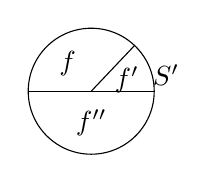
\begin{tikzpicture}\draw (0,0) circle (0.8); \draw (-0.8,0)--(0.8,0); \draw (0,0)--(0.55,0.58); \node at (-0.3,0.35) {$f$}; \node at (0.45,0.15) {$f'$}; \node at (0,-0.4) {$f''$}; \node at (0.95,0.2) {$S'$};\end{tikzpicture}\end{diagramblock} $f \cap f'' = S_0$}
ness" condition is now expressed by demanding that the set of indices
I can be totally ordered, \inserted[typed]{i.e. numbered} in such a way that we get X by succesively
"attaching" \unsure{Dells|cells} $D_{n(i)}$ to the space already constructed\xout{\unsure{,}} X(i-1), by a
map from \deleted{a}\inserted{a sub-} cell \xout{$D_i$}\inserted{of $D_{n(i)}$}, $S_j^{\hand{\varepsilon}} \to X(i-1)$ \quad $(\hand{\varepsilon\in\{}\pm 1\hand{\}})$ , this map of course
inducing an isomorphism,  more precisely \uline{the} standard isomorphism,\inserted{$\varphi^{\unsure{\varepsilon'}}_{n(i)}$}\deleted{of}
\margin{$\varphi^{\varepsilon'}_{n(i),j}$}
$S_j^{\hand{\varepsilon}} \simeq D_j$ \quad with\inserted{$S^{\varepsilon'}_j$} one of the two corresponding cells $S_j^+$ , $S_j^-$ in some
\margin{$S^{\varepsilon'}_j$}
$X_{i'} \simeq D_{n(i')}$ .  The \xout{xxxxx} dual translation of this\hand{,}in terms of fiber
products in \xout{xxx} a category C endowed with objects $F_i$ $(i\in\underline{N})$ and maps
$s_1^i , t_1^i$ between these, is clear:  for a given set of indices I and map
\margin{$P=\prod_{i\in I}F_{n(i)}$}
$i \mapsto n(i) : I \to \underline{N}$ , we consider a sub\xout{xxx}\inserted{-object of} $\inserted{P=}\hand{\prod_{i\in I}}F_{n(i)}$ ,  which can be
described by equality relations between it\over{t}{e}rated sources and targets
\xout{xxxxxx} of various components of $u = (u_i)_{i\in I}$  in P,  the structure of
the set of relations being such that I can\hand{\unsure{,}}be numbered, from 1 to N say,
in such a way that we get in succession \deleted{N}\inserted{$N-1$} relations on the N components
$u_i$ respectively,\inserted{$(2\leq i \leq N)$} every relation being of the type $f(u_i) = g(u_{i'})$ , with
f and g being iterated source or target maps, and $i'<i$ . \hand{(Whether}
\hand{source or target depending in obvious way on the two signs $\varepsilon,\varepsilon'$)}

\mspage{27}

\clearpage
% Pursuing Stacks (cotes 134-2 to 134-8): archive cote 134-2, site page 28 (PDF page 29).
% letter to Quillen. Draft compared: ps1.tex:660-736.
% AI-transcribed by Claude Opus 5.5 (claude-opus-5-5, adaptive thinking, effort high), Message Batches API, batch ps1 (msgbatch_01Rv5hCaNTtUt4JHx1yqoHPL), 2026-11-12; not yet checked by eye.
\scanpage{134-2/28}
\margin{8}
\mspage{\deleted{8} \hand{14}}
21.2.

\over{\unsure{4}}{8}. Returning to the\unsure{amalgamated|amalgamated} sum $X = \hand{\bigcup_i}X_i$ , the cellular decompositions
of the components $X_i \simeq D_{n(i)}$ define a cellular decomposition of X, whose
set of cells with incidence relation forms a finite ordered set K, fini-%
te union of a family of subsets $(K_i)_{i\in I}$ , with given isomorphisms\xout{m}
\[ f_i : K_i \simeq \underline{J}_{n(i)} \quad (i\in I) , \]
where for every index $n\in \underline{N}$, $\underline{J}_n$ denotes the ordered set of the 2n+1
cells $S_j^{\hand{\varepsilon}}$ $(0\leq j\leq n-1,\ \hand{\varepsilon\in\{}\pm 1\hand{\}})$, $D_n$ of the \deleted{pertinent} \inserted{relevant} cellular decomposition
of $D_n$ . We may without loss of generality assume there is no\deleted{t} inclusion
relation between the $K_i$ , moreover the standar\unsure{\over{t}{d}}ness condition described
above readily translates into a condition on this structure
$K$, $(K_i)_{i\in I}$ , $(f_i)_{i\in I}$ , and implies that for $i,i'\in I$, $K_i\hand{\cap}K_{i'}$ is a``clo-%
sed'' subset in the two ordered sets $K_i,K_{i'}$ (namely contains with any
element x the elements smaller than x), and moreover isomorphic (for the
induced order) to some $\underline{J}_n$ . Thus the category $B_o$ \xout{is} can be viewed as the
category of such ``standar\unsure{\over{t}{d}} ordered sets'' (with the extra structure on the-%
se just said), and the category $C_o$ can be defined most simply as the
dual category $B_o^{\,o}$ . (NB the definition of morphisms in $B_o$ is clear I
guess ...) I believe the category $B_o$ is stable under amalgamated sums
$X\amalg_Z Y$ , provided \inserted{however} we insist that the empty structure K is \uline{not} allowed -
otherwise we have to \xout{\unsure{insist}} restrict to amalgamated sums with $Z \neq \emptyset$ .
It seems finally more convenient to exclude the empty structure in $B_o$ ,
\margin{\unsure{(13!)}}
i.e. to exclude final element from $\underline{C}_o$ , for the benefit of being able to
\margin{* This is \unsure{obviously} false, see P.S. p.12}
state that $\underline{C}_o$ (and \uline{all categories $\underline{C}_n$}\hand{*} \deleted{\illegible{1}} \xout{\illegible{1}} \margin{(13!)} are stable under binary
amalgamated sums, and that the functors $\underline{C}_n\to C$ (and ultimately $\underline{C}_\infty\to C$)
we are interested in are just those commuting to arbitrary binary amalga-%
mated sums (without \xout{\illegible{1}} awkward reference to the objects $\underline{F}_i$ and the
iterated source and target maps between them ...)\hand{(13!)}.

\over{\illegible{1}}{9}. The category $\underline{C}_o$ being fairly well understood, \inserted{it} remains to complete
the construction by the inductive step, \inserted{\unsure{for)}} passing from $\underline{C}_n$ to $\underline{C}_{n+1}$ . The
main properties I have in mind \deleted{therefore} \inserted{for this}, for the sequence of categories
$\underline{C}_n$ and their limit $\underline{C}_\infty$ , are the following two.

A) For any $K\in Ob(\underline{C}_\infty)$ \ ($= Ob(\underline{C}_o)$), and any two arrows in $\underline{C}_\infty$
\[ f,g : K \rightrightarrows F_i , \]
with $i\in\underline{N}$, \hand{(}and such that either i=0, or the equalities
\[ \hand{(1)}\qquad s_1^i f = s_1^i g \ , \quad t_1^i f = t_1^i g \]
hold (case $i \over{>}{\geq} 1$), there exists $h: K\to F_{i+1}$ such that
\[ \hand{(2)}\qquad s_1^{i+1} h = f \ , \quad t_1^{i+1} h = g \ . \]
B) For any $n\in\underline{N}$, the category $\underline{C}_{n+1}$ is deduced from $\underline{C}_n$ by keeping
the same objects, and just adding new arrows \xout{\illegible{1}} h as in A), with
f, g arrows in $\underline{C}_n$ .

\margin{28}

\clearpage
% Pursuing Stacks (cotes 134-2 to 134-8): archive cote 134-2, site page 29 (PDF page 30).
% letter to Quillen. Draft compared: ps1.tex:723-786.
% AI-transcribed by Claude Opus 5.5 (claude-opus-5-5, adaptive thinking, effort high), Message Batches API, batch ps1 (msgbatch_01Rv5hCaNTtUt4JHx1yqoHPL), 2026-11-12; not yet checked by eye.
\scanpage{134-2/29}
\mspage{\unsure{\#5|8'}}

The expression ``deduce\unsure{s|d} from'' in B)  means that we are adding arrows
$h: K \to F_i$ (each with preassigned source and target in $\underline{C}_n$),  with as
``new axioms'' on \inserted{the bunch of} these uniquely the two relations \deleted{\illegible{1}}\inserted{(1),(2)} of \over{\illegible{1}}{A}), the category
$\underline{C}_{n+1}$  being deduced from $\underline{C}_n$ in an obvious way,  as the solution of a uni-%
versal problem with\inserted{in} the category of all categories where binary amalgama-%
ted products exist,  and ``maps'' between these being functors which commute
\margin{this has to be corrected -- amalgamated sums exist in \unsure{$C_\infty$} only, and these sho\unsure{uld} be respected}
to those fibered products\inserted{(14)}. \deleted{In}\inserted{In} practical terms,  the arrows of $\underline{C}_{n+1}$ are
those deduced from the arrows in $\underline{C}_n$ and the ``new'' arrows $h$,  by combining
formal operations of composing arrows by $v\circ u$ ,  and taking \inserted{(binary)} amalgamated
products of arrows. \deleted{\illegible{1}}

NB  Of course the condition (1) in A) is necessary for the existence
\margin{$\|$}of an $h$ satisfying (2).  That it is sufficient too \deleted{can}\inserted{may} be viewed as an
extremely strong,\xout{xxxxxxx} ``universal'' version of coherence conditions,
concerning the various structures introduced on a $\infty$-groupoid. Intuitive-%
ly,  it means that whenever we have \deleted{\over{\illegible{1}}{two} ways of}\inserted{two ways of} associat\unsure{i}ng to a \inserted{finite} family \deleted{\illegible{1}}
$(u_i)_{i\in I}$  of objects of an $\infty$-groupoid,  $u_i \in F_{n(i)}$ ,  \xout{xxxxxxxxxx} subjected
to a \hand{``}standar\over{t}{d}\hand{''} set of relations on the $u_i$'s, an element of some $F_n$ ,  in
terms of the $\infty$-groupoid structure only,  then we have automatically
\inserted[typed]{a ``homotopy''}\xout{xxxxxxxxxxx} between these built-in in the very structure of the $\infty$-%
groupoid,  provided it makes at all a sense to ask for one (namely provi-%
ded condition (1) holds if $n \geq 1$).   I have the feeling moreover that
conditions (A) and (B) (plus the relation $\underline{C}_\infty = \varinjlim \underline{C}_n$ ) is all what will
be ever needed,  when using the definition of the structure species,
- plus of course the description of $\underline{C}_o$ , and the \inserted{implicit} \unsure{fact} that the categories
\margin{inaccurate -- see above}
$\underline{C}_n$ are stable under binary fiber products and the inclusion functors com-%
mute to these\inserted{(13)}. Of course,  the category which really interests us is
$\underline{C}_\infty$,  the description of the intermediate $\underline{C}_n$'s\hand{$|$} is merely tec\over{\illegible{1}}{h}nical \deleted{txt} -
the main point is that there should exist an increasing sequence $(C_n)$ of
subcategories of $\underline{C}_\infty$ ,  having same objects\over{,}{(}and ``same'' fiberproducts\over{,}{)}\inserted{(13)},
such that $\underline{C}_\infty$ should be the limit (i.e. every arrow in $C_\infty$ should belong \deleted{\illegible{1}}
to some $\underline{C}_n$),  and such that the passage from $\underline{C}_n$ to $\underline{C}_{n+1}$ should satisfy \inserted{(B).}
\deleted{(B).} \hand{$\ulcorner$}It is fairly obvious that these conditions alone do by no means
caracterise $\underline{C}_\infty$  up to equivalence,  and still less the sequence of its
subcategories $\underline{C}_n$ .  The point I wish to make though,  before pursuing
with a proposal of an explicit description,  is \inserted{(firstly)} that \uline{this ambiguity is}
\uline{in the nature of things}\over{,}{.} \over{r}{R}oughly saying, two different mathematicians,
working independently on the conceptual problem I had in mind,  \deleted{\unsure{assuming}}\inserted{assuming}
they both wind up with some explicit definition,  will almost certainly
get non e\over{\illegible{1}}{q}uivalent definitions  -  namely with non equivalent categories
of (set-valued, say) $\infty$-groupoids !  And, secondly and as importantly,

\mspage{29}

\clearpage
% Pursuing Stacks (cotes 134-2 to 134-8): archive cote 134-2, site page 30 (PDF page 31).
% letter to Quillen. Draft compared: ps1.tex:771-835.
% AI-transcribed by Claude Opus 5.5 (claude-opus-5-5, adaptive thinking, effort high), Message Batches API, batch ps1 (msgbatch_01Rv5hCaNTtUt4JHx1yqoHPL), 2026-11-12; not yet checked by eye.
\scanpage{134-2/30}
\mspage{9}
\margin{\S 16}
that \uline{this ambiguity however is an irrelevant one.} To make this point
a little clearer, I could say that a third mathematician, informed of
the work of both, will readily think out a functor or rather a pair of
functors, associati\xout{m}ng to any structure of Mr. X one of Mr. Y and conver%
\hand{-}sely, in such a way that by composition of the two, we will associate
to a X-structure \hand{(}T say\hand{)} another T', which \deleted{of course} will not be isomor-%
phic to T of course, but endowed with a canonical \xout{xxxx} $\infty$-equivalence
(in the sense of Mr. X) $T \underset{\hand{\infty}}{\simeq} T'$ , and the same on the Mr. Y side. Most
probably, a fourth mathematician, faced with the same situation as the
third, will get \inserted{his own} \xout{\illegible{1}} pair of functors to reconciliate Mr X and Mr
Y , \inserted{which} \xout{\illegible{1}} very probably \xout{\unsure{his pair of functors}} won\hand{\unsure{'}}t be equivalent \xout{\illegible{1}} \hand{(}I mean
isomorphic\hand{)} to the previous one. Here however a fifth mathematician,
informed about this new perplexity, will probably show that the two
Y-structures U and U', associated by his two colleagues to \xout{the} an
X-structure T, while not isomorphic alas, admit however a canonical
$\infty$-equivalence between U and U'\inserted[typed]{(in the sense of the Y-theory)}. I could go on with a sixth mathematicia%
an, confronted with the same perplexity as the previous one, who winds
up with another \inserted{$\infty$-}equivalence between U and U' (without being informed of
the work of the fifth), and a seventh reconciling them by discovering
an $\infty$-equivalence between these equivalences. The story of course is
infinite, I better stop with seven mathematicians, a fair number now-%
adays to allow themselves getting involved with foundational matters ...
There should be a mathematical statement though resuming in finite terms
this infinite story, but in order to write it down I guess a minimum
amount of conceptual work, in the context of a given notion of $\infty$-grou-%
poids satisfying the desiderata (A) and (B) should be done, and I am by
no means sure I will go through this, not in this letter anyhow.

\margin{\unsure{ta.}} \hand{10.} Now in the long last the explicit description I promised of $\underline{C}_{n+1}$ \deleted{in} \inserted{in}
terms of $\underline{C}_n$ . As a matter of fact, I have a handful to propose ! One \margin{\unsure{n}}
choice, about the widest I would think of, is: for every pair (f,g)
in $\underline{C}_n$ satisfying condition (1) of (A), add one \xout{xxxxx} new arrow h. To
avoid set-theoretic difficulties though, we better \xout{xxxxxx} first modify
the definition of $\underline{C}_o$ so that the set of its objects should be in the
universe we are working in, preferably even it be countable. Or else
and more reasonably, we will pick one h for every isomorphism class of
situations (f,g) in $\underline{C}_n$ . Another restriction\hand{,} to avoid too much redundan-%
cy - this was the first definition actually that flipped to my mind the
day before yesterday - is to add a \uline{new} h only when there is no ``old''
one, namely in $\underline{C}_n$ , serving the same purpose. Then it came to my mind
that there is a lot of redundancy still\hand{;} \inserted[typed]{thus there would be already \deleted{in}}
\margin{30}

\clearpage
% Pursuing Stacks (cotes 134-2 to 134-8): archive cote 134-2, site page 31 (PDF page 32).
% letter to Quillen. Draft compared: ps1.tex:823-894.
% AI-transcribed by Claude Opus 5.5 (claude-opus-5-5, adaptive thinking, effort high), Message Batches API, batch ps1 (msgbatch_01Rv5hCaNTtUt4JHx1yqoHPL), 2026-11-12; not yet checked by eye.
\scanpage{134-2/31}
\mspage{9'}
infinitely many ope\xout{x}rations standing for the single ope\xout{\unsure{rat}}ion $v\overset{i}{\circ}u$ say,
which could be \unsure{wiewed|viewed} in effect in terms of an arbitrary n-sequence
($n\geqslant 2$) of "composable" i-objects $U_1=u,u_2=v,\ u_3.\dots\ u_n$ ;\inserted{just ``forgetting'' $u_3,\dots,u_n$!} The natural
way to meet this "objection" would be to restrict to \xout{a} pairs (f,g)
which cannot be factored non trivially through another object $K'$ as
\begin{diagramblock}\begin{tikzcd} K \ar[r] & K' \ar[r, shift left, "{f',g'}"] \ar[r, shift right] & F_i \end{tikzcd} .\end{diagramblock}
But even with such restrictions, there remain a lot of redundancies
- and this again seems to me in the nature of things, namely that there
is no really natural, "most economic" way for achieving condition (A),
by a stepwise construction meeting condition (B). For instance, in $\underline{C}_1$
already we will have \xout{the} not merely the compositions $v\overset{i}{\circ}u$ , but at the
same time simultaneous compositions
\[ (*) \qquad u_n\circ u_{n-1}\circ - - \circ u_1 \]
for "composable" sequences of i-objects ($i\geqslant 1$), without reducing this
(as is customary) to iteration of the binary composition $v\circ u$ . Of course
using the binary composition, and more generally iteration of $n'$-ary
compositions with $n'<n$ (when $n\geqslant 3$), we get an impressive bunch of
ope\xout{x}rations in the n variables $u_1$ , ..., $u_n$ , serving the same purpose
as (*). All these will be tied up by homotopies in the next step $\underline{C}_2$ .
We would like to think of this set of homotopies in $\underline{C}_2$ as a kind of
"transitive system of isomorphisms" (of associativity); now the transiti%
% NOTE: the right edge of the scan cuts the end of this line and of some following lines
vity relations one is looking for will be replaced by homotopies again
between compositions of homotopies, which will enter in the picture with
$\underline{C}_3$ ,\inserted{etc.} Here the infinite story is exemplified by the more familiar situa-%
\margin{$\otimes$} tion of the two ways in which one could define a\hand{"}\hand{$\otimes$}-composition with
associativity" in a category, \xout{\illegible{1}} starting \uline{either} in terms of
a binary operation, \uline{or}\inserted{with} a bunch of n-ary operations - with\hand{,} in both \deleted{cas\unsure{e}}\inserted{cases,}
the associativity isomorphisms being an essential part of the structure.
Here again, while it is generally (and quite validly) felt that the
two points of view are\hand{"}equivalent\hand{"}, and both have their advantages and
their drawbacks, still it is not true\inserted{I Believe} that the \inserted{two} categories of algebraic
\margin{$\otimes$} structures "category with associative \hand{$\otimes$}-operation", using one or the
\margin{* even not in the \unsure{grou-poid} context} other definition, are equivalent\hand{*}.\inserted{(15)} Here the story though of the relation
between the two notions is a \uline{finite} one, due to the fact that it is
related to the notion of 2-categories or 2-groupoids, instead of $\infty$ -
groupoids as before ...

Thus I do\hand{'}nt feel really like spending much energy in cutting down
redundancies, but prefer working with a notion of $\infty$-groupoid which \deleted{remain\unsure{s}}\inserted{remains}
partly indeterminate, the main features being embodied in the condition\unsure{\hand{s}}
(A) and (B) and in the description of $\underline{C}_0$ , without other specification.

\margin{31}

\clearpage
% Pursuing Stacks (cotes 134-2 to 134-8): archive cote 134-2, site page 32 (PDF page 33).
% letter to Quillen. Draft compared: ps1.tex:878-952.
% AI-transcribed by Claude Opus 5.5 (claude-opus-5-5, adaptive thinking, effort high), Message Batches API, batch ps1 (msgbatch_01Rv5hCaNTtUt4JHx1yqoHPL), 2026-11-12; not yet checked by eye.
\scanpage{134-2/32}
\mspage{10}

\margin{18}

\xout{\unsure{11}}11. One convenient way for constructing \xout{a} a category $\underline{C}_\infty$ would be to \deleted{defin}\inserted{define}
for every $K,L \in \mathrm{Ob}(\underline{C}_o) = \mathrm{Ob}(\underline{B}_o)$ the set $\mathrm{Hom}_\infty(K,L)$ as a subset of
the set $\mathrm{Hom}(|L|,|K|)$ of continuous maps \xout{xxxxx} between the geometric rea-%
lisations of L and K in terms of gluing together cells $D_i$ , the composi-%
tion of arrows in $\underline{C}_\infty$ being just composition of maps. This \unsure{amounts} to
defining $\underline{C}_\infty$ as \xout{a subcategory of} the dual of a category $\underline{B}_\infty$ of topologica\hand{l}
description\xout{s}. It will be sufficient to define for every cell $D_n$ and
every K a subset $\mathrm{Hom}_\infty(D_n,|K|)$\inserted{of $\mathrm{Hom}(D_n,|K|)$}, satisfying the two conditions:
a) stability \xout{with}\inserted{by} compositions $D_n \to |K| \to |K'|$, where $K \to K'$
is \xout{a}\inserted{an ``allowable''} continuous map, \inserted{namely} subjected only to the condition that its restriction
to any standar\over{t}{d} subcell $D_{n'} \subset |K|$ is again ``allowable'' i.e. in $\mathrm{Hom}_\infty$ .
b) Any ``allowable'' map $S_n^{\unsure{*}} \to |K|$ (i.e. whose restrictions to $S_n^+$ and
$S_n^-$ are allowable) extends to an allowable map $D_{n+1} \to |K|$.

Condition a) merely ensures stability of allowable maps under compo-%
sition, and the fact that $\underline{B}_\infty$ (endowed with the allowable maps as morphi\hand{s}-%
-ms) has the correct binary amalgamated sums, whereas b) expresses condi-%
tion \unsure{A|a}) on $\underline{C}_\infty$ . These conditions are satisfied when we take as $\mathrm{Hom}_\infty$
subsets defined by tameness conditions (such as piecewise linear for
suitable piecewise linear structure\inserted{on the $D_i$'s}, or differentiable etc). The condi-%
tion (B) however is of a subtler nature in \unsure{this|the} topological \xout{a}interpretation\hand{,}
and surely not met by such sweeping tameness requirements only ! Finally
the question as to whether we can actually in this way describe an ``accep-%
table'' category $\underline{C}_\infty$ , by defining sets $\mathrm{Hom}_\infty$ namely describing $\underline{C}_\infty$ in terms
of $\underline{B}_\infty$ , seems rather subsidiary\inserted{after all}. We may think of course of constructing
stepwise $\underline{B}_\infty$ via subcategories $\underline{B}_n$ , by adding stepwise new arrows in or-%
der to meet condition b), thus paraphrasing condition (B) for passage \xout{of}
from $\underline{C}_n$ to $\underline{C}_{n+1}$ - but it is by no means clear that when passing to the
\xout{sub}category $\underline{B}_{n+1}$ by composing \xout{arrows} maps of $\underline{B}_n$ and ``new'' ones, and
using amalgamated sums too, there might not be some \inserted{undesirable} extra relations
\xout{arising} in $\underline{B}_{n+1}$ , coming from the topological interpretation of the arrows
in $\underline{C}_{n+1}$ as maps. To say it differently, universal algebra furnishes us
readily with an acceptable sequence of categories $\underline{C}_n$ and hence $\underline{C}_\infty$ , and
by the universal properties of the $\underline{C}_n$ in terms of $\underline{C}_{n-1}$ , we readily get
(using arbitrary choices) a contravariant functor $K \mapsto |K|$ from $\underline{C}_\infty$ to
the category of topological spaces (i.e. a co-$\infty$-groupoid in (Top)), but
it is by no means clear that this functor is \uline{faithful} - and it does'nt
really matter after all !

\margin{32}

\clearpage
% Pursuing Stacks (cotes 134-2 to 134-8): archive cote 134-2, site page 33 (PDF page 34).
% letter to Quillen. Draft compared: ps1.tex:937-976 ; ps1.tex:976-1009.
% AI-transcribed by Claude Opus 5.5 (claude-opus-5-5, adaptive thinking, effort high), Message Batches API, batch ps1 (msgbatch_01Rv5hCaNTtUt4JHx1yqoHPL), 2026-11-12; not yet checked by eye.
\scanpage{134-2/33}
\mspage{\unsure{10.}}

\margin{\unsure{18|19}}

\deleted{\unsure{11}}\hand{12}. I think I really better stop now, except for one last comment. The
construction of a co-$\infty$-groupoid \inserted{$D_*$} in (Top), giving rise to the fundamental
functor
\[ \text{(Top)} \longrightarrow (\infty\text{-groupoids}), \qquad \hand{$X \longmapsto (\mathrm{Hom}(D_{\unsure{*|i}},X))_i$ ,} \]
generalises,as I already alluded to earlier, to the case when (Top) is
replaced by an arbitrary"model category"\inserted{$M$} in \deleted{your} \inserted{Quillen's} sense. Here however the
choices occur not only \inserted{stepwise} for the primary, secondary, ternary etc structures\hand{,}
but already for the primitive structure\hand{,} namely \inserted{by} choice of objects $D_i$ (\hand{$i\in\underline{N}$}
in M , and source and target maps $D_{\unsure{i}} \rightrightarrows D_{\unsure{i+1}}$ . These choices can be made
inductively, by choosing first for $D_o$ the final object, or more general-%
ly any object which is fibrant and trivial (over the final object), $D_{-1}$
being the initial object, and defining further $S_o$ \over{a}{=} $D_o\amalg_{D_{-1}} D_o = D_o \hand{$\amalg$} D_o$
with obvious maps \over{$\phi_o^+$}{$\psi_o^+$} , \over{$\phi_o^-$}{$\psi_o^-$} : $D_o \to S_o$ , and then \hand{,}if everything is constru\hand{-}
ted up to $D_n$ \deleted{\unsure{,}} and $S_n = (D_n,\phi_{n-1}^+)\amalg_{D_{n-1}}(D_n,\phi_{n-1}^-)$\hand{,} defining $D_{n+1}$ \deleted{\illegible{1}}\inserted{as} any
\margin{$D_{n+1}$}fibrant and trivial\inserted{(16)} object together with a cofibrant map
\[ S_n \longrightarrow D_{n+1} , \]
and $\phi_n^+ , \phi_n^-$ as the compositions of the latter with \hand{$\psi_n^+,\psi_n^-$} : $D_n \rightrightarrows S_n$ .
Using this and amalgamated sums in M, we get our functor
\[ \hand{$\underline{B}_o =$}\, \underline{C}_o^{\,o} \longrightarrow M \quad , \quad K \longmapsto |K|_M , \]
commuting with amalgamated sums, which we can extend stepwise through
the $\underline{C}_n^{\,o}$'s to a functor \inserted{$\underline{B}_\infty =$} $\underline{C}_\infty^{\,o} \to M$ , provided we know that the objects
$|K|_M$ of M ( $K \in \mathrm{Ob}\,\underline{C}_o$ ) obtained \xout{through} by "standar\over{t}{d}" gluing of the
$D_n$'s in M , are again fibrant and trivial - and I hope indeed that
your axioms imply that; via,say, that if $Z\to X$ and $Z \to Y$ are cofi\hand{b}rant
and X,Y,Z are fibrant and trivial, then $X\amalg_Z Y$ is fibrant and trivial \inserted{(17)}..

\margin{X}Among the things to be checked is of course that when we locali\over{s}{z}e
the category of \deleted{(}$\infty$-groupoids with respect to morphisms which are "weak
equivalences" in a rather obvious sense (NB the definition of the \hand{$\pi$}$_i$'s
of an $\infty$ -groupoid is practically trivial !) , we get a category equiva-%
lent to the usual homotopy category (Ho). Thus we get a composed functor
\[ M \longrightarrow (\infty\text{-groupoids}) \longrightarrow \text{(Ho)} , \]
as announced. I have some intuitive feeling of what this functor stands
for, at least when M is say the category of semisimplicial sheaves, or
(more or less equivalently) of n-\xout{groupoids}\inserted[typed]{gerbs} or $\infty$-\xout{groupoids}\inserted[typed]{gerbs}\inserted{(18)} on a given
topos: namely it \inserted[typed]{should} correspond\xout{s} to the operation of "integration" or"secti\hand{-}
ons" for n-gerbs (more generally for n-stacks) over a topos - which is
indeed \uline{the} basic operation (embodying non commutative cohomology objects
of the topos) in \hand{"}non commutative homological algebra\hand{"}.

I guess that's about it for today\hand{,} \over{i}{\unsure{I}}t's getting late and time to go
to bed ! Good night \hand{!}

\margin{33}

\clearpage
% Pursuing Stacks (cotes 134-2 to 134-8): archive cote 134-2, site page 34 (PDF page 35).
% letter to Quillen. Draft compared: ps1.tex:990-1057.
% AI-transcribed by Claude Opus 5.5 (claude-opus-5-5, adaptive thinking, effort high), Message Batches API, batch ps1 (msgbatch_01Rv5hCaNTtUt4JHx1yqoHPL), 2026-11-12; not yet checked by eye.
\scanpage{134-2/34}
\mspage{\hand{11}}

\mspage{10} 22.2.1983

\over{\unsure{12}}{13}. It seems I can't help pursuing further the reflection I started with
this letter ! First I would like to come back upon terminology. Maybe
to give the name of n-groupoids and $\infty$-groupoids to the objects I was af-%
ter is not proper, for two reasons: a) it conflicts with a standing
terminology, applying to structure species which are frequently met and
deserve names of their own, even if they turn out to be too restrictive
kind of objects for the use I am having in mind - so why not keep the ter-%
minology already in use, especially for two-groupoids, which is\xout{\unsure{thatxhad}}
pretty well suited after all; b) the structure species I have in mind
is not really a very well determined one, it depends as we saw on choices,
without any one choice looking convincingly better than the others - so
it would be a mess to give an unqualified name to such structure, depen-%
ding on the choice of a certain category $\underline{C}_{\infty} = \underline{C}$ . I have been thinking
of the terminology n-\uline{stack} and $\infty$-\uline{stack} (stack = ``champ'' in French),
a name introduced in Giraud's book (he was restricting to champs =
1-champs ), which over a topos reduced to a one-point space reduces in
his case to the usual notion of a category i.e. 1-category. Here of cour-%
se we are thinking of ``stacks of groupoids'' \unsure{rather|father} than arbitrary stacks,
which I would like to call (for arbitrary order n$\in\underline{N}$ or n=$\infty$) n-Gr-stacks
- suggesting evident ties with the notion of Gr-categories, we should
say Gr-1-categories, of Mme Hoang Xuan Sinh. One advantage of the \deleted{\unsure{namd}}\inserted{name}
``stack'' is that the use it had so far spantaneously suggests the extension
of these notions to the corresponding notions over an arbitrary topos,
which of course is what I am after ultimately. Of course, when an ambi-%
guity is possible, we should speak of \deleted{\illegible{1}} n-$\underline{C}$-stacks - the reference to
$\underline{C}$ should make superfluous the ``Gr'' specification. Thus n-$\underline{C}$-stacks are
essentially the same as n-\unsure{$\underline{C}$}-stacks over the final topos i.e. over a one
point space. When both $\underline{C}$ and ``Gr'' are understood in a given context, we
will use the \xout{\unsure{wordx"stack"}} terminology n-stack simply, or even``stack''
when n is fixed throughout. Thus it will occur that in certain contexts
``stack'' will just mean a usual groupoid, \xout{\unsure{in n=2 groupoid}} in others it
will mean just a category, \xout{\unsure{a n=2-category}} but when n=2 it will not mean
a usual 2-groupoid, but something more general, defined in terms of $\underline{C}$ .

The categories $\underline{C} = \underline{C}_{\infty}$ described before merit a name too - I would
like to call them ``\uline{coherators}'' (``\uline{coh\'ereurs}'' in French), \xout{\illegible{2}}
\over{t}{T}his name is meant to suggest that $\underline{C}$ embodies a hierarchy of coherence
relations, more accurately of coherence``homotopies''. When dealing with
stacks, the term \uline{i-homotopies} (rather than i-objects or i-arrows) for
the elements of the i$^{\mathrm{th}}$ component F$_{i}$ of a stack seems to me the most
suggestive - they will of course be denoted graphically by arrows,

\mspage{\hand{34}}

\clearpage
% Pursuing Stacks (cotes 134-2 to 134-8): archive cote 134-2, site page 35 (PDF page 36).
% letter to Quillen. Draft compared: ps1.tex:1047-1110.
% AI-transcribed by Claude Opus 5.5 (claude-opus-5-5, adaptive thinking, effort high), Message Batches API, batch ps1 (msgbatch_01Rv5hCaNTtUt4JHx1yqoHPL), 2026-11-12; not yet checked by eye.
\scanpage{134-2/35}
\mspage{27}

(such as hh: $f\to g$ in the formulation of (A) yesterday.) More specifical-%
ly, I will call coherator any category \uline{equivalent} to a category $\underline{C}_{\infty}$ \deleted{as} as
constructed before. \xout{\illegible{1}} Thus a coherator is stable under binary \deleted{amalga-}\inserted{fiber}
\deleted{mated sums}\inserted{products \deleted{\illegible{1}}}, moreover the $F_i$ are reco\xout{\unsure{m}}vered up to isomorphism as the inde-% \margin{(13!) false, see PS}
composable elements of $\underline{C}$ with respect to amalgamation.\hand{(13)} However, in a
category $\underline{C}_{\infty}$ , the objects $\underline{F}_i$ have non trivial automorphisms - namely
\margin{(14!), false, see below}\hand{(}the ``duality involutions'' and their compositions (the group of automor-%
phisms of $\underline{F}_i$ should turn out to be canonically isomorphic to $(\pm 1)^i$ \hand{(14)}) in
\xout{\unsure{and the $F_i$}} other words by the mere category structure of a coherator we
will not be able to recover the objects $\underline{F}_i$ in $\underline{C}$ up to unique isomorphism,
Therefore in the structure of a coherator should be included too the
choice of the basic undecomposable objects $\underline{F}_i$ (one in each isomorphism
class), and moreover the arrows $\underline{s}^i_1$ , $\underline{t}^i_1 : \underline{F}_i \rightrightarrows \underline{F}_{i-1}$ for $i\geq 1$ (a prio-%
ri, only the \uline{pair} $(\underline{s}^i_1 , \underline{t}^i_1)$ can be described intrinsically in terms
of the category structure of $\underline{C}$ , once $\underline{F}_i$ and $\underline{F}_{i+1}$ are chosen ...). But
it now occurs to me that we dont have to put in this extra structure after
all - while the $\underline{F}'_i$ s separately do have automorphisms, the system
of the objects $(\underline{F}_i)_{i\in\underline{N}}$ and of the maps $(\underline{s}^i_1)_{i\geq 1}$ and $(\underline{t}^i_1)_{i\geq 1}$ has only
the trivial automorphism (all this of course is heuristics, I did'nt
really prove anything - but the structure of the full subcategory of a
$\underline{C}_{\infty}$ formed by the objects $\underline{F}_i$ seems pretty obvious ... ). To finish get\xout{x}-%
ting convinced that the mere category structure of a coherator includes
already all other relevant structure, we should still describe a suitab-%
le intrinsic filtration by subcategories $\underline{C}_n$ . We define the $\underline{C}_n$ inductive%
ly, $\underline{C}_o$ being the``primiti\deleted{\unsure{y}}\inserted{ve} structure'' (the arrows are those deducible
from the source and target arrows by composition and \deleted{amalgamation}\inserted{fiber products}), and
$\underline{C}_{n+1}$ being defined in terms of $\underline{C}_n$ as follows: add to Fl $\underline{C}_n$ all arrows \margin{(25.2.) (20!) this may give however \uline{two} large a subcategory $\underline{C}_{n+1}$}
of $\underline{C}$ of the type $h\colon K\to \underline{F}_i$ $(i\geq 1)$ such that $\underline{s}^i_1 h$ and $t^i_1 h$ are in $\underline{C}_n$ , and
the arrows deduced from the bunch obtained \xout{through} by composition and
fibered products.\hand{(20)} In view of these constructions, it would be an easy
exercise to give an\inserted{intrinsic} caracterisation of a coherator, as a category satisfy
-ing certain internal properties.

I was a little rash right now when making assertions about the
structure of the group of auomorphisms of $\underline{F}_i$ - I forgot that two days
ago I pointed out to myself that even the basic operation inv$_i$ upon $\underline{F}_i$
need not \inserted{even} be \deleted{an} involution\hand{s}\inserted{(nor even automorphisms)}! However I just checked tha\xout{\unsure{q}}t if in the induc-% \margin{\deleted{nor even automorphisms}}
tive construction of coherators $\underline{C}_{\infty}$ given yesterday, we insist on the
most trivial irredundancy condition \hand{(} namely that we dont add a``new''
homotopy $h\colon f\to g$ when there is already an old one), then any morphism
$h\colon \underline{F}_i\to \underline{F}_i$ such that $\underline{s}\, f=\underline{s}$ and $\underline{t}\, f=\underline{t}$ , is the identity - and that

\margin{35}

\clearpage
% Pursuing Stacks (cotes 134-2 to 134-8): archive cote 134-2, site page 36 (PDF page 37).
% letter to Quillen. Draft compared: ps1.tex:1096-1169.
% AI-transcribed by Claude Opus 5.5 (claude-opus-5-5, adaptive thinking, effort high), Message Batches API, batch ps1 (msgbatch_01Rv5hCaNTtUt4JHx1yqoHPL), 2026-11-12; not yet checked by eye.
\scanpage{134-2/36}
\margin{12}
\mspage{12}

\inserted{implies} inductively that an automorphism of the system of $\underline{F}_i$'s  related by the
source and target maps $\underline{s}_1^i$ , $\underline{t}_1^i$  is the identity.  Thus it is correct afte\unsure{r}
% NOTE: the right edge of the scan cuts off the end of the line above
all, it seems,  that the category structure of a coherator implies all
other structure relevant to us\hand{(21)}.
\margin{\unsure{Maybe f th} it is safer to give moreover the $\underline{C}_o$ subcategory}

I do believe that the description given so far of what I mean by a
coherator, \xout{\illegible{1}} namely something acting like a kind of pattern in
order to define a corresponding notion of ``stacks'' (which in turn should
be the basic coefficient objects in non commutative homological algebra,
as well as a convenient description of homotopy types) embodies some of
the essential features of the theory \inserted[typed]{still in embryo} that wants to be developped. It is
quite possible of course that some features are lacking still ,  for in-%
stance that some extra conditions have to be imposed upon $\underline{C}$ ,  possibly
of a very different nature from mere irredundancy conditions (which, I
feel, are kind of irrelevant in this set-up).  Only by pushing ahead
and working out at least in outline the main aspects of the formalism of
stacks,  will it become clear whether or not extra conditions on $\underline{C}$ are
needed.  I would like at least to make a commented list of these main
aspects,  and possibly do some heuristic pondering on some of these in
the stride,  or afterwards.  For today it seems a little late though  -
I have been pretty busy with non mathematical work most part of the day,
and the next two days I'll be busy at the university.  Thus I guess I'll
send off this letter tomorrow,  and send you \unsure{a\xout{n}|an} \inserted{later} elaboration  (presumably
much in the style of this unending letter)  if you are interested.  In
any case I would appreciate any comments you make  -  that's why I have
been writing you after all !  I will probably send copies to Ronnie
Brown,  Luc Illusie and Jean Giraud,  in case they should be interested
(I guess at least Ronnie Brown is).  Maybe the theory is going to take
off after all,  in the long last !

Very cordially yours \hand{Alexander}

PS  (\unsure{23.2|25.2})  I noticed a rather silly mistake in the notes of two days
ago,when stating that the categories $\underline{C}_n$ admit fiber\xout{ed} products \unsure{\over{-}{:}} what is
\margin{\unsure{(1')}}
true is that the category $\underline{C}_o$ has fiber\xout{ed} products (by construction \inserted[typed]{practically}) \hand{\unsure{(1')}}
and that these are fiber\xout{ed} products also in the categories $\underline{C}_n$ (by con-%
struction equally) i.e. that the inclusion functors $\underline{C}_o \to \underline{C}_n$ commute to
fiber\xout{ed} products.  Stacks in a category C correspond to functors
$\underline{C}_\infty \to C$  whose \uline{restriction to $\underline{C}_o$} commutes with fiber products. I carried
the mistake along in the \xout{\illegible{1}} yesterday notes  -  it does'nt really
change anything substantially.  I will have to come back anyhow upon the
basic notion of a coherator ...

\margin{36}

\clearpage
% Pursuing Stacks (cotes 134-2 to 134-8): archive cote 134-2, site page 37 (PDF page 38).
% appendix (letters to Breen). Draft compared: ps1.tex:1144-1188.
% AI-transcribed by Claude Opus 5.5 (claude-opus-5-5, adaptive thinking, effort high), Message Batches API, batch ps1 (msgbatch_01Rv5hCaNTtUt4JHx1yqoHPL), 2026-11-12; not yet checked by eye.
\scanpage{134-2/37}
\mspage{23}

APPENDIX to Chapter I : three letters to Larry Breen

\xout{\unsure{1|I}} In this appendix, I am encluding three letters to Larry Breen, dated
5.2 , 17.2 and 17-19.7. 1975. These letters are written in French, and
the first two are reproduced textually, whereas the third appears here in
English translation. I am grateful to Ronnie Brown who took the trouble
last year to make such a translation\hand{(}from a hardly legible \xout{handwri} copy of
the handwritten letter to Larry Breen\hand{)} with the assistance of Larry Breen
himself and J.L. Loday. I am now using his translation rather than the
original letter, which no printer could possibly decipher !\hand{/}Also, for the
second letter I am using a typed copy made in 1975 by Larry Breen (who
presumably had difficulties too deciphering the handwriting)\unsure{,|.} Thanks are
due to him for his interest and patience (with someone like me, very un-%
knowledgeable in standard homotopy techniques), \deleted{\unsure{as it}}\inserted{which} appeared \deleted{from}\inserted{in} the
letters I got from him in response and his verbal explanations on related
matters,\inserted{as well as \deleted{from} in} the trouble he took in \xout{copying} retyping\inserted{that letter} and sending me copies of
my own letters to him, and allowing me to reproduce them in this volume
of P\over{u}{u}rsuing Stacks. My only present contribution to this set of letters is
adding a few comments (in the notes (\hand{22}) to (\hand{31})), \deleted{and correcting some}\inserted{adding subtitles (with numbers App. 1 to App. 18), and correcting some} \deleted{\illegible{1}}
inaccuracies in the English translation (due mainly to my handwriting ...)\hand{.}
Also, I skipped the beginning of the first letter, which does'nt seem \deleted{to}
\deleted{me} of general relevance.

The first two letters are an attempt to explain to Larry Breen (who
has a wide background in algebraic geometry and homological and homotopical
algebra) some of the main points of the programme I had in mind around the
notions of n-categories and n-stacks\unsure{\over{.}{,}} \hand{(}which is what I am supposed to be
pursuing now in my present work ``Pursuing Stacks''\hand{).}They were written under
the impetus of the\inserted{new} intuition \xout{which} (new to me at any rate) which then had
just appeared to me, namely that (non strict) n-groupoids should model
\margin{//}(in a suitable sense) n-truncated homotopy types.\hand{//} The third letter,\inserted{written in} ans-%
wer to a number of questions in Larry Breen's response to the first two,
is of a wider scope. A large part of the letter outlines (very ske\over{\unsure{t}}{tc}hyly)
some main points of a duality program (including a cohomological formula-%
tion of ``geometric'' local and global classfield theory), which \deleted{appears}\inserted{emerged by the end of the fifties and appears}
here for the first time in print\hand{,} \deleted{and going back to the end of the fif-%
ties.} \deleted{It}\inserted{The later part of the letter} gives also some hints about the need of a framework of ``tame to-%
pology'' suitable for writing up a ``dévissage theory'' of stratified spaces,
and for \xout{\illegible{1}}\inserted[typed]{working} with étale tubular neighbourhoods, for the common purpose
of coming to grips \deleted{of}\inserted{with} a suitable notion of ``fine\unsure{\hand{,}} homotopy type'' of a ``tame''
topological space or\inserted{of} a scheme\inserted{say}, in terms of the \deleted{ordered set}\inserted{inverse system} of ``indexed
homotopy types'' corresponding to\inserted{all} equisingular stratifications .

\margin{37}

\clearpage
% Pursuing Stacks (cotes 134-2 to 134-8): archive cote 134-2, site page 38 (PDF page 39).
% appendix (letters to Breen). Draft compared: ps1.tex:1174-1193.
% AI-transcribed by Claude Opus 5.5 (claude-opus-5-5, adaptive thinking, effort high), Message Batches API, batch ps1 (msgbatch_01Rv5hCaNTtUt4JHx1yqoHPL), 2026-11-12; not yet checked by eye.
\scanpage{134-2/38}
\mspage{\hand{23 bis}}
% NOTE: the typed text is on a slip pasted onto another typed page; text of the underlying page shows through faintly and is not transcribed

\hfill Villecun 5.2.1975

\margin{--} Cher Breen

\quad ....

(App.1) \quad ... Pour tout le reste de ta lettre, \ elle mériterait un lecteur
\margin{--} plus averti, \ aussi, \ pour qu'elle ne soit pas entièrement perdue au monde,
je vais l'envoyer à Illusie ! \ J'ai néanmoins
constaté\hand{,} avec intérêt\hand{,} ton intérêt à demi \unsure{rèfoulé|refoulé} pour des 2-catégories de
Picard, n-catégories et autre faune de ce genre, et ton espoir que je te
prouverai peut-être que ces animaux sont tout à fait indispensables pour
faire des maths sérieuses \ dans telle ou telle circonstance. J'ai bien \hand{peur}
que cet espoir ne soit déçu, je crois que jusqu'à maintenant on a toujours
pu s'en tirer en éludant de tels objets et l'engrenage dans lequel ils pour
-raient nous entrainer. Est-ce nécessairement une raison pour continuer à
les éluder ? Les situations où on a l'impression"d'éluder" en effet me sem-%
blent en tous cas devenir toujours plus nombreuses - \ et si on s'abstenait
de tirer une situation complexe et chargée de mystère au clair, chaque
fois qu'on ne serait pas \uline{forcé} de le faire pour des raisons techniques pro-%
venant de la math déjà faite, - il y aurait sans doute beaucoup de parties
des maths aujourd'hui reputées\hand{|}"sérieuses" qui n'auraient jamais \inserted{été} développées
(Il n'est pas dit non plus que\hand{|}le monde s'en trouverait plus mal ...). Ton
commentaire (que j'ai également entendu chez Deligne) \ que la classificati-%
on d'objets géométriques relativement merdiques se réduit finalement à des
invariants cohomologiques essentiellement "bien connus" et relativement
simples n'est pas non plus convainquant; n'est ce pas négliger la différen-%
ce entre la \uline{compréhension d'un objet géométrique}, et la détermination de
sa "classe à isomorphisme (ou équivalence...) près" ?

\margin{38}

\clearpage
% Pursuing Stacks (cotes 134-2 to 134-8): archive cote 134-2, site page 39 (PDF page 40).
% appendix (letters to Breen). Draft compared: ps1.tex:1193-1197.
% AI-transcribed by Claude Opus 5.5 (claude-opus-5-5, adaptive thinking, effort high), Message Batches API, batch ps1 (msgbatch_01Rv5hCaNTtUt4JHx1yqoHPL), 2026-11-12; not yet checked by eye.
\scanpage{134-2/39}
\mspage{24}

Tu me demandes des exemples "convainquants" de 2-catégories de Picard.
Voici quelques \deleted{uns}\inserted{exemples,} en vrac \hand{(je ne sais s'ils seront convainquants !)}:

\margin{$\times$(22)} 1) Si L est un lien\inserted{(22)} de centre Z sur le topos X, les \uline{gerbes liées par Z}
forment une 2-catégorie de Picard stricte, représentée par le complexe
$R\hand{\Gamma}_X(Z)$ tronqué en degré 2, dont les objets de cohomologie non triviaux
sont \unsure{Hes|les} $H^i(X,Z)$, $0 \hand{\leqslant} i \hand{\leqslant} 2$. Les \over{\unsure{g}}{g}erbes liées par L forment un \uline{pseudo-2-}
\uline{torseur} sous la gerbe précédente, qui est un 2-torseur\hand{(}i.e. non vide\hand{)} sss
une certaine obstruction dans $H^3(X,Z)$ est nulle. Pour comprendre \unsure{cette}
classe de notre point de vue, il y a lieu de passer aux 2-champs \unsure{corres-|derres-}%
pondants: le 2-champ de\xout{s} Picard \inserted[typed]{strict,} des Z-gerbes\xout{\unsure{liées par Z et le 2-champ des}}
sur des objets variables de X, et le 2-champ des L-gerbes sur des objets
variables. Ce dernier est bel et bien un 2-torseur sous le champ précédent,
or la classification de ces \xout{deux} 2-torseurs (à 2-équivalence près) se
fait par le $H^3(X,Z)$, \xout{de façon précise} \hand{(}tout comme les Z-\inserted{1-}gerbes peuvent être
interpétées comme des \xout{\unsure{1}}torseurs sous la Z-1-\over{\unsure{gerbe}}{champ} \inserted[typed]{de Picard strict,} des Z-torseurs, et sont
\xout{par conséquent} classifiées par le $H^2(X,Z)$\hand{)}. On voit déjà, bien sûr, poindre
ici l'oreille de la 3-catégorie de Picard stricte des 2-gerbes liées par Z,
ou (de façon équivalente) des 2-torseurs sous le 2-champ de \unsure{Picard} strict
des Z-1-gerbes; cette 3-catégorie de Picard stricte étant décrite par
$R\hand{\Gamma}_X(Z)$ tronqué en dimension 3, ayant comme invariants de cohomologie non
triviaux les $H^i(X,Z)$ $(0 \hand{\leqslant} i \hand{\leqslant} 3)$. Quant au 3-champ de Picard \unsure{correspondaht|correspondant},
il est décrit par une résolution injective de Z \hand{tronquée} en degré 3, alors
que le  2-champ de Picard précédent se décrivait en tronquant en degré 2.

2. Si M et N sont deux faisceaux abéliens sur X, les \uline{champs de Picard}
(NB: 1-champs !) \uline{d'invariants} M \uline{et} N forment eux-même une\inserted{2-}catégorie de
\margin{$\times$} Picard stricte, représentée  sans doute par le complexe RHom(X(M),N) \inserted{(23)}
tronqué en \xout{dimension} degré 2, dont les invariants de chomologie non trivi-%
aux sont donc \hand{``}le drôle de $\mathrm{Ext}^2$\hand{''} de ma lettre à Deligne, et les Honnètes
$\mathrm{Ext}^i(M,N)$  $(0 \hand{\leqslant} i \hand{\leqslant} 1)$. Les champs de Picard stricts forment une sous-2-caté%
gorie de Picard pleine, représentée par RHom(M,N) tronqué en degré 2,
d'invariants les $\mathrm{Ext}^i(M;N)$ $(0 \hand{\leqslant} i \hand{\leqslant} 2)$. Bien sûr, $\mathrm{Ext}^2$ donne les\inserted{0-}objets à
équivalence près, $\mathrm{Ext}^1$ les automorphismes à isomorphisme près de l'objet
nul, $\mathrm{Ext}^0$ les automorphismes de l'automorphisme identique audit ... Je n'ai
pas réfléchi à une bonne \unsure{interprétation} géométrique de la n-catégorie de
Picard associée à RHom(M,N) tronqué en degré n, et encore moins bien \xout{s}sûr
pour RHom(X(M),N), mais sans doute il faut regarder dans la direction des
n-champs de Picard.

3. Soit G un Groupe sur X, opérant sur un faisceau abélien N. Les \uline{champs}
\uline{en} (Gr)-\uline{catégories sur} X \uline{liés par} (G,N) forment une 2-catégorie de Picard,

\mspage{39}

\clearpage
% Pursuing Stacks (cotes 134-2 to 134-8): archive cote 134-2, site page 40 (PDF page 41).
% appendix (letters to Breen). Draft compared: ps1.tex:1195-1203.
% AI-transcribed by Claude Opus 5.5 (claude-opus-5-5, adaptive thinking, effort high), Message Batches API, batch ps1 (msgbatch_01Rv5hCaNTtUt4JHx1yqoHPL), 2026-11-12; not yet checked by eye.
\scanpage{134-2/40}
\mspage{\hand{25}}

dont les invariants sont $H^3(B_G \text{ mod } X,N)$, $H^2(B_G \text{ mod } X,N)$, et $Z^1(G,N)$ (groupe
des 1-cocyles de $G$ à coéfficients dans $N$)- je te laisse le soin de deviner
quel est le complexe tronqué qui le décrit ! J'ai écrit il y a quelques
mois à Deligne à ce sujet, et l'ai prié de t'envoyer une copie de \xout{\unsure{envoyer}}
la lettre.

4) Soit $X$ un topos localement annelé, on peut considérer les \uline{Algèbres
d'Azumaya sur} $X$ (i.e. les Algèbres localement isomorphes à une alg. de
matrices d'ordre $n$, $n \geq 1$) comme les objets d'une 2-catégorie de Picard,
où la catégorie $\underline{\mathrm{Hom}}(A,B)$, pour $A$ et $B$ des Algèbres d'Azumaya, est la caté-%
gorie des ``trivialisations'' de $A^o\otimes B$, i.e. des couples $(E,\emptyset)$, $E$ un Module
localement libre et $\emptyset$ un isomorphisme $\underline{\mathrm{End}}(E)\simeq A^o\otimes B$. Il faut travailler
un peu pour définir les accouplements\xout{x} $\underline{\mathrm{Hom}}(A,B)\mathrm{x}\underline{\mathrm{Hom}}(B,C)\hand{\to}\underline{\mathrm{Hom}}(A,C)$; l'opé-%
ration $\otimes$ dans la 2-catégorie de Picard à construire est bien sûr le produit
tensoriel d'Algèbres, et l'opération ``puissance $-1$'' est le passage à l'al-%
gèbre opposée. On \unsure{vérfie|vérifie}\xout{,xx passant aux champs correspondant, qui sont} qu'en
associant à toute Algèbre d'Azumaya la 1-gerbe de ses trivialisations, on
trouve un 2-$\otimes$-foncteur de la 2-catégorie de Picard (dite ``de Brauer'') dans
celle des 1-gerbes liées par $\underline{G}_m$ , qui est 2-fidèle. Les invariants de
la première sont donc les groupes $H^2(X,\underline{G}_m)_{Br}$ , $H^1(X,\underline{\unsure{H|G}}_m)$ et $H^o(X,\underline{G}_m)$ , où
dans le premier terme l'indice Br désigne le sous-groupe du $H^2$ formé des
classes de cohomologie provenant d'Algèbres d'Azumaya. On aurait envie
de parler du 2-champ de Picard des Algèbres d'Azumaya sur des objets variab
les de $X$, mais c'est bien une 2-catégorie de Picard fibrée sur $X$, mais pas
tout à fait un 2-champ (whatever that means), sans doute - la condition de
2-recollement (whatever that means) ne doit pas être satisfaite - sinon il
n'y aurait pas d'indice Br au $H^2$ ...
\margin{espace}

\inserted{(App.2)} La considération des $n$-catégories de Picard \inserted[typed]{strictes} (qui s'imposent à nous pas
à pas dans un contexte essentiellement ``commutatif'') me semblent la clef du
passage de l'algèbre homologique ordinaire (``commutative''), en termes de
complexes, à une algèbre homologique non commutative, du fait qu'elles
donnent une interprétation géométrique correcte des ``complexes tronqués à
l'ordre $n$'' \inserted{(en tant \unsure{qu'objets|qui objets} de catégories dérivées)}, donc, essentiellement (par passage à la limite sur $n$) des
complexes tout courts. L'idée naive qui se présente est alors que les
``complexes non commutatifs'' (qui seraient les objets-fantômes d'une algèbre
homologique non commutative) sont peut-être ce qui reste des $n$-catégories
de Picard (strictes) quand on oublie \unsure{leut|leur} caractère additif, i.e. leur
structure de Picard - c'est à dire qu'on ne retient que la $n$-catégorie !
\inserted{(Quand on se place sur un topos $X$, on s'intéresse donc aux $n$-champs sur $X$...)}
A vrai dire, cette idée est venue d'abord d'une autre direction, quand il
s'est agi en géométrie algébrique de démontrer des \uline{\deleted{formules}\inserted{théorèmes} de Lefschetz}

\margin{\hand{40}}

\clearpage
% Pursuing Stacks (cotes 134-2 to 134-8): archive cote 134-2, site page 41 (PDF page 42).
% appendix (letters to Breen). Draft compared: ps1.tex:1203-1205.
% AI-transcribed by Claude Opus 5.5 (claude-opus-5-5, adaptive thinking, effort high), Message Batches API, batch ps1 (msgbatch_01Rv5hCaNTtUt4JHx1yqoHPL), 2026-11-12; not yet checked by eye.
\scanpage{134-2/41}
\mspage{\hand{26}}

\inserted{en cohomologie étale}
à coéfficients discrets\hand{(}, dans le cas d'une variété projective disons et
de toute section hyperplane, ou d'une variété quasi-projective et de presque
toute section hyperplane (pour ne mentionner que le cas global le plus sim-%
ple), sous les hypothèses de profondeur\hand{(}\inserted[typed]{cohomologique} ``les plus naturelles'' (en fait,
essenti\over{\unsure{a}}{e}llement des conditions néc. et suff. de validité dudit théorème).
Dans le cas commutatif, les techniques de dualité nous suggèrent très clai-%
rement quels sont les meilleurs énoncés possibles, cf. l'exposé de Mme Ray-%
naus dans SGA 2. Mais ces techniques ne valent qu'en se restreignant à des
coéfficients premiers aux caractéristiques, alors que des démonstrations
directes plus géométriques (développées dans SGA 2 av\over{\unsure{e}}{a}nt le développement
du formalisme de la cohomologie étale) donnaient des résultats très voisins
\margin{$\pi_0,\pi_1$}pour le H$^0$ et le H$^1$ (ou le\inserted{$\pi_0$ et le} $\hand{\pi}_1$ , si on préfère) sans telles restrictions,
du moins dans le cas propre (i.e. projectif, au lieu de quasi-projectif).
En fai\hand{t}, ce sont \deleted{\unsure{aussi}} \over{\unsure{d}}{l}es ``résultats les meilleurs possibles'' eux-%
mêmes, énoncés comme conjectures dans SGA 2 dans l'exposé cité de Mme \over{\unsure{R}}{R}ay-%
naud, qui sont démontrés ultérieurement par elle dans sa thèse. Ce qui est
remarquable de notre point de vue, c'est que les énoncés les plus forts se
présentent le plus naturellement sous forme d'énoncés sur des\inserted{1-}\uline{champs} sur
le site étale de la variété algébrique considérée - la notion de ``profon-%
deur $\geq$ i'' (pour i=\over{\unsure{1}}{1},2,3) s'énonçant aussi le plus naturellement en termes
de champs. Non seulement cela, mais alors même qu'on voudrait ignorer la
notion technique de champ et travailler exclusivement en termes de H$^0$ et
H$^1$en utilisant à bloc le formalisme\inserted{cohomologique non commutatif} de Giraud, pour démontrer disons un
théorème de bijectivité $\hand{\pi}_1$(Y)$\hand{\to}\hand{\pi}_1$(X) (ce qui est le résultat le plus pro-%
fond établi dans la thèse de Mme Raynaud), il semble bien qu'on n'y arrive\hand{\unsure{''}}
\xout{xxxx} pas, faute \xout{dxxxxixxa} à ce formalisme d'avoir la souplesse nécessaire\hand{.}
En fait, il faut utiliser comme ingrédients techniques, de façon essentielle\hand{,}
les trois théorèmes suivants directement pour les 1-champs ``de torsion''
(i.e. où les faisceaux en groupes d'automorphismes sont de ind-torsion):
a) théorème de changement de base pour un morphisme propre, b) théorème de
changement de base par un morphisme lisse  c) théorème de \xout{xhanx} ``propreté
cohomologique générique'' pour un morphisme de type fini f: X$\to$S, S intègre
(disant que l'on peut trouver dans S un ouvert U$\neq\emptyset$ tel que pour \uline{tout} change
ment de base S'$\to$ S se factorisant par u, la formule de changement de base
est vraie). \hand{(}Pour b) et c), il faut faire des hypothèses que les fais\unsure{d}eaux
d'automorphismes sont premiers aux cara\unsure{ct}érisitques, et dans c) une hypothè
se de constructtibilité sur ces faisceaux - mais b) et c) ne servent que
dans la version ``générique'' du th. de Lefschetz.\hand{)} C'est avec en vue de telle\hand{s}
applications que Giraud a pris la peine dans son bouquin (si je ne me trompe\hand{)}
de demontrer a)\hand{,} b) (et c) ?) dans le contexte des 1-champs et de leurs

\margin{41}

\clearpage
% Pursuing Stacks (cotes 134-2 to 134-8): archive cote 134-2, site page 42 (PDF page 43).
% appendix (letters to Breen). Draft compared: ps1.tex:1203-1212.
% AI-transcribed by Claude Opus 5.5 (claude-opus-5-5, adaptive thinking, effort high), Message Batches API, batch ps1 (msgbatch_01Rv5hCaNTtUt4JHx1yqoHPL), 2026-11-12; not yet checked by eye.
\scanpage{134-2/42}
\mspage{27}

images directes et inverses. Mais du même coup il devient clair que le
contexte ``naturel'' des théorèmes de changement de base en cohomologie étale,
des théorèmes\inserted{du type} de Lefschetz (dits ``faibles'') sur les ``sections hyperplanes'',
tout comme \inserted{de} la notion de profondeur qui y joue un rôle crucial, \hand{doit} \inserted{être} celui
des n-champs. Et que le développement hypothétique de ce contexte\deleted{,} ne ris-%
que pas de se réduire à une jonglerie purement formelle et absolument bor-%
délique avec du ``general nonsense'', mais qu'on se trouvera aussitôt confron-%
té à des tests ``d'utilisabilité'' aussi sérieux que la démonstration des
théorèmes de changement de base et ceux du type de Lefschetz (qui même
dans le contexte commutatif ne sont pas piqués de vers ...). \hand{Idem pour
variantes analytiques complexes etc.}

Je ne sais si ces commentaires te ``passent par dessus la tête'' à ton
tour, ni si elles te donnent l'impression qu'il y aurait peut-être des cho-%
ses intéressantes à tirer au clair. Si cela t'intéresse, je pourrais expli-%
citer sous forme un peu plus systématique quelques ingrédients d'une hypo-%
thétique algèbre homologique non commutative et les liens de celle-ci à
l'algèbre homologique commutative. Plus mystérieux pour moi (et pour cause,
vu mon ignorance en homotopie) seraient les relations entre celle-là et
l'algèbre homotopique, I.e. les structures semi-simpliciales, et je n'ai
que des commentaires assez vagues à faire en ce sens\hand{(*)}.Par ailleurs, je te
rappelle que même l'algèbre homologique \xout{\illegible{1}} commutative n'est pas, il s'en
faut, dans un état satisfaisant, pour autant que je sache, vu qu'on ne sait
\margin{(24)} toujours pas quelle est la ``bonne'' notion de catégorie triangulée\hand{\unsure{(*)}}. Or il me
semble bien clair que ce n'est pas une question purement académique - même
si on a pu se passer de le savoir jusqu'ici (en se bornant comme Monsieur
Jourdain à ``faire de la \unsure{prosé|prose} sans le savoir'' - en travaillant sur des
catégories de complexes, éventuellement filtrés, sans trop se demander quel
-les structures il y a sur ces catégories ...).

Bien cordialement à toi

\hand{A Grothendieck}

\margin{(App.3)} \hand{(*) P.S.} Réflexion faite, j'ai quand même envie de te mettre un peu en ap-%
pétit, en faisant ces ``quelques commentaires assez vagues\hand{''}. Il s'agit du
yoga qu'une \inserted{\deleted{\illegible{1}} (petite)} n-catégorie \inserted{\unsure{en groupoïdes|ou groupoïdes}} (à n-équivalence près \deleted{\unsure{``est}} \inserted{``est} essentiellement la même
chose'' qu'un ensemble semi-simplicial pris à homotopie près et où on négli-%
ge les \hand{$\pi$}$_i$ pour i \hand{$\geq$} n+1 (où, si tu préfères,``où on a tué les groupes d'homo-%
topie en dimension \hand{$\geq$}n+1''). Voici des éléments heuristiques pour ce yoga.
Si K. est un ensemble simplicial (il peut être prudent de le prendre de
Kan) on lui associe une n-catégorie \xout{\unsure{Kx}} C$_n$(K.), dont les 0-objets sont les

\margin{42}

\clearpage
% Pursuing Stacks (cotes 134-2 to 134-8): archive cote 134-2, site page 43 (PDF page 44).
% appendix (letters to Breen). Draft compared: ps1.tex:1210-1212.
% AI-transcribed by Claude Opus 5.5 (claude-opus-5-5, adaptive thinking, effort high), Message Batches API, batch ps1 (msgbatch_01Rv5hCaNTtUt4JHx1yqoHPL), 2026-11-12; not yet checked by eye.
\scanpage{134-2/43}
\mspage{28}

O-simplexes, les 1-objets sont les chemins \xout{entre} (ou homotopies) entre
O-simplexes, les 2-objets sont les homotopies entre chemins (à extrémités fi-%
xées) etc. Pour les n-objets, cependant, on ne prend pas les homotopies
entre homotopies de fourbis, mais classes d'équivalence \xout{\unsure{entre}}\hand{\unsure{d'}}homotopies
(modulo la relation d'homotopie) entre homotopies. La composition des
i-objets ($i\hand{\geq}1$) se définit de façon évidente, on notera qu'elle n'est pas
strictement associative, mais associative modulo homotopie. Donc la n-caté-%
gorie qu'on obtient n'est pas"stricte" - et on prévoit pas mal d'emmerdement
pour définir de façon raisonnable une n-catégorie pas stricte (dans la
\unsure{déscription}\hand{/}des compatibilités \xout{entre} pour les "données d'associativité\hand{"}). La
mise sur pied du yoga qui suit pourrait constituer un fil d'\hand{A}riane pour la
définition en forme des n-c atégories (pas strictes), les n-foncteurs entre
elles (pas non plus stricts, et pour cause), les n-équivalences etc, au
même t\unsure{\xout{u}}itre que le yoga initial "une n-catégorie est une catégorie ou les
Hom et leurs accouplements\inserted{de composition} sont des(n-1)-catégories et des accouplements
entre telles". Cette n-catégorie\inserted{$C_n(K.)$} dépend fonctoriellement de $K.$ , tout
morphisme simplicial $K. \hand{$\to$} K'.$ définit un n-foncteur $C_n(K.)\hand{$\to$}C_n(K'.)$; en
fait, cela doit en dépendre même n-fonctoriellement, vu qu'on voit (en s'in%
spirant de ce qui précède et l'appliquant à des ensembles semi-simpliciaux
de la forme $Hom.(K.,K'.)$) que les ensembles semi-simpliciaux forment eux-%
mêmes \xout{une}\inserted{les O-objets d'une} n-catégorie, quel que soit $\unsure{N|n}$ ...

En fait, $C_n(K.)$ est un\xout{e} n-groupoïde, i.e. une n-catégorie où toute
i-fléche ($1\leq i\leq n$) (= i-objet) est une "équivalence" i.e. admet un quasi-%
inverse (donc un inverse si la n-catégorie est"réduite"). Si C est une
telle n-c atégorie i.e. un n-groupoïde, et x un O-objet de C, il s'impose
de désigner par $\hand{$\pi_i$}(C,x)$ ($O\leq i\leq n$) successivement: l'ensemble des classes
de O-objets à équivalence près (c'est un vulgaire ensemble), l'ensemble des
classes à équivalence près de 1-objets\hand{(}ou 1-flèches\hand{)} $x \to x$ (c'est un groupe,
pas nécessairement commutatif), l'ensemble des\inserted{classes mod équivalence des} 2-flèches $1_x \to 1_x$ , où $1_x$
est la 1-flèche identique de x (c'est un groupe commutatif $\hand{$\pi$}_2(C,x)$, ainsi
que les groupes qui vont suivre), l'ensemble des classes mod équivalence
de 3-flèches $1_{1_x} \longrightarrow 1_{1_x}$ , etc. Ces groupes forment, comme de juste, des
"systèmes loc aux" sur l'ensemble des O-objets de C, et modulo le grain de
sel habituel,\inserted{les $\pi_i(C,x)$} ne dépendent que de la"composante connexe" du O-objet x i.e.
de sa classe modulo équivalence de O-objets. Ceci dit, si C est de la form\unsure{e}
$C_n(K.)$, il résulte pratiquement des définitions que \xout{les} l'on a des isomor%
phismes canoniques $\hand{$\pi$}_i(K.,x)\hand{$\simeq$}\hand{$\pi$}_i(C_n(K.))$ pour $0\leq i\leq n$, qui pour x variable
peuvent s'interpréter comme des \over{\illegible{1}}{i}somorphismes de systèmes locaux. Il s'en-%
suit que pour une application semi-simpliciale \hand{$f$}:$K. \hand{$\to$} K.'$, le n-foncteur
correspondant $C_n(K.) \hand{$\to$} C_n(K.')$ est une n-équivalence sss f induit un iso-%

\margin{43}

\clearpage
% Pursuing Stacks (cotes 134-2 to 134-8): archive cote 134-2, site page 44 (PDF page 45).
% appendix (letters to Breen). Draft compared: ps1.tex:1212-1216.
% AI-transcribed by Claude Opus 5.5 (claude-opus-5-5, adaptive thinking, effort high), Message Batches API, batch pilot (msgbatch_0189Nhf1xB615YWnztubtLfc), 2026-11-12; not yet checked by eye.
\scanpage{134-2/44}
\mspage{29}

morphisme sur les $\hand{\pi}_0$ et sur les $\hand{\pi}_i$ en tout point (1\hand{$\leq$}i\hand{$\leq$}n). On serait plus
heureux de pouvoir dire à la place ``et \inserted{de plus} un homomorphisme surjectif pour
i=\over{N}{n}+1'', car c'est, il me semble, cela qu'il faudrait pour \inserted{espérer} pouvoir conclure
que la catégorie localisée de la catégorie des ensembles semi-simpliciaux,
obtenue en inversant les flèches\hand{\textbackslash}``qui induisent des isomorphismes sur les
$\hand{\pi}_i$ pour 0\hand{$\leq$}i\hand{$\leq$}n'' (ou encore,``en négligeant''les ensembles semi-simpliciaux
n-connexes), est équivalente à la catégorie localisée de la catégorie des
n- catégories, où on rend inversibles les n-équivalences ? Quoi qu'il en
soit, ces petites bavures devraient disparaitre lorsqu'on ``stabilise'' en
faisant augmenter n. A ce propos, on voit que le foncteur ``tron\over{\illegible{1}}{ca}ture en
dim. n'' de la théorie homotopique (consistant à tuer les groupes d'homotopi
% NOTE: the end of this line is cut off at the right edge of the scan ("homotopi...")
à partir de la dimension n\unsure{\hand{+1)}}.s'interprète dans le langage des n-catégories
par l'opération faisant passer d'une N-catégorie (N\hand{$>$}n) à une n-catégorie,
en conservant \xout{\illegible{2}} tels quels les i-objets (0\hand{$\leq$}i\hand{$\leq$}n-1) et leur
composition (1\hand{$\leq$}i\hand{$\leq$}n-1), et en remplaçant les n-objets par les classes \xout{d'}
\xout{\unsure{équivalence}} de n-objets ``à équivalence près'', avec la composition obtenue
par passage au quotient. De même, le foncteur d'inclusion évident en
théorie homotopique, consistant à regarder un ensemble semi-simplicial
``où on a négligé les $\hand{\pi}_i$ pour i\hand{$\geq$}n+1'' comme un ensemble semi-simplicial \xout{qui}
(dans la catégorie homotopique) qui se trouve avoir des $\hand{\pi}_i$ nuls pour
i\hand{$\geq$}n+1, se traduit par le foncteur allant des n-catégories vers les N-%
catégories, obtenue en ajoutant à une n-catégorie des i-flèches (n+1 \hand{$\leq$}i\hand{$\leq$}N)
identiques exclusivement. (Ainsi, un ensemble est regardé comme une catégo-%
rie ``discrète'', une catégorie comme une 2-catégorie où les \uline{Hom}(A,B), A et B
des 0-objets, sont des catégories discrètes, etc ...).

Bien entendu, rien n'empêche de considérer aussi la notion de $\hand{\infty}$-catégo-%
% NOTE: line end cut at the right edge; a hyphen after "catégo" may be hidden
rie, à laquelle celle de n-catégorie est comme la notion d'ensemble semi-\xout{x}
simplicial tronqué à celle d'ensemble semi-simplicial. Sauf erreur, la
localisée de la catégorie des $\hand{\infty}$-catégories, pour les\xout{x} flèches de $\hand{\infty}$-équiva-%
% NOTE: line end cut at the right edge; a hyphen after "équiva" may be hidden
lence, est \inserted{équivalente à} ``la catégorie homotopique''\hand{,} localisée de la catégorie des ensemble\hand{s}
semi-simpliciaux, ou du moins une sorte de complétée de celle-là. Dans
cette optique, le tapis consistant à interpréter une $\hand{\infty}$-catégorie de Picard
stricte (i.e. quelque chose qui ressemble à un groupe abélien de la catégo-%
rie des $\hand{\infty}$-catégories) comme donnée (à $\hand{\infty}$-équivalence près) par un \xout{objet}
complexe de chaines regardé comme un objet d'une catégorie dérivée, est à
relier au tapis de Dold-Puppe, interprétant ces derniers comme des groupes
abéliens semi-simpliciaux.

Pour se donner confiance dans ce yoga\inserted{général}, on peut essayer d'interpéter
en termes de n-catégories \xout{des} ou $\hand{\infty}$-catégories des constructions familières

\margin{44}

\clearpage
% Pursuing Stacks (cotes 134-2 to 134-8): archive cote 134-2, site page 45 (PDF page 46).
% appendix (letters to Breen). Draft compared: ps1.tex:1214-1221.
% AI-transcribed by Claude Opus 5.5 (claude-opus-5-5, adaptive thinking, effort high), Message Batches API, batch ps1 (msgbatch_01Rv5hCaNTtUt4JHx1yqoHPL), 2026-11-12; not yet checked by eye.
\scanpage{134-2/45}
\mspage{\hand{30}}

en homotopie. Ainsi, l'espace des lacets $\hand{\Omega}$(K.,x) correspond manifestement
à la (n-1)-catégorie \uline{Hom}(x,x) formée des i-flèches de C (1 $\hand{\leq}$i$\hand{\leq}$ n\xout{\unsure{-1}})
dont la 0-origine et la 0-extrém\xout{t}ité sont x, réindexées en les appelant
(i-1)-flèches. Je \xout{\illegible{1}} n'aperçois pas à vue de nez un joli candidat pour la
suspension en termes de n-catégories. Par contre le Hom.(K.,K.') doit cor-%
respondre au \uline{Hom}(C,C'), qui est une n-catégorie quand C,C' en sont. La
``fibre homotopique'' d'une application semi-simpliciale f: K.$\hand{\to}$K.'(trans
formée d'abord, pour les besoins de la cause, en une fibration de Serre
par le procédé bien connu de Serre-Cartan) correspond sans doute à l'opéra-%
tion bien familière de produit \hand{(}n\inserted{+1)}-fibré (du moins les cas n=0,1 sont bien
familiers !) \inserted[typed]{\xout{(n+1)}} $C\times_{C'}C''$ pour des n-foncteurs C $\hand{\to}$C' et C''$\hand{\to}$C', dans le cas
où C'' est la n-catégorie ponctuelle\hand{,} donc la donnée de C''$\hand{\to}$C' correspond à
la donnée d'un 0-objet de C'. Les espaces K($\hand{\pi}$,n) ont une interprétation
évidente comme n-gerbes liées par $\hand{\pi}$. Enfin, on voit aussi poindre l'analo-%
gue du dévissage de Postnikoff d'un ensemble semi-simplicial - mais la
façon dont je l'entrevois (vue ma prédilection pour les topos) passe par
la notion de topos classifiant d'un\xout{\unsure{e}} n-groupoïde (généralisant de façon
évidente le topos classifiant d'un groupe). En termes de cette notion,
on peut, il me semble, interpréter un n-groupoïde en termes d'un (n-1)-grou
poïde (savoir son tronqué), \uline{muni} d'une n-gerbe sur le topos classifiant,
liée par $\hand{\pi}_n$ \hand{(``\unsure{fordu|tordu}'' bien sûr par l'action du $\pi_1$ ...)}\hand{.}

\margin{espace}
\hand{(App.\,4)} Bien sûr, il faut relativiser encore tout le yoga qu'on vient de décri-%
re\hand{,} au dessus d'un topos quelconque X. Il s'agirait donc de mettre en rela-%
tion et d'identifier, dans un\xout{\unsure{e}} certaine mesure, d'une part l'algèbre homo-%
topique sur X construite en termes de la notion de faisceau semi-simplicial
sur X , d'autre part l'algèbre catégorique sur X construite en termes de
la notion de n-champ en groupoïdes (n $\hand{\geq}$ 0 fini ou infini). On espère que
la notion d'image inverse de faisceau semi-simplicial par un morphisme de
topos f: X$\hand{\to}$X' (qui est évidente) \xout{\illegible{1}} correspond à la notion \over{\unsure{p}}{p}lus
subtile d'image inverse de n-champs; et inversement, \xout{\illegible{1}} la notion évidente
d'image directe de n-champs par f devrait correspondre à une notion plus
subtile d'image directe\inserted{$Lf_*(K.)$,} d'un faisceau semi-simplicial, construit sans doute
dans l'esprit des foncteurs dérivés à partir de la notion naive (mais on
hésite s'il faut mettre Lf$\hand{_*}$ ou Rf$\hand{_*}$)... Les dévissages à la P\over{\unsure{q}}{o}stnikoff
\xout{\unsure{en termes de n-champs}} doivent avoir encore une interprétation remarquable-%
ment simple en termes de n-champs. Comparer à la remarque de Giraud qu'un
(1)-champ en groupoides sur X peut s'identifier au couple d'un faisceau
$\hand{\pi}_0$ sur X, et d'une (1)-gerbe sur le topos induit X$_{\hand{/\pi}_0}$ (dont le lien,
comme de juste, devrait être noté $\hand{\pi}_1$ !). D'ailleurs, dans le cas des
1-champs en groupoides, la traduction de ces animaux en termes de topos

\margin{45}

\clearpage
% Pursuing Stacks (cotes 134-2 to 134-8): archive cote 134-2, site page 46 (PDF page 47).
% appendix (letters to Breen). Draft compared: ps1.tex:1219-1232.
% AI-transcribed by Claude Opus 5.5 (claude-opus-5-5, adaptive thinking, effort high), Message Batches API, batch ps1 (msgbatch_01Rv5hCaNTtUt4JHx1yqoHPL), 2026-11-12; not yet checked by eye.
\scanpage{134-2/46}
\mspage{31}
classifiants au dessus de X est, je crois, développé en long et en large
dans Giraud$_{\unsure{x}}$ (il parle, si je me rappelle bien, d' "extensions" du topos X).
L'extension (si j'ose dire) de ce tapis aux n-champs ne devrait pas poser d
% NOTE: the right edge of the scan cuts the ends of some lines (here after "d")
problème.

Remords: tâchant de préciser heuristiquement la notion de topos classi
fiant d'un n-champ en groupoide\hand{s}(ou plus particulièrement, d'un n-groupoide\hand{)}
pour n\hand{$\geqslant$}2, je vois que je n'y arrive pas à vue de nez.\hand{(}Bien sûr, il suffi-%
rait (procédant de proche en proche) de savoir définir un topos classifiant
raisonnable pour une n-\uline{gerbe} , liée par un faisceau abélien \hand{$\pi$}$_n$ .\hand{)} Donc je
ne sais comment décrire le dévissage de Postnikoff en termes de n-champs,
sauf pour n \hand{$\leqslant$}2. Ceci est lié à la question d'une description directe des
groupes de cohomologie d'un n-groupoide\inserted{C}(ou d'un n-champ), à coéfficients
disons dans un système local commutatif, de façon que pour C=C$_n$(K.), K. un
ensemble semi-simplicial dont les \hand{$\pi$}$_i$ pour i\hand{$\geqslant$}n+1 sont nuls, on trouve les
groupes de cohomologie correspondants de K. . Peut-on le faire en associ-%
ant à C, de façon convenable, un ensemble semi-simplicial "nerf" de C ?
Bien entendu, si on réussit à définir un topos classifiant pour C, celui-ci
devrait être homotope à K. ci-dessus, donc avoir les mêmes invariants homo
topiques \hand{$\pi$}$_i$ et cohomologiques H$^i$; itou pour les champs. La définition habi-%
tuelle du topos classifiant, dans le cas n=1, a bien cette vertu. Cas parti
\hand{-}culier typique du Pb de la définition du topos classifiant: pour \hand{$\pi$}un grou-%
pe commutatif, trouver un topos canonique (fonctoriel en \hand{$\pi$} bien sûr ...)
ayant le type d'homotopie de K(\hand{$\pi$},n), et qui généralise la définition du
topos classifiant pour n=1 (topos des ensembles où \hand{$\pi$} opère). On frémit à
l\over{\unsure{e}}{'}idée que les topos pourraient ne pas faire l'affaire, et qu'i\unsure{l} y faille
des\hand{``}n-topos\hand{''}!! (J'espère bien que ces animaux n'existent pas ...)\margin{\unsure{(\ \ )}}.
\margin{espacer} % an arrow from below "des n-topos" goes up to the line "topos classifiant pour n=1"; another goes down from "(App.5)" to the line "ons suivantes"
\inserted{(App.5)}La théorie d' "\unsure{algèbtre|algèbre} homologique non commutative" que j'essaie de
suggérer pourrait se définir, vaguement, comme l'étude parallèle des noti-%
ons suivantes et de leurs relations multiples: a) espaces topologiques,
topos, b) ensembles semi-simpliciaux, faisceaux semi-simpliciaux etc.
c) n-catégories (notamment n-\unsure{groupoides}), n-champs (notamment n-champs en
groupoides) etc. d) complexes de groupes abéliens, de faisceaux abéliens
etc. (Les "etc" réfèrent surtout aux structures supplémentaires qu\unsure{'}on \deleted{\illegible{1}}
peut envisager sur les objets du type envisagé...) C'est donc de l'algèbr\hand{e}
avec la présence constante de motivations provenant de l'intuition topolo-%
gique. Si une telle théorie devait voir le jour, il lui faudrait bien un
nom, je me demande si "algèbre topologique" ne serait pas le plus adéquat
\hand{(}"algèbre homologique non commutative" ne peut guère aller à la longue, pour
des raisons évidentes). Ce qui est aujourd'hui parfois désigné sous ce
\hand{vocable}n'est guère qu'un bric à brac de notions \hand{(}telles que anneau topologique
\margin{46}

\clearpage
% Pursuing Stacks (cotes 134-2 to 134-8): archive cote 134-2, site page 47 (PDF page 48).
% appendix (letters to Breen). Draft compared: ps1.tex:1226-1237.
% AI-transcribed by Claude Opus 5.5 (claude-opus-5-5, adaptive thinking, effort high), Message Batches API, batch ps1 (msgbatch_01Rv5hCaNTtUt4JHx1yqoHPL), 2026-11-12; not yet checked by eye.
\scanpage{134-2/47}
\mspage{\hand{32}}

corps topologique, groupe topologique\deleted{,}\inserted{etc)} \unsure{\hand{qui}|qui} ne formen\hand{t}\hand{/}guère un corps de doc-%
trine cohérent - il ne s'impose donc pas que cela accapare un nom qui servi-%
rait mieux d'autres usages. (Comparer le nouvel usage du terme ``géom\unsure{\over{e}{é}|é}trie
analytique'' introduit par Serre, et qui ne semble guère avoir rencontr\over{e}{é} de
résistance.)

Re-salut, et au plaisir de te lire

\hand{A.G.}

\margin{47}

\clearpage
% Pursuing Stacks (cotes 134-2 to 134-8): archive cote 134-2, site page 48 (PDF page 49).
% appendix (letters to Breen). Draft compared: ps1.tex:1226-1248.
% AI-transcribed by Claude Opus 5.5 (claude-opus-5-5, adaptive thinking, effort high), Message Batches API, batch ps1 (msgbatch_01Rv5hCaNTtUt4JHx1yqoHPL), 2026-11-12; not yet checked by eye.
\scanpage{134-2/48}
\mspage{33}

\deleted{\uline{Transcription d'une lettre manuscrite de A. Grothendieck}}

Ville\hand{cun} le 17.2.1975

Cher Larry,

\margin{(\unsure{App.6|Appr.6})} Encore un ``afterthought'' à une lettre-fleuve  sur le yoga homotopique.
Comme tu sais sans doute, à un topos X on associe canoniquement un \xout{xxxxxxxxxx}
pro-ensemble simplicial, donc un``pro-type  d'homotopie'' en un sens convenable.
Dans le cas où X est ``localement homotopiquement trivial'', le pro-objet
associé est essentiellement constant en tant que pro-objet dans la catégorie
homotopique, donc X définit un objet de la catégorie homotopique usuelle,
qui est son\hand{|}``type d'homotopie''.  De même, si X est  ``localement homotopique-%
ment  trivial en dim \hand{$\leq$} n '', il définit un type d'homotopie  ordinaire ``tron-%
qué en dim \hand{$\leq$} n''  -  construction familière pour i = 0 ou 1, même à des
gens comme moi qui ne connaissent guère l'homotopie !

Ces constructions sont fonctorielles en X. D'ailleurs, si  f: X $\longrightarrow$ Y
est un morphisme de topos,  Artin-Mazur ont donné  une condition nécéssaire
et suffisante  \uline{cohomologique}   pour que ce soit  une\hand{|}``équivalence d'homo-%
topie en dim \hand{$\leq$} n\hand{\unsure{''}}: c'est que  $H^{i}(Y,F) \xrightarrow{\hand{$\sim$}} H^{i}(X,f^{*}(F))$   pour i \hand{$\leq$} n, et
tout faisceau de groupes  \uline{localement constant}  F sur Y, en se restreignant
de plus à  i\hand{$\leq$} 1  dans le cas \unsure{F} non commutatif. Ce critère, en termes
de n-gerbes ``localement constantes'' \hand{$\mathcal{F}$}  sur Y, s'interprète par la condition
que  \hand{$\mathcal{F}$}(Y) $\longrightarrow$\hand{$\mathcal{F}$}(X)   est une n-équivalence  pour tout tel \hand{$\mathcal{F}$} et  i\hand{$\leq$} n.
Il est certainement vrai que ceci équivaut encore au critère suivant

(A)  Pour tout n-champ  ``localement constant'' \hand{$\mathcal{F}$}  sur Y, le
n-foncteur  \hand{$\mathcal{F}$}(Y) $\longrightarrow$ f$^{*}$(\hand{$\mathcal{F}$})(X)  est une n-équivalence

ou encore à

(B)  Le n- foncteur \hand{$\mathcal{F}$}$\longrightarrow$ f$^{*}$(\hand{$\mathcal{F}$})   allant de la n-catégorie
des (n-1) - champs localement constants  sur Y dans celle des (n-1) -champs
localement  constants sur X,  est une n-équivalence.

En d'autres termes, les constructions sur un topos X  qu'on peut
faire en termes de (n-1) champs \uline{localement}  constants ne dépendent que de

\margin{48}

\clearpage
% Pursuing Stacks (cotes 134-2 to 134-8): archive cote 134-2, site page 49 (PDF page 50).
% appendix (letters to Breen). Draft compared: ps1.tex:1245-1252.
% AI-transcribed by Claude Opus 5.5 (claude-opus-5-5, adaptive thinking, effort high), Message Batches API, batch ps1 (msgbatch_01Rv5hCaNTtUt4JHx1yqoHPL), 2026-11-12; not yet checked by eye.
\scanpage{134-2/49}
\mspage{39} \hfill 2

son "(pro)-type d'homotopie n-tronquée", et le définissent.  Dans le  cas
où  X est localement homotopiquement trivial en dim \hand{$\leq$} n, donc définit un
type d'homotopie  n- tronqué ordinaire, on peut interpréter ce dernier comme
\margin{$\ulcorner$ \unsure{(C)} $\llcorner$} un n-groupoide  $\hand{\mathcal{C}}_{n}$, (défini à n-équivalence près).\hand{$\|$}En termes de \deleted{\unsure{ceux-ci}}\inserted{$\mathcal{C}_n$}\hand{,}
les (n-1) - champs \inserted{localement constants} sur X doivent s'identifier aux n-foncteurs de la n- caté-%
gorie  $\hand{\mathcal{C}}_{n}$  dans  la n-catégorie   ( (n-1)- Cat)  de toutes les (n-1) - caté-%
gories.\hand{$\|$}Dans le cas n=1  ceci n'est autre que la théorie  de Poincaré  de la
classification des revêtements de X en termes du "groupoide fondamental" $\hand{\mathcal{C}}_{1}$
de X.  Par extension, $\hand{\mathcal{C}}_{n}$  mérite le nom de  \uline{n-groupoide fondamental  de}
X, que je propose de noter $\hand{\Pi}_{n}(X)$.  Sa connaissance \unsure{induite|induit} donc celle
des  $\hand{\pi}_{i}(X)$  ($0 \leq i \leq n$)  et des invariants de Postnikoff  de tous les
ordres jusqu'à  $H^{n+1}$  ($\hand{\Pi}_{n-1}(X)$ , $\hand{\pi}_{n}$).

Dans le cas d'un topos X quelconque, pas \unsure{récessairement|nécessairement} \inserted{loc.} homotopique-%
ment trivial en dim $\leq$ n,  on espère pouvoir interpréter les (n-1) - champs
localement constants sur X   enttermes d'un $\hand{\Pi}_{n}(X)$  qui sera un  pro-n-groupoide.
Ça  a été fait en tous cas, plus ou moins, pour n = 1  (du moins pour X conne-%
xe);  le cas où  X est le topos étale d'un schéma  est traité  in extenso
dans SGA 3, à propos de la classification des tores sur une base quelconque.

Dans le cas n = 1,  on sait qu'on récupère (à équivalence près)   le
1-groupoide  $\hand{\mathcal{C}}_{1}$  à partir de la 1- catégorie  \uline{Hom} ($\hand{\mathcal{C}}_{1}$, (Ens))  de ces
foncteurs  dans (Ens) = (0-cat) (i.e. des "systèmes locaux" sur $\hand{\mathcal{C}}_{1}$ )\deleted{\illegible{1}}\hand{(}qui est
un  topos , dit "multigaloisien"\hand{)}\deleted{\unsure{,}}  comme la catégorie des "foncteurs fibres "
sur ledit topos, i.e. la catégorie opposée à la catégorie des points de ce
topos (\deleted{\unsure{qui}}\inserted{lequel} n'est autre que le  \uline{topos classifiant}  de $\hand{\mathcal{C}}_{1}$). Pour préciser
pour n quelconque la façon dont le n-type d'homotopie d'un topos X (supposé
localement homotopiquement trivial en dim $\leq$ n, pour simplifier), i.e.  son
n- groupoide fondamental $\hand{\mathcal{C}}_{n}$,  s'exprime en termes de la  n-catégorie des

\mspage{49}

\clearpage
% Pursuing Stacks (cotes 134-2 to 134-8): archive cote 134-2, site page 50 (PDF page 51).
% appendix (letters to Breen). Draft compared: ps1.tex:1250-1261.
% AI-transcribed by Claude Opus 5.5 (claude-opus-5-5, adaptive thinking, effort high), Message Batches API, batch ps1 (msgbatch_01Rv5hCaNTtUt4JHx1yqoHPL), 2026-11-12; not yet checked by eye.
\scanpage{134-2/50}
\mspage{\hand{35}} \mspage{3}

``(n-1)-systèmes locaux sur X'' i.e. des (n-1)- champs localement constants
sur X, et par là élucider complètement l'énonc\over{e}{é}\deleted{\unsure{s}} hypothétique (B) ci-dessus,
il faudrait donc expliciter comment un n-groupoide \hand{$\mathcal{C}$}$_n$ se récupère, à
n-équivalence près, par la connaissance de la n-catégorie
\hand{$\mathcal{T}$}$_n$ = (n-\underline{Hom}) (\hand{$\mathcal{C}$}$_n$, ( (n-1)-Cat)) des (n-1)- systèmes locaux sur \hand{$\mathcal{C}$}$_n$. On
aurait envie de dire que \hand{$\mathcal{C}$}$_n$ est la catégorie des ``n-foncteurs fibres'' sur
\hand{$\mathcal{T}$}$_n$, i.e. des n- foncteurs \hand{$\mathcal{T}$}$_n$ \hand{$\longrightarrow$}((n-1)-Cat) ayant certaines proprié-%
tés d'exactitude (pour n = 1, c'était la condition d'être les foncteurs
image inverse pour un morphisme de topos, i.e. de commuter aux $\underset{\hand{$\longrightarrow$}}{\mathrm{lim}}$ quelcon-%
ques et aux $\underset{\hand{$\longleftarrow$}}{\mathrm{lim}}$ finies ...) C'est ici que se matérialise la peur, ex-%
primée dans ma\deleted{\unsure{s}} précédente lettre, qu' on finisse par tomber sur la notion
de n-topos et morphismes de tels ! \hand{$\mathcal{T}$}$_n$ serait un n-topos\hand{,} ( appelé
le ``n-topos classifiant du n-groupoide \hand{$\mathcal{C}$}$_n$), ((n-1)-Cat serait le
n-topos ``ponctuel'' type , et \hand{$\mathcal{C}$}$_n$ s'interprète mod n-équivalence
comme la n-catégorie \inserted{des} ``n-points'' du n-topos classifiant \hand{$\mathcal{T}$}$_n$. Brr !

Si on espère encore pouvoir définir un bon vieux (1)-topos classifiant
pour un n-groupoide \hand{$\mathcal{C}$}$_n$, comme solution d'un Pb universel, je ne vois
guère que le Pb universel suivant: pour tout topos T, considérons
\margin{\hand{cela} sem- \hand{ble} sus- \hand{pect!}}\underline{Hom} (\hand{$\Pi$}$_n$(T), \hand{$\mathcal{C}$}$_n$). C'est une n-catégorie, mais prenons-en la 1-catégorie
tronquée \hand{$\tau$}$_1$\underline{Hom} (\hand{$\Pi$}$_n$(T), \hand{$\mathcal{C}$}$_n$). Pour T variable, on\hand{/}voudrait 2-représenter
le 2-foncteur contravariant (Top)$^{o}$ \hand{$\longrightarrow$} (1-Cat) par un topos classi-%
fiant \hand{$\mathcal{B}$} = \hand{$\mathcal{B}_{\mathcal{C}_n}$} , donc trouver un \hand{$\Pi$}$_n$(\hand{$\mathcal{B}$}) \hand{$\xrightarrow{\varphi}$} \hand{$\mathcal{C}$}$_n$ 2-univer-%
sel en le sens que pour tout T, le foncteur
\[ \underline{\mathrm{Hom}}_{(\mathrm{Top})}(T , \hand{$\mathcal{B}$} ) \hand{$\xrightarrow{u \mapsto \varphi \circ \Pi_n(u)}$} \hand{$\tau$}_1\underline{\mathrm{Hom}} (\hand{$\Pi$}_n(T), \hand{$\mathcal{C}$}_n) \]
soit une équivalence. Pour n=1 on sait que le topos classifiant de \hand{$\mathcal{C}$}$_1$
au sens usuel fait l'affaire, mais pour n=2 déja, je \over{\unsure{d}}{d}oute que ce Pb
universel ait une solution. C'est peut-être lié au fait que le
``théorème de van \over{\unsure{K}}{K}ampen'', qu'on peut exprimer en disant que le 2-foncteur
T \hand{$\longrightarrow\Pi$}$_1$(T) des topos localement 1-connexes vers les groupoides trans-%
forme (à 1-équivalence près) sommes amalgamées en sommes amalgamées ( et
plus \unsure{générahement|généralement} commute aux 2-limites inductives), n'est sans doute plus

\margin{50}

\clearpage
% Pursuing Stacks (cotes 134-2 to 134-8): archive cote 134-2, site page 51 (PDF page 52).
% appendix (letters to Breen). Draft compared: ps1.tex:1254-1278.
% AI-transcribed by Claude Opus 5.5 (claude-opus-5-5, adaptive thinking, effort high), Message Batches API, batch ps1 (msgbatch_01Rv5hCaNTtUt4JHx1yqoHPL), 2026-11-12; not yet checked by eye.
\scanpage{134-2/51}
\mspage{\hand{36}} \mspage{4}

vrai pour le \hand{$\Pi$}$_2$(T). Ainsi, si T est un espace topologique réunion de
deux fermés $T_1$ et $T_2$, il n'est sans doute plus vrai que la donnée d'un 1-champs
localement constant sur T ``équivaut` à\hand{''} \unsure{la} donnée d'un 1-champ localement cons-%
tant \hand{$\mathcal{F}$}$_i$ sur $T_i$ (i = 1,2) et d'une équivalence entre les restrictions
\margin{[bracket from this line to the next]}de \hand{$\mathcal{F}$}$_1$ et \hand{$\mathcal{F}$}$_2$ à $T_1$ \hand{$\cap$} $T_2$ (alors que l'énoncé analogue en termes de
o-champs, i.e. de revêtements, est évidemment correct).

\margin{espace} \margin{[bracket and arrow downward]}\hand{(App.7)} L'énoncé (B) plus haut rend clair comment expliciter la cohomologie
d'un n-groupoide \hand{$\mathcal{C}$}$_n$. Si \hand{$\mathcal{C}$}$_n$ = \hand{$\Pi$}$_n$(X), et si \hand{$\mathcal{F}$} est un (n-1)-champ\xout{\unsure{s}}
localement constant sur X, $e^X_{n-1}$ est le (n-1)-champ ``final'', on a une
(n-1) équivalence de (n-1)- catégories
\[
\hand{$\Gamma$}_X(\hand{$\mathcal{F}$}) = \hand{$\mathcal{F}$}(X) \hand{$\simeq$} \underline{\mathrm{Hom}}\ (e^X_{n-1}, \hand{$\mathcal{F}$})
\]
qui montre que le foncteur \hand{$\Gamma$}$_X$ ``intégration sur X'' sur les (n-1)-champs
localement constants, qui inclut la cohomologie (non commutative) localement
constante de X en dim \hand{$\leq$} n-1, s'interprète en termes de ``(n-1)- systèmes locaux''
sur le groupoide fondamental comme un \uline{Hom} ( $e_{n-1}^{(\hand{$\mathcal{C}_n$})}$ , \hand{$\mathcal{F}$}) où mainte-%
nant \hand{$\mathcal{F}$} est interprété comme un n-foncteur
\[
\hand{$\mathcal{C}$}_n \xrightarrow{\hand{$\mathcal{F}$}} ((n-1)\text{-Cat})
\]
et $e_{n-1}^{(\hand{$\mathcal{C}_n$})}$ est le n-foncteur constant sur \hand{$\mathcal{C}$}$_n$, de valeur la (n-1)-catégorie
finale.

Pour interpréter ceci en notation cohomologique, il faut que j'ajoute,
comme ``remords'' à la lettre précédente, l'interprétation explicite de la
cohomologie non commutative sur un topos X, en termes d'intégration de
n-champs sur X. Soit \hand{$\mathcal{F}$} un n-champ de Picard strict sur X, il est donc
défini par un complexe de cochaines \hand{$\mathcal{L}^{\cdot}$} sur X
\[
\hand{$0 \to \mathcal{L}^0 \to \mathcal{L}^1 \to \mathcal{L}^2 \to \dots \to \mathcal{L}^n \to 0$}
\]
concentré en degrés o \hand{$\leq$} i \hand{$\leq$} n (défini à isomorphisme\hand{/}unique près dans la
catégorie dérivée de Ab(X)\hand{)}. Ceci dit, les $H^i$ (X, \hand{$\mathcal{L}^{\cdot}$} ) (hypercohomologie)
\uline{pour 0 \hand{$\leq$} i \hand{$\leq$} n} s'interprêtent comme $H^i$(X,\hand{$\mathcal{L}^{\cdot}$}) = \hand{$\pi$}$_{n-i}$ \hand{$\Gamma$}$_X$(\hand{$\mathcal{F}$}).
Si on s'intéresse à tous les $H^i$ (pas seulement pour i \hand{$\leq$} n) on doit, pour
tout N \hand{$\geq$} n, regarder \hand{$\mathcal{L}^{\cdot}$} comme un complexe concentré en degrés 0 \hand{$\leq$} i \hand{$\leq$} N

\margin{51}

\clearpage
% Pursuing Stacks (cotes 134-2 to 134-8): archive cote 134-2, site page 52 (PDF page 53).
% appendix (letters to Breen). Draft compared: ps1.tex:1270-1333.
% AI-transcribed by Claude Opus 5.5 (claude-opus-5-5, adaptive thinking, effort high), Message Batches API, batch ps1 (msgbatch_01Rv5hCaNTtUt4JHx1yqoHPL), 2026-11-12; not yet checked by eye.
\scanpage{134-2/52}
\mspage{\hand{37}} \mspage{5}

(en prolongeant \hand{$\mathcal{L}'$} par des 0 à droite). Le N- champ de Picard
strict correspondant n'est plus \hand{$\mathcal{F}$} mais \hand{$\mathcal{C}$}$^{N-n}$ \hand{$\mathcal{F}$} , où \hand{$\mathcal{C}$} est le
foncteur ``espace classifiant'', s'interprétant sur les n-catégories de Picard
strictes comme l'opération consistant à ``translater'' les i-objets en des
(i+1)-objets, et à rajouter un unique O-objet; il se prolonge aux n-champs \inserted{de Picard}
``de façon évidente'', on espère, de façon à commuter aux opérations d'image
inverse de n-champ\over{\illegible{1}}{s}. On aura donc pour i \hand{$\leq$} N
\[ \deleted{\illegible{1}}\hand{H}^{i}(X, \hand{\mathcal{L}'}) = \hand{\pi}_{N-i}\hand{\Gamma}_{X}(\hand{\mathcal{C}}^{N-n}\hand{\mathcal{F}}) \qquad (i \hand{\leq} N) \ . \]
Ceci posé, il s'impose, pour tout n-champ de Picard strict \hand{$\mathcal{F}$} sur X, de
poser
\[ \boxed{H^{i}(X , \hand{\mathcal{F}} ) = \hand{\pi}_{N-i}\hand{\Gamma}_{X}\hand{\mathcal{C}}^{N-n} \hand{\mathcal{F}} ) \qquad \text{si} \quad N \hand{\geq} i,n} \]
ce qui ne dépend pas du choix de l'entier N \hand{$\geq$} Sup(i,n) [\uline{NB} On a un
morphisme canonique de (n-1)- group\hand{\unsure{\"o}}ides ,
\[ \hand{\mathcal{C}}(\hand{\Gamma}_{X}\hand{\mathcal{F}}) \hand{\longrightarrow} \hand{\Gamma}_{X}(\hand{\mathcal{C}\mathcal{F}}) \ , \]
comme le montrent les constructions évidentes en termes de complexes de
cochaines, et on voit de même que celui-ci induit des isomorphismes pour
les \hand{$\pi$}$_{i}$ pour 1 \hand{$\leq$}i \hand{$\leq$} n+1 .]\hand{\unsure{$_4$|,}}

\uline{NB} On voit en passant que pour un n-champ en groupoides \hand{$\mathcal{F}$} sur X, si
on se borne à vouloir définir les H$^{i}$ (X, \hand{$\mathcal{F}$}) pour 0 \hand{$\leq$} i\hand{$\leq$}n, on n'a pas
besoin sur \hand{$\mathcal{F}$} d'une structure de Picard, car \over{\illegible{1}}{il} suffit de poser
\[ H^{i}( X , \hand{\mathcal{F}} ) = \hand{\pi}_{n-i}(\hand{\Gamma}_{X}(\hand{\mathcal{F}})) \qquad 0 \hand{\leq} i \hand{\leq} n. \]
Si d'autre part \hand{$\mathcal{F}$} est un n-Gr- champ (i.e. muni d'une loi de composition
\hand{$\mathcal{F}$} x \hand{$\mathcal{F}$} \hand{$\longrightarrow$} \hand{$\mathcal{F}$} ayant les propriétés formelles d'une loi de groupe)
\deleted{(}le (n+1) ``champ classifiant''\deleted{)} est défini, et on peut définir H$^{i}$(X , \hand{$\mathcal{F}$} )
pour \over{\illegible{1}}{i} $\leq$ n+1 par
\[ H^{i}( X , \hand{\mathcal{F}} ) = \hand{\pi}_{n+1-i} ( \hand{\Gamma}_{X}(\hand{\mathcal{C}\mathcal{F}})) \]
en particulier
\[ H^{n+1} (X , \hand{\mathcal{F}}) = \hand{\pi}_{o}(\hand{\Gamma}_{X}(\hand{\mathcal{C}\mathcal{F}})) = \text{sections de } \hand{\mathcal{C}\mathcal{F}} \text{ à équiva-}\]
lence\deleted{s} près .

\mspage{\hand{52}}

\clearpage
% Pursuing Stacks (cotes 134-2 to 134-8): archive cote 134-2, site page 53 (PDF page 54).
% appendix (letters to Breen). Draft compared: ps1.tex:1292-1354.
% AI-transcribed by Claude Opus 5.5 (claude-opus-5-5, adaptive thinking, effort high), Message Batches API, batch ps1 (msgbatch_01Rv5hCaNTtUt4JHx1yqoHPL), 2026-11-12; not yet checked by eye.
\scanpage{134-2/53}
\mspage{38} \mspage{6}

Mais on ne peut former \hand{$\mathcal{C}\mathcal{C}\mathcal{F} = \mathcal{C}^2\mathcal{F}$} et définir $H^{n+2}($ X , \hand{$\mathcal{F}$} ), semble-t-il
\uline{que} si \hand{$\mathcal{C}\mathcal{F}$} est lui- même un Gr-(n+1) champ, ce qui ne sera sans
doute le cas que si \hand{$\mathcal{F}$} est un n-champ de Picard strict ....

Venons en maintenant au cas où \hand{$\mathcal{F}$} est un n-champ \uline{localement}
\uline{constant} sur X, donc défini par un (n+1)- foncteur
\[ \hand{$\mathcal{C}$}_{n+1} \xrightarrow{\hand{$\mathcal{F}$}} \text{(n-Cat. de Picard strictes).} \]
Alors, posant pour $0 \hand{$\leq$} i \hand{$\leq$} n$
\[ H^i(\hand{$\mathcal{C}$}_{n+1}, \hand{$\mathcal{F}$}) \quad = \hand{$\pi$}_{n-i} (\underline{\text{Hom}} (e_n^{\hand{$\mathcal{C}_{n+1}$}}, \hand{$\mathcal{F}$})), \]
``on a fait ce qu'il fallait'' pour que l'on ait un isomorphisme canonique
\[ H^i(\hand{$\mathcal{C}$}_{n+1}, \hand{$\mathcal{F}$}) \hand{$\simeq$} H^i(\text{ X}, \hand{$\mathcal{F}$} ), \]
\hand{(}valable en fait sans structure de Picard sur \hand{$\mathcal{F}$} ...). Il s'impose, pour
tout \hand{$\infty$} -groupoide \hand{$\mathcal{C}$} et tout (n+1)- foncteur
\[ \hand{$\mathcal{C}$} \xrightarrow{\hand{$\mathcal{F}$}} \text{(n-cat. de Picard strictes)} \]
de définir les $H^i(\hand{$\mathcal{C}$}, \hand{$\mathcal{F}$})$, pour tout i, par
\[ H^i(\hand{$\mathcal{C}$},\hand{$\mathcal{F}$}) \quad = \hand{$\pi$}_{N-i} \underline{\text{Hom}} (e_N^{\hand{$\mathcal{C}$}} ,\hand{$\mathcal{C}$}^{N-n} \hand{$\mathcal{F}$}) \]
où on choisit N \hand{$\geq$}Sup (i,n). Si \hand{$\mathcal{F}$} n'a qu'une Gr-structure (pas
nécéssairement de Picard) on peut définir encore les $H^i($ \hand{$\mathcal{C}$}, \hand{$\mathcal{F}$} ) pour
i \hand{$\leq$} n+1 par
\margin{$\mathcal{C}\mathcal{F}$ (circled)}
\[ H^i(\hand{$\mathcal{C}$}, \hand{$\mathcal{F}$} ) \quad = \hand{$\pi$}_{n+1-i} \underline{\text{Hom}} ( e_{n+1}^{\hand{$\mathcal{C}$}} , \hand{$\mathcal{C}\mathcal{F}$}). \]
Dans le cas \hand{$\mathcal{C}$} = \hand{$\mathcal{C}$}$_{n+1}$ = \hand{$\Pi$}$_{n+1}$(X) , il doit être vrai encore
(en vertu de (A) plus haut), que cet ensemble est canoniquement isomorphe
à $H^{n+1}$(X, \hand{$\mathcal{F}$}) = \hand{$\pi$}$_o$ \hand{$\Gamma$}$_X$(\hand{$\mathcal{C}\mathcal{F}$}) (c'est vrai et bien facile pour n=0 ).
Décrire la flèche canonique entre les deux membres de
\[ H^{n+1}(X , \hand{$\mathcal{F}$}) \hand{$\simeq$} H^{n+1}(\hand{$\Pi$}_{n+1}X, \hand{$\mathcal{F}$}) \quad ? \]

Si on veut réexpliciter (A) et (B), en termes du yoga (C), on arrive
à la situation suivante:
On a un (n+1)- foncteur entre (n+1)-groupoides
\[ f_{n+1} : \hand{$\mathcal{C}$}_{n+1} \hand{$\longrightarrow$} \hand{$\mathcal{D}$}_{n+1} \]
induisant par troncature un n-foncteur

\mspage{53}

\clearpage
% Pursuing Stacks (cotes 134-2 to 134-8): archive cote 134-2, site page 54 (PDF page 55).
% appendix (letters to Breen). Draft compared: ps1.tex:1356-1385.
% AI-transcribed by Claude Opus 5.5 (claude-opus-5-5, adaptive thinking, effort high), Message Batches API, batch ps1 (msgbatch_01Rv5hCaNTtUt4JHx1yqoHPL), 2026-11-12; not yet checked by eye.
\scanpage{134-2/54}
\mspage{\hand{39}} \hfill \mspage{7}

\[ f_n : \hand{\mathcal{C}_n \longrightarrow \mathcal{D}_n} . \]

On doit avoir alors:

(A') f$_n$est une n-équivalence sss le n- foncteur $\hand{\varphi \longrightarrow \varphi}\circ f_n$
\[ f_n^*: \quad \underline{Hom}\, (\hand{\mathcal{D}}_n, \ ((n-1)\text{-}Cat) \hand{\longrightarrow} \underline{Hom}(\hand{\mathcal{C}}_n, \ ((n-1)\text{-}Cat)) \]
allant des (n-1) systèmes locaux sur $\hand{\mathcal{D}}_n$ (ou $\hand{\mathcal{D}}_{n+1}$ , c'est pareil) vers
les (n-1)- systèmes locaux sur $\hand{\mathcal{C}}_n$, est une n-équivalence.

(B') $f_n$ est une n-équivalence sss pour tout n-système local $\hand{\mathcal{F}}$ sur
$\hand{\mathcal{D}}_{n+1}$ ,
\[ \hand{\mathcal{F}} : \hand{\mathcal{D}}_{n+1} \hand{\longrightarrow} (n\text{-}Cat), \]
le n-foncteur induit par $f_{n+1}$
\[ \underbrace{\underline{Hom}\, ( e_n^{\hand{\mathcal{D}_{n+1}}}, \ \hand{\mathcal{F}} )}_{\hand{\parallel\ \text{déf}} \atop \hand{\Gamma_{\mathcal{D}_{n+1}}(\mathcal{F})}} \hand{\longrightarrow} \underbrace{\underline{Hom}\ (e_n^{\hand{\mathcal{C}_{n+1}}} \ , \ f^*_{n+1} \hand{\mathcal{F}} \ )}_{\hand{\parallel\ \text{déf}} \atop \hand{\Gamma_{\mathcal{C}_{n+1}}(\mathcal{F})}} \]
\margin{\unsure{espacer} (circled, with a vertical double arrow)}
est une n-équivalence.

\margin{\unsure{(App.8)|(Arr.8)}} \hand{(} La construction de la cohomologie d'un topos en termes d'intégration
des champs ne fait aucun appel à la notion de complexe de faisceaux abéliens,
encore moins à la technique des résolutions injectives. On a l'impression
que dans son esprit, via la définition (qui reste à expliciter ! ) des
n-champs, elle s'apparenterait plutôt aux calculs ``Cechistes'' en termes
d'hyperrecouvrements. Or ces derniers se décrivent à l'aide d'une petite
dose d'algèbre semi-simpliciale. Je ne sais si une théorie des champs
et opérations sur iceux pourra s'écrire \uline{sans} jamais utiliser de
l'algèbre semi-simpliciale. Si oui, cela ferait essentiellement trois
approches distinctes pour construire la cohomologie d'un topos \unsure{\over{;}{:}|:}

a) point de vue des complexes de faisceaux, des résolutions injectives,
des catégories dérivées (\uline{algèbre homologique commutative})\hand{,}

b) point de vue \over{C}{\v{C}}echiste ou semi-simplicial (\uline{algèbre homotopique})\hand{,}

c) point de vue des n-champs (algèbre catégorique, ou \uline{algèbre homo-}%

\mspage{\hand{54}}

\clearpage
% Pursuing Stacks (cotes 134-2 to 134-8): archive cote 134-2, site page 55 (PDF page 56).
% appendix (letters to Breen). Draft compared: ps1.tex:1368-1385.
% AI-transcribed by Claude Opus 5.5 (claude-opus-5-5, adaptive thinking, effort high), Message Batches API, batch ps1 (msgbatch_01Rv5hCaNTtUt4JHx1yqoHPL), 2026-11-12; not yet checked by eye.
\scanpage{134-2/55}
\mspage{\hand{39 bis}} \mspage{8}

\uline{logique non commutative}) .

Dans a)  on ``résoud''  les coefficients, dans  b) on résoud l'espace
(ou topos) de base, et dans c)  en apparence on ne résoud ni l'un ni l'au-%
tre.

Bien cordialement

Alexandre

\mspage{\hand{55}}

\clearpage
% Pursuing Stacks (cotes 134-2 to 134-8): archive cote 134-2, site page 56 (PDF page 57).
% appendix (letters to Breen). Draft compared: ps1.tex:1372-1389.
% AI-transcribed by Claude Opus 5.5 (claude-opus-5-5, adaptive thinking, effort high), Message Batches API, batch ps1 (msgbatch_01Rv5hCaNTtUt4JHx1yqoHPL), 2026-11-12; not yet checked by eye.
\scanpage{134-2/56}
\margin{\unsure{41}}

\hand{Villecun 17/19 July 1975}

Dear Larry,

\margin{(App.9)}I am happy to finish by receiving an echo to my long letter and even a
beginning to a constructive approach to a theor\over{em}{y} of the type I envisaged.
The construction which you propose for the notion of a non-strict n-category,
and of the nerve functor, has certainly the merit of existing, and of being
a first precise approach, but otherwise can be subject to some evident
criticism: it is very technical, unintuitive (yet at the level of 1-cat, etc,
and even of 2-cat, everything is so clear\hand{\unsure{-}} ``you just follow your nose\inserted{-tip}...'').
And finally the absence of a definition of a functor sending (semi-)simplicial
sets to n-groupoids. This functor corresponds to a geometric intuition so
clear that a theory which does not include it seems to me \deleted{inadequate.} \inserted{kind of a joke!} Perhaps
in trying to write down (like a sort of list of Christmas presents!) in a
complete and explicit enough way the notions which one would like to have at
ones disposal, and the relations (functor, equivalence, etc.) which should link
them, one would arrive finally at a kind of axiomatic description sufficiently
complete which should either give the key to an explicit \textit{ad hoc} construction,
or should permit \deleted{maybe} \inserted{at least} to enunciate and prove a theorem of existence and
uniqueness \inserted{(25)} for a theory of the required type. \margin{$\times$}

Otherwise, not having understood the idea of Segal in your last letter
(which I have generously sent to Illusie ...), I do not see how you define
the Picard n-categories - but this matters little. As far as ``strict'' Picard
n-categories are concerned, all I ask of them is that they finally form an
(n+1)-category (n+1)-equivalent to that of \inserted{chain} complexes \deleted{of chains} of length $n$ .
Agreed? I thank you for having rectified in my mind a big blunder, due to
my great ignorance of algebraic topology and homotopy - I was in fact of the
impression that H-spaces satisfying conditions of associativity and comm-%
utativity strict enough (say equivalent to an $\Omega^{i}X$ with $i$ arbitrarily large)
correspond to commutative topological groups (inspired by several analogies...\hand{)}
Thus I am entirely in agreement with your observations on p.5.

\mspage{56}

\clearpage
% Pursuing Stacks (cotes 134-2 to 134-8): archive cote 134-2, site page 57 (PDF page 58).
% appendix (letters to Breen). Draft compared: ps1.tex:1387-1414.
% AI-transcribed by Claude Opus 5.5 (claude-opus-5-5, adaptive thinking, effort high), Message Batches API, batch ps1 (msgbatch_01Rv5hCaNTtUt4JHx1yqoHPL), 2026-11-12; not yet checked by eye.
\scanpage{134-2/57}
\mspage{-\over{1}{4}2 -}
\margin{(26)}
On the other hand, I am still intrigued by the following question: is
there an analogue of the ``tapis'' of Dold-Puppe\inserted{(26)} for semi-simplicial groups (\uline{not
necessarily commutative}) and what form should it take? To tell the truth I
consider the yoga
\[ \hand{(*)} \qquad \text{simplicial sets} \longleftrightarrow \infty\text{-groupoids} \]
as being essentially the ultimate ``set theoretic'' version of Dold-Puppe, which
I would deduce \inserted{from (*)} by making explicit solely the fact that the abelian groups in
($\infty$-cat) are ``nothing else'' than the \inserted{chain} complexes \deleted{of chains} in (Ab). One should
therefore \inserted{first} determine what should be the groups in ($\infty$-cat). I can tell you
what these are in (1-cat) - this will be discussed at length in the book of
Mme. Sinh, I think in the chapter ``\emph{strict} Gr-categories'' (i.e. the isomorphisms
of associativity, for unity and inverse $X.X^{-1} \simeq 1$ are \emph{identities}). One can
make explicit for example how (\emph{via} the fact that a Gr-category is Gr-equivalent
to a strict Gr-category) the calculation with the Gr-categories reduces to a
very algebraic calculation with the \emph{strict} Gr-categories, by a kind of
``calculus of fractions'' (by choice, left or right) of the type which is used
in giving the construction of derived categories. In any case, here is the
explicit formulation of the structure (groups in (1-cat)) in terms of the
\margin{\unsure{x}(27)}
theory of groups (1-categories in (Gr)).\over{\unsure{(*)}}{(27)}The structure is described by a
quadruplet $(L_1, L_0, d, \theta)$ with
\[ L_1 \xrightarrow{d} L_0 \]
a homomorphism of ordinary groups,
\[ \theta : L_0 \longrightarrow \mathrm{Aut}_{Gr}(L_1) \]
an operation of $L_0$ on $L_1$ , with the following two axioms:

(a) $d$ commutes with the operation of $L_0$ , when $L_0$ acts on $L_1$
via $\theta$ and on itself by inner automorphisms:
\[ d(\theta(x_0).x_1) = \mathrm{int}(x_0)\, d(x_1) \]
(b) \[ \theta(d(x_1) = \mathrm{int}(x_1) \ . \]
These properties imply that $\mathrm{Im}\, d$ is normal in $L_0$\over{,}{\unsure{;}} (hence $\mathrm{Coker}\, d = \pi_0$
is defined) and $\pi_1 = \mathrm{Ker}\, d$ is central in $L_1$ , and finally that $L_0$

\margin{57}

\clearpage
% Pursuing Stacks (cotes 134-2 to 134-8): archive cote 134-2, site page 58 (PDF page 59).
% appendix (letters to Breen). Draft compared: ps1.tex:1404-1424.
% AI-transcribed by Claude Opus 5.5 (claude-opus-5-5, adaptive thinking, effort high), Message Batches API, batch ps1 (msgbatch_01Rv5hCaNTtUt4JHx1yqoHPL), 2026-11-12; not yet checked by eye.
\scanpage{134-2/58}
\mspage{-13 -}
operates on $L_1$ leaving $\pi_1$ invariant, and it operates \emph{via} $\pi_0$ . The
principal cohomological invariant of this situation is evidently the Postnikoff-%
Sinh invariant
\[ \alpha \in H^3(\pi_0, \pi_1) . \]

I have met these animals - without even looking for them - in many
situations, which I will not list now (I came across them recently \emph{a propos}
the classification of ``ordinary'' formal groups over a perfect field, in terms
of \emph{affine} algebraic groups, and \emph{commutative} formal groups, related by the
strict Gr-structures of this type (except that one has to use this formalism
in an arbitrary topos (not merely in \deleted{(\unsure{Ens})}\inserted{(Sets)}) - to make explicit the yoga that
``the transcendent character of a formal group is concentrated essentially in
the commutative formal group\hand{s}'', discovered it seems by Dieudonné ...). The
question which I wish to raise is the generalisation to groups in (n-cat),
where I expect to find a non-commutative chain complex
\[ L_n \to L_{n-1} \to \dots \to L_1 \to L_0 \to 1 \]
with supplementary structures doubtless of the type of $\theta$ , but what are they?
It is understood that the topological significance of \deleted{the}\inserted{such} structures is that
they express exactly the ``truncated homotopy type in dim $\leq$ n'' of topological
groups, \deleted{and even}\inserted{or equivalently} the homotopy type in dim $\leq n + 1$ of \deleted{connected}\inserted{pointed connected} topological
spaces ...). Have you candidates to propose?
\margin{espacer}
* * *

\inserted{(App.10)} Your reflections on biduality and homology, \deleted{are attached to}\inserted{however formal, tie in with} a crowd of
developments, of which \inserted{only} some \deleted{only} exist at present, and others would demand
\deleted{some} considerable \deleted{development}\inserted{work still}. Here are the reminiscences which your naive
questions bring to mind:
(A) The formalism of the $Rf_!$ , $Rf^!$ (combined with $Rf_*$ , $Lf^*$ , $\overset{\hand{$\mathbb{L}$}}{\otimes}$ and \hand{$\mathbb{R}$}Hom,
``the six operations'') carries implicitly in itself the definition of homology
and the essential identit\over{i}{y}\deleted{es that underly a}\inserted{between} homology and cohomology. One now
has this formalism for quasi-coherent sheaves on schemes - seminar Hartshorne
(Springer L.N. 20) - for the topological spaces and arbitrary sheaves of
\mspage{\hand{58}}

\clearpage
% Pursuing Stacks (cotes 134-2 to 134-8): archive cote 134-2, site page 59 (PDF page 60).
% appendix (letters to Breen). Draft compared: ps1.tex:1423-1438.
% AI-transcribed by Claude Opus 5.5 (claude-opus-5-5, adaptive thinking, effort high), Message Batches API, batch ps1 (msgbatch_01Rv5hCaNTtUt4JHx1yqoHPL), 2026-11-12; not yet checked by eye.
\scanpage{134-2/59}
\mspage{-\hand{\unsure{1}}4 -}

coefficients - Verdier, \emph{exposé} Bourbaki (SNLM 300) - and for the étale
cohomology of schemes for ``discrete'' coefficients (\deleted{with} ``$\ell$-adic'' \inserted{or} torsion)
prime to the residual characteristic\hand{\unsure{s}}\over{-}{(} SGA5 \over{-}{)}, finally, for coherent sheaves
on analytic spaces \over{-}{(} Verdier-Ruget\over{-}{)}\hand{.} (The formalism remains to be develop\over{pe}{ed}
in the crystalline context, and in characteristic $0$ in the context of
\inserted{stratified} module\hand{s} \deleted{stratifications and} \inserted{with} singularities, à la Déligne, with perhaps \deleted{-}
\hand{-} over the field $\mathbb{C}$ - the introduction of additional Hodge structures, finally
in the context of moti\over{fs}{ves}\over{.}{;} I am \deleted{persuaded} \inserted{convinced} that it exists \deleted{in some other places} \inserted{about anywhere}
- \deleted{in all the places, perhaps where} \inserted{maybe, wherever} there is a formalism of a cohomological
nature.)

Working in étale cohomology on a separated scheme of finite type \over{on}{over} a
field $k$ , say, with a ring of coefficients $\Lambda$ of torsion prime to the
characteristic, the complex of sheaves $f^{!}(\Lambda_e)$ (where $\hat{f} : X \to \mathrm{Spec}\ k = e$)
plays the rôle of \emph{complex of singular chains on} $X$ \emph{with coefficients in} $\Lambda$ ,
and $Rf_{!}$ $(f^{!}\Lambda_e)$ plays the rôle of a \emph{homology} $H_{*}(X/e)$ , \emph{vis a vis} of course,
of coefficients on $e$ which are complexes of $\Lambda$-modules. You can easily
justify this assertion with the help of the ``global duality theorems'', by
one or two tricks which I spare you here.

\uline{REMARKS} (1) There is no \inserted{need to} truncat\over{\unsure{ion}}{ion}, it works in all dimensions.
(2) This is related (at least \deleted{from a} \inserted{as far as the} philosoph\over{ical}{y} \deleted{point of view} \inserted{is concerned}) to the
fact that for the various types of coefficients (under conditions of
``constructibility'') one has a theorem of ``biduality'', at least if one allows
resolution of singularities (but Deligne has told me I believe that he knows
a proof without that)\hand{,} with values in a ``duali\over{\unsure{s}}{\unsure{z}}ing complex'' $K_e$ (on $e$),
$K_X$ (on $X$) . If for example $\Lambda$ is ``self-dualising'' (or Gorenstein) for
example $\Lambda = \mathbb{Z}/n\mathbb{Z}$\deleted{\illegible{1}}\hand{,} one can take $K_e = \Lambda$ , therefore the dualising complex
$K_X = f^{!}(K_e)$ is nothing else than the ``complex of singular chains with
coefficients in $\Lambda$ ''.
(3) One can do the same thing for coefficients such as $\mathbb{Z}_{\hand{$\ell$}}$ (Jouanolou, \hand{thesis -}
non published \deleted{\unsure{these|thesis}}\hand{,} I fear!)\hand{.}

\mspage{\hand{59}}

\clearpage
% Pursuing Stacks (cotes 134-2 to 134-8): archive cote 134-2, site page 60 (PDF page 61).
% appendix (letters to Breen). Draft compared: ps1.tex:1431-1447.
% AI-transcribed by Claude Opus 5.5 (claude-opus-5-5, adaptive thinking, effort high), Message Batches API, batch ps1 (msgbatch_01Rv5hCaNTtUt4JHx1yqoHPL), 2026-11-12; not yet checked by eye.
\scanpage{134-2/60}
\mspage{- 45 -}

(4) This works \inserted{also,} for $f : X \to S$ finitely presented separated if $f$ has the
\margin{espacer} properties of ``cohomological local triviality'' \inserted{(properties ``local upstairs'')} (\deleted{enhaut local properties}) for
example $f$ \textit{smooth} ; one finds that $H\hand{_*}\hand{(}X/S\hand{)} = Rf\hand{_!}f^{\hand{!}}(\Lambda_s)$ . \margin{$*$ $*$ $*$ (three hand stars below the line, under ``that'', ``H'' and ``='')}

(B) Artin-Mazur have studied in a spirit close to yours the \textit{autodualit\over{ies}{y}} of
the Jacobian\deleted{s} of a relative curve $X/S$ . It is necessary to ask them for
precise results, perhaps it works say if $X/S$ is proper and flat of relative
dimension 1 - in any case it is OK on a discrete valuation ring with smooth
\textit{generic} fibre. The special fibre\deleted{s} could be very wild. (I have used their
results in SGA7 to prove, in the case of Jacobians, a duality conjecture on
the group of connected components associated to the Neron models of abelian
varieties dual one to another ...)

Towards the end \deleted{of decade} of the 50's (beginning of 60's?), when the
grand cohomological stuff ($f\hand{_!}$, $f^{\hand{!}}$ , étale cohomology, etc.)\deleted{,} just came out
from darkness, the course given by Serre on the theory of Rosenlicht and Lang
on generalised jacobians and the geometric class field theory (see Serre's book)
and later the ``geometric'' theory of \textit{local} class field theory making use of
pro-algebraic groups (see his article on this subject), made me reflect on
the cohomological formulations of these and other results, which should be
of a ``geometric'' nature, such \deleted{as} \inserted{that} the ``arithmetic'' results \deleted{on the} \inserted{over an} arbitrary
base field (or residual field) $k$ (finite, for example) follow immediately
by descent from the ``geometric'' case of base field $\bar{k}$ . I exchanged letters
with Serre - I don't know if I can find copies - but I recall that \deleted{he suggested} \inserted{I sketched}
projects for some ambitious enough theories on generalised residue\hand{s}\deleted{fiel}ds,
generalised local jacobians, etc., in at least three different directions.
\margin{espacer} But I have never, in spite of numerous attempts, \deleted{come to a satisfactory -} \inserted{succeeded in mobilizing}
\deleted{position with regard to} \inserted{someone for developing one of} these programmes. Here \deleted{are several} \inserted{a few} words on them:

\deleted{(\unsure{App.11|App.II})} \inserted{(C) In the situation} \deleted{In the situation} where $X$ is of finite type \deleted{on a} \inserted{over a} \textit{field} $k$ , construction \margin{$*$ $*$ $*$ (three hand stars above the line)}
of a complex of generalised jacobians $J_{*X/k}$ (of length equal to dim $X$ ).
This is a complex of affine \inserted{commutative pro-}algebraic \deleted{pro}groups on $k$ , with the exception of

\margin{60}

\clearpage
% Pursuing Stacks (cotes 134-2 to 134-8): archive cote 134-2, site page 61 (PDF page 62).
% appendix (letters to Breen). Draft compared: ps1.tex:1439-1461.
% AI-transcribed by Claude Opus 5.5 (claude-opus-5-5, adaptive thinking, effort high), Message Batches API, batch ps1 (msgbatch_01Rv5hCaNTtUt4JHx1yqoHPL), 2026-11-12; not yet checked by eye.
\scanpage{134-2/61}
\mspage{-46 -}

J$_0$ if I remember well, (J$_0$ had as abelian part the abelian part of A\hand{lb}$_{X/k}$\hand{\unsure{)|,}}
the \deleted{ordinary}\inserted{usual} generalised jacobian). It\hand{'}s construction, inspired by the
residual complex, passes by generalised jacobians (in an appropriate cohomological
sense\hand{)} of the \deleted{localised}\inserted{localizations} Spec $\underline{O}_{X,\ x}$ of $X$ at its different point.
\margin{$\llcorner$}N.B. $\underline{H}_0$ $(J_*)$ was the ``generalised Jacobian'' of $X$ , i.e. there existed a
homeomorphism $X \to \underline{H}_0$ , which was universal for homomorphisms of $X$ into \hand{comm.}
locally proalgebraic groups. For $X$ connected, $\underline{H}_0$ is an extension of $\mathbb{Z}$
by an appropriate proalgebraic group.
It is possible that\hand{,} at first, I restricted to the case of $X$ smooth .
The cohomology role of this complex was that of a complex of \textit{homology}
\margin{formule sur une ligne}(*) $H^i(X, G_X) \simeq \mathbb{E}xt^i(J_{*X/k}, G)$ but for which coefficients\hand{\unsure{$G$?}} I believe
I took arbitrary commutative algebraic groups $G$ but worked with the
Zariski topology (malédiction !)\hand{.} \over{e}{E}ven in the case of discrete $G$ , I considered
the Zariskian $H^i$ , this gives slightly stupid cohomology groups, evidently.
I realised that one should work ultimately in étale cohomology, and that
the construction of the \hand{(}$J$\hand{)}$_{\unsure{i}X/k}$ will evidently be modified\inserted{accordingly}. As for the
significance of the $\mathbb{E}xt^i$ (hypercohomology), at a moment where Serre had
developed the formalism for proalgebraic groups, one was not too fearful of
taking it in the category of such objects - \deleted{the case of}\inserted{and \deleted{\illegible{1}} in the sense of a} ``derived category''
which at that moment had never yet been \inserted{explicitly} defined \deleted{or}\inserted{and} studied\hand{.}(We have, after
all, somewhat progressed since those days!). I have the impression, in
view of these antique cogitations, heuristic as they were, that it should
now be possible to develop at present such a theory of $J_{*X/k}$ , in cohomology
\margin{\illegible{1}}f.p.p.f., giving a formula (*) without limitation on the degree $i$ of the
cohomology. (N.B. But $J_*$ evidently no longer stops in dim $X = n$ but
in dim $2n$ . It is nevertheless possible that the components $J_i$ might be
of dim 0 for $i > n$ ) .

I believe that the construction of the $J_*$ does not commute with base
change, but merely does so in the derived category sense.

* *
*

\margin{laisser espace}
\margin{61}

\clearpage
% Pursuing Stacks (cotes 134-2 to 134-8): archive cote 134-2, site page 62 (PDF page 63).
% appendix (letters to Breen). Draft compared: ps1.tex:1454-1468.
% AI-transcribed by Claude Opus 5.5 (claude-opus-5-5, adaptive thinking, effort high), Message Batches API, batch ps1 (msgbatch_01Rv5hCaNTtUt4JHx1yqoHPL), 2026-11-12; not yet checked by eye.
\scanpage{134-2/62}
\mspage{-47 -}

\margin{(App.12)}(D) Let $X/k$ be a smooth scheme (for simplicity) \deleted{on}\inserted{over} a field $k$ , separated
and of finite type, of relative dimension $d$ , and $n$ an integer $>0$ .
If $n$ is prime to the characteristic and if $F$ is a sheaf of coefficients
on $X$ which is annihilated by $n$ , the global duality tells us that $Rf_!(F)$
and $Rf_*\,(R\,\mathit{Hom}(F,\mu_n^{\otimes d}))$ ( $\mu_n$ = sheaf of nth roots of unity = $\ker(G_m \xrightarrow{n} G_m)$)
are dual to each other with values in $(\mathbb{Z}/n\mathbb{Z})_k$ , for example $Rf_!(\mathbb{Z}/n\mathbb{Z})$
and $Rf_*(\mu_n^{\otimes d})$ , or $Rf_!(\mu_m^{\otimes})$ and $Rf_*(\mathbb{Z}/n\mathbb{Z})$ , are dual to each other - at
least with a shift of amplitude $2d$ in dimension. (As $\mathbb{Z}/n\mathbb{Z}$ is injective
over itself, this gives in fact perfect dualities
\[ R^if_!(F) \times R^{2d-i}f_*(\mathbb{R}\mathrm{hom}(F, \mu_n^{\otimes d})) \longrightarrow \mathbb{Z}/n\mathbb{Z}\deleted{)}. \hand{)} \]
If now one no longer assumes $n$ prime to the characteristic, for example $n$
is a power of $p$ = characteristic of $k > 0$), it seems that everything
collapses: to start with, one no longer knows (for $d > 1$) by what to replace
$\mu_n^{\otimes d}$ ...

The extraordinary miracle is that for $d = 1$ , i.e. $X$ a smooth curve,
everything continues to work perfectly, provided one states things with care!
The first verifications are made for example with $F = \mathbb{Z}/\deleted{\illegible{1}}\hand{p}\mathbb{Z}$\hand{,} $\mu_p$, \inserted{or} $\alpha_p$ , \deleted{\unsure{X|K}}\hand{with X}
complete - one finds it's O.K. by virtue essentially of the autoduality
of the jacobian. One can make these examples more sophisticated on taking
\textit{twisted} coefficients, and $X$ not complete - one convinces oneself this works
always! Simply, it is necessary to note that here the $R^if_*(F)$ , $R^if_!(F)$
have a ``continuous'' structure (they are essentially proalgebraic groups).
This corresponds to the well known phenomenon in class field theory that the
structure of $\pi_{1ab}$ of $X$ , when $X$ is not complete, is \textit{continuous} - hence
\margin{a/ \quad $p^n\mathbb{Z}$}\unsure{same} holds for $H^1(X, \mathbb{Z}/\deleted{\unsure{n}}\hand{p^n}\mathbb{Z})$ \hand{say}.

By the way, I point out for you that Serre once proposed (without ever
writing it down, I think) a theory of duality for \uline{commutative} \uline{unipotent}
algebraic groups, \textit{mod radical isogeny}, duality with values in $\mathbb{Q}/\mathbb{Z}$ (or
$\mathbb{Q}_p/\mathbb{Z}_p$) . He found that if (when $k$ is algebraically closed, say) $G$ is

\margin{62}

\clearpage
% Pursuing Stacks (cotes 134-2 to 134-8): archive cote 134-2, site page 63 (PDF page 64).
% appendix (letters to Breen). Draft compared: ps1.tex:1468-1474.
% AI-transcribed by Claude Opus 5.5 (claude-opus-5-5, adaptive thinking, effort high), Message Batches API, batch ps1 (msgbatch_01Rv5hCaNTtUt4JHx1yqoHPL), 2026-11-12; not yet checked by eye.
\scanpage{134-2/63}
\mspage{-18 -}

\margin{G'} such a group, then $G^{\over{\unsure{/}}{\unsure{\prime}}} = \mathrm{Ext}^1(G, \mathbb{Q}/\mathbb{Z})$ can canonically be given a structure
of quasi-algebraic group (i.e. defined mod radical isogeny), doubtless in
a unique manner provided it verifies some functorial properties, and on
requiring that for $G = \mathbb{G}_a$ one finds that $\mathrm{Ext}^1(\mathbb{G}_a, \mathbb{Q}/\mathbb{Z}) \simeq \mathbb{G}_a$ with the
\margin{G'} usual structure. Let $\Delta G = G^{\over{\unsure{/}}{\unsure{\prime}}} = \mathcal{E}xt^1(G, \mathbb{Q}/\mathbb{Z})$. One finds $G \simeq \Delta\Delta G$ i.e. $\Delta$
is an authentic autoduality! I call $\Delta$ \textit{Serre duality}. It surely goes over
to ind-progroups on an arbitrary base field (not necessarily algebraically closed)
in the case $p > 0$ . Moreover, for finite étale groups, it is $\mathcal{E}xt^0(G, \mathbb{Q}/\mathbb{Z})$
(Pontrjagin duality) which gives a perfect duality. One could \deleted{assemble}\inserted{screw together}, in
an appropriate derived category, Serre duality and Pontrjagin duality, by
taking $G \longmapsto \Delta G = \mathbb{R}\mathcal{H}om\,(G, Q/\mathbb{Z})$: one calls this (``cohomological'') Serre
duality. This will be a magnificent autoduality, if one puts oneself in a
derived category where the $\underline{H}^i$ of the envisaged complexes are (up to
passing to the limit) extensions of étale groups by connected unipotent
groups. Now one \deleted{\unsure{only meets}} \inserted{gets only} such complexes, \over{\unsure{on}}{by} ``integrating'' finite coefficients
$F$ on $X$ by $Rf_!$ or $Rf_*$ . This being said, by \deleted{taking \unsure{i}} \inserted{passing} to the limit in
the initial formulation (or equivalently by replacing the $(\mathbb{Z}/n\mathbb{Z})_k$ ,
previously considered, by $(\mathbb{Q}/\mathbb{Z})_k$ on $k$ , and forming $f^!(\mathbb{Q}/\mathbb{Z})_k = (\mu_{\hand{\unsure{\infty}}})_X$)
the duality formula takes the form
\[ \Delta(Rf_!(F)) \simeq Rf_*(DF[2]) \qquad \hand{$\curvearrowleft$}\text{``shift'' of dimension} \]
where $D$ is the ``Cartier duality'' $\uline{R\mathcal{H}om}(F, \mu_{\hand{\unsure{\infty}}})$ (or $R\mathcal{H}om(F, \mathbb{G}_m)$ if one
prefers?), and $\Delta$ is the Serre duality: cohomology with proper supports and \hand{with}
arbitrary supports are exchanged by duality, when one takes upstairs Cartier
duality, and downstairs Serre duality.

The validity of the duality formula is not open to doubt - the principal
work for establishing it consists certainly in a careful description of \hand{the}
\deleted{coefficient} categor\over{y}{ies} \inserted{of coefficients} with which one is working, as well on $X$ as on $k$ ,
and of the functors $D$ and $\Delta$ . As the definition of an arrow is immediate,
once the building of the machine has been accomplished, the validity of the

\margin{63}

\clearpage
% Pursuing Stacks (cotes 134-2 to 134-8): archive cote 134-2, site page 64 (PDF page 65).
% appendix (letters to Breen). Draft compared: ps1.tex:1474-1497.
% AI-transcribed by Claude Opus 5.5 (claude-opus-5-5, adaptive thinking, effort high), Message Batches API, batch ps1 (msgbatch_01Rv5hCaNTtUt4JHx1yqoHPL), 2026-11-12; not yet checked by eye.
\scanpage{134-2/64}
\mspage{- \unsure{\hand{4}}9 -}

formula should result without difficulty from the usual \hand{``}dévissages\hand{''} which
allow one to verify the duality in the particular standard cases $F = \mathbb{Z}/p\mathbb{Z}$ ,
$\mu_p$ , $\alpha_p$ on a smooth, complete $X$ . (N.B. the case of coefficients prime
to the characteristic is already known.) Let us make explicit what the
formula of duality says for $R^1 f_*(\mathbb{G}_X)$ , where $G$ is a finite group étale
on $k$ (the most important case being $G = (\mathbb{Z}/p^m\mathbb{Z})_k$ ); one recovers \deleted{the} \inserted{Serre's}
description \deleted{of Serre} of ``geometric classfield\deleted{s''\unsure{,}} \inserted{theory''} in \deleted{the form of} \inserted{terms of} extensions
by $G$ of a generalised jacobian of $X$ . Thus, the duality formula can be
understood as a cohomological version, considerably enriched, of geometric
class field theory. When the base field $k$ is finite, to retrieve the
classfield theory in the classical form, one can use ``the trick of Lang''
[on the relation between the ``arithmetic'' $\pi_1$ of a smooth, connected
commutative algebraic group $J$ on $k$ and its $H^0(k, J) = J(k)$ : the $\pi_1^{ar}(J)$
classifies the isogenies above $J$ with kernel a constant group
$\pi_1^{ar}(J) \simeq H^0(k, J)$] - in its cohomological form, which may be stated:
\[ \Delta_0 \mathbb{R}\Gamma_k(J^*) \simeq \mathbb{R}\Gamma_k(\Delta J^*[1]) \hand{,} \]
where $\Delta$ is Serre duality, $\Delta_0$ Pontrjagin duality for the totally disconnected
topological abelian groups (duality with values in $\mathbb{Q}/\mathbb{Z}$)\hand{)}, $J^*$ a complex of
algebraic ind-progroups on $k$ . Taking account of th\over{e}{is} \deleted{``formula of Lang duality''} \inserted{``Lang duality formula''}
and applying $\mathbb{R}\Gamma_k$ to the formula of duality for geometric classfields, one \inserted{gets}
\deleted{finds} \inserted{the} ``duality formula \over{for}{of} arithmetic classfield\deleted{s''} \inserted{theory''}:
\[ \Delta_0(H_!(X, F)) \simeq H^*(X, D(F)[3]) \]
(isomorphism of totally disconnected topological groups).

Another remark: when $F$ \deleted{comes from an} \inserted{is not an} ``étale sheaf'', but has a
continuous structure such as $\alpha_p$ , one must be careful in the definition of
$Rf_!(F)$ , for $X$ non complete, starting from the compactification $\tilde{X}$ ; thus,
if $F$ comes from an ``admissible'' sheaf $\tilde{F}$ on $\tilde{X}$ , one must have an exact
triangle

\margin{64}

\clearpage
% Pursuing Stacks (cotes 134-2 to 134-8): archive cote 134-2, site page 65 (PDF page 66).
% appendix (letters to Breen). Draft compared: ps1.tex:1484-1527.
% AI-transcribed by Claude Opus 5.5 (claude-opus-5-5, adaptive thinking, effort high), Message Batches API, batch ps1 (msgbatch_01Rv5hCaNTtUt4JHx1yqoHPL), 2026-11-12; not yet checked by eye.
\scanpage{134-2/65}
\mspage{- 50 -}

\begin{diagramblock}\begin{tikzcd}[row sep=small]
 & \mathrm{Rf}_!(\hat{\tilde{F}}) \arrow[dl] & \\
\mathrm{Rf}_!(F) \arrow[rr] & & \mathrm{R}\tilde{f}_*(\tilde{F}) \arrow[ul]
\end{tikzcd}\end{diagramblock}\ ,

where $\hat{\tilde{F}}$ is the \emph{formal completion} of $\tilde{F}$ along $\tilde{X} - X$ (a finite number of
points ...). It is here, unless I am mistaken, that appears the link with
\margin{bracket with an upward arrow from this line to the next}local class field theory, in its cohomological version, on which I am going
\margin{(espace)}\uline{now to say} \deleted{several}\inserted{a few} words. \qquad * \qquad * \qquad *

\margin{(App. 13)}\uline{\over{(E)}{\unsure{(App 13)}} \deleted{Local}\inserted{((E) Local} class field\deleted{s} \inserted{(theory} as a duality formula}

\margin{curved arrow from the margin note (App. 13) to this line; vertical double arrow from the heading line to the next line}Let $V$ be a complete discrete valuation ring \inserted{with} residue field $k$ - assume
either that $k$ \deleted{can be}\inserted{has been} lifted to $k \subset V$ (and therefore $V \simeq k[[T]]$) or
that $k$ is perfect\inserted{ of char. $p>0$}. In order to fix ideas, and to be sure that I'm on solid
ground, I consider at first on $K$ (= the field of fractions of $V$) \emph{finite}
coefficients $F$ (as on $X$ previously) and I consider \inserted{the objects} $H^1(K, F)$\hand{,} or
$R\Gamma_K(F)$ . The main work to be done consists in defining an adequate category
of coefficients over $k$ (perhaps the same one as in (D)) and a functor
\[ F \longmapsto \mathbb{R}\underline{\Gamma}_K(F) \]
with values in the category of such coefficients, in such a manner that the
following isomorphism holds.
\[ R\Gamma_K(F) \simeq R\Gamma_k(R\underline{\Gamma}_K(F)) \ . \]

This corresponds to the intuition (acquired directly from elementary
examples) according to which for $k$ algebraically closed, say, the
\margin{w/}$H^0(K, F)$ , $H^1(K, F)$ ... are endo\over{\unsure{ss}}{w}ed with a structure of $k$-algebraic group
(ind-pro ...). In this construction, the ring scheme of Witt vectors over
$k$ (introduced by Serre) and the ``Greenberg functor'' (associating to a
$V$-scheme a $k$-prescheme) will play an essential role.

This being done, the duality formula will be formally stated as in (D)
above:
\[ \Delta R\underline{\Gamma}_K(F) \simeq R\underline{\Gamma}_K(DF[1]) \]
where $D$ stands for Cartier duality, $\Delta$ for Serre duality. When the

\margin{65}

\clearpage
% Pursuing Stacks (cotes 134-2 to 134-8): archive cote 134-2, site page 66 (PDF page 67).
% appendix (letters to Breen). Draft compared: ps1.tex:1484-1538.
% AI-transcribed by Claude Opus 5.5 (claude-opus-5-5, adaptive thinking, effort high), Message Batches API, batch ps1 (msgbatch_01Rv5hCaNTtUt4JHx1yqoHPL), 2026-11-12; not yet checked by eye.
\scanpage{134-2/66}
\mspage{-\hand{5}1-}

residue field is finite, it becomes (via ``Lang's trick'' mentioned previously)
\[ \Delta_0 R\Gamma_k(F) \simeq R\Gamma_K(DF[2]) \]
$\Delta_0$ standing for Pontrjagin duality. The formula contains local geometric
class field theory à la Serre, and arithmetical local class field theory
in its classical form.

\uline{Remarks}

(a) If $F$ is prime to the residue characteristic the formula is very
easy to prove and well known. It may be considered a very special case of
the ``induction formula'' for a morphism $i : s \longmapsto S$ , in the duality
formalism:
\[ i^!(D_S(F)) = D_S(i^*(F)) \]
(we take here the inclusion of $p = \mathrm{Spec}(k)$ in $S = \mathrm{Spec}(V)$). Thus the
work to be done concerns the p-primary coefficients, for $p = \mathrm{char}\ k > 0$ .
The most subtle case is that of unequal characteristics.

(b) The functor $R\underline{\Gamma}$ may be obtained by composing $\mathbb{R}j_*$ (where
$j : U = \mathrm{Spec}(K) \longrightarrow \mathrm{Spec}(V) = S$ is the inclusion) with a cohomological
version of the ``Greenberg functor''.

(c) In (D) and (E), I restricted myself to finite coefficients $F$ - it's
for those that I am sure of what I assert. But it is certainly true that
the duality formula is even richer, that something may still be asserted
for example for $F$ a not necessarily finite group scheme, for example an
abelian scheme (with a few degenerate fibres in the case of (D)?), but
I have never entirely clarified this question, even on a heuristic basis.
I vaguely recall a formula which should be contained in the formalism (say
if $k$ is algebraically closed): for $F$ an abelian scheme on $K$ , $F$\over{\illegible{1}}{\unsure{$'$}}
the dual abelian scheme and $G'$ the pro-algebraic group over $k$ attached
``à la Greenberg'' to its Neron model, then one has
\[ H^1(K, F) \overset{?}{\simeq} \mathrm{Ext}^1_{k\text{-}grp}(G', \mathbb{Q}/\mathbb{Z}) \]
(N.B. without any guarantee.) In principle, the previously mentioned duality
conjecture concerning Neron models of SGA\over{\illegible{1}}{6} should come out of the local
duality machine.
\hand{(d) You may ask Deligne if he did'nt dive into questions (D)}
\margin{66}\hand{and (E)} \inserted{lately.}

\clearpage
% Pursuing Stacks (cotes 134-2 to 134-8): archive cote 134-2, site page 67 (PDF page 68).
% appendix (letters to Breen). Draft compared: ps1.tex:1527-1544.
% AI-transcribed by Claude Opus 5.5 (claude-opus-5-5, adaptive thinking, effort high), Message Batches API, batch ps1 (msgbatch_01Rv5hCaNTtUt4JHx1yqoHPL), 2026-11-12; not yet checked by eye.
\scanpage{134-2/67}
\mspage{\unsure{52}}

\margin{\unsure{(App. 14)|(Apr. 14)}} (F) \uline{Significance and limitations of the fppf topology}

Since the attempts of Serre to find a ``Weil cohomology'' by using the
cohomology of a scheme with coefficients not only discrete $\mathbb{Z}/p^n\mathbb{Z}$ $(n \to \infty)$
\margin{$\mu_{p^n}$} or $\mu_{p^{\over{\ast}{n}}}$ $(n \to \infty)$ , but also continuous (for example $W_n$, $n \to \infty$) , which
give good results for recovering a correct $H^1$ , during numerous years I
have come upon the impression, which I have tried in vain to make precise,
that a \inserted{correct ``p-adic''} ``Weil cohomology''\hand{,} \deleted{``p-adic''}, in the case $p > 0$ \inserted{and k of char. p}, should come, in
one way or another, from the fppf cohomology, for finite coefficients
for example, or more general coefficients, e.g. algebraic groups over $k$ .
The construction in (B) of the local jacobian complex was,of course, related
to this hope: the homology might reveal what is hidden to us in cohomology!
For some time now, one has at one\hand{\unsure{'}}s disposal the formalism of crystalline
cohomology, and one knows (Berthelot) that (at least for $X$ projective
and smooth) it has the correct properties. If one uses that as a kind of
standard by which to ``measure'' the other cohomologies, one finds that
the part of the crystalline cohomology $H^i_{\text{cris}}(X)$ which could be described in
terms of fppf cohomology of $X$ with coefficients in \deleted{an} algebraic k-group\hand{s}.
\deleted{comes from} \inserted{is} a small part of $H^i$ \inserted{only} ; more precisely, using the very rigid
supplementary structure of the $H^i$ (modules of finite type on the ring $W(k)$
of Witt vectors) which comes from the existence of the Frobenius homomorphism \inserted{(an isogeny)}
$H^i \hand{\xrightarrow{F}} H^i$ (semi-linear)\hand{,} one finds that \deleted{they remain} \inserted{one keeps} always in the part ``of slope
$\leq 1$'' (although the possible slopes vary between 0 and i ...). This explains
why for $i = 1$ one can obtain via fppf a correct $H^1$ , although for $H^2$
already all the attempts have been unfruitful.

In truth, one conjectures that \textit{all} the part\deleted{s of points} \inserted{of slope} $\leq 1$ in $H^{\hand{i}}_{\text{cris}}$
come\hand{s} from fppf . But I have completely lost contact with these questions -
people such as Mazur, Katz, Messing - and of course Deligne - should be
knowledgeable as to the present states of these questions.

\begin{center}------\$------\end{center}

\margin{espacer}
\margin{\unsure{(App. 15)|(Apr. 15)}} Your question 7 seems to indicate that there is a misunderstanding on
your part on the significance of the ``homotopy type'' of $X$ , for $X$ a topos

\margin{67}

\clearpage
% Pursuing Stacks (cotes 134-2 to 134-8): archive cote 134-2, site page 68 (PDF page 69).
% appendix (letters to Breen). Draft compared: ps1.tex:1539-1563.
% AI-transcribed by Claude Opus 5.5 (claude-opus-5-5, adaptive thinking, effort high), Message Batches API, batch ps1 (msgbatch_01Rv5hCaNTtUt4JHx1yqoHPL), 2026-11-12; not yet checked by eye.
\scanpage{134-2/68}
\mspage{-\hand{5}3-}

(for example the étale topos of a scheme). Doubtless you must be confusing
the homotopical algebra which one can perform on $X$ \over{;}{\unsure{,}} using semi-simplicial
sheaves, \deleted{the} stacks of all kinds, the relations between these \inserted{-} and the other
point of view according to which $X$ (with its very rich structure of topos)
virtually disappears so as to become no more than a pale element of a
``homotopical category'' (or pro-homotopical), deduced from the topos by a
very thorough process of \hand{``}localisation\hand{''}\over{,}{.} \over{at}{At} \deleted{the} first sight, all that still
\deleted{comes from this}\inserted{remains with} poor \inserted{stripped} $X$ , are the $\pi_i$ - and its cohomology groups with constant
coefficients - or at the worst twisted constant coefficients. When one digs
more into this definition of ``what is left to this poor $X$ '' one falls
precisely on \textit{the locally constant} n-\textit{stacks} (as an $f : X \to X'$ which is a
homotopy equivalence induces a $(n + 1)$-equivalence between the categories
of locally constant n-stacks on $X$ and on $X'$) - which of course contain
the abelian chain complexes of length $n$ of sheaves with locally constant
cohomology sheaves, and the hyper-cohomology of these. It is thus that one
arrives at this triangle of objects which mutually determine each other:

% NOTE: the three arrows of the diagram appear to be drawn by hand
\begin{diagramblock}
\begin{tikzcd}[column sep=-3em]
 & \begin{tabular}{c}topos (or topological space\\ or semi-simplicial complex)\\ \textit{modulo} n-homotopy\end{tabular} \arrow[dl, leftrightarrow] \arrow[dr, leftrightarrow] & \\
\begin{tabular}{l}n-groupoids\\ (up to n-equivalence)\end{tabular} \arrow[rr, leftrightarrow] & & \begin{tabular}{l}``special''n-categories\\ (up to n-equivalence).\end{tabular}
\end{tikzcd}
\end{diagramblock}

One says that an n-category $E_n$ is ``special'' (or n-\textit{galois}) if it is
n-equivalent to the category of locally constant $(n-1)$-stacks on an appropriate
topological space (or a topos), or, what \deleted{must}\inserted{should} be equivalent, if it is
n-equivalent to the category of n-functors $G_n \to (n - \mathrm{Cat})$ , where $G_n$ is
an n-groupoid. If $X$ , $G_n$ , $E_n$ correspond in this way, one calls $G_n$ \uline{the}
\uline{fundamental n-groupoid} of $X$ , or of $\over{\unsure{F}}{E}_n$ , or says that $E_n$ is \uline{the category}
\uline{of local \deleted{n}\inserted{(n-1)}-systems} on $X$ , or on $G_n$ , or that $X$ is \uline{the geometric realisation}
\margin{/} of $G_n$ or of $E_n$ \over{,}{.} In analogy with the familiar case $n = 1$ , \deleted{$E_n$} \deleted{can be}\inserted{it should be}
\inserted{possible to} interprete\deleted{d} \inserted{$G_n$} as the full sub-n-category of $\mathit{Hom}_n(E_n , (n - \mathrm{cat}))$ formed by
the n-functors $E_n \to (n\text{-}\mathrm{cat})$ satisfying certain exactness properties (one

\margin{68}

\clearpage
% Pursuing Stacks (cotes 134-2 to 134-8): archive cote 134-2, site page 69 (PDF page 70).
% appendix (letters to Breen). Draft compared: ps1.tex:1563-1570.
% AI-transcribed by Claude Opus 5.5 (claude-opus-5-5, adaptive thinking, effort high), Message Batches API, batch ps1 (msgbatch_01Rv5hCaNTtUt4JHx1yqoHPL), 2026-11-12; not yet checked by eye.
\scanpage{134-2/69}
\mspage{-54-}

feels like saying: which commute with finite $\varprojlim$ and arbitrary $\varinjlim$); but
this raises the disquieting vision of n-limits in n-categories. (N.B. The
case $n = 2$ begins to become famliliar to us ...). It is prudent in all
of this to suppose that $X$ is ``locally homotopically trivial'', which
ensures the pro-simplicial set which Artin-Mazur associate to it (with
the help of nerves of hyper-coverings) is essentially constant in the
ordinary homotopy category - thus $X$ defines a homotopy type in the usual
sense. This is surely \textit{not} the case for the étale topos of a scheme. In
such case, the fundamental n-groupoid should be conceived as a \uline{\textit{pro}}-n-\textit{groupoid}
(nothing surprising in that, in view of the familiar theory of $\pi_1$), and
$E_n$ as an (ind)-n-category (the ind-structure will correspond to the
exigencies of local triviality for a variable n-stack, relative to coverings
more and more fine on $X$) .

\rule{2cm}{0.4pt}\$\rule{2cm}{0.4pt}

\margin{(App.\ 16)} I nevertheless understand your instinctive resistance to conceive
this extreme stripping of a beautiful topos $X$ , to the point of retaining
only the meagre homotopy type. Even more\hand{,} I am persuaded that going to the
root of this instinctive resistance, one arrives at a generalisation and
deepening of the notion of ``homotopy type'', and to bring new grist to the
mill of the development of a good homotopical yoga. Here is what I have
in mind.

Let us speak first of sheaves (of sets, or of modules, etc.) instead
of stacks, for simplicity, and place ourselves in the étale topos of a
scheme. The locally constant sheaves - modulo a supplementary condition
of finiteness which is sufficiently anodyne - form the easiest of the
\textit{constructible} sheaves, for the definition of which they serve as models.
Supposing $X$ coherent (= quasi-compact and quasi-separated), then the
general constructible sheaves are those for which there exist a finite
partition $X = \bigcup_{i\in I} X_i$ of $X$ into ``cells'' or ``strata'' $X_i$ , each locally

\margin{69}

\clearpage
% Pursuing Stacks (cotes 134-2 to 134-8): archive cote 134-2, site page 70 (PDF page 71).
% appendix (letters to Breen). Draft compared: ps1.tex:1570-1572.
% AI-transcribed by Claude Opus 5.5 (claude-opus-5-5, adaptive thinking, effort high), Message Batches API, batch ps1 (msgbatch_01Rv5hCaNTtUt4JHx1yqoHPL), 2026-11-12; not yet checked by eye.
\scanpage{134-2/70}
\mspage{55}

closed and constructible, such that the restriction of $F$ to every $X_i$
is locally constant (also a finiteness condition ...). Thus the category
of constructible sheaves on $X$ (which gives back the category of all sheaves
on passing to a category of ind-objects...) may itself be thought of as an
inductive limit of categories associated to finer and finer partitions on $X$ .
One can then, for such a fixed partition $P$ , set out to study the category
of sheaves (or complexes of sheaves, or stacks) which are ``P-constructible''
(or, more generally, which are ``locally constant'' on every $X_i$ ). These
categories will not have truly satisfying structures unless they are stable
for the usual operations - such as $R\,\mathit{Hom}$ , or $Rj_*j^*$ where $j : X_i \to X$ is
a ``cell'' of the partition, etc. In fact, if $X$ is excellent and one has
resolution of singularities at ones disposal, one knows that the torsion
constructible sheaves (under the proviso of being prime to the characteristic)
are stable for all these operations - but not for a finite partition of
$X$ fixed once and for all. To have such a finer stability, it is necessary
to make some very strict hypotheses of ``\uline{equi}-\uline{singularity}'' on the given
stratification of $X$ , along the strata. I think nonetheless that a \inserted{refinement}
\deleted{sufficiency} of known techniques will show that $X$ admits arbitrarily fine
stratifications having these properties of equi-singularity (and with the
$X_i$ regular and connected, but this does not matter for our present purpose\deleted{s}).

\margin{$\_\!\|\!\overline{\ \ }$} \margin{$\_\!\|\!\overline{\ \ }$} By way of example, suppose that there are \inserted{just} two \deleted{closed} strata\hand{,} \inserted{\deleted{\unsure{one}} the closed one} $X_0$\hand{,} and
$X_{\hand{1}} = X\backslash X_0$ . \inserted{According to} \deleted{After} Artin's devissage, giving oneself a sheaf $F$ on $X$ is
equivalent to \deleted{being} giv\over{en}{ing} a sheaf $F_0 = i^*_0(F)$ on $X_0$ , a sheaf $F_{\hand{1}}(= i^*_{\hand{1}}F)$
on $X_{\hand{1}}$ , and a homomorphism $F_0 \to i^*_0\, i^*_{\hand{1}*}(F_{\hand{1}})$ \inserted{$=\varphi(F_1)$}, where $i_0$ , $i_{\hand{1}}$ are the
inclusions $X_0 \xrightarrow{\ i_0\ } X \xleftarrow{\ i_{\hand{1}}\ } X_{\hand{1}}$ . In order that $F$ should be P-constructible, it
is necessary and sufficient that $F_0$ and $F_1$ should be locally constant
(plus some accessory finiteness conditions ...), on $X_0$ and $X_{\hand{1}}$ respectively.
Then (by virtue of the hypothesis of equi-singularity) the same will be true
of \deleted{$X_1$} \inserted{$\varphi(F_1)$,} and the category of sheaves in which we are interested can be
expressed entirely in terms of the category of locally constant sheaves on

\margin{70}

\clearpage
% Pursuing Stacks (cotes 134-2 to 134-8): archive cote 134-2, site page 71 (PDF page 72).
% appendix (letters to Breen). Draft compared: ps1.tex:1572-1587.
% AI-transcribed by Claude Opus 5.5 (claude-opus-5-5, adaptive thinking, effort high), Message Batches API, batch ps1 (msgbatch_01Rv5hCaNTtUt4JHx1yqoHPL), 2026-11-12; not yet checked by eye.
\scanpage{134-2/71}
\mspage{- \hand{5}6 -}

$X_0$ and $X_{\hand{1}}$ , i.e. of the mere homotopy type of $X_0$ and $X_1$ , except \deleted{for}
\deleted{the fact} that we must make explicit the nature of the left exact functor $\phi$ .
I think that this should be possible, in the context of \emph{schemes} in which I
am placed (technically rather sophisticated), on introducing an ``\'etale
tubular neighbourhood'' of $X_0$ in $X_1$ (which is a very \deleted{satisfying}\inserted{interesting} topos, but
not associated to a \deleted{sheaf)}\inserted{scheme}\hand{)}. But this technical construction is only a
paraphrase of an \deleted{topological intuition} extraordinarily simple\inserted{topological intuition}\hand{,} which I will
make explicit, supposing, to fix the ideas\hand{,} that the base field is $\mathbb{C}$ and so
one may work with locally compact spaces in the usual sense. The topological
idea behind the hypothesis of equi-singularity is that there exists a
\emph{tubular neighbourhood} $T$ of $X_0$ in $X$ retracting onto $X_0$ and such
that the pair $(X_0 , T)$ over $X_0$ should be a locally trivial bundle, i.e.
that $T\backslash X_0$ is locally trivial over $X_0$ . In fact if $\partial T$ is the ``boundary''
of $T$ , which also should be a locally trivial bundle on $X_0$ , then $T$ over
$X$ is the conic bundle (= bundle where fibres are cones) $(\simeq (\partial T \times I) \coprod_{\partial T} X_{\hand{0}}$
\margin{$\longmapsto$} where $I = [0, 1]$ , $\partial T \to \partial T \times I$ is defined by $x \over{\to}{\mapsto} (x, 1)$ , and
$\partial T \to X_0$ is the projection) then $\overset{\circ}{T} = T\backslash X_0 \simeq \partial T \times [0, 1\hand{[}$ is $X_0$-homotopic
to $\partial T$ . If $X_0$ and $X_{\hand{1}}$ are non singular, then so also will be $\overset{\circ}{T}$ and $\partial T$ ,
which are then topologically smooth fibrations on $X_0$ . Moreover, putting
$\widetilde{X}_1 = X_{\hand{1}}\backslash\overset{\circ}{T}$ , the inclusion $\widetilde{X}_1 \to X_{\hand{1}}$ is a homotopy equivalence, and $X$ can
be recovered, up to homeomorphism, from the diagram of spaces
\begin{diagramblock}
\begin{tikzcd}
(\overset{\circ}{T} = T\backslash X_0 \cong)\,\partial T \arrow[r, "j", "\text{inclusion}"'] \arrow[d, "\text{fibration}"', "p"] & \widetilde{X}_{\hand{1}}(\cong X_{\hand{1}}) \\
X_0 &
\end{tikzcd}
\end{diagramblock}
as an amalgamated sum. In terms of this diagram of spaces, the above functor
$\phi$ interprets immediately as
\[ \phi(F_{\hand{1}}) \simeq p_* j^*(\widetilde{F}_{\hand{1}}) \]
where $F_{\hand{1}} \to \widetilde{F}_{\hand{1}}$ is the restriction from $X_{\hand{1}}$ to $\widetilde{X}_{\hand{1}}$ (which is an equivalence
of categories for the envisaged (locally constant) sheaves). Giving
$F = (F_0 , F_{\hand{1}} , u : F_0 \to \phi F_{\hand{1}})$ can then also be made explicit as giving

\mspage{\hand{71}}

\clearpage
% Pursuing Stacks (cotes 134-2 to 134-8): archive cote 134-2, site page 72 (PDF page 73).
% appendix (letters to Breen). Draft compared: ps1.tex:1577-1605.
% AI-transcribed by Claude Opus 5.5 (claude-opus-5-5, adaptive thinking, effort high), Message Batches API, batch ps1 (msgbatch_01Rv5hCaNTtUt4JHx1yqoHPL), 2026-11-12; not yet checked by eye.
\scanpage{134-2/72}
\mspage{- \unsure{57} -}
\[ F_0 \ , \ \widetilde{F}_1 \ , \ \widetilde{u} : p^*(F_0) \to j^*(\widetilde{F}_1) \]
where $F_0(\widetilde{F}_1)$ are locally constant sheaves on $X_0$ (respectively $X_1$).
It is necessary to recall that \deleted{up to} here $p$ is a real fibration, and
$j$ is an inclusion (in practice, \deleted{``}for the case $X_0$ , $X_1$ smooth\hand{,}\deleted{''} the
inclusion of the boundary in a manifold with boundary).

If you prefer, one can also take the diagram which is less pretty (but
a little more canonical)
\begin{diagramblock}\[\begin{tikzcd}
  \overset{\circ}{T} \ar[r,"j'"]\ar[d,swap,"p'"] & X_1 \\
  X_0 &
\end{tikzcd}\]\end{diagramblock}
coming essentially to the same thing, as it is formed from spaces homotopic
to the preceding one. One can even replace $X_0$ by $T$ ($X_0$ being a
deformation retract of it) and write
\begin{diagramblock}\[\begin{tikzcd}
  \overset{\circ}{T} \ar[r]\ar[d,swap,"p''"] & X_1 \\
  T &
\end{tikzcd}\]\end{diagramblock}
where ``literally'' $p''$ is now an inclusion, but ``morally'', it is a \textit{fibration}
with \deleted{a} very pretty fibres [notably \inserted{compact} of finite dimension, and \inserted{moreover} \deleted{in fact perhaps}
non-singular varieties - this is \deleted{\unsure{then}} much better than that which is given
by the yoga of Cartan-Serre ``every continuous mapping is equivalent to a
fibration''...] . This last diagram \deleted{is} \inserted{however has the advantage of being} amenable to a purely algebraic, direct
construction, in the context of schemes, once one has developed the
construction of étale tubular neighbourhood\hand{s}\hand{\textsuperscript{(28)}}.
\margin{\unsure{à part} (circled), with a hand-drawn line under the paragraph above and arrows pointing up and down in the left margin}
\inserted{(App \unsure{17})} The point I wish to come to, is that the consideration of sheaves
(or complexes thereof, or n-stacks ...) which are P-constructible on an $X$ ,
where $P$ is a given ``equi-singular'' stratification, \deleted{comes} \inserted{reduces} in our particular
cases to the knowledge of a diagram of ordinary \textit{homotopy types} (or pro-types,
if one comes back to the étale topology)

\margin{72}

\clearpage
% Pursuing Stacks (cotes 134-2 to 134-8): archive cote 134-2, site page 73 (PDF page 74).
% appendix (letters to Breen). Draft compared: ps1.tex:1600-1612.
% AI-transcribed by Claude Opus 5.5 (claude-opus-5-5, adaptive thinking, effort high), Message Batches API, batch ps1 (msgbatch_01Rv5hCaNTtUt4JHx1yqoHPL), 2026-11-12; not yet checked by eye.
\scanpage{134-2/73}
\mspage{58}

\begin{diagramblock}\begin{tikzcd}
\Delta \arrow[r, "j"] \arrow[d, "p"'] & X_{\hand{1}} \\
X_0 &
\end{tikzcd}\end{diagramblock}

by taking local coefficients systems (or locally constant n-stacks) on
the vertices $X_0$ , $X_1$ , which are related to each other by a hom\deleted{e}omorphism
of compatibility of the type $p^*(F_0)\hand{\to} j^*(F_{\hand{1}})$ . It should be an amusing
excercise (which I have not yet done) to verify and to make explicit how
the \deleted{usual} \inserted{``six} operations\hand{''} on sheaves (\inserted{either} on $X$ , or on a \inserted{subspace which is a} union of strata of $X$ )
can be expressed in this dictionary, in the case, let us say, of non-singular
strata (otherwise, there will be a difficulty with the duali\over{z}{s}ing complexes,
which one would prefer to have as objects in our category\hand{)}\hand{,} and \deleted{with re-} \inserted{to reestablish}
\deleted{verifying} the known formulae involving these operations\deleted{)}. But it appears
probable that, to carry out this transcription well, it would be necessary,
rather than considering a diagram of type

\begin{diagramblock}\begin{tikzcd}
\bullet \arrow[r] \arrow[d] & \bullet \\
\bullet &
\end{tikzcd}\end{diagramblock}

in the homotopical category formed from the category of semi-simplicial sets,
to consider the category of diagrams of semi-simplicial sets, and to pass from
these to the homotopical category of fractions\hand{(\unsure{29})}.

I have recently more or less made explicit, while thinking on the
foundations of ``tame topology'', (i.e. where one \deleted{immediately} eliminates \inserted{from start} all
wild phenomena) how an equisingular stratification, say with non singular
strata, of a compact ``tame space'', gives rise canonically to a diagram of spaces
which are manifolds with boundary,  the arrows of the diagram being essentially
locally trivial fibrations of manifolds with boundary on the others (with
fibres \inserted{which are compact} manifolds with boundary), \textit{and} the inclusion\hand{s} of the boundar\over{y}{ies} in these
manifolds with boundary [in fact, one finds slightly more general inclusions,
certain boundaries which appear being endowed with an ``elementary'' cellular

\margin{73}

\clearpage
% Pursuing Stacks (cotes 134-2 to 134-8): archive cote 134-2, site page 74 (PDF page 75).
% appendix (letters to Breen). Draft compared: ps1.tex:1597-1614.
% AI-transcribed by Claude Opus 5.5 (claude-opus-5-5, adaptive thinking, effort high), Message Batches API, batch ps1 (msgbatch_01Rv5hCaNTtUt4JHx1yqoHPL), 2026-11-12; not yet checked by eye.
\scanpage{134-2/74}
\mspage{- \hand{5}9 -}

decomposition, i.e. the closed strata are again manifolds with boundary which
are glued together along common parts of the boundary; and it is also
necessary to consider the inclusions of these pieces one in\inserted{to} another ...],
and can be reconstituted from this diagram by gluing(\hand{50}).In other words, one
has a canonical devissage description of tame compact spaces $X$ , eventually
endowed with equi-singular stratifications with non-singular strata, in terms
of finite diagrams of a precise nature made out of manifolds with boundary.
When \deleted{in a situation of}\inserted{we are interested in} sheaves (or complexes of sheaves\hand{,} or n-stacks) which
are P-constructible on $X$ , where $P$ is such a fixed stratification, \deleted{known}\inserted{these}
\deleted{explicitly}\inserted{may be described\hand{,}} in terms of the envisaged diagram\hand{,}of which only the ``homotopy
type'' is to be retained. One \deleted{observes}\inserted{foresees} that the six operations on these sheaves
can be translated in an ad hoc manner to this homotopical context. Finally\hand{,}
if instead of having only one compact tame space $X$ , one has, let us say,
a tame morphism $f : X \to Y$ of such objects, then \deleted{by devissage of}\inserted{by choosing} equi-%
singular stratifications on $X$ and $Y$ adapted to $f$ (the strata of $X$
being in particular locally trivial fibrations on those of $Y$ ...), one
should find a ``morphism'' from the diagram of manifolds with boundary
expressing $X$ into that expressing $Y$ (with \deleted{some natural}\inserted{\unsure{mutal|natural}} morphisms which
essentially reduce to fibrations of \inserted{compact,} manifolds with boundaries on other such
objects) in such a way that the four operations $Rf_*$, $Rf_!$, $Lg^*$, $g^!$ between
$P_X$- and $P_Y$- constructible sheaves on $X$ and $Y$ (or on locally closed
sub spaces $X'$ , $Y'$ which are union of strata, such that $f$ induces
$g : X' \to Y'$) can be expressed in terms of standard operations between the
mere homotopy type\hand{s}. Finally, all these constructions, still partially
hypothetical (there is work on the foundations to be done!) should be able
to be paraphrased in the framework of excellent schemes, by making use of
the machinery of étale tubular neighbourhoods. In one or other case, the
``fine homotopy type'' of a tame space, respectively of an excellent scheme,
is defined by passage to the limit from ``P-homotopy type'' associated to finer
and finer equi-singular stratifications $P$ (with non-singular strata).

\margin{74}

\clearpage
% Pursuing Stacks (cotes 134-2 to 134-8): archive cote 134-2, site page 75 (PDF page 76).
% appendix (letters to Breen). Draft compared: ps1.tex:1612-1621.
% AI-transcribed by Claude Opus 5.5 (claude-opus-5-5, adaptive thinking, effort high), Message Batches API, batch ps1 (msgbatch_01Rv5hCaNTtUt4JHx1yqoHPL), 2026-11-12; not yet checked by eye.
\scanpage{134-2/75}
\mspage{\unsure{-\over{\illegible{1}}{6}0-}}

This ``fine'' homotopy type would embody the knowledge, not only of sheaves
or locally constant n-stacks, but (via a passage to the inductive limit)
the knowledge of \emph{all of them}. And it would depend\hand{,} in a \deleted{convenient}\inserted{suitable} sense,
functorially on $X$ . In the case of a scheme of finite type on an
algebraically closed field $k$ say, the strongest cohomological and
homotopical \emph{finiteness theorem} would be expressed precisely in terms of a
fine homotopy type, and would say that \uline{the ordinary homotopy types which are}
\uline{their constituents are essentially} \uline{``finite polyhedra''} - and even compact
manifolds with boundary - or in more precise fashion, \deleted{the}\inserted{their \deleted{\illegible{1}}} profinite completions
(in the sense of Artin-Mazur) prime to the characteristic $p$ of $k$ \deleted{of} \inserted{are those}
\inserted{of} such \deleted{spaces.} \inserted{polyhedra.} One sees clearly how to begin on such a programme in
characteristic $0$ , but one for\inserted{e}sees supplementary amusement, or even \deleted{of}
mystery\hand{,} in the case $p > 0$ , for the varieties which, even birationally, \deleted{do} \inserted{resist}
\deleted{not lift} \inserted{being lifted} to characteristic $0$ !

\noindent\rule{2cm}{0.4pt}\$\rule{2cm}{0.4pt}

\margin{(App.18)} From these essentially geometric thought\hand{s}, I could not at this moment
draw up a precise programme for developing \deleted{an} adequate algebraic structure\hand{s}
to express them. I restrict myself to several marginal remarks.

For a long time I have been intrigued by the idea of a ``linearisation''
of an (ordinary) homotopy type, i.e. questions of the type: if $X$ is a
homotopy type, how much cohomological information of the type: cohomology
of $X$ with variable coefficients $M$ (constant or twisted constant),
multiplicative structure $H^i(X, M) \times H^j(X, N) \to H^{i+j}(X, M \otimes N)$ , then
eventually other cohomology operations - is it necessary to have to reconstruct
entirely the homotopy type\over{.}{?} \over{S}{(s}ay, in this preliminary pre-derived category
approach, \deleted{in order to describe} \inserted{assuming given} the fundamental group $\pi_{\hand{1}}$ , and therefore the
category of constant twisted coefficients (= $\pi_{\hand{1}}$-module\hand{s}) , the functors
$H^i(-, M)$ over these, together with the structure of cohomological functors
relative to exact sequences, the structure of \inserted{cup-} product, etc. - related by

\margin{75}

\clearpage
% Pursuing Stacks (cotes 134-2 to 134-8): archive cote 134-2, site page 76 (PDF page 77).
% appendix (letters to Breen). Draft compared: ps1.tex:1621-1625.
% AI-transcribed by Claude Opus 5.5 (claude-opus-5-5, adaptive thinking, effort high), Message Batches API, batch ps1 (msgbatch_01Rv5hCaNTtUt4JHx1yqoHPL), 2026-11-12; not yet checked by eye.
\scanpage{134-2/76}
\mspage{- \unsure{61} -}

certain formal properties\deleted{\unsure{?}}?\hand{)} Once one has at one\hand{'}s disposal the language of
derived categories: the sub-category of the derived category of abelian
complexes\inserted{on X}, formed from complexes \deleted{of}\inserted{the} sheaves of cohomology\inserted{of} which are locally
constant on $X$ , with its triangulated structure and its multiplicative
structure $\overset{\mathbb{L}}{\otimes}$ (and eventually $\mathbb{R}\mathrm{Hom}$ ...) gives a more satisfying candidate
for hoping to recover the homotopy type. I \deleted{have little idea}\inserted{\unsure{do'nt|don't} really know} if this suffices
\margin{(31)} \deleted{to permit} the recovery \deleted{without effort}\inserted{indeed}\hand{$^{(31)}$}, but on the other hand I have no doubt
that on \deleted{getting to the bottom of the}\inserted{pursuing} ``linearisation''\inserted{to the end}, that is to say by
going to the \emph{non-abelian} framework, and working with the (n+1)-category
(without any supplementary structure on it!) of locally constant n-stacks
of constructible sheaves on $X$ , for all $n$ , one manages to reconstruct
the homotopy type via its fundamental $\infty$-groupoid, as explained in my previous
letter and recalled in this one. (This signifies in particular that all
the possible and imaginable cohomology operations are already included in
the data furnished by such a system of n-categories ...).

Similarly, the more elaborate homotopy type, which are related to certain
finite diagrams, which one can associate to certain types of stratification
$P$ of tame topological spaces $X$ , let's say, should correspond in as perfect
a fashion to the (n+1)-category of n-stacks on $X$ which are locally constant
on each of the strata of $P$ (say: which are subordinated to $P$). If the
above \deleted{``machine'' of a}\inserted{description of homotopy types by the} ``locally constant derived category''\inserted{was valid indeed,} \deleted{goes through, one} \inserted{one}
\inserted{would} expect\deleted{s} to recover here the mixed homotopy type from the \inserted{corresponding} sub-category of the
derived category of abelian sheaves on $X$ , provided by the complexes which
have locally constant cohomology on each of the strata - with also the
operations $\overset{\mathbb{L}}{\otimes}$ , $\mathbb{R}\mathrm{Hom}$, plus in case of need, the four operations
$\mathbb{R}g_!$ , $\mathbb{R}g_*$ , $\mathrm{L}g^*$ , $g^!$ for the induced $g : Z' \to Z''$ of the various locally
closed unions of strata ... . The problem here is that we don't at present
even know what is a triangulated category, no\over{r}{t} \deleted{even}\inserted{any more than} what is its non-commutative
version, described probably more simply and more fundamentally\unsure{\over{;}{:}} \deleted{as} a
``homotopical category'' with operations of \inserted{taking} ``fibr\deleted{ations}\inserted{es}'' and ``cofibr\deleted{ations}\inserted{es}''\hand{$^{(32)}$}.

\mspage{76}

\clearpage
% Pursuing Stacks (cotes 134-2 to 134-8): archive cote 134-2, site page 77 (PDF page 78).
% appendix (letters to Breen). Draft compared: ps1.tex:1623-1648.
% AI-transcribed by Claude Opus 5.5 (claude-opus-5-5, adaptive thinking, effort high), Message Batches API, batch ps1 (msgbatch_01Rv5hCaNTtUt4JHx1yqoHPL), 2026-11-12; not yet checked by eye.
\scanpage{134-2/77}
\mspage{-\over{\unsure{22}}{\unsure{61}}-\hand{bis}}

\deleted{(N.B. A first approach has been developed by Quillen at the beginning of
the years ``70''.)}

It is surely time that I finish this ``lettre-fleuve'', which is becoming
more and more vague. Just one question: what is this marvellous formula
of Bloch - Quillen to which you allude, \deleted{and} of which I have never heard,
and which makes my mouth water?

Very cordially \deleted{to} you\over{,}{r}\hand{\unsure{'s|s}}

Alexandre Grothendieck.

\mspage{77}

\clearpage
% Pursuing Stacks (cotes 134-2 to 134-8): archive cote 134-2, site page 78 (PDF page 79).
% notes to ch. I. Draft compared: ps1.tex:31-78 ; ps1.tex:402-423.
% AI-transcribed by Claude Opus 5.5 (claude-opus-5-5, adaptive thinking, effort high), Message Batches API, batch ps1 (msgbatch_01Rv5hCaNTtUt4JHx1yqoHPL), 2026-11-12; not yet checked by eye.
\scanpage{134-2/78}
\mspage{62}

NOTES \hand{\uline{to Chapter I} \uline{and Appendix}.}

% NOTE: a large handwritten bracket in the left margin, with an arrow pointing right at its top, encloses the lines from "Chapter I" down to the note "These letters are reproduced ..."
\deleted{Chapter I}

(\over{\unsure{1}}{2}) \inserted[typed]{When making this} \xout{xxxmostxunexpected} suggestion about \inserted{there being} a "wind of disrepute for any foun%
\hand{-}dational matters whatever", I little suspected that the former friend \inserted{to whom} \deleted{whom}
I was \xout{\unsure{ask}} communicating my ponderings as they came, would take care of \xout{\illegible{1}}
providing a most unexpected confirmation. As a matter of fact, this let-%
ter never got an answer, nor was it even read! Upon my inquiry nearly one
year later, this colleague appeared \inserted[typed]{sincerely} surprised that \deleted{\inserted[typed]{\unsure{intensely}}} I could have expected
even for a minute that he might possibly read \deleted{this} \inserted{a} letter of mine on mathe-%
matical matters, well knowing the kind of ``general nonsense'' mathematics
\unsure{that} was to be expected from me ...

(\over{\unsure{2}}{1}) These letters are reproduced \inserted{as an ``appendix''} at the end of this chapter.

($^3$) For some particulars about a program of ``tame topology'', I refer to
``Esquisse d'un Programme'', sections 5 and 6, which is included in
Réflexions Mathématiques 1 .

($^4$) I have to apologize for this rash statement, as later correspondance
made me realize that ``Ronnie Brown and his friends'' do have stronger con-%
tact with ``geometry'' than I suspected, even though they are not too fami\hand{\unsure{-}}%
liar with algebraic geometry\hand{!}

($^5$) The ``Bangor group'' is made up by Ronnie Brown and Tim Porter as the
two fixed points, and a number of devoted research students. Moreover
Ronnie Brown is working in close contact with J.L. L\over{a}{o}day and J. Pradines\inserted{in France}\hand{.}

($^6$) Definitely only for \uline{strict} associativity.

($^7$) This idea is taken up again in section \over{\illegible{1}}{12}\hand{.} The statement made here
is a little rash, \deleted{\xout{andxthexsi} as well as} \inserted{as for} existence and uniqueness (in a
suitable sense) of this functor\hand{,} \deleted{\illegible{1}}. Compare note (1\over{\illegible{1}}{7}) below.

($^8$) Another important example is the structure of a \hand{``}torsor\hand{''} under a group
G (torsor = principal homogeneous space). When this group G is fixed,
the corresponding classifying topos $B_G$ is the natural purely algebraic sub%
\hand{-}stitute for the familiar \hand{``}classifying space\hand{''} for the discrete group G.

($^9$) Such a theory was developped in a seminar I gave at Buffalo in 1973.

($^{10}$) That \hand{$\frac{\unsure{i}}{2}$} is of order \over{\illegible{1}}{\unsure{1}} is heuristically clear, but will require a
proof none the less !

($^{11}$) (Added 23.2.83) I do'nt believe it now any more - and I do not \xout{rea}
really care - compare comments in section 11.

\margin{78}

\clearpage
% Pursuing Stacks (cotes 134-2 to 134-8): archive cote 134-2, site page 79 (PDF page 80).
% notes to ch. I. Draft compared: ps1.tex:735-748 ; ps1.tex:958-994 ; ps1.tex:1100-1113.
% AI-transcribed by Claude Opus 5.5 (claude-opus-5-5, adaptive thinking, effort high), Message Batches API, batch ps1 (msgbatch_01Rv5hCaNTtUt4JHx1yqoHPL), 2026-11-12; not yet checked by eye.
\scanpage{134-2/79}
\mspage{53}

(${}^{12}$!)   This is nonsense, as one sees already in the following picture
where  f\hand{$\wedge$}f"= S$_{o}$ :  \hand{\begin{diagramblock}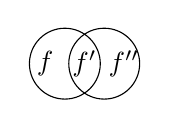
\begin{tikzpicture}\draw (0,0) circle (0.45); \draw (0.5,0) circle (0.45); \node at (-0.25,0) {$f$}; \node at (0.25,0) {$f'$}; \node at (0.75,0) {$f''$};\end{tikzpicture}\end{diagramblock}}

(${}^{13}$!)   This is nonsense again for n $\geqslant$1,  see PS at the end of section 13.
\margin{Even this PS is still unaccurate, compare comments section 18.}

(${}^{14}$!)   Same mistake as \xout{in} the one noticed in the previous note.  The
fibered products exist in $\underline{C}$\hand{$_{\bullet}$} only,  and \uline{these} should be preserved by the
functors under consideration. Thus the "universal problem" \deleted{\xout{has}} has to be
rephrased somewhat ...

(${}^{15}$)   I guess they are not equivalent,  even when restricting to objects
which are groupoids (i.e. so-called Gr-categories).

(${}^{16}$)  An object of M is called fibrant (resp. trivial) it the map from it
to the final object is fibrant (resp. a weak equivalence).

(${}^{17}$)   This seems doubtful,  unless all objects of M are fibrant (which is
true for the most familiar cases I was having in mind).  But even assuming
this,  we still need a unicity statement (in a suitable sense) for the
functors  $\underline{B}_{o}$\hand{$\to$} M  thus obtained,  in order to be sure that the correspon-%
ding functors  M\hand{$\to$}(Ho) are all canonically isomorphic.  These kind of
questions may be viewed as closely related to the question of existence
(and unicity) of ``test functors'' for a given test category A (here,  the
category of ``standard hemispheres'' \hand{\unsure{$\bigcirc$}}) into a given asphericity or con-%
tractibility structure,  as discussed in section 90 (without yet getting
there \xout{\unsure{the}}\inserted[typed]{any} clear-cut handy existence and unicity theorems \deleted{which are}\inserted{as are} to
be \xout{hoped} hoped for). \inserted{In my notes,} \over{T}{t}he set-up of asphericity and contractibility struc-%
tures,  which has been worked out in the months following,  has been gra-%
dually replacing Quillen's approach to homotopy models.  (I'll have to co-%
me back in due course to the\hand{/}question of the relationship between the two
approaches,  which deserves to be understood.)

(${}^{18}$)  The word ``gerb'' here stands \xout{for} as a ``translation'' of the French
word ``gerbe'',  as used in Giraud's book on non commutative cohomological
algebra.  With the terminology of next section,  we would call it rather
a ``stack of groupoids'' or  ``Gr-stack'' (with a specification by n or $\infty$ if
needed !).

(${}^{19}$!)  This is false,  as seen below.

(${}^{20}$\xout{\unsure{1}}!)  This description is dubious,  as it may give categories $\underline{C}_{n}$ which
are larger than the ones we want.

(${}^{21}$!)  It seems dubious however that the mere category structure of $\underline{C}$ will
allow us to recover the \xout{\unsure{the}} ``primitive'' subcategory $\underline{C}_{o}$ ,  and it looks sa-%
fer to add the latter as an extra structure to $\underline{C}$ .

\mspage{79}

\clearpage
% Pursuing Stacks (cotes 134-2 to 134-8): archive cote 134-2, site page 80 (PDF page 81).
% notes to ch. I. Draft compared: ps1.tex:1188-1193 ; ps1.tex:1193-1195 ; ps1.tex:1205-1205.
% AI-transcribed by Claude Opus 5.5 (claude-opus-5-5, adaptive thinking, effort high), Message Batches API, batch ps1 (msgbatch_01Rv5hCaNTtUt4JHx1yqoHPL), 2026-11-12; not yet checked by eye.
\scanpage{134-2/80}
\mspage{64}

(${}^{22}$) For the notion of a ``\uline{lien}'' \hand{(}or ``tie''\hand{)}\hand{,} wh\over{a}{\unsure{i}}ch is one of the main in-%
gredients of the non commutative cohomology panoply of Giraud's theory, I
refer to his book (Springer\hand{,}Grundlehren 179, 1971).\hand{/}\inserted{A} \uline{Picard category}\xout{xx}
\margin{$\otimes$,}\inserted[typed]{is a groupoi} \xout{\unsure{is a category is}} endowed with an operation \inserted{$\otimes$} \deleted{\illegible{1}} \xout{which makes it resemble to an}
together with associativity, unity and commutativity data for this opera-%
tion, which make it resemble to a commutative group. \inserted{A} ``\uline{Champ\xout{x} de Picard}''
\hand{(}or ``Picard stack\deleted{\unsure{s}}''\hand{)} \inserted[typed]{is} \xout{are} defined accordingly, by relativizing over an arbi-%
trary space or topos (replacing the groupoid by a stack of groupoids over
this topos). The necessary \hand{``}general\deleted{\unsure{ly}} nonsense\hand{''} on these \inserted{notions} is \unsure{developped|developed} rathe
carefully in an exposé of Deligne in SGA 4 (SGA 4 XVIII 1.4). In this
letter to Larry Breen, I am assuming ``known'' the notion of an n-stack
(for $n$\over{$=2$}{\unsure{$\leq 3$}} at any rate), and the corresponding notion of (strict) \deleted{n-}\uline{Picard}
\inserted{n-}\uline{stack}, which should be describable (as was explained in Deligne's notes
in the case n=1) by an n-truncated chain complex in the category of abeli-%
an sheaves on X (viewed mainly as an object of the relevant derived catego-%
ry). The ``strictness'' condition on usual Picard stacks refers to the
restriction that the commutativity isomorphism within an object $L$\hand{$\otimes$}$L'$ , \xout{wh}
when L=L', should reduce to the identity. It is assumed (without further
explanation) that the condition carries over in a natural way to Picard
n-stacks, in such a way as to allow an interpretation of these by truncate\hand{d}
objects in a suitable derived category, as hinted above.

(${}^{23}$) When M is any abelian sheaf on a topos, \inserted{(the ``Mac-Lane resolution'')} X(M) is a certain canoni-%
cal \inserted{left} resolution of M by sheaves of $\underline{Z}$-modules which are ``free'', and more
specifically, which are finite direct sums of sheaves of the type
$\underline{Z}^{(T)}$ , where T is any sheaf of the type $M^{n}$ (finite product of copies of
M ). This canonical\deleted{ly} construction was introduced \deleted{first} by MacLane\inserted{(for abelian groups)}, and
gained new popularity in the French school of algebraic geometry and homo-%
logical algebra in the late sixties, because \xout{in case M is described by}
\xout{some abelian group scheme over a ground} it gives a very handy way to rela-%
te the $\mathrm{Ext}^{i}(M,N)$ invariants (when N is another abelian sheaf on X) to
the \xout{\unsure{sp}} ``spacial'' cohomology of M (i.e. of the induced topos $X_{/M}$\hand{)} with
coefficients in N.

(${}^{24}$) Reflecting on the ``right'' version of the provisional Verdier notion
of a \inserted[typed]{triangulated} \xout{derived} category (which was supposed to describe adequately\deleted{\unsure{,}} the \inserted{relevant} inter-%
nal structure of the derived categories of abelian categories) is part of
my present program for the notes on Pursuing Stacks, and will be the main
task in one of the chapters of volume two. \deleted{Compare} \inserted{For} \hand{some indications along}
\hand{these lines, see also section \unsure{69} (sketching the basic notion of a ``\uline{derivator}'').}

(${}^{25}$) As was seen in section 9, ``uniqueness'' here has to be understood in

\margin{80}

\clearpage
% Pursuing Stacks (cotes 134-2 to 134-8): archive cote 134-2, site page 81 (PDF page 82).
% notes to ch. I. Draft compared: ps1.tex:1385-1387 ; ps1.tex:1394-1406 ; ps1.tex:1597-1600 ; ps1.tex:1621-1621 ; ps1.tex:1623-1648.
% AI-transcribed by Claude Opus 5.5 (claude-opus-5-5, adaptive thinking, effort high), Message Batches API, batch ps1 (msgbatch_01Rv5hCaNTtUt4JHx1yqoHPL), 2026-11-12; not yet checked by eye.
\scanpage{134-2/81}
\mspage{65}

\inserted{a} considerably wider sense than I expected,  when writing this letter to
Larry Breen.  It now appears that the whole theory of stacks of groupoids
will depend on the choice of a ``coherator'' $\underline{C}$ , as seen in section 13.

($^{26}$)\quad Tim Porter pointed out to me that ``Dold Puppe'' is an \inserted{in}accurate name
for this basic theorem,  which should be called \uline{Dold-Kan theorem}.

($^{27}$)\quad As was pointed out to me by Ronnie Brown,  this structure was
already well-known to J.H.C. Whitehead,  under the name of ``crossed modu-%
le\xout{\unsure{s}}'',  and extensive use and extensive generalizations of this notion
(in quite different directions from those I was having in mind,  in
terms of Gr-stacks over an arbitrary topos) have been made by him and
others.  With respect to the question on next page,  of generalizing this
notion of ``non commuative chain complex'' from length one to length two,
Ronnie says there is a work in preparation by D. Conduché `` Modules croi-%
sés généralisés de longueur 2 '' .

($^{28}$)\quad Tim Porter pointed out to me that work on étale tubular neighbour-%
hoods was done by D.A. Cox ; ``Algebraic tubular neighbourhoods I,II',
Math. Scand. 42 (1978)  211-228, 229-242.  I've not seen yet this work,
and can't say therefore whether it meets the rather precise expectations
I have for a theory of tubular neighbourhoods,  for the needs of a dévis-%
sage theory of stratified schemes (or, more generally, stratified topoi).

($^{29}$)\quad This is the typical game \xout{\unsure{to be}} embodied in the ``derivator'' associa\xout{\unsure{te}}%
\hand{-}ted to the theory (Hot) of usual homotopy types (compare section 69).

($^{30}$)\quad Some more details on this program are outlined in \hand{``}\uline{Esquisse d'un
Programme}\hand{''}(section 5),  in \uline{Réflexions} \uline{Mathématiques} 1 .

($^{31}$)\quad I was informed by knowledgeable people soon later that the answer is
well known to be negative,  by working with ``rational homotopy types''
(the cohomology of which is made up with vector spaces over $\underline{Q}$). It is well
known indeed that a 1-connected rational homotopy type is \uline{not} known from
it\unsure{\deleted{'}}s rational cohomology ring alone,  which \deleted{is supposed (I confess I did'nt
check) to} contain\hand{s} already all the information I was contemplating\deleted{\unsure{.(*)}}\inserted{\deleted{\illegible{1}} \deleted{(*)} At least \inserted{this is so} if we assume that \deleted{\unsure{the}} $H^i(X)$ is of finite dimension over $\mathbb{Q}$ for all $i$. But is there a counterexample still when $X$ is a homotopy type ``of finite type'' ?}

($^{32}$)\quad This \inserted[typed]{``problem'' is met with by the notion of a ``derivator''}\xout{is the non \unsure{commutative} version of the similar problem} , which
``was in the air'' already by the late sixties,  but was never developped \deleted{\illegible{1}}
(instead even derived categories became tabu in the seventies ...). Compare
with note ($^{24}$).

\margin{81}

\clearpage
% Pursuing Stacks (cotes 134-2 to 134-8): archive cote 134-3, site page 1 (PDF page 2), typescript page 1.
% typescript. Draft compared: ps2.tex:1-67.
% AI-transcribed by Claude Opus 5.5 (claude-opus-5-5, adaptive thinking, effort high), Message Batches API, batch ps1 (msgbatch_01Rv5hCaNTtUt4JHx1yqoHPL), 2026-11-12; not yet checked by eye.
\scanpage{134-3/1}
\margin{1}
\mspage{1}

Reflections on homotopical algebra

27.2.83.

\margin{\unsure{\#}} The following notes are the continuation of the reflection star-%
ted in my letter to Daniel Quillen written previous week (19.2 - 23.2),
which I will cite by (L) (``letter''). I begin with some corrections and
comments to this letter.

\hand{14}. Homotopical algebra can be viewed as being concerned mainly with
the study of spaces of continu\xout{\unsure{o}}ous \xout{functions} \inserted{maps between spaces} \deleted{and their}\inserted{, and the} algebraic analo-%
gons, \inserted{of these} \xout{\illegible{1}} with a special emphasis on homotopies between such \xout{functions}\inserted[typed]{maps},
homotopies between homotopies etc. The kind of restrictive properties
imposed on \deleted{functions} \inserted{the maps under consideration} is exemplified by the typical example when deman-%
ding that the \xout{functions} \deleted{considered} \inserted[typed]{maps} should be extensions, or liftings, of
a given \xout{function} map. \deleted{It} \inserted{Homotopical algebra} is not \inserted{directly} suited for the study of spaces of homeo-%
morphisms, spaces of immersions, of embeddings, of fibrations etc
- and it seems that the \deleted{latter} study \inserted{of such spaces} has not really yet taken off the
ground. Maybe the main obstacle here lies in the wildness phenomena,
which however, one feels, makes a wholly artificial difficulty, stem-%
ming from the particular way by which topological intuition has been
mathematically formalized, in terms of the basic notion of topological
spaces and continuous maps between them. This transcription, while
adequate for the homotopical point of view, and partly adequate too
for the use of analysts, is rather coarsely unad\hand{e}quate, it seems to me,
in most other geometrico-topological contexts, and particularly so when
i\over{\unsure{l}}{t} comes to studying spaces of homeomorphisms, immersions etc (in all
those questions when \xout{the} ``isotopy'' is replacing the rather coarse homo-%
topy relation), as well as for a study of stratified structures, when
it becomes undispensable to give intrinsic and precise meaning to such
notions as tubular neighbourhoods etc. For a structure theory of strati
fications, it turns out,\inserted[typed]{(somewhat surprisingly maybe)} that even the somewhat cumbersome context of
\xout{pre}topoi and \unsure{pro-topoi|pretopoi} is better suited than topological spaces, and mo\unsure{re}
over directly applicabl\unsure{e} to unconventional contexts such as étale topo-%
logy of schemes, where the conventional transcription of topological
intuition in terms of topological spaces is quite evidently breaking
down. To emphasize one point I was making in (L,p.1), it seems to me
that this breakdown is almost as evident in \xout{\illegible{1}} isotopy questions\hand{,} or
for the needs of a structure theory of stratified ``spaces'' (whatever we
mean by ``spaces'' ...). \deleted{and} \over{i}{I}t is a matter of amazement to me that this
breakdown has not been clearly noticed, and \inserted{still less} overcome by \xout{axsuitable}
working out a more suitable transcription of topological objects and

\clearpage
% Pursuing Stacks (cotes 134-2 to 134-8): archive cote 134-3, site page 2 (PDF page 3), typescript page 2.
% typescript. Draft compared: ps2.tex:55-115.
% AI-transcribed by Claude Opus 5.5 (claude-opus-5-5, adaptive thinking, effort high), Message Batches API, batch ps1 (msgbatch_01Rv5hCaNTtUt4JHx1yqoHPL), 2026-11-12; not yet checked by eye.
\scanpage{134-3/2}
\margin{2}
\mspage{2}

topological intuition,  by the people \inserted{primarily} concerned,  namely the topologists.
T\over{h}{h}e need of eliminating wildness phenomena has of course been felt repea-%
tedly,  and (by lack of anything better maybe,  or rather by lack of any
attempt of a systematic reflection on what \uline{was} needed) it was supposed
to be met by the notion of piecewise linear structures.  This however
was falling from one extreme into another  -  from a structure species
with vastly too many maps between "spaces",  like a coat vastly too wide
and floating around in a million wild wrinkles,  to one with so few
(not even a quadratic map from $\underline{R}$ to $\underline{R}$ is allowed !) that it feels like
too narrow a coat,  bursting \inserted{apart} on all edges and ends.  The main defect
here,  technically speaking,  seems to me the fact that \deleted{numerical}\inserted{$\mathbb{R}$-valued} piece-%
wise linear functions are not stable under multiplication,  and as a geo-%
metric consequence of this,  that when contracting a compact p.l. sub-%
space of a (compact, say) piecewise linear space into one point,  we do
not get on the quotient \xout{\unsure{structurexx}} \hand{space} a natural p.l. structure.  This
alone should have sufficed,  one might think,  to eliminate the piecewi-%
se linear structure species as a reasonable candidate for \xout{eliminating}
``doing topology'' wi\over{th}{th}out wildness empidements  -  but strangely enough,
it seems to be hanging around till this very day !

\margin{(15.)}15.  But my aim here is not to give an outline of foundations  on ``tame
topology'',  but rather to fill some foundational gap\deleted{s} in homotopy theory\hand{,}
more specifically in homotopical algebra.
\margin{pas à la ligne}The relative success \deleted{here} in th\over{e}{e} \deleted{\unsure{x topic,}}  homotopical approach to topo-%
logy is probably closely tied to the well known fact (\over{b}{B}rouwers starting
point as a matter of fact,  when he introduced the systematics of trian-%
gulations)  that every continuous map between triangulated spaces can be
approximated by simplicial maps.  This gave rise,  rather naturally,  to
the hope expressed in the \hand{``}Hauptvermutung\hand{''}  -  that two homeomorphic trian%
gulated spaces admit isomorphic subdivisions,  a hope that finally proved
a delusion.  With a distance of two or three generations,  I would
comment on this by saying that this negative result was the one to be
expected,  once it has become clear that neither of the two structure
species one was comparing,  namely topological spaces and triangulated
spaces,  was adequate for expressing what one is really after  -  namely
an accurate mathematical transcription,in terms of ``spaces'' of some kind
or other, of some vast and deep and misty and ever transforming \unsure{mase|mass} of
intuitions in our psyche,  which we are referring to as ``topological''
\margin{\unsure{$\Pi$}}intuition\deleted{s}\hand{$(^1)$}. There \uline{is}  something positive though,  definitely,  which
can be viewed as an extremely weakened version of the Hauptvermutung,
namely the fact that topological spaces on the one hand,  and semi-simp-%
plicial sets on the other,  give rise,  by a suitable ``localization''

\clearpage
% Pursuing Stacks (cotes 134-2 to 134-8): archive cote 134-3, site page 3 (PDF page 4), typescript page 3.
% typescript. Draft compared: ps2.tex:104-159.
% AI-transcribed by Claude Opus 5.5 (claude-opus-5-5, adaptive thinking, effort high), Message Batches API, batch ps1 (msgbatch_01Rv5hCaNTtUt4JHx1yqoHPL), 2026-11-12; not yet checked by eye.
\scanpage{134-3/3}
\margin{3}
\mspage{3}
pro\unsure{c}ess (formally analogyous to the passage from \xout{chain} categories of
chain complexes to the corresponding derived categories), to essentially
``the same'' (up to \unsure{equivalence})\hand{|}``homotopy category''. One way of describing
it is via topological spaces which are not ``too wild'' as objects (the
\unsure{C.W.-spaces}), \deleted{and \xout{maps}}\inserted[typed]{morphisms} being homotopy classes of continuous maps. The
other is via semi-simplicial sets, taking for instance Kan complexes as
objects, and again homotopy classes of ``maps'' as morphisms. The first
description is the one most adapted to direct topological intuition,
as long a\over{s}{t} least as no more adequate notion than ``topological spaces'' is
at hand. The second has the advantage of being a purely algebraic
description, with rather amazing conceptual simplicity moreover. In
terms of the two basic sets of algebraic invariants of a space which hav\unsure{e}
turned up so far, namely cohomology (or homology) on the one hand, and
homotopy gro\hand{u}ps on the other, it can be said that the description via
topological spaces is adquate for direct \deleted{description}\inserted{computation} of neither \inserted{co}homology
nor homotopy groups, whereas the description via semi-simplicial sets i\hand{s}
fairly adequate for \deleted{description}\inserted{computation} of cohomology groups (taking simply the
ab\unsure{e}lianization of the semi-simplicial set, which turns out to be a
chain complex, and taking it's homology and cohomology groups). The
same can be said for the alternative algebraic description of homotopy
types, using cubical complexes instead of semi-simplicial ones, which
were introduced by Serre\hand{,} as they were better suited, it seems,\hand{(2),} for the
study of fibrations and \inserted{of} the homology and cohomology spectral sequences
relative to these. One somewhat surprising common feature of those two
standard algebraic descriptions of homotopy types, is that neither is
any better adapted for a direct desc\hand{r}iption of homotopy groups than the
objects we started with, namely topological spaces. This is all the
more remarkable as it is the homotopy groups really, rather than the
cohomology groups, which are commonly viewed as \uline{the} basic inveriants
in the homotopy point of view, sufficient e.g. for testing whether a
given map \xout{given} is a ``weak equi\uline{valence''} namely gives rise to an isomor-%
phism in the homotopy \uline{category.}\hand{||}\margin{$\lrcorner$||} It is here of course that the point of
view of ``stacks'' (``champs'' in French) of (L) (previously called ``$\infty$-\hand{grou-}
\unsure{poïdes|poïds}'' in the beginnings of the reflections of (L)) sets in. These
presumably give rise to a ``category of models'' and from there, to the
usual homotopy category, in much the same way as topological spaces
or simplicial (or cubical) complexes, thus yielding a third main des-%
cription\inserted{of homotopy types,}, and corresponding wealth of algebraico-geometric intuitions\over{,}{.}
\deleted{of homotopy types,} Moreover, stacks are ideally suited for expressing
the homotopy groups, in an even more direct way than simplicial comple-%

\clearpage
% Pursuing Stacks (cotes 134-2 to 134-8): archive cote 134-3, site page 4 (PDF page 5), typescript page 4.
% typescript. Draft compared: ps2.tex:148-209.
% AI-transcribed by Claude Opus 5.5 (claude-opus-5-5, adaptive thinking, effort high), Message Batches API, batch ps1 (msgbatch_01Rv5hCaNTtUt4JHx1yqoHPL), 2026-11-12; not yet checked by eye.
\scanpage{134-3/4}
\margin{4}
\mspage{4}

xes allow description of homology and cohomology groups.  As a matter of
fact,  the description is formally analoguous,  and nearly identi\unsure{d|c}al, to
the description of the homology groups of a chain complex  -  and it
would seem therefore that stacks (more specifically,  Gr-stacks) are
in a sense the \uline{closest possible} \inserted[typed]{\uline{non commutative}} \uline{generalization of}  \uline{chain complexes},
the homology groups of the chain complex becoming the homotopy groups
of the ``non commutative chain complex'' or stack.

It is well understood,  since Dold-Puppe\hand{${}^{(3)}$,} that chain complexes
form a category equivalent to the category of abelian group objects in
the category of semi-simplicial sets,  or equivalently, \inserted{to} the category of
semi-simplicial abelian groups.  By this equivalence,  the homology
groups of the chain complex are identified with the \uline{homotopy} groups of
the corresponding homotopy type.  As for the \xout{cxxxxx} homology and cohomolo%
\hand{-}gy groups of this homotopy type,  their description in terms of the
chain complex we started with is kind of delicate (I forgot all about it
I am affraid !).  A fortiori, when a homotopy type is described in terms
of a stack,  i.e. a ``non commutative chain complex'',  there is no immedi-%
ate way for describing its homology or cohomology groups  in terms of
this structure\hand{(*)}. What probably should be done,  is to define \inserted{first} a \uline{nerve}
\margin{3.5. This is an error\unsure{;} it appeared soon after that the cohomology can be expressed much in the same way as for \unsure{simplicial} or \unsure{cubical} complexes, using the ``nerve'' and ``forgetting'' \unsure{the structure} of the stack (i.e. \unsure{part} of the ``primitive'' structure.}
functor  from stacks to semi-simplicial sets  (generalizing the familiar
nerve functor defined o\over{f}{n} the category of categories),  and define homolo-%
gy invariants of a stack via those of the associated semi-simplicial set
(directly suited for calculating these).

\margin{16.}
These reflections on the proper place of the notion of a stack with-%
in standard homotopy algebra  are largely a posteriori  -  the clues the\hand{y}
give are surely not so strong as to \inserted[typed]{give an} \xout{\unsure{be}} imperative feeling for the need
of developping this new approach to the homotopy category.  Rather,  the
imperative feeling comes from the \xout{needs of} intuitions tied up with non
commutative  cohomological algebra over topological spaces,  and more ge\unsure{n}%
\hand{-}nerally over topoi, in the spirit of Giraud's thesis,  where a suitable
formalism for non commutative H$^{i}$'s for  i=0,1 or 2 is developped.  He
develops in extenso the notion of stacks,  we should rather say now
1-stacks,  over a topos,  constantly eluding (and for very understandable
reasons !) the notion of a \xout{two} 2-stack,  appearing closely on the heels
of the 1-stacks.  Keeping in mind that 0-stacks are just ordinary
sheaves of sets\hand{,}  on the space or the topos considered,  the hierarchy o\hand{f}
increasingly higher and more sophisticated notions of 0-stacks, 1-stacks,
2-stacks etc,  which will have to be developped over an arbitrary topos,
just parallel\hand{s} the hierarchy of corresponding notions over the one-point

\clearpage
% Pursuing Stacks (cotes 134-2 to 134-8): archive cote 134-3, site page 5 (PDF page 6), typescript page 5.
% typescript. Draft compared: ps2.tex:197-255.
% AI-transcribed by Claude Opus 5.5 (claude-opus-5-5, adaptive thinking, effort high), Message Batches API, batch ps1 (msgbatch_01Rv5hCaNTtUt4JHx1yqoHPL), 2026-11-12; not yet checked by eye.
\scanpage{134-3/5}
\mspage{5}

\margin{5}
space, namely sets\inserted{(= 0-stacks)}, categories (or 1-stacks), 2-categories etc. Amon\unsure{g}
these structures, those generalizing groupoids among categories, \inserted{namely}
Gr-stacks of various orders n, play a significant role, especially
for the description of homotopy types, but equally for a non-commutati\hand{ve}
``geometric'' interpretation of the cohomology groups $H^i(X,F)$ of arbitra-%
ry dimension (or ``order), of a topos X with coefficients in an abelian
sheaf F. The reflections in (L) therefore were directly aimed at get-%
ting a grasp on a definition of such Gr-stacks, and whereas it seems to
me to have come to a concrete starting point for such a definition, a
similar reflection for defining \inserted{just} stacks \xout{\illegible{1}} rather than Gr-stacks,
is \inserted{still} lacking\unsure{\over{,}{.}} \xout{and} \over{t}{T}his is \inserted{one} among the manyfold things I have in mind whi\over{he}{le}
sitting down on the present reflections.

Thus \uline{n-stacks}, \uline{relativized over a topos to ``n-stacks over X''}, \uline{are}
\uline{viewed primarily as the natural ``coefficients'' in order to do} \inserted{[non commutative]}\uline{(co)homolo-}%
\uline{gical algebra of dimension} \over{$<$}{$\le$} n over X. The ``integration'' of such
coefficients, in much the same spirit as taking objects $R\hand{\Gamma}F_{\hand{\ast}}$ (\inserted{with $R\Gamma$} the deri-%
ved functor of the sections functor \inserted{$\Gamma$}\hand{)} for complexes of abelian sheaves $F_{\hand{\ast}}$
on X, is here merely the trivial operation of taking sections, namely
the``value'' of the n-stack on the final object of X (or of a representa-%
tive site of X, if X is described in terms of a site). The result of
integration is again an n-stack, whose homotopy \xout{\illegible{1}} groups (with a
dimension shift of n) should be viewed as the cohomology invariants
$H^i(X,F_{\hand{\ast}})$ , where $F_{\hand{\ast}}$ now stands for the n-stack rather than for a com-%
plex of abelian sheaves\hand{(5)}.In my letters (two or three) to Larry Breen in
1975, I develop some heuristics along this point of view, with constant
reference to various geometric situations (mainly from algebraic geome-%
try), providing the motivations. The one motivation maybe which was
the strongest, was the realization that the classical Lefschetz theorems
about comparison of homology and homotopy invariants of a projective
variety, and a hyperplane section - once it was reformulated suitably
so as to get rid of non-singularity assumptions, replaced by suitable
assumptions on cohomological ``depth'' - could be viewed as comparison
statements of ``cohomology'' with coefficients in more or less arbitrary
\uline{stacks}\hand{(6)}.This is carried through completely, within the th\hand{e}n existing
conceptual framework restricted to 1-stacks, in the thesis of Mme Ray-%
naud, a beautiful piece of work. There seems to me to be overwhelming
evidence that her results (maybe her method of proof too ?) should gener-%
lize \over{to}{in} the context of non commutative cohomological algebra of arbitra-%
ry dimension, with a suitable \xout{notion}\inserted[typed]{property} of ind-finiteness as the unique

\clearpage
% Pursuing Stacks (cotes 134-2 to 134-8): archive cote 134-3, site page 6 (PDF page 7), typescript page 6.
% typescript. Draft compared: ps2.tex:241-296.
% AI-transcribed by Claude Opus 5.5 (claude-opus-5-5, adaptive thinking, effort high), Message Batches API, batch ps1 (msgbatch_01Rv5hCaNTtUt4JHx1yqoHPL), 2026-11-12; not yet checked by eye.
\scanpage{134-3/6}
\margin{6}
\mspage{6}
restriction on the coefficient stacks under consideration.

\xout{Workingxoutxaxtheoryxof} Technically speaking, $\infty$-stacks are the
common denominator of n-stacks for arbitrary n, in much the same way as
n-stacks appear both as the next-step generalization of(n-1)-stacks
(\inserted[typed]{the former}forming a category which admit\hand{s} the category of (n-1) stacks as a full
subcategory), and as the most natural "higher order structure" appearin
% NOTE: the right edge of the scan cuts off the end of this line ("appearin...")
on the category of all \xout{nxstacks} (n-1)-stacks, \inserted{(and on} \xout{xxxx} various \unsure{analoguous|analogous} ca-
tegories whose objects are (n-1)-stacks subject to some restrictions or
endowed with some extra structure\hand{)}. I'll have to make this explicit in
due course. For the time being, when speaking of ``stacks'' or ``Gr-stacks\hand{''}
it will be understood (unless otherwise specified) that we are dealing
with the infinite order notions, which encompass\hand{\unsure{es}} the finite ones.

Working out a theory of stacks over topoi, as the natural founda-%
tions of non commutative cohomological algebra, would amount among
others to rewrite Giraud's book within this considerabl\over{e}{y} wider framework
% NOTE: the right edge of the scan cuts off the end of this line after "framework"
Of course, this mere prospect would'nt be particularly exciting by it-%
self, if it did not appear as something more than grinding through an
unending exercise of rephrasing and reproving known things, replacing
everywhere n=0,1 or 2 by arbitrary n. I am convinced however that there
is a lot more to it - namely the fascination of gradually discovering
and naming and getting acquainted with presently still unknown, unnamed,
mysterious structures. As is the case so often when making a big step
backwards for gaining new perspective, there is not merely a quantitati
ve change (from n\hand{$\leqslant$}2 to arbitrary n say), but a qualitative change in
scope and depth of vision. One such step was already taken I feel by
Daniel Quillen and others, when realizing that homotopy constructions
make sense not only in the usual homotopy category, or \inserted{in} one or the other
categories of models which give rise to it, but in more or less arbitra
\margin{-}ry categories, by working with semi-simpli\over{\unsure{ci}}{ci}al objects \over{\unsure{of}}{in} these. The
step I am proposing is of a \inserted{somewhat} different type. \uline{The notion of a stack}
\uline{here appears as the unifying} \inserted[typed]{concept}\xout{notion} \uline{for a synthesis of homotopical alge-}%
\uline{bra}, \uline{and non commutative cohomological algebra}. This$_{\text{x}}$ \xout{Ixfxxxx} (rather
than \inserted[typed]{merely} furnishing us with still another description of homotopy types,
more convenient for expression of the homotopy groups) se\over{\unsure{ms}}{ems} to me the
real ``raison d'être'' of the notion of a stack, and the main motivation
for pushing ahead a theory of stacks.

\clearpage
% Pursuing Stacks (cotes 134-2 to 134-8): archive cote 134-3, site page 7 (PDF page 8), typescript page 7.
% typescript. Draft compared: ps2.tex:281-343.
% AI-transcribed by Claude Opus 5.5 (claude-opus-5-5, adaptive thinking, effort high), Message Batches API, batch ps1 (msgbatch_01Rv5hCaNTtUt4JHx1yqoHPL), 2026-11-12; not yet checked by eye.
\scanpage{134-3/7}
\mspage{7}

\margin{7}

\margin{16'.} 16.\hand{\deleted{\unsure{bis}}} One last comment before diving into more technical matters. Without
even climbing up the ladder of increasing sophistication, leading up
to $\infty$-stacks, there is on the very first step, namely with just usual
categories, the possibility of describing arbitrary homotopy types.
Namely, there are two natural, well known ways to associate to a cate-%
gory C (I mean here a ``small'' category, belonging to \deleted{a}\inserted{the} given universe
we are working in) some kind of topological object, and hence a homotopy
type. One is by associating to C the topos $\overset{\hand{$\wedge$}}{C}$ or Top(C), the sheaves on
which are just the presheaves on C, namely arbitrary contravariant func-%
tors from C to (Sets). The other is through the nerve functor\inserted{(7)}, associa-%
ting to C a semi-simplicial set - and hence, if this suits us better,
a topological space, by taking the geometrical realization. \over{b}{B}y a con-%
struction of Verdier, any topos and therefore Top(C) gives rise canoni-%
cally to a pro-object in the category of semi-simplicial sets, and hence
by ``localization'' to a pro-object in the homotopy category (namely a
\hand{``}pro-homotopy type\hand{''} in the terminology of Artin-Mazur). In the same way,
the nerve $\underline{N}$(C) gives rise to a homotopy type - and of course the two
(pro)-homotopy types thus obtained coincide essentially, and may be
called \uline{the} homotopy type of C. When C is a groupoid, we get merely
a 1-truncated homotopy type, namely with homotopy groups \hand{$\pi$}$_n$ which va-%
nish for n\hand{$\geqslant$}2, or equivalently, with connected components (correspon\xout{d}d-%
ding of course to connected components of C) K(\hand{$\pi$},1) spaces. This had
led me \inserted{at one moment} in the late sixties to \inserted{hastily} surmise that even for arbitrary C, we got
merely such sums of K(\hand{$\pi$},1) spaces (namely, that the homotopy type of C
does not change when replacing C by the universal enveloping groupoid,
deduced from C by \xout{xxxxx} making formally invertible all it's arrows).
As Quillen pointed out to me, this is definitely not so - indeed,
using categories, we get (up to isomorphism) arbitrary homotopy types.
This is achieved, I guess, using the \inserted[typed]{left} adjoint functor \inserted{N'} from the
inclusion functor
\[ \begin{diagramblock}\begin{tikzcd} \text{(Cat)} \ar[r, hook, "\underline{N}"] & \text{(Ss sets)} \end{tikzcd}\end{diagramblock} \]
which is fully faithful \hand{(}the adjoint functor being therefore a localiza-%
tion functor\hand{)}, and showing that for a semisimplicial set K, the natural
\margin{\unsure{5.3.} This is false, see \unsure{§24} below (p. 21-22) (!8)}
map
\[ \deleted{\illegible{1}}\ K \hand{$\longrightarrow NN'(K)$} \]
is a weak equivalence\deleted{\illegible{1}}\hand{\unsure{;|,}} or what amounts to the same, that the set of
arrows in (Ss sets) by which we localize in order to get (Cat) \hand{(}namely
those transformed into invertible arrows by $\underline{N}$') \deleted{are} is made up with
weak equivalences only\inserted{(!8)}. This would imply that we may reconstruct the
usual homotopy category, up to equivalence, in terms of (Cat), by

\clearpage
% Pursuing Stacks (cotes 134-2 to 134-8): archive cote 134-3, site page 8 (PDF page 9), typescript page 8.
% typescript. Draft compared: ps2.tex:335-384.
% AI-transcribed by Claude Opus 5.5 (claude-opus-5-5, adaptive thinking, effort high), Message Batches API, batch ps1 (msgbatch_01Rv5hCaNTtUt4JHx1yqoHPL), 2026-11-12; not yet checked by eye.
\scanpage{134-3/8}
\margin{8}
\mspage{8}

just localizing (\over{C}{C}at) with respect to weak isomorphisms, namely func-%
tors $C$ \hand{$\to$} $C'$ inducing an isomorphism between the corresponding homoto-%
py types. Pushing a little further in this direction, one may conjectu%
re that (Cat) is a \hand{``}closed model category,\hand{''} whose weak equivalences are
the functors just specified, and whose cofibrations are just functors
which are injective on objects and injective on arrows.\hand{(19).}

The fact that categories are suitable objects for defining \inserted{arbitrary} homotopy
types is quite remarkable, and one moreover it seems which has not found
it's way still into the minds of topologists o\over{f}{r} homotopists, with only
few exceptions I guess. These objects are extremely simple and familiar
to most mathematicians; what is somewhat more sophisticated is the
process of localization towards homotopy types, or equivalently, the
explicit description of weak equivalences, within the framework of
\inserted{usual} category theory. This would amount more or less to the same as descri-%
bing the homotopy groups of a category, which does not seem any simpler
than the same task for its nerve. As for the cohomology invariants, which
can be interpreted as the left derived functors of the $\underset{\hand{$\leftarrow$}}{\lim}_{C}$ functor ,
or rather its values on particular presheaves (for instance constant
presheaves), they are of course known to be significant\hand{,} independently
of any particular topological interpretation, but they are not expressi%
-ble either in direct terms. (The most common computation for these is
again via the nerve of C.)

This situation suggests that for any \xout{w}natural integer n\hand{$\geq$}1, the
category of n-stacks can be used as a category of models for \inserted{the,} usual homo-%
topy category, in particular any n-stack gives rise to a homotopy type,
\xout{whilexthe} and up to equivalence we should get any homotopy type in this
way (for instance, through the n-category canonically associated to
any 1-category giving rise to this homotopy type). The homotopy types
coming from n-Gr-stacks, however, should be merely the n-truncated
ones, namely those whose homotopy groups in dimension \hand{$>$} n are zero.
\xout{Theyxappearx} Moreover, \xout{as} n-Gr-stacks appear as \inserted{([in some respects])} the most ad\unsure{\over{e}{e}}quate \margin{\illegible{1}}
algebraic structures for expressing n-truncated homotopy types, the
latter being deduced from the former, presumably, by the same process
of localization by weak equivalences. Moreover, in the context\deleted{s} of
n-Gr-stacks, the notions of homotopy groups and of weak equivalences
are described in a particularly obvious way. Thus, passing to the
limit case n=$\infty$ , it is $\infty$-Gr-stacks rather than general $\infty$-stacks
which appear as the neatest algebraic description of homotopy types.

\clearpage
% Pursuing Stacks (cotes 134-2 to 134-8): archive cote 134-3, site page 9 (PDF page 10), typescript page 9.
% typescript. Draft compared: ps2.tex:372-433.
% AI-transcribed by Claude Opus 5.5 (claude-opus-5-5, adaptive thinking, effort high), Message Batches API, batch ps1 (msgbatch_01Rv5hCaNTtUt4JHx1yqoHPL), 2026-11-12; not yet checked by eye.
\scanpage{134-3/9}
\margin{9}
\mspage{9}

These reflections suggest that there should be a rather impressive
bunch of algebraic structures,  each giving rise to a model category
for \inserted{the} usual homotopy category,  or in any case yielding this category by
localization with respect to a suitable notion of "weak equivalences".
T\unsure{\over{h}{h}}e"bunch"is all the more impressive,  if we remember that the notion
of a stack  (dropping now the qualification $n$ namely assuming $n=\infty$ )  is
not really a uniquely defined one,  but depends on the choice of a
"\uline{coherator}",  namely (mainly) a category $C$ satisfying certain require-%
ments,  which can be met in a vast variety of ways\hand{,} presumably.  T\unsure{\over{h}{h}}e con-%
struction of coherators is achieved in terms of universal algebra,
which seems here the undispensable Ariane thread not to get lost in
overwhelming messyness.  T\unsure{\over{h}{h}}e natural question which arises\inserted{here} (and which I
\margin{\unsure{$\lambda$} (10)}\uline{do not feel though like pursuing})\hand{\unsure{//}} is to give\inserted{in terms of universal algebra} some kind of caracterizati-%
on,  among all "algebraic" structures,  of those which give rise in
some specified ways\inserted[typed]{(including the known \unsure{ones|cases})} to a category of models say for usual homotopy theo-%
ry.

1\unsure{\over{8}{7}}.  When referring \deleted{\illegible{1}}\inserted{(section 15)} to the notion of a stack as a unifying concept
for homotopical algebra and non commutative cohomological algebra,  I
forgot to mention one signfficant \deleted{\illegible{1}}\inserted{observation} of Artin-Mazur along those li-%
nes\inserted{(\unsure{namely|messy}, unification)},  namely that (for ordinary homotopy types say) weak equivalences
(namely maps inducing isomorphisms for all homotopy groups)  can be ca-%
racterized as being those which induce isomorphisms on cohomology groups
\xout{\illegible{1}} of the spaces considered not only for constant coefficients,  but
also for \deleted{\xout{\illegible{1}}} arbitrary twisted coefficients on the target space,
including also the non commutative H$^{0}$ and H$^{1}$ for twisted \xout{\illegible{1}} (non commu%
% NOTE: the end of this line is at the right edge of the scan; a hyphen after "commu" may be cut off
tative) group coefficients.  This is ind\unsure{e|d}ed the basic technical result
enabling them,  from known results on etale cohomology\inserted[typed]{of schemes} (including non
commutative H$^{1}$'s) to deduce corresponding information on homotopy types.
Maybe however \deleted{that} their \hand{observation} has acted rather as a dissuasion for
developping higher non commutative cohomological algebra,  as it seeming-%
\margin{-}ly sa\over{\illegible{1}}{ys} that the non commutative H$^{1}$ ,  plus the commutative H$^{i}$\hand{\unsure{,}}'s, was
all that was needed to recover stringent information about homotopy
types.  In other words,  there was'nt too\xout{\illegible{1}} little in Giraud's book,
but rather,  too much !

\clearpage
% Pursuing Stacks (cotes 134-2 to 134-8): archive cote 134-3, site page 10 (PDF page 11), typescript page 10.
% typescript. Draft compared: ps2.tex:415-483.
% AI-transcribed by Claude Opus 5.5 (claude-opus-5-5, adaptive thinking, effort high), Message Batches API, batch ps1 (msgbatch_01Rv5hCaNTtUt4JHx1yqoHPL), 2026-11-12; not yet checked by eye.
\scanpage{134-3/10}
\mspage{\hand{10}}

28.2.

\over{\unsure{18}}{18}. I still have to correct a number of ``étourderies'' of (L). The
most persistent one, ever since page 8 of that letter, is about fiber
products in the coherator $\underline{C}_\infty$ , or, equivalently, amalgamated sums in
the dual category $\underline{B}_\infty$ . The ``correction'' I added in the last PS \inserted{(section 13)} \deleted{\unsure{p.11'}} is
still incorrect, namely it is not true \xout{thatxix} even in the subcategory
$\underline{B}_o$ of $\underline{B}$ that arbitrary binary amalgamated sums exist. I was mislead
by the interpretation of elements of $\underline{B}_o$ in terms of \inserted{(contractible)} spaces\hand{,} obtained
inductively by gluing together discs $D_n$ ($n \in \underline{N}$) via subdiscs, correspon-%
ding to the cellular subidivisions of the discs $D_n$ considered on p.7.
I was implcitly thinking of amalgamated sums of the type
\[ K \amalg_L M \quad , \]
where $L$ \hand{$\to$} $K$ and $M$ \hand{$\to$}\xout{x}$K$ are \uline{monomorphisms}, corresponding to the geometric
vision of embeddings - in which case the usual amalgamated sum in the
category of topological spaces is indeed contractible, wh\over{\unsure{at}}{ich} was enough
to make me happy. But I overlooked the existence of morphisms in $\underline{B}_o$
which are visibly no monomorphisms, such as $K \amalg_L K$ \hand{$\to$} $K$ the \unsure{codiagonal|codiaganal}
map, when $L$ \hand{$\to$}$K$ is a\xout{n} \inserted{strict} inclusion of discs\xout{x} . In any case, I will have
to come back upon the description of the categories $\underline{B}_o$ and it's dual $\underline{C}_o$ ,
and upon the definition of coherators, after the heuristic introduction
(L). It will be time then \inserted{too} to correct the mistaken description of $\underline{C}_{n+1}$
in terms of $\underline{C}_n$ , which I propose \inserted{there} \deleted{on p.11'}, yielding probably much too
big a subcategory of $\underline{C}$\xout{xxxx}\hand{$_\infty$} - the correct definition should make explicit
use of the \inserted{total} set A of \xout{xxxxxx} ``new'' arrows, by which $\underline{C}_\infty$ is described in
terms of universal algebra via $\underline{C}_o$ . Another étourderie the day before\hand{,}
\inserted{(section 7)} \deleted{p.7'}, is the statement that in a standart amalgamated sum, an\over{d}{y} inter-%
section of two \inserted{maximal} subcells is a subcell - which is seen to be false in
\margin{\unsure{[circle cut by a vertical arc, inner labels $t$, $f$, $f'$, $f''$, $s$; written beside it: $f\cup f''=f'\cup s\cup t$]}} th\over{e}{\unsure{e}} standard example\hand{.} \hand{\unsure{$\ell$}} \over{o}{O}f lesser import is the misstatement \inserted{(in section 2)} \deleted{on p.2'},
stating that the associativity relation for the operation \hand{$*_\ell$} should be
\xout{wherexfxf"xisxaxtwo-pointxspacex$\underline{S}_o$xxx} replaced by a homotopy arrow
$(\hand{\lambda}*\hand{\mu})*\hand{\nu} \to \hand{\lambda}*(\hand{\mu}*\hand{\nu})$. This is OK for \hand{$\ell$}=1 (primary composition), but
already for \hand{$\ell$}=2 does not make sense as stated, because the sources and
the targets of the two compositions to be compared are not equal, but
only homotopic. Here the statement should be replaced by one making
sense, with a homotopy ``making commutative'' a certain square, and accor\hand{\unsure{-}}%
dingly for cubes etc for higher order co\xout{mp}mpositions \hand{$\lambda *_\ell \mu$}, to give rea-%
sonable meaning to associativity. Anyhow, such painstaking explicita-%
tions of particular coherence properties (rather, coherence homotopies)
is kind of ruled out by the sweeping axiomatic description of the
kind of structure species we want for a ``stack'', at least\hand{,} I guess\hand{,} in

\clearpage
% Pursuing Stacks (cotes 134-2 to 134-8): archive cote 134-3, site page 11 (PDF page 12), typescript page 11.
% typescript. Draft compared: ps2.tex:470-531.
% AI-transcribed by Claude Opus 5.5 (claude-opus-5-5, adaptive thinking, effort high), Message Batches API, batch ps1 (msgbatch_01Rv5hCaNTtUt4JHx1yqoHPL), 2026-11-12; not yet checked by eye.
\scanpage{134-3/11}
\mspage{11}
a large part of the development of the theory of Gr-stacks.  A systematic
study of particular sets of homotopies is closely connected \inserted{of course} to an inves-%
\hand{(}tigation into irredundancy conditions which can be figured out for a
\inserted{general} coherator $\underline{C}$ .  This is indeed an interesting topic,  but I decided not
to get involved in this,  unless I am really forced to!

The basic notion which has been peeling out in the reflection (L)
is of course the notion of a coherator.  Concerning terminology,  it oc-%
cured to me that the dual category $\underline{B}_\infty$ to $\underline{C}_\infty$ is more suggestive in some
cases,  for instance because of the topological interpretation attached
to its objects,  and (more technically)  because of formal analogy of
the role of this category,  for developping homotopical algebra,  with
\margin{(11)} the category of the standar\over{\unsure{t}}{d} (ordered) simplices\hand{(\textsuperscript{11})}.Both mutually dual
objects $\underline{B}_\infty$ , $\underline{C}_\infty$ seem to me to merit a name,  I suggest to call them
respectively \uline{left} and \uline{right} \uline{coherat ors},  or simply \uline{coherators} of course
when for a while it is understood on which side of the mirror we \unsure{are}
playing the game.

O\over{n}{\unsure{n}}e last comment still before taking off for a heuristic voyage
\over{a}{o}f discovery of stacks\hand{!} I just had a glance at Benabou\hand{'}s expos\hand{\'e} in 1967
of \over{W}{w}hat he calls ``bicategories''  (Springer Lecture N\hand{\unsure{o}}otes n\textsuperscript{o} 47 ,  p. 1
- 77).  These are non else,  it \unsure{appears}\hand{,} \deleted{\unsure{than}} than \deleted{(}\uline{non associative}
2-categories,  namely 2-stacks  in the terminology I am proposing
(but not 2-Gr-stacks  -  namely \unsure{it|at} is a particular case of a general
notion of oo-stack which  has still to be developped).  The most interes-%
\hand{-}ting feature of this exposé,  it seems to me,  is the systematic refe-%
rence to topological intuition as \inserted{a} support for a comprehension of an
algebraic formalism,  notably \inserted{of} the structure of various diagrams. His
terminology,  referring to elements of $F_o,F_1,F_2$ respectively as 0-cells,
1-cells and 2-cells,  is quite suggestive of an idea of \deleted{\unsure{geometric}} \inserted{topological} reali-%
zation of a 2-stack  -  it is not clear from this exposé \unsure{whether|whather} Benabou
has worked out this idea,  nor whether he has made a connection with
Quillen's ideas on axiomatics of homotopy theory,  which appeared the
same year in the same series\hand{(\textsuperscript{14})}. In any case,  in the last section of his
expos\hand{\'e},  he deals with his bicategories formally as with topological
spaces,  much in the same spirit as \hand{(}\inserted{the one} I was contemplating since \xout{1975xxxxx}
around 1975,  and which is now motivating the present notes.  While
there is no mention of Benabou\hand{'}s ideas in my letters\unsure{\deleted{t}} to Larry Breen,
it is quite possible that on the unconscious level,  the little I had
heard of his approach on one or two casual occasions,  had entered into
reaction with my own intuitions\hand{,} coming \inserted{mainly} from geometry and \unsure{hohomological|cohomological}
algebra,  and finally resulted in the program outlined in those letters.

\clearpage
% Pursuing Stacks (cotes 134-2 to 134-8): archive cote 134-3, site page 12 (PDF page 13), typescript page 12.
% typescript. Draft compared: ps2.tex:516-584.
% AI-transcribed by Claude Opus 5.5 (claude-opus-5-5, adaptive thinking, effort high), Message Batches API, batch ps1 (msgbatch_01Rv5hCaNTtUt4JHx1yqoHPL), 2026-11-12; not yet checked by eye.
\scanpage{134-3/12}
\mspage{12}

\hand{19.} I would like now to write down a provisional itinerary of the \unsure{voyage}
ahead - namely to make a list of those main features of a theory of
\margin{$\times$} stacks which are in my mind these days. I will write them down in the
order in which they occur to me - which will be no obligation upon me
to follow this order, when coming back on those features separately to
elaborate somewhat on them\over{,}{.} \inserted{This I expect to do,} mainly as a way to check wether the main
notions and intuitions introduced are sound indeed, and otherwise, to
see how to correct them.

1\textsuperscript{o}) Definition of the categories $\underline{B}_o$ and its dual $\underline{C}_o$ , and formal defi-%
nition of left and right coherators. This definition \over{\unsure{will}}{will} still be a
provisional one, and will presumably have to be adjusted somewhat to
\over{allo}{allo}w for the various structures we are looking for in the corresponding
category of Gr-stacks.

2\textsuperscript{o}) Relation between the category of Gr-stacks and the category of
topological spaces, via two adjoint functors, the ``topological realiza-%
tion functor'' $F_{\ast} \hand{$\mapsto$} \hand{$|$}F_{\ast}\hand{$|$}$ , and the ``singular stack functor''
$X \hand{$\mapsto$} \underline{F}_{\ast}(X)$ . The situation should be formally analogous to the corres-%
ponding situation for semi-simplicial sets versus topological spaces,
the role of the category $\underline{S}_{\ast}$ of standar\over{t}{d} ordered simplices being taken
by the left coherator $\underline{B}$ we are working with. The main technical diffe-%
rence here is that the category of Gr-stacks is not just the category of
presheaves on $\underline{B}$, but the full subcategory defined by the requirement
that the presheaves considered should transform ``standar\over{t}{d}'' amalgamated
sums into fibered products. As a matter of fact, the topological rea-%
lization functor $F_{\ast} \hand{$\mapsto$} \hand{$|$}F_{\ast}\hand{$|$}$ could be defined in standar\over{t}{d} way on the
whole of $\hand{$\widehat{\phantom{B}}$}\underline{B}$ , in terms of any functor \xout{B}
\hand{(*)} \[ \underline{B} \hand{$\longrightarrow$} \text{(Spaces)} \]
(by the requirement that the extension of this functor to $\hand{$\widehat{\phantom{B}}$}B$ commutes
with arbitrary direct limits). A second difference with the \inserted{similar,} simplicial
\deleted{similar} situation \xout{that} lies in the fact that the only really compel-%
ling choice for the functor (*) is it's restriction to $\underline{B}_o$ , in terms
of the cells $\underline{D}_n$ and the standart \hand{``}half-hemisphere \xout{morphisms} maps\hand{''} between
these (L, \deleted{\illegible{1}}\inserted{section 6}). The extension of this functor to $\underline{B}$ is always possi\hand{\unsure{b}}%
le, due to the \inserted[typed]{inductive} construction of $\underline{B}$ and to the interpretation of elements
\margin{(*)$_o$ (circled)} of $\underline{B}_o$ as \uline{contractible} spaces, via the functor (*)\hand{$_o$}; but it depends on
a bunch of arbitrary choices. To give precise meaning to the intuition
that these choices do\over{nt}{'nt} really make a difference, and that the choic\unsure{e}
\inserted{of} coherator we are starting with does'nt make much of a difference either\hand{,}
will need some elaboration on the notion of \uline{equivalences between}

\clearpage
% Pursuing Stacks (cotes 134-2 to 134-8): archive cote 134-3, site page 13 (PDF page 14), typescript page 13.
% typescript. Draft compared: ps2.tex:569-633.
% AI-transcribed by Claude Opus 5.5 (claude-opus-5-5, adaptive thinking, effort high), Message Batches API, batch ps1 (msgbatch_01Rv5hCaNTtUt4JHx1yqoHPL), 2026-11-12; not yet checked by eye.
\scanpage{134-3/13}
\mspage{13}
Gr-\uline{stacks}, which will have to \xout{tx} be developped at a later stage.

The idea just comes to my mind whether the exactness condition
implying standar\over{t}{d} amalgamated sums, defining the subcategory of stacks
within $\overset{\hand{$\wedge$}}{\underline{B}}$ , cannot be interpreted in terms of some more or less obvious
topology on $\underline{B}$ turning $\underline{B}$ into a site, as the subcategory of correspon-%
ding \uline{sheaves}. This would mean that the category (Gr-stacks) is in fact
a topos, with the host of eategorical information and topological
intuition that goes with such a situation. In this connection, it is
timely to recall that the related categories (Cat) of ``all'' categories,
and (Groupoids) of ``all'' groupoids, are definitely \uline{not} topoi (if my
recollection is correct - it is\hand{'}nt immediately clear to me why they
are not). This seems to suggest that, granting that (Gr-stacks) is
indeed a topos, that this would be a rather special feature of the
structure species of infinite order we are working with (as \deleted{a}\inserted[typed]{one} re\unsure{w}ard so
to say,among a heap of others, for conceptual sophistication !), in
contrast to the categories (Gr-n-stacks)\inserted[typed]{with finite n}, which presumably are not topoi
(For a definition of Gr-n-stacks in terms of Gr-stacks namely
Gr-$\infty$-stacks, see below.\hand{)}

A related question is whether the category (Gr-stacks) is a model
category for the usual homotopy category, the pair of adjoint functors
bonsidered before satisfying \inserted{moreover} the conditions of Quillen's comparison
theorem\hand{(\textsuperscript{13})}.The obvious idea that comes to mind here, in order to define
the model structure on (Gr-stacks), is to take as ``weak equivalences''
the maps which are transformed into weak equivalences by the topological
realization functor (which should be readily expressible in \inserted[typed]{algebraic} terms \xout{as} ..\hand{)},
\over{\unsure{as}}{as} cofibrations the monomorphisms, and defining fibrations by the
Serre-Quillen lifting property with respect to cofibrations which are
weak equivalences (with the expectation that we even get a ``closed mod\hand{el}
category'' in the sense of Quillen). Here it does'nt look too unreasonab
\hand{-}le to expect the same constructions to work in each of the categories
(Gr-n-stacks), n \over{$>$}{$\geqslant$}1, as well as in the categories (n-stacks) without
Gr , which are still to be defined though.

Coming back upon the question of a suitable topology on $\underline{B}$, the
idea that comes to mind immediately of course is to define\deleted{s} covering
families of an object K of $\underline{B}$ i.e. of $\underline{B}_o$ , in terms of the components
which occur in the description of K as an \inserted[typed]{iterated} amalgamated sum of\deleted{\unsure{s}} cells $D_n$.
A quick glance (too quick a glance ?) seems to show this is indeed a
topology, and that the sheaves for this topology are what we expect.
\deleted{This would imply that the \deleted{inclusion} \inserted{composite} functor}

\clearpage
% Pursuing Stacks (cotes 134-2 to 134-8): archive cote 134-3, site page 14 (PDF page 15), typescript page 14.
% typescript. Draft compared: ps2.tex:616-682.
% AI-transcribed by Claude Opus 5.5 (claude-opus-5-5, adaptive thinking, effort high), Message Batches API, batch ps1 (msgbatch_01Rv5hCaNTtUt4JHx1yqoHPL), 2026-11-12; not yet checked by eye.
\scanpage{134-3/14}
\hand{5}.3. \mspage{\hand{14}}

\hand{20.} I had barely st opped writing last tuesday,  when it became clear \xout{th}
that the ``quick glance'' had been too quick indeed. \xout{It would} As a matter
of fact,  the ``topology'' I was contemplating on $\underline{B}$ in terms of covering
families does not satisfy the conditions for a ``site'' -  that something
was fishy first occured to me through the heuristic consequence,  that
the functors  ``n-th component''
\[ F_{*} \hand{$\longmapsto$} F_{n} \]
from \xout{\illegible{1}} stacks to sets are fiber functors,  or equivalently, that
direct limits in the category of Gr-stacks can be computed componentwise
-  now this is definitely false,  for much the same reasons why it is
false \unsure{already|alfeady} in the category (Cat) of categories.  However,  it occured
to me that \inserted{in} the latter category (Cat),  although not a topos (for instan-%
ce because, according to Giraud's paper on descent theory of 1965\hand{, (19)}
the implications for epimorphisms
\begin{diagramblock}
\begin{tikzcd}[row sep=tiny,column sep=large]
 & \text{effective} \arrow[dr, Rightarrow, "\text{(hand)}"'] & \\
\text{effective universal} \arrow[ur, Rightarrow] \arrow[dr, Rightarrow] & & \text{just epi} \\
 & \text{universal} \arrow[ur, Rightarrow] &
\end{tikzcd}
\end{diagramblock}
are strict),  there \uline{is} a very natural topology,  \xout{namely} turning it into
a site,  namely the one where a family of morphisms namely functors
\[ A_{i} \hand{$\longrightarrow$} A \]
is covering if and only if the corresponding family in (Ss sets)
\[ \mathrm{Nerve}(A_{i}) \hand{$\longrightarrow$} \mathrm{Nerve}(A) \]
is covering,  i.e. iff every \xout{family} sequence of composable arrows in A
\[ a_{0} \hand{$\to$} a_{1} \hand{$\to$} a_{2} \hand{$\to$} a_{3} \hand{$\to$} \quad \dots \hand{$\to$} a_{n} \]
can be lifted  to one among the $A_{i}$'s.  As a matter of fact,  this condi-%
\margin{5.3. This is definitely false, see \S\unsure{24} below}
tion (where it suffices to take n=2,  visibly)  is equivalent (according
to Giraud) to the condition that the family be \hand{``}universally effectively
epimorphic\hand{''},  i.e. covering with respect to the``canonical topology''of
(Cat)\hand{(15)}.This suggests a third way for associating to a \inserted{[small],} category A a
topology-like structure,  namely the topos of all sheaves over
$(\mathrm{Cat})_{/A}$  ,  the site of all categories over A, \inserted[typed]{endowed} with the topology induced
by the canonical topology of (Cat)  (which is indeed the canonical topo\hand{-}%
logy of  $(\mathrm{Cat})_{/A}$ \hand{)}.  It should be an easy exercice in terms of nerves to
check that the homotopy type (a priori,  a prohomotopy type)  associated
to this site is just \hand{``}the\hand{''}homotopy type of A,  defined either as the
homotopy type of Nerve(A),  or as the (pro)homotopy type of the topos
$\hand{\hat{A}}$ of all presheaves over A.  This of course parallels the similar fami-%
liar fact in the category (Ss sets) of all semisimplicial sets,  namely
that for such a ss set\deleted{\unsure{s}} K,  the homotopy type of K can be viewed also
as the homotopy type of the induce\hand{d} topos  $(\mathrm{Ss\ sets})_{/K}$ of all ss sets
over K.  The difference in the two cases is that  in the second case

\clearpage
% Pursuing Stacks (cotes 134-2 to 134-8): archive cote 134-3, site page 15 (PDF page 16), typescript page 15.
% typescript. Draft compared: ps2.tex:669-728.
% AI-transcribed by Claude Opus 5.5 (claude-opus-5-5, adaptive thinking, effort high), Message Batches API, batch ps1 (msgbatch_01Rv5hCaNTtUt4JHx1yqoHPL), 2026-11-12; not yet checked by eye.
\scanpage{134-3/15}
\mspage{15}

the category  (Ss sets) (and hence \over{\unsure{the}}{any} induced categor\over{ies}{y}) \over{are}{is} already
a topos,  namely equivalent to the category of sheaves on the same for
the canonical topology,  whereas in the category (Cat)  this is not so.

These reflections suggest that in most if not all categories of
models encountered for describing usual homotopy types,  there is a \margin{\unsure{5.3.} this \unsure{presumption} is false actually}
natural structure of a site on the model category M (\uline{presumably} the one
corresponding to the canonical topology(\over{*}{15})), with the property that the
homotopy type of any object X in M is \xout{also} canonically isomorphic to the
(pro)homotopy type of the induced site $M_{/X}$ ,  or what amount\hand{s} to the same,
of the corresponding topos
\[ (M_{/X})^{\sim} \;=\; M^{\sim}_{/X} \;. \]
I would expect definitely this to be the case for each of the categories
(Gr-stacks), (n-Gr-stacks) (although this is not really a model category
in the sense of Quillen,\hand{as} it gives rise only to n-truncated homotopy
types ...),  (stacks)  and (n-stacks),  corresponding to an arbitrary \margin{$\lceil$}
choice of a coherator,  defining the notion of a (Gr-stack),  or of a \margin{$[$}
stack  (for the latter and relations between the two,  see below). \margin{$\lfloor$}

\margin{$|$}\unsure{\over{1}{2}}1.  I would like to digress a little more,  to emphasize still about
\margin{$\downarrow$}the vast variety of algebraic structures giving rise to model categories
for the usual homotopy category,  or at any rate suitable for expressing
more or less arbitrary homotopy types.  Apart from stacks,  where every
thing is still heuristics for the time being,  we have noticed so far
three examples of such structures,  namely  ss complexes,  cubical com-%
plexes,  and categories.  There are a  few familiar variants of the two
former,  such as the  ``simplicial complexes'' (in contrast to semi-simpli
cial ones) ,  namely \inserted[typed]{presheaves on} \xout{functors from} the category of non-empty finite sets\hand{,}
which can be interpreted as ss complexes enriched with symmetry operati-%
ons on each component  -  and there is the corresponding variant in the
cubical case.  It would be rather surprising that these were not just
as good model categories,  as the more habitual ones (\over{*}{16}) - all the more
as the singular complex (simplicial or cubical) is naturally endowed
with this extra structure,  which one generally chooses to forget. More
interesting variants are the  n-multicomplexes (simplicial or cubical,
with or without symmetries),  defined \hand{by} \xout{presheaves} contravariant func-%
tors to sets  in n arguments rather than in just one,  where $n\hand{\geqslant}\hand{1}$. The-%
se complexes are familiar mainly,  it seems,  because of their connecti\hand{on}
with product spaces and the Künneth-Eilenberg-Zilber type relations.
It is generally understood that to such a\xout{n} multicomplex is associated

\clearpage
% Pursuing Stacks (cotes 134-2 to 134-8): archive cote 134-3, site page 16 (PDF page 17), typescript page 16.
% typescript. Draft compared: ps2.tex:716-774.
% AI-transcribed by Claude Opus 5.5 (claude-opus-5-5, adaptive thinking, effort high), Message Batches API, batch ps1 (msgbatch_01Rv5hCaNTtUt4JHx1yqoHPL), 2026-11-12; not yet checked by eye.
\scanpage{134-3/16}
\mspage{16}
the corresponding "diagonal" complex,  which is just a usual complex and
adequately describes the "homotopy type" of the multicomplex. So why
bother with relatively messy kind of models,  when just usual complexes
suffice !  Here however the point is not to get the handiest possible
model categories (whatever our cr\over{e}{i}teria of "handyness"),  but rather to
get an idea of the variety of algebraic structures suitable for defining
homotopy types,  and perhaps to come to a clue of what is common to all
these.  Moreover,  I feel the relation between ordinary comple\over{c}{x}es,
and n-multicomplexes,  is of much the same nature as the relation bet-%
ween just ordinary categories,  perfectly sufficient for describing homo
-topy types,  and  n-categories  or n-stacks.  This reminds of course of
Quillen's idea of defining n-categories in terms of n-semisimplicial
complexes,  in much the same way as categories can be defined (via the
Nerve functor)  in terms of usual ss complexes.  I hit again upon multi-%
simplices (without symmetry),  when trying to reduce to a \uline{minimum} the
\over{category}{category} $\underline{B}_o$ of \xout{\unsure{socalled}} what should be called "standar\over{t}{d}"amalgamated
sums of the cells $D_n$ ,  where my tendency initially (L, \deleted{\unsure{p.7}}\inserted{section 8}) had rather
been to be as generous as possible,  in order to be as stringent as ima-%
ginable  for the completion condition (A)  of (L, \deleted{\unsure{p.8}}\inserted{section 9}).  Now it turns
out that the coherence relations which seem to have been written down so
far (and \inserted[typed]{the like of} which presumably will suffice to imply full completeness of
coherence relations,  in the sense of (A))  make use only of very restri-%
ted types of such amalgamated sums,  expressible precisely in terms of
multisimplices.  (This I ckecked \inserted[typed]{for instance} on the full list of data and axioms
for Bénabou's "bicategories" namely  2-stacks,  in \hand{his} 1967 Midwest Cate-%
gory Seminar \inserted{exposé} (already referred to.)  I'll have to come back upon this
point with some care,  which gives also a pretty natural way for getting
Quillen's functor from  n-stacks to n-ss complexes.
\margin{[hand bracket in the left margin along the last four lines]}

\margin{22.} \inserted{All} \over{Th}{th}ese examples of possible models for homotopy types can be viewed
as generalizations of usual complexes,  or of usual categories\over{.}{;}  I would
like to give a few others which go in the opposite direction\deleted{s}  -  they
may be viewed as  \uline{particular cases} of categories.  One is the (pre)order
structure,  which may be viewed as a category structure when the
map    Fl $\longrightarrow$ Ob x Ob  defined by the source and target maps is injec-%
tive.  Such category is equivalent \deleted{to} (and hence homotopic) to the
category associated with the corresponding \uline{ordered} set (when $x\geqslant y$ and
$y\geqslant x$ imply $x=y$)\over{,}{.} \deleted{which is} \inserted{Ordered sets are} more familiar I guess as \deleted{a} model object\hand{s} for
describing combinatorially a topological space,  in terms of a "cellular
subdivision"  by \over{\illegible{1}}{compact}\inserted{(17)} subsets or "cells" ("strata" would be a more
\margin{+}

\clearpage
% Pursuing Stacks (cotes 134-2 to 134-8): archive cote 134-3, site page 17 (PDF page 18), typescript page 17.
% typescript. Draft compared: ps2.tex:766-819.
% AI-transcribed by Claude Opus 5.5 (claude-opus-5-5, adaptive thinking, effort high), Message Batches API, batch ps1 (msgbatch_01Rv5hCaNTtUt4JHx1yqoHPL), 2026-11-12; not yet checked by eye.
\scanpage{134-3/17}
\mspage{\hand{17}}

appropriate term\xout{s}), which actually need not be topological cells in the
strict sense, but rather conical (and hence contractible) spaces,
each being homeomorphic to the cone \deleted{defined} over the union of all strict-%
\margin{$\times$} ly smaller strata (this union is \uline{compact}). The ordered set associated
to such a (conically) stratified space X is just the set of \inserted{[closed]} strata,
with the inclusion relation, and it can be shown that there is a perfect
dictionary between the topological objects (at least in the case of
finite or locally finite stratifications), and the corresponding (finite
or locally finite) ordered sets, via a ``topological \uline{realization functor}''
\[ K \hand{\longrightarrow} \hand{|}K\hand{|} \]
from ordered sets to (conically stratified) topological spaces. As a
\margin{$\times$} matter of fact, when K is finite, \hand{|}K\hand{|} is endowed with a canonical
triangulation (the so-called barycentric subdivision), the combinato-%
rial model of which \inserted{(or ``maquette'')} is as follows: the vertices are in one-to-one corres-%
pondance with the elements of K (they correspond to the vertices of the
corresponding cones), and the combinatorial simplices \over{\unsure{are}}{are} the \inserted{``flags'', or} subsets
of K which are totally ordered for the induced order. This is still OK
when K is only locally finite (restricting of course to subsets of K
which are finite, when describing simplices), but in any case we can
define (via infinite direct limits\hand{\unsure{§}} in the category (Spaces) of all to-%
pological spaces) the geometric re\over{a}{a}lization of K, \deleted{and} together with
an interpretation of K as the ordered set of strata of \hand{|}K\hand{|} . As a mat-%
ter of fact, w\over{\unsure{ea}}{e} get a canonical isomorphism (nearly tautological)
\[ \hand{|}K \hand{\simeq} \hand{|}\text{Nerve } K\hand{|} \hand{,} \]
where in the second member, we have writ\hand{t}en shortly K for the category
define\over{\unsure{e}}{d} by K. I did not reflect whether it was reasonable to expect
that the categor\over{y}{i}es (Preord) and (Ord) of preordered and ordered sets
are model categories, or even closed model categories, in Quillen's
precise sense - but it is clear though that using ordered sets we'll
get practi\over{\unsure{u}}{c}ally any homotopy type, in any case any homotopy type which
can be described in terms of loca\over{\unsure{l}}{ll}y finite triangulations. However
it should be noted that the inclusion functors into (Cat) or (Ss sets)
\[ \margin{,}\ \text{\over{\unsure{(Pr}}{(O}rd)} \hand{\hookrightarrow} \text{(Pr\hand{\unsure{e}}ord)} \hand{\hookrightarrow} \text{(Cat)} \hand{\hookrightarrow} \text{(Ss sets)}\hand{,} \]
while giving the correct results on homotopy types, do not satisfy \deleted{thex}
Quillen's general conditions on pairs of adjoint functors between model
categories - namely the adjoint functor say
\[ \text{(Cat)} \hand{\longrightarrow} \text{(Preord)}\hand{,} \]
associating to a category A the set Ob A with the obvious order relati-%
on, does \uline{not} commute to formation of homotopy types, as we see in the
trivial case when \deleted{\unsure{thex}} Ob A \inserted{[but not \unsure{Fl}(A)],} is reduced to one point ...

\clearpage
% Pursuing Stacks (cotes 134-2 to 134-8): archive cote 134-3, site page 18 (PDF page 19), typescript page 18.
% typescript. Draft compared: ps2.tex:806-864.
% AI-transcribed by Claude Opus 5.5 (claude-opus-5-5, adaptive thinking, effort high), Message Batches API, batch ps1 (msgbatch_01Rv5hCaNTtUt4JHx1yqoHPL), 2026-11-12; not yet checked by eye.
\scanpage{134-3/18}
\mspage{18}

There is another amusing interpretation of the homotopy type associa-%
ted to any preordered set K,  via the topological space whose underlying
\margin{$\times$} set is K itself,  and where the closed sets are the subsets J of K
such that  $x \hand{\in} J$,  $y \hand{\unsure{\leq|\subseteq}} x$ implies $y \hand{\in} J$.  This is a highly non-separated
topology\inserted{$\mathcal{T}$} (except when the preorder relation is the discrete one),  where
an arbitrary union of closed subsets is again closed.  I doubt it's
singular homotopy type to make much sense,  however it's  homotopy type
as a topos does,  and (possibly under mild loc\unsure{\hand{-}}al finiteness restriction\unsure{s}\hand{)}
it should be the same as the homotopy type of K just envisioned.  Thus,
a sheaf on the topological space K  \xout{defines} can be interpreted \xout{as being}
\unsure{V}ia its fibers as being just a \uline{covariant} functor
\[ K \hand{\longrightarrow} (\text{Sets}) \]
(NB  the open sets of K are just the closed sets of $K^{o}$ , namely for the
opposite order relation,  and thus every $x \hand{\in} K$ has a smallest neighbour-%
hood,  namely the set \xout{of all} $K_{\hand{\geq} x}$  of all $y \hand{\in} K$ such that $y \hand{\geq} x$),  or wh\hand{at}
amounts to the same,  a sheaf on the topos  $\hand{\widehat{K^{o}}}$  defined by the opposite
order.  Hence the derived functors of the ``sections'' functor,  when
working with abelian sheaves\inserted{on $(K,\mathcal{T})$} \xout{is just the} i.e.  the cohomology of the
topological space\inserted{$(K,\mathcal{T})$} can be interpreted in terms of the topos associa-%
ted to $K^{o}$ .  This suggests that the definition I gave of the topology
of K was awkward and maybe it is indeed (although it is the more nat\over{\unsure{y}}{u}ral
one in terms of incidence relations between open strata of $\hand{|}K\hand{|}$ ),\inserted{and} that
we should have called ``open'' the sets I called ``closed'' and vide-versa,
or equivalently,  replace K by $K^{o}$ in the definition I gave of a topology
on the set K.  But as far as homotopy types are concerned, it does'nt
make a difference,  namely the homotopy types associated to K and $K^{o}$ are
canonically isomorphic.  This can be seen most simply on the topological
realizations,  via a homeomorphism (not only a homotopism)
\[ \hand{|}K\hand{|} \hand{\simeq} \hand{|}K^{o}\hand{|} , \]
coming from the fact that the maquettes (by which I mean the combinatori%
\margin{(H.)} al model  for a triangulation,  which\inserted{H.} Cartan time ago called ``schéma sim%
plicial'' ...) of the two spaces are canonically isomorphic,  because
the ``flags'' of K and $K^{o}$ are the same.  A similar argument due to Quillen
using the nerves shows that for any category K  (not necessarily ordered\unsure{\hand{)}}
K and $K^{o}$ are homotopic,  although\inserted{\unsure{$\widehat{K}$ and $\widehat{K^{o}}$|$K$ and $K^{o}$} are} definitely not equivalent i.e. \inserted{not}
``homeomorphic'' .

To come back to the decreasing cascade of algebraic structures sui-%
table for describing homotopy types,  we could go down one more step
still,  to the category of  maquettes  (Maq) ,  namely sets\inserted{S} together
with a family\inserted{K} of finite subsets (the simplices\inserted{\unsure{S}} of \unsure{t}he set of vertices

\clearpage
% Pursuing Stacks (cotes 134-2 to 134-8): archive cote 134-3, site page 19 (PDF page 20), typescript page 19.
% typescript. Draft compared: ps2.tex:851-922.
% AI-transcribed by Claude Opus 5.5 (claude-opus-5-5, adaptive thinking, effort high), Message Batches API, batch ps1 (msgbatch_01Rv5hCaNTtUt4JHx1yqoHPL), 2026-11-12; not yet checked by eye.
\scanpage{134-3/19}
\mspage{\hand{19}}

S),  such that one-point subsets are simplices and a subset of a simplex
is a simplex.  This category,  via the functor   $(S,K)\mapsto K$ ,  is equi-%
valent to the full subcategory of (Ord),  whose objects are those ordered
sets $K$,  such that for every $x\in K$,  the set $K_{\leq x}$  be isomorphic to the
\margin{\hand{(18)}}ordered set of \xout{\unsure{finite}} non empty subsets of some finite set (or ``simplex'').
Here \xout{\illegible{1}} the question \xout{\illegible{1}} whether  this category is a model category
in the technical sense \inserted{[of Quillen]} does'nt really arise\hand{(18)}\hand{,} because this category
does'nt \inserted{even} admit finite products -  rien à faire !
\margin{\unsure{(17)} 5.3. indeed, the notion of a maquette is not \unsure{an} algebraic structure species!}

23.  It may be about time to get back to stacks,  still I can't help go-%
ing on pondering about algebraic structures as models for homotopy types.
If we have any algebraic structure species,  giving \inserted{rise to} a category $M$ of
set-theoretic realizations,  the basic question here does'nt seem so
much whether $M$ is a model category for a suitable choice of the three
sets of arrows (fibrations,  cofibrations,  weak equivalences),  but
rather how to define a natural functor
\[ (*) \qquad M \hand{$\longrightarrow$} (\mathrm{Hot}) \hand{,} \]
where (Hot) is the category of usual homotopy types,  and see whether
via this functor (Hot) can be interpreted as a category of fractions
\hand{(}or ``localization''\hand{)}of $M$  -  namely,  of course,  by the operation of making
invertible those arrows in $M$ which are transformed into isomorphisms
in (Hot).  In any case,  if we have such a natural functor,  the natural
thing to do is to call those arrows ``weak equivalences''.  If we want $M$
\margin{\hand{(9)}}to be a category of models,  various examples suggest that the natural
thing again is to take as cofibrations the monomorphisms,\hand{(9)}\hand{,} and then
(expecting that the model categories we are going to meet will be closed
model categories) to define fibrations by the Serre-Quillen lifting pro-%
perty with respect to cofibrations (=monomorphisms) which are weak equi-%
valences.  This being done,  it becomes meaningful to ask if indeed $M$
is a category of models.

Now the reflections of the beginning of today's notes \deleted{p.14-15} \inserted{section 20}
suggest a rather natural way for describing a functor $(*)$,  which makes
\margin{\hand{(19)}}sense in fact,  in principle,  for any category $M$,  namely:  endow $M$ with
it's canonical topology (unless a still more natural one appears at hand\hand{(19)}
\margin{5.3. the canonical topology is \uline{not} always suitable, see \S 24 below}-  I am not sure there is any better one in the present context),  and
assume that for every  $X\in \mathrm{Ob}\, M$ ,  the pro-homotopy type of the induced
site  $M_{/X}$  is essentially constant,  i.e. can be identified with an
object in (Hot) itself.  We then get the functor $(*)$ in an obvious way.
It then becomes meaningful to ask whether this functor is a localization
functor.

When $M$ is defined in terms of an algebraic structure species,  it

\clearpage
% Pursuing Stacks (cotes 134-2 to 134-8): archive cote 134-3, site page 20 (PDF page 21), typescript page 20.
% typescript. Draft compared: ps2.tex:909-968.
% AI-transcribed by Claude Opus 5.5 (claude-opus-5-5, adaptive thinking, effort high), Message Batches API, batch ps1 (msgbatch_01Rv5hCaNTtUt4JHx1yqoHPL), 2026-11-12; not yet checked by eye.
\scanpage{134-3/20}
\mspage{\hand{20}}

admits both types of limits,  without finitesness requirement  -  and
we certainly would expect \inserted[typed]{indeed} at least existence of finite \uline{and} infinite di-%
rect sums in M,  if objects of M were to describe arbitrary homotopy
types.  However,  in view of the special exactness properties of (Hot),
which are by no means autodual,  we will expect moreover direct sums in
M to be ``universal and disjoint'',  in Giraud's sense.  This condition,
which caracterizes to a certain extent categories which at least mildly
resemble or parallel  categories such as (Sets), (Spaces) and similar
categories,whose objects more or less express ``shapes'' -  this condition
at once rules out the majority of the most common algebraic structures,
such as rings,  groups,\xout{and the} modules over a ring or anything which
yields for M an abelian category,  etc.  If we describe an algebraic
structure species in terms of its universal realization in a category
stable under finite inverse limits,  then \deleted{a}\inserted[typed]{such} structure species can be
viewed as being defined by such a category $\underline{C}$ , and its realizations in
\inserted{any other such $C$ can be interpreted} \deleted{C} as the left-exact functors $\underline{C}\hand{\to}C$ (the universal realization of the
structure within $\underline{C}$  corresponding to the identity functor $\underline{C}\hand{\unsure{\Longrightarrow}}\underline{C}$).  In
terms of the dual category $\underline{B}$ ,  associating to every element in
Ob $\underline{B}$  =  Ob $\underline{C}$  the covariant functor $\underline{C}\hand{\to}$(Sets) it represents,  we get
a fully-faithful embedding
\[ \underline{B}\hand{\hookrightarrow} M , \]
by which $\underline{B}$ can be interpreted as the \inserted{category of the} (set-theoretic) realizations of
the given structure  which are of ``finite presentation'' in a suitable
sense (in terms of a given family of generators of $\underline{B}$ namely cogenerators
of $\underline{C}$,  considered as corresponding to the choice of ``base-sets'' for the
given structure species  -  \xout{this}\inserted[typed]{such} choice however being considered as
a convenient way merely to describe the species in concrete terms ...).
If I remember correctly,  M can be deduced from $\underline{B}$,  up to equivalence,
as being merely the category of Ind-objects of $\underline{B}$ ,  i.e. the inclusion
functor above yields an equivalence of categories
\[ \mathrm{Ind}(\underline{B}) \hand{\xrightarrow{\approx}} M , \]
which implies, I guess,  that the exactness properties of M mainly
reflect those of $\underline{B}$ .  Thus I would expect the condition we want on direct
sums in M to correspond to the same condition for finite direct sums in
$\underline{B}$ ,  not more not less.  Thus the algebraic structure species satisfying
this condition should correspond exactly to small categories $\underline{B}$,  stable
under finite direct limits,  and such that finite sums in $\underline{B}$ are disjoint
and universal.   This condition is presumably necessary,  if we want the
functor (*) from M to Hot  to be defined and to be a localization func-%
tor  -   a condition which it would be nice to understand directly in \xout{\unsure{te}}

\clearpage
% Pursuing Stacks (cotes 134-2 to 134-8): archive cote 134-3, site page 21 (PDF page 22), typescript page 21.
% typescript. Draft compared: ps2.tex:955-1024.
% AI-transcribed by Claude Opus 5.5 (claude-opus-5-5, adaptive thinking, effort high), Message Batches API, batch ps1 (msgbatch_01Rv5hCaNTtUt4JHx1yqoHPL), 2026-11-12; not yet checked by eye.
\scanpage{134-3/21}
\mspage{21}

terms of $\underline{B}$ , and (presumably) in terms of the canonical topology\inserted{(19)} of $\underline{B}$ ,
which should give rise to a\xout{\unsure{xxxqui}} localization functor
\[ \underline{B} \hand{\longrightarrow} (\mathrm{Hot})_{\mathrm{f.t.}} \quad , \]
where the subscript f.t. means ``finite type'' - granting that the notion
of homotopy types of finite type (presumably the same as homotopy types
of finite triangulations,\inserted{or} of\inserted{\unsure{``finite''|finite}} C.W. spaces) is a well defined notion\inserted{(20)}.
As usual, it is in $\underline{B}$ , not in $\underline{C}$ , that geometrical constructions
take place which make sense for topological intuition. More specifical-%
ly, it seems that in the cases met\inserted{with} so far, there \uline{are} indeed privileged
base-sets for the structure species considered (such as the``components''
of a semi\xout{s}simplicial \unsure{of|or} cubical complex, or of a stack, etc ), indexed
by the\inserted{natural} integers or n-tupels of such integers, and which``correspond'' to
topological cells of various dimensions, \deleted{the}\inserted{Moreover,} some of the basic structu-%
ral\inserted{monomorphic} maps between these\inserted{\unsure{objects|object} of $\underline{B}$} defin\over{ing}{\unsure{e}} cellular decompositions of the\inserted[typed]{topological} spheres
bou\unsure{n}ding these topological cells. These objects and ``boundary\hand{*} maps''
between them \deleted{\xout{xxxx}}\inserted{define} a (non full, in general) subcategory of $\underline{B}$ , say $\underline{B}_{\mathrm{oo}}$ ,
which looks like the core of the category $\underline{B}$, from which the topological
significance of $\underline{B}$ is springing. It is in terms of $\underline{B}_{\mathrm{oo}}$ that the ``corres-%
pondance '' \hand{(}vaguely referred to above\hand{)} with topological cells\inserted[typed]{and spheres} takes a
precise meaning. Namely, associating to any object of $\underline{B}_{\mathrm{oo}}$ the ordered
set of its subobjects (within $\underline{B}_{\mathrm{oo}}$ of course, not $\underline{B}$ ), the \xout{conicalx}
(stratified) topological realization of this ordered set is a cell, and
the \xout{xxxxx}\inserted{family} of \deleted{\xout{the}} subcells of smaller dimension (namely different from
the given one) is a cellular subdivision of the\inserted{sphere} bounding th\over{e}{is} cell\inserted{(21)}.

\over{\unsure{4}}{7}.3.
\over{21}{24}. Yesterday there occured to me a big``étourderie'' again of the day
before, in connection with a reflection on a suitable ``natural'' site
structure on the category (Cat) - namely when asserting that for a
family of morphisms i.e. functors in (Cat)
\[ (\hand{*}) \qquad A_i \hand{\longrightarrow} A \ , \]
in order for the corresponding family to be ``covering'' namely epimorphic
in the category (a topos, as a matter of fact) (Ss sets), namely for
the corresponding families of mappings of sets
\[ (\hand{**}) \qquad \mathrm{Fl}_n(A_i) \hand{\longrightarrow} \mathrm{Fl}_n(A) \]
to be epimorphic, it was sufficient that this condition be satisfied
for n=2 (which, according to Giraud, just means that the family (\hand{*})
is covering for the canonical topology of (Cat)). This is obviously
false - morally, it would mean that an n-simplex is ``covered'' in a
reasonable sense by it's sub-2-simplices, which is pretty absurd. To

\clearpage
% Pursuing Stacks (cotes 134-2 to 134-8): archive cote 134-3, site page 22 (PDF page 23), typescript page 22.
% typescript. Draft compared: ps2.tex:1010-1069.
% AI-transcribed by Claude Opus 5.5 (claude-opus-5-5, adaptive thinking, effort high), Message Batches API, batch ps1 (msgbatch_01Rv5hCaNTtUt4JHx1yqoHPL), 2026-11-12; not yet checked by eye.
\scanpage{134-3/22}
\mspage{\hand{22}}
give specific positive statements along these lines, let's\inserted{(for any $N\in\underline{N}$,}denote
by $T_N$ the topology on (Cat) for which a family (*) is covering i\over{s}{ff}
the families (**) are for $n\hand{\leqslant} N$ - which means also that the correspon-%
ding family of N-truncated nerves
\[ \mathrm{Nerve}(A_i)\hand{[}N\hand{]} \hand{\longrightarrow} \mathrm{Nerve}(A)\hand{[}N\hand{]} \]
is epimorphic. For N=1, this means that the family is \hand{``}universally
epimorphic\hand{''}, for N=2, that it is \deleted{\unsure{true}}\hand{``}universally effectively epimor-%
phic\hand{''}i.e. covering for the canonical topology of (Cat) (Giraud, loc.
cit. page 28). It turns out that this decreasing sequence of topologies
on (Cat) is strictly decreasing - as a matter of fact, denoting by
$\hand{\Delta[}N\hand{]}$ the category of \inserted{standart ordered}\xout{\illegible{1}}simplices of dimension $\hand{\leqslant} N$, and using the
inclusions
\[ \hand{\Delta[N]\hookrightarrow}(\mathrm{Cat})\hand{\hookrightarrow\Delta(N)^{\wedge}} \]
(for $N\hand{\geqslant}2$ say), an immediate application of the ``comparison lemma'' for
sites shows that we have an equivalence
\[ ((\mathrm{Cat}),T_N)\hand{^{\sim}\simeq\Delta}[N]\hand{^{\wedge}}, \]
and hence, for any object A in (Cat) namely any category A , we get
an equivalence
\[ ((\mathrm{Cat}),T_{N\,/A})\hand{^{\sim}\simeq}(\hand{\Delta}(N)_{/A})\hand{^{\wedge}} \quad , \]
and hence the homotopy type of the first hand member is\inserted{not} described by and
equivalent to the homotopy type of the whole Nerve(A) object, but
rather by its N-skeleton, which has the same homotopy and cohomology
\unsure{invariants|invariant} in\inserted{dimension} \xout{degrees} $\hand{\leqslant} N$, but by no means for higher dimensions. This
shows that among the topologies $T_N$ , none is suitable for recovering
the homotopy type of objects of (Cat) in the way contemplated two days
ago (page 15); \deleted{but} the one topology which \uline{is} suitable is the one which
may be denoted by $T_{\infty}$ , and which \xout{w}is the one indeed which I first con-%
templated (page 14), before the mistaken idea occured to me that it was
the same as the canonical topology.

A very similar mistake occured earlier, when I surmised that the\inserted{left}
adjoint functor N' to the inclusion or Nerve functor N from (Cat)
to (Ss sets) $=\hand{\Delta^{\wedge}}$ had the property that for any object K in (Ss sets),
K and N'(K) had same homotopy type. Looking up yesterday the descripti-%
on in Gabriel-Zisman of this functor, this recalled to my mind that
it factors (via the natural restriction functor) through the category
$(\hand{\Delta}[2])^{\wedge}$ , hence any morphism $K\hand{\longrightarrow}K'$ inducing an isomorphism on the
2-skeletons (which by no means implies that it is a homotopy equivalen-%
ce) induces an isomorphism $N'(K)\hand{\xrightarrow{\sim}}N'(K')$, and a fortiori a homotopy
equivalence. This shows that, even if it should be true that (Cat) is

\clearpage
% Pursuing Stacks (cotes 134-2 to 134-8): archive cote 134-3, site page 23 (PDF page 24), typescript page 23.
% typescript. Draft compared: ps2.tex:1055-1122.
% AI-transcribed by Claude Opus 5.5 (claude-opus-5-5, adaptive thinking, effort high), Message Batches API, batch ps1 (msgbatch_01Rv5hCaNTtUt4JHx1yqoHPL), 2026-11-12; not yet checked by eye.
\scanpage{134-3/23}
\mspage{23}
a model category in Quillen's sense,  the situation with the inclusion
functor
\[ N:(Cat)\longrightarrow (Ss sets) \]
and the left adjoint functor N'  is by no means the one of Quillen\hand{'}s
comparison theorem,  where the two functors play\xout{ed} mutually dual roles
and both induce equivalences on the corresponding localized homotopical
categories.  Here \uline{only} N,  \uline{not} N',  \uline{induces such equivalence}.  This is
analoguous to the situation,  already note\over{\unsure{s}}{d} before,  of the inclusion
functors
\[ (Preord)\hookrightarrow (Cat) \qquad or \qquad (Ord)\hookrightarrow (Cat) \quad , \]
which \inserted{[presumably]} by localization induce equivalences on the associated homotopy
categories,  but the left adjoint functors do not share this property.

The topology $T_\infty$  just considered on (Cat) as a ``suitable'' topology
for describing homotopy types of objects of (Cat),  was\hand{|}of course direct-%
ly inspired by the semi-simplicial approach to homotopy types,  via
simplicial complexes  namely via the two associated inclusion functors
\[ \hand{\Delta} \hookrightarrow (Cat)\hookrightarrow \hand{\Delta}^{\wedge} , \]
the second functor associating to every category A the ``complex'' of it's
``simplicial diagrams''  $a_o\longrightarrow a_1\longrightarrow \;\ldots\longrightarrow a_n$ .  If we had been working
\xout{rather} with  cubical complexes rather than ss ones for describing homoto
-py types,  this would give rise similarly to two functors
\[ \hand{\square} \hookrightarrow (Cat)\hookrightarrow \hand{\square}^{\wedge} , \]
where $\hand{\square}$ is the category of``standar\over{t}{d} cubes'' and face and degeneracy
maps between them,  and where the second\hand{|}inclusion associates to every
category A the cubical complex of it's  ``cubical diagrams'',  namely \inserted[typed]{commutative}
diagrams in A modelled after the diagram types $\hand{\square}_n\hand{[}1\hand{]}$ ,  the 1-skeleton
of the standart n-cubes $\hand{\square}_n$ , with suitable orientations on it's edges
(indicative of the direction of corresponding arrows in A).  The natural
idea \over{\xout{here}}{now} would be to endow (Cat) with the \over{category}{topology}, $T'_\infty$ say,  induced
by $\hand{\square}^{\wedge}$,  namely call a family (*)  covering iff for every $n\hand{\in} \underline{N}$,  the
corresponding family  of \xout{set} maps of sets
\[ Cub_n(A_i)\longrightarrow \hand{C}ub_n(A) \]
is epimorphic.   This \xout{category} topology appears to be \xout{finer}\inserted[typed]{coarser} than $T_\infty$ \xout{,}
\inserted[typed]{(i.e. there are less covering families),}
and the comparison lemma gives now the equivalence
\[ ((Cat),T'_\infty)\hand{^{\sim}} \hand{\simeq} \hand{\square}^{\wedge} , \]
which shows that definitely the topology is \uline{strictly} coarser than $T_\infty$ ,
as it gives rise to a non-equivalent topos,  $\hand{\square}^{\wedge}$ instead of $\hand{\Delta}^{\wedge}$.

T\hand{h}ese reflections convince me  1)  there are indeed topologies
on (Cat),  suit\unsure{able for} describing the natural homotopy types of ob-%
jects of (Cat) namely of categories,  and  2)  that there is definitely

\clearpage
% Pursuing Stacks (cotes 134-2 to 134-8): archive cote 134-3, site page 24 (PDF page 25), typescript page 24.
% typescript. Draft compared: ps2.tex:1106-1172.
% AI-transcribed by Claude Opus 5.5 (claude-opus-5-5, adaptive thinking, effort high), Message Batches API, batch pilot (msgbatch_0189Nhf1xB615YWnztubtLfc), 2026-11-12; not yet checked by eye.
\scanpage{134-3/24}
\mspage{24}
no privileged choice for such topology.  We just described two such,
but using \xout{xx} multicomplexes (cubical or semisimplicial) rather than
\margin{[$\uparrow$}simple complexes should give us infinitely \inserted{many} others  just as suitable,
and I suspect \xout{that} now that there must be a big lot more of them still !

\margin{[$\downarrow$}\over{\illegible{1}}{25}.  A fortiori,  coming back to the intriguing question of \xout{which} carac-%
terizing the algebraic structure species suitable for describing homoto-%
py types in the usual homotopy category (Hot),  \xout{if M is the} and for
recovering (Hot) as a category of fractions of the category M of all
set-theoretic re\xout{a}alizations of this species,  it becomes clear now that
we cannot hope reasonably for a ``natural'' topology on M,  distinguished
among all others,  giving rise to the wished-for functor
\[ (*) \qquad M \to (\mathrm{Hot}) \]
in the way contemplated earlier (\deleted{page 19 ff}\inserted{section 23}).  Here it occu\over{s}{r}s to me
that anyhow,  if concerned mainly with defining the functor (*),  we
should consider that two topologies T,T' on M such that $T \hand{\geqslant} T'$  and
hence giving rise to a morphism of topoi
\[ (**) \qquad M_T^{\hand{\sim}} \to M_{T'}^{\hand{\sim}} \]
(the \deleted{inverse}\inserted{direct} image functor associated to this morphism being the natural
inclusion functor\xout{s}\hand{,} when considering T\deleted{'}-sheaves as particular cases of
T\hand{'}-sheaves) are ``\uline{equivalent}''  -  maybe we should rather say ``\uline{Hot-equiva-}%
\uline{lent}'' -  if for any  object A in M,  the induced morphism
\margin{\deleted{\illegible{1}}}
\[ (M_T^{\hand{\sim}})_{/A} \to (M_{T'}^{\hand{\sim}})_{/A} \]
\margin{\deleted{\illegible{1}}}
is a homotopy equivalence.  This can be viewed as an intrinsic property
of the morphism of topoi (**), of a type rather familiar I guess to
people used to the dial\deleted{\unsure{l}}ectics of \hand{\'{}}etale cohomology,  where a very simi-%
lar notion was met and given the name of a ``globally acyclic morphism''.
The suitable name here would be ``globally\xout{ acyclic} aspheric morphism''
which is a reinforcement of the former,  in the sense of being expressib%
le in terms of isomorphism\xout{s} relations in cohomology with \inserted{arbitrary} coefficient\xout{s} \inserted{sheaves}
on the base,  \uline{including} \uline{non-commutative} coefficient sheaves\hand{(\unsure{*}\textsuperscript{22})}.The rela-%
tion just introduced between two topologies T,T' on a category M makes
sense for any M  (irresp\xout{p}ective of the particular way M was introduced
here),  it is not yet an equivalence relation though  -  so why not
introduce the equivalence relation it generates,  and call this ``Hot-%
equivalence'' -  unless we find a still coarser,  and cleverer notion
of equivalence,  deserving this name.  The point which,  one feels now,
should be developped,  is that this notion of equivalence should be
the coarsest we can find out,  and which still implies that to any \inserted{Hot-}equi-%
valence class of topologies on M there should be canonically associated
a functor  (*) ,  which should essentially \unsure{he|be} ``the'' common value of
all the similar functors,  associated to the topologies T within \deleted{this}
\margin{(22) * For a proper map of paracompact spaces, this condition \unsure{means that the fibers are} ``\unsure{aspheric}'' \unsure{(``weakly contractible'' in the Čech sense)}}

\clearpage
% Pursuing Stacks (cotes 134-2 to 134-8): archive cote 134-3, site page 25 (PDF page 26), typescript page 25.
% typescript. Draft compared: ps2.tex:1160-1224.
% AI-transcribed by Claude Opus 5.5 (claude-opus-5-5, adaptive thinking, effort high), Message Batches API, batch ps1 (msgbatch_01Rv5hCaNTtUt4JHx1yqoHPL), 2026-11-12; not yet checked by eye.
\scanpage{134-3/25}
\xout{\unsure{25}}
\mspage{25}

this class.  Maybe even it could be shown that this equivalence class
can be recovered in terms of the corresponding functor (*),  in the same
way as (according to Giraud) a ``topology'' on M can be recovered from
the associated subtopos of $M^{\wedge}$\hand{,}namely the associated category of sheaves
on M (in such a way that the set of \xout{\unsure{subcategor}}``topologies''on M can be
identified with the set of \xout{\unsure{subt}}``closed subtopoi'' of $M^{\wedge}$).  The very best
one could possibly hope for along these lines would be a one-to-one
correspondance between isomorphism classes of functors (*)(satisfying
certain properties ?),  and the so-called ``Hot-equivalence classes'' of
topologies on M.

Whether or not this tentative hope is excessive, when it comes to
the (still somewhat vague) question of understanding ``which algebraic
structure species are suitable for expressing homotopy types'',  it
might not be excessive though to expect that in all \inserted{such} cases,  M should
be equipped with just \uline{one} ``natural'' Hot-equivalence class of topologies
\margin{\illegible{1}}on M\deleted{\illegible{1}}\hand{,}which moreover (one hopes,  or wonders) should be expressible
directly in terms of the \inserted{intrinsic} structure of M,  or,  what amounts to the same,
in terms of the \inserted{full} subcategory $\underline{B}$ of objects of ``finite presentation'',  \xout{\unsure{givi}}
giving rise to M via the equivalence
\[ M \simeq \mathrm{Ind}(\underline{B}) . \]
As we just saw in the case  M = (Cat),  the so-called ``canonical topolo-%
gy'' on M need not be within the natural Hot-equivalence class  -  and I
am at a loss for the moment to give a plausible intrinsic caracterizati-%
on of the latter,  in terms of the category M = (Cat). \hand{(${}^{22'}$).}

\over{\unsure{25}}{26}.  What comes to mind though is that the categories such as \hand{$\Delta$} , \hand{$\square$}
and their analogons (corresponding to multicomplexes rather than mono-%
complexes, for instance\over{\unsure{,}}{)}  can be viewed as (generally not full) subcate-%
gories of M  (in fact,  even of the smaller category (Ord) of all orde\unsure{\hand{red}}
sets).  The topologies we found on M were in fact associated in an evi-%
dent way to the choice of such subcategories.  As was already felt by
the end of the reflection two days ago (p.21),  these subcategories
(denoted there by $\underline{B}_{oo}$  ) have rather special features  -  they are
associated to \inserted{simultaneous} cellular decompositions of spheres of all dimensions  -
and it is this feature,  presumably,  that makes the associated ``trivial''
algebraic structure\inserted{species}, giving rise to the category of set-theoretic
realizations  $\underline{B}_{oo}{}^{\wedge}$ ,  eligible for ``describing homotopy types''.  In the
typical example M = (Cat) though,  contrarily to what was suggested \hand{by}
\margin{mainly}\deleted{on page 21} \inserted{the end of section 23} (when thinking \inserted{mainly} of the rather special although important cases
when M is expressible  as a category  $B^{\wedge}$\hand{,} for some category B such as

\clearpage
% Pursuing Stacks (cotes 134-2 to 134-8): archive cote 134-3, site page 26 (PDF page 27), typescript page 26.
% typescript. Draft compared: ps2.tex:1210-1267.
% AI-transcribed by Claude Opus 5.5 (claude-opus-5-5, adaptive thinking, effort high), Message Batches API, batch ps1 (msgbatch_01Rv5hCaNTtUt4JHx1yqoHPL), 2026-11-12; not yet checked by eye.
\scanpage{134-3/26}
\mspage{26}

\hand{$\Delta$} ,\hand{$\square$} etc), there is no really privileged choice of such subcategory
$\underline{B}_{oo}$ - we found indeed a big bunch of such, the ones just as good as
the others. The point of course is that the corresponding topologies
on M, namely induced from the canonical topology on $\underline{B}_{oo}\hat{}$ by the canoni-%
cal functor
\[ M \longrightarrow \underline{B}_{oo}\hat{} \quad , \]
are Hot-equivalent for some reason or other, which should be understood.
The plausible fact that emerges here, is that the ``natural'' Hot-equi-%
valence class of topologies on M is associated, in the way just descri-%
bed, to a \uline{class} (presumably an equivalence class in a suitable set for
suitable equivalence relation ...) \uline{of subcategories} $\underline{B}_{oo}$ \uline{in} M. The ques-%
tion of giving an intrinsic description of the former, is apparently
reduced to the (possibly more concrete) one, of giving an intrinsic
\unsure{descripttion|description} of a bunch of subcategories \inserted{$B =$}$\underline{B}_{oo}$ of M. This description,
one feels, should both a) insist on intrinsic properties of B, inde-%
pendant of M namely of the structure species one is working with, and
b) be concerned with the particular way in which B is embedded in M,
which should by no means be an arbitrary one.

The properties a) should be, I guess, no more no less than those
which express that the ``trivial'' algebraic structure species defined by
B, giving a category of set-theoretic realizations $M_B = B\hat{}$, should be
``suitable for describing homotopy types''. The examples at hand so
far suggest that in this case, the canonical topology on the topos $M_B$
is within the natural Hot-equivalence class, which gives a meaning to
the functor
\[ M_B = B\hand{$\hat{}$} \longrightarrow (Hot) \quad , \]
indeed it associates to any a \hand{$\in$} Ob $\hand{\widehat{B}}$ the homotopy type of the induced
\margin{\deleted{\unsure{because} $\unsure{\widehat{B}_{/a} \simeq \widehat{B_{/a}}}$}}category $B_{/a}$ of all objects of B ``over a''\inserted{(3)}. Thus a first condition on
B is that \uline{this functor should be a ``localization functor''}, identifying
(Hot) to a category of fractions of $M_B = B$\hand{$\hat{}$} . This does look indeed as
an\inserted{extremely}stringent dondition on B, and I wonder if the features we noticed in
the special cases dealt with so far, connected with cellular decomposi-%
tions of spheres, have any more compulsive significance than just
giving some handy \uline{sufficient} conditions (which deserve to be made expli-%
cit sooner or later \hand{!}) for ``eligibility'' of B for recovering (Hot). Be-%
yond this, one would \inserted{of course} like to have a better understanding of what it
\uline{really} means, in terms of the internal structure of B, that the
functor above from B\hand{$\hat{}$} to (Hot) is a localization functor.

\clearpage
% Pursuing Stacks (cotes 134-2 to 134-8): archive cote 134-3, site page 27 (PDF page 28), typescript page 27.
% typescript. Draft compared: ps2.tex:1256-1314.
% AI-transcribed by Claude Opus 5.5 (claude-opus-5-5, adaptive thinking, effort high), Message Batches API, batch ps1 (msgbatch_01Rv5hCaNTtUt4JHx1yqoHPL), 2026-11-12; not yet checked by eye.
\scanpage{134-3/27}
\mspage{27}

Once this internal condition on B is understood,  step b) then would
amount to describing,  in terms of an arbitrary ``eligible'' algebraic
structure species \xout{xxxxx} expressed by the category M,  of what we should
mean by ``eligible functors'' \xout{BxxxMxxx} \hand{$(^{29})$}\margin{we will \unsure{rather say} ``test functors'', see below\dots}
\[ B \longrightarrow M \ , \]
giving rise in the usual way to a functor
\[ M \rightarrow B^{\wedge} \ . \]
In any case,  the latter functor defines upon M an induced \unsure{topology},
T say,  and the comparison \inserted{lemma} tells us that if either $B \rightarrow M$ \inserted{or $M \rightarrow B^{\wedge}$} is fully
faithful ,  then the topos associated to M is canonically equivalent\xout{x}
to $B^{\wedge}$  (using this comparison lemma for the functor which happens to be
fully faithful).  \xout{Onxthexotherxhandx} From this follows that the functor
(*)  $M^{\sim} \rightarrow$ (Hot)  defined by T \inserted{(cf. section 25)} is nothing but the compositum
\[ M^{\sim} \xrightarrow{\hand{$\approx$}} B^{\wedge} \longrightarrow (Hot) \quad , \]
and hence a localization functor.  In other words,  when B is a category
satisfying the condition seen above\hand{$(^{29})$}, then \uline{any} functor $B \rightarrow M$ satisfying\margin{a ``test category'', \unsure{as we will say}}
one of the two fullness conditions above \xout{xxx} yields a corresponding des-%
cription of (Hot) as a localization of $M^{\sim}$.  What is still lacking though
is a grasp on when two such functors  $B \rightarrow M$,  $B' \rightarrow M$  define essentially
``the same'' functor  $M \rightarrow$ (Hot),  or (more or less equivalently)  two
(Hot)-equivalent topologies T,T' on M;  \uline{is it enough,}  \uline{for instance,}
\uline{that they give rise to the same notion of} \uline{``weak equivalences''}  (namely\margin{\unsure{same question for Hot-equivalence of topologies on M}\dots} \hand{\illegible{1}}
morphisms in M which are tranformed into an isomorphism of (Hot)) ?
And moreover,  \xout{this} granting that this equivalence relation between
\inserted{certain} full subcategories \inserted{(say)} B of M is understood,  how define,in terms of M ,
a ``natural'' equivalence class of such full subcategories,  giving rise
to a \uline{canonical} functor  $M \rightarrow$ (Hot) \deleted{\hand{$(^{25})$}} \hand{?} \hand{$(^{25})$}

Recalling that the algebraic structure considered can be described
in terms of an arbitrary small category $\underline{B}$ where arbitrary finite direct
limits exist  (namely $\underline{B}$ is the full subcategory of M of objects of
finite presentation),  it seems reasonable to assume that indeed
\[ B \hookrightarrow \underline{B} \quad \text{(a full embedding)} \ , \]
and the question transforms into describing a\deleted{n} \inserted{natural} equivalence class \xout{xxxxx}
of such full subcategories,  in \inserted{(more or less)} any small category $\underline{B}$  where finite
direct limits exist,  and where moreover there exist such full subcate-%
gories B.  Also,  we may \deleted{to} have to throw in some extra\deleted{s} conditions on
$\underline{B}$ ,  such as the condition that direct sums be ``disjoint'' and ``universa\unsure{l}'' \hand{\unsure{$(^{*})$}}
already contemplated before.

\clearpage
% Pursuing Stacks (cotes 134-2 to 134-8): archive cote 134-3, site page 28 (PDF page 29), typescript page 28.
% typescript. Draft compared: ps2.tex:1300-1362.
% AI-transcribed by Claude Opus 5.5 (claude-opus-5-5, adaptive thinking, effort high), Message Batches API, batch ps1 (msgbatch_01Rv5hCaNTtUt4JHx1yqoHPL), 2026-11-12; not yet checked by eye.
\scanpage{134-3/28}
\mspage{\hand{28}}

Maybe I was a little overenthousiastic, when observing that for
any full embedding of a category B into M (let's call the categories B
giving rise to a localization functor $B^\wedge \to (\mathrm{Hot})$ \uline{homotopy-test} catego-%
ries\deleted{x}, or simply \uline{test} categories) we get a localization functor
\[ M^{\hand{\sim}} = (M,T_B)^{\hand{\sim}} \to (\mathrm{Hot}) \quad , \]
where $T_B$ is the topology on M corresponding to the full subcategory B.
After all, there is a long way in between M itself and the category of
sheaves $M^{\hand{\sim}}$ - and what we want is to get (Hot) as a localization of M
itself, not of $M^{\hand{\sim}}$. Tt is not even clear, without some extra assumpti-%
on, that the natural functor from M to $M^{\hand{\sim}}$ is fully faithful, namely
that M can be identified with a full subcategory of the category $M^{\hand{\sim}}$
we've got to localize to get (Hot). We definitely would like this to
be true, or what amounts to the same, that the functor $M \to B^\wedge$
defined by $B \to M$ should be fully faithful ---which means also that
the full subcategory B of M is ``generating by strict epimorphisms''\hand{(26),}
namely that for every K in M , there exists a strictly epimorphic
family of morphisms $b_i \to K$ , with sources $b_i$ in B. This interpretati-%
on of full faithfulness of $M \to B^\wedge$is OK when $B \to M$ is fully faithful ,
a condition which I \inserted{gradually} put into the fore without really compelling reason,
except that in those examples I have in mind and which are \uline{not} connected
with the theory of stacks of various kinds, this condition is satisfied
\margin{$\lrcorner\!\ulcorner$}\uline{indeed.}\hand{$\rfloor\!\lceil$} Apparently, with this endless digression on algebraic models
for homotopy types, \deleted{the} stacks (which I am supposed to be after, after
all) are kind of fading into the background ! Maybe we should after
all forget about fully faithfullness condition on either $B \to M$ or
$M \to B^\wedge$, and just insist that the compositum
\[ M \to M^{\hand{\sim}} \to B^\wedge \to (\mathrm{Hot}) \]
(which can be described \inserted{directly} in terms of the topology $T_B$ on M associated to
\margin{(27)}the functor $B \to M$\hand{/}) should be a localization functor. I guess that for
a given M or $\underline{B}$ ,\hand{$\wedge$} the mere fact that there should exist a \hand{``}test category\hand{''}
B and a functor $B \to M$, or $B \to \underline{B}$ , having this property, is already a
very strong condition on the structure species considered, namely on
the category $\underline{B}$ whi\hand{?}ch embodies this structure. It \xout{probably}\inserted[typed]{possibly} means that
the corresponding functor
\[ \underline{B} \to (\mathrm{Hot}) \]
factors through a functor
\[ \underline{B} \to (\mathrm{Hot})_{\mathrm{f.t.}} \qquad \text{(f.t. means ``finite type'')} \]
which is itself a localization functor. It is not wholly impossible,
after all, that this condition on a functor $B \to \underline{B}$ (B a test category)
is so stringent, that all such functors (for variable B) must be

\clearpage
% Pursuing Stacks (cotes 134-2 to 134-8): archive cote 134-3, site page 29 (PDF page 30), typescript page 29.
% typescript. Draft compared: ps2.tex:1345-1417.
% AI-transcribed by Claude Opus 5.5 (claude-opus-5-5, adaptive thinking, effort high), Message Batches API, batch ps1 (msgbatch_01Rv5hCaNTtUt4JHx1yqoHPL), 2026-11-12; not yet checked by eye.
\scanpage{134-3/29}
\mspage{29}
already ``equivalent'', namely define Hot-equivalent topologies on $\underline{B}$ (or \margin{\unsure{or|on}}
$\underline{M}$ , equivalently), and hence define ``the same'' functor $M \to (\mathrm{Hot})$ or
$\underline{B} \to (\mathrm{Hot})_{\mathrm{f.t.}}$ .

2\over{\unsure{4}}{7}. \xout{All this} All this is pretty much ``thin air conjecturing'' for the time being
- quite possibly the notion of a ``test category'' itself has to be con-%
siderably adjusted, namely \unsure{strenghhened|strengthened}, as well as the notion of \hand{a}
``test functor'' $B \to \underline{B}$ or $B \to M$ - \deleted{that} some important features \inserted{may} have
entirely escaped my attention. The one idea though which may prove per-%
haps a valid one, is that \inserted{a} suitable \inserted{localization} functor\xout{s}
(\over{x}{$*$}) \qquad $M \to (\mathrm{Hot})$
may be defined, using either various topologies on M (related by a
suitable ``Hot-equivalence'' relation), or various functors $B \to M$ or
$B \to \underline{B}$ of suitable ``test categories'' B, and how the two are related.
I do not wish to pursue much longer along these lines though, but
rather put \inserted{now} into the picture a third way still for getting a functor
(\over{x}{$*$}), namely through some more or less natural functor
(\over{xx}{$**$}) \qquad $M \to (\mathrm{Spaces})$ \hand{,} \qquad $K \mapsto \hand{$|$}K\hand{$|$}$ ,
called a ``geometric \inserted{(or topologic)} realization functor''\hand{$^{(28)}$}. There \xout{are}\inserted[typed]{is a} pretty compelling
choice\xout{s} for such a functor, in the case of (semisimplicial or cubical)
complexes or multicomplexes of various kinds, and accordingly for
the subcategories (Cat),(Preord),(Ord) of \xout{(Cat} (Ss sets), using geome-%
tric realization of semisimplicial complexes. In the case of the consi-%
derably more sophisticated structure of Gr-stacks though (or the related
structure of stacks, which will be dealt with in much the same way
below), although there is a pretty natural choice for geometric
realization on the subcategory $\underline{B}_{\infty}$ \xout{\illegible{1}} of M embodying the ``primitive\hand{''}
structure'' (namely the structure of an $\infty$-graph, see below also)\over{,}{;} it
has been seen that the extension of this to a functor on the whole of
M (via it's extension to the \inserted{left} coherator defining the structure species,
which we denoted by $\underline{B}$ at the beginning of these notes, but which is
not quite the $\underline{B}$ envisioned here) is by no means unique, that it depends
on a pretty big bunch of rather arbitrary choices. This indeterminacy
now appears as quite in keeping with the general aspect of a (still
somewhat hypothetical) theory of algebraic homotopy models, gradually
emerging from darkness. It parallels the corresponding indeterminacy
in the choice of an ``eligible'' topology on M (call these topologies
the \hand{``}\uline{test topologies}\hand{''}), or \over{\illegible{1}}{of} \xout{th} a test functor $B \to M$. What I would
like now to do, before coming back to stacks, is to reflec\hand{t} a little
still about the relations \deleted{of} \inserted{between} such choice of a ``geometric realization
functor'', and test topologies or test functors relative to M .

\clearpage
% Pursuing Stacks (cotes 134-2 to 134-8): archive cote 134-3, site page 30 (PDF page 31), typescript page 30.
% typescript. Draft compared: ps2.tex:1400-1472.
% AI-transcribed by Claude Opus 5.5 (claude-opus-5-5, adaptive thinking, effort high), Message Batches API, batch ps1 (msgbatch_01Rv5hCaNTtUt4JHx1yqoHPL), 2026-11-12; not yet checked by eye.
\scanpage{134-3/30}
\mspage{30}

8.3.

\margin{28.} While writing down the notes yesterday\hand{,}and this morning still while
pondering a little more, there has been the ever increasing feeling that
I ``was burning'', namely turning around something very close, very simple-%
minded too surely, without quite getting hold of it yet. In such a situa-%
tion, it is next to impossible just to leave it at that and come to the
``ordre du jour'' (namely stacks) - and even the \inserted[typed]{``little} reflection'' I was about
to write down last night (but it was really too late then to go on) will
have to wait I guess, about the ``geometric realization functors'', as I
feel it is getting me off rather, maybe just a little, from where it is
``burning'' !

There was one question \unsure{flarring|flaring} up yesterday \deleted{(p.27)}\inserted{(section \unsure{25|26})} which I nearly
dismissed as kind of silly, namely whether two localization functors
\[ (*) \qquad M \hand{$\to$} (\mathrm{Hot}) \]
obtained in such and such a way were isomorphic (maybe even canonically
so ??) provided they defined the same notion of ``weak equivalences'', name-%
ly arrows transformed into isomorphisms by the localization functors. Now
this maybe isnt so silly after all, in view of the following
\uline{Assumption}: The category of equivalences of (Hot) with itself, and \inserted{of} natu-%
ral isomorphisms (possibly even any morphisms) between such, is equivalent
to the one point category.

This means 1) any equivalence $(\mathrm{Hot})\hand{$\xrightarrow{\approx}$}(\mathrm{Hot})$ is isomorphic to the
identity functor, and 2) any automorphism of the identity functor (pos-%
sibly even any endomorphism ?) is the identity.

Maybe these are facts well-known to the experts, maybe not - it is
not my business here anyhow to set out to prove such kind of things. It
looks pretty plausible, because if there was any non trivial autoequiva -
lence of (Hot), or automorphism of its identity functor, I guess I would
have heard about it\hand{,} or something of the sort would flip to my mind. It
would not be so if we abelianized (Hot) some way or other, as there would
be the loop and suspension functors, and homotheties by -1\unsure{.} \deleted{\unsure{of $\mathrm{id}_{(\mathrm{Hot})}$}} \inserted{as
automorphisms of the identity functor.}

This assumption now can be rephrased, by stating that \uline{a localization}
\uline{functor} \xout{(*)} (*) \uline{from any category M into} (Hot) \uline{is well determined}, \uline{up to}
\uline{a unique isomorphism}, \uline{when the corresponding class} $W \subset \mathrm{Fl}(M)$ \uline{of weak equi-}%
\uline{valences is known}, in positive response to yesterday's silly question!

Such situation (*) seems to me to merit a name. As the word ``model
category'' has already been used in a somewhat different and more sophisti-%
cated sense by Quillen, in the context of homotopy, I rather use another

\clearpage
% Pursuing Stacks (cotes 134-2 to 134-8): archive cote 134-3, site page 31 (PDF page 32), typescript page 31.
% typescript. Draft compared: ps2.tex:1456-1532.
% AI-transcribed by Claude Opus 5.5 (claude-opus-5-5, adaptive thinking, effort high), Message Batches API, batch ps1 (msgbatch_01Rv5hCaNTtUt4JHx1yqoHPL), 2026-11-12; not yet checked by eye.
\scanpage{134-3/31}
\mspage{31}
one in the situation here. Let's call a ``modelizing category'', or sinply
a ``\uline{modelizer}'' ( ``modélisatrice'' in French), any category $M$, endowed with
a set $W\subset \mathrm{Fl}(M)$ (the weak equivalences), satisfying the obvious condition:

(M\unsure{\hand{o}}d) a) $W$ is the set of arrows made invertible by the localization
functor $M\to W^{-1}M$ \hand{(28')}, and
b) $W^{-1}M$ is equivalent to (Hot) ,
or equivalently, there exists a localization functor (*) (necessarily
unique up to unique isomorphism) such that $W$ be the set of arrows made
invertible by this functor.

Let $(M,W)$, $(M',W')$ be two modelizers, a functor \inserted{$F$:} $M\to M'$ is called
\uline{model-preserving}, or a \uline{morphism} between the modelizers, if it satisfies
either of the two following equivalent conditions:
(i) $F(W)\subset W'$\hand{,} hence a functor $F_{W,W'} : W^{-1}M\to W'^{-1}M'$, and the latter
is an equivalence.
(ii) The diagram
\begin{diagramblock}\begin{tikzcd}[column sep=small]
M \arrow[rr, "F"] \arrow[dr] & & M' \arrow[dl] \\
& \text{(Hot)} &
\end{tikzcd}\end{diagramblock}
is commutative up to isomorphism (where the vertical arrows
are the \xout{\unsure{model}} ``type functors'' associated to $M$, $M'$ respectively\hand{)}

When dealing with a modelizer $(M,W)$, $W$ will be generally understood
so that we write simply \hand{$M$}. When $M$ is defined in terms of an algebraic
structure species, the task arises to find out whether (if any) there
exists a \uline{unique} $W\subset \mathrm{Fl}(M)$ turning $M$ into a modelizer, and if not so, if
we can however pinpoint one which is a more natural one, and which we
would call ``canonical''.

Here is a diagram including most of the modelizers and model-preserving
functors between these which we met so far\hand{,}\hand{(29)} \xout{with the} \hand{(}not included however
those connected with the theory of ``higher'' stacks and Gr-stacks, wh ich we
will have to elaborate upon later on\hand{)}:
\margin{$\Delta^\wedge$ (circled)}
\margin{$\square^\wedge$ (circled)}
\begin{diagramblock}\begin{tikzcd}[row sep=small, column sep=small]
& & & \hand{$\hat{\Delta}$}=\text{(ss. sets)} \arrow[dr, "\hand{$\xi$}"] & \\
\text{(Ord)} \arrow[r, hook] & \text{(Preord)} \arrow[r, hook] & \text{(Cat)} \arrow[ur, "\hand{$\alpha$}"] \arrow[dr, "\hand{$\beta$}"'] & & \text{(Cat)} \\
& & & \hand{$\square$}=\text{(cub. sets)} \arrow[ur, "\hand{$\eta$}"'] &
\end{tikzcd}\end{diagramblock}
where the two last functors, with values in (Cat), are the two obvious
functors, obtained from
\hand{(**)} \hand{$i_A$}: $A^{\wedge}\to$ (Cat) , \over{a}{$F$} $\mapsto A_{/\over{a}{F}}$
by particularizing to $A=$\hand{$\Delta$} or \hand{$\square$}. As we noticed before, the four first
among these six functors admit left adjoints, but except for the first,
these adjoints are \uline{not} model preserving. The two last functors, and more

\clearpage
% Pursuing Stacks (cotes 134-2 to 134-8): archive cote 134-3, site page 32 (PDF page 33), typescript page 32.
% typescript. Draft compared: ps2.tex:1514-1585.
% AI-transcribed by Claude Opus 5.5 (claude-opus-5-5, adaptive thinking, effort high), Message Batches API, batch ps1 (msgbatch_01Rv5hCaNTtUt4JHx1yqoHPL), 2026-11-12; not yet checked by eye.
\scanpage{134-3/32}
\mspage{32}

generally the functor (**), admit right adjoints, namely the functor

\xout{(Cat)xxxx$\hat{A}$xxxxxxaxxxxHomx}

$j_A$: \quad (Cat) $\longrightarrow A^\wedge$ \quad , \quad where \quad $j_A(B) = (\ a \mapsto \mathrm{Hom}(A_{/a},B))$ \quad (B $\in$ Ob(Cat)
% NOTE: the right edge of the page cuts the end of this line; a handwritten mark (bracket?) stands there
It should be noted that the functors \quad $j_{\hand{\Delta}}$ , $j_{\hand{\square}}$ are \uline{not} the two functors \hand{$\alpha,\beta$}
\begin{diagramblock}\begin{tikzcd}[row sep=tiny] & \hand{\Delta}^\wedge \\ \text{(Cat)} \ar[ur] \ar[dr] & \\ & \hand{\square}^\wedge \end{tikzcd}\end{diagramblock} which appear in the diagram above, \quad the latter are associated
to the familiar functors

\margin{(***)} \begin{diagramblock}\begin{tikzcd}[row sep=tiny] \hand{\Delta} \ar[dr] & \\ & \text{(Cat)} \\ \hand{\square} \ar[ur] & \end{tikzcd}\end{diagramblock}

(factoring in fact through (Ord)), associating to every ordered simplex,
or to every multioriented cube, \quad the corresponding 1-skeleton with suitable
orientations on the edges, turning \inserted{the vertices of} this graph into an ordered set; \quad while
the two former are associated to the functors deduced from (**) by restric-%
ting to $A \subset A^\wedge$ , \quad namely
\[ n \mapsto \hand{\Delta}/\hand{\Delta}_n \]
in the case of \hand{$\Delta$}, \quad and accordingly for \hand{$\square$}. \quad The values of these functors,
contrarily to the two preceding ones, \quad are \uline{infinite} categories, \quad and they
cannot be described by \inserted{(i.e. ``are'' not)} (pre)ordered sets. \quad If however we had defined
the categories \hand{$\Delta$} , \hand{$\square$} \quad in terms of iterated boundary operations only, \quad exclu%
% NOTE: the right edge of the page cuts the end of the line after "exclu"
ding the degeneracy operations (which, \quad I feel, \quad are not really needed for
turning \hand{$\Delta$}$^\wedge$ and \hand{$\square$}$^\wedge$ into model\over{ato}{\unsure{ize}}rs), \quad we would get indeed \uline{finite} ordered
sets, \quad namely the full combinatorial simplices or cubes, \inserted{each one} embodied by the
ordered set of all \unsure{it's|its} facettes of all possible dimensions.

Contrarily to what happens with the functors \hand{$\alpha$, $\beta$}, \quad I feel that for
the two functors \hand{$\xi,\eta$} in opposite direction, \quad not only are they model pre-%
serving, \quad but the \inserted{right} adjoint functors \quad $j_{\hand{\Delta}}$ , $j_{\hand{\square}}$ must be model preserving too,
and we will have to come back upon this in a more general context.

We could amplify and unify somewhat the previous diagram of modelizers,
by introducing multicomplexes, \quad which after all can be as well ``mixed''
namely partly semisimplicial, \quad partly cubical. \quad Namely, \quad we may introduce
the would-be \inserted{``}test categories'' \hand{(30)}
\[ (\hand{\Delta})^p \hand{\times} (\hand{\unsure{\Delta|\square}})^q = T_{p,q} \qquad (p,q \hand{\in} \underline{N} \ , \quad p+q \over{>}{\geq} 1) \]
giving rise to the category \quad $T^\wedge_{p,q}$ \hand{\unsure{$\wedge$}} \quad of (p,q)-multicomplexes (p times
simplicial, q times cubical). \quad \xout{The} We have a natural functor (generalizing
the functors (xxx))
\[ T_{p,q} \longrightarrow \text{(Ord)} \hand{(} \hand{\hookrightarrow} \text{(Cat)} \hand{)} \ , \]
associating to a system of p standart simplices and q standart cubes
(of variable dimensions), \quad the \uline{product} of the p+q associated ordered sets.
We get this way a functor
\[ \hand{\alpha_{p,q}} \ \deleted{\illegible{1}} : \text{(Cat)} \longrightarrow T^{\wedge}_{p,q} \]

\clearpage
% Pursuing Stacks (cotes 134-2 to 134-8): archive cote 134-3, site page 33 (PDF page 34), typescript page 33.
% typescript. Draft compared: ps2.tex:1567-1638.
% AI-transcribed by Claude Opus 5.5 (claude-opus-5-5, adaptive thinking, effort high), Message Batches API, batch ps1 (msgbatch_01Rv5hCaNTtUt4JHx1yqoHPL), 2026-11-12; not yet checked by eye.
\scanpage{134-3/33}
\mspage{\hand{33}}
which presumably (as I already felt yesterday, cf first lines p.24) is not
any less model-preserving than the functors $\hand{\alpha},\hand{\beta}$ it generalizes.  Of course,
taking A = $T_{p,q}$ above,  we equally get a natural functor
\[ \hand{i_{p,q}} : T^{\wedge}_{p,q} \longrightarrow (\mathrm{Cat}) \]
\margin{$\uparrow$} admitting a right adjoint\inserted{$j_{p,q}$}, and both functors I fe\unsure{e}l must be model preser-%
ving.

\over{\unsure{26}}{29}.  It is time now to elaborate a little upon the notion of a test catego-%
ry,  within the context of modelizers.  Let A be a small category,  and
consider  the functor (**)
\margin{$\downarrow$} (**) \[ \hand{i}_{A} : A^{\wedge} \longrightarrow (\mathrm{Cat}) \quad , \quad F \mapsto A_{/F} \quad , \]
Whenever we have a functor \inserted{i:} $M \to M'$,  when $M'$ is equipped with a $W'$ turning
it into a modelizer,  there is (if any) \xout{xx} just one $W \subset \mathrm{F}\!\not{\mathrm{l}}(M)$ turning M into
a modelizer and i into a morphism of such,  namely $W = i_{\mathrm{F}\!\not{\mathrm{l}}}^{-1}(W')$.  In any
case,  we may define W (``weak equivalences'') by this formula,  and get a
functor
\[ W^{-1}M \longrightarrow W'^{-1}M' \quad , \]
which is an equivalence iff (M,W) is indeed a modelizer and i model\xout{\unsure{s}}preser-%
ving.  We may say shortly that i: $M \to M'$ is model preserving,  even without
any W given beforehand.  Now coming back to the situation  (**),  the under-%
standing yesterday was to call A a \uline{test} \uline{category} ,  to express that the
canonical functor (**) is model preserving. \hand{(}In any case,  unless otherwise
specified by the context, we will refer to arrows in $A\hand{^{\wedge}}$ which are transfor-%
med into weak equivalences of (Cat)  as ``\uline{weak equivalences}''.\hand{)} It may well
turn out,  by the way,  that we will have to restrict somewhat still the
notion of a test category.

\margin{$\|$} In any case,  \uline{the basic modelizer,}  \uline{in this whole approach to homotopy}
\uline{models,}  \uline{is by no means the category} (Ss sets)  (however handy)  \uline{or the}
\uline{category} (Spaces)  (howeve\xout{\unsure{t}}r appealing to topological intuition),  \uline{but the}
\uline{category} (Cat) \uline{of} \uline{``all''} (small) \uline{categories.}  In this set-up,  the category
(Hot) is most suitably defined as the category of fractions of (Cat) with
respect to ``weak equivalences''.  These in turn are most suitably defined
in cohomological terms,  via the corresponding notion for topoi  -  namely
a morphism of topoi
\[ f:\ X \longrightarrow X' \]
is a ``weak equivalence'' or homotopy equivalence,  iff for every locally
constant sheaf $F'$ on $X'$, the maps
\[ H^{i}(X',F') \to H^{i}(X,f^{-1}(F')) \]
are isomorphisms whenever defined  -  namely for i=0,  for i=1 if moreover
$F'$ is endowed with a group structure,  and for any i if $F'$ is moreover
commutative\xout{t} (\uline{Criterion} \uline{of} \uline{Artin-Mazur}).  Accordingly,  a functor

\clearpage
% Pursuing Stacks (cotes 134-2 to 134-8): archive cote 134-3, site page 34 (PDF page 35), typescript page 34.
% typescript. Draft compared: ps2.tex:1621-1693.
% AI-transcribed by Claude Opus 5.5 (claude-opus-5-5, adaptive thinking, effort high), Message Batches API, batch ps1 (msgbatch_01Rv5hCaNTtUt4JHx1yqoHPL), 2026-11-12; not yet checked by eye.
\scanpage{134-3/34}
\mspage{\hand{34}}
\[ f\colon A \longrightarrow A' \]
between small categories (or categories which are essentially small, name-%
ly equivalent to small categories) is called a weak equivalence, iff the
corresponding morphism of topoi
\[ f\hat{}\colon \deleted{\illegible{1}}\ A\hat{} \to A'\hat{} \]
is a weak equivalence.

Coming back to test categories A, which allow to construct the cor-%
responding modelizers $A\hat{}$, our point of view here is rather that \uline{the test
categories are each just as good \inserted{one} as the other\deleted{s}}, and \hand{$\Delta$} just as good as
\hand{$\Box$} or any of the $T_{p,q}$ and not any better ! Maybe it's the one though which
turns out the most economical for computational use, the nerve functor
(Cat)$\to$ \hand{$\Delta$}$\hat{}$ being still the neatest known of all \inserted{model preserving} embeddings of (Cat) into
categories $A\hat{}$ defined by modelizers.\hand{$^{(31)}$.} Another\inserted{point}, still more important \deleted{\xout{point}}
it seems to me, is that the natural functor
\[ \text{(Topoi)} \longrightarrow \text{Pro(Hot)} \]
defined by the \hand{\v{}}Cech-Cartier-Verdier process, and which allows for another
description of weak equivalences of topoi\hand{,} \inserted{namely} as those made invertible by this
functor, are directly defined via semi-simplicial structures or simplicial
structures (of the type ``nerve of a covering'')\hand{$^{(32)}$.}

Modelizers of the type $A\hat{}$, with A a test category, surely deserve
a name - lets call them \uline{elementary} \uline{modelizers}, as they correspond to \xout{xx}
the case of an ``elementary'' or ``trivial'' algebraic structure species,
whose set-theoretical realizations can be expressed as just \uline{any} functors
\[ A^{o} \longrightarrow \text{(Sets)} , \]
without any exactness condition of any kind\over{,}{;} in other words they can
be viewed as just diagrams of sets of a specified type, with specified
commutativity relations. A somewhat ambitious question maybe is whether
on such a category \inserted{$M=$} $A\hat{}$, namely an elementary modelizer, there \inserted{cannot} \xout{xxx} exist
\inserted{any} \xout{xx}other modelizing structure. In any case, the one we got is intrinsicly
determined in terms of M, which is a topos, by the prescription that
an arrow $f\colon a \to b$ within M is a weak equivalence if and only if the
corresponding morphism \inserted[typed]{for} \xout{xx} the induced topoi $M_{/a}$ and $M/_{b}$ is a weak equiva-%
lence (in terms of the Artin-Mazur criterion \deleted{\unsure{above section}} \inserted{of section 17}\hand{)}.

\xout{Let} A more crucial question I feel is whether the \inserted{right} adjoint functor
$j_{A}$ to $i_{A}$ in (\xout{xx}) (cf. \deleted{\illegible{1}} \inserted{section 28)} is equally model preserving, whenever A is a
test category. This, as we have seen, is \uline{not} automatic, whenever we
have a model preserving functor between modelizers, \inserted{whenever} this functor admit\over{\unsure{ting}}{s}
an adjoint functor. In \inserted[typed]{more} \inserted{general} \xout{xxxxxxx} terms \xout{\unsure{and more}} still, let
\begin{diagramblock}\begin{tikzcd} M \ar[r, shift left, "\hand{$i$}"] & M' \ar[l, shift left, "\hand{$j$}"] \end{tikzcd}\end{diagramblock}
\margin{with a}
be a pair of adjoint functors, with M,M' endowed \deleted{with two} \inserted{with a} ``saturated'' \deleted{sets}

\clearpage
% Pursuing Stacks (cotes 134-2 to 134-8): archive cote 134-3, site page 35 (PDF page 36), typescript page 35.
% typescript. Draft compared: ps2.tex:1674-1745.
% AI-transcribed by Claude Opus 5.5 (claude-opus-5-5, adaptive thinking, effort high), Message Batches API, batch ps1 (msgbatch_01Rv5hCaNTtUt4JHx1yqoHPL), 2026-11-12; not yet checked by eye.
\scanpage{134-3/35}
\mspage{35}
set of arrows W,W'. Then the following are equivalent:

a) $i(W)\hand{\subset} W'$, $j(W')\hand{\subset} W$, and the two corresponding functors
\[ W^{-1}M \hand{\rightleftarrows} W'^{-1}M' \]
are quasi-inverse of each other, the adjunction morphisms between
them being deduced from the corresponding adjunction morphisms
for the pair (i,j).

b) $W=i^{-1}(W')$, and for every $a'\hand{\in} M'$, the adjunction morphism
\[ \xout{ax} \quad ij(a')\hand{\to} a' \]
is in W'.

b') dual to b), with roles of M and M' reversed.

In the situation we are interested in here, $M = A\hat{}$\hand{/}and $M' = $ (Cat),
we know already $W=i^{-1}(W')$ by definition, and hence all we have to see is
w\hand{h}ether for any \inserted{[small]} category B, the functor
\[ \text{(T)} \qquad \xout{B} \quad i_A j_A(B) \hand{\longrightarrow} B \]
is a \xout{quasi}\inserted[typed]{weak}equivalence. This alone will imply that not only $i_{W,W'}$ , but
equally $j_{W',W}$ is an equivalence, and that the two are quasi-inverse of
each other. (NB even without assuming beforehand that W \xout{is}\inserted[typed]{W' are} saturated ,
b) (say) implies b') and a), \xout{and} provided we assume on W' the very mild
saturation condition that for composable arrows $u',v'$, if two among $u',v'$,
$v'u'$ are in W', so is the third; \xout{moreover,} if we suppose moreover that
M' is actually saturated namely made up with all arrows made invertible by
$M'\hand{\to} W'^{-1}M'$, then condition b) implies that M is saturated too - which
insures that if (M',W') is modelizing, so is (M,W).\hand{)}

It is not clear to me whether for every test category A, the stronger
condition (T) above is necessarily satisfied. \xout{It} \inserted[typed]{This condition essentially} means that for any homo-%
topy type, defined in terms of an arbitrary element B in (Cat) namely
a category B, we get a description of this homotopy type by an object of
the elementary modelizer $A\hat{}$,\hand{|}by merely taking $j_A(B)$. This condition seems
sufficiently appealing to me, for reinforcing adcordingly the notion of
atest-category A, and of an elementary normalizer $A\hat{}$, in case it should
turn out to be actually stronger\hand{(${}^{33}$)}. Of course, any category equivalent to
an elementary modelizer $A\hat{}$\hand{/}will be equally called by the same name. It \xout{should}
should appear in \xout{the} due course whether this is indeed the better suited
notion. One point in it\unsure{'}s favor \xout{though}\inserted[typed]{already} is that it appears a lot more
concrete.

Another natural question, suggested by the use of simplicial or cubi-%
cal multicomplexes, is whether the product of two test categories is again
a test category - which might furnish us with a way to compare \xout{the} direct-%
ly the description of (Hot) by the associated elementary modelizers, with\hand{out}

\clearpage
% Pursuing Stacks (cotes 134-2 to 134-8): archive cote 134-3, site page 36 (PDF page 37), typescript page 36.
% typescript. Draft compared: ps2.tex:1730-1799.
% AI-transcribed by Claude Opus 5.5 (claude-opus-5-5, adaptive thinking, effort high), Message Batches API, batch ps1 (msgbatch_01Rv5hCaNTtUt4JHx1yqoHPL), 2026-11-12; not yet checked by eye.
\scanpage{134-3/36}
\mspage{36}
having to make a détour by the"basic"modelizer (Cat)\inserted{we started with}. But here it becomes
about time to try and leave the thin air conjecturing, and find some simple
\margin{ch} and concrete \over{\unsure{c}}{ch}aracterization of test categories, \xout{which} or possibly some
reinforcement still of that notion, which will imply stability under the
product operation.

Here it is tempting to use semi-simplicial techniques though, by lack
of independant foundations of homotopy theory in terms of the modelizer
(Cat). Thus we may want to take the map of semi-simplicial sets correspon-%
ding to (T) when passing to nerves, and express that a) this is a fibration
and b) the fibers of this fibration are "contractible"\inserted[typed]{(or "aspheric")}, which together
will imply that we have a weak equivalence in (Ss sets). Or we may follow
the suggestion of Quillen's set-up, working heuristically in (Cat) as though
we actually knew it is a model category, and expressing that the adjunction
morphism in (T), which is a functor between categories, is actually a
"fibration", and that it's fibers are "contractible" namely weakly equivalent
to a one-point category. I\over{\unsure{n}}{n} any case, a minimum amount of technique seems
needed here, to give the necessary clues for pursuing.

14.3.

30. Since Last week when I stopped with my notes, I got involved a bit
with recalling to mind the "Lego-Teichmüller construction game" for descri-%
bing in a conrete, "visual" way the Teichmüller groups of all possible
types and the main relationships between them, which I had first met with
last year. This and other non mathematical occupations left little time
only for my reflections on homotopy theory, \inserted{which I took up} mainly last night and today.
T\unsure{\over{h}{h}}e focus of attention was the "technical point" of getting a handy carac-%
terization of test categories. The situation I feel is beginning to clari-%
fy somewhat. Last thing I did\hand{,} before reading last weeks' notes and getting
back to the typewriter\hand{,} was to get rid of a delusion which I was dragging
along more or less from the beginning of these notes, namely that our
basic modelizer (Cat), which we were using \xout{\unsure{for us}} as \over{\unsure{p}}{g}iving the most
natural definition of (Hot) in our setting, was a "model category" in the
sense of Quillen, more specifically a "closed model category", where
the "weak equivalences" are the homotopy equivalences of course, and where
cofibrations are just monomorphisms (namely functors injective on objects
and on arrows) - fibrations being defined in terms of these by the
\margin{$|$} Serre-Quillen lifting property. Without\inserted[typed]{even} being so demanding, it turns out
still that there is no reasonable structure of a model catégory on (Cat),
having the correct weak equivalences, and such that the standart \inserted{"Kan} inclusi-%
ons\hand{"} of the following two ordered sets

\clearpage
% Pursuing Stacks (cotes 134-2 to 134-8): archive cote 134-3, site page 37 (PDF page 38), typescript page 37.
% typescript. Draft compared: ps2.tex:1781-1845.
% AI-transcribed by Claude Opus 5.5 (claude-opus-5-5, adaptive thinking, effort high), Message Batches API, batch ps1 (msgbatch_01Rv5hCaNTtUt4JHx1yqoHPL), 2026-11-12; not yet checked by eye.
\scanpage{134-3/37}
\mspage{\hand{37}}
\hand{\begin{diagramblock}\begin{tikzcd}[row sep=small,column sep=small] & b \\ a \ar[ur]\ar[r] & c \end{tikzcd}\end{diagramblock}} \quad and \quad \hand{\begin{diagramblock}\begin{tikzcd}[row sep=small,column sep=small] a \ar[r] & c \\ b \ar[ur] & \end{tikzcd}\end{diagramblock}}
into
\[ \hand{$\Delta$}_2 = \hand{$a\longrightarrow b\longrightarrow c$} \]
be cofibering. Namely, for a category C, to say that it is``fibering''
(over the final category e) with respect to one or the other monomorphism,
means respectively that every arrow in $\underline{C}$ has a left respectively a right
inverse - the two together mean that $\underline{C}$ is a groupoid. But groupoids are
definitely \uline{not} sufficient for describing arbitrary homotopy types, they
give rise only to sums of K($\pi$,1) spaces \xout{\unsure{(}} - thus contradicting Quillen's
statement that homotopy types can be described by ``models'' which are b\unsure{o}th
fibering and cofibering\hand{!}

The feeling however remains that any elementary modelizer, namely one
defined (up to equivalence) by a test category, should be a \inserted{closed} model catego\unsure{ry}
% NOTE: the end of this line is cut by the right edge of the scan
in Quillen's sense - \over{\unsure{If}}{I} find it hard to believe that this should be a spe%
% NOTE: the end of this line (hyphen?) is cut by the right edge of the scan
cial feature just of semi-simplicial complexes !

While trying to understand test categories, the notion of \uline{asphericity}
for a morphism of topoi
\[ f\colon X \hand{$\longrightarrow$} Y \]
came in naturally - this is a natural \xout{\illegible{1}} variant of the notion of
n-acyclicity (concerned with commutative cohomology) which has been deve-%
lopped \unsure{in|fn} the context of étale topology of schemes in SGA 4. It can be
expressed by ``localizing\xout{\illegible{1}} upon Y '' the Artin-Mazur condition that f be
a weak equivalence, by demanding that the same remain true for the induced
morphisms of topoi
\[ X\mathrm{x}_{Y}Y' \hand{$\longrightarrow$} Y' \]
for any ``localization morphism'' Y'\hand{$\longrightarrow$} Y. In terms of the categories of
sheaves \xout{\illegible{1}} E, F on X,Y , Y' can be defined by an object (equally called
Y') of F, the category of sheaves on Y' being F$_{/Y'}$ , and the fiber-pro-%
duct X' can \unsure{be} defined likewise \unsure{by} an object \deleted{\unsure{X'}} of E, namely \inserted{by (X'=} f$^{*}$(Y'),
hence the corresponding category of sheaves is E$_{/f^{*}(Y')}$ . In case the
functor f$^{*}$ associated to f admits a left adjoint f$_{\hand{!}}$ (namely if \unsure{it|ft} commutes
to arbitrary inverse limits, not only to finite one's), the category
E$_{/f^{*}(Y')}$ can be interpreted conveniently as \xout{E$_{/Y'}$} E$_{f_{\hand{!}}/Y'}$ (or simply E$_{/Y'}$
if f$_{\hand{!}}$ is implicit), whose objects are pairs
\[ (U,\emptyset) \quad , \quad U \hand{$\in$} \mathrm{Ob}\ E \ , \ \emptyset : f_{\hand{!}}(U) \hand{$\longrightarrow$} Y' \quad , \]
with obvious ``maps'' between such objects. For the time being I am mainly
interested in the case of a morphism of topoi defined by a functor \over{\unsure{(}}{b}etween
categories, which I will denote by the same symbol \hand{$\hat{\ }$}f :
\[ f\colon C' \hand{$\longrightarrow$} C \quad \text{defines f or } \hand{$\hat{\ }$}f : \hand{$\hat{\ }$}C\hand{$'$} \hand{$\to$} \hand{$\hat{\ }$}C\xout{\unsure{'}} \quad . \]

\clearpage
% Pursuing Stacks (cotes 134-2 to 134-8): archive cote 134-3, site page 38 (PDF page 39), typescript page 38.
% typescript. Draft compared: ps2.tex:1831-1909.
% AI-transcribed by Claude Opus 5.5 (claude-opus-5-5, adaptive thinking, effort high), Message Batches API, batch ps1 (msgbatch_01Rv5hCaNTtUt4JHx1yqoHPL), 2026-11-12; not yet checked by eye.
\scanpage{134-3/38}
\mspage{38}
Using the fact that in the \xout{description of} general definition of asphericity
it is enough to take Y' in a family of generators of the topos Y,  and \xout{usin}
using here the generating subcategory C of $\overset{\hand{\wedge}}{C}$ ,  we get the following crite\unsure{r}
\unsure{t}ion for asphericity of $\overset{\hand{\wedge}}{f}$ :  if is nec. and sufficient that for every
\hand{$a\in$}Ob C ,  the induced morphism of topoi
\[ \hat{C'}_{/a} \hand{\cong} (C'_{/a})^{\wedge} \hand{\to} \hat{C}_{/a} \simeq (C_{/a})^{\wedge} \]
be a weak equivalence,  i.e. that the natural functor  $C'_{/a}\hand{\to} C_{/a}$ be a weak
equivalence.  But it is immediate that $C_{/a}$ is ``contractible'' \xout{i.e.} \hand{i.e.} ``asphe
ric'',  namely the ``map'' from $C_{/a}$ to the final category is a weak equivalen\xout{c}
ce (this is true for any category having a final object). Therefore we get
the following
\margin{||}\uline{Criterion of asphericity for a functor} f: C'$\hand{\to}$ C  between categories:
namely it is n. and s. that for any a $\hand{\in}$ Ob C,   $C'_{/a}$  be aspheric.

Let's come back to a \xout{\illegible{1}} category A,  for which we want to express
that it is a test-category,  namely for any \inserted{[small]} category B,  the natural
functor
\[ \hand{(*)} \qquad i_Aj_A(B) \hand{\longrightarrow} B \]
is a weak equivalence.  O\unsure{\over{m}{n}}e immediately checks that for any b$\hand{\in}$ Ob B,
the \unsure{c}ategory  $i_Aj_A(B)_{/b}$ \xout{\illegible{1}} over $B_{/b}$  is isomorphic to $i_Aj_A(B_{/b})$ . Hence
we get the following
\uline{Proposition}  For a \inserted{[small]} category A,  the following are equivalent:
(i)  A is a test category,  namely (*) is a\deleted{n} \inserted{weak} equivalence for any \inserted{[small]}
category B.
(ii)  (*) is aspheric for any \inserted{[small]} category B.
(iii)  $i_Aj_A(B)$ is aspheric for any category B with final element.

This latter condition,  which is the most ``concrete'' one so far,
means also that the element
\[ F = j_A(B) = (\ a \hand{\mapsto} \mathrm{Hom}(\underset{\hand{\wedge}}{A}_{/a},B)) \in \overset{\hand{\wedge}}{A} \]
is \deleted{an} \inserted{aspheric} \deleted{\xout{aspheric}} element of the topos $\overset{\hand{\wedge}}{A}$ ,  namely  the induced topos $\overset{\hand{\wedge}}{A}_{/F}$ is
aspheric (i.e. the category $A_{/F}$  is aspheric),  \uline{whenever} B has a final
element.

\hand{31.}  For the notion of a test category to make at all \unsure{\xout{a}|a} sense,  we should
make sure in the long last that \hand{$\Delta$} itself,  the category of standar\over{t}{d} simpli-%
ces,  is indeed a test category.  So I finally set out to prove at least
\margin{$\times$} that much,  using the few reflexes I ha\over{d}{v}e in semi-simplicial homotopy theo\unsure{r}-%
ry.  A proof finally peeled out it seems,  giving clues for handy conditi-%
ons in the general case,  which should be \uline{sufficient} \over{\illegible{2}}{at least} to insure
that B is a test category,  but maybe not quite necessary.  I'll try now
to get it down explicitly.

\clearpage
% Pursuing Stacks (cotes 134-2 to 134-8): archive cote 134-3, site page 39 (PDF page 40), typescript page 39.
% typescript. Draft compared: ps2.tex:1894-1966.
% AI-transcribed by Claude Opus 5.5 (claude-opus-5-5, adaptive thinking, effort high), Message Batches API, batch ps1 (msgbatch_01Rv5hCaNTtUt4JHx1yqoHPL), 2026-11-12; not yet checked by eye.
\scanpage{134-3/39}
\margin{\unsure{cf théorème p 46}}
\mspage{\hand{39}} \margin{\unsure{K}}

Here are the conditions I got:
(T 1) A is aspheric .
(T 2\over{)}{\unsure{)}} For $a,b \in$ Ob A, $A_{/axb}$ is aspheric \inserted{\unsure{i.e.} for any $a \in \mathrm{Ob}\, A$, $A_{/a} \to A$ is aspheric} (NB axb need not exist in A
but it is in any case well defined as an element of $\overset{\hand{\wedge}}{A}$ ).
(T 3) There exists an \uline{aspheric} element I of $\overset{\hand{\wedge}}{A}$ , and two subobjects
\margin{NB \unsure{In view of} \unsure{T1 $\to$ T2}, I aspheric $\Leftrightarrow$ $I \to e$ \unsure{is} aspheric}
$e_o$ and $e_1$ of I which are final elements of $\hat{A}$ , such that
$e_o \hand{\cap} e_1$ $(\overset{def}{=} e_o \hand{\times}_I e_1) = \hand{\emptyset}_{A^\wedge}$ , the initial or ``empty'' element of $A\hand{\hat{}}$ .

In case when A = $\hand{\Delta}$ (as we\hand{l}l as in the cubical analogon $\hand{\Box}$ ), I took
I = $\hand{\Delta}_1$ which is an element of A itself, and \deleted{the} moreover A has a final
element (which is a final element of $A^\wedge$\hand{/}therefore) e , thus $e_o$ and $e_1$ are
defined by well defined arrows in A itself, namely $\hand{\delta}_o$ and $\hand{\delta}_1$ . But it
does not seem that these special features are really relevant. In any case
\uline{intuitively I stands for the unit interval}, \uline{with endpoints} $e_o$ , $e_1$ . If
F is any element in $A^\wedge$, the standard way for trying to prove it is asphe-%
ric would be to prove that we can find a ``constant map'' F $\hand{\to}$ F, namely one
\inserted{which} factors into
\margin{\unsure{$\mathcal{A}$}}
\[ F \hand{\longrightarrow} e \overset{c}{\hand{\longrightarrow}} F \qquad \text{(e the final element of \deleted{\illegible{1}} \hand{$A^\wedge = \hat{A}$)}} \]
for suitable \hand{c} : e $\hand{\to}$ F or ``section'' of F, which be ``homotopic'' to the
identity map F$\hand{\to}$F. When trying to make explicit the notion of a ``homotopy''
\inserted{h} between two such maps, more generally between two \inserted{$f_o, f_1$ :} maps F $\rightrightarrows$ G , we
hit of course upon the arrow h in the following diagram, which should
make it commutative

\hand{(D)}
\begin{diagramblock}
\begin{tikzcd}
 & F \times I \ar[dd, dashed, "\hand{h}"'] & \\
F \simeq F \times e_o \ar[ur] \ar[dr, "f_o"'] & & F \simeq F \times e_1 \ar[ul, bend right] \ar[dl, "f_1"] \\
 & G &
\end{tikzcd}
\end{diagramblock}
.

This notion of a homotopy is defined in any category \inserted{$\mathcal{A}$} where we got an
element I and two subobjects $e_o$ , $e_1$ which are final objects. Suppose we
\inserted[typed]{got such h, and we} know moreover \xout{that} (for given F,G,$f_o$,$f_1$,h) that the two inclusions of
$Fxe_o$ and $Fxe_1$ into FxI are weak equivalences, and that $f_o$ is a weak equi-%
valence (for a given set of arrows called ``weak equivalences'', for instan-%
ce defined in terms of a``topology'' on \hand{$\mathcal{A}$} , in the present case the canoni-%
cal topology of the topos $A\hand{\hat{}}$ ) ; then it follows (with the usual ``mild
saturation\unsure{\deleted{''}} condition'' on the notion of weak equivalence) that h, and hence
$f_1$ are weak equivalences. Coming back to the case F=G, $f_o$ = $id_F$ , $f_1$ =
``constant map'' defined by a c: e $\hand{\to}$ F , we get that this constant map
$f_1$ is a weak equivalence. Does this imply that F $\hand{\to}$ e is equally a weak
equivalence ? This is not quite formal for general (\hand{$\mathcal{A}$}, W), but it is \xout{\illegible{1}}
true though in the case \hand{$\mathcal{A}$} = $A^\wedge$ and with the usual meaning of ``weak equiva-%

\clearpage
% Pursuing Stacks (cotes 134-2 to 134-8): archive cote 134-3, site page 40 (PDF page 41), typescript page 40.
% typescript. Draft compared: ps2.tex:1954-2026.
% AI-transcribed by Claude Opus 5.5 (claude-opus-5-5, adaptive thinking, effort high), Message Batches API, batch ps1 (msgbatch_01Rv5hCaNTtUt4JHx1yqoHPL), 2026-11-12; not yet checked by eye.
\scanpage{134-3/40}
\mspage{\hand{4\unsure{0}.}}

lence",  in this case it is true indeed that if we have a situation of
inclusion with re\xout{x}traction  $E\to F$ and $F\to E$  ($E$ need not be a final ele-%
ment of \hand{$\mathcal{A}$} ),  such that the comp\xout{p}ositum  $p$: $F\to E\to F$  (a projector in
$F$) is a weak equivalence,  then so are $E\to F$ and $F\to E$.  To check this,
we are reduced to check the corresponding statement in (Cat),  in fact we
can check it in the more general situation with two topoi $E$ and $F$,  using
the Artin-Mazur criterion.  (We get first that $E\to F$ is a weak equivalence,
and hence by saturation that $F\to E$ is too.)

Thus the assumptions\hand{/}made on $F\in \mathrm{Ob}\,A\hat{}$ impl\over{ies}{y} that  $F\to e$ is a weak
equivalence i.e.  $A_{/F}\to A$ is a weak equivalence,  and if we assume now
that $A$ satisfies (T 1) namely $A$ is aspheric,  so is $F$.

We apply this to the case  $F = j_A(B) = (\ a\mapsto \mathrm{Hom}(A_{/a},B))$,  where $B$
is a \inserted{[small],} category with final element.  We have to check (using T 1 to T 3):

a) the inclusions \inserted{of} $F\mathrm{x}e_o$ , $F\mathrm{x}e_1$ into $F$\hand{x}$I$ are weak equivalences (this will
be true in\hand{/}fact for any $F\in\mathrm{Ob}\,A$\hand{\unsure{$\hat{}$}}),

b) there exists a "homotopy" h making commutative the previous diagram\inserted{(D)},
where \inserted{$G=F$, $f_0=\mathrm{id}_F$, and} $f_1$:  $F\to F$ is the "constant map" defined by the section
$c : e\to F$ of $F$,  associating to every $a\in A$ the \uline{constant} functor
$e_{a,B}$: $A_{/a}\to B$  with value $e_B$ (a fixed final element of $B$),  thus
$e_{a,B}\in F(a) = \mathrm{Hom}(A_{/a},B)$  (and it is clear that this is "functorial
in a").

Then  a) and b) will imply that $F$ is aspheric - hence $A$ is a test-category
by the criterion (iii) of the proposition above.

To check b) we do not make use of \inserted{(T1) nor} (T 2),  nor of the asphericity of
$I$.  We have to define a "map"
\[ h\colon F\mathrm{x}I\to F\ , \]
i.e. for every $a\in\mathrm{Ob}\,A$,  a map (functorial for variable a)
\[ h(a)\colon\ \mathrm{Hom}(A_{/a},\ B)\ \mathrm{x}\ \mathrm{Hom}(a,I)\longrightarrow \mathrm{Hom}(A_{/a},B) \]
(two of the Hom's are in (Cat), the other is in $A\hat{}$).  Thus,  let
\[ f\colon A_{/a}\to B\ ,\quad u\colon a\longrightarrow I\ \ , \]
we must define
\[ h(a)(f,u)\ :\ A_{/a}\to B\ ,\ \xout{(a functor from $A_{/a}$ to B)} \]
a functor from $A_{/a}$ to $B$,  depending on the choice of $f$ and $u$.  Now let ,
for any  $u\in\mathrm{Hom}(a,I)$, \xout{x} $u$: $a\to I$,  $a_u$ be defined in $A\hat{}$\hand{/}as
\[ a_u = u^{-1}(e_o) = (a,u)\mathrm{x}_I e_o\qquad , \]
viewed as a subobject of a,  and hence \inserted{$C_u=$}$A_{/a_u}$  can be viewed as a subcategory
of \inserted{$C=$}$A_{/a}$ ,  namely the  full subcategory of those \xout{arrx} objects \hand{$x$} over a
i.e. arrows \hand{$x$}$\to a$ in $A$,  which factor through $a_u$ namely such that the
compositum  \hand{$x$}$\to a\to I$  factors through $e_o$ .  This subcategory is clearly

\clearpage
% Pursuing Stacks (cotes 134-2 to 134-8): archive cote 134-3, site page 41 (PDF page 42), typescript page 41.
% typescript. Draft compared: ps2.tex:2009-2075.
% AI-transcribed by Claude Opus 5.5 (claude-opus-5-5, adaptive thinking, effort high), Message Batches API, batch ps1 (msgbatch_01Rv5hCaNTtUt4JHx1yqoHPL), 2026-11-12; not yet checked by eye.
\scanpage{134-3/41}
\mspage{\hand{41}}

a "crible"\inserted{[or ``sieve'']} in $A_{/a}$ , namely for an arrow $y\to x$ in $A_{/a}$ , if the target x is
in the subcategory, so is the source y. This being so, we define \over{\unsure{a}}{t}he
functor
\[ f' = h(f,u) \ : \ A_{/a}=C \to B \]
by the conditions that
\[ f'\big|(A_{/a_u} = C_u) \ = f\big|C_u \]
\[ f'\big|(C\setminus C_u) \ = \text{constant functor with value } e_B\hand{\unsure{;}} \]
(where $C\setminus C_u$ denotes the obvious \uline{full} subcategory of C , complementary to
$C_u$ )\hand{.} \over{t}{T}his defines f' uniquely, \xout{\unsure{the}} on the objects first, and on the
arrows too because the only arrows left \xout{xxxxxxx} in C where we got still to
define f' are arrows $x \to y$ with x \over{\unsure{o}}{i}n $C_u$ and y in $C\setminus C_u$ (because $C_u$ is a
crible), but then $f'(y) = e_B$ and we have no choice for $f'(x)\to f'(y)$\hand{!}
It\hand{'}s trivial checking that this way we get indeed a \uline{functor}\inserted{$f'$:} $C\to B$, thus
the map h(a) is defined - and that this map is functorial with respect to
a, i.e. comes from a map h: $F\times I \to F$ as we wanted. T\over{\unsure{j}}{h}e commutativity
of (D) is easily checked\over{\unsure{,}}{;} for the left triangle i.e. that the compositum
$F \hand{\simeq} F\times e_o \to F\times I \xrightarrow{h} F$ is the identity, it comes from the fact that if u
factors through $e_o$ then $C_u = C$ hence $f' = f$ ; for the right triangle, it
comes from the fact that if u factors through $e_l$ th\over{\unsure{a}}{e}n $C_u = \emptyset$ (here we use
the assumption $e_o\hand{\cap}e_l = \emptyset_{A\hand{^\wedge}}$), and hence f' is the constant functor $C\hand{\to} B$
with value $e_B$ . This settles b).

We have still to check a), namely that for any $F\in \mathrm{Ob}\, A^\wedge$, the inclusi-%
on\deleted{s} of \inserted{the objects} $F\times e_i$\hand{\unsure{,}} into $F\times I$ are weak equivalences, or what amounts to the same,
that the projection
\[ F\times I \longrightarrow F \]
is a weak equivalence - this will be true in fact for any object I of $A^\wedge$
which is aspheric. I\over{\unsure{d}}{n}deed, we will prove the stronger result that
$F\times I \to F$ is \uline{aspheric}, i.e. that the functor
\[ A_{/F\times I} \to A_{/F} \]
is aspheric\hand{\unsure{.}} \over{w}{W}e use for this the criterion of p. 38 , which here transla-%
tes into the condition that for any a \inserted{in A} (such that we got an $a\to F$ i.e. \over{\unsure{a}}{s}uch
that $F(a) \neq \emptyset$ , but never mind), the category $A_{/a\times I}$ is aspheric, i.e.
the element $a\times I$ of A\hand{$^\wedge$}is asperic. Again, \uline{as} \over{\unsure{a}}{I} \uline{is aspheric}, we are redu-%
ce\over{\unsure{a}}{d} to ch\over{\unsure{a}}{e}cking that $a\times I \to I$ is aspheric , which by the same argument
(with F,I replaced by I , a) boils down to the condition that $\over{\unsure{a}}{A}_{/a\times b}$ is
aspheric for any b in \over{\unsure{a}}{A}. Now this is just condition (T \over{\unsure{1}}{2}), we are through\hand{!}

\clearpage
% Pursuing Stacks (cotes 134-2 to 134-8): archive cote 134-3, site page 42 (PDF page 43), typescript page 42.
% typescript. Draft compared: ps2.tex:2058-2133.
% AI-transcribed by Claude Opus 5.5 (claude-opus-5-5, adaptive thinking, effort high), Message Batches API, batch ps1 (msgbatch_01Rv5hCaNTtUt4JHx1yqoHPL), 2026-11-12; not yet checked by eye.
\scanpage{134-3/42}
\mspage{42}

15.3.

32.   I definitely have the feeling to be out of the thin air  -  the con-%
ditions  (T 1) to (T 3) look to me so elegant and convincing,  that I have
no doubts left they are ``the right ones'' !  A lot of things comes to mind
what to do next,  I'll have to look at them one by one though. Let me make
a quick provisional planning:

1)  Have a closer look at the conditions  T 1) to  T 3),  to see how fa
% NOTE: the right edge of the scan cuts off the end of this line and of the next
they are necessary for \xout{the} $A$ to be a test category in the (admittedly provi-%
sional)sense\xout{\unsure{;}} I \xout{used this word}\inserted{gave to this notion} last week and yesterday,  and to pin down
the feeling of these being just the right ones.

2)  Use these conditions for constructing lots of test categories,
including all the simplicial and cubical types which have been used so far,

3)  Check that these conditions are stable under taking the product of
two or more test categories,  and possibly use this fact for comparing
the homotopy theories defined by any two such categories.

4)  Look up \xout{if} (using T 1 to T 3) if an elementary \deleted{\unsure{topos}} modelizer $A^{\wedge}$
is indeed a ``closed model category'' in Quillen's sense,  and maybe too get
a better feeling of how far apart (Cat) is from being a closed model cate-%
gory\hand{(9)}. Visibly there \uline{are} some natural constructions in homotopy theory whi\unsure{\hand{ch}}
do make sense in (Cat).

5)  Using the understanding of test categories obtained,  come back to
the question of which categories M associated to \xout{an} algebraic structure
species can be viewed as modelizers,  and to the question of unicity or ca-%
nonicity of the modelizing structure $W\hand{$\subset$}F\over{\unsure{1}}{l}(M)$.

T\over{\unsure{n}}{h}at makes a lot of questions to look at,  and the theory of stacks I
set out to sketch seems to be fading ever more into the background\over{.}{!}  It is
likely though that a better \inserted{general} understanding of the manifold \inserted{ways of} constructi\over{ons}{ng} \deleted{\unsure{of}}
the category (Hot) of homotopy types will not be quite useless,  when get-%
ting back to the initial program,  namely stacks.  Quite possibly too,  on
my way I will have to remind myself \inserted{of} and look up,  in the present setting,
\deleted{of} the main structural properties of (Hot),  including exactness properties\hand{,}
and generators and cogenerators.  This also reminds me of an \xout{old} intriguing
foundational question since the introduction of derived categories and their
non commutative analogs,  which I believe has never been settled yet,  namel%
\hand{-}ly the following:

6)  In an attempt to grasp the main natural structures associated to
derived categories,  and Quillen's \xout{n}non commutative analogons including
(Hot),  try to develop  a comprehensive notion of a ``triangulated category''\hand{,}
without the known drawbacks of \xout{the notion} Verdier's provisional notion.

\clearpage
% Pursuing Stacks (cotes 134-2 to 134-8): archive cote 134-3, site page 43 (PDF page 44), typescript page 43.
% typescript. Draft compared: ps2.tex:2116-2192.
% AI-transcribed by Claude Opus 5.5 (claude-opus-5-5, adaptive thinking, effort high), Message Batches API, batch ps1 (msgbatch_01Rv5hCaNTtUt4JHx1yqoHPL), 2026-11-12; not yet checked by eye.
\scanpage{134-3/43}
\mspage{43}
33.   For the time being,  I'll use the word ``test category'' \unsure{with} the mea-%
ning of last week,  and refer to categories satisfying the conditions
T 1 to  T 3  as \uline{strict}  test categories. (NB A is supposed to be essential\inserted[typed]{ly small in any case.)}

First of all,  the conditions T 1) and T 3) are \uline{necessary} for A to be
a test category.  For  T 1)  this is just the ``concrete'' criterion (iii)
of yesterday (page 38),  when B is the final element of (Cat).  For T \over{\illegible{1}}{3}),
we get even a \uline{canonical} \uline{choice} for $I,e_o,e_1$ ,  namely starting with the
\xout{x} ``universal'' choice in (Cat) :
\[ \underline{I} = \hand{\Delta}_1 \ , \quad \underline{e}_o \text{ and } \underline{e}_1 \text{ the two subobjects of } \hand{\Delta}_1 \text{ in} \]
(Cat) (or in (Ord)) corresponding to the
two unique sections of $\underline{I}$ over the final
element $\underline{e}$ of (Cat)\hand{,}
i.e. in terms of $\underline{I}$ as an ordered set $\hand{\{}0\hand{\}} \hand{\longrightarrow} \hand{\{}1\hand{\}}$ ,  $\underline{e}_o$ and $\underline{e}_1$ are just the
two subobjects defined by the two vertices $\hand{\{}0\hand{\}}$ and $\hand{\{}1\hand{\}}$ (viewed as defining
two one-point ordered subsets of $\underline{I} = \hand{\Delta}_1$).  We now apply $j_A$ to get
\[ I = j_A(\underline{I}) = j_A(\hand{\Delta}_1) \ , \quad e_i = j_A(\underline{e}_i) \quad \text{for } i = 0,1 \ . \]
As  $\underline{I} \hand{\to} \underline{e}$  is a weak equivalence so is $I \hand{\to} e_{A^{\hand{\wedge}}} = j_A(\underline{e})$ ,  and hence (as $e_{A^{\hand{\wedge}}}$
is \unsure{asphéric|aspheric} by T 1) I is aspheric.  As $\underline{e}_o \hand{\wedge} \underline{e}_1 = \emptyset_{(\mathrm{Cat})}$  and $j_A$ commutes
with inverse limits,  and with sums (and in particular  \unsure{transforms} the
\margin{($A^{\wedge}$) circled}
initial element \xout{of} $\emptyset$ of (Cat) in the initial element $\emptyset$ of $A^{\hand{\wedge}}$ ), it follows
$e_o \hand{\wedge} e_1 = \emptyset$ .

It's worth while having a look at what this \deleted{\illegible{1}}\inserted{object} just constructed is
like.  For this end,  let's note first that for any category\inserted{C}\hand{,} we have
a canonical bijection,  fonctorial in C
\[ \mathrm{Hom}(C, \hand{\Delta}_1) \hand{\xrightarrow{\sim}} \mathrm{Crib}(C) \hand{\simeq} \text{set of all subobjects of } e_{C^{\wedge}} \ , \]
by associating to any functor $f\colon\ C \hand{\to} \hand{\Delta}_1$  the full subcategory $f^{-1}(\underline{e}_o)$ of
\margin{(sieve) circled}
C,  which clearly is a ``crible''\inserted{[=sieve]} in C.  Thus we get,  for a $\hand{\in}$ Ob A
\[ I(a) \hand{\simeq} \mathrm{Crib}(A_{/a}) \quad \hand{(}\text{subobjects of a in } A^{\wedge}\hand{)}. \]
M\over{\illegible{1}}{o}re generally,  we deduce from this,  for any F $\hand{\in}$ Ob $A^{\wedge}$:
\[ \mathrm{Hom}(F,I) = \hand{\Gamma}(I_F = I\mathrm{x}F \ / \ F) = \text{ set of all subobjects of } F\hand{,} \]
in other words, the object I is defined intrinsically in the topos $A^{\wedge}$\hand{/}(up
to unique isomorphism)  as the ``\uline{Lawvere element}''  representing the functor
$F \hand{\mapsto}$ set of subobjects of F ,  generalizing the functor  $F \hand{\mapsto \mathfrak{P}}(F)$ in the
category of sets (namely sheaves over the one-point topos)\hand{,} \inserted{(represented by the two-point set $\{0,1\}$.)} The  condition
$e_o \hand{\wedge} e_1 = \emptyset_{\hand{\mathcal{A}}}$  is automatic in any topos $\hand{\mathcal{A}}$, provided $\hand{\mathcal{A}}$ is not the ``empty
topos''  namely corresponding to a category of sheaves equivalent to a one-%
point category. \deleted{Thus The condition  T 3' )  deduced from  T 3) by being
specific about the present choice of $(I,e_o,e_1)$ ,  is equivalent to T 3)
when T 1) and T 2) are satisfied,  and \xout{has the advantage} means simply that}

\clearpage
% Pursuing Stacks (cotes 134-2 to 134-8): archive cote 134-3, site page 44 (PDF page 45), typescript page 44.
% typescript. Draft compared: ps2.tex:2178-2237.
% AI-transcribed by Claude Opus 5.5 (claude-opus-5-5, adaptive thinking, effort high), Message Batches API, batch ps1 (msgbatch_01Rv5hCaNTtUt4JHx1yqoHPL), 2026-11-12; not yet checked by eye.
\scanpage{134-3/44}
\mspage{44}
\xout{For any topos.}
There is a strong temptation now to diverge from te\unsure{st} categories,\hand{\textbackslash}to
\margin{\unsure{--}}expanding on intrinsic versions of conditions  T 1) to T 3) for any topos,
and extract a notion of a (strictly) modelizing topos,  generalizing the
``elementary \xout{xxpax}\inserted[typed]{modelizers''} A\^{} defined by strict test categories A.  But it seems
more to the point for the time being looking more closely to the one condi-%
tion,  namely T 2),  which does not appear so far as necessary for A being
a test category  -  and I suspect it is \uline{not} necessary indeed,  as no idea
occured to me how to deduce it\hand{(}\inserted{34}\xout{xxxx}\hand{)}. ( I have no idea of how to make a coun-%
terexample though,  as I don't see any other way to check a category A is
a test category,  except precisely using \xout{xxx}\inserted[typed]{yesterday's} criterion via T 1\hand{)}to T 3\hand{)}.\hand{)}
Still I want to emphasize about the fact that T 2) \uline{is indeed a very natural}
\uline{condition}.  In this connection,  it is timely to remember that in the cate-%
\margin{/ (!35)}gory (Hot),  finite direct and inverse limits exist\inserted{\unsure{(!35)}}(and even infinite one
I guess,  but I feel I'll have to be a little careful about these ...).
T\hand{h}e existence of such limits,  in terms of the description of (Hot) as a
category of fractions of (Cat),  does'nt seem at all a trivial fact,  for
the time being I'll admit it as \xout{a} ``well known'' (\xout{xx}\inserted[typed]{from} the semisimplicial set-%
up,  say),  and probably come back upon this with some care later.  Now if
\xout{a} (M,W) is any modelizer,  hence endowed with a localization functor
\[ M \hand{$\longrightarrow$} (\mathrm{Hot}) \ , \]
it is surely not irrelevant to ask about which limits this functor commu-%
tes with,  and study the case with care.  Thus in no \inserted[typed]{practical} example I know of
does this functor commute with binary amalgamated sums o\over{f}{r} \inserted{with} fibere\over{\illegible{1}}{d} products,
without an extra condition on at least one of the two arrows involved in
M  -  a condition of the type that one of these is a mo\over{\illegible{1}}{n}omorphism or a
c\over{\illegible{1}}{o}fibration (for co-products),  or a fibration (for products).  However,
in all cases known,  it seems that the functor commutes to (finite,  say)
sums and products.  For sums,  it really seems hard to make a sense out of
a localizing functor  M\hand{$\longrightarrow$}(Hot),  namely playing a ``model'' game,  without
the functor commuting at the very least to these !  In this respect,  it
is reassuring to notice that for any category A ,  the associated functors
$i_A$, $j_A$ between  A\^{} and (Cat) do indeed both commute with (arbitrary) sums
-  which of course is trivial anyhow for $i_A$ (commuting to arbitrary direct
limits),  and easily checked for $j_A$ (who apparently does not commute to any
other type of direct limits,  but of course commutes with arbitrary inverse
limits).  Now for products too,  it is current use to look at products of
``models'' for homotopy types,  as models for the product type  -  so much so
that this fact is surely tacitly used everywhere\hand{,} without any feeling of
a need to comment.  It seems too that any categories M which one has looked
at so far for possible use as a category of ``models'' in one sense or other

\clearpage
% Pursuing Stacks (cotes 134-2 to 134-8): archive cote 134-3, site page 45 (PDF page 46), typescript page 45.
% typescript. Draft compared: ps2.tex:2225-2293.
% AI-transcribed by Claude Opus 5.5 (claude-opus-5-5, adaptive thinking, effort high), Message Batches API, batch ps1 (msgbatch_01Rv5hCaNTtUt4JHx1yqoHPL), 2026-11-12; not yet checked by eye.
\scanpage{134-3/45}
\mspage{45}
for homotopy types,  for  instance set-theoretic realisations of some speci-%
fied algebraic structure species, or topological spaces,  and the like,
do admit arbitrary direct and inverse limits,  and surely \xout{\unsure{finite}} sums and
products therefore,  so that the question of commutation of the localizati-%
on functor \inserted{to these,} arises indeed and is felt to be important.  Possibly so impor-%
tant even,  that the notion I introduced of a ``modelizer'' should take this
into account,  and be strengthened to the effect that the canonical functor
$M\longrightarrow$(Hot)  should commute at least to finite sums and products,  and possib-%
ly even to infinite ones (\xout{\unsure{this}} \inserted[typed]{whether} \inserted{the latter} will have to be looked up with care).  I'll
admit \inserted{provisionally,} that in (Hot),  finite sums and products can be described in terms of
the corresponding operations in (Cat),  namely that the canonical functor
(going with our very definition of (Hot) as a localization of (Cat))
\[ (\mathrm{Cat}) \longrightarrow (\mathrm{Hot}) \]
commutes with finite (presumably even infinite) sums and products.\hand{(\unsure{35})} This is
indeed reasonable,  in view of the fact that the Nerve functor
\[ (\mathrm{Cat}) \longrightarrow \hand{\Delta}^{\wedge} = (\mathrm{Ss\ sets}) \]
does commute to sums and products.

In the case of a test category\xout{,} A and the corresponding elementary mode-%
lizer $A^{\wedge}$,  the corresponding localizing functor is the compositum
\[ A^{\wedge} \xrightarrow{\ iA\ } (\mathrm{Cat}) \longrightarrow (\mathrm{Hot}) \ , \]
which therefore commutes with finite (presumably even infinite) sums automa-%
tically,  because $\hand{i}_A$ does.  Commutation with finite \uline{products} though does
not look automatic.  The \xout{fact that} property of commutation with final
elements is OK and is nothing but condition T 1),  which we saw is necessa-%
ry for A to be a test category.  Thus remains the question of commutation
with binary products,  which boils down to the following condition,  for
any two elements  F and G in $A^{\wedge}$:
\[ i_A(F\mathrm{x}G) \longrightarrow i_A(F)\mathrm{x}i_A(G) \quad \text{should be a weak equivalence} \]
i.e.
\[ (*) \qquad A_{/F\mathrm{x}G} \longrightarrow A_{/F}\ \mathrm{x}\ A_{/G} \quad \text{a weak equivalence .} \]
\xout{a weak equivalence} This now implies condition T 2),  as we see taking
$F = a$ , $G = b$ ,  \xout{and} in which case the condition \xout{\illegible{2}} \inserted[typed]{(*) just means} asphericity
of  $a\mathrm{x}b$ in $A^{\wedge}$ namely  T 2 .  To be happy,  we have still to show that
conversely,  (T 2) implies (*)  for any F,G.  As usual,  it implies even the
stronger condition that the functor in question is aspheric,  which by the
standar\over{t}{d} criterion  (page 38)  just means that the categories $A_{/a\mathrm{x}b}$
(for a,b in A, \inserted{and,} such \inserted{moreover,} that F(a) and G(b) non empty, \inserted{but} never mind) are aspheric.

Everything turns out just perfect  -  it seems worthwhile to summarize
it in one theorem:

\clearpage
% Pursuing Stacks (cotes 134-2 to 134-8): archive cote 134-3, site page 46 (PDF page 47), typescript page 46.
% typescript. Draft compared: ps2.tex:2276-2337.
% AI-transcribed by Claude Opus 5.5 (claude-opus-5-5, adaptive thinking, effort high), Message Batches API, batch ps1 (msgbatch_01Rv5hCaNTtUt4JHx1yqoHPL), 2026-11-12; not yet checked by eye.
\scanpage{134-3/46}
\mspage{46}

Theorem: Let A be an essentially small category, and consider the compo\xout{si}\inserted{sed}
\xout{tion} functor
\[ m_A : A\char`\^ \hand{$\xrightarrow{i_A}$} (Cat)\hand{$\longrightarrow$}(Hot) , \]
where $i_A(F) = A_{/F}$ for any $F \hand{$\in$} \mathrm{Ob}\, A\char`\^$, and where (Cat)\hand{$\longrightarrow$}(Hot) is the
canonical functor from (Cat) into the localized category with respect to
weak equivalences. The following conditions are equivalent:
\margin{9.4. Presumably}(i) The functor $m_A$ commutes with finite products, and is a localiza-
tion functor, i.e. induces an equivalence $W_A^{-1}A\char`\^ \hand{$\xrightarrow{\approx}$}$(Hot), where
$W_A$ is the set of weak equivalences in $A\char`\^$, namely arrows transfor-
med into weak equivalences by $i_A$ \hand{(*37)}. \margin{\unsure{cf remark 3 p.174} -- is not strong enough}
\margin{we'll have to add that $j_A = i_A^*$ is model preserving, cf remark 3 on p. 174}
(ii) The functor $i_A$ and it's right adjoint $j_A$ \deleted{def} define functors bet-
ween $W_A^{-1}A\char`\^$ and (Hot) = $W^{-1}$(Cat) (\inserted{thus,} $j_A$ \inserted{should} transform\deleted{ing} weak equiva-
lences of (Cat) into weak equivalences of $A\char`\^$) which are \uline{quasi-in-}%
\uline{verse} to each other, the adjunction morphisms for this pair being
deduced from the adjunction morphisms for the pair $i_A, j_A$ . Moreover
the functor $m_A$ commutes with finite products.
(iii) The category A satisfies the \xout{following} conditions T 1 to T 3
(page 39).

I could go on with two or three more equivalent conditions, which
could be expressed intrinsically in terms of the topos $A\char`\^$ and make sense
(and are equivalent) for any topos, along the lines of the reflections of
p. 43 and of yesterday\xout{s} . But I'll still refrain for the time being\hand{!}

In the proof of the theorem above, I did not make use of semi-simpli\unsure{-}%
cial techniques nor of any known results about (Hot), with the only excep-%
tion of the assumption (a fact, I daresay, but not proved for the time be-%
ing in the present framework, without reference to semi-simplicial theory
say) that the canonical functor (Cat)\hand{$\longrightarrow$}(Hot) commutes with binary pro-%
ducts. We could have avoided this assumption, by slightly changing the
statement of the theorem, the condition that $m_A$ commute with finite pro\xout{du}%
ducts \inserted{in (i) and (ii)} being replaced by the assumption that $i_A$ commute with finite products
``up to weak equivalence'', as made explicit in (*) above for the case of
binary products (which are enough of course).

I suspect that the notion of a test category in the initial, wider
sense will be of no use any longer, and therefore I will reserve this na-%

\clearpage
% Pursuing Stacks (cotes 134-2 to 134-8): archive cote 134-3, site page 47 (PDF page 48), typescript page 47.
% typescript. Draft compared: ps2.tex:2327-2401.
% AI-transcribed by Claude Opus 5.5 (claude-opus-5-5, adaptive thinking, effort high), Message Batches API, batch ps1 (msgbatch_01Rv5hCaNTtUt4JHx1yqoHPL), 2026-11-12; not yet checked by eye.
\scanpage{134-3/47}
\mspage{47}
me to the \uline{strict} case henceforth,  namely to the case of categories satis-%
fying the equivalent conditions of the theorem above\hand{(38)}. Accordingly, I'll
call \uline{``elementary modelizer''} any category \inserted{$\mathcal{A}$} equivalent to a category A\^{},
with A a test category.  Such a category will be always considered as a mo-%
delizer, of course,  with the usual notion of weak equivalence W\hand{$\subset$}F\hand{$\ell$}(\hand{$\mathcal{A}$}),
namely\inserted{of} a ``map''  F\hand{$\to$}G in \hand{$\mathcal{A}$} such that the corresponding morphism for the
induced topoi is a weak equivalence.  The \xout{topos} category \hand{$\mathcal{A}$} is an elementa-%
ry modelizer,  therefore,  iff it satisfies the following conditions:

a) \hand{$\mathcal{A}$} is equivalent to a category A\^{} with a small \hand{$A$,} which amounts to
saying that \hand{$\mathcal{A}$} is a topos,  and has sufficiently many ``essential points''
namely ``points'' such that the corresponding fiber-functor \hand{$\mathcal{A}\to$} (Ens) commu-%
tes with arbitrary products  -  i.e. there exists a conservative family
of functors  \hand{$\mathcal{A}\to$} (Ens)  which commute to arbitrary direct and inverse
limits\hand{.} (Cf SGA 4 IV 7.5.)\unsure{\hand{.}}

b)  The pair (\hand{$\mathcal{A}$} ,W) is modelizing (where W \hand{$\subset$} F\hand{$\ell$}(\hand{$\mathcal{A}$}) is the set of weak
equivalences),  i.e. the category  $W^{-1}$\hand{$\mathcal{A}$}  is equivalent to (Hot).

c)  The canonical functor  \hand{$\mathcal{A}\to$}(Hot)  (or, equivalently, \hand{$\mathcal{A}\to$} $W^{-1}$\hand{$\mathcal{A}$})
commutes with finite products (or, equivalently,  with binary products -
that it commutes with final elements follows already from a),b)).

As I felt insistently since yesterday,  there is a very pretty notion
of a ``modelizing topos'' generalizing the notion of an elementary modelizer,
where \hand{$\mathcal{A}$} is a topos but not necessarily equivalent to one of the type A\^{}
-  but \xout{admitting} where \inserted{however} the aspheric (= ``contractible'' ) objects form a
generating family (which generalizes the condition \hand{$\mathcal{A}\simeq$}A\^{}\unsure{\xout{x}} ,which means
\margin{$\uparrow$}that the O-connected projective elements of \hand{$\mathcal{A}$} form a generating family).
I'll come back upon this notion later I guess -  it is not the most urgent
thing for the time being ...

\margin{$\downarrow$}34.    I will now exploit the handy criterion  T 1) to T 3) for test catego%
ries, for constructing lots of such.  In all cases I have in mind at pre-%
sent,  the verification of  T 1) and T 3) is obvious,  they are consequenc\unsure{es}
indeed of the following stronger conditions:
T 1')  A has a final element e$_{A}$\deleted{\illegible{1}}.
T 3')  There exists an element \inserted{I=}I$_{A}$ in A, and two sections \hand{$e_0,e_1$} of I over
e = e$_{A}$
\[ \hand{$\delta_0,\delta_1$} :\ e \hand{$\to$} I \ , \]
such that the corresponding subobjects e$_0$,e$_1$ of I satisfy \xout{x}
\[ e_0\hand{$\cap$}e_1 = \hand{$\emptyset$}_{A\hat{}} \ , \]
namely that for any a \hand{$\in$}Ob A , if p$_{a}$ : a \hand{$\to$}e is the projection, we
have
\[ \hand{$\delta_0 p_a \neq \delta_1 p_a$} . \]

\clearpage
% Pursuing Stacks (cotes 134-2 to 134-8): archive cote 134-3, site page 48 (PDF page 49), typescript page 48.
% typescript. Draft compared: ps2.tex:2385-2457.
% AI-transcribed by Claude Opus 5.5 (claude-opus-5-5, adaptive thinking, effort high), Message Batches API, batch ps1 (msgbatch_01Rv5hCaNTtUt4JHx1yqoHPL), 2026-11-12; not yet checked by eye.
\scanpage{134-3/48}
\mspage{48}

Of course,  the element I  (playing the role of unit interval with
endpoints $e_o$,$e_1$) is by no means unique,  for instance it can be replaced
by any cartesian power $I^n$ $(n\geqslant 1)$,  provided it is in \over{A}{$A$}  -  or in the case
of A = \hand{$\Delta$}  we can take for I any \hand{$\Delta$}$_n$ $(n\geqslant 1)$ and for \hand{$\delta$}$_o$ ,\hand{$\delta$}$_1$ any two \uline{distinct}
maps from e=\hand{$\Delta$}$_o$ to \hand{$\Delta$}$_n$ , instead of the usual choice \xout{for} \hand{$\Delta$}$_1$ for I, and
corresponding \hand{$\delta$}$_o$ and \hand{$\delta$}$_1$ .  This high degree of arbitrar\over{y}{i}ness in the choice
of I should be no surprise,  this was already one striking feature in Quil-%
len's theory of model categories.

There remains the asphericity condition (T 2)  for the categories
$A_{/axb}$ ,  with  a,b \hand{$\in$} Ob A ,  which is somewhat subtler.  There is one very
evident way though to insure this, namely assuming

T 2')  If a,b are in A,  so is axb  i.e. A is stable under binary products.

In other words,  putting together  T 1' and T 2',  \xout{taking any categ} we
may \xout{restrict} take categories (essential small) \uline{stable under finite products}
When such a category satisfies the mild extra condition T 3') above,  it
is a test category!  This is already an impressive bunch of test categories
For instance take any category \inserted{C}\inserted[typed]{with} \xout{stable under} finite products and \xout{for which}
for which there exist I,$e_o$,$e_1$ as in T 3'  -  never mind whether \hand{C} is essen-%
tially small,  for instance any "non empty" topos will do (taking for I
the Lawvere element for instance,  if no simpler choice comes to \hand{m}ind).
Ta\hand{k}e any subcategory \inserted{A} (full or not) stable \xout{by}\inserted[typed]{under} finite products and containing
I and \hand{$\Delta$}$_o$ ,\hand{$\Delta$}$_1$ and where the  C-products are also A-products  -  for instan\xout{c}
ce this is OK if A is full.  Then A is a test category. \margin{$\lceil$} The simplest choi-%
ce her\over{e}{e},  the smallest in any case,  is to take the subcategory made up
with all cartesian powers $I^n$ $(n\geqslant 0)$.  We may take the full subcategory
made up with these elements,  but instead we may take,\xout{as only arrows} still
more economically,  only the arrows
\[ I^n \rightarrow I^m \]
whose \inserted{m} components  $I^n \rightarrow I$ are each,  either a projection $pr_i$ $(1\leqslant i\leqslant n)$ or
of the form \hand{$\delta$}$_i$\hand{$($}$p_{I^n}$\hand{$)$} $(i$\hand{$\in\{$}$0,1$\hand{$\}$}$)$.  The\xout{\unsure{s}} category thus obtained,  up to unique
isomorphism,  does not depend on the choice of (C,I,$e_o$,$e_1$),  visibly -
it is,  in a sense,  \uline{the} smallest test category satisfying the stronger
conditions T 1' to T 3'.  \xout{One} It's elements can be visualized as "standar\hand{d}
cubes"\over{\unsure{.}}{\unsure{:}} One convenient way to do so is to take C = (Ord) (category of
all ordered sets), I = \hand{$\Delta$}$_1$ = ( \hand{$\{$}0\hand{$\}$} \hand{$\rightarrow$} \hand{$\{$}1\hand{$\}$} ) ,  $e_o$ and $e_1$ as usual,  thus
A can be interpreted as a subcategory of (Ord),  but this embedding is not
full (there are maps of $I^2$ to I in (Ord)  which are not in A,  \unsure{i.e,} do not
"respect the cubical structure").  We may also take  C = (Spaces),  I =
unit interval \hand{$\subset$} $\underline{R}$ ,  $e_o$ and $e_1$ defined by the endpoints  O and  1 ,

\clearpage
% Pursuing Stacks (cotes 134-2 to 134-8): archive cote 134-3, site page 49 (PDF page 50), typescript page 49.
% typescript. Draft compared: ps2.tex:2445-2502.
% AI-transcribed by Claude Opus 5.5 (claude-opus-5-5, adaptive thinking, effort high), Message Batches API, batch ps1 (msgbatch_01Rv5hCaNTtUt4JHx1yqoHPL), 2026-11-12; not yet checked by eye.
\scanpage{134-3/49}
\mspage{49}
thus the elements of A are interpreted as the standard cubes $I^n$ in the $\underline{R}^{n}$'s
the allowable maps between them $I^n \to I^m$ are those whose components $I^n \to I$
are either constant with value $\in$\hand{\{}0,1\hand{\}}, or one of the projections $pr_i$ \xout{(}
$(1 \leq i \leq n)$. We may denote this category of standart cubes by \hand{$\square$} , but
recall that \xout{it is} the cubes here have symmetry operations, they give
rise to \inserted[typed]{the notion of} "(fully) cubical complexes" $(K_n)_{n \geq 0}$ , in contrast with what
might be called "semicubical complexes" without symmetry operations on the
$K_n$'s, in analogy with the case of simplicial complexes, where there are
likewise variants "full" and "semi". To make the distinction, we better
call the corresponding test category (with symmetry operations, hence
with more arrows) \hand{$\tilde{\square}$} rather than \hand{$\square$} , and accordingly for \hand{$\tilde{\Delta}$}, \hand{$\Delta$} . On clo-%
ser inspection, it seems to me that even apart the symmetry operations,
the maps between standart cubes allowed here are rather plethoric - thus
we admit diagonal maps such as $I \to IxI$ , which is I guess highly unusual
in the cubical game. It is forced upon us though if we insist on a test
category stable under finite products, for easier checking of condition
T 2).

A less plethoric looking choice really is
\[ A = \text{ \uline{non empty} finite sets , with arbitrary maps} \]
or, equivalently, the full subcategory \inserted{$\tilde{\Delta}$} formed by the standart finite sets
$\underline{N}\hand{$\cap$}[0,n]$ , which we may call \hand{$\tilde{\Delta}$}$_n$ in contrast to the \xout{fat} \hand{$\Delta$}$_n$'s (viewed as
being endowed with their natural total order, and with corresponding\inserted[typed]{ly} more
restricted maps). This gives rise to the category \hand{$\tilde{\Delta}$}\^{}\xout{of} of "(fully) simpli%
% NOTE: the right edge of the scan cuts the end of this line after "simpli"; a hyphen, if any, is not visible
cial complexes (or sets)" . The elements of A , or of \hand{$\tilde{\Delta}$} , can be inter-%
preted in the well known way as \uline{affine simplices}, and simplicial maps bet-%
ween these.

It is about time now to come to the categories \hand{$\Delta$} and \hand{$\square$} and check
they are test categories, although they definitely do not satisfy T 2'),
thus we are left with checking the somewhat delicate condition T 2). It
is tempting to dismiss the question by saying that it is "well known" that
the categories
\[ \hand{\Delta} / \hand{\Delta}_n x \hand{\Delta}_m \qquad (n,m \in \underline{N} ) \]
are aspheric - but this I feel would be kind of cheating. Maybe the
very intuitive homotopy argument already used yesterday (\deleted{pages 39-40}\inserted{section 31})
will do. In general terms, under the assumptions T 1), T 3), we found
a sufficient criterion of asphericity for an element F of A\^{}, which we
may want to apply to the case F = axb , with a and b in A . \deleted{The condition}
\deleted{(which we may want to call the homotopy condition) is the following:}

\clearpage
% Pursuing Stacks (cotes 134-2 to 134-8): archive cote 134-3, site page 50 (PDF page 51), typescript page 50.
% typescript. Draft compared: ps2.tex:2488-2564.
% AI-transcribed by Claude Opus 5.5 (claude-opus-5-5, adaptive thinking, effort high), Message Batches API, batch ps1 (msgbatch_01Rv5hCaNTtUt4JHx1yqoHPL), 2026-11-12; not yet checked by eye.
\scanpage{134-3/50}
\mspage{50}

Now let's say that $e_{A^\wedge}$ is a \xout{homotx} \uline{deformation retract of} F (F any ele-%
ment in $A^\wedge$) if the identity map of F is homotopic (with respect to I) to
a``constant''map of F into itself.  It is purely formal,  using the diagonal
map $I\to I\mathrm{x}I$ in $A^\wedge$,  that if (more generally) $F_o$ is a deformation re\xout{x}tract
of F,  and $G_o$ a deformation retract of G ,  then $F_o\mathrm{x}G_o$ is a deformation
retract of FxG. Thus, a \uline{sufficient} condition for T 2) to hold is the fol-%
lowing ``homotopy\inserted{-test} axiom'' :

\uline{Condition} \xout{\illegible{1}} T H :  For any  a in A,  \xout{\unsure{the}}\inserted{e=} $e_{A^\wedge}$ is a deformation retract of
a with respect to $(I,e_o,e_1)$,  namely there axists a
(1)  section  $c_a : e\to a$  (hence a constant map $u_a = p_a c_a$\inserted{$: a\to a$})
and a homotopy  $h_a : a\ \mathrm{x}\ I\to a$ from $\mathrm{id}_a$  to $u_a$ ,  i.e.
a map $h_a$ such that
\[ h_a\ (\mathrm{id}_a\,\mathrm{x}\hand{$\delta$}_o) = \mathrm{id}_a\ ,\ h_a\ (\mathrm{id}\xout{\illegible{1}}_a\,\mathrm{x}\hand{$\delta$}_1) = u_a\ . \]

We have to be cautious though,  it oddurs to me now,  not to make a
``vicious circle'',  as the \inserted{homotopy} argument used yesterday \inserted{for proving asphericity of F} makes use of the fact
that \xout{\illegible{1}}  $F\mathrm{x}I\to F$ \xout{xxx} is a weak equivalence\over{,}{.} \deleted{in order to deduce asphe-%
ricity of F.} To check that $F\mathrm{x}I\to F$ is a weak equivalence,  and even asphe-%
ric,  we have seen though that it amounts to the same to prove $a\mathrm{x}I\to a$ is a
weak equivalence for any a in A,  i.e. axI is aspheric for any a in A\unsure{?|.}
\over{x}{(}This,  then,  was seen to be a consequance of the assumption that all ele-%
ments axb are aspheric (for a,b in A)  -  but this \inserted[typed]{latter fact} is now what we want to
prove!  Thus it can't be helped,  we have to complement the condition
(T H ) above  (which I will call  (T H 1) ,  by the extra condition
\[ (2)\qquad \text{For any a in A,  axI is aspheric}\quad , \]
which,  in case I itself is in A,  appears as just a particular case of
(T 2) ,  which,\inserted{now} it seems,  we have to check directly some way or other.

19.3.

35.  I really feel I should not wait any longer with the digression on
modelizing topoi that keeps creeping in\inserted{to} my mind,  and which I keep trying
to dismiss as not to the point or not urgent or what not !  At least this
will fix some terminology,  and put the notion of an elemen\xout{x}tary modelizer
into perspective,  in terms of a \deleted{particular}\inserted{wider} class of topoi.

A topos\inserted{X} is called \uline{aspheric} if the canonical ``map'' from X to the ``final
topos'' (corresponding to a one-point space,  and \xout{xxxxx}\inserted[typed]{whose} category of sheaves
is the category (Sets)) is aspheric.  It is equivalent to say that X is
O-connected (namely non empty\inserted{,} and not decomposable non trivial\inserted[typed]{ly} into a
direct sum of two topo\"{\i}),  and that \over{foo}{\unsure{for}} any constant sheaf of groups G on

\clearpage
% Pursuing Stacks (cotes 134-2 to 134-8): archive cote 134-3, site page 51 (PDF page 52), typescript page 51.
% typescript. Draft compared: ps2.tex:2550-2624.
% AI-transcribed by Claude Opus 5.5 (claude-opus-5-5, adaptive thinking, effort high), Message Batches API, batch ps1 (msgbatch_01Rv5hCaNTtUt4JHx1yqoHPL), 2026-11-12; not yet checked by eye.
\scanpage{134-3/51}
\mspage{51}
X, the cohomology \xout{groups} $H^i(X,G)$ \inserted{$(i\hand{\geq}1)$,} is trivial whenever defined, namely \deleted{any}\inserted{for}
$i\hand{\geq}1$ if G commutative, and $i=1$ if G is not supposed commut\xout{t}ative. The
0-connexity is readily translated into a corresponding property of the fi-%
nal element in the category of sheaves $Sh(X)=\hand{\mathcal{A}}$ on X. An element \xout{\unsure{of}} U of $\hand{\mathcal{A}}$
is called \uline{aspheric} if the induced topos X/U or $\hand{\mathcal{A}}_{/U}$ is aspheric. An arrow
$f\colon U'\hand{\to} U$ in $\hand{\mathcal{A}}$ is called a \uline{weak equivalence} resp. \uline{aspheric}, if the cor-%
responding ``map'' or morphism of the induced topoï
\[ X/U'\hand{\longrightarrow} X/U \quad\text{or}\quad \hand{\mathcal{A}}_{/U'}\hand{\longrightarrow}\hand{\mathcal{A}}_{/U} \]
has the corresponding property. Of course, in the notations it is often
convenient simply to identify objects \inserted{U} of $\hand{\mathcal{A}}$ with the induced topos, and
accordingly for arrows. \xout{The \unsure{notion of}} Clearly if f is aspheric it is a
weak equivalence, more specifically, f is \xout{a weak equivalence}\inserted[typed]{aspheric} iff it is
``universally a weak equivalence'', namely iff for any base change $V\hand{\to}U$ in
$\hand{\mathcal{A}}$, the corresponding map $g\colon V'=V\mathrm{x}_U U'\hand{\to}V$ is a weak equivalence. M\over{e}{o}re-%
over, it is sufficient to check this property when V is a member of a
given generating family of $\hand{\mathcal{A}}$.

An interesting special case is the one when $\hand{\mathcal{A}}$ admits a family of
aspheric generators, or equivalently a \inserted[typed]{generating} full subcategory A whose objects
are aspheric in $\hand{\mathcal{A}}$ ; we will say in this case that the topos X (or $\hand{\mathcal{A}}$) is
\hand{*}\uline{locally aspheric} . This condition is satisfied for the most common topo-%
logical spaces (it suffices that each point admit a fundamental system of
contractible neighbourhoods), as well as for the topoi \inserted{$A\hat{}$} associated to
(essentially small) categories A (for such a topos, A itself is such a
\inserted[typed]{generating} full category made up with aspheric elements of $\hand{\mathcal{A}}$). In the\xout{\unsure{ir}} case\xout{s} of a
locally aspheric topos endowed with a generating full subcategory A as
above, a map $f\colon U'\hand{\longrightarrow} U$ is aspheric iff for any $a \hand{\in} \mathrm{Ob}\,A$ and map $a\hand{\longrightarrow} U$,
the object $U'\mathrm{x}_U a$ is aspheric (because for a map $\over{f}{g}\colon V'\hand{\to} V$ with V asphe-%
ric, g is a weak equivalence iff V' is aspheric\deleted{\illegible{1}} , which is a particular
case of the correponding statement valid for any map of topo\over{\unsure{s}}{i}).

Using this criterion, we get readily the following :
\uline{Proposition \hand{1}} Let $\hand{\mathcal{A}}$ be a locally aspheric topos, A a generating full sub-%
category made up with aspheric elements. The following conditions on $\hand{\mathcal{A}}$ are \margin{* loc. modelizing (cf § 39)}
equivalent\hand{:} \deleted{\illegible{1}}
a) Any aspheric element of $\hand{\mathcal{A}}$ is aspheric over e (the final object).
b) The product of any two aspheric elements of $\hand{\mathcal{A}}$ is again aspheric.
a'), b') as a), b) but with elements restricted to be in Ob A .

These conditions, in case $\hand{\mathcal{A}} = A\hand{\hat{}}$ are nothing but T 2) for A. \uline{It
turns out they imply already} T 1). M\over{e}{o}re generally, let's call a topos

\clearpage
% Pursuing Stacks (cotes 134-2 to 134-8): archive cote 134-3, site page 52 (PDF page 53), typescript page 52.
% typescript. Draft compared: ps2.tex:2606-2681.
% AI-transcribed by Claude Opus 5.5 (claude-opus-5-5, adaptive thinking, effort high), Message Batches API, batch ps1 (msgbatch_01Rv5hCaNTtUt4JHx1yqoHPL), 2026-11-12; not yet checked by eye.
\scanpage{134-3/52}
\mspage{\hand{52}}
\margin{\unsure{Anal. p.\ 351, Cor.\ 1} \unsure{hay mon Rep?}}
\uline{totally} \uline{aspheric} if it \xout{satisfiesxthe} is \inserted{[``non empty'',]} locally aspheric, and satisfies
moreover the equivalent conditions above. It then turns out:
\uline{Corollary}: Any totally aspheric topos is aspheric.

This follows readily from the definition of asphericity, and the
\hand{\v{}}Cech computation of cohomology of X in terms of a \xout{general} family $(a_i)_{i\hand{\in}I}$
covering e , with the $a_i$ in A. As the mutual products and multiple
products of the $a_i$'s are all aspheric (a fortiori acyclic for any \xout{\illegible{1}}
constant coefficients), the \hand{\v{}}Cech calculation is valid (including of course
in the case of non commutative $H^1$) and yields the desired result.

The condition \xout{o}for a topos to be totally aspheric, in contrast to
\uline{local} asphericity, is an exceedingly strong one. If for instance the
topos is defined by a topological space, which I'll denote by X, then it
is seen immediately that any \inserted{two,} non-empty open subsets of X have a non-empty
intersection, in other words X is an \uline{irreducible space} (i.e. \inserted{not empty and} not the union
of two closed subsets distinct from X). It is well known on the other hand
that any irreducible space is aspheric, and \inserted[typed]{clearly} \xout{that} any non-empty open subset
of an irreducible space is again irreducible. Therefore:

\uline{Corollary} 2: A topological\xout{\unsure{l}} space is totally aspheric (i.e. the correspon-%
ding topos is t.a.) iff it is irreducible. In case X is Hausdorf, this
means also that X is a one-point space.

Let's now translate T 3) in the context of general topoi. We get:
\uline{Proposition} 2 Let X be a \xout{totally aspheric} topos. Then the following two
conditions are equivalent:
a) The ``Lawvere element'' $L_X$ of $\hand{\mathcal{A}}$ = Sh(X) is aspheric \xout{(or, what}
\xout{amounts to the same, aspheric} over the final object\xout{\illegible{1}} $e_X = e$.
b) There exists an object I in $\hand{\mathcal{A}}$ which is aspheric \xout{(or, equivalently,}
\xout{aspheric} over e \deleted{)}, and two sections \inserted{$\delta_0,\delta_1$} of I (over e), \xout{defining}
such that Ker($\hand{\delta}_0,\hand{\delta}_1$)= $\hand{\emptyset}$ , i.e. such that $e_0\hand{\cap}e_1 = \hand{\emptyset}$ , where
$e_0,e_1$ are the subobjects of I defined by $\hand{\delta}_0,\hand{\delta}_1$ .

I recall that the Lawvere element is the one which represents the
functor
\[ F \hand{\longmapsto} \text{set of all subobjects of } F \]
on $\hand{\mathcal{A}}$, it is endowed with two sections over e , corresponding to the
two ``trivial'' subobjects $\hand{\emptyset}$ , e of e , and the kernel of this pair of
sections is clearly $\hand{\emptyset}$ , thus a) $\hand{\Longrightarrow}$ b), \inserted{Conversely,} \xout{which is valid for any ``non}
\xout{empty'' topos (it needs not be totally aspheric)x} \over{B}{b}y the homotopy argument
already used (\inserted{section \unsure{31|3)}} \deleted{p. 39-40}), we readily get that b) implies that \deleted{the constant}
\deleted{map from L to L, factoring into}

\clearpage
% Pursuing Stacks (cotes 134-2 to 134-8): archive cote 134-3, site page 53 (PDF page 54), typescript page 53.
% typescript. Draft compared: ps2.tex:2667-2745.
% AI-transcribed by Claude Opus 5.5 (claude-opus-5-5, adaptive thinking, effort high), Message Batches API, batch ps1 (msgbatch_01Rv5hCaNTtUt4JHx1yqoHPL), 2026-11-12; not yet checked by eye.
\scanpage{134-3/53}
\mspage{53}
the projection $L \to e$ is a weak equivalence.  As the assumption b) is stable
\xout{under} by localisation, this shows that for any $U$ in $\hand{\mathcal{A}}$, $L_U \to U$ is equal-%
ly a weak equivalence,  and hence $L$ is \unsure{aspheric} over $e$.

In proposition 2 we did not make any assumption of the topos $X$ being
locally aspheric,  let alone totally aspheric.  The  property of total
asphericity,  and the one of prop. 2 about the existence of a handy substi-%
tute for the unit interval,  seem to be independant of each other. The case
of topological spaces is instructive in this respect. Namely:

\uline{Corollay} 1 .  Assume $X$ \unsure{*is*} a topological space,  and $X$ is $0$-connected .
Then the Lawvere element  $L_X$ \hand{in} $\hand{\mathcal{A}}= Sh(X)$  is  $0$-connected,  except exactly
when $X$ is irreducible,\xout{xxx}  in which case $L_X$ decomposes into two connected
components.

Indeed,  $L$ is disconnected iff there is a direct summand $L'$ of $L$
containing $e_o$ and $\neq L$,  or equivalently,  if \deleted{for}\inserted{to} any open $U\subset X$,and $U \to L$
namely an open subset $U_o$ of $U$,  we can associate a \uline{direct} \uline{summand} $U'$\inserted{$(= L'(U,U_o))$} of $U$
containing $U_o$ ,  functorially for variable  $U$,  and such that
\[ L'(U,\emptyset) = \emptyset \quad . \]
The functoriality in $U$ means that for $V$ open in $U$ and $V_o = U_o \cap V$,  we get
\[ \hand{(*)} \qquad L'(V,V_o) = V \cap L'(U,U_o) \quad . \]
This implies that \xout{the sets} $L'(U,U_o)$  \xout{\unsure{are}}is known when we know  $L'(X,U_o)$,
namely
\[ L'(U,U_o) = U \cap L'(X,U_o) \, . \]
As $L'(X,U_o)$ is a direct summand of $X$ containing $U_o$ ,  and $X$ is connected,
we see that
\[ L'(X,U_o) = X \text{ if } U_o \neq \emptyset \quad , \quad L'(X,\emptyset)= \emptyset \quad ; \]
and hence
\[ \hand{(**)} \qquad L'(U,U_o) = U \text{ if } U_o \neq \emptyset \ , \ \ L'(U,U_o) = \emptyset \text{ if } U_o = \emptyset \quad , \]
thus  the association  $(U,U_o) \mapsto L'(U,U_o)$ is uniquely determined,  and it
remains to see whether th\over{e}{\unsure{is}} association (*\hand{*}) is indeed functorial, i.e.
satisfies (*)  for any open $V \subset U$,  with $V_o = V\cap U_o$ .  It is OK if $V_o \neq \emptyset$ ,
\xout{or if} \xout{If however $V_o \neq \emptyset$ and $U_o \neq \emptyset$} or if $V_o = \emptyset$ and $U_o = \emptyset$ .  \xout{It is however false}
If $V_o = \emptyset$  and $U_o \neq \emptyset$ ,  \xout{th} it is OK iff $V$ is empty\hand{;} in other words, if
both \xout{sub} open subsets $U_o$ and $V$ of $U$ are non empty,  so must be their in-%
tersection $V_o$ .  But this means that $X$ is irreducible.

\uline{Corollary} 2.  A topological space $X$ cannot be to\hand{t}ally aspheric (i.e.
irreducible)  and satisfy the condition of prop. 2.

Because for a \inserted{0-}connected topos,  this \inserted{latter} condition implies that $L_X$ is
equally \inserted{0-}connected,  which contradicts corollary 1 .

Thus,  surely \over{local}{total} asphericity for a topos \uline{does not} imply the

\clearpage
% Pursuing Stacks (cotes 134-2 to 134-8): archive cote 134-3, site page 54 (PDF page 55), typescript page 54.
% typescript. Draft compared: ps2.tex:2730-2793.
% AI-transcribed by Claude Opus 5.5 (claude-opus-5-5, adaptive thinking, effort high), Message Batches API, batch ps1 (msgbatch_01Rv5hCaNTtUt4JHx1yqoHPL), 2026-11-12; not yet checked by eye.
\scanpage{134-3/54}
\mspage{54}
condition of prop.2 -- the simplest counterexample is the final topos,
corresponding to one-point spaces\inserted{[, or any irreducible space]}. But I don't expect either that conditi-%
on of prop.2 , even for a locally aspheric topos\xout{x} X, and even granting
X is aspheric moreover, implies that X is totally aspheric\hand{(39)}.The positive \margin{$^*$ \unsure{cf} (39)}
result in cor.1 gives a hint that the condition\xout{s} of prop.2 may be satis-%
fie\over{\unsure{s}}{d} for locally aspheric topological spaces which are\hand{``}sufficiently far
away\hand{''} from those awful non separated spaces (including the irreducible ones)
of the algebraic geometry freaks -- possibly even \xout{\unsure{for any}} provided only
X is locally Hau\unsure{s}dorf\hand{f}.

\xout{The} Now the conjunction of the conditions of prop.1 and 2, \xout{xx} namely
total asphericity plus \hand{\unsure{*}}existence of \xout{\unsure{an aspheric}} a monomorphisme of
e\hand{$\amalg$}e into an aspheric element, \over{\unsure{S}}{s}eems an extraordinarily strong assumption
-- so strong indeed that no topological space whatever can satisfy it\hand{!}
I feel like calling a topos satisfying these conditions a \uline{``modelizing to-}%
\uline{pos}''\hand{(39)}.For a topos of the type A\^{}, this just\xout{x} means it is a\over{\unsure{n}}{n} ``elementary \margin{$^*$ \unsure{strictly} (\unsure{comp.} p.39) \unsure{save few exceptions\dots}}
modelizer'' i.e. A is a test category, which are notions which, I feel, are
about to be pretty well understood. I have not such feeling yet for the
more general situation though. For instance, there is another kind of
property of a topos, which from the very start of our model story, one
would have thought of \deleted{under the}\inserted{pinpointing by} name of a\hand{``}modelizing topos\hand{''}. Namely, when
taking W $\hand{$\subset$}$ F\hand{l}(\hand{$\mathcal{A}$}) to be the weak equivalences in the sense defined earlier,
we \deleted{would like}\inserted{demand} that \xout{xxxx} (\hand{$\mathcal{A}$},W) should be a modelizer in the general sense
(cf p.\hand{31}), with some exactness reinforcement (cf. p.\hand{45}), namely that
W$^{-1}$\hand{$\mathcal{A}$} should be equivalent to (Hot), and W saturated namely equal to the
set of maps made invertible by the localisation functor -- and moreover
I guess that this functor should commute with (at least finite) sums and
products. Of course, we would even expect a little more, namely that
the ``canonical functor''
\[ \hand{$\mathcal{A}$} \hand{$\longrightarrow$} (\mathrm{Hot}) \]
can be described, by associating to every F \hand{$\in$} Ob\hand{$\mathcal{A}$} the (pro-) homotopy
type associated to it by the Verdier-Artin-Mazur process. O\over{\unsure{t}}{n}e feels
there is a pretty juicy bunch of intimately related properties for a topos,
all connected with the``homotopy model yoga'', and which one would like to
know about.

This calls to m\over{\unsure{e}}{y} mind too the question of understanding the Verdier
-Artin-Mazur construction in the present setting, where homotopy types
are thought of in terms of ca\unsure{t}egories as preferential models, rather than
semi-simplicial sets. This will be connected with the question, which

\clearpage
% Pursuing Stacks (cotes 134-2 to 134-8): archive cote 134-3, site page 55 (PDF page 56), typescript page 55.
% typescript. Draft compared: ps2.tex:2778-2843.
% AI-transcribed by Claude Opus 5.5 (claude-opus-5-5, adaptive thinking, effort high), Message Batches API, batch ps1 (msgbatch_01Rv5hCaNTtUt4JHx1yqoHPL), 2026-11-12; not yet checked by eye.
\scanpage{134-3/55}
\mspage{55}
h\over{\unsure{q}}{a}s been intriguing me lately,  of understanding the ``structure'' of an
arbitrary morphism of topoi
\[ X \hand{\longrightarrow} \mathrm{Top}(B) \quad , \]
where Top(B) is the topos associated to an arbitrary (essentially small)
category B  -  a situation,  it seems,  which generalizes the situation
of a ``fibered topos'' over the indexing category B,  in the sense of
SGA 4 IV.  The construction\xout{s} of Verdier in SGA 4 V (appendix) corresponds
apparently to the case of categories B of the type $\hand{\Delta}_{/F}$  with $F \hand{\in}$ Ob$\hand{\Delta}\hat{}$,
as brought near by the standart \hand{\v{C}}ech procedure.  W\over{\unsure{n}}{h}en however the topos X
is already pretty near a topos of the type Top(B),  for instance if it is
such a topos,  to describe it's homotopy type in terms of a huge \inserted[typed]{inverse} system
of semi-simplicial objects of B$\hat{}$,  rather than just take B and keep it as
\margin{$\uparrow$}it is,  seems technically somewhat prohibitive,  at least in the present
set up (and with a distance of twenty years !).

\over{35}{36}.  Now back to test categories,  and more specifically to her majesty
$\hand{\Delta}$ -  we still have to check it is a test category indeed !  The method \inserted{suggested}
\margin{$\downarrow$}last tuesday (p. 50) does work indeed,  without any reference to ``well-
known'' facts from the semi-simplicial theory.  To check  T H 1),  we take
of course $I = \hand{\Delta}_1$ and $e_o , e_1$ as usual,  we then have for every $n \hand{\in} \underline{N}$ to con-
struct a homotopy \xout{\unsure{hx}}
\[ h_n : \hand{\Delta}_n \, x \hand{\Delta}_1 \hand{\rightarrow} \hand{\Delta}_n \quad , \]
where the product and the arrow can be interpreted as one in (Cat) or even
in (Ord) of course  (of which $\hand{\Delta}$ is a full subcategory),  and there is a
unique such h if we take for $u_a$ the ``constant'' endomorphism of $\hand{\Delta}_n$ whose
\margin{*}value is the \uline{last} element of $\hand{\Delta}_n$ \hand{(*)}. There remains only (T H 2) - namely
\margin{ok if $\exists$ final object}to prove that the objects $\hand{\Delta}_n \, x \hand{\Delta}_1$ in $\hand{\Delta}\hat{}$\xout{xxx} are aspheric $(n \hand{\geq} 0)$.  F\over{\unsure{e}}{o}r this
we cover \inserted{$\Delta'_n =$} $\hand{\Delta}_n \, x \hand{\Delta}_1$ by maximal representable subobjects,  namely maximal flags
of the ordered product set\hand{(}  these are I guess what are called the ``shuff-
les'' in semi-simplicial algebra\hand{)}. It then turns out that $\hand{\Delta'_n}$ can be obtai-
ned by successive gluing of flags,  the intersection of each flag we add
with the sup or union of the preceding ones being just a subflag,  hence
representable and aspheric.  Thus we only have to make use of the \hand{``}Mayer-
Vietoris\hand{''} type easy lemma:
\uline{Lemma}  Let  U,V two subobjects of the final object \inserted{e} of a topos \inserted{[and covering e]},  assume
U,V and U$\hand{\cap}$V aspheric,  then so is e\hand{,} i.e. so is the topos.

This finishes the proof of $\hand{\Delta}$ being a test category.  Of course,  one
cannot help thinking of the \xout{\unsure{acyclicity}} \inserted[typed]{apshericity} of \uline{all} the products $\hand{\Delta}_m \, x \hand{\Delta}_n$
as just meaning asphericity of the product ordered set (namely of the
corresponding category),  which follows for instance from the fact that it

\clearpage
% Pursuing Stacks (cotes 134-2 to 134-8): archive cote 134-3, site page 56 (PDF page 57), typescript page 56.
% typescript. Draft compared: ps2.tex:2830-2896.
% AI-transcribed by Claude Opus 5.5 (claude-opus-5-5, adaptive thinking, effort high), Message Batches API, batch ps1 (msgbatch_01Rv5hCaNTtUt4JHx1yqoHPL), 2026-11-12; not yet checked by eye.
\scanpage{134-3/56}
\mspage{56}
has a final element.  But we should beware the vicious circle, as we
implicitly make the assumption that for an object C of (Cat)  (at least
an object C such as $\hand{$\Delta$}_{m}\mathrm{x}\hand{$\Delta$}_{n}$), if C is aspheric,  then so is the correspon-%
ding  \xout{(C)x} element \hand{$\alpha$}(C) in A$^\wedge$:
\[ \hand{$\alpha$}(C) : \hand{$\Delta$}_{n} \hand{$\longmapsto$} \mathrm{Hom}(\hand{$\Delta$}_{n},C) \quad , \]
namely the \uline{nerve} of C.  We expect of course something stronger to hold,
namely that for any C, \hand{$\alpha$}(C) has the same homotopy type as C  -  in fact
that we have a canonical isomorphism between the images of both in (Hot).
This relationship has still to be established,  as well as the similar
statement for \hand{$\beta$} : (Cat)\hand{$\to$}\hand{$\square$}$^\wedge$ , and accordingly with \hand{$\widetilde{\Delta}$} and \hand{$\widetilde{\square}$} .  For all
four categories (\inserted{where}the simplicial cases are known to be test categories al-%
ready),  we have,  together with the category A (the would-be test category\hand{),}
a functor
\[ A \hand{$\longrightarrow$} (\mathrm{Cat}) \quad , \qquad \text{say} \quad a \hand{$\mapsto$} \hand{$\Delta$}_{a} \]
(notation inspired by the case A =\hand{$\Delta$}),  hence a functor
\[ (\mathrm{Cat}) \hand{$\xrightarrow{\ \alpha\ }$} A^\wedge \quad , \quad \hand{$\alpha$}(C) = (a \hand{$\mapsto$} \mathrm{Hom}_{\mathrm{Cat}}(\hand{$\Delta$}_{a},C)) \quad , \]
and the question is to compare the homotopy types of C and \hand{$\alpha$}(C),  the lat-%
ter being defined of course as the homotopy type of $A_{/\hand{$\alpha$}(C)} \hand{$\simeq$} A_{/C}$ ,
the category of all pairs  (a,p) with a \hand{$\in$}Ob A and p: $\hand{$\Delta$}_{a}\hand{$\to$}$ C ,  arrows bet-%
ween pairs corresponding to \uline{strictly} commutative diagrams  in Cat
\begin{diagramblock}\begin{tikzcd}[row sep=small,column sep=small]
a' \ar[rr,"\hand{$\Delta_u$}"] \ar[dr,swap,"p'"] & & a \ar[dl,"p"] \\
& C &
\end{tikzcd}\end{diagramblock}
.

\uline{Proposition}.  Let the data be as just said,  assume moreover that the cate-%
gories $\hand{$\Delta$}_{a}$ (a \hand{$\in$} Ob A) have final elements, \inserted{that A is aspheric} and that \hand{$\alpha$}($\hand{$\Delta$}_{1}$) is aspheric
over the final element of A$^\wedge$  (\deleted{which is}\inserted{the latter} automatic if A is a test category,
A\hand{$\longrightarrow$}(Cat) is fully faithful and $\hand{$\Delta$}_{1}$ belongs to it's essential image). Then
we can find for every C in (Cat) a \xout{functor} "map" in (Cat) (i.e. a functor)
\margin{(*)} \[ \hand{$\varphi$} : A_{/C} \hand{$\to$} C \ , \]
functorial in C for variable C,  and this map being \xout{a weak equivalencexxx}
aspheric,  and a fortiori a weak equivalence (hence induces an isomorphism
between the homotopy types).

This implies that the compositum  C\hand{$\mapsto$}$A_{/C}$  :
\[ (\mathrm{Cat}) \hand{$\xrightarrow{\ \alpha\ }$} A^\wedge \hand{$\xrightarrow{\ i_{A}\ }$} (\mathrm{Cat}) \]
transforms weak equivalences into weak equivalences,  and that the functor
deduced from it by passage to the localized categories  $W^{-1}$(Cat) = (Hot)
is isomorphic to the identity functor of (Hot).

\clearpage
% Pursuing Stacks (cotes 134-2 to 134-8): archive cote 134-3, site page 57 (PDF page 58), typescript page 57.
% typescript. Draft compared: ps2.tex:2879-2946.
% AI-transcribed by Claude Opus 5.5 (claude-opus-5-5, adaptive thinking, effort high), Message Batches API, batch ps1 (msgbatch_01Rv5hCaNTtUt4JHx1yqoHPL), 2026-11-12; not yet checked by eye.
\scanpage{134-3/57}
\mspage{57}

To define a functor (*) , functorial in C for variable C, we only
have to choose a final element $e_a$ in each $\hand{\Delta}_a$ . For an element (a,p) of
$A_{/C}$ , we define
\[ \phi(a,p) = p(e_a) \quad , \]
with evident extension to arrows of $A_{/C}$\hand{\unsure{,}}(NB here it is important that the
$e_a$ be \uline{final} elements of the $\hand{\Delta}_a$ , initial elements for a change would'nt
do at all !), thus we get the functor $\phi$ , and functoriality with respect to
C is clear. Using the standart criterion of asphericity of a functor $\phi$ ,
we have to check that the categories
\[ (A_{/C})_{/x} \]
for $x \hand{\in}$ Ob C are aspheric, but one checks at once that the category above
is canonically isomorphic to $A_{/C'}$ , where $C' = C_{/x}$ . Thus asphericity
of $\phi$ for arbitrary C is equivalent to asphericity of $A_{/C}$ when C has a
final element, or equivalently, to asphericity of the element $\hand{\alpha}(C)$ in $\hand{A}\hat{}$
for such C. Now let $e_C$ be the final element of C, and consider the \xout{stan}
unique homotopy
\[ h : \hand{\Delta}_1 x C \hand{\to} C \]
between $id_C$ and the constant functor from C to C with value $e_C$ . Applying
the functor $\hand{\alpha}$ we get a corresponding homotopy in $A\hat{}$
\[ \hand{I} \times \hand{\alpha}(C) \hand{\to} \hand{\alpha}(C) \quad , \text{ where } I = \hand{\alpha}(\hand{\Delta}_1) \ , \]
between the identity map of $F = \hand{\alpha}(C)$ and a ``constant'' map $F \hand{\to} F$ . As we
assume that I is aspherical over the final element of $A\hat{}$, hence $IxF \hand{\to} F$
is a weak equivalence, it follows that $F \hand{\to} e$ is a weak equivalence, hen-%
ce F is aspheric as e is supposed to be aspheric, which was to be proved.

If we apply this proposition to $A=\hand{\Delta}$ and $n \hand{\to} \hand{\Delta}_n$ , we are still
reduced to check just T H 2) (which we did above looking at shuffles),
whereas T H 1) appears superfluous now - we get asphericity of the
elements $\hand{\Delta}_m x \hand{\Delta}_n$ in $A\hat{}$ as a consequence (but the homotopy argument used in \inserted{the}
prop. is essentially the same as the one used for proving T H 1 ). This
proposition applies equally to the case when $A = \hand{\widetilde{\Delta}}$ (category of non ordered
simplices $\hand{\widetilde{\Delta}}_n$ ), here the natural functor
\[ \hand{i} : \hand{\widetilde{\Delta} \longrightarrow} \text{(Cat)} \quad , \hand{a \mapsto \mathfrak{P}^*}(a) \]
is obtained by associating to any finite set a the combinatorial simplex
it defines, embodied by the ordered set $\hand{\mathfrak{P}^*}(a)$ of it's facettes of all di-%
mensions, which can be identified \hand{with} the ordered set of all non-empty sub-%
sets of the finite set a. As we know already $\hand{\widetilde{\Delta}}$ is a test category, all
that remains to be done is to check in this case that $I = \hand{\alpha}(\hand{\Delta}_1)$ is asphe-%
ric (hence aspheric over the final object of $A\hat{}$), Now this follows \xout{from}
\xout{the fact} again from a homotopy argument involving the unit segment substi-%

\clearpage
% Pursuing Stacks (cotes 134-2 to 134-8): archive cote 134-3, site page 58 (PDF page 59), typescript page 58.
% typescript. Draft compared: ps2.tex:2932-3005.
% AI-transcribed by Claude Opus 5.5 (claude-opus-5-5, adaptive thinking, effort high), Message Batches API, batch ps1 (msgbatch_01Rv5hCaNTtUt4JHx1yqoHPL), 2026-11-12; not yet checked by eye.
\scanpage{134-3/58}
\mspage{58}

\margin{*} tute in A\^{}. We could formalize it as follows:\hand{..} \hand{(42).}

\margin{\unsure{cor. inst ci-dessous}} \deleted{\uline{Corollary:} In the proposition above, the condition that $\hand{\alpha}(\hand{\Delta}_1)$ be aspheric}
\deleted{over $e_{A\hat{}}$ is a consequence of the following assumptions:}
\deleted{a) The condition T 3 is valid in A , with the stronger assumption \xout{th}}
\deleted{that I is aspheric over the final object e of A\^{}, and moreover :}
\deleted{b) for every $a \hand{\in} \mathrm{Ob}\, A$ and $u : a \hand{\longrightarrow} I$, let $a_u = u^{-1}(e_o)$ (subobject}
\deleted{of a in A\^{}), $\hand{\Delta}_{a_u} = \varinjlim_{b \text{ in } A_{/a_u}} \hand{\Delta}_b$ , and $\hand{\Delta}_{a,u} = \mathrm{Im}\,(\hand{\Delta}_{a_u} \hand{\to} \hand{\Delta}_a)$.}

\deleted{We assume that Ob $\hand{\Delta}_{a,u}$ is a \uline{crible} in $\hand{\Delta}_a$ , say $C_u$ .}

\deleted{Indeed, interpreting $\hand{\alpha}(\hand{\Delta}_1)$ as the functor $a \hand{\mapsto} \mathrm{Crib}\, \hand{\Delta}_a$ , we}
\deleted{define a homotopy}
\deleted{\[ h : I \times F\deleted{\unsure{(\alpha(\Delta_1))}} \hand{\to} F \deleted{\unsure{\alpha(\Delta_1)}} \quad \text{(where } F = \hand{\alpha}(\hand{\Delta}_1)\text{ )} \]}
\deleted{from the identity $\mathrm{id}_F$ to the constant map $c : F \hand{\to} F$ associating to every}
\deleted{crible in some $\hand{\Delta}_a$ the empty crible in the same, by taking for every a}
\deleted{in A the map}
\deleted{\[ (u, C_o) \hand{\longmapsto} C_u \hand{\cap} C_o \quad . \]}
\deleted{It follows that $F \hand{\unsure{\longmapsto|\to}} e$ is a weak equivalence, and the same argument in}
\deleted{any induced category $A_{/a}$ shows that this is universally so i.e. $F \hand{\to} e$ is}
\deleted{aspheric , O.K.}

\deleted{In the case \inserted{above,} $A = \hand{\tilde{\Delta}}$, we get indeed that for $u : a \hand{\to} I$, $a_u$ is \inserted{\unsure{empty or,}} in A}
\deleted{and $\hand{\Delta}_{a_u} \hand{\to} \hand{\Delta}_a$ is a full embedding, turning $\hand{\Delta}_{a_u}$ into a crible in $\hand{\Delta}_a$ ,}
\deleted{thus \xout{a) and} b) is satisfied (with the usual choice $I = \hand{\tilde{\Delta}}_1$ of course).}

21.3.

37. By the end of the notes two days ago, there was the pretty strong
impression of repeating the same argument all over again, in very similar
situations. When I tried to pin down this feeling, first thing that oc-%
cured to me was that the \inserted{homotopy} equivalence I was after $A_{/C} \hand{\longrightarrow} C$ (in the propo-%
sition of \over{\unsure{p}}{\S}.\over{\unsure{5}}{3}6), when concerned with a\xout{n} general functor $A \hand{\longrightarrow} (\mathrm{Cat})$,
and the criterion obtained, was applicable to the situation I was concer-%
ned with at the very start when defining test categories, namely when
looking at the \uline{canonical} functor $A \hand{\longrightarrow} (\mathrm{Cat})$ given by $a \hand{\longmapsto} A_{/a}$ ; and \inserted{that this} gave
a criterion in this case for A to be a test-category in the wider sense,
which I had overlooked when peeling out the caracterisation of test cate-%
gories (cf. theorem of p. 46). Finally it bec\over{o}{a}me\unsure{s} clear that it \over{was}{is} about
% NOTE: the right edge of the next line is cut; the typed word ends "repet" at the edge
time to recast from scratch the asphericity story, and (by one more repet%
tition) tell it anew in a way stripped from it's repetitive features\over{.}{!}

\clearpage
% Pursuing Stacks (cotes 134-2 to 134-8): archive cote 134-3, site page 59 (PDF page 60), typescript page 59.
% typescript. Draft compared: ps2.tex:2991-3069.
% AI-transcribed by Claude Opus 5.5 (claude-opus-5-5, adaptive thinking, effort high), Message Batches API, batch ps1 (msgbatch_01Rv5hCaNTtUt4JHx1yqoHPL), 2026-11-12; not yet checked by eye.
\scanpage{134-3/59}
\mspage{59}

On a more technical level,  I got aware too that the last corollary
\margin{\unsure{L} $(^{42})$} stated was slightly uncorrect,  because it is by no means clear that the
crible \inserted{$C_u$} constructed there is  functorial in u  i.e. corresponds to a map
I\hand{$\to\alpha$}(\hand{$\Delta$}$_1$) ,  this in fact has still to be assum\xout{m}ed  (and turns out to be
\xout{automatic} satisfied in all cases which turned up naturally so far and which
I looked up).  But let's now \hand{``}retell the story\hand{''}!

One key notion visibly in the homotopy technique used,  and which
needs a name in the long last,  is the notion of a \uline{homotopy} \uline{interval}\xout{\unsure{,}}
( "segment homotopique" in French).  To be really outspoken about the very
formal nature of this notion and the way it will be used,  let's develop
it in any category \hand{$\mathcal{A}$} endowed with a subset  W \hand{$\subset$} Fl(\hand{$\mathcal{A}$}) of the set of
arrows of \hand{$\mathcal{A}$} , and satisfying the usual conditions :

a)  W contains all isomorphisms of \hand{$\mathcal{A}$} ,

b)  for two composable arrows u,v in \hand{$\mathcal{A}$},  if  two among u,v, vu are
in W,  so is the third,  and

c)  if  i: $F_o$ \hand{$\to$} F,and r: F \hand{$\to$} $F_o$ is a left inverse(i.e. a retraction ),
and if \xout{ir} p = ir : F \hand{$\to$} F is in W,  so is r (and hence i too).

The condition c) \inserted{here} is the ingredient slightly stronger than what we used
to call "mild saturation property" of W,  meaning a) and b).

We'll call \uline{homotopy \xout{seg}interval in} \hand{$\mathcal{A}$} (with respect to the notion of
"weak equivalence" W,  which will generally be implicit and specified by
context)  a triple (I,$e_o$,$e_1$) ,  where I is an object of \hand{$\mathcal{A}$} , $e_o$ and $e_1$
\margin{* \unsure{provisional} \uline{separating} W-homotopy interval} two subobjects,  such that the following conditions a) to c) hold \hand{$(^{43})$}

a)  $e_o$ and $e_1$ are \xout{\illegible{1}} final objects of \hand{$\mathcal{A}$} ,
which implies that \hand{$\mathcal{A}$} has a final object, unique up to unique isomorphism,
which we'll debote by e$_{\hand{$\mathcal{A}$}}$ or simply e , so that the data  $e_o$,$e_1$ in I are
equivalent to giving two sections
\[ \hand{$\delta$}_o , \hand{$\delta$}_1 :\ e \hand{$\to$} I \]
of I over e.  Note that  $e_o$\hand{$\cap$}$e_1$ \hand{$=$} Ker(\hand{$\delta$}$_o$,\hand{$\delta$}$_1$).

b)  $e_o$\hand{$\cap$}$e_1$ = \hand{$\emptyset_{\mathcal{A}}$} (a strict initial element of \hand{$\mathcal{A}$} ) ,

c)  I \hand{$\to$} e is "universally in W" or,  as we'll say, is W-\uline{aspheric} or
simply aspheric ,

which just means here that \inserted{I $\to$ e is "squarable" and that} for any  F in Ob \hand{$\mathcal{A}$} ,  FxI \hand{$\to$} F is in W i.e.
is a "weak equivalence".

It is clear that if (I,$e_o$,$e_1$) is a homotopy \xout{segment}\inserted[typed]{interval} in \hand{$\mathcal{A}$}, then
for any F \hand{$\in$} Ob \hand{$\mathcal{A}$} ,  the"induced \xout{segment}\inserted[typed]{interval}"in \hand{$\mathcal{A}$}$_{/F}$ ,  namely (IxF,$e_o$xF,$e_1$xF)
is a homotopy interval in \hand{$\mathcal{A}$}$_{/F}$ .

\clearpage
% Pursuing Stacks (cotes 134-2 to 134-8): archive cote 134-3, site page 60 (PDF page 61), typescript page 60.
% typescript. Draft compared: ps2.tex:3049-3123.
% AI-transcribed by Claude Opus 5.5 (claude-opus-5-5, adaptive thinking, effort high), Message Batches API, batch ps1 (msgbatch_01Rv5hCaNTtUt4JHx1yqoHPL), 2026-11-12; not yet checked by eye.
\scanpage{134-3/60}
\mspage{60}

We now get the (essentially trivial)
\uline{Homotopy lemma} \ Let \ $h\colon FxI \hand{\longrightarrow} F$ be a ``homotopy'' with respect to $(I,e_o,e_1)$
of $\mathrm{id}_F$ \ with a constant map \xout{ix} $c = ir\colon F \hand{\to} F$ , \ where $r\colon F \hand{\longrightarrow} e$ and \xout{i}
$i\colon e \hand{\to} F$ is a section of $F$ over $e$. \ Then $F \hand{\to} e$ is \ W-aspheric.

In the proof of this lemma, \ we make use of a)b)c) for W, \ but only
of a)c) for $(I,e_o,e_1)$ \ namely we don't even need \ $e_o \wedge e_1 = \emptyset_{\hand{\mathcal{A}}}$ . \ This is
\inserted[typed]{still the case for} \xout{\illegible{4}} the proof of the
\uline{Comparison lemma for homotopy intervals}: \ Let L be an object of \hand{$\mathcal{A}$} , squa-%
rable over e and endowed with a composition law \ $x\hand{\wedge}y$ ; \ let \ $\over{e}{\delta}_i^L \colon e \to L$
be two sections of L (i \hand{$\in\{$}0,1\hand{$\}$} ), \ which are respectively a left unit and a
zero element for the multiplication,namely the corresponding elements
$\hand{e}_o^{\hand{a}},\hand{e}_1^{\hand{a}}$ \ in any Hom(\hand{a},L) satisfy
\[ e_{\over{\unsure{o}}{1}}^{\hand{a}} \wedge x = x \ , \ e_{\over{\unsure{1}}{0}}^{\hand{a}} \wedge x \ = e_{\over{\unsure{1}}{0}}^{\hand{a}} \]
for any x in Hom(\hand{a},L). \ Assume moreover we got a homotopy interval $(I,e_o,$
$e_1)$ and a \hand{``}map of intervals\hand{''}
\[ \phi\colon I \hand{\longrightarrow} L \]
(in the sense: \ compatible with endpoints). \ Then \ $\mathrm{id}_L$ is homotopic(with
respect to $(I,e_o,e_1)$) to the constant map $c_{\hand{\unsure{0|a}}}\colon L \hand{\to} L$ defined by $\hand{\delta}^L_{\hand{\unsure{0|a}}}$ , \ and
hence by the previous homotopy lemma, \ $L \hand{\to} e$ is W-aspheric and therefore
\xout{\illegible{1}} L endowed with \ $e_o^L ,e_1^L$ \ defined by $\hand{\delta}_o^L,\hand{\delta}_1^L$ \ is itself a homotopy inter-%
val in \hand{$\mathcal{A}$} (provided, \ at least, we know \ that \ $e_o^L \hand{\cap} e_1^L = \emptyset$ ).

The homotopy h is simply given \ (for \ $u\colon \over{\illegible{1}}{a} \hand{\to} \over{\illegible{1}}{I}$, \ $x\colon \over{\illegible{1}}{a} \hand{\to} L$) by
\[ h(\over{\illegible{1}}{x},\over{\illegible{1}}{u}) = \xout{uxxxxx} \ \phi(u) \hand{\wedge} x \ , \]
when a factors through $e_{\hand{1}}$ then $\phi(u) = \hand{e}^a_{\hand{1}}$ \ and hence \ $h(x,u)=x$, \ if it
factors through $e_{\hand{0}}$ then $\phi(u) = \hand{e}^a_{\hand{0}}$ \ and we get $h(x,u) = \hand{e}^a_{\hand{0}}$ , \ qed.
\uline{Corollary} \ Assume in \hand{$\mathcal{A}$} (endowed with W) finite inverse limits exist
(i.e. final object and fibered products exist), \ and moreover that the
\deleted{functor}\inserted{presheaf} \hand{on $\mathcal{A}$}
\[ F \hand{\longmapsto} \text{set ob all subobjects of } F \]
is representable by an element L of \hand{$\mathcal{A}$} (the ``Lawvere element''). \ \xout{Then}
Assume moreover \hand{$\mathcal{A}$} has a\xout{n} strict \unsure{initial|initiab} element $\emptyset_{\hand{\mathcal{A}}}$, i.e. an initial
element and that \xout{for} any \ map \ $a \hand{\to} \emptyset_{\hand{\mathcal{A}}}$ \ is an isomorphism. \ Consider the
two sections of L over e , $\hand{\delta}^L_{\hand{1}}$ \ and \ $\hand{\delta}^L_{\hand{0}}$ , \ corresponding to the full and
to the empty subobject of e, \ so that we get visibly \ $e_o^L \hand{\cap} e_1^L = \emptyset$ \ .
\over{t}{T}hen, \ for a homotopy interval to exist in \hand{$\mathcal{A}$} , it is necessay and suf-%
ficient that L be W-aspheric over e , \ i.e. that $(L,e_o^L ,e_1^L )$ \ be a homoto-%
py interval.

By the comparison lemma, \ it is enough to show that for any homotopy
\unsure{interval} \ $(I,e_o,e_1)$ \ in \hand{$\mathcal{A}$}, \ there exists a morphism of ``intervals''

\clearpage
% Pursuing Stacks (cotes 134-2 to 134-8): archive cote 134-3, site page 61 (PDF page 62), typescript page 61.
% typescript. Draft compared: ps2.tex:3109-3190.
% AI-transcribed by Claude Opus 5.5 (claude-opus-5-5, adaptive thinking, effort high), Message Batches API, batch ps1 (msgbatch_01Rv5hCaNTtUt4JHx1yqoHPL), 2026-11-12; not yet checked by eye.
\scanpage{134-3/61}
\mspage{61}
from I into L ,  using the fact of course that the intersection law on L
\xout{defines} is a composition law admitting $\hand{\delta}^{L}_{\hand{1}} ,\hand{\delta}^{L}_{\hand{0}}$ respectively as unit and
as zero element (still using the fact that the initial object is strict).
\margin{$e_1$} But the subobject $e_{\hand{1}}$ of I ,  by definition of L,  can be viewed as the
\margin{$e^L_1$} inverse image of $e^{L}_{\hand{1}}$ by a uniquely defined map $I \to L$.  \over{t}{T}he induced
\xout{morphism} map $e_{\hand{0}} \to L$ corresponds to the induced subobject $e_{o}\wedge e_{1}$ of $e_{1}$ ,
which by assumption is $\emptyset_{\hand{\mathcal{A}}}$ ,  and hence $e_{\hand{0}} \to L$ factors through $e^{L}_{\hand{0}}$ ,  qed.

Of course,  the case for the time being which mainly interests us is
the one when $\hand{\mathcal{A}}$ is a topos (more specifically\inserted{even}, a topos e\xout{\unsure{q}}quivalent to a
category $A\hat{}$, wi th A a small category),  in which case it is tacitly under-%
stood that W is the set of weak equivalences in the usual sense .  We now
come to the key result :

\uline{Theorem}  Let A be a small category,  and
\[ i:\ A \longrightarrow (\mathrm{Cat}) \]
a functor,  hence a functor
\[ \hand{*}\ i^{*} :\ (\mathrm{Cat}) \longrightarrow \overset{\hand{*}}{A\hat{}} \quad ,\qquad C \mapsto (a \mapsto \mathrm{Hom}(i(a),\ C)) \ . \]
Consider the canonical functor  $i_{A} : A\hat{} \to (\mathrm{Cat})$,  $F \mapsto A_{/F}$ ,  and\hand{/}the
compositum
\[ (\mathrm{Cat}) \xrightarrow{\ i^{*}\ } A\hat{} \xrightarrow{\ i_{A}\ } (\mathrm{Cat}) \quad ,\qquad C \mapsto A_{/i^{\hand{*}}(C)} \overset{\text{d\hand{\'e}f}}{=} A_{/C} \ . \]
As\hand{su}me that for any $a \hand{\in} \mathrm{Ob}\, A$,  $i(a) \hand{\in} \mathrm{Ob}\, (\mathrm{Cat})$ has a final element $e_{a}$ (but
we don't demand that for $u:\ a \to b$,  $i(u):\ i(a) \to i(b)$ transforms $e_{a}$ into
$e_{b}$ nor even into a final element of i(b)).  Consider the canonical
functor
\[ (*) \qquad A_{/C} \longrightarrow C \quad , \quad (a,\ p{:}i(a) \to C) \longmapsto p(e_{a}) \quad , \]
which is functorial in C,  and hence defines a map between functors from
(Cat) to (Cat):
\[ (*\ *) \qquad i_{A}i^{*} \longrightarrow \mathrm{id}_{(\mathrm{Cat})} \quad . \]
\inserted{a)}The following conditions  are equivalent:

(i)  For any C in (Cat),  (*) is aspheric.
(ii)  For any C in (Cat),  (*) is a weak equivalence,  i.e. \inserted{$i_{A}i^{*}$}\unsure{(\deleted{**})} trans-%
forms weak equivalences  into weak equivalences,  and (**) induces
an isomorphism of the corresponding functor (Hot) $\to$ (Hot) with the
identity functor.
(iii)  T\over{h}{h}e functor $i_{A}i^{*}$  transforms weak equivalences into weak equivalen-%
ces,  and the induced functor (Hot) $\to$ (Hot) transforms every object
into an isomorphic one,  i.e. \inserted{for any C in (Cat)} $A_{/C}$ is isomorphic to C in (Hot).
(iv)  \over{When}{For} \inserted{any} C \over{has}{with} a final element,  $A_{/C}$ is aspheric .

b)  T\over{h}{h}e following conditions are equivalent\over{\unsure{:}}{,} \uline{and they imply the conditi-%
ons \deleted{from}\inserted{in}} a)  \uline{provided A is aspheric} :

\clearpage
% Pursuing Stacks (cotes 134-2 to 134-8): archive cote 134-3, site page 62 (PDF page 63), typescript page 62.
% typescript. Draft compared: ps2.tex:3169-3264.
% AI-transcribed by Claude Opus 5.5 (claude-opus-5-5, adaptive thinking, effort high), Message Batches API, batch ps1 (msgbatch_01Rv5hCaNTtUt4JHx1yqoHPL), 2026-11-12; not yet checked by eye.
\scanpage{134-3/62}
\mspage{62}

(i)   For any C in (Cat)  the functor
(* * *)   $A_{/C}$ \hand{$\longrightarrow$} AxC   deduced from (*)  and $A_{/C} \hand{$\xrightarrow{\text{can}}$} A$
\xout{is}   is aspheric.
\deleted{\xout{(ii)}}\xout{For any C in (Cat), the functor (xxx) is a weak equivalence}
(ii\deleted{i})  For any C in (Cat) with final element and any a in A,  $a\mathrm{x}i^{*}(C)$ is
an aspheric element in A\^{}, i.e. for any such C, $i^{\hand{*}}(C)$ is aspheric
over the final element e \inserted{of $A^\wedge$}.
\margin{Look at \unsure{refined} \unsure{on} 63--65 vol.\ 2}
(i\over{\unsure{v}}{ii})   The element  $i^{\hand{*}}(\hand{$\Delta$}_1)$ of A\^{} is aspheric over the final object e .

\xout{We get at once the}
\hand{\uline{Remark 1.}}
Of course \unsure{\xout{a)}}the conditions in a) imply that A is aspheric (take \xout{in} C
the final category),  and hence  by an easy \inserted[typed]{\deleted{homotopy lemma}}\xout{variant of the homotopy lemma}\inserted{lemma (cf.\ below \S\ \unsure{Section (\S40)})}
we get that \inserted{for any C in (Cat),} AxC \hand{$\rightarrow$} C is a weak equivalence\inserted[typed]{(and even aspheric)}, and hence $A_{/C}$ \hand{$\rightarrow$} AxC is
a weak equivalence (because its compositum with the weak equivalence
AxC \hand{$\rightarrow$} C is a weak equivalence by assumption).  It is \xout{not} unlikely however
\margin{X}
that  a) \xout{(asphericity of A}  impl\over{\unsure{y}}{\unsure{ies}} the conditions of  b) ,  namely asphe-%
ricity (not merely weak equivalence) of (***) in  b (i).   But the opposi-%
te implication,  namely  b (i)  +  asphericity of A   implies a (i) ,
is trivial,  b\over{y}{e}cause AxC \hand{$\rightarrow$} C is aspheric.

\inserted{Proof of Theorem:}
We stated a) and b) in a way to get a visibly decreasing cascade of
\over{condi}{condi}tions; \inserted{and} moreover that the weakest in a) implies the strongest,  or
that b (ii) implies b (i) , is an immediate consequence of the standar\over{\unsure{t}}{d}
asphericity criterion for a functor between categories \inserted{\deleted{(p.38)}}\inserted{(section 30).} The only point
which is a little less formal is that  b (iii)  implies b (ii).  But
using the final object in C,  we get \inserted{(unique)} a homotopy  in (Cat) \inserted{(relative to $\Delta_1$)}
\[ \hand{$\Delta$}_1 \mathrm{x}\, C \rightarrow C , \]
between the identity map of C and the constant map with value $e_C$  - hence
by applying $i^{*}$\hand{,} a homotopy  relative to  $i^{\hand{*}}(\hand{$\Delta$}_1)$  (viewed as an ``interval''
by taking as ``endpoints'' the arrows deduced from $\hand{$\delta$}_o,\hand{$\delta$}_1 : e_{(Cat)} = \hand{$\Delta$}_o \hand{$\rightrightarrows$} \hand{$\Delta$}_1$
by applying $i^{*}$ ),  between the identity map of $i^{*}(C)$ and a constant map
of $i^{*}(C)$,  which by the  homotopy lemma implies that $i^{*}(C)$ itself is
aspheric over $e_{\hand{$A^\wedge$}}$,  qed.
\inserted[typed]{Remark}\hand{2}:  \xout{\uline{Corollary}}  the condition  b (iii) can be stated by saying that $i^{\hand{*}}(\hand{$\Delta$}_1)$
is a \uline{homotopy interval} in A\^{}.  All which needs to be checked for this, is
that  condition  b) for homotopy intervals  (p.59) namely $e_o \hand{$\cap$} e_1 = \emptyset$  is
satisfied in A\^{},  but this follows from the corresponding \xout{condition} pro-%
perty for \hand{$\Delta$}$_1$ in Cat (as the functor $i^{*}$ is left exact) and from the fact
that $i^{*}$ transforms initial element $\emptyset_{(Cat)}$ into initial element $\emptyset_{A^\wedge}$.  This
last fact is equivalent to $i(a) \neq \emptyset$ for any a in A , which is true as
i(a) has a final element.

\clearpage
% Pursuing Stacks (cotes 134-2 to 134-8): archive cote 134-3, site page 63 (PDF page 64), typescript page 63.
% typescript. Draft compared: ps2.tex:3244-3313.
% AI-transcribed by Claude Opus 5.5 (claude-opus-5-5, adaptive thinking, effort high), Message Batches API, batch ps1 (msgbatch_01Rv5hCaNTtUt4JHx1yqoHPL), 2026-11-12; not yet checked by eye.
\scanpage{134-3/63}
\mspage{63}

22.3.

38. Lets \inserted{get} back to the ``asphericity story retold'' - I had to stop yester-%
day just in the middle, as it was getting prohibitively late.

I want to comment a little about the ``key result'' just stated and
proved. T\hand{h}e main point of this result, forgetting the game of giving
heaps of equivalent formulations of two kind of properties, is that the
extremely simple condition b (iii), namely that $i^{*}(\hand{$\Delta$}_1)$ is aspheric over
the unit element $e_{A^\wedge}$ of A,\inserted{plus asphericity of the latter,} ensure\deleted{s} already the conditions in a), which
can be viewed (among others) as just stating that the compositum
\[ i_A i^{*} : \text{(Cat)} \hand{$\longrightarrow$} A^\wedge \hand{$\longrightarrow$} \text{(Cat)} \]
\xout{induces} from (Cat) to (Cat) induces an autoequivalence of the localised ca%
tegory (Hot), or (what amounts still to the same) a functor (Hot)\hand{$\to$}(Hot)
\xout{equi} isomorphic to the identity functor. (NB that the two do indeed amount
to the same follows at once from the implication (iv)\hand{$\Rightarrow$}(ii) in a).) It
is interesting to note that both properties, the stronger one that
$i^{*}(\hand{$\Delta$}_1)$ is aspheric over $e_{A^\wedge}$, and the weaker one in terms of properties
of the compositum $i_A i^{*}$ , \uline{make a sense without any reference to the extra}
\uline{assumption that the categories} i(a) \uline{have a final element each}, nor to the
corresponding map ($*$) $A_{/C}$ \hand{$\to$} C (functorial in C). This suggests that
there should exist a more general statement than in the theorem, without
making the assumption about final objects in the categories \over{a}{i}(a), and
without the possibility of a \uline{direct} comparison of $A_{/C}$ and C through a
functor between them. Indeed I have an idea of a statement in this res-%
\margin{X} pect, however for the time being it seems that the theorem as stated is
sufficiently general for handling the situations I have in mind \hand{(44)}.
\margin{cf 65 E,F (after ``\unsure{prousin}'' 47)}

Applying the theorem to the \uline{canonical} functor $i$
\[ i_o : a \hand{$\mapsto$} A_{/a} \ : \ A \hand{$\longrightarrow$} \text{(Cat)} , \]
whose canonical extension to $A^\wedge$ (as a functor $A^\wedge$\hand{$\to$}(Cat) commuting to
direct limits) is the functor \deleted{\illegible{1}}
\[ i_A : F \hand{$\to$} A_{/F} \ \hand{\unsure{;|:}} \ A^\wedge \hand{$\longrightarrow$} \text{(Cat)} , \]
giving rise to the right adjoint
\[ i_o^{*} = j_A : \over{A}{(}\text{Cat)} \hand{$\longrightarrow$} A^\wedge , \]
the condition (i) in a) is nothing but the familiar condition
\[ i_A j_A(C) \hand{$\to$} C \quad \text{\inserted{a weak equivalence} \deleted{aspheric} for any C in (Cat)} , \]
which we had used for our first (or rather, second already !) définition
of so-called``test categories''. Later on we considerably strengthened this
condition - we now call them ``test categories in the wide sense''. On \xout{th}
the other hand, as we already noticed before, here $i_o^{*}(\hand{$\Delta$}_1) = j_A(\hand{$\Delta$}_1)$ \uline{is}
\uline{nothing but the Lawvere element} $L_A$ \uline{of} $A^\wedge$. Thus the main content of the

\clearpage
% Pursuing Stacks (cotes 134-2 to 134-8): archive cote 134-3, site page 64 (PDF page 65), typescript page 64.
% typescript. Draft compared: ps2.tex:3299-3369.
% AI-transcribed by Claude Opus 5.5 (claude-opus-5-5, adaptive thinking, effort high), Message Batches API, batch ps1 (msgbatch_01Rv5hCaNTtUt4JHx1yqoHPL), 2026-11-12; not yet checked by eye.
\scanpage{134-3/64}
\mspage{64}

theorem in the present special case can be formulated thus:

\uline{Corollary} 1  Assume the Lawvere element $L_A$ in $A\hat{}$ is aspheric over the fi\xout{na}%
nal object $e_{A\hat{}}$ of $A\hat{}$,  and that moreover the latter b\uline{e} aspheric i.e. A
aspheric.  Then A is a test category in the wide sense\deleted{\illegible{1}}\hand{,} namely for any
C in (Cat),  the canonical functor  $\hand{i}_A\hand{j}_A(C)\longrightarrow C$  is a weak equivalence
(and even aspheric\deleted{\xout{xx orxequivalently}} -  see prop. \hand{in} \deleted{p.}\inserted{section} 30, \hand{(}and also
\deleted{\illegible{1}}\inserted{section 29)}, for equivalent formulations\deleted{)}).

Thus we \uline{did} get after all a ``handy criterion'' sufficient to ensure
\margin{25.3. or rather, than the set of conditions T1 to T3}this basic test-property,  which looks a lot less strong \deleted{than} a priori
than the condition (T 2) \inserted{[plus T1, T3]} of total asphericity of $A\hat{}$.

But let's now come back to the more general situation of the theorem,
with a functor
\[ i:\ A\longrightarrow(\mathrm{Cat}) \]
subjected only to the mild condition that the categories $\hand{i}(\hand{a})$ (for a in
A) have final objects.  Assume condition b (iii) to be satisfied, namely
that $i^{\hand{*}}(\hand{\Delta}_1)$ is aspheric over $e_{A\hat{}}$,  and therefore it is a homotopy inter\xout{\unsure{va}}%
val in $A\hat{}$.  \over{\unsure{W}}{L}et again $L_A$ be the Lawvere element in $A\hat{}$, we define (inde-%
pendently of any assumption on i ) a morphism of ``intervals'' in $A\hat{}$,  com-%
patible even with the natural composition laws (by intersection) on both
members
\[ \phi : J = i^{\hand{*}}(\hand{\Delta}_1)\longrightarrow L_A \quad . \]
For this we remember that  for a in J , we get
\[ J(a)\simeq \mathrm{Crib}\ i(a) \ \hand{$\hookrightarrow$}\ \text{set of all subobjects of } i(a) \text{ in } (\mathrm{Cat} \]
% NOTE: the end of this line ("(Cat") is cut at the right edge of the scan
(this bijection and the inclusion being functorial in a),  thus if C is
in J(a)  i.e. a crible in i(a),  we associate to this
\[ \phi(C) = \text{ subobject of a in } A\hat{}, \text{ corresponding to the crible in} \]
\[ \text{A/a of all b}\hand{/}\text{a such that } i(b)\to i(a) \text{ factors through} \]
\[ \text{the crible } C\subset i(a) \quad ; \]
it is immediate that the map  $\phi_a : J(a)\longrightarrow L(a)$  thus obtained is functo-%
rial in a for variable a,  hence a \xout{morphism} map $\phi : J\longrightarrow L$ ,  and it is
immediately checked too that this is ``compatible with endpoints'' - namely
when C is full respectively empty,  then so is $\phi(C)$  (for the ``empty''
case,  this comes from the fact that the categories i(a) are non empty).
Applying now the comparison lemma for homotopy intervals (p. 60),  we get
the following

\uline{Corollary} 2:  Under the general conditions of the theorem,  and assuming
moreover that $i^{\hand{*}}(\hand{\Delta}_1)$ is aspheric over $e_{A\hat{u}}$ (condition b (iii)),  it fol\xout{l}-%
lows that the Lawvere element $L_A$ of $A\hat{}$is aspheric over $e_{A\hat{}}$ .  Assume
moreover that $e_{A\hat{}}$ is aspheric i.e. A aspheric.  Then we get :

\clearpage
% Pursuing Stacks (cotes 134-2 to 134-8): archive cote 134-3, site page 65 (PDF page 66), typescript page 65.
% typescript. Draft compared: ps2.tex:3353-3425.
% AI-transcribed by Claude Opus 5.5 (claude-opus-5-5, adaptive thinking, effort high), Message Batches API, batch ps1 (msgbatch_01Rv5hCaNTtUt4JHx1yqoHPL), 2026-11-12; not yet checked by eye.
\scanpage{134-3/65}
\mspage{65}

a)\quad The category A is a test c ategory in the wide sense (cf cor.1)

b)\quad Both functors $i^*$ : (Cat)\hand{$\longrightarrow$} A$^\wedge$ and $i_A$ : A$^\wedge$\hand{$\longrightarrow$}(Cat) are "modeli-%
zing", namely the set of weak equivalences in the source category
is the inverse image of the corresponding set of arrows in the
target category, and the functor induced on the localizations
with respect to weak equivalences is an equivalence of categories.

c)\quad Let \inserted[typed]{$W$ (resp.}\hand{(}$W_A$\hand{)}be the set of weak equivalences \inserted[typed]{in(Cat) (resp. \xout{\unsure{in}}}in A$^\wedge$). Then the functor
\[ (\mathrm{Hot}) \overset{\mathrm{def}}{=} W^{-1}(\mathrm{Cat}) \hand{$\longrightarrow$} W_A{}^{-1}A^\wedge \]
induced by $i^*$ is canonically isomorphic to the quasi-inverse
of the functor in opposite direction induced by $i_A$ , or equivalent%
ly, \xout{the}\inserted{can.} isomorphic to the functor in the same direction in-%
duced by $i_o^* = j_A$ : (Cat)\hand{$\longrightarrow$} A$^\wedge$(cf. again cor. 1 above for \xout{notation}
the notations).

Of course a) follows from cor. 1, and implies that $i_A$ has the
properties stated in b). That the analoguous properties hold for $i^*$ too,
and the rest of the statement i.e. c), follows formally, using the fact
that the compositum $i_Ai^*$ is canonically isomorphic to the identity functor
once we pass to the localized category (Hot) (using the theorem,
b (iii) \hand{$\Rightarrow$} a)\hand{)}.

This corollary shows that, up to canonical isomorphism, the
functor
\[ \hand{(}\mathrm{Hot}) \hand{$\longrightarrow$} W_A{}^{-1}A^\wedge \quad \text{induced by} \quad i^* : (\mathrm{Cat}) \hand{$\longrightarrow$} A^\wedge \]
\uline{does not depend on the choice of the functor} i: A \hand{$\to$}(Cat), provided
only this functor satisfies the two conditions that \xout{the} it takes it's
values in the \inserted{full} subcategory of \hand{(}Cat) of all categories with final object,
and that moreover $i^*$(\hand{$\Delta$}$_1$) be aspheric over the final object of A$^\wedge$ (plus
of course the condition of asphericity on A itself). There \uline{is} of course
always \inserted{the} \deleted{a} \uline{canonical} choice of a functor i : A \hand{$\to$}(Cat), namely $i_A$: a\hand{$\mapsto$}A$_{/a}$\unsure{,}
which (because \inserted{of} it's canonicity) looks as the best choice theoretically -
and it was the first one indeed we investigated into. But in practical
terms, the categories A$_{/a}$ are \hand{(}in \xout{most} the concrete cases one might
think of) comparatively big \xout{and} (for instance, infinite) and the corres-%
ponding functor $j_A = i_A^*$ \inserted[typed]{gives} comparatively clumsy "models" in A$^\wedge$\hand{/}for describing
the homotopy types\xout{xx} of given \xout{categories}"models" in (Cat), whereas we
can get away with considerably neater models in A$^\wedge$, using a functor
i giving rise to categories i(a) which are a lot easier to compute with,
(\deleted{and} for instance\hand{,} finite categories of very specific type). The most com\xout{\unsure{mx}}-%
monly used is of course the \uline{nerve functor} $i^*$ , corresponding to the stan-%
dar\over{t}{d} imbedding of A =\hand{$\Delta$} into (Cat) - and in the general case of the
theorem above, complemented by cor.2, \uline{the functor} $i^*$ \uline{should be viewed as}
\uline{a generalized} \uline{nerve functor}.

\clearpage
% Pursuing Stacks (cotes 134-2 to 134-8): archive cote 134-3, site page 66 (PDF page 67), typescript page 66.
% typescript. Draft compared: ps2.tex:3410-3483.
% AI-transcribed by Claude Opus 5.5 (claude-opus-5-5, adaptive thinking, effort high), Message Batches API, batch ps1 (msgbatch_01Rv5hCaNTtUt4JHx1yqoHPL), 2026-11-12; not yet checked by eye.
\scanpage{134-3/66}
\mspage{\hand{66}}

To be completely happy, we still need a down-to-earth \xout{xrixe} sufficient
criterion to insure that $i^{*}(\hand{\Delta}_1)$ is aspheric over $e_{\unsure{A\hat{}}}$ , in the spirit \over{of}{of}
the somewhat awkward \xout{xxmdx}\inserted{[deleted]} corollary of \deleted{\unsure{p. 38.}}\inserted{end of section 36.} The following seems quite
adequate for all cases I have in mind at the present moment:

\uline{Corollary} 3. Under the general conditions of the theorem on A and \xout{xxxAx(Ca}
$i\colon A\longrightarrow$ (Cat), assume moreover we got a homotopy interval $(I,\hand{\delta}_0,\hand{\delta}_1)$ in
$A\hat{}$ \hand{*}, that A has a final object e (which is therefore also a final object
of $A\hat{}$ so we may view $\hand{\delta}_0,\hand{\delta}_1$ as maps $e\rightrightarrows I$ \deleted{\unsure{;}} i.e. elements in I(e)), and
let $i_!\colon A\hat{}\longrightarrow$ (Cat) be the canonical extension of i to $A\hat{}$(commuting with
direct limits). Assume moreover $i(e)=\hand{\Delta}_0$ (the final \xout{category}\inserted[typed]{object} in (Cat)),
and that we can find a map in (Cat)
\margin{cf def. p. 59}
\[ i_!(I)\to\hand{\Delta}_1 \]
compatible with $\hand{\delta}_0,\hand{\delta}_1$ , i.e. whose compositae with $i_!(\hand{\delta}_n)\colon\hand{\Delta}_0\to\hand{\Delta}_1$
for $n\hand{\in\{}0,1\hand{\}}$ are the two standar\over{t}{d} maps $\underline{\hand{\delta}}_0,\underline{\hand{\delta}}_1$ from $\hand{\Delta}_0$ to $\hand{\Delta}_1$ . Then the
condition b (iii) of the theorem holds, namely $i^{*}(\hand{\Delta}_1)$ is aspheric over e

Indeed, to give a map $i_!(I)\to\hand{\Delta}_1$ \inserted{in (Cat)} amounts to the same as giving
a map $I\to i^{*}(\hand{\Delta}_1)$ in $A\hat{}$ (namely $i_!$ and $i^{*}$ are adjoint), moreover the extra
condition involving $\hand{\delta}_0,\hand{\delta}_1$ just means that this map respects endpoints.
Using the composition law of intersection on $i^{*}(\hand{\Delta}_1)=(a\mapsto\mathrm{Crib}(i(a)))$,
the comparison \xout{thxx} lemma for homotopy intervals \deleted{(\unsure{p. 60}}\inserted{(section 37)}) \inserted{,} implies that
$i^{*}(\hand{\Delta}_1)$ is aspheric over e , qed.

In the cases I have in mind, I is even an element of A hence
$i_!(I)=i(I)$, moreover $i(I)=\hand{\Delta}_1$ and the map $i_!(I)\to\hand{\Delta}_1$ above is the
\uline{identity}\over{.}{!} The choice of the functor i is in every case ``the most natural
one'' (discarding however the clumsy $i_0=i_A$ , and trying to get away
with categories i(a) which \deleted{are finite} give the simplest imaginable descrip-%
tion of objects and arrows of the would-be test category A), and the choi-%
ce of I itself is still more evident - it is \uline{the} object of A (or \uline{one} among
the objects, in c ases such as $A=\hand{\Delta}^n$ , giving rise to simplicial \uline{multi}com
plexes ...) which suggests most strongly the picture of an ``interval''. Thus
\margin{\unsure{$\updownarrow$}}the one key verification we are left with (all the rest being ``formal'' in
terms of what precedes) is the asphericity of I over e, i.e. that all
the products Ixa are aspher\deleted{\unsure{r}}ic.

\margin{\unsure{$\updownarrow$}}39. Maybe it is time now to come back to the property of total asphericity
of $A\hat{}$, expressed by the condition T 2) on A , namely that the product in
$A\hat{}$of any two elements in A is aspheric. As we saw, \inserted{[if $A\neq\emptyset$],} this implies already
asphericity of A i.e. of \xout{thx} the \unsure{topos} $A\hat{}$ . In our present setting, total
asphericity is of special interest only when coupled with the property
T 3 , which amounts to saying that the Lawvere element $L_A$ in $A\hat{}$ is

\clearpage
% Pursuing Stacks (cotes 134-2 to 134-8): archive cote 134-3, site page 67 (PDF page 68), typescript page 67.
% typescript. Draft compared: ps2.tex:3472-3530.
% AI-transcribed by Claude Opus 5.5 (claude-opus-5-5, adaptive thinking, effort high), Message Batches API, batch ps1 (msgbatch_01Rv5hCaNTtUt4JHx1yqoHPL), 2026-11-12; not yet checked by eye.
\scanpage{134-3/67}
\mspage{67}

aspheric over $e_{A^\wedge}$ ,  or (what now amounts to the same) that $L_A$ is aspheric.
However,  when faced with the question to decide whether a given A does
indeed \xout{givexrisexto} satisfy  T 2),  it will be convenient to use a \xout{homotopy}
system \xout{\unsure{inxAt}} $(I,e_0,e_1)$ in $A^\wedge$ of which we know beforehand it is a homotopy
interval (the delicate part of this notion being the asphericity of all
products Ixa \unsure{\over{(}{f}}or a in A).  \xout{\unsure{Thexmax}} As part of the ``story retold'',  I recall
now the most natural geometric assumption which will ensure T 2)  i.e.
total \xout{\unsure{asyeli}} asphericity of $A^\wedge$:
\uline{Proposition}   Let A be a small category,  $(I\xout{x},e_0,e_1)$ a homotopy interval
in $A^\wedge$.  Assume that for any a in A,  there exists a homotopy
\[ h_a : Ixa \longrightarrow a \]
between  $id_a$ and a constant map  $c_a : a \longrightarrow a$  (defined by a section of a
over the final element of $A^\wedge$ i.e. by \inserted{a} \xout{\unsure{anxelementxxarx}} map $e \longrightarrow a$).  Then $A^\wedge$is
totally aspheric i.e. every $a \in Ob\ A$ is aspheric over e  (or,  equivalently,
the product in $A^\wedge$\hand{/}of any two elements a, b in A is aspheric).

This is a particular case of the ``homotopy lemma'' (\unsure{\S}.\hand{\unsure{37}}). \xout{x} In fact
we don't even \inserted[typed]{use}\xout{needx}the condition  $e_0 \cap e_1 = \emptyset_{A^\wedge}$  on the``interval'' $(I,e_0,e_1)$,
but we easily see that this condition follows from the existence of the
homotopy and the sections of any a in A over e\hand{,} \deleted{\xout{unless} except in the
\inserted[typed]{trivial} \xout{only} case when \xout{\unsure{$e_0=e_1$ i.e. I=$e_0$xI}xxxxx,xxandxwhenxmoreoverxexxxx} A is equivalent
to the final category i.e. $A^\wedge$  equivalent to (Ens),  and  $I=e_0=e_1=e$ .
However this trivial case isn't interesting for us,  i.e. it is \uline{not} a test
category,  because the Lawvere element (which corresponds to the two-point
set  0,1  in (Ens)) is definitely not aspheric !  (Compare with the more
general corollary 2 on p.53).}

Before returning to the investigation of specific test categories,
I want to come back on some terminology.  The condition on $A^\wedge$\hand{/}that the Law-%
vere element $L_A$ should be aspheric over e has taken lately considerable
geometric significance,  and merits a name.  I will say from now on that
A is a \uline{test} \uline{category} ,  and that $A^\wedge$is an \uline{elementary} \uline{modelizer} ,  if this
condition is satisfied\hand{,}  and if moreover A is aspheric.  This condition
\margin{X} (which amounts to our former  T 1  + T 3 ) is weaker than what \over{W}{w}e had
lately called a test category,  as we had overlooked so far the fact that
T 1 and T 3  alone already imply the basic requirement about  $i_Aj_A(C) \longrightarrow C$
being a weak equivalence for any C , and hence $W_A^{-1}A^\wedge$ being canonically
equivalent to (Hot).  Th\over{\unsure{is}}{us} it seemed for a while that the only handy condi-%
tions we could get for insuring this requirement were T 1) T 2) T 3) ,
all together (in fact , it turned out later that T 2 \xout{xxTx3} already implies
T 1).  When all three conditions T1 to T3 are satisfied,  I'll now say that

\clearpage
% Pursuing Stacks (cotes 134-2 to 134-8): archive cote 134-3, site page 68 (PDF page 69), typescript page 68.
% typescript. Draft compared: ps2.tex:3517-3576.
% AI-transcribed by Claude Opus 5.5 (claude-opus-5-5, adaptive thinking, effort high), Message Batches API, batch ps1 (msgbatch_01Rv5hCaNTtUt4JHx1yqoHPL), 2026-11-12; not yet checked by eye.
\scanpage{134-3/68}
\mspage{68}

A is a \uline{strict}  \uline{test category} ,  and that A\^{}is an \uline{elementary} \uline{strict} \uline{modeli\xout{za}}%
\uline{zer}.  Here the notion of a ``\uline{strict modelizer}''  (not necessarily an elementa%
ry one)  makes sense independently,  it means a category M endowed with
a set  $W\subset \mathrm{Fl}(M)$  satisfying conditions a)b)c) of p.59 ,  such that $W^{-1}M$
is equivalent to (Hot),  and such moreover that the localisation functor
$M\to W^{-1}M$ \uline{commutes with} \xout{f}\uline{finite  products} (perhaps we should also insist on
commutat\xout{t}ion with finite sums,  and possibly include also infinite sums and
products in the condition  -  whether this is adequate is not quite clear
yet).  The mere condition  that $i_Aj_A(C)\to C$ should be a weak equivalence
for any C in (Cat),  or equivalently that  $i_Aj_A(C)$ should be aspheric when
C has a final element,  will be referred to by saying that A is a \uline{test}
\margin{X} \uline{category in the wide sense} (presumably we will not have to work with this
\margin{\unsure{w.t.c. good in the} \illegible{1} \unsure{for $\Delta$!}} condition really)\hand{\unsure{$(^{15})$}}.It means little more than the fact that $(A\hat{}\,, W_A)$ is a
modelizer.  Finally, if we merely assume that A\^{}admits a homotopy interval,
or equivalently,  that $L_A$ is aspheric over $e_{A\hat{}}$ ,  we will say that A is
a \uline{local} \uline{test} \uline{category}  (because it just means that the induced categories
$A_{/a}$   for a in A  are test categories),  and accordingly A\^{}\hand{/}will be called
a \uline{local elementary modelizer}.  M\hand{\unsure{$\check{}$}}ore generally,  we call a topos\inserted{$\mathcal{A}$}\hand{/}such that
the Lawvere element $L_{\hand{\mathcal{A}}}$  be aspheric over the final element a \uline{locally mode-}%
\uline{lizing topos} ,  and we call him a \uline{modelizing topos} if he is moreover asphe\xout{r}%
ric.  When the topos is locally aspheric i.e. admits a generating family
made up with aspheric objects of \hand{$\mathcal{A}$},  then \hand{$\mathcal{A}$} is indeed\inserted{a}\hand{/}locally modelizing
topos iff the final object can be covered by elements $U_i$ ,  such that the
induced topoi $\hand{\mathcal{A}}_{/U_i}$  be modelizing topoi.  This terminology for topoi more
general\xout{\unsure{ly}} than of the type A\^{} is possibly somewhat hasty,  as the relation
with actual homot\hand{o}py models,  namely with the question whether $(\hand{\mathcal{A}},W_{\hand{\mathcal{A}}})$ is
a modelizer,  has not been investigated yet.  Still I have the feeling
the relation should be a satisfactory one,  much along the same lines as
we got in the case of topoi of the type A\^{}.  We will not dwell upon this
now any longer.

For completing conceptual clarification,  we should still make sure
that a test category A need\deleted{s} not be a strict test category,  i.e. need\deleted{s}
not be totally aspheric.  As a candidate for a counterexample,  one would
think about a category A endowed with final element and an element I,  to-%
gether with $\hand{\delta}_o,\hand{\delta}_1 : e\to I$ ,  \xout{such that the I be s} satisfying Ker $\hand{\delta}_o,\hand{\delta}_1 = \emptyset_{A\hat{}}$
in A\^{}, I being squarrable in A namely the products Ixa ($a\in \mathrm{Ob}\,A$) are in A
-  this alone will imply that I is aspheric over e in A\^{}\hand{,}hence A is a test
category,  but it is unlikely that this alone will imply equally total \xout{asp}
asphericity of A\^{}.  We would think,  as the most ``economical'' example,
one where A is made up with elements of the type  $I^n$  ($n\in\underline{N}$)  namely carte
% NOTE: the right edge of the scan cuts the last line after "carte"

\clearpage
% Pursuing Stacks (cotes 134-2 to 134-8): archive cote 134-3, site page 69 (PDF page 70), typescript page 69.
% typescript. Draft compared: ps2.tex:3564-3633.
% AI-transcribed by Claude Opus 5.5 (claude-opus-5-5, adaptive thinking, effort high), Message Batches API, batch ps1 (msgbatch_01Rv5hCaNTtUt4JHx1yqoHPL), 2026-11-12; not yet checked by eye.
\scanpage{134-3/69}
\mspage{69}
sian powers of I, plus products $a_{o}xI^{n}$ $(n\hand{\in}\underline{N})$ \over{a}{,} where $a_{o}$ is an extra element\hand{,}
and \inserted{\unsure{those}} maps between these all those (and not more) which can be deduced from
$\hand{\delta}_{o},\hand{\delta}_{1}$ and the assumption that the elements $I^{n}$ and $axI^{n}$ are cartesian pro-%
ducts indeed. This is much in the spirit of the construction of a variant
of the category \hand{$\square$} of ``standar\over{t}{d} cubes'', \unsure{which} naturally came to mind
a while ago (cf p. 48-49). I very much doubt A satisfies T 2), and would
rather bet that $a_{o}xa_{o}$ in A\^{}is \uline{not} aspheric.

Another type of example comes to my mind, starting with a perfectly
good \hand{(}namely \uline{strict}\hand{)} test category A, and taking an induced category
$A_{/a_{o}}$ , with $a_{o}$ in A. This is of course a \hand{t}est category (it would have been
enough that A be just a local test category\hand{)}, however it is unlikely that
it will satisfy T\over{\unsure{a}}{2} namely the induced topos be totally aspheric. This
w\over{ill}{ould} imply for instance that for any two \xout{\illegible{1}} non empty subobjects of
$a_{o}$ in A\^{} (namely subobjects of the final element in $A^{\wedge}_{/a_{o}}$ \hand{$\simeq$} $(A_{/a_{o}})^{\wedge}$) ha\over{\unsure{t}}{v}e a
non empty intersection. Now this is an exceedingly strong property of $a_{o}$ ,
which is practically never satisfied, except for the final object of A.
N\over{\unsure{e}}{o}w here is a kind of ``universal'' coun\hand{t}erexample. Take A any \hand{t}est category
and I a homotopy interval in A\^{}, thus I is aspheric and hence $A_{/I}$ is
again a test category (namely locally test and aspheric), but it is \uline{never}
a strict test category, because the two standart subobjects $e_{o},e_{1}$ given
with the structure of I are non-empty, and however their intersection is
\margin{$\uparrow$}empty !

These reflections bring very near how much stronger the \inserted{extra} strictness
requi\over{\unsure{t}}{r}ement T 2 for test categories, than merely the conditions T 1, T3
without T 2 .

40. Yesterday I incidentally made use of the fact that if A is an asphe-%
ric element in (Cat), th\over{\unsure{a}}{e}n for any other object C, CxA \hand{$\longrightarrow$} C is aspheric
(and a fortiori a weak equivalence). The usual asphericity criterion for a
functor shows that it is enough to prove that for any C with final element,
\margin{$\downarrow$}CxA is aspheric. \xout{Thusxw} For this again it is enough to prove that the
projection CxA \hand{$\longrightarrow$} A is aspheric, which by localisation up\over{\unsure{n}}{o}n A means that
the product categories \hand{.} Cx\hand{(}$A_{/a}$\hand{)} (with a in A) are aspheric. Finall\over{\unsure{x}}{y} we
are reduced to checking that the product of two categories with final ele-%
ment is aspheric, which is trivial because such a category has itself a
final element.

The result just proved can be viewed as a particular case of the
following
\uline{Proposition} In (Cat), the cartesian product of two weak equivalences is
a weak equivalence.

\clearpage
% Pursuing Stacks (cotes 134-2 to 134-8): archive cote 134-3, site page 70 (PDF page 71), typescript page 70.
% typescript. Draft compared: ps2.tex:3616-3680.
% AI-transcribed by Claude Opus 5.5 (claude-opus-5-5, adaptive thinking, effort high), Message Batches API, batch ps1 (msgbatch_01Rv5hCaNTtUt4JHx1yqoHPL), 2026-11-12; not yet checked by eye.
\scanpage{134-3/70}
\mspage{\hand{70}}

(We get the previous result by taking the weak equivalences $A\to e_{(Cat)}$
and $id_C : C \to C$.)  To prove the proposition,  we are immediately reduced
to the case when one of the two functors is \xout{xhx} an identity functor\unsure{k}  i.e.
proving the
\uline{Corollary 1}  If  $f$:  $A'\to A$ is a weak equivalence in (Cat),  then for any
\over{\unsure{E}}{C} in (Cat)  $f\hand{x}id_{\hand{C}}$ : $A'xC \to AxC$  is a weak equivalence.

For proving this,  we view the functor $fxid_C$  as a morphism of catego-%
ries ``over C'',  which corresponds to a situation of a morphism of topoi
over a third one
\begin{diagramblock}\begin{tikzcd}[column sep=tiny]
X' \ar[rr,"f"] \ar[dr] & & X \ar[dl] \\
& Y &
\end{tikzcd}\end{diagramblock}
\qquad ,

we will say that $f$ is a \uline{weak equivalence} \uline{relative to} $Y$ ,  if not only this
is a weak equivalence,  but remain\hand{s} so by any base change by a localization
functor
\[ Y_{/U} \to U \]
giving rise to
\[ f_{/U} : X'_{/U} \to X_{/U} \qquad . \]
As usual,  standar\over{t}{d} arguments prove that it is enough to take $U$ in a set
of generators of the topos $Y$ .  In case $Y$ =  $C^{\wedge}$\hand{$\hat{}$} ,  we may take $U$ in $C$ .
In case moreover  $X,X'$ are defined by small categories $P,P'$ and a functor
of categories over $C$
\begin{diagramblock}\begin{tikzcd}[column sep=tiny]
P' \ar[rr,"F"] \ar[dr] & & P \ar[dl] \\
& C &
\end{tikzcd}\end{diagramblock}
\qquad ,

this condition amounts to demanding that for any $c$ in $C$,  the induced func-%
tor
\[ F_{/c} : P'_{/c} \to P_{/c} \]
be a weak equivalence.  In our case $P=AxC,P'=A'xC$, $F = fxid_C$ ,  the indu-%
ced functor can be identified with  $fx\,id_{C_{/c}}$  .  This reduces us,  for
proving the corollary, to the case when $C$ has a final element.  But consi-%
der now the commutative diagram
\begin{diagramblock}\begin{tikzcd}
A'xC \ar[r,"\hand{fxid_c}"] \ar[d] & A\deleted{'}xC \ar[d] \\
A' \ar[r,"\hand{f}"] & A
\end{tikzcd}\end{diagramblock}
\qquad ,
where the vertical arrows are the projections and hence,  by what was
proved before,  weak equivalences.  As $f$ is a weak equivalence,  it follows
that $fxid_C$ is a weak equivalence too,  qed.

T\inserted{h}e proposition above goes somewhat in the direction of looking at
``homotopy properties of (Cat)''  \deleted{\illegible{1}} and ``how far (Cat) is from being a
closed model category in Quillen's sense''.  It is very suggestive \hand{for}

\clearpage
% Pursuing Stacks (cotes 134-2 to 134-8): archive cote 134-3, site page 71 (PDF page 72), typescript page 71.
% typescript. Draft compared: ps2.tex:3667-3729.
% AI-transcribed by Claude Opus 5.5 (claude-opus-5-5, adaptive thinking, effort high), Message Batches API, batch ps1 (msgbatch_01Rv5hCaNTtUt4JHx1yqoHPL), 2026-11-12; not yet checked by eye.
\scanpage{134-3/71}
\mspage{71}
having a closer look at \deleted{functors}\inserted{maps} f: \unsure{\hand{B}}$\hand{\to}$ A in (Cat) which are ``universal
\margin{X awkward}weak equivalences'' i.e. $W_{(\mathrm{Cat})}$ -aspheric\inserted{(46)}, namely such that for \uline{any} map
in (Cat) $A'\hand{\to}A$ (not only a localization\deleted{x} $A_{/a}\hand{\to}A$), the induced
functor $B'=B\times_A A'\hand{\to}A'$ is a weak equivalence. This property is a lot
stronger than just asphericity, and reminds of the ``trivial fibrations''
in Quillens theory. The usual criterion \unsure{\over{a}{o}}f asphericity for $B'\hand{\to}A'$ shows
that f is W-aspheric iff \deleted{\illegible{1}} for any A' with final element, and any func-%
tor $A'\hand{\to}A$, the fiber product $B'=B\times_A A'$ is aspheric. T\unsure{\hand{h}}e feeling here is
(suggested partly by Quillen's terminology) that this property is tied up
some way with the property for f to be a fibering(or cofibering ?) functor,
in the sense of fibered and cofibered categories, with aspheric fibers
moreover. Presumably fibered or cofibered categories\inserted{[in the purely categorical sense]}, with``base change
functors'' which are weak equivalences, will play the part of Serre-Quil-%
len's fibrations - and it is still to be guessed what kind of \deleted{categorical}
properties of a functor will play the part of \uline{co}fibrations. Apparently
they will have to be a lot more stringent than just monomorphisms in (Cat),
cf. \deleted{p. 37.} \hand{Section 30 [and (9)]}.

\margin{$\uparrow$ (bracket with upward arrow, beside this paragraph)}H\unsure{\over{e}{o}}wever I feel it is not time yet to dive into the homotopy theory
properties of the all-encompassing basic modelizer (Cat), but rather come
back to the study of general (and less gene\unsure{r}al) test categories.

\margin{$\downarrow$ (bracket with downward arrow, beside this paragraph)}41. One comment\inserted{still,} upon the role played in the theory I am developping of
the\hand{``}assumption\hand{''}(p.30) that the category of autoequivalences of (Hot) is
equivalent to the final category. This assumption has been a crucial
guide for putting the emphasis where it really belongs, namely upon
the set \deleted{of} $W\hand{\subset}\mathrm{Fl}(M)$ of weak equivalences within a category M which one
would like to take in some sense as a category of models for homotopy
types - the functors $M\hand{\to}$(Hot) following along auto\unsure{\over{h}{m}}atically. However,
in no statement whatever I proved so far, was this assumption ever used\over{.}{!}
\deleted{However,}\inserted{On the other hand,} the notion of a \uline{modelizer} introduced in the wake of the\hand{``}assumpti-%
on\hand{''} (cf. \hand{\S.\unsure{28}}) was tacitly changed during the reflection, by dr\unsure{\over{a}{o}}pping al-%
together the condition a) of (strong) saturation of W, namely that W is
just the set of arrows\unsure{\hand{,}}made invertible by the localization functor $M\hand{\to}W^{-1}M$.
Instead of this, it turned out that the saturation condition we really had
at hands and which \xout{were} was adequate for working, was the conditions
a) to c) I finally wrote \hand{(}explicitly\hand{)}down yesterday (\hand{\S.37}). As for the
strong saturation condition, for the time being (using nothing but what
has actually be\inserted{en} proved\deleted{\illegible{1}} so far, without reference to ``well known facts''
from homotopy theory)\hand{,} it is not even clear that the basic modelizer
(Cat) is one in the initial sense, namely that the set of weak equivalen-

\clearpage
% Pursuing Stacks (cotes 134-2 to 134-8): archive cote 134-3, site page 72 (PDF page 73), typescript page 72.
% typescript. Draft compared: ps2.tex:3717-3785.
% AI-transcribed by Claude Opus 5.5 (claude-opus-5-5, adaptive thinking, effort high), Message Batches API, batch ps1 (msgbatch_01Rv5hCaNTtUt4JHx1yqoHPL), 2026-11-12; not yet checked by eye.
\scanpage{134-3/72}
\mspage{72}

\margin{\unsure{$\ast$ cf th p. VIII}}ces in (Cat) is strongly saturated\hand{\unsure{(*)}}\hand{.} However, from the known relation
between Cat and an elementary modelizer $A\hat{}$, it follows that $W_{(\mathrm{Cat})}$ is
strongly saturated iff $W_A \hand{\subset} \mathrm{Fl}(A\hand{\hat{}})$ is. This implies that it is enough to
prove strong saturation in \uline{one} elementary modelizer $A\hat{}$, to deduce it in
all others, as well as in (Cat). However, in the case at least when
$A = \hand{\Delta}$, it is indeed "well-known" that \inserted{the} weak equivalences in $A\hat{}$ satisfy the
strong saturation condition. In\deleted{t} terms of Quillen's set-up, it follows
from the fact that $\hand{\Delta}\hat{}$ is a "closed model category" , and prop.1 in I 5.5.
of Quillen's expos\'e. The only thing which is not quite understood, not by
me at any rate, is why $\hand{\Delta}\hat{}$ \uline{is} indeed a closed model category - Quillen\hand{'}s
proof it seems relies strongly on typical simplicial techniques. I'll have
to look if the present set-up will suggest a more conceptual proof, valid
possibly for any test category (or at least, any strict test category).
I'll have to come back upon this later\hand{.} \deleted{xaftar} For the time being, I feel
a greater urge still to understand about the relationship between different
test categories\hand{,} - also\hand{,} I did not really finish with my review of what
may be viewed as \inserted{the} "standart\hand{"} test categories\deleted{"} such as $\hand{\Delta}$, $\hand{\square}$ and their vari-%
ants.

25.3.

42. In the notes last time I made clear what finally has turned out for
me to correspond to the appelation of a "modelizer", as prompted by the
internal logics of the situations I was looking at, in terms of the infor-%
mation available to me. I should by then have added what a \uline{model-preser-}%
\uline{ving} \inserted{(or \uline{modelizing})} \uline{functor} between modelizers (M,W) and (M',W') has turned out to mean,
which has undergone a corresponding change with respect \xout{xx} to what I first
contemplated calling by that name (\hand{\S.28}). Namely here it turned out that
I should be more stringent for this notion, replacing the condition
$f(W) \hand{\subset} W'$ by the stronger one
\[ W = f^{-1}(W') \quad , \]
and moreover, of course, still demanding that the corresponding functor
\[ W^{-1}M \hand{\to} W'^{-1}M' \]
should be an equivalence. It is by now established \deleted{that}, with \inserted{the} \xout{xxx} excep-%
tion of just \inserted{the two} \xout{xxx}, \inserted{first, that,} all the functors occuring in the diagram on p.31 are
indeed model\xout{xxxxx} preserving, namely it is so for $\hand{\alpha}$, $\hand{\beta}$, $\hand{\xi}$, $\hand{\eta}$ - and also
the right adjoints to $\hand{\xi}$, $\hand{\eta}$, as expected by then. It should be more or \xout{xx}
less trivial that the first of the functors in this diagram, namely
the canonical inclusion (Ord)$\hand{\longrightarrow}$(Preord), as well as the left adjoint
from (Preord) to (Ord), are model preserving - except for the fact that it
has not been yet established that these two categories are indeed modeli\xout{xx}
zers (for the natural notion of weak equivalences, induce\unsure{\over{s}{d}} from (Cat))\hand{,}

\clearpage
% Pursuing Stacks (cotes 134-2 to 134-8): archive cote 134-3, site page 73 (PDF page 74), typescript page 73.
% typescript. Draft compared: ps2.tex:3773-3835.
% AI-transcribed by Claude Opus 5.5 (claude-opus-5-5, adaptive thinking, effort high), Message Batches API, batch ps1 (msgbatch_01Rv5hCaNTtUt4JHx1yqoHPL), 2026-11-12; not yet checked by eye.
\scanpage{134-3/73}
\mspage{73}

namely that the localized categories with respect to weak equivalences are
indeed equivalent to (Hot). The only natural way one might think of this
to be proved, is by proving that the inclusion functor from either into
(Cat) induces an equivalence between the localizations, which would imply
at the same time that this inclusion functor is indeed model-preserving,
and hence that all the functors in the diagram of p.31 are model preserving
functors between modelizers. I still do believe this should be so, and
want to give \inserted[typed]{below} a reflection which might lead to a proof of this.

Before, there is still one noteworthy circumstance I want to emphasize
% NOTE: the right edge of the scan cuts the ends of several typed lines (after "emphasize", "autoequi", "equi", "equivalenc")
Namely, it occured in a number of instances that we got in a rather natu-%
ral way several modelizing functors between \inserted[typed]{two} modelizers $(M,W)$ and $(M',W')$,
in one direction or the other - for instance from (Cat) to $A^{\wedge}$ using
different functors $i: A \hand{\to} (Cat)$, or from $A^{\wedge}$ to (Cat) using $a \hand{\mapsto} A_{/a}$ .
It turned out that the corresponding functors between $W^{-1}M$ and $W'^{-1}M'$ were
always canonically isomorphic \deleted{if} \inserted{when} in the same direction, \unsure{are|and} quasi-inverse
of each other \deleted{if} \inserted{when} in opposite directions. This is indeed very much in the
spirit of the``inspiring assumption'' of p.30, that the category of autoequi
valences of (Hot) is equivalent to the unit category, which implies indeed
that for two categories $H,H'$ equivalent to (Hot), \xout{there exists a} for two equi
valences from $H$ to $H'$, there is a unique isomorphism between them. Quite
similarly, there have been a number of situations (more or less summed up
in the end in the ``key theorem'' of p.61) when \inserted[typed]{by localization} we got a natural functor $f$
from some $W^{-1}M$ to another $W'^{-1}M'$, and another \inserted[typed]{$F$} which is known already to be
an equivalence, and it turns out that $f$ is isomorphic to \over{$f$}{$F$} (and in fact,
then, canonically so) iff for any object $x$ in the source category, $f(x)$
and $F(x)$ are isomorphic. This suggests that \uline{presumably}, \uline{every functor}
\uline{from} (Hot) \uline{into itself}, \uline{transforming every object into an isomorphic one},
\uline{is in fact isomorphic to the identity functor}.

I want now to make a comment, implying that there are many full sub-%
categories $M$ of (Cat), such that for the induced notion of weak equivalenc
$M$ becomes a modelizer, and the inclusion functor a modelizing functor -
or, what amount to the same, that the canonical functor
\[ {W_M}^{-1}M \longrightarrow {W_{Cat}}^{-1}(Cat) = (Hot) \]
is an equivalence. To see this, let more generally $(M,W)$ be any catego-%
ry endowed with a subset $W \hand{\subset} Fl(M)$, and let $h: M \hand{\longrightarrow} M$ be a functor such
that $h(W) \hand{\subset} W$, and such that the induced functor $W^{-1}M \hand{\to} W^{-1}M$ is an equiva-%
lence. Let \xout{on the other hand} \inserted[typed]{now} $M'$ be any full subcategory of $M$ such that
$h$ factors through $M'$ , let $h': M \hand{\to} M'$ be the corresponding \inserted{induced} functor, and
$W' = W \hand{\cap} Fl(M')$. Then it is formal that \xout{h and h} the inclusion $g: M' \hand{\to} M$

\clearpage
% Pursuing Stacks (cotes 134-2 to 134-8): archive cote 134-3, site page 74 (PDF page 75), typescript page 74.
% typescript. Draft compared: ps2.tex:3821-3890.
% AI-transcribed by Claude Opus 5.5 (claude-opus-5-5, adaptive thinking, effort high), Message Batches API, batch ps1 (msgbatch_01Rv5hCaNTtUt4JHx1yqoHPL), 2026-11-12; not yet checked by eye.
\scanpage{134-3/74}
\mspage{74}
and h'\inserted{$:M\longrightarrow M'$} induce functors between $W'^{-1}M'$ and $W^{-1}M$, which are quasi-inverse
to each other - hence these two categories are equivalent. In case
(M,W) is a modelizer, this implies that (M',W') is a modelizer too and the
\inserted{inclusion} functor\xout{s} g, as well as h', are model\xout{s} preserving.

We can apply this remark to the modelizer (Cat), and to the functor
\[ i_A\, i^{*} : (Cat) \longrightarrow (Cat) \]
defined by any functor i: $A\longrightarrow$ (Cat) satisfying the conditions of the
``key theorem'' (\S. \over{5}{3}7), for instance the functor $i_A\hand{|}A$ : $a\longmapsto A_{/a}$
(where A is any test category). We get the following
\uline{Proposition} Let M be any full subcategory of (Cat), assume there exists
a test-category A such that for any F in $A\hat{}$, the category $A_{/F}$ belongs to
M (i.e. the functor $i_A$ : $A\hat{}\longrightarrow$ (Cat) , $F\longmapsto A_{/F}$ , factors through M). \xout{Then}
Let $W_M$ be the set of weak equivalences in M . Then $(M,W_M)$ is a \xout{test cate-}%
\xout{gory} \inserted{modelizer} and the inclusion functor $M\to$ (Cat) is model preserving.

The same of course will be true for any full subcategory of (Cat) con-
taining M - which makes an impressive bunch of modelizers indeed ! When
\inserted{the test category} A is given, \over{O}{o}ne natural choice for M is to take all categories \inserted{C} which are
``locally isomorphic to A '' , namely such that for any x in C, the indu-
ced category $C_{/x}$ be isomorphic to a category of the type $A_{/a}$ , with a in
A .

It would be tempting to apply this result to the full subcategory
(Ord) of (Cat) - but for this to be feasible, would mean exactly that
there exists a test-category A defined by an ordered set\inserted{\deleted{(or at least ``locally ordered'')}}. To see whether
there exists indeed such an ordered set looks like a rather interesting
question - maybe it would give rise to \inserted{algebraic} models for homotopy types, sim-
pler than those used so far, namely simplicial and cubical complexes and
multicomplexes. It is interesting to note that if such a test category
should exist, it will \uline{not} be in any case a strict test category. Indeed,
the topos $A\hat{}$ associated to an ordered set A can be viewed also, as we saw
before (\S.\unsure{22}), as associated to \inserted{a suitable} \deleted{the} topological space (namely A endowed
with a suitable topology, the open sets being just the``cribles'' in A).
But we have seen that the topos associated to a topological space \uline{cannot}
be \uline{strictly} modelizing (\inserted{prop.2,} cor.2 \over{o}{i}n \deleted{page 53}\inserted{section 35}). \hand{$\rfloor$} This remark confirms the fee-
ling that it was worth while emphasizing the notion of a test category
\margin{X} (just T 1 + T 3 ) by a simple and striking name as I finally did, rather
than bury it behind the notion I now call a strict test category, which
is considerably more stringent and, moreover, more``rigid''. For instance,
it is not stable under localization $A_{/a}$ , whereas the notion of a test cate-
gory is - indeed, for any aspheric I in $A\hat{}$, $A_{/I}$ is still a test categor\hand{y}

\clearpage
% Pursuing Stacks (cotes 134-2 to 134-8): archive cote 134-3, site page 75 (PDF page 76), typescript page 75.
% typescript. Draft compared: ps2.tex:3875-3949.
% AI-transcribed by Claude Opus 5.5 (claude-opus-5-5, adaptive thinking, effort high), Message Batches API, batch ps1 (msgbatch_01Rv5hCaNTtUt4JHx1yqoHPL), 2026-11-12; not yet checked by eye.
\scanpage{134-3/75}
\mspage{75}

43.   Now let's come back for a little while again to the so called ``standard
test categories'', and check how nicely the ``story retold'' applies to them.

Not speaking about multicomplexes, there are essentially two variants
for ``categories of simplices'' as test categories. The smaller, more comm-%
monly used one, is the category $\hand{\Delta}$ of ``ordered simplices'', most convenient%
ly described as the full subcategory of (Cat) defined by the family of
simplices $\hand{\Delta}_n$ ($n \hand{\in} \underline{N}$). Here the most natural choice for i: $\hand{\Delta} \hand{\longrightarrow}$ (Cat) is
of course the inclusion functor. \deleted{The criterion for what might be called
``test-functors'' applies trivially here (cor. 3 of ``key theorem'', p.66),
\inserted[typed]{provided we check that}
thus \quad is indeed a test category and i a test-functor, \xout{\unsure{moreover}} \quad$_1$ to-%
gether with the usual \quad$_o$, \quad$_1$ is a homotopy interval in \quad. \xout{\unsure{Also, the stan-}}
\xout{\unsure{dard criterion}}} As i is fully faithful and $\hand{\Delta}_1$ is in the image, it follows
that $i^{\hand{*}}(\hand{\Delta}_1) = \hand{\Delta}_1$ , and we have only to check (for A to be a test-category
with ``test-functor'' i) that $\hand{\Delta}_1$ is \xout{an} aspheric over $e=\hand{\Delta}_o$ , namely that
all products $\hand{\Delta}_1 \hand{\times} \hand{\Delta}_n$ are aspheric - which we did. The extra condition
of the``total asphericity criterion'' (proposition on \over{\unsure{p. 67}}{\S. 39}), namely existen%
\hand{-}ce of a homotopy \inserted{in $\Delta^{\wedge}$} from the \xout{constant} identity map to a constant map\hand{,} for any
$\hand{\Delta}_n$ , is indeed satisfied: \xout{\illegible{1}}it \xout{\unsure{amounts to the same}} \inserted{is enough} to define such homotopy
in (Cat), which is trivial using the final element of $\hand{\Delta}_n$ . Thus $\hand{\Delta}$ is
in fact a \uline{strict} test category.

As for $\hand{\widetilde{\Delta}}$ , the most elegant choice theoretically is to take the cate-%
gory of all non-empty finite sets, but this leads to set-theoretic diffi-%
culties, as this category is not small - thus we take again the standard
non-ordered simplices
\[ \hand{\widetilde{\Delta}}_n = \underline{N} \hand{\cap} \hand{[}0,n\hand{]} \qquad (n \hand{\in} \underline{N}) \quad , \]
so as to get a ``reduced'' category with a countable set of objects. This
time, as $\hand{\widetilde{\Delta}}$ is stable under finite products, and contains the ``interval''
$(\hand{\widetilde{\Delta}}_1, \hand{\delta}_o, \hand{\delta}_1)$ (which is necessarily then a homotopy interval, as all ele-%
ments of $\hand{\widetilde{\Delta}}$ are aspheric over $e = \hand{\widetilde{\Delta}}_o$), the fact that $\hand{\Delta}$ is a strict test
category is trivial. As for a test functor, the neatest choice is the one
we said before, namely associating to every finite set the ordered set of
all non-empty subsets. We thus get
\[ \hand{\widetilde{\ }}i : \hand{\widetilde{\Delta}^{\unsure{\wedge}}} \hand{\longrightarrow} (Cat) \qquad \text{(factoring in fact through (Ord),} \]
\[ \text{as does } i: \hand{\Delta} \hand{\longrightarrow} \text{(Cat) above )} \]
To prove it is indeed a test functor, the corollary 3 to the ``key theorem''
(\over{\unsure{p.66}}{\S.38}) applies, taking of course I = $\hand{\widetilde{\Delta}}_1$ , hence
\[ \hand{\widetilde{\ }}i_{\hand{!}} (I) = i(\hand{\widetilde{\Delta}}_1 ) = \hand{\begin{diagramblock}\begin{tikzcd}[row sep=small, column sep=small] \{1\} \ar[dr] & \\ & \{0,1\} \\ \{0\} \ar[ur] & \end{tikzcd}\end{diagramblock}} \quad . \]

\clearpage
% Pursuing Stacks (cotes 134-2 to 134-8): archive cote 134-3, site page 76 (PDF page 77), typescript page 76.
% typescript. Draft compared: ps2.tex:3932-4000.
% AI-transcribed by Claude Opus 5.5 (claude-opus-5-5, adaptive thinking, effort high), Message Batches API, batch ps1 (msgbatch_01Rv5hCaNTtUt4JHx1yqoHPL), 2026-11-12; not yet checked by eye.
\scanpage{134-3/76}
\mspage{\hand{76}}

We map this into the object $\hand{\Delta}_1$ of (Cat), by taking \hand{\{}0\hand{\}} into 0 ,
\hand{\{}1\hand{\}} and \hand{\{}0,1\hand{\}} into 1 , we do get indeed a morphism compatible with end\xout{\unsure{poin}}
points, which implies that $\hand{\tilde{\ }}i$ is a test functor \inserted{[namely satisfies the conditions of the ``key theorem''].}

If we denote still by $i,\hand{\tilde{\ }}i$ the functors from $\hand{\Delta}$, $\hand{\tilde{\Delta}}$ to the category
(Ord) of ordered sets factoring the previous two test functors, we get a
commutative diagram of functors
\begin{diagramblock}\begin{tikzcd}
\hand{\Delta} \ar[r,"\hand{}"] \ar[d,swap,"\hand{i}"] & \hand{\tilde{\Delta}} \ar[d,"\hand{\tilde{i}}"] \\
\text{(Ord)} \ar[r,"\text{bar}"] & \text{(Ord)}
\end{tikzcd}\end{diagramblock}
,
where the \inserted{first} horizontal arrow\deleted{s} \over{are}{is} the inclusion functor (bijective on objects\hand{,}
and injective but not bijective on arrows), and \inserted{the second is} the ``barycentric subdivisi%
on'' functor, or ``flag''-functor, associating to every ordered set the set
of all ``flags'' namely non-empty subsets which are totally ordered for the
induced order (here, all subsets, as the simplices are totally ordered).

For a while I thought there was an interesting third variant, namely
ordered simplices with \uline{strictly} increasing maps between them - which means,
ruling out degeneracy operators. This feeling was prompted of course by \xout{th}
the fact that the face operators \inserted[typed]{in a complex} are enough for computing homology and co-%
homology groups, which are felt to be \inserted[typed]{among} the most important invariants of a
complex. Equally, the fundamental groupoid of a semi-simplicial set\xout{x} can
be described, using only the face operators. As a consequence, for a
map between semisimplicial complexes $K_{\hand{*}}\hand{\longrightarrow}K^{\hand{\prime}}_{\hand{*}}$ , to check whether this is
a weak equivalence, in terms of the Artin-Mazur cohomological criterion,
depends only on the underlying map between ``simplicial face complexes''
(namely, forgetting degeneracies). These \uline{are} indeed striking facts,
which will induce us to put greater emphasis on the face operators than on
degeneracies, \xout{\unsure{despite the fact that we kept using}} \inserted[typed]{It seems though that the degeneracies} play a stronger role
than I suspected, even though \inserted[typed]{it is a} somewhat hidden one. In any case, as soon
as trying to check (``par acquit de conscience'') that the category $\hand{\Delta^f}$
of simplices with strictly increasing maps is a \inserted{strict} test category, it turns
out that it is very far from it ! Thus, as there is no map from any
$\hand{\Delta}_n$ with $n \hand{>} 0$ into $\hand{\Delta_0}$, it follows that in $\hand{(\Delta^f)\hat{\ }}$, we get
\margin{x}
\[ \hand{\Delta^f}_{/\hand{\Delta}_0 \times \hand{\Delta}_n} = \text{\unsure{\deleted{a}} discrete category with $n+1$ elements}\hand{,} \]
thus these products are by no means aspheric, \xout{but empty} poor them ! Even
throwing out $\hand{\Delta}_0$ \inserted{(a barbarous thing to do anyhow!)} does'nt rule out the trouble, \xout{xx}\inserted{and} restricting \inserted{moreover} to products
$\hand{\Delta}_1 x \hand{\Delta}_n$ (to have at least a test category, if not a strict one). In any
case, $\hand{\Delta}_1$ would'nt be \inserted{of} much use, \xout{\unsure{any more at most}} because it has got no
``section'' any more (no\over{t}{r} does any other element of $\hand{\Delta^f}$) - because this
would imply that \uline{any} element of $\hand{\Delta^f}$ maps into it - but for given $\hand{\Delta}_n$ ,

\clearpage
% Pursuing Stacks (cotes 134-2 to 134-8): archive cote 134-3, site page 77 (PDF page 78), typescript page 77.
% typescript. Draft compared: ps2.tex:3986-4048.
% AI-transcribed by Claude Opus 5.5 (claude-opus-5-5, adaptive thinking, effort high), Message Batches API, batch ps1 (msgbatch_01Rv5hCaNTtUt4JHx1yqoHPL), 2026-11-12; not yet checked by eye.
\scanpage{134-3/77}
\mspage{77}
only the $\hand{\Delta}_m$'s with $m\hand{\leq} n$ map into it.

Maybe I am only being emprisoned still by the preconception of fin-%
ding a homotopy interval in $\hand{\Delta^{f}}$ itself, rather than in $(\hand{\Delta^{f}})^{\wedge}$. After all,
just applying the definition of a test-category A with test-functor
i: A$\hand{\rightarrow}$ (Cat), all we have to care about is whether a) A is aspheric and
b) $i^*(\hand{\Delta}_1)$ is an aspheric element of $A^{\wedge}$. We just got to apply this to the
case of the functor
\[ i^{f} : \hand{\Delta}^{f} \hand{\longrightarrow} (\mathrm{Cat}) \]
induced by $i : \hand{\Delta} \hand{\longrightarrow}$ (Cat) above, taking into account of course the
extra trouble that $i^{f}$ is no longer fully faithful.

I just stopped \inserted[typed]{to look} with a big expectation that $\hand{\Delta}^{f}$ \uline{is} a test category
after all - but it turns out it definitely isn't ! Indeed $A_{/\hand{\Delta}_{o}\times I}$
(where $I =(i^{f})^{*}(\hand{\Delta}_1)$ ) is \inserted{again} a discrete two-point category, not aspheric. Ta-%
king the canonical functor $a \hand{\mapsto} A_{/a}$ from $A= \hand{\Delta}^{f}$ to (Cat), which is the
ultimate choice for checking whether or not A is a test category, finally
gives the answer: it is not. Because with I now the Lawvere element, we
still have that $A_{/\hand{\Delta}_{o}\times I}$ is a two-point discrete category. Thus the topos
$A^{\wedge}= (\hand{\Delta}^{f})^{\wedge}$ is'nt locally modelizing i.e. it has'nt got any homotopy \xout{xxx}\inserted[typed]{in}-%
\xout{xxxx}\inserted[typed]{terval}, which at any rate is a very big drawback I would think. The only
hope which still remains, to account for the positive features of face-%
complexes recalled above, is that $\hand{\Delta}^{f}$ is at the least a test category \uline{in}
\uline{the wide sense}\inserted{[or weak test category]}, namely that for any category C with final element, the
category $i_A j_A(C) = A_{/j_A(C)}$( = category of all \xout{objects} pairs (n,u)\inserted{,} with
u a map of the (ordered) category $A_{/\tilde{\hand{\Delta}}_n}$ \inserted{into C,}) is aspheric. The first case to
check is for C = final category $\hand{\Delta}_o$ , i.e. \xout{asyclicity} asphericity of A ,
next step would be $C =\hand{\Delta}_1$ , i.e. asphericity of the Lawvere element $L_A$
(but of course \uline{not} asphericity over the final element $e_{A^{\wedge}}$ !).

The question certainly deserves to be settled. If the answer is
affirmative i.e. $\hand{\Delta}^{f}$ \uline{is} a test category in the wide sense, then\unsure{\hand{,}} the proposi-%
\margin{-} tion stated earlier (\hand{\S}. \hand{42}), which clearly applies equally when A is a
test category in the wide sense, implies that if M is\xout{x} any full subcatego-%
ry of (Cat) containing all those C which are ``locally isomorphic'' to $\hand{\Delta}^{f}$ ,
(i.e. such that for every $x \hand{\in} C$, $C_{/x}$ is isomorphic to the ordered category
of all subsimplices of some simplex), then for the induced notion $W_M$ of
weak equivalences, M is a modelizer and the inclusion functor from M into
(Cat) is modelizing. This does not yet apply to (Ord), however it reopens
the question whether the \inserted{full sub}category of \inserted{(Ord) made up by all} \deleted{``simplicial maquettes'', which can be}
\deleted{interpreted as} ordered sets J which are locally isomorphic to $\hand{\Delta}^{f}$ in the
sense above (namely for any $x \hand{\in} J$, the \xout{xxxxx} ordered subset $J_{\hand{\leq} x}$ is isomor-%

\clearpage
% Pursuing Stacks (cotes 134-2 to 134-8): archive cote 134-3, site page 78 (PDF page 79), typescript page 78.
% typescript. Draft compared: ps2.tex:4036-4092.
% AI-transcribed by Claude Opus 5.5 (claude-opus-5-5, adaptive thinking, effort high), Message Batches API, batch ps1 (msgbatch_01Rv5hCaNTtUt4JHx1yqoHPL), 2026-11-12; not yet checked by eye.
\scanpage{134-3/78}
\mspage{78}

phic to the ordered set of subsimplices of some simplex) is a modelizer.
To insure this,  it would be enough to find an ordered set J satisfying the
previous condition \deleted{(namely a simplicial maquette)}\inserted{(for instance one stemming from a ``simplicial maquette'')}, such that the correspon-%
ding category is a test category,  or at least a test category in the wide
sense.  The first candidate that comes to my mind,  is to take any \uline{infinite}
set S of vertices,  and take J to be the ordered set of all \uline{finite} \uline{non-emp\unsure{-|t}}%
\uline{ty} subsets (called the simplices  -  thus the elements of S can be inter-%
preted in terms of J as the minimal simplices).  By the way,  the category
associated to J,  in case S = $\underline{N}$ ,  can be interpreted in terms of \inserted{$A=\Delta^f$} as
the category  $A$\hand{$_{/\Delta}$}$_{\infty}$ ,  where \hand{$\Delta$}$_\infty$ is defined as the filtering direct limit
\xout{of} in A\^{} of the \hand{$\Delta$}$_n$'s ,  arranged into a direct system in the obvious way:
\xout{The As the category J admits binary products (namely intersection of simpli-}%
\xout{ces}
\[ \hand{$\Delta$}_\infty = \underset{n}{\underset{\hand{$\longrightarrow$}}{\mathrm{lim}}}\ \hand{$\Delta$}_n \quad \text{in} \quad (\hand{$\Delta$}^f)\hat{}\ . \]
Asphericity of J looks intuitively evident,  and should be easy by a direct
limit argument,  as a matter of fact any filtering \xout{\unsure{inex}} category (the next
best to having a final element) should be aspheric,  at least if it has a
countable cofinal family of objects.  T\inserted{h}e Lawvere element \xout{in} L$_A$ in A\hand{\^{}}is not
aspheric though over the final object,  because when inducing over a zero
simplex,  we get the same contradiction as before.  As a matter of fact,
I am getting aware I have been very silly and prejudiced not to see one
trivial common reason,  applicable to \hand{$\Delta$}$^f$ as to J , showing that they are
not test categories nor even local test categories:  namely the induced
categories A$_{/a}$ should be test categories too,  but among these there are
one-point categories (take a=\hand{$\Delta$}$_o$ ,  or a zero-simplex),  and such a catego-%
ry is \uline{not} a test category!

Still J may be a test category in the wide sense - the basic test here,
as we know already asphericity of \unsure{J} itself,  would be \inserted{(absolute)} asphericity of L$_J$ ,
or equivalently,  of the category J$_{/L_J}$ ,  an ordered set in fact, \xout{\illegible{1}}
\xout{\illegible{1}}(as is the case for any category A$_{/F}$ for A defined by an ordered set
and F in A\^{}).  This is now the ordered set of all pairs \xout{\unsure{(K,}} (K\hand{$\subset$}T)  of
finite subsets of S,  with T in J namely T non empty,  with the rule
\[ (K',T') \hand{$\leqslant$} (K,T) \quad \text{iff} \quad T'\hand{$\subset$}T \ \text{and}\ K'=K\hand{$\cap$}T' \quad . \]

\clearpage
% Pursuing Stacks (cotes 134-2 to 134-8): archive cote 134-3, site page 79 (PDF page 80), typescript page 79.
% typescript. Draft compared: ps2.tex:4074-4163.
% AI-transcribed by Claude Opus 5.5 (claude-opus-5-5, adaptive thinking, effort high), Message Batches API, batch ps1 (msgbatch_01Rv5hCaNTtUt4JHx1yqoHPL), 2026-11-12; not yet checked by eye.
\scanpage{134-3/79}
\mspage{79}

26.3.

44. I finally convinced myself that $\hand{\Delta}^{f}$ , the category of standar\over{\unsure{t}}{d}
ordered simplices with face operations (and no degeneracies) \uline{is} a ``test
category in the wide sense'' after all - although definitely not a test
category, as was seen yesterday (\deleted{as}\inserted{turning out to be} a practically trivial observation).
This now does rehabilitate the notion of a test category in the wide sense\hand{,}
which I expected to be of little or no interest - \inserted{much the \deleted{same} way} as previously, the
notion I now call by the name ``test category'' was rehabilitated or rather,
discovered, after I expected that the only one proper notion for getting
modelizers of the f\unsure{or}m $A\hat{}$ was in terms of conditions T 1) to T 3) on $A$.
\hand{(}including the very strong condition T 2) of total a\over{\unsure{cycli}}{\unsure{spheri}}city\hand{)}. This notion
I \inserted{then} finally called by the name``\uline{strict} test category'', and I was fortunately
cautious enough to reserve a name too for the notion which appeared then
as rather weak and \xout{and} unmanageable, of test categories in the wide sense
or, as I will say \inserted{now} more shortly, \uline{weak} \uline{test} \uline{categories} (by which of cour-%
se I do not mean to exclude the possibility that \hand{\unsure{it}} \deleted{\unsure{some}} \inserted{be} even \hand{a} test catego-%
r\over{\unsure{ies}}{y}\hand{)}, thus getting the trilogy of \inserted[typed]{notions with} strict implications
\[ \text{weak test categories} \hand{\Leftarrow} \text{test categories} \hand{\Leftarrow} \text{strict test categories} \quad . \]
In order not to get confused, I will recall what exactly each of these
notions means,

a) \inserted{Weak} \uline{\over{T}{t}est categories}. \xout{The category A is a} For a given \inserted{small} category $A$,
we look at the functor
\[ (1) \qquad i_A\colon A\hat{} \longrightarrow (\mathrm{Cat}) , \qquad \hand{F} \hand{\longmapsto} A_{/F} \hand{,} \]
which commutes with direct limits, and at the right adjoint functor
\[ (2) \qquad j_A = i_A^{\hand{*}} : \ (\mathrm{Cat}) \longrightarrow A\hat{}, \qquad C \hand{\longmapsto} \hand{j}_A(C) = (a \hand{\mapsto} \mathrm{Hom}(A_{/a},C)) \ . \]
We get an adjunction \xout{functor} morphism
\[ (3) \qquad i_A j_A(C) \longrightarrow C \qquad \text{in } (\mathrm{Cat}) , \]
and another
\[ (4) \qquad F \longrightarrow j_A i_A F \qquad \text{in } A\hat{} , \]
functorial in $C$ resp. in $F$. Pr\over{\illegible{1}}{es}umably the following are equivalent
(I'll see in a minute how much I can prove about these equivalences):

(i) The functors (1) and (2) are compatible with weak equivalences,
and the two \inserted{induced} functors between the localized categories
\[ \hand{(5)} \qquad W_A^{\hand{-1}} A\hat{} \hand{\rightleftarrows} W^{-1}(\mathrm{Cat}) \overset{\mathrm{def}}{=} (\mathrm{Hot}) \ . \]
are equivalences.

(ii) As in (i), and moreover the two equivalences are quasi-inverse of
each other, with adjunction morphism\deleted{s} \unsure{in} \deleted{\unsure{(Cat}} $W^{-1}(\mathrm{Cat}) = (\mathrm{Hot})$
deduced from (3) by localization.

\margin{\unsure{(i}}

\clearpage
% Pursuing Stacks (cotes 134-2 to 134-8): archive cote 134-3, site page 80 (PDF page 81), typescript page 80.
% typescript. Draft compared: ps2.tex:4144-4223.
% AI-transcribed by Claude Opus 5.5 (claude-opus-5-5, adaptive thinking, effort high), Message Batches API, batch ps1 (msgbatch_01Rv5hCaNTtUt4JHx1yqoHPL), 2026-11-12; not yet checked by eye.
\scanpage{134-3/80}
\mspage{(80)}

\margin{\textcircled{}}(iii) As in (ii), but moreover the adjunction morphism in $W_A^{-1}A\hat{}$ for
the pair of quasi-inverse equivalences\inserted{(5)}, being \hand{likewise deduced from (4).}
(iv) For any C in (Cat), (3) is a weak equivalence.
\margin{\textcircled{}}(v) Same as (iv), with C restricted to having a final element, i.e.
for any such C, $j_Ai_A(C) = A_{/j_A(C)}$ is aspheric.
(vi) For any F in $A\hat{}$, (4) is a weak equivalence, moreover
\[ W_{(Cat)} = j_A^{-1}(W_A) \qquad , \]
i.e. a \xout{functor} map $f\colon C' \to C$ in (Cat) is a \xout{quasi}\inserted[typed]{weak}equivalence,
iff $j_A(f)$ is a \xout{quasi}\inserted[typed]{weak}equivalence in $A\hat{}$ - which means, by defi-%
nition (more or less) that $i_Aj_A(f)$ is a \xout{quasi}\inserted[typed]{weak}equivalence.
(vii) The functor
(6) \[ i_Aj_A \; : \; (Cat) \longrightarrow (Cat) \quad , \quad C \mapsto A_{/j_A(C)} \, , \]
transforms \xout{quasi}\inserted[typed]{weak}equivalences into \xout{quasi}\inserted[typed]{weak}equivalences , i.e.
gives rise to a functor (Hot)$\to$(Hot), and moreover \deleted{A is} \hand{the}
\deleted{aspheric.} \hand{latter respects final object (i.e. A is aspheric).}
(viii) Same as (vii), but restricting to \xout{quax} weak equivalences of the
type $C \to e$, where C has a final element and e is the final
object in (Cat) (the one-point category)\hand{, plus asphericity of A.}

The trivial implications between all these conditions can be summari\xout{z}
zed in the diagram
\begin{diagramblock}\begin{tikzcd}[row sep=small, arrows=Rightarrow]
(iii) \ar[r,Leftrightarrow] \ar[d] & (vi) \ar[r] & (vii) \ar[r] & (viii) \ar[dl] \\
(ii) \ar[r] \ar[d] & (iv) \ar[r] & (v) & \\
(i) & , & &
\end{tikzcd}\end{diagramblock}
the only \inserted[typed]{slightly} less obvious implication here is (viii)\hand{$\Rightarrow$}(v), which is seen
by looking at the commutative square deduced from $C \to e$ (C in (Cat) as in
(v)\xout{\unsure{,}} namely with final element) by applying (3)
\begin{diagramblock}\begin{tikzcd}
i_Aj_A(C) \ar[r] \ar[d] & C \ar[d] \\
A{=}i_Aj_A(e) \ar[r] & e
\end{tikzcd} \quad ,\end{diagramblock}
by assumption the vertical arrows are weak equivalences, and so is $A \to e$
(because A is supposed to be aspheric), therefore the same holds for the
fourth arrow left. On the other hand an easy asphericity argument
showed us \inserted{[3.30]} that (v) \hand{$\Longrightarrow$}(iii), hence all conditions (ii) to (viii) are
equivalent, and they are equivalent to the stronger form of (iv), \xout{that}
say (iv'), saying that (3) is \uline{aspheric} for any C in (Cat). The only
equivalence which is not quite clear yet is that (i) implies the other
conditions\hand{.} \deleted{under the formally weakest form (v) let's say.} But it is so

\clearpage
% Pursuing Stacks (cotes 134-2 to 134-8): archive cote 134-3, site page 81 (PDF page 82), typescript page 81.
% typescript. Draft compared: ps2.tex:4210-4279.
% AI-transcribed by Claude Opus 5.5 (claude-opus-5-5, adaptive thinking, effort high), Message Batches API, batch pilot (msgbatch_0189Nhf1xB615YWnztubtLfc), 2026-11-12; not yet checked by eye.
\scanpage{134-3/81}
\mspage{81}

if we grant the ``insp\xout{i}iring assumption'',\xout{xx} implying that any autoequivalen\xout{x}
ce of(Hot)  is isomorphic to the identity functor  -  in this case it is
clear that even the weaker form (i')  of (i),  demanding only that
$i_Aj_A$ \inserted{induce} \deleted{be} an \inserted{auto}equivalence \inserted{of (Hot)} (and \inserted[typed]{nothing on} \xout{noxxthxx} either factor $i_A$ , $j_A$ \inserted{in (5)}),implies (v).
Also,  When we assume moreover A aspheric,\xout{xxxxxxx} it is clear that (i)
(and even (i')) implies (vii) i.e. all other conditions.  Thus,  instead \xout{x}
of the assumption  on (Hot),  it would be enough to know that the particu-%
lar autoequivalence \xout{$i_Aj_A$} of (Hot) induced by $i_Aj_A$  transforms the final
element of (Hot)  (respresented by the element e of (Cat)) into an isomor-%
phic one,\inserted{\unsure{(98)}} which looks like a very slight strenghtening of (i) indeed.
\margin{\hand{(98)} * 27.3. But this is true for any equivalence of categories -- I'm really being very dull!}

In any case,  the conditions (ii) to (viii) are equivalent,  and
equivalent to  (i)  (or (i'))  \uline{plus}\inserted{\unsure{(99)}} asphericity of A.  The formally
\margin{\hand{(99)} ** The ``plus'' is unnecessary visibly, see note above.}
strongest form is (iii),  the formally weakest one (with the exception
of (i) or (i')\hand{)} \deleted{plus \hand{(**)} asphericity of A)} is (v),  which is also the one
which looks the most concrete,  namely amenable to practical verification.
This was indeed what at the very beginning was attractive in this conditi-%
on,  in comparison to the first one that came to my mind when introducing
the notion of a modelizer and of model preserving functors  -  namely \xout{that}
merely that  $i_A$  should induce an equivalence between the localized cate-%
gories,  or equivalently,  that A\hand{$\hat{}$}should be a ``modelizer'' and $i_A$ should
be model-preserving.  That we should be more demanding and ask for $j_A$ to
be equally model preserving crept in first rather timidly  -  and I still
dont know (and did\unsure{nt|n't} really stop to think)  if \inserted{the first} one implies the other\deleted{\unsure{(***)}}\hand{(50)}.
\margin{(***) In fact, it is the condition that $j_A = i_A^*$ \deleted{\illegible{1}}, \unsure{not $i_A$}, should be model preserving, which is ``the right'' condition on A, equivalent to A being a weak test category, \deleted{\illegible{3}} if A is assumed aspheric.}

In any case,  as far as checking a property goes,  I would consider
(v) to be \uline{the} handy definition of a weak test category,  whereas (iii)
is the best,  when it goes to making use of the fact that A i\xout{s}s indeed a
weak test category.  As for (i),  \deleted{(supplemented by asphericity to be safe)}
it corresponds to the main intuitive content of the notion,  which means
that homotopy types can be``modelled'' by elements of A\^{} \xout{xxxxxxxx} ,  using
$i_A$ for describing which homotopy type is describe\xout{e}d by an element F of A\^{},
and using $j_A$ for getting a model in A\hand{$\hat{}$}for a given homotopy type, descri-%
be\xout{e}d by an object C in (Cat).

b)  \inserted{\deleted{\unsure{Weak}}} \uline{Test categories}\inserted{and local test categories}.  Let A still be a small category.  T\unsure{\over{h}{h}}en the follo-%
wing conditions are equivalent:

\deleted{i)  A is a weak test category,  and so are all induced categories}
\deleted{$A_{/a}$  with a in A.}
\deleted{ii)  A is aspheric,  and for any aspheric element F in A\^{}, $A_{/F}$ is}
\deleted{a weak test category.}

\clearpage
% Pursuing Stacks (cotes 134-2 to 134-8): archive cote 134-3, site page 82 (PDF page 83), typescript page 82.
% typescript. Draft compared: ps2.tex:4260-4339.
% AI-transcribed by Claude Opus 5.5 (claude-opus-5-5, adaptive thinking, effort high), Message Batches API, batch ps1 (msgbatch_01Rv5hCaNTtUt4JHx1yqoHPL), 2026-11-12; not yet checked by eye.
\scanpage{134-3/82}
\mspage{82}
% NOTE: faint marks "(82)" right of the page number and "(117)" (unsure) at the top right; they look like show-through or a stamp
(i)  All induced categories $A_{/a}$  (with a in A) are weak test categori\unsure{es}
(ii)  For any aspheric F in $A^\wedge$, $A_{/F}$ is a weak test category.
(iii)  T\xout{H}here exists a  ``homotopy interval'' in $A^\wedge$,  namely an element
\xout{ix} I in $A^\wedge$, \uline{aspheric over the final element} $e_{A^\wedge}$ (i.e. such that
all products Ixa (for a in A) are  aspheric),  endowed with
two sections $\hand{\delta}_o$ \xout{xxx} , $\hand{\delta}_1$ over \unsure{e} = $e_{A^\wedge}$ i.e. with two subobjects
$e_o,e_{\hand{1}}$  \xout{equivalent} isomorphic to e,  such that  Ker$(\hand{\delta}_o,\hand{\delta}_1) = \emptyset_{A^\wedge}$
i.e. $e_o\hand{\cap}e_1 = \emptyset_{A^\wedge}$.
(iv)  The Lawvere element $L_A$ or $L_{A^\wedge}$ in $A^\wedge$ (i.e. the \xout{functor} presheaf
a $\hand{\mapsto}$ subobjects of a in $A^\wedge \hand{\approx}$ cribles of $A_{/a}$ )  is aspheric over
the final element e  (\unsure{in} other words, it is a \hand{``}homotopy inter-%
val\hand{''},  when endowed with the two sections $\hand{\delta}_o,\hand{\delta}_1$  corresponding
to the \xout{empty} full and the empty crible in A).
(v)  For any \xout{category} C in (Cat),  the canonical \xout{functor} \inserted[typed]{map in} (Cat)
\xout{\illegible{1}}
(7) \[ \hand{i}_A j_A(C) = A_{/j_A(C)} \hand{\longrightarrow} AxC \]
(with second component (3))  is (not only a weak equivalence,
which definitely isn\hand{'}t enough,  but \unsure{even}\hand{)}\uline{aspheric} .

By the usual criterion of asphericity for a map in (Cat),  condition
(v)  is equivalent \deleted{with} \inserted{to} the condition  (v') :  For any a in A and any C
in (Cat) with final element,  $A_{/axj_A(C)}$  is aspheric i.e.  $axj_A(C)$  is an
aspheric element in $A^\wedge$ ;  \deleted{which} \inserted{now this} is clearly equivalent to (i)  (by the
checking-criterion (v) above for weak test categories,  applied to the
categories $A_{/a}$ ). Thus we get the purely formal implications
\begin{diagramblock}\begin{tikzcd}
(ii) \arrow[r, Rightarrow, "\hand{}"] & (i) \arrow[r, Rightarrow] \arrow[d, Leftrightarrow] & (iv) \arrow[r, Rightarrow] & (iii) \\
 & (v) & &
\end{tikzcd}\end{diagramblock}
\unsure{\xout{,}} ,
% NOTE: the arrows of the diagram are drawn by hand

where (i)\hand{$\Rightarrow$}(iv) is obtained by applying the criterion (v') just recalled
to the case of  C = $\hand{\Delta}_1$ .  As the condition (iii) is clearly stable by
localizing to a category $A_{/F}$  (using  the equivalence  $(A_{/F})\hat{} \hand{\simeq} A^\wedge{}_{/F}$ ), to
see that (iii) implies (ii),  we are reduced \inserted{(replacing A by A/F)} to the case when F is the
final element in $A^\wedge$,  and thus to proving that if A  has a final element,
then (iii) implies that A is a weak test category,  i.e. that the catego-%
ries  $A_{/j_A(C)}$ \hand{,}with C \deleted{in (Cat)} having a final element\hand{,}  are aspheric.
This was done by a simple  homotopy argument  in \xout{the "key result" of pag}
\unsure{two} steps.  O\xout{N}ne step  (\hand{``}the comparison lemma for homotopy intervals''
on \hand{\S.37})  shows that (iii)\hand{$\Rightarrow$}(iv)  i.e. existence of a homotopy interval
implies that the Lawvere interval is a homotopy interval ,  the other
step  (presented in a more general set-up in the ``key result'' \deleted{on page 61} \inserted{in same \S.31})
proving that (iv)  implies asphericity of the elements $j_A($ C)  (C with

\clearpage
% Pursuing Stacks (cotes 134-2 to 134-8): archive cote 134-3, site page 83 (PDF page 84), typescript page 83.
% typescript. Draft compared: ps2.tex:4326-4391.
% AI-transcribed by Claude Opus 5.5 (claude-opus-5-5, adaptive thinking, effort high), Message Batches API, batch ps1 (msgbatch_01Rv5hCaNTtUt4JHx1yqoHPL), 2026-11-12; not yet checked by eye.
\scanpage{134-3/83}
\mspage{83}

final object)  over $e_A = e_{A^\wedge}$ .

We express the conditions (i) to (v)  by saying that A is a \uline{local}
\uline{test} \uline{category} ,  or that A\^{}\hand{/}is a \uline{locally modelizing topos},  or (if we want
to recall that this topos is of the  type A\^{}) an \uline{elementary local modeliz\xout{\unsure{ze}}}
\uline{zer}.  If A is moreover aspheric  (i.e. $e_{A^\wedge}$ aspheric),  or what amounts to
the same,  if A is moreover a weak test category,  we\xout{\unsure{'ll}} say that A is a
\uline{test} \uline{category} ,  or that A\^{}is a \uline{modelizing} \uline{topos}, or (to recall it is an
A \^{} and not just any topos) an \uline{elementary} \uline{modelizer}.  These are intrinsic
properties on the topos A\^{},  the first one of a local nature,  the second
not (as asphericity of A\^{} is a global notion).

Here the question arises whether the condition for A to be a weak \xout{tes}
test category can be likewise expressed intrinsically as a property of the
topos A\^{} -  which we then would call a \uline{weakly modelizing topos} ,  or a
\uline{weak elementary modelizer}.  This does'nt look so clear,  as all conditions
stated in a)  make use of at least one among the two functors $i_A$ , $j_A$ ,
which do not seem to make much sense\inserted{in the more general case}, except \xout{when} possibly when using a
specified small generating subcategory A of the given topos   -  and
possibly checking that the condition\xout{s} obtained (if something reasonable
comes out,  as I do expect) does not depend on the choice of the genera-%
ting site.  This should be part of a systematic reflection on modelizing
topoi,  \xout{with} to make sure\inserted[typed]{for instance} they are \xout{\unsure{inde}} modelizing indeed with respect to
weak equivalences  -  \over{and}{but} I'll not \xout{\unsure{dwell}} enter into such reflection
for the time being.

c)   \uline{Strict test categories}.   The following conditions on the small cate-%
gory A are equivalent:

(i)   A is a weak test category\inserted[typed]{(cf.  a) (iii) above)},  and thus induces a localization
functor
\[ \deleted{\illegible{1}}\ A^\wedge \xrightarrow{\deleted{\illegible{1}}} (\mathrm{Hot}) = W^{-1}(\mathrm{Cat}) \quad , \]
and this functor moreover \uline{commutes with binary products};  or equi-%
valently,  the canonical functor $A^\wedge \to W_A^{-1}A^\wedge$\hand{/}commutes with binary
products.

(ii)  A is a test category (a local test category would be enough
ev\unsure{en}),  and moreover the topos A\^{} is totally aspheric\inserted{[Section 35]}, namely\unsure{.}
(apart\inserted{from} having a generating family of aspheric generators,  which
is clear anyhow)  the product of any two aspheric elements in A\^{}
is aspheric,  i.e. any aspheric element of A\^{}\hand{/}is aspheric over the
final object.

\clearpage
% Pursuing Stacks (cotes 134-2 to 134-8): archive cote 134-3, site page 84 (PDF page 85), typescript page 84.
% typescript. Draft compared: ps2.tex:4373-4445.
% AI-transcribed by Claude Opus 5.5 (claude-opus-5-5, adaptive thinking, effort high), Message Batches API, batch ps1 (msgbatch_01Rv5hCaNTtUt4JHx1yqoHPL), 2026-11-12; not yet checked by eye.
\scanpage{134-3/84}
\mspage{84} \margin{[besides $A\neq\emptyset$],}

(iii) \xout{A\^{} admit} A satisfies the two conditions\inserted{[besides $A\neq\emptyset$],}:\xout{T 2) and T 3)}
T 2) The product \inserted{in A\^{}} \deleted{of} any two elements in A is aspheric.
T 3) A\^{} admits a homotopy interval (which is equivalent to
saying that A is a local test category).

\inserted{Of course (ii)$\Longrightarrow$(iii).} The condition (iii) can be expressed in terms of the topos \hand{$\mathcal{A}$} = A\^{}
by saying that this is a totally aspheric and locally modelizing topos,
which implies already (as we saw by the \hand{\v{}}Cech computation of cohomology)
that the topos is aspheric, and therefore modelizing,\inserted{ i.e. A a test category,} which is just (ii)\hand{.}
\inserted{Thus (ii)$\Longleftrightarrow$(iii).} Total asphericity of \hand{$\mathcal{A}$} , and the \xout{fact}\inserted[typed]{property} that \hand{$\mathcal{A}$} be a local modelizer, are
expressed respectively by the two neat conditions T 2) and T 3), neither
of which implies the other even for an A\^{}, with A a category with final
object\xout{\unsure{s}}. \xout{\unsure{In}}

For expressing in more explicit terms condition (i), and check equi-%
valence with the two equivalent conditions (ii),(iii), we need to \xout{\illegible{1}}
admit that the canonical functor from (Cat) to it\xout{'}s localization (Hot)
commutes with binary products\hand{$^{(35)}$.} \over{t}{T}his being so\hand{,} the condition of commutation
of A\^{}\hand{$\to$}(Hot) with binary products can be expressed by the \inserted[typed]{more concrete} condition that
for F,G in A\^{}\xout{x}, the canonical map in (Cat)
\[ (8) \qquad i_A(FxG)\hand{$\to$} i_A(F)xi_A(G) \qquad \text{i.e.} \qquad A_{/FxG}\hand{$\to$} A_{/F}xA_{/G} \]
is a weak equivalence. In fact, the apparently stronger condition\xout{s}
that the maps (8) are aspheric will follow , because the usual criterion
of asphericity for a map in (Cat) shows that it is enough \inserted{for this} to check that
(8) is a weak equivalence when F and G are representable by elements\xout{\unsure{:}}
a and b in A, which also means that $A_{/axb}$ is aspheric namely axb in A\^{}
aspheric - which is nothing but condition T 2) in (iii), \xout{This shows}
i.e. total asphericity of A\^{}. On the other hand, the condition that A
be a weak test category means that the elements $j_A(C)$ in A\^{}\hand{,} for C in
(Cat) admitting a final object, are aspheric, or (what amounts to the
same when A\^{}\xout{x} is totally aspheric) that \xout{\illegible{2}}\inserted[typed]{they are} aspheric over the final
object $e_{A\hat{}}$ i.e. that the products $axj_A(C)$ are aspheric, which also \xout{\illegible{1}}
means A is a local test category. Thus (i) \xout{impl} is equivalent to (ii).

The equivalent conditions (i) to (iii) are expressed by saying that
A is a \uline{strict test category} , or that \xout{the}\hand{$\mathcal{A}=$} A\^{} is a \uline{strictly modelizing}
\uline{topos} , or also that it is an\xout{strict} \uline{elementary} \uline{strict} \uline{modelizer} (when
emphasizing the topos \hand{$\mathcal{A}$} should be of the type A\^{}\hand{\unsure{/}}indeed). This presumably
will turn out to be the more important among the three notions\hand{,} of a \xout{weak}
``test category'' and the weak and strict variant. The two less stringent
notions however seem interesting in their own right\over{.}{,} \unsure{\over{T}{t}}he notion of a weak
test category mainly (at present) because it turns out that the category

\clearpage
% Pursuing Stacks (cotes 134-2 to 134-8): archive cote 134-3, site page 85 (PDF page 86), typescript page 85.
% typescript. Draft compared: ps2.tex:4434-4498.
% AI-transcribed by Claude Opus 5.5 (claude-opus-5-5, adaptive thinking, effort high), Message Batches API, batch ps1 (msgbatch_01Rv5hCaNTtUt4JHx1yqoHPL), 2026-11-12; not yet checked by eye.
\scanpage{134-3/85}
\mspage{85}
$\hand{\Delta}^{f}$ of standard ordered simplices with only ``face-like\unsure{''|*} maps between them\hand{,}
namely strictly increasing ones (that is, ruling out degeneracies) is
a weak test category, and not a test category. On the other hand, for
any test category A, we can construct lots of test categories which are
not strict, namely all categories $A_{/F}$ where F is any \inserted[typed]{aspheric\hand{,}} object in $A^{\wedge}$ which
admits two ``non-empty'' subobjects whose intersection is ``empty'' - take
for instance for F any homotopy interval. In the case of $A = \hand{\Delta}$ , we may
take for F any object $\hand{\Delta}_{n}$ $(n \hand{\geq} 1)$ in A, except \inserted{just} the final object $\hand{\Delta}_{o}$ .
\deleted{\uline{Remark} Coming back to the notion of a weak test category, still another}
\deleted{equivalent formulation occured to me while writing up these reflections,}
\deleted{namely}

\deleted{(i\unsure{x}) The functor $j_{A}$: (Cat) \quad $A^{\wedge}$ transforms weak equivalences into}
\deleted{weak equivalences.}

\deleted{This condition is trivially implied by (i), let's prove it implies}
\deleted{(v) namely that for C in (Cat), C with final element, $j_{A}(C)$ is aspheric.}
\deleted{As C \quad e is a weak equivalence so is $j_{A}(C)$ \quad $j_{A}(e) = e_{A^{\wedge}}$ by assumption}
\deleted{thus all we have to check is that $e_{A^{\wedge}}$ is aspheric.}

d) \uline{Test functors}. Let A be a weak test category, and let
\[ (9) \qquad i:\ A \hand{\longrightarrow} (\mathrm{Cat}) \]
be a functor, giving rise to a functor
\[ (10) \qquad i^{*} :\ (\mathrm{Cat}) \hand{\longrightarrow} A^{\wedge} , \quad C \hand{\longmapsto} i^{*}(C) = (a \hand{\longmapsto} \mathrm{Hom}(i(a),C)\hand{)} \]
We'll say that i is a \inserted{weak} \uline{test functor} if $i^{*}$ is \xout{\unsure{not}} a morphism of modelize\unsure{rs}
i.e. model-preserving, namely
\[ \hand{\Big\{}\begin{array}{l} W_{(\mathrm{Cat})} = (i^{*})^{-1}(W_{A^{\wedge}}) \quad \text{and} \\ W_{(\mathrm{Cat})}{}^{-1}\,(\mathrm{Cat}) = (\mathrm{Hot}) \hand{\longrightarrow} W_{A^{\wedge}}{}^{-1}\,A^{\wedge} \text{ an equivalence} \quad . \end{array} \]
As by assumption we know already that (1)
\[ i_{A} :\ A^{\wedge} \hand{\longrightarrow} (\mathrm{Cat}) \quad , \quad F \hand{\longmapsto} A_{/F} \]
is model-preserving, this implies that i is a \inserted{weak} test functor iff the
compositum
\[ (11) \qquad i_{A}i^{*} :\ (\mathrm{Cat}) \hand{\longrightarrow} (\mathrm{Cat}) \quad , \quad C \hand{\longmapsto} A_{/i^{\hand{*}}(C)} \overset{\mathrm{def}}{=} A_{/C} \]
is model-preserving, i.e. \inserted{(essentially)} induces an \uline{autoequivalence} of (Hot).

The basic example is to take $i = i_{A}$ , hence $i^{*} = j_{A}$ (2) , the
\xout{very} fact that A is a weak test category can be just translated \inserted{(p.80, (vii))} by saying
that this functor (11) = (6) \inserted[typed]{transforms weak equivalences into weak} \xout{is isomorphic to the identity functor,} \xout{\illegible{1}}
equivalent\xout{\unsure{es}}, \xout{transform} and the localized functor (Hot)$\hand{\longrightarrow}$(Hot) is an
equivalence (or, what is enough, transforms final object into final
object of (Hot)). But as we saw\inserted{before}\hand{,} this \inserted{weak} test functor gives rise to
categories $i(a) = A_{/a}$ which are prohibitively large, and one generally
prefers working with \inserted{weak} test functors more appropriate for computations -

\clearpage
% Pursuing Stacks (cotes 134-2 to 134-8): archive cote 134-3, site page 86 (PDF page 87), typescript page 86.
% typescript. Draft compared: ps2.tex:4486-4562.
% AI-transcribed by Claude Opus 5.5 (claude-opus-5-5, adaptive thinking, effort high), Message Batches API, batch ps1 (msgbatch_01Rv5hCaNTtUt4JHx1yqoHPL), 2026-11-12; not yet checked by eye.
\scanpage{134-3/86}
\mspage{86}
including the customary ones for categories of simplices or cubes,  such as
\hand{$\Delta$}$^{f}$,\hand{$\Delta$},\hand{$\widetilde{\Delta}$}  and the cubical analogons.  If we admit the ``inspiring assumption''
that any autoequivalence of (Hot) is uniquely isomorphic to the identity
functor,  it will follow that the autoequivalence  (Hot)\hand{$\longrightarrow$}(Hot)  induced
by (11)  (where again i is any \inserted{weak} test functor)  is canonically isomorphic to
the identity.  This we checked directly (as part of the ``key result'' p.61
and following)  when we make on i the extra assumption that each category
i(a) has a final object.  In practical terms,  \uline{the role of a \inserted{weak} test functor}
\uline{i is to furnish us with a quasi-inverse of}
\[ W_{A}^{-1}A\hat{} \hand{$\to$} W_{(\mathrm{Cat})}^{-1}(\mathrm{Cat}) = (\mathrm{Hot}) \]
\uline{induced by} $i_{A}$ ,  \uline{more handy than the one deduced from} $j_{A}$ \uline{by localization},
\uline{namely takin\hand{g}} $i^{*}$  \uline{instead of} $j_{A} = i_{A}^{*}$ .  In other terms,  for every homotopy
type,  described by an object C in (Cat),  we get a ready model in A\^{},  just
taking  $i^{*}(C) = (a\hand{$\mapsto$}\mathrm{Hom}(i(a),C))$.

In the theorem on p.61  just referred to,  one point was that we did
not assume beforehand that A was a weak test category,  but we were examining
two sets (a) and (b) of mutually equivalent conditions,  where  (a)  just
boils down to \inserted{$i_{A}i^{*}$} (11)  inducing an autoequivalence of (Hot),  while (b)
would be expressed (in the present terminology) by stating that \xout{xxxxxxxx}
moreover A is a test category  (if we assume beforehand \unsure{in|an}  (b) that A is
aspheric)\hand{,} \inserted{plus a little more \unsure{still|stuff} on i.)} It was not quite clear by then,  as it is now,  that this is
actually strictly stronger.  The somewhat bulky statement essentially redu-%
ces,  with the present background,  to the following
\uline{Proposition}   Let A be a small category,  i: A\hand{$\to$}(Cat)  a functor,  such
that for any  a in A,  i(a)  has a final object.  \deleted{\unsure{Then}} \inserted{Consider} the following condi-%
tions\hand{:}\xout{are equivalent}:

(i)  A is a test category\hand{(}NB\xout{xxx} not only a weak one),  and i is a \inserted[typed]{weak} test
functor.

(ii)  THe element $i^{\hand{$*$}}(\hand{$\Delta$}_{1}\ )$ in A\^{} (namely  $a\hand{$\mapsto$}\mathrm{Crib}(i(a))$ is aspheric
over $e_{A\hat{}}$  i.e. all products  $i^{*}(\hand{$\Delta$}_{1})\mathrm{x}a$  ($a$ \hand{$\in$} Ob A) are aspheric;
moreover $e_{A\hat{}}$  is aspheric i.e.  A  itself is aspheric.

(iii)  There exists a homotopy interval  $(I,\hand{$\delta$}_{0},\hand{$\delta$}_{1})$ in A\^{}, and a map
in (Cat)  compatible with $\hand{$\delta$}_{0},\hand{$\delta$}_{1}$
\margin{(12)} \[ i_{\hand{!}}(I)\to\hand{$\Delta$}_{1}\hand{,} \]
where $i_{\hand{!}}$ : A\^{}$\to$(Cat)  is the canonical extension of i: A\hand{$\to$}(Cat)\hand{;}
\inserted{Moreover, A is aspheric.}
The conditions  (ii)  and (iii) are equivalent and imply (i).

That (ii) implies (iii) is trivial by taking $I = i^{*}(\hand{$\Delta$}_{1})$ ;  the conver-%
se\hand{,} as we saw\hand{,} is a corollary of the comparison lemma for homotopy inter-%
vals  (p.60),  applied to  $I\hand{$\to$}i^{*}(\hand{$\Delta$}_{1}\ )$  corresponding to (12),  which is

\clearpage
% Pursuing Stacks (cotes 134-2 to 134-8): archive cote 134-3, site page 87 (PDF page 88), typescript page 87.
% typescript. Draft compared: ps2.tex:4548-4619.
% AI-transcribed by Claude Opus 5.5 (claude-opus-5-5, adaptive thinking, effort high), Message Batches API, batch ps1 (msgbatch_01Rv5hCaNTtUt4JHx1yqoHPL), 2026-11-12; not yet checked by eye.
\scanpage{134-3/87}
\mspage{\hand{87}}

a morphism of intervals\hand{,} namely compatible with endpoints. (However in prac\unsure{-}%
% NOTE: right edge of the scan cuts the end of this line after "prac"
tical terms (12) is the more ready-to-use criterion,  because in most
cases I will be in A and therefore  $i_{\hand{!}}(I) = i(I)$,  and (12) will be more
or less trivial,  for instance because I will be chosen so that $i(I)$ is
either $\hand{\Delta}_1 = \hand{\{0\}\to\{1\}}$  or it's barycentric subdivision \hand{$\begin{tikzcd}[row sep=-10pt,column sep=small] \{0\} \ar[dr] & \\ & \{0,1\} \\ \{1\} \ar[ur] & \end{tikzcd}$}.)  The
same argument shows that (iii) implies that A is a test category\hand{,} namely
the Lawvere element $L_A$ in $A\hat{}$ is a homotopy interval in $A\hat{}$\hand{,} namely is asphe-%
ric over $e_{A\hat{}}$ .  This being so,  we \xout{deducexthatxi$_A$xinducesxanx} only got to
prove (under the assumption (iii))  that \inserted{$i_Ai^*$}(11) induces an autoequivalence
of (Hot),  and more specifically a functor isomorphic to the \unsure{identify|identity}
functor\hand{.} \inserted{This we achieved} by comparing directly $A_{/C}$ to C  by the functor  $(a,p)\hand{\mapsto} p(e_a)$
(13) \qquad $A_{/C} \hand{\longrightarrow} C$ ,
where  $e_a$ is the final element in $i(a)$.  It is enough to check this is a
weak equivalence for any C,  a fortiori that it is aspheric,  and the usu\xout{\unsure{a}}%
al asphericity criterion reduces us to showing it is a weak equivalence
when C has a final object,  namely that in this case  $A_{/C} = A_{/i^*(C)}$  is
aspheric,  i.e. $i^*(\unsure{C})$ is aspheric in $A\hat{}$.  This was achieved by an extreme-%
ly simple homotopy argument,  using a homotopy  in (Cat)
\[ \hand{\Delta}_1 \times C \hand{\to} C \]
between the identity functor in C and the constant functor with value $e_C$ ;
(cf p. 62).

I feel like reserving the appe\hand{\unsure{ll}}ation of a \uline{test functor}  A $\hand{\longrightarrow}$ (Cat)
(in contrast to a \uline{weak} test functor)  to functors satisfying the equiva-%
lent conditions (ii) and (iii),  implying that A is a test category (not
merely a weak one ! ),  and which seem stronger a priori than assuming
\deleted{moreover}\inserted{(besides A being a \deleted{weak} test category),} that i is a weak test functor  (condition (i)).  I confess I did
not make up my mind if \xout{this} for a test category A , there may be weak
test functors,  with all i(a) having final objects,  which are not test
functors in the present sense,  namely whether it may be true that \xout{all} for
\xout{categoriesx}\inserted[typed]{any C in (Cat)}  with final object,  $i^*(C)$ is aspheric,  and \xout{\illegible{1}} there-%
fore $i^*(\hand{\Delta}_1)$ aspheric,  without the \over{m}{l}atter being aspheric over $e_{\hand{A\hat{}}}$ i.e.
all products $i^*(\hand{\Delta}_1) \times a$  ($a \hand{\in}$ Ob A) being aspheric\inserted{(which would be automatic though \inserted{if A is even a \uline{strict} test category})}.  The difficulty here
is that it looks hard to check the condition for arbitrary C with final
object,  except through the homotopy argument using relative asphericity
of $i^*(\hand{\Delta}_1)$ .  Of course the distinction between weak test functors and test
functors is meaningful only as long as it is expected that the two are
actually distinct,  when applied to test categories.  Besides this,  the
restriction to categories i(a) with final objects looks theoretically a
little awkward,  and it should'nt be too hard I believe to get rid of it,
if need be.  But for the time being the only would-be test functors or

\clearpage
% Pursuing Stacks (cotes 134-2 to 134-8): archive cote 134-3, site page 88 (PDF page 89), typescript page 88.
% typescript. Draft compared: ps2.tex:4603-4664.
% AI-transcribed by Claude Opus 5.5 (claude-opus-5-5, adaptive thinking, effort high), Message Batches API, batch ps1 (msgbatch_01Rv5hCaNTtUt4JHx1yqoHPL), 2026-11-12; not yet checked by eye.
\scanpage{134-3/88}
\mspage{88}
weak test functors which have turned up,  do satisfy this condition,  \xout{\illegible{1}}
therefore it \unsure{does'nt|does(nt} seem urgent to clean up the notion in this respect.
\inserted{Remarks.}
\hand{1.}I regret I was slightly floppy when translating the condition  that
\xout{(xxx)}\inserted{$\phi =$} $i_A i^*$  (11)  be model-preserving,  by the (a priori less precise)
condition that it induce an autoequivalence of the localized category
(Hot),\hand{(}which is of course meant to imply that it transforms weak equiva-%
lences into weak equivalences,  and thus does induce a functor from (Hot)
into itself\hand{)}. \deleted{But} \over{i}{I}t is'nt clear that if this functor is an equivalence,
then  $W = \phi^{-1}(W)$,  except if we admit that W is strongly saturated  i.e.
an arrow in (Cat) which becomes an isomorphism in (Hot),  is indeed a
quasi-equivalence.  This,\xout{as} as we saw,  follows from the fact that there
are \inserted{weak} test categories (such as \hand{$\Delta$} , which is even a strict one)\hand{,} such that
A\^{}  be a ``closed model category'' in Quillen's sense  -  but I did'nt check
yet in the present set-up that \hand{$\Delta$}\^{} does indeed satisfy Quillen's condition.
\uline{Which} elementary modelizers are ``closed model categories'' remains one of
the intriguing questions in this homotopy model story,  which I'll have to
look into pretty soon now.

\deleted{\hand{Remarks}}
\hand{2.} It should be noted that \xout{if}\deleted{\hand{even}} if i: A\hand{$\to$}(Cat) is a test functor, \hand{even}
with a strict test category \hand{A}\hand{(}such as \hand{$\Delta$} ,  with the standart embedding
i of \hand{$\Delta$}  into (Cat)\inserted{say}\hand{)},  whereas  $i^*$ : (Cat)\hand{$\to$} A\^{} is model preserving by \xout{the}
definition,  it is by no means always true that the \inserted{left} adjoint functor
\[ i_{\hand{!}} \ : \ A^{\wedge}\hand{$\to$} (Cat) \]
(which can be equally defined as the canonical extension of i to A\^{},  commu-%
ting with direct limits)  is equally model preserving.  This seems to be
in fact an extremely special property of \inserted{just} the ``canonical'' test functor $i_A$\hand{$|A$}.
\hand{3.}On the other hand,  I do not know if for any small category \inserted{A,} such that
(A\^{}\xout{\unsure{x}} , $W_A = W_{A^{\wedge}}$)  is a modelizer and $i_A$: A\^{} \hand{$\to$}(Cat)  is model preserving, A
\xout{(or $j_A$ (Cat) A\^{} is model preserving) \unsure{if}} is a weak test category\hand{.}
\deleted{\xout{Also, even assuming that A is a weak test category. However, if we}} \inserted{However, if we}
\deleted{and moreover A aspheric} \deleted{\hand{and A aspheric}}
assume that $j_A$\inserted{$=i_A^*$}: (Cat)\hand{$\to$} A\^{} is model preserving\inserted{(and moreover A aspheric)},  then A is a weak test
category,  because $j_A$  transforms weak equivalences into weak equivalences
\deleted{\hand{and final object of (Hot) into a final object,}}
\hand{(}and we apply criterion (vii) (p. 80).) \xout{We still have to check that A is}
\xout{aspheric i.e. that the induced functor} More generally ,  if we have a
functor  i:  A\deleted{\^{}}\hand{$\to$}(Cat)  such that $i^*$ : (Cat)\hand{$\to$} A\^{} is model preserving
(assuming already (A\hand{\^{}};$W_A$) to be a \hand{``}modelizer\hand{''}),  \inserted{I wonder} whether this implies that
A is already a weak test category\hand{,}\deleted{\hand{?}}  as it does when i is the canonical
functor $i_A$ and hence $i^* = j_A$ \hand{.} \deleted{(at least if we assume A to be aspheric,} \inserted{The answer is'nt clear to me even when}
\inserted{assuming} \deleted{which I am quite willing to add anyhow,} \deleted{\hand{and even that}} \deleted{\illegible{1}} \hand{$i_A$, or equivalently}
\hand{$\varphi = i_A i^*$, is model-preserving too.} \deleted{\hand{\illegible{1}}}
\deleted{\hand{4.}} \deleted{It occured to me \xout{too} that  condition (i) on p.79,  and even the wea-%}
\deleted{ker form (i') (p.81)  does indeed imply the others, namely asphericity of}
\deleted{A,  because an autoequivalence of (Hot) respects final objects !}

% COMPILE FIX (combined file only): 1 closing brace(s) added; the page's LaTeX leaves them open
}

\clearpage
% Pursuing Stacks (cotes 134-2 to 134-8): archive cote 134-3, site page 89 (PDF page 90).
% notes for ch. II. Draft compared: ps2.tex:98-116 ; ps2.tex:125-138 ; ps2.tex:144-175.
% AI-transcribed by Claude Opus 5.5 (claude-opus-5-5, adaptive thinking, effort high), Message Batches API, batch ps1 (msgbatch_01Rv5hCaNTtUt4JHx1yqoHPL), 2026-11-12; not yet checked by eye.
\scanpage{134-3/89}
\mspage{\hand{I}I (i)}

\uline{Notes for Chapter} I\hand{I}

(\textsuperscript{1}) For another way of viewing the role of the Hauptvermutung, namely
``rehabilitating'' it as being essentially valid, see note (\textsuperscript{6}) at the end
of Esquisse d'un Programme (in RM 1 ).

(\textsuperscript{2}) As a matter of fact, it is pretty obvious today how to get the
Leray spectral sequence directly in the semisimplicial set-up\hand{,}without
using cubes\unsure{,|.}

(\textsuperscript{3}) Ronnie Brown pointed out to me that ``Dold-Puppe'' is an inaccurate
\xout{desi} name here, as this theorem has been found \hand{i}ndependently by Dold and
Kan. I have corrected this unaccuracy in later occurences in my type-%
script, writing ``Dold-Kan'' instead.

(\textsuperscript{4}) \deleted{(Added 3.5.1984.)} This statement is mistaken - it appeared soon
after that the cohomology of a stack can be expressed in terms of the
``primit\deleted{\unsure{i}}\inserted{ve} structure'' (just face operations) much in the same way as for
simplicial or cubical complexes - it is even simpler, because in each
dimension there are only two face operators (whose formal difference will
be the boundary operator). It is at this point that the idea of ``\uline{hemis-}%
\uline{pherical complexes}'' (or \hand{``}h.''sets'') comes in very naturally, as the kind
of objects that remain, when a ``stack'' is stripped from all it's structu-%
re except the primitive structure, namely a family of objects $(F_i)$ toge-%
ther with the ``face operations'' $(s_i,t_i)$ $(i \hand{$\geq$} 1)$, namely the ``source'' and
``target'' maps - plus, preferably, also the degeneracies $k_i$ $(i \hand{$\geq$} 0)$, one
in each dimension. These may be viewed too as the objects in \hand{$\bigcirc$}$^\wedge$, where
\hand{$\bigcirc$} is the category of ``\uline{standard he\hand{mi}spheres}'', very similar to the catego-%
ries \hand{$\Delta$} and \hand{$\square$} of standard simplices resp. cubes, and even simpler than
these (being based on bigons, rather than \inserted{on}triangles or squares). In the
sequel, we often refer to this category \hand{$\bigcirc$}, and to the ``trinity'' of the
three most beautiful ``test categories'' (in fact, they are even ``contrac-%
tors'')\hand{$\bigcirc$} ,\hand{$\Delta$} ,\hand{$\square$}, without having introduced formally \hand{$\bigcirc$} anywhere in the
notes. \xout{As a matt} This category \hand{$\bigcirc$} has been first introduced in the the-%
sis of \uline{David} W. \uline{Jones} (a student of Ronnie Brown) ``\uline{Poly T-Complexes}'' ,
\xout{under the name of} and he calls the corresponding notion of complexes
``\uline{globular} complexes'' (instead of ``hemispherical''). That these do modeli-%
ze homotopy types, more accurately that \hand{$\bigcirc$} is a (stric\hand{t}) test category,
will follow from the general criterion of section 31, much in the same
way as for\hand{$\Delta$} and \hand{$\square$}(see section 34 for these). It is clear that for the
study of stacks, hemispherical complexes will be better suited than
semisimplicial or cubical ones. It should'nt be hard anyhow to describe
functors going from one type of complexes to the other, in such a way \margin{\unsure{\S}}

\mspage{89}

\clearpage
% Pursuing Stacks (cotes 134-2 to 134-8): archive cote 134-3, site page 90 (PDF page 91).
% notes for ch. II. Draft compared: ps2.tex:175-184 ; ps2.tex:301-310 ; ps2.tex:328-349 ; ps2.tex:506-516.
% AI-transcribed by Claude Opus 5.5 (claude-opus-5-5, adaptive thinking, effort high), Message Batches API, batch ps1 (msgbatch_01Rv5hCaNTtUt4JHx1yqoHPL), 2026-11-12; not yet checked by eye.
\scanpage{134-3/90}
II ii

that the homotopy types modelled by two complexes which correspond should
be canonically isomorphic. In terms of the theory of \hand{``}test-functors\hand{''}which
is to follow,  this amounts essentially to the question of finding an
explicit test functor \hand{$\Delta \to \widehat{\bigcirc}$} (and\hand{/}similarly in the five other cases).
This reminds me of the problem of giving handy existence and unicity
theorems for test functors,\xout{\unsure{f}}dwelled upon somewhat in section 90, but by
no means settled yet ...

($^5$)   Compare with my letter to Breen ( I App.7).

($^6$)   Compare with (I App.2).

($^7$)   The definition of the nerve functor,  realizing a full embedding
of (Cat) into \hand{$\Delta$}$\hat{}$, is given for the first time \inserted{(I believe),} in a Bourbaki talk of mine
\margin{X} (            ),  which at that time was'nt concerned at all with the topo-%
logical interpretation of small categories,  but with \xout{\unsure{that}} some rather
formal prerequisites for the operation of "passage to quotient" of an ob-%
ject by a "pre-equivalence relation",  in any category (with a view of
applying it \xout{\unsure{to the}} in the category of schemes ...).

(\over{\illegible{1}}{$^8$})   This is well known to be false,  and the mistake is corrected
later (section 24).  The next statement,  about (Cat) modelizing the homo-%
topy category,  is true however and has been fairly well known  (due to
Fritsch and Latch, Ronnie Brown tells me).  In these notes,  it is going
to come out in section 34,  under the form "\hand{$\Delta$} is a test category",
using the general criterion for test categories obtained in section 31.

($^9$)   As seen a little later,  this \inserted{tentative ,} description of a suitable class of
cofibrations is unadequate (see  beginning of section 30).  An adequate
description of a closed model structure in (Cat) was found by \uline{Thomason}
(see comments on this in section 87).

($^{10}$)   Dispite this "feeling",  it turns out that the whole first volume
of "Pursuing Stacks" is spent on pursuing this general question o\over{r}{f}
understanding homotopy models in general,  \xout{rather than} while the stacks
are being forgotten  for a thousand pages or so ...

($^{11}$)   Finally,  it turns out more suitable still to replace this cate-%
gory by the \xout{still} smaller one of standard hemispheres \hand{$\bigcirc$},  compare ($^4$).

($^{12}$)   From a letter of Benabou which I got later,  I understand that he
got discouraged from pursuing his topological approach to n-categories,
because of the complete lack of interest of anybody else in this approach.
I was glad to hear from him last year that my present work has stimulated
him into starting a seminar on this topic of stacks,  using my notes as a
leading thread.

\mspage{90}

\clearpage
% Pursuing Stacks (cotes 134-2 to 134-8): archive cote 134-3, site page 91 (PDF page 92).
% notes for ch. II. Draft compared: ps2.tex:595-606 ; ps2.tex:708-724 ; ps2.tex:761-773 ; ps2.tex:960-974.
% AI-transcribed by Claude Opus 5.5 (claude-opus-5-5, adaptive thinking, effort high), Message Batches API, batch ps1 (msgbatch_01Rv5hCaNTtUt4JHx1yqoHPL), 2026-11-12; not yet checked by eye.
\scanpage{134-3/91}
II iii

($^{13}$) I am relying here on Quillen's set-up as the \deleted{new} only axiomatic
set-up for axiomatic homotopy theory which was known to me at th\over{\unsure{a}}{a}t moment\unsure{.}
In the cour\over{\unsure{s}}{s}e of my re\over{\unsure{fl}}{fl}ection, \deleted{a} different set-ups \over{\unsure{a}}{a}re peeling out,
which seem more directly suited for finding "modelizers" for the specific
category (Hot) (notably, the so-called \uline{asphericity structures} and, still
more importantly, the \uline{contractibility structures}). Thus, the notion
of a model category in Quillen's sense is somewhat fading into the back-%
ground after section 2\over{\unsure{5}}{3}, where one \over{\unsure{m}}{m}ain new idea \xout{appears}\inserted[typed]{gets emphasized}\hand{,} namely the
description of a canonical functor
\[ M \hand{\longrightarrow} (\mathrm{Hot}) \]
for any category M endowed with a structure of a (locally contractible)
"site"...

($^{14}$) Cf. Jean Giraud, Méthode de la Descente, Bull. Soc. Math.
Mémoire n\textsuperscript{o}2 (dec. 1964).

($^{15}$) It turns out that the \inserted[typed]{relevant\hand{,}} topology is \xout{rarely} \inserted[typed]{not always} the canonical one -
however the intuition which appears here is going to be basic in the
whole "Modelizing Story"; \deleted{\unsure{a}} compare note ($^{13}$) above.

($^{16}$) It will turn out later that these kinds of complexes, as we\over{\unsure{l}}{l}l
as the multicomplexes envisioned below (eve\over{\unsure{n}}{n} the "mixed" ones, namely
semisim\deleted{\unsure{m}}plicial or simplicial for some indices, and cubical (\over{\unsure{W}}{w}ith or
without symmetries)\hand{,} or even hemispherical\hand{,} \xout{in} \inserted[typed]{for} some others,..\over{\unsure{a}}{)} do indeed
model homotopy types. This is a consequence of the criterion for test
categories (section 31), and of the fact that a product of test catego-%
ries is again a test category (cf. section 74).

($^{1\over{\unsure{6}}{7}}$) The notes are a little floppy here - the "cells" are going to be
compact \over{\unsure{o}}{o}nly under suitable restriction on the ordered set K, for instan-%
ce if K is finite - however, it is clear I want also to consider arbitra-%
ry ord\over{\unsure{rr}}{er}ed sets.

($^{1\over{\unsure{7}}{8}}$) It does make a sense however to ask \over{\unsure{wh}}{wh}ether this categor\over{\unsure{y}}{y} is a
"modelizer" (in the preci\over{\unsure{s}}{z}e sense of section 28) - I believe it is, but
did'nt check it yet.

($^{1\over{\unsure{8}}{9}}$) As we'll see, in the all-important case $\underline{B}$ = (Cat), the canonical
topolog\over{\unsure{y}}{y} is definitely \uline{not} the right one !

($^{\over{\unsure{19}}{20}}$) The consideration of homotopy types "of finite presentation" turns
out to be irrelevant at this stage o\over{\unsure{n}}{f} the reflection, leading up mainly
to the notion of "test categories" and "test functors", which are inde-%
pendant of "finite type" kind of conditions.

($^{2\over{\unsure{0}}{1}}$) For the time being, these considerations of cellular structures

\mspage{91}

\clearpage
% Pursuing Stacks (cotes 134-2 to 134-8): archive cote 134-3, site page 92 (PDF page 93).
% notes for ch. II. Draft compared: ps2.tex:984-1005 ; ps2.tex:1187-1203 ; ps2.tex:1260-1274 ; ps2.tex:1287-1302 ; ps2.tex:1557-1572.
% AI-transcribed by Claude Opus 5.5 (claude-opus-5-5, adaptive thinking, effort high), Message Batches API, batch ps1 (msgbatch_01Rv5hCaNTtUt4JHx1yqoHPL), 2026-11-12; not yet checked by eye.
\scanpage{134-3/92}
\mspage{II iv}

turn out to be irrele\over{\illegible{1}}{v}ant - compare the comme nts in section 26. The re-%
flection on such cellular structures is taken up in section 91, 8$^{\text{o}}$ ,
but later again it is kind of superseded by the formalism of ``integrators''
and ``cointegrators''  (in part V of the notes,  on abelianization of homo-%
topy types) which makes a sense in A\^{}\hand{/}for an arbitrary small category A.

(! $^{2\over{\illegible{1}}{2}}$) \xout{Here I am confusing} For a \uline{proper} map of paracompact spaces, thi\over{\illegible{1}}{s}
condition is equivalent \over{with}{to} the fibers being ``aspheric'' (i.e. weakly con-%
tractible).

($^{22'}$) This point of view of ``Hot-equivalence classes'' of topologies
is going to lead to the notion\hand{s} of test categories and test functors,
which have proved so hand\over{\illegible{1}}{y} that I did'nt feel later a need to come back
to the former point of view\hand{,} in terms of the understanding  we got with
the test notions.

($^{23}$) We use here the canonical equivalence $B^{\wedge}{}_{/a} \hand{$\approxeq$} (B_{/a})^{\wedge}$.

($^{24}$) A little later we will say ``test functor'' ins\over{\illegible{1}}{t}ead of ``\over{\illegible{1}}{e}ligible
functor'' , and call B a ``test category'' (in a provisional sense, which
\margin{39 or} will be still strengthened somewhat later\over{)}{,} \hand{cf. section} \inserted{39 or} \hand{44).}

($^{25}$) This is now fairly well understood with the notion of an \uline{aspheri-}%
\uline{city structure} (see notably section 77),  and of a ``\uline{canonical modelizer}''
(the idea of which first occurs in section 50).

($^{26}$) See digression in se\over{\illegible{1}}{c}tion 90 on strictly generating families.

($^{27}$) And even without using this topology,  via the obvious functor
$M \to B^{\wedge}$ \hand{!}

($^{28}$) This reflection on geometric realization is going to stop short,
and the use of the category of topological spaces \inserted{is} fad\over{es}{ing} out altogether.
\hand{(28') This condition will eventually be weakened (\unsure{cf.} section 41).}

($^{29}$) I did'nt prove yet that (Ord) and (Preord) are modelizers !  I sup-%
pose they are ...

($^{30}$) That these are test categories indeed follows from section 74,
and it is equally true that the natural functors from these into (Cat)\hand{\unsure{,}}
\hand{(}used below in order to describe the functors $\hand{$\alpha$}_{p,q}$\hand{)}are test functors
(cf. remark after the proof of prop.2 in section 82),  and therefore
$\hand{$\alpha$}_{p,q}$ is indeed modelizing.

($^{31}$) However \hand{\unsure{$\emptyset$}}(compare note ($^4$)) is more economical still !

($^{32}$) I am not sure that the passage through semisimplicial formalism,
for describing a \over{C}{\v{C}}ech-Cartier-Verdier \over{formalism}{functor}\hand{,} is the most efficient way\hand{,}

\mspage{92}

\clearpage
% Pursuing Stacks (cotes 134-2 to 134-8): archive cote 134-3, site page 93 (PDF page 94).
% notes for ch. II. Draft compared: ps2.tex:2190-2205 ; ps2.tex:2240-2257 ; ps2.tex:2290-2306 ; ps2.tex:2330-2347 ; ps2.tex:4400-4415.
% AI-transcribed by Claude Opus 5.5 (claude-opus-5-5, adaptive thinking, effort high), Message Batches API, batch ps1 (msgbatch_01Rv5hCaNTtUt4JHx1yqoHPL), 2026-11-12; not yet checked by eye.
\scanpage{134-3/93}
II v

I am going to come back upon this in a later chapter in volume 2 of
Pursuing Stacks (presumably chapter X : Back to topoï) - compare remarks
in section 35.

($^{33}$) We'll see later it \uline{is} stronger.

($^{34}$) It will become clear later \inserted{\deleted{(section 38, cor. 1)}} that it is'nt necessary indeed, \inserted{(Cf. end of section 39.} \deleted{For}
\deleted{instance, if A is any test category (for instance $\hand{\Delta}$) then so is $A_{/a}$}
\deleted{for any object in a , while obviously T 2 will \unsure{not|no,} longer be true most}
\deleted{times (for instance if $A=\hand{\Delta}$, it is'nt except if $a = \hand{\Delta}_o$ , otherwise we}
\deleted{may find two subobjects of a, isomorphic to the final object $e=\hand{\Delta}_o$ , and}
\deleted{whose intersection (i.e. product in $(\hand{\Delta}_{/a})\hat{}\,\approx\hand{\Delta}\hat{}_{/a}$) is the empty object ...}

(\hand{!}$^{35}$) This of course is \xout{false} coarsely false - the only types of \xout{xxxxi}
limits (in the usual technical sense) which exist in (H\hand{o}t), as is well
known, are finite products and arbitrary sums. I was confusing with the
more sophisticated notion of ``homotopy limits'', which are altogether a
different story\hand{!}

($^{36}$) This is indeed easily checked, and will be done in part \unsure{XIII|VIII}
(volume 2 of Pursuing Stacks).

($^{37}$) (Added 9.4.1983) Presumably, this condition (i) is too weak as
stated, we'll have to add that $j_A=i_A^{*}$ is equally modelizing, cf. remark
3 in \xout{\unsure{pagexl}} section 65 , D).

($^{38}$) Finally, it turns out later \inserted{(section 39),} that it \xout{was}\inserted[typed]{is} better to keep the notion
of a ``strict test category'' as we had it before (implying T 2), whereas
the notion of a``test category'' will be \deleted{however} slightly stronger than
before. For a\hand{n} \inserted{overall} review of the test notions (using the usual notion of weak
equivalence in the basic modelizer (Cat)\hand{),} see section 44 .

\mspage{93}

\clearpage
% Pursuing Stacks (cotes 134-2 to 134-8): archive cote 134-4, site page 1 (PDF page 2), typescript page 89.
% typescript. Draft compared: ps3.tex:1-59.
% AI-transcribed by Claude Opus 5.5 (claude-opus-5-5, adaptive thinking, effort high), Message Batches API, batch ps1 (msgbatch_01Rv5hCaNTtUt4JHx1yqoHPL), 2026-11-12; not yet checked by eye.
\scanpage{134-4/1}
\margin{II}
\mspage{89}
27.3.

45.    The review yesterday of the various ``test notions'',  turning
around test categories and test functors,  turned out a lot longer than
expected,  so much so \deleted{as} to \inserted{have me} get a little weary by the end  -  it was clear
though that this ``travail d'intendance'' was necessary,  not only not to
get lost in a morass of closely related and yet definitely distinct noti-%
ons,  but also to gain perspective and a better feeling of the formal struc%
ture of the whole set-up.  As has been the case so often, \over{\unsure{d}}{d}uring this
\deleted{ungratifying}\inserted{very} work of ``grinding through'',  there has appeared \xout{\illegible{1}} this
caracteristic feeling of getting close to something ``burning'' again, some-%
thing very simple\unsure{-}minded surely which has kept showing up gradually and
more and more on all odds and ends,  and \inserted{which} still is escaping,  still elusive\hand{.}
T\hand{\unsure{h}}ere is an impressive bunch of things \deleted{though} which are demanding pressing%
ly  more or less immediate investigation  -  still I can't help,  I'll
have to try and pin down some way or other this \hand{``}burning spot\hand{''}.

There seem to be recurring striking features of the modelizers met
with so far  -  namely essentially (Cat) and the elementary modelizers $A\hat{}$
and possibly their ``weak'' variants.  In all of them,  there is a very
strong interplay between the following notions,  which seem to be the
basic ones and more or less determine each other mutually:  \uline{weak equiva-}%
\uline{lences} (which define the modelizing structure of the given modelizer M),
\uline{aspheric objects}  (namely such that  $x \hand{\to} e_M$ is a weak equivalence),
\uline{homotopy intervals}  $(I,\hand{\delta}_0,\hand{\delta}_1)$,  and last not least,  the notion of a test
functor  $A \hand{\longrightarrow} M$ ,  where A is a test category (or more generally weak
test functors of weak test categories into M).  The latter so far have
been defined only when M = (Cat),  and initially they were viewed \xout{rather}
as being mainly  more handy substitu\over{\illegible{1}}{t}es to \xout{functors} $j_A$\hand{,} for getting a
model-preserving functor (Cat)$\hand{\to}$ $A\hat{}$ quasi-inverse to the all-important
\xout{functor} model-preserving functor \xout{\illegible{1}}  $i_A : A\hat{}\hand{\to}$(Cat) ,  $F \hand{\mapsto} A_{/F}$ .  I sus-%
pect however that their role is \inserted{a} considerably more basic one than just
computational convenience  -  and this reminds me of the analoguous fee-%
ling I had,  when first contemplating using such a thing as (by then still
vaguely conceived) ``test categories'',  for investigating ways of putting
modelizing structures on categories M such as categories of algebraic
structures of some kind or \unsure{o}ther. (Cf. notes of march 7,  and more speci-%
fically par. 26  -  this was the very day,  by the way,  I first had th\over{\unsure{e}}{i}s
feeling of being ``burning'' ...)

\margin{1}

\clearpage
% Pursuing Stacks (cotes 134-2 to 134-8): archive cote 134-4, site page 2 (PDF page 3), typescript page 90.
% typescript. Draft compared: ps3.tex:46-112.
% AI-transcribed by Claude Opus 5.5 (claude-opus-5-5, adaptive thinking, effort high), Message Batches API, batch ps1 (msgbatch_01Rv5hCaNTtUt4JHx1yqoHPL), 2026-11-12; not yet checked by eye.
\scanpage{134-4/2}
\mspage{(90)}

Test categories seem to play a similar role here as \inserted[typed]{(the spectra of)} discrete valuati-%
on rings in algebraic geometry -  they can be mapped into anywhere\hand{,}to
``test'' what is going on there  -  here it means,  they can be sent into
any modelizer (M,W)  (at least among the ones which we feel are the most
interesting) ,  by \xout{functors} ``test functors''  $i\colon A\longrightarrow M$  giving rise to
a model-preserving functor  $i^{*}$ :  $M\longrightarrow A\hat{}$,  allowing comparison of M with
an elementary modelizer $A\hat{}$.  As for the all-encompassing basic modelizer
(Cat),  it seems to play the opposite role in a sense,  at least with
respect to elementary modelizers\xout{\unsure{,}} $A\hat{}$,  which all admit modelizing maps
$i_A$ :  $A\hat{}\longrightarrow$(Cat).  As a matter of fact,  for given \over{\unsure{t}}{t}est category A i.e.
a given elementary modelizer $A\hat{}$,  I see for the time being just \uline{one} way
to get a modelizing functor from it to (Cat),  namely just the canonical
$i_A$ .  There is also a striking difference between the exactness properties
of the functors
\[ \text{(1)}\qquad i^{*} : M\longrightarrow A\hat{} \]
one way,  which commute to inverse limits,  and the functors
\[ \text{(2)}\qquad i_A\colon A\hat{}\longrightarrow\text{(Cat)} \]
in the other direction,  commuting to direct limits.  Another difference
is that we should not expect that the left adjoint  $i_!$ to $i^{*}$ be model pre-%
serving too (with the exception of the very special case when M=(Cat) and
$i\colon A\longrightarrow M$ = (Cat)  is the canonical functor $i_A$ ,  which appears as highly
non typical in this respect ),  whereas the right adjoint  $j_A=i_A^{\,*}$  of $i_A$
is model preserving,  thus $i_A$ is part of a pair $(i_A,j_A)$ of model preser-%
ving adjoint functors.

Of course,  we may want to compare\inserted{directly} \deleted{an} arbitrary modelizer M to (Cat)
by sending it into (Cat) by a modelizing functor  $M\longrightarrow$(Cat);  we get quite
naturally such a functor \hand{(for any given choice of test-functor $i\colon A\to M$)}
\[ \text{(3)}\qquad i_Ai^{*} :\ M\longrightarrow\text{(Cat)}\quad , \]
but this functor is not likely any more to commute \deleted{\unsure{to}} neither\inserted{to} direct nor\hand{ to}
inverse limits, even finite ones  -  and it isn\hand{'}t too clear that for a
modelizer M which is'nt elementary,  we have much chance to get a modeli-%
zing functor to (Cat) which is either left or right exact.  However,  the
functors\inserted{(3)} we've got,  whenever modelizing and if M is a \uline{strict} modelizer
(namely $M\longrightarrow W_M^{-1}M\simeq$(Hot)  commutes with finite products),  will commute
to finite products ``up to weak equivalence''.  Also the functors $i^{*}$ ,  al-%
though not right exact definitely,  have a tendency to commute to sums,\margin{also to fibered products $\times$}
and hence the same will hold (not only up to weak equivalence) for (3).

As for getting a modelizing functor  (Cat)$\longrightarrow$M ,  for a modelizer M

\margin{2}

\clearpage
% Pursuing Stacks (cotes 134-2 to 134-8): archive cote 134-4, site page 3 (PDF page 4), typescript page 91.
% typescript. Draft compared: ps3.tex:99-179.
% AI-transcribed by Claude Opus 5.5 (claude-opus-5-5, adaptive thinking, effort high), Message Batches API, batch ps1 (msgbatch_01Rv5hCaNTtUt4JHx1yqoHPL), 2026-11-12; not yet checked by eye.
\scanpage{134-4/3}
\mspage{(91)}
which is'nt elementary,  in view of having a standart way for describing
a given homotopy type (defined by an object $C$ in (Cat)) by a``model'' in $M$
depending functorially on $C$,  there does'nt seem to be any general process
for finding one,  even without any demand on exactness properties,  except
of course when $M$ is supposed to be elementary;   in this case \xout{xx} $M = A^\wedge$
we get \xout{\illegible{1}} the functors
\[ (4) \qquad i^* : (\mathrm{Cat}) \longrightarrow A^\wedge \]
associated to test functors $A \to (\mathrm{Cat})$,  which can be viewed as a particula\unsure{r}
case of (1),  applied to the case $M = (\mathrm{Cat})$.  Using \xout{this} such functors
(4),  we see that the question of finding a modelizing functor
\[ (*) \qquad \phi : (\mathrm{Cat}) \longrightarrow M \ , \]
for a more or less general $M$,  is tied up with the question of finding
such a functor from an elementary modelizer $A^\wedge$ into $M$
\[ (**) \qquad \psi : A^\wedge \longrightarrow M \ , \]
More specifically,  if we got a $\psi$ ,  we deduce a $\phi$ by composing with
$i^*$ in (4) ,  and conversely,  if we got a $\phi$ ,  we deduce a $\psi$ by composing
with the canonical functor $i_A$ in (2).  Maybe it's unrealistic to expect
modelizing functors (*) or (**) to exist for rather general M. (\over{w}{W}hich \xout{xxxx}\inserted{modelizers}
will turn out to be really ``the interesting ones'' will appear in due cour-%
se presumably...).  There is  one interesting case though when we got such
functors,  namely when
\[ M = (\mathrm{Spaces}) \]
is the category of topological spaces, \inserted{and} taking for $\psi$ one of the manifold
\xout{\illegible{1}} \inserted[typed]{avators} of ``geometric realization functor'' ,  associated to a \inserted{suitable} functor
\[ \xout{(5)} \qquad r : A \longrightarrow (\mathrm{Spaces}) \]
by taking the canonical extension $r_{\hand{!}}$ to $A^\wedge$,  commuting with direct limits\unsure{.}
This is presisely the \xout{xxxx} ``highly non typical'' case,  when we get a
pair of adjoint functors  $r_{\hand{!}}$ , $r^*$
\[ (5) \qquad \begin{diagramblock}\begin{tikzcd} A^\wedge \ar[r, shift left, "\hand{r_!}"] & (\mathrm{Spaces}) \ar[l, shift left, "\hand{r^*}"] \end{tikzcd}\end{diagramblock} \]
which are \uline{both} modelizing.  THe situation  here mimicks very closely the
situation of the pair $(i_A, j_A = i_A^* )$ canonically associated to the elementa-%
ry modelizer $A^\wedge$,  with the ``basic modelizer'' (Cat)  being replaced by
(Spaces),  which therefore can be considered  as another ``basic modelizer''
of sorts.  In this case  the corresponding functor
\[ \xout{(xxxx)} \ (6) \qquad r_{\hand{!}} i^* : (\mathrm{Cat}) \longrightarrow (\mathrm{Spaces}) \]
mimicks  the functor  $i_A i^*$ of (3) (where on the left hand side $M$ is
taken to be just (Cat),  and on the right (Cat) as the basic modelizer is
replaced by it's\hand{``}next best\hand{''}substitute (Spaces)).   Here as in (3),  the
modelizing functor we got is neither left nor right exact,  it has a ten-%

\margin{3}

\clearpage
% Pursuing Stacks (cotes 134-2 to 134-8): archive cote 134-4, site page 4 (PDF page 5), typescript page 92.
% typescript. Draft compared: ps3.tex:161-221.
% AI-transcribed by Claude Opus 5.5 (claude-opus-5-5, adaptive thinking, effort high), Message Batches API, batch ps1 (msgbatch_01Rv5hCaNTtUt4JHx1yqoHPL), 2026-11-12; not yet checked by eye.
\scanpage{134-4/4}
\deleted{\unsure{(92)}}
\mspage{(92)}
dency though to commute to sums,  as usual.

I would'nt overemphasize the capacity of (Spaces\over{'}{)} to serve the purpose
of a ``basic modelizer'' as \inserted{does} (Cat),  despite the attractive feature of more
direct (or at any rate,  more convential) ties with so-called ``topological
intuition''.  One drawback of (Spaces) is the relative sophistication of
the structure species ``topological spaces'' it corresponds to,  which is
by no means an ``algebraic structure species'',  and fits into algebraic
formalism\hand{s} only at the price of detours.  More seriously still,  or rather
as a reflection of this latter feature,  only for some rather special
elementary modelizers $A\hat{}$,  namely rather special test categories $A$,  do
we get a geometric realization functor $r_{\hand{!}} : A\hat{} \longrightarrow (\mathrm{Spaces})$ which can be
viewed as part of a pair of mutually adjoint modelizing functors,
mimicking the canonical pair $(i_A, j_A)$;  still less does there seem\deleted{s} to be
anything like a really canonical choice (although some choices are pretty
natural indeed,  dealing with the standart test categories such as \hand{$\Delta$} and
it\hand{\unsure{'}}s variants).  At any rate,  it is still to be seen whether there exists
such a pair  $(r_{\hand{!}}, r^{*})$  for \hand{some} rather general class\deleted{\unsure{e}} of test categories  -
this is one among the very many things that I keep pushing off,  as more
urgent matters are calling for attention ...

To sum up the outcome of these unformal reflections \deleted{upon}\inserted{about} various
types of modelizing functors between modelizers,  the two main types which
seem to overtower the whole picture,  and are likely to be the essential
ones for a general understanding of homotopy models,  are the two types
(1) and (2)  above.  The first one $i^{*}$ is defined in terms of an arbitrary
test functor (still to be def\hand{\unsure{-}}ined !)  of a test category into an arbitra-%
ry\xout{x} modelizer $M$.  The second $i_A$ ,  with opposite exactness properties to
the previous one,  is canonically attached to any test category,  and
\xout{\unsure{xixx}} maps the corresponding elementary modelizer  $A\hat{}$ into the basic mode-%
lizer (Cat),  without any reference to more general types of modelizers $M$.
The right adjoint of the latter,  which is still model preserving,  is
in fact of the type (1) again,  for the canonical test functor $A \longrightarrow (\mathrm{Cat})$
induced by $i_A$ ,  namely $a \mapsto A_{/a}$ .  \margin{\unsure{new-paragraph sign (bracket)}} Th\over{e}{is} whole reflection was of course on
such an unformal level,  that there was no sense at that stage to bother
with distinctions between weaker or stricter  variants of the test-notion\unsure{s}
Maybe it's about time now to start getting a little more specific.

\margin{4}

\clearpage
% Pursuing Stacks (cotes 134-2 to 134-8): archive cote 134-4, site page 5 (PDF page 6), typescript page 93.
% typescript. Draft compared: ps3.tex:205-276.
% AI-transcribed by Claude Opus 5.5 (claude-opus-5-5, adaptive thinking, effort high), Message Batches API, batch ps1 (msgbatch_01Rv5hCaNTtUt4JHx1yqoHPL), 2026-11-12; not yet checked by eye.
\scanpage{134-4/5}
\mspage{(93)}
46.   F\unsure{i}rst thing to do visibly is to define  the notion of a test-func\unsure{g|t}or
\[ i : A^{\unsure{*}} \longrightarrow M \quad , \]
where M is any modelizer. \xout{t}Thus M is endowed with a \xout{\unsure{famil}} subset $W_M < \mathrm{F}\unsure{l}(M)$
\xout{of} i?e. a notion of weak equivalence,  satisfying the ``mild saturation
conditions'' of p.59,  and moreover we assume that $W_M^{-1}M$  is equivalent to
(Hot)  -  but the choice of an equivalence,  or equivalently,  of the
corresponding localization functor
\[ M \longrightarrow (\mathrm{Hot}) \ , \]
is not given with the structure.  (If we admit the ``inspiring assumption'',
there is no real choice,  as a matter of fact  -  but we don't want to use
this in a technic\hand{\unsure{$\smile$}}al  sense,  but only as a guide and motivation.)

Let's start with the weak variant  -  we assume A to be a weak test
category,  and want to define what it means that i is a \uline{weak test functor}.
In all this game,  it is understood that in case M = (Cat),  the notions
we want to define (of a weak test functor and of a test functor) should
\unsure{b|r}educe to the ones we have pinpointed in yesterday's notes.

THe very first idea that comes to mind,  is to demand merely that
the corresponding \xout{it} $i^*$  (1)
\[ i^*:\ M \longrightarrow A^\wedge \]
should be  modelizing;$^{\unsure{\mathrm{x}}}$  which means (I recall)
\[ \text{a)}\quad W_M = i^{*\,-1}(\unsure{W_{A^\wedge}|W_A}) \]
\[ \text{b)}\quad \text{The induced functor } W_M^{-1}M \longrightarrow W_A^{-1}A^\wedge \text{ is an equivalence.} \]
This,  I just checked,  does correspond to the definition we gave yester-%
day (p.85),  when  M = (Cat).  THere is a very interesting extra feature
though in this special case,  which appears kind of ``in between the lines''
in the ``key result'' on p.61 , \inserted{and} which I want \inserted{now} to state in the more general
set up.

As usual in related situations,  the notion of weak equivalence in
M  gives rise to a corresponding notion of ``aspheric'' elements in M -
namely those for which the unique map
\[ x \longrightarrow e_M \]
is a weak equivalence. \xout{w}We assume now the existence of a final object $e_M$
in M ,  and will assume too,  if necessary,  that it's image in the
localization $W_M^{-1}M$ \inserted{$= H_M$} is equally a final object.\hand{$*$} \xout{If we assume} Thus \inserted{if} x in M
is aspheric,  it's image in $H_M$  is a final object,  and the converse holds
provided we assume $W_M$  strongly saturated\hand{,}namely any map in M which becomes
an isomorphism in $H_M$  is a weak equivalence.
\margin{$*$ 29.3. This condition will \inserted{be} verified, if there exists a weak test functor $i:A\to M$.}

\margin{5}

\clearpage
% Pursuing Stacks (cotes 134-2 to 134-8): archive cote 134-4, site page 6 (PDF page 7), typescript page 94.
% typescript. Draft compared: ps3.tex:261-330.
% AI-transcribed by Claude Opus 5.5 (claude-opus-5-5, adaptive thinking, effort high), Message Batches API, batch ps1 (msgbatch_01Rv5hCaNTtUt4JHx1yqoHPL), 2026-11-12; not yet checked by eye.
\scanpage{134-4/6}
\mspage{(94)}

I can now state the ``interesting extra feature'' \unsure{a}
\uline{Observation} For a functor $i: A\to M$ of a weak test category A into the
modelizer M (with final object $e_M$ , giving rise to the final object in
$H_M = W_M^{-1}M$), and in the special case when M = (Cat), the following condi-%
tions are equivalent:
(i) $i^*$ transforms weak equivalences into weak equivalences , i.e.
induces a functor \deleted{\xout{$\unsure{H_A = W_A^{-1}A\hat{}}$}} $H_M\to H_{A\hat{}}$\hand{\unsure{.}}
(ii) $i^*$ transforms aspheric objects into aspheric objects.
(iii) i is a weak test functor, namely $W_M = i^{*\,-1}(W_{A\hat{}})$ (a stronger
version of (i)) \uline{and} the induced functor $H_M\to H_{A\hat{}}$ is an
\uline{equivalence}.

Here the obvious implications are of course
\[ \text{(iii)} \Longrightarrow \text{(i)} \Longrightarrow \text{(ii)} , \]
the second implic\hand{\unsure{$\smile$}}ation coming from the fact that $i^*$ is compatible with
final objects, and that $e_{A\hat{}}$ is aspheric. Of course, (ii) means that
for any aspheric x in M , $A_{/i^*(x)}$ is aspheric in (Cat). In case M =
(Cat), and when moreover the elements i(a) in (Cat) have final objects
(a condition I forgot to include in the statement of the observation
above, sorry), this condition was seen to imply (iii) (cf. ``key result''
on p.61 , \xout{\unsure{condition a(iv}}\inserted[typed]{(a iv)\hand{$\Rightarrow$}(a ii)}) - indeed, it is even enough to check that
\deleted{Ax} for any C \uline{with final element} in \hand{(}Cat) , $i^*(C)$ is aspheric. The proof
moreover turns out practically trivial, in terms of the usual asphericity
criterion for a functor between categories. So much so that the really
amazing strength of the statement, which appears clearly when looked at
in a more general setting\hand{\unsure{,}} as I just did, was kind of blurred by the
impression of \inserted{merely} fastiduously grinding through routine equivalences. We got
\margin{||} there at any rate quite an interesting class of functors between modelizers
(an elementary and the basic one, for the time being\hand{)}, for which the
mere fact that the functor be compatible with weak equivalences, or only
even take aspheric objects into aspheric ones, implies that the functor
is modelizing, namely that the functor $H_M\to H_{A\hat{}}$ it induces (and the
very \uline{existence} of this functor was all we demanded\inserted{beforehand!}) is actually an \uline{equi-}%
\uline{valence of categories}.

T\hand{h}e question that immediately \hand{\unsure{$\smile$}}comes to mind now, is if this ``extra
feature'' is indeed an extremely special one, strongly dependant on the
assumptions M = (Cat) and the categories i(a) having final objects -
or if it may not have a considerably wider significance. This suggests
the still more general questions, involving two modelizers M,M' , nei-%
ther of which needs be elementary \hand{or}\inserted{be}\hand{ (Cat) itself:}

\margin{6}

\clearpage
% Pursuing Stacks (cotes 134-2 to 134-8): archive cote 134-4, site page 7 (PDF page 8), typescript page 95.
% typescript. Draft compared: ps3.tex:316-382.
% AI-transcribed by Claude Opus 5.5 (claude-opus-5-5, adaptive thinking, effort high), Message Batches API, batch ps1 (msgbatch_01Rv5hCaNTtUt4JHx1yqoHPL), 2026-11-12; not yet checked by eye.
\scanpage{134-4/7}
\mspage{(95)}

\uline{Question}  Let
\[ f:\ M\xout{*}\longrightarrow M' \]
\margin{vertical stroke in the left margin from this line down to ``categories.''}be a functor between modelizers (M,W) and (M',W'),  assume \xout{possibly} if
needed that f commute with  inverse limits,  or even has a left adjoint,
and that \xout{projective} inverse limits (and direct ones too,  as for that !)
exist in M,M'.  Are there some natural conditions we\xout{x} can devise for
M and M'  (which should be satisfied for elementary modelizers and for
the basic modelizer (Cat)),  plus possibly some mild extra conditions on
f itself,  which will ensure that whenever f transforms weak equivalences
into weak equivalences,  or even only aspheric objects into aspheric ob-%
jects,  f is model-preserving i.e.  $W_M = f^{-1}(W_{M'}\ )$  \uline{and} the induced funct\unsure{or}
$H_f : H_M \longrightarrow H_{M'}$  on the localizations is an equivalence of categories.

Maybe it's a silly question,  with pretty obvious negative answer
-  in any case,  I'll have to find out !  The very first thing to check
is to see what happens in case of a functor
\[ i^{*}\ :\ M\longrightarrow A^{\wedge}\ , \]
where $A^{\wedge}$is a weak elementary modelizer,  and where M is either (Cat) or
another weak elementary modelizer $B^{\wedge}$,  $i^{*}$ in any case being associated of
course to a functor
\[ i:\ A\longrightarrow M\ \ , \]
with \inserted{a priori} no special requirement whatever on i.   In case  M = (Cat),  this
means looking up in the end the question we have postponed for \inserted{quite} a while
now,  namely of how to rescue the ``key result'' of p.61,  when dropping the
assumption that the categories i(a)  (for a in A) have final objects. We
finally got a strong motivation for carrying through a generalization,  if
this is indeed feasible.

30.3.

47.     It had become clear that the most urgent thing to do now was to
come to a better understanding of test functors with values in (Cat),  when
dropping the assumption that the categories i(a) have final objects,  and
trying to replace this (if it should turn out that something \uline{is} needed in-%
deed)  by a kind of assumption which should make sense when (Cat) is re-%
placed by a more or less arbitrary modelizer M.  I spent a few hours pon-%
dering over the situation,  and it seems to me that\hand{,} in the case at least
when A is a \uline{strict} test category\hand{,} namely when $A^{\wedge}$\hand{/}is totally aspheric,  the\unsure{-}%
re is now \unsure{a} \inserted{rather} complete understanding of the situation,  with a generalizati\unsure{-}%
on of the ``key result'' of p.61 which seems to be wholly satisfactory.

\margin{7}

\clearpage
% Pursuing Stacks (cotes 134-2 to 134-8): archive cote 134-4, site page 8 (PDF page 9), typescript page 96.
% typescript. Draft compared: ps3.tex:368-433.
% AI-transcribed by Claude Opus 5.5 (claude-opus-5-5, adaptive thinking, effort high), Message Batches API, batch ps1 (msgbatch_01Rv5hCaNTtUt4JHx1yqoHPL), 2026-11-12; not yet checked by eye.
\scanpage{134-4/8}
\mspage{96}

The basic idea of how to handle the more general situation,  namely
how to compare the categories $A_{/i^{*}(C)} = A_{/C}$ and $C$\hand{,} and show (under suitab%
le assumptions)  that their is a canonical isomorphism between their ima\xout{g}-%
ges in the localized category $W_{Cat}^{-1}(Cat) = (Hot)$,  was around since about
the moment I worked out the ``key result''.  It can be expressed by a dia-%
gram of ``maps'' in (Cat)

(1) \begin{diagramblock}\begin{tikzcd} A_{/C} \ar[r] & A_{//C} & \\ & A\mathrm{x}C \ar[u] \ar[r] & C\ , \end{tikzcd}\end{diagramblock}

where $A_{//C}$ is the fibered category over $A$,  associated to the functor
\[ A^{opp} \hand{\longrightarrow} (Cat) \quad , \quad a \hand{\longmapsto} \underline{Hom}(i(a),C) \quad \hand{.} \]
Here one should be careful with the distinction  between the \uline{set}
\[ Hom(i(a),C) = Ob\ \underline{Hom}(i(a),C)\hand{,} \]
and the \uline{category} $\underline{Hom}(i(a),C)$,  both depending bi-functorially on $a$ in $A$
and $C$ in (Cat).  The former (as a presheaf on $A$ for fixed $C$)  gives rise
to $A_{/C}$ ,  a fibered category over $A$ with \uline{discrete} fibers,  whereas the
latter gives rise to $A_{//C}$ ,  which is fibered over $A$ with fibers which
need not be discrete.  Identifiying a set with the discrete category it
defines,  we get a canonical functor
\[ Hom(i(a),C) \hand{\longrightarrow} \underline{Hom}(i(a),C) \ , \]
which is very far from being an equivalence nor even a weak equivalence;
being functorial for varying $a$,  it gives rise to the first map in (1).
The second is deduced from the canonical functor
\[ C \hand{\rightarrow} \underline{Hom}(i(a),C) \quad , \]
identifying $C$ with the full subcategory of \uline{constant} functors from $i(a)$ to
$C$ .  This map is functorial in $a$,  and gives rise \inserted{again} to a cartesian functor
between the corresponding fibered categories over $A$,  the first one
(which corresponds to the constant functor $A^{opp}\hand{\rightarrow}(Cat)$ with value $C$) is
just $A\mathrm{x}C$ fibered over $A$ by $pr_{1}$ ,  hence the second\xout{\unsure{a}} arrow in (1).  The
third arrow is just $pr_{2}$ .

It seems that,  with the introduction of $A_{//C}$,  this is the first
time since the beginning of these reflections that  we are making use of
the \uline{bicategory structure} of (Cat),  namely of the notion of a morphism,
or map or ``homotopy'' (the tie with actual homotopies will be made clear
below),  between two ``maps'' namely (here) functors  $C' \hand{\rightrightarrows} C$ .  There is
of course a feeling that such a notion of homotopy should make a sense in
\xout{rather a}\inserted{a} more or less arbitrary modelizer $M$,  and that the approach dis-%
played by the diagram (1) may well generalize to more general situations

\margin{8}

\clearpage
% Pursuing Stacks (cotes 134-2 to 134-8): archive cote 134-4, site page 9 (PDF page 10), typescript page 97.
% typescript. Draft compared: ps3.tex:419-491.
% AI-transcribed by Claude Opus 5.5 (claude-opus-5-5, adaptive thinking, effort high), Message Batches API, batch ps1 (msgbatch_01Rv5hCaNTtUt4JHx1yqoHPL), 2026-11-12; not yet checked by eye.
\scanpage{134-4/9}
\mspage{97}

still, with (Cat) replaced by such an M.

In the situation here, the work will consist in devising handy condi-%
\inserted[on i: $A\rightarrow$ (Cat)]{and A,}
tions which will ensure that all three maps in (1) are weak equivalences,
for any choice of C. This will imply that the corresponding maps in (Hot)
are isomorphisms, hence a canonical isomorphism between the images in
(Hot) of $A_{/C}$ and C , which will imply that a) the functor $i_A i^*$ from
(Cat) to (Cat) carries weak equivalences into weak equivalences, and
hence induces a functor
\[ (Hot) \longrightarrow (Hot) , \]
and b) that this functor is \deleted{equivalent}\inserted{isomorphic} to the identity functor. If
moreover A is a weak test category, and therefore the functor
\[ W_A^{-1}A^{\wedge} \longrightarrow (Hot) \]
induced by $i_A$ is an equivalence, it will follow that \xout{induced a}\inserted[the]{} functor
\[ (Hot) \longrightarrow W_A^{-1}A^{\wedge} \]
induced by $i^*$ is equally an equivalence, namely that $i^*$ is indeed a
test-functor.

For the map
\[ (2) \qquad AxC \rightarrow C \]
to be a weak equivalence for any C in (Cat), it is necessary and suffi-%
cient that A be aspheric (cf. par.40, page 69), a familiar condition on
A indeed ! For handling the map
\[ (3) \qquad AxC \rightarrow A_{//C} \qquad \text{associated to} \quad C \rightarrow \underline{Hom}(i(a),C) \ , \]
we'll use the following easy result (which I'll admit for the time being):
\uline{Proposition} Let F and G be two \xout{fib} categories over a category A, and
u: $F \rightarrow G$ a functor compatible with projections. We assume
a) For any a in A, the induced map on the fibers
\[ u_a : F_a \rightarrow G_a \]
is a weak equivalence.
b) Either F and G are both cofibering over A and u is cocartesian,
or F and G are fibering and i is cartesian.
Then u is a weak equivalence.

This shows that a sufficient condition for (3) to be a weak equivalen-%
ce, is that the functor\xout{s} $C \rightarrow \underline{Hom}(i(a),C)$ be a weak equivalence, for
any a in A and C in (Cat). We'll see in the next section\hand{*} that this amount\xout{\unsure{s}}
to demanding that the \xout{categories} objects i(a) in (Cat) should be ``contrac%
% NOTE: the right edge of the scan cuts this line after "contrac"; a hyphen may be lost
tible'', in the most concrete sense of this \xout{exp} expression, which is ac-%
tually stronger than just asphericity. \hand{(}Earlier in these notes I was a \margin{*9.4. Actually this is done only a lot later, on page 121 and (for the converse) on page 143.}
little floppy with the termin\inserted{o}logy, by using a few times the word ``con-%

\margin{9}

\clearpage
% Pursuing Stacks (cotes 134-2 to 134-8): archive cote 134-4, site page 10 (PDF page 11), typescript page 98.
% typescript. Draft compared: ps3.tex:479-551.
% AI-transcribed by Claude Opus 5.5 (claude-opus-5-5, adaptive thinking, effort high), Message Batches API, batch ps1 (msgbatch_01Rv5hCaNTtUt4JHx1yqoHPL), 2026-11-12; not yet checked by eye.
\scanpage{134-4/10}
\mspage{(98)}
tractible'' as synonymous to ``aspheric'', as \xout{\unsure{for the}} in the context of
topological spaces, or CW spaces at any rate, the two notions do indeed
coincide, finally I came to use \inserted{rather} the word ``aspheric'' systematically, as it
fits nicely with the notion of an aspheric morphism of topoi...). THe
most evident example \deleted{of all} of contractible categories \inserted[typed]{are} \xout{xx} the categories
with final object. Thus I have the strong feeling that the condition of
contractibility of the \xout{\illegible{1}} objects $i(a)$ in (Cat) is ``the right'' genera-%
lization of the \xout{condition}assumption made in the ``key result'', namely
that the $i(a)$\hand{'}s have final element\hand{s}. Also, it seems now likely that the
numerous cases of statements, when to check some property for arbitrary
$C$, it turned out to be enough to check it for \xout{contractible} $C$ with a final
object, may well generalize to more general cases, with (Cat) replaced
by some $M$ and the reduction is from arbitrary $C$ in $M$ to contractible ones.

The next thing to do is to develop a little the notion of contractibi%
lity of objects and of homotopies between maps, and to get the criterion
just announced for (3) to be a weak equivalence for any $C$. After this,
handling the question of the first map in (1)
\[ \text{(4)} \qquad A_{/C} \hand{\to} A_{//C} \]
being a weak equivalence for any $C$, in terms of the asphericity criteri-%
on for a functor, will turn out pretty much formal, and we'll finally
be able to state a new version of the ``key result'' about test functors
$i$: $A \hand{\to}$ (\unsure{Cat}), with \inserted{this time} twice as many equivalent formulations of the same
property. On n'arrête pas le progrès !

\hand{\unsure{Mer.}}
31.3.

48. It's time now to develop some generalities about homotopy classes
of maps, the relation of homotopy between objects of a modelizer, and th%
corresponding notion of contractibility. For the time being, it will be
enough to start with any category $M$, endowed with a set $W \hand{\subset} \mathrm{Fl}(M)$ of
arrows (the``weak equivalences''), satisfying the mild saturation assumpti-%
ons a)b)c) of par.37 (p.59). On $M$ we'll assume for the time being that
there exists (at least one) homotopy interval\deleted{\unsure{,}}\inserted{$\underline{I}=$}$(I,\hand{\delta}_0,\hand{\delta}_1)$ in $M$ (loc. cit.)
which implies also that $M$ has a final object, which I denote by $e_M$ or
simply \hand{$e$} , and equally an initial element $\varnothing_M$ . I'm not too sure yet whe-%
ther we'll really need that the latter be a strict initial element, as
required in the definition of a homotopy interval on page 59 (it was used
in the generalities of pages 59 and 60 only for the corollary on the Law-%
vere element ...). Whether or not will appear soon enough ! I'll not as-%
sume it till I am forced too. \hand{To be safe, we'll assume on the other
hand that $M$ admits binary products.}
\margin{1°}

\clearpage
% Pursuing Stacks (cotes 134-2 to 134-8): archive cote 134-4, site page 11 (PDF page 12), typescript page 99.
% typescript. Draft compared: ps3.tex:537-605.
% AI-transcribed by Claude Opus 5.5 (claude-opus-5-5, adaptive thinking, effort high), Message Batches API, batch ps1 (msgbatch_01Rv5hCaNTtUt4JHx1yqoHPL), 2026-11-12; not yet checked by eye.
\scanpage{134-4/11}
\mspage{\hand{99}}
Let X,Y be objects of M,  and \xout{f,g}
\[ f,g:\ X\rightrightarrows Y \]
two maps in M from X to Y. One key notion constantly used lately (but so
far only when f is an identity map,  and g a"constant"one  -  which is
equally the case needed for \inserted[typed]{defining} \xout{dealing with} contractibility) is the notion
of an $\underline{I}$-\uline{homotopy} \xout{between} \uline{from} f \uline{to} g,  namely a map $F\mathrm{x}I\xrightarrow{h}G$  making com-%
mutative the diagram
\begin{diagramblock}\begin{tikzcd}
 & F\mathrm{x}I \ar[dd,"\hand{h}"] & \\
F \ar[ur,"\hand{\mathrm{id}_F\times\delta_0}"] \ar[dr,swap,"\hand{f}"] & & \over{F}{\unsure{F}} \ar[ul,swap,"\hand{\mathrm{id}_F\times\delta_1}"] \ar[dl,"\hand{g}"] \\
 & G &
\end{tikzcd}\end{diagramblock} .

Let's first restate the "homotopy lemma" of page 60 in a slightly more
complete form:

\uline{Homotopy lemma reformulated}:  Assume f and g are $\underline{I}$-homotopic.  Then:
a) $\hand{\gamma}(f)=\hand{\gamma}(g)$,  where
\[ \hand{\gamma}:\ M\longrightarrow W^{-1}M = H_{M} \]
is the canonical functor.

b) If  f  is a weak equivalence,  so is g  (and conversely of course,
by symmetry\xout{ix} of the roles of $\hand{\delta}_0$ and $\hand{\delta}_1$).

c) Assume f is \inserted[typed]{an isomorphism,  and g constant  -  then  F} \xout{\unsure{W}-aspheric, then so is g - and conversely} $\hand{\longrightarrow}$ e  and
$\overset{\hand{\unsure{\hat{\ast}}}}{G}\rightarrow e^{\hand{\ast}}$  are W-aspheric.

It is important to notice that the \xout{notion} relation `` f is $\underline{I}$-homotopic
to g'' in Hom(X,Y) is not necessarily symmetric nor transitive,  and that
it depends on the choice of the homotopy interval ($\underline{I}$,$\hand{\delta}_0$,$\hand{\delta}_1$).  Thus the
symmetric relation from  $\underline{I}$-homotopy is $\hand{\check{\phantom{I}}}\!\!\underline{I}$-homotopy,  where  $\hand{\check{\phantom{I}}}\!\!\underline{I}$ is the
homotopy interval "opposite" to $\underline{I}$  (namely with $\hand{\delta}_0$,$\hand{\delta}_1$ reversed).  The
example we are immediately interested in is  M = (Cat),  with $W=W_{(Cat)}$ the
usual notion of weak equivalence.  A homotopy interval is just an aspheric
small category I,  endowed with two \uline{distinct} objects  $e_0$ , $e_1$.(The condi-%
tion $e_0\hand{\neq}e_1$  just expresses the condition\inserted{b)} $e_0\wedge e_1 = \emptyset$  on homotopy intervals
-  if it were not satisfied,  $\underline{I}$-homotopy would just mean \inserted[typed]{equality} \xout{identity} of f and
g ...).  For the usual choice  $I =\hand{\Delta}_1$ =  ($e_0\hand{\rightarrow} e_1$),  an\deleted{y} $\underline{I}$-homotopy from
f to g is just a  morphism  between functors $f\rightarrow g$  -  the I-homotopy rela-%
tion between f and g is the existence of such a morphism,  it is atransiti
ve\hand{,}and \inserted[typed]{generally} non-symmetric relation.  If we take I to be a category with \over{\unsure{g}}{j}ust
two objects $e_0$ and $e_1$  ,  equivalent to the final category ,  an I-homoto-%
py between f and g is  just an isomorphism from f to g  -  the I-homotopy
relation now is both transitive and symmetric,  and it is a lot more res-%
trictive than the previous one.  If we take I to be the barycentric subdi-%

\margin{11}

\clearpage
% Pursuing Stacks (cotes 134-2 to 134-8): archive cote 134-4, site page 12 (PDF page 13), typescript page 100.
% typescript. Draft compared: ps3.tex:592-650.
% AI-transcribed by Claude Opus 5.5 (claude-opus-5-5, adaptive thinking, effort high), Message Batches API, batch ps1 (msgbatch_01Rv5hCaNTtUt4JHx1yqoHPL), 2026-11-12; not yet checked by eye.
\scanpage{134-4/12}
\mspage{(100)}
vision of \hand{$\Delta$}$_1$,\xout{withxxixx} which can also be interpreted as an\xout{x} amalgamated
sum of \hand{$\Delta$}$_1$ with itself, namely
\[ I \ = \ \begin{diagramblock}\begin{tikzcd}[row sep=small, column sep=small] e_0 \arrow[dr] & \\ & e_2 \\ e_1 \arrow[ur] & \end{tikzcd}\end{diagramblock} \qquad , \]
an $\underline{I}$-homotopy from f to g is essentially a triple (k,u,v), with
k: $X \hand{$\to$} Y$ and u: $f \hand{$\to$} k$ and v: $g \hand{$\to$} k$ maps in \uline{Hom}(X,Y); this time, the
relation of I-homotopy is symmetric, but by no means transitive.

Returning to general M, it is customary to introduce the equivalen-%
ce relation in Hom(X,Y) generated by the relation of $\underline{I}$-homotopy - we'll
say that f and g are \uline{$\underline{I}$-homotopic in the wide sense}, and we'll write
\[ f \underset{\underline{I}}{\hand{$\sim$}} g \qquad , \]
if they are equivalent with respect to this relation. As seen from the \xout{fx}
\deleted{first two} examples above (where M = (Cat))\hand{,} this relation still depends on
the choice of the homotopy interval $\underline{I}$ . Let's first look at what we can
do for fixed I, and then how what we do depends on I.

If f and g are I-homotopic, then so are their compositions with
any $Y \hand{$\to$} Z$ or $T \hand{$\to$} X$. This implies that the relation $\underset{\underline{I}}{\hand{$\sim$}}$ of $\underline{I}$-homotopy
in the wide sense is compatible with compositions. If we denote by
\[ \mathrm{Hom}_{\deleted{\illegible{1}}}(X,Y)_{\underline{I}} \]
the quotient set of Hom(X,Y) by the equivalence relation of $\underline{I}$-homotopy in
the wide sense, we get composition between the sets Hom(\deleted{\illegible{1}}X,Y)$_{\underline{I}}$ , and
hence a structure of a category $M_I$ having same objects as M, and where
maps from X to Y are $\underline{I}$-homotopy classes (in the wide sense - this will
be understood henceforth when speaking of homotopy classes) of maps from
X to Y in M. Two objects X,Y of M i.e. of $M_I$ which are isomorphic as
objects of $M_I$ will be called \uline{$\underline{I}$-homotopic}. This means also that we can
find maps in M \inserted{(so-called \uline{$\underline{I}$-homotopisms} - namely $M_{\underline{I}}$-\unsure{isomorphims|isomorphisms})}
\[ f\colon X \hand{$\to$} Y \quad , \quad g\colon Y \hand{$\to$} X \]
such that \xout{thexcompx} we get $\underline{I}$-homotopy relations in the wide sense
\[ gf \underset{\underline{I}}{\hand{$\sim$}} \mathrm{id}_X \quad , \quad fg \underset{\underline{I}}{\hand{$\sim$}} \mathrm{id}_Y \ . \]
We'll say X is \uline{$\underline{I}$-contractible} if X is $\underline{I}$-homotopic to the final object $e_M$=
e of M (which visibly is also a final object of $M_I$), i.e.\xout{thisx} if X is a
final object of $M_I$ . In terms of M, this means that there exists a
section f of X over e, such that $fp_X$ is $\underline{I}$-homotopic in the wide sense
to $\mathrm{id}_X$ (where $p_X$ is the unique map $X \hand{$\to$} e$). In fact, if there is such a
section f, any other section will do too.

From the homotopy lemma a) it follows that the canonical functor
\xout{MxxxHx}
\margin{12}

\clearpage
% Pursuing Stacks (cotes 134-2 to 134-8): archive cote 134-4, site page 13 (PDF page 14), typescript page 101.
% typescript. Draft compared: ps3.tex:635-704.
% AI-transcribed by Claude Opus 5.5 (claude-opus-5-5, adaptive thinking, effort high), Message Batches API, batch ps1 (msgbatch_01Rv5hCaNTtUt4JHx1yqoHPL), 2026-11-12; not yet checked by eye.
\scanpage{134-4/13}
\mspage{101}

$M\longrightarrow W^{-1}M=H_M$ factors into
\[ M\longrightarrow M_{\underline{I}}\longrightarrow H_M = W^{-1}M \quad , \]
and from b) it follows that if $f,g : X\rightrightarrows Y$ are in the same \underline{I}-class, then
f is in W iff g is, hence by passage to quotient a subset
\[ W_{\underline{I}}\subset \unsure{\mathrm{Fl}}(M_{\underline{I}}) \]
\unsure{of} the set of arrows in $M_{\underline{I}}$ , namely a notion of \xout{qua} weak equivalence in
$M_{\underline{I}}$ . It is evident from the universal property of $H_M$ that the canonical
functor $M_{\underline{I}}\to H_M$ induces an isomorphism of categories
\[ H_{M_{\underline{I}}} \overset{\mathrm{def}}{=} W_{\underline{I}}^{-1}M_{\underline{I}} \xrightarrow{\ \sim\ } H_M = W^{-1}M \quad . \]

\margin{\unsure{$\ulcorner$}}It's hard at this point not to expect that $W_{\underline{I}}$ should satisfy the same mild
saturation conditions as W, so let's look into this in the \unsure{Stride|stride} (even
though I have not had any use of this so far). Condition b) of saturation\hand{,}
namely that if f,g are composable and two among f,g,gf are in W so is the
third, carries over trivially. Condition a), namely the tautological
looking condition that W should contain all isomorphisms, makes already
a problem however. It is OK though if W satisfies the following \inserted{saturation} condition\hand{,}
which is a strengthening of condition c) of page 59 :

c') Let $f\colon X\longrightarrow Y$ and $g\colon Y\longrightarrow X$ such that $gf\in W$ and $fg\in W$, then
$f,g\in W$ .

This condition c') carries over to $M_{\underline{I}}$ trivially. This suggests to intro-%
duce a strengthening of the ``mild saturation conditions'', which \xout{xx} I in-%
tend henceforth to call by the name of ``\uline{saturation}'', reserving the term
of ``\uline{strong saturation}'' to what I have previously referred to \unsure{accasionally|occasionally}
as ``saturation'' - namely the \inserted{still more,} exacting condition that W consists of \uline{\over{all}{all}}
arrows made invertible by the localization functor $M\longrightarrow H_M=W^{-1}M$, or
equivalently, by some functor $M\to H$ . \inserted{Thus} We'll say W is \uline{saturated} if it
satisfies the following :

a') For any X in M, $\mathrm{id}_X\in W$ .

b') Same as b) before: if two among f,g,gf are in W, so is the thi\hand{rd}

c') If $f\colon X\to Y$ and $g\colon Y\to X$ are such that $gf,\over{gf}{fg}\in W$, then $f,g\in W$ .

Each of these conditions carries over from W to a $W_{\underline{I}}$ trivially.

I can't help either having a look at the most evident exactness pro-%
perties of the canonical functor $M\to M_{\underline{I}}$ \unsure{?} Thus one immediately sees
that for two maps
\[ f,g : X\rightrightarrows Y=Y_1\mathrm{x}Y_2 \quad , \]
with components $f_i$ , $g_i$ ($i\in\hand{\{1,2\}}$), f and g are I-homotopic \inserted{in the wide sense} iff so are
$f_i$ and $g_i$ (for $i\in\hand{\{1,2\}}$). The analoguous statement is valid for \xout{xxy} maps
into any product object $Y=\hand{\prod} Y_i$ \deleted{- not necessarily} on a finite set of

\margin{13}

\clearpage
% Pursuing Stacks (cotes 134-2 to 134-8): archive cote 134-4, site page 14 (PDF page 15), typescript page 102.
% typescript. Draft compared: ps3.tex:691-761.
% AI-transcribed by Claude Opus 5.5 (claude-opus-5-5, adaptive thinking, effort high), Message Batches API, batch ps1 (msgbatch_01Rv5hCaNTtUt4JHx1yqoHPL), 2026-11-12; not yet checked by eye.
\scanpage{134-4/14}
\mspage{102}
indices.  T\over{\illegible{1}}{h}e dual statement so to say,  when X is decomposed as a sum
$X = \coprod X_i$ ,  is valid too,  provided taking products with I is distributive
with respect to \inserted{finite} direct sums.  Thus we get that $M \to M_{\underline{I}}$  commutes with \deleted{ar-}%
\deleted{bitrary} \inserted{finite} \xout{xxxx} products,  and with \deleted{arbitrary} \inserted{finite} sums too provided they are dis-%
tributive with respect to multiplication with any object  (or \inserted{with} I \hand{only},
which would be enough).

The notion of $\underline{I}$-homotopy in the wide sense between $f,g\colon X \rightrightarrows Y$ can
be interpreted in terms of strict $\underline{I}'$-homotopy with variable $\underline{I}'$ ,  as fol-%
lows,  provided we make some mild extra assumptions on (M,W), namely:

a)  (Just for memory)  M is stable under finite products.

b)  M is stable under amalgamated sums  $I \amalg_e J$  under the final ob-%
ject e (I and J endowed with sections over e).

c)  If moreover I and J are aspheric over e ,  then so is $I \amalg_e J$.

Conditions \over{\unsure{a}}{b}) and \over{\unsure{b}}{c}) give a means of constructing new homotopy inter-%
vals\inserted{$\underline{K}$},  by amalgamating two \inserted{homotopy} intervals  $\underline{I}$ and $\underline{J}$ ,  using as sections \xout{fxx}
of $\underline{I}$ and $\underline{J}$ for making the amalgamation,  either $\hand{$\delta$}_0$ of $\hand{$\delta$}_1$ ,  which gives
four ways of amalgamating  -  of course we take as endpoints of the amal-%
gamated\xout{x} interval, \inserted{the} sections over e coming from the two endpoints of
$\underline{I}$  (giving rise to $\hand{$\delta$}_0$\inserted{for K}) and $\underline{J}$  (giving rise to $\hand{$\delta$}_1$ for $\underline{K}$) which have not
been ``used up'' in the amalgamation.  Maybe the handiest convention is to
define \uline{the}  amalgamated interval $\underline{I}\vee\underline{J}$ ,  without any ambiguity of choice,
as being
\[ \xout{$\underline{K}$}\ \underline{I}\vee\underline{J} = (I,\hand{$\delta$}_1^{\hand{$I$}})\amalg_e(J,\hand{$\delta$}_0^{\hand{$\unsure{J}$}}) \qquad \text{endowed with  the two sections coming from } \hand{$\delta$}_0^{\hand{$I$}}\colon e\to I \ , \ \hand{$\delta$}_1^{\hand{$J$}}\colon e\to J \ , \]
and defining the three other choices \xout{bxx} in terms of this operation,  by
replacing one or two among the summands $\underline{I}$, $\underline{J}$  by the ``opposite'' interval
$\overset{\hand{$\vee$}}{\underline{I}}$  or  $\overset{\hand{$\vee$}}{\underline{J}}$ .  T\over{\illegible{1}}{h}e operation of amalgamation of intervals,  and likewise of
homotopy intervals,  just defined,  is clearly associative up to canonical
isomorphism,  and we have a canonical isomorphism of intervals
\[ (\underline{I}\vee\underline{J})^{\hand{$\vee$}} \simeq \overset{\hand{$\vee$}}{\underline{I}}\vee\overset{\hand{$\vee$}}{\underline{J}} \ . \]
I forgot to check,  for amalgamation of homotopy intervals,  the condition
b) of page 59 namely $e_0 \wedge e_1 = \emptyset_M$  (which has not so far played any role,
anyhow).  To get this condition,  we'll have to be slightly more specific
in condition b) above on M of existence of the relevant amalgamations,
by demanding (as suggested of course by the visual intuition of the situa-%
tion)  that I and \over{\illegible{1}}{J}  should become subobjects of the amalgamation K,  and
their intersection should be reduce\over{\illegible{1}}{d} to \over{\illegible{1}}{t}he tautological part e of it.
M\over{\illegible{1}}{o}re relevant still for the use we have in mind is to demand that those
amalgamations should commute to products b\over{\illegible{1}}{y} an arbitrary element X of M.

\margin{14}

\clearpage
% Pursuing Stacks (cotes 134-2 to 134-8): archive cote 134-4, site page 15 (PDF page 16), typescript page 103.
% typescript. Draft compared: ps3.tex:747-809.
% AI-transcribed by Claude Opus 5.5 (claude-opus-5-5, adaptive thinking, effort high), Message Batches API, batch ps1 (msgbatch_01Rv5hCaNTtUt4JHx1yqoHPL), 2026-11-12; not yet checked by eye.
\scanpage{134-4/15}
\mspage{103}
This I'll assume in the interpretation of $\underset{\underline{I}}{\hand{\sim}}$ in terms of strict homoto-%
pies. Namely, let
\[ \mathrm{Comp}(\underline{I}) \]
be the set of all homotopy intervals deduced from $\underline{I}$ by taking amalgama-%
tions of \over{\unsure{n}}{c}opies of $\underline{I}$ and $\overset{\hand{\vee}}{\underline{I}}$ , with an arbitrary number $n \hand{\geq} 1$ of summands.
Thus we get just $\underline{I}$ and $\overset{\hand{\vee}}{\underline{I}}$ for $n=1$, four intervals for \over{\unsure{m}}{n}$=2$, ..., $2^n$ inter-%
vals for $n$ arbitrary . It is now immediately checked that for $f,g$ in
$\mathrm{Hom}(X,Y)$, \xout{fxxxd} the relation $f \underset{\underline{I}}{\sim} g$ is equivalent to the existence of
$\underline{K} \in \mathrm{Comp}(\underline{I})$ , such that $f$ and $g$ be $\underline{K}$-homotopic (in the strict sense).

\uline{Remark} THe saturation conditions a')b')c') on \xout{xx} $W$ are easily checked
for the usual notion of weak equivalence for morphisms of topoi, and hence
also in the categories \xout{of the type} (Cat) and in any topos, and therefore
in any category $A^{\wedge}$\hand{$\hat{}$} (where it boils down \inserted{too} to the corresponding properties
on $W_{(\mathrm{Cat})}$ , as $W_A = i_A^{-1}(W_{(\mathrm{Cat})}$ ). Thus it \xout{\unsure{s}}seems definitely reasonabl
henceforth to take these as the standart notion of saturation (referring \xout{t}
to it's variants by the qualifications ``mild'' or ``strong''). On the other
hand, the stability conditions a)b)c) on $(M,W)$ are satisfied whenever $M$
is a topos, with the usual notion of weak equivalence - the condition
c') being a consequence of the more general \inserted[typed]{Mayer-Vietoris type} statement about amalgamations
of topoi under closed embeddings of such (cf. lemma on page ). The
same should hold in (Cat), with a similar Mayer-Vietoris argument -
there is a slight trouble here for applying the precedent result on
amalgamation of topoi, because a section $e \to C$ of an\xout{category} object $C$
of (Cat), namely an embedding of the one-point category $e=\hand{\Delta_0}$ into $C$ by
choice of an object of $C$, does not correspond in general to a closed
embedding of topoi. (In geometrical language, we get a ``point'' of the
topos $C^{\wedge}$ defined by $C$, but a point need not correspond to a subtopos,
let alone a closed one ...). This shows the asphericity criterion for
amalgamation of topoi, and hence also for amal\over{\unsure{ja}}{g}amation of categories,
has not been cut out with sufficient generality yet. As this whole
$\mathrm{Comp}(\underline{I})$ story is just a digression for the time being, I'll leave it at
that now.

M\over{\unsure{e}}{o}re important than amalgamation of intervals, is to compare the
notions of homotopy defined in terms of a\xout{n inter} homotopy interval $\underline{I}$, to
the corresponding notions for another interval\hand{,} $\underline{J}$ . Here the natural idea
first is to see what happens if we got a morphism of intervals (compatible
with endpoints, by definition)
\[ \underline{J} \to \underline{I} \quad . \]

\margin{15}

\clearpage
% Pursuing Stacks (cotes 134-2 to 134-8): archive cote 134-4, site page 16 (PDF page 17), typescript page 104.
% typescript. Draft compared: ps3.tex:793-853.
% AI-transcribed by Claude Opus 5.5 (claude-opus-5-5, adaptive thinking, effort high), Message Batches API, batch ps1 (msgbatch_01Rv5hCaNTtUt4JHx1yqoHPL), 2026-11-12; not yet checked by eye.
\scanpage{134-4/16}
\mspage{104}
It is clear then,  for $f,g\hand{\in}\mathrm{Hom}(X,Y)$,  that any $\underline{I}$-homotopy from f to g
gives rise to a $\underline{J}$-homotopy; hence if f and g are $\underline{I}$-homotopic they are
$\underline{J}$-homotopic\unsure{,|.}  and hence the same for homotopy in the wide sense.  We get
thus a \inserted{canonical} functor
\[ M_{\underline{I}} \to M_{\underline{J}} \]
which is the identity on objects,  entering into a cascade of canonical
functors
\[ M \to M_{\underline{I}} \longrightarrow M_{\underline{J}} \to H \ , \]
\xout{where $H = H_M = W^{-1}M$}
where  $H=H_M= W^{-1} M$  can be viewed as the common localization of $M,M_{\underline{I}},M_{\underline{J}}$
with respect to the notion of weak equivalences in these categories.  We
may view $M_{\underline{J}}$  as a closer approximation to H than $M_{\underline{I}}$ .  There  is of course
an evident transitivity relation for the functors corresponding to two
composable morphisms of intervals
\[ \underline{K} \to \underline{J} \to \underline{I} \quad . \]
\uline{Remark}.  In order to get that $\underset{\underline{I}}{\sim}$ implies $\underset{\underline{J}}{\sim}$ ,  it is sufficient to
make a much weaker assumption than existence of a morphism of intervals
$\underline{J}\to\underline{I}$  -  namely it suffices to assume that the two sections $\hand{\delta}^{\underline{I}}_{i}$ : e $\to \underline{I}$
are $\underline{J}$-homotopic.  More generally,  let $\hand{\sim}$ be an equivalence relation in
Fl(M),  compatible with compositions and with cartesian products (this is
the case indeed for $\underset{\underline{J}}{\sim}$ ),  and let  $\underline{I} = (I,\hand{\delta}_0,\hand{\delta}_1)$ any object I \inserted{of M} (not neces-%
sarily aspheric over e) endowed with two sections over e ,  such that
$\hand{\delta}_0\hand{\sim}\hand{\delta}_1$ .   Then the interval $\underline{I}$ gives rise to an equivalence relation $\underset{\underline{I}}{\sim}$
in Fl(M) , whose definition is quite independant of W -  and a priori
\xout{(if it were not for the condition} if  $f\underset{\underline{I}}{\sim}g$  and $f\hand{\in}W$,  this need not
imply $g\hand{\in}W$.  However,  the condition $\hand{\delta}_0\hand{\sim}\hand{\delta}_1$  implies immediately that the
\xout{condition} relation  $\underset{\underline{I}}{\sim}$  implies the relation $\hand{\sim}$ .  When the latter is
$\underset{\underline{J}}{\sim}$ ,  we get moreover that W is the inverse image of a set of arrows in
$M_{\underline{I}}$ , i.e. \hand{$f\underset{I}{\sim}g$ and $f\in W$ implies $g\in W$.}

   An interesting particular case is the one when we can find a homotopy
interval  $\underline{I}_0$  in M ,  which has the property that for any other homotopy
interval $\underline{I}$ in M,  it's structural sections satisfy
\[ \hand{\delta^{\underline{I}}_0 \underset{\underline{I}_0}{\sim} \delta^{\underline{I}}_1} \qquad . \]
This implies that the homotopy relation $\underset{\underline{I}_0}{\sim}$ is implied by all other simi-%
lar relations $\underset{\underline{I}}{\sim}$ ,  i.e. it is the coarsest among all relations $\underset{\underline{I}}{\sim}$ .  We
may \xout{\illegible{1}} then view $\underline{I}_0$ as a ``\uline{fundamental}'' or ``\uline{characteristic}'' \uline{homotopy
interval} in M,  in the sense that \xout{\illegible{2}} \inserted[typed]{the relation} $f\underset{W}{\sim}g$  in the sense below ,
namely \xout{\illegible{3}} \inserted[typed]{existence of} a homotopy  interval $\underline{I}$ such that $f\underset{\underline{I}}{\sim}g$ ,  is equi-%
valent to  $f\underset{\underline{I}_0}{\sim}g$  i.e. can be checked using \deleted{one}\inserted{the,} and unique  $\underline{I}_0$ .  In the
case of M=(Cat\hand{)},  we get readily $\hand{\Delta}_1$ as a characteristic homotopy inter-
\margin{16}

\clearpage
% Pursuing Stacks (cotes 134-2 to 134-8): archive cote 134-4, site page 17 (PDF page 18), typescript page 105.
% typescript. Draft compared: ps3.tex:841-901.
% AI-transcribed by Claude Opus 5.5 (claude-opus-5-5, adaptive thinking, effort high), Message Batches API, batch ps1 (msgbatch_01Rv5hCaNTtUt4JHx1yqoHPL), 2026-11-12; not yet checked by eye.
\scanpage{134-4/17}
\mspage{105}
val. More specifically, if $\hand{\delta}_o,\hand{\delta}_1 : e \longrightarrow I$ are two se\unsure{c}tions of an
object I of (Cat), i.e. two objects $e_o,e_1$ of the small category I, then
these are $\hand{\Delta}_1$ -homotopic iff $e_o,e_1$ belong to the same connected component
of I, which is automatic if I is 0-connected, and a fortiori if I is
aspheric. This accounts to a great extent, it seems, for the important
role $\hand{\Delta}_1$ is playing in the homotopy theory of (Cat), and consequently in
the whole foundational set-up I am developping here, using (Cat) as the
basic ``modelizer''.

It is not clear to me for the time being whether it is reasonable to
expect in more or less any modelizer (M,W) the existence of a characteris\xout{t}%
tic homotopy interval (provided of course a homotopy interval exists).
This is certainly the case for the elementary modelizers met so far. Pre-%
sumably I'll have to come back upon this question sooner or later.

\xout{We'll now see}
We'll now see that the set of equivalence relations $\underset{\underline{I}}{\hand{\sim}}$ on F\unsure{l}(M) ,
indexed by the set of homotopy intervals $\underline{I}$ , is ``filtrant d\'ecr\over{\unsure{a}}{o}issant'',
namely that for two such relations $\underset{\underline{I}}{\hand{\sim}}$ and $\underset{\underline{J}}{\hand{\sim}}$ ,,there is a third \inserted{``wider''} one\hand{,}
$\underset{\underline{K}}{\hand{\sim}}$ implied by both. It is enough to construct a $\underline{K}$, endowed with morphism\unsure{s}
\[ \underline{K} \longrightarrow \underline{I} \ , \ \underline{K} \longrightarrow \underline{J} \]
of homotopy intervals. Indeed, there is a universal choice, namely the
category of homotopy intervals admits binary products - we'll take thus
\[ \underline{K} = \underline{I} \text{ x } \underline{J} \ , \]
where the underlying object of M is just IxJ, endowed with the two sec-%
tions $\hand{\delta}^{\underline{I}}_{i}$x$\hand{\delta}^{\underline{J}}_{i}$ \hand{$(i\in\{0,1\})$.}

As usual, we'll denote by $\underset{W}{\hand{\sim}}$ or simply $\hand{\sim}$ the equivalence relation
on F\unsure{l}(M), which is the limit \inserted{or union} of the equivalence relations $\underset{\underline{I}}{\hand{\sim}}$ - in
other words
\[ f\underset{W}{\hand{\sim}}g \quad \text{iff exists } \underline{I}\text{ , a homotopy interval in M , with } f\underset{\underline{I}}{\hand{\sim}}g. \]
For X,Y in M, we'll denote by \deleted{Hom(X}
\[ \mathrm{Hom}(X,Y)_W \]
the quotient of Hom(X,Y) by the previous equivalence relation. This rela-%
tion is clearly compatible with compositions, and hence we get a category
$M_W$ , having same objects as M , which can be equally viewed as the \xout{categor}
filtering limit of the categories $M_{\underline{I}}$ .
\[ M_W \ = \ \varinjlim_{\underline{I}} \ M_{\underline{I}} \quad , \]
where we \inserted{may} \xout{xxx} take as indexing set for the limit the \deleted{ordered} set of all $\underline{I}$'s\hand{,}
\deleted{and \xout{the relation of domination} write} \inserted{preordered by} $\underline{I}\leqslant\underline{J}$ i\hand{ff} there exists a morphism of
intervals $\underline{J}\to\underline{I}$ (its the \inserted{pre}order relation opposite to the usual one on the

\margin{17}

\clearpage
% Pursuing Stacks (cotes 134-2 to 134-8): archive cote 134-4, site page 18 (PDF page 19), typescript page 106.
% typescript. Draft compared: ps3.tex:886-940.
% AI-transcribed by Claude Opus 5.5 (claude-opus-5-5, adaptive thinking, effort high), Message Batches API, batch ps1 (msgbatch_01Rv5hCaNTtUt4JHx1yqoHPL), 2026-11-12; not yet checked by eye.
\scanpage{134-4/18}
\mspage{106}
set of objects of a category ...).

We now get canonical functors
\[ M\longrightarrow M_{\underline{I}} \to M_W \to H \quad , \]
where H can again be considered as the common localization of the three
categories M, $M_{\underline{I}}$ (any $\underline{I}$), $M_W$ with respect to the notion of weak equivalen%
ce in each, It is clear that the set of weak equivalences in $M_W$ , say $\overline{W}$,
is saturated provided W is. Also, the canonical functor $M\to M_W$ commutes
with finite products, and also with finite sums provided formation of
such sums in M commutes with taking products with \deleted{a}\inserted{any} fixed element of M.
\deleted{The same statement will hold for \unsure{infinite|intinite} products or sums, provided we
assume there exists a characteristic homotopy interval\inserted{$\underline{I}_o$}, in M, so that we
got a description
\[ M_W \qquad M_{\underline{I}_o} \quad , \]
and may apply the \xout{xxxxxx} corresponding fact for M \quad $M_{\underline{I}_o}$ .}

A map f: $X\to Y$ is called a \inserted{homotopy equivalence or} \uline{homotopism} (with respect to W) if it is
an isomorphism in $M_W$ , namely if there exists g: $Y\to X$ such that
\[ gf \underset{W}{\sim} \mathrm{id}_X \quad , \quad fg \underset{W}{\sim} \mathrm{id}_Y \quad . \]
\inserted[typed]{This implies f and g are weak equivalences.}
\xout{xxxxxxxxxxxxxxxxsimpl} If such an f exists namely if X and Y are isomorphic
objects of $M_W$ , we'll say they are \inserted{W-}\uline{homotopic}, or simply \uline{homotopic}. This
implies that there \xout{are}\inserted[typed]{exist} weak equivalences $X\to Y$ and $Y\to X$, but the con-%
verse of course is'nt always true. If Y is the final object $e_M$ , we'll
say X is W-\uline{contractible} (or simply \uline{contactible}) \xout{ixxxrdxx} instead of
W-homotopic to Y\hand{$=e$.} In case there exists a characteristic homotopy
interval $\underline{I}_o$ , all these W-notions boil down to the corresponding $\underline{I}_o$-noti-%
ons considered before.

\inserted{Remark.} It occurs to me that in all what precedes, we never made any use
really of the existence of a homotopy interval\over{.}{!} THe only notion we have
been effectively been working with, it seems to me, is the notion\deleted{s} of
``weak homotopy interval'', by which I mean a\xout{xxobjxxxx} triple $(\underline{I},\hand{$\delta$}_o,\hand{$\delta$}_1)$
satisfying merely the condition\xout{xxa)xxand(x)xofxpagexx59} that I be aspheric
over e (which is the condition c) on page 59). Such an \underline{I} always exists
of course, we need only take I = e itself ! \over{If}{In} \inserted{case} however an \inserted{actual} homotopy
interval (with Ker$(\hand{$\delta$}_o,\hand{$\delta$}_1) = \emptyset_M$ ) does exist, to make sure that the notion
of W-homotopy obtained by using all weak homotopy intervals is the same
as when using only actual homotopy intervals, we should be sure that
for any I aspheric over e, any two sections $\hand{$\delta$}_o,\hand{$\delta$}_1$ of I over e are W-homo-%
topic in the initial meaning. This is evidently so when M = (Cat) and
W = $\hand{$\mathcal{W}$}_{(Cat)}$ (indeed, it is enough that I be O-connected, instead of

\margin{18}

\clearpage
% Pursuing Stacks (cotes 134-2 to 134-8): archive cote 134-4, site page 19 (PDF page 20), typescript page 107.
% typescript. Draft compared: ps3.tex:928-990.
% AI-transcribed by Claude Opus 5.5 (claude-opus-5-5, adaptive thinking, effort high), Message Batches API, batch ps1 (msgbatch_01Rv5hCaNTtUt4JHx1yqoHPL), 2026-11-12; not yet checked by eye.
\scanpage{134-4/19}
\mspage{107}
being aspheric ),  and in the case when M is one among the usual elementa-%
ry modelizers.  The question of devising notions which still make sense
when there is no homotopy interval in M is'nt perhaps so silly after all,
if we remember that the category of semi-simplicial face complexes (name-%
ly without degeneracies) is indeed a modelizer,  but it has'nt got a homo-%
topy interval.  However for the time being I feel it \unsure{is'nt|isn't} too urgent to
\margin{$\lfloor$} get any more into this.

\margin{$\lceil$} 49.   I would like now to elaborate a little on the notion of a contractib
le element  $X$ in $M$,  which \inserted[typed]{(I recall)} means an object ,  admitting a section $e_o$:$e\to X$,
such that the constant map
\[ c = p_X e_o \ :\ X \to e \to X \]
is  homotopic to $\mathrm{id}_X$  ,  i.e. there exists a homotopy interval I such that
$\mathrm{id}_X \underset{\underline{I}}{\sim} c$  ($\underline{I}$-homotopy in the wide sense).

If $X$ is contractible,  then the constant map $c$: $X\to X$ is a weak equiva-%
lence (as it is homotopic to $\mathrm{id}_X$ which is )  and hence by the satturation
condition c') (in fact the mild saturation condition c) suffices) it fol-%
lows that $p_X$: $X\to e$ is a weak equivalence.  In fact, \inserted{one would expect it} \deleted{to be} even universal
-ly so,  i.e. \xout{xxxxx}, \deleted{an} \inserted{that px is} \uline{aspheric} map,  as a plausible generalization of the
homotopy lemma c)  above (which we have used already a number of times as
our main asphericity criterion in elementary modelizers $A\hat{}$...).  The natu-%
ral idea to prove asphericity of $p_X$ ,  namely that for any base change
$S\to e$ ,  the projection \inserted[typed]{$X_S=$} $X$x$S\to S$ is a weak equivalence,  is to apply
the precedent criterion  to $X_S$ , viewed as an element of $M_{/S}$ .  As the
base change functor commutes with products,  it is clear indeed that
for two maps $f,g$:  $X \rightrightarrows Y$  in $M$,  $\underline{I}$-homotopy of $f$ and $g$ will imply
$\underline{I}_S$-homotopy of $f_S$ and $g_S$ ,  with evident definition of base change for an
``interval''.  On the other hand,  asphericity of $\underline{I}$ over $e$ implies tautolo-%
gically asphericity of $\underline{I}_S$ over $S$,  the final object of $M_{/S}$ ,  which is all
we need to care about to get the result that $X_S\to S$ is a weak equivalence.
(The condition b) on homotopy intervals is definitely misleading here,  as
it would induce us to put the extra condition that the base change functor
is compatible with initial elements,  which is true indeed if $\emptyset_M$ is strict\hand{,}
but here a wholly extraneous condition ...)

Thus $X$ \uline{contractible implies} $X$ \uline{aspheric over} $e$ .  It is well known
that the converse is'nt true,  already for  $M$ = (Ss sets) , or
$M$ = (Sp\over{\illegible{1}}{a}ces)  with the usual notions of weak equivalences,  t\over{\unsure{q}}{a}king aspheric
complexes which are not Khan complexes,  or``aspheric''spaces (in the sense
of singular cohomology )  which are not CW-spaces.  The same examples
show, too,  that even a good honest homot\over{a}{o}py interval need not be contrac-%

\margin{19}

\clearpage
% Pursuing Stacks (cotes 134-2 to 134-8): archive cote 134-4, site page 20 (PDF page 21), typescript page 108.
% typescript. Draft compared: ps3.tex:978-1039.
% AI-transcribed by Claude Opus 5.5 (claude-opus-5-5, adaptive thinking, effort high), Message Batches API, batch ps1 (msgbatch_01Rv5hCaNTtUt4JHx1yqoHPL), 2026-11-12; not yet checked by eye.
\scanpage{134-4/20}
\mspage{108}
tible,  contrarily to what one would expect from the intuitive meaning of
an ``interval''.  In those two examples,  the condition of getting two
``disjoint'' sections of the aspheric I over e  looks kind of trivial - \xout{kix}
kind of unrelated to the question of whether or not I is actually contrac-%
tible, \inserted{and} not only aspheric.  What comes to mind here is to look for \deleted{strict} \inserted{contractible}
\uline{homotopy intervals} ,  namely homotopy intervals \inserted{$(I,\delta_0,\delta_1)$} (including condition b)
that Ker($\hand{$\delta$}_0,\hand{$\delta$}_1$) = $\emptyset_M$ )  \deleted{which are} \inserted{such that $I$ is} not only aspheric \inserted[typed]{over e}, but  \deleted{which are} \inserted{even} con-%
tractible.  Existence of \deleted{strict} \inserted{contractible} homotopy intervals seems a priori a lot
stronger than just existence of homotopy intervals,  but in the cases I'
ve met so far,  the two apparently coincide.  As a matter of fact,  the
\xout{most} first choice of homotopy interval that comes to mind,  in all those
examples,  \uline{is} indeed a \deleted{strict} \inserted{contractible} one  -  so much so that till the notes today
I was somewhat confused on this matter,  and was under the tacit impressi-%
on that homotopy intervals are all contractible,  and trivially so ! But
probably,  as usual \deleted{under this} \inserted{with most} evidently false impression\unsure{\hand{s,}|s,} \inserted{underneath,} something cor-%
rect \xout{and} \inserted[typed]{should exist,} worth \xout{whix} being explicitly stated.

First thing that comes to mind is here to look at the simplest case
of an aspheric interval \xout{which} \uline{I} which is contractible  -  namely when
\uline{I} is even \uline{I}-contractible,  and more specifically still, \xout{xx} \inserted[typed]{when} there exists
a\xout{nhomotopy} \uline{I}-homotopy (an ``elementary'',  not a ``composed'' one !) \xout{brxn}
from id$_I$ to one of the two constant maps of I into itself,  defined by the
two sections $\hand{$\delta$}_0$,$\hand{$\delta$}_1$  - say by $\hand{$\delta$}_1$ , to be specific.  Such a homotopy is a
map
\[ h\colon IxI \to I \]
in M,  having the two properties expressed symbolically by
\[ h(e_0,x) = x \quad , \quad h(e_1,x) = e_1 \quad , \]
where x may be viewed as any ``point'' of I with ``values'' in an arbitrary
parameter object T of M,  i.e.  $x : T \to I$ ,  and $e_0$ , $e_1$ are the constant
maps $T \to I$ defined by $\hand{$\delta$}_0,\hand{$\delta$}_1$.  If we view h as a composition law on I,
these relations just mean that $e_0$ acts as a left unit,  and $e_1$ as a left
zero element.  Such composition law in an interval I,  a would-be homotopy
interval as a matter of fact,  has been repetitively used before,  and
this use systematized in the ``comparison lemma for homotopy intervals''
(page 60);  \over{T}{t}here we found that if I is an object in M with such a composi-%
tion law,  and if \xout{Jxix} \inserted[typed]{there exists} an \uline{aspheric} interval \uline{J} and a morphism of intervals
from \uline{J} into \uline{I} ,  then I is equally aspheric. \unsure{\over{t}{T}|\hand{T}}his we would now see as
coming from the fact that I being \uline{I}-contractible is  \uline{J}-contractible, and
a fortiori (as \uline{J} is aspheric over e) aspheric over e. \hand{In any case,}
\hand{we see that} when I is endowed with a composition law as above, then
I is aspheric over e iff it is contractible,  and equivalently iff \hand{$\delta_0$} and
\hand{$\delta_1$} are \inserted{W-}homotopic. \margin{20}

\clearpage
% Pursuing Stacks (cotes 134-2 to 134-8): archive cote 134-4, site page 21 (PDF page 22), typescript page 109.
% typescript. Draft compared: ps3.tex:1025-1091.
% AI-transcribed by Claude Opus 5.5 (claude-opus-5-5, adaptive thinking, effort high), Message Batches API, batch ps2 (msgbatch_01NVwr1Yuo8qJf5rykeGBXPK), 2026-11-12; not yet checked by eye.
\scanpage{134-4/21}
\mspage{109}

In case when there exists a Lawvere element \xout{inxM} $L_M$ in M, \xout{thisxelemen}
for instance if M is a topos, this element is automatically endowed with
an idem\over{\unsure{b}}{p}otent composition law, coming from intersection of subobjects,
and in case M admits a strict initial object, $L_M$ is endowed with two
canonical sections which are indeed ``disjoint'', corresponding \over{\unsure{t}}{r}espective-%
ly to the ``full'' and the ``empty'' subobjects. T\over{\illegible{1}}{h}en (as already noticed
previously in the corollary of \deleted{page 60)} the comparison lemma) M admits a
homotopy interval iff $L_M$ is such an interval, namely is aspheric over
$e_M$ . But we can now add that in this case, there exists even a \uline{contract\unsure{ib|b}}%
\uline{le} homotopy interval, namely $L_M$ itself. \xout{\unsure{Thusxinxthisxcasex,xtherexxis}}
\margin{X} It is even a ``\uline{strict homotopy interval}'', namely one admitting a composi-%
tion $LxL \longrightarrow L$ having the properties above (where \hand{$\delta$}$_0$ and \hand{$\delta$}$_1$\hand{,} for the first
time\hand{,} play assymetric roles\hand{!}). Thus when a Lawvere element exists in M,
there is equivalence between the three \xout{conditionsx}\inserted[typed]{properties} we may expect from
a pair (M,W)\hand{,} with respect to homotopy intervals, namely :
\[ \hand{$($}\hand{$\exists$}\text{ homotopy intervals}\hand{$)\Leftarrow($}\hand{$\exists$}\text{ contractible hom. int}\hand{$)\Leftarrow($}\hand{$\exists$}\text{ strict hom. int.}\hand{$)$} . \]
It seems that in all cases I've in mind at present, when there exists a
homotopy interval, there exists even a strict one. T\over{\illegible{1}}{h}e only case besides
topoi (where it is s\over{\illegible{1}}{o}, because of the existence of a Lawvere element)
which I have looked \over{\illegible{1}}{up} so far, is the case of (Cat) and various full sub-%
\over{v}{c}ategories, all containing \hand{$\Delta$}$_1$ which is indeed a strict homotopy interval\hand{,}
as it represent\over{\unsure{g}}{s}s the \xout{functor} presheaf on (Cat)
\[ C \longmapsto \text{ set of all cribles in } C \ . \]
If we take the choice I = two-point category \over{\illegible{1}}{e}quivalent to the final one\hand{,}
this also is a strict homotopy interval, as it represents the functor
\[ C \longmapsto \text{ set of all full subcategories of } C \ , \]
hence again an intersection law. The first \inserted[typed]{homotopy} interval though is a lot more
important than the second, because the first one is ``characteristic''
namely sufficient for checking the homotopy relation between any two
maps in (Cat), whereas the second is'nt. A ``\uline{perfect}'' homotopy interval
would be one which is both \uline{strict} (hence contractible) and \uline{characteristic}.

2.4.

50. While writing the notes last time, and afterwards while pondering
a little more a\over{\illegible{1}}{b}out the matter, a few impressions came gradually into the
fore. One was about the interplay of four basic ``homotopy notions'' which
more or less mutually determine each other, namely the \uline{homotopy} \uline{relation}
between maps, the notion of \uline{homotopy} \uline{intervals}, the notion of homotopy
equivalences \over{a}{o}r \uline{homotopisms} (which has formal analogy to weak equivalences\hand{,}

\margin{21}

\clearpage
% Pursuing Stacks (cotes 134-2 to 134-8): archive cote 134-4, site page 22 (PDF page 23), typescript page 110.
% typescript. Draft compared: ps3.tex:1079-1138.
% AI-transcribed by Claude Opus 5.5 (claude-opus-5-5, adaptive thinking, effort high), Message Batches API, batch ps2 (msgbatch_01NVwr1Yuo8qJf5rykeGBXPK), 2026-11-12; not yet checked by eye.
\scanpage{134-4/22}
\mspage{110}
the way it is handled),  and the notion of \uline{contractible objects}. Another
impression was about the dependance of these notions \over{on}{upon} a preliminary no-%
tion of "weak equivalence"  namely upon $W\hand{\subset} F\!\!/(M)$ \over{is}{being} a rather loose one,
Thus the construction of homotopy notions in terms of a given interval\xout{x}
$\underline{I}$ (including the category $M_{\underline{I}}$ with the canonical functor $M\hand{\to}M_{\underline{I}}$ ) is valid
for any interval in any category M with final object and binary products
(instead of binary products,  it is even enough that I be``squarable''\hand{,} name-%
ly all products XxI exist in M).  As for the W-homotopy notions,  they de-%
pend on W via the corresponding notion of W-asphericity over e,  which is
\xout{thx} at first sight \uline{the} natural condition to impose upon an interval $\underline{I}$ ,
in order for the corresponding $\underline{I}$-\unsure{homotopy} notions to fit nicely with W
(as expressed in the homotopy lemma).  But then we noticed that a much
weaker condition than asphericity on $\underline{I}$ suffices  -  namely that the two
sections $\delta_o,\delta_1$ of I over e be W-homotopic,  which means essentially \inserted[typed]{the ``points''} \deleted{they}
\xout{\unsure{$\delta$IxI}}
\xout{\unsure{$\delta$IxI}}
\xout{canxbexjoinedxxby} of I they define can be ``joined'' by a finite chain of
W-aspheric intervals mapping into I.  This strongly suggests (in view of
the main application we have in mind,  namely to the study of modelizers)
that the natural condition to impose upon intervals,  in most contexts of
interest to us,  will be merely 0-connectedness. But this notion is \uline{intrin}
-\uline{sic to the category} M,  irrespective again of \hand{t}he choice of any W;  and
therefore the corresponding homotopy notions in M will turn out \over{i}{(}in the
cases at least of greatest interest to us)  to be equally intrinsic to the
category M.   On the other hand (and here fits in the third main impressi-%
on that peeled out two days ago),  the work carried through so far in
view of the ``observation'' and the (naive) ``question'' of last week (pages
94 and 95) strongly suggests that \inserted{in} the nicest modelizers (including  (Cat)
and the elementary modelizers,  presumably),  the notion of weak equivalen
-ce \inserted{W} can be described in terms of the homotopy notions,  more specifically
in terms of the notion of contractib\hand{le} \deleted{elements} objects  \hand{(} when exactly
and how should appear in due course\hand{)}. Th\hand{u}s it will follow that for those
modelizers,  the modelizing structure W itself is uniquely determined in
terms of the intrinsic category structure  -  thus any equivalence b\hand{e}t-%
ween the underlying categories of any two such modelizers should autom\hand{at}i-%
cally be model-preserving !  It will be rather natural to call  the modeli
-zers which fit into this idyllic picture \uline{canonical modelizers} ,  as their
modelizing structure W is indeed canonically determined by the category
structure.  Next thing then would be to try to gain an overall view of
how to get\xout{x} ``all''  canonical modelizers,  if possible in as concrete terms
as the overall view we got upon elementary modelizers A\^{} in terms of \inserted{the corresponding} test
categories A .

\margin{22}

\clearpage
% Pursuing Stacks (cotes 134-2 to 134-8): archive cote 134-4, site page 23 (PDF page 24), typescript page 111.
% typescript. Draft compared: ps3.tex:1124-1197.
% AI-transcribed by Claude Opus 5.5 (claude-opus-5-5, adaptive thinking, effort high), Message Batches API, batch ps2 (msgbatch_01NVwr1Yuo8qJf5rykeGBXPK), 2026-11-12; not yet checked by eye.
\scanpage{134-4/23}
\mspage{111}

\margin{51.} First thing though I would like to do now,  is to elaborate ``from
scratch'' on the four basic homotopy notions and their interplay,  much in
the style of a ``fugue with variations'' I guess,  and without interference
of a pregiven notion W of weak equivalence  -  relationship with a W will
be examined only,  after the intrinsic homotopy notions and their interre-%
lations are well understood.

We start with a category M ,  without for the time being any specific
assumptions on M.  T\hand{h}e strongest we're going to introduce,  I guess,  is
existence of finite products,  and incidently maybe finite sums and fiber
products.  In the cases we have in mind,  M is a ``large'' category,  there-%
fore it does'nt seem timely here to introduce M\^{} and the embedding of M
into M\^{}.

T\hand{h}e most trivial implications between the four basic \inserted[typed]{homotopy} notions are
symbolized by the plain arrows in the diagram below,  the somewhat more
technic\hand{$\frown$}al ones by dotted arrows \hand{*}.  It is understood these notions cor-%
respond to a given ``homotopy structure'' on M,  symbolized by the letter h,
and which (in  the most favorable cases)  may be described \inserted{at will} in terms of any
one of the four notions.  I'll first describe separately each of these
basic notions,  and afterwards the relationsships \xout{expressed} symbolized by
the arrows in the diagram.  I recall that an \uline{interval} in M is just an
object  I ,  endowed with two subobjects $e_o,e_1$ which are final objects of
M,  or equivalently,  with two sections $\hand{$\delta$}_o$ ,$\hand{$\delta$}_1$ of I over a fixed final
object $e_{\hand{M}}=e_{\deleted{\unsure{M}}}$ of M.  I definitely want to forget entirely for the time being
about any condition of the type $e_o\hand{$\cap$}e_1 = \emptyset_M$  (initial object of M)  -
we may later refer to these as ``\uline{separated}'' intervals (namely the endpoints
$e_o,e_1$ are ``separated'').  We'll denote by Int(M) the set of all intervals
in M ,  by \uline{Int}(M) the corresponding category (the notion of a morphism of
\margin{\unsure{$\llcorner$}}intervals being the obvious one).  Now here's the organigram:

\margin{(D)}
\begin{diagramblock}
\begin{tikzcd}[arrows=Rightarrow, column sep=huge, row sep=large]
\begin{array}{l}\text{1\hand{)} homotopy relation}\\ R_h\hand{$\subset$}\mathrm{Fl}(M)\mathrm{x}\mathrm{Fl}(M)\end{array}
  \ar[r, "\hand{}"] \ar[d] &
\begin{array}{l}\text{2\hand{)} homotopisms}\\ W_h\hand{$\subset$}\mathrm{Fl}(M)\end{array}
  \ar[l, bend right=15, dashed, swap, "\hand{1}"] \ar[d] \\
\begin{array}{l}\text{3\hand{)} homotopy intervals}\\ \hand{$\Sigma$}_h\hand{$\subset$}\mathrm{Int}(M)\end{array}
  \ar[u, bend left=30, dashed, "\hand{2}"] &
\begin{array}{l}\text{4\hand{)} contractible objects}\\ C_h\hand{$\subset$}\mathrm{Ob}(M)\end{array}
  \ar[l, dashed, swap, "\hand{3}"]
\end{tikzcd}
\end{diagramblock}
\margin{*}

\margin{23}

\clearpage
% Pursuing Stacks (cotes 134-2 to 134-8): archive cote 134-4, site page 24 (PDF page 25), typescript page 112.
% typescript. Draft compared: ps3.tex:1177-1245.
% AI-transcribed by Claude Opus 5.5 (claude-opus-5-5, adaptive thinking, effort high), Message Batches API, batch ps2 (msgbatch_01NVwr1Yuo8qJf5rykeGBXPK), 2026-11-12; not yet checked by eye.
\scanpage{134-4/24}
\mspage{112}

A) \uline{Homotopy relation between maps}. As a \uline{type of structure}, a
homotopy relation between maps in M is a subset
\[ R_h \subset F\!\not{l}(M)\mathrm{x}F\!\not{l}(M) \]
namely a relation in the set $F\!\not{l}(M)$ or arrows of M , the \uline{basic assumption}
being that whenever f and g are \hand{``}homotopic\hand{''} arrows, then they have same
source, and same target. Thus the data $R_h$ is equivalent to giving a
``homotopy relation'' in any one of the sets Hom(X,Y), with X and Y objects
in M. The relevant \uline{saturation condition} is twofold:

a) The relation $R_h$ is an equivalence relation, or equivalently, the
corresponding relations in the sets Hom(X,Y) are \unsure{equivalehce|equivalence} relations;

b) stability under composition: if f and g are homotopic, then so
are vf and vg , and so are fu and gu , for any arrow v or u such that
the relation makes sense.

When these conditions are satisfied, we'll say we got a \uline{homotopy}
\uline{relation} \xout{\unsure{in M}} between maps of M. This relation \inserted{between f and g} will be denoted by a sym-%
bol like
\[ f \underset{h}{\hand{\sim}} g \qquad . \]
If the basic assumption is satisfied, but not the saturation condition,
there is an evident way of ``saturating'' the given relation, getting
\deleted{a saturated} one $\overline{R}_h$ which is saturated i.e. a homotopy relation in M
(in fact, the smallest one containing $R_h$).

Given a homotopy relation $R_h$ , we denote by \xout{Hom}
\[ \mathrm{Hom}(X,Y)_h \]
the corresponding quotient sets of the sets Hom(X,Y), they compose in an
evident way, so as to give rise to a \xout{functor} category $M_h$ having same
objects as M, and to a canonical functor
\[ M \longrightarrow M_h \]
which is the identity on objects, and surjective on arrows. We may
view thus $M_h$ as a \uline{quotient category} of M, having same objects as M.
Clearly, $R_h \hand{\longmapsto} M_h$ is a bijective correspondance between the set of homo-%
topy relations in M, and the set of quotient categories of M satisfying
the aforesaid property. By abuse of language, we may even consider that
considering a homotopy relation in M, amounts to the same as giving a
functor $M \hand{\rightarrow} M_h$ \inserted{from M} which is bijective on objects and surjective on arrows.

When we got a homotopy relation $R_h$ in M, we deduce a notion of
\uline{homotopisms}
\[ W_h \subset F\!\not{l}(M) \ , \]
namely those arrows in M which \xout{xxx} become isomorphisms in $M_{\hand{h}}$ . Also we

\margin{24}

\clearpage
% Pursuing Stacks (cotes 134-2 to 134-8): archive cote 134-4, site page 25 (PDF page 26), typescript page 113.
% typescript. Draft compared: ps3.tex:1229-1293.
% AI-transcribed by Claude Opus 5.5 (claude-opus-5-5, adaptive thinking, effort high), Message Batches API, batch ps2 (msgbatch_01NVwr1Yuo8qJf5rykeGBXPK), 2026-11-12; not yet checked by eye.
\scanpage{134-4/25}
\mspage{113}
deduce a notion of \uline{homotopy interval}  i.e.
\[ \hand{\Sigma}_h \hand{\subset} \mathrm{Int}(M) \quad , \]
% NOTE: the right edge of the scan is cut; words at the end of some lines are incomplete (homoto..., ca..., commute...)
namely those intervals $\underline{I}$ in M such that the  two marked sections be homoto%
pic. (NB $\hand{\Sigma}_h$ is non empty if and only if M has a final element,  in this ca%
se $\hand{\Sigma}_h$ contains all intervals such that $\hand{\delta}_o=\hand{\delta}_1$  -  which we may call \uline{trivial}
intervals,  for instance the \uline{final interval} with I=\hand{e}...)  This notion of
a homotopy interval is considerably wider than the one we have worked with
so far,  however it is clearly the right one in the context of \inserted{pure} homotopy
notions.  To avoid any confusion,  we better call this notion by the name
of \uline{weak} \uline{homotopy} \uline{intervals}  -  funnily there won't be any unqualified
\hand{``}homotopy intervals\hand{''} in our present set-up of ``pure'' homotopy notions !

The two prescriptions  above account for twp  among the plain arrows
in our organigram.

\deleted{\illegible{1}}We'll often make use of an \uline{accessory assumption} on R$_h$ ,  which can
be expressed by demanding that \uline{the canonical functor} M$\hand{\to}$ M$_h$  \uline{commute} \uline{to}
\uline{binary products},  in case we assume already such products exist in M.
This can be expressed also by the property that for two maps
\[ f,g \ :\ X \hand{\rightrightarrows} Y_1 x Y_2 \quad , \]
f and g are homotopic iff  so are f$_i$ and g$_i$  ($i\hand{\in\{}1,2\hand{\}}$)  (where the ``only
if'' part is satisfied \xout{anyhow} beforehand anyhow).  This implies \inserted{too} that in
M$_h$ binary products exist\hand{,} \inserted{(and that $f\sim f', g\sim g'$ implies $f\times g\sim f'\times g'$.} \deleted{and th\unsure{at}} On the other hand,  it is trivial that
if M admits a final object,  this is equally a final object of M$_h$  (and
hence,  under the accessory assumption on R$_h$ ,  the functor M$\hand{\to}$M$_h$ commute\unsure{s}
to finite products).

B)  \uline{Homotopisms}.  As a type of structure on M, we got just a subset
\[ W_h \hand{\subset} \mathrm{Fl}(M) \quad , \]
without any basic assumption to make.  The natural \uline{saturation condition}
is just the strong saturation for a subset of Fl(M),  which can be expres-%
sed by stating that W$_h$ can be obtained as the set of arrows made invertib-%
le by some functor from M into a category M',  or equivalently,  by the
localisation functor
\[ \hand{M\to} \deleted{\illegible{1}} W_h^{-1}M \deleted{\illegible{1}} \hand{.} \]
We may refer to a strongly saturated W$_h$ as a ``\uline{homotopism} \uline{structure}''
(or ``homotopy equivalence structure'') in M  -  but as in the case A),
we'll have soon enough to make pretty strong extra assumptions.  Maybe
we should, at the very least,  demand for the notion of homotopy structure
that the canonical functor above,  which is bijective on objects in any
case,  should be moreover \uline{surjective on arrows}  -  thus I'll take this

\margin{25}

\clearpage
% Pursuing Stacks (cotes 134-2 to 134-8): archive cote 134-4, site page 26 (PDF page 27), typescript page 114.
% typescript. Draft compared: ps3.tex:1281-1345.
% AI-transcribed by Claude Opus 5.5 (claude-opus-5-5, adaptive thinking, effort high), Message Batches API, batch ps2 (msgbatch_01NVwr1Yuo8qJf5rykeGBXPK), 2026-11-12; not yet checked by eye.
\scanpage{134-4/26}
\mspage{114}

as a \uline{basic assumption} after all.  This assumption makes sense of course
independently of any saturation condition.  If $W_h$ is not \xout{\unsure{satura}} strongly
saturated,  then denoting by $\overline{W}_h$ the subset of $F\ell(M)$ of all arrows made
invertible by the canonical functor,  this will now be a strongly satura-%
ted set of arrows (in fact the smallest one containing $W_h$\deleted{)},  and giving
rise to the same localise\over{\illegible{1}}{d} category,  and hence satisfying the basic \xout{\unsure{assum}}
assuption too\hand{)} -  thus $\overline{W}_h$ is indeed a homotopism structure on M.

When M admits a final object,  this will equally be a final object of
$W_h^{-1}M$ . We may now define in terms of $W_h$  the notion of contractible
\xout{\unsure{elements}} objects in M , \over{\illegible{1}}{forming} a subset
\[ C_h \subset Ob(M) \quad , \]
as those objects X in M such that  the projection $p_X : X \hand{$\to$} e$ is in $W_h$ ,
or , equivalently,  such that X is \xout{\unsure{isomorphic}} a final object in the loca-%
lized category $W_h^{-1}M$ .  This accounts for the th\over{\unsure{ri}}{ir}d plain arrow of the
\hand{\uline{organigram.}}\hand{$\lceil$} We'll now \xout{\illegible{1}}\inserted{dwell} a little more on the first dotted arrow,
namely the description of a homotopy relation
\[ R_h \subset F\ell(M)\mathrm{x}F\ell(M) \]
in terms of $W_h$ :  \over{T}{t}he natural choice here is to define  f,g\hand{$\in$} \xout{xxxxx}\inserted[typed]{$F\ell(M)$} to
be \uline{homotopic} (\uline{or $W_h$}-homotopic, if ambiguity may arise)  iff their images
in the category $W_h^{-1}M$  are equa\over{\illegible{1}}{l}.  This \xout{homotopy notion}\inserted[typed]{relation} between maps
in M clearly satisfies the basic assumption on source and target,  as well
as the saturation condition  -  it is  therefore a``homotopy \over{\illegible{1}}{rela}tion'' in M,
\xout{and} namely the one associated to $W_h$\hand{$^{-1}M$,} viewed as a quotient category of M.
It is clear that we recover $W_h$ from $R_h$ ,  consequently,  by the process
described in A),  \xout{\unsure{of taking}}

To make the relationship between the notions 1\hand{)} and 2\hand{)} still clearer,
let\hand{'}s denote respectively by
\[ Hom_1(M),\ Hom_2(M) \]
the set of all homotopy \xout{\unsure{notions resp.}} relations,  resp. of all homotopism
notions,  in M.  We got maps\hand{*}
\begin{diagramblock}\begin{tikzcd} Hom_1(M) \arrow[r, shift left, "\hand{$r_{21}$}"] & Hom_2(M) \arrow[l, shift left, "\hand{$r_{12}$}"] \end{tikzcd} \quad ,\end{diagramblock}
\margin{* 3.4. There \uline{is no} \uline{map} $r_{21}$, only $r_{12}$, see correction in \S\ 51!}
and the relevant fact here is that
\[ r_{12}: Hom_2 \hand{$\longrightarrow$} Hom_1 \]
\uline{is injective},  \uline{and admits} $r_{21}$ \uline{as a left inverse}.  Thus we may view
$Hom_2$ as a subset of $Hom_1$ ,  i.e. the structure of a ``homotopism notion'' on
M as a particular case of the structure of a ``homotopy relation'' on M.
Namely,  a structure of the latter type can be described in terms of a
notion of homotopism in M,  iff the canonical functor $M \hand{$\to$} M_h$ i\over{s}{t} gives rise
\xout{to}

\margin{26}

\clearpage
% Pursuing Stacks (cotes 134-2 to 134-8): archive cote 134-4, site page 27 (PDF page 28), typescript page 115.
% typescript. Draft compared: ps3.tex:1329-1392.
% AI-transcribed by Claude Opus 5.5 (claude-opus-5-5, adaptive thinking, effort high), Message Batches API, batch ps2 (msgbatch_01NVwr1Yuo8qJf5rykeGBXPK), 2026-11-12; not yet checked by eye.
\scanpage{134-4/27}
\mspage{115}

\inserted{to,} is a localization functor.

\xout{Here is a \uline{sufficient} condition on $R_h$ for an element $R_h$ of $\mathrm{Hom}_1$ to be}
\xout{in the image of $\mathrm{Hom}_2$ , namely to be the}
For a general $R_h \in \mathrm{Hom}_1(M)$ , if we consider the \unsure{comrresponding|corresponding} $W_h$
$( = r_{21}(R_h))$ in $\mathrm{Hom}_2(M)$, it is clear that the canonical functor $M \to M_h$
of A factors into
\[ M \to W_h^{-1}M \to M_h \ , \]
and $R_h$ ``is in $\mathrm{Hom}_2(M)$'' i.e. $R_h = r_{12}(W_h)$, iff the second functor
\[ W_h^{-1}M \to M_h \]
(which is anyhow bijective on objects and surjective on arrows) is an iso-%
morphism, or, equivalently, faithful. Here is a rather evident \deleted{\unsure{and}}
\uline{sufficient} condition on $R_h$ for this to be so,\hand{$^*$} namely\hand{:}
\margin{* 3.4. See \S 52 for a \unsure{proof} of this rash statement!}
\xout{\unsure{(C}} C$_{12}$) If $f,\unsure{g} : X \to Y$ are homotopic, there exists a homotopism
$X' \to X$ , \deleted{and} two sections $s_o,s_1$ of $X'$ over $X$, and a map $h \colon X' \to Y$ ,
such that
\[ f_o = hs_o \ , \ f_1 = hs_1 \ . \]
\uline{Remark.}Intuitively, we are thinking of course of $X'$ as a product $X\mathrm{x}I$ , where
$\underline{I} = (I,e_o,e_1)$ is a \inserted{weak} homotopy interval, and $s_o,s_1$ are defined in terms of
$e_o,e_1$ . In Quillen's somewhat different set-up, $X'$ is referred to as a
``cylinder object for $X$'' , suitable for defining the ``left homotopy rela-%
tion'' associated to a given $W_h$ . The condition C$_{12}$ is not autodual,
we could state a dual sufficient condition in terms of a ``path object for
$Y$ '', namely a homotopism $Y \to Y'$ endowed with two retractions $t_o,t_1$ upon
$Y$ - but we won't have any use for this \xout{xxx}\inserted[typed]{in} the present set up, which
(as far as the main emphasis is concerned) is by no means autodual, as
is Quillen's.

\margin{\unsure{$\cdot$}} The condition C$_{12}$ above can be viewed equally as a condition on
a $W_h \in \mathrm{Hom}_2(M)$.

We may interprete the set $\mathrm{Hom}_2(M)$ of homotopism notions in $M$ as the
set of all quotient categories $M_h$ of $M$, having same \xout{xxxxxx} objects as $M$,
and such that moreover the canonical functor $M \to M_h$ be a localizing func-%
tor . As in A), the relevant ``\uline{accessory assumption}'' on $W_h$ (a particular
case indeed of the corresponding one for $R_h$) is that this functor commute
to products. I dont see any \xout{handy} simple computational way though to \xout{expr}
express this condition directly in terms of $W_h$ , as previously in terms of
$R_h$. I would only like to notice here a consequence of this assumption
(I doubt it is equivalent to it), namely that \uline{the cartesian product of
two homotopisms is again a homotopism} - which implies, for instance,

\margin{27}

\clearpage
% Pursuing Stacks (cotes 134-2 to 134-8): archive cote 134-4, site page 28 (PDF page 29), typescript page 116.
% typescript. Draft compared: ps3.tex:1377-1443.
% AI-transcribed by Claude Opus 5.5 (claude-opus-5-5, adaptive thinking, effort high), Message Batches API, batch ps2 (msgbatch_01NVwr1Yuo8qJf5rykeGBXPK), 2026-11-12; not yet checked by eye.
\scanpage{134-4/28}
\mspage{116}
that the product of a finite family of contractible objects of M is again
contractible.
\inserted{We assume M stable under finite products.}
\margin{X} C) \inserted[typed]{\uline{Weak}} \uline{Homotopy intervals}. The type  of structure we've in view is a
\xout{\unsure{sub}}set  of intervals in M
\[ \hand{\Sigma}_h \subset \mathrm{Int}(M), \]
called the "weak homotopy intervals". No basic assumption on this set,
it seems;  the natural ``\uline{saturation} \uline{condition}'' is the following:
(Sat 3)  \xout{\unsure{Any}} Any interval \inserted[typed]{$\underline{I}$ =} $(I,\hand{\delta}_0,\hand{\delta}_1)$ in M,  such that the sections $\hand{\delta}_0,\hand{\delta}_1$
of I be $\hand{\Sigma}_h$-homotopic (see below),  is in $\hand{\Sigma}_h$ .

THe assumption on $\underline{I}$ means,  explicitly,  that there exists a finite
chain of sections of I
\[ s_0=\hand{\delta}_0, s_1, \ldots , s_N=\hand{\delta}_1 , \]
joining $\hand{\delta}_0$ to $\hand{\delta}_1$ ,  and for two consecutive  $s_i, s_{i+1}$  an interval
$\underline{J}$ in $\hand{\Sigma}_h$ ,  and a \xout{map} map of intervals \inserted[typed]{from J or} $\check{\underline{J}}$ to $(I,s_i,s_{i+1})$  i.e. a map
$J \to I$ ,  mapping the two \xout{\illegible{1}} \inserted[typed]{given} sections of J  one into $s_i$ , the other
into $s_{i+1}$ (without specification which is mapped into which).

THe significance of this saturation condition becomes clear in terms
of the second dotted arrow of the organigram.  Namely,  in terms of any
subset $\hand{\Sigma}_h$ of \xout{the} Int(M),  we get a corresponding homotopy relation bet-%
ween maps,  say $R_h$ ,  which is the \xout{\illegible{1}} equivalence relation \xout{\illegible{1}} in
Fl(M)  generated by the"elementary" homotopy relation \xout{\illegible{1}} (with
redpect to $\hand{\Sigma}_h$) between maps f,g in M,  namely the\xout{t} relation  $R_0$
\[ f \underset{R_0}{\sim} g \overset{\mathrm{def}}{\Longleftrightarrow} \text{there exists $\underline{I}$ in $\hand{\Sigma}_h$ ,  and an $\underline{I}$-homotopy} \]
\[ \text{from f to g .} \]
THe corresponding equivalence relation $R_h$ in Fl(M) is already saturated
namely stable under compositions,  moreover it satisfies condition $C_{12}$
above  -  thus we may view this homotopy relation as defined in terms of
a homotopism\xout{s} notion  -  thus in fact the second dotted arrow should go
from  3)  to 2)  rather than from 3) to 1) !  Now,  if \xout{it is clear that}we
we \xout{l}look at the subset $\overline{\hand{\Sigma}}_h$  of Int(M)  defined in terms of $\over{\unsure{\Sigma}}{R}_h$  as in A)
(namely the set of ``\inserted{weak} \unsure{h|H}omotopy intervals  with respect to $R_h$''),  we get \xout{x}
\[ R_h \subset \overline{R}_h \quad , \]
and the equality holds iff $R_h$ satisfies (Sat 3)?  At the same time,  in
case of arbitrary $R_h$ ,  we get the construction of it's saturation, \inserted{$\overline{R_h}$} which
\xout{\illegible{1}}may of course  be described alternatively as the smallest \xout{subset} saturated
subset of Int(M) containing $R_h$ .

We'll call \uline{weak homotopy interval structure} on M,  \xout{the} any \deleted{\unsure{sub}}set
\margin{28}

\clearpage
% Pursuing Stacks (cotes 134-2 to 134-8): archive cote 134-4, site page 29 (PDF page 30), typescript page 117.
% typescript. Draft compared: ps3.tex:1428-1492.
% AI-transcribed by Claude Opus 5.5 (claude-opus-5-5, adaptive thinking, effort high), Message Batches API, batch ps2 (msgbatch_01NVwr1Yuo8qJf5rykeGBXPK), 2026-11-12; not yet checked by eye.
\scanpage{134-4/29}
\mspage{117}
\hand{$\Sigma_h$}\xout{xxxf} of intervals in M, satisfying the saturation condition above. The\xout{x}
\xout{xxxxxx} set of all such structures on M will be denoted by $\mathrm{Hom}_3(M)$ , thus
we get two embeddings
\[ \mathrm{Hom}_3(M)\hand{$\hookrightarrow$}\mathrm{Hom}_2(M)\hand{$\hookrightarrow$}\mathrm{Hom}_1(M), \]
in such a way that a weak homotopy interval structure on M may be viewed
also as a particular case of a homotopism structure on M, and a fortiori,
as a particular case of a homotopy relation \unsure{in|on} M. Of course, the homoto-%
py relations or homotopism structures on M we'll ultimately be interested
in, are those stemming from weak homotopy interval structures on M. \hand{Recall}
\over{\illegible{1}}{that} M admits finite products, \inserted{and} these structures satisfy au\over{t}{t}omatically the
accessory assumption, namely commutation of the canonical functor $M\hand{$\to$}M_h$
to finite products.

It is immediate that if we start with a homotopy relation $R_h$ , \over{\illegible{1}}{the}
corresponding \hand{$\Sigma$}$_h$ as defined in A) is saturated. Thus, the canonical
embedding $r_{23}$ of $\mathrm{Hom}_3$ into $\mathrm{Hom}_1$ admits a canonical left inverse $r_{31}$ ,
the restriction of which to $\mathrm{Hom}_2$ is a canonical left inverse $r_{32}$ of the
natural embedding $r_{23}$ of $\mathrm{Hom}_3$ into $\mathrm{Hom}_2$ .

D) \uline{Contractibility structure}. \inserted{(We still assume M admits finite products.)} \hand{(}As a type of structure, it is a
\xout{xxx}set of objects of M
\[ C_h\hand{$\subset$}\mathrm{Ob}(M) , \]
without any ``basic assumption'' on $C_h$ it seems. These objects will be
called the \uline{contractible} objects. Sorry, there \uline{is} a basic assumption
here I \inserted{just} overlooked, \xout{fixxx} namely every X in $C_h$ should have at least one sec-%
tion (thus I better assume beforehand , as in C), that M has a final
object e). To get the natural saturation condition on $C_h$ , \xout{whichxwill}
\over{I'll}{we'll} make use of the third dotted arrow in the organigram, by associa-%
ting to $C_h$ the set \hand{$\Sigma$}$_h$ of ``contractible intervals'', namely intervals
$\underline{I} = (I, \hand{$\delta$}_o,\hand{$\delta$}_1)$ such that I is in $C_h$ . Of course in general there is no
reason that \hand{$\Sigma$}$_h$ should be saturated, never mind - it defines anyhow \inserted{(as seen in C)}
a homotopism notion in M, and hence (as seen in B) a notion of contrac-%
tible objects, i.e. another subset $\overline{C}_h$ of Ob(M). N\over{\illegible{1}}{o}w it occurs to \deleted{\illegible{1}} me
that it is by no means clear that the latter contains $\overline{C}_h$ , which
brings near the necessity of a more stringent \uline{basic assumption} on $C_h$ ,
namely for the very least
\[ C_h\hand{$\subset$}\overline{C}_h \]
(this will imply that any X in $C_h$ has indeed a section over e, as this
is automatically the case for $W_h$-contractible objects). The saturation
condition (Sat 4) will of course be equality
\[ C_h = \overline{C}_h \qquad , \]
\margin{29}

\clearpage
% Pursuing Stacks (cotes 134-2 to 134-8): archive cote 134-4, site page 30 (PDF page 31), typescript page 118.
% typescript. Draft compared: ps3.tex:1477-1544.
% AI-transcribed by Claude Opus 5.5 (claude-opus-5-5, adaptive thinking, effort high), Message Batches API, batch ps2 (msgbatch_01NVwr1Yuo8qJf5rykeGBXPK), 2026-11-12; not yet checked by eye.
\scanpage{134-4/30}
\mspage{118}
and for general $C_h$ (satisfying the basic assumption $\unsure{C}_h \hand{\subset} \overline{C}_h$), $\overline{C}_h$ can be
viewed as the ``saturation'' of $C_h$ , namely the smallest saturated subset
of Ob(M) satisfying the basic assumption, or in other words, the
smallest \uline{contractibility} \uline{structure} on M\hand{,} \xout{\unsure{containing R}} such that the objects
in $C_h$ are contractible.

It may be worth while to state more explicitly the basic assumption
here\hand{,} and the saturation condition on $C_h$ .

(Bas 4) For any X in $C_h$ , we can find a finite sequqnee\xout{s} of maps
from X to X :
\[ f_o=id_X, f_1, \ldots, f_N=c_s \quad , \]
joining the identity map of X to a constant map $c_s$ (defined by some secti-%
on s of X ), in such a way that two consecutive maps $f_i,f_{i+1}$ are $C_h$-homo-%
topic\xout{x} in the strict sense\hand{\unsure{*}}, namely we can find $Y_i$ in $C_{\hand{h}}$ and two sections
$\hand{\delta}^i_o$ and $\hand{\delta}^i_1$ of $Y_i$ over e, and a map
\[ h_i : Y_i x X \longrightarrow X , \]
such that
\[ h_i\hand{\circ}(\hand{\delta}^i_o x id_X) = f_i \ , \quad h_i\hand{\circ}(\hand{\delta}^i_1 x id_X) = f_{i+1} \quad . \]
(Sat 4) \xout{For} \uline{Any} object X in M satisfying the condition just stated is
in $C_h$ .

The third dotted arrow can be viewed\hand{,} as \inserted{denoting,} an embedding of $Hom_4(M)$
(the set of all contractibility structures on M) into $Hom_3(M)$ , we finally
get a cascade of three inclusions
\[ Hom_4(M) \hookrightarrow Hom_3(M) \hookrightarrow Hom_2(M) \hookrightarrow Hom_1(M) \quad , \]
in terms of which a contractibility structure \inserted{on M} can be viewed as a particu-%
lar case of \inserted{any of} the three types of homotopy structures on M considered before.

If we start with a homotop\unsure{y}\xout{sm\illegible{1}} \inserted{structure} \inserted{$W_h$} on M , and consider the corres-%
ponding set $C_h$ of contractible \xout{elements} objects of M (namely objects X
such that $X \to e$ is in $W_h$), it is pretty clear that $C_h$ satisfies the satu-%
ration condition (Sat 4), but by no means clear that it satisfies the
basic assumption (Bas 4), even in the special case when we assume more\xout{ax}
over that $W_h$ comes from a weak homotopy interval structure $\hand{\Sigma}_h$ on M .
The trouble comes from the circumstance that there is no reason in general
that the contractibility of an object X of M can be described in terms of
\xout{homotopies} a sequence of elementary homotopies between maps $f_i : M \to M$
(joining $id_M$ to a constant map ) involving weak homotopy intervals $\underline{I}_i$
\uline{which are moeover contractible}. \xout{There is} I doubt this is always so, and
there does'nt come either any plausible extra condition on $\hand{\Sigma}_h$ which may
insure this, except \inserted{precisely} that $\hand{\Sigma}_h$ can be generated (through saturation)

\margin{30}

\clearpage
% Pursuing Stacks (cotes 134-2 to 134-8): archive cote 134-4, site page 31 (PDF page 32), typescript page 119.
% typescript. Draft compared: ps3.tex:1532-1597.
% AI-transcribed by Claude Opus 5.5 (claude-opus-5-5, adaptive thinking, effort high), Message Batches API, batch ps2 (msgbatch_01NVwr1Yuo8qJf5rykeGBXPK), 2026-11-12; not yet checked by eye.
\scanpage{134-4/31}
\mspage{119}

by the subset $\hand{\Sigma}_{hc}$ of it's contractible elements, which is just another
way of saying that this $\hand{\Sigma}_h \hand{\in} \mathrm{Hom}_3(M)$ comes already from a contractibility
structure $C_h \hand{\in} \mathrm{Hom}_4(M)$ ! Thus definitely the uniformity of \inserted{formal} relationships
between successively occuring notions seems broken here, namely there
does not seem to be any natural retraction $r_{43}$ of $\mathrm{Hom}_3(M)$ unto the subset
$\mathrm{Hom}_4(M)$ . For the least, if there is such a retraction, it's definition
should be presumably a somewhat more delicate one than the first that \xout{xxxx}
comes to mind. I will not pursue this matter any further now, as it is
not clear if we'll need it later.

\deleted{In case M admits finite products,} \over{i}{I}t is clear that \xout{xxx} for any
weak homotopy interval structure $\hand{\Sigma}_h$ on M, $\hand{\Sigma}_h$ is stable under the natu-%
ral notion of \inserted{finite} products\xout{x} of intervals (in the sense of the category structu-%
te \xout{\unsure{of}} \uline{Int}(M)). \over{w}{W}e saw already that this is handy, as the consideration
of products of intervals allow\hand{s} to show that the family of homotopy
relations $\underset{\underline{I}}{\hand{\sim}}$ in Fl(M), for variable $\underline{I}$ in $\hand{\Sigma}_h$ , is ``filtrant décrois-%
sant'' , so we get the relation $\underset{h}{\hand{\sim}}$ as the filtering direct limit or
union of the more elementary relations $\underset{\underline{I}}{\hand{\sim}}$ . Similarly, if $C_h$ \inserted[typed]{$\hand{\subset}$ Ob(M)} is a
contractibility structure on M, $C_h$ is stable under finite products.

\uline{Remark} From the way we've been working so far with homotopy notions, it
would seem that we're only interested \inserted{here} in homotopy notions which stem
from a structure in $\mathrm{Hom}_3(M)$, namely which can be described in terms of a
notion of weak homotopy intervals. The focus on contractibility has set
in only lately, and it is too soon to be sure whether we'll be working
only with homotopy structures on M which can be described in terms of a
contractibility notion, namely which are in $\mathrm{Hom}_4(M)$. In the cases I've
had in mind so far, it turns out \xout{xxxx} it seems that the homotopy notions
dealt with do come from a structure in $\mathrm{Hom}_4(M)$, \inserted{i.e. from} a contractibility struc-%
ture.

E) \uline{Generating sets of \xout{inter} weak homotopy intervals}. \inserted{\uline{Contractors}.} Let $\hand{\Sigma}_h$ be a
weak homotopy interval structure on M. \inserted{(This implies we assume M stable under finite products)} A subset $\hand{\Sigma}^{\circ}_{h}$ is called \uline{generat} -%
\uline{ting} , if $\hand{\Sigma}_{\unsure{h|H}}$ is just it's saturation (cf. C) above) i.e. for any $\underline{I}$ in
$\hand{\Sigma}_h$ , the two endpoints can be joined by a chain\unsure{\xout{,}} as in (Sat 3), invol-%
ving only intervals in $\hand{\Sigma}^{\circ}_{h}$ . This implies that all homotopy notions
dealt with \xout{xxx} so far can be checked directly in terms of intervals in
$\hand{\Sigma}^{\circ}_{h}$ . We've met a particular case of this before, when $\hand{\Sigma}^{\circ}_{h}$ is reduced
to just one element $\underline{I}$ - we then called $\underline{I}$ ``characteristic'' , but
``\uline{generating} \inserted[typed]{\uline{weak homotopy interval}''} now would seem the more appropriate expression. Even when

\margin{31}

\clearpage
% Pursuing Stacks (cotes 134-2 to 134-8): archive cote 134-4, site page 32 (PDF page 33), typescript page 120.
% typescript. Draft compared: ps3.tex:1584-1642.
% AI-transcribed by Claude Opus 5.5 (claude-opus-5-5, adaptive thinking, effort high), Message Batches API, batch ps2 (msgbatch_01NVwr1Yuo8qJf5rykeGBXPK), 2026-11-12; not yet checked by eye.
\scanpage{134-4/32}
\mspage{120}
there should not exist such a generating interval,  the natural next best
assumption to make is the existence of a generating set $\hand{\Sigma}_h^{\circ}$ which is
``small''  (namely \inserted{an} element of the``universe''we are working \xout{with} in ).  The
case of a finite generating set of intervals reduces to the case of a
single one though, \deleted{at least when M is stable under products,} by just
taking the product of those intervals.

An interesting case is when the generating set $\hand{\Sigma}_h^{\circ}$ consists of
contractible objects of M.  Such a generating set exists iff the structure
considered $\hand{\Sigma}_h$ comes from a contractibility structure.  About the best we
could hope for is the existence of a \inserted{single} \uline{generating} \uline{contractible} \xout{element in}
\uline{weak homotopy interval} $\underline{I}$ .  If we got any interval $\underline{I}$ in M,  this can be
viewed as a generating contractible weak homotopy \xout{\unsure{structure on}} interval
for a suitable homotopy structure on M (then necessarily unique) iff
\xout{\unsure{I satisfies th}} the identity \inserted{map} \xout{\unsure{functor}} of I can be joined to a constant
one by a chain of maps, such that two consecutive ones are \inserted{tied by a} $\underline{I}$-homotopy\xout{\unsure{x}} \inserted{or by a $\check{\underline{I}}$-homotopy.)}
The most evident way to meet this condition is by a \uline{one-step} \uline{chain} from
$\mathrm{id}_I$ to the constant map defined by one of the endpoints, $\hand{\delta}_1$ say.  This
brings us back to the structure of a composition law
\[ IxI \hand{\longrightarrow} I \]
in I,  having $e_o$ as a left unit and $e_1$ as a left zero\xout{\unsure{x}} element.  Let's
\margin{X} call an interval,  endowed with such a composition law,  a\deleted{n} \uline{\over{\unsure{interactor}}{contractor}}
in M.  Thus starting from a\deleted{n} \over{\unsure{interactor}}{contractor} in M is about the nicest way to
define a homotopy structure in M,  as a matter of fact the strongest type
of such a structure  - namely a contractibility structure,  admitting a
\uuline{generating} \uuline{contractible} \uuline{weak homotopy interval}  (and better still, admit-%
ting a \uline{generating} \uline{contractor}). \margin{//} Of course,  starting with the weakest
kind of homotopy structure on M,  namely just a homotopy relation
$R_h \in \mathrm{Hom}_1(M)$,  if $\underline{I}$ is a homotopy interval which is moreover endowed with
\xout{the} a structure of a contractor,  \xout{the} i.e. \inserted{if $\underline{I}$ is} a contra\unsure{d|c}tor such that the
\inserted{end-point} sections $\hand{\delta}_o\ ,\hand{\delta}_1$  are homotopic,  then I is automatically contractible
(never mind if it is generating or not).  \xout{\unsure{I get the imp}}

It seems to me that the homotopy structures I've looked at so far
(such as (Cat) and various standart elementary modelizers A\^{}) are not only
contractibility structures,  but they \xout{can} all can be defined by a single
contractor each.

Besides the \hand{``}\uline{basic} \uline{contractor}\hand{''}$\hand{\Delta}_1$ in (Cat),  there are two general ways
I've met so far for getting contractors.  \unsure{One} \xout{is} has been made explicit in
these notes a number of times,  namely the \uline{Lawvere element} \xout{in} $L_M$  in M

\margin{32}

\clearpage
% Pursuing Stacks (cotes 134-2 to 134-8): archive cote 134-4, site page 33 (PDF page 34), typescript page 121.
% typescript. Draft compared: ps3.tex:1628-1694.
% AI-transcribed by Claude Opus 5.5 (claude-opus-5-5, adaptive thinking, effort high), Message Batches API, batch ps2 (msgbatch_01NVwr1Yuo8qJf5rykeGBXPK), 2026-11-12; not yet checked by eye.
\scanpage{134-4/33}
\mspage{121}
if it exists,  and if moreover M has a \uline{strict} \unsure{initial|initiah} element, $\varnothing_{M}$ .  Re-%
call that $L_{M}$  represents the contravariant functor on M
\[ X \hand{$\longmapsto$} \text{ set of all subobjects of } X \text{ ,} \]
and that the``full'' and ``empty'' subobjects of X,  for variable X,  define
two sections $\hand{$\delta$}_{o}$ and $\hand{$\delta$}_{1}$ of $L_{M}$ .  \unsure{I} forgot to state the extra condition tha
% NOTE: the right edge of the scan cuts off the ends of several lines (here "tha[t]")
in M fibered products exist (intersection of two subobjects would be
\xout{\unsure{associative (commutative)}}
enough);  then the intersection law endows $L_{M}$ with a structure of a contra
% NOTE: line cut off at the right edge after "contra"
tor \inserted{$\underline{L}_{M}$}\deleted{,} admitting $\hand{$\delta$}_{o}$ as a unit and $\hand{$\delta$}_{1}$ as a zero element.  Moreover,  it is
clear that $L_{M}$ as an interval is separated,  i.e\hand{,} Ker$(\hand{$\delta$}_{o},\hand{$\delta$}_{1}) = \varnothing_{M}$ .  M\unsure{\over{e}{o}}re
precisely still,  $L_{M}$ can be viewed as a \uline{final object} \unsure{of|in} \uline{the  category}
\uline{of all} \uline{separated} \uline{intervals in} M,  namely for any such interval,  there is
a \uline{unique} map of intervals
\[ \underline{I} \hand{$\longrightarrow$} L_{M} \text{ .} \]
This implies that if M is endowed with a homotopy structure,  such that
there exists a weak homotopy interval which is separated,  then $\underline{L}_{M}$ is such
an interval,  and it is moreover contractible.\xout{\unsure{and}}  It is doubtful though,
even if we can find a \xout{\unsure{separ}} \uline{generating} contractor for the given homotopy
structure on M,  that the Law\xout{\unsure{e}}vere contractor is generating too.

Here now is a second interesting way of getting contractors.  We
assume that M admits finite products (as usual).  Let X be an object,  and
assume the object \uline{Hom}(X,X),  representing the functor
\[ Y \hand{$\longmapsto$} \mathrm{Hom}(X\mathrm{x}Y,X) \ = \ \mathrm{Hom}_{Y}(X_{Y},X_{Y}) \text{ ,} \]
exists in M.  (NB  $X_{Y}$  denotes XxY, viewed as an object of $M_{/Y}$.)\hand{.}  Composi
% NOTE: line cut off at the right edge after "Composi"
-tion of endomorphisms of $X_{Y}$ clearly endow this functor with an \inserted{associative} composition
las,  admitting a two-sided unit, which I call $\hand{$e$}_{o}$ .  \xout{(NB} Notice that
sections of \xout{\unsure{Homxx$\underline{I}$x}}
\[ \underline{I} = \underline{\mathrm{Hom}}(X,X) \]
can be identified with maps X \hand{$\rightarrow$} X,  and the section corresponding to id$_{X}$
is of course the two-sided unit.  On the other hand,  if X admits sections
% NOTE: line cut off at the right edge after "sections"
i.e. admits ``constant'' endomorphisms,  it is clear that the corresponding
sections of \underline{I} are \xout{right} left zero elements.  If we choose \xout{such} a section\hand{\unsure{$_{x}$|,}}
of X,  \underline{I}  becomes a contractor.  It's interest lies in the following

\uline{Proposition}  Assume \xout{xx} finite products exist in M,  and M endowed with
a homotopy structure  \deleted{of type Hom\hand{$_{3}$}  (a weak homotopy interval structure)}.
\margin{biffé par erreur} Let X be an object of M endowed with a section $o_{X}$ ,  and suppose the
object \uline{Hom}(X,X) exists,  hence a contractor \underline{I} as seen above.  The follow-%
wing \inserted{two} conditions are equivalent:

a)  X is contractible

b)  \underline{I} is contractible (or,  equivalently as seen above\hand{,} \underline{I} is a we\hand{a}k
homotopy interval, namely the two endpoints are homotopic).

\mspage{33}

\clearpage
% Pursuing Stacks (cotes 134-2 to 134-8): archive cote 134-4, site page 34 (PDF page 35), typescript page 122.
% typescript. Draft compared: ps3.tex:1677-1752.
% AI-transcribed by Claude Opus 5.5 (claude-opus-5-5, adaptive thinking, effort high), Message Batches API, batch ps2 (msgbatch_01NVwr1Yuo8qJf5rykeGBXPK), 2026-11-12; not yet checked by eye.
\scanpage{134-4/34}
\mspage{122}
Moreover, \xout{if} this condition \xout{\unsure{is satisfied, the}}\inserted[typed]{implies the} following two:

c)\quad For any object Y in M, if \underline{Hom}(Y,X) exists, it is contractible.

d)\quad For any Y in M, if Hom(X,Y) exists, the natural map
\[ Y \hand{\to} \underline{Hom}(X,Y) \]
(identifying Y to the ``subobject of constant maps from X to Y'') is a
homotopism.

The equivalence of a) and b) is just a tautological translation
of \xout{\unsure{contractibility}}\inserted[typed]{contractibility} \inserted{and homotopy relation} in terms of \deleted{\unsure{elementary}} weak homotopy intervals $\underline{J}$\inserted{(cf. cor. 2 below)}.
T\hand{h}at c\hand{)} and d\hand{)} follow comes from the fact that the monoïd\xout{\unsure{e}} object
$I = \underline{End}(X,X) = \underline{Hom}(X,X)$ operates on the left on \underline{Hom}(Y,X), on the right
on \underline{Hom}(X,Y), and the following :

\uline{Corollary}\hand{1}. Let $\underline{I}$ be a \xout{\unsure{contractible contractor}}\inserted[typed]{weak homotopy interval}, assume the underlying I
``operates'' on an object H , namely we are given a map
\[ h: I\mathrm{x}H \hand{\longrightarrow} H \qquad (\text{``operation'' of I on H}) \]
satisfying the relations (where h(u,f) is written simply u.f ):
\[ \xout{xx}\ e_o.f = f \quad , \quad e_1\hand{(}e_1\hand{.}f) = e_1.\ f \quad , \]
namely $e_o$ acts as the identity, and $\hand{e_1}$ acts as an idempotent \inserted[typed]{p on H} (a very
weak associativity assumption indeed\inserted[typed]{if I is a contractor}, as $e_1\hand{\unsure{\circ|\cdot}}e_1 = e_1$). Assume the image
of p i.e. Ker($id_H$,p) exists, let $H_o$ be the corresponding subobject of
H, and \deleted{p}
\[ p_o : H \hand{\longrightarrow} H_o \]
the map induced by p. Then $p_o$ is a homotopism (and hence the inclusion
\inserted[typed]{i:}$H_o \hand{\longrightarrow} H$, which is a section of $p_o$ , is a homotopism too).

Because of the saturation \xout{condition}\inserted[typed]{property c')} of homotopies, it is enough to
check that $p = ip_o$ is a homotopism (as $pi_o = id_{H_o}$ already is one), and
for this it is enough to see it is homotopic to the identity map of H.
But a homotopy between the two is realized by h, \deleted{\unsure{hence}} qed.

The argument for equivalence of a) and b) above can be generalized
as follows:

\uline{Corollary} 2 . Let M be as before, and X and Y objects such that
$H = \underline{Hom}(X,Y)$ exists in M. Let $f,g: X \hand{\rightrightarrows} Y$ be two maps, which we'll
identify to the corresponding sections of H. Then f and g are homotopic
maps iff they gi\hand{v}e rise to homotopic sections of H.

F)\quad \uline{The canonical homotopy structure} : \hand{\uline{preliminaries on} $\pi_o$ .}

In order to simplify life, I will in this section make the follo-%
wing assumptions on M (which presumably, except for the first, could be

\margin{34}

\clearpage
% Pursuing Stacks (cotes 134-2 to 134-8): archive cote 134-4, site page 35 (PDF page 36), typescript page 123.
% typescript. Draft compared: ps3.tex:1734-1810.
% AI-transcribed by Claude Opus 5.5 (claude-opus-5-5, adaptive thinking, effort high), Message Batches API, batch ps2 (msgbatch_01NVwr1Yuo8qJf5rykeGBXPK), 2026-11-12; not yet checked by eye.
\scanpage{134-4/35}
\mspage{123}
considerably weakened,  but these will be sufficient):

a)  Finite products exist in M\hand{. (``pour mémoire'').}

b)  Arbitrary sums exist in M,  they are ``disjoint'' and ``universal''
(which implies that M has a \uline{strict} initial o\over{b}{b}ject).

c)  E\over{v}{v}ery object in M is isomorphic to a direct sum of O-connected one\hand{s.}

I recall an object is called \uline{O-connected} if it is  a)``non empty'' i.e.
non isomorphic to $\emptyset_M$ ,  and b) connected,  i.e. any decomposition of it
into a sum of two \inserted{sub}objects  is trivial (namely, one is ``empty'',  the other
is ``full''). Also,  under the assumption b),  well known standart argu-%
ments show that for any object\inserted{X}, a decomposition of X into a direct sum
of \over{O}{\unsure{0}}-connected subobjects is essentially uniqqe (namely the \inserted[typed]{corresponding} \unsure{\deleted{set of}|set of} subob-%
jects of X\inserted{is unique}), if it exists\over{,}{.} \deleted{is necessarily unique.} The  subobjects \deleted{that}
occuring in the sum are called the \uline{connected components} of X ,  and the
set of connected components of X is denoted as usual by $\hand{\pi}_o$(X).  We thus
get a natural functor
\[ X \hand{\mapsto} \xout{xx(X)}\,\hand{\pi}_o(X) \quad , \qquad M \hand{\to} (Sets) \quad \hand{.} \]
\xout{xxxxx}\inserted[typed]{This} can be equally described as a \uline{left} \uline{adjoint} to the functor
\[ E \hand{\longmapsto} E_M \quad , \qquad (Sets) \hand{\longrightarrow} M \quad , \]
associating to a set E the corresponding ``\uline{constant} \uline{object}'' E$_M$ of M,  some-%
times also denoted by the product symbol Exe$_M$ = Exe  (e the final object
of M ),  namely the direct sum \inserted{in \hand{M}} of E copies of e.  The adjunction formula
is
\[ \mathrm{Hom}_M(X,E_M) \hand{\simeq} \mathrm{Hom}_{(Sets)}(\hand{\pi}_o(X),E\ ) \quad . \]
The adjunction \xout{formula} relation implies that  the functor $\hand{\pi}_o$  commutes
with \inserted{all} direct limits  which exist in M,  and in particular (and trivially so)
to direct sums.

I'll finally assume also,  to fix the ideas :

d)  The final object of M is O-connected i.e. $\hand{\pi}_o$(e) = one point set.

Empty objects of M,\xout{xxx} on the other hand,  are of course characterized
by the condition
\[ \hand{\pi}_o(\emptyset_M) = \emptyset \quad . \]

Finally,  I'll make in the end a very strong assumption on M , which
however is satisfied more or less trivially in the cases we are interested
in,  when M is a would-be modelizer:

e)  (Total O-asphericity of M):  the product of two O-connected ob-%
jects of M is again O-connected.

This is clearly equivalent to the condition

e')  The functor $\hand{\pi}_o$ : M $\hand{\to}$(Sets)  commutes to finite products.

\margin{35}

\clearpage
% Pursuing Stacks (cotes 134-2 to 134-8): archive cote 134-4, site page 36 (PDF page 37), typescript page 124.
% typescript. Draft compared: ps3.tex:1792-1856.
% AI-transcribed by Claude Opus 5.5 (claude-opus-5-5, adaptive thinking, effort high), Message Batches API, batch ps2 (msgbatch_01NVwr1Yuo8qJf5rykeGBXPK), 2026-11-12; not yet checked by eye.
\scanpage{134-4/36}
\mspage{124}

\uline{Remark s}. The crucial assumptions here seem to be b) (which allows \deleted{to \xout{defin}}\inserted{definition}
\deleted{define}\inserted{of} a $\hand{\pi}_0$ functor, and topological intuition tied up with connectedness
to enter into play\hand{)}, and e), which implies that with respect to cartesi-%
an products, the usual intuitive background for connectedness, rooted in
the example of M = (topological spaces), is indeed valid. This condition
is clearly stronger than d), which is a mere condition for convenience
in itself (otherwise, a decomposition of e into connected components
would mean a corresponding decomposition of M as a product\inserted{category}, and every -%
thing could be looked at ``componentwise''\hand{)}. As for \unsure{c|e}), it could probably
be dispensed with, by \xout{interpreting}\inserted[typed]{still defining} $\hand{\pi}_0$(X) as a strict pro-set. In the
case of modelizers anyhow, such generalization seems quite besides the
point.

The condition e), however innocent-looking in terms of topological
intuition, seems to me an extremely strong condition indeed. I suspect
that in case M is a topos, it is equivalent to total asphericity. In any
case, if M is the topos associated to a \inserted[typed]{locally connected}topological space, we've seen
time ago \xout{this is} that \xout{the} the condition \xout{implies} e) implies X is irredu-%
cible, and hence totally aspheric. In view of this exactingness of e),
I'll not use it unless specifically stated.

3.4.

52. Before pursuing the review of ``pure homotopy notions'' begun in yes-%
terday's notes, I would like first to correct some inaccuracies which
\over{\illegible{1}}{flew} in when l\over{o}{o}oking at the relationship between the two first basic
homotopy notions, namely the notion of a homotopy relation, and the \xout{xxx}
notion of a homotopism structure. \inserted{As usual,} \deleted{The inaccuracies were caused by the}
\deleted{fact that while starting on the notes,}\inserted{\deleted{came from}} \hand{the} provisional image I had in mind
\deleted{being}\inserted{was} still somewhat vague, \hand{while} the reasonable expectations came out more
clearly through the process of writing things down (including factual in-%
accuracies !).

The two notions clearly correspond to two kind of ways of construc-%
ting new categories M' in terms of a given one, and a functor
\[ M \longrightarrow M' \]
which is bijective o\over{\unsure{f}}{n} objects, and has the property moreover that for
any category C, the corresponding functor
\[ \underline{Hom}(M',C) \longrightarrow \underline{Hom}(M,C) \]
is a fully faithful embedding in the strict sense, namely injective on

\margin{36}

\clearpage
% Pursuing Stacks (cotes 134-2 to 134-8): archive cote 134-4, site page 37 (PDF page 38), typescript page 125.
% typescript. Draft compared: ps3.tex:1841-1908.
% AI-transcribed by Claude Opus 5.5 (claude-opus-5-5, adaptive thinking, effort high), Message Batches API, batch ps2 (msgbatch_01NVwr1Yuo8qJf5rykeGBXPK), 2026-11-12; not yet checked by eye.
\scanpage{134-4/37}
\mspage{125}
objects. O\unsure{ne} way is to take for $M'$ any quotient category of $M$, by an
equivalence relation which is the discrete one on objects - thus $M'$ cor-%
responds just to an equivalence relation $R$ in $F\hand{\ell}(M)$, compatible with
\xout{\unsure{compositi}} the source and target maps and with compositions. T\unsure{h}e other is
to take as $M'$ a localization with respect to some $W\hand{\subset}F\hand{\ell}(M)$, and if we
take $W$ strongly saturated we get a bijective correspondance between those
$M'$ and the \xout{corresponding} set of strongly saturated subsets $W$ of $F\hand{\ell}(M)$.

It would'nt be any more reasonable to call an arbitrary $R$ as above,
corresponding to an arbitrary quotient category $M'$ with same objects as
$M$, a ``homotopy relation'' o\over{\unsure{f}}{n} $M$ (as I did though yesterday), as it would
be to call an arbitrary strongly saturated $W\hand{\subset}F\hand{\ell}(M)$ a ``homotopism struc-%
ture'' on $M$ (as I nearly did yesterday, but then rectified in the stride)\hand{.}
\uline{The characteristic flavor of homotopy theory comes in}, \uline{when we got an}
$M'$ \uline{which is} \uline{both} \uline{a quotient category and a localization of} $M$. Thus \xout{neithe}
neither approach, via $R$ or via $W$, is any more contained in the other\hand{,}
than \xout{to} the converse. \over{\unsure{w}}{W}e should regard the \uline{homotopy structure} on $M$ to
be embodied in the basic functor
\[ M \longrightarrow M' \quad , \]
which is a description where no choice yet is made between the two possib-%
le descriptions of $M'$, either by an $R$, or by a $W$. If we describe $M'$ in
terms of $R$, the extra assumption to make on $R$ for calling it a ``\uline{homotopy}
\uline{relation}'', is \xout{the\unsure{xxxx}} that the \inserted[typed]{canonical} functor
\[ M \longrightarrow M/R \]
should be localizing. Alternatively, describing $M'$ by $W$, the extra
assumption to make on $W$ (as we did yesterday) in order to call $W$ a \uline{homoto-}%
\uline{pism} \uline{structure} on $M$, is that the canonical \inserted[typed]{localization} functor
\[ M \longrightarrow W^{-1}M \]
be essentially a passage-to-quotient functor, namely \inserted[typed]{sur}\xout{bi}jective on arrows
(as we know already it is bijective on objects). Thus the set of all
homotopy relations on $M$ is in one to one correspondance with the set of
all homotopism structures on $M$, and if we denote these sets (in accordan-%
ce with yesterday's provisional notations) $\mathrm{Hom}_1(M)$ and $\mathrm{Hom}_2(M)$, we get
thus a \uline{bijective} correspondance
\[ \mathrm{Hom}_1(M) \longleftrightarrow \mathrm{Hom}_2(M) \qquad . \]
The set of homotopy structures $\mathrm{Hom}(M)$ on $M$ may be either defined as the
usual quotient set defined by the previous two-member system of transitive
bijections between sets, or more substantially, as a set of isomorphism
classes of \unsure{\xout{``}}categories $M'$ ``under $M$'' i.e. endowed with a functor $M\to M'$,
\inserted{and} subject to the following two extra conditions:

\margin{37}

\clearpage
% Pursuing Stacks (cotes 134-2 to 134-8): archive cote 134-4, site page 38 (PDF page 39), typescript page 126.
% typescript. Draft compared: ps3.tex:1891-1967.
% AI-transcribed by Claude Opus 5.5 (claude-opus-5-5, adaptive thinking, effort high), Message Batches API, batch ps2 (msgbatch_01NVwr1Yuo8qJf5rykeGBXPK), 2026-11-12; not yet checked by eye.
\scanpage{134-4/38}
\mspage{126}
a)\quad T\over{H}{h}e functor M\hand{$\to$}M' is bijective on objects,  surjective on arrows.
b)\quad The functor M\hand{$\to$}M' is a localization functor \hand{(}it will be so then,  in
view of a),  in the strict sense,  namely M' will be \inserted{M-}isomorphic,  no\hand{t}
only \inserted{M-}equivalent, to a localization $W^{-1}M$ ).

However,  the question arises w\hand{h}ether it is possible to define \over{s}{s}uch
a homotopy structure on M,  in terms of an arbitrary R i.e. an arbitrary
quotient category having same objects  (let Q(M)=Q the set of all such R's)\hand{,}
or in terms of an arbitrary localization of M,  or what amounts to the sam
% NOTE: the right edge of the scan cuts the ends of some lines (``sam'', ``definin'', ``relatio'', ``clear'', ``injectiv'')
me,  in terms of an arbitrary strongly saturated W\hand{$\subset$}$\mathrm{Fl}$(M)  (let's call
L(M)=L  the set of all such W's).  T\hand{h}e first thing that comes to mind
here,  is that we got two natural maps
\hand{(1)} \begin{diagramblock}\begin{tikzcd} Q \arrow[r, bend left, "r"] & L \arrow[l, bend left, "s"] \end{tikzcd}\end{diagramblock}
between Q and L,  which are defined by the observation that whenever we
have a functor \inserted{i:} M\hand{$\to$}M' , \inserted[typed]{injective on objects,}\hand{,} it defines both an R\hand{$\in$}Q  (namely f\hand{$\sim$}$_{R}$g  iff
i(f)=i(g))  and a W\hand{$\in$}L (namely f\hand{$\in$}W  iff u(f) is invertible).  \over{f}{F}or definin
r(R)  resp. s(\over{\illegible{1}}{W}),  we apply this to the case when M' = M/R  resp. $W^{-1}$M.
Let's look a little at the two cases separately.

Start with R\inserted{in Q}, we get W=r(R),
\[ W = \hand{\{} f \hand{\in} \mathrm{Fl}(M) \hand{\mid} i(f) \text{ invertible}\hand{\}} \hand{,} \]
where
\[ i:\ M \hand{\to} M/R \]
is the canonical functor;  we thus get a canonical functor (compatible
with the structures ``under M'' )
\[ (\over{*}{2}) \qquad \deleted{\xout{\illegible{1}}}\hand{$\alpha=\alpha_{R}$}:\ M_W \hand{\to} M_R \hand{,} \]
where for simplicity I write
\[ M_R = M/R \ ,\ \ M_W = W^{-1}M \ . \]
We may define W as the largest element in L (for the natural order relatio
in L namely inclusion of subsets of $\mathrm{Fl}$(M))  such that a functor (*)
exists (compatible with the functors from M into both sides)  -  such a
functor of course is unique (by the preliminaries on functors M\hand{$\to$}M' made
at the beginning).  \xout{Now} In terms of (\over{\unsure{*}}{1}),  we can say that R is \inserted{actually} a homotopy
relation  (let's call $Q_o$(M)=$Q_o$ the \xout{corresponding} subset of Q\deleted{\unsure{'s}} of all such
\xout{Now start with}
relations)  iff \deleted{(*} (\hand{2}) is an isomorphism, or equivalently (as it is clear
ly bijective on \xout{\illegible{1}} objects,  sur\hand{j}ective on arrows)  if\hand{f} it is \uline{injectiv
on arrows}\hand{,} i.e. \uline{faithful}.

Conversely,  start now with W in L ,  we get R=s(W) ,
\[ R = \hand{\{}(f,g)\hand{\in} \mathrm{Fl}(M)\mathrm{x}\mathrm{Fl}(M) \hand{\mid} i(f)=i(g)\hand{\}} \ , \]
\margin{38}

\clearpage
% Pursuing Stacks (cotes 134-2 to 134-8): archive cote 134-4, site page 39 (PDF page 40), typescript page 127.
% typescript. Draft compared: ps3.tex:1948-2013.
% AI-transcribed by Claude Opus 5.5 (claude-opus-5-5, adaptive thinking, effort high), Message Batches API, batch ps2 (msgbatch_01NVwr1Yuo8qJf5rykeGBXPK), 2026-11-12; not yet checked by eye.
\scanpage{134-4/39}
\mspage{127}
where now
\[ i\colon M \hand{\to} W^{\hand{-1}}M = M_W \]
is the canonical functor defined in terms of W;  we thus get a canonical \unsure{f}
functor of categories ``under M''
\[ (\over{2}{3}) \qquad \hand{\beta=\beta_W}\colon M_R \hand{\to} M_W \quad , \]
as a matter of fact,  R is the largest element in Q (for the inclusion re-%
lation of subsets of $F\ell(M)\mathrm{x}F\ell(M)$) for which a functor (\over{2}{3}) exists (then ne-%
cessarily unique,  as before).  We may say that W is a homotopism structu-%
re on M,  i.e.  $W\hand{\in}L_0$  (where $L_0$ is the subset of L of all homotopism
structures on M) iff the functor (\over{2}{3}) is an isomorphism,  or equivalently
(as it is clearly bijective on objects,  \over{\unsure{sur}}{inj}ective on arrows)  iff it is
\uline{surjective on arrows} .

We may describe $Q_0$ and $L_0$ in a purely set theoretic way,  in terms
of the system (r,s) of maps in (1),  by the formula (which is just a
translation of the definitionsof $Q_0$ and $L_0$)
\[ Q_0 = \hand{\Big\{} q \hand{\in} Q \hand{\big|} sr(q) = q \hand{\Big\}} \]
\[ L_0 = \hand{\Big\{} \ell \hand{\in} L \hand{\big|} rs(\ell) = \ell \hand{\Big\}} \quad , \]

and we can describe formally the pair of subsets $(Q_0,L_0)$  of Q,L  as the
largest pair of subsets, such that r and s induce between $Q_0$ and $L_0$ bijec-%
tions inverse of each other.  In \unsure{this} general set-theoretic set up,  it is
by no means clear,  and false in general,  that r maps Q into $L_0$ or L\deleted{\unsure{$_0$}} int
% NOTE: the line runs off the right edge of the scan after "int"
$Q_{\hand{0}}$ (thus both $Q_0$ and $L_0$ may well be empty,  whereas Q and L are not).  Thu\unsure{s}
it is not clear at all that starting with an arbitrary $R\hand{\in}Q$,  the correspon-%
ding W = r(R)  is a homotopism structure,  and it is easily seen that this
is \uline{not} so in general,\deleted{\illegible{1}} contrarily to what I hastily stated in yesterday\hand{'}s
notes.  (Take M with just one object,  therefore defined by a monoïd G,
and $M_R$  corresponds to a quotient monoïd \inserted{$G'$}, we \uline{may} take \over{\illegible{1}}{$G'$}= unit monoïd,
thus W is G itself, and $M_W$ the enveloping group \inserted{$\overline{G}$} of G  -  the \xout{\illegible{1}} map
$\overline{G} \hand{\to} \over{\illegible{1}}{G'}$  need not be \over{\unsure{sur}}{in}jective ! )\hand{.}In the opposite direction,  starting with
an arbitrary W in L,  the corresponding R need not be a homotopy relation.
(If M is reduced to a point,  this amounts to saying that if we localize
a monoïd G with respect to a subset $W\hand{\subset}G$ ,  by making invertible the ele-%
ment in W,  the corresponding map $G \hand{\to} \overline{G}$ need not be surjective !)

What we may say,  though,  is that if we start with a pair
\[ (R,W) \hand{\in} Q\mathrm{x}L \]
such that the \uline{two} functors (2),(3)  exist,  i.e. such that
\[ W \hand{\leq} r(R) \quad\text{and}\quad R \hand{\leq} s(W) \quad , \]
then \xout{\illegible{1}} $(R,W)\hand{\in} Q_0\mathrm{x}L_0$  i.e. R is a homotopy relation and W is a homotopism
\margin{39}

\clearpage
% Pursuing Stacks (cotes 134-2 to 134-8): archive cote 134-4, site page 40 (PDF page 41), typescript page 128.
% typescript. Draft compared: ps3.tex:1998-2061.
% AI-transcribed by Claude Opus 5.5 (claude-opus-5-5, adaptive thinking, effort high), Message Batches API, batch ps2 (msgbatch_01NVwr1Yuo8qJf5rykeGBXPK), 2026-11-12; not yet checked by eye.
\scanpage{134-4/40}
\mspage{128}

structure, and the two are associated. This comes from the fact that
both compositions of the functors (2),(3) must be the identity functors
(being compatible with the ``under M'' structure), hence \hand{$\alpha$} and \hand{$\beta$} are isomor%
phisms, which shows both R \hand{$\in$} Q$_{\rm o}$ and W \hand{$\in$} L$_{\rm o}$ , and that R and L are associa-%
ted. In terms of the set theoretic situation (1), this may be described
by using the order relations on Q and L, and the fact that r and s are
monotone maps, and satisfy moreover
(*) \qquad $sr(q)\hand{$\leq$} q$ \;,\; $rs(\hand{$\ell$})\hand{$\leq$}\hand{$\ell$}$ \quad (any $q\hand{$\in$}Q$, $\hand{$\ell$}\hand{$\in$}L$) \;,
which implies that the set C$_{\rm o}$ of pairs $(q\unsure{_{,}}\,, \hand{$\ell$})$ of associated elements
of Q$_{\rm o}$,L$_{\rm o}$ can be described also as
\[ C_{o} = \hand{$\{$}(q,\hand{$\ell$})\hand{$\in$} Q\text{x}L \hand{$\mid$} \hand{$\ell$}\hand{$\leq$}r(q),\quad q\hand{$\leq$} s(\hand{$\ell$})) \qquad . \]

Thus it does'nt seem evident to get a homotopy structure on M, just
starting with an\xout{y} R \hand{$\in$} Q or \xout{\unsure{any}} a W \hand{$\in$} L, without assuming beforehand that
R is a homotopy relation, or W a homotopism structure. The condition
$C_{1,2}$ on page 115 may be viewed as a condition on a pair (R,W)\hand{$\in$} QxL,
and it clearly implies
\[ R \hand{$\leq$} s(W) \quad ; \]
if we assume moreover \quad W=r(R) \quad we get \quad R\hand{$\leq$} s(r(R)) \quad and hence, in view
of the first inequality (*) above ,
\[ R = sr(R) \quad \text{i.e.} \quad R \hand{$\in$} Q_{o} \quad , \]
i.e. R is a homotopy relation, as asserted somewhat quickly yesterday.

The only standart way for getting homotopy structures in a general
category M which I \xout{xxx} can see by now , is in terms of an arbitrary
set \hand{$\Sigma$}$_{h}$ of intervals in M (assuming only that M admits finite products).
As soon as the focus gets upon intervals for describing homotopy structu-%
res, the situation becomes typically non-autodual - in contrast to
Quillen's autodual treatment of homotopy relations (via``left'' and ``right''
homotopies, involving respectively ``cylinder'' and ``path'' - objects). \xout{Thi}
This is in keeping with the \inserted{(highly non auto-dual} axiom\deleted{\unsure{s}} on universal disjoint \uline{sums in M,} which
we finally introduced by the end of yesterday's \uline{reflection.}\hand{$|$} To come
back however upon the relationships between the four basic ``homotopy
notions'' introduced in yesterday's notes, I would now rather symbolize
these relations in the following diagram of maps between sets

\deleted{\illegible{1}}

\margin{40}

\clearpage
% Pursuing Stacks (cotes 134-2 to 134-8): archive cote 134-4, site page 41 (PDF page 42), typescript page 129.
% typescript. Draft compared: ps3.tex:2044-2124.
% AI-transcribed by Claude Opus 5.5 (claude-opus-5-5, adaptive thinking, effort high), Message Batches API, batch ps2 (msgbatch_01NVwr1Yuo8qJf5rykeGBXPK), 2026-11-12; not yet checked by eye.
\scanpage{134-4/41}
\mspage{129}

\begin{diagramblock}\begin{tikzcd}[column sep=large]
Q(M) \arrow[r, bend left=15, "\hand{r}"] \arrow[dd, bend right=50, "\hand{}"'] & L(M) \arrow[l, bend left=15, "\hand{s}"] \\
\hand{Q_0=}\mathrm{Hom}_1(M) \arrow[u, hook] \arrow[r, leftrightarrow, "\hand{\sim}"] & \mathrm{Hom}_2(M)\hand{=L_0} \arrow[u, hook] \\
\mathrm{Hom}_3(M) \arrow[u, hook] & \mathrm{Hom}_4(M) \arrow[u, hook] \arrow[l, hook']
\end{tikzcd}\end{diagramblock}
\hand{\}} (``homotopy structures'' on M,
defined in terms of homotopy
\deleted{\unsure{notions}} relations\hand{,} or homotopism stru
% NOTE: the right edge of the scan cuts the end of the line "homotopism stru..."
tures )
\margin{\deleted{\unsure{déployer}} déployer le diagramme, trop tassé dans les deux dimensions}

(weak homotopy \hand{|} (contractibility
interval struc- \hand{|} structures)
tures) \hand{|}
,

which in terms of the preceding reflections, and yesterday's, is self-%
explanatory. The vertical\xout{\unsure{ll}} arrow from Q(M) to $\mathrm{Hom}_3(M)$ is the canonical
retraction - in terms of the latter, and it's composition with
$s\colon L(M)\to Q(M)$, there \uline{are} ways after all to associate to any $R$ in $Q(M)$
or $W$ in $L(M)$ a homotopy structure on $M$, provided only $M$ admits finite
products, \inserted{by} using weak homotopy intervals. If $h$ is the homotopy structure
thus defined, we get a priori a functor
\[ M_h \to M_R = M/R \qquad \text{resp.} \quad M_h \to M_W = W^{-1}M \quad , \]
\margin{$\times$} provided we assume $R$ resp. $W$ satisfy the ``accessory assumption'', namely
that the corresponding functor $M\to M'$ (where $M'$ is either $M_R$ or $M_W$)
commute with finite products.

T\unsure{h|H}e main fact to remember from this whole discussion, it seems
to me, is that there are not really \uline{four}, but \uline{only} \uline{three} essentially
distinct types of structure \inserted{(among yesterday's)} we may \xout{\unsure{putxn}} consider upon M as \hand{``}homotopy-%
flavored\hand{''} structures, namely
\[
\begin{array}{ccccc}
\text{homotopy structures} & \hand{\Leftarrow} & \text{weak homotopy interval} & \hand{\Leftarrow} & \text{contractibility}\\
 & & \text{structures} & & \text{structures}\\
\mathrm{Hom}_1(M) \hand{\leftrightarrow} \mathrm{Hom}_2(M) & & \mathrm{Hom}_3(M) & & \mathrm{Hom}_4(M).
\end{array}
\]
It would seem at present that the homotopy structures \unsure{which} naturally
come up in our present ``modelizer story'' are all of the strictest type,
and even describable in terms of just one \uline{generating contractible weak
homotopy interval} (I would like to drop the qualification ``weak'' definit\hand{e-}%
ly, when a contractibility assumption comes in !), and even a \uline{generating
contractor}, with commutative idempotent composition law.

\margin{41}

\clearpage
% Pursuing Stacks (cotes 134-2 to 134-8): archive cote 134-4, site page 42 (PDF page 43), typescript page 130.
% typescript. Draft compared: ps3.tex:2109-2183.
% AI-transcribed by Claude Opus 5.5 (claude-opus-5-5, adaptive thinking, effort high), Message Batches API, batch ps2 (msgbatch_01NVwr1Yuo8qJf5rykeGBXPK), 2026-11-12; not yet checked by eye.
\scanpage{134-4/42}
\mspage{130}

53.\quad Before pursuing yesterday's reflection about the $\hand{\pi}_o$-functor and
it's relation to homotopy structures on M, \ it seems more convenient to
interpolate \xout{\unsure{a reflection}} some more or less obvious ``functorialities'' on
the homotopy notions just developped. \ They all seem to turn around the
relationship of such notions in M with a more or less arbitrary functor
\[ u : M \hand{\longrightarrow} N , \]
for the time being I am not making any special assumption on \hand{$u$}. \ In terms
of the four ways we got for describing a homotopy structure in M, \ we get
four corresponding natural conditions of ``compatibility'' of \hand{$u$} with a
given homotopy structure h, \ namely :

(i) \ If \ $f \underset{h}{\hand{\sim}} g$ \ in M, \inserted[typed]{i.e. $(f;g)\hand{\in} R_{\hand{h}}$} \ then \ u(f) = u(g) .

(i') \ If $\underline{I}$ =(I,$\hand{\delta}_o$,$\hand{\delta}_1$)$\hand{\in}\hand{\Sigma}_h$ is a weak homotopy interval, \inserted{then} u($\hand{\delta}_o$) = u($\hand{\delta}_1$).

(ii) \ If f$\hand{\in}$ W$_h$ i.e. f is a homotopism, \ u(f) is an isomorphism.

(ii') If \ X$\hand{\in}$ C$_h$ is a contractible object, \ u(X) is a final object (NB
here we assume that u(e$_M$) \unsure{is} a final object in N).

\inserted{(NB.}It is understood implicitly, \ whenever dealing with intervals and with
contractible \xout{\unsure{elemen}} objects, \ that M admits finite products.\hand{)}

The conditions (i) and (ii) are clearly equivalent, \ and equivalent
to the requitement that u factors into
\hand{(1)}
\[ M\hand{\longrightarrow} M_h \hand{\longrightarrow} N , \]
where M$\hand{\rightarrow}$M$_h$ is the canonical functor of M into the corresponding \uline{homotopy}
\uline{-types} category. \ We also have the tautological implications \ (i)$\hand{\Rightarrow}$(i')
and (ii)$\hand{\Rightarrow}$(ii'). \ Moreover we have \inserted{(trivially)}(ii')$\hand{\Rightarrow}$(i') \ whenever the homotopy
structure on M is a contractibility structure, \ and (i\unsure{'})$\hand{\Longrightarrow}$(i) \ whenever
the homotopy structure on M is a weak homotopy interval structure, \ and
\uline{moreover} \ the functor u commutes to \xout{finite}\inserted[typed]{finite} products. \ All these implica-%
tion are summarized in the diagram
\margin{$*$}
\begin{diagramblock}\begin{tikzcd}[arrows=Rightarrow]
(i) \ar[r,Leftrightarrow] \ar[d] & (ii) \ar[d] \\
(i') \ar[u, bend left, "\hand{$\mathrm{Hom}_3$}" ', "\hand{$*$}"] & (ii') \ar[l, "\hand{$\mathrm{Hom}_4$}" '] 
\end{tikzcd}\ \unsure{$*$}\hand{,}\end{diagramblock}

where the symbol Hom$_{\hand{3}}$ or Hom$_4$ \ indicates that the implication qualified by
it is valid provided we assume that the homotopy structure \unsure{on|in} M is in
Hom$_{\hand{3}}$ \ (namely is defined in terms of weak homotopy intervals) \ resp. in
Hom$_4$ (namely is a contractibility structure), \ and where (*) denotes the
extra assumption of commutation of u with finite products.

\margin{42}

\clearpage
% Pursuing Stacks (cotes 134-2 to 134-8): archive cote 134-4, site page 43 (PDF page 44), typescript page 131.
% typescript. Draft compared: ps3.tex:2168-2238.
% AI-transcribed by Claude Opus 5.5 (claude-opus-5-5, adaptive thinking, effort high), Message Batches API, batch ps2 (msgbatch_01NVwr1Yuo8qJf5rykeGBXPK), 2026-11-12; not yet checked by eye.
\scanpage{134-4/43}
\mspage{131}

We'll say the functor u is \uline{compatible with the homotopy structure} h
on M, if it satisfies the equivalent conditions (i),(ii), i.e. if it
factors as in (1) above. In case u commutes with finite products, and
if either the homotopy structure h can be described in terms of weak homo-%
topy intervals, or in terms of contractible objects, the compatibility
of u with h can be checked correspondingly, either by (i'), or by (ii').

\margin{54.} An \unsure{impbrtant|important} particular case is the one when
\[ N = W^{-1}M \]
is a localisation of N by a \xout{\unsure{sub}}set of arrows in M
\[ W \hand{\subset} \mathrm{Fl}(M) \ . \]
We'll say that the homotopy structure h on M is \uline{compatible with} W , if
\inserted[typed]{it is with} the canonical functor $M \hand{\to} W^{-1}M$ . If W is \uline{strongly saturated}, this
is most readily expressed by the condition that $W_h \hand{\subset} W$ i.e. any homotopi\hand{\unsure{sm}}
is in W ( i.e. \xout{is} "any homotopism is a weak equivalence", if the elements
of W are named"weak equivalences"); in case M admits finite products and
the localization functor commutes to these (e.g. the case (M,W) is a
\uline{strict} modelizer), \xout{this also means that the for} and if moreover \over{\unsure{h}}{h} is a
contractibility structure, \xout{this also} is is sufficient to check that
for any contractible X, the projection $X \hand{\to} E$ is in W. \hand{$\Vert$}If we dont assume
or know beforehand that W is strongly saturated, but just saturated say,
we may still introduce a more stringent compatibility condition, by
saying that \xout{the} the homotopy structure h and W are \uline{strictly compatible}
if $W_h \hand{\subset} W$ . Using the \xout{strict} saturation condition c') on W, it is easily
seen that in the case \deleted{above} when h is a contractibility structure, \deleted{and}
\deleted{the functor $M \ W^{-1}M$ commutes to finite products,} then \deleted{it is enough to} \inserted{$W_h \subset W$ \deleted{\illegible{1}} (strict compa-tibility) is equivalent to: for}
\deleted{check that for} contractible X, the projection $X \hand{\to} e$ is \xout{\unsure{in W.} \illegible{1}} \inserted[typed]{"universally in W"}\hand{,}
or (as we'll say) W-\uline{aspheric}.\hand{\unsure{,|)}}
\hand{(}Indeed, to deduce from this that any homotopism $f: X \hand{\to} Y$ is in W, we
are reduced to checking that any endomorphism of either X or Y which is
homotopic to the identity map, is in W. Now this will follow from the
assumption, and the following

\uline{Proposition} Assume the homotopy structure h on M can be defined by a
generating set $\hand{\Sigma}_h^o$ of weak homotopy intervals $\underline{I} =(I,\hand{\delta}_o,\hand{\delta}_1)$ which are
W-\uline{aspheric} (i.e. I W-aspheric over \hand{e}\xout{\unsure{I}xxx} ), \over{t}{w}here W \xout{is}$\hand{\subset} \mathrm{Fl}(M)$ is \inserted{any} saturated \inserted{subset}
(in fact, mildly saturated is enough). Then W is the inverse image \xout{of}
by the canonical functor $M \hand{\to} M_h = \overline{M}$ of a \xout{mildly} subset $\overline{W} \hand{\subset} \mathrm{Fl}(\overline{M})$, i.e.
\xout{the relation} if f,g are homotopic arrows in M, if one is in W, so is the
other. Moreover (if W is saturated) $W_h \hand{\subset} W$ i.e. h and W are strictly
compatible.

\margin{43}

\clearpage
% Pursuing Stacks (cotes 134-2 to 134-8): archive cote 134-4, site page 44 (PDF page 45), typescript page 132.
% typescript. Draft compared: ps3.tex:2223-2283.
% AI-transcribed by Claude Opus 5.5 (claude-opus-5-5, adaptive thinking, effort high), Message Batches API, batch pilot (msgbatch_0189Nhf1xB615YWnztubtLfc), 2026-11-12; not yet checked by eye.
\scanpage{134-4/44}
\mspage{132}

The first statement is just \xout{partxof} the "homotopy lemma" part b)
(page 99), the second follows by the argument sketched above.

We're about back now \xout{\unsure{xtxthexpoint}} to the context we started with
three days ago (par. 48 , page 98 and following), where we started with
a W (viewed as a notion of ``weak equivalence''), and in terms of W con-%
structed various homotopy notions - namely those, we would now say,
corresponding to the homotopy structure defined by the set of all intervals \margin{\unsure{$\mathbb{I}$} (with a brace along these lines)}
in M which are W-aspheric \xout{xxxx} (i.e. I \inserted{is} W-aspheric over e\hand{*}). As a matter of \margin{* 11.4. by which we mean that $I\to e$ is ``universally in $W$''. The terminology used here for ``$W$-aspheric'' is highly ambiguous, cf. \deleted{\unsure{dist}} discussion p. 181 and following}
fact, we were a little stricter still, by restricting to intervals
which are \inserted{moreover} ``disjoint'' (and which we called``homotopy intervals''\xout{\unsure{for}} relative
to W ), but this restriction now \inserted{definitely} appears as awkward and artificial. I
will henceforth call \uline{homotopy interval\xout{\unsure{s}}} (with respect to W), any interval
(not necessarily a separated one) which is W-aspheric. Let $h_W$ be the
corresponding homotopy structure on M , which is a weak homotopy interval
structure admitting the set of all W-homotopy intervals as a generating
set of weak homotopy intervals. \hand{(}\unsure{Clearly}, there will be \inserted{many} weak homotopy
intervals for this structure, which are far from being W-aspheric i.e.
far from being homotopy intervals.\hand{)} Of course, \xout{the} as stated in the pre-%
ceding proposition, $h_W$ and W are \inserted{strictly} compatible i.e.
\[ W_{(h_W)} \hand{$\subset$} W \]
i.e. any $h_W$-homotopism is in W (\inserted{i.e. is} a``weak equivalence''). As a matter of fact,
the definition of homotopy notions in terms of W we gave in loc. cit.
were just the widest one we could think of by that time, which would
ensure the ``compatibility'' of these notions with W , in a sense which
was'nt technically clear (not even definable at that point) as it is now,
but however reasonably clear in\xout{x} terms of \inserted{mathematical} ``bon sens''. At present though
the question arises rather naturally whether the homotopy structure $h_W$
we selected ``au flair'' by that time is indeed the best one, namely the
widest one, we could get. More explicitly, this means whether the
homotopy structure $h_W$ is the \uline{widest} (in terms of \deleted{the} \inserted{natural} order relation
considered in the previous paragraph) among all those which are\xout{x} compatib-%
le with W in the strict sense $W_{\hand{h}} \hand{$\subset$} W$ . Now this is certainly not so , if
we are not a little more specific about \xout{which} restricting to homotopy
structures definable in terms of a weak homotopy interval structure.
For instance, if we \inserted[typed]{take for W a \xout{\unsure{weak}} homotopism structure on M ,} \xout{\unsure{takexforxWxxxx(M,W)xxthexmodelizerxofxallxKanxcom-}}
\xout{\unsure{plexesxandxweakxequivalencesxcorrespondingxto}} compatible with products,
corresponding to a homotopy structure h , to say $h_W$ is the ``best'' would
\xout{xxxxxx} imply that W \inserted{itself} can be described in terms of weak homotopy intervals

\margin{44}

\clearpage
% Pursuing Stacks (cotes 134-2 to 134-8): archive cote 134-4, site page 45 (PDF page 46), typescript page 133.
% typescript. Draft compared: ps3.tex:2271-2344.
% AI-transcribed by Claude Opus 5.5 (claude-opus-5-5, adaptive thinking, effort high), Message Batches API, batch ps2 (msgbatch_01NVwr1Yuo8qJf5rykeGBXPK), 2026-11-12; not yet checked by eye.
\scanpage{134-4/45}
\mspage{133}

which is not always the case. (Take for instance M to be an abelian cate-%
gory,  say projective complexes of modules and quasi-isomorphism between
these;  in this case,  more generally whenever M has a ``zero object'' name-%
ly one which is both initial and final,  any interval in M is trivial i.e.
$\hand{\delta}_0=\hand{\delta}_1$ ,  and hence \xout{the correspondin} any weak homotopy interval structure
on M is trivial namely $W_h$ is reduced to isomorphisms ...).

Thus the more reasonable question here is whether any homotopy struc-%
ture h on M,  definable in terms of a weak homotopy interval structure,
\inserted[typed]{and such that $W_h\hand{\subset}W$,} \inserted{Clearly,}
satisfies $h\hand{\leq}h_W$ . \over{F}{f}or such an h,  any weak homotopy interval \underline{I} (for  h)
\deleted{clearly} satisfies  $u(\hand{\delta}_0)=u(\hand{\delta}_1)$ ,  where u: $M\hand{\rightarrow}W^{-1}M$  is the canonical
functor  (indeed,  it is enough \xout{that} for this that \deleted{\xout{W\illegible{1}}} $W_h\hand{\subset}\hand{\overline{W}}$  instead
of $W_h\hand{\subset}W$,  where $\hand{\overline{W}}$ is the strong saturation of W), \inserted{and conversely if $W=\overline{W}$} \deleted{\xout{To deduce that}}
\inserted{and \deleted{conversely} if moreover u \uline{commutes to finite products}.}
On the other hand,  $h\hand{\leq}h_W$ means that \xout{xxx} any $\underline{I}\hand{\in}\hand{\Sigma}_h$ is in $\hand{\Sigma}_{(h_W)}$ , which \margin{$\times$}
also means that it's endpoint\xout{x} \xout{xxx} sections $\hand{\delta}_0$ , $\hand{\delta}_1$ are  $h_W$ -homotopic,
namely may be joined by a chain of sections,  any two consecutive of
which are related by \deleted{a}\inserted{some} \underline{J}-homotopy,  where \underline{J} is a W-\uline{aspheric interval}.
Thus we get the:

\uline{Proposition}  Let W a saturated set of arrows in M (M stable under finite
products),  hence a corresponding homotopy structure $h_W$ on M,  defined in
terms of \inserted{W-}aspheric intervals\hand{*}in M as a generating set of weak homotopy \margin{* 11.4. Cf. note on preceding page.}
intervals for $h_W$ .  \xout{The} Consider the following conditions:

(i)  \inserted{$h_W$} \deleted{\xout{xxxxxxx}}is the widest of all homotopy structures \xout{xx} h on M which are
(a)  \xout{xxmpatible} strictly compatible with W  i.e. such that $W_h\hand{\subset}W$  and \inserted{moreover}
(b)  definable in terms of a weak homotopy interval structure.

(ii)  For any object I of M and two sections $\hand{\delta}_0,\hand{\delta}_1$ of I such that
$u(\hand{\delta}_0)=u(\hand{\delta}_1)$  (where u: $M\hand{\rightarrow}W^{-1}M$ is the canonical functor), $\hand{\delta}_0$ and $\hand{\delta}_1$ are
$h_W$-homotopic,  namely can be joined by a chain of elementary homotopies
as above,  involving \xout{asp} W-\uline{aspheric}\hand{*} intervals \underline{J} .

Then (ii) implies (i),  and conversely if W is strongly saturated\hand{\unsure{,}}
and moreover u commutes to finite products.

In connection with the $\hand{\pi}_0$-functor, \xout{xxxwhich} we are going to get pretty
natural conditions \xout{xxsuring} in terms of 0-connectedness for insuring (ii)
and hence (i),  which should apply I guess to all ``reasonable'' modelizers
(M,W).  \xout{In practical terms,}  It would thus seem that  in practical terms,
the definition of $h_W$ \inserted{is} the best,  in \hand{all} cases of actual interest to us.
Of course,  in case W is strongly saturated and u commutes with finite
products,  the widest h is the one \xout{defined by} whose weak homotopy inter-%
vals are the triples $(I,\hand{\delta}_0,\hand{\delta}_1)$  satisfying $u(\hand{\delta}_0) = u(\hand{\delta}_1)$,  which \over{x}{w}e could
have used instead of just W-aspheric intervals,  \xout{The advantage} which are

\margin{45}

\clearpage
% Pursuing Stacks (cotes 134-2 to 134-8): archive cote 134-4, site page 46 (PDF page 47), typescript page 134.
% typescript. Draft compared: ps3.tex:2332-2398.
% AI-transcribed by Claude Opus 5.5 (claude-opus-5-5, adaptive thinking, effort high), Message Batches API, batch ps2 (msgbatch_01NVwr1Yuo8qJf5rykeGBXPK), 2026-11-12; not yet checked by eye.
\scanpage{134-4/46}
\mspage{134}
also the intervals such that $I \hand{\to} e$ is \xout{\unsure{xxwxxk}} in W (and hence universally
so in terms of the assumption made of compatibility of u \over{on}{with} products).
The trouble with \xout{this} working with this h,  rather than with $h_W$ as above,
is twofold though:  a)  The assumptions of strong saturation on W and com-%
patibility with products \xout{\unsure{inxnot}} are not so readily verified in the cases
of interest to us,  and the second moreover is not always satisfied,  e.g.
there are test categories which are not strict i.e. elementary modelizers
which are not strict;  b)  the condition $u(\hand{\delta}_0) = u(\hand{\delta}_1)$  is not readily
verified in terms of W directly,  whereas the condition of W-asphericity
is  -  still more so if W is compatible with products and hence $I \hand{\to} e$ is
W-asperic just means it is in W.

55.     Let's now look at ``\uline{morphisms}'' between categories endowed with
homotopy structures,  \xout{(M,h)xxandx(M',h')xxsayx}  $(M_1,h_1)$ and $(M_2,h_2)$ say.
The natural definition here is to take as morphisms between these homotopy
structures the functors   $u\colon M_1 \hand{\to} M_2$  which give rise to a commutative
square of functors
\begin{diagramblock}\begin{tikzcd}
M_1 \ar[r,"u"] \ar[d] & M_2 \ar[d] \\
\overline{M}_1 \ar[r,"\overline{u}"] & \overline{M}_2
\end{tikzcd}\quad ,\end{diagramblock}
where the vertical arrows are the canonical functors into the respective
homotopy-types categories,  and $\overline{u}$  a suitable functor,  necessarily unique.
The existence of $\overline{u}$  can be expressed at will in terms of the $\mathrm{Hom}_1$ or $\mathrm{Hom}_2$
structures,  namely as
\[ \text{(i)}\quad f \underset{h_1}{\hand{\sim}} g \quad\text{implies}\quad u(f) \underset{h_2}{\hand{\sim}} u(g) \quad , \]
\over{and}{or} \hand{as}
\[ \text{(ii)}\quad f \hand{\in} W_{h_1} \quad\text{implies}\quad u(f) \hand{\in} W_{h_2} \quad . \]
These conditions,  when $M_1$ and $M_2$ have final objects and these are respec\xout{t}-%
ted by u,  imply that u transforms \inserted{weak} homotopy intervals into weak homotopy
intervals,  and homotopisms into homotopisms.  Conversely,  \uline{if} u \uline{commutes
with finite products},  and if $h_1$ \over{\illegible{1}}{c}an be defined by a weak homotopy interv\hand{al}
structure (respectively,  by a contractibility structure),  than for u to
be a morphism of homotopy structures,  it is (necessary and) sufficient
that u carry weak homotopy intervals (resp. contractible objects) into
same.

In case $h_1$ is described in terms of a generating set $\Sigma^{0}_{\hand{h}_1}$  of weak
homotopy intervals,  and \inserted{if} u \uline{commutes with finite products},  the \xout{\illegible{1}}
most economic way often to express that u is a morphism of homotopy struc-%
tures,  is by the condition that  for any $\underline{I}$ in $\Sigma^{0}_{h_1}$ ,  $u(\underline{h})$ be a weak ho-%

\margin{46}

\clearpage
% Pursuing Stacks (cotes 134-2 to 134-8): archive cote 134-4, site page 47 (PDF page 48), typescript page 135.
% typescript. Draft compared: ps3.tex:2384-2451.
% AI-transcribed by Claude Opus 5.5 (claude-opus-5-5, adaptive thinking, effort high), Message Batches API, batch ps2 (msgbatch_01NVwr1Yuo8qJf5rykeGBXPK), 2026-11-12; not yet checked by eye.
\scanpage{134-4/47}
\mspage{135}
motopy interval in $M_2$ , namely $u(\hand{\delta}_o) \underset{h_2}{\hand{\sim}} u(\hand{\delta}_1)$ . If we assume moreover
that the intervals $\underline{I}$ in $\hand{\Sigma}^o_{h_1}$ are contractible, the previous condition is
equivalent to $u(I)$ being a contractible object of $M_2$ for any $\underline{I}$ in $\hand{\Sigma}^o_{h_1}$ .
T\hand{h}e case I am mainly thinking of of course is the one when $h_1$ can be des-%
cribed by a single generating weak homotopy interval, possibly even con-%
tractible, or even \inserted{by} a \inserted{(generating)} contractor. In the latter case, because of commu\unsure{y}ta-%
tion of $u$ with finite products, $u(I)$ will be equally a contractor - and
contractible \inserted{(for $h_2$} iff $u$ is a morphism of homotopy \over{\unsure{structures}}{structures}.

In the two precedent \inserted{paragraphs} \deleted{sections}, I forgot to mention the \xout{corresponding}
reduction of the corresponding compatibility conditions (of a functor $u$:
$M \hand{\longrightarrow} N$ , or of a saturated $W \hand{\subset} Fl(M)$) with a homotopy structure $h$, when
the latter is defined in terms of just a generating set $\hand{\Sigma}^o_h$ of weak homoto%
py intervals, possibly reduced to a single one, and moreover $u$ \uline{or} $W$
\margin{$\times$} \uline{are ``compatible with finite products''} . In the first case, it is enough
to check $u(\hand{\delta}_o)=u(\hand{\delta}_1)$ for any $\underline{I}$ in $\hand{\Sigma}^o_h$ \deleted{\unsure{x}} - and if $\underline{I}$ is contractible,
this amounts to demanding $u(\underline{I})$ is a final object of $N$. In the second case
it is enough \inserted{(for strict compatibility, i.e. $W_h \subset W$} to check that \xout{xx} for any $\underline{I}$ in $\hand{\Sigma}^o_h$ , $I \hand{\longrightarrow} e$ is in $W$. \deleted{(which is} \inserted{this condi-tion is also necessary, if any $\underline{I}$ in $\Sigma^o_h$ is contractible \deleted{and conversely, if the $I$'s are contractible}}
\xout{\illegible{2}}\deleted{sufficient for \uline{strict} compatibility namely $W_h \subset W$}). Even if
$W$ is not \inserted{supposed} compatible with finite products namely $M \hand{\longrightarrow} W^{-1}M$ does not commute
with finite products, it is still sufficient \xout{that provided we \illegible{1}}
\xout{\unsure{even} that strengthen the} for $W_h \hand{\subset} W$ that all $\underline{I}$'s in $\hand{\Sigma}^o_h$ be W-\uline{aspheric},
\hand{(}as stated in prop. (p.131)\hand{)}\hand{,} and this is necessary too, if the $\underline{I}$'s are
contractible.

4.4.

5\over{5}{6}. This seemingly endless review of generalities on homotopy notions
is getting a little fastidious - and still I am not quite through yet
I feel. One main motivation for embarking on this review was one strong
impression which grew out of the reflections of now just one week ago
(\xout{xxx} paragraph 48), namely that the interesting``test functors'' from a
test category $A$ into a modelizer $(M,W)$ are those which factor through
the full subcategory $M_c$ of \uline{contractible} \uline{objects} of $M$. The \inserted{presumable} extra condition\unsure{s}
% NOTE: the right edge of the scan cuts the end of the line "extra condition..." and of "weak homoto..." above
to put on \deleted{the} \inserted{a} functor $A \hand{\longrightarrow} M_c$ to correspond to an actual test functor $\hand{i}$
from $A$ to $M$ are strikingly weak, such as\hand{:} $i^{\hand{*}}(\hand{\Delta})$ should be \xout{\unsure{over}} \xout{xx}aspheri\hand{c,}
\margin{$e_{A^\wedge}$} \inserted{over $e_{A^\wedge}$} under the assumption we got a contractible generating homotopy interval
$\hand{\Delta}$ in $M$\hand{.} \xout{xxx} \over{i}{I}n any case, if $M^o_c$ is any full subcategory of $M_c$ which \xout{is}
gives rise (by taking intervals in $M^o_c$ ) to a \xout{generating} family of \inserted{homotopy} interva\hand{ls}
which \uline{generates} the homotopy structure $h_W$ on $M$ associated to $W$ , it should
\margin{47}

\clearpage
% Pursuing Stacks (cotes 134-2 to 134-8): archive cote 134-4, site page 48 (PDF page 49), typescript page 136.
% typescript. Draft compared: ps3.tex:2439-2494.
% AI-transcribed by Claude Opus 5.5 (claude-opus-5-5, adaptive thinking, effort high), Message Batches API, batch ps2 (msgbatch_01NVwr1Yuo8qJf5rykeGBXPK), 2026-11-12; not yet checked by eye.
\scanpage{134-4/48}
\mspage{136}

suffice,  if M is a ``canonical modelizer'' ,  that the asphericity conditi\xout{\illegible{1}}
on on $i^*(\hand{\Delta})$  should be verified for any \hand{$\Delta$} in $M_c^o$ ;  this will presumably
turn out in due course as part of the definition (still ahead) of a ``cano-%
nical'' modelizer.  Now ,  the most evident way to meet this condition,  is
to take for i a \uline{fully faithful} functor \uline{whose image contains} $M_c^o$ ,  or
what amounts essentially to the same,  any full subcategory of M contai-%
ning $M_c^o$ !  As we would like though A to be``small'',  this will be feasible
only if $M_c^o$ is small  -  hence the significance of the condition of a
small generating family of weak homotopy intervals for $h_W$ (which will
imply that we can find such a family with \uline{contractible} intervals,  \xout{provide}
provided only \xout{\illegible{1}} the homotopy structure $h_W$ can be described by a contrac%
tibility structure,  as we did assume indeed).  Just as the homotopy
structure $h_W$ of M was defined in terms of W,  conversely the notion of
weak equivalences W  should be recoverable in terms of the homotopy
structure,  and more specifically in terms of the subcategory $M_c$ and the
small``generating'' subcategories $M_c^o$ of $M_c$ ,  which we may now as well deno-%
te by A ,  by taking the inclusion functor $i\colon A\hand{\longrightarrow} M$ of such an A,  hence
a functor
\[ i^{\hand{*}}\colon M \hand{\longrightarrow} A\hat{} \ , \]
and taking
\[ W = i^{*\,-1}(W_{A\hat{}}) \quad . \]
Of course, we'll have still to check under which general conditions upon
a pair (M,W) of a category and a saturated set of arrows W,  or rather,
upon a pair \xout{(M,h)} $(M,M_c)$  of a category endowed with a contractibility
structure $M_c = C_h$  (where we think of h as an $h_W$ ) ,  is it true that
the \xout{\illegible{1}}saturated set of arrows
\[ W(A) = i^{*\,-1}(W_{A\hat{}}) \subset F\ell(M) \]
in M does not depend upon the choice of the full small homotopy-generatin%
subcategory A of $M_c$  (if restrictive conditions are needed indeed).  It
may be \xout{\unsure{possible}}\inserted[typed]{reasonable},  to play safe,  to restrict at first to subcategories A
which are stable under finite products in M,  which will ensure that A is
a \uline{strict}  test category  i.e.  $A\hat{}$ is a \uline{strict} elementary modelizer,  name-%
ly $A\hat{}$is totally aspheric.  But such restriction  -  as well as to test
functors which are fully faithful  -  should be a provisional one,  as
ultimately we want of course to be able to use test categories such as
\hand{$\Delta$} for ``testing'' rather general (canonical) modelizers,  whereas \hand{$\Delta$} is
by no means stable under products,  nor embeddable \uline{faithfully} in modeli\xout{\illegible{1}}
sers such as (Spaces) say.

\margin{48}

\clearpage
% Pursuing Stacks (cotes 134-2 to 134-8): archive cote 134-4, site page 49 (PDF page 50), typescript page 137.
% typescript. Draft compared: ps3.tex:2481-2539.
% AI-transcribed by Claude Opus 5.5 (claude-opus-5-5, adaptive thinking, effort high), Message Batches API, batch ps2 (msgbatch_01NVwr1Yuo8qJf5rykeGBXPK), 2026-11-12; not yet checked by eye.
\scanpage{134-4/49}
\mspage{137}

This expectation of $W$ to be recoverable in terms of the corresponding
homotopy structure $h = h_{W}$ on $M$ takes it's full meaning,  when joined with
another one,  \xout{which} namely that the latter can be canonically described in
terms of the category structure of $M$  and the corresponding notion of
0-connectedness.  This latter expectation is extremely strongly grounded,
and I'll come back to it circumstancially very soon I think  (I started
on it two days ago,  but then it got too late to take it to the end, and
yesterday was spent on some formal digressions ...)  The two ``expectations''
put together,  when realized by \xout{xxxxxxx}\inserted[typed]{carefully} cutting out the suitable notions,
\over{\unsure{would}}{should} imply that the structure of any ``canonical modelizer'' is indeed deter%
mined ``canonically'' in terms of it's category structure alone.

To come back to the relationship between test categories and catego-%
ries of the type $M^{\unsure{\circ|0}}_{c}$ ,  the idea which has been lurking \xout{xxxxx} lately is
that possibly,  test categories can be viewed as no more,  no less,  as
categories endowed with \xout{the (unique} a homotopy structure (necessarily
unique)  which is a contractibility structure,  and for which \uline{all ob\over{\unsure{g}}{j}ects
are contractible} .  At any rate,  there must be a very close relationship
between the two notions,  which I surely want to understand.  But as it
would be quite unreasonable to restrict the notion of \inserted{a} test categor\over{ies}{y}
(and it's weak and strong variants) to categories admitting finite pro-%
ducts,  this shows that for a satisfactory understanding of the above re-%
lationship,  we should be able to work with contractibility structures,
and presumably too with weak homotopy interval structures too,  in catego-%
ries $A$ where we do not make the assumption of stability under products.
Thus in the \xout{xxxxx}\inserted[typed]{outline} of the last few days,  I still was'nt general enough
it would seem !  The situation reminds me rather strongly of the early
stages when developing the language of sites,  and restricting to sites
where fiber products exist  -  this seemed by then a very weak and natural
assumption \deleted{indeed},  before it appeared (first to Giraud, I believe) that
it was quite an awkward and artificial restriction indeed,  which had to
be overcome in order to work really at ease ...

All this now gives a lot of interesting things to look up in the
short run!  I'll make a provisional plan of work, as follows:

a)  Relation between a homotopy structure and the $\hand{$\pi$}_{o}$ functor,  and
description of the so-called canonical homotopy structures.

b)  Write down in the end the ``key result'' on test functors $A$\hand{$\rightarrow$}(Cat),
which  is overripe since the reflections  of four days ago (par. 47 ) .

\margin{49}

\clearpage
% Pursuing Stacks (cotes 134-2 to 134-8): archive cote 134-4, site page 50 (PDF page 51), typescript page 138.
% typescript. Draft compared: ps3.tex:2524-2585.
% AI-transcribed by Claude Opus 5.5 (claude-opus-5-5, adaptive thinking, effort high), Message Batches API, batch ps2 (msgbatch_01NVwr1Yuo8qJf5rykeGBXPK), 2026-11-12; not yet checked by eye.
\scanpage{134-4/50}
\mspage{138}

Presumably,  this will yield at the same time an axiomatic caracterization
of \xout{the} $W_{(\mathrm{Cat})}$ namely of the notion of weak equivalence for functors between
% NOTE: the right edge of the scan cuts the end of "between" on this line and of "naive" in the line ending in "since the "naive"
categories.

c) At this point,  we could go on and try and carry through the similar
caracterization for test functors $A\to B^\wedge$ ,  where A and B are both test
categories.  There are also some generalities to develop about``morphisms''
between test categories,  which is ripe too for quite a while and cannot
be pushed off indefinitely  -  here would be the right moment surely.
If the expected ``key result'' for test functors $A\to B^\wedge$ carries through
nicely,  it could presumably be applied \inserted{at once} in order to study general test
functors $A\to M$,  and thus get the clues for cutting out ``the'' natural
notion of a canonic\hand{\unsure{-}}al modelizer,  which ``was in the air'' since the ``naive
question'' of par. 46 (page 95).
\xout{But we could get} \xout{\illegible{1}}

d)However there is another approach to canonical modelizers which is
just appearing,  via the idea (described above) of associating canonically
a notion of\hand{\unsure{``}}weak equivalence\hand{\unsure{''}}$W$ to a \xout{contractibility}\inserted[typed]{homotopy} structure  of type
$\mathrm{Hom}_4$ i.e. to a contractibility structure,  subject possibly to some res-%
trictions.  This ties in,  as explained above,  \over{\unsure{W}}{w}ith a closer look at
the relationship between test categories,  and ``coarse'' contractibility
structures (where all objects are contractible).

It would seem unreasonable to push off a) and b)  any longer now -
so I'll begin with these.  I am hesitant however between c) and d)  -
with a feeling that the la\hand{\unsure{t}}ter approach d) may well turn out to be techni-%
cally the most expedient one.  Both have to be carried tr\over{\unsure{x}}{\unsure{h}}ough any\over{\unsure{h}}{\unsure{y}}how ,
and the two together should give a rather accurate picture of what canoni-%
cal modelizers are about.

On the other hand,  there is still quite a bunch of questions which
have been waiting for investigati\hand{on} - \over{\unsure{f}}{f}or instance the list of questions
of nearly three weeks ago (page 42)\over{,}{.}\xout{\unsure{x}} \over{\unsure{a}}{A}mong the six questions stated
there,  four have been settled\hand{,} or are about to be settled through the
previous program (if it works out),  questions 4) and 6) remain,  the
first one \inserted{being} about $A\hand{^\wedge}$\hand{/}being a closed model category,  and \inserted{about} the homot\hand{o}py struc-%
ture of (Cat).  There \over{\unsure{is}}{ar}e a number of more technical questions too,  for
instance I did not finish yet my review of the ``standart'' test categories,
and never wrote down the proof that $\hand{\Delta}^{\mathrm{f}}$ (simplices with face operations
and no degeneracies)  is indeed a weak test category.  But for the time
being all these questions appear as \inserted{somewhat} marginal with respect to the strong
focus the reflection has been gradually taking nearly since the very

\margin{50}

\clearpage
% Pursuing Stacks (cotes 134-2 to 134-8): archive cote 134-4, site page 51 (PDF page 52), typescript page 139.
% typescript. Draft compared: ps3.tex:2573-2650.
% AI-transcribed by Claude Opus 5.5 (claude-opus-5-5, adaptive thinking, effort high), Message Batches API, batch ps2 (msgbatch_01NVwr1Yuo8qJf5rykeGBXPK), 2026-11-12; not yet checked by eye.
\scanpage{134-4/51}
\mspage{139}

beginning  -  namely an\xout{xxx} investigation of modelizers and,  more specifi-%
cally,  the gradual unravelling of a notion of ``canonical modelizer''.  I
certainly feel like carrying this to the end at once,  without any digres-%
sions except when felt relevant for the main focus at present.  As for
choosing precedence between c) and d),  it is still time to decide,  when
we're through with a) and b) !

5\over{\unsure{6}}{7}.  \uline{Relation of homotopy structures to} 0-\uline{connectedness and to} $\hand{\pi}_0$ .

Here we're resuming the reflection started in par.51 F) (page 122).
All we did there was introduce some conditions on a category M,  namely
a) to e)  (page 123),  and introduce the functor
\[ \hand{\pi}_0 :\ M \hand{\longrightarrow} (\mathrm{Sets}) \qquad . \]
As before,  we'll assume now M satisfies conditions a) to d)  (the first
three,\xout{xxx} or rather b) and c),  are all that is needed for defining the
functor $\hand{\pi}_0$) ,  and will not assume e),  or the equivalent condition e')
of $\hand{\pi}_0$ commuting to \xout{\unsure{pro}} finite products,  unless explicitly specified.

We suppose now,  moreover,  M endowed with a homotopy structure\xout{s} h.
We'll say that h is $\hand{\pi}_0$-\uline{admissible},  or \inserted{simply} 0-\uline{admissible},  if \xout{th} h is compatib-%
le with the functor $\hand{\pi}_0$ ,  which can be expressed by either one of the
following two equivalent conditions\xout{x} (cf. page 130):

(i)  \xout{t}f $\underset{h}{\hand{\sim}}$ g  implies $\hand{\pi}_0$(f) = $\hand{\pi}_0$(g)  ,

for any two maps \xout{xx} f,g in M,  or

(ii)  f $\hand{\in} W_h$ (i.e. f a homotopism)  implies $\hand{\pi}_0$(f) bijective.

Another equivalent formulation is that the functor $\hand{\pi}_0$ factors through
the quotient category $M_h$ of homotopy types
\[ M \hand{\longrightarrow} M_h \hand{\longrightarrow} (\mathrm{Sets}) \qquad , \]
we'll still denote by $\hand{\pi}_0$ the functor $M_h \hand{\longrightarrow}$ (Sets)  obtained.

If h is 0-admissible,  it satisfies  (i') and (ii') below:

(i')  \xout{f}For any weak homotopy interval $(I,\hand{\delta}_0,\hand{\delta}_1)\hand{\in}\hand{\Sigma}_h$ , $\hand{\pi}_0(\hand{\delta}_0)$ = $\hand{\pi}_0(\hand{\delta}_1)$.

As $\hand{\pi}_0(e_M)$  is a one-point set by the assumption d) on M,  for any section
$\hand{\delta}$ of an object I , $\hand{\pi}_0(\hand{\delta})$ may be described as just an element of $\hand{\pi}_0$(I),
which is the unique connected component of I through which factors the
given section;  thus (i') can be expressed by saying that for any weak
homotopy interval, the two ``endpoints'' belong to the same connected compo-%
nent of I, \xout{wxx} a natural condition indeed !  It is automatically satis-%

\margin{51}

\clearpage
% Pursuing Stacks (cotes 134-2 to 134-8): archive cote 134-4, site page 52 (PDF page 53), typescript page 140.
% typescript. Draft compared: ps3.tex:2635-2702.
% AI-transcribed by Claude Opus 5.5 (claude-opus-5-5, adaptive thinking, effort high), Message Batches API, batch ps2 (msgbatch_01NVwr1Yuo8qJf5rykeGBXPK), 2026-11-12; not yet checked by eye.
\scanpage{134-4/52}
\mspage{140}
fied if I is connected\hand{,} \inserted{In fact}\xout{\illegible{1}} (i') is satisfied iff $\hand{\Sigma}_h$ admits a gene\xout{r}
rating subset $\hand{\Sigma}_h^o$ made up with \uline{connected} intervals.

(ii') Any contractible ob\over{j}{j}ect I is \xout{co}connected \inserted{and}\hand{(}hence 0-connected).

\xout{\illegible{1}} Conversely\inserted{(cf.\ page 130),} if condition e) holds i.e. $\hand{\Pi}_o$ commutes to pro-
ducts, \xout{then} and if moreover h is definable in terms of $\hand{\Sigma}_h$ i.e. comes
from a weak homotopy interval structure, then (i') implies 0-admissibili-
ty . If M admits even a generating family of contractible weak homotopy
intervals, namely if h comes from a contractibility structure on M, then
(ii') equally implies \xout{compatibil} 0-admissibility.

\uline{Remarks}.1) We can generalise these converse statements, by dropping the
condition e) on M, but demanding instead that the connected component
invol\xout{v}ved (namely I itself in case (ii')) is not only 0-connected, but
even ``0-\uline{connected} \uline{over} $e_M$'' , which just means that it's products by any
\inserted{0-}connected object of M is again 0-connected. \inserted[typed]{In the case (ii')} \over{T}{t}his condition is equally \uline{ne-%
\xout{In case (ii')}
cessary} for admissibility. (The corresponding statements could have been
made in the general context of page 130 of course ...)

2) The name of 0-admissibility suggests there may exist corresponding
``higher'' notions of n-admissibility for h, \inserted[typed]{where n is any natural integer.} I \uline{do} see \xout{much} a natural candi-%
date, namely whenever we have a functor \xout{fx} $\hand{\Pi}_n$ from M to n-truncated
homotopy types (as is the case, say, when M is either a topos - we
then rather get \uline{pro}homotopy types - or a modelizer). But it would seem
that in all cases of geometrical significance, and when moreover h is
defined by a weak homotopy interval structure, that 0-admissibility
implies \inserted[typed]{already} n-admissibility for any n.

Due to the existence of \xout{arbitrary} sup for an arbitrary subset\hand{,} in
each of the ordered sets Hom$_{\hand{i}}$(M) ($i\hand{\in\{0,3,4\}}$) of homotopy structures in
M \hand{(} either unqualified, or weak homotopy interval structures, or con-%
tractibility structures\hand{)}, it follows that for each of these three types
of homotopy structures, there is a \xout{"}widest one $h_i$ among all those of
this type, which are 0-admissible. We are interested here, because of
topological motivations, by the case of Hom$_{\hand{3}}$ , namely weak homotopy in-%
terval structures. We call the corresponding homotopy structure $h=h_{\hand{3}}$
the \uline{canonical} \uline{homotopy} \uline{structure} of M. In case M is totally 0-connected
(by which we mean condition e)), the weak homotopy intervals for this
structure are just those intervals for which $\hand{\delta}_o$ , $\hand{\delta}_1$ correspond to the
same connected component of I - and we get a generating set of weak homo-%
topy intervals, by just taking \uline{all connected intervals}. \deleted{If M is not}
\hand{\uline{Remark} If M is not}

\margin{52}

\clearpage
% Pursuing Stacks (cotes 134-2 to 134-8): archive cote 134-4, site page 53 (PDF page 54), typescript page 141.
% typescript. Draft compared: ps3.tex:2689-2746.
% AI-transcribed by Claude Opus 5.5 (claude-opus-5-5, adaptive thinking, effort high), Message Batches API, batch ps2 (msgbatch_01NVwr1Yuo8qJf5rykeGBXPK), 2026-11-12; not yet checked by eye.
\scanpage{134-4/53}
\mspage{141}

totally O-connected,  we still get a description of $\hand{\Sigma}_h$ ,  as those inter-
vals such that for any \inserted[typed]{O-connected} $X$, the corresponding sections of $X\times I$ over $X$ corres-
pond to the same connected component of \xout{4x} $X\times I$.  It is enough for this
that the common  connected component $I_o$ of $I$ for $\hand{\delta}_o,\hand{\delta}_1$  should be \xout{\unsure{universal}}
O-connected over e  -  it is  not clear to me whether this condition is
equally necessary.  Anyhow,  presumably the case M totally O-connected will
be enough for all we'll have to do.

In case M is totally O-connected,  the homotopy notions in M for the
canonical homotopy structure are just those which can be described in
terms of ``homotopies'' using connected intervals  -  which is intuitively
the very first thing that comes to mind indeed,  when trying to \xout{express} \inserted[typed]{mimic}
most naïvely,in an abstract categorical context,the familiar homotopy
notions for topological spaces.

Now let
\[ W\subset Fl(M) \]
be any saturated set of arrows in M  (viewed as a notion of ``weak equiva-%
lence'' in M).  Consider the corresponding homotopy structure $h_W$ on M,
defined in terms of W-aspheric \xout{weak} intervals as a generating family of
weak homotopy intervals.  Let $h_M$\xout{\illegible{1}}  be the canonical homotopy structure
on M.  Thus the condition
\[ h_W \hand{\leq} h_M \]
just means that $h_W$ is O-admissible,  or equivalently,  that W-aspheric
objects over e which have a section,  are \xout{xxxx} O-connected\xout{\illegible{1}}  (for simpli-%
city,  I'll assume from now on M totally O-connected).  This looks like
a very reasonable condition indeed,  if W should correspond at all to the
intuitions associated to the notion of ``weak equivalence'' !  As a matter
of fact,  this condition is clearly implied by the condition that W itself
should be \xout{xxxxx}``\uline{O-admissible}'' ,  by which we mean that the functor $\hand{\pi}_o$ is
compatible with W,  i.e. transforms weak equivalences into bijections,  or
equivalently,  factors through $M\hand{\rightarrow}W^{-1}M$.

What we are looking for however is conditions on W for the \uline{equality}
\[ h_W = h_M \]
to hold.  When the previous condition \xout{is} (expressing $h_W\hand{\leq}h_M$ )  is satis-%
fied,  all that remains is to express the opposite inequality,  which is
done in the standart way.  We thus get:

\margin{53}

\clearpage
% Pursuing Stacks (cotes 134-2 to 134-8): archive cote 134-4, site page 54 (PDF page 55), typescript page 142.
% typescript. Draft compared: ps3.tex:2730-2802.
% AI-transcribed by Claude Opus 5.5 (claude-opus-5-5, adaptive thinking, effort high), Message Batches API, batch ps2 (msgbatch_01NVwr1Yuo8qJf5rykeGBXPK), 2026-11-12; not yet checked by eye.
\scanpage{134-4/54}
\mspage{142}

\uline{Proposition} Let M be a category \deleted{with finite products}, \deleted{and} \inserted{assume M,} \uline{totally}
\uline{O-connected} (i.e. satisfying conditions \inserted{a)}b)c)e) of page 123). Let W$\hand{\subset}$F$\hand{\ell}$(M)
be a saturated set of arrows in M, consider the associated homotopy
structure $h_W$ on M, with W-aspheric intervals as a generating family of
weak homotopy intervals. Consider also the canonical homotopy structure
\xout{xxxM} $h_M$ on M, with O-connected intervals as a generating family of weak
homotopy intervals (thus $h_M = h_{W_o}$ , where $W_o \hand{\subset}$ F$\hand{\ell}$(M) consists of all
arrows made invertible by the functor $\hand{\pi}_o$ : M$\hand{\longrightarrow}$(sets)). In order for the
equality $h_W = h_M$ to hold, it is necessary and sufficient that the
following two conditions be satisfied:

a) Any object \xout{with} I of M which is W-aspheric over e and admits a
section, is connected (it is enough for this that W be O-admissible i.e.
f $\hand{\in}$ W imply $\hand{\pi}_o$(f) bijective);

b) For any connected object I of M and any two sections $\hand{\delta}_o,\hand{\delta}_1$ of I,
these can be \hand{``}joined\hand{''} by \deleted{a} \inserted{finite} chain of sections $s_i$ ( O$\hand{\leq}$ i$\hand{\leq}$ n) , $s_i = \hand{\delta}_o$,
$s_n = \hand{\delta}_1$ , such that for any two consecutive ones , there exists an obje\hand{ct}
J \xout{\unsure{of M asph}} W-aspheric over e, a map J$\hand{\longrightarrow}$I and two section of J mapped
into the sections $s_i,s_{i+1}$ of I.

THe condition a) says there are not too many weak equivalences, \xout{wher}
whereas b) says there are still enough for "testing" connectedness in
terms of \over{\unsure{W}}{W}-aspheric intervals. Both conditions look plausible enough !

Next step one would think of, in this context, is to give conditions
on W (independently of the previous ones) which will allow to express
\margin{(*) Compare with p. 135.}
W in terms of $h_W$ \deleted{\illegible{1}}. But for this, I should develop first a description
of a notion of "weak equivalence" in terms of an arbitrary homotopy struc-%
ture h on M, as contemplated in the previous paragraph\hand{(*)}. I decided howe-%
ver to give precedence to the "key result" still ahead, \xout{\unsure{at any rate}}
\xout{\unsure{Certain}} Maybe the condition $h_W = h_M$ , expressed in the previous proposi-%
tion, merits a name - we'll say that the notion of weak equivalence W
is "\uline{geometric}", if it satisfies the two conditions a) and b) above,
or rather the slightly stronger a') in place of a) - namely O-admissibi-%
lity of W (plus b) of course). T\over{\unsure{h}}{\unsure{h}}e conditions a\hand{'}) and b) are the expli-%
cit ones for checking - but for using that W is geometric, the
more conceptual statement\xout{s} $\over{h}{h}_W = h_M$ \inserted[typed]{(besides O-admissibility)} is the best. Thus, as any \uline{contrac-}%
\margin{$+$}
\uline{tor} in M which is connected (hence a weak homotopy interval for $h_M$) is
$h_M$-contractible, it is $h_W$-contractible, and hence W-aspheric over e,
and co\over{\unsure{w}}{n}versely of course. Using this, we get a converse to part c) and

\margin{54}

\clearpage
% Pursuing Stacks (cotes 134-2 to 134-8): archive cote 134-4, site page 55 (PDF page 56), typescript page 143.
% typescript. Draft compared: ps3.tex:2788-2862.
% AI-transcribed by Claude Opus 5.5 (claude-opus-5-5, adaptive thinking, effort high), Message Batches API, batch ps2 (msgbatch_01NVwr1Yuo8qJf5rykeGBXPK), 2026-11-12; not yet checked by eye.
\scanpage{134-4/55}
\mspage{143}

d) of the proposition of page 121, in the present context, which we may
state in a more complete form as follows:

\uline{Proposition} Let M be a totally \xout{\unsure{axp}} 0-connected category, W a geometric
saturated set of arrows in M . Assume moreover that for any two objects
in M, the object \uline{Hom}(X,Y) in M exists. Let X be an object of M, then
the following conditions \inserted{a) to c'')} are equivalent:
% NOTE: a handwritten bracket with an arrow in the left margin links the four lines a''), a'''), a), a') below (re-ordering mark)
\over{a)}{\unsure{a'')}} For any object Y, \uline{Hom}(Y,X) is W-aspheric over e \inserted{(i.e. it's map to e is ``universally in W'')}
\over{a')}{\unsure{a''')}} For any object Y, \uline{Hom}(Y,X) is $h_W$-contractible.
\over{\unsure{a'')}}{a)} For any object Y, \uline{Hom}(Y,X) is 0-connected.
\inserted{a') For any object Y, \uline{Hom}(Y,X) is W-aspheric (i.e. it's map to e is $\in W$).}
b)b')b'')\hand{b''')}same as above, with Y replaced by X.

% NOTE: a handwritten bracket in the left margin groups the lines c), c'), c'')
c) For any object Y, $Y\hand{\rightarrow}$ \uline{Hom}(X,Y) is in W .
c') For any object Y, $Y\hand{\rightarrow}$ \uline{Hom}(X,Y) is W-aspheric\inserted{, i.e. is ``universally in W''.}
c'') For any object Y, Y as a subobject of \uline{Hom}(X,Y) is a deformation
ret\unsure{ra}ct with respect to $h_W$ .
\inserted{If moreover X has a section, these conditions are equivalent to:}
d) X is $h_{\hand{M}}$ - contractible.
d') X is $h_{\hand{W}}$-contractible.

\uline{Example} Let M=(Cat), the assumptions \inserted{on M} are clearly satisfied. If we take
for W the usual weak equivalences, it is clear too that W \xout{is} satisfies
a') and b) above i.e. W is geometric. Thus the preceding proposition is
just an elaboration of the result stated after the prop. of page 97 -
which was the moment when it became clear that contractibility was an im-%
portant notion in the context of test categories and test functors, \xout{and}
which was the \inserted[typed]{main} motivation too for the \inserted[typed]{somewhat} lengthy trip through generalities on
homotopy notions,which is coming now (in the long last !) to a provisional
end...

To \unsure{chedk|check} if the notions developped in this section are handy indeed,
I would still like to try them out in the case M is an elementary modeliz\unsure{er}
A\^{} , corresponding to a test category A. But it's getting late this
night ...

\margin{55}

\clearpage
% Pursuing Stacks (cotes 134-2 to 134-8): archive cote 134-4, site page 56 (PDF page 57), typescript page 144.
% typescript. Draft compared: ps3.tex:2843-2926.
% AI-transcribed by Claude Opus 5.5 (claude-opus-5-5, adaptive thinking, effort high), Message Batches API, batch ps2 (msgbatch_01NVwr1Yuo8qJf5rykeGBXPK), 2026-11-12; not yet checked by eye.
\scanpage{134-4/56}
\mspage{144}

5.4.

58.  Some comments still on the canonical homotopy structure of a cate-%
gory M,  which we assume again totally 0-connected.  Two sections of an
object X are homotopic iff they belong to the same connected component of
X ,  thus we get an \uline{injective} canonical map from homotopy-classes of secti-%
ons
\[ \overline{\hand{\Gamma}}(X) \overset{\text{\unsure{def}}}{=} \overline{\text{Hom}}(e,X) \hand{\longrightarrow} \hand{\pi}_{0}(X) \quad . \]
We are interested in the case when this map is always a bijection,  or
what amounts to the same,  when M satisfies the extra condition:

f) Every 0-connected object of M has a section.

\uline{Proposition}  Let M be a category satisfying conditions a) to d) of page
123.  If M satisfies moreover condition f) above,  it satisfies also \margin{NB d) \unsure{a conséquence de} f)!}
condition e)  i.e. M is totally 0-connected.

Indeed,  let X,Y be 0-connected objects,  we must prove XxY is 0-conne%
% NOTE: the right edge of the scan cuts off the end of the line above
ted.  Firstly,  it is "non empty" , because it got a section (as X and Y
each have a section).  All that remains to do is show that two connected
components of XxY are equal.  By assumption\inserted{f)},  each has a section,  \xout{xxy}
\xout{$(s_i,t_i)$ with i \unsure{=} 1,2 Now these sections are homotopic, because}
\xout{th}  say $(s_i,t_i)$  with i\hand{$\in\{$}1,2\hand{$\}$}.  these two sections can be joined by a
two-step chain
\[ (s_1,t_1) \;,\; (s_2,t_1) \;,\; (s_2,t_2) \]
the first step contained in  $X\mathrm{x}t_1$ which is connected,  the second in
$s_2\mathrm{x}Y$  which is connected,  hence the two sections belong to the same con-%
nected component,  qed.

The condition f)  is \uline{strictly} stronger than e) (when a) to d) are
satisfied),  as we see by taking for M the\xout{category associated to the} \inserted[typed]{category of all sheaves on}
\xout{topos associated} \xout{ordered set of all open subsets of} an irreducible topological space X
-  thus M is a totally aspheric topos,  a lot better it would seem than
just totally 0-connected,  but condition f) is satisfied iff the topos is
equivalent to \xout{xxx} the final topos or "one point topos" ,  i.e. iff the
topology of X is the chaotic one (X and $\emptyset$  are the only open subsets).
We'll say M is \uline{strictly totally 0-connected} ,  if it satisfies the condi-%
tions a) to f) (where e) is a consequence of the others).  Thus,  if M is
strictly totally 0-connected,  we get for any object X a canonical bijecti-%
on,  functorial in X
\[ (1) \qquad \overline{\hand{\Gamma}}(X) \overset{\hand{\text{def}}}{=} \begin{array}{l}\text{homotopy classes}\\ \text{of sections of X}\end{array} \hand{\xrightarrow{\sim}} \hand{\pi}_{0}(X) \quad . \]

Assume now,  moreover,  that X,Y are two objects of M such that
the object \uline{Hom}(X,Y)  exists . Then,  using the observation of cor.2 (p.122)
\margin{56}

\clearpage
% Pursuing Stacks (cotes 134-2 to 134-8): archive cote 134-4, site page 57 (PDF page 58), typescript page 145.
% typescript. Draft compared: ps3.tex:2904-2969.
% AI-transcribed by Claude Opus 5.5 (claude-opus-5-5, adaptive thinking, effort high), Message Batches API, batch ps2 (msgbatch_01NVwr1Yuo8qJf5rykeGBXPK), 2026-11-12; not yet checked by eye.
\scanpage{134-4/57}
\mspage{145}
we get the familiar felationship
\[ \text{(2)} \qquad \overline{\mathrm{Hom}}(X,Y)\hand{\xrightarrow{\sim}\pi_{\mathrm{o}}}(\underline{\mathrm{Hom}}(X,Y)) \ , \]
where $\overline{\mathrm{Hom}}$ denotes homotopy classes of maps,  with respect to the canonical
homotopy structure of M.

The first example which I have in mind is the case M=(Cat).  I was
a little short yesterday about $W_{(\mathrm{Cat})}$ being ``geometric''  -  the condition
a') of page 142 is evident indeed in terms of the \inserted[typed]{(geometric !)} definition of weak equi-%
valence in terms of non commutative cohomology (where we need to care only
about zero dimensional cohomology ! ).  But condition b) is a consequence
of the fact that O-connectedness in (Cat) can be checked using only $\hand{\Delta}_1$
(i.e. $\hand{\Delta}_1$ is a generating contractor for the canonical homotopy structure
of (Cat)),  and that $\hand{\Delta}_1$ is $\hand{W}_{(\mathrm{Cat})}$-aspheric over the final category e ,
i.e. that for any C in (Cat),  the projection
\[ \mathrm{C}\mathrm{x}\hand{\Delta}_1 \hand{\longrightarrow} \mathrm{C} \]
is in $W_{(\mathrm{Cat})}$ .  I want to start being attentive from now on about what
exactly are the formal properties \xout{xx} of $W_{(\mathrm{Cat})}$  we are using  -  it real-%
ly seems they boil down to very \xout{littlex,} few,  which we have kept using
without ever having to refer to the ``meaning'' of weak equivalence in
terms of cohomology (except for proving the formal properties we needed,
in terms of the \over{\illegible{1}}{precise} definition  of weak equivalence we have been start\xout{t}-%
ting with from the very beginning).

In terms of the canonical homotopy structure in (Cat),  admitting
$\hand{\Delta}_1$ as a generating homotopy interval (a contractor,  as a matter of fact)\hand{,}
we now get a notion of two functors from a category X to another Y
being homotopic,  and a corresponding notion of homotopy class\inserted{es} of functors
from X to Y,  which are in one-to-one correspondance with the connected
components of the category $\underline{\mathrm{Hom}}$(X,Y) of all functors from X to Y. \inserted{An} elemen-%
tary homotopy from a functor f to another g  (with respect of course to
the basic generating interval $\hand{\Delta}_1$ ,  which is always understood here) is
nothing else but a morphism from f into g.  Thus homotopy classes of func-%
tors are nothing but equivalence classes for the equivalence relation in
Hom(X,Y)  generated by the relation  ``there exists a morphism from f to
g ''.  To consider at all this equivalence relation,  rather than the usual
one of isomorphy between functors,  is rather far from the spirit in which
categories are generally being used  -   as is also the very notion of
\inserted[typed]{a functor which is a} weak equivalence,  which has been our starting point.  Topological motiva-%
tions alone,  it seems,  would induce anyone to introduce such barbaric
looking notions into category theory !

\margin{57}

\clearpage
% Pursuing Stacks (cotes 134-2 to 134-8): archive cote 134-4, site page 58 (PDF page 59), typescript page 146.
% typescript. Draft compared: ps3.tex:2956-3022.
% AI-transcribed by Claude Opus 5.5 (claude-opus-5-5, adaptive thinking, effort high), Message Batches API, batch ps2 (msgbatch_01NVwr1Yuo8qJf5rykeGBXPK), 2026-11-12; not yet checked by eye.
\scanpage{134-4/58}
\mspage{146}

From our point of view, the main point for paying attention to the
homotopy relation for functors, is of course because homotopic functors
define the same map in the localized category (Hot), which\inserted{category} for the time
being is (together with the modelizers designed for describing it) our
main focus of attention. According to the general scheme of homotopy
theory as reviewed previously, homotopy classes of functors give rise
to a quotient category of (Cat), which is at the same time a localization
of (Cat) with respect to homotopisms, and which we'll denote by $\overline{\text{(Cat)}}$.
Thus we get a factorisation of the canonical functor fro\hand{m}(Cat) to (Hot)
\[ \text{(Cat)} \hand{$\longrightarrow$} \overline{\text{(Cat)}} \hand{$\longrightarrow$} \text{(Hot)} \quad . \]
Th\uline{is} is just the factorisation of the localization functor with respect
to $W_{\text{(Cat)}} = W$ , through the ``\uline{partial}\xout{ly} \uline{localization}'' with respect to the
smaller set $W_h \hand{$\subset$} W$ consisting of homotopi\unsure{sms}\hand{|}only. All we have used about
$W = W_{\text{(Cat)}}$ (from which the localization (Hot) $= W^{-1}$(Cat) is deduced) for
getting this factorization, was that $f \hand{$\in$} W$ implies $\hand{$\pi$}_0(f)$ bijective,\hand{*} and
\margin{*6.4. As a matter of fact, the condition about $\pi_0$ visibly \unsure{is'nt|isn't} needed!}
that the projections $C\mathrm{x}\hand{$\Delta$}_1 \hand{$\longrightarrow$} C$ are in W. (Of course, we assume tacitly
that W is saturated too.) \xout{Well known analogies would} We may view (Hot)
as a localization of $\overline{\text{(Cat)}}$ with respect to the set of arrows $\overline{W}$ correspon%
\xout{Well known analogies would suggest at this point}
ding to W - as a matter of fact, W may be viewed as the inverse image
of $\overline{W}$ by the canonical functor from (Cat) to it's partial localization
$\overline{\text{(Cat)}}$ - the category of ``homotopy types'' relative to the canonical
homotopy structure of (Cat).

Well known analogies would suggest at this point that we may well be
able to describe (Hot) in terms of ( $\overline{\text{(Cat)}}$, $\overline{W}$ ) by a \uline{calculus of frac-}%
\uline{tions} - right fractions presumably, or maybe either right or left. This
may possibly lead to a direct proof of the notion of weak equivalence we
have been working with being strongly saturated, without having to rely
upon Quillen's closed model theory. But it is not yet the moment to pursue
this line of thought, which would take us off the main focus\xout{x} at present.

59. Before pushing ahead, I would like to make still another point
about the work done yesterday - a point suggested by looking at the
case of the modelizer (Spaces) , which after all is the next best
``naive'' modelizer, less close to algebra than (Cat), but still worth
being taken into account ! This category satisfies the conditions a) to
f) , \uline{except} the condition c) - which would mean that the connected com-%
ponents of a space (as defined in terms of ususal topology) are open sub-%
sets, which is true (for a space and it's open subsets) \uline{only} for locally
connected spaces. The point is that this does'nt (or should'nt) really

\margin{58}

\clearpage
% Pursuing Stacks (cotes 134-2 to 134-8): archive cote 134-4, site page 59 (PDF page 60), typescript page 147.
% typescript. Draft compared: ps3.tex:3009-3066.
% AI-transcribed by Claude Opus 5.5 (claude-opus-5-5, adaptive thinking, effort high), Message Batches API, batch ps2 (msgbatch_01NVwr1Yuo8qJf5rykeGBXPK), 2026-11-12; not yet checked by eye.
\scanpage{134-4/59}
\mspage{147}
matter -  the way topological spaces are used as ``homotopy models'' in
standart homotopy theory,  it is \uline{pathwise} \uline{connected} components that count,
and not the topological ones.  In terms of these,  there is still a canoni%
% NOTE: the right edge of the scan cuts the end of this line; a hyphen after "canoni" may be hidden
cal functor
\[ \hand{\pi}_0 : \quad (Spaces) \longrightarrow (Sets) \quad , \]
this functor however is no longer left adjoint of the functor in opposite
direction\hand{,} associating to every set E,  the corresponding discrete topolo-%
gical space. (To get an adjunction formula,  we should have to restrict
to the category of \inserted[typed]{pathwise} locally connected topological spaces.)  It does'nt
matter  visibly  -  all that's being used is that \hand{\pi}_0 commutes to arbitra-%
ry sums,  and takes pathwise 0-connected spaces into one-point sets.

This suggests that we should generalize the notions around the ``canon\hand{i}%
cal'' homotopy structure on a category M,  to the case of a category which
need not satisfy the exacting conditions of total 0-connectedness,  by
introducing as an \uline{extra\xout{\unsure{s}}}  \uline{structure}  upon M  a given functor
\[ \hand{\pi}_0 : M \rightarrow (Sets) \quad , \]
subject \inserted{possibly} to suitable restrictions.  The first which comes to mind here is
commutation wi th sums  -  it does'nt seem though we've had to use this
property so far.  All we've used occasionally was existence of finite pro-%
ducts in M,  and commutation of \hand{\pi}_0 to these.

If we think of M as a would-be modelizer,  and therefore endowed with
a hoped-for functor
\[ M \longrightarrow (Hot) \quad , \]
there is a natural functor \hand{\pi}_0 indeed on M ,  namely the composition
\[ M \rightarrow (Hot) \longrightarrow (Sets) \quad , \]
where the canonical functor
\[ \hand{\pi}_0 :\xout{x}(Hot) \longrightarrow (Sets) \]
is deduced from the \hand{\pi}_0-functor (Cat) $\longrightarrow$ (Sets)  considered previously,
by factorization through the localized category (Hot) of (Cat).  Thus``the
least we would expect'' from a category M for being eligible as a modelizer\unsure{,}
is that there should be a natural functor \hand{\pi}_0 around,  corresponding to the
intuition of connected components.  In case of a``canonical''modelizer  \hand{M}
(maybe we should say rather:  canonical wi th respect to a given \hand{\pi}_0 ) ,
there is the feeling that the functor  M $\rightarrow$ (Hot)  we are after could even-%
tually be squeezed out from just \hand{\pi}_0 ,  and that it could be viewed as some%
% NOTE: the right edge of the scan cuts the end of this line; a hyphen after "some" may be hidden
thing like a ``total left derived functor'' of the functor \hand{\pi}_0 .  But this
for the time being is still thin air ...

\margin{59}

\clearpage
% Pursuing Stacks (cotes 134-2 to 134-8): archive cote 134-4, site page 60 (PDF page 61), typescript page 148.
% typescript. Draft compared: ps3.tex:3053-3116.
% AI-transcribed by Claude Opus 5.5 (claude-opus-5-5, adaptive thinking, effort high), Message Batches API, batch ps2 (msgbatch_01NVwr1Yuo8qJf5rykeGBXPK), 2026-11-12; not yet checked by eye.
\scanpage{134-4/60}
\mspage{148}

What we \uline{can} do however at present,  in terms of a given functor $\hand{\pi}_0$ ,
is to introduce the corresponding notion of 0-connectedness (understood:
with  respect to $\hand{\pi}_0$)  namely objects such that $\hand{\pi}_0$(X) is a one-point set,
the notion of compatibility of a homotopy structure h\xout{mm} on M with $\hand{\pi}_0$ ,
and the $\hand{\pi}_0$-canonical (or simply, ``canonical'') homotopy structure on M,
which now should be denoted by  $h_{\hand{\pi}_0}$  rather than $h_M$  (unless we write $h_{\underline{M}}$
where $\underline{M}$  denotes the pair $(M,\hand{\pi}_0)$), which is the widest weak homotopy in-%
terval structure on M which is $\hand{\pi}_0$-admissible,  and can be described \inserted{(assuming}
$\hand{\pi}_0$ commutes with \inserted{finite} products) \unsure{\over{in}{by}|in} terms of all 0-connected intervals as a
generating family of weak homotopy intervals.  The generalities of par.54
about relationship of $h_{\underline{M}}$ with $h_W$  (where $W\subset F\hand{\ell}(M)$)  should carry over
verbatim,  as well as those of the next\inserted{, \unsure{one},}  provided everywhere  0-con-%
nectedness is understood relative to the given functor $\hand{\pi}_0$ ,  and ``total
0-connectedness''  is interpreted as just meaning that $\hand{\pi}_0$ commutes to fi-%
nite products.  Thus our contact with ``geometry'' via true honest connec\xout{\illegible{1}}%
ted components of objects was of short duration,  and back we are to pure
algebra with just a functor given which we call $\hand{\pi}_0$ God knows why  -  the
culprit for this change of perspective being p\unsure{\over{p}{o}}or modelizer (Spaces),
who was suppose\unsure{\over{\illegible{1}}{d}} to represent the tie with so-called ``topology'' ...

\margin{60.}  I almost forgot I still have to check ``handyness'' of the notions
developped yesterday,  on the example of test categories or rather,  the
corresponding elementary modelizers A\^{} .  As usual,  I can't resist being
a little more general,  so let's start with an arbitrary topos $\hand{\mathcal{A}}$ first.
It always satisfies conditions a) and b) of page 123.  Condition c),  na-%
mely that every\xout{\illegible{1}} object of $\hand{\mathcal{A}}$ could be decomposed into a sum of 0-connec%
-ted ones,  is equivalent with saying that $\hand{\mathcal{A}}$ admits a generating subcate-%
gory  A \unsure{\hand{$\circ$}}made up with 0-connected objects.  In this case, $\hand{\mathcal{A}}$ is called
\uline{locally} 0-\uline{connected} or simply,  \uline{locally connected}  -  which generalizes
the notion known under this name from topological spaces to topoi. \inserted{On the other hand,} \unsure{\over{The}{the}}
condition d) is expressed by saying that the topos considered is \inserted{0-}\uline{connected}
- equally a generalization of the corresponding notion for spaces.  Condi-%
tion e) \deleted{\unsure{however}},  about the product of two 0-connected objects
being 0-connected,  is a highly unusual one in ordinary topology.  For a
topological space,  it means that the space is irreducible (hence reduced
to a point if the space is Hausdorff).  In accordance with the terminology
introduced yesterday,  we'll say that $\hand{\mathcal{A}}$ is \uline{totally} 0-\uline{connected} if it is
locally connected,  and if the product of two 0-connected objects is again
0-connected.  The standart arguments show that for this,  it is enough

\margin{60}

\clearpage
% Pursuing Stacks (cotes 134-2 to 134-8): archive cote 134-4, site page 61 (PDF page 62), typescript page 149.
% typescript. Draft compared: ps3.tex:3104-3168.
% AI-transcribed by Claude Opus 5.5 (claude-opus-5-5, adaptive thinking, effort high), Message Batches API, batch ps2 (msgbatch_01NVwr1Yuo8qJf5rykeGBXPK), 2026-11-12; not yet checked by eye.
\scanpage{134-4/61}
\mspage{149}

that the product of two elements in A be O-connected.  T\over{h}{H}e topos is called
\uline{strictly} \uline{totally} O-\uline{con\inserted{n}ected}  if it is locally connected,  and if moreover
every O-connected object admits a section  -  which (as we saw earlier to-%
day) implies \hand{$\mathcal{A}$} is totally O-connected,  as the wording suggests.  It
amounts to the same to demand that every ``non empty'' object have a section
-  and for this it is enough that the elements in A have a section.  This
latter condition is trivially checked for all standart test categories
I've met so far  (they all have a final object,  and there are maps of the
latter into any other object of A).  A noticeable counterexample here is
$(\hand{$\Delta$}^{\mathrm{f}})\hat{\ }$ (semisimplicial face complexes,  \uline{without} \uline{degeneracies}),  where \xout{xx}
the \uline{weak} test category \hand{$\Delta$}$^{\mathrm{f}}$ hasnt got a final object  (\hand{$\Delta$}$_{\mathrm{o}}$ definitely
\margin{X} is'nt !)  and no \hand{$\Delta$}$_{\mathrm{n}}$ in \hand{$\Delta$}$^{\mathrm{f}}$ \deleted{except \hand{$\Delta$}$_{\mathrm{o}}$ only} has got a section.

\uline{Remark}  I wonder,  when \inserted{$\mathcal{A}$} is totally O-connected, and moreover modelizing
i.e. the Lawvere element is aspheric over e ,  if this implies \hand{$\mathcal{A}$} is
totally aspheric,  and that every element  which is ``non empty'' has a
section (i.e. \uline{strict} total O-connectedness).  \xout{At any rate, the}

Next thing is to look at
\[ W \subset \mathrm{F}\unsure{\mathrm{l}}(\hand{$\mathcal{A}$}) \]
the set of weak equivalences (as defined by non commutative cohomology
of topoi),  and see if it is ``geometric''(page 142).  Condition a') is \xout{xxxx}
clearly satisfied,  there remains the condition b),  namely whether
O-connectedness of an object of \hand{$\mathcal{A}$} (\hand{$\mathcal{A}$} supposed totally O-connected) can
be tested,  using ``intervals'' which are \xout{xx}\uline{aspheric over} e .  More specifi-%
cally,  we want to test that two sections of I belong to the same connec-%
ted component,  using for ``joining'' them intervals which are \xout{xx}aspheric
over e .  The natural idea here is to assume the generating objects \hand{in $A$}
to be aspheric over e (which implies \hand{$\mathcal{A}$} is \uline{totally aspheric},  not only
totally O-connected),  and to use these objects (endowed with suitable
sections) as testing intervals.  This goes through smoothly indeed,  if
we assume  moreover strict total zero-connectedness.  Thus:

\uline{Proposition}  Let \hand{$\mathcal{A}$} be a topos which is strictly totally aspheric
(namely totally aspheric,  and every ``non empty'' object has a section)\hand{:}
\margin{\unsure{cf. lemme} p.268} Then the set W $\subset$ F\unsure{l}(\hand{$\mathcal{A}$})  of weak equivalences in \hand{$\mathcal{A}$} is ``geometric'' ,  and
accordingly,  the homotopy structure h$_{\mathrm{W}}$  defined in terms of aspheric
homotopy intervals,  is the same as the canonical homotopy structure h$_{\unsure{\mathrm{M}}}$
defined in terms of merely O-connected homotopy intervals.  \hand{Moreover, \inserted{for} any
set $A \subset \mathrm{Ob}\,\mathcal{A}$ which is generating and whose objects are 0-connected,
the set of \deleted{inter} 0-connected intervals \deleted{in A} $\underline{I}=(I,\delta_0,\delta_1)$ with $I$
in $A$, generate the homotopy structure $h_W$.}

\margin{61}

\clearpage
% Pursuing Stacks (cotes 134-2 to 134-8): archive cote 134-4, site page 62 (PDF page 63), typescript page 150.
% typescript. Draft compared: ps3.tex:3153-3218.
% AI-transcribed by Claude Opus 5.5 (claude-opus-5-5, adaptive thinking, effort high), Message Batches API, batch ps2 (msgbatch_01NVwr1Yuo8qJf5rykeGBXPK), 2026-11-12; not yet checked by eye.
\scanpage{134-4/62}
\mspage{150}

A topos \hand{$\mathcal{A}$} as in the proposition (namely strictly totally aspheric)
need not be \deleted{a} modeliz\over{er}{ing}, i.e. \xout{xxxxxxxx} the Lawvere element L need not
be aspheric, or what amounts to the same because of $h_W = h_M$ and L being
\margin{x} a \uline{contrac}tor, L need not be connected: take \hand{$\mathcal{A}$} = (Sets) ! I suspect
\margin{X} though this to be the only counterexample (up to equivalence)\hand{(*)}.For \hand{$\mathcal{A}$} to
be a modelizer, we need only find an object in A which has got two
\uline{distinct} sections (because then \unsure{they|thay} must be disjoint i.e. $e_0 \wedge e_1 = \emptyset_{\hand{\mathcal{A}}}$ ,
because e has only the full and the ``empty'' subobject, as a consequence
of every ``non empty'' object of \hand{$\mathcal{A}$} having a section), thus getting a
``homotopy interval'' (more specifically, a \inserted[typed]{separated and} relatively aspheric \xout{and} \unsure{A} one)
as requested for \hand{$\mathcal{A}$} to be a modelizer. Now for any \inserted[typed]{would-be} test category met
with so far (except precisely \hand{$\Delta$}$^f$ and the like, which are \xout{xxxx} \uline{not}
test categories but only weak ones), this condition that there are objects
in A which have more than just one``point''\xout{xx} \hand{(}\xout{i.e.}= section\hand{)}, is trivially
verified.

In case of a topos of the type A\^{}, the notion of weak equivalence in
A\^{} can be described (independently of cohomological notions) in terms of
the notion of weak equivalence in (Cat), more precisely
\[ W_A \overset{\text{def}}{=} W_{A\hat{}} = i_A^{-1}(\underline{W}) , \]
where
\[ i_A :\ A\hat{} \hand{\to} (\mathrm{Cat}) , \quad F \hand{\mapsto} A_{/F} \]
is the canonical functor, and where
\[ \underline{W} = W_{(\mathrm{Cat})} \]
is the set of weak equivalences in (Cat). These of \unsure{course|dourse}, for the time
being, are defined in terms of \xout{(non commutative)} cohomology (including
a bit of non commutative one in dimension\xout{s} 1 ...). We may however start
with any $\underline{W} \subset Fl((\mathrm{Cat}))$ and look at which formal properties on $\underline{W}$ (satis-%
fied for usual weak equivalences) allow our arguments to go through, in
various circumstances. We may make a list of those which have been used
today, and go on this way a little longer, with the expectation we'll
finally wind up with an axiomatic characterization of weak equivalences
i.e. of $\underline{W}$,in terms of the category (Cat)\unsure{,} say.
a) (Pour mémoire !) $\underline{W}$ is saturated (cf. page 101).
b) $\underline{W}$ is 0-admissible , i.e. if f: C $\hand{\to}$ C' is in $\underline{W}$ , $\hand{\pi}_0$(f) is bijective

c) $\hand{\Delta}_1$ is $\underline{W}$-aspheric over e = $\hand{\Delta}_0$ , i.e. for every C in (Cat), the
projection C x$\hand{\Delta}_1 \hand{\longrightarrow}$ C is in $\underline{W}$ .
d) Any C in (Cat) which has a final element is $\underline{W}$-aspheric i.e.
C $\hand{\to}$ e is in $\underline{W}$ .

\margin{62}

\clearpage
% Pursuing Stacks (cotes 134-2 to 134-8): archive cote 134-4, site page 63 (PDF page 64), typescript page 151.
% typescript. Draft compared: ps3.tex:3201-3278.
% AI-transcribed by Claude Opus 5.5 (claude-opus-5-5, adaptive thinking, effort high), Message Batches API, batch ps2 (msgbatch_01NVwr1Yuo8qJf5rykeGBXPK), 2026-11-12; not yet checked by eye.
\scanpage{134-4/63}
\mspage{151}

The condition a) will be tacitly understood throughout, when taking
a $\underline{W}$ to replace usual weak equivalences. Conditions b) and c) \inserted{then} were seen to
be enough to imply that $h_{\underline{W}} = h_{(Cat)}$ . On the other hand, one sees at
once that for the proposition above for a \deleted{topos A} topos $A\hat{}$ \deleted{of the typ}\hand{wh}ich
is strictly totally aspheric, when we define now $\underline{W}_A \subset \mathrm{F}\over{l}{\ell}(A\hand{\hat{}}\ )$ as just
$i_A^{-1}(\underline{W})$ , in order to conclude $h_{(\underline{W}_A)} = h_{A\hat{}}$ , all we made use of was
(besides saturation of $\underline{W}$ of course i.e. a)) b) and d).

One may object that d) is'nt expressed in terms of the category
structure of (Cat) only, but we could express it in terms of this struc-%
ture, by the remark that C has a final object iff there exists a\xout{n}
$\hand{\Delta}^1$-homotopy of $id_C$ to a constant section of C (this ``section'' will indeed
be defined necessarily by a final object of C). As was to be expected,
in this formulation, as in c) too, the object $\hand{\Delta}_1$ of (Cat) is playing a
crucial role. But at this point i\hand{t} occurs to me that c) implies d),
by the homotopy lemma - thus for the time being all we needed was
a)b)c).

6\over{\unsure{0}}{1}. We now in the long last get back to the ``key result'' promised time
ago, and which we kept pushing off. To pay off the trouble of the long
digression in between, maybe it'll come out more smoothly. It shall be
concerned with a functor
\[ (1) \qquad i : A \longrightarrow (Cat) \quad , \]
where in the end A will be (or turn out to be) a strict test category,
and we want to give characterizations for i to be a \inserted{(weak)} test functor, namely
the corresponding functor
\[ (2) \qquad i^{*} : (Cat) \longrightarrow A\hat{} \]
to induce an equivalence between the localizations, with respect to
``weak equivalences''.\hand{*} We'll now be a little more demanding, and instead \margin{* Plus a little more, see below (8).}
of just assuming it is the usual notion of weak equivalence either in (Cat\hand{)}
or in $\over{\illegible{1}}{A}\hat{}$, I'll assume that the set $\underline{W}_A \subset \mathrm{F1}(A\hat{})$ is defined in terms of
a saturated \xout{sub}set $\underline{W} \subset \mathrm{F}\over{l}{\ell}((Cat))$ of arrows in \hand{(}Cat) , by taking the invers
% NOTE: the right edge of the scan cuts the end of this line ("invers")
image by the functor
\[ (3) \qquad i_A : A\hat{} \rightarrow (Cat) \]
as above, whereas in the target category (Cat) of (2), we'll work
with another saturated set $\underline{W}'$ - thus besides \over{\illegible{1}}{(}1), the data are more-%
over
\[ (4) \qquad \underline{W} \ , \ \underline{W}' \subset \mathrm{F}\over{l}{\ell}(Cat)) \qquad , \]

\margin{63}

\clearpage
% Pursuing Stacks (cotes 134-2 to 134-8): archive cote 134-4, site page 64 (PDF page 65), typescript page 152.
% typescript. Draft compared: ps3.tex:3258-3343.
% AI-transcribed by Claude Opus 5.5 (claude-opus-5-5, adaptive thinking, effort high), Message Batches API, batch ps2 (msgbatch_01NVwr1Yuo8qJf5rykeGBXPK), 2026-11-12; not yet checked by eye.
\scanpage{134-4/64}
\mspage{152}
two saturated sets of arrows in (Cat), with no special assumption other-%
wise for the time being. We will introduce the properties we need on
these, as well as on A and on i, stepwise as the situation will tell us.
We want to derive a set of conditions insuring that both (2) and (3)
induce equivalences for the respective localizations, namely
\[ (5) \qquad \overline{i}^{*} : \underline{W}\hand{'}^{-1}(\mathrm{Cat}) \xrightarrow{\approx} \underline{W}_A^{-1}A\hat{} \quad\text{and}\quad \overline{i}_A : \underline{W}_A^{-1}A\hat{} \xrightarrow{\approx} \underline{W}^{-1}(\mathrm{Cat}) \qquad . \]
We may assume beforehand that A is a weak test category (``with respect to
$\underline{W}$ '' ) and hence the second functor in (5) is already an equivalence,
in which case the condition that the first functor in (5) exist and be an
equivalence (existence just meaning the condition
\[ (*) \qquad \underline{W}' \subset i^{* -1}(W_A) \qquad \text{i.e.} \quad i^{*}(\underline{W}') \subset W_A \quad ) \]
is equivalent to the \inserted[typed]{corresponding} requirement for the composition
\[ (6) \qquad f_{\hand{i}}{}' : (\mathrm{Cat}) \xrightarrow{i^{*}} \over{\unsure{A}}{A}\hat{} \xrightarrow{i_A} (\mathrm{Cat}) \qquad , \]
namely that this induce an equivalence
\[ (7) \qquad \underline{W}'^{-1}(\mathrm{Cat}) \xrightarrow{\approx} \underline{W}^{-1}(\mathrm{Cat}) \qquad . \]
As a matter of fact, we are going to be slightly more demanding (in ac-%
cordance with the notion of a \inserted{weak} test functor as developped previously,
cf. page \hand{85} ), namely that the inclusion (*) be in fact an equality
\[ (8) \qquad \underline{W}' = i^{* -1}(\underline{W}_A) \quad , \]
the similar requirement for the functor $i_A$ (3) being satisfied by the
very definition of $\underline{W}_A$ in terms of $\underline{W}$ as
\[ (9) \qquad \underline{W}_A = i_A^{-1}(\underline{W}) \quad . \]
In view of this, the extra requirement (8) boils down to the equivalent
requirement in terms of the composition $f_{\hand{i}}$ (6) :
\[ (10) \qquad \underline{W}' = f_{\hand{i}}^{-1}(\underline{W}) \quad . \]

To sum up, we want at least develop sufficient conditions on the
data ($\underline{W}$,$\underline{W}'$,A,i) for (8) to hold (which allows to define the first
functor in (5) , whereas the second is always defined), and the functors
in (5) to be equivalences; or equivalently, for (10) to hold, hence
a functor (7), and for the latter to be an equivalence\hand{,} and \xout{\unsure{A to be a}}
\xout{weak test category with respect to} equally $i_A$ to induce an equivalence
for the localizations (i.e. the second functor (5) an\deleted{d} equivalence).
It should be noted that the latter condition depends only on (A,$\underline{W}$), not
on i nor on $\underline{W}'$ - it will be satisfied automatically if we assume A to
be a \uline{weak} \uline{test category} relative to $\underline{W}$ (namely \xout{\illegible{1}}

\margin{64}

\clearpage
% Pursuing Stacks (cotes 134-2 to 134-8): archive cote 134-4, site page 65 (PDF page 66), typescript page 153.
% typescript. Draft compared: ps3.tex:3331-3394.
% AI-transcribed by Claude Opus 5.5 (claude-opus-5-5, adaptive thinking, effort high), Message Batches API, batch ps2 (msgbatch_01NVwr1Yuo8qJf5rykeGBXPK), 2026-11-12; not yet checked by eye.
\scanpage{134-4/65}
\mspage{153}

$i_A$ and the \xout{functor} right adjoint functor
\[ j_A : (\mathrm{Cat}) \hand{\longrightarrow} A\hat{} \]
to induce quasi-inverse \xout{localiz} equivalences for the localizations
$W_A^{-1}A\hat{}$ and $\underline{W}^{-1}(\mathrm{Cat})$ ). We have already developped handy ns conditions
for this in case $\underline{W} = W_{(\mathrm{Cat})}$ - and it would be easy enough to look up
which \over{f}{f}ormal properties exactly on $W_{(\mathrm{Cat})}$ have been used in the proof,
if need be. At any rate, we know beforehand that we can find $(A,\underline{W})$
such that A be a \inserted{weak} \deleted{\illegible{1}}test category (and even a strict test category !) rela-%
tive to $\underline{W}$ . When $(A,\underline{W})$ are chosen this way beforehand, the question
just amounts to find\inserted{ing} conditions \xout{for (10) to} on $(\underline{W}',i)$ for (10) to hold
and for (7) to be an equivalence of categories. If we find conditions
which actually can be met, than we get as a by\hand{-}product the formula (10)
precisely, which says that \xout{\illegible{2}} \inserted{there is just \uline{one} $\underline{W}'$} satisfying the conditions\xout{,\illegible{1}} on
$\underline{W}'$ , namely $f_i^{-1}(\underline{W})$ ! Of course, taking $\underline{W}$ \deleted{\xout{\unsure{to be just $W_{(\mathrm{Cat})}$ and it is}}}
\deleted{\xout{\unsure{be and $\underline{W}'$}}} to be just $W_{(\mathrm{Cat})}$ , it will follow surely that $\underline{W}'$ is just
$W_{(\mathrm{Cat})}$ - i.e. we should get an axiomatic characterization of weak equiva-%
-lences.

Let's now go to work, following the idea described in par. \over{4}{5}7
(pages 96 -98), and expressed mainly in the basic diagram of canonical
maps in (Cat) , associated to a given object \inserted{C} in (Cat):
\begin{diagramblock}
(11)\qquad
\begin{tikzcd}
A_{/C} \arrow[r] & A_{//C} & \\
 & A\mathrm{x}C \arrow[u] \arrow[r] & A
\end{tikzcd} \quad ,
\end{diagramblock}
which will allow to compare $f_i(C) = A_{/C}$ with C. When $\underline{W}\deleted{'} = W_{(\mathrm{Cat})}$, it
was seen in loc. cit. that the two latter among these three\xout{x} arrows
are in $\underline{W}$ , \xout{\unsure{and we were a}} provided (for the middle one) we assume that
i takes it's values in the subcategory of (Cat) of all contractible cate-%
gories. What remained to be done, for getting the conditions for $f_i$ to
be ``weakly equivalent'' to the identity functor (and hence induce an equi-%
valence for the localizations) was to write down conditions for the
first functor in (11), $A_{/C} \to A_{//C}$ , to be in $\underline{W}$ . We have moreover to
be explicit on the conditions to put on a general $\underline{W}$ , in order for the
two la\over{tter}{st} maps in (11) to be in $\underline{W}$ . For the last functor, this conditi-%
on as a matter of fact involves both A and $\underline{W}$ , it is clearly equivalent
to

W 1) A is $\underline{W}$ - aspheric over e \hand{\unsure{;}}

\over{i}{I}f we assume that A has a final element, this condition is \xout{the consequence}
satisfied provided $\underline{W}$ satisfies the \deleted{following} condition (where there is

\margin{65}

\clearpage
% Pursuing Stacks (cotes 134-2 to 134-8): archive cote 134-4, site page 66 (PDF page 67), typescript page 154.
% typescript. Draft compared: ps3.tex:3380-3457.
% AI-transcribed by Claude Opus 5.5 (claude-opus-5-5, adaptive thinking, effort high), Message Batches API, batch ps2 (msgbatch_01NVwr1Yuo8qJf5rykeGBXPK), 2026-11-12; not yet checked by eye.
\scanpage{134-4/66}
\mspage{154}

no A any more !)  that \deleted{for} any \xout{X with} X in (Cat) with final element, \deleted{\unsure{is}}
is \underline{W}-aspheric over e - a condition which is similar to  condition d)
\xout{W 1') For every X in Cat), C with a final element,}
above (page 150),  but a little stronger still (as we want XxC $\to$ C in $\underline{W}$
for any C),  it is a con\unsure{s}equence however of condition c),  as was seen
on page 151  using the remark that X is $\hand{\Delta}_1$-contractible.  Thus we get
the handy condition

W 1')  $\underline{W}$  satisfies condition c) of page 150 ,  i.e. $\hand{\Delta}_1$ is $\underline{W}$-aspheric
over e ,

which will allow \inserted{even} to handle the case of an A which is contractible (for the
canonical homotopy structure of (Cat),  namely $\hand{\Delta}_1$-contractible),  and
not only when A has \inserted[typed]{a} final object.

\xout{To \xout{insure} prove that AxC}  To insure that the canonical map
\[ \hand{(*)} \qquad AxC \to A_{//C} \]
is in $\underline{W}$ , using the argument on page 97 , we'll \xout{demand first of all} \inserted[typed]{add one more condition to}
the provisional list on page 150,  namely :
\xout{W 2) W satisfies the}
\hand{e})  For any cartesian functor u: F $\to$ G of two fibered categories over
a third one B (everything in (Cat)),  such that the induced maps
on the fibers are in $\underline{W}$ ,  u is in $\underline{W}$ .

We are now ready to state the condition we need\over{:}{(}stronger than W 1'):

W 2)  $\underline{W}$  satisfies conditions a) to c) (page 150) and e) above.

As a matter of fact,  a) to c) insure that $\underline{W}$ is ``geometric''  i.e.
essentially $h_{\underline{W}} = h_{(Cat)}$ ,  hence the proposition page 143 applies\hand{,} to \deleted{impl}
imply that the maps
\[ C \to \underline{Hom}(i(a),C) \]
are in $\underline{W}$  (they are even $h_{\underline{W}}$ - homotopisms ) and by condition e) this
implies that (*)  above is in $\underline{W}$ .  \inserted[typed]{We do'nt even need b)  (0-admissibili-} \xout{What the argument shows, more directly,}
\inserted[typed]{ty for W)  as all we care about is} \xout{ly, is that the category C is a}  $h_{(Cat)} \leq h_{\underline{W}}$  (not the reverse ine-
quality),  but surely we're going to need b) or something stronger soon
enough,  as $\underline{W}$ = Fl((Cat)) say surely would'nt do !

Now to the last \hand{(}namely first\hand{)}map of our diagram (11) ,  namely
\[ (12) \qquad A_{/C} \to A_{//C} \ . \]
To give sufficient conditions for this to be in $\underline{W}$ ,  we want to mimic
the standart asphericity criterion for a map in (Cat),  which we have
used constantly before.  This leads to the \hand{extra condition}

\margin{66}

\clearpage
% Pursuing Stacks (cotes 134-2 to 134-8): archive cote 134-4, site page 67 (PDF page 68), typescript page 155.
% typescript. Draft compared: ps3.tex:3437-3520.
% AI-transcribed by Claude Opus 5.5 (claude-opus-5-5, adaptive thinking, effort high), Message Batches API, batch ps2 (msgbatch_01NVwr1Yuo8qJf5rykeGBXPK), 2026-11-12; not yet checked by eye.
\scanpage{134-4/67}
\mspage{155}

f) Let \hand{u}: \unsure{X'}$\to$ \unsure{X} be a map in(Cat)such that for any a in X, the
induced category $X'_{/a}$ be $\underline{W}$-aspheric i.e. $X'_{/a}\to e$ is in $\underline{W}$
(or what amounts to the same if we assume d) e.g. if we assume
the stronger condition c)\deleted{\illegible{1}}\hand{,} the induced map $X'_{/a}\to X_{/a}$ is in $\underline{W}$).
Then \hand{u} is in $\underline{W}$ .

If \hand{u}\inserted{: $X'\to X$} satifies the condition stated above, namely that after any base
change $X_{/a}\to X$ , the corresponding map $\hand{u}_{/a}$ is in $\underline{W}$ , we'll say that \hand{u}
is \uline{weakly} $\underline{W}$-aspheric (whereas \xout{\unsure{"asph}} $\underline{W}$-aspheric" means that after \uline{any}
base change $Y_{\unsure{\hand{x}}}\to X$, the corresponding \xout{\illegible{1}}\inserted{\unsure{I}} $f_Y$ is in $\underline{W}$ ). Thus con-%
dition f) can be stated, saying that \uline{a weakly} $\underline{W}$-\uline{aspheric} \uline{map} \uline{in} (Cat)
\uline{is in} $\underline{W}$ .

For \xout{\unsure{usin}} making use of this latter assumption on $\underline{W}$ , we have to
look at how the induced categories for the functor (12) look like, which
functor (I recall) induced a bijection on objects. \deleted{which}\inserted{These} can be describ\hand{\unsure{ed}}
as pairs (a,p) , with a in A and p a map in (Cat)
\[ p:\ i(a)\to C \quad . \]
An easy computation shows the

\uline{Lemma} \over{Det}{Let} (a,p) as above. THe induced category $({A}_{/C})_{/(a,p)}$ (for
the functor (12)) is canonically isomorphic to the induced category
$A_{/G}$ , where G is the fibered product in A\^{} displayed in the diagram
\begin{diagramblock}
(13)\qquad
\begin{tikzcd}
G \arrow[r, "\xout{\unsure{x}}"] \arrow[d] & a \arrow[d, "\hand{\unsure{p}}"] \\
i^{*}(\underline{Fl}(C)) \arrow[r] & i^{*}(C)
\end{tikzcd}\quad ,
\end{diagramblock}
where
\[ \underline{Fl}\,(C) \overset{\text{def}}{=} \underline{Hom}\,(\hand{\Delta}_1,C\ ) \]
and where the second horizontal arrow in (13) is the $i^{*}$ -transform of the
target map in (Cat)
\[ \underline{Fl}(C) \xrightarrow{\ t\ } C \qquad . \]

\uline{Corollary} In order for (12) to be weakly $\underline{W}$-aspheric, it is ns that
the map
\[ \hand{(14)} \qquad i^{*}(t)\ :\ i^{*}(\underline{Fl}(C))\longrightarrow i^{*}(C) \]
in A\^{} be $\underline{W}_A$ -aspheric (i.e. be "universally in $\underline{W}_A$").

To make the meaning of the latter condition clear, it should be
noted that the condition f) on $\underline{W}$ gu\unsure{arantees} precisely that for a
map\inserted{u:} $F'\to F$ in A\^{} (\over{for}{A} any category \deleted{\illegible{1}} ) to be \xout{in} $W_A$-aspheric, it is
ns that the corresponding map $i_A(u)$ in (Cat) be weakly $\underline{W}$-aspheric -
the kind of thing we have been \margin{transposition marks around ``using'' and ``constantly'': read ``constantly using''}using constantly before of course, when

\margin{67}

\clearpage
% Pursuing Stacks (cotes 134-2 to 134-8): archive cote 134-4, site page 68 (PDF page 69), typescript page 156.
% typescript. Draft compared: ps3.tex:3499-3572.
% AI-transcribed by Claude Opus 5.5 (claude-opus-5-5, adaptive thinking, effort high), Message Batches API, batch ps2 (msgbatch_01NVwr1Yuo8qJf5rykeGBXPK), 2026-11-12; not yet checked by eye.
\scanpage{134-4/68}
\mspage{156}
assuming $\underline{W} = \over{W}{\mathbb{W}}_{(Cat)}$ .

It is in the form of (14) that \unsure{weak|wrak} $\underline{W}$-asphericity of (12) will actu\hand{al}-%
ly be checked, whereas it will be \uline{used} just by the fact that (12) is in
$\underline{W}$ .

6.3.

\margin{62} I finally stopped with the notes last night, \xout{xbxI} by the time \inserted{when} I
started feeling a little unconfortable. A few minutes of reflection then
were enough to convince me that definitely I had'nt done quite enough
preliminary scratchwork yet on this ``key result'' business, and embarked
overoptimistically upon a ``mise en équation'' of the situation, with the
pressing expectation that a caracterization of weak equivalences should
come out at the \xout{first}\inserted[typed]{same} time. First thing that became clear, was that
the introduction of two different localizing sets of arrows $\underline{W},\underline{W}'$ in (Cat)
was rather silly alas, nothing at all would come out unless supposing
from the very start $\underline{W} = \underline{W}'$ . Indeed, the crucial step \hand{for} \xout{thexx"key}
getting the ``key result'' on test functors we are out for, goes as fol-%
lows.

As the target map
\[ t\colon \underline{Fl}(C) = \underline{Hom}(\hand{\Delta}_1,C) \hand{\longrightarrow} C \]
in (Cat) is clearly a homotopy\inserted{retraction}\xout{xx}, and $i^*$: (Cat)$\hand{\to}$ A\^{} commutes with
products, we do have a good hold on the condition (14) of last corollary\hand{,}
namely that $i^*(t)$ be $\underline{W}_A$ - aspheric - e.g. it is enough that the
contractor $i^*(\hand{\Delta}_1)$ in A\^{} be $\underline{W}_A$-aspheric over $e_{A\hat{}}$ (for instance, it is \inserted{often}
enough it be 0-connected !). In view of the corollary and the condition
f) on $\underline{W}$ (last page)\hand{,} we thus get a very good hold upon the \xout{conditionx} map
\[ (\hand{*}) \qquad A_{/C} \hand{\longrightarrow} A_{//C} \]
in (Cat) being in $\underline{W}$ , and hence on all three maps in the diagram (11)
(page 153) being in $\underline{W}$ . With this in mind, the key step can be stated
as follows :

\uline{Lemma.} Assume that $\underline{W}$ satisfies \xout{all}\inserted[typed]{the} conditions a) \xout{toxxf)}\inserted[typed]{c)e)f)} (pages 150,154,
155), that A is $\underline{W}$-aspheric over e (i.e. AxC$\hand{\to}$C is in $\underline{W}$ for any C, \xout{wh}
which will be satisfied if A is $\hand{\Delta}_1$-contractible in (Cat)\hand{,} for instance
if A has \inserted{a} final or initial \xout{element)} object), and that the objects i(a)
in (Cat) (for any a in A) are contractible (for the canonical homotopy
structure of (Cat), i.e. $\hand{\Delta}_1$-contractible\deleted{s}, or even only for the \xout{smarx}
wider homotopy structure $h_{\underline{W}}$ based on $\underline{W}$-aspheric homotopy intervals).

\margin{68}

\clearpage
% Pursuing Stacks (cotes 134-2 to 134-8): archive cote 134-4, site page 69 (PDF page 70), typescript page 157.
% typescript. Draft compared: ps3.tex:3557-3624.
% AI-transcribed by Claude Opus 5.5 (claude-opus-5-5, adaptive thinking, effort high), Message Batches API, batch ps2 (msgbatch_01NVwr1Yuo8qJf5rykeGBXPK), 2026-11-12; not yet checked by eye.
\scanpage{134-4/69}
\mspage{157}

Under these conditions,  the following conclusions hold:

a) $\underline{W} = f_{i}^{-1}(\underline{W})$ \quad (where $f_{i} = i_{\unsure{W|A}}i^{*}$ with yesterday's notations ) ,

b) The functor $\overline{f}_{i}$ from $\underline{W}^{-1}$(Cat) to itself induced by $f_{i}$ (which is
defined because of a)) is isomorphic (canonically) to the identi-%
ty functor, and hence is an equivalence.

The use we have for the \xout{diagram} \inserted[typed]{three} maps in the diagram (12) is complete-%
ly expressed in this lemma. The pretty obvious proof below would not
work at all if in a) above, we replace $\underline{W}$ in the first hand side by a $\underline{W}'$!
We have to prove that for a map $C \to C'$ in (Cat) , this is in $\underline{W}$ iff
$A_{/C} \to A_{/C'}$ is. Now this is seen from an obvious diagram chasing in the
diagram below, using saturation condition b) on $\underline{W}$ :
\begin{diagramblock}\begin{tikzcd}
A_{/C} \ar[r]\ar[d] & A_{//C} \ar[d] & AxC \ar[l]\ar[r]\ar[d] & C \ar[d] \\
A_{/C'} \ar[r] & A_{//C'} & AxC' \ar[l]\ar[r] & C\hand{\unsure{'}}
\end{tikzcd}\end{diagramblock} ,

where all horizontal arrows are already known to be in $\underline{W}$ (the assumptions
in the lemma were designed for just that end). At the same time, we see
that the corresponding statements are equally true for the functors
$C \mapsto A_{//C}$ and $C \mapsto AxC$, and that \unsure{twe|two} consecutive among the four functors
we got from $H_{\underline{W}} = \underline{W}^{-1}$(Cat) to itself, deduced by localization by $\underline{W}$,
are canonically isomorphic, which proves b) by taking the composition
of the three isomorphims
\[ \hand{\gamma}(A_{/C}) \hand{\xrightarrow{\sim}} \hand{\gamma}(A_{//C}) \hand{\xrightarrow{\sim}} \hand{\gamma}(AxC) \hand{\xrightarrow{\sim}} \hand{\gamma}(C) \quad , \]
where $\hand{\gamma}$: (Cat)$\to H_{\underline{W}} = \underline{W}^{-1}$(Cat) is the canonical functor.

With this lemma, we have everything needed in order to write down
the full closed chain of implications, between various conditions on
($\underline{W}$,A,i) , from which to read off the ``key result'' we're after. Before
doing so, I would like still to make some preliminary comments on the
role of $\underline{W}$ , and \inserted{on} the nature of the conditions we have been led so far to
impose upon $\underline{W}$ .

A first feature that is striking, is that all conditions needed
are in the nature either of stability conditions (if such and such maps
are in $\underline{W}$ , so are others deduced from it), or conditions stating that
such and such unqualified maps (\xout{xxx}\inserted[typed]{the}projection $\hand{\Delta}_{1}$xC $\to$ C for any C,
say) are in $\underline{W}$ . We did not have any use of the only condition stated
so far, namely b) (if f $\hand{\in}$ $\underline{W}$, $\hand{\pi}_{o}$(f) is bijective) \deleted{which is} of a \uline{restric-}%
\uline{tive} type on the kind of arrows allowed in $\underline{W}$ - which is quite contrary
to my expectations. Thus, all conditions are trivially met if we take

\margin{69}

\clearpage
% Pursuing Stacks (cotes 134-2 to 134-8): archive cote 134-4, site page 70 (PDF page 71), typescript page 158.
% typescript. Draft compared: ps3.tex:3612-3666.
% AI-transcribed by Claude Opus 5.5 (claude-opus-5-5, adaptive thinking, effort high), Message Batches API, batch ps2 (msgbatch_01NVwr1Yuo8qJf5rykeGBXPK), 2026-11-12; not yet checked by eye.
\scanpage{134-4/70}
\mspage{158}

$\underline{W} = \unsure{Fl|F/}((Cat))$ -- \uline{all} arrows in (Cat) ! This circumstance seems tied
closely to the fact that, contrarily to quite unreasonable expectations,
\uline{we \unsure{definitely} do \uuline{not} get an axiomatic caracterization of weak equivalen}\xout{\unsure{c}}%
\uline{ces} , in terms of the type of \xout{conditions upon $\underline{W}$} properties of $\underline{W}$ we have
been working with so far. As soon as one stops for considering the matter
without prejudice, this appears as rather obvious. As a matter of fact,
using still cohomological invariants of topoi and categories, there are
lots of variants of the cohomological definition of ``weak equivalence'',
which will share all formal properties \over{\illegible{1}}{of} the latter we have been using
so far, and presumably a few more we hav'nt met yet. For instance,
starting with any \xout{commutative group} ring \inserted{k} (interesting cases would be $\underline{Z}$,
$\underline{Z}/n\underline{Z}$ , $\underline{Q}$ ), we may demand on a morphism of topoi
\[ f: X \hand{\longrightarrow} Y \]
to induce an \unsure{isomorphism\xout{e}} for cohomology with coefficients in k , or
with coefficients in any k-module, or with any twisted coefficients which
are k-modules -- already three candidates for a $\underline{W}$ , depending on a
given k ! We may vary still more, by taking, instead of just one
k , a whole bunch $(k_{i})$ of such, or a bunch of \hand{(}constant \deleted{grou}\unsure{\hand{)}} commutative
groups -- we \xout{think} are thinking of choices such as all rings $\underline{Z}/n\underline{Z}$ , with
possibly n being subjected to be prime to a given set of primes, along
the lines of the Artin-Mazur theory of ``localization'' of homotopy types.
And we may combine this with an isomorphism requirement on twisted non
commutative 1-cohomology, as for the usual notion of weak equivalence.
Also, in all the isomorphism requirements, we may restrict to cohomolo-%
gy up to a certain dimension (which will give rise to ``truncated homotopy
types\hand{''}). The impression that goes with the evocation of all these exam-%
ples, is that the theory we have been pursuing, to come to an understan-%
ding of ``models for homotopy types'', while we started with just usual
homotopy types in mind and a corresponding tacit prejudice, is a great
deal richer than what we had in mind. Yesterday's (or rather last
night's) embarassment of finding out finally I had been very silly, is
a typical illustration of the embarassment we feel, whenever a forebo-%
ding appears of our sticking to unadequate ideas\over{,}{;} still more so if it is
not just mathematics but ideas about ourselves say or about something
in which we are strongly personally implied. This embarassment then
comes as a rescue, to bar the way to an unwished for overwhelming
richess dormant in ourselves, \xout{and} ready to wash away forever those ideas
so dear to us ...

\margin{70}

\clearpage
% Pursuing Stacks (cotes 134-2 to 134-8): archive cote 134-4, site page 71 (PDF page 72), typescript page 159.
% typescript. Draft compared: ps3.tex:3652-3713.
% AI-transcribed by Claude Opus 5.5 (claude-opus-5-5, adaptive thinking, effort high), Message Batches API, batch ps2 (msgbatch_01NVwr1Yuo8qJf5rykeGBXPK), 2026-11-12; not yet checked by eye.
\scanpage{134-4/71}
\mspage{159}

I am definitely going to keep from now on a general $\underline{W}$ and work with
this and the corresponding localization,  which in case of ambiguity we
better won\unsure{\hand{'}}t denote by (Hot) any longer (as we might be thinking of ususal
homotopy types in terms of usual weak equivalences),  but by $H_{\underline{W}}$  or
(Hot)$_{\underline{W}}$ ,  including such notions as rational homotopy types etc (for sui-%
table choices of $\underline{W}$ ).  The idea that \inserted{now} comes to mind here is that possibly,
the usual W$_{(\text{Cat})}$ of usual weak equivalences could be caracterized as
\xout{thexxxxx xxx,} \uline{the smallest}  of all $\underline{W}$'s ,  satisfying the conditions we have been working
with \xout{(thexit} so far (tacitly to some extent),  and maybe a few others
\margin{\unsure{this impression} is \unsure{irrelevant} -- it would be \unsure{rather the biggest}, if one extra \unsure{property} on W is \unsure{made} -- \unsure{need} added}
which are going to turn up in due course  -  i.e. that the usual notion
of weak equivalence is the \uline{strongest}  of all notions,  giving rise to a
modelizing theory as we are developping.  This would be rather satisfacto-%
ry indeed,  and would imply that \unsure{the} other categories $H_{\underline{W}}$ we are working
with \uline{are all localizations of} (Hot),  with respect to a saturated set of
arrows in (Hot),  satisfying some extra conditions which it may be worth
while writing down explicitly,  in terms of \hand{t}he internal structures of
\hand{(}Hot) directly (if at all possible).  All the examples that have been
flashing through my mind a few minutes ago,  do correspond indeed to \hand{e}qui-%
valence notions weaker than the so-called ``weak'' equivalence,  and hence
to suitable localizations of the usual homotopy category (Hot).  But it
is quite conceivable that this is not so for all $\underline{W}$'s ,  namely that the
caracteri\xout{z}zation  just suggested of W$_{(\text{Cat})}$ is not valid.  This would mean
that there are \inserted{possibly} refinements of the \inserted{usual} notion of homotopy types,  which would
still however give rise to a homotopy theory along the lines I have been
pursuing lately.  There is of course an immediate association with
\margin{$\|$ \quad X}
Whitehead's  \uline{simple homotopy types}  -  maybe after all they can be interp%
preted as elements in a suitable localization $H_{\underline{W}}$  of (Cat)  (and correspon%
dingly,  of any one of the standart modelizers,  such as semi-simplicial
comp\over{\unsure{b}}{l}exes and the like)\over{.}{?}  In any case,  sooner or later one should under-%
stand what the smallest of all ``reasonable'' $\underline{W}$'s looks like,  and to which
geometric reality it corresponds.  But all these questions are not quite
in the present main line of thought,  and it is unlikely I am going to
really enter into it \hand{some day...}

6\over{\unsure{2}}{3}.    What I should do though immediately,  is to put a little order
\xout{amongxthe} in the list of \xout{formal} conditions for a set $\underline{W}$ ,  which came out
somewhat chaotically yesterday.  After the notes I still did a little
scratch work last night,  which I want now to write down,  before coming
to a formal statement of the ``key resu\hand{l}t''  -  as this will of course make

\margin{71}

\clearpage
% Pursuing Stacks (cotes 134-2 to 134-8): archive cote 134-4, site page 72 (PDF page 73), typescript page 160.
% typescript. Draft compared: ps3.tex:3699-3759.
% AI-transcribed by Claude Opus 5.5 (claude-opus-5-5, adaptive thinking, effort high), Message Batches API, batch ps2 (msgbatch_01NVwr1Yuo8qJf5rykeGBXPK), 2026-11-12; not yet checked by eye.
\scanpage{134-4/72}
\mspage{160}
use of some list of conditions on $\underline{W}$ .

F\unsure{\hand{$\dagger$}}irst of all, I feel a review is needed of the \xout{terminologyxwexhavex}
few basic notions which have appeared in our work, relative to a set
of arrows $W\subset \mathrm{Fl}(M)$ in a general category M. We will not give to the
maps in W a specific name, such as ``weak equivalences'', as this may be
definitely misleading, in the general axiomatic set-up we want to deve-%
lop; \unsure{\deleted{w}here|where} $W_{(\mathrm{Cat})}$ is just one among many possible $\underline{W}$'s \deleted{the} and corres-%
pondingly for a small category A\unsure{\over{;}{,}}; $W_A = W_{A^{\wedge}}$ is just one among the many
$\underline{W}_A$'s , associated to the previous $\underline{W}$'s. When M = (Cat), it will be
understood we are working with a fixed set $\underline{W}\subset \mathrm{Fl}((\mathrm{Cat}))$, consisting of
the basic ``equivalences'', on which the whole modelizer story hinges.
\over{W}{W}e may call them $\underline{W}$-equivalences -- for the time being there will be no
question of varying $\underline{W}$ .

Coming back to a general pair (M, $W\subset \mathrm{Fl}(M)$) (not necessarily a
``modelizer''), we may call the maps in W W-equivalences. If M has a
final object e, we g\unsure{\over{o}{e}}t the corresponding notion of W-\uline{aspheric} \uline{object} of
M , namely an object such that the unique map
\[ X \longrightarrow e \]
is in W i.e. is a W-equivalence. We'll \inserted[typed]{define a} \xout{\unsure{say a map}} W-\uline{aspheric} \uline{map}
\[ f\colon X \longrightarrow Y \]
in M \hand{as} \deleted{W-aspheric if} one which is ``universally in W'' , by which I mean
that for any base-change
\[ Y' \longrightarrow Y \ , \]
the fiber product $X'=X\times_Y Y'$ exists (i.e. f is ``squarrable'') and the
map
\[ f'\colon X' \longrightarrow Y' \]
deduced from f by base change is in W. The thing to be quite careful
about is that for an object X in M, to say that X is W-\uline{aspheric over} e
(meaning that the \uline{map} $X \longrightarrow e$ is W-aspheric) implies X is \inserted{W-}aspheric \hand{i.e.}
\inserted{$X \to e$ is in W,} but the converse need not hold true. This causes a slight \inserted{psychological} \deleted{trouble} \hand{uneasy-}
\inserted{ness} \deleted{this terminology}, due to the fact I guess that the notion of an W-asphe-%
ric object has been defined after all in terms of the \uline{map} $X \longrightarrow e$ , and
consequently may be thought of as meaning \inserted{is} ``in W over e'' . Maybe we
should'nt use at all the word ``W-aspheric ob\unsure{\hand{j}}ect'' here, not even by
qualifying it as ``weakly W-aspheric'' to cause a feeling of caution, but
rather refer to this notion as `` X is a W-object'' -- and denote by \hand{M(W)}
the set of all those objects (or the corresponding full subcategory of M\hand{)},
and \xout{\unsure{say W}} call X $\underline{W}$-aspheric (dropping ``over e'')\hand{*} when it is ``universal-%
ly'' a W-object. The terminology we have been using so far was of \unsure{\over{c}{c}}ourse
\margin{* But we'll see immediately that this conflicts with the standard terminology in topoi -- so no good either!}
\margin{72}

\clearpage
% Pursuing Stacks (cotes 134-2 to 134-8): archive cote 134-4, site page 73 (PDF page 74), typescript page 161.
% typescript. Draft compared: ps3.tex:3747-3799.
% AI-transcribed by Claude Opus 5.5 (claude-opus-5-5, adaptive thinking, effort high), Message Batches API, batch ps2 (msgbatch_01NVwr1Yuo8qJf5rykeGBXPK), 2026-11-12; not yet checked by eye.
\scanpage{134-4/73}
\mspage{161}

\inserted{suggested,} by the case when M is a \uline{topos} and W the usual notion of weak equivalence,
but then to call X in M  "W-aspheric" or simply "aspheric" \inserted{does} correspond\deleted{s} to
the usual\inserted{(absolute)} notion of asphericity for the induced topos $M_{/X}$ , only in the
case when the \xout{fin} topos M itself is aspheric\unsure{,|.}  This is \xout{thx} so in the cases
I was most interested in (e.g. M a mode\over{h}{l}izing topos),  but if we want to
use it systematically in the general setting,  the \xout{xxxxxxxx followed xf}
term I used of "W-aspheric object" is definitely misleading.  Thus we
better change it now than never,  and use the word "W-object" instead,
and the notation M\hand{(W)}\inserted{\deleted{reserving the \deleted{\unsure{mathe}} "aspheric"}}\hand{.} As for the notion of a W-aspheric map,  in the
present case of a topos with the notion of weak equivalence,  it does cor-%
respond to the usual notion of asphericity for the induced morphism of to-%
poi
\[ M_{/X} \longrightarrow M_{/Y} \quad , \]
which is quite satisfactory.

THere is still need for caution with the \xout{wxxd} notion of W-aspheric
maps (W-aspheric objects have disappeared in the meanwhile!),  when wor-%
king in M = (Cat)  (and same thing if M = (Spaces)).  Namely when we got
a map \inserted{f:} $A \longrightarrow B$ in (Cat),  this is viewed for topological intuition as
corresponding to a morphism of topoi
\[ \overset{\hand{\wedge}}{A}{}^{\wedge} \longrightarrow B^{\wedge} \quad . \]
Now the requirement that  $f\colon A \to B$ should be $W_{(Cat)}$ -aspheric  is a lot
stronger than the asphericity of the corresponding morphism of topoi.
Indeed,  the latter just means that for any base change \xout{xf} in (Cat) of
the very particular "localization" o\over{f}{r} "induction" type,  namely
\[ B_{/b} \longrightarrow B \quad , \]
the corresponding map deduced by base change
\[ f_{/b} \;:\; A_{/b} \longrightarrow B_{/b} \]
is a weak equivalence\xout{x} (or equivalently,  that $A_{/b}$ is aspheric),  whereas
W-asphericity of f means that the same should hold for \uline{any} base change
$B' \to B$ in (Cat),  or equivalently,  that for \uline{any} such base-change,  with
B' having a final element moreover,  the corresponding \xout{map} category
$A'=A\mathrm{x}_B B'$  is aspheric.  To keep this distinction in mihd,  and because
the weaker notion is quite important and deserves a name definitely,
I will refer to this notion by saying f is \uline{weakly} \uline{$\underline{W}$}-\uline{aspheric}  (ret\xout{mu}rning
to the case of a general $\underline{W} \subset F\!\unsure{l}\,((Cat)))$  if \xout{the asphericity condition}
for any base change of the particular type $B_{/b} \to B$ above,  the correspon-%
\deleted{ding map A/b}

\margin{73}

\clearpage
% Pursuing Stacks (cotes 134-2 to 134-8): archive cote 134-4, site page 74 (PDF page 75), typescript page 162.
% typescript. Draft compared: ps3.tex:3788-3843.
% AI-transcribed by Claude Opus 5.5 (claude-opus-5-5, adaptive thinking, effort high), Message Batches API, batch ps2 (msgbatch_01NVwr1Yuo8qJf5rykeGBXPK), 2026-11-12; not yet checked by eye.
\scanpage{134-4/74}
\mspage{162}

ding map  $A_{/b}\longrightarrow B_{/b}$  is in $\underline{W}$ .  We could express this in terms of the
morphism of topoi  $A\hat{}\to B\hat{}$ by saying that the latter is $\underline{W}$-aspheric -
being understood that the choice of an ``absolute'' $\underline{W}$ in (Cat),  implies as
usual a corresponding notion of $\underline{W}$-equivalence for arbitrary \xout{topoi} morphi\hand{sms}
\deleted{\unsure{ms}} of  arbitrary topoi,  in terms of the corresponding morphism between
the corresponding homotopy types. \hand{(}This extension to topoi of notions in
(Cat) should be made \inserted{quite} explicit sooner or later,  but visibly we do not
need it \inserted{\deleted{\unsure{except}}} yet for the time being.\hand{)} One \xout{standart} relationship we have been
constantly using,  and which is nearly tautological,  comes from the case
of a map
\[ u\colon F\longrightarrow G \]
in a category $A\hat{}$,  hence applying $i_A$ a map in (Cat)
\[ A_{/F}\longrightarrow A_{/G} \quad . \]
FOr this map to be weakly $\underline{W}$-aspheric,  it is necessary and sufficient tha
% NOTE: the end of this line is cut off at the right edge of the scan
for any base change in $A\hat{}$ of the particular type
\[ \xout{ax}\ G' = a \longrightarrow G \qquad \text{with $a$ in $A$ ,} \]
the corresponding map
\[ F\mathrm{x}_G a \longrightarrow a \]
in $A\hat{}$ be in $\underline{W}_A$ - a condition which \xout{sar} is satisfied of course if  u is
$\underline{W}_A$-aspheric.  This \inserted{last} condition is also necessary,  if we assume that $\underline{W}$
satisfies the standart \over{condition}{property} we've kept using all time in case of
$W_{(\mathrm{Cat})}$ ,  namely that a map in (Cat) which is weakly $\underline{W}$-aspheric,  is in
$\underline{W}$  (condition  f)  on pa\over{\unsure{c}}{g}e 155).   Thus we get the

\uline{Prop\unsure{s|o}sition}.  Assume that any map in (Cat) which is weakly $\underline{W}$-aspheric is
in $\underline{W}$ ,  and let  A be any small category,  $u\colon F\to G$ a map in $A\hat{}$. Then u
is \xout{universally} $\underline{W}_A$-aspheric (and hence in $\underline{W}_A$ )  iff  $i_A(u)\colon A_{/F}\to A_{/G}$
is weakly $\underline{W}$-aspheric.

T\over{h}{\unsure{h}}e assumption we just made on $\underline{W}$ is of such constant use,  that we
are counting it among those we are making once and for all upon $\underline{W}$ \deleted{, and}
\hand{(}which I\hand{\unsure{*}} still have to pass in revie\over{\unsure{e}}{w}\hand{)}.

As for $\underline{W}$-aspheric maps in (Cat),  this is a very strong notion indeed
when compared with $\underline{W}$\hand{-}equivalence or even with weak $\underline{W}$-asphericity. \deleted{\illegible{1}} We
did not have any use for it yet,  but presumably this notion will be of
importance when it comes to a systematic study of the internal properties
of (Cat) with respect to $\underline{W}$ (which is still in our program !).

\margin{74}

\clearpage
% Pursuing Stacks (cotes 134-2 to 134-8): archive cote 134-4, site page 75 (PDF page 76), typescript page 163.
% typescript. Draft compared: ps3.tex:3828-3893.
% AI-transcribed by Claude Opus 5.5 (claude-opus-5-5, adaptive thinking, effort high), Message Batches API, batch ps2 (msgbatch_01NVwr1Yuo8qJf5rykeGBXPK), 2026-11-12; not yet checked by eye.
\scanpage{134-4/75}
\mspage{163}

Coming back to a general M,W, we have \deleted{associated to thisxpair a} \inserted{defined earlier a}
canonical homotopy structure $h_W$ on M, which we may call ``associated to
W'' - this\xout{wxxx} is also the weak homotopy interval structure on M, gene-%
rated by intervals in M which are W-aspheric over e . This makes sense
at least, provided in M finite products exist. If moreover M satisfies
the conditions b) to d) of page \hand{123} concerning sums and connected compo-%
nents of objects of M, we \over{have}{\unsure{had}} define\hand{d}\hand{(}independently of W\hand{)}the \uline{canonical}
homotopy structure $h_M$ in M , which \over{may}{\unsure{may}} be viewed as the weak homotopy
interval structure generated by all 0-connected intervals in M. It still
seems that in all cases we are going to be interested in, we have the
equality
\[ h_W = h_M \quad . \]
When speaking of homotopy notions in M (such as f and g being homotopic
maps, written
\[ f \sim g \quad , \]
or a map being a homotopism, or an object being contractible) it will be
understood \xout{thatxthis} (unless otherwise stated) that this refers to the
homotopy structure $h_W = h_M$ . In case we should not care to impose \hand{(}\inserted[typed]{otherwise} un-%
needed assumptions which will imply $h_W = h_M$ , we'll be careful when
referring to homotopy notions, to say which structure we are working
\uline{with.}
\margin{(horizontal line drawn by hand across the left margin)}

\hand{6}\over{4}{4}. We recall that a set of arrows $W \subset \mathrm{F\unsure{l}}(M)$ is called \uline{saturated} if it
satisfies the conditions:

a) Identities belong to W .

\over{\illegible{1}}{b}) If f,g are maps and gf exists, then if two among f,g,gf are in
W, so is the third.

c) If $f:X \to Y$ and $g: Y \to X$ are such that gf and fg are in W, so are
f and g.

\xout{The} On the other hand, \uline{strong saturation} for W means that W is
the set of arrows made invertible by the localization functor
\[ M \longrightarrow M_W = W^{-1}M \quad , \]
\xout{Txextroublexwith} or equivalently, \hand{that} W can be described as the set of
arrows made invertible by some functor $M \longrightarrow M'$ . The trouble with strong
saturation is that it is a condition which \over{\illegible{1}}{of}ten is not easy to check
in concrete situations. This is so for instance for the notion of weak
equivalence in (Cat), and the numerous variants defined in terms of
cohomology. Therefore we surely wont impose the strong saturation condi-%

\margin{75}

\clearpage
% Pursuing Stacks (cotes 134-2 to 134-8): archive cote 134-4, site page 76 (PDF page 77), typescript page 164.
% typescript. Draft compared: ps3.tex:3879-3947.
% AI-transcribed by Claude Opus 5.5 (claude-opus-5-5, adaptive thinking, effort high), Message Batches API, batch ps2 (msgbatch_01NVwr1Yuo8qJf5rykeGBXPK), 2026-11-12; not yet checked by eye.
\scanpage{134-4/76}
\mspage{164}
tion on $\underline{W}$ (whom\xout{\unsure{m}} we may call the ``\uline{basic} \uline{localizer}'' in our modelizing
story), but rather be happy if we can prove strong saturation as a con-%
sequence of other formal properties of $\underline{W}$ , which are of constant use
and may be readily checked in the examples we have in mind.

Let's give finally a provisional list of those properties for a
``localizer'' $\underline{W}$ .
\margin{* For a justification of this terminology, see proposition on p. 167 below}
L 1) \inserted[typed]{(Saturation)} $\underline{W}$ is saturated, i.e. satisfies conditions a)b)c) above.
L 2) \inserted[typed]{(Homotopy axiom)} $\hand{\Delta}_1$ is $\underline{W}$\hand{as}pheric over e , i.e. for any C in (Cat), the projection
\[ \hand{\Delta}_1\mathrm{x}C \longrightarrow C \]
is in $\underline{W}$ .
L \over{\unsure{3}}{3}) \inserted[typed]{(Final object axiom)} Any C in (Cat) which has a final object is in \deleted{\unsure{H}}(Cat)($\underline{W}$) i.e. C $\hand{\longrightarrow}$ e
is in $\underline{W}$ (or, as we will still say when working in (Cat), C is
$\underline{W}$-aspheric\hand{*}).
L 3') \inserted{(Interval axiom)} $\hand{\Delta}_1$ is $\underline{W}$-aspheric i.e. $\hand{\Delta}_1 \hand{\to}$ e is in $\underline{W}$ .
L 4) \inserted[typed]{(Localization axiom\xout{s})} Any map u: $\over{\illegible{1}}{A} \hand{\to} \over{\illegible{1}}{B}$ in (Cat) which is weakly $\underline{W}$-aspheric (i.e. the in-%
duced maps $\over{\illegible{1}}{A}_{/b} \hand{\to} B_{/b}$ are in $\underline{W}$ ) is in $\underline{W}$.

L 5) (Fibration axiom) If f: $X \hand{\longrightarrow} Y$ is a map in (Cat) over an object
B of (Cat), such that X and Y are fiber categories over B and f is
cartesian, and if moreover for any b$\hand{\in}$ B, the induced map on the
fibers $f_b \colon X_b \hand{\to} Y_b$ is in $\underline{W}$ , then \over{\illegible{1}}{so} is \over{\illegible{1}}{f} .

These properties are all I have used so far, it seems, in \xout{order to}
the case $\underline{W} = W_{(\mathrm{Cat})}$ we have been working with till now, in order to
develop the theory of test categories and test functors,\hand{\unsure{(}}including ``weak''
and``strong'' variants, and including too the generalized version of the
``key result'' which is still waiting for getting into the typewriter.
Let's list at once the implications
\[ \text{L 2)} \hand{\Rightarrow} \text{L 3)} \hand{\Longrightarrow} \text{L 3')} \qquad , \]
and

if L 1) and L 4) hold (saturation and localization axioms), then
the homotopy axiom L 2) is already implied by \xout{\illegible{1}}\inserted{the final} object
axiom L 3) .

Thus the set of conditions L 1) to L 4) (not including the last
one L 5)i.e. the fibration axiom) is equivalent to the conjunction
of L 1) L 3) L 4). This set of conditions is of such a constant use,
that we'll assume it throughout, whenever there is a $\underline{W}$ around:

\margin{76}

\clearpage
% Pursuing Stacks (cotes 134-2 to 134-8): archive cote 134-4, site page 77 (PDF page 78), typescript page 165.
% typescript. Draft compared: ps3.tex:3931-4002.
% AI-transcribed by Claude Opus 5.5 (claude-opus-5-5, adaptive thinking, effort high), Message Batches API, batch ps2 (msgbatch_01NVwr1Yuo8qJf5rykeGBXPK), 2026-11-12; not yet checked by eye.
\scanpage{134-4/77}
\mspage{165}

\uline{Definition}  A subset \underline{W} of F\unsure{l}((Cat)) is called a \uline{basic} \uline{localizer} ,  if it
satisfies the conditions L 1),L 3), L 4) above (saturation, final object
and localization axioms),  and hence also the homotopy axiom L 2).

These conditions are enough,  I quickly checked this night,  in or-%
der to validify all results developped so far on test categories, weak
test categories,  strict test categories,  weak test functors and test
functors \inserted{with values in (Cat)} (cf notably the review in par. 44, page 79 - 88),   provided
in the case of test functors we restrict to the case of loc. cit. when
each of the categories i(a) has a final object. \inserted{All} \over{T}{t}his I believe is justi-%
fication enough for the definition above.

As for the fibration axiom\xout{\unsure{(}} L 5),  this we have seen to be needed
(at least in the approach we got so far) for handling test functors
i: $A \longrightarrow$ (Cat),  while no longer assuming the categories i(a) to have final
objects\hand{,} \hand{(}which was felt to be a significant generalization to carry
through,  in view of being able subsequently to replace (Cat) by more
general modelizers\hand{)}. While still in the nature of a stability requirement\hand{,}
this fibration axiom looks to me a great deal stronger than the other
axioms.  Clearly L 5),  together with the very weak \inserted{``interval axiom''} L 3' ($\hand{\Delta}_1 \hand{\to}$ e is in
\hand{\unsure{$\vee$}}\underline{W} )  implies the homotopy axiom.  It can be seen too that when joined
\margin{\unsure{this plus the fact that L5+L3'} +L1 \unsure{implies} \unsure{W=W$^0$} ! \unsure{If this not known, we need L5* + this condition} \illegible{2} \unsure{cf p. 30} \illegible{1} \unsure{or}}
with L 1),  it implies the localization axiom L 4 (using the standart
device of a mapping-cone for a functor ...)\hand{*}.  Thus a basic \over{\unsure{f}}{l}ocalizer
satisfying the fibration axiom L 5)  can be viewed also as a \underline{W}  satisfy-%
ing the conditions

L 1 (saturation),  L 3') (interval axiom) , L 5) (fibration axiom).

In the next section,  after we will have stated the two key-\deleted{statements}\inserted{facts}
about weak test functors and test functors,  which both make use of L 5),
we'll presumably\hand{,} for the rest of the work ahead towards canonical modeli-%
zers,  assume \deleted{that} \inserted{the fibration} condition on the basic \over{\unsure{f}}{l}ocalizer \underline{W} .

There  are some other properties of weak equivalence $W_{(Cat)}$ and it's
manifold variants in terms of cohomology,  which have not been listed
yet,  and which surely will turn up still sooner or later.  Maybe it's
too soon to line them up in a definite order,  as their \xout{exact} significan-%
ce is still somewhat vague  and needs closer scrutiny.  I'll just list
those which come to my mind,  in a provisional order. \deleted{\illegible{2}}

\hand{L} a)  O-admissibility of \underline{W} , namely $f \hand{\in} \underline{W}$  implies $\hand{\pi}_0$(f) bijective.

This condition,  together with the homotopy axiom L 2),  will imply

\margin{77}

\clearpage
% Pursuing Stacks (cotes 134-2 to 134-8): archive cote 134-4, site page 78 (PDF page 79), typescript page 166.
% typescript. Draft compared: ps3.tex:3981-4064.
% AI-transcribed by Claude Opus 5.5 (claude-opus-5-5, adaptive thinking, effort high), Message Batches API, batch ps2 (msgbatch_01NVwr1Yuo8qJf5rykeGBXPK), 2026-11-12; not yet checked by eye.
\scanpage{134-4/78}
\mspage{166}

(1) \qquad $h_{\underline{W}} = h_{(Cat)}$ \quad the canonical homotopy structure on (Cat)
defined in terms of the generating contrac-%
tor $\hand{\Delta}_1$ in (Cat)\hand{,} \hfill ,

whereas the homotopy axiom \xout{without} alone, I mean without a), will imply
only the unequality
(1') \qquad $h_{(Cat)} \hand{\leq} h_{\underline{W}}$ ,
which is all we care for at present. The latter implies that two maps in
(Cat) which are $\hand{\Delta}_1$-homotopic (i.e. belong to the same connected compo\xout{n}-%
nent of $\underline{Hom}(X,Y)$) have same image in the localization $\underline{W}^{-1}(Cat)$ =(Hot$_{\underline{W}}$ ) ,
and that any map in (Cat) which is a $\hand{\Delta}_1$ -homotopism is in $\underline{W}$ , and even
is $\underline{W}$-aspheric if it is a ``homotopy retraction'' with re\unsure{s\xout{p}}pect to the
$\hand{\Delta}_1$-structure $h_{(Cat)}$ . H\unsure{o}wever, \xout{the} in practical terms, even without
assuming a) expressly, we may consider (1) to be always satisfied. This
amounts indeed \unsure{\xout{in}to|to} the still weaker condition than a)

\hand{L} a') If C in (Cat) is $\underline{W}$-aspheric over e, it is 0-connected, i.e.
non empty and connected.

But if it were empty, it would follow that for any X in (Cat),
$\hand{\emptyset \to} X$ is in $\underline{W}$ and hence(Hot$_{\underline{W}}$) is equivalent to the final category. If
C \xout{was} is non empty and disconnected, chosing \xout{one point} two connected
components and one point in each to \unsure{\over{m}{t}ake|make} C into a\xout{n} weak homotopy inter-%
val for $h_{\underline{W}}$ , one easily gets that any two maps f,g: $X \rightrightarrows Y$ in (Cat) are
$h_{\underline{W}}$ -homotopic, hence have same image in (Hot$_{\underline{W}}$), which again \inserted{must} \over{is}{be} the fi-%
\uline{nal} category. Thus we get:
\uline{Proposition} If $\underline{W}$ satisfies L \over{\unsure{2}}{1} ) , L 2) (e. g. $\underline{W}$ a basic modelizer)
th\unsure{a|e}n we have equality (1), exc\unsure{e}pt in the case when (Hot$_{\underline{W}}$) is equivalent
to the final category.

This latter case is'nt too interesting one will agree. \xout{But} Thus we
would easily assume (1) i.e. a'). B\unsure{u}t the slightly stronger condition
a) seems hard to discard\over{,}{;} even if we have not made any use of it so far,
one sees hardly \inserted{of} which use a category of localized homotopy types (Hot$_{\underline{W}}$)
could possibly be, if one is not even able to define the $\hand{\pi}_0$-functor on
it\deleted{s} ! Thus presumably we'll have to add this condition, and maybe even
more, in order to feel $\underline{W}$ deserves the name of a ``basic localizer'' ...
Among other formal properties which still need clarification, even in \xout{th}
the case of $W_{(Cat)}$\hand{,} \deleted{even}, there is the question of exactness properties
of the canonical functor
(2) \qquad (Cat)$\longrightarrow \underline{W}^{-1}$(Cat) = (Hot$_{\underline{W}}$) .
I am thinking particularly of the following

\margin{78}

\clearpage
% Pursuing Stacks (cotes 134-2 to 134-8): archive cote 134-4, site page 79 (PDF page 80), typescript page 167.
% typescript. Draft compared: ps3.tex:4043-4111.
% AI-transcribed by Claude Opus 5.5 (claude-opus-5-5, adaptive thinking, effort high), Message Batches API, batch ps2 (msgbatch_01NVwr1Yuo8qJf5rykeGBXPK), 2026-11-12; not yet checked by eye.
\scanpage{134-4/79}
\mspage{167}

\hand{L} b) The functor (2) commutes with finite sums,

possibly even with infinite ones, which should be closely related to
property a), and

\hand{L} c) The functor (2) commutes with finite products,

\hand{(}maybe even with infinite ones, under suitable assumptions\hand{)}.

The following property, due to Quillen for weak equivalences, is
used in order to prove for these (and the cohomological analogs) the
fibration axiom L 5 (what we get directly is the case of cofibrations,
as a matter of fact\xout{\illegible{1}}\hand{ - cf prop. page 97):}

\hand{L} d) If $f$: $C\to C'$ is in $\underline{W}$, so si $f^{o}$: $C^{o}\to C'^{o}$ for the dual categories

\margin{c'est vrai -- pour tout \unsure{localisateur} \unsure{fonda-mental} \unsure{(i.e.} \unsure{un} \underline{W} \unsure{qui satisf.} \unsure{L1, L3, L4)} \unsure{d'après} \unsure{qui vérifie} \unsure{L5, L4.} \illegible{1}}
This is about all I have in mind at present, as far as further
properties of a $\underline{W}$ are concerned. The property c) however brings to \xout{min}
mind the natural \inserted{(weaker)} condition that the cartesian product of two maps in $\underline{W}$
should equally be in $\underline{W}$ . The argument in the beginning of par. 40
(p.69) carries over here, and we get :

\uline{Proposition} Let $\underline{W}$ be a basic modelizer, and $C$ in (Cat) such that \inserted[typed]{\hand{(} $C$ is $\underline{W}$-aspheric i.e.\hand{)}}
$C\to e$ is in $\underline{W}$ , than $\underline{C}$ is even $\underline{W}$-aspheric over $e$, i.e. for any $A$ in
$C$, $C\mathrm{x}A\to A$ is in $\underline{W}$ .

However, the proof given for the more general statement we have in
mind (cf proposition on page 69) does not carry over using only the loca-%
lization axiom in the form L 4) it was stated above, as far as I can
see. This suggests a \xout{more general} stronger version L 4') of L 4) which
we may have to use eventually, relative to a \xout{situation} commutative
triangle in (Cat) as on page 70
\begin{diagramblock}
\begin{tikzcd}[column sep=small]
P' \ar[rr,"F"] \ar[dr] & & P \ar[dl] \\
& C &
\end{tikzcd}
\end{diagramblock}
,

when assuming that the induced maps (for arbitrary $c$ in $C$)
\[ F_{/c} : P'_{/c}\to P_{/c} \]
are in $\underline{W}$ , to deduce that $F$ itself is in $\underline{W}$ . However this ``strong
localization axiom\deleted{e}'' is a consequence (as is the weaker one L 4)) of
\margin{$\times$} the fibration axiom \inserted{L 5)}, which implies also directly the property we have
in mind , namely \deleted{\xout{f,g $\underline{W}$ implies}}
\[ f,g \hand{\in} \underline{W} \text{ implies } f\mathrm{x}g \hand{\in} \underline{W} \quad . \]

\margin{79}

\clearpage
% Pursuing Stacks (cotes 134-2 to 134-8): archive cote 134-4, site page 80 (PDF page 81), typescript page 168.
% typescript. Draft compared: ps3.tex:4097-4165.
% AI-transcribed by Claude Opus 5.5 (claude-opus-5-5, adaptive thinking, effort high), Message Batches API, batch ps2 (msgbatch_01NVwr1Yuo8qJf5rykeGBXPK), 2026-11-12; not yet checked by eye.
\scanpage{134-4/80}
\mspage{168}

To come to an end of this long terminological and notational digres-%
sion,  I'll have to say a word still about test categories,  modelizers,
test functors.  We surely want to use freely the terminology introduced
so far,  while we were working with ordinary weak equivalences,  in the
more general setting when a basic localizer $\underline{W}$ is given beforehand.  As
long as there is only one $\underline{W}$ around,  which will be used systematically in
all our constructions,  we'll just use the \inserted{previous} terminology,  being understood
that a ``modelizer'' say will mean a ``$\underline{W}$-modelizer'' ,  namely a category
M endowed with a \inserted{saturated} $W\unsure{\subset} \mathrm{F}\unsure{\mathrm{l}}(M))$,  such that $W^{-1}M$ is equivalent some way or
other to $\underline{W}^{-1}(\mathrm{Cat})$.  T\over{H}{h}e latter category however I dare not just designate
as (Hot),  as this notation has been associated to the very specific
situation of just ordinary homotopy types,  therefore I'll \inserted{always} write
$(\mathrm{Hot}_{\underline{W}})$  instead,  as a reminder of $\underline{W}$ after all !  If at a later moment
it should turn out that we'll have to work with more than one $\underline{W}$  \hand{(} for
instance,  to compare the $\underline{W}$-theory to the ordinary $W_{(\mathrm{Cat})}$ -theory),  we
will of course have to be careful and reintroduce $\underline{W}$ \xout{to specify} in our
wording,  to \inserted[typed]{qualify}\xout{specify} all notions dependant on the choice of $\underline{W}$ .

\hand{7.4.}

\hand{65}.  It has been over a week now and about eighty pages typing,since I
realized the need for looking at more general test functors than before
and hit upon how to handle them, that I am grinding stubbornly through
generalities unending on homotopy notions.  The grinding is a way of mine
to become familiar with a substance,  and at the \inserted{same} time getting aloof of it\unsure{\hand{,}}
climbing up,  sweatingly maybe,  to earn a birds eye view of a landscape
and maybe,  who knows,  in the end start a-flying in it, wholly at ease..
I am not there yet !  The least however one should expect\xout{\illegible{1}},  is that
the test story should now go through very smoothly. As I have been loo-%
sing contact lately with test categories and test functors,  I feel it'
ll be worth while to make still another review \inserted[typed]{of}\xout{upon} these notions,  lea-%
ding up to the key result I have been after all that time.  It will be
a way both to gain perspective,  and check if the grinding has been effi-%
cient indeed ...

If
\[ \xout{M}\ u\colon M \longrightarrow M' \]
is a functor between categories endowed each with a saturated set of
arrows,  W and W' say,  we'll say u is ``\uline{model preserv\xout{\illegible{1}}ing}''  (with respect
to (W,W')) if it satisfies the conditions:

\margin{80}

\clearpage
% Pursuing Stacks (cotes 134-2 to 134-8): archive cote 134-4, site page 81 (PDF page 82), typescript page 169.
% typescript. Draft compared: ps3.tex:4146-4216.
% AI-transcribed by Claude Opus 5.5 (claude-opus-5-5, adaptive thinking, effort high), Message Batches API, batch ps2 (msgbatch_01NVwr1Yuo8qJf5rykeGBXPK), 2026-11-12; not yet checked by eye.
\scanpage{134-4/81}
\mspage{169}

a) $W = u^{-1}(W')$ ( hence the functor $\bar{u} : W^{-1}M \to W'^{-1}M$ exists ) ,

b) the functor $\bar{u}$ is an equivalence .

We \unsure{de|do} not assume beforehand that $(M,W)$, $(M'\xout{p},W')$ are modelizers
(with respect to a given basic \unsure{localizer|hocalizer} $\underline{W} \subset F\unsure{l}((Cat))$), but in the ca-%
ses I have in mind, we'll know beforehand at least one of the pairs to
be a modelizer, and it will follow the other is one too.

In all what follows, a basic modelizer $\underline{W}$ is given once and for all
(\xout{dxfx} see definition on page 165). For the two main results\inserted{below} \deleted{on} the more
general test functors, we'll have to assume $\underline{W}$ satisfies the fibration
axiom L 5) (page 164). We are going to work with a fixed small catego-%
ry A, \xout{and} without any other preliminary assumptions upon A, all assump-%
tions that may be needed later will be stated in due course. Recall that
A can be considered as an object of (Cat), and we'll say A is $\underline{W}$-aspheric
if $A \to e$ is in $\underline{W}$ , which implies that $A \to e$ is even $\underline{W}$-aspheric i.e.
$A\mathrm{x}C \to C$ is in $\underline{W}$ for any C in (Cat). More generally, if F is in $A^{\wedge}$,
we'll call F $\underline{W}$-aspheric if the category $A_{/F}$ is $\underline{W}$-aspheric. Thus to
say A is $\underline{W}$-aspheric just means that the final object $e_{A^{\wedge}}$ of $A^{\wedge}$is $\underline{W}$-asphe-%
ric.

We'll constantly be using the canonical functor
\[ \hand{(1)} \qquad i_A : A^{\wedge} \longrightarrow (Cat) \quad , \qquad F \longmapsto A_{/F} \ , \]
and it's \xout{left} right adjoint
\[ \hand{(2)} \qquad j_A = i_A^{*} : (Cat) \longrightarrow A^{\wedge} \quad , \quad C \to (a \mapsto Hom(A_{/a} \ , C)). \]
The category $A^{\wedge}$ will always be viewed as endowed with the saturated set
of maps
\[ \hand{(3)} \qquad \underline{W}_A = i_A^{-1}(\underline{W}) \ . \]
This gives rise to the notions of $\underline{W}_A$-aspheric map in $A^{\wedge}$ , and of an ob-%
ject \xout{of} F of $A^{\wedge}$ being $\underline{W}_A$-aspheric over $e_{A^{\wedge}}$ namely $F \to e_{A^{\wedge}}$ being $\underline{W}_A$ -
aspheric, \xout{orxequivalently} which means that $F\mathrm{x}G \to G$ is in $\underline{W}_A$ for any
G in $A^{\wedge}$, which by definition\inserted{of $\underline{W}_{\unsure{A^{\wedge}|A}}$} means that for any G the map
\[ A_{/F\mathrm{x}G} \longrightarrow A_{/G} \]
in (Cat) is in $\underline{W}$ . Using the localization axiom on $\underline{W}$ , \xout{this} one sees
that it is enough to check this for G an object a of A , in which case
$A_{/G} = A_{/a}$ has a final object and hence is $\underline{W}$-aspheric by L 3), and the
condition amounts to $A_{/F\mathrm{x}a}$ being $\underline{W}$-aspheric, i.e. (with the termino-%
logy introduced above) that Fxa is $\underline{W}$-aspheric. Thus an object F of $A^{\wedge}$

\margin{81}

\clearpage
% Pursuing Stacks (cotes 134-2 to 134-8): archive cote 134-4, site page 82 (PDF page 83), typescript page 170.
% typescript. Draft compared: ps3.tex:4204-4277.
% AI-transcribed by Claude Opus 5.5 (claude-opus-5-5, adaptive thinking, effort high), Message Batches API, batch pilot (msgbatch_0189Nhf1xB615YWnztubtLfc), 2026-11-12; not yet checked by eye.
\scanpage{134-4/82}
\mspage{170}

is $\underline{W}_A$-aspheric over $e_{A^\wedge}$ iff for any a in A,  Fxa is $\underline{W}$-aspheric.  We
should beware that for general A,  this does not imply F is $\underline{W}$-aspheric,
nor is it implied by it.  We should remember that $\underline{W}$-asphericity of F is
an "absolute notion",  namely is a property of the induced \uline{category} $A_{/F}$
or equivalently,  of the induced topos $A^\wedge{}_{/F} \simeq (A_{/F})^\wedge$ ,  whereas $\underline{W}_A$-asphe-%
ricity of F over $e_{A^\wedge}$ is a relative notion for \deleted{a}\inserted{the} \uline{map} of categories
\[ A_{/F} \longrightarrow A \]
or equivalently,  for the map of topoi  $A^\wedge{}_{/F} \to A^\wedge$  (\deleted{a}\inserted{the} localization map
with respect to the object F of the topos $A^\wedge$) .  \xout{We have named the proper-}
\xout{ty of the in question for}  More generally,  for a map $F \to G$ in $A^\wedge$, the
property for this map of being $\underline{W}_A$-aspheric is a property for the corres-%
ponding map in (Cat)
\[ A_{/F} \longrightarrow A_{/G} \qquad , \]
namely the property we called  \uline{weak} \uline{$\underline{W}$-asphericity}  yesterday (page 161),
as we stated then in the prop. page 162.  An equivalent way of expressing
this is by saying that for $F \to G$ to be $\underline{W}_A$-aspheric  i.e. to be "univer-%
sally in $\underline{W}_A$ ",  it is enough to check this for base changes  $G' \to G$
with G' an object a in A,  namely that the corresponding map
\[ Fx_G a \longrightarrow a \]
in $A^\wedge$should be in $\underline{W}_A$ (for any a in A\inserted{and map $a \to G$}),  which amounts to saying that
$Fx_{G\unsure{\xout{x}}}a$  is $\underline{W}$-aspheric  for any a in A and map $a \to G$.

With notations and terminology quite clear in mind,  we may start
retelling once again the test category story !

\hand{A)} \hand{\uline{Total\deleted{ly} asphericity.}}
Before starting,  just one important pre-test notion to recall,
namely total asphericity,  summed up in the

\uline{Proposition 1}   The following conditions on A are equivalent:

(i)  The product \deleted{of} in $A^\wedge$ of any two objects of A is $\underline{W}$-aspheric .

(i') Every object in A is $\underline{W}_A$-aspheric over the final element $e_{A^\wedge}$.

(ii) The product of two $\underline{W}$-aspheric objects \inserted{in $A^\wedge$} is again $\underline{W}$-aspheric.

(ii')  Any $\underline{W}$-aspheric object of $A^\wedge$ is $\underline{W}_A$ -aspheric over $e_{A^\wedge}$ .

This is \deleted{just} a tautology,  in terms of what was just said.  Condition
(i)  is just the old condition T 2) on test categories ...
\xout{Definition 1}
\uline{Definition 1}   If A satisfies these conditions\inserted{and moreover A is $\underline{W}$-aspheric}\hand{,} $A^\wedge$is called \uline{totally} \margin{X}
\uline{$\underline{W}$} - aspheric\hand{(*)}.

\uline{Remark} :  In all  cases when we have \xout{been able to} met with totally asphe-%
ric $A^\wedge$,  th\unsure{\over{is}{e}} condition\inserted{(i)} was checked easily,  because we were in one of
\margin{82}

\clearpage
% Pursuing Stacks (cotes 134-2 to 134-8): archive cote 134-4, site page 84 (PDF page 85), typescript page 171.
% typescript. Draft compared: ps3.tex:4259-4331.
% AI-transcribed by Claude Opus 5.5 (claude-opus-5-5, adaptive thinking, effort high), Message Batches API, batch ps2 (msgbatch_01NVwr1Yuo8qJf5rykeGBXPK), 2026-11-12; not yet checked by eye.
\scanpage{134-4/84}
\mspage{17\over{\unsure{0}}{1}}

the two following cases:

a) A stable under binary products.

b) The objects of A are \uline{\unsure{hontractible|contractible}} for the \unsure{hamotopy|homotopy} structure $h_{\underline{W}_A}$
of $A^{\hand{\wedge}}$ associated to $\underline{W}_A$ .

In case b), in the cases we've met, we even could get away with
a homotopy interval \xout{\illegible{1}} \inserted[typed]{$\underline{I}=$} $(I,\delta_o,\delta_1)$ for \xout{\unsure{effecting}} checking contractibility
which is in A , namely we got $\underline{I}$-contractibility for all elements of A,
and hence for the products. All we've got to check then, to imply
$h_{\underline{W}_A}$-contractibility of the objects axb , \xout{\unsure{Ixxa}} and hence \xout{$\underline{W}$\illegible{1}} their
$\underline{W}$-asphericity, is that I itself is $\underline{W}_A$-aspheric over $e_{A^\wedge}$ , namely the
products Ixa are $\underline{W}$-aspheric. This now has to be checked indeed some
way or other - I do'nt see any general homotopy trick to reduce the
checking still more. In case when A = $\hand{\Delta}$ (standart simplices) say, \xout{for}
and while still working with usual weak equivalences $W_{(\mathrm{Cat})}$ , we checked
asphericity of the products $\hand{\Delta}_1 \mathrm{x} \hand{\Delta}_n$ by using a Mayer-Vietoris argument,
each product being viewed as obtained by gluing together a bunch of
\uline{representable} subobjects, which are necessarily $\underline{W}$-aspheric therefore.
The argument will go through for general $\underline{W}$ , if we assume $\underline{W}$ satisfies
the following condition, which we add to the provisional list made
yesterday (pages 166-167) of extra conditions \xout{\illegible{1}} which we may have to
introduce\xout{x} for a basic localizer:

L e) \inserted{(Mayer-Vietoris axiom)} Let C be in \hand{(}(Cat), let C',C" be two full subcategories which
are cribles\hand{$*$} (if it contains a in C and if b $\to$ a , it contains
b), and such that Ob C = Ob C' $\cup$ Ob C" . Assume C',C" and
\margin{I call them now ``open sub-objects'' of $C$, as they correspond to \unsure{open sets} of $\mathrm{Top}(C)$ \unsure{$= C^\wedge$}}
C'$\cap$C" are $\underline{W}$-aspheric, then so is C .

This condition of course is satisfied, whenever $\underline{W}$ is described in
terms of cohomological conditions, as envisioned yesterday (page 158).
We could elaborate on it and develop in this direction a lot more
encompassing conditions (\hand{``}of \hand{\v{}}Cech type\hand{''}we could say), which will be satis
-fied by all such cohomologically defined basic localizers. It would be
fun to work out a set of "minimal" conditions such as L e) above, which
would be enough to imply all \hand{\v{}}Cech-type conditions on a basic localizer.
At first sight, it is'nt even obvious that L e) say is'nt a consequence
\margin{$\times$}
of just the general conditions L 1) to L 4) on $\underline{W}$ , plus perhaps the
fibration axiom L 5) which looks very strong. As long as we do'nt have
any other example of basic localizers, than in terms of cohomology, it
will be hard to tell !

\margin{84}

\clearpage
% Pursuing Stacks (cotes 134-2 to 134-8): archive cote 134-4, site page 85 (PDF page 86), typescript page 172.
% typescript. Draft compared: ps3.tex:4311-4398.
% AI-transcribed by Claude Opus 5.5 (claude-opus-5-5, adaptive thinking, effort high), Message Batches API, batch ps2 (msgbatch_01NVwr1Yuo8qJf5rykeGBXPK), 2026-11-12; not yet checked by eye.
\scanpage{134-4/85}
\mspage{172}

B)  Weak $\underline{W}$-test categories.

\uline{Definition} 2.  T\over{H}{h}e category A is a weak $\underline{W}$-test category  if it satisfies
the conditions

a)  A is $\underline{W}$-aspheric ,

b)  T\over{H}{h}e functor  $i_A^*$ : (Cat)$\longrightarrow$ A\^{} is model-preserving,  i.e.

b$_1$)  $\underline{W} = \hand{(}i_A^*\hand{)}^{-1}(\underline{W}_A)$  (= $f_A^{-1}(\underline{W})$ ,  where $f_A{=}i_Ai_A^*$ : (Cat)$\to$(Cat))\hand{,}

b$_2$)  the induced functor
\[ \overline{i}_A^* : (\mathrm{Hot}_{\underline{W}}) \overset{\hand{def}}{=} \underline{W}^{-1}(\mathrm{Cat}) \longrightarrow \underline{W}_A{}^{-1}A\hat{} \]
is an equivalence.

\uline{Proposition} 2.  T\over{H}{h}e following conditions on A are equivalent:

(i)  A is a weak $\underline{W}$-test category.

\hand{\textcircled{\normalfont ii}}  T\unsure{\over{H}{h}}e functors  $i_A^*$ and $i_A$ are \uline{both} model preserving,  the induced
functors
\[ \begin{diagramblock}\begin{tikzcd} (\mathrm{Hot}_{\underline{W}}) \arrow[r, bend left] & \underline{W}_A{}^{-1}A\hat{} \arrow[l, bend left] \end{tikzcd}\end{diagramblock} \]
are equivalences quasi-inverse of each other,  with adjunction morphisms
in (\uline{$\mathrm{Hot}_{\underline{W}}$})  and in ($\mathrm{Hot}_A$) $\overset{\mathrm{def}}{=}$  $\underline{W}_A{}^{-1}A\hat{}$ deduced from the adjunction morphisms
for the pair of adjoint functors $i_A,i_A^*$ \inserted{(the latter being in $W$ and $W_A$)}.
\margin{\unsure{(ii) W str. saturated} i.e. \unsure{($f_A$ : $\mathrm{Hot}_W \to \mathrm{Hot}_W$} ``exists'' and transf. final object to final object}

(iii)  T\over{H}{h}e functor  $i_A^*$  transforms maps in $\underline{W}$  into maps in $\underline{W}_A$  (i.e.
$f_A = i_Ai_A^*$  transforms maps in $\underline{W}$ into maps in $\underline{W}$ ) ,  and moreover $\underline{A}$  is
\xout{aspheric} $\underline{W}$-aspheric.

(iii')  Same as in (iii),  but restricting to maps $C \to e$ , where C
in (Cat)has a final object.

(\over{\xout{\illegible{1}}}{\textcircled{\normalfont iv}})  The categories  \xout{A and} $f_A(C) = A_{/i_A^*(C)}$ ,  where C in (Cat)
has a final object,  are $\underline{W}$-aspheric.

T\over{H}{h}e obvious implications are
\[ \text{(ii)}\Longrightarrow\text{(i)}\Rightarrow\text{(iii)}\Longrightarrow\text{(iii')}\Longrightarrow\text{(iv)} \]
and the proof of (iv)$\Longrightarrow$(ii) follows from an easy weak asphericity
argument and general non-sense on adjoint functors and localization
(cf. page 35 and prop. on page 38).

\uline{Remark}.  In case $\underline{W}$  is strongly saturated\hand{,} and hence \xout{xx} A $\underline{W}$-aspheric
just means that it's image in (Hot$_{\underline{W}}$)  is a final object,  the condition
of $\underline{W}$-asphericity of A in (iii)\inserted{or in def.2} can be restated,  by saying that \unsure{\over{t}{f}}he\hand{$_A$}
endomorphism $\overline{f}_A$ of (Hot$_{\underline{W}}$) induced by $f_A$\inserted{= \unsure{``$A^{**}A$''}} transforms final object into
final object\deleted{s}\hand{,}  -  which is a lot weaker than  being an equivalence \hand{!}

\margin{85}

\clearpage
% Pursuing Stacks (cotes 134-2 to 134-8): archive cote 134-4, site page 86 (PDF page 87), typescript page 173.
% typescript. Draft compared: ps3.tex:4381-4463.
% AI-transcribed by Claude Opus 5.5 (claude-opus-5-5, adaptive thinking, effort high), Message Batches API, batch ps2 (msgbatch_01NVwr1Yuo8qJf5rykeGBXPK), 2026-11-12; not yet checked by eye.
\scanpage{134-4/86}
\mspage{173}

C)    \underline{W}-test categories.

\uline{Definition} 3.  The category A is a \xout{xxxx} \uline{$\underline{W}$-test} \uline{category} if it is a \xout{xxxx}
weak $\underline{W}$-test\xout{x} category,  and if the localized categories $A_{/a}$ \xout{xxx} for a in
A  are equally weak \inserted{\uline{W}-}test categories. We say A is a \uline{local} \uline{$\underline{W}$-test} \uline{category},
if the localized categories $A_{/a}$ are weak $\underline{W}$-test categories.
\xout{Proposition\unsure{xx|2}}
\margin{The ``if'' results from \unsure{considerations} (iii) in prop. 2' as $i_A^*$ will transform maps in \uline{W} into $\underline{W}_A$-\unsure{spheric|aspheric} maps}
\uline{Clearly}, A is a $\underline{W}$-test category iff it is a local $\underline{W}$-test category,
and moreover A is $\underline{W}$-aspheric  (as the categories $A_{/a}$  are $\underline{W}$-aspheric
by L 3)). \hand{Also, A is a local \uline{W}-test category iff the functors $i^*_{A/a}$ (for}
\hand{a in A) are \unsure{model} preserving.}
\uline{Proposition} 3 .  THe following conditions on A are equivalent:

(i)  A is a local $\underline{W}$-test category.
\inserted{(i') the functor $i_A^*$ transforms maps in \uline{W} into $\underline{W}_A$-aspheric maps. (And we may even restrict to \unsure{$C\to e$} for \unsure{C in Cat}, with C having \unsure{a final object}, i.e. stating that $i_A^*(C)$ is $\underline{W}_A$-\unsure{asph.} \uline{over $e_A$}.)}

(ii)  The  Lawvere element
\[ L_{A^\wedge} = i^*_A(\hand{\Delta}_1) \]
in $A^\wedge$ is $\underline{W}_A$-aspheric over $e_{A^\wedge}$ ,  i.e. the \unsure{products|producte}  a x $L_{A^\wedge}$ for a in A
are all $\underline{W}$-aspheric.

(iii)  There exists a separated interval $\underline{I}$ =$(I,\hand{\delta}_0,\hand{\delta}_1)$ in $A^\wedge$ \xout{which}
(i.e. an object endowed with two sections  such that Ker$(\hand{\delta}_0,\hand{\delta}_1) = \emptyset_{A^\wedge})$ ,
such that I be $\underline{W}_A$-aspheric over $e_{A^\wedge}$ i.e. all products axI  $\underline{W}$-aspheric.

The obvious implications here are
\[ \text{(i)}\hand{\Rightarrow}\text{(ii)}\hand{\Rightarrow}\text{(iii)} \qquad , \]
on the other hand  (iii)\hand{$\Rightarrow$}(ii)  by the homotopy interval comparison
lemma  (p. 60 ),  and finally (ii)\hand{$\Rightarrow$}(i)  \xout{xxxx}  by the criterion \xout{(ix)}
for weak $\underline{W}$-test categories of prop.2 (iv),  using an immediate homotopy
argument (cf. page 62).

\uline{Corollary 1} A is a $\underline{W}$-test category iff it is $\underline{W}$-aspheric and satisfies
(ii) or (iii) of proposition 3 above.

\xout{Corollaryx2x}
\uline{Remark}  In the important case when $A^\wedge$\hand{/}is totally $\underline{W}$-aspheric (cf. prop.1),
the asphericity condition on $L_{A^\wedge}$ or on I in prop.3  is equivalent to
just $\underline{W}$-asphericity of $L_{A^\wedge}$ resp. of I.  In case $A^\wedge$\xout{x} is even"strictly
totally $\underline{W}$-aspheric"  i.e. if moreover every \xout{object} "non empty" object in
$A^\wedge$admits a section,  then we've seen that $h_{\underline{W}_A} = h_{A^\wedge}$  (prop. page 149 ,
which carries over to a general $\underline{W}$ satisfying L a') of page 166\hand{,} i.e.
provided (Hot$_{\underline{W}}$)  isn't equivalent to the final category ,  which case we
may discard !)\hand{,} then condition (ii) just means that the contractor $L_{A^\wedge}$
\margin{$\|$} is 0-connected  -  a condition which does not depend upon the choice of
\hand{\uline{W}.}

\margin{86}

\clearpage
% Pursuing Stacks (cotes 134-2 to 134-8): archive cote 134-4, site page 87 (PDF page 88), typescript page 174.
% typescript. Draft compared: ps3.tex:4444-4524.
% AI-transcribed by Claude Opus 5.5 (claude-opus-5-5, adaptive thinking, effort high), Message Batches API, batch ps2 (msgbatch_01NVwr1Yuo8qJf5rykeGBXPK), 2026-11-12; not yet checked by eye.
\scanpage{134-4/87}
\mspage{174}

D) \uline{Strict} \uline{$\underline{W}$}-\uline{test} \uline{categories}.

\uline{Proposition} 4. The following conditions on A are equivalent:

(i) B\over{\unsure{o}}{o}th functors $i_A$ and $i^*_A$ are model preserving, moreover $i_A$ com-%
mutes to finite products ``modulo $\underline{W}$'' \hand{,} \xout{\unsure{andxha}xxxx}

(ii) A is a test category and $A^\wedge$\hand{/}is totally $\underline{W}$-aspheric.

(ii') A is a weak test category and $A^\wedge$ is totally $\underline{W}$-aspheric.

(iii) A satisfies conditions T 1) T 2) T 3) of page 39, with
``aspheric'' replaced by ``$\underline{W}$-aspheric''.

This is not much more than a tautology in terms of what we have
seen before, as we'll get the obvious implications
\[ \text{(i)} \hand{\Rightarrow} \text{(iii)} \hand{\Rightarrow} \text{(ii)} \hand{\Rightarrow} \text{(ii')} \hand{\Rightarrow} \text{(i)} \quad . \]
\uline{Definition} 4. \xout{W}If A satisfies the conditions above, it is called a
\uline{strict} \uline{$\underline{W}$}-\uline{test} \uline{category}.

\uline{Remarks} 1) When we know that the canonical functor from (Cat) to
the localization (Hot$_{W}$) commutes with binary products, \xout{andxmoreover}
\xout{$\underline{W}$xxisxsaturated} th\over{\unsure{a}}{e}n the exactness property mod $\underline{W}$ in (i) implies that
the same holds for the canonical functor from $A^\wedge$\hand{/}to it's localization
(Hot$_A$) , and conversely if $\underline{W}$ is known to be saturated.

2) In the case $\underline{W} = W_{(\mathrm{Cat})}$ we've seen that condition T 2) implies
T 1) i.e. the conditions of prop.1 imply A is $\underline{W}$-aspheric i.e. $A^\wedge$ is
totally $\underline{W}$-aspheric. The argument works for any $\underline{W}$ defined by cohomologi-%
cal conditions of the type considered in yesterday's notes. To have it
work for more general $\underline{W}$ , we would have to introduce some \hand{\v{}}Cech-type
requi\unsure{t|r}ement on $\underline{W}$ , compare page 171.

3) \xout{2Hx} In the statement of the theorem page 4\over{\unsure{5}}{6}, similar to
the proposition above, in (i) no assumption is made on $i^*_A = j_A$ - which
I believe was an omission by hastiness - it is by no means clear to me
that \unsure{we} could dispense with it\hand{,} and get away with an assumption on $i_A$ \xout{alxx}
alone.

\margin{87}

\clearpage
% Pursuing Stacks (cotes 134-2 to 134-8): archive cote 134-4, site page 88 (PDF page 89), typescript page 175.
% typescript. Draft compared: ps3.tex:4499-4576.
% AI-transcribed by Claude Opus 5.5 (claude-opus-5-5, adaptive thinking, effort high), Message Batches API, batch ps2 (msgbatch_01NVwr1Yuo8qJf5rykeGBXPK), 2026-11-12; not yet checked by eye.
\scanpage{134-4/88}
\mspage{175}

\unsure{E}) \uline{Weak} \xout{\unsure{test}} \uline{$\underline{W}$-test functors} \uline{and $W$-test functors}.

Let \xout{(M}
\[ (M,W) \quad , \quad W \subset \mathrm{Fl}(M) \]
be a category endowed with a saturated set of arrows $W$, and
\[ (4) \qquad i : A \longrightarrow M \]
a functor, hence a corresponding functor
\[ (5) \quad \xout{\uline{Definition 5}} \qquad i^* : M \longrightarrow A\hat{} \quad , \quad X \mapsto i^*(X) = (a \mapsto \mathrm{Hom}(i(a),X)) \]
\uline{Definition 5}. The functor $i$ is called a \inserted{Weak} \uline{$\underline{W}$-test} \uline{functor} (with respect to \inserted{the given}
$W \subset \mathrm{Fl}(M)$) if \xout{it satisfies the two conditions}\inserted[typed]{\xout{A is a weak test}} $A$ is a weak $\underline{W}$-test category\hand{,}
and the functor $i^*$ (5) is model-preserving (for $W$ and $\underline{W}_A$ ), i.e. if
$A$ satisfies the three conditions :

a) $i^*$ is model preserving ,

b) $i^*_A$ : (Cat)$\rightarrow A\hat{}$ is model preserving\hand{,}

c) $A$ is $\underline{W}$-aspheric.

The conditions b) and c) namely that $A$ be a weak \xout{\unsure{test}} $\underline{W}$-test catego-%
ry, do\xout{\unsure{es}} not depend of course upon $M$, and it may seem strange in the
definition not to have simply asked beforehand that $A$ \xout{\unsure{s}}satisfy this preli-%
minary condition - i.e. reduce to the case when we start with a weak
$\underline{W}$-test category $A$. The reason for not doing so is that we'll find below
handy criteria for all three conditions to hold, without assuming before
\unsure{-}hand $A$ to be a weak $\underline{W}$-test category.

As b) and c) imply that
\[ i_A : A\hat{} \rightarrow (\mathrm{Cat}) \]
is model-preserving too, condition a) above can be replaced by the
condition

a') The composition
\[ f_i = i_A i^* : M \longrightarrow (\mathrm{Cat}) \]
is model preserving (for the pair $W,\underline{W}$ ) .

Of course, as conditions\xout{\unsure{s}} b)\hand{,}c) imply that \xout{(A\hat{}W} $(A\hat{}, \underline{W}_A)$ is a mode\hand{li}-%
zer (with respect to $\underline{W}$ ), the condition a) will imply $(M,W)$ is a modeli-%
zer too.

We recall the condition for $i^*$ to be model preserving decomposes in-%
to two :
\[ a_1) \quad W = i^{*\,-1}(\underline{W}_A) \quad ( = f_i^{-1}(\underline{W})) \quad , \]

\margin{88}

\clearpage
% Pursuing Stacks (cotes 134-2 to 134-8): archive cote 134-4, site page 89 (PDF page 90), typescript page 176.
% typescript. Draft compared: ps3.tex:4558-4637.
% AI-transcribed by Claude Opus 5.5 (claude-opus-5-5, adaptive thinking, effort high), Message Batches API, batch ps2 (msgbatch_01NVwr1Yuo8qJf5rykeGBXPK), 2026-11-12; not yet checked by eye.
\scanpage{134-4/89}
\mspage{176}

a$_2$) The functor $\overline{i^*}$ induced by $i^*$ on the localizations (which exist\unsure{s}
because of a$_1$))
\[ W^{-1}M \longrightarrow (\mathrm{H}\over{e}{o}\mathrm{t}_A) \overset{\hand{def}}{=} \underline{W}_A{}^{-1}A^{\wedge} \]
is an equivalence.

\uline{Definition} 6. The functor i is called a \inserted{W-}\uline{test} \uline{functor} if this functor
\uline{and} the induced functors $i_{/a} : A_{/a} \longrightarrow M$ (for a in A) are weak $\underline{W}$-test
functors.

In view of the definition 3, this amounts to the two conditions:
a) A is a $\underline{W}$-test category , \hand{i.e. the functors $i^*_A$ and $i^*_{A_{/a}}$ are model preserving,} \inserted{(and A is $\underline{W}$-aspheric,)}
b) the functors $i^*$ and$(i_{/a})^*$ from M into the categories $A^{\wedge}$ and
$(A_{/a})^{\wedge}$\hand{$\xrightarrow{\approx}$}$A^{\wedge}{}_{/a}$ are model preserving (for W and $\underline{W}_A$ resp. $\underline{W}_{A_{/a}}$ ) .

\uline{Example} Consider the canonical functor induced by $i_A$ \hand{$: A^{\wedge} \to (\mathrm{Cat})$,}
\[ i^{\mathrm{o}}_A : A \longrightarrow (\mathrm{Cat}) \quad , \quad (\mathrm{Cat}) \text{ endowed with } \underline{W} \ , \]
this functor is a weak $\underline{W}$-test functor (resp. a $\underline{W}$-test functor) iff A is
a weak $\underline{W}$-test category (resp. a $\underline{W}$-test category).

These two definitions are pretty formal indeed. Their justificati-%
on is mainly in the two theorems below.

\xout{Theorem 1}\xout{xxx} \uline{We assume} \xout{that W} \uline{from now on that the basic localizer} $\underline{W}$
\uline{satisfies the fibration axiom} L 5) of page 164. Also, we recall
that an\xout{\illegible{1}} object X in (Cat) is \uline{contractible} (for the canonical
homotopy structure of (Cat)) iff X is non-empty and the category
\uline{Hom}(X,X) is connected - indeed it is enough even that id$_X$ belong to the
same connected component as some \uline{constant} map from X into itself. This
\margin{\unsure{Sa généralisation p. 252}}condition is satisfied for instance if X has a\xout{n} final or an initial
object.

\uline{Theorem} \hand{1}. We assume that M = (Cat), W = $\underline{W}$ i.e. we've got a functor
\[ i: A \longrightarrow (\mathrm{Cat}) \quad , \quad (\mathrm{Cat}) \text{ endowed with } \underline{W} \ , \]
and we assume that for any a in A, i(a) is contractible (cf. above), i.e.
that i factors through the full subcategory $(\mathrm{Cat})_{\mathrm{cont}}$ of contractible
objects of (Cat). The following conditions are equivalent:
(i) i is a \inserted{$\underline{W}$-}test functor (def. 6).

(i') For any a in A, the induced functor $i_{/a} : A_{/a} \longrightarrow (\mathrm{Cat})$ is a
weak \inserted{$\underline{W}$-}test functor, and moreover A is $\underline{W}$-aspheric .

(ii) $i^*(\hand{$\Delta$}_1)$ is $\underline{W}_A$-aspheric over $e_{A^{\wedge}}$ i.e. the products $axi^*(\hand{$\Delta$}_1)$
in $A^{\wedge}$ are $\underline{W}$-aspheric, for any a in A\hand{, and A is $\underline{W}$-aspheric.}

\margin{89}

\clearpage
% Pursuing Stacks (cotes 134-2 to 134-8): archive cote 134-4, site page 90 (PDF page 91), typescript page 177.
% typescript. Draft compared: ps3.tex:4620-4694.
% AI-transcribed by Claude Opus 5.5 (claude-opus-5-5, adaptive thinking, effort high), Message Batches API, batch ps2 (msgbatch_01NVwr1Yuo8qJf5rykeGBXPK), 2026-11-12; not yet checked by eye.
\scanpage{134-4/90}
\mspage{177}

The obvious implications here are
\[ (i)\hand{$\Longrightarrow$}(i')\hand{$\Longrightarrow$}(ii) \quad , \]
for the last implication we only make use , besides A being $\underline{W}$-aspheric,
that the functors $(i_{/a})^*$ transform the projection $\hand{$\Delta$}_1 \to e$ in (Cat),
which is in $\underline{W}$ by L 3'), into a map in $\underline{W}_{(A_{/a})}$ , i.e. that the corres-%
ponding map in (Cat)
\[ A_{/axi^{\hand{*}}(\hand{$\Delta$}_1)} \longrightarrow A_{/a} \]
be in $\underline{W}$ , which by the final object axiom implying that $A_{/a}\to e$ is in
$\underline{W}$ , amounts to demanding that the first hand side is $\underline{W}$-aspheric i.e.
axi$^*(\hand{$\Delta$}_1)$ $\underline{W}_A$ -aspheric.

So we are left with prooving (ii)\hand{$\Rightarrow$}(i). By the criterion (iii)
of prop. 3 we know already (assuming (ii)) that A is a local $\underline{W}$-test ca-%
tegory, hence a $\underline{W}$-test category as A is $\underline{W}$-aspheric (cor.1); indeed
we can use I = i$^*(\hand{$\Delta$}_1)$ as a $\underline{W}_A$-aspheric interval, using the two canoni-%
cal sections deduced from the canonical sections of $\hand{$\Delta$}^1$ . The fact that
these are disjoint follows from the fact that i(a) non empty for any a in
A - we did not yet have to use the contractibility assumption on the
categories i(a). Thus we are reduced to proving that i$^*$ is model preser-%
ving - the same will then hold for the functors $i_{/a}$ (as required in
part b) in def.6), as the assumption (ii) is clearly stable under \xout{xxx}
restriction to the categories $A_{/a}$ . As we know already that $i_A$ is
model preserving (prop.2 (i)\hand{$\Rightarrow$}(ii)), all we have to do is to prove the
composition $f_i = i_A i^*$ is model preserving. But this was proved \inserted[typed]{yesterday} in the
key lemma of page 156. We're through \unsure{!}\xout{x}

\uline{Remark} The presentation will be maybe a little more elegant, if \unsure{We|we}
compplement the definition of a $\underline{W}$-test functor by the definition of a
\uline{local} \uline{$\underline{W}$-test} \uline{functor} , by which we mean that the induced functors
$i_{/a} : A_{/a} \longrightarrow M$ are weak test functors, period - which \xout{implies}\xout{xxxx} \inserted[typed]{means also}
\xout{\illegible{1}} that the following conditions hold :

a) A is a local $\underline{W}$-test category (def. 3) , i.e, the functors
$(i_{/a})^*$ : $M \to (A_{/a})^\wedge$ are all model preserving;
b) the functors $(i_{/a})^*$ (for a in A) are model preserving .

Thus it is clear that \xout{a} \inserted[typed]{if i is a} $\underline{W}$-test functor \inserted[typed]{it} is a local $\underline{W}$-test functor \inserted[typed]{such} \xout{xxx}
that moreover A is $\underline{W}$-aspheric. The converse is'nt clear in general, be-%
cause it is'nt clear that if A is a $\underline{W}$-test category and moreover all
functors $(i_{/a})^*$ are modelizing, than $i^*$ is equally modelizing. The
criterion (i') of theorem 1 shows however that this is so in the case
when (M,W) =((Cat),$\underline{W}$ ), and when we assume moreover the objects i(a)
contractible. \xout{On the other hand} We could now reformulate the theorem
\margin{90}

\clearpage
% Pursuing Stacks (cotes 134-2 to 134-8): archive cote 134-4, site page 91 (PDF page 92), typescript page 178.
% typescript. Draft compared: ps3.tex:4681-4751.
% AI-transcribed by Claude Opus 5.5 (claude-opus-5-5, adaptive thinking, effort high), Message Batches API, batch ps2 (msgbatch_01NVwr1Yuo8qJf5rykeGBXPK), 2026-11-12; not yet checked by eye.
\scanpage{134-4/91}
\mspage{178}

as a twofold statement:

\uline{Corollary} Under the assumptions of theorem 1, i is a \uline{local} \uline{$\underline{W}$-test}
\uline{functor} (i.e. all functors $i_{/a} : A_{/a}\to(\mathrm{Cat})$ are weak $\underline{W}$-test functors,
or equivalently the functors $(i_{/a})^*$ and $(i_{A/a})^*$ from (Cat) to $(A_{/a})^\wedge$
are all model preserving) iff $i^*(\hand{\Delta}_1)$ is $\underline{W}$ - aspheric over $e_{A^\wedge}$ , i.e.
the products $a\mathrm{x}i^*(\hand{\Delta})$ in $A^\wedge$ \xout{xxx} are $\underline{W}$-aspheric. \inserted{and this implies that \deleted{\unsure{implies}} $i_A^*:\mathrm{Cat}_{/A}\to A^\wedge$, is model-preserving}\margin{to check} When this condition is
satisfied, in order for i to be a even a $\underline{W}$-test functor namely for $i^*$ \inserted{and $i_A^*$}
to be equally model preserving, it is ns that A be $\underline{W}$-aspheric.

\xout{E)} F) \uline{\xout{Strictx}}x \uline{$\underline{W}$-test} \uline{functors}\xout{x}\inserted{$A\to(\mathrm{Cat})$} \uline{of strict $\underline{W}$-test categories}.

Let \xout{the} again
\[ i:\ A\longrightarrow(\mathrm{Cat}) \ ,\quad (\mathrm{Cat}) \text{ endowed with } \underline{W} \ , \]
be a functor such that the objects i(a) be contractible, we assume now
moreover that $A^\wedge$ is \uline{totally} \uline{$\underline{W}$-aspheric} (def.1), which implies A is
$\underline{W}$-aspheric. Thus by the corollary above i is a test functor iff it is
a local\inserted{$\underline{W}$-} test functor, and by the criterion (iv) of prop.2 (with $C=\hand{\Delta}_1$)
we see it amounts to the same that i be a weak $\underline{W}$-test functor. (Here we
use the assumption of total $\underline{W}$-asphericity, which implies that if $i^*(\hand{\Delta_1})$
is $\underline{W}$-aspheric, it is even $\underline{W}_A$-aspheric over $e_{A^\wedge}$ .\hand{)} Thus the three variants
of the test-functor notion coincide in the present case. With this in
mind, we can now state what seems to me the main result of our reflecti-%
ons so far, at any rate the most suggestive reformulation of theorem 1
in the present case:

\uline{Theorem} 2 . With the assumptions above ( $A^\wedge$\hand{/}totally $\underline{W}$-aspheric and the
objects i(a) in (Cat) contractible), the following conditions on the
functor $i:\ A\to(\mathrm{Cat})$ are equivalent:

(i) i is a $\underline{W}$-test functor.

(ii) $i^*$:\xout{is model preserving} $(\mathrm{Cat})\to A^\wedge$ is model preserving , i.e.
for any map f in (Cat), f is in $\underline{W}$ iff $i^*(f)$ is in $\underline{W}_A$ \hand{(}i.e. iff $i_Ai^*(f)$
is in $\underline{W}$ \hand{)}\hand{,} and moreover the induced functor
\[ \overline{i^*} :\ (\mathrm{Hot}_{\underline{W}})\longrightarrow(\mathrm{Hot}_A) \ \overset{\mathrm{def}}{=}\ \underline{W}_A^{-1}A^\wedge \]
is an equivalence.

(iii) The functor above exists, i.e. \xout{if} f \xout{is} in $\underline{W}$ \inserted[typed]{implies}\hand{,} $i^*(f)$ in $\underline{W}_A$ ,
i.e. $i_Ai^*(f)$ in $\underline{W}$ .

(iv) The functor $i^*$ transforms $\underline{W}$-aspheric objects into $\underline{W}_A$-objects
(i.e. the condition in (iii) is satisfied for maps $C\to e$ in $\underline{W}$ ).

(v) The functor $i^*$ transforms contractible objects of (Cat) into

\margin{91}

\clearpage
% Pursuing Stacks (cotes 134-2 to 134-8): archive cote 134-4, site page 92 (PDF page 93), typescript page 179.
% typescript. Draft compared: ps3.tex:4736-4787.
% AI-transcribed by Claude Opus 5.5 (claude-opus-5-5, adaptive thinking, effort high), Message Batches API, batch ps2 (msgbatch_01NVwr1Yuo8qJf5rykeGBXPK), 2026-11-12; not yet checked by eye.
\scanpage{134-4/92}
\mspage{179}
objects of $A^{\wedge}$ contractible for the homotopy structure $h_{\underline{W}_A}$ associated to
$\underline{W}_A$ - or equivalently, $i^{*}$ is a morphism of homotopy structures(cf. \inserted{defi-%}
\inserted{nition on} page 134).

(vi) The functor $i^{*}$ transforms the projection $\Delta_1 \to e$ into a\xout{n}
\xout{\unsure{element} of \underline{W}} map in $\underline{W}$ , or equivalently (as $A$ is $\underline{W}$-aspheric) $i^{*}(\Delta_1)$
is $\underline{W}$-aspheric.

We have the trivial implications
\[ (i)\Rightarrow(ii)\Rightarrow(iii)\Rightarrow(iv)\Rightarrow \text{\deleted{\unsure{(v)}}}\,(vi)\,\text{\deleted{\unsure{(vi)}}} < \hand{\Longleftarrow}\ \text{\inserted{(v)}\deleted{\illegible{1}}} \quad , \]
where the implication (v)$\Rightarrow$(vi) is in fact an equivalence, due to the
fact that the contractibility structure on (Cat) is defined in terms of
$\Delta_1$ as a generating \xout{homotopy} contractor, and that the assumption $i^{*}(\Delta_1)$
$\underline{W}$-aspheric implies already that it is $\underline{W}_A$ -aspheric \inserted{over $e_{A^{\wedge}}$} (because $A$ is totally
$\underline{W}_A$ -aspheric), and hence contractible as it is a contractor and $h_{\underline{W}_A}$ is
defined in terms of \inserted{``weak homotopy} \deleted{\xout{\illegible{1}}} intervals''which are $\underline{W}_A$-aspheric over $e_{A^{\wedge}}$. Thus
the only delicate implication is (vi)$\Rightarrow$(i), which however follows from
\hand{(}theorem 1\inserted{, (ii) $\Rightarrow$ (i))}.

We got the longed-for ``key result'' \deleted{after all} \inserted{in the end} !

\margin{92}

% COMPILE FIX (combined file only): 1 closing brace(s) added; the page's LaTeX leaves them open
}

\clearpage
% Pursuing Stacks (cotes 134-2 to 134-8): archive cote 134-4, site page 93 (PDF page 94), typescript page 180.
% typescript. Draft compared: ps3.tex:4767-4832.
% AI-transcribed by Claude Opus 5.5 (claude-opus-5-5, adaptive thinking, effort high), Message Batches API, batch ps2 (msgbatch_01NVwr1Yuo8qJf5rykeGBXPK), 2026-11-12; not yet checked by eye.
\scanpage{134-4/93}
\mspage{180}

9.4.

6\over{5}{6}.     After writing down nicely\hand{,} in the end\hand{,} that long promised key
result,  I thought next thing would be to pull myself up by my bootstraps\unsure{,}
getting the similar result first for test functors $A\longrightarrow B^{\wedge}$ with values
in an elementary modelizer $B^{\wedge}$,  and then for general ``canonical'' modeli-%
zers (M,W).  So I did a little scratchwork pondering along those lines,
before resuming the type writer - engined work.  What then turned out,
it seems,  is that there was'nt any need at all to pass through the parti%
-cular case of M = (Cat) and the somewhat painstaking analysis of our \xout{thre}
three-step diagram on page 96 ,  Finally,  the most useful result of all
the eighty pages grinding\hand{,} since that point\hand{,} is by no means the\xout{t} so-called
key result,  as I anticipated  -  the day after I finally wrote it down,
it was already looking rather ``étriqué'' -  why all this fuss about \xout{(Cat)}
the special case of \xout{(Cat)} test functors with values in (Cat) !  The main
result has been finally more psychological than technical  -  namely
drawing attention,  in the long last,  to the key role of contractible
objects and,  more specifically,  of the contractibility structures asso-%
ciated to modelizers \inserted[typed]{(M,W)}, suggesting that the localizer W \xout{could} should,
conversely,  be describable in terms of the homotopy structure $h_{W}$ .  This
was point d)  in the ``provisional plan of work'' contemplated earlier this
week (page 138)  -  by then I had already the feeling this approach via
d)  would turn out to be the most ``expedient'' one  -  but it was by then
next to impossible for me to keep pushing off still more the approach b),
\xout{which} via test functors with values in (Cat),  which I finally carried
through.  One point which was'nt wholly clear yet that day,  as it is
now,  is the crucial role played by the circumstance that for the really
nice modelizers (surely for those I'm going to call ``canonical'' in the
end),  the associated homotopy structure is indeed a \uline{contractibility}
structure.  Here,  as so often in mathematics (and even outside of mathe-%
matics ...),  the main thing to dig out and discover is where the empha-%
sis belongs  -  which are the \deleted{main} \inserted{really essential} facts or notions or features within a
given context,  and which are accessory\hand{,} namely, \inserted{which} will follow suit by them%
-selves.  It took a while before I would listen to what the things I was
in were insistently telling me.  It finally got through I feel,  and I
believe that from this point \inserted{on} the whole modelizing story is going to go
through extremely smoothly .

     Before starting with the work,  just some retrospective,  somewhat
more technical comments,  afterthoughts rather I should say. \inserted{First of all,} I am not so
happy after all with the \xout{decision} terminological revi\over{\unsure{ew}}{ew} a few days ago

\margin{93}

\clearpage
% Pursuing Stacks (cotes 134-2 to 134-8): archive cote 134-4, site page 94 (PDF page 95), typescript page 181.
% typescript. Draft compared: ps3.tex:4819-4877.
% AI-transcribed by Claude Opus 5.5 (claude-opus-5-5, adaptive thinking, effort high), Message Batches API, batch ps2 (msgbatch_01NVwr1Yuo8qJf5rykeGBXPK), 2026-11-12; not yet checked by eye.
\scanpage{134-4/94}
\mspage{181}

(pages 159-163),  and notably the use of the word ``aspheric'' in the gene-%
ralization ``W-aspheric'' map (in a category M endowed with a saturated
set of arrows W)  -  which then practically obliged me,\xout{\illegible{1}} when
working in (Cat),  to call ``weakly aspheric'' a functor $C'\hand{\to}C$  which \xout{\illegible{1}}
\xout{\illegible{1}} spontaneously I surely would like to call simply ``aspheric''  -
and as a matter of fact,  it turned out I could'nt force myself to add a
``weakly'' before as I decreed I should  -  or if I did,  it was against a
very strong feeling of inapropriateness.  That decree \inserted{precisely} is an excellent il-%
lustration of loosing view of where the main emphasis belongs,  which I
would like now to make very clear to myself.

In all this work the underlying motivation or inspiration is geometri%
% NOTE: the right edge of the scan cuts the end of this line and of some following lines
co-topological,  and expressed technically quite accurately by the notion
of a topos and of maps (or ``morphisms'')of topoi,  and the wealth of geo-%
metric and algebraic intuitions \xout{\illegible{1}} which have developped around these.
One main point here is that topoi may be viewed as \uline{the} natural common
generalization of both topological spaces (the conventional support for
so-called topological intuition),  and of \xout{\illegible{1}} (small) categories,
\deleted{which} \inserted{where the latter} may be viewed as the ideal purely algebraic objects carrying topolo-%
gical information,  including all the conventional homology and homotopy
invariants.  This being so, the main emphasis in choice of terminology
in a context where working with small categories as ``spaces'', should
surely be in stressing throughout\hand{,}through the very wording\hand{,}the essential
identity between situations involving categories,  and corresponding situ%
ations involving topological spaces or topoi.  Thus It has been about
twenty years now that the \xout{\unsure{technical}} needs for developing etale cohomology
have told us a handfull of basic asphericity and acyclicity properties
for a map of topoi (which apparently have not yet been assimilated by
topologists\hand{,}in the context of \inserted[typed]{maps of} topological spaces ...),  including the
condition for such a map to be aspheric. This was recalled earlier
(page 37),  and the corresponding notion for a functor $f\colon C'\hand{\to}C$  was
introduced.  The name \uline{``aspheric map''} of topoi,\inserted{or} of topological spaces,
or of categories,  is \inserted{here} a perfectly suggestive one.  \xout{and} \over{a}{A}s the notion it-%
self is visibly a basic one,  there should be no question whatever to
change \deleted{it,} \inserted{the name} and replace it say by ``weakly aspheric'',  whereas the notion
is surely quite a strong one,  \deleted{which} \inserted{and} does'nt deserve such minimizing qua-%
lification !  There is indeed a stronger notion,  which in the context
of topological spaces or étale cohomology of schemes reduces to the pre-%
vious one\xout{, \unsure{par}} in the \inserted{particular} case of a map which is supposed \uline{proper} .  This con-%
dition could be expressed by saying that for \uline{any} base change $Y'\hand{\to}Y$

\margin{94}

\clearpage
% Pursuing Stacks (cotes 134-2 to 134-8): archive cote 134-4, site page 95 (PDF page 96), typescript page 182.
% typescript. Draft compared: ps3.tex:4864-4921.
% AI-transcribed by Claude Opus 5.5 (claude-opus-5-5, adaptive thinking, effort high), Message Batches API, batch ps2 (msgbatch_01NVwr1Yuo8qJf5rykeGBXPK), 2026-11-12; not yet checked by eye.
\scanpage{134-4/95}
\mspage{182}

for the map f: $X\longrightarrow Y$ (at least any base change within the given context,
namely either spaces or schemes with etale topology), the corresponding
map \xout{f' should be aspheric. When this condition is satisfied, we}
\[ f' : \quad X'=X\times_{Y}Y'\longrightarrow Y' \]
is a weak equivalence, or what amounts to the same, that for any $Y'$ the
corresponding map is aspheric. This property, \xout{should} if a name is needed
indeed, would properly be called ``\uline{universally aspheric}'' . Thus in (Cat),
a map $f: X\to Y$ will be called either aspheric,\unsure{of|or} universally aspheric,
\deleted{if}\inserted{when} for any base change of the special type $\over{X}{Y}_{/\over{x}{y}}\to\over{X}{Y}$ namely ``localization''
in the first case, or any base change whatever $Y'\to Y$ in the second
case, the corresponding map $f'$ is a weak equivalence. On the other
hand, if $Y$ is just the final object of (Cat), it turns out that the
two notions for $X$ (being ``aspheric over $e$'' and being ``universally as-%
pheric over $e$'' ) coincide, and just mean that $X\to e$ is a weak equiva-%
lence. In accordance with the use which has been prevalent for a long
time\xout{,} in the context of spaces,\xout{(and which I} such an object will be
called simply an \uline{aspheric object} - which means that the corresponding
topos is aspheric (namely has ``trivial'' cohomology invariants, and
hence trivial homotopy invariants of any kind ...).

In case the notion of weak equivalence is replaced by a basic locali-%
zer\xout{,} $\underline{W}\subset F\unsure{\ell}((Cat))$, there is no reason whatever to change anything in
this terminology - \inserted{except that,} if needed, we will add the qualifying $\underline{W}$ , and
speak of \uline{$\underline{W}$-aspheric} or \uline{universally} \uline{$\underline{W}$-aspheric maps} in (Cat), as well as
of \uline{$\underline{W}$-aspheric} \uline{objects} of (Cat).

What about terminology for maps and objects within a category $A^{\wedge}$\hand{?}
Here the emphasis should be of course upon perfect coherence \xout{between}\inserted{with}
the \over{p}{t}erminology used in (Cat). An object F of $A^{\wedge}$ should always be sensed
in terms of the induced topos $A^{\wedge}_{/F}\hand{$\simeq$}(A_{/F})^{\wedge}$, or what amounts to the same\hand{,}
in terms of the corresponding object $A_{/F}$ in (Cat), which will imply \xout{th}
that `` F \inserted{is} \uline{aspheric} '' cannot possibly mean anything else but $A_{/F}$ \inserted{is} aspheric
as an object of (Cat) ; the same if qualifying by a $\underline{W}$ - F is called
$\underline{W}$ - \uline{aspheric} if $A_{/F}$ is a $\underline{W}$-aspheric object of (Cat). Similarly\xout{,} for
maps - thus $f: F\to G$ will be called a weak equivalence, if the
corresponding map for the induced topoi is a weak equivalence, or equi-%
valently, if the corresponding \uline{map in} (Cat)
\[ A_{/F}\longrightarrow \deleted{\illegible{1}}\ A_{/G} \]
is a weak equivalence. When a $\underline{W}$ is given, we would say instead (if con-%
fusion may arise) that f is a \uline{$\underline{W}$-equivalence}. The map will be called

\margin{95}

\clearpage
% Pursuing Stacks (cotes 134-2 to 134-8): archive cote 134-4, site page 96 (PDF page 97), typescript page 183.
% typescript. Draft compared: ps3.tex:4907-4967.
% AI-transcribed by Claude Opus 5.5 (claude-opus-5-5, adaptive thinking, effort high), Message Batches API, batch ps2 (msgbatch_01NVwr1Yuo8qJf5rykeGBXPK), 2026-11-12; not yet checked by eye.
\scanpage{134-4/96}
\mspage{183}

\uline{\xout{\unsure{W}}aspheric}, or \uline{$\underline{W}$-aspheric}, if the corresponding map in (Cat) is . It
\margin{|}turns out that \xout{this is} (\unsure{beaause|because} of the localization axiom on $\underline{W}$) this
is equivalent with f being ``universally a $\underline{W}$-equivalence'' i.e. f being
``universally in $\underline{W}_A$ '' , namely that for any base-change $\unsure{G'}\hand{\to}G$ in $A\hat{}$ ,
the corresponding map in $A\hat{}$
\[ f' : F\mathrm{x}_G G' \hand{\longrightarrow} G' \]
be in $\underline{W}_A$ i.e. be a $\underline{W}$-equivalence. \unsure{Of} course, when this condition is
satisfied, then for any base change, f' will be, not only a $\underline{W}$-equiva-%
lence, but even $\underline{W}$-aspheric - thus we can say that f is ``universally''
$\underline{W}$-aspheric'' - where ``universally'' refers to \uline{base change in} $A\hat{}$ . This of
course does not mean (and here one has to be slightly cautious) that
the corresponding map in (Cat) is universally $\underline{W}$-aspheric (which \xout{\unsure{would}}
refers to arbitrary \uline{base change in} (Cat)). But this \xout{uncoherence of}
apparent uncoherence is of no practical importance as far as terminology
goes, as the \xout{\unsure{notion of a}}\inserted[typed]{\xout{\unsure{word}} word} ``$\underline{W}$-aspheric map in $A\hat{}$'' \xout{and} is wholly \xout{sufficient}
adequate and sufficient for naming the notion, without any need to re-%
place it by the more complicated and ambiguous name ``universally $\underline{W}$-asphe-%
ric '', which therefore will never be used. We even could rule out the
formal uncoherence, by using the words $\underline{W}_A$-equivalence, $\underline{W}_A$-aspheric
maps \hand{`}(which \deleted{implies}\inserted{are even} universally $\underline{W}_A$-aspheric maps, without any ambiguity
any longer), as well as $\underline{W}_A$-aspheric objects - replacing throughout $\underline{W}$
by $\underline{W}_A$ . In practical terms, I think that when working consistently with
a single given $\underline{W}$ , we'll soon enough drop anyhow both $\underline{W}$ and $\underline{W}_A$ in the
terminology and notations !

A last point which deserves some\xout{s} caution, is that for general A ,
there is no implication between the \xout{\illegible{1}} two asphericity properties of
an object F of $A\hat{}$, namely of F being $\underline{W}$-aspheric (i.e. the object $A_{/F}$ of
(Cat) being $\underline{W}$-aspheric\xout{)}\hand{,} i.e. the map \xout{$A_{/F}$ \illegible{2} (Cat) being in $\underline{W}$}
\[ \hand{(*)} \qquad A_{/F} \hand{\longrightarrow} e \]
in (Cat) being in $\underline{W}$\hand{)}, and the property that F $\hand{\to}$ e be $\underline{W}$-aspheric ,
namely the map
\[ \hand{(**)} \qquad A_{/F} \hand{\longrightarrow} A_{/\hand{e}}\hand{= A} \]
in (Cat) being aspheric (which also means that the products Fxa for a
in A are $\underline{W}$-aspheric objects of $A\hat{}$, i.e. the categories $A_{/F\mathrm{x}a}$ are $\underline{W}$-asphe-%
ric, i.e. the maps
\[ A_{/F\mathrm{x}a} \hand{\longrightarrow} e \]
in (Cat) are\inserted{$\underline{W}$-} aspheric\hand{)}. A third related notion, weaker than the last one,

\margin{96}

\clearpage
% Pursuing Stacks (cotes 134-2 to 134-8): archive cote 134-4, site page 97 (PDF page 98), typescript page 184.
% typescript. Draft compared: ps3.tex:4950-5007.
% AI-transcribed by Claude Opus 5.5 (claude-opus-5-5, adaptive thinking, effort high), Message Batches API, batch ps2 (msgbatch_01NVwr1Yuo8qJf5rykeGBXPK), 2026-11-12; not yet checked by eye.
\scanpage{134-4/97}
\mspage{184}

is the property that F\hand{$\to$} e be a \underline{W}-equivalence, which also means that
the map (**) in (Cat\hand{)} is a \underline{W}-equivalence i.e. is in \underline{W} . If A is \underline{W}-asphe-%
ric, this \unsure{t}\hand{h}ird notion however reduces to the first one, namely F to
be \underline{W}-aspheric.

\uline{T\hand{h}ese terminological conventions,} \uline{in the all-important cases of}
(Cat) \uline{and categories of the type A\textasciicircum,} \uline{should be viewed as the basic ones}\hand{,}
and there should be no question \deleted{here}\inserted{whatever} to requestion them, because\inserted{say} of the
need we \xout{max} are in to dev\over{a}{i}se a terminology, applicable to the general
case of a category M \unsure{endowed} with any saturated set of maps $W \subset F\ell(M)$\hand{,}
\hand{(}which are being thought of as still more general substitutes of ``weak
equivalences''\hand{)}. This shows at once that we will have to renounce to the
name of ``W-aspheric'' which we have used so far, in order to designate
maps which are ``universally in W'' ; indeed, this contradicts the use we
are making of this word, in the case of (Cat). The whole trouble came
from this unappropriate terminology, which slipped in while thinking
of the A\textasciicircum\hand{/}analogy, and forgetting about the still more basic (Cat) !
The mistake is a coarse one indeed, and quite easy to correct - \uline{we}
\uline{better refrain altogether from using the word} ``\uline{aspheric}'' \uline{in the gontext}
\uline{of a general pair} (M,W), \xout{but} and rather speak of maps which are
\unsure{``}\uline{universally in W}'' or ``\uline{universal} W-\uline{equivalences}'', which is indeed more
suggestive, and does not carry any ambiguity. The notion of ``W-aspheric
map'' should be reserved to the case when, among all possible base change
maps Y' \hand{$\to$}Y in M, we can sort out some which we may view as ``localizing
maps'' - a\hand{ll} maps \inserted{I'd think} in case\xout{s} M is a topos, and pretty few ones when
M = (Cat). As for qualifying objects of M, we'll just be specific in
stating properties of the projection X\hand{$\to$}$e_{M}$ - such as being a W-equiva-%
lence, or a universal W-equivalence, or a homotopism for $h_{W}$ (in which
case the name ``contractible object'' is adequate indeed). It may be
convenient, when we got a W, to denote by \xout{UW}
\[ UW \subset W \subset F\ell(M) \]
the corresponding set of maps which are universally in W , \inserted{a property,} which then
can be abbreviated into the simple notation
\[ f \in UW \]
or ``f is in UW''. It should be notes that UW contains all invertible
maps and is stable by composition, but \uline{it} \deleted{is'nt}\inserted{need not be} \uline{saturated}, thus f and \xout{\unsure{x}}
fg may be in UW without g being so.

\margin{97}

\clearpage
% Pursuing Stacks (cotes 134-2 to 134-8): archive cote 134-4, site page 98 (PDF page 99), typescript page 185.
% typescript. Draft compared: ps3.tex:4992-5055.
% AI-transcribed by Claude Opus 5.5 (claude-opus-5-5, adaptive thinking, effort high), Message Batches API, batch ps2 (msgbatch_01NVwr1Yuo8qJf5rykeGBXPK), 2026-11-12; not yet checked by eye.
\scanpage{134-4/98}
\mspage{185}

This terminological digression was of a more essential nature, as a
matter of fact, than merely technical. There is still another correcti-%
on I want to make with terminology introduced earlier, namely \xout{the} with
the name of a ``contractor'' I used for intervals endowed with a suitable
composition law (page 120). The name in itself seems to me quite appro-%
priate, however I have now a notion in reserve which seems to me a lot
more important still, a reinforcement it turns out of the notion of a
strict test category - and which I really would like to call a \uline{contrac-}%
\uline{tor}. I could'nt think of any more appropriate name - thus I better
change the previous terminology - sorry ! - and call those nice inter-%
vals ``multiplicative intervals'' , thus referring to the composition law
as a ``multiplication'' (with left unit and left zero object). The name
which first slipped into the typewriter, when it occured a name was desi-%
rable, was not ``contractor'' by the way but ``intersector'' , as I was
thinking of the examples I had met so far, when composition laws were
defined in terms of intersections and were idempotent. But this does'nt
square too well with the example of contractors $\underline{\mathrm{Hom}}(X,X)$, when X is an
object which has a section - and this example turns out as equally sig-%
nificant.

One last comment is about the ``\hand{\v{}}Cech type'' condition L e) on the
basic localizer $\underline{W}$ , introduced \xout{in the} two days ago (page 171). As \deleted{the}
giving\hand{|}\hand{a} ``crible'' in a category amounts to the same as giving a map
\[ C \to \hand{\Delta}_1 \]
(by taking the inverse image of the source-object \hand{\{}0\hand{\}} of $\hand{\Delta}_1$ ), and there-%
fore giving two such amounts to a map from C into $\hand{\Delta}_1 x \hand{\Delta}_1$ , we see that
the \xout{condition} situation when C is the union of two cribles is \xout{the} expres-%
sed \xout{by} equivalently by giving a functor from C into the subcategory
\begin{diagramblock}\[ C_0 = \hand{\Biggl(} \begin{tikzcd}[row sep=small] & b \\ a \arrow[ur] \arrow[dr] & \\ & c \end{tikzcd} \hand{\Biggr)} \]\end{diagramblock}
of \hand{$\Delta_1 x \Delta_1$}(dual to the barycentric subdivision of $\hand{\Delta}_1$ ). The asphericity
conditions on C',C'' and C' C'' then jus\hand{t} mean that \uline{this functor is} W-\uline{asphe-}%
\uline{ric}, which by the localization axiom\deleted{s} L 4) implies that the functor it-%
self is a weak equivalence. Thus(by saturation\hand{)}the conclusion that C
should be \inserted{W-}aspheric, just amount\hand{s} to the following condition, which is
in a way the ``universal'' special case when C=C$_0$ , and C',C'' are the
two copies of $\hand{\Delta}_1$ contained in C$_0$ :

L e') The category C$_0$ above is $\underline{W}$-aspheric.

\margin{98}

\clearpage
% Pursuing Stacks (cotes 134-2 to 134-8): archive cote 134-4, site page 99 (PDF page 100), typescript page 186.
% typescript. Draft compared: ps3.tex:5040-5102.
% AI-transcribed by Claude Opus 5.5 (claude-opus-5-5, adaptive thinking, effort high), Message Batches API, batch ps2 (msgbatch_01NVwr1Yuo8qJf5rykeGBXPK), 2026-11-12; not yet checked by eye.
\scanpage{134-4/99}
\mspage{186}

If we now look upon the projection map of C$_o$ upon one factor \hand{$\Delta$}$_1$
(carrying a and b  into \hand{$\{$}0\hand{$\}$} and c into \hand{$\{$}1\hand{$\}$}),  we get a functor which is
fibering,  and \xout{xxx} whose fibers are \hand{$\Delta$}$_1$ and \hand{$\Delta$}$_o$ ,  which are $\underline{W}$-aspheric.
\margin{$\times$}Hence \uline{the fibration axiom} L 5)  \uline{on} $\underline{W}$  \uline{implies the Mayer-Vietoris axiom}
L e) (page 171).   This argument rather convinces me that the fibration
axiom should be strong enough to imply all \hand{$\check{\ }$}Cech-type\inserted{W-}asphericity criteria
which one may devise (provided of course they are reasonable,  namely
hold for ordinary weak equivalence !).   More and more,  it seems that
the basic requirements to make upon a \xout{\unsure{modelizer}} basic localizer,  which
will imply maybe all others,  are L 1) (saturation),  L 3')  (the\hand{``}stan-%
dart interval axiom\hand{''} namely  \over{\unsure{4}}{$\Delta$}$_1$  is $\underline{W}$-aspheric ),  and the powerful
fibration axiom L 5) .  This brings to my mind though the condition L a)
of page 165,  namely that  f\hand{$\in$}$\underline{W}$  implies  \hand{$\pi$}$_o$(f)  bijective,  which was'nt
needed really for the famous ``key result'' I was then after,  and which
for this reason I then was looking at almost as something accessory !
I now do feel though that is quite an essential requirement,  even though
we made no formal use of it  (except very incidentally,  in the slightly
weaker form  L a'),  which just means that Hot$_{\hand{$\underline{W}$}}$ is'nt equivalent to the
final category ).   I would therefore add it now to the list of really
basic requirements on a ``basic localizer'',  and rebaptize it therefore
as  L 6) ,  namely:

L 6)  (Connectedness axiom)  f\hand{$\in$}$\underline{W}$  implies  \hand{$\pi$}$_o$(f)  bijective,  i.e.
the functor  \hand{$\pi$}$_o$: (Cat)\hand{$\rightarrow$}(Sets)  factors through  $\underline{W}^{-1}$(Cat)  =
(Hot$_{\underline{W}}$ )  to give rise to a functor
\[ \hand{$\pi$}_o : (\mathrm{Hot}_{\underline{W}}) \hand{$\longrightarrow$} (\mathrm{Sets}) \qquad . \]
This,   as was recalled on page 166,  is more than needed to imply
\[ h_{\underline{W}} = h_{(\mathrm{Cat})} \quad , \]
namely the homotopy structure in (Cat)  associated to $\underline{W}$ \xout{xx} (in terms of
$\underline{W}$-aspheric intervals)  is just the canonical homotopy structure (defined
in terms of 0-connected intervals),  which is also the homotopy structure
defined by the single ``basic'' (multiplicative) interval \hand{$\Delta$}$_1$ .

11.4.

I forgot to clear up still another point of terminology  -  namely
about ``weak homotopy intervals'' -  it turns out finally we never quite
came around defining what ``homotopy intervals'' which are'nt weak should
be !   T\over{\unsure{n}}{h}e situation is very silly indeed  -  so henceforth I'll just

\margin{99}

\clearpage
% Pursuing Stacks (cotes 134-2 to 134-8): archive cote 134-4, site page 100 (PDF page 101), typescript page 187.
% typescript. Draft compared: ps3.tex:5087-5126.
% AI-transcribed by Claude Opus 5.5 (claude-opus-5-5, adaptive thinking, effort high), Message Batches API, batch ps2 (msgbatch_01NVwr1Yuo8qJf5rykeGBXPK), 2026-11-12; not yet checked by eye.
\scanpage{134-4/100}
\mspage{187}

drop the qualificative "weak" - thus \inserted{from now on} \xout{an} ``\uline{homotopy} \uline{interval}''(with respect
to a given homotopy structure h in a category M) is just an interval
whose end-point sections $\hand{\delta}_o,\hand{\delta}_1$ are homotopic. In case $h=h_W$ , where W
is a given saturated set of arrows in M, the notion we get is a lot \xout{wid}
wider than the notion of a homotopy interval (with re\over{\unsure{p}}{s}pect to W) introdu-%
ced earlier \inserted{page 132} (and which we \unsure{scarcely} ever used it seems, so much so that
I even forgot \inserted{till this very minute} it had been introduced formally), where we were restric-%
ting to intervals for which $I \hand{\to} e$ is universally in W , i.e. is in UW ,
(we may call such objects simply UW-objects). Anyhow, it seems that so
far, the only property of such intervals we kept using from the begin-%
ning \xout{are} is the one shared with all homotopy intervals in the wider
sense I am now advocating. There is just one noteworthy extra property
which is sometimes of importance, especially in the caracterization of
test categories, namely the property $\mathrm{Ker}(\hand{\delta}_o,\hand{\delta}_1) = \emptyset_M$ ; this was refer-%
red to earlier by the name "separated interval" - which however may
lead to confusion when for objects of M we have (independe\unsure{nt}ly of homotopy
notions) \xout{the}\inserted[typed]{a} notion of separation. Therefore we better speak about
\uline{separating} \uline{intervals} as those for which $\mathrm{Ker}(\hand{\delta}_o,\hand{\delta}_1) = \emptyset_M$ (initial object
in M), hence a notion of \uline{separating} \uline{homotopy interval} (with re\unsure{sp}ect to
a given homotopy structure h, or with respect to a given saturated W ,
giving rise to $h_W$ ).

\margin{100}

\clearpage
% Pursuing Stacks (cotes 134-2 to 134-8): archive cote 134-5, site page 1 (PDF page 2), typescript page 188.
% typescript. Draft compared: ps4.tex:1-63.
% AI-transcribed by Claude Opus 5.5 (claude-opus-5-5, adaptive thinking, effort high), Message Batches API, batch ps2 (msgbatch_01NVwr1Yuo8qJf5rykeGBXPK), 2026-11-12; not yet checked by eye.
\scanpage{134-5/1}
\mspage{188}
11.4.

6\unsure{\hand{7}}.    A little more pondering and scribbling finally seems to show
that the \deleted{real} key for an understanding of modelizers is'nt really the
notion of contractibility,  but rather the notion of aspheric objects
(besides,  of course,  the notion of weak equivalence).  At the same time
it appears that the notion of an \uline{aspheric} \uline{map} in (Cat),  more specifical-%
ly of a $\underline{W}$-aspheric``map''\xout{xxxx} (i.e. functor between small categories) is
a lot more important than \inserted{being just} a highly expedient technical convenience,  as
it has been so far  -  it is indeed one of the basic notions of the theo-%
ry of modelizers we got into.  As a matter of fact,  I should have known
this for a number of weaks already, \inserted{ever} since I did some scribbling about
the plausible notion of ``morphism'' between test-categories (as well as
their weak and strong variants),  and readily convinced myself that the
natural ``morphisms'' here were nothing else but the aspheric functors bet-%
ween those categories.  I kind of forgot about this,  as it did'nt seem
too urgent to start moving \inserted{around} the test category I was working with.  If I \xout{xx}
had been a little more systematic in grinding through the usual functori-%
alities,  as soon as a significant notion (such as the various test noti-%
ons)  appears,  I presumably would have hit upon the crucial point about
modelizers and so-called ``asphericity structures'' a lot sooner,  without
going through the long-winded detour of homotopy structures\hand{,} and \inserted{the still} extreme-%
ly special types of test functors suggested by contractibility assumpti-%
ons.  However \xout{it} I believe that most of the work I went through,  \xout{xxx}
although irrelevant for the ``asphericity story'' itself,  will still be
useful,  especially when it comes to pinpointing the so-called ``canonic\unsure{\hand{al}}
modelizers,  whose modelizing structure is intrinsicly determined by the
category structure.

First thing now which we've to do is to have a closer look at the
meaning of asphericity for \inserted{a} functor\xout{s} between  small categories.  There is
no reason whatever to \xout{\unsure{restrict to}} make any restrictions on these catego-%
ries besides smallness  (namely the cardinals of the sets of objects and
arrows being in the ``universe'' we are implicitly working in,  or even
more stringently still,  A and B to be in (Cat)  namely to be objects
of that universe).  Thus we will not assume A and B to be test categories
or the like.  \xout{However,} We will be led to consider,  for \uline{any} small cate-%
gory A ,  the localization of A\^{} with respect to $\underline{W}$-equivalences,  which
I'll denote by $(\mathrm{Hot}^{\hand{$W$}}_A)$ \hand{or simply $(\mathrm{Hot}_A)$:}
\[ \hand{(1)} \qquad \hand{$(\mathrm{Hot}^{W}_A)$ or} \ (\mathrm{Hot}^{\deleted{\illegible{1}}}_A) \ = \ \underline{W}_A^{-1}A\hat{} \quad . \]

\margin{1}

\clearpage
% Pursuing Stacks (cotes 134-2 to 134-8): archive cote 134-5, site page 2 (PDF page 3), typescript page 189.
% typescript. Draft compared: ps4.tex:47-121.
% AI-transcribed by Claude Opus 5.5 (claude-opus-5-5, adaptive thinking, effort high), Message Batches API, batch ps2 (msgbatch_01NVwr1Yuo8qJf5rykeGBXPK), 2026-11-12; not yet checked by eye.
\scanpage{134-5/2}
\mspage{189}

These categories, I suspect, are quite interesting in themselves, and
they merit to be understood. Thus One of Quillen's results asserts that
(at least for $\underline{W} = W_{(\mathrm{Cat})}$ = ordinary weak aquivalences, but presumably
his arguments \inserted[typed]{will} carry over to an arbitrary $\underline{W}$ ) in case A is a product
category \hand{$\Delta$}xA$_{o}$ , where A$_{o}$ is any small category and \hand{$\Delta$} the category of
standart, \inserted[typed]{ordered} simplices, then A\^{} is a closed model category admitting as
weak equivalences the set $\underline{W}_{A}$\hand{$^{(*)}$}; and hence \hand{(}Hot$_{A}$\hand{)} , the corresponding
\margin{(*) 3.5. This, I quickly became aware, is a \unsure{misrepresentation} of Quillen's result - \unsure{that} ``weak equivalences'' he introduced are a lot stronger than $\underline{W}_{A}$. I'll have to come back upon this soon enough! \deleted{\unsure{However, it is true that} \illegible{3} \unsure{test category} \illegible{3} \unsure{against a test category} \illegible{2}} \unsure{see below} X}
``homotopy category'', admits familiar homotopy constructions, including
the two types of Dold-Puppe exact sequences, tied up with loop- and sus-%
pension functors. It is very hard to believe that this should be a spe-%
cial feature of the category \hand{$\Delta$} as \inserted[typed]{the} multiplying factor - surely any
test category or strict test category instead should do as well. As we'll
check below, the product of a \inserted[typed]{local} test category with any \xout{($\underline{W}$-)aspheric} \inserted[typed]{\deleted{\unsure{non-empty}}}
category A$_{o}$ is again a local test category, hence a test-category if
both factors are ($\underline{W}$-) aspheric. This suggests that maybe \inserted[typed]{for} any local test
category A, the corresponding A\^{} is a closed model category - but it
is'nt even clear yet if the same does'nt hold for \uline{any} small category A
whatever ! It's surely something worth looking at.

As we'll see presently, it is a tautology more or less that a
functor
\[ \text{(1)} \qquad i\colon A \longrightarrow B \quad , \]
giving rise to a functor
\[ \text{(2)} \qquad i^{*}\colon B\hat{} \longrightarrow A\hat{} \]
\hand{(}commuting to all types of direct and inverse limits,\hand{)} induces a functor
on the localizations
\[ \overline{i^{*}} \ : \ (\mathrm{Hot}_{B}) \longrightarrow (\mathrm{Hot})_{A}\text{\xout{*}} \quad , \]
\inserted{provided} \deleted{iff} i is \inserted[typed]{W-} aspheric. Thus
\[ A \longmapsto (\mathrm{Hot}_{A}) \]
can be viewed as a functor with respect to A, provided we take as ``mor-%
phisms'' between``objects''A the \uline{aspheric} functors \inserted{only} - i.e. it is a functor
on the \inserted[typed]{sub}category \xout{(Cat)} \xout{xxx} \xout{asph} $(\mathrm{Cat})_{\underline{W}\text{-asph}}$ \inserted[typed]{of (Cat),} having same objects as (Cat),
but with maps restricted to \inserted{be} $\underline{W}$-aspheric ones.

We'll denote by
\[ \mathrm{Hot}(\underline{W}) = \underline{W}^{-1}(\mathrm{Cat}) \]
the homotopy category defined in terms of the basic localizer $\underline{W}$ . For
any small category A , we get a commutative diagram

\margin{2}

\clearpage
% Pursuing Stacks (cotes 134-2 to 134-8): archive cote 134-5, site page 3 (PDF page 4), typescript page 190.
% typescript. Draft compared: ps4.tex:98-173.
% AI-transcribed by Claude Opus 5.5 (claude-opus-5-5, adaptive thinking, effort high), Message Batches API, batch ps2 (msgbatch_01NVwr1Yuo8qJf5rykeGBXPK), 2026-11-12; not yet checked by eye.
\scanpage{134-5/3}
\mspage{190}

\begin{diagramblock}\begin{tikzcd}
A\hat{} \arrow[r, "i_A"] \arrow[d, swap, "\hand{\gamma_A}"] & (Cat) \arrow[d, "\hand{\gamma_{\underline{W}} \text{ or } \gamma}"] \\
(Hot_A) \arrow[r, "\overline{i}_A"] & (H\unsure{\hand{\hat{o}}}t(\underline{W}))
\end{tikzcd}\end{diagramblock}
(3) \hfill ,

we denote by
\[ \hand{\varphi}_A= \hand{\gamma i_A = \overline{i}_A\gamma_A} : A\hat{} \longrightarrow (Hot(\underline{W})) \]
the corresponding composition.

Coming back to the case of a functor i and corresponding $i^*$
((1) and (2)), the functors $i^*$ , $i_A$ , $i_B$ do \uline{not} give rise to a commu-%
tative triangle, but to a triangle \uline{with commutation morphism} $\hand{\lambda}_i$ :
\begin{diagramblock}\begin{tikzcd}[column sep=small]
B\hat{} \arrow[rr, "i^*"] \arrow[dr, swap, "i_B", ""{name=iB, right}] & & A\hat{} \arrow[dl, "i_A", ""{name=iA, left}] \\
& (Cat) \arrow[bend right=10, from=iA, to=iB, swap, "\hand{\lambda_i}"] &
\end{tikzcd}\end{diagramblock}
\hfill ,

i.e. for any F in $B\hat{}$ , we get a map \xout{\illegible{1}}
\[ (4) \qquad \hand{\lambda}_i(F) : i_Ai^*(F) = A_{/i^{*}(F)} \longrightarrow i_B(F) = B_{/F} \quad , \]
functorial in F for variable F. \unsure{T\hand{h}he|The} first hand side of (4), also
written simply $A_{/F}$ when there is no ambiguity for i , \xout{ixxth} can be
interpreted as the category of pairs
\[ (a,p) \ , \quad a \in \mathrm{Ob}\, A \ , \quad p: i(a) \to F \quad , \]
where p is a map in $B\hat{}$, B identified as usual to a full subcategory of
$B\hat{}$ (hence i(a) identified with an \unsure{object|obbject} of $B\hat{}$ ). The \xout{functor} \inserted{map} $\hand{\lambda}_i(F)$
for fixed F is of course the \xout{functxxxxxx} functor
\[ (a,p) \longmapsto (i(a),p) \quad : \quad \hand{A_{/F} \longrightarrow B_{/F} .} \]

The topological significance of course is clear: interpreting i as
defining a"map" or morphism of the corresponding topoi $A\hat{}$ and $B\hat{}$, having
$i^*$ as inverse image functor, an object F of $B\hat{}$ gives rise to an \uline{induced}
\uline{topos} $B\hat{}_{/F} \hand{\overset{\approx}{\longrightarrow}} (B_{/F})\hat{}$ , and the restriction of the ``topos above'' $A\hat{}$
to the induced $B\hat{}_{/F}$ , or equivalently the result of base change
$B\hat{}_{/F} \to B\hat{}$ , gives rise to the \inserted{induced} morphism of topoi $A\hat{}_{/i^*(F)} \longrightarrow B\hat{}_{/F}$ ,
represented precisely by the map $\hand{\lambda}_i(F)$ in (Cat).

The condition \xout{taht} of $\underline{W}$-asphericity on i may be expressed in many-%
fold ways, as properties o\over{f}{f} either one of the three aspects
\[ \hand{\lambda}_i \ , \quad i^* \ , \quad i_Ai^* \]
of the situation created by i , \deleted{and} \inserted{with respect to} the localizing sets $\underline{W}$ , $\underline{W}_A$ , $\underline{W}_B$ \hand{,} \inserted{or \unsure{to} the notion of aspheric objects.} \margin{$\checkmark$}
As $\underline{W}_A$ is defined in terms of $\underline{W}$ as just the inverse image of the latter
by $i_{\over{A}{A}}$ , \inserted{and the same for aspheric objects,} \hand{(}it turns out that each of the conditions we \xout{ax}
\margin{3}

\clearpage
% Pursuing Stacks (cotes 134-2 to 134-8): archive cote 134-5, site page 4 (PDF page 5), typescript page 191.
% typescript. Draft compared: ps4.tex:157-216.
% AI-transcribed by Claude Opus 5.5 (claude-opus-5-5, adaptive thinking, effort high), Message Batches API, batch ps2 (msgbatch_01NVwr1Yuo8qJf5rykeGBXPK), 2026-11-12; not yet checked by eye.
\scanpage{134-5/4}
\mspage{191}

are led to express on $i^*$ , can be formulated equivalently in terms of
the composition $i_Ai^*$ . I'll restrict to formulate these in terms of $i^*$
only, which will be the form most adapted to the use we are going to
make later of the notion of a $\underline{W}$-aspheric map, when introducing the so-%
called ``asphericity structures''\hand{/}and corresponding ``testing functors''.


27.5.

68. It has been over six weeks now that I did'nt write down any notes.
The reason for this is that I felt the story of asphericity s\over{\unsure{r}}{t}ruct\over{\unsure{i}}{u}res
and canonical modelizers was going to come now without any problem, al-%
most as a matter of routine \unsure{tow} write it down with some care - therefore
I started doing some scratchwork on a few questions which had been around
but kept in the background since the beginning, \inserted{and} which were a lot less
clear in my mind. Some reflection \deleted{on these} was needed anyhow, before it
would make much sense to start writing down anything on these. Finally it
took longer than expected, as usual\unsure{\deleted{,}}\hand{-} partly because (as usual\deleted{,} too\hand{!}) a
few surprises would turn up on my way. Also, I finally allowed myself to
become distracted by some reflection on the``Lego-Teichmüller construction
game'', \deleted{especially} \inserted{and pretty much so during} last week. The occasion was a series of \xout{talks} unformal
talks Y. has been giving in Molino's seminar, on Thurston\unsure{'}s \xout{work on the}
hyperbolic geometry game and his compactification of Teichmüller space.
Y. was getting interested again in mathematics after a five year's inter-%
ruption. He must have heard about my seminar last year on ``anabelian
algebraic geometry'' and the ``Teichmüller tower'', and suggested I might
drop in to get an idea about Thurston's work. This \inserted{work} indeed appears as \xout{very}
\margin{$\ast$} closely related in various respects to my sporadic reflections\hand{$\ast$} of the last
two years, just with a diametrically opposed emphasis - mine being on
the algebro-geometric and arithmetic aspects of ``moduli'' of algebraic
curves, his on hyperbolic riemanian geometry and the simply connected
\inserted{transcendental} Teichmüller space\hand{s}\unsure{\deleted{,}} \hand{(}rather than the algebraic modular varieties\hand{)}. The main
intersection appears to be interest in surface surgery and the relation of
this to the Teichmüller modular group. I took the occasion to try and
recollect about the Lego-Teichmüller game, which I had thought of last
year as a plausible,very concrete way for modelizing and visualizing the
whole tower of Teichmüller groupoids $T_{g,\hand{\nu}}$ and the main operations among
these, especially the ``cutting'' and``gluing'' operations. The very unfor-%
mal talk I gave was mainly intended for Y. as a matter of fact, and it

\margin{4}

\clearpage
% Pursuing Stacks (cotes 134-2 to 134-8): archive cote 134-5, site page 5 (PDF page 6), typescript page 192.
% typescript. Draft compared: ps4.tex:203-262.
% AI-transcribed by Claude Opus 5.5 (claude-opus-5-5, adaptive thinking, effort high), Message Batches API, batch ps2 (msgbatch_01NVwr1Yuo8qJf5rykeGBXPK), 2026-11-12; not yet checked by eye.
\scanpage{134-5/5}
\mspage{192}
was an agreeable surprise to notice that the message \inserted{this time} was getting through.
\xout{He has been the first person,xxxxxx} For the five or six years since my
attention became attracted by the fascinating melting-pot of key structu-%
res \xout{and key situations intersecting} in geometry, topology, arithmetic\xout{s},
discrete and algebraic groups, intertwining tightly in a kind of
very basic Galois-Teichmüller theory\xout{?}, Y. \xout{xxxxxxxxxx}\inserted{has been} the very first
\xout{the has} person I met \inserted{so far} to have a feeling\inserted{for}\xout{x}(a not yet dulled instinct I might
say\xout{,}\inserted{for sensing)} \deleted{allowing him to scent,)} the extraordinary riches\hand{,} opening up \inserted{here}\deleted{for} inves-%
tigation. T\hand{h}e series of talks I had given  in a tentative seminar last year
\inserted{had} turned short, by lack of any active interest and participation of \inserted{anyone among} the hand-%
full of \inserted{mere} listeners. And the two or three occasions I had \xout{in} the years be\xout{f}\hand{-}
fore to tell about the matter of \xout{anabelian algebraic geometry} two-dimensi
onal maps\inserted{(``cartes'')} and their amazing \unsure{algebro-arithmetic|algebro-aithmetic} implications,  to a few
highbrow colleagues with uncomparably wider background and knowhow than
anyone around here, I met \xout{only} with polite interest,  or polite indiffe-%
rence which is the same.  As there was nobody around \over{\unsure{anyway}}{anyhow} to take any
interest in th\over{e}{ese} juicy\deleted{, basic} greenlands nobody would care to see,  becau-%
se there was no text-book nor any official seminar notes to prove they
existed,  after a few years I \inserted{finally} set off myself for a preliminary voyage.

\xout{\unsure{ww}} I thought it was going to take me a week or two to tour it and \xout{xxx}
kind of recense resources. It took me five months instead \inserted{of intensive work,} and \inserted{two} impressive
heaps of notes (baptized  ``La Longue Marche à travers la théorie de
Galois'' ),  to get a \xout{preliminary} first,  approximative grasp of \inserted{some} the
main structures and relationships involved\unsure{,|.} \xout{xxxxxx}\inserted{The} main emphasis \inserted{was (still is)} upon \margin{/}
an understanding of the\xout{x} action of profinite Galois-groups (foremost
among which $\mathrm{Gal}_{\overline{Q}/Q}$ and the subgroups of finite index) on non-commutative
profinite fundamental groups,  and primarily on fundamental groups of
algebraic curves,\deleted{and}\inserted{-increasingly too on those of} modular varieties (more accurately, \inserted{modular} \uline{multiplicities}\hand{)}
for such curves -  \deleted{namely}\inserted{on the} profinite completions of the Teichmüller group\hand{\unsure{s.}}
The voyage was the most rewarding and exciting I had in mathematics so
far  -  and still it became very clear that it was just like a first
glimpse upon a wholly new landscape - one landscape surely among count-%
less others of a\xout{n} continent unknown,  eager to be discovered.

This was in the first half of the year 1981  -  just two years ago,
\inserted{it turns out,} but it looks almost infinitely remote,  because such a lot of things to\hand{ok}
place since.  Looking back,  it turns out there have been since roughly
four main \inserted{alternating} periods of reflection,  one period of reflection on personal
matters alternating with one on mathematics.  The next mathematical
reflexion started with a long digression on tame topology and the ``dépl\unsure{o}\hand{y-}

\margin{5}

\clearpage
% Pursuing Stacks (cotes 134-2 to 134-8): archive cote 134-5, site page 6 (PDF page 7), typescript page 193.
% typescript. Draft compared: ps4.tex:249-307.
% AI-transcribed by Claude Opus 5.5 (claude-opus-5-5, adaptive thinking, effort high), Message Batches API, batch ps2 (msgbatch_01NVwr1Yuo8qJf5rykeGBXPK), 2026-11-12; not yet checked by eye.
\scanpage{134-5/6}
\mspage{193}

ment'' (``unfolding'') of stratified structures,  as a leading thread toward\unsure{s}
% NOTE: the right edge of the page is cut off; the last letters of several lines are hidden
a heuristic understanding of the natural stratification of \inserted{the} Mumford-Delign\unsure{e}
compac\unsure{ti}fications of modular multiplicities $M_{g,\hand{\nu}}$ (for curves of genus $g$
\unsure{andowed|endowed} with \hand{$\nu$} points).  This then led to the ``anabelian seminar'' which
\xout{\illegible{1}} turned short,  last spring.  Then a month or two sickness,  intensive
meditation \xout{\unsure{and}} for three or four months,  a few more months for settling
some important personal matter;  and now,since february,another mathemati%
-cal reflection started. \hand{$\rfloor$}I \xout{\unsure{have}} am unable to tell the meaning of this
alternation of periods of meditation on personal matters and periods of
mathematical reflection,  which has been going through my life for the
last seven years,  more and more,\xout{\unsure{like the}}- very much like the unceasing
up and down of waves,  or like a steady breathing going through my life,
without any attempt any longer of controlling it one way or other.  One
common moving force surely is the inborn curiosity  -  a thirst \over{of}{for} gettin\unsure{g}
acquainted with the juicy things of th\over{is}{e} \inserted[typed]{unexhaustible} world,  whether they be the brea-%
thing body of the \unsure{Beloved|beloved},  or the evasive substance of one's own life,
or the much less evasive substance of mathematical structures and their
delicate interplay.  This thirst in itself is of a nature quite different
of the ego's  -  it is the thirst of life to know about itself,  a primal
creative force which,one suspects,has been around forever,  long before
a human ego  -  a bundle \inserted{mainly} of fears,  of inhibitions and self-deceptions -
came into being.  Still I am aware that the ego is strongly involved in
the particular way in which the creative force expresses itself,  in my
own life or anyone's else's (when this force is allowed to come into pla\unsure{y}
at all ...).  The motivations behind any strong energy investment,  and
more particularly so when in it \over{in}{is} an activity attached with any kind of
social status or prestige, are a lot more complex and ego-\deleted{\unsure{loaded}}\inserted{driven} than
one generally cares to admit.  True,  ambition by itself is \deleted{\unsure{utterly}} power-%
less for discovering or understanding \inserted[typed]{or perceiving} \over{an}{an}ything substantial whatever,
neither a mathematical relationship nor the perfume of a flower.  In \deleted{the}
moments of work and \inserted{of} discovery,  in any creative moments in life, \inserted[typed]{as a matter of fact} ambitio\unsure{n}
is absent; the Artisan is a keen interest,  which is just one of the mani-%
fold aspects of love.  What \inserted[typed]{however} pushes us so relentlessly to work again,and
so often causes our life \inserted[typed]{and passion} gradually to dry off and become unsensitive,
even to the kindred passion of a fellow-being\hand{,} or to the un\unsure{sus}pected,
bea\inserted{u}ties and mysteries of the very field we are supposed to be ploughing
-  this force is neither love nor keen interest for the things \deleted{\unsure{an}}\inserted{and} beings
in this world.  It is interesting enough though,  and surely deserves
a close look !

\margin{6}

\clearpage
% Pursuing Stacks (cotes 134-2 to 134-8): archive cote 134-5, site page 7 (PDF page 8), typescript page 194.
% typescript. Draft compared: ps4.tex:293-349.
% AI-transcribed by Claude Opus 5.5 (claude-opus-5-5, adaptive thinking, effort high), Message Batches API, batch ps2 (msgbatch_01NVwr1Yuo8qJf5rykeGBXPK), 2026-11-12; not yet checked by eye.
\scanpage{134-5/7}
\mspage{194}

I thought I was starting a retrospective of six weeks of scratchwork
on homotopical algebra  -  and it turns out to be a \inserted{(very)} short retrospective
rather of the up-and-down movement of \inserted{my} mathematical interests and invest-%
ments\hand{|}during the last years.  Doubtlessly the very strongest\unsure{\hand{,}} \inserted{attraction\unsure{,}} the greatest
fascination goes with this ``new world'' of anabelian algebraic geometry.
It may seem strange that instead,  I am indulging in this lengthy digressi-%
-on on homotopical algebra,  which is almost wholly irrelevant I feel for
the Galois-Teichm\xout{\unsure{u}}üller story.  The reason\hand{|}is surely an inner reluctance,
an unreadiness to embark upon a long-term voyage,  well knowing that it is
\inserted{so} enticing \xout{xxxxxxx,}that I may well be caught in this game for a number of
years - not doing anything else \xout{from} day and night than making love with
mathematics,  and maybe sleeping and eating now and then.  I have gone
through this a number of times, \inserted{and} at times I thought I was through.  Finally
I came to admit and to accept,  two years ago,  I was not through yet -
this was during the months of meditation after \unsure{that|the} ``long march through
Galois theory'' -  which had been\hand{,} too\hand{,} a wholly unexpected fit of mathemati-%
cal passion, not to say frenzy. \deleted{Finally} \inserted{And} \unsure{\over{D}{d}}uring the last weeks,  just
reflecting a little here and there upon the Teichmüller-Légo game and
it's arithmetical implications,  I let myself be caught again by this
fascination \xout{ofxxx} - it is becoming kind of clear \inserted{now} that I am going to finish
writing up those notes on algebra,  almost like some homework that has got
to be done (anyhow I like to finish when I started \xout{xx} something)  -  and
as soon as I'm through with the notes,  back to geom\unsure{\over{w}{e}}try in the long last !
Also,  the idea is in the air for the last few months  -  since I decided
to publish these unformal notes on stacks or whatever it'll turn out to be -
that I may well \inserted{go on} the same way,  writing up and publishing unformal notes
on other topics,  including tame topology and anabelian algebraic geometry.
In contrast to the present notes,  I got heaps of scratchwork done \inserted{on these} in the
years before  -  in this respect time is even riper for me to ramble \inserted{``publicly'',} \deleted{on}
\deleted{\xout{these};} than on stacks and homotopy theory\unsure{\over{.}{!}}

From Y.  who looked through a lot of litterature on the subject,  it
strikes me (agreeably of course) that nobody yet hit upon ``the'' natural
presentation of the Teichmüller groupoids,  which kind of imposes itself
quite \over{naturall}{forcibl}y in the set-up I let myself be guided by.  Technically spea-%
king (and this will rejoice Ronnie Brown I'm sure!),  I suspect one main rea-%
son why this is so,  is that people are accustomed to work with fundamental
groups and generators and relations for these and stick to it,  even in
contexts when this is wholly unadequate,  namely when you get a clear

\margin{7}

\clearpage
% Pursuing Stacks (cotes 134-2 to 134-8): archive cote 134-5, site page 8 (PDF page 9), typescript page 195.
% typescript. Draft compared: ps4.tex:337-392.
% AI-transcribed by Claude Opus 5.5 (claude-opus-5-5, adaptive thinking, effort high), Message Batches API, batch ps2 (msgbatch_01NVwr1Yuo8qJf5rykeGBXPK), 2026-11-12; not yet checked by eye.
\scanpage{134-5/8}
\mspage{195}
description by generators and relations only when working simultaneously
with a whole bunch of base-points chosen with care -- or equivalently,
working in the algebraic context of \uline{groupoids} , rather than groups. Cho-%
sing paths for connecting the basepoints natural to the situation to \inserted{just} one
among them, and reducing the groupoid to a single group, will then hope-%
lessly destroy the structure and inner symmetries of the situation, and
result in a mess of generators and relations no one dares to write down,
because everyone feels they won't be of any use whatever, and just confu-%
se the picture rather than clarify it. I have known such perplexity my-%
self a long time ago, \inserted{namely in} \deleted{in \xout{\illegible{1}}} van Kampen type situations, whose
only understandable formulation is in terms of (amalgamated sums of)
groupoids. Still, standing habits of thought are very strong, and
during the long march through Galois theory, two years ago, it took me
weeks and months trying to formulate everything in terms of groups or
``exterior groups'' (i.e. groups ``up to inner automorphism'')\hand{,} and finally
\xout{\unsure{progressively}}
\xout{convincing myself only groupoids would fit nicely.} learning the lesson
and letting myself be convinced progressively, not to say reluctantly,
that \xout{only} groupoids only would fit nicely. Another ``technical point'' of
course is the basic fact(and the wealth of intuitions accompanying it)
that the Teichmüller groups are \xout{indeed} fundamental groups indeed -- a
fact ignored it seems by most geometers, because the \inserted[typed]{natural} ``spaces'' they are
fundamental groups of are not topological\xout{\illegible{1}} spaces, but \xout{multiplicities}
the modular ``multiplicities'' $M_{g,\hand{\nu}}$ - namely \uline{topoi}\hand{!} The ``points'' of these
``spaces'' are just the structures being investigated (namely algebraic
curves of type $(g,\hand{\nu})$), and the (finite) automorphism groups of these
``points''enter into the picture in a very crucial way. They can be \inserted{adequately} chosen
as part of the system of basic generators for the Teichmüller groupoid
$T_{g,\hand{\nu}}$ , \deleted{which} \inserted{The latter of course} is essentially (up to suitable restriction of base-points)
\inserted{just} the fundamental groupoid of $M_{g,\hand{\nu}}$. It is through this interpretation of
the Teichmüller groups or groupoïds that it becomes clear that the profi-%
nite Galois group $\mathrm{Gal}_{\overline{\underline{Q}}/\underline{Q}}$ operates on the profinite completion of these
and \inserted{of} their various variants, and \inserted{this} (it turns out) in a way respecting the
manifold structures and relationships tying them \inserted[typed]{tightly} together.

\margin{8}

\clearpage
% Pursuing Stacks (cotes 134-2 to 134-8): archive cote 134-5, site page 9 (PDF page 10), typescript page 196.
% typescript. Draft compared: ps4.tex:373-441.
% AI-transcribed by Claude Opus 5.5 (claude-opus-5-5, adaptive thinking, effort high), Message Batches API, batch ps2 (msgbatch_01NVwr1Yuo8qJf5rykeGBXPK), 2026-11-12; not yet checked by eye.
\scanpage{134-5/9}
\mspage{196}

29.5.

69. Before resuming \inserted{more} \deleted{with} technical work again, I would like to have a
short retrospective of the last six weeks' scratchwork, now lying on my
desk as a thickly bunch of scratchnotes\hand{,} nobody but I could possibly make
any sense of. \hand{//}The first thing I had on my mind has been there now for
nearly twenty years - ever since it had become clear, in the SGA 5
seminar on L-functions and a propos the formalism of traces in terms of
derived categories, that Verdier's set-up of derived categories was un-%
sufficient for formulating adeq\over{\unsure{ua}}{ua}tely \deleted{even} some rather evident situati-%
ons\unsure{\xout{,}} and relationships, such as the addition formu\hand{\unsure{l}}a for traces, or the
multiplicative formula for determinants. It then became appearant that
the derived category of an abelian category (say) was to\hand{o} coarse an object
in various respects, that it had to be complemented by similar``triangu-%
lated categories''(such as the \xout{\illegible{1}} derived category of a suitable category
of ``triangles'' of complexes, or t\over{\unsure{h}}{h}e whole bunch of derived categories
of categories of filtered complexes of order n with variable n), closely
connected to it. Deligne and Illusie had both set out, independently,
to work out \deleted{a}\inserted{some} set-up meeting the most urgent requirements\hand{\unsure{.}} (Illusie's
treatment in terms of filtered complexes was written down and published
in his thesis six years later (Springer Lecture Notes N\textsuperscript{\underline{o}} 239)). While
adequate for the main tasks then at hand, neither treatment was really
wholly satisfactory to my taste. One main feature I believe making me
feel unconfortable, was that the extra categories which had to be intro-%
duced,to \xout{\unsure{compl}\illegible{1}} \inserted[typed]{round up some}\inserted{what} a stripped-and-naked triangulated categor\over{\unsure{ies}}{y}\hand{,}were
triangulated categories in their own right, in Verdier's sense, but
remaining nearly as stripped \xout{\illegible{1}} by themselves as the initial trian-%
gulated category they were intended to provide clothing for. In other
words, \unsure{theye|there} was a lack of inner stability in the formalism, making it
appear as very much provisional still. Also, while interested in asso-%
ciating to an abelian category a handy sequence of ``filtered derived
categories'', Illusie made no attempt to pin down what exactly the
inner structure of the object he had arrived at was - unlike Verdier,
who \inserted{had} introduced, alongside with the notion of a derived category of an
abelian category, a general notion of triangulated categories, into
which these derived categories would fit. The obvious idea which was in
my head by then for avoiding such shortcomings, was \xout{\illegible{1}}\inserted[typed]{that} an
abelian category $\underline{A}$ gave rise, not only to the \xout{\illegible{1}} single usual
derived category D($\underline{A}$) of Verdier, but also, for every type of diagrams,

\margin{9}

\clearpage
% Pursuing Stacks (cotes 134-2 to 134-8): archive cote 134-5, site page 10 (PDF page 11), typescript page 197.
% typescript. Draft compared: ps4.tex:425-486.
% AI-transcribed by Claude Opus 5.5 (claude-opus-5-5, adaptive thinking, effort high), Message Batches API, batch ps2 (msgbatch_01NVwr1Yuo8qJf5rykeGBXPK), 2026-11-12; not yet checked by eye.
\scanpage{134-5/10}
\mspage{197}
\inserted{to} the derived category of the abelian category of all \underline{A}-valued diagrams
of this type. In precise terms, for any small category I, we get
the categ\inserted{o}ry D(\underline{Hom}(I,\underline{A})), depending functorially in a contravariant
way on I. Rewriting this category $D_{\underline{A}}(I)$ say, the idea was to consider
(*) \[ I \mapsto D_{\underline{A}}(I) \quad , \]
possibly \inserted[typed]{with I suitably} restricted \xout{xx} (for instance to finite categories, or to finite
ordered sets, corresponding to finite \uline{commutative} diagrams), as embo-%
dying the "full" triangulated structure \unsure{defihed|defined} by \underline{A} . This of course
at once raises a number of questions, such as recovering the usual
triangulated structure of $D(\underline{A}) = D_{\underline{A}}(e)$ ( e the final object of (Cat))
in terms of (*), and pinning down too the relevant formal properties
(and possibly even extra structure) one had to assume on (*). I had
never so far taken the time to sit down and play around some and see
how this goes through, expecting that surely someone else would do it
some day and I would be informed - but apparently in the last eighteen
years nobody ever was interested. Also, it had been rather clear from
the start that Verdier's constructions could be adapted and \inserted{did} make sense
for non-commutative homotopy set-ups, which was also appearant in betw-%
ween the lines in Gabriel-Zisman's \xout{xxxxxxxxxf} book on the foundations
of homotopy theory, and a lot more explicitly in Quillen's axiomatizati-%
on of homotopical algebra. This \inserted{axiomatization} I found very appealing indeed - and
right now \inserted{still} his little book is my most congenial and main source of infor-%
mation on foundational matters of homotopical algebra. I reme\inserted{m}ber though
\inserted{my} being a little disappointed at Quillen's not caring either to pursue the
matter of what exactly a "non commutative triangulated category structu\xout{\unsure{re}}-%
re" (of the type he was getting from his model categories) was, just
contenting himself tomumble a few words about existence of "higher
structure" (t\over{hen}{han} just the Dold-Puppe sequences), which \inserted{(he implied)} \unsure{needed} to be under-%
stood. I felt of course that presumably the variance formalism (*) should
furnish any kind of "higher" structure one was looking for, but it was'
nt really my business to check.

It still is'nt, however I did some homework on (*) - it was the
first thing indeed I looked at in these six weeks, and some main featu-%
res came out very readily indeed. It turns out that the main formal
variance property to demand on (*), presumably even the only one , is
that for a given map \inserted{$f$:} I $\to$ J on the indexing categories of diagram-types
I and J , the corresponding functor
\[ \hand{f^*:} D_{\deleted{\underline{A}}}(J) \hand{\longrightarrow} D_{\deleted{\underline{A}}}(I) \]
\uline{should have both a left and a right adjoint}, \inserted{say $f_!$ and $f_*$.} In case J= e , the two
\margin{10}

\clearpage
% Pursuing Stacks (cotes 134-2 to 134-8): archive cote 134-5, site page 11 (PDF page 12), typescript page 198.
% typescript. Draft compared: ps4.tex:473-539.
% AI-transcribed by Claude Opus 5.5 (claude-opus-5-5, adaptive thinking, effort high), Message Batches API, batch ps2 (msgbatch_01NVwr1Yuo8qJf5rykeGBXPK), 2026-11-12; not yet checked by eye.
\scanpage{134-5/11}
\mspage{198}

functors we get from D(I)  to  D(e)\inserted{$=\mathbb{D}$}( the ``stripped'' triangulated catego-%
ry) can be viewed as \uline{a substitute for taking},  \uline{respectively},  \uline{direct and}
\uline{inverse limits in T} (for a system of objects indexed by I),  \uline{which in}
\uline{the usual sense dont generally exist in} \hand{$\mathbb{D}_{o}$} (except just finite sums and
products).  These operations admit as important special cases (when I
is either\inserted{one} of the two\inserted{mutually dual} categories

\margin{(**)}
\begin{diagramblock}
\begin{tikzcd}[column sep=small,row sep=tiny]
 & b \\ a \ar[ur] \ar[dr] & \\ & c
\end{tikzcd}
\quad\text{or}\quad
\begin{tikzcd}[column sep=small,row sep=tiny]
 & b \ar[dl] \\ a & \\ & c \ar[ul]
\end{tikzcd}
\quad ,
\end{diagramblock}

the operation of \hand{(}bi\unsure{n}ary\hand{)} amalgamated sums or fibered products,  and
hence also of taking ``cofibers'' and \xout{f} ``fibers'' of maps,  in the \xout{Sxxxxxx}
\xout{Sxxxx} sense introduced by Cartan-Serre in homotopy theory about thirty
years ago.  I also checked that the two mutually dual Dold-Puppe sequen-%
ces follow quite formally from the set-up.  One just has to fit in a
suitable extra axiom to insure the usual exactness properties for these
sequences.

Except in the commutative case when starting with an abelian cate-%
gory\inserted{as above}, I did not check however that \xout{xxx} there is indeed such ``higher
variance structure'' in the usual cases\hand{,} when a typical ``triangulated
category'' in some sense or other turns up,  for instance from a model
category in Quillen's sense.  What I did check \deleted{in}\inserted{though} this last case,  under
a mild additional assumption which seems verified in all practical cases,
is the existence of the operation  $f_! = \hand{$\int$}_I$  (``integration'' ) and
$f_* = \hand{$\prod$}_I$(cointegration) for the special case $f\colon I \hand{$\longrightarrow$} e$,  when I is either
one of the two categories\inserted{(**)} above.  I expect that working some more,  one
should get under the same assumptions \deleted{the \xout{xxxx}} at least the existence of
$f_!$ and $f_{\hand{$*$}}$  for any map $f\colon I \hand{$\longrightarrow$} J$ between\inserted{finite} ordered sets.

My main interest of course at present is in the category (Hot)
itself,  more generally in Hot($\underline{W}$) = $\underline{W}^{-1}$(Cat),  where $\underline{W}$ is a ``basic loca-%
lizer''.  More generally,  if (M,W)  is any modelizer say,  the natural
thing to do,  paraphrasing (*),  is for any indexing category I to
endow  $\underline{\mathrm{Hom}}$(I,M)  with the set of arrows $W_I$  defined by componentwise
belonging to W ,  and to define
\[ D_{(M,W)}(I) = D(I) \overset{\mathrm{def}}{=} W_I^{-1}\underline{\mathrm{Hom}}(I,M) \quad , \]
with the obvious contravariant dependance on I,  denoted by $f^*$  for
$f\colon I \hand{$\rightarrow$} J$.  The question  then arises as to the existence of left and
right adjoints,  $f_!$  and $f_*$ .  In case we take M = (Cat),  the existence
of \xout{xx} $f_!$  goes through with am\inserted{a}\unsure{z}ing smoothness :  interpreting a\deleted{n}\inserted{``model''} object
of  $\underline{\mathrm{Hom}}$(I,(Cat))  \xout{\unsure{in terms of a}} namely a functor
\[ I \hand{$\longrightarrow$} (Cat) \]

\margin{11}

\clearpage
% Pursuing Stacks (cotes 134-2 to 134-8): archive cote 134-5, site page 12 (PDF page 13), typescript page 199.
% typescript. Draft compared: ps4.tex:525-585.
% AI-transcribed by Claude Opus 5.5 (claude-opus-5-5, adaptive thinking, effort high), Message Batches API, batch ps2 (msgbatch_01NVwr1Yuo8qJf5rykeGBXPK), 2026-11-12; not yet checked by eye.
\scanpage{134-5/12}
\mspage{199}

in terms of a cofibered category X over I
\[ p:\ X \longrightarrow I \quad , \]
and assuming for simplicity f cofiber\over{\unsure{ed}}{ing} too, $f_{\hand{!}}(X)$ is just X itself,
the total category of the cofibering, viewed as a (cofibe\hand{red}) \hand{category}
over J by using the fu\hand{n}ctor $q = f\hand{$\circ$}p$ ! This appl\hand{ies for instan}ce when J
is the final category, and yields the operation of``integration of
homotopy types'' $\hand{$\int$}_I$ , in terms of the total category of a \xout{\illegible{1}} cofibered
category over I. If we want to rid ourselves from any extra assumption
on f, we can describe D(I) (up to equivalence) in terms of the category
$(\mathrm{Cat})_{/I}$ of categories X over I (not necessarily cofibered over I), $W_I$
being replaced by the corresponding notion of ``$\underline{W}$-\uline{equiva\hand{l}ence\unsure{s}} \xout{\illegible{1}} \uline{relati\hand{ve}
to I} '' for maps $u : X \to Y$ of objects of (Cat) over I , by which we mean
a map u such that the localized maps
\[ u_{/i} \ :\ X_{/i} \longrightarrow Y_{/i} \]
are in $\underline{W}$ , for any i in I. Regarding now any category X over I as a
category over J by means of $f\hand{$\circ$}p$ , this is \inserted{clearly} compatible with the relative
weak equivalences $\underline{W}_I$ and $\underline{W}_J$ , and yields by localization the looked-for
functor $f_{\hand{!}}$ .

This amazingly simple construction and \unsure{interpretation|interpratation} of the basic
$f_{\hand{!}}$ and $\hand{$\int$}_I$ operations is one main reward, it appears, for working with
the ``basic modelizer'' (Cat), which in this occurence, as in the whole
test- and asphericity story, quite evidently deserves his name. It has
turned out \inserted{since} that in some other respects - for instance, paradoxically,
when it comes to the question of relationship between this lofty integra-%
ion operation, and true honest amalgamated sums - the modelizers $A^{\wedge}$
associated to test categories \inserted{$A$} (\inserted{namely} the so-called ``elementary modelizers'') are
more convenient tools than (Cat). Thus, it appears very doubtful still
that (Cat) is a ``model category'' in Quillen's sense, in any reasonable
way (with $\underline{W}$ of course as the set of ``weak equivalences''). I finally got
the feeling that \xout{for} a good mastery of the basic aspects of homotopy types
and \inserted{of} \xout{\illegible{2}} basic relationships among these, will require mainly
great ``aisance'' in playing \xout{with} around with a number of available descrip-%
tions of homotopy types by models, no one among which (not even \hand{by} mode\hand{ls}
in (Cat), and surely \xout{not} still less \inserted{by} semisimplicial structures) being ade-%
quate for replacing all others.

As for the $f_{\hand{*}}$ and cointegration $\hand{$\prod$}_I$ operations among the catego-%
ries D(I), except in the very special case noted above (corresponding to
fibered products), I did not hit upon any ready-to-use candidate for it,
and I doubt there is any. I do believe the\over{y}{se} \inserted{operations} exist indeed, and \inserted{I} even have

\margin{12}

\clearpage
% Pursuing Stacks (cotes 134-2 to 134-8): archive cote 134-5, site page 13 (PDF page 14), typescript page 200.
% typescript. Draft compared: ps4.tex:570-626.
% AI-transcribed by Claude Opus 5.5 (claude-opus-5-5, adaptive thinking, effort high), Message Batches API, batch ps2 (msgbatch_01NVwr1Yuo8qJf5rykeGBXPK), 2026-11-12; not yet checked by eye.
\scanpage{134-5/13}
\mspage{200}
\xout{axratherxgeneralx}
\xout{setxupxinxmindx(includingxQuillen'sx)xxwithxthex"mildxrestriction"x)x} in
\xout{which} mind a rather general condition on a pair (M,W) with W\hand{$\subset$}\,Fl(M), for
both basic operations $f_!$ and $f_*$ to exist between the \unsure{carresponding|corresponding} cate\deleted{t}-%
gories $D_{(M,W)}(I)$ -- but to establish this \deleted{fact} \inserted{expectation,} may require a good amount
of work. I'll come back upon these matters in due course.

There arises of course the question of giving a suitable name to the
structure $I \hand{$\mapsto$} D(I)$ I arrived at, which seems to embody at least some
main features of a satisfactory notion of a ``triangulated category'' (not
necessarily commutative), gradually emerging from darkness. I have
thought of calling such a structure a ``\uline{derivator}'', with the implication
that it's main function is to furnish us with a somehow\hand{\unsure{,}} ``complete'' bunch
(in terms of a rounded-up self-contained formalism) of categories D(I),
which are being looked at as ``\uline{derived} \uline{categories}'' in some sense or other.
The only way I know of for constructing such derivator, is as above in
terms of a pair (M,W), submitted to suitable conditions for ensuring
existence of $f_!$ and $f_*$ , at least \hand{when} f \inserted{is} any map between finite ordered
sets. We may look upon D(I) as a \xout{sub} refinement and substitue for the
notion of family of objects of $D(e) = D_o$ indexed by I, and the integra-%
tion and cointegration operations from D(I) to $D_o$ as substitutes (interms
of these finer objects) of direct and inverse limits in $D_o$ . When tempted
to think of these latter operations (with values in $D_o$ ) as the basic
structure involved, one cannot help \inserted{though,} looking for the same kind of structu-%
re on any one of these subsidiary categories D(I), as these are being
thought of as derived categories in their own right. It then appears at
once that the \inserted{``more} refined substitues\hand{\unsure{''}}\hand{/}for J-indexed systems of objects of D(I)
are just the objects of D(IxJ), and the corresponding integration and
cointegration operations
\[ D(IxJ) \hand{$\longrightarrow$} D(I) \]
are nothing but $p_!$ and $p_*$ , where p: IxJ \hand{$\longrightarrow$} I is the projection. Thus
one is inevitably conducted to look at operations $f_!$ and $f_*$ instead of
merely integration and cointegration -- thus providing for the ``inner
stability'' of the structure described, as I had been l\hand{ooking for from}
the very start.

The notion of integration of homotopy types appears here \hand{as a} natur\hand{\unsure{al|el}}
by-product of an attempt to grasp the ``full structure'' of a triangulated
cate\hand{go}ry. However, I had been feeling the need for such a notion of
integration of homotopy types for about one or two years already,
\hand{(}without any clear \deleted{notion} \inserted{idea yet} that this operation should be one out of two

\margin{13}

\clearpage
% Pursuing Stacks (cotes 134-2 to 134-8): archive cote 134-5, site page 14 (PDF page 15), typescript page 201.
% typescript. Draft compared: ps4.tex:612-670.
% AI-transcribed by Claude Opus 5.5 (claude-opus-5-5, adaptive thinking, effort high), Message Batches API, batch ps2 (msgbatch_01NVwr1Yuo8qJf5rykeGBXPK), 2026-11-12; not yet checked by eye.
\scanpage{134-5/14}
\mspage{201}
main ingredients of a (\inserted{by then} still very misty) notion of a triangulated category
of sorts\hand{)}. This feeling arose from my  ponderings on stratified structures,
and the ``screwing together'' of such structures in terms of simple building
blocks (essentially,  various types of ``tubes'' associated to such structu\xout{r}%
res,  related to each other by various \inserted[typed]{proper} maps which are either inclusions,
or  -  in the equisingular case \inserted[typed]{at any rate} -  fiber maps).  This\hand{``}screwing together
\inserted{operation''} could be expressed as being a direct limit of a certain finite system of
spaces.   In the cases I was most interested in (namely the Mumford-Deligne
compactifications $M^{\wedge}_{g,\hand{\nu}}$  of the modular multiplicities  $M_{g,\hand{\nu}}$),  these
spaces or\hand{``}tubes\hand{''} have exceedingly simple homotopy types  -  they \xout{wwww} \inserted[typed]{are} just
$K(\hand{\pi},1)$-spaces,  where \xout{ex} \inserted[typed]{each} \hand{$\pi$} is a Teichmüller-type discrete group (practical-%
ly,  a product of usual Teichmüller groups).  It then occured to me that
the \inserted[typed]{whole} homotopy type of $M^{\wedge}_{g,\hand{\nu}}$ ,  or of any locally closed union of strata\hand{,}
or (more generally still) of ``the'' tubular neighbourhood of \xout{the} such a
union in any larger one\hand{,} \inserted[typed]{etc} -  that all these homotopy types should be ex-%
pressible in terms of the given \xout{direct} system of spaces,  and more accura-%
tely still,  just in terms of the corresponding system of fundamental
groupoids (embodying their homotopy types).  In this situation,  what I
was mainly out for,  was precisely an accurate and workeable description
of this direct system of groupoids  (  which could be viewed as just one
section of the whole ``Teichmüller tower'' of Teichmüller groupoïds ...).
Thus,  it was a rewarding extra feature of the situation (by then just an
expectation\hand{,} as a matter of fact),  that such a description should at the
same time yie\over{\unsure{l}}{l}d a ``purely algebraic'' description of the homotopy types
of all the spaces (rather,  multiplicities,to be wholly accurate) which
I could think of in terms of the natural stratification of $M^{\wedge}_{g,\hand{\nu}}$ .  The\hand{re}
was an awareness that this operation on homotopy types could not be
described simply in terms of a functor  I \hand{$\longrightarrow$} (Hot) ,  where I is the in-%
dexing category,  that a functor \inserted{$i\mapsto X_i$ :} I \hand{$\longrightarrow$} M  (where M is some model category
such as (Spaces)  or (Cat) ) should be available in order to define an
``integra\over{\unsure{l}}{t}ed homotopy type''  \hand{$\int$}$X_i$ .  This justified feeling got somewhat
blurred lately,  for a little while,  by the definitely unreasonable ex-%
pectation that finite limits should exist in (Hot) after all,  why not !
It's enough to have a look though (which probably I did years ago and then
forgot in the meanwhile) to ma\over{\unsure{k}}{k}e sure they dont ...

\quad Whether or not this notion of ``integration of homotopy types'' is
more or less well known already under some name or other,  is'nt quite
clear to me.  It is'nt familiar to Ronnie Brown visibly,  but it seems he
heard about such a kind of thing,  without \inserted{his} being specific about it.  It
\margin{14}

\clearpage
% Pursuing Stacks (cotes 134-2 to 134-8): archive cote 134-5, site page 15 (PDF page 16), typescript page 202.
% typescript. Draft compared: ps4.tex:657-722.
% AI-transcribed by Claude Opus 5.5 (claude-opus-5-5, adaptive thinking, effort high), Message Batches API, batch ps2 (msgbatch_01NVwr1Yuo8qJf5rykeGBXPK), 2026-11-12; not yet checked by eye.
\scanpage{134-5/15}
\mspage{202}
was the episodic correspondance with him which finally pushed me \inserted[typed]{last} \xout{in} janua-%
ry to sit down for an afternoon and try to figure out what there actually
was, in a lengthy and somewhat rambling letter to Illusie (who does'nt
seem to have heard at all about such operatio\over{n}{ns}). This preliminary reflec-%
tion proved quite useful lately, I'll have to come back anyhow upon some
of the specific features of integration of homotopy types later, and there
is not much point dwelling on it any longer \inserted[typed]{at present.} \xout{\unsure{in this retrospective}}

\margin{70.} This \hand{was} a \hand{(}\inserted{finally} somewhat lengthy\hand{!)} review of ponderings which did'nt take me
more than just a few days, because it was about things some of which were
on my mind for a long time indeed. It took \xout{me} a lot more work to try to
carry through the standard homotopy constructions, giving rise to the
Dold-Puppe sequences, within the basic modelizer (Cat). Most of the work
arose, it now seems to me, out of a block I got ( I could'nt tell why)
against the K\hand{an}\inserted[typed]{type} condition on complexes, so I tried hard to get along
without anything of the sort. I kind of fooled myself into believing that
I was forced to do so, because I was working in an axiomatic set-up depen-%
dant upon the``basic localizer'' $\underline{W}$ , so the Kan condition would'nt be rele-%
vant anyhow. The main point was to get, for any map f: $X \hand{$\to$} Y$ in (Cat),
a factorization
\[ X \hand{$\xrightarrow{i}$} Z \hand{$\xrightarrow{p}$} Y \quad , \]
where p has the property that base change by p transforms weak equivalences
into weak equivalences\hand{,} \deleted{and} (visibly a Serre-fibration type condition),
and i satisfies the dual condition with respect to co\unsure{-}base change\hand{;} and
moreover where either p , or i can be assumed to be in $\underline{W}$ i.e. \inserted{to} be a weak
equivalence. (This\hand{,} by the way\hand{,} is the extra condition \hand{on a pair} (M,W) I
have been referring to \deleted{on} \inserted{above} (page 200)\deleted{\unsure{)}}\hand{,} for \inserted{(hopefully)} getting $f_{\hand{!}}$ and $f_{*}$ \hand{operations.)}
At present, I do not yet know whether such factorization \xout{is} always
exists for a map in (Cat), without even \xout{assumin} demanding that either i
or p should be in $\underline{W}$ . \hand{$\Vert$}

I first devoted a lot of attention to Serre-type
conditions on maps in (Cat), which turned out quite rewarding - with
the impression \over{\unsure{o}}{of} arrivi\hand{ng} at a coherent and nicely auto-dual picture of
cohomology properties of functors i.e. maps in (Cat), as far as these
were concerned with \uline{base change \over{b}{b}ehaviour} (and \uline{not} co-base change). Here
I was guided by work done long ago to get the étale cohomology theory off
the ground, and where the two main theorems achieving this aim were pre-%
cisely two theorems of commutation of ``higher direct images'' $R^{i}g_{\hand{$*$}}$ with
respect to base-change by a map h - namely, \inserted{it is OK} when either \hand{g} is \uline{proper},
or h is \uline{smooth}. It was rather natural then to introduce the notion of

\margin{15}

\clearpage
% Pursuing Stacks (cotes 134-2 to 134-8): archive cote 134-5, site page 16 (PDF page 17), typescript page 203.
% typescript. Draft compared: ps4.tex:710-769.
% AI-transcribed by Claude Opus 5.5 (claude-opus-5-5, adaptive thinking, effort high), Message Batches API, batch ps2 (msgbatch_01NVwr1Yuo8qJf5rykeGBXPK), 2026-11-12; not yet checked by eye.
\scanpage{134-5/16}
\mspage{203}

(cohomological) \uline{smoothness} and (coh.) \uline{properness} of a map in (Cat), by
the obvious base-change propert\over{y}{ies}. It turned out that these could be readi-%
ly \over{ch}{cha}racterized by suitable asphericity conditions, which are formally
quite similar to the well known valuative criteri\over{um}{on} for a map of finite
type between noetherian schemes to be \deleted{either} ``universally open'' (which can
be viewed as a ``purely topological'' variant of the notion of smoothness),
\deleted{or}\inserted{resp.} ``universally closed'' \deleted{(for instance,} \inserted{or rather, more stringently,} proper\deleted{)}. These conditions, more-%
over, are trivially satisfied when f: X$\longrightarrow$Y turns X into a category over Y
which is \deleted{either \xout{co}}fibered over Y (i.e. definable in terms of a \inserted{contravariant} pseudo-func-%
tor $Y^{\circ}\longrightarrow$(Cat)) , \deleted{or} \inserted{resp.} \inserted{co}fibered over Y (namely, defin\xout{\unsure{a}}able in terms of a
\xout{contravariant} pseudo-functor $Y$\deleted{$^{\circ}$}$\longrightarrow$(Cat)). If we call such maps in (Cat)
``\xout{co}fibrations'' and ``\inserted{co}fibrations'' (very much in conflict, alas, with \xout{\unsure{the}}
Quillen's neat set-up of \xout{co}fibrations-\inserted{co}fibrations !) , it turns out that
\uline{fibrations are smooth}, \uline{cofibrations are proper}. This is all the more re-%
markab\unsure{k|l}e, as the notions of fibered and cofibered categories were intro-%
duced with a view upon ``large categories'', in order to pin down some
standard properties met in all situations of ``base change'' \hand{(}and \inserted{later} \hand{(}the dual
situation of co-base change \hand{)} - the main motivation for this being the
need to fomulate with a minimum of precision a set-up for \hand{``}descent techni-%
ques\hand{''} in algebraic geometry. (These techniques, as well as the cohomologi-%
cal base change theorems, make visibly a sense too in the context of
analytic spaces say, or of topological spaces, but they don't seem to
have been assimilated yet by geometers outside of algebraic geometry\hand{)}
That these typically ``general non-sense'' notions should have such precise
topological implications came as a complete surprise ! As a consequence,
a bifibration (namely a map which is both a fibration and a cofibration)
is smooth and proper and hence a (cohomological) ``Serre fibration'', for
instance the sheaves $R^{i}f_{*}(F)$, when F is a constant \inserted{abelian} sheaf on X \hand{(}i.e. a\xout{n}
\inserted{constant} abelian group object in $X^{\wedge}$\hand{)}, namely $y\hand{$\mapsto$}H^{i}(X_{/y},F)$ , are \uline{local} \uline{systems} \xout{\illegible{1}}
on Y i.e. factor through the fundamental groupoid of Y. \unsure{*}

A \xout{\unsure{still}} greater surprise still was the\xout{\illegible{1}} \uline{duality between the notions of
properness and smoothness}: just as a map f: X$\longrightarrow$Y in (Cat) is a cofibra-%
tion iff the ``dual'' map $f^{\circ}: X^{\circ}\longrightarrow Y^{\circ}$ is a fibration, it turns out that
f \uline{is proper iff} $f^{\circ}$ \uline{is smooth}. This was a really startling fact, and it
caused me to wonder, in the context of more general topoi than just those
of the type $X^{\wedge}$, whether there was'nt \uline{a notion of duality generalizing}
\uline{the relationship between two topoi $X^{\wedge}$ and} \hand{$X^{\vee}$} $\overset{\hand{def}}{=}$ $(X^{\circ})^{\wedge}$ . Indeed, the\unsure{se}
two categories of sheaves can be described intrinsically one in terms of
the other, up to equivalence, by a natural pairing

\margin{16}

\clearpage
% Pursuing Stacks (cotes 134-2 to 134-8): archive cote 134-5, site page 17 (PDF page 18), typescript page 204.
% typescript. Draft compared: ps4.tex:756-816.
% AI-transcribed by Claude Opus 5.5 (claude-opus-5-5, adaptive thinking, effort high), Message Batches API, batch ps2 (msgbatch_01NVwr1Yuo8qJf5rykeGBXPK), 2026-11-12; not yet checked by eye.
\scanpage{134-5/17}
\mspage{204}

\[X^{\wedge}\mathrm{x}X^{\unsure{\hand{\vee}}}\unsure{\hand{\longrightarrow}}\ \text{(Sets)}\]
commuting\inserted{componentwise} with (small) direct \xout{\unsure{sums}}\inserted[typed]{limits}, and inducing an equivalence between
either factor with the category of \xout{\illegible{1}} "co-sheaves" on the other, namely
covariant functors to (Sets) commuting with direct limits. But it is'nt
at all clear, starting with an arbitrary topos $\underline{A}$ say, whether the catego-%
ry\inserted{$\underline{A}'$} of all cosheaves on $\underline{A}$ is again a topos, and still less whether $\underline{A}$ can
be recovered\inserted{(up to equivalence)} in terms of $\underline{A}'$ as the category of all cosheaves on $\underline{A}'$ .

To come back though to the factorization problem raised above (p.202),
the main trouble here is that, except the case of an isomorphism $i\colon X\hand{\xrightarrow{\sim}}Z$,
I was unable to pin down a \inserted[typed]{single} case of a \xout{\unsure{functor}x} map $i$ in (Cat) such that
co-base change by $i$ transforms weak equivalences (in the usual sense say)
into weak equivalences. O\unsure{\hand{n}}e candidate I had in mind, the so-called
``\uline{open immersions}'' , \xout{\unsure{inducing}x} namely functors $i\colon X\hand{\longrightarrow}Z$ inducing an isomor-%
phism between $X$ and a ``sieve'' (or ``crible'' ) in $Z$ (corresponding to an
open sub-topos of $Z^{\wedge}$) , and dually the ``closed immersions'', finally have
turned out delusive - a disappointment maybe, but \inserted[typed]{still more} a big relief to find
out at last how the score was ! Almost immediately in the wake of this
negative result in (Cat), and in close connection with the fairly well
understood \hand{$\int$} substitute for amalgamated sums in (Cat), came the big com-%
pensation valid\xout{x} in any category $A^{\wedge}$ , namely the fact that for a cocar-%
tesian square
\begin{diagramblock}\begin{tikzcd}
Y \ar[r,hook,"i"] \ar[d,swap,"g"] & X \ar[d,"\unsure{f}"] \\
Y' \ar[r,"i'"] & X'
\end{tikzcd}\end{diagramblock}
in $A^{\wedge}$, where $i$ is a monomorphism, if $i$ (resp. $g$ ) is in $\underline{W}_A$ , so is
$i'$ (resp. $f$). This implies that \uline{co-base change by a monomorphism in $A^{\wedge}$}
\uline{transforms weak equivalences into weak equivalences}. The common main fact
behind these statements is that for a diagram as above (without assuming
$i$ nor $g$ to be in $\underline{W}_A$ )\hand{,} $X'$ can be interpreted up to weak equivalence as
the``integral\xout{xx}'' of the diagram
\begin{diagramblock}\begin{tikzcd}
Y \ar[r] \ar[d] & X \\
Y' &
\end{tikzcd}\end{diagramblock}
,
more accurately\hand{,} the natural map in (Cat)
\[\hand{\int}\ \begin{diagramblock}\begin{tikzcd}
A_{/Y} \ar[r] \ar[d] & A_{/X} \\
A_{/Y'} &
\end{tikzcd}\end{diagramblock}\ \longrightarrow\ A_{/X'}\]
is in $\underline{W}$ .

The corresponding statement in (Cat) itself, even if $i$ is supposed

\margin{17}

\clearpage
% Pursuing Stacks (cotes 134-2 to 134-8): archive cote 134-5, site page 18 (PDF page 19), typescript page 205.
% typescript. Draft compared: ps4.tex:797-864.
% AI-transcribed by Claude Opus 5.5 (claude-opus-5-5, adaptive thinking, effort high), Message Batches API, batch ps2 (msgbatch_01NVwr1Yuo8qJf5rykeGBXPK), 2026-11-12; not yet checked by eye.
\scanpage{134-5/18}
\mspage{205}

to be an open immersion\inserted{in (Cat)} say (or a closed immersion,  which amounts to the
same by duality),  is definitely false,  in other words:  while\inserted[typed]{the modelizer} (Cat)
allows for a remarkably simple description of integration of homotopy
types,  as seen in the previous section,  in the\inserted[typed]{basic} case\inserted[typed]{however} of an integration
\hand{$\int$}\begin{diagramblock}\begin{tikzcd}[sep=small] Y \ar[r,"\hand{i}"] \ar[d,"\hand{g}"'] & X \\ Y' & \end{tikzcd}\end{diagramblock} \hand{(}corresponding to \hand{``}amalgamated sums\hand{''}\hand{)}, and even \deleted{\unsure{if}}\inserted{when} i: Y\hand{$\rightarrow$}X is an
open or closed immersion,  this operation does definitely \uline{not} correspond
to the operation of taking\inserted[typed]{the} amalgamated sum\deleted{\unsure{s}}\inserted[typed]{X'} in (Cat).  \deleted{\unsure{I}}It does though \margin{a vertical line in the left margin, from this line to ``resp. a cofibration''}
when X\hand{$\rightarrow$}X' is smooth resp. proper,  for instance if it is a fibration
resp. a cofibration,  and this in fact implies the positive result in $A^{\wedge}$
noted above.  \xout{It is possible that it works too if}  This condition\inserted{moreover} is satis-%
fied if g: Y\hand{$\rightarrow$}Y' is equally an open resp. closed immersion,  in which ca-%
se the situation is just the \xout{situation} one of an ambient X'\hand{,} and two open
resp. closed subobjects X and Y'\hand{,}with intersection Y .  This is a useful
result,  but wholly unsufficient for the factorization problem we were
after in (Cat),  with a view of performing the standard homotopy construc-%
tions in (Cat) itself.  It may be true\inserted{still} that if i: Y\hand{$\rightarrow$} X is not only an
open or closed immersion,  but a weak equivalence as well,  that then
i': Y' \hand{$\rightarrow$}X' is equally a weak equivalence,  or what amounts\inserted[typed]{to} the same,  that
X' can be identified up to weak equivalence with the homotopy integral
(which indeed,  up to weak equivalence,  just reduces to Y');  but I have
been unable so far to clear up th\over{e}{is} matter.  If true,  this would be quite
a useful result,  but still unsufficient it seems in order to carry out \hand{the}
standard homotopy constructions in (Cat) itself.

To sum up,  the main drawback of (Cat) as a modelizer \over{\illegible{1}}{is} that,  \xout{excep}
except in very special cases which are just too restricted,  amalgamated
sums in (Cat) don't have a reasonable meaning in terms of homotopy opera-%
tions  -  whereas in a category $A^{\wedge}$,  a topos indeed where therefore amal-%
gamated sums have as good exactness properties as if working in (Sets),
these amalgmated sums (\deleted{when \unsure{it} \unsure{corresponding} to}\inserted{for} a two-arrow diagram with one
arrow a monomorphism) \uline{do} have a homotopy-theoretic meaning.  This finally
seems to force us,  in order to develop some of the basic structure in
Hot($\underline{W}$) ,  to leave the haven of the basic modelizer (Cat),  and work in an
elementary modelizer $A^{\wedge}$\hand{/}instead,  where A is some $\underline{W}$-test category.  This
then brought me back finally to the question wether these modelizers are
\uline{closed model categories} in Quillen's sense,  when we take of course for
``weak equivalences''  $\underline{W}_A$ ,  and\inserted{moreover} as ``cofibrations'' (in the sense of Quillen'
s set-up)  just the monomorphisms.  Relying heavily upon the result o\over{\unsure{f}}{n}
monomorphisms in $A^{\wedge}$\hand{/}stated above,  it seems to come out that we do get a
closed model category indeed  -  and even a simplicial model category,
if we \over{\illegible{1}}{a}re out for this.  \deleted{\unsure{T}}There is still  a cardinality question to be

\margin{18}

\clearpage
% Pursuing Stacks (cotes 134-2 to 134-8): archive cote 134-5, site page 19 (PDF page 20), typescript page 206.
% typescript. Draft compared: ps4.tex:852-914.
% AI-transcribed by Claude Opus 5.5 (claude-opus-5-5, adaptive thinking, effort high), Message Batches API, batch ps2 (msgbatch_01NVwr1Yuo8qJf5rykeGBXPK), 2026-11-12; not yet checked by eye.
\scanpage{134-5/19}
\mspage{206}
settled to get\inserted[typed]{the Quillen factorizations in} the general case,  but this should not be too serious a
difficulty I feel.\over{x}{\unsure{\&}} What\inserted{however} makes me still feel a little unhappy in all this\hand{,}
is\inserted{rather} that I did not get a direct proof for an elementary modelizer being a
closed model category  -  I finally have to make a reduction to the known
case of semisimplicial complexes,  settled by Quillen in his notes.  This
\inserted{detour} looks rather artificial  -  it is the \xout{xxxx}\inserted[typed]{first} instance,  and presumably the
last one,  where the theory I am digging out seems to depend on semi-simpli
-cial techniques,\inserted{techniques} which moreover I dont\inserted{really} know and am not really eager to
swallow.  It's just a prejudice maybe,  \xout{\unsure{butxI}} a block maybe against the
semi-simplicial approach which I never really liked nor assimilated  -
but I do have the feeling that the more refined and specific semi-simplici-%
al techniques and notions (such as minimal fibrations,  used in Quillen's
proof though,  alas !)  are \xout{\illegible{1}} \hand{irrelevan}t for an understanding of
the main structures entering homotopy theory and homo\hand{to}pical algebra.  As
for the notion of a Kan complex or a Kan fibration  -  namely just a
``fibration'' in Quillen's axiomatic set-up,which I was \deleted{\xout{\illegible{1}}} finally glad to
find\hand{,}``ready foruse''  -  I \deleted{finally} came to convince myself\inserted{at last} that it was a
basic notion indeed,  and it was no use trying to by\deleted{e}-pass it at all price.
Thus I took t\over{\unsure{b}}{o} the opposite,  and tried to \xout{\unsure{develop}} pin down a Quillen\inserted{-}type
factorization theorem,  and \xout{the} his\hand{cha}racteristic sea-saw game \xout{of}\inserted[typed]{between} right
and left lifting properties,  in \deleted{the}\inserted{as} great\deleted{est} generality\inserted{as} I could manage.

30.5.

71.  The \deleted{bulk of} scratchwork done since last month has of course conside-%
rably cleared up the prospects of my present pre-stacks reflection on
homotopy models,  in which I unsuspectingly embarked three months ago.
\over{\illegible{1}}{Now} I would like to sketch a provisional working program for the notes
still ahead.

A)  Write down at last the story of aspericity structures and canonical
modelizers,  as I was about to when I interrupted the notes to do my \deleted{scrat}
scratchwork.

B)  Study the basic modelizer (Cat),  and the common properties of
elementary modelizers $A^{\wedge}$,  with a main emphasis upon base change and
co-base change properties,  and upon Quillen type factorization questions.
Here it will be useful to dwell somewhat on the ``homotopy integral'' variant
of taking amalgamated sums in (Cat),  on the analoguous constructions for
topoi,  and how these compare to the usual amalgamated sums, including the
interesting case of topological spaces.  It turns out that the homotopy
\margin{19}

\clearpage
% Pursuing Stacks (cotes 134-2 to 134-8): archive cote 134-5, site page 20 (PDF page 21), typescript page 207.
% typescript. Draft compared: ps4.tex:902-963.
% AI-transcribed by Claude Opus 5.5 (claude-opus-5-5, adaptive thinking, effort high), Message Batches API, batch ps2 (msgbatch_01NVwr1Yuo8qJf5rykeGBXPK), 2026-11-12; not yet checked by eye.
\scanpage{134-5/20}
\mspage{207}

integral variant for amalgamated sums is essentially \over{c}{ch}aracterized by a
Mayer-Vietoris type long exact sequence for cohomology,  and the cases
when the homotopy construction turns out to be equivalent to usual amalga-%
mated sums,  are  just those when such a Mayer-Vietoris sequence exists
for the latter.  An interesting and typical case is for topological spaces,
taking the amalgamated sum for a diagram
\begin{diagramblock}\begin{tikzcd}[sep=small]
Y \ar[r,hook,"i"] \ar[d,swap,"g"] & X \\
Y' &
\end{tikzcd}\quad ,\end{diagramblock}
when $i$ is a closed immersion and $g$ is proper  (which is also the basic type
of amalgamations which occur in the ``unfo\over{\unsure{r}}{l}ding'' of stratified structures\hand{)}.

In the course of the last weeks' reflections,  there has taken place
also a substantial clarification concerning the relevant properties of a
basic \uline{localizer} $\underline{W}$ and how most of these\hand{,} follow from just the first three,
% the words "follow from just the first three," are circled by hand; a hand-drawn arrow carries them to after "of W," in the next line
including \inserted[typed]{\uline{strong}} saturation of $\underline{W}$\hand{,} (a question which kept turning up like a nuisan-%
ce throughout the notes !).  This should be among the very first things to
write down in this part of the reflections,  as $\underline{W}$ after all is \uline{the} one
axiomatic data upon which the whole set-up depends.

C)   A re\hand{f}lexion on the main common features of the various contexts
met with so far having a ``homotopy theory'' flavor,  with a hope to \xout{\unsure{be able}}
work out at least some of the main features of an all-encompassing new
structure,  along the lines of Verdier's (commutative) theory of derived
categories and triangulated categories.  The basic idea here,  for the time
being,  seems to be the notion of a \uline{derivator},  which should account for
all the kind of structure dealt with in Verdier's set-up,  as we\over{\unsure{k}}{l}l as in
Deligne's and Illusie\hand{'}s later elaborations.  T\over{\unsure{h}}{h}ere seems to be however some
important extra features which are not accounted for by the mere derivator,
such as external Hom's with values in (Hot) or some closely related cate-%
gory,  and the formalism of basic invariants (such as $\hand{\pi}_i$ , $H_i$ or $H^i$ ),
with values in suitable categories (often abelian one's),  which among
others allow to check weak equivalence.  Such features seem to be invariab-%
ly around in all cases I know of,  and they need to be understood I feel.

Coming back to (Hot) itself and to modelizers \inserted[typed]{$(M,W)$} giving rise to it,
there is the puzzling question about when exactly can we assert that
taking group objects of $M$ and weak equivalences between these (namely
group\inserted[typed]{-object} homomorphisms which are also in $W$),  we get by localization a cate-%
gory equivalent to the category \deleted{\unsure{(Hot.)}} of pointed \inserted[typed]{0-connected} homotopy types.  This is
a well known basic fact when we take as models semisimplicial complexes or
(I \over{\unsure{q}}{g}uess) topological spaces - \inserted{a fact,} closely connected to the game of associa-%

\margin{20}

\clearpage
% Pursuing Stacks (cotes 134-2 to 134-8): archive cote 134-5, site page 21 (PDF page 22), typescript page 208.
% typescript. Draft compared: ps4.tex:950-1010.
% AI-transcribed by Claude Opus 5.5 (claude-opus-5-5, adaptive thinking, effort high), Message Batches API, batch ps2 (msgbatch_01NVwr1Yuo8qJf5rykeGBXPK), 2026-11-12; not yet checked by eye.
\scanpage{134-5/21}
\mspage{208}

ting to any topological group it's``\uline{classifying space}'',  defined ``up to homo-%
topy''.  I suspect the same should hold in any elementary modelizer $A^{\wedge}$,
$A$ a test category,  at least in the ``strict'' case\inserted{namely,} when $A^{\wedge}$\hand{/}is totally asphe-%
ric,  i.e.  the canonical functor  $A^{\wedge}\hand{$\longrightarrow$}$ (Hot)  commutes to finite products.
The corresponding statement for the basic localizer (Cat) itself however is
definitely false\unsure{.|,}  Group objects in (Cat) are indeed very interesting and
well-known beings  (introduced,  I understand from Ronnie Brown, by Henry
Whitehead long time ago,  under the somewhat misleading name of ``crossed
modules''),  yet they embody not arbitrary pointed 0-connected homotopy
types,  but merely those for which \hand{$\pi$}$_i(X) = 0$ for $i \hand{$>$} 2$ .  Thus we get only
2-truncated homotopy types  -  and presumably,  \xout{xxxxx} starting with n-Cat
instead of (Cat) as a modelizer,  we then should get \unsure{(n+1)}-truncated homoto-%
py types.  This ties in with the observation that taking group objects\inserted{either} in
(Cat),  or in the full subcategory  (Groupoids)  of the latter,  amounts to
the same  -  and similarly surely for (n-Cat);  on the other hand it has
been kind of clear from the very beginning of this reflection that \xout{xxxxxx}\inserted[typed]{at any}
\uline{finite} level,  groupoids and n-groupoids (n finite) will only yield \uline{trunca-}%
\uline{ted} homotopy types.

A related intriguing question is when exactly does a modelizer (M,W)
give rise to a \uline{Dold-Puppe theorem}  -  namely when do we get an actual \uline{equi-}%
\uline{valence} between the category of \uline{abelian} group objects of M,  and the catego-%
ry of chain complexes of abelian groups ?  \over{t}{T}he original statement was in
case  $M = \hand{$\Delta$}^{\wedge} =$  semisimplicial complexes,  and doubtlessly it was one main
impetus for the sudden invasion of homotopy and cohomology by semisimplicial
calculus  -  so much so it seems that for many people,  ``homotopy'' has be-%
come synonymous to ``semisimplicial algebra''.  The impression that semi-sim-%
plicial complexes is the \unsure{God}-given ground for doing homotopy and even cohomo-%
logy,  comes out rather strong also in Quillen's foundational notes, and
\inserted{in} Illusie\hand{'}s thesis.  Still there are too some cubical theory chaps I heard,
who surely must have noticed long ago that the Dold-Puppe theorem is valid
equally \xout{inxthe} for cubical complexes (I could hardly imagine that it\inserted{possibly} \hand{could}'
\xout{notxbe} nt).  Now it turns out that semisimplicial and cubical complexes are
part of a trilogy,  together with\inserted{so-called} ``\uline{hemispherical} \uline{complexes}'' ,  which look
a lot simpler still,  with just two boundary operators and one degeneracy
in each dimension.  They can be viewed as  embodying the ``primitive struc-%
ture'' of an \hand{$\infty$}- groupoid,  the boundary operators being the``source'' and
``target'' maps,  and the degeneracy the map associating to any i-object the
corresponding ``identity''.  \hand{(} I hit upon this structure among the first
examples of test categories and elementary modelizers,  and have been told
since by Ronnie Brown that he has\inserted{already} \hand{known} for a while these models,  under

\margin{21}

\clearpage
% Pursuing Stacks (cotes 134-2 to 134-8): archive cote 134-5, site page 22 (PDF page 23), typescript page 209.
% typescript. Draft compared: ps4.tex:998-1055.
% AI-transcribed by Claude Opus 5.5 (claude-opus-5-5, adaptive thinking, effort high), Message Batches API, batch ps2 (msgbatch_01NVwr1Yuo8qJf5rykeGBXPK), 2026-11-12; not yet checked by eye.
\scanpage{134-5/22}
\mspage{209}
the similar name of ``globular complexes''). Roughly speaking, it can be
said that the three types of complexes correspond to three ``series'' of
\uline{regular} \uline{cellular} \uline{subdivisions} of all spheres $S_n$ \deleted{\unsure{,n}} where the two-dimensio-%
nal pieces are respectively (by increasing order of ``intricacy'') bigons,
triangles, and squares. It should'nt be hard to show these are the only
series of regular cellular subdivisions of all spheres (one in each dimensi-%
on), such that for any cell of such subdivision, the induced subdivision
of the bounding sphere should still be in the series (up to isomorphism).
The existence moreover of suitable ``degeneracy'' maps, which merit a care-%
ful general definition in this context of cellular subdivisions of spheres,
is an important \inserted[typed]{common extra} \xout{striking} feature of the three basic contexts, whose exact
significance I have not quite understood still. \hand{\illegible{1}} To come back to Dold-%
Puppe, sure enough it is still valid in the hemispherical context. Wri-%
ting down the equivalence of categories in explicit terms comes out with
baffling simplicity. I wrote it down without even looking for it, in a
letter to Ronnie Brown, while explaining in a PS the ``yoga'' of associating
to a chain complex of abelian groups an $\infty$-groupoid with additive struc-%
ture (a so-called ``Picard\xout{xx} category'' but within the context of $\infty$-catego-%
ries or $\infty$-groupoids\hand{,} rather than usual categories).

On the other hand, taking multico\inserted{m}plexes instead of simple ones, \xout{whi}
which still can be interpreted as working in a category $A\hat{}$ for suitable
test category $A$ (namely, a product category of categories of the type
\hand{$\Box$}, \hand{$\triangle$} and \hand{$\Diamond$}), it is clear that Dold-Puppe's theorem \deleted{is no longer true}
as originally stated\hand{\unsure{,}} \inserted{is no longer true \deleted{\illegible{1}} these;} in such case the category of abelian group objects
of $A\hat{}$ is equivalent to a category of \uline{multiple} chain complexes. This shows
that definitely, among all possible elementary modelizers, the three in
our trilogy are distinguished indeed, as giving rise to a Dold-Puppe
theorem. A thorough understanding of this theorem would imply, I feel,
\inserted{an understanding} of which exactly are the modelizers, or elementary modelizers at any rate,
giving rise to such a theorem. I would'nt be too surprised if it turned
out that the three we got are the only ones, up to equivalence.

Another common feature of these modelizers, is that they allow for
a sweeping computational description of cohomology (or homology) invariants
in terms of the so-called\hand{``}boundary operations\hand{''}. This is visibly connected
to the \hand{(}strongly intuitive\hand{)} t\over{y}{i}e between these kind of models, \over{\illegible{1}}{and} cellular
subdivisions of spheres. However, at this level (unlike the Dold-Puppe
story) the regularity feature of the cellular subdivisions we got, and
the fact that we allow for just one (up to isomorphism) in each dimension,

\margin{22}

\clearpage
% Pursuing Stacks (cotes 134-2 to 134-8): archive cote 134-5, site page 23 (PDF page 24), typescript page 210.
% typescript. Draft compared: ps4.tex:1043-1101.
% AI-transcribed by Claude Opus 5.5 (claude-opus-5-5, adaptive thinking, effort high), Message Batches API, batch ps2 (msgbatch_01NVwr1Yuo8qJf5rykeGBXPK), 2026-11-12; not yet checked by eye.
\scanpage{134-5/23}
\mspage{210}

seems to be irrelevant.  It might be worth while to write down with care
what exactly is needed,  in order to define,  in terms of a bunch of
cellular structures\xout{,} of spheres,  a corresponding test-category (hopefully
even a strict one),  and a way of computing in terms of boundary operators
the cohomology of the corresponding models.  The more delicate point here
may be that if we really want to get an actual test category,  not just a
\xout{strict} weak one,  we should have \inserted[typed]{``enough''} degeneracy maps between our cellular struc-%
tures,  which might well prove an extremely stringent requirement.  Again,
it will be interesting if we can meet it otherwise than just sticking to
our trilogy.

D) ``Back to topoi''.  They have been my main intuitive leading thread in
the reflections so far,  but have remained somewhat implicit most times.
When working with categories  $X$ as models for homotopy types,  we have been
thinking in reality of the associated topos $X\hat{}$.  In the same way,  when re-%
lativizing the \deleted{(Hot)} construction \inserted{of (Hot)} as a derived category over an object $I$
of (Cat)\hand{,} \margin{the words ``the construction of (Hot) as a derived category'' on the line above are circled by hand, with an arrow pointing to this place} namely working with categories over $I$ as models for a derived
category $D(I)$,  the leading intuition again has been to look at $X$ over $I$
as the topos $X\hat{}$\hand{/}over $I\hat{}$.  This gives strong suggestions as to defining
$D(I)$ not only in terms of a given category $I$ ,  but also in terms of an
arbitrary topos $T$  as well,  standing for $I\hat{}$,  and look to what extent the
$f^{*},f_{\hand{!}},f_{*}$  formalism of derivators extends to the case when $f$ is a ``map''
between topoi.  The definition of \inserted[typed]{some} $D(T)$ for a topos $T$ can be given in a
number of ways it seems.  As far as I know,  the only one which has been
\inserted{written and} used so far consists in taking \xout{the} a suitable derived category of the cate-%
gory of semisimplicial objects of $T$ .  This is done in Illusie's thesis,
where there is no mention though of $f_{\hand{!}}$ or $f_{*}$ functors  -  which,  maybe,
should rather be written $Lf_{\hand{!}}$  and $Rf_{*}$ ,  suggesting they are respectively
left and right derived functors of the more familiar $f_{\hand{!}}$ and $f_{*}$  functors
for sheaves (\inserted{the} left and right adjoints of the inverse image functor $f^{*}$  for
sheaves of sets).  One would expect\hand{,} at  best\hand{,} $Lf_{\hand{!}}$  to exist when $f_{\hand{!}}$ itself
does,  namely \inserted{when} $f^{*}$  commutes not only with finite inverse limits,  but with
infinite products as well.  As for $Rf_{*}$ ,  whereas there is no problem for
the existence of $f_{*}$ itself,  \inserted[typed]{already} \xout{\unsure{still even}} in the case of a morphism of topoi
coming from a map in (Cat),  a map say between finite ordered sets,  the
existence of $Rf_{*}$  has still to be established.  Thus presumably I'll con-%
tent myself with writing down and comparing a few tentative definitions of
$D(T)$ and make some reasonable guesses as to it's \xout{functorial} variances.
Intuitively,  the objects of $D(T)$  may be viewed as \hand{``}sheaves of homotopy
types over $T$\hand{''} , or \hand{``}relative homotopy types over $T$\hand{''},  or \hand{``}non commutative
chain complexes over $T$ up to quasi-isomorphism\hand{''}.  As in the case when $T$ is

\margin{23}

\clearpage
% Pursuing Stacks (cotes 134-2 to 134-8): archive cote 134-5, site page 24 (PDF page 25), typescript page 211.
% typescript. Draft compared: ps4.tex:1090-1146.
% AI-transcribed by Claude Opus 5.5 (claude-opus-5-5, adaptive thinking, effort high), Message Batches API, batch ps2 (msgbatch_01NVwr1Yuo8qJf5rykeGBXPK), 2026-11-12; not yet checked by eye.
\scanpage{134-5/24}
\mspage{211}
the final (one point) topos, \over{\unsure{where}}{whence} D(T) is just the homotopy category
(Hot), there \xout{is} \inserted[typed]{must be} of course a vast variety of ways of defining D(T) in term\unsure{s}
of model categories, and I would like to review some which seem significan\unsure{t.}
% NOTE: the right edge of the scan cuts off the ends of several lines
In fact, one cannot help but looking at two mutually dual groups of model
categories, giving rise to \inserted[typed]{(at least)} two definitely non equivalent derived categori\unsure{es}
D(T) and D'(T) say, which,in case T=I\^{}, would correspond to D(I) and
D(I\over{\illegible{1}}{${}^{o}$}). A typical model category for the former \xout{wouldxbe} is made up with
Illusie's semisimplicial sheaves; a typical model category for \xout{thexlatter}
D'(T), on the other hand, should be made up with 1-stacks on T (in Giraud\hand{'}
s sense), for a suitable notion of weak equivalence between these.

Maybe the most natural models of all, in this context, for ``relativ\unsure{e}
homotopy types over the topos T'', should be \uline{\unsure{topoI|topoi}} \inserted{X} over T (generalizing \inserted{the}
categories over an ``indexing category'' I). The only trouble with this
point of view though is that the best we can hope for, in terms of Illu-%
sie's D(T) say, is that a topos X over T gives rise to a proobject of
D(T), which needs not come from an object of D(T) itself i.e. is not neces-%
sarily \xout{locally} ``essentially constant.'' This brings us back to the simpler
\inserted[typed]{and still more basic} question of associating a pro-homotopy type, namely a pro-object of (Hot),
to any topos X - namely \inserted[typed]{back} to the \hand{\v{ }}Cech-Verdier-Artin-Mazur construction.
This has been handled so far using the semisimplicial models for (Hot),
I suspect though that using (Cat) as a modelizer will give a more elegant
treatment, as already suggested earlier. Whichever way we choose to get
the basic functor
\[ \text{Topoi} \longrightarrow \text{Pro(Hot)} \quad , \]
this functor will allow us, given a basic localizer $\underline{W}$ , to define
$\underline{W}$-equivalences between topoi\hand{\unsure{,}} as maps \xout{suchxthat} which become isomorphisms
under the composition of the basic functor above, and the canonical
functor
\[ \text{Pro(Hot}\over{\illegible{1}}{(}\underline{W})) \]
\[ \text{Pro(Hot)} \longrightarrow \text{Pro(Hot}\over{\illegible{1}}{(}\underline{W})) \]
deduced from the localization functor \xout{Hot}
\[ \text{(Hot)} \longrightarrow \text{(Hot(}\underline{W})) \ . \]
(It turns out, using Quillen's theory, that usual weak equivalence is
indeed the finest of all possible basic localizers $\underline{W}$ , hence Hot($\underline{W}$) is
indeed a lo\over{\illegible{1}}{\unsure{ca}}lization of (Hot).)

Maybe it is not too unreasonable to expect that all, or most homotopy
constructions, involving a topos T, can be expressed \xout{by} replacing T by
it's image in Pro(Hot) , or in Pro(Hot($\underline{W}$)) if the constructions are rela-%
tive to a given basic localizer $\underline{W}$ . The very first example one would like

\margin{24}

\clearpage
% Pursuing Stacks (cotes 134-2 to 134-8): archive cote 134-5, site page 25 (PDF page 26), typescript page 212.
% typescript. Draft compared: ps4.tex:1132-1189.
% AI-transcribed by Claude Opus 5.5 (claude-opus-5-5, adaptive thinking, effort high), Message Batches API, batch ps2 (msgbatch_01NVwr1Yuo8qJf5rykeGBXPK), 2026-11-12; not yet checked by eye.
\scanpage{134-5/25}
\mspage{212}
to look up in this respect,  is surely D(T),  defined say à la Illusie.

In the present context,  the main point of the property of \uline{local asphe-}%
\uline{ricity} for a topos (cf.  section 35)  is that the corresponding prohomotopy
type is essentially constant,  i.e. the topos defines an actual homotopy
type.  Thus locally aspheric topoi  and weak equivalences between these
should be eligible models for homotopy types  (more accurately,  make up
a modelizer)\hand{,} just as the basic modelizer (Cat) contained in it.  The cor-%
responding statements,  when introducing a basic localizer  $\underline{W}$ ,  should be
equally valid.  One might expect too a relative variant for the notion of
local asphericity or $\underline{W}$-asphericity,  in case of a topos X over a given
base topos T (whom we may have to suppose already locally aspheric),  with
the \deleted{property}\inserted{implication} that the corresponding object of Pro(D(T)) should be again
essentially constant.

A last question I would like to mention here is about the meaning of
the notion of a so-called ``modelizing topos'',  introduced in a somewhat
formal way in section 35,  as a \unsure{loc ally|locally} aspheric \inserted{and aspheric} topos T such that the
Lawvere element $L_T$ of T is aspheric over the final object. (We assumed at
first,  moreover,  that T be even totally\xout{x} aspheric,  but soon after the
point of view \inserted{and terminology} shifted a little and the totally aspheric case was referred \xout{t}
to as a \uline{strictly} modelizing topos\hand{,} \inserted{cf. page 68.})  As made clear there,  the expectation
suggested by the terminology is of course that such a topos should indeed
be a modelizer,  when endowed with the usual notion of weak equivalence.
This still makes sense and seems plausible enough,  when usual weak equi-%
valence is replaced by the weaker notion defined in terms of an arbitrary
basic localizer $\underline{W}$ .   A related question is to get a feeling for how res-%
trictive the conditions put on a modelizing topos \xout{\illegible{1}} are.  It is clear
that nearly all topoi met with in practice,  including those associated to
the more common topological spaces (such as locally contractible ones) are
locally aspheric  - \inserted{but} what about the condition on the Lawvere element ?
For instance, taking a topological space admitting a \inserted{finite} triangulation and
which is aspheric i.e. contractible,  is the corresponding topos \xout{modeli}
modelizing ?

\margin{25}

\clearpage
% Pursuing Stacks (cotes 134-2 to 134-8): archive cote 134-5, site page 26 (PDF page 27), typescript page 213.
% typescript. Draft compared: ps4.tex:1171-1239.
% AI-transcribed by Claude Opus 5.5 (claude-opus-5-5, adaptive thinking, effort high), Message Batches API, batch ps2 (msgbatch_01NVwr1Yuo8qJf5rykeGBXPK), 2026-11-12; not yet checked by eye.
\scanpage{134-5/26}
\mspage{213}

10.6.

72. In the long last, We'll come back now to the ``asphericity game''\hand{!}
\deleted{again !} Let's take up the exposition at the point where we stopped
two months ago (section 67, p.188 ). We were then about to reformulate
in various ways the property of asphericity, more specifically
\underline{W}-asphericity, for a given map
\[ i : A \longrightarrow B \]
in (Cat). To this end, we introduced the corresponding diagram of maps
in (Cat) with ``commutation morphism'' $\hand{\lambda}_i$ :
\begin{diagramblock}\begin{tikzcd}[column sep=small]
B^{\wedge} \arrow[rr, "i^{*}"] \arrow[dr, "i_B"', ""{name=iB, right}] & & A^{\wedge} \arrow[dl, "i_A", ""{name=iA, left}] \\
& (\mathrm{Cat}) \arrow[bend right=10, from=iA, to=iB, "\text{\hand{$\lambda_i$}}"'] &
\end{tikzcd}\end{diagramblock}
\hfill .

As already stated, ,the asphericity condition on $i$ can be expressed \xout{\illegible{1}}
in a variety of equivalent ways, as a condition on either of the three
``aspects''
\[ \hand{\lambda}_i \ , \ i^{*} \ , \ i_A i^{*} \]
of the situation created by $i$, with respect to the localizing sets
$\underline{W}$ , $\underline{W}_A$ , $\underline{W}_B$ in the three categories under consideration, or with res-%
pect to the notion of \underline{W}-aspheric objects in these. As $\underline{W}_A$\hand{,} and aspheric
objects in $A^{\wedge}$\hand{,}are defined \inserted{respectively} in terms of \underline{W} and aspheric objects in (Cat)
via the functor $i_A$ , it turns out that the \xout{characterizations}\inserted[typed]{formulations} in terms of
properties of $i_A i^{*}$ reduce trivially to the corresponding formulations
in terms of $i^{*}$ , which will be the most directly useful for\xout{m} our \xout{pur}
\xout{later} purpose for later work - hence we'll omit them, and focus atten-%
tion instead on $\hand{\lambda}_i$ and $i^{*}$ . Notations are those of loc. cit. , in par-%
ticular we are working with the categories
\[ \mathrm{Hot}^{\underline{W}}_{A} \quad \text{or} \quad \mathrm{Hot}_A \overset{\mathrm{def}}{=} \underline{W}_A^{-1} A^{\wedge} \]
and
\[ \mathrm{Hot}(\underline{W}) = \underline{W}^{-1} (\mathrm{Cat}) \quad , \]
where \underline{W} is a given ``basic localizer'' , namely a set of arrows in (Cat)
satisfying certain conditions.

It seems worthwhile here to be careful to state which exactly are
the properties of \underline{W} we are going to use in the ``asphericity game'' - there%
fore I'm going to list them again here, \xout{\unsure{Once again I under}} using a \deleted{desig-}
\deleted{nation}\inserted{labelling} which\hand{,} hopefully\hand{,} will not have to be changed again:

Loc 1 ) ``Mild saturation'' (cf. page \unsure{\hand{59}|59}) ,

Loc 2 ) ``Homotopy condition'' :$\hand{\Delta}_1 x X \rightarrow X$ is in \underline{W} for any $X$ in (Cat) ,

\margin{26}

\clearpage
% Pursuing Stacks (cotes 134-2 to 134-8): archive cote 134-5, site page 27 (PDF page 28), typescript page 214.
% typescript. Draft compared: ps4.tex:1221-1317.
% AI-transcribed by Claude Opus 5.5 (claude-opus-5-5, adaptive thinking, effort high), Message Batches API, batch ps2 (msgbatch_01NVwr1Yuo8qJf5rykeGBXPK), 2026-11-12; not yet checked by eye.
\scanpage{134-5/27}
\mspage{214}

Loc 3 ) ``Localization condition'' : If $X,Y$ are objects in (Cat) over
an object $\over{A}{\mathcal{S}}$, and $u\colon X\to Y$ an $\over{A}{\mathcal{S}}$-morphism such that for any a in
$\over{A}{\mathcal{S}}$, the induced $u_{/a} : X_{/a}\to Y_{/a}$ is in $\underline{W}$ , then so is u .

I should be noted that the ``mild saturation'' condition is slightly
weaker than the saturation condition introduced later (p. 101 , conditi-%
ons a')b')c')), namely in condition c') (if $f\colon X\to Y$ and $g\colon Y\to X$ are
\over{\unsure{j}}{s}uch that $gf,fg \hand{\in} \underline{W}$ , then $f,g \hand{\in} \underline{W}$ ) we restrict to the case when gf is
the identity, namely \deleted{\illegible{1}} f an inclusion and g a retraction upon the corres%
ponding subob\over{\unsure{b}}{j}ect. On the other hand, in what follows we \over{am}{\unsure{are}} going to
use Loc 3 ) only in case $Y=\over{A}{\mathcal{S}}$ and \deleted{\illegible{1}} $Y\to \over{A}{\mathcal{S}}$ is the identity. I stated
the condition in greater generality than needed for the time being,
in view of later convenience - as later it will have to be used in full
strength. It is not clear whether the weaker form \inserted{of Loc 3} (plus of course Loc 1
and Loc 2 ) implies already the stronger. We'll see later a number of
nice further properties \inserted{of $\underline{W}$} implied by these we are going to work with for
the time being - including \uline{strong} saturation of $\underline{W}$ , namely that $\underline{W}$ is
the set of arrows made invertible by the localization functor
\[ (\mathrm{Cat}) \longrightarrow \underline{W}^{-1}(\mathrm{Cat}) = \mathrm{Hot}(\underline{W}) \quad . \]

\uline{Proposition}.\hand{1}.Let as above $i\colon A\to B$ be a map in (Cat). Consider the
following conditions on i:

(i) For any F in $B^{\wedge}$, $\hand{\lambda}_i(F)\colon A_{/F} \to B_{/F}$ is in $\underline{W}$ .

(i') For any F as above, $\hand{\lambda}_i(F)$ is $\underline{W}$-aspheric (i.e. satisfies the
assumption on u in Loc 3) above, when $Y\to\over{A}{\mathcal{S}}$ is an identity).

(i") Same \deleted{as} (i), but restricting to F = b in B .

(ii) For any F in $B^{\wedge}$, F $\underline{W}$-aspheric $\hand{\Longrightarrow}$ $i^{*}(F)$ $\underline{W}$-aspheric .
(ii') For any F in $B^{\wedge}$, F $\underline{W}$-aspheric $\hand{\Longleftrightarrow}$ $i^{*}(F)$ $\underline{W}$-aspheric .

(iii) For any b in B, $A_{/b}$ ( $\overset{\text{def}}{=}$ $A_{/i^*(b)}$ ) is $\underline{W}$-aspheric, i.e. i \inserted[typed]{is $\underline{W}$-aspheric.}

(iv) For any map f in $B^{\wedge}$ , $f \hand{\in} \underline{W}_B \hand{\Longrightarrow} i^{*}(f) \hand{\in} \underline{W}_A$ .

(iv') For any f as above, $f \hand{\in} \underline{W}_B \hand{\Longleftrightarrow} i^{*}(f) \hand{\in} \underline{W}_A$ .

(v) Condition (iv) holds i.e. $i^{*}$ induces a functor
\[ \overline{i^{*}} : \mathrm{Ho}\deleted{t}_B \longrightarrow \mathrm{Hot}_A \hand{,} \]
and \inserted{moreover} the latter is an \uline{equivalence}.

The conditions (i) up to (iii) are all equivalent, \inserted[typed]{call this \xout{condi}} \xout{\illegible{3}}
\xout{\illegible{1}} set of conditions \hand{(}As\hand{)} ( $\underline{W}$-asphericity). We moreover have the
following implications between \hand{(}As\hand{)} and the remaining conditions (iv) to
(v) :

\margin{27}

\clearpage
% Pursuing Stacks (cotes 134-2 to 134-8): archive cote 134-5, site page 28 (PDF page 29), typescript page 215.
% typescript. Draft compared: ps4.tex:1301-1375.
% AI-transcribed by Claude Opus 5.5 (claude-opus-5-5, adaptive thinking, effort high), Message Batches API, batch ps2 (msgbatch_01NVwr1Yuo8qJf5rykeGBXPK), 2026-11-12; not yet checked by eye.
\scanpage{134-5/28}
\mspage{215}

\margin{(*)}
\begin{diagramblock}
\begin{tikzcd}
\text{(As)} \ar[rr, Rightarrow, dashed, "\hand{if A,B ps.test}"] \ar[dr, Rightarrow] & & \text{(v)} \ar[ddl, Rightarrow] \\
& \text{(iv')} \ar[d, Rightarrow] & \\
& \text{(iv)} \ar[uul, Rightarrow, dashed, bend left, "\hand{if A,B $\underline{W}$-asph.}"'] &
\end{tikzcd}
\end{diagramblock} ,

where the implication (iv)$\Rightarrow$(As)   is subject to  A,B  being $\underline{W}$-aspheric,
and  (As)$\Rightarrow$(v) to  A,B  being ``pseudo-test categories''\inserted[typed]{(for $\underline{W}$)}, namely the cano-%
nical functors
\[ \overline{\mathrm{i}}_A : \xout{\unsure{4}}\ \mathrm{Hot}_A \longrightarrow \mathrm{Hot}(\underline{W}) \quad , \quad \overline{\mathrm{i}}_B \ : \ \mathrm{Hot}_B \longrightarrow \mathrm{Hot}(\underline{W}) \]
being equivalences.

\uline{Corollary}:  Assume that A and B are pseudo test categories,  and are
$\underline{W}$-aspheric.  Then  all conditions (i) to (v) of the proposition above are
equivalent.

\uline{Remark\xout{x}1}.If we admit strong saturation of $\underline{W}$  (which will be proved later)\hand{,}
it follows at once that \xout{thexassumptionx} a pseudo-test category is \xout{already}
necessarily $\underline{W}$-aspheric  -  hence the conclusion of the corollary holds
assuming only A ahd B are pseudo test categories.  Of course it holds a
fortiori if A and B are weak test categories,  or even test categories.
\inserted{Also, strong saturation implies that in (*) above, we have even the implication : (v) $\Longrightarrow$ (iv'), stronger than (v) $\Longrightarrow$ (iv)}

Proof of proposition.   It is purely formal  -  for the first part,
\inserted[typed]{it follows from}\xout{\unsure{wexgex}} the diagram of tautological implications
\begin{diagramblock}
\begin{tikzcd}[column sep=small]
 & \text{(i')} \ar[d, Rightarrow] & \\
 & \text{(i)} \ar[dl, Rightarrow] \ar[dr, Rightarrow] & \\
\begin{array}{c}\xout{\unsure{ixixix}}\\ \xout{(ii}\\ \text{(ii')}\end{array} \ar[d, Rightarrow] & & \text{(i'')} \ar[d, Leftrightarrow] \\
\text{(ii)} \ar[r, Rightarrow] & \text{(iii)} \ar[r, Rightarrow] & \text{(i')}
\end{tikzcd}
\end{diagramblock} \hand{,}

where the implication  (i')$\Rightarrow$(i)  is contained in the assumption Loc 3
on $\underline{W}$ .  \xout{Onxthexotherxhandxwexi\unsure{mmediately}xgetxx(iii)xxxx(ii)xx} The impli-%
cations of the diagram  (*)  are about as formal  -  there is no point I
guess \unsure{wfiting|writing} it out here.

\uline{Remark 2}   Using the canonical functors
\[ \phi_A \ : \ A^{\wedge} \to \mathrm{Hot}(\underline{W}) \quad , \quad \phi_B \ : \ B^{\wedge} \longrightarrow \mathrm{Hot}(\underline{W}) \quad , \]
there are two other amusing versions still of (i)\hand{,} which  look a lot wea-%
ker still,  and are equivalent however to (i) i.e. to $\underline{W}$-asphericity of i,
namely :

(vi)    For any F in $B^{\wedge}$ ,  $\phi_B(F) = \gamma(B_{/F})$  and  $\phi_A(i^{*}(F)) = \gamma(A_{/F})$
are isomorphic objects of  $\mathrm{Hot}(\underline{W})$ .

\margin{28}

\clearpage
% Pursuing Stacks (cotes 134-2 to 134-8): archive cote 134-5, site page 29 (PDF page 30), typescript page 216.
% typescript. Draft compared: ps4.tex:1359-1429.
% AI-transcribed by Claude Opus 5.5 (claude-opus-5-5, adaptive thinking, effort high), Message Batches API, batch pilot (msgbatch_0189Nhf1xB615YWnztubtLfc), 2026-11-12; not yet checked by eye.
\scanpage{134-5/29}
\mspage{216}

(vi') Same as (vi), with F restricted to be an object b in B.

Indeed, we have of course (i)$\Rightarrow$(vi)$\Rightarrow$(vi'), but also (vi')$\Rightarrow$(iii)
if we admit strong saturation of $\underline{W}$, which implies that an object X of
(Cat) is $\underline{W}$-aspheric iff it's image in Hot($\underline{W}$) is a final object.

\uline{Remark} 3. If we don't assume A and B to be $\underline{W}$-aspheric, the implications
\[ \text{(As)} \Longrightarrow \text{(iv')} \Longrightarrow \text{(iv)} \]
are both strict. As an illustration of this point, take for B a discre-%
te category (defined in terms of a set of indices I = Ob B), thus a
\margin{$(A_b)_{b\in I}$} \xout{\illegible{2}} category A over B is essentially the same as a family $(A_{\hand{b}})_{\hand{b\in I}}$
of objects of (Cat) indexed by I. In terms of this\xout{e} family, we see at
once that the three conditions above on i: A$\rightarrow$B mean respectively
(a) that all categories $A_b$ are $\underline{W}$-aspheric, (b) that all categories
$A_b$ are non-empty, and (c) condition vacuous. This example brings to
mind that \uline{condition} (iv) \uline{is a Serre-fibration type condition} , we'll
come back upon this condition when studying \xout{\illegible{1}} homotopy properties
of maps in (Cat)\hand{,} with special emphasis on base change questions. Like-%
wise, condition (iv') appears as a strengthening of such Serre-type
condition, to the effect that the restriction of A over any connected
component of B should be moreover non-empty. As an example, we may take
the projection BxC $\rightarrow$ \over{\unsure{C}}{B} , where C is any non-empty object in (Cat).

I would like now to dwell still a little on the case, of special
interest of course for the modelizing story, when A and B are test cate-%
gories or something of the kind. The formulation (i) of the asphericity
condition \over{of}{for} the functor i can be expressed by stating that in the
the functor i\hand{$\overline{\phantom{i}}^{*}$} \xout{on} \deleted{the}\inserted{between} localizations $\mathrm{Hot}_B$ and $\mathrm{Hot}_A$ exists, and gives
rise (via \hand{$\lambda$}$_i$) to a commutation morphism which is an \uline{isomorphism}
\begin{diagramblock}
\begin{tikzcd}[column sep=small]
\mathrm{Hot}_B \arrow[rr, "\hand{$\overline{i^*}$}"] \arrow[dr, swap, "\hand{$\overline{i_B}$}"] & & \mathrm{Hot}_A \arrow[dl, "\hand{$\overline{i_A}$}"] \\
& \mathrm{Hot}(\underline{W}) &
\end{tikzcd}
\quad \text{with, between the two slanted arrows, a handwritten arrow pointing left labelled } \hand{$\overline{\lambda_i}$}
\end{diagramblock}
\margin{$\overline{\lambda_i}$ over a leftward arrow marked $\sim$}
.

This shows, when A and B are pseudo-test categories for $\underline{W}$ , i.e. the
functors \hand{$\overline{i_A}$} and \hand{$\overline{i_B}$} are equivalences, that the functor i\hand{$\overline{\phantom{i}}^{*}$} deduced
from the \inserted{$\underline{W}$-}aspheric \xout{functor} map i: A$\rightarrow$B , \uline{does not depend} (up to cano-%
nical isomorphism) on the choice of i , and can be described as the com-%
position of \hand{$\overline{i_B}$} followed by a quasi-inverse for \hand{$\overline{i_A}$} . This of course
is very much in keeping with the ``inspiring assumption'' (section 28),
which just means that up to unique isomorphism, there is indeed but \uline{one}

\margin{29}

\clearpage
% Pursuing Stacks (cotes 134-2 to 134-8): archive cote 134-5, site page 30 (PDF page 31), typescript page 217.
% typescript. Draft compared: ps4.tex:1417-1496.
% AI-transcribed by Claude Opus 5.5 (claude-opus-5-5, adaptive thinking, effort high), Message Batches API, batch ps2 (msgbatch_01NVwr1Yuo8qJf5rykeGBXPK), 2026-11-12; not yet checked by eye.
\scanpage{134-5/30}
\mspage{217}
equivalence from Hot$_B$ to Hot$_A$  (both categories being equivalent to
Hot($\underline{W}$)).  Here we are thinking of course of the extension of the``assump-%
tion'' contemplated earlier,  when usual weak equivalence is replaced by
a basic localizer $\underline{W}$ as above.  It seems plausible that the assumption
holds true in all cases  -  anyhow we did'nt have at any moment to make
explicit use of it. (besides at a moment dr\unsure{a}wing inspiration from it ...\hand{)}
\uline{Proposition} 2.   Let  i: $A\to B$ be a map in (Cat).

a)  If i is $\underline{W}$-aspheric,  and A\^{}is totally $\underline{W}$-aspheric,  then B\^{}is to\unsure{t}-%
tally $\underline{W}$-aspheric too.

b)  Assume \inserted{A $\underline{W}$-aspheric, and that} B is \deleted{a}a $\underline{W}$-test category,  admitting \deleted{a} \inserted{the separating} $\underline{W}_{\unsure{B}}$-homotopy  inter-%
\inserted[typed]{satisfying the homotopy condition \xout{\illegible{1}} (T H 1) of \unsure{page 50.}}
val\inserted{$\underline{I}=$}$(I,\delta_o,\delta_1)$,  Consider the following conditions:

\hand{1})  $i^*(I)$ is $\underline{W}$-aspheric over $e_{A^\wedge}$ . \deleted{and A is W-aspheric.}

2)  i is $\underline{W}$-aspheric ,

3)  $i^*(I)$  is $\underline{W}$-aspheric ,  \deleted{and A is $\underline{W}$-aspheric}

We have the implic ations
\[ 1)\ \hand{$\Longrightarrow$}\ 2)\ \hand{$\Longrightarrow$}\ 3) \quad , \]
hence if A is totally $\underline{W}$-aspheric (hence  3)\hand{$\Longrightarrow$}1) )  all three conditions
are equivalent.

Proof:  \xout{Fxxx} a)  We have to prove that if b,b' are in B,  then
their product in B\^{} is $\underline{W}$-aspheric ,  but by assumption on i we know that
the images of b,b' by $i^*$  are $\underline{W}$-aspheric,  hence (as A\^{}is totally $\underline{W}$-as-%
pheric)  their product
\[ i^*(b) \ x\ i^*(b') \ = i^*(bxb') \]
is $\underline{W}$-aspheric too, hence so is bxb'  by criterion (ii') of prop. above.

b)  The homotopy condition \inserted{(TH1)} referred to\xout{\illegible{1}} means that all objects of
B are  $\underline{I}$-contractib\unsure{le}.  As $i^*$ commutes with finite products,  it follows
that the objects $i^*$(b) of A\^{}, for b in B,  are $i^*(\underline{I})$-contractible.  When
$i^*(I)$ is $\underline{W}$-aspheric over $e_{A^\wedge}$,  this implies that \xout{\unsure{e(b)xxx}} so are the
objects $i^*$(b),  \xout{hence} a fortiori they are  $\underline{W}$-aspheric  (as by assumption
$e_{A^\wedge}$ is $\underline{W}$-aspheric ).  Thus  1)\hand{$\Longrightarrow$}2),  and  2)\hand{$\Longrightarrow$}3)  is trivial.
\uline{Corollary} :  Let  i: $A\to B$ be a $\underline{W}$-aspheric map in (Cat),  assume that
A is totally $\underline{W}$-aspheric,  and B is a local $\underline{W}$-test category.  Then both
A and B are strict $\underline{W}$-test categories.

Indeed,  \inserted[typed]{\xout{xx} by a) above we see that B is totally \xout{\unsure{Wx(x}}} \deleted{\xout{\unsure{asxixisxinx$\underline{W}$xxandxAxisx$\underline{W}$-aspheric,xxBxisxa,xxhencexBxis}}}
\deleted{\xout{\unsure{xxbeingxax$\underline{W}$-testxcategory,xxandxbeingxaxxx}}} $\underline{W}$-aspheric,  hence B is a
strict $\underline{W}$-test category.  In order to prove that so is A,  we only have
to show that  A\^{}admits a separating homotopy interval for $\underline{W}_A$ .  By assump
\margin{30}

\clearpage
% Pursuing Stacks (cotes 134-2 to 134-8): archive cote 134-5, site page 31 (PDF page 32), typescript page 218.
% typescript. Draft compared: ps4.tex:1480-1551.
% AI-transcribed by Claude Opus 5.5 (claude-opus-5-5, adaptive thinking, effort high), Message Batches API, batch ps2 (msgbatch_01NVwr1Yuo8qJf5rykeGBXPK), 2026-11-12; not yet checked by eye.
\scanpage{134-5/31}
\mspage{218}

tion on B,  there is \xout{\unsure{xxxhxanxinterval}} \inserted{a} separating $\underline{W}_B$-homotopy interval
$\underline{I} = (I,\hand{$\delta$}_0,\hand{$\delta$}_1)$ in $B^\wedge$.  The exactness properties of $i^*$  imply that
$i^*(\underline{I})$  is a separating interval in $A^\wedge$,  \xout{and} the asphericity condition on
i implies that moreover $i^*(I)$ is $\underline{W}$-aspheric,  hence $\underline{W}$-aspheric over $e_{A^\wedge}$
as $A^\wedge$ is  totally $\underline{W}$-aspheric,  qed.

To finish \xout{these} with the more formal properties of the notion of
$\underline{W}$-aspheric maps in (Cat),  let's give a list of the standard stability
conditions for this notion,  with respect notably to composition,  base
change,  and cartesian products:

\uline{Proposition 3}.   a)  Consider two maps  \xout{AxxxxxB}
\[ A \xrightarrow{i} B \xrightarrow{j} C \]
in (Cat).   Then if  i and j are $\underline{W}$-aspheric,  so is ji.  If ji and i are
$\underline{W}$-aspheric,  so is j .  Any isomorphism in (Cat) is $\underline{W}$-aspheric.

b)   Let
\begin{diagramblock}\begin{tikzcd}
A & A' \arrow[l, "f"'] \arrow[d, "i'"] \\
B \arrow[from=u, "i"'] & B' \arrow[l, "g"]
\end{tikzcd}\end{diagramblock}
be a cartesian square in (Cat),  assume i is $\underline{W}$-aspheric and g is \xout{xx}fibe-%
ring  (for instance an induction functor  $B_{/F} \to B$ ,  with  F in $B^\wedge$).
Then i' is $\underline{W}$-aspheric  (and, of course,  f is equally fibering).

c)   Let
\[ i: A \to B , \quad i' : A' \to B' \]
be two W-aspheric maps in (Cat),  then
\[ i\mathrm{x}i' : A\mathrm{x}A' \to B\mathrm{x}B' \]
is $\underline{W}$-aspheric.

\uline{Proof}.  Property a) is formal,  in terms of the criterion (ii') of
prop. 1 .  Property c) follows formally from the criterion (iii),  and
the canonical isomorphism
\[ (A\mathrm{x}A')_{/b\mathrm{x}b'} \xrightarrow{\sim} (A_{/b})\mathrm{x}(A'_{/b'}) \quad , \]
and the fact that a product of two $\underline{W}$-aspheric objects of (Cat) is again
$\underline{W}$-aspheric  (cf.  prop. of page 167,  making use of  \xout{\unsure{Locxx3)}} the localiza-%
tion condition  Loc 3)  on $\underline{W}$  in it's full generality).   Another proof
goes via  a) and b),  by reducing first (using a)) to the case when
either i or i' are identities,  and using the fact that a projection map
$C\mathrm{x}B \to B$ in (Cat) is a fibration.

We are left with proving property b).  For this,  we note that the
asphericity condition (iii) on a map $i: A \to B$  just means that \xout{the} for
\margin{31}

\clearpage
% Pursuing Stacks (cotes 134-2 to 134-8): archive cote 134-5, site page 32 (PDF page 33), typescript page 219.
% typescript. Draft compared: ps4.tex:1536-1601.
% AI-transcribed by Claude Opus 5.5 (claude-opus-5-5, adaptive thinking, effort high), Message Batches API, batch ps2 (msgbatch_01NVwr1Yuo8qJf5rykeGBXPK), 2026-11-12; not yet checked by eye.
\scanpage{134-5/32}
\mspage{219}

any base change of the type
\[ B_{/b} \longrightarrow B \quad , \]
where b is in B,  the corresponding map
\[ i_{/b} \ : \ A\times_{B}B_{/b} \simeq A_{/b} \longrightarrow B_{/b} \]
is in $\underline{W}$ .  Applying this to the case of $i' : A' \longrightarrow B'$ ,  and an  object
b' in B',  and denoting by b it's image in B,  \deleted{and} using transitivity of
base change,  we get a cartesian square
\begin{diagramblock}
\begin{tikzcd}
A_{/b} \arrow[d, "\hand{i_{/b}}"] & A'_{/b'} \arrow[l] \arrow[d, "\hand{i'_{/b'}}"] \\
B_{/b} & B'_{/b'} \arrow[l]
\end{tikzcd}
\quad ,
\end{diagramblock}
and we got to prove $i'_{/b'}$ is in $\underline{W}$  i.e. $A'_{/b'}$ is $\underline{W}$-aspheric,  using
the fact that we know the same holds for $i_{/b}$  i.e. $A_{/b}$ is $\underline{W}$-aspheric.
Thus all we have to prove is that the first horizontal arrow
is in $\underline{W}$ .  But we check at once that the condition that $B' \longrightarrow B$ is fiber-%
ring  implies that the induced functor  \xout{B}
\[ B'_{/b'} \longrightarrow B_{/b} \]
is fibering too,  and moreover \over{\unsure{b}}{h}as fibers which have final objects.  Hen-%
ce by base change,  the same \deleted{conditions}\inserted{properties} hold for  \xout{\illegible{1} $_{/b'}$}
\[ A'_{/b'} \rightarrow A_{/b} \quad . \]
This reminds us of the ``fibration condition''  L \unsure{\hand{5}|5}  (page 164),  which
should ensure that a fibration with $\underline{W}$-aspheric fibers is in $\underline{W}$ .  We did
not include this axiom among the assumptions\hand{(}recalled above\hand{)}  we want to
make on $\underline{W}$ .  However it turns out that the assumptions we do make here
imply already the fibration condition,  as well as the dual condition
on cofibrations.  We'll give a proof later  -  in order not to diverge
at present from our main purpose.  There will not be any vicious circle,
as all we're going to use of prop.\unsure{\hand{3}|3}  for the formalism of asphericity
structures  and canonical modelizers is the first part a).  I included
b) and c) for the sake of completeness,  and because \over{\illegible{1}}{\unsure{c}}) is useful for
dealing with products of two categories,  notably of two test categories
-  a theme which has been long pending,  and on which I would like to
digress next,  before getting invol\deleted{\unsure{l}}ved with asphericity structures.

\uline{Remark 4} .  In part a) of proposition,  if j and ji are $\underline{W}$-aspheric,  we
cannot conclude that i is . \hand{\illegible{1}} \over{i}{I}f C is the final object of (Cat),  this
means that a map between $\underline{W}$-aspheric objects in (Cat) need not be
$\underline{W}$-aspheric .

\margin{32}

\clearpage
% Pursuing Stacks (cotes 134-2 to 134-8): archive cote 134-5, site page 33 (PDF page 34), typescript page 220.
% typescript. Draft compared: ps4.tex:1578-1653.
% AI-transcribed by Claude Opus 5.5 (claude-opus-5-5, adaptive thinking, effort high), Message Batches API, batch ps2 (msgbatch_01NVwr1Yuo8qJf5rykeGBXPK), 2026-11-12; not yet checked by eye.
\scanpage{134-5/33}
\mspage{220}

11.6.

73. I am not quite through yet with generalities on asphericity crite-%
ria for a map in (Cat), it turns out - it was just getting prohibitive-%
ly late last night to go on ! \margin{\P} From now on, I'll drop the qualifying
$\underline{W}$ when speaking of asphericity, test categories, modelizers and the
like, as by now it is well understood I guess there is a given $\underline{W}$\xout{\illegible{1}} around
in all we are doing. It'll be enough to be specific \over{\unsure{an}}{in} those (presumably
rare) instances when working with more than one basic localizer.

Coming back to the last remark in yesterday\hand{'}s notes, a good illustra-%
tion is the case of a functor $i : A \hand{$\rightarrow$} B$ of aspheric objects of (Cat),
when A is \xout{the}\inserted[typed]{a} final \xout{category} object in (Cat) i.e. a one-point discrete
category. Then i \uline{is aspheric iff} i(a) \uline{is an initial object of} B - an
extremely stringent \inserted{extra} condition indeed !

In part a) of proposition 3 above, stating that isomorphisms in
(Cat) are aspheric, it would have been timely to be more generous -
indeed, \uline{any equivalence of categories in} (Cat) \uline{is aspheric}. This asso-%
ciates immediately with a map of topoi which is an equivalence being
(trivially so) aspheric (\xout{for}\inserted[typed]{in} the case\hand{,} say\hand{,} when $\underline{W}$ is the usual notion of
weak equivalence, the only one for the time being when the notion is
extended from maps in (Cat) to maps between topoi ). In the context of
(Cat), the basic modelizer, we can give a still more general case of
aspheric maps, both instructive and useful :

\uline{Proposition} 4. Let
\begin{diagramblock}\begin{tikzcd} A \ar[r,shift left,"f"] & B \ar[l,shift left,"g"] \end{tikzcd}\end{diagramblock}
be a pair of adjoint functors between the objects A,B in (Cat), with f
left and g right adjoint. Then f is aspheric.

\deleted{\unsure{Proof}} Indeed, by the adjunction formula we immediately get
\[ A_{/b} \simeq A_{/g(b)} \]
(as a matter of fact, $f^{*}(b) = g(b)$), hence this category has a final
object and hence is aspheric, qed.

\inserted{\uline{Remark 5.}} \deleted{\unsure{The}} conclusion of \deleted{this theorem}\inserted{prop. 4} is mute about g , which will right-%
ly strike as unfair. Dualizing, we could say that $(\over{\unsure{f}}{g}^{o} ,f^{o})$ is a pair
of adjoint functors between $A^{o}$ and $B^{o}$ , and therefore $g^{o}$ is aspheric.
We will express this fact (by lack of a more suggestive name) by saying
that g is a \uline{coaspheric} map . \inserted{For a functor $i : A \rightarrow B$,} In terms of the usual criterion\inserted{for $\unsure{i}^{o}$}\hand{,} it just

\margin{33}

\clearpage
% Pursuing Stacks (cotes 134-2 to 134-8): archive cote 134-5, site page 34 (PDF page 35), typescript page 221.
% typescript. Draft compared: ps4.tex:1640-1703.
% AI-transcribed by Claude Opus 5.5 (claude-opus-5-5, adaptive thinking, effort high), Message Batches API, batch ps2 (msgbatch_01NVwr1Yuo8qJf5rykeGBXPK), 2026-11-12; not yet checked by eye.
\scanpage{134-5/34}
\mspage{221}
means that for any b in B, the category
\[ {}_{b\backslash}A \overset{\mathrm{def}}{=} Ax_B({}_{b\backslash}B) \;=\; \text{category of pairs } (x,p)\hand{,} \text{ with } x \text{ in } A \]
\[ \text{and } p : b \rightarrow \over{\unsure{g}}{i}(x) \]
\margin{$i(x)$}
is aspheric. (NB In the case of the functor g from B to A, the corres-%
ponding categories ${}_{a\backslash}B$ \inserted{even} (have \uline{initial} \uline{objects}.) This condition comes in
here rather formally, we'll see later though that it has a \xout{\unsure{very}} \inserted[typed]{quite} remarkab-%
le interpretation, in terms of a very strong property of cohomological
``cofinality'' of the functor i, implying the usual notion of i being a
``cofinal'' functor\hand{,}or A being ``cofinal''in B (namely i giving rise to
isomorphisms $\underrightarrow{\lim}_A \longrightarrow \underrightarrow{\lim}_B$ for any \xout{indexed system} direct system
B $\longrightarrow$M with values in a category M admitting direct limits)\hand{,} as the ``dime\hand{n}-%
sion zero'' shadow of this ``all dimensions'' property. To make an anology
which will acquire more precise meaning later, the asphericity property
for a map i in (Cat) can be viewed as a (slightly weakened) version of
a \uline{proper map with aspheric fibers}, whereas the coasphericity property
appears as the corresponding version of a \uline{smooth map with aspheric fibers}.
The qualification ``slightly weakened'' reflects notably in the fact that
the notions \xout{considered} \inserted[typed]{of asphericity and coasphericity} are \uline{not} stable under arbitrary base change -
but rather\hand{,} asphericity for a map is stable under base change by \xout{a} \uline{fibra-%
tion functors}(more generally, by \xout{a} smooth maps in (Cat)), whereas
coasphericity is stable under base change by \uline{cofibration functors}
(more generally, by proper maps in (Cat)). Thus, whereas a functor
i: A $\longrightarrow$ B which is an equivalence of categories is clearly both aspheric
and coaspheric, this property \xout{\illegible{1}} \inserted[typed]{is} not preserved by arbitrary base
change e.g. passage to fibers : \inserted{e.g.,} some fibers may be empty, and therefore
are neither adpheric nor coaspheric !

The most comprehensive property \xout{including both} for a map in (Cat),
implying both asphericity and coasphericity, is to be in U$\underline{W}$ i.e. a
``\uline{universal weak equivalence}'' - namely it is in $\underline{W}$ and remains so after
any base change. These maps deserve the name of ``\uline{trivial Serre fibrati-%
ons}''. They include\inserted{all} maps with aspheric fibers which are either ``proper''
or ``smooth'', for instance those which are either \inserted{co}fibering or \xout{co}fibering
functors (in the usual sense of category theory). We'll come back upon
these notions in a \xout{more} systematic way in the next part of the reflecti\hand{\unsure{ons}}

74. As announced yesterday, I would like still to make an overdue
digression on products of test categories, before embarking on the
notion of asphericity structure. It will be useful to begin with some

\margin{34}

\clearpage
% Pursuing Stacks (cotes 134-2 to 134-8): archive cote 134-5, site page 35 (PDF page 36), typescript page 222.
% typescript. Draft compared: ps4.tex:1687-1754.
% AI-transcribed by Claude Opus 5.5 (claude-opus-5-5, adaptive thinking, effort high), Message Batches API, batch ps2 (msgbatch_01NVwr1Yuo8qJf5rykeGBXPK), 2026-11-12; not yet checked by eye.
\scanpage{134-5/35}
\mspage{222}
generalities on presheaves on a product category $A\mathrm{x}B$ , where for the
time being $A,B$ are any two objects of (Cat). The following notation
is often useful, for a pair of presheaves
\[ F\in \mathrm{Ob}\, A\hat{} \quad , \qquad G\in \mathrm{Ob}\, B\hat{} \quad , \]
introducing an``\uline{external product}''
\[ F\boxtimes G \in \xout{\illegible{1}}\mathrm{Ob}(A\mathrm{x}B)\hat{} \]
by the formula
\[ F\boxtimes G\ (a,b) = F(a)\mathrm{x}G(b) \ . \]
Introducing the two projections
\[ p_1 : A\mathrm{x}B \longrightarrow A \quad , \qquad p_2 : A\mathrm{x}B \longrightarrow B \quad , \]
and the corresponding inverse image functors $p_i^{*}$ , we have
\[ F\boxtimes G \ = \ p_1^{*}(F)\mathrm{x}p_2^{*}(G) \qquad . \]
Of course $F\boxtimes G$ depends bifunctorially on the pair $(F,G)$, and it is ea-%
sily checked\hand{,}by the way\hand{,}that the corresponding functor
\[ A\hat{}\mathrm{x}\ B\hat{} \longrightarrow (A\mathrm{x}B)\hat{} \quad , \qquad (F,G)\longmapsto F\boxtimes G \quad , \]
is fully faithful.

We have a tautological canonical isomorphism
\[ (A\mathrm{x}B)_{/F\boxtimes G} \xrightarrow{\sim} A_{/F}\ \mathrm{x}\ B_{/G} \qquad , \]
and hence the

\uline{Proposition}\hand{1}\unsure{\hand{:}} a)If $F$ and $G$ are aspheric objects in $A\hat{}$and $B\hat{}$\hand{/}respectively,
then $F\boxtimes G$ is an aspheric object of $(A\mathrm{x}B)\hat{}$.
b) If $u : F\rightarrow F'$ and $v : G\rightarrow G'$ are aspheric maps in $A\hat{}$and $B\hat{}$ res-%
pectively, then
\[ u\boxtimes v \ : \ F\boxtimes G \rightarrow F'\boxtimes G' \]
is an aspheric map in $(A\mathrm{x}B)\hat{}$.

Indeed, this follows respectively from the fact that a product of
two aspheric objects (resp. aspheric maps) in (Cat) is again aspheric.

\uline{Corollary} 1\unsure{\hand{:}}Let $F$ in $A\hat{}$ be aspheric over the final object $e_{A\hat{}}$ , then
$F\boxtimes e_{B\hat{}} = p_1^{*}(F)$ is aspheric over the final object of $(A\mathrm{x}B)\hat{}$.

\inserted[typed]{\xout{\illegible{1}}}\uline{Corollary 2.} Assume $A$ and $B$ are totally aspheric, then so is $A\mathrm{x}B$.

We have to check\xout{s} that the product elements
\[ (a,b)\mathrm{x}(a',b') \ = (a\mathrm{x}a')\boxtimes(b\mathrm{x}b') \]
are aspheric, which follows from the assumption (namely $a\mathrm{x}a'$ and $b\mathrm{x}b'$
aspheric) and part a) of the proposition.

\margin{35}

\clearpage
% Pursuing Stacks (cotes 134-2 to 134-8): archive cote 134-5, site page 36 (PDF page 37), typescript page 223.
% typescript. Draft compared: ps4.tex:1735-1810.
% AI-transcribed by Claude Opus 5.5 (claude-opus-5-5, adaptive thinking, effort high), Message Batches API, batch ps2 (msgbatch_01NVwr1Yuo8qJf5rykeGBXPK), 2026-11-12; not yet checked by eye.
\scanpage{134-5/36}
\mspage{223}

Assume now A is a local test category, i.e.\inserted{$A^\wedge$} admits a separating
interval
\[ \overline{I} = (I,\hand{$\delta$}_0,\hand{$\delta$}_1) \]
such that I is aspheric over the final object of $A^\wedge$. Then $p_1^*(\underline{I})$ is of
course a separating interval in $(AxB)^\wedge$, which by cor.1 is aspheric over
the final object. Hence:

\uline{Proposition} 2: If A is a local test category, so is AxB for any B in
(Cat). If A is a test category, then so is AxB for any aspheric B .

The second assertion follows, remembering that a test category is
just an \uline{aspheric} local test category. Using cor. 2, we get :

\uline{Corollary}: If A is a strict test category, and B totally aspheric,
then AxB is a strict test category. In particular, if A and B are
strict test categories, so is their product.

We need only remember that strict test categories are just test
categories which are totally aspheric.

As an illustration, we get the fact that the categories of multi-%
complexes of various kinds, which we can \inserted{even} take mixed (semisimplicial
in some variables, cubical in some others, and hemispherical say in
others still) are strict modelizers(as generally granted), which corres
\hand{-}ponds to the fact that a \xout{xx} finite product of \xout{the} standard semisimplicial
cubical and hemispherical\inserted{(strict)} test categories \hand{$\Delta$} , \hand{$\Box$} and \hand{\unsure{$\bigcirc$}} , is again a
strict test category.

I would like now to dwell a little upon the comparison of ``homotopy
models'', \inserted[typed]{using}\xout{\illegible{1}} respectively \inserted[typed]{\xout{\illegible{1}}}\xout{in} two test categories A and B, namely
working in $A^\wedge$ and $B^\wedge$ respectively. More specifically, we have two
descriptions of Hot (short for Hot($\underline{W}$) here ) , namely as \xout{Hot$_A$}
\[ \mathrm{Hot}_A = \underline{W}_A{}^{-1}A^\wedge \quad\text{and}\quad \mathrm{Hot}_B = \underline{W}_B{}^{-1}B^\wedge \quad , \]
and we want to describe conveniently the ta\inserted{u}tological equivalence between
these two categories ( this equivalence being defined up to unique iso-%
morphism). The most \hand{``}tautological\hand{''} way indeed is to use the basic modeli-%
zer (Cat) and it's localization (Hot) as the int ermediary \xout{\illegible{1}} ,
i.e. using the diagram of equivalences of categories
\begin{diagramblock}
(1)\qquad
\begin{tikzcd}[column sep=small]
\mathrm{Hot}_A \ar[dr, "\hand{$\approx$}", "\overline{\hand{$i$}}_{\hand{$A$}}"'] & & \mathrm{Hot}_B \ar[dl, "\overline{\hand{$i$}}_{\hand{$B$}}", "\hand{$\approx$}"'] \\
& (\mathrm{Hot}) &
\end{tikzcd}
\qquad .
\end{diagramblock}
Remember we have a handy quasi-inverse \hand{$\overline{j}_B$}

\margin{36}

\clearpage
% Pursuing Stacks (cotes 134-2 to 134-8): archive cote 134-5, site page 37 (PDF page 38), typescript page 224.
% typescript. Draft compared: ps4.tex:1791-1864.
% AI-transcribed by Claude Opus 5.5 (claude-opus-5-5, adaptive thinking, effort high), Message Batches API, batch ps2 (msgbatch_01NVwr1Yuo8qJf5rykeGBXPK), 2026-11-12; not yet checked by eye.
\scanpage{134-5/37}
\mspage{224}
to $\overline{i_{B}}$ , using the \xout{fxx} canonical functor
\[ j_B = i_B^{*} : \ (Cat) \longrightarrow B^{\wedge} \ , \qquad X \longrightarrow B_{/X} \ \xout{\unsure{xxHom}} \ . \]
Thus we get a description of an equivalence
(\over{**}{\unsure{1'}}) \[ \overline{j_B}\ \overline{i_A} \ : \ Hot_A \xrightarrow{\hand{\approx}} Hot_B \ , \]
whose quasi-inverse of course is just the similar $\overline{j_A}\ \overline{i_B}$ . We can vary
a little this description, admittedly cumbersome in practice, by repla-%
cing $\overline{\over{\unsure{i}}{j}_{B}}$ by the isomorphic functor $\overline{i^{*}}$, where $i : B \to (Cat)$ is
any test functor from B to (Cat) (while we have to keep however $\overline{i_A}$ as it
is , without the possibility of replacing $i_A$ by a more amenable test
functor).

Another way for comparing $Hot_A$ and $Hot_B$ arises, as we saw yester%
day, whenever we have an \uline{aspheric} functor
\hand{(2)} \[ i : A \longrightarrow B \ , \]
by just taking
\hand{(2')} \[ \overline{i^{*}} \ : \ Hot_B \xrightarrow{\hand{\approx}} Hot_A \ . \]
This of course is about the \xout{xxxx} simplest way imaginable, all the more
as the functor $i^{*} : B^{\wedge} \to A^{\wedge}$ commutes to arbitrary direct and inverse
limits, just perfect for comparing constructions in $B^{\wedge}$and constructions
in $A^{\wedge}$ - whereas the functor $j_B i_A : A^{\wedge} \longrightarrow B^{\wedge}$ , giving rise to (*) above,
commutes just to sums and fibered products, not to amalgamated sums nor
to products, sad enough! We could add here that if we got \uline{two}
aspheric functors from A to B, namely i plus
\[ i' : \ A \longrightarrow B \ , \]
then (as immediately checked) any map between these functors
\[ u : \ i \longrightarrow i' \]
gives rise to an \xout{equivalence}\inserted[typed]{isomorphism} between the corresponding equivalences
\begin{diagramblock}\begin{tikzcd}[column sep=large]
Hot_B \ar[r, bend left, "\overline{i^{*}}", ""{name=U, below}] \ar[r, bend right, "\overline{i'^{*}}"', ""{name=D, above}] & Hot_A \ar[from=D, to=U, Rightarrow, "\hand{\overline{u}}"']
\end{tikzcd}\end{diagramblock} ,

which is nothing but the canonical\xout{x}isomorphism referred to yesterday
\margin{(*)} (both functors being canonically isomorphic to (\over{**}{\unsure{1'}})), and yields the
most evident way for \xout{x}``computing'' the latter. Thus it turns out that
the isomorphism $\overline{u}$ does not depend upon the choice of u. If we want
to ignore this fact and look at the situation sternly, in a wholly compu-%
tational spirit, we could present things by stating that we get a
contravariant functor, from aspheric maps $i: A \to B$ to equivalences
$Hot_B \to Hot_A$ :
\margin{37}

\clearpage
% Pursuing Stacks (cotes 134-2 to 134-8): archive cote 134-5, site page 38 (PDF page 39), typescript page 225.
% typescript. Draft compared: ps4.tex:1851-1911.
% AI-transcribed by Claude Opus 5.5 (claude-opus-5-5, adaptive thinking, effort high), Message Batches API, batch ps2 (msgbatch_01NVwr1Yuo8qJf5rykeGBXPK), 2026-11-12; not yet checked by eye.
\scanpage{134-5/38}
\mspage{225}

\[ \underline{Asph}(A,B)^{\circ}\hand{\longrightarrow}\underline{Hom}(Hot_{B},Hot_{A}) \quad , \qquad i \hand{\longmapsto} \overline{i^{*}} \quad , \]
where \uline{Asph} denotes the full subcategory of the functor category \uline{Hom}
made up with aspheric functors. This functor transforms arbitrary
arrows from the left hand side into isomorphisms on the right, and
therefore it factors through the fundamental groupoid (i.e. localization
of the left hand category with respect to the set of \uline{all} it's arrows):
\[ (\Pi_{1}(\underline{Asph}(A,B)))^{\circ} \hand{\longrightarrow} \underline{Hom}(Hot_{B},Hot_{A}) \quad . \]
If we now remember that we had assumed A and B to be test categories
(otherwise the functors just written would be still defined, but their
values would not necessarily be \uline{equivalences} between $Hot_{B}$ and $Hot_{A}$ ,
but merely functors between these), we may hope that this might imply
that the category $\underline{Asph}(A,B)$ of aspheric functors from A \inserted{whenever non-empty} to be \deleted{is}
1-connected. Whenever this is so, in any case, we get ``a priori''
(namely without any reference to Hot itself) a transitive system of
isomorphisms between the functors $\overline{i^{*}}$ , for i in $\underline{Asph}(A,B)$, \xout{Axxaxmaxxxr}
\xout{afxfaxx} hence a \inserted[typed]{``canonical''} \uline{functor} $Hot_{B}\hand{\longrightarrow}Hot_{A}$\hand{\unsure{)|,}} \uline{defined up to}\hand{\unsure{,}} \uline{unique isomorphism}
(and which, in case A and B are test categories, or more generally
pseudo-test categories\xout{*}, is an equivalence, and the one precisely
\margin{(1)} stemming from the diagram (\over{*}{1})).

\uline{Remark} Here the reflection slipped, almost against will, into a rela-%
ted one, about comparison of $Hot_{A}$ and $Hot_{B}$ for arbitrary A and B
(not necessarily test categories nor \uline{even} pseudo test categories), using
aspheric functors $i: A \hand{\longrightarrow} B$ to get $i^{*} : Hot_{B}\hand{\longrightarrow}Hot_{A}$ \over{,}{(} not necessa-%
rily an equivalence\hand{)}. As seen above, this functor depends rather loose-%
ly on the choice of i, and \xout{xxx} we could develop comprehensive conditions
on A and B, not \xout{xx} at all of a test-condition nature, implying that
\xout{xxxxx} just using the isomorphims $\overline{u}$ between these \inserted{functors}, we get a canonical
\uline{transitive} system of isomorphisms between the\unsure{m}, \deleted{namely} \inserted{hence} a \uline{canonical}
functor $Hot_{B}\hand{\longrightarrow}Hot_{A}$ , not depending on the \inserted{particular} choice of any aspheric
functor $i: A\hand{\longrightarrow} B$. As we are mainly interested in the modelizing case
though, I dont think I should dwell on this much longer here. Anyhow,
in case both A and B are pseudo-test categories, and provided only
$\underline{Asph}(A,B)$ is 0-connected (not necessarily 1-connected), it follows \xout{frm}
\margin{(1)} from comparison with the diagram (\over{*}{1}) above that the isomorphisms $\overline{u}$
do give rise \uline{ind}eed to a \uline{transitive} system of isomorphisms between the
equivalences $\overline{i^{\hand{*}}}$ .

In most cases though, such as $A =\hand{\Delta}$ and $B =\hand{\Box}$ say (the test

\margin{38}

\clearpage
% Pursuing Stacks (cotes 134-2 to 134-8): archive cote 134-5, site page 39 (PDF page 40), typescript page 226.
% typescript. Draft compared: ps4.tex:1897-1956.
% AI-transcribed by Claude Opus 5.5 (claude-opus-5-5, adaptive thinking, effort high), Message Batches API, batch ps2 (msgbatch_01NVwr1Yuo8qJf5rykeGBXPK), 2026-11-12; not yet checked by eye.
\scanpage{134-5/39}
\mspage{226}

categories of standard simplices and standard cubes respectively), we
do no have any aspheric functor $A\to B$ at hand, and presumably we may
well have that \uline{Asph}$(A,B)$ is empty\hand{,} poor it ! We now assume again that
A and B are test categories, hence $AxB$ is a test category, and the
natural idea for comparison of $\mathrm{Hot}_A$ and $\mathrm{Hot}_B$ is to use the diagram

\begin{diagramblock}\begin{tikzcd}[column sep=small]
 & AxB \ar[dl,"p_1"'] \ar[dr,"p_2"] & \\
 A & & B
\end{tikzcd}\end{diagramblock}\quad ,

where now $p_1$ and $p_2$ are aspheric (because B and A are aspheric). Thus
we get a corresponding diagram on the corresponding modelizers

\begin{diagramblock}\begin{tikzcd}[column sep=small]
 & (AxB)\hat{} & \\
 A\hat{} \ar[ur,"\hand{p_1^*}"] & & \xout{\unsure{Bt}}\, B\hat{} \ar[ul,"\hand{p_2^*}"']
\end{tikzcd}\end{diagramblock}\quad ,

giving rise in turn to equivalences between the corresponding localiza-%
tions

(2)\qquad
\begin{diagramblock}\begin{tikzcd}[column sep=small]
 & \mathrm{Hot}_{AxB} & \\
 \mathrm{Hot}_A \ar[ur,"\hand{\overline{p_1^*}}","\hand{\approx}"'] & & \mathrm{Hot}_B \ar[ul,"\hand{\overline{p_2^*}}"',"\hand{\approx}"]
\end{tikzcd}\end{diagramblock}\quad ,

These equivalences are compatible with the canonical \xout{\unsure{funct}} equivalences
with Hot itself, and hence they give rise to an equivalence $\mathrm{Hot}_A\xrightarrow{\hand{\approx}}\mathrm{Hot}_B$
which (up to canonical isomorphism) is indeed the canonical one. This
way for comparing $\mathrm{Hot}_A$ and $\mathrm{Hot}_B$ looks a lot more convenient than the
first one, as the functors $p_1^{*}$ and $p_2^{*}$ which serve as intermediaries
have all desirable exactness properties, and their \inserted{very} description is the
simplest imaginable.

We are very close here to an Eilenberg-Zilber situation, which
will arise more specifically when A and B are both \uline{strict} test categories\hand{,}
i.e. in the corresponding modelizers $A\hat{}$\hand{,}$B\hat{}$ products of models do cor-%
respond to products of the corresponding homotopy types. As seen above,
this implies the same for $A\unsure{\hand{x}}B$. Thus, if F is in $A\hat{}$, G in $B\hat{}$, the
object $F\boxtimes G$ in $(AxB)\hat{}$ is just a \inserted{(AxB)-}model for the homotopy type described
respectively by F (in terms of A) and G (in terms of B). As a matter
of fact, the relation
\[ (AxB)_{F\boxtimes G} \hand{\simeq} A_{/F}\ x\ B_{/G}\ \hand{,} \]
already noticed before\hand{,} implies that this interpretation holds, indepen-%
dently of strictness. In the classical statement of Eilenberg-Zilber
(as I recall it), we got $A=B$ (both categories A and B being just \hand{$\Delta$});

\margin{39}

\clearpage
% Pursuing Stacks (cotes 134-2 to 134-8): archive cote 134-5, site page 40 (PDF page 41), typescript page 227.
% typescript. Draft compared: ps4.tex:1941-2002.
% AI-transcribed by Claude Opus 5.5 (claude-opus-5-5, adaptive thinking, effort high), Message Batches API, batch ps2 (msgbatch_01NVwr1Yuo8qJf5rykeGBXPK), 2026-11-12; not yet checked by eye.
\scanpage{134-5/40}
\mspage{227}

on the one hand the AxB - model is used in order to get readily the Kün-%
neth type relations for homology and cohomology, whereas we are interes-%
ted really in the A-model FxG. Using the diagonal map
\[ \hand{\delta} : A \longrightarrow A\mathrm{x}A \quad , \]
we have of course
\[ F\mathrm{x}G \hand{\simeq} \hand{\delta}^{*}(F\boxtimes G) \ , \]
more generally it is expected that the functor
\[ \hand{\delta}^{*} \ : \ (A\mathrm{x}A)^{\wedge} \longrightarrow A^{\wedge} \]
is modelizing , i.e. gives a mean of passing from (AxA)-models to
A-models. This essentially translates into \hand{$\delta$} being an aspheric map -
something which will not be true for arbitrary A in (Cat). We get in
this respect:

\uline{Proposition} 3. Let A be an object in (Cat). Then the diagonal map
\margin{x} \hand{$\delta$} : A $\to$ AxA is aspheric iff A is totally aspheric.

This is just a ta\inserted{u}tology - one among many which tell us that the
conceptual set-up is OK indeed\over{.}{!} A related tautology:

\uline{Corollary}. Let i: A $\to$ B, i': A $\to$ B' be two aspheric functors with
same source A, \unsure{thenthe|then the} corresponding functor
\[ (i,i') : \ A \longrightarrow B\mathrm{x}B' \]
is aspheric, provided A is totally aspheric.

This can be seen either directly, or as a corollary of the
proposition, by viewing (i,i') as a composition
\[ A \xrightarrow{\hand{\delta}} A\mathrm{x}A \xrightarrow{i\mathrm{x}i'} B\mathrm{x}B' \qquad . \]

To sum up: when we got a bunch of strict test categories, and
a (possibly empty) bunch of aspheric functors between some of these,
using \inserted{finite} products we get a (substantially larger !) bunch of strict test
categories, giving rise to correspo\unsure{n}ding strict modelizers for homoto-%
py types; and using projections, diagonal maps\hand{,} and the \inserted{given} aspheric func-%
tors, we get an impressive lot of aspheric maps between all these,
namely as many ways to ``commute'' from one type of ``homotopy models'' to
others. The simplest example\hand{:} \deleted{if} start\deleted{ing} with just one strict test
category A, taking products
\[ A^{I} \]
where I is any finite set, and the ``simplicial'' maps between these,
expressing contravariance of $A^{I}$ with respect to I. T\over{\illegible{1}}{h}e case most commo%
% NOTE: the right edge of the scan cuts the end of this line after "commo"
ly used is A = \hand{$\Delta$}, giving rise to the formalism of semisimplicial
multicomplexes.

\margin{40}

\clearpage
% Pursuing Stacks (cotes 134-2 to 134-8): archive cote 134-5, site page 41 (PDF page 42), typescript page 228.
% typescript. Draft compared: ps4.tex:1986-2051.
% AI-transcribed by Claude Opus 5.5 (claude-opus-5-5, adaptive thinking, effort high), Message Batches API, batch ps2 (msgbatch_01NVwr1Yuo8qJf5rykeGBXPK), 2026-11-12; not yet checked by eye.
\scanpage{134-5/41}
\mspage{228}

To finish these generalities on aspheric functors, I would like still
to make some comments on \uline{Asph}(A,B) , in case B admits binary products ,
with A and B otherwise arbitrary in (Cat). We are interested, for two
functors
\[ i,i' : A \rightrightarrows B , \]
in the functor
\[ i\times i' : a \longmapsto i(a)\times i'(a) \; ; \; A \longrightarrow B , \]
which can be viewed indeed as a product object in \uline{Hom}(A,B) of i and i'.
Our interest here is mainly to give conditions ensuring that ixi' is
aspheric. It turns out that there is no point to this end to assume \uline{both}
i and i' to be aspheric, what counts is that one, say i, should be asphe-%
ric. The point is made very clearly in the following

\uline{Proposition} 4. Let $i: A \longrightarrow B$ be an aspheric \xout{functor, where B admits}
map in (Cat), we assume for simplicity that in B binary products exist.

a) Let $b_0 \in \mathrm{Ob}\, B$ , $i_{b_0} : A \to B$ be the constant functor with value $b_0$,
consider the product functor
\[ i\times i_{b_0} : a \mapsto i(a)\times b_0 : A \to B \quad . \]
In order for this functor to be aspheric, it is necessary and sufficient
that for any object y in B, the object $\underline{Hom}(b_0,y)$ in $B^\wedge$ be aspheric (a con-%
dition which depends only upon $b_0$ , not upon i nor even upon A).

b) Assume this condition satisfied for any $b_0$ in B , \xout{\unsure{and such that for}} \inserted{Then for}
\uline{any} functor $i': A \to B$ \hand{,} (\unsure{\over{a}{A}}ssume moreover A totally aspheric\over{.}{,}) \deleted{\xout{Then}}
ixi' is aspheric \xout{\unsure{too}} .

\uline{Proof}. a)Asphericity of $i\times i_{b_0}$ means that for any object y in B, the
corresponding \xout{\illegible{1}} presheaf on A
\[ (i\times i_{b_0})^*(y) = ( a \longmapsto \mathrm{Hom}(i(a)\times b_0,y)) \]
is aspheric. Now the formula defining the presheaf $\underline{Hom}(b_0,y)$ on \unsure{$B^{*}$|$B^\wedge$}
yields
\[ \mathrm{Hom}(i(a)\times b_0,y) \simeq \mathrm{Hom}(i(a), \underline{Hom}(b_0,y)) \quad , \]
hence the presheaf we get on A is nothing but
\[ i^*(\underline{Hom}(b_0,y)) \quad . \]
As i is aspheric, the criterion (ii') of prop. 1 (page 214) implies that
this presheaf is aspheric iff $\underline{Hom}(b_0,y)$ is , qed.

b) We may view ixi' as a composition
\[ A \xrightarrow{\hand{\delta}} A\times A \xrightarrow{i\boxtimes i'} B , \]
where the ``external product'' $i\boxtimes i' : A\times A \to B$ is defined by
\margin{41}

\clearpage
% Pursuing Stacks (cotes 134-2 to 134-8): archive cote 134-5, site page 42 (PDF page 43), typescript page 229.
% typescript. Draft compared: ps4.tex:2034-2102.
% AI-transcribed by Claude Opus 5.5 (claude-opus-5-5, adaptive thinking, effort high), Message Batches API, batch ps2 (msgbatch_01NVwr1Yuo8qJf5rykeGBXPK), 2026-11-12; not yet checked by eye.
\scanpage{134-5/42}
\mspage{229}
\[ i\hand{\boxtimes}i'\ (a,a') \overset{\mathrm{def}}{=} i(a)xi'(a') \quad . \]
By prop.3 we know  that the diagonal map  for A is aspheric,  thus we
are left with proving that i\hand{\boxtimes}i' is aspheric.  More generally,  we get:

\uline{Corollary}\hand{1}. Let B in (Cat)  satisfy the conditions of a) and b) above,
and let  A,A' be two objects in (Cat),  and
\[ i\colon A \longrightarrow B \quad , \quad i'\colon A'\longrightarrow B \]
two maps with target B,  hence a map
\[ i\hand{\boxtimes}i' \ : \ (a,a')\mapsto i(a)xi'(a') \ : \ AxA' \longrightarrow B \quad . \]
If \xout{either} i \inserted[typed]{is}\xout{\illegible{1} are} aspheric\hand{,} \deleted{\inserted[typed]{and A' is aspheric} \xout{\illegible{3}}} then i\hand{\boxtimes}i' is
aspheric\hand{,} \xout{iff A' is aspheric} \hand{iff A' is aspheric.}

We have to \deleted{check} \inserted{express} that for any object b in B,  the presheaf
\xout{iffxA} \[ (a,a')\mapsto \mathrm{Hom}(i(a)xi'(a'),b) \simeq \mathrm{Hom}(i(a), \underline{\mathrm{Hom}}(i'(a'),b)) \]
on AxA' is aspheric.  For a' fixed in A',  the corresponding presheaf
on A is aspheric,  as we saw in a).  The conclusion now follows from the
useful

\uline{Lemma}:  Let F be a presheaf on a product category AxA' ,  with A,A' in
(Cat).  As\unsure{s}ume that for any a' in A',  the corresponding presheaf
a$\mapsto$F(a,a') on A be aspheric.  Then the composition
\[ (AxA')_{/F} \longrightarrow AxA' \xrightarrow{\ pr_2\ } A' \]
is in $\underline{W}$ ,  and hence F is aspheric iff A' is a\unsure{s}pheric.

Proof of lemma:  The composition is fibering, as both factors are.
This reminds us of the ``fibration condition'' L 5 \inserted[typed]{on $\underline{W}$}(page 164),  as yester-%
day  (page 219)\hand{,} wher\unsure{e} we stated that this condition follows from the
conditions Loc 1)  to Loc 3)  reviewed yesterday.  This condition asserts
that a fibration with aspheric fibers is in $\underline{W}$  -  hence the lemma.

\inserted{\uline{Remarks.}}
The results stated in prop.4  and it's corollary give a lot of elbow
freedom for getting new aspheric functors in terms of old ones,  with
target category B  -  provided B sa\unsure{\over{s}{t}}isfies the two assumptions:  \xout{\illegible{1}}
stability under binary products (a \inserted[typed]{property}\xout{condition} frequently met with,  al-%
though the standard test categories \hand{$\Delta$},\hand{$\Box$} and \hand{\unsure{$\Diamond$}} lack it ...),  and the
\xout{fact that} asphericity of the \inserted[typed]{presheaves}\xout{objects} $\underline{\mathrm{Hom}}$(b,y),  for any two objects b,y
in B.  A slightly stronger condition (indeed an equivalent one,  for
fixed b,  when b admits already a section over $e_{B\hat{}}$  and if $B\hat{}$ is totally
aspheric,  hence an aspheric object is \inserted{even} aspheric over $e_{B\hat{}}$ ...) is \uline{contrac-}%
\uline{tibility} of the objects b of B ,  for the homotopy interval structure on
$B\hat{}$ defined by $\underline{W}_B$ \hand{(}i.e. in terms of homotopy intervals aspheric over $e_{B\hat{}}$\hand{)}.

\margin{42}

\clearpage
% Pursuing Stacks (cotes 134-2 to 134-8): archive cote 134-5, site page 43 (PDF page 44), typescript page 230.
% typescript. Draft compared: ps4.tex:2089-2156.
% AI-transcribed by Claude Opus 5.5 (claude-opus-5-5, adaptive thinking, effort high), Message Batches API, batch ps2 (msgbatch_01NVwr1Yuo8qJf5rykeGBXPK), 2026-11-12; not yet checked by eye.
\scanpage{134-5/43}
\mspage{230}

(Compare with propositions on pages 121 and 143\hand{.}) Whereas this \inserted{latter} assumption
admittedly is quite a stringent one, it is however of a type which has
become familiar to us in relation with test categories, where it seems a
rather common lot.

If B satisfies these conditions (as in prop.4) and if A is totally
aspheric, we see from prop.4 that the category $\underline{\mathrm{Asph}}(A,B)$ of aspheric
functors from A to B is stable under binary products. Now \xout{itxisxeasily}
\inserted[typed]{a non-empty object C of (Cat)}
\xout{\illegible{4}} stable under binary products gives rise to a
category $C\hat{}$ which is clearly totally aspheric for any basic localizer $\underline{W}$ ,
and in particular for the usual one \unsure{$\underline{W}_e$|$\underline{W}_0$} corresponding to usual weak equi-%
valence. A fortiori such a category C \inserted[typed]{\xout{(ifxnonxempty)}} is 1-connected \hand{$\leftarrow$} \hand{(}which is easily
checked \inserted{too} by down-to-earth direct arguments\hand{)} \deleted{too}. Thus the reflections of
page 225 apply, and imply that if $\underline{\mathrm{Asph}}(A,B)$ is non-empty i.e. if there
is at least \uline{one} aspheric functor $i\colon A\longrightarrow B$, then there is a canonical
trans\hand{i}tive system of \unsure{\over{si}{is}}omorphisms between all functors
\[ (\ast) \qquad \mathrm{Hot}_B \longrightarrow \mathrm{Hot}_A \]
\margin{$\overline{i^*}$} of the type \over{$i^*$}{$\overline{i^*}$}, and hence there is a canonical functor $(\ast)$, defined up
to unique isomorphism, as announced in the remark on page 225.
\margin{For a generalization, see section 82; p. 272.}

13.6.

75. The generalities on aspheric maps of the last three sections should
be more than what is needed to develop now the notion of \uline{asphericity
structure} - which, \unsure{\hand{,}}together with the \inserted[typed]{closely related} notion of \uline{contractibility struc-%
ture}\hand{,} tentatively dealt with before, and the various \inserted[typed]{``test-}notions''\hand{(}\unsure{\over{cf}{e.g}}. \uline{test}
\deleted{functors} \uline{categories} and \uline{test\xout{x}functors}) seem\deleted{s} to me \deleted{at present} the main
pay off \deleted{till now} \inserted{so far} of our effort to come to a grasp of a general formalism
of ``homotopy models''.

\inserted{In the case of asphericity structures, just} \hand{(}\unsure{\over{A}{a}}s for the kindred notion of a contractibility structure, in all \deleted{cases} \inserted{instances}
I could think of at present, the underlying category M of an asphericity
structure is \uline{not} an object in (Cat) nor even a ``small category'', but is
``large'' - namely the cardinality of Ob M and F\unsure{l}(M) \unsure{\over{is}{are}} not in the\hand{``}univer-%
se''\inserted{$\underline{U}$} we are working in, \xout{whichxhasxxx} still less is M an object of $\underline{U}$ -
all we need\inserted{instead}, as usual, is that M be a \uline{$\underline{U}$-category}, namely that for any
two objects of $\underline{U}$ , $\underline{\mathrm{Hom}}(x,y)$ be an element of $\underline{U}$ . Till now, the universe
$\underline{U}$ has been present in our reflections in a very much implicit way, in kee-%
ping with the unformal nature of the reflections, which however by and by
have become more formal\deleted{,} \hand{(}as I finally let myself become invo\over{v}{l}ved in
\margin{43}

\clearpage
% Pursuing Stacks (cotes 134-2 to 134-8): archive cote 134-5, site page 44 (PDF page 45), typescript page 231.
% typescript. Draft compared: ps4.tex:2144-2221.
% AI-transcribed by Claude Opus 5.5 (claude-opus-5-5, adaptive thinking, effort high), Message Batches API, batch ps2 (msgbatch_01NVwr1Yuo8qJf5rykeGBXPK), 2026-11-12; not yet checked by eye.
\scanpage{134-5/44}
\mspage{231}
a mihimum of technical work,  needed for keeping out of the uneasiness
of ``thin air conjecturing''\hand{)}. An attentive reader will have felt occasiona%
-ly this implicit presence of $\underline{U}$,  for instance in the definition of the
basic modelizer (Cat) (which is,  as all modelizers,  a ``large'' category)\hand{,}
and in our occasional reference to various categories as being ``small'' or
``large''.  He will have noticed that whereas modelizers are by necessity
large categories (justas (Hot) itself,  whose set of isomorphism classes
of objects is large),  test categories are supposed to be small (and of-%
ten even to be in (Cat)\hand{)} -  with the effect that $A^{\wedge}$ ,  the category of
presheaves on A, is automatically a $\underline{U}$-category  (which would not be the
case if A was merely assumed to be a $\underline{U}$-category).

An \uline{asphericity} \uline{structure} (with re\over{p}{\unsure{s}}pect to the \unsure{badic|basic} localizer $\underline{W}$ )
on the $\underline{U}$-category M consists of a subset
\[ \text{(1)} \qquad M_{as} \subset \text{Ob } M \quad , \]
whose elements will be called the \uline{aspheric objects} of M  (more specifical%
ly,  the $\underline{W}$-aspheric objects,  if confusion may arise),  this subset being
submitted to the following condition:

(Asstr)  There exists an object A in (Cat),  and a functor $i: A \longrightarrow M$ ,
satisfying the following two conditions:
(i)  For any a in A,  $i(a) \in M_{as}$ ,  i.e.  i factors through the
full subcategory (also denoted by $M_{as}$) of M defined by $M_{as}$.
(ii)  Let
\[ i^{*}:\ M \longrightarrow A^{\wedge} \quad , \quad x \mapsto i^{*}(x) = (a \mapsto \text{Hom}(i(a),x)) \ , \]
\inserted[typed]{then we \xout{xatx}} \xout{xxxxxxxxxxxx}  have
\[ \text{(2)} \qquad M_{as} = (i^{*})^{-1}(A^{\wedge}_{as}) \quad , \]
where $A^{\wedge}_{as}$ is the subset of Ob $A^{\wedge}$ of all ($\underline{W}$-)aspheric objects
of $A^{\wedge}$,  i.e. the \xout{objects} presheaves F on A such that the
object $A_{/F}$  of (Cat) is $\underline{W}$-aspheric.

In other words, for x in M,  we have the equivalence
\[ \text{(2 bis)} \qquad x \in M_{as} \Longleftrightarrow i^{*}(x) \in A^{\wedge}_{as} \ \text{ i.e. } \ A_{/x}\ (\overset{def}{=} A_{/i^{*}(x)}) \in (\text{Cat})_{as} , \]
where $(\text{Cat})_{as}$ is the subset of Ob (Cat) made up with all $\underline{W}$-aspheric ob-%
jects of (Cat)  -  i.e. objects X such that  $X \hand{$\to \Delta_{\bullet}$}$ \hand{(}= final object\hand{)}
be in $\underline{W}$ .

Thus an asphericity structure on M can always be defined by a func-%
tor  \xout{ixxix}
\[ i:\ A \longrightarrow M \quad , \]
with A in (Cat),  by the formula  (2);  and conversely,  any such functor

\margin{44}

\clearpage
% Pursuing Stacks (cotes 134-2 to 134-8): archive cote 134-5, site page 45 (PDF page 46), typescript page 232.
% typescript. Draft compared: ps4.tex:2202-2277.
% AI-transcribed by Claude Opus 5.5 (claude-opus-5-5, adaptive thinking, effort high), Message Batches API, batch ps2 (msgbatch_01NVwr1Yuo8qJf5rykeGBXPK), 2026-11-12; not yet checked by eye.
\scanpage{134-5/45}
\mspage{232}

defines an asphericity structure \xout{xx} $M_{as}$ on $M$, admitting $i$ as a ``\uline{testing}%
\margin{X}
\uline{functor}'' (i.e. a functor satisfying (i) and (ii) above), provided only
we assume that

(3) For any $a$ in $A$, $i^{*}(i(a))$ is an aspheric object of $A^{\wedge}$ .

This latter condition is automatically satisfied if $i$ is fully faithful,
for instance, if it is the inclusion functor of a full subcategory $A$
of $M$. Thus, \uline{any small full subcategory $A$ of $M$ defines an asphericity}
\uline{structure on} $M$, and we'll see in a minute that any asphericity structure
on $M$ can be defined this way.

\uline{Proposition 1} Let $M_{as}$ be an asphericity structure on $M$, and $A,B$ ob-%
jects in (Cat), and
\[ A \xrightarrow{f} B \xrightarrow{j} M_{\xout{xx}} \quad \xout{x} \]
be functors, with $j$ factoring through $M_{as}$ .

a) If $f$ is aspheric, \unsure{thenj|then j} is a testing functor iff $i=jf$ is .

b) If $j$ is fully faithful, and if \xout{bothxjxand} $i=jf$ \xout{are}\inserted[typed]{is a} testing func-%
tor\xout{\unsure{s}}, then $f$ is aspheric, and $j$ is a testing functor too.

Proof. a) follows trivially from
\[ B^{\wedge}_{as} = (f^{*})^{-1}(A^{\wedge}_{as}) , \]
which is one of the ways of expressing that $f$ is as\over{\unsure{s}}{p}heric\xout{\unsure{,}} (criterion
(ii') of prop.1, p. 214). And the first assertion in b) is a trivial
consequence of the definition of testing functors, and of aspher\xout{x}icity
of $f$ (by criterion (iii) on p. 214) -- and the second assertion of b)
now follows from a).

\uline{Corollary} Let $i$: $A\longrightarrow M$ be a testing functor for $(M,M_{as})$, and let
$B$ any \uline{small} \inserted{full} subcategory of $M_{as}$ containing $i(A)$. Then the induced functor
$A\longrightarrow B$ is aspheric, and the inclusion functor $B\hookrightarrow M$ is a testing functor.

\uline{R\xout{m}emarks} This shows, as announced above, that any asphericity structu-%
re on $M$ can be defined by a small full subcategory of $M$ (for instance,
the smallest full subcategory of $M$ containing $i(A)$). We have been slight-%
ly floppy though, while we defined testing\xout{xxx} functors \xout{xx} by insisting
that the source should be in (Cat) (which at times will be convenient),
whereas the $B$ we got here is merely small, namely \uline{isomorphic} to an ob-%
ject of (Cat), but not necessarily in (Cat) itself. This visi\xout{x}bly is an
``unessential floppyness'', which could be straightened out trivially, ei-%
ther by enlarging accordingly the notion of testing functor, or by sub-%
mitting $M$ to the (somewhat artificial, admittedly) restriction that all

\margin{45}

\clearpage
% Pursuing Stacks (cotes 134-2 to 134-8): archive cote 134-5, site page 46 (PDF page 47), typescript page 233.
% typescript. Draft compared: ps4.tex:2262-2327.
% AI-transcribed by Claude Opus 5.5 (claude-opus-5-5, adaptive thinking, effort high), Message Batches API, batch ps2 (msgbatch_01NVwr1Yuo8qJf5rykeGBXPK), 2026-11-12; not yet checked by eye.
\scanpage{134-5/46}
\mspage{233}
it's small subcategories should be in (Cat). This presumably will be sa-%
tisfied by most large categories we are going to consider, and it should\hand{\unsure{'|)}}
nt be hard moreoever to show that any $\underline{U}$-category is isomorphic to a cate-%
gory $M'$ satisfying the above extra assumption.

A little more serious maybe is the use we are making here of the
name of a ``testing functor'', which seems to be conflicting with an ear-%
lier use (def.5, p. 175\xout{)xxx} and def.6, p.176), where we insisted \inserted{(for instance)} that
the source $A$ should be a test category. That's why I have been using
here the name ``testing functor'' rather than ``test functor'', to be on
the safe side formally speaking - but this is still playing on words,
namely cheating a little. Maybe the name ``\uline{aspherical functor}'' instead
of``testing functor'' would be less misleading, thinking of the case when
$M$ is small itself, and endowing $M$ with the canonical asphericity struc-%
ture, for which
\[ M_{as} = M \quad , \]
(admitting the identity functor as a testing functor) - in which case
the``testing functors'' $A \to M$ are indeed just the aspherical functors.
The drawback is that when $M$ is small, \xout{there} it may well be endowed with
an asphericity structure $M_{as}$ different from the previous one, in which
case the proposed extension of the name ``aspheric functor'' again leads to
an ambiguity, unless specified by ``$M_{as}$-\uline{aspheric}''(where, after all,
$M_{as}$ could be \uline{any} full subcategory of $M$) - but then the notion reduces
to the one of an aspheric functor $A \to M_{as}$ . But the same after all
holds even for large $M$ - the notion of a ``testing functor'' $A \to M$
(with respect to an asphericity structure $M_{as}$ on $M$) does not really de-%
pend on the \uline{pair} $(M,M_{as})$, but rather on the (\xout{generally}\inserted[typed]{possibly} large) category
$M_{as}$ itself - namely it is no more no less than a functor
\[ A \to M_{as} \]
which satisfies the usual asphericity condition (iii) (of prop.1 p.214)\hand{,}
with the only difference that $M_{as}$ may not be small, and therefore \xout{we}
$M_{as}\hat{}$ may not be a $\underline{U}$-category (and we are \inserted{therefore} reluctant to work with this
latter category at all, unless we first pass to the next larger universe
$\underline{U}'$ ...).

This short reflection rather convinces me that the designation of
``testing functors'' as introduced on the page before, by the alternative
name of $M_{as}$-\uline{aspheric functors}, or just \uline{aspheric functors} when no confu-%
sion is likely to arise as to existence and choice of $M_{as}$, is satisfac-%
tory indeed. I'll use it tentatively, as a synonyme to ``testing func-%
tor'', and it will appear soon enough if this terminology is a good one
\margin{46}

\clearpage
% Pursuing Stacks (cotes 134-2 to 134-8): archive cote 134-5, site page 47 (PDF page 48), typescript page 234.
% typescript. Draft compared: ps4.tex:2310-2381.
% AI-transcribed by Claude Opus 5.5 (claude-opus-5-5, adaptive thinking, effort high), Message Batches API, batch ps2 (msgbatch_01NVwr1Yuo8qJf5rykeGBXPK), 2026-11-12; not yet checked by eye.
\scanpage{134-5/47}
\mspage{234}

or not  -  namely if it is suggestive,  and not too conducive to misunder-%
standings.

\uline{Proposition} 2 .  Let $(M,M_{\mathrm{as}})$ be an asphericity structure,  and let
\[ i\colon A \to M \]
be an $M_{\mathrm{as}}$-aspheric functor,  hence $i^{*}\colon M \to A\hat{}$.  Let
\[ \text{(4)} \qquad W =(i^{*})^{-1}(\underline{W}_A) \subset \mathrm{Fl}(M) \quad . \]
Then M is a \inserted{(mildly)} saturated subset of $\mathrm{Fl}(M)$,  \uline{independant} \uline{of the choice of} $(\over{M}{A},i)$.

Mild saturation of W follows from mild saturation of $\underline{W}_A$ ,  the set
of $\underline{W}$-weak equivalences in $A\hat{}$ (which follows from mild saturation of $\underline{W}$ it-%
self and the defi nition
\[ \underline{W}_A \;=\; i_A^{\;-1}(\underline{W}) \quad ). \]
To prove that $W_i$ for $(A,i)$ is the same as \unsure{$W_{i'}$} for $(A',i')$,  choose a small
\inserted{full} subcategory B of $M_{\mathrm{as}}$ such that i and i' factor through  B,  let $j\colon B \to M$
be the inclusion,  we only have to check $W_i = W_j$  (and similatrly for $W_{i'}$),
which follows from  $i^{*} = \unsure{f^{*}}j^{*}$  (where $f\colon A \to B$ is the induced functor)
and the relation
\[ \underline{W}_B = \xout{\unsure{f^{*}(\underline{W}_A)}}\ (f^{*})^{-1}(\underline{W}_A) \quad , \]
which follows from f being aspheric by prop.1 b),  and the known property
(iv) (prop.1\hand{,} p. 214) of asphericity,  qed.

\uline{Remark\unsure{\over{:}{1}}}  Once we prove that $\underline{W}$  is even strongly saturated,  it will \unsure{follow}
of course that the sets $\underline{W}_A$ ,  and hence W above,  are strongly saturated
too.

We'll call W the set of \uline{weak} \uline{equivalences} in M,  for the given asphe-%
ricity structure $M_{\mathrm{as}}$ in M.  We are interested \inserted{now} in giving a condition on $M_{\mathrm{as}}$
ensuring that \unsure{conversely|Conversely},  $M_{\mathrm{as}}$ is known when the corresponding set W of
weak equivalences is.  We'll \xout{\unsure{say that (M}} assume for this that M has a
final object $e_M$ ,  and we\hand{'}ll call the asphericity structure $(M,M_{\mathrm{as}})$
``\uline{aspheric}''  if  $e_M$ is aspheric i.e.  $e_M \unsure{\hand{\in}} M_{\mathrm{as}}$  (which does not depend of
course on the choice of $e_M$ ).  Now we get the tautology:

\uline{Proposition} 3.   Let $(M,M_{\xout{\illegible{1}}\,\mathrm{as}})$ be an asphericity structure,  and  $u\colon x \to y$
a map in M.  If y is aspheric,  then x is aspheric iff \xout{\unsure{x}}u is aspheric.

\uline{Corollary}  Assume M admits a final object $e_M$ ,  and that $e_M$ is aspheric
(i.e. $(M,M_{\mathrm{as}})$ is aspheric).  Then an object x in M is aspheric iff the
map $x \to e_M$ is aspheric.

Next question then is to state the conditions on a pair (M,W), with
$W \subset \mathrm{Fl}(M)$,  for the existence of an aspheric asphericity structure on M,
\margin{47}

\clearpage
% Pursuing Stacks (cotes 134-2 to 134-8): archive cote 134-5, site page 48 (PDF page 49), typescript page 235.
% typescript. Draft compared: ps4.tex:2363-2433.
% AI-transcribed by Claude Opus 5.5 (claude-opus-5-5, adaptive thinking, effort high), Message Batches API, batch ps2 (msgbatch_01NVwr1Yuo8qJf5rykeGBXPK), 2026-11-12; not yet checked by eye.
\scanpage{134-5/48}
\mspage{235}

admitting W as it's set of weak equivalences.  We assume beforehand M ad-%
mits a final object $e_M$ .  A ns condition is the \unsure{existence} of a small cate-%
gory A and a functor
\[ i: A \longrightarrow M \]
satisfying the following two conditions:

(i) for x in M of the form i(a) ($a \in \mathrm{Ob}\, A$) \uline{or} $e_M$ , $i^{*}(x) \in A^{\wedge}_{as}$ ,

(ii) $W = (i^{*})^{-1}(\underline{W}_A)$ .

Another ns condition, which looks more pleasant I guess, is that there
exist a small full subcategory B of M, containing $e_M$ , with inclusion
functor $j: B \to M$, such that
\[ (5) \qquad W = (j^{*})^{-1}(\xout{M}\ \underline{W}_B) \quad . \]
In any case, if we want a ns condition on W for it to be the set of
weak equivalences for some asphericity structure on M (not necessarily
an aspheric one, and therefore maybe not unique), we get: there should
exist a small full subcategory B of M, with inclusion functor j, such
that (5) above holds. (Here we do not assume $e_M$ to exist, still less B
to contain it) Similarly, the corollary of prop.1 implies that a sub-%
set $M_{as}$ of Ob M is an asphericity structure on M, iff there exists a
small full subcategory B in M, such that
\[ (6) \qquad M_{as} = (j^{*})^{-1}(B^{\wedge}_{as}) \quad ; \]
moreover, if M admits a final object $e_M$ , the asphericity structure $M_{as}$
is aspheric iff B can be chosen to contain $e_M$ .

\uline{Remarks} 2.  The relationship between aspheric asphericity struct\xout{u}ures
$M_{as}$ on M, and sets $W \subset F\!\!/(M)$ of ``weak equivalences'' in M \xout{(}satisfying
the condition above (and which we may call ``weak equivalence structures''
on M), in case M admits a final object $e_M$ , is reminiscent of the rela-%
tionship between \xout{thomste} ``contractibility structures'' $M_{c\xout{ont}} \subset \mathrm{Ob}\, M$ on M,
and those \xout{h}``homotopism structures'' \xout{xxxM} $h_M \subset F\!\!/(M)$ on M which can be
described in terms of such a contractibility structure (cf. sections 51
and 52). Both pairs can be viewed as giving two equivalent ways of
expressing one and the same kind of structure - the structure concerned
by the first pair being centered on asphericity notions, whereas the
second is concerned with typical homotopy notions rather. We'll see
later that any contractibility structure defines in an evident way an
\margin{x} asphericity structure, and in the most interesting cases (e.g. canonical
\xout{contractibl} modelizers), it is uniquely determined by the latter.

\margin{48}

\clearpage
% Pursuing Stacks (cotes 134-2 to 134-8): archive cote 134-5, site page 49 (PDF page 50), typescript page 236.
% typescript. Draft compared: ps4.tex:2418-2499.
% AI-transcribed by Claude Opus 5.5 (claude-opus-5-5, adaptive thinking, effort high), Message Batches API, batch ps2 (msgbatch_01NVwr1Yuo8qJf5rykeGBXPK), 2026-11-12; not yet checked by eye.
\scanpage{134-5/49}
\mspage{236}

To sum up some of the main relationships between the three asphericity
notions just introduced ($M_{as}$ , $W$, $M_{as}$-aspheric functors), \over{L}{l}et's state
one more tautological proposition, which is very much a paraphrase of
the display given earlier (prop. on p. 214) of the manifold aspects of
the notion of an aspheric map between small categories:

\uline{Proposition} 4. Let $(M,M_{as})$ be an asphericity structure, $A$ a small
category, $i\colon A\to M$ a functor, factoring through $M_{as}$ . Consider the
following conditions on $i$ :

(i) $i$ is $M_{as}$-aspheric (or \unsure{a} ``testing functor'' for $M_{as}$), i.e. \xout{forx}
\[ M_{as} = (i^{*})^{-1}(A^{\wedge}_{as}) \qquad . \]
(i') For $x$ in $M_{as}$ , $i^{*}(x)$ is aspheric, i.e.
\[ M_{as} \subset (i^{*})^{-1}(A^{\wedge}_{as}) \quad . \]
(i'') (Here $B$ is a given small full subcategory \inserted[of $M_{as}$]{containing $i(A)$ and,} which``\uline{generates}'' the
asphericity structure $M_{as}$ , namely such that the inclusion functor
$j\colon B\hookrightarrow M$ is $M_{as}$-aspheric i.e. $M_{as} = (j^{*})^{-1}(B^{\wedge}_{as})$.) For any $x$ in $B$,
$i^{*}(x)$ is aspheric, i.e.
\[ B \subset (i^{*})^{-1}(A^{\wedge}_{as}) \quad . \]
(ii) For any map $u$ in $M$, $u$ is \xout{aspheric} \inserted{a}\inserted[weak equivalence]{} iff $i^{*}(u)$ is, i.e.
\[ W = (i^{*})^{-1}(\underline{W}_{A}) \quad . \]
(ii') If the map $u$ in $M$ is \xout{aspheric,} \inserted[a weak equivalence]{} so is $i^{*}(u)$ , i.e.
\[ W \subset (i^{*})^{-1}(\underline{W}_{A}) \quad . \]
(ii'') (Here $B$ is given as in (i'') above) For any map \unsure{u} in $B$, $i^{*}(u)$
is a weak equivalence, \inserted{i.e. $Fl(B) \subset (i^{*})^{-1}(\underline{W}_{A})$}. \margin{——}

\margin{——} The conditions (i)(i')(i'') are equivalent and imply all others, and
we have the tautological implications (ii)$\Rightarrow$(ii')$\Rightarrow$(ii''). If $M$ admits
a final object $e_M$ and \inserted[if A and]{} the asphericity structure \inserted{$M_{as}$} \deleted{is} \inserted[are]{} aspheric, then \xout{all} \inserted{all}
\inserted[six]{} \xout{\illegible{1}} conditions \inserted[(except the last)]{} are equivalent; and all \inserted{six} are equivalent if \inserted[moreover]{} \xout{x} $e_M \in \mathrm{Ob}\, B$ .

Proof. The imp\xout{p}lications (i)$\Rightarrow$(i')$\Rightarrow$(i'') are tautological, on
the other hand (i'') just means that the induced functor $f\colon A\to B$ is as-%
pheric, which by prop.1 a) implies that $i$ is aspheric. On the other
hand (i)$\Rightarrow$(ii) by the definition of $W$ (cf. prop. 2). If $e_M$ exists
and \inserted{A and} the asphericity structure $M_{as}$ \over{is}{are} aspheric, and if $B$ contains $e_M$ ,
then (ii'') implies that the maps $x\to e_M$ for $x$ in $B$ \xout{xxxxx} are trans-%
formed by $i^{*}$ into a weak equivalence, and as $e_{A^{\wedge}}$ is aspheric this
implies $i^{*}(x)$ is aspheric i.e. (i''), which \xout{impl} proves the last state-%

\margin{49}

\clearpage
% Pursuing Stacks (cotes 134-2 to 134-8): archive cote 134-5, site page 50 (PDF page 51), typescript page 237.
% typescript. Draft compared: ps4.tex:2483-2552.
% AI-transcribed by Claude Opus 5.5 (claude-opus-5-5, adaptive thinking, effort high), Message Batches API, batch ps2 (msgbatch_01NVwr1Yuo8qJf5rykeGBXPK), 2026-11-12; not yet checked by eye.
\scanpage{134-5/50}
\mspage{237}

ment of the proposition - all six conditions are equivalent in this case.
If no B is given, but still assuming A and $(M,M_{as})$ aspheric, we can
choose a generating subcategory for $(M,M_{as})$ large enough in order to
contain $i(A)$ and $e_M$ , and we get that conditions (i) to (ii') are equi-%
valent, qed.

76. It's time to give some examples.

1) Take $M = (Cat)$, $M_{as} =$ set of $\underline{W}$-aspheric objects in (Cat). We
then got an asphericity structure, as we see by taking any weak test
category A in (Cat)\inserted[typed]{(def.2 on page 172)}, and the functor
\[ i_A \ : \ a \longmapsto A_{/a} \ : \ A \longrightarrow (Cat) \quad , \]
which satisfies indeed (i) and (ii) of p.231 above.\margin{//} We may call
\[ (7) \qquad ((Cat),\ (Cat)_{\underline{W}\text{-as}} \overset{\hand{def}}{=} (Cat)_{as} \ ) \]
the ``basic asphericity structure'' , giving rise (by taking the correspon-%
ding set W of ``weak equivalences'') to the ``basic modelizer''\deleted{\unsure{,}} $((Cat), \underline{W})$.
Turning attention \xout{from} towards the former corresponds to a shift in em-%
phasis; whereas previously our\inserted{main} emphasis has \xout{\illegible{1}} been dwelling consistent-%
ly with the notion of ``weak equivalence''\hand{,} namely with \xout{\illegible{1}} giving on a
category M a bunch of \uline{arrows} W , here we are \xout{\illegible{1}} working rather with the
notion of ``aspheric \uline{objects}'' as the basic notion. One hint in this direc-%
tion comes from prop.1 \xout{\illegible{1}} on p.214 , when we saw that for a functor
$f\colon A \longrightarrow B$ between small categories, giving rise to $f^{*}\colon B\hat{} \longrightarrow A\hat{}$ (a map
\margin{?} between asphericity structures, as a matter of fact), asphericity of f
can \xout{be} always\inserted{be} expressed in manifold ways as a property of f relative to
the notion of aspheric \uline{objects} in $A\hat{}$and $B\hat{}$, but not as a property relati-%
ve to the notion of weak equivalences, unless A and B are assumed to be
aspheric.

Coming back to the case of the\over{x}{``}basic asphericity structure'' (7),
we get more general types of ``aspheric'' functors $A \longrightarrow (Cat)$ than functors
$i_A$ , by taking any weak test category A and any weak test functor
$i \ : \ A \longrightarrow (Cat)$ (cf def.5 p. 175 ),\inserted[typed]{provided however the objects i(a) are aspheric .} It would seem though that,\xout{\illegible{1}}
for a given A, even assuming A to be a \uline{strict} test category say (\over{or}{\unsure{and}} even
a ``contractor''\inserted{moreover}), \xout{\illegible{3}} and restricting to functors
$i\colon A \longrightarrow (Cat)$ which factor through $(Cat)_{as}$ (to make them eligible for
being ``a\unsure{pp|sp}heric functors''), the \deleted{property}\inserted{condition} for i to be a weak test functor\hand{,}
namely for $i^{*}$ to be ``model preserving''\hand{,} is substantially stronger than
mere ``asphericity'': indeed the latter just means that $i^{*}$ transforms weak

\margin{50}

\clearpage
% Pursuing Stacks (cotes 134-2 to 134-8): archive cote 134-5, site page 51 (PDF page 52), typescript page 238.
% typescript. Draft compared: ps4.tex:2540-2605.
% AI-transcribed by Claude Opus 5.5 (claude-opus-5-5, adaptive thinking, effort high), Message Batches API, batch ps2 (msgbatch_01NVwr1Yuo8qJf5rykeGBXPK), 2026-11-12; not yet checked by eye.
\scanpage{134-5/51}
\mspage{238}
equivalences into weak equivalences,  i.e. \xout{\illegible{1}} gives rise to a functor
\[ \mathrm{Hot} = \underline{W}^{-1}(\mathrm{Cat}) \longrightarrow \mathrm{Hot}_A = \underline{W}_A^{-1}A^{\wedge} \quad , \]
whereas the latter insists that\unsure{n}this functor moreover should be an equi-%
valence of categories.   Theorem 1 (p. 176)  gives a hint though that \xout{th}
the two conditions may well be equivalent  -  this being so at any rate
provided the objects i(a) in (Cat) are,  not only aspheric,  but even
\uline{contractible}.  This reminds us at once  of the ``silly question'' of
section 46  (p.95),  which was the starting point \inserted[typed]{for} \xout{\unsure{of}} the subsequent
ref\over{f}{\unsure{l}}ections leading up to the theorem 1 recalled above;  and\hand{,} \inserted{also,} beyond
this still somewhat technical result, \inserted{(it was the ultimate motivation} for the present  reflections on as-%
phericity structures.  T\hand{h}e main purpose for these,  I feel,  is to lead
up to a comprehensive answer of the \hand{``}silly question\hand{''}.  We'll have to come
back to this very soon !

2)   Take  M = (Spaces),  the category of topological spaces,  and
$M_{as}$ the spaces which are weakly equivalent to a point.  We get an asphe-%
ricity structure,  indeed an \uline{aspheric} asphericity structure (I forgot to
make this \inserted{evident} specification  in the case \xout{\illegible{1}} 1) above),  as we see by
taking \xout{\illegible{1}} $A = \hand{\Delta}$ for instance,  and
\[ i: \hand{\Delta} \longrightarrow (\mathrm{Spaces}) \]
the ``geometric re\over{a}{l}ization\deleted{''} functor\hand{''}for simplices,  which satisfies
conditions (i) and (ii) of page 231,  as is well known (cf. the book of
Gabriel-Zisman);  as a matter of fact,  i is even a test functor for
the modelizer $(M,W)$\xout{\unsure{x}} (which is \inserted[typed]{one way of stating \xout{the}} the main content of GZ's book).

3)   T\hand{h}e two examples  above \xout{\unsure{where}} are \uline{aspheric} asphericity structu-%
res,  and such moreover that (M,W) is ($\underline{W}$-)modelizing.  These extra fea-%
tures however are not \inserted{always} present in the next example
\[ (8) \qquad M = A^{\wedge} \ , \quad M_{as} = A^{\wedge}_{as} \quad , \qquad A \text{ a small category,} \]
which is indeed tautologically an asphericity structure,  by taking
the canonical \inserted[typed]{inclusion} functor  (which is fully faithful)
\[ A \longrightarrow A^{\wedge} \quad , \]
satisfying the conditions (i)(ii) above (p.231).   This shows moreover
that the corresponding notion of weak equivalence is the usual one,
(I forgot to state the similar fact in example 2), sorry):
\[ W = \underline{W}_A \quad . \]
T\hand{h}e asphericity structure is aspheric iff A is aspheric.  A functor
\[ A' \longrightarrow A \]
\margin{51}

\clearpage
% Pursuing Stacks (cotes 134-2 to 134-8): archive cote 134-5, site page 52 (PDF page 53), typescript page 239.
% typescript. Draft compared: ps4.tex:2588-2678.
% AI-transcribed by Claude Opus 5.5 (claude-opus-5-5, adaptive thinking, effort high), Message Batches API, batch ps2 (msgbatch_01NVwr1Yuo8qJf5rykeGBXPK), 2026-11-12; not yet checked by eye.
\scanpage{134-5/52}
\mspage{239}

where A' is another small category,  is $M_{as}$-aspheric  as a functor from
\xout{\unsure{A'to}} A' to $A^{\wedge}$, iff it is aspheric.

This last example suggest to call an asphericity structure $(M,M_{as})$
\xout{\unsure{aspheric}}  ``\uline{totally aspheric}''  if M is stable under finite products,
and if the final object of M,  as well as the product of any two aspheric
objects of M,  is again aspheric;  in other words,  if any finite product
in M whose factors are aspheric is aspheric.  We have,  in this respect:

\uline{Proposition} 5.  Let $(M,M_{as})$ be an asphericity structure,  \xout{The following}
where M is stable under finite products.  The following conditions are
equivalent:

(i)  M is totally aspheric,  i.e. $e_M$  and the product of any two
aspheric objects of M are aspheric.

(ii)  There exists a small \xout{generating} subcategory B of M ,  stable
under finite products (i.e. containing a final object $e_M$ of M and,  with
any two objects x and y,  a product \xout{\unsure{xy}} $x \times y$  in M),  and which \xout{is} gene-%
rates the asphericity structure  (i.e.  $j\colon B\hookrightarrow M$  is $M_{as}$-aspheric).

(iii)  There exists a \xout{\unsure{small}} small category A such that $A^{\wedge}$\xout{\illegible{1}} is totally
aspheric (def.1  p. 170),  and a $M_{as}$-aspheric functor  $A \longrightarrow M$ .

\margin{$\big[$}The proof is immediate.  Of course,  the asphericity structure in
\margin{$\big[$}example 3)  is totally aspheric,  iff $A^{\wedge}$ is totally aspheric in the usual
\margin{$\big[$}sense referred to above.

\margin{$\ulcorner$}77.    Let
\margin{$\downarrow$}(9) \[ \underline{M} \;=\; (M,M_{as}) \]
be an asphericity structure,  which will be referred to also as merely
M ,  when no ambiguity concerning $M_{as}$  is feared.  We'll write
(10) \[ \mathrm{Hot}_{\underline{M}} \Big(\text{or simply }\ \mathrm{Hot}_{M}\Big) = W^{-1}M \quad , \]
where W of course is the set of weak equivalences in M.  We are now
going to define a canonical functor
(11) \[ \mathrm{Hot}_{\underline{M}} \longrightarrow (\mathrm{Hot})_{\underline{W}} \ \ (\text{or simply } (\mathrm{Hot}) \overset{\mathrm{def}}{=} \underline{W}^{-1}(\mathrm{Cat})) \ , \]
defined at any rate up to canonical isomorphism.  For this,  take any
aspheric (namely, $M_{as}$-aspheric) functor
\[ i\colon\ A \longrightarrow M \quad , \]
and consider the composition
(12) \[ M \xrightarrow{\ i^{*}\ } A^{\wedge} \xrightarrow{\ i_{A}\ } (\mathrm{Cat}) \quad . \]

\margin{52}

\clearpage
% Pursuing Stacks (cotes 134-2 to 134-8): archive cote 134-5, site page 53 (PDF page 54), typescript page 240.
% typescript. Draft compared: ps4.tex:2652-2724.
% AI-transcribed by Claude Opus 5.5 (claude-opus-5-5, adaptive thinking, effort high), Message Batches API, batch ps2 (msgbatch_01NVwr1Yuo8qJf5rykeGBXPK), 2026-11-12; not yet checked by eye.
\scanpage{134-5/53}
\mspage{240}

The three categories in (12) are endowed respectively with sets of arrows
$W$ , $\underline{W}_A$ , $\underline{W}$ , and the two functors satisfy the conditions
\[ (13) \qquad W = (i^{*})^{-1}(\underline{W}_A) \quad \text{and} \quad \underline{W}_A = (i_A)^{-1}(\underline{W}) \quad , \quad \text{hence} \quad W = (i_M)^{-1}(\underline{W}) \quad , \]
where
\[ i_{M,i}\colon \ M \longrightarrow (\mathrm{Cat}) \]
is the composition $i_A i^{*}$ . Therefore we get a functor
\[ (14) \qquad \overline{i_{M,i}} \ : \ \mathrm{Hot}_M \longrightarrow (\mathrm{Hot}) \quad , \]
which a priori depends upon the choice of $(A,i)$. If we admit strong sa-%
turation of $\underline{W}$, it follows that this functor is ``conservative'', namely
an arrow in $\mathrm{Hot}_M$ is an isomorphism, provided it's image in (Hot) is.

To define (11) in terms of (14), we have to describe merely a tran-%
sitive system of isomorphisms between the functors (14), for varying
pair $(A,i)$. Therefore, consider two such $(A,i)$ and $(A',i')$, choose
a small \inserted{full} subcategory \inserted{B} of $M_{as}$ containing both $i(A)$ and $i'(A')$ (therefore
$B$ is a generating subcategory for the asphericity structure $M_{as}$ ), and
consider the \unsure{inclusion} functor $j\colon B \hookrightarrow M$. From prop.1 b) it follows
that the functors
\[ f\colon A \longrightarrow B \quad , \quad f' : A' \longrightarrow B \]
induced by $i,i'$ are aspheric. Using this, and the criterion (i) of
asphericity (prop. 1 on p. 214) we immediately get two isomorphisms
\begin{diagramblock}\begin{tikzcd}[column sep=small]
 & \overline{i_{M,\unsure{\over{i}{j}}}} \ar[dl, dash, "\hand{\simeq}"'] \ar[dr, dash, "\hand{\simeq}"] & \\
\overline{i_{M,\unsure{i}}} & & \overline{i_{M,i'}}
\end{tikzcd}\end{diagramblock}
,

and hence an isomorphism
\[ \overline{i_{M,i}} \xrightarrow{\hand{\sim}} \overline{i_{M,i'}} \quad , \]
depending only on the choice of $B$. As a matter of fact, it does'nt
depend on this choice\over{,}{.} \hand{\unsure{$\leftarrow$}} \over{t}{T}o see this, we are reduced to comparing
the two \unsure{isomorphisms} arising from a $B$ and a $B'$ such that $B \subset B'$, in \xout{whi}
which case the inclusion functor $g\colon B \to B'$ is aspheric\inserted{(prop 1)}. We leave the
detail\hand{s} of the verification\unsure{\deleted{,}} \hand{(}consisting mainly of some diagram chasing
and some compatibilities between the $\hand{\lambda}_i(F)$ -isomorphisms of prop.1 on
page 214\hand{)} to the sceptical reader. As for transitivity for a triple
$(A,i),(A',i'),(A'',i'')$, it \inserted{now} follows at once, by using a $B$ suitable \deleted{\unsure{sim}} \inserted{simul-}

\margin{53}

\clearpage
% Pursuing Stacks (cotes 134-2 to 134-8): archive cote 134-5, site page 54 (PDF page 55), typescript page 241.
% typescript. Draft compared: ps4.tex:2711-2789.
% AI-transcribed by Claude Opus 5.5 (claude-opus-5-5, adaptive thinking, effort high), Message Batches API, batch ps2 (msgbatch_01NVwr1Yuo8qJf5rykeGBXPK), 2026-11-12; not yet checked by eye.
\scanpage{134-5/54}
\mspage{241}
taneously for all three.

Having thus well in hand the \xout{\illegible{1}}\inserted[typed]{basic} functor (11) (which in
case of example \xout{\unsure{three}} 3) above with $M=A^{\wedge}$, reduces to the all-important
functor $\mathrm{Hot}_{A}\hand{\to}(\mathrm{Hot})$), \xout{\illegible{1}} we cannot but define an asphericity structure
to be \uline{modelizing} , as meaning that this canonical functor is an equiva-%
lence of categories. In the case of $M= A^{\wedge}$ above, this means that A
is a pseudo-test category - a relatively weak test notion still. It
appears as just a \xout{bit} small bit stronger than merely assuming the pair
$(M,W)$ to be modelizing, \inserted[typed]{i.e. to be a ``\uline{modelizer}'',} namely assuming $\mathrm{Hot}_{M}$ to be equivalent (in some
way or other ...) to (Hot). Maybe we should be a little more cautious
with the use of the word ``modelizing'' though, and devise a terminology
which should reflect very closely the \unsure{hierarchy|Hierarchy} of \deleted{progressively stronger}
test notions
\[
\text{(pseudo-test cat.)}\supset\text{(weak test cat.)}\supset\text{(test cat.)}\supset\text{(strict test cat.)}\supset \inserted[typed]{\deleted{\illegible{1}} (contractors)}
\]
which gradually has peeled out of our earlier reflections, \inserted[typed]{by pinpointing} \xout{with} corres-%
ponding qualifications for an asphericity structure,as \inserted[typed]{being} ``pseudo-modeli\xout{xxx}%
zing'' , \xout{``modelizing''xx} ``weakly modelizing'', ``modelizing'', ``strictly mode%
lizing''\hand{,} and ??? . It now appears that a little extra reflection is nee-%
ded here - for today it's getting a little late though !

18.6\hand{, and 19.6.}

78. It is about time now to get a comprehensive treatment, in the
context of asphericity structures, of the relationships suggested time
ago in the ``observation'' and the \xout{x}``silly question'' of section 46 (pages
94 and 95). The former is concerned with test-functors from test cate-%
gories to modelizers, the second more generally with model-preserving
maps between modelizers, having properties similar to the map $M\to A^{\wedge}$
stemming from a test-functor. For the time being, as I found but litt-%
le time for the ``extra reflection'' which seems needed, only the first
situation is by now reasonably clear in my mind.

As no evident series of ``asphericity structure''-notions has appea-%
red, paralleling the series of test-notions \xout{displayed} recalled by the
end of last monday's reflections (see above), I'm going to keep (provi-%
sionally only, maybe) the name of a \uline{modelizing} \uline{asphericity} \uline{structure}
$(M,M_{\mathrm{as}})$ as one for which the canonical functor
\[
(1) \qquad \mathrm{Hot}_{M} = W^{-1}M \longrightarrow (\mathrm{Hot})
\]
(cf (14) p. 240) is an equivalence. This notion at any rate is sa-%
\margin{54}

\clearpage
% Pursuing Stacks (cotes 134-2 to 134-8): archive cote 134-5, site page 55 (PDF page 56), typescript page 242.
% typescript. Draft compared: ps4.tex:2771-2844.
% AI-transcribed by Claude Opus 5.5 (claude-opus-5-5, adaptive thinking, effort high), Message Batches API, batch ps2 (msgbatch_01NVwr1Yuo8qJf5rykeGBXPK), 2026-11-12; not yet checked by eye.
\scanpage{134-5/55}
\mspage{242}
tisfactory for f\unsure{or}mulating the following statement,  which comes out here
rather tautologically,  and which however appears to me as exactly what
I had been looking for in the ``observation'' recalled above:

\uline{Theorem}\hand{1} Let $(M,M_{as})$  be a \uline{modelizing} asphericity structure,  \xout{and} A a
\xout{smallxtest} pseudo-test category,  and
\[ i:\ A \longrightarrow M \]
a functor,  factoring through $M_{as}$  (i.e. $i(a)$ is aspheric for any a in A)\hand{.}
\uline{We assume moreover M has a final object $e_M$ .}\hand{)}
\hand{(}Then the six conditions (i) to (ii") of prop.4  (p.236)\hand{,} \hand{(}the first
of which expresses that i is $M_{as}$-aspheric\hand{)} are equivalent,  and they are
equiv\unsure{alent} to the following condition:
\xout{(iii)}  (iii)  The functor  $i^{*}$: $M \to A\hat{}$ gives rise to a functor
\[ Hot_M = W^{-1}M \longrightarrow Hot_A = \underline{W}_A{}^{-1}A\hat{} \]
(i.e.  (ii') of prop.4 holds,  namely  $i^{*}(W) \subset \underline{W}_A$ ),  \uline{and}  this functor
moreover is an equivalence of categories.

Proof.  For the first statement (equivalence of \unsure{conditiohs|conditions} (i) to
(ii')), \inserted{By prop.4} we need only show that the asphericity structure  and A are as-%
pheric.  But \xout{itxis} this follows from the assumptions and \inserted{from} the

\uline{Lemma} : Let $(M,M_{as})$  be any modelizing asphericity structure,  then a
final object of M is aspheric\inserted{(i.e. the structure is ``aspheric'').} In particular,  if A is a pseudo-test
category (i.e.  $(A\hat{},A\hat{}_{as})$  is a modelizing asphericity structure),  then A
is aspheric.

We only have to prove the first statement.  \xout{Let} It is immediate
that $e_M$  is a final object of $W^{-1}M = Hot_M$  (this is valid whenever we
got a localization $W^{-1}M$  of a category M with final object $e_M$ ),  hence
it's image in \xout{(Cat}(Hot) = $\underline{W}^{-1}$(Cat)  is a final object.  Thus we are redu-%
ced to proving the following

\uline{Corollary} :  Let $(M,M_{as})$ be any asphericity structure,  consider the
composition
\[ \phi_M\ :\ M \longrightarrow Hot_M = W^{-1}M \xrightarrow{\hand{can.}} (Hot) \quad , \]
then we get
\[ M_{as} = \hand{\{} x \in Ob\ M \ \hand{|}\ \phi_M(x) \text{ is a final object of (Hot)}\hand{\}}. \]

Indeed,  using the construction of  $Hot_M \longrightarrow (Hot)$  in terms of a
given $M_{as}$-aspheric functor  $B \to M$ ,  we are reduced to the same state-%
ment,  with $(M,M_{as})$  replaced by $(B\hat{},\ B\hat{}_{as})$.  The statement then \over{d}{r}educes
to :  the object B in (Cat)  is aspheric iff it's image in (Hot) is a
final object  (this can be viewed also as the particular case of the
\margin{55}

\clearpage
% Pursuing Stacks (cotes 134-2 to 134-8): archive cote 134-5, site page 56 (PDF page 57), typescript page 243.
% typescript. Draft compared: ps4.tex:2830-2896.
% AI-transcribed by Claude Opus 5.5 (claude-opus-5-5, adaptive thinking, effort high), Message Batches API, batch ps2 (msgbatch_01NVwr1Yuo8qJf5rykeGBXPK), 2026-11-12; not yet checked by eye.
\scanpage{134-5/56}
\mspage{243}
corollary,  when $M = (\mathrm{Cat})$ ,  $M_{as} = (\mathrm{Cat})_{as}$ ).  Now this follows at once
from \inserted{strong} saturation of $\underline{W}$ ,  which (as we announced earlier) follows from
Loc 1)  to  Loc 3)  (and will be pro\xout{\unsure{s}}ved in \xout{the} part \hand{V} of the notes).
The reader who fears a vicious circle may till then restrict \xout{\illegible{1}}
use of the theorem to the case when we assume beforehand that $e_M$ and
$e_{A^\wedge}$ are aspheric .

It is now clear that the six conditions of prop. 4  are equiva-%
lent,  and they \xout{imply} \inserted[typed]{are} of course \xout{\unsure{(iii)}} implied by (iii).  Conversely,
they imply (iii),  as follows from the fact that in the canonical diagram
(commutative up to canonical isomorphism)
\begin{diagramblock}\begin{tikzcd}[column sep=tiny]
\mathrm{Hot}_M \ar[rr] \ar[dr] & & \mathrm{Hot}_A \ar[dl] \\
& (\mathrm{Hot}) &
\end{tikzcd}\end{diagramblock}
,
the two downwards arrows are equivalences,  qed.

\xout{The theorem}
The theorem above seems to me to be exactly \uline{the} ``something very
simple-minded surely'' which I was feeling to get b\unsure{ur}ningly clos\unsure{e,} by
the end of march,  ne\unsure{a}rly three months ago (p.89);  at least, \inserted{to be ``just it'' ,} as far as
the case of \uline{test-functors} is concerned.  We may equally view th\unsure{i}s theo-%
rem as giving the precise relationship between the notion of a weak test
functor or a \uline{test functor}, \hand{(}the latest version of which (in the \unsure{context}
of $\underline{W}$-notions)  appears in section 65  (def.5 and 6,  p. 175 and 176)\hand{)},
and the notion of \uline{aspheric functors},  more precisely of $M_{as}$-aspheric
functors,  introduced lately (p. 233).  This now is the moment surely
to check if the terminology of test functors and weak ones  introduced
earlier,  before the relevant notion of asphericity structures was at
hand,  is really satisfactory indeed,  and if needed,  adjust it slightly.

So let again
\[ i\colon A \longrightarrow M \]
be a functor,  with A small,  and $(M,M_{as})$ an \inserted{\deleted{\illegible{1}}} asphericity structure.  We
don't  assume beforehand,  neither that A is a test-category or the like,
nor that $(M,M_{as})$ be modelizing.  We now paraphrase def.5  (p.175) of
weak test functors as follows:

\uline{Definition} \over{\illegible{1}}{1}:  The functor i above is called a \uline{pse\unsure{udo}-test} \uline{functor} ,
if it satisfies the following three conditions:

a)  the corresponding functor  $i^{*}\colon M \to A^\wedge$ is ``model-preserving'',  by

\margin{56}

\clearpage
% Pursuing Stacks (cotes 134-2 to 134-8): archive cote 134-5, site page 57 (PDF page 58), typescript page 244.
% typescript. Draft compared: ps4.tex:2879-2945.
% AI-transcribed by Claude Opus 5.5 (claude-opus-5-5, adaptive thinking, effort high), Message Batches API, batch ps2 (msgbatch_01NVwr1Yuo8qJf5rykeGBXPK), 2026-11-12; not yet checked by eye.
\scanpage{134-5/57}
\mspage{244}

which is mean\hand{t} here that
\[ W \ =(i^{*})^{-1}(\underline{W}_A) \qquad , \]
\uline{and} the induced functor
\[ \mathrm{Hot}_M = W^{-1}M \to \mathrm{Hot}_A = \underline{W}_A{}^{-1}A^{\wedge} \]
is an equivalence.

b) The functor $i_A : A^{\wedge} \to (\mathrm{Cat})$ is model preserving (for $\underline{W}_A,\underline{W}$ ) ,
which reduces to the canonical functor
\[ \mathrm{Hot}_A = \underline{W}_A{}^{-1}A^{\wedge} \longrightarrow (\mathrm{Hot}) = \underline{W}^{-1}(\mathrm{Cat}) \]
being an equivalence (as we know already that $\underline{W}_A =(i_A)^{\hand{\unsure{*}}-1}(\underline{W})$ , by defi-%
nition of $\underline{W}_A$ ).

Condition b) just means that A is a pseudo-test category, i.e.
that \xout{\unsure{tAx}} the asphericity structure $(A^{\wedge},A^{\wedge}_{as})$ it defines is modelizing.
By the corollary of lemma above, it implies that A is aspheric (which
corresponds to condition c) of def.5 in loc. cit.). Condition a)
comes in two parts, the first just meaning that i is $M_{as}$ -aspheric -
this translation being valid, at any rate, in case \inserted{we assume already A aspheric, and} the given aspherici\xout{\unsure{t}}
ty structure is aspheric i.e. M admits a final object $e_M$ , and $e_M$ is
aspheric. \inserted[typed]{We certainly do want a pseudo-test functor to be} \xout{At any rate, if we assume at least that $e_M$ exists, then}
(at the very least) $M_{as}$-aspheric, so we should either strengthen con-%
dition a) to this effect (which however does'nt look as nice), or assu%
-me beforehand \xout{$e_M$ exists and} $(M,M_{as})$ aspheric. At any rate, if we use
the first variant\xout{x} of the definition, condition a) in full then \xout{reads}
is equ\xout{\unsure{axx}}ivalent (granting b) ) to :

a') T\hand{\unsure{h}}e functor i is $M_{as}$-aspheric, \uline{and} $(M,M_{as})$ is modelizing ,
which in turn implies that $(M,M_{as})$ is aspheric. So we may as well assu-%
me asphericity of $(M,M_{as})$ beforehand ! At any rate, we see that the
notion we are after can be decomposed into three conditions, namely:

1) A is a pseudo-test category, i.e. $(A^{\wedge},A^{\wedge}_{as})$ is modelizing.

2) $(M,M_{as})$ is modelizing.

3) The functor i is $M_{as}$-aspheric.

T\hand{\unsure{h}}e two first conditions are just conditions on A and on $(M,M_{as})$
respectively, the third is just the familiar asphericity condition\hand{ on i}.

To get the notion of a \uline{weak test-functor} (def.5, p.175) we have to
be just one step more specific in 1), by demanding that A be even a

\margin{57}

\clearpage
% Pursuing Stacks (cotes 134-2 to 134-8): archive cote 134-5, site page 58 (PDF page 59), typescript page 245.
% typescript. Draft compared: ps4.tex:2928-2996.
% AI-transcribed by Claude Opus 5.5 (claude-opus-5-5, adaptive thinking, effort high), Message Batches API, batch ps2 (msgbatch_01NVwr1Yuo8qJf5rykeGBXPK), 2026-11-12; not yet checked by eye.
\scanpage{134-5/58}
\mspage{245}

weak test category, namely that the functor
\[ i^{*}_{A} = j_{A} : (\mathrm{Cat}) \longrightarrow A^{\wedge} \]
be model-preserving (which implies that $i_{A}$ is too).

Following def.6 (p.176), w'll say that $i$ is a \uline{test} \uline{functor} if $i$
\uline{and} the induced functors $i_{/a} : A_{/a} \longrightarrow A \longrightarrow M$ are weak test functors.
Using the definition of a test category (def.3, p.173), we see that this
just means that the following conditions hold:

1') $A$ is a test category.

2') $(M,M_{as})$ is modelizing (i.e. same as 2) above).

3') The functor $i$ and the induced functors $i_{/a} : A_{/a} \rightarrow M$ are \xout{xxw}
$M_{as}$ - aspheric.

This last condition merits a name by itself, independently of the
other assumptions:

\uline{Definition} 2. Let $(M,M_{as})$ be any asphericity structure, $A$ a small cate-%
gory, and $i: A \rightarrow M$ a functor. We'll say that $i$ is \uline{totally} $M_{as}$-\uline{aspheric}
(or simply \uline{totally} \uline{aspheric} , if no confusion is feared), if $i$ and \xout{th}
the induced functors $i_{a} : A_{/a} \longrightarrow M$ are $M_{as}$-aspheric (for any $a$ in $A$),
We'll say that $i$ is \uline{locally} $M_{as}$-\uline{aspheric} (or simply \uline{locally} \uline{aspheric})
if for any $a$ in $A$, the induced functor $i_{/a} : A_{/a} \longrightarrow M$ is $M_{as}$-aspheric.

Thus $i$ is totally aspheric iff it is aspheric and locally aspheric.
On the other hand, $i$ is a test functor iff $A$ is a test category, $(M,M_{as})$
is modelizing, and $i$ is totally aspheric.

In order for $i$ to be locally aspheric, it is ns that \inserted[typed]{$i$ factor through $M_{as}$ and} for any
$x$ in $M_{as}$ , $i^{*}(x)$ be \uline{aspheric over} $e_{A^{\wedge}}$ ; if $B$ is any \xout{generating} subca-%
tegory of $M$ containing $i(A)$ and generating the asphericity structure,
it is enough in this latter condition to take $x$ in $B$ .

\inserted{\uline{Remarks.}}
Thus we see that the three gradations for the test-functor notion,
as suggested by the definitions 5 and 6 of section 65 and now by the
present context of asphericity structures, just amount to gradations \xout{on}
for the test conditions on the category $A$ itself (\inserted{namely} to be \inserted{a} pseudo-test, a
weak test or just a plain test -category), and a two-step gradation on
the asphericity condition for $i$ (namely, that $i$ be either just aspheric
in the two first cases, or totally aspheric in the third), \inserted{while} these two
asphericity conditions on $i$ \deleted{being} \inserted{are} of significance, \xout{xxxx} independently of
any specific assumption which we may make on either $A$ or $(M,M_{as})$ . This

\margin{58}

\clearpage
% Pursuing Stacks (cotes 134-2 to 134-8): archive cote 134-5, site page 59 (PDF page 60), typescript page 246.
% typescript. Draft compared: ps4.tex:2984-3036.
% AI-transcribed by Claude Opus 5.5 (claude-opus-5-5, adaptive thinking, effort high), Message Batches API, batch ps2 (msgbatch_01NVwr1Yuo8qJf5rykeGBXPK), 2026-11-12; not yet checked by eye.
\scanpage{134-5/59}
\mspage{246}

seems to diminish somewhat the \xout{ax} emphasis I had put formerly upon the
notion of a test functor and it's weak variant, and enhance accordingly
the notion\xout{s} of an aspheric functor (with respect to a given asphericity
structure) and the two related asphericity notions for i which spring
from it (namely the notions of locally and \inserted{of} totally aspheric functors),
which now seem to come out as the more relevant and the more general ones.

To be wholly happy, we still need the relevant reformulation, in
terms of asphericity structures, of the main result of section 65, name-%
ly theorem 1 (p.177) characterizing test functors with values in (Cat),
under the assumption that the objects i(a) be contractible. This theorem,
I recall, has been the main outcome of the ``grimding'' reflections taking
their start with the``observation'' on p.94 about ten days earlier. The
approach then followed, as well as the contractibility assumption \over{on}{for} the
objects i(a) made in the theorem, retrospectively look awkward - it is
clear that the relevant notions of asphericity structures, and of asphe-%
ric functors into these, had been lacking. The theorem stated last
(p. 242) looks indeed a lot more satisfactory than the former, except
however in one respect - namely that the asphericity condition on i ,
in theorem 1 of p.177, can be expressed \xout{ax} by asphericity over $e_{A}{}^{\wedge}$ \uline{of}
\uline{just} $i^{*}(\hand{\Delta_{1}})$ \uline{alone}, rather than having to take $i^{*}(x)$ for all x in some
fixed generating subcategory of $(M,M_{as})$ containing i(A). To recover such
kind of \inserted[typed]{minimal} criterion in a more general case than (Cat), we'll have to rela-%
te the notion of an asphericity structure with the earlier one of a
\uline{contractibility} \uline{structure} ; \xout{which} \inserted[typed]{th\over{\unsure{is}}{e}} \inserted{latter} in our present reflections has faded
somewhat into the background, while at an earlier stage the homotopy and
contractibility notions had invaded the picture to an extent as to over-%
shadow and nearly bring to oblivion the magic of the ``asphericity game''.

% NOTE: the lower part of the page is hidden by a sheet laid over it (torn edge); only the top halves of the letters of the next line are visible
\unsure{We'll come back upon contractibility structures in the next section}

\margin{59}

\clearpage
% Pursuing Stacks (cotes 134-2 to 134-8): archive cote 134-5, site page 60 (PDF page 61), typescript page 247.
% typescript. Draft compared: ps4.tex:3018-3090.
% AI-transcribed by Claude Opus 5.5 (claude-opus-5-5, adaptive thinking, effort high), Message Batches API, batch ps2 (msgbatch_01NVwr1Yuo8qJf5rykeGBXPK), 2026-11-12; not yet checked by eye.
\scanpage{134-5/60}
\mspage{247}
20.6.

79. I \unsure{would} like now to write out the relationship between asphericity
structures, and contractibility structures as defined in section 51 D)
(pages 117-119). First we'll need to rid ourselves of the smallness as\xout{\unsure{s}}%
sumption for a generating category of an asphericity structure:

\uline{Proposition}\hand{\unsure{1}} Let M be a $\underline{U}$-category ($\underline{U}$ being our basic universe), and N
any full subcategory. The following conditions are e\over{qm}{qu}ivalent:

(i) There exists an asphericity structure $M_{as}$ in M such that
(a) $M_{as}\supset N$ and (b) N admits a \uline{small} full subcategory\inserted{$N_o$} generating
the asphericity structure, i.e. such that the inclusion functor $i_o$ from
$N_o$ to M be $M_{as}$-aspheric.

(ii) There exists a small full subcategory $N_o$ of N, such that for
any x in N, $i_o^{*}(x)$ in $N_o^{\wedge}$ be aspheric, where $i_o : N_o \to M$ is the inclusion
functor.

(iii) The couple (N,N) is an asphericity structure.

Moreover, when these conditions are satisfied, the asphericity
structure $M_{as}$ in (i) is unique.

Of course, we'll say it is the asphericity structure on M \uline{genera-%
ted} by the full subcategory N of M, and the latter will be called a
\uline{generating} \uline{subcategory} for the given asphericity structure.

The proposition is a tautology, in view of the definitions and of
prop.1 (p. 232) and it's corollary. The f\unsure{orm} (ii) or (iii) of the condi-%
tion shows that it depends only upon the category N, not upon the way
in which N is embedded in a larger category M. We may call a category N
satisfying condition (iii) above an \uline{aspherator} , by which we would like
to express that this category represents a standart way of generating
asphericity structures, through \deleted{the}\inserted{any full} embedding of N into a category M.
This condition is automatically satisfied if N is small, more generally
it holds if N is equivalent to a small category. It should be kept in
mind that the condition depends both on the choice of \unsure{\over{th}{th}}e basic universe
$\underline{U}$ and on the choice of the basic localizer $\underline{W}$ in the corresponding large
category (Cat). It looks pretty sure that the condition is not always
satisfied (I doubt it is for N = (Sets) say), but I confess I did'nt
sit down to make an explicit example.

\margin{60}

\clearpage
% Pursuing Stacks (cotes 134-2 to 134-8): archive cote 134-5, site page 61 (PDF page 62), typescript page 248.
% typescript. Draft compared: ps4.tex:3076-3140.
% AI-transcribed by Claude Opus 5.5 (claude-opus-5-5, adaptive thinking, effort high), Message Batches API, batch ps2 (msgbatch_01NVwr1Yuo8qJf5rykeGBXPK), 2026-11-12; not yet checked by eye.
\scanpage{134-5/61}
\mspage{\deleted{248} \hand{248}}

\xout{Max} Let now
\inserted[typed]{$(M,M_c)$} \inserted[typed]{be a}\xout{xxxxxxxxxxx2xxLetx(M,Mx)xxxxxx}contractibility structure, such that
there exist a \uline{small} \inserted{full} subcategory $C$ of $M$ \xout{whosexobjectsxarexcontractible}
\over{W}{w}hich generates the contractibility structure, i.e. such that \xout{xx}
(a) the objects of $C$ are ``contractible'' i.e. are in $M_c$ and (b) any
object of $M_c$ \deleted{which} is $C$-contractible\deleted{\unsure{s}} (i.e. contractible for the homotopy
interval structure admitting the intervals made up with objects of $C$ as
a generating family)\hand{,} \deleted{is in $M_c$} . Independently of any smallness assump-%
tion upon $C$, we gave \unsure{in} section 51 D) \xout{the} (p.118), under the name
of ``basic assumption'' (Bas 4), the ns condition on a full subcategory
$C$ of a given category $M$, in order that $C$ can be viewed as a generating
set of contractible objects, for a suitable contractibility structure
\xout{Mx XX}
\[ M_c \subset \mathrm{Ob} M \]
in $M$ (which is uniquely defined by $C$). It turns out that in case $C$ \xout{co}con-%
\xout{stable} tains a final object of $M$, and is stable \inserted{under} \deleted{by} binary products in
$M$, the condition (Bas 4) \xout{doesxnot} depends only \inserted{upon} \deleted{on} the category structure
of $C$ , and not upon the particular way this category is embedded in
an\over{o}{o}ther one $M$.

In loc. cit. we did not impose, when defining a contractibility
structure, a condition that the\over{n}{r} should exist a small set of generators
for the structure. From now on, we'll assume that the (possibly large)
categories $M$ we are working with are $\underline{U}$-categories, and that ``contracti-%
bility structure'' means ``$\underline{U}$-contractibility structure'', namely one \inserted{such that} \deleted{admit-}
\inserted{M admit} \deleted{ting} a small full subcategory $C$, generating the structure.

We recall too that in the definition of a contractibility structure
$(M,M_c)$, it has always been understood that $M$ is stable under finite pro-%
ducts.

\uline{Proposition} 2. With the conventions above, let $(M,M_c)$ be any contrac-%
tibility structure. Then:

a) The full subcategory $M_c$ of $M$ generates an asphericity structure
$M_{as}$ in $M$ (cf. prop.1).

b) \uline{Any small full} subcategory $C$ of $M$ which generates the contractibi
lity structure\inserted{and such that $C^{\wedge}$ be totally aspheric,} \uline{generates} the asphericity structure $M_{as}$\hand{,} i.e. the inclu-%
sion functor $i: C \to M$ is $M_{as}$-aspheric.

c) The asphericity structure $M_{as}$ is totally aspheric (cf. \over{P}{p}rop.5
p. 239).

\margin{61}

\clearpage
% Pursuing Stacks (cotes 134-2 to 134-8): archive cote 134-5, site page 62 (PDF page 63), typescript page 249.
% typescript. Draft compared: ps4.tex:3125-3188.
% AI-transcribed by Claude Opus 5.5 (claude-opus-5-5, adaptive thinking, effort high), Message Batches API, batch ps2 (msgbatch_01NVwr1Yuo8qJf5rykeGBXPK), 2026-11-12; not yet checked by eye.
\scanpage{134-5/62}
\mspage{249}

\xout{Condition} The first statement a) can be rephrased,  by saying that
\xout{Mx} the category $M_c$ of contractible objects of $M$ is an \uline{aspherator} .  To
prove this,  we use the fact that $M_c$ is stable under finite products,
which implies that we can find a small full subcategory \xout{of} $C$ of $M_c$ ,
stable under such products,  and which generates the contractibility
structure.  The stability condition upon $C^{\unsure{*}}$ implies that $C^{\wedge}$\hand{/}is totally
aspheric.  Therefore a) and b) will be proved,  if we prove that any
small full subcategory $C$ of $M_c$ ,  such that $C^{\wedge}$ is totally aspheric,
satisfies the conditions of prop.1 (with $N=M_c$) ,  namely that for any
$x$ in $M_c$ ,  $i^{*}(x)$ is an aspheric object of $C^{\wedge}$,  where $i\colon C\to M$  (or $C\to M_c$,
equivalently) is the inclusion functor.  But from the fact that $i^{*}$ commu-%
tes with finite products,  it follows that $i^{*}(x)$  is contractible in $C^{\wedge}$,
for the \xout{homotopy} homotopy interval structure admitting as a generating
family of homotopy intervals the intervals in $C^{\wedge}$ made up with objects of
$C$ .  The assumption of total asphericity upon $C^{\wedge}$ implies that these
homotopy intervals are aspheric over $e_{C^{\wedge}}$ ,  and from this follows \xout{that}
(as already used a number of times earlier)  that $i^{*}(x)$ \inserted{too} is aspheric
over $e_{C^{\wedge}}$ ,  and hence aspheric as $e_{C^{\wedge}}$ is aspheric (because of the assump-%
tion of total asphericity).  This proves a) and b),  and c) follows via
prop. 5 (p. 239).

We'll call of course the asphericity structure described in prop.2
the \uline{asphericity} \uline{structure} \uline{generated} \uline{by the given contractibility struc\xout{tur}}
\uline{ture}.
\uline{Remarks}\inserted{\unsure{1}} Clearly,  not every asphericity structure can be generated by a
contractibility structure,  as a necessary condition (presumably not a
sufficient one) is total asphericity.  We don't expect either,  in case
\margin{X} it can,  that the \inserted{generating} contractibility structure is uniquely defined;  howe-%
ver,  we do expect in this case that there should exist a canonical
(largest) choice - we\over{ll}{\unsure{'ll}} have to come back upon this in due course. For
the time being,  let's only remark that all modelizing asphericity struc-%
tures met \inserted{with} so far,  it seems,  do come from contractibility structures.

It occurs to me that \xout{in} the last statement  was a little hasty  -
after all we have met with test categories which are not strict ones,
hence ($A^{\wedge}$ , $A^{\wedge}_{as}$ )  is a modelizing asphericity structure  (it would be
enough even that $A$ be a pseudo-test category),  which is'nt totally asphe
ric,  and a fortiori does not come from a contractibility structure. \hand{Thus}

\margin{62}

\clearpage
% Pursuing Stacks (cotes 134-2 to 134-8): archive cote 134-5, site page 63 (PDF page 64), typescript page 250.
% typescript. Draft compared: ps4.tex:3172-3233.
% AI-transcribed by Claude Opus 5.5 (claude-opus-5-5, adaptive thinking, effort high), Message Batches API, batch ps2 (msgbatch_01NVwr1Yuo8qJf5rykeGBXPK), 2026-11-12; not yet checked by eye.
\scanpage{134-5/63}
\mspage{250}

I better correct the sta\inserted{\unsure{t}}ement, to the effect that \inserted{it seems} all modelizing \uline{totally}
\uline{aspheric} asphericity structures met with so far \deleted{seem to be} \inserted{are} generated by
suitable contractibility structures.

Let M be a category endowed with a contractibility structure $M_c$ ,
hence also with an asphericity structure $M_{as}$ , and let \xout{\unsure{ixxAxxxxMxxbexxx}}
\xout{\unsure{xxxx}}
\xout{\unsure{functorxfromxaxsmallxcategoryxIxxAxxxxMx}} \xout{\unsure{Ixx}}
\[ i : A \to M \]
be a functor from a small category A to M. We want to give ns conditions
\over{f}{\unsure{f}}or i to be a \uline{test} \uline{functor}, in terms of homotopy notions in M and in A\^{}.
To this end, it seems necessary to refresh \deleted{somewhat} memory \inserted{somewhat} and recall
some relevant notions which were developped in part IV of our notes(sec-%
\uline{tions 54 and 55).}

It will be convenient to call an object \inserted{F} of A\^{} \uline{locally} \uline{aspheric}
(resp. \uline{totally} \uline{aspheric} ), if it's product \inserted{in A\^{}} by any object of A, and hence
also it's product by any aspheric object of A\^{}, is aspheric (resp. and
if moreover F itself is aspheric). With this terminology, A\^{} is totally
aspheric iff every aspheric object of A\^{} is totally aspheric, and \inserted{if} more-%
over A is aspheric i.e. $e_{A\hat{}}$ is aspheric. \xout{\unsure{IfxAxisxasphericxxxthenxIx}} Note
that \xout{\unsure{the}} \inserted{F is} locally aspheric \xout{\unsure{objectxx}} iff the map $F \to e_{A\hat{}}$ is aspheric ,
or what amounts to the same, if this map is universally in $\underline{W}_A$ , or
equivalently, if the corresponding functor $A_{/F} \to A$ is aspheric.
If A itself is aspheric, and\hand{/}in this case only, this condition implies
already that F is aspheric, i.e. that F is totally aspheric. We'll
denote by \xout{\unsure{it}}
\[ \hat{A}_{tot.as} \quad ( \text{ resp. } \quad \hat{A}_{loc.\ as} \ ) \]
the full subcategory of A\^{} made up with the totally aspheric (resp.
locally aspheric) objects of A\^{} . Thus we get
\begin{diagramblock}
\begin{tikzcd}[column sep=small]
 & \hat{A}_{tot.as} = \hat{A}_{loc.as} \hand{\cap} \hat{A}_{as} \ar[dl, hook'] \ar[dr, hook] & \\
\hat{A}_{loc.as} & & \hat{A}_{as} \ .
\end{tikzcd}
\end{diagramblock}

N\over{o}{\unsure{o}}w recall that (section 54) in terms of the set $\underline{W}_A$ of weak equi-%
valences in A\^{}, we constructed a homotopy structure on A\^{}, more speci-%
fically a homotopy interval structure, admitting as a generating family
of homotopy intervals \xout{\unsure{f}}
\[ \underline{I} =(I,\hand{\delta}_0,\hand{\delta}_1) \]
the set of intervals such that I be a locally aspheric object of A\^{}\hand{\unsure{,}}\xout{\unsure{xi}}i.e.
\[ I \in \mathrm{Ob}\, \hat{A}_{loc.\ as} \quad . \]

\margin{63}

\clearpage
% Pursuing Stacks (cotes 134-2 to 134-8): archive cote 134-5, site page 64 (PDF page 65), typescript page 251.
% typescript. Draft compared: ps4.tex:3215-3280.
% AI-transcribed by Claude Opus 5.5 (claude-opus-5-5, adaptive thinking, effort high), Message Batches API, batch ps2 (msgbatch_01NVwr1Yuo8qJf5rykeGBXPK), 2026-11-12; not yet checked by eye.
\scanpage{134-5/64}
\mspage{251}

Let
\[ h \;=\; h_{\underline{W}_A} \]
this homotopy structure, hence a corresponding notion of h-\uline{equivalence} \inserted[typed]{\hand{(}or h-\uline{homotopy}}\hand{)}
$\overset{h}{\hand{\sim}}$ for arrows in $A\hat{}$, a corresponding notion of h-homotopisms i.e.
a set of arrows
\[ W^h \subset \mathrm{Fl}\,A\hat{}\ \hand{,} \quad \text{such that} \quad W^h \subset \underline{W}_A \quad , \]
a notion  of h-homotopy interval (namely an interval such that $\hand{\delta}_0$ and $\hand{\delta}_1$
be  h-homotopic , for which it is sufficient\hand{,}but not necessary\hand{,}that I
be locally aspheric ...), and last not least, a notion of \uline{contractible}
\uline{objects}, making up a full subcategory
\[ A\hat{}_c \subset A\hat{}\ , \quad \text{such that} \quad A\hat{}_c \subset A\hat{}_{\mathrm{loc.as}} \quad . \]
The latter inclusion, in case A is aspheric, can be equally written
\[ A\hat{}_c \subset A\hat{}_{\mathrm{tot.as}} \quad \text{(if A aspheric).} \]

Coming back now to the contractibility structure $(M,M_c)$\hand{,} and a
functor  i: A $\longrightarrow$ M , we are interested in the corresponding functor
\[ u = i^* : M \longrightarrow \xout{\illegible{1}}\ M' \;=\; A\hat{}\ \hand{,} \]
where both members will be viewed as being endowed with their re\unsure{sp}ective
homotopy structures  -  the one of M being of the most restrictive type
envisioned in section 51, namely it is  defined in terms of a contracti-%
bility structure, whereas the one of \deleted{xx}\inserted[typed]{M'}is a priori defined in terms of
a homotopy interval structure, but not necessarily in terms of a contrac
tibility structure. Now this situation has been described in section
5\unsure{3} , as far as compatibility \inserted[typed]{conditions}with homotopy structures are concerned ,
independently by the way of any special assumption on M'  (such as being
a category of presheaves on some small category A), or on the functor
u, except for commuting to finite products. Compatibility of u \xout{xxx} with
the homotopy structures on M,M'  can be expressed by either one of the
following six conditions, which are all equivalent:

H 1)  u transforms homotopic arrows of M into homotopic arrows in M'\hand{.}

H 2)  u transforms homotopisms \deleted{\illegible{1}}\inserted{in} M into homotopisms in M' .

H 3)  u transforms any homotopy interval $\underline{I} = (I,\hand{\delta}_0,\hand{\delta}_1)$ in M into a
homotopy interval in M' \hand{(} i.e. if two sections of an object
I over $e_M$ are homotopic, so are $u(\hand{\delta}_0)$ and $u(\hand{\delta}_1)$\hand{).}

H 3')  Same as H 3), but $\underline{I}$ being restricted\hand{,} to be in a given \deleted{genera-}%
\deleted{ting} family of homotopy intervals\hand{,}\inserted{generating}for the homotopy \xout{intervals}
structure in M.

\margin{64}

\clearpage
% Pursuing Stacks (cotes 134-2 to 134-8): archive cote 134-5, site page 65 (PDF page 66), typescript page 252.
% typescript. Draft compared: ps4.tex:3264-3339.
% AI-transcribed by Claude Opus 5.5 (claude-opus-5-5, adaptive thinking, effort high), Message Batches API, batch ps2 (msgbatch_01NVwr1Yuo8qJf5rykeGBXPK), 2026-11-12; not yet checked by eye.
\scanpage{134-5/65}
\mspage{252}

H 4)\quad u transforms any contractible object\inserted{x} of M into a contractible
object of M' .

H 4')\quad Same as H 4) , with x being restricted to be in a given \xout{\illegible{1}}
subcategory C of M, generating for the contractibility struc-%
ture of M.

\uline{Remark}\hand{ 2.} It should be noted that the condition\inserted{upon C} stated\deleted{,} in H 4') \deleted{upon C,} namel\hand{y}
that the (given) C should be generating for the contractibility structu\xout{r}%
re $M_c$ of M, means exactly two things (a) $C \hand{\subset} M_c$ , and (b) the fami-%
ly of all intervals $\underline{I} = (I,\hand{\delta}_0,\hand{\delta}_1)$ made up with objects of C (these in-%
tervals are necessarily homotopy intervals for the\xout{\illegible{1}} homotopy struc-%
ture of M) \uline{generates} the homotopy structure of M, i.e. two arrows in M
are homotopic iff they can be joined by a chain a arrows, two consecuti-%
ve among which being related by an elementary homotopy involving an
interval of that family. This \xout{\illegible{1}}\inserted[typed]{reminder} being made, it follows that C
\xout{can} is equally eligible for applying criterion H 3'),\unsure{,}which means that
\xout{in H 4')} we get still another equivalent formulation of H 4'), by deman-%
ding merely that for any two sections $\hand{\delta}_0,\hand{\delta}_1$ of x over $e_M$ , the corres-%
ponding sections of u(x) should be homotopic.

After these preliminaries, we can state at last \xout{what seems to me}
the following generalisation of the main result of section 65 (th.1
p. 176), concerning test functors with values in (Cat):

\margin{$\times$ \unsure{small unnecessary}, \unsure{cf. also remarks} on p. \unsure{348}, \illegible{1}}
\uline{Theorem 1} . Let $(M,M_c)$ be a\xout{n} contractibility structure\deleted{,}\inserted{(cf p. 248)}\hand{,} C a \unsure{small} full
\margin{\illegible{3}}
subcategory of M generating the contractibility structure (cf. remark 2
above), A a small category, and i : $A \longrightarrow M$ a functor, factoring
through $M_c$ . We consider M as endowed equally with the asphericity
structure $M_{as}$ generated by $M_c$ (cf. prop.2). Then the following condi-%
tions on i are equivalent:

(i) The functor $i^{*}$: $M \to A^{\wedge}$ deduced from i is compatible with the
homotopy structures on M and on $A^{\wedge}$ (cf. page 250\inserted{-251} for the latter), i.e.
$i^{*}$ satisfies ei\hand{$\downarrow$}ther one of the six equivalent conditions H 1) to H 4')
above.

(ii) The functor $i^{*}$ is locally $M_{as}$-aspheric (def.2 p.245), i.e.
for any x in $M_{as}$ , $i^{*}(x)$ is a locally aspheric object of $A^{\wedge}$ (cf. p.250),
i.e. $i^{*}(x)$ is aspheric over $e_{A^{\wedge}}$ .

(iii) \xout{For any}\inserted[typed]{Same as} (ii), but with x restricted to be in C.

\uline{Corollary 1} . In order for i to be totally $M_{as}$-aspheric (def.2 p.245)

\margin{65}

\clearpage
% Pursuing Stacks (cotes 134-2 to 134-8): archive cote 134-5, site page 66 (PDF page 67), typescript page 253.
% typescript. Draft compared: ps4.tex:3321-3397.
% AI-transcribed by Claude Opus 5.5 (claude-opus-5-5, adaptive thinking, effort high), Message Batches API, batch ps2 (msgbatch_01NVwr1Yuo8qJf5rykeGBXPK), 2026-11-12; not yet checked by eye.
\scanpage{134-5/66}
\mspage{253}

it is ns that A be aspheric,  and that the equivalent conditions of th.1
be satisfied.

Indeed,  if follows at once from the definitions \xout{that} and from the
fact that the asphericity structure $(M,M_{as})$ is aspheric i.e. \inserted{that} $e_M$ is \xout{\illegible{1}}
aspheric,  that  i is totally $M_{as}$-aspheric iff it is locally $M_{as}$-aspheric
(i.e. condition (ii) of theorem 1),  and \inserted{if} moreover A is aspheric,  hence
the corollary.

\uline{Corollary} 2.  In order for i to be a test functor,  it is ns that A be
a test category,  that $(M,M_{as})$  be modelizing,  and that the equivalent
conditions of theorem 1 be satisfied.

This follows from cor.1  and the reformulation of the notion of a
test-functor,  given \xout{in xth} p. 245.

This corollary contains \xout{that} the main result of section 65 as a parti-%
cular case,  when taking M = (Cat)  with the usual contractibility struc-%
ture,  \xout{except that} and $C = \hand{\{\Delta}_1\hand{\}}$ ,  except that in loc. cit.  we did not
have to assume beforehand that A be a test category,  but only that A is
aspheric:  this condition,  plus condition (iii) above (namely,  $i^{\hand{*}}(\hand{\Delta}_1)$
locally aspheric)  implies already that A is a test category.  In order
to get also this extra result,  we state still another corollary:\hand{(*)}:

\uline{Corollary} 3:  Assume
\[ \underline{I} = (I, \hand{\delta}_0, \hand{\delta}_1\hand{,} \hand{\mu}) \quad , \text{ with } I \hand{\unsure{\in}} \mathrm{Ob}\, C \ , \]
\margin{multiplicati- ty wholly unne- \unsure{cessary} \unsure{and} \unsure{enough that} $I \in M_c$ cf. p. \unsure{348} \unsure{remark 1}}
is a \uline{multiplicative interval} in M ,  i.e. an interval endo\xout{\unsure{w}}wed with a
multiplication $\hand{\mu}$, admitting $\hand{\delta}_0$ as a left unit and $\hand{\delta}_1$ as a left zero ele-%
ment (cf. section 49, p.108  and section 51, p.120  - where such an inter-%
val was provisionally called a ``contractor'').  Assume moreover that for
any x in $M_c$ ,  the two compositions  $x \hand{\to} e_M \hand{\overset{\delta_0,\delta_1}{\rightrightarrows}} I$  are distinct\hand{(} \xout{for} which
is the case for instance if  $\mathrm{Ker}(\hand{\delta}_0,\hand{\delta}_1)$  exists in M and is a strict ini-%
tial object $\emptyset_M$  of M  (i.e. an initial object such that any map $x \hand{\to} \emptyset_M$ in
M is an isomorphism),  and \inserted{moreover} $\emptyset_M \hand{\notin} M_c$ \hand{)}. Then the conditions of th.1  imply
that A is a local test category,  and hence a test category provided A is
aspheric.

Indeed,  $i^*(\underline{I})$  is a multiplicative interval in $A^\wedge$ which is locally
aspheric,  and (as follows immediately from the assumptions on $\underline{I}$) separa-%
ting  -  hence $A^\wedge$ is a local test category.

\margin{66}

\clearpage
% Pursuing Stacks (cotes 134-2 to 134-8): archive cote 134-5, site page 67 (PDF page 68), typescript page 254.
% typescript. Draft compared: ps4.tex:3377-3441.
% AI-transcribed by Claude Opus 5.5 (claude-opus-5-5, adaptive thinking, effort high), Message Batches API, batch ps2 (msgbatch_01NVwr1Yuo8qJf5rykeGBXPK), 2026-11-12; not yet checked by eye.
\scanpage{134-5/67}
\mspage{254}

This array of immediate corollaries of th.1 do convince me that this
statement is indeed ``the'' natural generalization of the ``awkward'' main
result of section 51. All we have to do is to prove theorem 1 then.

The three conditions of theorem 1 can be rewritten simply as
\[ \text{(i)} \qquad i^{*}(C) \subset A^{\wedge}_{c} \qquad \text{(using H 4')} \ , \]
\[ \text{(ii)} \qquad i^{*}(M_{as}) \subset A^{\wedge}_{loc.as} \ , \]
\[ \text{(iii)} \qquad i^{*}(C) \subset A^{\wedge}_{loc.as} \ , \]
and because of
\[ C \subset M_{as} \ , \quad A^{\wedge}_{c} \subset A^{\wedge}_{loc.\,as} \ , \]
it follows tautologically that (i) and (ii) both imply (iii). On the
other hand, (iii)$\Rightarrow$(i) by criterion H 3'), and the definition of the
homotopy \inserted{interval} structure of $A^{\wedge}$ in terms of \xout{homotopy interval} $A^{\wedge}_{loc.as}$ . Thus
we are left with proving (i)$\Rightarrow$(ii). But (i) can be rewritten as
\[ i^{*}(M_{c}) \subset A^{\wedge}_{c} \ , \]
which implies
\[ (*) \qquad i^{*}(M_{c}) \subset A^{\wedge}_{loc.as} \ . \]
\deleted{To prove} \over{t}{T}hat the latter condition implies (ii)\deleted{, replacing A by any lo-%
calization, we are reduced to the case when A has a final object,
hence is aspheric, and to prove in this case that (*) implies}
\deleted{\[ (**) \qquad i^{*}(M_{as}) \quad A^{\wedge}_{as} \ , \]}
\deleted{i.e. that i is $M_{as}$-aspheric. On the other hand, because of our assump-%
tion on A, $A^{\wedge}_{loc.as}$ \quad $A^{\wedge}_{as}$ , hence (*) implies}
\deleted{\[ (*') \qquad i^{*}(M_{c}) \quad A^{\wedge}_{as} \ . \]}
\deleted{The conclusion} now follows from the \inserted{(corollary to the)} following tautology \inserted{(with $N=M_c$)}, which should
have been stated as a corollary to prop. 1 above (p. 247):

\uline{Lemma}: Let $(M,M_{as})$ be an asphericity structure, generated by the full
subcategory N of M, let A be a small category, and i: A$\rightarrow$M a functor
\uline{factoring through} N . Then \xout{for} i is $M_{as}$-aspheric iff for any x in N ,
$i^{*}(x)$ is an aspheric object of $A^{\wedge}$ .

\uline{Corollary} The functor i is locally \inserted{($M_{as}$-)} aspheric (resp. totally $M_{as}$-aspheric)
iff \xout{for} $i^{*}(N) \subset A^{\wedge}_{loc.as}$ (resp. $i^{*}(N) \subset A^{\wedge}_{tot.as}$ ).

\margin{67}

\clearpage
% Pursuing Stacks (cotes 134-2 to 134-8): archive cote 134-5, site page 68 (PDF page 69), typescript page 255.
% typescript. Draft compared: ps4.tex:3425-3498.
% AI-transcribed by Claude Opus 5.5 (claude-opus-5-5, adaptive thinking, effort high), Message Batches API, batch ps2 (msgbatch_01NVwr1Yuo8qJf5rykeGBXPK), 2026-11-12; not yet checked by eye.
\scanpage{134-5/68}
\mspage{255}

\uline{Remark} 3. Assume \xout{that} in theorem 1 that A is totally aspheric. Then
\xout{the condition (ii} condition (ii) just means that i is $M_{as}$-aspheric, and
condition (iii) that $i^{*}(x)$ is aspheric for any x in C (as \xout{\illegible{1}} we got
$A^{\wedge}_{loc.as} = A^{\wedge}_{as} = A^{\wedge}_{tot.as}$ ). If moreover C satisfies the condition of
cor.\over{2}{3} above, then these conditions imply that \xout{A} A is a strict test cate\xout{g}%
gory, \xout{hence} and if $(M,M_{as})$ is modelizing, that i is a test functor
as stated in corollary 2. These observations sum up the substance of
the restatement of the main result of section 51, \inserted{given} in theorem 2 of p.178\xout{\illegible{1}}\hand{,}
\margin{\unsure{any one conv.?} p. 347 for \unsure{strong version}}in the present general context.

80. In the preceding section, we associated to any contractibility
structure $M_{c}$ on a category M, an asphericity structure $M_{as}$ ``generated''
by the former in a natural sense. It is this possibility of associating
(in a topologically meaningful way) an asphericity structure to a given
contractibility structure, which singles out the latter structure type,
among the three essential distinct``homotopy flavored'' kind of structures
developped at length in sections 51 \deleted{\illegible{1}}\inserted{and} 52 , in preference to the two
weaker notions of \inserted{a} homotopy interval structure\hand{,} and of a homotopism struc-%
ture (or, equivalently, of a \xout{\illegible{2}} \hand{``}homotopy relation\hand{''}). The
association
\[ (*) \qquad M_{c} \longmapsto M_{as} \quad \hand{(}\hand{$\longleftrightarrow$} \inserted{corresponding} notion of weak equivalence $W_{\hand{a}}$ in M\hand{)} \]
finally carried through \xout{here} in the last section, \over{has}{had} been forshadowed
\margin{110, \unsure{135}}earlier (cf. \inserted{p. 110, \deleted{135} and} p.142), but was pushed off for quite a while, in order
to``give precedence'' to the other approach in view \inserted{by then} towards more general
test functors\inserted{than before}\hand{,} leading up finally to the ``awkward main result'' of section
65. In \xout{\illegible{1}} (*) , as the asphericity structure $M_{as}$ is totally aspheric
and a fortiori aspheric, $M_{as}$ and the corresponding notion of weak equi-%
valence $W_{a}= W_{M_{c}}$ (which of course should not be confused with the notion
of homotopism\xout{s} associated to $M_{c}$ , giving a considerably smaller set of
arrows $W_{c}$ ) determine each other mutually. Till the writing up of secti
\hand{-}on 51, it was the aspect ``weak equivalence'' $W_{a}$ which was in the fore,
whereas the \xout{technically} conceptually more relevant aspect of ``aspheric
objects'' did not \xout{\illegible{6}}\inserted[typed]{appear in full light} before I was through with
grinding out the ``awkward approach'' (cf. p.188).

\deleted{Here} \hand{]}it is time now to remember the opposite association
\[ (\,**\,) \qquad W_{a} \longmapsto \text{homotopy structure } h_{W_{a}} \qquad , \]

\margin{68}

\clearpage
% Pursuing Stacks (cotes 134-2 to 134-8): archive cote 134-5, site page 69 (PDF page 70), typescript page 256.
% typescript. Draft compared: ps4.tex:3480-3536.
% AI-transcribed by Claude Opus 5.5 (claude-opus-5-5, adaptive thinking, effort high), Message Batches API, batch ps2 (msgbatch_01NVwr1Yuo8qJf5rykeGBXPK), 2026-11-12; not yet checked by eye.
\scanpage{134-5/69}
\mspage{256}

associating to a notion of weak equivalence in M i.e. to any saturated
subset \xout{$W_a$}
\[ W_a \subset \mathrm{Fl}(M) \quad , \]
a corresponding homotopy structure $h_{W_a}$ ,\xout{,} a homotopy interval structure
as a matter of fact (section 54, p. 131).  Here we are primarily interes-%
ted of course in the case when $W_a$ is associated to a\deleted{n} \inserted{given} asphericity structu
-re $M_{as}$ in M , which we may as well assume to be aspheric, so \deleted{\unsure{xas}} \inserted{as} to
be sure that $W_a$ and $M_{as}$ determine each other.  I recall that the weak
interval structure $h_{W_a}$ \xout{is} can be described by the generating family of
homotopy intervals, consisting of all intervals
\[ \underline{I} = (I,\hand{\delta}_o,\hand{\delta}_1) \]
such that $I \to e_M$ be universally in $W_a$ , i.e. such that for any object
x in M, the projection
\[ x \times I \longrightarrow x \]
be in $W_a$ .  \deleted{In view of} \inserted{For} pinning down further the exact relationship bet-%
ween contractibility structures (which \xout{are} \inserted[typed]{may\xout{x} be viewed as} just special types of homoto-%
py interval structures) and asphericity structures, we are thinking of
course \xout{(in} more specifically of \uline{totally} \uline{aspheric} asphericity structu-%
res, in view of prop.2 c) of the preceding section (p. 248).  It is \deleted{rea-%
sonable to expect} \inserted{immediate} in this case that \xout{xxx} \inserted[typed]{for} an object I of M,\xout{is such that}
$I \to e_M$ is in $UW_a$ (i.e. is universally in $W_a$) \deleted{iff} if (and only if,
of course) I is aspheric, i.e. $I \longrightarrow e_M$ is in $W_a$ .  \deleted{But maybe I'll
leave \xout{this} elucidation of this point for a later moment, in order not
to diverge from \xout{the}} \over{t}{T}he mo\unsure{s\over{e}{t}} relevant questions which come up here, \inserted{now}
\deleted{namely:} \inserted{seem to me the following:}

1)  If $M_{as}$ is generated by a contractibility structure $M_c$ ,  is the
homotopy structure $h_{W_a}$ associated to $M_{as}$  (indeed, a \xout{weak} homotopy in-%
terval structure as recalled above) also the one defined by $M_c$ ,  using
intervals in $M_c$ as a generating family of homotopy intervals\unsure{\over{.}{?}}

2)  Conversely, what extra conditions on a given asphericity struc-%
ture $M_{as}$ on M are needed (besides total asphericity) to insure that the
corresponding homotopy structure $h_{W_a}$ on M \xout{is a} \inserted[typed]{comes from a} contractibility structure \inserted{$M_c$}
(i.e. admits a generating family of homotopy intervals which are \uline{contrac-}%

\margin{69}

\clearpage
% Pursuing Stacks (cotes 134-2 to 134-8): archive cote 134-5, site page 70 (PDF page 71), typescript page 257.
% typescript. Draft compared: ps4.tex:3522-3584.
% AI-transcribed by Claude Opus 5.5 (claude-opus-5-5, adaptive thinking, effort high), Message Batches API, batch ps2 (msgbatch_01NVwr1Yuo8qJf5rykeGBXPK), 2026-11-12; not yet checked by eye.
\scanpage{134-5/70}
\mspage{257}

\uline{tible}), and that moreover $M_c$ \uline{generates} $M_{as}$ ?

\deleted{The question just met with before was:
3) What extra condition (if any) is needed for a\unsure{\xout{n}} totally aspheric
asphericity structure, in order that any aspheric object \inserted{$I$} of $M$ \xout{is} be
"totally aspheric" i.e. the map $I \longrightarrow e_M$ is in $\unsure{W}_a$ ?}

Before looking up a little these questions, I would like \xout{first} \inserted{however} to
carry through at once the "idyllic picture" of canonical modelizers,
\deleted{as} forshadowed in section 50 (p.110), as I feel that this should be pos-%
sible at present at no costs. Taking into, account the reflections of
the later sections 57 and 59, we get the following set-up.

Let $M$ be a $\underline{U}$-category\inserted{stable under finite products}, endowed with a functor
(1) \quad $\hand{\pi_0^M \text{ or } \pi_0}$ \deleted{\illegible{1}} $: M \longrightarrow (\mathrm{Sets})$ ,

on which we make no assuption for the time being. We are thinking of
the example when $M$ is a totally 0-connected category (cf. prop. on page
142 for this notion) and $\hand{\pi}_o$ is the "connected components" functor, or \inserted{when}
$M = (\mathrm{Spaces})$ and $\hand{\pi}_o$ corresponds to taking sets of arc-wise connected
components. According to section 54 (p.1\over{\unsure{2}}{3}1), we introduce a correspon-%
ding homotopy interval structure h on $M$, admitting the generating family
of homotopy intervals made up with those intervals $\underline{I} = (I,\hand{\delta}_o,\hand{\delta}_1)$ \xout{such}
for which $I \longrightarrow e_M$ is "universally in $W_{\hand{\pi}_o}$" , namely
\[ \xout{a}\ \hand{\pi}_o(x \text{ x } I) \longrightarrow \hand{\pi}_o(x) \quad \text{bijective for any } x \text{ in } M \ . \]
(Under suitable conditions on $\hand{\pi}_o$ , this \xout{\unsure{structu}} homotopy interval
structure h on $M$ is the widest one "compatible with $\hand{\pi}_o$" in the sense
of page 130 , namely such that $\hand{\pi}_o$ transforms homotopisms into homoto-%
pisms - cf . proposition p. 133\unsure{\xout{7}}.) We are interested in the case when
this homotopy structure on $M$ can be described by a contractibility struc-%
ture $M_c$ on $M$ , which is then uni\unsure{qu}e of course, hence well defined in
terms of $\hand{\pi}_o$. Therefore the asphericity structure \xout{defined by} generated
by $M_c$ is equally well defined in terms of $\hand{\pi}_o$ , and likewise the corres-%
ponding notion $W_a$ of "weak equivalence" . We then get a canonical func-%
tor
\[ (2) \qquad \mathrm{Hot}_M = W_a^{-1}M \longrightarrow (\mathrm{Hot}) \]
(section 77, p.239). We'll have to find still a suitable \inserted{extra} condition on
the functor $\hand{\pi}_o$ , implying that this functor is canonically isomorphic
to the functor deduced from (2) by composing with the canonical functor

\margin{70}

\clearpage
% Pursuing Stacks (cotes 134-2 to 134-8): archive cote 134-5, site page 71 (PDF page 72), typescript page 258.
% typescript. Draft compared: ps4.tex:3565-3623.
% AI-transcribed by Claude Opus 5.5 (claude-opus-5-5, adaptive thinking, effort high), Message Batches API, batch ps2 (msgbatch_01NVwr1Yuo8qJf5rykeGBXPK), 2026-11-12; not yet checked by eye.
\scanpage{134-5/71}
\mspage{258}

(3) \qquad (H\unsure{o}t) \hand{$\xrightarrow{\pi_o}$} (Sets) ,

which can be defined using a very mild extra condition on the basic loca-%
lizer $\underline{W}$ (namely f\hand{$\in$}$\underline{W}$ implies \hand{$\pi$}$_{o}$(f) bijective, cf condition L a) on
page 165). Thus there seems to be a little work ahead after all -
in order to deduce something like a one to one correspondance, say, bet-%
ween \xout{\unsure{functors (1)}} pairs (M,\hand{$\pi$}$_{o}$) satisfying suitable conditions, and
\inserted{certain types of} asphericity structures \xout{\unsure{as M, presumabl which presumably}} (M,M$_{as}$)
\xout{\unsure{which are totally aspheric (which presumab}} (which will have to be assu-%
med totally aspheric, and presumably \inserted{a little} more still).

The case of special interest to us is the one when the asphericity
structure we get on M in terms of the functor \hand{$\pi$}$^{M}_{o}$ is \uline{modelizing}, hence
even strictly modelizing (i.e. (M,W$_{a}$) is a strict modelizer ), as
(M,M$_{as}$) is totally aspheric. If we assume moreover that \xout{\unsure{M is totally}}
the category M is totally O-connected and that \hand{$\pi$}$_{o}$ is just the"connected
components" functor, then the modelizing asphericity structure we got
on M is canonically determined by the mere category structure of M,
and deserves therefore to be called \xout{\illegible{1}}\inserted{the} \uline{canonical} \inserted{(modelizing)} \uline{asphericity structure}
\uline{on} M. A \uline{canonical} \uline{modelizer} (M,W) is a modelizer which can be obtained
from a canonical asphericity structure (M,M$_{as}$) by W = W$_{a}$ = corresponding
set of weak equivalences (for M$_{as}$).

\uline{Remark} The slightly sketchy definition we just gave for \inserted{the} canonical \inserted{(modelizing} as-%
phericity structures, and accordingly for the canonical modelizers, is
essentially complete. The point however which requires clarification is
the relationship between the \xout{\unsure{componen}} "connected components" functor
on the corresponding (totally O-connected) category M, and the composi-%
tion of the canonical functors (2) and (3).

\margin{71}

\clearpage
% Pursuing Stacks (cotes 134-2 to 134-8): archive cote 134-5, site page 72 (PDF page 73), typescript page 259.
% typescript. Draft compared: ps4.tex:3605-3692.
% AI-transcribed by Claude Opus 5.5 (claude-opus-5-5, adaptive thinking, effort high), Message Batches API, batch ps2 (msgbatch_01NVwr1Yuo8qJf5rykeGBXPK), 2026-11-12; not yet checked by eye.
\scanpage{134-5/72}
\mspage{259}

25.6.

81. I did'nt find much time since monday for mathematical pondering -
the little I got nonetheless has been enough though for convincing myself
that things came out \xout{xx} more nicely still than I expected by then. \hand{\unsure{--}} \over{O}{\unsure{o}}ne
main point \deleted{being} that, provided the basic localizer \inserted{$\underline{W}$} satisfies the mild
extra assumption Loc 4) below, any contractibility structure $M_c$ on a
category $M$ \inserted{with finite products,} \xout{is} can be recovered, in the simplest imaginable way, in
terms of the associated asphericity structure $M_a$ , or equivalently, in
terms of the corresponding set $W_a$ of ``weak equivalences'';\xout{x} namely, $M_c$
is the set of contractible objects of $M$ , for the \inserted{homotopy} \xout{weak} interval structu-%
re defined in terms of all intervals made up with objects of $M_a$ \xout{x} . This
implies that the canonical map
\[ \hand{(1)} \qquad \mathrm{Homtp}_4(M) = \mathrm{Cont}(M) \hand{$\hookrightarrow$} \underline{W}\text{-}\mathrm{Asph}(M) \quad , \]
from the set of contractibility structures on $M$ to the set of aspherici-%
ty structures on $M$ relative to the basic localizer $\underline{W}$ (or \hand{``}\uline{$\underline{W}$-asphericity
structures}\hand{''}), is \uline{injective}. In other words, we may view \xout{thexnotionxof}
a contractibility structure (on a category $M$ stable under finite products\hand{),}
which is an \uline{absolute} notion (namely \unsure{independaht|independant} of \xout{any}\inserted[typed]{the} choice of \xout{the bax}
\inserted{a} basic localizer $\underline{W}$), as a``\uline{particular} \uline{case}'' of a $\underline{W}$-asphericity structure
(depending on the choice of $\underline{W}$), namely as ``equivalent'' to a $\underline{W}$-aspherici-%
ty structure, satisfying some extra conditions which we'll have to writ\hand{e}
down below. \hand{//}

This pleasant fact associates immediately with two related
ones. The first is just a reminder of our reflections of sections 51 and
52, namely that the set of contractibility structures on $M$ can be viewed
as one among four similar sets of ``homotopy structures'' on $M$
\[ \hand{(2)} \qquad \mathrm{Homtp}_4(M) \hand{$\hookrightarrow$} \mathrm{Homtp}_3(M) \hand{$\hookrightarrow$} \mathrm{Homtp}_2(M) \hand{$\xrightarrow{\sim}$} \mathrm{Homtp}_1(M) \quad , \]
corresponding to the four \xout{maxim} basic ``homotopy notions'' met with so far,
namely (besides contractibility structures $\mathrm{Homtp}_4$) the \xout{weak} \uline{homotopy
interval structures} ($\mathrm{Homtp}_3$), the \uline{homotopism structures} \xout{$W_o$} ($\mathrm{Homtp}_2$) and
the \uline{homotopy relations} \inserted{between maps} ($\mathrm{Homtp}_1$) . In the sequel, if \xout{$M_c$xxxObxMxxis}
\[ \hand{(3)} \qquad M_c \subset \mathrm{Ob}\, M \]
is a given homotopy structure on $M$, we'll denote by \xout{\illegible{1}}
\[ \hand{(4)} \qquad J_c \subset \mathrm{Int}(M), \quad W_c \subset \mathrm{Fl}(M) \ , \quad R_c \subset \mathrm{Fl}(M)\times\mathrm{Fl}(M) \]
the corresponding other three homotopy structures on $M$, where $\mathrm{Int}(M)$
denotes the set of all``intervals'' $\underline{I} = (I, \hand{$\delta$}_o, \hand{$\delta$}_1)$ in $M$, i.e. objects of
$M$ endowed with two sections $\hand{$\delta$}_o,\hand{$\delta$}_1$ over the final object $e_M$ of $M$.

\margin{72}

\clearpage
% Pursuing Stacks (cotes 134-2 to 134-8): archive cote 134-5, site page 73 (PDF page 74), typescript page 260.
% typescript. Draft compared: ps4.tex:3670-3754.
% AI-transcribed by Claude Opus 5.5 (claude-opus-5-5, adaptive thinking, effort high), Message Batches API, batch ps2 (msgbatch_01NVwr1Yuo8qJf5rykeGBXPK), 2026-11-12; not yet checked by eye.
\scanpage{134-5/73}
\mspage{260}

The second fact alluded to above is concerned with behaviour of the
$\underline{W}$-asphericity notions,  for varying $\underline{W}$,  more specifically for a pair
\[ (5) \qquad \underline{W} \hand{$\subset$} \underline{W}' \hand{$\subset$} Fl((Cat)) \]
of two basic localizers,  $\underline{W}$  and $\underline{W}'$ ,  such that $\underline{W}$  ``refines'' $\underline{W}'$.  It then
follows that for any small category A,  we have
\[ (6) \qquad \underline{W}_A \hand{$\subset$} \underline{W}'_A \quad , \]
and accordingly,  that \uline{for any \inserted{$\underline{W}$-}asphericity structure}
\[ (7) \qquad M_{\underline{W}} \hand{$\subset$} \text{Ob } M \]
\uline{on} M,  \uline{there exists a unique} \uline{$\underline{W}'$-asphericity structure} \xout{\unsure{on}} $M_{\underline{W}'}$ \uline{on} M ,
\[ (8) \qquad M_{\underline{W}} \hand{$\subset$} M_{\underline{W}'} \quad , \]
\uline{such that for any small category} A,  \uline{a functor} $A \to M$  which is $M_{\underline{W}}$-asphe-%
\uline{ric} (\uline{with \unsure{repsect|respect} to} $\underline{W}$)  \uline{is also} $M_{\underline{W}'}$-\uline{aspheric} (\uline{with respect to} $\underline{W}'$).  This
is merely a tautology,  which we did'nt state earlier,  because there was
no compelling reason before to look at what happens when $\underline{W}$ is allowed to
vary.  Thus we get a canonical map
\[ (9) \qquad \underline{W}\text{-Asph}(M) \longrightarrow \underline{W}'\text{-Asph}(M) \quad , \]
with the evident \unsure{trahsitivity|transitivity} property for a triple
\[ \underline{W} \hand{$\subset$} \underline{W}' \hand{$\subset$} \underline{W}'' \quad , \]
in other words we get a functor
\[ \underline{W} \longmapsto \underline{W}\text{-Asph }(M) \]
from the category of all basic localizers (the arrows between localizers
being inclusions (5))  to the category of sets.  The relation of\hand{$|$}this func%
-torial dependance  of  $\underline{W}$-Asph(M) on $\underline{W}$  \deleted{with} the canonical inclusion (1)\hand{with}
is expressed in the commutativity of
\begin{diagramblock}
\begin{tikzcd}[column sep=-6pt]
 & \mathrm{Homtp}_4(M) = \mathrm{Cont}(M) \ar[dl, hook] \ar[dr, hook] & \\
\underline{W}\text{-Asph}(M) \ar[rr] & & \underline{W}'\text{-Asph}(M)
\end{tikzcd} \quad .
\end{diagramblock}

It is time to write down the ``mild extra assumption'' on $\underline{W}$ needed to
insure injectivity of (1),  namely the familiar enough condition:

Loc 4)  The set $\underline{W} \hand{$\subset$} Fl((Cat))$ of weak equivalences in (Cat)  is \hand{``}compatible\hand{''}
with the functor $\underline{\hand{$\pi$}}_o$: (Cat) $\to$ (Sets),  i.e.
\[ (10) \qquad f \hand{$\in$} \underline{W} \Rightarrow \underline{\hand{$\pi$}}_o(f) \text{  bijective .} \]

\margin{73}

\clearpage
% Pursuing Stacks (cotes 134-2 to 134-8): archive cote 134-5, site page 74 (PDF page 75), typescript page 261.
% typescript. Draft compared: ps4.tex:3733-3810.
% AI-transcribed by Claude Opus 5.5 (claude-opus-5-5, adaptive thinking, effort high), Message Batches API, batch ps2 (msgbatch_01NVwr1Yuo8qJf5rykeGBXPK), 2026-11-12; not yet checked by eye.
\scanpage{134-5/74}
\mspage{261}

(Cf pages 213-214  for the conditions Loc 1)  to  Loc 3)\unsure{\hand{.}})

Among all basic localizers satisfying this extra condition,  there
is one coarsest of all,  which we'll call $\underline{W}_{o}$, defined by the condition
\[ (11) \qquad f \hand{\in} \underline{W}_{o} \hand{\Leftrightarrow} \underline{\hand{\pi}}_{o}(f) \text{ is bijective} \]
for any map f in (Cat).  It is clear too that among all basic localizers
there is a finest,  which we'll call $\underline{W}_{\infty}$ ,  and which can be describes as
\[ (12) \qquad \underline{W}_{\infty} = \hand{\bigcap} \underline{W} \hand{,} \quad \text{intersection of the set of all basic localizers in (Cat) .} \]
We'll see in part \unsure{\hand{V}} of the notes that $\underline{W}_{\infty}$ is none else than just the usu-%
al notion of weak equivalence\deleted{,}  we started with\hand{,} at the very beginning of
our reflections  (cf. section 17).  Thus functoriality of (1) with respect
to $\underline{W}$ implies that (1) \xout{is} for arbitrary $\underline{W}$ can be described in terms of the
particular case $\underline{W}_{\infty}$ ,  as the composition
\[ (13) \qquad \mathrm{Cont}(M) \hand{\hookrightarrow} \underline{W}_{\infty}\text{-Asph}(M) \hand{\rightarrow} \underline{W}\text{-Asph}(M) \quad . \]
On the other hand,  the strongest version of injectivity of (1),  for
different $\underline{W}$'s ,  is obtained for $\underline{W}_{o}$ ,  i.e.  taking the map
\[ (14) \qquad \mathrm{Cont}(M) \hand{\hookrightarrow} \underline{W}_{o}\text{-Asph}(M) \ . \]

This last map seems to me of special significance,  because the
two sets it relates correspond to ``\uline{absolute}'' notions  (not depending on
the choice of some $\underline{W}$ ),  and which moreover are \unsure{both} ``\uline{elementary}''\hand{,} in the
sense that they do not depend on anything like consideration of non tri-%
vial homotopy or (co)homology invariants of objects of (Cat)\unsure{\hand{.}}  \over{a}{A}s a matte
% NOTE: the end of this line ("matte...") is cut off at the right edge of the scan
of fact,  the notion of a contractibility structure corresponds to the
algebraic translation of one of the most elementary and intuitive topolo-%
gical notions,  \xout{whereas the} namely contractibility;  whereas the notion
of a $\underline{W}_{o}$-Asphericity structure can be expressed just as ``elementarily'' in
terms of the functor \xout{:}
\[ (15) \qquad \underline{\hand{\pi}}_{o} : (\mathrm{Cat}) \hand{\longrightarrow} (\mathrm{Sets}) \quad , \]
which we may call the ``basic'' connected components-functor,  which is
nothing but the algebraic counterpart of the basic intuitive notion of
connected components of a space.  We'll denote by
\[ (16) \qquad M_{o} = M_{\underline{W}_{o}} \hand{\subset} \mathrm{Ob}\, M \ , \quad \xout{Wx}\ W_{o} \hand{\subset} \mathrm{Fl}(M) \]
the set of $\underline{W}_{o}$-aspheric objects and the set of $\underline{W}_{o}$-weak equivalences,  asso
% NOTE: the end of this line ("asso...") is cut off at the right edge of the scan
ciated to a given contractibility structure $M_{c}$ on M.  The objects of $M_{o}$

\margin{74}

\clearpage
% Pursuing Stacks (cotes 134-2 to 134-8): archive cote 134-5, site page 75 (PDF page 76), typescript page 262.
% typescript. Draft compared: ps4.tex:3795-3872.
% AI-transcribed by Claude Opus 5.5 (claude-opus-5-5, adaptive thinking, effort high), Message Batches API, batch ps2 (msgbatch_01NVwr1Yuo8qJf5rykeGBXPK), 2026-11-12; not yet checked by eye.
\scanpage{134-5/75}
\margin{(26.6.) (*) This name for \uline{maps} is improper though, as it rather suggests the \unsure{property} of being ``universally in $W_0$''. We \unsure{could call them} ``\uline{0-équivalences}'' with \unsure{respect to the} \unsure{localizer} $W_0$ \illegible{3}}
\margin{\illegible{4}}
\mspage{262}
merit the name of 0-\uline{connected} \uline{objects} of M (with respect to $M_c$ ), and
the arrows of M in $W_o$ merit the name of 0-\uline{connected} \uline{maps}\hand{$^*$}(with respect
to $M_c$ ). \hand{\unsure{\&}} These two notions of 0-connectedness determine each other in an
evident way (valid for any $\underline{W}$\xout{\illegible{1}}-aspheric $\underline{W}$\xout{\illegible{1}}-asphericity structure, for
any basic localizer $\underline{W}$ ...). Explicitly, this can be expressed by
\[
(17)\quad \hand{$\left\{\begin{array}{l}
x\in M_o \hand{$\Longleftrightarrow$} \hand{$\Bigl($}(x\to e_M)\in W_o\hand{$\Bigr)$}\\
(f:x\to y)\in W_o \hand{$\Longleftrightarrow$} \hand{$\Bigl($}\hand{$\pi$}_o(M_{o/x})\to \hand{$\pi$}_o(M_{o/y}) \text{ bijective}\hand{$\Bigr)$}.
\end{array}\right.$}
\]

The injectivity of (1) can be restated by saying that \uline{any contracti-}%
\uline{bility structure} $M_c$ \uline{on a category} M (with finite products) \uline{can be recove-}%
\uline{red} \uline{in terms of the corresponding notion of} 0-\uline{connected} \uline{objects of} M ,
or, equivalently, in terms of the corresponding notion of 0-connected
maps in M. Still another way of phrasing this result, is in terms of
the canonical functor
\[
M\to W_o^{-1}M = \mathrm{Hot}_{(M,M_o),\underline{W}_o} \hand{$\longrightarrow$} \mathrm{Hot}_{\underline{W}_o} = \underline{W}_o^{-1}(\mathrm{Cat})
\]
\[
\hand{$\xrightarrow{\approx}$} (\mathrm{Sets}) \quad ,
\]
which is a functor
\[
(18)\qquad \hand{$\pi$}_o : M \hand{$\longrightarrow$} (\mathrm{Sets})
\]
canonically associated to the contractibility structure. We may say that
\uline{the contractibility structure} $M_c$ \xout{is determined} \uline{can be recovered in terms}
\uline{of the corresponding functor} $\hand{$\pi$}_o$ , more accurately still in terms of the
isomorphism class of the latter. Indeed , in terms of this functor $\hand{$\pi$}_o$,
we recover $M_o$ and $W_o$ by the \xout{formulas} relations :
\xout{(19)}
\[
(19)\qquad
\begin{array}{l}
M_o = \hand{$\Bigl\{$} x \hand{$\in$} \mathrm{Ob}\, M \hand{$\Bigm|$} \hand{$\pi$}_o(x) \text{ a one-point set}\hand{$\Bigr\}$}\hand{,}\\
W_o = \hand{$\Bigl\{$} f \hand{$\in$} \mathrm{Fl}(M) \hand{$\Bigm|$} \hand{$\pi$}_o(f) \text{ is bijective}\hand{$\Bigr\}$} \quad .
\end{array}
\]
This shows that the ``nice'' main fact mentioned at the beginning of
today's notes, namely (essentially) injectivity of (1) (and, moreover\unsure{,}
an explicit description of a way how to recover an $M_c$ in terms of the
corresponding \xout{aspher} $\underline{W}$-asphericity structure) is \xout{only} not really depen-%
dent on \inserted[typed]{relatively} sophisticated notions \xout{of} \inserted{such as} ``basic localizers'' and corresponding
``asphericity structures'', but can be viewed as an ``e\inserted{l}ementary'' result
(namely independant of any consideration of ``higher'' homotopy or homology
invariants, apart from $\hand{$\pi$}_o$) about relationship between contractibility
structures, and corresponding 0-connectedness notions; \deleted{which} \inserted{the latter} may at
will be expressed in terms of either one of the three structural data
\[
(20)\qquad M_o \ , \ W_o \ \text{ or } \ \hand{$\pi$}_o \ .
\]
\margin{75}

\clearpage
% Pursuing Stacks (cotes 134-2 to 134-8): archive cote 134-5, site page 76 (PDF page 77), typescript page 263.
% typescript. Draft compared: ps4.tex:3857-3918.
% AI-transcribed by Claude Opus 5.5 (claude-opus-5-5, adaptive thinking, effort high), Message Batches API, batch ps2 (msgbatch_01NVwr1Yuo8qJf5rykeGBXPK), 2026-11-12; not yet checked by eye.
\scanpage{134-5/76}
\margin{à la ligne}
\mspage{263}

This relationship has been "in the air" \xout{xxxx} since section 50 (p. 109-%
110),  and I kind of turned around it consistently up to section 60,
without really getting to the core.  One reason for this "turning around"
has been,  I guess,  that I let myself be distracted,  not to say hypno-%
tized,  by the"canonical" $\hand{\pi}_0$ functor on a category (which makes really
good sense only when M is"\unsure{tdally|totally} 0-connected"\xout{though} as a category, \inserted{a condition which} \deleted{which}
\over{w}{\unsure{sh}}ould mean \inserted[typed]{more or less} I suppose that the 0-connected objects of M,  defined in terms
of the mere category structure of M,  define a $\underline{W}_{\unsure{\bullet|0}}$-asphericity structure
on M )\unsure{,|.}  Even after realizing (in section 59)  that one should generalize
the \deleted{definition} \inserted{description} of a contractibility structure in terms of \xout{axxx} a "con-%
nected components functor" $\hand{\pi}_0$ ,  to the case of a functor $\hand{\pi}_0$ : M $\hand{\rightarrow}$(Sets)
given beforehand,  and satisfying suitable restrictions (which I did not
try to elucidate),  I still was under the impression\xout{s} that the contracti-%
bility structures one could get this \xout{xx} way must be of an extremely speci-%
al nature.  In order to become aware of the fact that this is by no means
so,  namely that any contractibility structure could be obtained from a
suitable functor $\hand{\pi}_0$ ,  it \xout{sh}would have been necessary to notice that such
a structure $M_c$  defines in a natural way a functor $\hand{\pi}_0$ .  There was \xout{indeed}
indeed the realization that $M_c$ should \inserted[typed]{allow to} define a notion of weak equivalence
(cf. page 136),  but it was'nt clearly realized by then that at the same
time as a notion of weak equivalence W in M,  we should also get a canoni%
cal functor
\[ M \longrightarrow W^{-1}M \longrightarrow \text{(Hot)} \quad , \]
namely something a lot more precise still than a functor with values in
(Sets)  merely !  But rather than push ahead in this direction, I then
decided (p.138)  that it would be "unreasonable" \xout{xxx} to go on \inserted[typed]{still longer} pushing \unsure{off|of}
investigation of test functors with \unsure{values|valuas} in (Cat),  following \over{an}{the} app-%
roach which had \inserted{\deleted{\illegible{1}}} been on my mind for quite a while by then,  and \deleted{written} \inserted{finally}
\deleted{down} \inserted{sketched} (with the promise of a corresponding generalization of the former
"key result" on test\unsure{n}functors)  in section 47.  Retrospectively,  the
whole "grinding" part III of these notes  now looks as a rather heavy
and \inserted[typed]{long-winded} \xout{awkwardx}digression,prompted by this approach\xout{,}  \xout{which} to still a parti-%
cular case of test functors (namely with values in (Cat),  and more strin-%
gently still \inserted{factoring through} \deleted{in} (Cat)$_{as}$ ).  \xout{which}
% NOTE: a handwritten line under the struck "which" and a double vertical stroke before "This" mark a new paragraph here
This particular case has been \xout{by} \inserted{of} no
\xout{means} use in the present part IV of the notes,  developping the really
relevant notions in terms of asphericity structures.  \uline{Technically spea\xout{k}-}%
\uline{king},  \uline{it now appears that most of the reflections of part III}  \uline{are super}%
\uline{seded by part IV}  -  the main exception being the development of the

\margin{76}

\clearpage
% Pursuing Stacks (cotes 134-2 to 134-8): archive cote 134-5, site page 77 (PDF page 78), typescript page 264.
% typescript. Draft compared: ps4.tex:3904-3965.
% AI-transcribed by Claude Opus 5.5 (claude-opus-5-5, adaptive thinking, effort high), Message Batches API, batch ps2 (msgbatch_01NVwr1Yuo8qJf5rykeGBXPK), 2026-11-12; not yet checked by eye.
\scanpage{134-5/77}
\mspage{264}

various homotopy notions in section 51\inserted{and 52}.  On the other hand,  it is clear
that the main ideas which are coming to fruition in part IV  all origina-%
ted \xout{in} during the awkward grinding process in part III  !

The  ``modelizing story''  so far has \xout{centered around}\inserted[typed]{turned out as} the interplay
of three main \xout{types}\inserted[typed]{sets} of notions.  One \xout{set} is made up with the \xout{``test-notions}
``\uline{test}-\uline{notions}'',  centering around the notion of a \uline{test}-\uline{category} ,  as
one giving rise to the most elementary type of ``\uline{modelizers}'' ,  namely the
so called ``\uline{elementary modelizers}'' $(A\hat{}\,,\underline{W}_A)$.  \xout{\unsure{This seemed}} This was develop-%
ped in part II  (while part I was concerned with the initial motivation
of the reflections,  namely stacks,  forgotten for the time being !).
The second set of notions concerns the so-called ``\uline{homotopy} \uline{notions}'' ,
developped at some length  in sections 51 to 55,  summarized in the dia-%
gram (2) above.  They constitute the main technical content of part III
of the notes,  with however one major shortcoming:  the relationship
between these notions,  and 0-connectedness notions  (20),  was only par-%
tially understood in part III, \inserted{namely} as a one-way relationship merely,  asso-%
ciating to \inserted{suitable} 0-connectedness notions in a category M,  a corresponding ho-%
motopy structure in M.  The third set of notions \xout{centers around the} may
be called \hand{``}\uline{asphericity} \uline{notions}'',  they center around the notions of
\uline{aspheric} \uline{objects} and \uline{aspheric} \uline{maps} (in a category endowed with a\xout{n} so-%
called \xout{a} \uline{asphericity} \uline{structure} ),  and more specifically around the
notion of \inserted{an} aspheric map in (Cat),  whose formal properties turn out to be
the \xout{main source} key for the development of a theory of asphericity struc-%
tures.  The first and the third set of notions  (namely test notions  and
asphericity notions)  depend on the choice of a ``\uline{basic localizer}'' \inserted{$\underline{W}$} in (Cat)\hand{\unsure{,}}
whereas the second set,  namely homotopy notions,  is ``absolute'' \deleted{namely}\hand{i.e.}
does not depend on any such choice,  nor on any knowledge of homotopy or
(co)homology invariants.

Whereas the test notions are essentially concerned with modelizers,
namely getting descriptions of the category of homotopy types (Hot)  in
terms of elementary modelizers $A\hat{}$ (as \inserted{being} $\underline{W}_A^{\ -1}A\hat{}$),  it appears that the
homotopy notions\hand{,} as well as the asphericity notions\hand{,} are independant of
any modelizing \inserted{notions and} assumptions.  In a deductive presentation of the theory,
the test notions would come last,  whereas they came first in these notes
-  as an illustration of the \inserted{general} fact that the deductive approach will present
things roughly in opposite order in which they have been discovered!  The
test notions,  as an outcome \inserted{of the attempt} to get a picture of modelizers,  have kept
acting as a constant \xout{source of} guideline in the whole reflection,  even
though technically speaking they are ``irrelevant'' for the development of
\margin{77}

\clearpage
% Pursuing Stacks (cotes 134-2 to 134-8): archive cote 134-5, site page 78 (PDF page 79), typescript page 265.
% typescript. Draft compared: ps4.tex:3952-4018.
% AI-transcribed by Claude Opus 5.5 (claude-opus-5-5, adaptive thinking, effort high), Message Batches API, batch ps2 (msgbatch_01NVwr1Yuo8qJf5rykeGBXPK), 2026-11-12; not yet checked by eye.
\scanpage{134-5/78}
\mspage{265}

the main properties of homotopy \xout{notions} and asphericity notions and their
interplay.

By the end of part III and the beginning of part IV, there has
been some floating in my mind as to w\over{h}{he}ther which among the two structures\hand{,}
namely contractibility structures or asphericity structures, should be
considered as ``the'' key structure for an understanding of the modelizing
story. There was a (justified) feeling, expressed first at the begin-%
ning of section 67, that in some sense, asphericity structures were
``more general'' than contractibility structures, which caused me for a
while to view them as the more ``basic'' ones. I would be more tempted at
present to hold the opposite view. \uline{The notion of a contractibility}
\uline{structure now appears as a kind of hinge between the two main sets of}
\uline{notions besides the test notions,} \uline{namely between} \xout{the} \uline{homotopy notions}
\uline{and asphericity notions}. On the one hand, as displayed in diagram (2),
the notion of a contractibility structure \xout{is the} appears as the most
stringent one among the four main \deleted{sets}\inserted{types} of homotopy \xout{notions} structures.
On the other hand, by (1) it can be equally viewed as being a special
case of \inserted{an} asphericity structure, and as such it \xout{\unsure{can be expressed b}} gives
rise to (and can be expressed by) either one of the following \deleted{four} \hand{three}
asphericity-flavored data on a category M (for any given basic localizer
$\underline{W}$ satisfying Loc 4)):

\margin{(21} \unsure{\xout{(21)}|(21)}
\[
\left\{
\begin{array}{l}
M_{\underline{W}} \subset \mathrm{Ob}\,M \quad , \quad \underline{W}_{M_c} \text{ or simply } \underline{W}_M \subset F\ell(M)\\
\phi^{\underline{W}}_{M} \text{ or } \phi_M : \deleted{$M \to \illegible{1}\ \mathrm{Hot}_{\underline{W}}$} \hand{$M \longrightarrow \mathrm{Hot}_{\underline{W}}$}\\
\deleted{$\pi_0 = \phi^{\hand{\underline{W}}\,\underline{W}_0}_{M} : M \longrightarrow (\mathrm{Sets})$} \deleted{\illegible{3}} \hand{).}
\end{array}
\right.
\]
\margin{\deleted{$\varphi^{\underline{W}}_{M}$}}

Restricting to the case when $\underline{W}$ is either $\underline{W}_{0}$ or $\underline{W}_{\infty}$, we get the corres-%
ponding structures on M , namely the three structures $M_0, W_0, \hand{$\pi$}_0$ of (20)
plus the \over{two}{three} extra structures :
\[
(22) \qquad M_\infty = M_{\underline{W}_\infty} \subset \mathrm{Ob}\,M \ , \quad W_\infty = (\underline{W}_\infty)_M \subset F\ell\,(M) \ , \ \hand{$\varphi_M : M \longrightarrow (\mathrm{Hot}$\deleted{$_{\underline{W}}$}$)$}
\]
which can be referred to as $\infty$-\uline{connected} \uline{objects} \uline{of} M, \xout{and} $\infty$-\uline{connected}
\margin{$\times$} \uline{arrows} of M\over{.}{,} \inserted{(and ``\uline{canonical functor}'' from M to Hot).} Putting together (4), (20)\hand{,}(22), we see that a contractibi-%
lity structure \inserted{$M_c$} gives rise to \deleted{eight other types of} \inserted{\deleted{nine} ten different} structures \inserted{(including $M_c$ itself)} and is deter-%
mined by each one o\over{n}{f} these, \xout{namely:}

\deleted{\xout{(23)}x \quad $J_c$ Int(M) , $W_c$ $F\ell(M)$ , \hand{\unsure{$\subset$}} $R_c$ \hand{$\subset$} $F\ell(M)$x$F\ell(M)$}
\deleted{$M_0$ \quad Ob M , \quad $W_0$}

\margin{78}

\clearpage
% Pursuing Stacks (cotes 134-2 to 134-8): archive cote 134-5, site page 79 (PDF page 80), typescript page 266.
% typescript. Draft compared: ps4.tex:4000-4101.
% AI-transcribed by Claude Opus 5.5 (claude-opus-5-5, adaptive thinking, effort high), Message Batches API, batch ps2 (msgbatch_01NVwr1Yuo8qJf5rykeGBXPK), 2026-11-12; not yet checked by eye.
\scanpage{134-5/79}
\mspage{266}

\[
(23)\left\{\begin{array}{llll}
M_c\hand{\subset}\mathrm{Ob}\ M\ , & J_c\hand{\subset}\mathrm{Int}(M)\ , & W_c\hand{\subset}\mathrm{F\ell}(M)\ , & R_c\hand{\subset}\mathrm{F\ell}(M)\mathrm{x}\mathrm{F\ell}(M)\\
M_o\hand{\subset}\mathrm{Ob}\ M\ \ , & & W_o\hand{\subset}\mathrm{F\ell}(M)\ , & \hand{\pi_o}\ :\ M\hand{\longrightarrow}(\mathrm{Sets})\\
M_\infty\hand{\subset}\mathrm{Ob}\ M\ \ , & & W_\infty\hand{\subset}\mathrm{F\ell}(M)\ , & \phi_M:\ M\hand{\longrightarrow}(\mathrm{Hot})=\underline{W}_\infty^{-1}(\mathrm{Cat}),
\end{array}\right.
\]

namely: \uline{contractible objects}, \uline{homotopy intervals}, \uline{homotopisms}, \uline{homotopy}
\uline{relation for maps}, 0-\uline{connected objects}, 0-\uline{connected maps},\hand{(*)} the \uline{connected}
\uline{components functor}, $\infty$-\uline{connected} (or ``aspheric'' , more accurately $\underline{W}_\infty$-as-%
pheric) \uline{objects}, \xout{\unsure{oo-connected (}} $\underline{W}_\infty$-\uline{equivalences} (or simply ``weak
equivalences''), and the (would-be ``modelizing'') \uline{canonical functor} \uline{from} M
\uline{to homotopy types}. Moreover, it should be remembered that, just as
the structures $J_c$,$W_c$,$R_c$ are by no means unrestricted (the fact that they
stem from a contractibility structure being a substantial restriction),
the two asphericity structures (namely, \inserted{the} 0-asphericity structure $M_o$ and
the $\infty$-asphericity structure $M_\infty$ ) are \xout{xx} subject to extra-conditions which
will be written down below, implying \xout{thatxxx} among others that they are
totally aspheric\inserted{(hence $\pi_0$ and $\varphi_M$ are compatible with finite products)}.

We may complement the ten structural data (23) above, by the following \inserted[typed]{two}
\[ (24) \qquad R_o\ ,\ R_\infty\ \hand{\subset}\ \mathrm{F\ell}(M)\ \mathrm{x}\ \mathrm{F\ell}(M) \qquad , \]
defined by
\[ (f,g)\hand{\in}R_o\hand{\Longleftrightarrow}\hand{\Big(}\hand{\pi_o}(f)=\hand{\pi_o}(g)\hand{\Big)}\ \ ,\quad (f,g)\hand{\in}R_\infty\ \xout{\unsure{<=>}}\hand{\Longleftrightarrow}\hand{\Big(}\phi_M(f)=\phi_M(g)\hand{\Big)}\ . \]
More generally, for any basic localizer $\underline{W}$ , we may define
\[ (25) \qquad R_{\underline{W}}\hand{\subset}\ \mathrm{F\ell}(M)\mathrm{x}\mathrm{F\ell}(M)\ ,\qquad (f,g)\hand{\in}R_{\underline{W}}\ \hand{\Longleftrightarrow}\ \hand{\Big(}\phi_M^{\hand{\underline{W}}}(f)=\phi_M^{\hand{\underline{W}}}(g)\hand{\Big)}\ . \]
It is not clear however that $M_c$ , or equivalently $M_{\underline{W}}$ or $\underline{W}_M$ , can be
recovered\xout{d} in terms of the equivalence relation $R_{\underline{W}}$ among maps of M.

Among the three series of structures appearing in (23), we have
the tautological relations:
\[
(26)\ \hand{\left\{}\begin{array}{l}
M_c\hand{\subset}M_\infty\hand{\subset}M_o\\
W_c\hand{\subset}W_\infty\hand{\subset}W_o\\
R_c\hand{\subset}R_\infty\hand{\subset}R_o\\
\begin{diagramblock}\begin{tikzcd}
M \ar[r,"\hand{\varphi_M}"] \ar[rr, bend right, "\hand{\pi_0}"'] & (\mathrm{Hot}) \ar[r,"\hand{\unsure{\pi_0|\overline{\pi}_0}}"] & (\mathrm{Sets})
\end{tikzcd}\end{diagramblock}
\qquad \hand{(commutative).}
\end{array}\right.
\]
Finally, we may also display some of the main functors defined in terms
of a given contractibility structure $M_c$ :
\[
(27)\qquad
\begin{diagramblock}\begin{tikzcd}[column sep=small]
M \ar[r] & \overline{M} \ar[r] \ar[d, phantom, "\hand{\parallel}"] & \mathrm{Hot}_M \ar[r] \ar[d, phantom, "\hand{\parallel}"] & (\mathrm{Hot}) \ar[r] \ar[d, phantom, "\hand{\parallel}"] & \mathrm{Hot}_{\underline{W}} \ar[r] & (\mathrm{Sets}) \ar[d, phantom, "\hand{\wr}"] \\
 & \hand{W_c^{-1}M} & \hand{W_\infty^{-1}M} & \hand{\mathrm{Hot}_{\underline{W}_\infty}} & & \hand{\mathrm{Hot}_{\underline{W}_o}}
\end{tikzcd}\end{diagramblock}
\ .
\]

\margin{(*) This name is inadequate, cf. note p. 262.}

\margin{79}

\clearpage
% Pursuing Stacks (cotes 134-2 to 134-8): archive cote 134-5, site page 80 (PDF page 81), typescript page 267.
% typescript. Draft compared: ps4.tex:4077-4157.
% AI-transcribed by Claude Opus 5.5 (claude-opus-5-5, adaptive thinking, effort high), Message Batches API, batch ps2 (msgbatch_01NVwr1Yuo8qJf5rykeGBXPK), 2026-11-12; not yet checked by eye.
\scanpage{134-5/80}
\mspage{267}

26.6.

82. Yesterday I have been busy mainly with the readjustment of \xout{\unsure{general}} \inserted{the overall}
perspective on the main notions developped so far, which has sprung from
the new fact stated at the beginning of yesterday's notes: namely that an
arbitrary contractibility structure $M_c$ (on a category M stable under finite
products) can be recovered in terms of the associated $\underline{W}$-asphericity struc-%
ture, where $\underline{W}$ is any basic localizer satisfying (besides the conditions
Loc 1) to Loc 3) of p. 213-214) the extra assumption Loc 4) of p.260. It
seems about time now to enter into some \xout{technical} a little more technical
specifications along the same lines - and to start with, give a proof
of this ``new fact'' ! Let's state it again in full:

\uline{Theorem} 1 . Let M be a $\underline{U}$-category stable under finite products, $M_c$ \inserted{$\subset$ Ob M} a con-%
tractibility structure on M, admitting a small full subcategory C which
generates the structure. Let moreover $\underline{W}$ be any basic localizer satisfying
condition Loc 4) (compatibility with the $\underline{\pi}_0$-functor (Cat)$\longrightarrow$(Sets)), and
let $M_{\underline{W}} \subset$ Ob M the $\underline{W}$-asphericity structure generated by $M_c$ , $W = \underline{W}_{M_c}$ the
corresponding set of ``$\underline{W}$-equivalences'' or ``weak equivalences'' in \unsure{Fl}(M). Con
-sider the homotopy structure $h_W$ associated to W, i.e. (cf. section 54)
the homotopy \xout{interval} structure associated to the homotopy interval struc-%
ture \inserted{J} generated by the set \inserted{$J_0$} of all intervals
\[ \underline{I} = (I, \hand{\delta}_0, \hand{\delta}_1) \]
in M such that
\[ I \hand{\in} M_{\underline{W}} \qquad . \]
Then $h_W$ \xout{\illegible{1}} is the homotopy structure on M associated to the contractibi-%
lity structure $M_c$ , and hence $M_c$ can be described in terms of $M_{\underline{W}}$ (or of
$\underline{W}_{M_c} = W$ ) as the set of objects which are contractible for $h_W$ , i.e. such
that the map $x \longrightarrow e_M$ is an $h_W$-homotopism.

\uline{Proof}. Let $M'_c$ be the set of $h_W$-contractible objects of M, clearly we have
\[ M_c \subset M'_c \subset M_{\underline{W}} \overset{\mathrm{def}}{=} M_a . \]
The theorem amounts to saying that $M_c$ generates the homotopy interval
structure J (by which we mean that the set of intervals of M made up with
objects of $M_c$ generates the structure J). Indeed, because of $M_c \subset M'_c$
this will imply that J is associated to a contractibility structure, \xout{namely}
\xout{ly} namely to $M'_c$ . But for an object x of M to be in $M'_c$ i.e. to be contrac
tible for the structure J, amounts to be contractible for $M_c$ , and hence
by saturation of $M_c$ , to be in $M_c$ , hence $M'_c = M_c$ - which yields what we

\margin{80}

\clearpage
% Pursuing Stacks (cotes 134-2 to 134-8): archive cote 134-5, site page 81 (PDF page 82), typescript page 268.
% typescript. Draft compared: ps4.tex:4141-4208.
% AI-transcribed by Claude Opus 5.5 (claude-opus-5-5, adaptive thinking, effort high), Message Batches API, batch ps2 (msgbatch_01NVwr1Yuo8qJf5rykeGBXPK), 2026-11-12; not yet checked by eye.
\scanpage{134-5/81}
\mspage{268}

want. By the description of J in terms of $J_o$ , we are\inserted{now} reduced to proving
the following
\uline{Lemma}\hand{1}: Let I be an object of $M_a = M_{\underline{W}}$ . Then any two sections of I (over
$e_M$ ) are $M_c$ - homotopic.

Let, as in the previous section, $\underline{W}_o \subset \underline{W}$ be the largest of all basic
localizers satisfying Loc 4), i.e.
\[ \underline{W}_o = \hand{\{} f \in Fl((Cat)) \hand{|} \hand{\underline{\Pi}}_o(f) \text{ a bijection } \hand{\}} , \]
therefore we have
\[ M_{\underline{W}} \subset M_{\underline{W}_o} \overset{def}{=} M_o , \]
and we are reduced to proving the lemma for $\underline{W}_o$ instead of $\underline{W}$ , i.e. for $M_o$
instead of $M_{\underline{W}}$ . We'll use the\inserted{small} full subcategory C of $M_c$ generating the
contractibility structure $M_c$ , we may assume that C is stable under finite
products. Hence $C\hat{}$ is totally $\underline{W}_{oC}$ -connected i.e. totally 0-connected.
Moreover, as $C \subset M_c$ , \xout{xxxf} and $e_M$ is in C, it follows that every object
of C has a section (over $e_M = e_C$ ) - which implies that every non empty
object of $C\hat{}$ has a section, i.e. $C\hat{}$ is ``strictly totally 0-connected''
(cf. p. 144 and 149). Note that (by prop.2 b) of p. 248) we have
\[ M_o = \hand{\{} x \hand{\in} Ob\, M \hand{|} i^{\hand{*}}(x) \text{ is 0-connected in } C\hat{} \hand{\}} , \]
where i is the \xout{x}inclusion functor:
\[ i: C \hand{\longrightarrow} M . \]
We have to prove that any two section $\hand{\delta}_o,\hand{\delta}_1$ of an object I of $M_o$ are $M_c$-
homotopic, or what amounts to the same, C-homotopic. This translates
readily into the statement that $i^*(\hand{\delta}_o)$ and $i^*(\hand{\delta}_1)$ are C-homotopic in $C\hat{}$.
Thus we are reduced to the following lemma (in the case of the topos $C\hat{}$):
\uline{Lemma} 2. Let $\hand{\mathcal{C}}$\inserted{be} a totally 0-connected topos such that any non-empty object
of $\hand{\mathcal{C}}$ has a section, and let C be a small full generating subcategory,
whose elements are 0-connected. Then for any 0-connected object I of $\hand{\mathcal{C}}$ ,
and any two sections $\hand{\delta}_o,\hand{\delta}_1$ of I , these are\inserted{C-}homotopic, i.e. they can be
joined by a\inserted{finite} chain of sections, any two consecutive among which can be ob-%
tained as the images of two sections\inserted{$s_i$, $t_i$} of an \unsure{object} $x_i$ of C , by means of a
map $h_i : x_i \hand{\longrightarrow} I$ .

This lemma is essentially a restatement (cleaned from extraneous \xout{xxxxxx}
assumptions due to an awkward conceptual background) of the proposition of
page 149 (section 60), and the proof will be left to the reader.

\margin{81}

\clearpage
% Pursuing Stacks (cotes 134-2 to 134-8): archive cote 134-5, site page 82 (PDF page 83), typescript page 269.
% typescript. Draft compared: ps4.tex:4190-4271.
% AI-transcribed by Claude Opus 5.5 (claude-opus-5-5, adaptive thinking, effort high), Message Batches API, batch ps2 (msgbatch_01NVwr1Yuo8qJf5rykeGBXPK), 2026-11-12; not yet checked by eye.
\scanpage{134-5/82}
\mspage{269}

\uline{Application to relation between contractibility and objects} \uline{Hom}(X,Y).

I would like to review here a few things along these lines, which were
somewhat scattered in the notes before (section 51 E) p.121 and section 57
p. 143 notably), and at times came out awkwardly because of unadequate
conceptual background. We assume M endowed with a contractibility structure
$\mathrm{M}_c$ , and use the notations of the previous section\unsure{;|,} especially concerning
the subsets of Ob M and of \unsure{Fl}(M)
\[ (1) \qquad \mathrm{M}_c \hand{\subset} \mathrm{M}_\infty \hand{\subset} \mathrm{M}_{\underline{W}} \hand{\subset} \mathrm{M}_o \ , \quad \mathrm{W}_c \hand{\subset} \mathrm{W}_\infty \hand{\subset} \underline{\mathrm{W}}_{\mathrm{M}} \hand{\subset} \xout{x}\, \mathrm{W}_o \quad . \]
Let X be an object of M, such that the object \xout{Hom}
\[ (2) \qquad \mathrm{I} = \underline{\mathrm{Hom}}(\mathrm{X},\mathrm{X}) \]
exists in M (NB a priori it is an object in M\^{}, we assume it to be repre-%
sentable). We assume that X is endowed with a section c , hence a section
\xout{of} $\hand{\delta}_1$ of I , corresponding to the constant endomorphism of X with value c,
We'll denote by $\hand{\delta}_o$ the section of I corresponding to the identity of X.
Thus
\[ (3) \qquad \underline{\mathrm{I}} = (\mathrm{I},\hand{\delta}_o,\hand{\delta}_1) \]
becomes an interval of M, and the composition law of I = \uline{Hom}(X,X) turns
it into a \uline{multiplicative} \uline{interval} , admitting respectively $\hand{\pi}_o$ and $\hand{\pi}_1$ as
left unit and left zero element. Then the following conditions are equi-%
valent:

(\xout{xx}i) X is contractible.

(ii) \uline{Hom}(X,X) is contractible, \hand{i.e. $\mathrm{I}\in \mathrm{M}_c$ .}

(ii') \uline{Hom}(X,X) is 0-connected, \hand{i.e. $\mathrm{I}\in \mathrm{M}_o$ .}

(ii") \xout{Hom} The two sections $\hand{\delta}_o,\hand{\delta}_1$ of $\underline{\mathrm{I}}$=\uline{Hom}(X,X) are homotopic.

(iii) For any object Y in M such that \uline{Hom}(Y,X) exists in M, \uline{Hom}(Y,X)
is contractible.

(iii') For any Y as in (iii), \uline{Hom}(Y,X) is \inserted{0-}connected.

(iv) For any Y in M such that \uline{Hom}(X,Y) exists in M, the canonical
map
\[ (4) \qquad \mathrm{Y} \hand{\longrightarrow} \underline{\mathrm{Hom}}(\mathrm{X},\mathrm{Y}) \]
is a homotopism (more accurately still, Y as a subobject of
\uline{Hom}(X,Y) is a deformation ret\xout{ra}act). Moreover, X is 0-connected.

(iv') For any Y in M as in (iv), the map (4) induces a bijection \xout{xx}
\[ \xout{x} \qquad \hand{\pi}_o(\mathrm{Y}) \hand{\to} \hand{\pi}_o(\underline{\mathrm{Hom}}(\mathrm{X},\mathrm{Y})) \quad , \]
moreover X is 0-connected.

NB Of course, the 0-connectedness notion and the functor $\hand{\Pi}_o$ used \xout{her}

\margin{82}

\clearpage
% Pursuing Stacks (cotes 134-2 to 134-8): archive cote 134-5, site page 83 (PDF page 84), typescript page 270.
% typescript. Draft compared: ps4.tex:4257-4328.
% AI-transcribed by Claude Opus 5.5 (claude-opus-5-5, adaptive thinking, effort high), Message Batches API, batch ps2 (msgbatch_01NVwr1Yuo8qJf5rykeGBXPK), 2026-11-12; not yet checked by eye.
\scanpage{134-5/83}
\mspage{270}

here are those associated to the given structure $M_c$ . The case dealt with
in section 57 (p. 143) is \xout{\unsure{the one}}\inserted{essentially} (it seems) \deleted{essentially} the one when
these notions are the ones canonically defined in terms of the category
structure of M alone. In view of the inclusions (1), we could throw in
a handfull more \inserted[typed]{obviously} equivalent conditions, using $M_{\infty}$ , $M_{\underline{W}}$ or $W_{\infty}$ , $\underline{W}_M$\inserted{instead of $M_c$ etc}, but
it seems this would confuse the picture rather than complete it .

Next thing is to look at the canonical map
\[ (5) \qquad \hand{\overline{\Gamma}}(X) \to \hand{\pi}_o(X) \]
defined for any object X of M , where $\hand{\Gamma}(X)$ denotes the set of sections
of X, and $\hand{\overline{\Gamma}}(X)$ denotes the set of \unsure{cotrresponding|corresponding} homotopy classes of sec-%
tions. (This map was considered in a \xout{\unsure{special case}} slightly different case
on page 144.) The map (5) can be viewed as the particular case of
\[ \overline{\mathrm{Hom}}(Y,X) \to \mathrm{Hom}_{\mathrm{Sets}}(\hand{\pi}_o(Y),\hand{\pi}_o(X)) , \]
obtained when $Y = e_M$ hence $\hand{\pi}_o(Y) =$ one-point set. By the standard des-%
cription
\[ (6) \qquad \hand{\pi}_o(X)\simeq \underline{\hand{\pi}}_o(C_{/X}) \quad ( = \hand{\pi}_o(i^*(X))) \]
we immediately get that (5) is always surjective, as any element in $\hand{\pi}_o(X)$
is induced by an element $x \to X$ of $C_{/X}$ , hence by a section
\[ e_M \to x \to X \quad , \]
where $e_M \to x$ is a section of the (contractible) object x in C. But (5)
is in fact \uline{bijective} . To see this, let's note that the map (5) is
isomorphic to the corresponding map\inserted{in (Sets)}, with M replaced by C\^{} and X by $i^*(X)$,
C remaining the same, as follows from \xout{the} (6) and the formula
\[ \hand{\Gamma}(X)\simeq \hand{\overline{\Gamma}}(i^*(X)) \quad . \]
The latter is a particular case of the

\uline{Lemma} 3. Let Y,X be two objects of M, with Y in C. Then the natural map
\[ (7) \qquad \overline{\mathrm{Hom}}(\over{\unsure{X}}{Y},\over{\unsure{Y}}{X}) \to \overline{\mathrm{Hom}}(i^*(Y),i^*(X)) \]
between sets of homotopy classes of maps (in M and in C\^{}respectively, the
latter being endowed with the contractibility structure generated by C)
is bijective.

The verification is tautological, due to the fact that for any
object I of C (which is going to play the role of a homotopy interval for
deformations), we got
\[ \mathrm{Hom}_M(\mathrm{IxY},X) \xrightarrow{\sim} \mathrm{Hom}_{C\hat{}}(\mathrm{IxY},i^*(X)). \]

\margin{83}

\clearpage
% Pursuing Stacks (cotes 134-2 to 134-8): archive cote 134-5, site page 84 (PDF page 85), typescript page 271.
% typescript. Draft compared: ps4.tex:4310-4388.
% AI-transcribed by Claude Opus 5.5 (claude-opus-5-5, adaptive thinking, effort high), Message Batches API, batch ps2 (msgbatch_01NVwr1Yuo8qJf5rykeGBXPK), 2026-11-12; not yet checked by eye.
\scanpage{134-5/84}
\mspage{271}

\hand{(here}\margin{(here} NOw, \xout{the case of} the map (5) in case of a strictly \inserted[typed]{totally} 0-connected category
\hand{(}$C^{\wedge}$\hand{)} has been dealt with in section 58 (p.114), it follows easily that the
map is bijective - hence the

\uline{Proposition} 1 . Let $(M,M_c)$ be any contractibility structure, \xout{Xxxx$_o$}
\[ \hand{$\pi$}_o : M \hand{$\longrightarrow$} \text{(Sets)} \qquad , \hand{$\pi$}_o(X) \hand{$\simeq$} \underline{\hand{$\pi$}}_o(\unsure{M_c}/X) \] \margin{$M_c/X$ (circled)}
the corresponding ``connected components functor'', $X$ any object of $M$. Then
the canonical map (5) above is bijective.

\uline{Corollary} Let $X,Y$ be two objects of $M$, such that $\underline{\mathrm{Hom}}(X,Y)$ exists in $M$.
Then the natural map
\[ (8) \qquad \overline{\mathrm{Hom}}(X,Y) \hand{$\longrightarrow$} \hand{$\pi$}_o(\underline{\mathrm{Hom}}(X,Y)) \]
is bijective. \margin{$\lfloor$\rule{3cm}{0.4pt}}

\margin{$\ulcorner$\rule{3cm}{0.4pt}} To finish these generalities on $\underline{\mathrm{Hom}}$'s , I would like to generalize
to the context of contractibility structures the results of prop.4 p.228
(section 74) on products of aspheric functors. We start within a context
of asphericity structures:
\uline{Proposition} 2. Let $(M,M_a)$ be a $\underline{W}$-asphericity structure (for a basic locali-%
zer $\underline{W}$), \unsure{$C$|$B$} a full subcategory of $M$ generating this structure i.e. such that
\unsure{$C$|$B$} \hand{$\to$} $M$ is $M_a$-$\underline{W}$-aspheric, $A$ a small category,
\[ i: A \hand{$\longrightarrow$} M \]
a \xout{functor} $M_a$-$\underline{W}$-aspheric functor. We assume $M$ stable under binary products.

a) Let $b_o$ in $M$ be such that for any $y$ in $C$, $\underline{\mathrm{Hom}}_M(b_o,y)$ exists in $M$,
and for any $x$ in $M_a$ , \unsure{x} x $b_o$ is in $M_a$ . Let $i_{b_o} : A \hand{$\longrightarrow$} M$ be the constant
functor with value $b_o$ , and consider the product functor
\[ ixi_{b_o} : a \hand{$\mapsto$} i(a)xb_o : A \hand{$\longrightarrow$} M \ . \]
This functor is $M_a$-$\underline{W}$-aspheric iff for any $y$ in $C$, $\underline{\mathrm{Hom}}(b_o,y)$ is in $M_a$
(a condition which does not depend on $i$ nor even on $A$).

b) Let \unsure{$B$} be a full subcategory of $M$, such that for any $b_o$ in \unsure{$B$}\inserted{x in $M_a$} and
and $y$ in $C$, \inserted{we have $x \times b_o \in M_a$ and} $\underline{\mathrm{Hom}}(b_o,y)$ \xout{is} exists in $M$, and is in $M_a$. \inserted{Assume $A$ totally $\underline{W}$-aspheric} Let $i'$ : $A \hand{$\to$} M$
be \unsure{a\hand{ny}|any} functor factoring through \unsure{$B$} , \over{T}{t}hen the product functor \xout{ixix}
\[ ixi' : \unsure{a} \hand{$\longmapsto$} i(a)xi'(a) \ : \ A \hand{$\longrightarrow$} M \]
is $M_a$-$\underline{W}$-aspheric\hand{.} \deleted{iff $A$ is \xout{asphe} $\underline{W}$-aspheric (a condition which does not
depend upon $i'$\over{)}{,} \hand{nor even upon $A$ if $M$ has a final object $e_M$)}}

The proof is word by word the same as for the analoguous statements
p. 228-229, and therefore left to the reader. (The analoguous statement
to cor.1 \xout{propx} p. 229 is equally valid.)

\margin{84}

\clearpage
% Pursuing Stacks (cotes 134-2 to 134-8): archive cote 134-5, site page 85 (PDF page 86), typescript page 272.
% typescript. Draft compared: ps4.tex:4371-4437.
% AI-transcribed by Claude Opus 5.5 (claude-opus-5-5, adaptive thinking, effort high), Message Batches API, batch ps2 (msgbatch_01NVwr1Yuo8qJf5rykeGBXPK), 2026-11-12; not yet checked by eye.
\scanpage{134-5/85}
\mspage{272}

The case I've in mind is when $M_a$ is generated by a contractibility
structure $M_c$ , and $C=B = M_c$ . The condition in b) boils down to exis-%
tence of $\underline{Hom}(b_o,y)$ in $M$, when $b_o$ and $y$ are both contractible objects of $M$
- as a matter of fact, in all cases I'm having in mind, \xout{\unsure{Hom(}} the $\underline{Hom}$
exists even wi thout any contractibility assumption. Thus we get:

\uline{Corollary} Let $(M,M_c)$ a contractibility structure, such that for any
two contractible objects $x,y$ , $\underline{Hom}_M(x,y)$ exists in $M$\xout{\illegible{1}} (a condition which
presumably is even superfluous ...). Consider the $\underline{W}$-asphericity structure
$M_{\underline{W}}$ on $M$ generated by $M_c$ . Then the product of a $M_{\underline{W}}$-$\underline{W}$-aspheric functor
$i: A \longrightarrow M$ with a functor $i' : A \longrightarrow M$ factoring through $M_c$ is again
$M_{\underline{W}}$-$\underline{W}$-aspheric. In particular, the category \xout{$\underline{W}$-Asph(A,(M,M$_{\underline{W}}$)} of all asphe-%
ric functors from $A$ to $M$ which factor through $M_c$ is stable under binary pro
\hand{-}ducts.

From this one can deduce as on p.230 that if the latter category is
non empty, i.e. if there does exist an aspheric functor $A\to M$ factoring
through $M_c$ , then one can define a canonical functor
\[ (9) \qquad Hot_{M,\underline{W}} \longrightarrow Hot_{A,\underline{W}} \quad , \]
defined up to unique isomorphism, via a transitive system of isomorphisms
between the functors deduced from aspheric functors $A \to M$ factoring
through $M_c$ .

83. After \xout{s}stating and proving theorem 1 of previous section, I forgot
to give an answer to the most natural question arising from it - namely
\inserted[typed]{how to} characterize those $\underline{W}$-asphericity structures on a category $M$ stable under
finite products, which can be generated by a contractibility structure.
The reason for this is surely that I have nothing better to offer than a
tautology: let
\[ M_a \subset \mathrm{Ob}\, M \]
be the given $\underline{W}$-asphericity structure, \xout{consider the corresponding} \inserted[typed]{we assume beforehand that} this
structure is totally aspheric (which is a necessary condition for $M_a$ to
come from a structure $M_c$). \unsure{Tf|If} $W_a$ is the corresponding set of $\underline{W}$-equivalen-%
ces, it follows that the homotopy structure $h_{W_a}$ is also the one defined
by the homotopy interval structure \inserted{$J$} generated by the set \inserted{$J_o$} of intervals of $M$
made up with objects of $M_a$ . Let\xout{$M_c$ be the corresponding}

\margin{85}

\clearpage
% Pursuing Stacks (cotes 134-2 to 134-8): archive cote 134-5, site page 86 (PDF page 87), typescript page 273.
% typescript. Draft compared: ps4.tex:4421-4476.
% AI-transcribed by Claude Opus 5.5 (claude-opus-5-5, adaptive thinking, effort high), Message Batches API, batch ps2 (msgbatch_01NVwr1Yuo8qJf5rykeGBXPK), 2026-11-12; not yet checked by eye.
\scanpage{134-5/86}
\mspage{273}

\[ M_c \hand{$\subset$} \text{Ob } M \]
be the corresponding set of contractible objects (which may not be a con-%
tractibility structure on M). The conditions now are the following :

a) $M_c$ \unsure{generated|generates} the homotopy interval structure J, or equivalently,
any two sections of an object of $M_a$ are $M_c$-homotopic.

This condition is clearly equivalent to saying that J is indeed gene-%
rated by a contractibility structure, and the latter is necessarily $M_c$ .

b) $M_c$ generates the $\underline{W}$-asphericity structure $M_a$ , i.e. there exists
a small full subcategory B of $M_c$ such that the inclusion functor \inserted[typed]{i:}$B \longrightarrow M$\xout{$_{\unsure{a}}$}
be \xout{$\underline{\unsure{W}}$} $M_a$-$\underline{W}$-aspheric, i.e. for any x in $M_a$ , $i^*(x)$ in $B\hat{}$ is $\underline{W}$-aspheric \hand{(}i.e
$B_{/x}$ is $\underline{W}$-aspheric in (Cat)\hand{)}.

One would like too a ns condition on a functor
\[ \phi : M \longrightarrow \text{Hot}_{\underline{W}} \quad , \]
for this functor to be \xout{\unsure{associated}} isomorphic to the one associated to a
contractibility structure on M - with special interest in the case when
$\underline{W} = \underline{W}_o$ , i.e. when the functor reduces to \hand{a functor}
\[ \pi_o : M \to (\text{Sets}) \quad . \]
Here again, I have nothing to offer except a tautological statement, whic\unsure{h}
is'nt worth the trouble writing it down. Nor do I have at present a com-%
pelling feeling that there should exist such a characterization, under sui-%
table exactness assumptions on M say, and possibly assuming too that M is
stable under the operation $\underline{\text{Hom}}$ . Here also arises the question \uline{whether a}
\uline{functor} $\phi : M \longrightarrow \text{Hot}_{\underline{W}}$ \uline{stemming from a contractibility structure} $M_c$ \uline{on} M
\uline{can have non trivial automorphisms} - a question closely connected to the
``inspiring assumption'' of section 28.

\margin{86}

\clearpage
% Pursuing Stacks (cotes 134-2 to 134-8): archive cote 134-5, site page 87 (PDF page 88), typescript page 274.
% typescript. Draft compared: ps4.tex:4458-4524.
% AI-transcribed by Claude Opus 5.5 (claude-opus-5-5, adaptive thinking, effort high), Message Batches API, batch ps2 (msgbatch_01NVwr1Yuo8qJf5rykeGBXPK), 2026-11-12; not yet checked by eye.
\scanpage{134-5/87}
\mspage{274}

29.6.

84. Two days have passed without writing \over{the}{any} notes. Much of the
time I spent on writing mathematical letters - one pretty long one to
Gerd Falting\hand{s}, who (on my request) had sent me preprints of his \xout{late}
recent work,\inserted{notably} on the Tate conjectures for abelian varieties and on the
Mordell conjecture, and had expressed interest hearing about some ideas
and conjectures on ``anabelian algebraic geometry''. I had been impressed,
from a glance upon the last\inserted{of his} manuscript\unsure{s}, to see three\inserted{key} conjectures \xout{which}
proved in about forty pages, while they were being considered as quite
out of reach by the people supposed to know. Some ``anabelian'' conjectures
of mine are closely related to the Tate and Mordell conjectures just pro-%
ved by Falting - Deligne had pointed out to me about two years ago that
a certain fixed-point conjecture (which I like to view as the basic conjec-%
ture at present in the anabelian program) implied Mordell's, so why loose
one's time on it ! I have the feeling Falting is the kind of chap who
may become interested in things which are supposed to be too far off to
be worth looking at, that's why I had written him a few words, under
the moment's inspiration. - Another letter, not quite as long, was an
answer to a very long and patient letter of Tim Porter, te\over{a}{l}ling me about
a number of things which have been done by homotopy people,\inserted{and} which I was
\inserted{of course} wholly ignorant of. His letter has been the first echo I got from some-%
one who read part of the notes on ``Pursuing stacks'' , and I was glad he
could make some sense of what he read so far, and conversely - that not
all he was telling me was going wholly ``above my head'' !

Apart from this and the (not unpleasant !) daily routine, I spent
a fair bunch of hours on scratchwork, centering around trying to figure
out the right notion of morphism for asphericity structures. It was a sur-%
prise that the notion should be so reticent for revealing itself - as a
matter of fact, I am not quite sure yet if I got the right notion, in
sufficient generality I mean. Time will tell - for the time being,
the notion of morphism I have to offer, while maybe too restrictive,
looks really seducing, because it parallels so perfectly the formalism
of aspheric functors $i: A \hand{\longrightarrow} M$ and the corresponding (would-be modeli-%
zing) functor $i^{\hand{*}}: M \hand{\to} A^{\wedge}$. Again, it has been a surprise, right now,
that after uncounted hours of unconvincing efforts today and yesterday,
and almost wholly unrelated to these, this pretty set up would come out
within ten minutes reflection !

\margin{87}

\clearpage
% Pursuing Stacks (cotes 134-2 to 134-8): archive cote 134-5, site page 88 (PDF page 89), typescript page 275.
% typescript. Draft compared: ps4.tex:4509-4587.
% AI-transcribed by Claude Opus 5.5 (claude-opus-5-5, adaptive thinking, effort high), Message Batches API, batch ps2 (msgbatch_01NVwr1Yuo8qJf5rykeGBXPK), 2026-11-12; not yet checked by eye.
\scanpage{134-5/88}
\mspage{275}

\inserted[typed]{\uline{Proposition.}} \xout{\uline{Theorem}} Let $(M,M_a)$, $(M',M'_a)$ be two $\underline{W}$-asphericity structures ($\underline{W}$ a basic
localizer), $B \subset M_a$ a full subcategory of $M$ generating the asphericity
structure $M_a$ , and
\[ f^* : M \longrightarrow M' \]
a functor, admitting a left adjoint \hand{$f_!$} (hence $f^*$ commutes to inverse limits)
We consider the following six conditions, paralleling those of prop.4 of
section 75 (p.236):
\[ \text{(i)} \quad M_a = (f^*)^{-1}(M'_a ) , \]
\[ \text{(i')} \quad M_a \subset (f^*)^{-1}(M'_a) , \quad \text{i.e.} \quad f^*(M_a) \subset M'_a , \]
\[ \text{(i")} \quad B \subset (f^*)^{-1}(M'_a) , \quad \text{i.e.} \quad f^*(B) \subset M'_a , \]
\[ \text{(ii)} \quad W_a =(f^*)^{-1}(W'_a) , \]
\[ \text{(ii')} \quad W_a \subset (f^*)^{-1}(W'_a) , \quad \text{i.e.} \quad f^*(W_a) \subset W'_a , \]
\[ \text{(ii")} \quad Fl(B) \subset (f^*)^{-1}(W'_a) \quad \text{i.e.} \quad f^*(Fl(B)) \subset W'_a , \]
where $W_a$, $W'_a$ are the sets of $\underline{W}$-equivalences in $M$ and $M'$ respectively.
We'll make the extra assumption (I nearly forgot, sorry !) :
(Awk) There exists a \xout{\unsure{test functor}} $M'_a$-$\underline{W}$-aspheric functor
\[ i' : A \longrightarrow M' \]
(A a small category), such that \inserted{$i =$} $f\hand{_!}i' : A \rightarrow M$ factors through C.
Under these conditions and with these notations, the following holds:
The conditions (i),(i'),(i") are equivalent and imply the three others,
which satisfy the tautological implications (ii)$\Rightarrow$(ii')$\Rightarrow$(ii") . If
M and M' admit final objects and their asphericity structures are aspheric\hand{\unsure{,}}
then \xout{six} \inserted[typed]{the five} \inserted{first} conditions (i) to (ii') are equivalent, and if moreover $e_M \in \mathrm{Ob}\, B$\hand{\unsure{,}}
all six are equivalent.

Proof: reduction to loc. cit. , using the commutative diagram
\margin{(1)}
\begin{diagramblock}\begin{tikzcd}[column sep=tiny]
M \ar[rr,"f^*"] \ar[dr,"i^*"'] & & M' \ar[dl,"i'^*"] \\
& \hat{A} &
\end{tikzcd}\end{diagramblock}
(up to isomorphism), and the relations
\[ M'_a =(i'^*)^{-1}(\hat{A}_a) \quad , \quad W'_a = (i'^*)^{-1}(\underline{W}_A) \quad . \]
This proof shows moreover that the conditions (i),(i'),(i") are equivalent
each to $i$ being $M_a$-$\underline{W}$-aspheric . Thus, if these conditions are satis-%
\margin{cf p.280\,$\times$}
fied (let's say then that $f^*$ is a \uline{morphism}\inserted{(*)} for the asphericity structu\xout{xx}
res ), we may use $i^*$ and $i'^*$ for describing the canonical functors from

\margin{88}

\clearpage
% Pursuing Stacks (cotes 134-2 to 134-8): archive cote 134-5, site page 89 (PDF page 90), typescript page 276.
% typescript. Draft compared: ps4.tex:4570-4639.
% AI-transcribed by Claude Opus 5.5 (claude-opus-5-5, adaptive thinking, effort high), Message Batches API, batch ps2 (msgbatch_01NVwr1Yuo8qJf5rykeGBXPK), 2026-11-12; not yet checked by eye.
\scanpage{134-5/89}
\mspage{276}

the localizations of M,M' to $\mathrm{Hot}_{\underline{W}}$ , and therefore from (1) get a
\uline{commutative} diagram (up to canonical isomorphism)
\begin{diagramblock}
\begin{tikzcd}[column sep=small]
\mathrm{Hot}_{M,\underline{W}} \ar[rr, "\hand{\overline{f^{*}}}"] \ar[dr] & & \mathrm{Hot}_{M',\underline{W}} \ar[dl] \\
& \mathrm{Hot}_{\underline{W}} & \quad .
\end{tikzcd}
\end{diagramblock}
(2)

From this follows:
\uline{Corollary}: Let $f^{*}$ be a morphism for the given asphericity structures,
and assume these to be \uline{modelizing} . Then the induced functor for the
localizations
\[ \hand{\overline{f^{*}}} : \; W_{a}^{-1}M = \mathrm{Hot}_{M,\underline{W}} \hand{\longrightarrow} {W'_{a}}^{-1}M' = \mathrm{Hot}_{M',\underline{W}} \]
is an equivalence of categories.

This is the answer, at last, of the ``silly question\xout{s}'' of section
45 (p. 95)!

We have still to comment though on the restrictive conditions we had
to make, for getting the equivalences stated in the proposition, and the
result stated in the corollary. These conditions are twofold: a) exis-%
tence of a left adjoint $f_{!}$ , which\inserted{presumably,} in most circumstances we are going
to meet, will \deleted{presumably} be equivalent with $f^{*}$ commuting to inverse li-%
mits. It's a pretty restrictive condition, but of a rather natural kind,
often met with in the modelizing situations; b) this is the ``awkward''
condition (Awk), which can be equally stated as follows: there exists
a \xout{full} small full subcategory B' of M' (NB we may take the full subcate-%
gory defined by i'(Ob A)), \uline{generating} the asphericity structure $M'_{a}$ ,
and such moreover that
\[ f_{!}(B') \subset \unsure{M_{a}} \quad , \]
(so that we can choose C , a \xout{generating} full subcategory of M generating
the asphericity structure, such that C contains $f_{!}(B')$). Another way of
phrasing this condition on $f^{*}$ (preliminary to the choice of C)\xout{\unsure{namely}} is
that the full subcategory of M'
\[ (f_{!})^{-1}(M_{a}) \cap M'_{a} \quad \hand{$\wedge$} \tag{3} \]
\xout{of M'} \margin{encircled, with a line to the caret after (3):} generates the asphericity structure of M'.

If this condition, plus the condition (i) say, which we express
jointly by saying that $f^{*}$ is a ``morphism'' of asphericity structures'', did
imply the condition (stronger than (3))

\margin{89}

\clearpage
% Pursuing Stacks (cotes 134-2 to 134-8): archive cote 134-5, site page 90 (PDF page 91), typescript page 277.
% typescript. Draft compared: ps4.tex:4619-4686.
% AI-transcribed by Claude Opus 5.5 (claude-opus-5-5, adaptive thinking, effort high), Message Batches API, batch ps2 (msgbatch_01NVwr1Yuo8qJf5rykeGBXPK), 2026-11-12; not yet checked by eye.
\scanpage{134-5/90}
\mspage{277}

(4) \[ f_{!}(M'_a) \hand{\subset} M_a \quad , \]
we would replace (Awk) by this condition (4), which does'nt look awkward
any longer, and does not refer to any A or i'whatsoever (and \xout{if in the}
the \xout{conditions} six conditions (i) to (ii"), with the exception of (i")
and (ii"), do not make any reference to any given aspheric functor ).
In any case, one might think of defining a \uline{morphism} $f^*$ of asphericity
structures as a functor admitting a left adjoint $f_{!}$ satisfying (4), and
such moreover that (i) above, or equivalently (i'), namely the nicely
symmetric relation to (4)

(5) \[ f^*(M_a) \hand{\subset} M'_a \quad , \]
is satisfied. This notion for a morphism, stricter than the one we adop-%
ted provisionally, looks a lot nicer indeed - the trouble is that I
could not make up my mind if the restriction (4) is not \xout{\unsure{an}} an unreasonable
one. It would be reasonable indeed, if for those cases which are the most
interesting for us, and primarily \xout{of all}\inserted[typed]{for any} functor\xout{s}
\[ f^* = i^* : M \longrightarrow A^{\wedge} \]
associated to a $\underline{M}_a$-$\underline{W}$-aspheric functor
\[ i: A \hand{\to} M \]
for \inserted{any} \deleted{a} given "nice" asphericity structure $(M,M_a)$ , this condition is satis-%
fied. If course, in this case, $i^*$ does admit a left adjoint
\[ i_{!} : A^{\wedge} \longrightarrow M \quad , \]
provided only M is stable under (small) direct limits, which we'll assume
without any reluctance ! Thus we are led to the following

\uline{Question}\hand{1}. Under which conditions is it true, for a $M_a$-$\underline{W}$-aspheric
functor $i: A \hand{\to} M$ ( where M is endowed with an asphericity structure $M_a$),
that

(6) \[ i_{!}(A^{\wedge}_a \ ) \subset M_a \quad , \]
i.e. $i_{!}$ (the canonical extension of i to $A^{\wedge}$, commuting with direct
limits) takes aspheric objects into aspheric objects ?

\xout{Of special} Yesterday and today I pondered mainly about the typical
case when $M = B^{\wedge}$, endowed with it's canonical asphericity structure,

\margin{90}

\clearpage
% Pursuing Stacks (cotes 134-2 to 134-8): archive cote 134-5, site page 91 (PDF page 92), typescript page 278.
% typescript. Draft compared: ps4.tex:4666-4799.
% AI-transcribed by Claude Opus 5.5 (claude-opus-5-5, adaptive thinking, effort high), Message Batches API, batch ps2 (msgbatch_01NVwr1Yuo8qJf5rykeGBXPK), 2026-11-12; not yet checked by eye.
\scanpage{134-5/91}
\mspage{\hand{278}}

where B is a small category, \inserted{and moreover $i$ is a functor $i: A\to B\subset B^\wedge$.} This then brings us to the related

\uline{Question} 1': Let i: $A\to B$ be an aspherical map in (Cat), under which
restrictive conditions on A,B,i (if any) does \xout{\unsure{$i_!$}\illegible{1}}
\[ i_! : A^\wedge\to B^\wedge \]
take aspheric objects into aspheric ones, i.e. do we have
\[ (7) \qquad i_!(A^\wedge_{as}) \hand{$\subset$} B^\wedge_{as} \qquad ? \]

The question makes a sense even without assuming i to be aspheric.
If we drop this asphericity assumption on i, we are reduced, for a given
B , (\xout{and}\inserted[typed]{by} replacing A by $A_{/F}$ ) where F is a given \xout{object} aspheric object of
$A^\wedge$) to the case when A is aspheric and $F=e_{A^\wedge}$ , i.e. to looking at whe-%
ther the element
\[ (8) \qquad i_!(e_{A^\wedge}) \;=\; \varinjlim_{A}{}_{(B^\wedge)}\, i(a) \]
in $B^\wedge$\hand{/}is aspheric. This element appears as the direct limit in $B^\wedge$ of
aspheric elements i(a), the indexing category A being itself aspheric.
Thus it is rather tempting to hope that the limit might well be aspheric
too. Let's assume $\underline{W}=\underline{W}_\infty$ = usual weak equivalence, it turns out that when
A is 1-connected so is (8), which would seem to give some support to the
hope that (8) is aspheric if A is. However this is defintely not so, un-%
less at the very least we assume B to be equally aspheric (which is howe-%
ver a rather natural assumption, as it follows from A aspheric if we assu%
- me moreover i \inserted{to be} aspheric). To see this, we take i to be cofibering with
0-connected fibers - the cofibration assumption implies that the direct
limit\deleted{s} \inserted{over A} can be computed first fiberwise and then take a limit over B
(the most general version of associativity for direct limits ! ), whereas
the 0-connectedness assumption on the fibers implies that the limit taken
over the fiber $A_b$ is just b itself, hence (8) is isomorphic to
\[ \varinjlim_{b}\unsure{$(B^\wedge)$}\,{}^{b} \;=\; e_{B^\wedge} \quad , \]
which is'nt aspheric except precisely when B is; now for topological
reasons it is easy to find an aspheric A cofibered with 0-connected fibers
over a non-aspheric B.

Thus in the question of asphericity of (8) we'll better assume both
A \uline{and} B aspheric. If either A has a final object or B has an initial ob-%
ject, asphericity of (8) is more or less trivial in any case. For cer-%
tain categories B even without initial object, (8) is always aspheric
when A is, this I checked at any rate for the ordered category
\[ B \;=\; \begin{diagramblock}\begin{tikzcd}[row sep=small, column sep=small] \hand{$\alpha$} \arrow[dr, "" ] & \\ & \hand{$\gamma$} \\ \hand{$\beta$} \arrow[ur] & \end{tikzcd}\end{diagramblock} \quad , \]

\margin{91}

\clearpage
% Pursuing Stacks (cotes 134-2 to 134-8): archive cote 134-5, site page 92 (PDF page 93), typescript page 279.
% typescript. Draft compared: ps4.tex:4666-4799.
% AI-transcribed by Claude Opus 5.5 (claude-opus-5-5, adaptive thinking, effort high), Message Batches API, batch ps2 (msgbatch_01NVwr1Yuo8qJf5rykeGBXPK), 2026-11-12; not yet checked by eye.
\scanpage{134-5/92}
\mspage{279}

giving rise to a rather interesting computation.   This suggested,  for
arbitrary B again ,  to look at the dual of the category above \xout{\unsure{for}} as A :
\[ (9) \qquad A = \begin{diagramblock}\begin{tikzcd}[row sep=-3pt,column sep=small] \hand{\alpha}\ar[dr] & \\ & \hand{\gamma} \\ \hand{\beta}\ar[ur] & \end{tikzcd}\end{diagramblock} . \]
Here the question then amounts to \uline{whether for a diagram}
\[ \begin{diagramblock}\begin{tikzcd}[row sep=-3pt,column sep=small] & a \\ c\ar[ur]\ar[dr] & \\ & b \end{tikzcd}\end{diagramblock} \]

\uline{in} B ,  \uline{the amalgamated sum}
\[ (10) \qquad a \amalg_c b \]
\uline{in} B$\hat{\ }$ \uline{is aspheric}.  This I know to be true if either  $c \to a$  or $c \to B$  are
monomorphisms (as stated in section 70)\unsure{,|.}  Now I don't really expect this
\margin{$\times$} to be true in general,  even if B is such an excellent category as \hand{$\Delta$} say,
however I did'nt push \over{th}{\unsure{thr}}ough and make a counterexample.  If we now want
to  remember the asphericity condition on i which we dropped,  this condi-%
tion,  when A has an initial object \over{a}{$\gamma$},  just means that \inserted{c=}i(\over{a}{$\gamma$}) is an initial
object of B .   Even with this extra condition,  I do not really expect
\margin{! $\times$} (10)\hand{\illegible{1}} to be necessarily aspheric.  Therefore,  I do not expect the inclu-%
sion (7) to hold for any aspheric functor i,  even when A (and hence B)
are assumed to be aspheric,  without some extra condition,  on A or B say.

The condition that A$\hat{\ }$ be \uline{totally aspheric}  seems in this context a
rather natural one  -  for instance,  when reducing the question whether
(7)  holds to the question of asphericity of an object (8) (where A stands
for  $A_{/F}$  ),  and if we do not want to loose the \xout{xxxxx} asphericity assump-%
tion for i when taking the composition  $A_{/F} \to A \xrightarrow{i} B$ , we would like
that asphericity of F imply asphericity of $A_{/F} \to A$  -  which means preci-%
sely that A is totally aspheric.  The trouble is that in the would-be
counterexample above with A given by (9),  A is stable under Inf  i.e.
under binary product,  hence A$\hat{\ }$ \uline{is}  totally aspheric indeed  -  thus it
is doubtful \xout{wha}that this extra condition in the \hand{``}question 1'\hand{''} above is
quite enough.  If it does fail indeed,  the next best would be to \xout{xxxxxx}
try the stronger condition `` A a strict test category''  (NB the category
(9) above is'nt a test category !),  which leads to the question whether
(8) is aspheric when A is a test category (no\xout{t} longer a strict one
though !)  and  $i : A \to B$ an aspheric functor.   But I confess I have
no idea at present how to handle this question,  and I am dubious there
will come out any positive result along these lines,  even when assuming
A and B to be both stable under \xout{xxxxxx}\inserted[typed]{binary} products  say\hand{,} and to be contrac-%
tors and what not !

\margin{92}

\clearpage
% Pursuing Stacks (cotes 134-2 to 134-8): archive cote 134-5, site page 93 (PDF page 94), typescript page 280.
% typescript. Draft compared: ps4.tex:4783-4850.
% AI-transcribed by Claude Opus 5.5 (claude-opus-5-5, adaptive thinking, effort high), Message Batches API, batch ps2 (msgbatch_01NVwr1Yuo8qJf5rykeGBXPK), 2026-11-12; not yet checked by eye.
\scanpage{134-5/93}
\mspage{280}

Another typical case for ``Question 1'' (p.277) is the case when
\[ M = (\mathrm{Cat}) \quad , \]
endowed with the usual asphericity structure, giving rise to \deleted{a}\inserted{the} notion of
``test functor''
\[ i\colon A \hand{\longrightarrow} (\mathrm{Cat}) \]
we have been working with almost from the very start. The most important
case of all is of course the canonical functor
\[ i_A : a \hand{\longmapsto} A_{/a} : A \hand{\longrightarrow} (\mathrm{Cat}) \quad , \]
and we well know that this functor is aspheric (for the natural aspherici-%
ty structure of (Cat)) if\deleted{f} A is a \inserted{weak} test category , and in this case it
is true indeed that not only $i_A^{*}$ , but equally $i_{A\,!}$ is modelizing, and
transforms aspheric objects into aspheric objects. But we know too that
for more general test functors, for instance the standard inclusion
\[ (11) \qquad i\colon \hand{\Delta} \hand{\hookrightarrow} (\mathrm{Cat}) \quad , \]
it is no longer true in general that $i_!$ be modelizing - so is it at all
reasonable to expect
\[ (12) \qquad i_!(A^{\hand{\wedge}}_a) \hand{\subset} (\mathrm{Cat})_a \qquad ? \]
Definitely I'll have to find out the answer in the typical case (11),
whether I like it or not !


30.6.

85. Just got an impressive heap of reprints and preprints by Tim
Porter (announced in his letter two days ago). Many titles have to do
with ``shape theory'', ``coherence'' and``homotopy limits'' (corresponding to
proobjects in various modelizers, as I understand it from his letter).
The one which most attracts my attention though is ``\uline{Cat} as a closed model
category'' by R.W. Thomason - the title comes quite as a surprise, as
my ponderings on the homotopy structure of (Cat) had left me with the de-%
finite feeling that there was'nt a closed model structure on (Cat), with
the usual notion of weak equivalence. I'll have to \xout{look} have a closer
\margin{\unsure{x}} look at this paper definitely, before starting on part V of these notes !

It was getting prohibitively late yesterday, so I had to stop. It
then occured to me that the (admittedly provisional) notion of \uline{morphism}
of asphericity structures I had proposed yesterday (p.275) is definitely
stupid, because there is no reason whatever that it should be stable un-%
der composition ! This surely was the reason for the feeling of uneasi-%

\margin{93}

\clearpage
% Pursuing Stacks (cotes 134-2 to 134-8): archive cote 134-5, site page 94 (PDF page 95), typescript page 281.
% typescript. Draft compared: ps4.tex:4837-4898.
% AI-transcribed by Claude Opus 5.5 (claude-opus-5-5, adaptive thinking, effort high), Message Batches API, batch ps2 (msgbatch_01NVwr1Yuo8qJf5rykeGBXPK), 2026-11-12; not yet checked by eye.
\scanpage{134-5/94}
\mspage{281}

ness caused by the condition (Awk),  which surely deserves it's name !
This flaw of course disappears,  if we strengthen the condition,  as sug-%
gested on p.277,  by condition (4)  -  that $f_!$ should take aspheric ob-%
jects into aspheric ones.  This makes all the more imperative the task of
finding out whether this condition is reasonable,  and otherwise, what to
put in as a substitute.  The test case now seems to be really the one when
$f^*$ is the usual nerve functor
\[ f^* = i^* :\ (\mathrm{Cat}) \longrightarrow \Delta^{\wedge} \ , \]
associated to the standard inclusion
\[ i :\ \Delta \longrightarrow (\mathrm{Cat}) \quad . \]
I never before had a closer look upon the corresponding functor
\[ i_! :\ \Delta^{\wedge} \longrightarrow (\mathrm{Cat}) \]
left adjoint to the nerve functor,  except just \xout{noticing} rectifying a big
blunder (p.22),  and convincing myself that $i_!$ did \uline{not} take weak equiva-%
lences into weak equivalences.  But why not aspheric objects into asphe-%
ric ones ?

Pondering a bit over this matter today,  and trying to see whether
$i_!$  \over{took}{\unsure{takes}} \uline{contractible} objects into contractible one's,  this brought up
the question whether $i_!$ commutes with finite products -  which will allow
then to make use of the generalities on morphisms of contractibility
structures,  and will imply that $i_!$  is indeed such a morphism (as it
transforms $\Delta$ ,  which generates the contractibility structure of $\Delta^{\wedge}$,
into contractible elements of (Cat)).  As a matter of fact,  a number of
times in my scratchwork during the last four months I've met with the
question of when a functor of the type $f_!$ commutes to various types of
finite inverse limits,  and this now is the occasion for writing down
some useful general facts in this respect,  which had remained \inserted{somewhat} in the air
so far.  It seems that the relevant facts can be summed up in two steps.

\uline{Proposition} 1 .  Let M be a category stable under (small) direct limits,
A a small category,  f: A $\longrightarrow$ M a functor,  and
\[ f_! :\ A^{\wedge} \longrightarrow M \quad , \quad f^* :\ M \to A^{\wedge} \]
the corresponding pair of adjoint functors.

a)  Assume M stable under binary products,  and that \deleted{products}\inserted{for any $x$} in M\hand{,}
\deleted{are distributive with respect to arbitrary sums}\inserted{the product functor $y \mapsto y\times x$ commutes to arbitrary direct limits} (with small \deleted{sets}\inserted{categories} of indi-%
ces of course).  Then,  in order for $f_!$ to commute with binary products,

\margin{94}

\clearpage
% Pursuing Stacks (cotes 134-2 to 134-8): archive cote 134-5, site page 95 (PDF page 96), typescript page 282.
% typescript. Draft compared: ps4.tex:4881-4936.
% AI-transcribed by Claude Opus 5.5 (claude-opus-5-5, adaptive thinking, effort high), Message Batches API, batch ps2 (msgbatch_01NVwr1Yuo8qJf5rykeGBXPK), 2026-11-12; not yet checked by eye.
\scanpage{134-5/95}
\mspage{282}

it is ns that for any two objects a,b of A, the map
\margin{(*)} \[ f_{\hand{!}}(axb)\longrightarrow f(a)xf(b) \]
in M be an isomorphism.

b) Assume M stable under fibered products, and that base change in
M commutes to arbitrary direct limits (with small indexing categories of
course). Then, in order for f to commute with fibered products, it is
ns that it does so for any diagram
\begin{diagramblock}\begin{tikzcd}[column sep=tiny,row sep=small] b \ar[dr,"\hand{}"'] & & c \ar[dl,"\hand{}"] \\ & \over{\illegible{1}}{F} & \end{tikzcd}\end{diagramblock} \margin{\unsure{)}}
with \inserted{b,c} objects in A\hand{, $F$ in $A^\wedge$}.

\uline{Corollary} Assume M stable under finite inverse limits, and that base
change in M commutes with arbitrary direct limits. Then $f_{!}$is left exact
iff \xout{\unsure{it}} it satisfies the conditions in a) and b) above, and moreover
transforms $e_{A^\wedge}$ into a final object of M (which also means, if A has a
final object $e_A$ , that $f(e_A)$ is a final object of M).

Proof of p\unsure{ro}position. \deleted{a) To prove that for F and G in $A^\wedge$,
\[ f_{!}(FxG) \quad f_{!}(F)xf_{!}(G) \]
is bijective, we are reduced, using \inserted[typed]{the} distributivity assumption in M, to
the case when F and G are 0-connected. \xout{xAs}
\[ \xout{$A_{/FxG}$ \quad $A_{/F}$ \quad $A_{/G}$} \]
\xout{\unsure{we get}}
\[ f_{!}(FxG) = \underset{A_{/F}xA_{/G}}{\mathrm{lim}} \quad . \]}

a) As we have, by definition of $f_{!}$ , for any F and G in $A^\wedge$
\[ f_{!}(F) = \underset{A_{/F}}{\varinjlim} f(a) \quad , \quad f_{!}(G) = \underset{A_{/G}}{\varinjlim} f(b) \quad , \]
deduced from the corresponding relations in $A^\wedge$
\[ F \simeq \underset{A_{/F}}{\varinjlim}\ a \quad , \quad G \simeq \underset{A_{/G}}{\underrightarrow{\mathrm{Lim}}}\ b \quad , \]
the looked for bijectivity of
\[ f_{!}(FxG) \to f_{!}(F)xf_{!}(G) \]
will follow from the assumption\inserted{(*)}, and from the following lemma\hand{,} \hand{(}applied
in both categories $A^\wedge$ and M \hand{)} \hand{the proof of which is immediate:}

\margin{95}

\clearpage
% Pursuing Stacks (cotes 134-2 to 134-8): archive cote 134-5, site page 96 (PDF page 97), typescript page 283.
% typescript. Draft compared: ps4.tex:4920-4986.
% AI-transcribed by Claude Opus 5.5 (claude-opus-5-5, adaptive thinking, effort high), Message Batches API, batch ps2 (msgbatch_01NVwr1Yuo8qJf5rykeGBXPK), 2026-11-12; not yet checked by eye.
\scanpage{134-5/96}
\mspage{283}

\uline{Lemma.} Let M be a category stable under direct limits and under binary
products, and such that the product functors $y\mapsto y\times x$ commute to di-%
rect limits. Then binary products are distributive with \unsure{respedt|respect} to
direct limits, i.e. if
\[ u:\ I\to M \quad , \quad v:\ J\to M \]
are two functors of small categories with \unsure{valuas|values} in M, we have
\[ \underset{\hand{I\times J}}{\varinjlim}\ u(i)\times v(j)\ \hand{\xrightarrow{\sim}}\ (\underset{\hand{I}}{\varinjlim}\, u(i))\times(\underset{\hand{J}}{\varinjlim}\, v(j)) \quad . \]

Proof of b). Follows from a), applying it to the induced functor
\[ f_{/F}\ :\ A_{/F}\longrightarrow M_{/f_{\hand{!}}(F)} \quad , \]
in order to prove commutation of $f_{\hand{!}}$ with a fibered product corresponding
to a diagram
\begin{diagramblock}
(* *) \qquad
\begin{tikzcd}[column sep=small]
G \ar[dr] & & H \ar[dl] \\
& F &
\end{tikzcd}
\end{diagramblock}
in $A^\wedge$.

\uline{Remark}\hand{1}. Part b) does not look as nice as part a), as we would like to
be able to take F equally in A - what I first expected to get out. If
we make \inserted{only} this weaker assumption, it will follow at once that $f_{\hand{!}}$ commutes
\margin{\unsure{cf section 89}}
to fibered products corresponding to diagrams (* *) \uline{with} F \uline{in} A. It does'
nt seem finally that from this follows commutation of $f_{\hand{!}}$ to all fibered
products, unless making some extra assumptions, such as $f_{\hand{!}}$ transforming
monomorphisms into monomorphisms (which is a necessary condition anyhow).
We'll have to come back upon this - for the time being we need only to \xout{de}
deal with products, for which a) is adequate.

The ``second step'' now is a tautology\hand{:} \deleted{\hand{\unsure{using prop. 1}}}

\uline{Proposition} 2. Under the preliminary assumptions of prop.1 above, assume
\inserted[typed]{\deleted{and \xout{ff(A) generates} and f(A) generates M by binary}}
moreover that f is fully faithful\hand{,} \deleted{Then $f_{\hand{!}}$ commutes to products and
fibered products (in $A^\wedge$ ) of elements \uline{in} A .

We may assume f to be the inclusion functor of a full subcategory
A in M. The assumption on} and that f(A) \hand{``}generates M by \xout{s}strict epimor-%
phisms\hand{,''} i.e. that for any object P in M, we have
\[ \hand{(***)}\qquad P\ \hand{\xleftarrow{\sim}}\ \underset{A_{/P}}{\varinjlim}\ f(x) \qquad . \]
Then $f_{\hand{!}}$ commutes to \inserted{finite} \deleted{binary} products\hand{,} \inserted{in $A^\wedge$ of objects of $A$,} and \inserted{to} fibered products \inserted{in $A^\wedge$} of objects \deleted{\illegible{1}} \inserted{of A} .
\deleted{\hand{\unsure{an object a in $A^\wedge$}}}.

\margin{96}

\clearpage
% Pursuing Stacks (cotes 134-2 to 134-8): archive cote 134-5, site page 97 (PDF page 98), typescript page 284.
% typescript. Draft compared: ps4.tex:4971-5035.
% AI-transcribed by Claude Opus 5.5 (claude-opus-5-5, adaptive thinking, effort high), Message Batches API, batch ps2 (msgbatch_01NVwr1Yuo8qJf5rykeGBXPK), 2026-11-12; not yet checked by eye.
\scanpage{134-5/97}
\mspage{284}

\xout{Pw} \uline{Proof}. That $f_{!}$ transforms final object into final object follows
from the formula $(* * *)$ above, by taking $P$ to be the final object of $M$.
To get commutation to binary products, we apply the formula for $P=ax_{M}b$,
and notice that
\[ A_{/P} \hand{$\simeq$} A_{/P'} \quad , \quad \text{with} \quad P' = ax_{A^{\wedge}}b \quad , \]
because the inclusion $f$: $A \hand{$\hookrightarrow$} M$ is full (I forgot to say we may assume $f$
to be the inclusion fu\unsure{nc}tor of a full subcategory). But we have too
\[ f_{!}(P') = \underset{A_{/P'}}{\mathrm{lim}\hand{$\longrightarrow$}}\ f(x) \qquad , \]
\margin{\unsure{(curved bracket sign)}}hence $f_{!}(P') \hand{$\simeq$} P$ \hand{,} \xout{and.} The proof for fibered products is similar, or
can be reduced to the case of products by considering the induced functor
\[ f_{/a} : A_{\hand{/}a} \hand{$\to$} M_{/a} \quad . \]

\uline{Remark}\hand{2}.The various variants of the notion of a generating subcategory $A$
of a category $M$ have been dealt with in some detail in SGA 4 vol 1 exp I
par. 7 (p.45-60) (Springer LN 269) , cf more specifically prop. 7.2 on
page 47, summarizing the main relationships. The strongest of all noti-%
ons consid ered there is generation by strict epimorphisms, which can be
expressed by the formula $(* * *)$ above, and is also equivalent to the
\uline{functor} $f^{*}$ \uline{being fully faithful} .

We come back now to the case $M$=(Cat) - it is immediate that the
preliminary exactness conditions on $M$ of prop.1 are satisfied. Thus,
putting together prop. 1 and 2, we get:

\uline{Proposition} 3. Let $A$ be a full subcategory of (Cat), generat ing (Cat)
by strict epimorphisms, $i$: $A \hand{$\hookrightarrow$}$(Cat) the inclusion functor. Then the
corresponding functor
\[ i_{!}: A^{\wedge} \hand{$\longrightarrow$} \text{(Cat)} \]
commutes to finite products, and also to fibered products in $A^{\wedge}$ over an
\unsure{objedt|object} of $A^{\wedge}$ coming from $A$.

The most familiar case when this applies is indeed the case of the
canonical inclusion of \hand{$\Delta$} into (Cat), as it is well-known that the cor-%
responding $i^{*}$ , namely the nerve functor, is fully faithful. From
this follows that \uline{a fortiori}, for any full subcategory $A$ of (Cat) con-%
\margin{hasty!}taining \hand{$\Delta$} , $A$ generates \xout{byxfxxx} (Cat) by strict epimorphisms, and hence
proposition 3 applies.

\uline{Remark} 3. I doubt however, even for $A$ = \hand{$\Delta$}, the most typical case,

\margin{97}

\clearpage
% Pursuing Stacks (cotes 134-2 to 134-8): archive cote 134-5, site page 98 (PDF page 99), typescript page 285.
% typescript. Draft compared: ps4.tex:5020-5090.
% AI-transcribed by Claude Opus 5.5 (claude-opus-5-5, adaptive thinking, effort high), Message Batches API, batch ps2 (msgbatch_01NVwr1Yuo8qJf5rykeGBXPK), 2026-11-12; not yet checked by eye.
\scanpage{134-5/98}
\mspage{285}
\margin{see below -- $i_!$ indeed is \uline{not} left exact!}
that $i_!$ is even left exact,  because it looks unlikely to me, in view
of the explicit description of $i_!(K.)$ for a given ss complex K. , in
terms of ``generators and relations'' (cf. Gabriel-Zisman's book),  that
$i_!$ should transform monomorphisms into monomorphisms.  For what follows
this is \unsure{irrelevant} anyhow.

8\over{5}{6}.  After these somewhat painful preliminaries,  it seems to me that
firm ground is in sight at last !  The main feeling that finally comes
out of these reflections,  is that we have a very good hold on checking
whether or not a functor $f_! : A^\wedge \to M$ commutes to finite products,  and
moreover,  that this condition is satisfied in many ``good'' cases,  \deleted{and}\inserted{in}
more cases at any rate than I suspected.  In case of the inclusion
functor of \hand{$\Delta$} into (Cat),  more generally of any \inserted[typed]{full} subcategory \xout{of} A
of (Cat) consisting of contractible objects,  containing $\hand{$\Delta$}_1$ ,  and
large enough in order to generate (Cat) by strict epimorphisms (or, as
we'll say,  to \uline{generate strictly} the category (Cat)),  it follows that
we have the inclusion
\[ (1) \qquad i_!(A^\wedge_c) \subset (\mathrm{Cat})_c \quad , \]
i.e.  $i_!$ transforms \uline{contractible} objects into contractible objects,
or,  equivalently,  is a \uline{morphism for the} \xout{corresponding} \uline{homotopy struc-}%
\uline{tures} on $A^\wedge$ and (Cat).  (Note that the two first assumptions on the
subcategory A of (Cat)  imply that the \xout{canonical} homotopy structure
on $A^\wedge$ generated by the ``intervals'' made up with elements of A,  is a
contractibility structure,  admitting A as a generating set of contrac-%
tible objects.  The situation is really nice only when assuming that $A^\wedge$
is totally aspheric though,  which will imply that A\xout{$^\wedge$} is a \xout{str} test
category (even a strict one) and that the $\underline{W}$-asphericity structure \inserted[typed]{on $A^\wedge$} asso-%
ciated to the contractibility structure just described is the usual one
(cf prop. 2 b)  p. 248,  where we take C to be A).)

The \inserted[typed]{inclusion} \xout{relation} (1) of course strongly resembles the problematic
inclusion (4) (p.277) of yesterdays notes,  namely\hand{,} \xout{to} here to $i_!$ taking
aspheric objects into aspheric ones.  I doubt though this \inserted{latter} is true even
for the standard case A = \hand{$\Delta$}\hand{?}  But before trying at all costs to see
whether it holds or not,  the point I wish to make is that for the pur-%
pose we have in view,  namely defining \inserted[typed]{suitable} conditions,  stable under compo-%
sition,  \xout{between adjoint} on a pair $(f_!,f^*)$ of adjoint functors between
two asphericity structures M and M' ,  \inserted{-- for this purpose} a relation of the type  (1),
namely

\margin{98}

\clearpage
% Pursuing Stacks (cotes 134-2 to 134-8): archive cote 134-5, site page 99 (PDF page 100), typescript page 286.
% typescript. Draft compared: ps4.tex:5075-5141.
% AI-transcribed by Claude Opus 5.5 (claude-opus-5-5, adaptive thinking, effort high), Message Batches API, batch ps2 (msgbatch_01NVwr1Yuo8qJf5rykeGBXPK), 2026-11-12; not yet checked by eye.
\scanpage{134-5/99}
\mspage{286}

(2) \[ f_!(M'_c) \subset M_c \quad , \]
is just as good as the relation (4) on p.277\hand{,} provided we make the evi-%
dent assumption needed for (2) to make a sense,  namely \uline{the given asphe-}%
\uline{ricity structures on} M,M' \uline{to be associated to contractibility structures}.
This condition (2) is \hand{(}considerably\hand{!)} weaker than
(2') \[ f_!(M'_a) \subset M_a \quad , \]
due to the inclusion $M'_c \subset M'_a$ and to the fact that (with the notations
and using the results of section 81)  the inclusion (2) is implied by
the apparently weaker inclusion (under the assumption  Loc 4)) :
\[ f_!(M'_c) \subset M_o \quad , \]
where  $M_c \subset M_a \subset M_o$ .  On the other hand,  (2)  \uline{is evidently stable}
\uline{under composition}.

To be specific\inserted{about ``as good as'',} let's come back to the statement of the ``pretty''
proposition on p.275,  somewhat mared by the ``awkward'' condition ``Awk''
we had to throw in, \inserted{which looks so} ugly because of it's lack of stability under com-%
positions.  Let's replace this condition by the slightly stronger one
(2),  which is stable under composition.  Condition (2) does imply
(Awk) indeed,  as we see by taking for A a small full subcategory of
$M_c$ ,  generating the \xout{\unsure{contractibility}}\inserted[typed]{asphericity} structure of M,  and for B any
full subcategory of M contained in $M_a$ and big enough in order  a) to
contain $f_!(A)$  and  b)  to generate the asphericity structure of M.
We may take for instance for A any subcategory of $M'_c$  closed under
finite products in M' and generating the contractibility structure,
and accordingly for B,  so that the pair (A,B) will match for any
choice of the basic localizer $\underline{W}$ .  Thus the \inserted[typed]{six} conditions \xout{\unsure{of}} (i) to (i'')
of the proposition are equivalent,  provided in the last (ii'') we assu-%
me moreover that B contain a final object $e_M$ of M.  Moreover,  it is
clear now that these conditions can be viewed also as a property of the
functor
(3) \[ f_{!\,c} \ : \ M'_c \longrightarrow M_c \]
induced by $f_!$ , \xout{\unsure{and}} which we may adequately express by saying that this
functor (3)  is $\underline{W}$-\uline{aspheric} (where the two sides of (3) are categories
which \over{may}{need} not be small,  but which are at any rate $\underline{W}$-\uline{aspherators}  in
the sense of section 79, p.247).

\margin{99}

\clearpage
% Pursuing Stacks (cotes 134-2 to 134-8): archive cote 134-5, site page 100 (PDF page 101), typescript page 287.
% typescript. Draft compared: ps4.tex:5123-5202.
% AI-transcribed by Claude Opus 5.5 (claude-opus-5-5, adaptive thinking, effort high), Message Batches API, batch ps2 (msgbatch_01NVwr1Yuo8qJf5rykeGBXPK), 2026-11-12; not yet checked by eye.
\scanpage{134-5/100}
\mspage{287}

Stated this way, the condition just obtained on the pair of adjoint
functors $(f_!,f^*)$\hand{,} between the two \xout{contractibility structures (} categories
M, M' endowed with contractibility structures, namely (2) and
\[ (4) \qquad f^*(M_a) \subset M'_a \quad , \]
are not quite symmetric, as the condition on $f_!$ is expressed in terms
of contractible objects, whereas the condition on $f^*$ is expressed in
terms of aspheric \deleted{objects}\inserted{ones}. However, assuming\hand{/}that $\underline{W}$ satisfies Loc 4)
and using theorem 1 p. 252, we see that (4)\hand{/} is equivalent to the
condition
\[ (5) \qquad f^*(M_c) \subset M'_c \quad , \]
which does not depend any longer on the choice of $\underline{W}$ !

Finally, we are led to a notion of pure homotopy theory, in
terms of contractibility structures alone, without the intr\xout{\unsure{u}}usion of
the choice of a basic localizer $\underline{W}$ and corresponding asphericity notions.
We may call \xout{it} the pair a ``\uline{bimorphism}'' of contractibility structures,
and introduce it via the following \hand{summing-up statement:}

\inserted{``Scholie''}\deleted{\uline{Proposition}} : Let $(M,M_c)$ and $(M',M'_c)$ be two contractibility structure,
each admitting a small generating subcategory for the contractibility
structures, say C and C' respectively. Let $(f_!,f^*)$ be a pair of ad-%
joint functors
\[ f_! : M' \longrightarrow M \quad , \qquad f^* : M \longrightarrow M' \quad . \]
Let's consider the following inclusion conditions
\[ (!) \ \xout{\unsure{(!x}} \qquad f_!(M'_c) \subset M_c \quad , \]
\margin{(!')}
\[ (!\hand{'}) \qquad f_!(C') \subset M_0 \quad , \]
\[ (*) \qquad f^*(M_c) \subset M'_c \quad , \]
\[ (*') \qquad f^*(C) \subset M'_0 \quad , \]
where $M_0$ and $M'_0$ are (as in section 81) the sets of ``0-connected''
objects in M and M' respectively, for the given contractibility struc-%
tures.\hand{a)} \deleted{(}Clearly, in view of
\[ C \subset M_c \hand{\subset} M_0 \quad , \quad C' \subset M'_c \hand{\subset} M'_0 \quad , \]
condition (!) implies (!') and condition (*) implies (*')\deleted{)}. Moreover,
it is even true that conditions (*) and (*') are equivalent, and the
same holds for (!) and (!') provided $f_!$ commutes with finite pro\xout{\unsure{ducts}}\hand{-}%
ducts. We'll say that $(f_!\ ,\ f^*\ )$ is a \uline{bimorphism} for the given contrac-%
tibility structures, if \inserted{the} inclusions (!) and (*) do hold.

\margin{100}

\clearpage
% Pursuing Stacks (cotes 134-2 to 134-8): archive cote 134-5, site page 101 (PDF page 102), typescript page 288.
% typescript. Draft compared: ps4.tex:5189-5310.
% AI-transcribed by Claude Opus 5.5 (claude-opus-5-5, adaptive thinking, effort high), Message Batches API, batch ps2 (msgbatch_01NVwr1Yuo8qJf5rykeGBXPK), 2026-11-12; not yet checked by eye.
\scanpage{134-5/101}
\mspage{288}

b) Assume we got a bimorphism $(f_!,f^*)$ , i.e. (!) and ($*$) above
hold. Let $\underline{W}$ be a basic localizer, hence \over{\unsure{x}}{\inserted{the}} sets $M_{\underline{W}}$ and $M_{\underline{W}'}$ of \xout{\unsure{asphe}}
$\underline{W}$ -aspheric objects in M and M' respectively, and the sets $\underline{W}_M$ and $\underline{W}_{M'}$
of $\underline{W}$-equivalences in M and M' . Then the following relations hold
\[ (\underline{W}) \qquad M_{\underline{W}} = (f^*)^{-1}(M'_{\underline{W}}) \ , \]
\[ (\underline{W}') \qquad \underline{W}_M = (f^*)^{-1}(\underline{W}_{M'}) \ , \]

c) Under the assumption of b) , hence ($\underline{W}'$) holds and $f^*$ gives
rise to a functor \inserted{$\overline{f^*}$} between the localizations \xout{\unsure{$\underline{W}_M$}}
\[ \mathrm{Hot}_{M,\underline{W}} = \underline{W}_M^{\ -1}M \quad\text{and}\quad \mathrm{Hot}_{M',\underline{W}} = \underline{W}_{M'}^{\ -1}M' \qquad , \]
the following diagram is commutative up to \xout{\unsure{unique}}\inserted[typed]{canonical} isomorphism :
\begin{diagramblock}
\begin{tikzcd}[column sep=small]
\mathrm{Hot}_{M,\underline{W}} \ar[rr,"\hand{$\overline{f^*}$}"] \ar[dr,"\hand{}"'] & & \mathrm{Hot}_{M',\underline{W}} \ar[dl,"\hand{}"] \\
& \mathrm{Hot}_{\underline{W}} \qquad , &
\end{tikzcd}
\end{diagramblock}
where the vertical functors are the canonical functors of section 77.
In particular, if the lat\uline{te}r are \xout{\unsure{e}}equivalences\hand{(}i.e. M and M' are
$\underline{W}$-modelizing\hand{)} , then so is $f^*$ .

d) Assume merely that the inclusion (!) holds, and let $\underline{W}$ as in b\hand{)}
c) be a basic localizer, satisfying moreover Loc 4). Then the \xout{pair}
\xout{$(f_!,f^*)$} following conditions on the pair $(f_!,f^*)$ are equivalent :
(i) The pair is a bimorphism, i.e. ($*$) (or equivalently, ($*'$))
holds.
(ii) The inclusion \inserted{$\subset$ in} ($\underline{W}$) above holds\unsure{,} \deleted{\illegible{1}}
(iii) The inclusion \inserted{$\subset$ in} ($\underline{W}'$) above holds.
(iv) The functor induced by $f_!$ ,
\[ f_{!\,c} : M'_c \to M_c \]
is a\xout{n} $\underline{W}$-aspheric functor between the aspherators $M'_c$ , $M_c$ .
(v) (If A is a given small category, and \xout{\unsure{i}}
\[ i' : A \to M' \]
a given functor, \uline{factoring} \uline{through} $M'_c$ , and $M'_{\underline{W}}$-$\underline{W}$-aspheric.) The
composition
\[ i = f_!\, i' : A \to M \]
is $\underline{W}_M$-$\underline{W}$-aspheric.

\margin{101}

\clearpage
% Pursuing Stacks (cotes 134-2 to 134-8): archive cote 134-5, site page 102 (PDF page 103), typescript page 289.
% typescript. Draft compared: ps4.tex:5189-5310.
% AI-transcribed by Claude Opus 5.5 (claude-opus-5-5, adaptive thinking, effort high), Message Batches API, batch ps2 (msgbatch_01NVwr1Yuo8qJf5rykeGBXPK), 2026-11-12; not yet checked by eye.
\scanpage{134-5/102}
\mspage{289}

\uline{Comments}. In terms of what is known to us since sections 81 and 82,
and notably that any two sections of a 0-connected object of $M$ \unsure{or} of $M'$
are homotopic, the Scholie is just a long tautology. I have taken
great care\inserted{however} in stating it , so as to get as clear a view as possible of
exactly what the relevant relationships are. In a) the conditions
$(*)$ and $(*')$ are just different ways of stating that $f^*$ is a morphism
of contractibility structures, which can still be expressed in various
other ways, compare p.251-252. Similarly, if we assume that $f_!$ com-%
mutes with finite products, then (!) or (!') can be viewed as expres-%
sing that $f_!$ is a morphism of homotopy structures (in opposite directi-%
on), which again could be expressed in various other ways, for instance
in terms of the homotopy relation for maps, or in terms of homotopisms.
This implies that in any case $f^*$ induces a \xout{map for the} functor between
the strict localizations
\[ \overline{f^*}^{c}_{\deleted{\illegible{1}}} : W_c^{-1}M = \overline{M} \hand{\longrightarrow} W'^{-1}_cM' = \overline{M}' \quad , \]
and similarly for $f_!$ when\inserted{\deleted{\illegible{1}}} $f_!$ commutes to finite products. I doubt
however that the latter\inserted{localized} map is of geometric relevance, except\inserted{maybe} in the
cases when \xout{\illegible{1}} $f_!$ gives rise to relations similar to $(\underline{W})$ and $(\underline{W}')$ in
b) above, and both $f_!$ and $f^*$ are model-preserving with respect to
$\underline{W}$-equivalences, and define quasi-inverse equivalences between the
localizations $\mathrm{Hot}_{M,\underline{W}}$ and $\mathrm{Hot}_{M',\underline{W}}$ - a rather exceptional case indeed.

After stating the Scholie, there is scarcely a doubt left in my
mind about the notion of bimorphism which finally peeled out of our
reflections being a relevant one. This \over{s}{S}cholie\hand{,} \deleted{now,} rather than
the ``seducing'' proposition of section 84 (p.275)\hand{,} now seems to me the
adequate \hand{``}answer\hand{''} of the not-so-silly-after-all question of section 46\deleted{.}\inserted{(cf page 95 -- nearly 200 pages ago!).}
The only minor uncertainty remaining in my mind is whether or not in
the notion of a bimorphism for contractibility structures, we should
insist that $f_!$ should commute to finite products. It seems that it
will be hard to check condition (!), except via an apparently weaker
form such as (!'), and using commutation of $f_!$ to products. But on the
other hand the Scholie makes a good sense, without assuming such commu-%
tation property. If the notion of \xout{a} bimorphism is going to be useful,
time\inserted{only} will tell which terminology use is the best.

More puzzling \xout{is} however is this facit, that we still have not
been able to give a satisfactory definition of a \uline{morphism} of \uline{asphericity}
structures, independently of any restrictive assumption on these, such

\margin{102}

\clearpage
% Pursuing Stacks (cotes 134-2 to 134-8): archive cote 134-5, site page 103 (PDF page 104), typescript page 290.
% typescript. Draft compared: ps4.tex:5297-5325.
% AI-transcribed by Claude Opus 5.5 (claude-opus-5-5, adaptive thinking, effort high), Message Batches API, batch ps2 (msgbatch_01NVwr1Yuo8qJf5rykeGBXPK), 2026-11-12; not yet checked by eye.
\scanpage{134-5/103}
\mspage{290}
as \xout{\illegible{1}} being generated by a contractibility structure.  Even when making
such an assumption,  it is not wholly clear yet that there is\hand{'}nt a good
notion of a morphism $f^{*}$ of contractibility structures,  without having
to assume there exists a left adjoint $f_{!}$ .  Maybe a little more ponde-%
ring on the situation would be useful.  If it should become clear that
(except for the obvious notion of \uline{equivalence} of asphericity structures)
there was \uline{not} any reasonable notion of a morphism of asphericity struc-%
tures,  this would probably mean that the notion of an asphericity
structure should not be viewed as a main structure type in homotopy
theory in it's own right,  but rather,  mainly,  as \deleted{an} \inserted{important} by\deleted{\unsure{e}}-product \deleted{\unsure{or|on}}
\deleted{an interesting aspect} of a cont\unsure{r}actibility s\unsure{t}ructure.  At any rate,
since section 81,  I feel that the main emphasis has \inserted{definitely} been shifting
towards contractibility structures,  which seems now \uline{the} main type of
structure dominating \xout{\unsure{the}} in the modelizing story,  as this \inserted{``story''} is gradually
emerging into light.

\margin{103}

\clearpage
% Pursuing Stacks (cotes 134-2 to 134-8): archive cote 134-5, site page 104 (PDF page 105), typescript page 291.
% typescript. Draft compared: ps5.tex:1-64.
% AI-transcribed by Claude Opus 5.5 (claude-opus-5-5, adaptive thinking, effort high), Message Batches API, batch ps2 (msgbatch_01NVwr1Yuo8qJf5rykeGBXPK), 2026-11-12; not yet checked by eye.
\scanpage{134-5/104}
\mspage{291}

1.7.

87.    I could'nt resist last night and had to look through Thomason's
preprint on the closed model structure of (Cat).  The paper is  really
pleasant reading  -  and it gives exactly what had been la\unsure{kk|ck}ing me in my
reflections lately on the homotopy theory of (Cat)  -  namely a class of
neat monomorphisms  $Y\hand{\longrightarrow}X$  which \inserted{all} have the property that cobase change
by\xout{\unsure{x}} these preserves weak equivalence,  the so-called \uline{Dwyer} \uline{maps}.  I had
hoped for a while that``open immersions''  and their duals,  the ``closed
immersions''  (namely sieve and cosieve maps,  in Thomason's wording), have
this property,  and when it turned out they had'nt,  I had been at a loss
of what stronger property put in instead,  wide enough however to allow
for the standard factorisation statements for a map to go through.  The
definition of a Dwyer map is an extremely pretty one  -  it is an open
immersion $Y\hand{\to}X$  such that the induced map from Y into it's closure \hand{$\overline{Y}$}
should have a right adjoint.  Now this implies that $Y\hand{\to}\overline{Y}$  is aspheric,
and I suspect that this \inserted{extra} condition on an open immersion $Y\hand{\longrightarrow}X$ should be
sufficient,  to imply that it has the ``cofibration property'' above with
respect to weak equivalence.  It would mean in a sense that the given
open immersion is very close to be a closed immersion too,  without how-%
ever being a direct summand necessarily.  The dual notion  is that of a
\margin{\hand{$\mathring{Y}$} (circled)}closed immersion such that the corresponding interior  $\hand{\mathring{\phantom{Y}}}\!\!Y$  of Y in X gives
a map  $\mathring{Y}\hand{\longrightarrow}Y$  which has a left adjoint,  or \inserted{only} which is ``coaspheric'' .
By \xout{\unsure{the}} Qui\over{ll}{ll}en's duality principle,  if one notion works well for push-%
outs,  so does the other.  -  With this notion in hands,  it should'nt
be difficult now to get a closed model structure on (Cat) a lot simpler
than Thomason's.  Visibly he was hampered by the standing reflex :
homotopy = semi-simplicial algebra,  which caused him to pass by the de-%
tour of the category $\hand{\Delta}\hat{}$ of semi-simplicial complexes,  rather than just
working in (Cat) itself.  I'll \inserted{have to} come back upon this in part V  of the notes\hand{,}
where I intend to investigate the homotopy properties of (Cat) and elemen-%
tary modelizers $A\hat{}$,  including the existence of closed model structures.

    Some comments of Thomason's at the end of his preprint,  about
applications to algebraic K-theory,  seem to indicate that the notion
of ``integration'' and ``cointegration'' of homotopy types I have been inte-%
rested in,  has been studied (under the name holim and \over{\unsure{c}}{h}ocolim) in the
context of closed model categories by Anderson  (his paper appeared in
1978).   As I am going to develop some ideas along these lines in part VI
on derivators,  I should have a look at what Anderson does,  notably

\margin{104}

\clearpage
% Pursuing Stacks (cotes 134-2 to 134-8): archive cote 134-5, site page 105 (PDF page 106), typescript page 292.
% typescript. Draft compared: ps5.tex:52-116.
% AI-transcribed by Claude Opus 5.5 (claude-opus-5-5, adaptive thinking, effort high), Message Batches API, batch ps2 (msgbatch_01NVwr1Yuo8qJf5rykeGBXPK), 2026-11-12; not yet checked by eye.
\scanpage{134-5/105}
\mspage{292}

what his assumptions on the indexing categories are.  Thomason seems to
believe that the closed model structure of (Cat) is essential for being
able to take homotopy limits  -  whereas it is clear a priori to me that
the notion \xout{should} depends only on the notion of weak equivalence.  Indeed,
he seems to consider the possibility of taking homotopy limits in (Cat)
as the main application of his theorem,  and in order to apply Anderson's
results,  believes it is necessary to be able to give concrete caracteri-%
zations for ``fibrations'' and ``cofibrations'' of his closed model structure.
Now it turns out that the case he is interested in (for proving ``Lichten-%
baum's conjecture'') is \xout{the case of} a typical case of \uline{direct} homotopy
limits,  namely ``\uline{integration}''  -  which can be described directly in (Cat)
in such an amazingly simple way (as sketched in section 69, p.198-199).
Thus I feel for this application,  the closed model structure is wholly
irrelevant.  As for cointegration,  I do not expect that there is a com-%
parably simple construction of this operation  within the modelizer (Cat),
but presumably there is when taking $\infty$-Gr-stacks as models  (as suggested
by the ``geometric'' approach to cohomology invariants,  via stacks, \xout{precisely}
where the operation of ``direct image''  namely cohomology precisely,  is
the obvious one,  whereas inverse images are more delicate to define, by
an adjunction property with respect to direct images ...).  When working
in (Cat),  cointegration of homotopy types should be not more nor less
involved than in  any closed model category say,  and involve intensive
recourse to ``fibrations'' (in the sense of the closed model structure,  or
more intrinsically,  in the sense that base change by these should preser-%
ve weak equivalence).  Now  the latter have become quite familiar \inserted[typed]{to me}\xout{\unsure{to me}}
during my long scratchwork on cohomology properties of maps in (Cat),
and I'll \xout{repeat} have to try put it down nicely in part V of the notes.

88.     The present ``part IV''  on asphericity structures (and their rela-%
tions to contractibility structures)  turns out a lot longer than I had
anticipated,  and the end is not yet quite in sight !  Therefore,  before
pursuing,  I would like to make a review of the questions \xout{which} along
these lines which seem to require elucidation,  and then decide which I'm
going to deal with,  before going over to part V .

1)   Whereas the relevant notions of ``morphisms''  and ``bimorphisms''
for contractibility structures seem to me well understood,  there remains

\margin{105}

\clearpage
% Pursuing Stacks (cotes 134-2 to 134-8): archive cote 134-5, site page 106 (PDF page 107), typescript page 293.
% typescript. Draft compared: ps5.tex:102-159.
% AI-transcribed by Claude Opus 5.5 (claude-opus-5-5, adaptive thinking, effort high), Message Batches API, batch ps2 (msgbatch_01NVwr1Yuo8qJf5rykeGBXPK), 2026-11-12; not yet checked by eye.
\scanpage{134-5/106}
\mspage{293}

a certain feeling of uneasiness with respect to asphericity structures,
which hav'nt got yet a reasonable notion of morphism. Thus I have left
unanswered the questions raised in section 84 around the inclusion \inserted{condition}
\[ f_{!}(M_{a}) \hand{\subset} M'_{a} \qquad , \]
so it is not impossible that, while relying on the mere feeling that
the inclusion is just not reasonable and that the answer to the specific
questions are presumably negative, I am about to miss some unexpected \hand{im-}
\over{\illegible{1}}{portant} fact ! It seems I developped kind of a block against checking -
maybe the answers are well known and Tim Porter will tell me ... Maybe
I better leave the question for a later moment, as it will ripen by it-%
self if I leave it alone ...

2) I should at last introduce contractors, and morphisms of such.
When I set out on part IV of the notes, I expected that the notion of a
contractor would be one main notion, alongside with the notion of a
canonical modelizer - it turns out that so far I did'nt have much use
yet for one or the other. Contractors c\hand{\unsure{-}}an be viewed as \xout{\unsure{small}} categories
generating contractibility structures, just as aspherators are there
for generating asphericity structures. H\unsure{o}wever, whereas any small cate-%
gory is an aspherator, the same is definitely not so for contractors,
as we demand that every object in C should be contractible, for the
homotopy structure in C\^{} generated by C itself. If we except the case
of a contractor equivalent to the final category (\xout{the} a so-called \uline{trivial}
contractor), a contractor is a strict test category - thus the notion
appears somewhat as a hinge notion between the test notions, and the
\xout{x}``pure'' homotopy notions and more specifically, contractibility structu-%
res. Writing up some scratchnotes I got should be a pure routine matter.

3) A lot more interesting seems to me to try and resolve a persis-%
tent feeling of uneasiness which has been floating, throughout the
long-winded reflections on homotopy and asphericity structures in parts
III and IV of the notes. This is tied up with this fact, that \unsure{my} treat-%
ment of the main notions, namely contractibility and asphericity, has
been consistently \uline{non} \uline{auto}-\uline{dual}. More specifically, when a category M
is endowed with either a contractibility or an asphericity structure,
it does \uline{not} follow that the opposit category M$^{\circ}$ is too in a natural way.
When defining homotopy relations and homotopism structures (section 51,
A) and B)), these were autodual notions, but the notion of a\xout{n} homotopy
interval structure, which we used in order to pass from a contractibility

\margin{106}

\clearpage
% Pursuing Stacks (cotes 134-2 to 134-8): archive cote 134-5, site page 107 (PDF page 108), typescript page 294.
% typescript. Draft compared: ps5.tex:148-203.
% AI-transcribed by Claude Opus 5.5 (claude-opus-5-5, adaptive thinking, effort high), Message Batches API, batch ps2 (msgbatch_01NVwr1Yuo8qJf5rykeGBXPK), 2026-11-12; not yet checked by eye.
\scanpage{134-5/107}
\mspage{294}
structure to the corresponding notions of homotopy equivalence between
maps and of homotopisms,  is highly non autodual too.  It breaks down alto-%
gether when $M$ is a ``pointed'' category,  namely \xout{has} contains an object which
is both initial and final \unsure{-}  in this case,  \xout{the} for any homotopy interval
structure on $M$,  any two maps in $M$ are homotopic,  and any map is a homoto-%
pism,  hence any object is contractible !

Our initial motivation,  namely understanding ``modelizers'' for ordi-%
nary homotopy types,  made it very natural to get involved in non autodual
situation,  as the homotopy category (Hot) itself,  and the usual model
categories for it,  displays strongly non autodual features. \hand{(}Thus,  where-%
as the usual test categories all have a final object,  it is easy to see
that a test-category cannot possibly have an initial object.\hand{)} However,
the homotopy and asphericity notions we then came to develop make a sense
and are familiar indeed not only in the ``modelizing story'',  but \xout{practical-}
\xout{ly} in any situation whatever which turns up,  giving rise to anything like
a ``homology'' or a ``homotopy'' theory.  To give one specific example,  star-%
ting with an abelian category,  the corresponding homology theory is con-%
cerned with the category of A-valued \inserted[typed]{\xout{chain}} complexes,  say $K$\hand{$^{\bullet}$(A)}.  \unsure{The} most
basic notions here are the three homotopy notions and two asphericity
notions,  namely:  homotopy equivalence between maps,  homotopisms,  contra\unsure{c}
% NOTE: the end of this line is cut off at the right edge of the scan
tible objects,\inserted{and} quasi-isomorphism\hand{s} (= ``weak equivalence\hand{s}''),  acyclic (=
``aspheric'') objects.  The two first homotopy notions determine each other
mutually in the ususal way,  and define the third,  namely an object is
contractible \xout{iff} \hand{(}or null-homotopic\hand{)} iff the map $0\to X$,  or equivalently $X\to 0$,
is a homotopism.  On the\hand{/}other hand,  if we use the mapping-cylinder constru
% NOTE: the end of this line is cut off at the right edge of the scan
-tion for a map,  the \xout{notion} set of contractible objects determines the set
of homotopisms,  as the maps whose mapping cylinder is contractible.  Like-%
wise,  weak equivalences determine\xout{s} \xout{the notion of} aspheric objects,  and con-%
versely if the mapping cylinder construction is given.  The question that
now comes to mind immediately\inserted{is} \deleted{wather}\inserted{whether} the two sets of notions,  the\inserted{three} pure
homotopy notions (determining each other)\hand{,} and the\inserted{two} ``asphericity notions''
(determining each other too),  mutually determine each other,  as in the
non commutative set-up we have \over{w}{w}orked in so far.  We can also remark that
the functor
\[ H^{0} : K^{\hand{$\bullet$}}(A) \longrightarrow A \]
visibly plays the part of the functor \hand{$\pi$}$_{0}$ in the non commutative set up,
it gives rise moreover to the $H^{i}$ functors (any inte\xout{\unsure{g}}ger $i$) by composing
with the iterated shift functor  (where the shift of $X$ is just the mapping
\margin{\unsure{PJ}}
\margin{107}

\clearpage
% Pursuing Stacks (cotes 134-2 to 134-8): archive cote 134-5, site page 108 (PDF page 109), typescript page 295.
% typescript. Draft compared: ps5.tex:189-246.
% AI-transcribed by Claude Opus 5.5 (claude-opus-5-5, adaptive thinking, effort high), Message Batches API, batch ps2 (msgbatch_01NVwr1Yuo8qJf5rykeGBXPK), 2026-11-12; not yet checked by eye.
\scanpage{134-5/108}
\mspage{295}

cylinder of $0\to X$ ),  thus the \xout{\illegible{1}} set of aspheric objects follows
formally from the functor $H^{o}$  (as the objects such that $H^{i}(X) = 0$ for all
$i$), much as in the non commutative set-up the functor $\hand{\pi}_{o}$ for a contractibi-%
lity structure determines the latter,  and hence also the corresponding
asphericity structure.

Thus,  the question arises of formulating the basic structures,
namely \xout{\unsure{pure}} contractibility structures and asphericity structures,  in an
autodual way,applying both to the autodual situation just described,  and
to the non autodual one we have been working out in the notes  -  and if
possible even,  \over{\unsure{in}}{to} all \xout{\illegible{1}} situations met with so far where a homology
or homotopy \inserted{theory} of some kind or other has turned up.  Of course,  it is by no
means sure a priori that we can do so,  by keeping first nicely apart the
two sets of notions (contractibility and asphericity) namely defining
them separately,  and then showing that a contractibility structure de-%
termines an asphericity structure\hand{,} and is determined by the latter.  Maybe
we'll have to define from the outset a richer kind of structure,  were
both ``pure'' homotopy notions and asphericity notions are involved.  Also,
the familiar generalization of mapping cylinders,  namely homotopy
fibers and cofibers,  and the corresponding long exact sequences, will
evidently play an important role in the structure to be described.  Now
this again ties in with the corresponding structure of a derivator,  as
contemplated in section 69,  namely ``integration'' and ``cointegration'' of
diagrams in the given category.

Definitely,  this ref\over{f}{l}ection is \xout{\unsure{leading to}}\inserted[typed]{going to} lead well beyond the
scope of the present part IV -  it relates rather to part C) of the
working program envisioned by the end of Mai (section 71,  p.207-210),
\margin{$\times$} and rather belongs to \uline{part VI} of these notes,  which presumably will cen-%
ter around the notion of a derivator.  There is  however a more technical
question, \inserted{and} of more limited scope,  which deserves some thought and goes
somewhat in the same direction,  namely:  how to define (for a given
contractibility or asphericity structure on M) an \uline{induced} structure on
a category $M_{/a}$ ,  where a is in M ?   There is a little perplexity in
my mind,  even when M is of the type $C^{\wedge}$ say\hand{,} with C a contractor\hand{,} and a \xout{\unsure{is}}
in C ,  taking the canonical structures on $C^{\wedge}$ -  because with the most
evident choice of an``induced''  asphericity structure on $(C^{\wedge})_{/a} \hand{\simeq} (C_{/a})^{\wedge}$,
\xout{this structure} namely the usual notion of aspheric objects,  this structu\inserted{re}

\margin{108}

\clearpage
% Pursuing Stacks (cotes 134-2 to 134-8): archive cote 134-5, site page 109 (PDF page 110), typescript page 296.
% typescript. Draft compared: ps5.tex:234-301.
% AI-transcribed by Claude Opus 5.5 (claude-opus-5-5, adaptive thinking, effort high), Message Batches API, batch ps2 (msgbatch_01NVwr1Yuo8qJf5rykeGBXPK), 2026-11-12; not yet checked by eye.
\scanpage{134-5/109}
\mspage{296}
will practically never be totally aspheric (unless we take a to be a final
object of C), hence will not be associated to a contractibility structure
-- whereas we expect that the contractibility structure of $C^\wedge$ should indu-%
ce one on $C^\wedge{}_{/a}$ . Presumably, the ``correct'' notions of induced struc-%
ture, in the case of asphericity structure and the corresponding notion
of weak equivalence, should be \xout{substant} considerably stronger than the
one I just envisioned, and correspond to the intuition of \uline{``fiberwise}
homotopy types'' over the object a (visualized as a space-like object).
A careful description of such induced structures seems to me to be\xout{ing}
needed, and \over{\unsure{a}}{t}he natural place to be the present part IV of the notes.

4) A little reflection on semi-simplicial homotopy notions (and their
analogons when \hand{$\Delta$} is replaced by a general test category\inserted{$\Delta$}) seems needed,
in order to situate the following fact: ss homotopy notions, namely for
ss objects in any category A, behave well with respect to \uline{any} functor
\[ (1) \qquad A \hand{$\longrightarrow$} \hand{$B$} , \]
without having to assume that this functor commutes with finite products,
whereas \xout{the homotopy} in the context of homotopy structures, when we
have a functor between categories endowed say with homotopy interval
structures (for instance, with contractibility structures), \xout{this}\inserted[typed]{such} func\hand{tor}
\deleted{\unsure{tion}}
\[ (2) \qquad M \hand{$\longrightarrow$} \hand{$N$} \]
behaves well with respect to homotopy notions only, it would seem, if
we assume beforehand it commutes with finite products (plus, of course,
that it transforms a given generating family of homotopy intervals \xout{\illegible{1}} of
M into homotopy intervals\xout{xx} of \hand{$N$}). In case
\[ M = \underline{Hom}(\hand{$\Delta$},\hand{$A$}) \quad , \quad \hand{$N$} = \underline{Hom}(\hand{$\Delta$},\hand{$B$}) \quad , \]
and \inserted{when} (2) comes from a functor (1) which does not commute to finite pro-%
ducts, \inserted{then} neither does (2) - and still (2) is well-behaved with respect
to \inserted{ss} homotopy notions! It should be noted of course that the semi-simpli-%
cial homotopy notions \inserted{in M} can be defined, even without assuming that in A
finite products exist, namely in situations when M does not admit finite
products - and hence, strictly speaking, the set-up of section 51 does
not apply . \inserted{All} \over{T}{t}his causes a slightly awkward feeling, which I would like
to clarify and see what's going on. I suspect it should be simple enough
to do it here and now.

First, assume that A is stable under finite products,and under
\xout{xxxxxx}\inserted[typed]{direct} sums (with small indexing set say - for what we want to do\inserted{with $\Delta$,}
finite direct sums even would be enough). We'll use sums only with sum\hand{-}\inserted{mands}

\margin{109}

\clearpage
% Pursuing Stacks (cotes 134-2 to 134-8): archive cote 134-5, site page 110 (PDF page 111), typescript page 297.
% typescript. Draft compared: ps5.tex:284-345.
% AI-transcribed by Claude Opus 5.5 (claude-opus-5-5, adaptive thinking, effort high), Message Batches API, batch ps2 (msgbatch_01NVwr1Yuo8qJf5rykeGBXPK), 2026-11-12; not yet checked by eye.
\scanpage{134-5/110}
\mspage{297}
equal to a chosen final object e of A,  in order to get a functor
\[ I \longmapsto I_A \ : \ \text{(Sets)} \longrightarrow A \ , \]
where $I_A$  is the ``constant'' object of A with value I,  namely a sum of I
copies of e (sometimes also written  Ixe ).  Using this functor,  we get
a functor
\[ \hand{\Delta}^{\wedge} = \underline{\mathrm{Hom}}(\hand{\Delta}^{\circ}, \text{(Sets)}) \longrightarrow M = \underline{\mathrm{Hom}}(\hand{\Delta}^{\unsure{\circ}} , A) \ , \]
which I denote by
\[ K \longmapsto K_A \qquad , \]
associating to any ss set the corresponding ``constant'' \inserted[typed]{(relative to A)} ss object of A.
On the other hand,  because A admits finite products,  so does M,  which
enables us to make use of the homotopy notions developped in sections 51
etc.  Thus if
\[ \underline{I} = (I, \hand{\delta}_0, \hand{\delta}_1) \]
is any interval in $\hand{\Delta}^{\wedge}$,  considering the corresponding ``\inserted{A-}constant''  inter-%
val  $\underline{I}_A$  in M,  we get homotopy notions in M,  \unsure{which} we may refer to as
$\underline{I}$ - \uline{homotopy} (dropping the subscript A).  They can all be deduced from the
elementary \inserted{$\underline{I}$-} homotopy \xout{relation} between maps \inserted{in M},  which  is expressed in the
known way,  in terms of a map in  M
\[ h\colon \underline{I}_A \ x \ X \longrightarrow Y \quad , \]
where X and Y are the source and target in M of the two considered maps,
between which we want to find an \xout{homotopy} elementary $\underline{I}$-homotopy h.  This
map h  decomposes componentwise into
\[ (*\ ) \qquad h_n : \hand{(}I_n\hand{)}_A \ x \ X_n \longrightarrow Y_n \quad , \]
and each $h_n$ can be interpreted , in view of the definition of $I_n$ ,  as a
\inserted[typed]{map}\xout{map}
\[ (*\ ') \qquad h'_n \ : \ I_n \longrightarrow \mathrm{Hom}_A(X_n,Y_n) \quad , \]
provided we assume that taking products in A is distributive with respect
to the sums we are taking,  whence
\[ I_{n\ A} \ x \ X_n \simeq (I_n)_{X_n} \ = \ \text{direct sum of } I_n \text{ copies of } \inserted[typed]{$X_n$.} \]
Now to give  h ,  or equivalently a sequence of maps $h_n$ in (*)  ``functo-%
rial in n for variable n'' ,  amounts to giving a sequence of maps (* '),
satisfying a corresponding compatibility relation  for variable n.  The
point of course is that  ( for any I in $\hand{\Delta}^{\wedge}$ and  X,Y  in M)  \uline{the set of}
\uline{data} (*' )  \uline{plus the compatibility condition make\xout{s} a sense},  \uline{formally},
\uline{independently of}  \uline{any exactness assumptions on A}.  Thus it can be taken

\margin{110}

\clearpage
% Pursuing Stacks (cotes 134-2 to 134-8): archive cote 134-5, site page 111 (PDF page 112), typescript page 298.
% typescript. Draft compared: ps5.tex:333-387.
% AI-transcribed by Claude Opus 5.5 (claude-opus-5-5, adaptive thinking, effort high), Message Batches API, batch ps2 (msgbatch_01NVwr1Yuo8qJf5rykeGBXPK), 2026-11-12; not yet checked by eye.
\scanpage{134-5/111}
\mspage{298}

as the formal ingredient of a definition of ``elementary I-homotopy'' bet-%
ween two maps in M, without any assumptions whatever on \xout{M} the category
A we start with. The standart case is the one when I = \hand{$\Delta$}$_1$ , the ``unit
interval'', but never mind. The definition works just as well, when \hand{$\Delta$}
is replaced by any (let's say small) category \hand{$\Delta$} whatever. On the other
hand, it is immediate that for a functor M $\to$ \over{\unsure{M}}{N} as above, induced by
a functor A $\longrightarrow$ B, \xout{twoxmapsxinxMxwhichxare} for two map\hand{s} in M, any elemen-%
tary homotopy between them gives rise to an elementary homotopy \over{\unsure{on}}{of} their
images in \hand{N} - which \xout{xmpix} is just the well known fact (in case \hand{$\Delta$}=\hand{$\Delta$} ,
I = \hand{$\Delta$}$_1$ ) that M $\to$ \hand{N} is compatible with simplicial homotopy notions.

In order to fit this into the general framework of section 51, \xout{the}
let's remark that if A is a full subcategory of a category A', then for
a pair of maps in M, the elementary $\underline{I}$-homotopies between these are the
same as when considering the given maps as maps in M' = \uline{Hom}(\hand{$\Delta$} ,A'), in
which M is embedded as a full subcategory. Now any (small, say) catego-%
ry A can be embedded canonically into A' = A\^{} as a full subcategory,
and any functor \xout{fx (1)xxAxxxxBxxembeds}
\[ f:\ A \to B \]
embeds in the corresponding functor
\[ f_{!} :\ A\hat{} \to B\hat{} \quad , \]
hence the functor
\[ \hand{$\varphi$}:\quad M \longrightarrow N \]
embeds in the corresponding functor
\[ \hand{$\varphi'$}:\quad M' \longrightarrow N' \qquad , \quad M' = \underline{Hom}(\hand{$\Delta^{\circ}$},A\hat{}\,), \ N' = \underline{Hom}(\hand{$\Delta^{\circ}$},B\hat{}\,) \ . \]
\xout{Zxexfunctor} As A\^{}, B\^{} satisfy the required exactness properties, it fol-%
lows that the $\underline{I}$-homotopy notions in M',N' can be interpreted in terms of
the notions of section 51, with respect to $\underline{I}_A$ and $\underline{I}_B$ , \xout{interpretedxnow}
defined now as \inserted{(componentwise)} constant objects of A\^{} and B\^{} respectively. Still, f$_{!}$
commutes to finite products only if f does, so we are still left with ex-%
plaining why M' $\to$ N' is well behaved with respect to $\underline{I}$ - homotopy
notions. Equivalently, we \inserted[typed]{need only} \xout{\unsure{havexto}} see this in the case of (2) M$\to$ N,
when A and B are supposed to have the required exactness properties to
allow for the interpretation given above of the $\underline{I}$-homotopy notions in
terms of the formalism of section 51, and when moreover f (as f$_{!}$ above)

\margin{111}

\clearpage
% Pursuing Stacks (cotes 134-2 to 134-8): archive cote 134-5, site page 112 (PDF page 113), typescript page 299.
% typescript. Draft compared: ps5.tex:373-434.
% AI-transcribed by Claude Opus 5.5 (claude-opus-5-5, adaptive thinking, effort high), Message Batches API, batch ps2 (msgbatch_01NVwr1Yuo8qJf5rykeGBXPK), 2026-11-12; not yet checked by eye.
\scanpage{134-5/112}
\mspage{299}
commutes with sums.  This now is readily expressed by the relations
\[ \varphi'(\underline{I}_A) \simeq \underline{I}_B \quad , \]
\[ \varphi'(\underline{I}_A \mathbin{\mathrm{x}} X) \over{\simeq}{\xrightarrow{\sim}} \xout{\varphi} \varphi'(\underline{I}_A)\mathbin{\mathrm{x}}\varphi'(X) \qquad , \]
i.e.  while $\varphi'$  does \uline{not} commute to finite products in general,  however
it \uline{does} commute to the products which enter in the description of elemen-%
tary homotopies (as these products can be expressed in terms of direct
sums in \xout{M,xM'xxxxxandx\unsure{$\varphi$'}x} A, B ,  and f commutes to these).

Th\over{i}{e}s\hand{e} \inserted{reflexions} suggest\deleted{s} that the notions of homotopy interval structures and
contractibility structures may be generalized,  in a way that the underly-%
ing category need no longer  be stable under finite products nor even ad-%
mit a final object;  and likewise,  the notion of a mo\hand{r}phism of such struc-%
tures may be generalized,  without assuming that the underlying functor
should commute with finite products. The thought that this kind of genera-%
lization may be needed had already occured before\inserted{in these notes}, in connection with
the corresponding situation about twenty five years ago,  when the notion
of a site was developped.  But at present the extension does'nt seem ur-%
gent yet,  and I better stop \xout{this} here this long digression !

The remaining questions  possibly to deal with in part IV  are all
concerned with modelizers.   I'll try to be brief\hand{!}

5)   Consider an ``algebraic structure type'',  and the category \inserted{(M)} of  it's
set-theoretic realizations.  I am looking \over{\unsure{on}}{for} a comprehensive set of suffi-%
cient conditions on M to insure that M is a``canonical modelizer''.   It seems
natural to assume beforehand that in M  (where at any rate small direct and
inverse limits must exist) internal \uline{Hom}'s exist,  and more generally,
for  X,Y two objects over an object S of M,  that $\underline{\mathrm{Hom}}_S(X,Y)$  exists  -
this implies that base change $S'\to S$ in M commutes with small direct limits
and a fortiori,  that direct sums are universal  -  we may as well suppose
them disjoint\inserted{too}.  One feels quite willing\inserted{too} to throw in the total 0-connected-%
ness assumption  (cf section 58),  and that every non-empty object has a
section over the final object.    This preliminary set of conditions on an
algebraic structure is of course highly unusual,  however it is satisfied
for \over{M}{m}ost ``elementary'' algebraic structures\deleted{,} \hand{(}by which I mean $M\hand{\simeq}A\hat{}$ for some
small category A\hand{)},  as well as for  n-stacks or \hand{$\infty$}-Gr-stacks,  for any n
between \over{\illegible{1}}{0} and $\infty$ .  The hope \over{\illegible{1}}{now} is,  in terms of these assumptions,  to
give a necessary and sufficient condition in order that  a)  the ``canonical''
homotopy structure  on M  \over{\unsure{is}}{be} a contractibility structure,  and moreover
b)  the latter structure \over{\unsure{is}}{be} ``modelizing'',  by which we mean that the

\margin{112}

\clearpage
% Pursuing Stacks (cotes 134-2 to 134-8): archive cote 134-5, site page 113 (PDF page 114), typescript page 300.
% typescript. Draft compared: ps5.tex:421-483.
% AI-transcribed by Claude Opus 5.5 (claude-opus-5-5, adaptive thinking, effort high), Message Batches API, batch ps2 (msgbatch_01NVwr1Yuo8qJf5rykeGBXPK), 2026-11-12; not yet checked by eye.
\scanpage{134-5/113}
\mspage{300}

associated $\underline{W}_{\infty}$-asphericity structure ($\underline{W}_{\infty}$ = usual weak equivalence)  be
modelizing, which will imply that for \uline{any} basic localizer $\underline{W}$ , the corres%
% NOTE: right edge of the scan cuts the end of this line; a hyphen after "corres" may be hidden
ponding $\underline{W}$-asphericity structure is modelizing.

Even if I do'nt look into this question now, it'll turn up soon
enough in a similar shape, when it comes to prove modelizing properties
for categories of stacks of various kinds. The best we could hope for
would be a statement in terms of the category structure of M alone, \deleted{and} \inserted{with}
no \inserted[typed]{assumption} \xout{explixitxusexofxthexfact} that M be defined in terms of an algebraic
structure type. If I try to formulate anything by way of wishful
testing conjecture, what comes to my mind is: is it enough that there
should exist a separating contractible interval? So the first I would try
to get an idea, is to see how to make a counterexample to this ...

3.7.

89. In connection with the left exactness properties of a $f_{\hand{!}}$ functor\hand{,}
considered three days ago (section 85), I have been befallen by some
doubts whether any subcategory of (Cat) containing the subcategory
of standard simplices is \inserted[typed]{strictly} generating. I wrot e there (p.284) that as
this is true for \hand{$\Delta$} itself, it ``follows a fortiori'' for any subcategory
A of (Cat) containing \hand{$\Delta$}. Assuming A to be full and denoting by i the
inclusion functor, this is known to be equi\over{\illegible{1}}{valent} (cf. remark 1 same page)
to $i^{*}$ : (Cat)$\longrightarrow$ $A^{\wedge}$ being fully faithful, and in this form, it does'nt
look so obvious that when this is true for one full subcategory, \hand{$A_0$} say,
it should be true for any larger one \inserted{$A$}. This thought had \xout{\unsure{xkxxx}} been linge-%
ring for a second while writing the ``a fortiori'' and I then brushed it
aside, because of the formulation of being generating in terms of strict
epimorphisms. Only the next day did it occur to me that it is by no
means clear that if a family of maps $X_i \longrightarrow X$ in a category M is
strictly epimorphic, any larger family with same tar get X should be ``a
fortiori'' strictly epimorphic too - the ``a fortiori'' is known to apply
\inserted{only} in the case of \xout{\unsure{amixiesxwhich}} the similar notions of epimorphic, or
universally strictly epimorphic, families of maps. After a little per-%
p\over{\unsure{a}}{l}exity, I found the situation was saved, in the case I was interested
in, through the fact that it was known from Giraud's article on descent
(Bull. Soc. Math France, Memoire 2, 1964, prop.2.5 p.28) that \hand{$\Delta$},
and even the smaller subcategory of simplices of dimension \hand{$\leqslant$} 2, is even

\margin{113}

\clearpage
% Pursuing Stacks (cotes 134-2 to 134-8): archive cote 134-5, site page 114 (PDF page 115), typescript page 301.
% typescript. Draft compared: ps5.tex:470-535.
% AI-transcribed by Claude Opus 5.5 (claude-opus-5-5, adaptive thinking, effort high), Message Batches API, batch ps2 (msgbatch_01NVwr1Yuo8qJf5rykeGBXPK), 2026-11-12; not yet checked by eye.
\scanpage{134-5/114}
\mspage{301}
\unsure{generating} by \xout{strict} ``\uline{universally} strict epimorphisms'',  a notion which
is stable under enlargement of the family of maps,  as recalled above.
Thus the statement made on p.284 does hold true.  And I just checked today
that,  while this stability property by enlargement is surely not \inserted{always} true
for a family of maps which is strictly epimorphic,  however,  it \uline{is}
true that if a full subcategory $A_o$ of a \unsure{category} M is \unsure{generat ing|generating} by
strict epimorphisms  (or,  as we'll say,  is ``strictly generating''),
then so is any larger full subcategory A.  This is seen by an easy direct
argument,  in terms of the initial definition,  as meaning that for any
object X in M,  the family of maps  $a_i \longrightarrow X$  with target X and source in
the given subcategory (A say) should be strictly epimorphic. (For the
definition of the \xout{various} common variants  of the notion of epimorphism,
\margin{$\times$} see the ``Glossaire'' at the end of chapter 1,  SGA 4  vol 1 .)

It occured also to me that  (as suspected in remark 3,  loc. cit)
the functor
\[ i_{!} : \hand{$\Delta$}^{\wedge} \longrightarrow (Cat) \]
coming from the inclusion functor i: \hand{$\Delta$} $\to$ (Cat)  is \uline{not}  left exact\unsure{\deleted{,}}
\hand{(}for another reason though than first contemplated\hand{)}, namely because (Cat)
is known \uline{not to be a topos} \unsure{\deleted{,}}\hand{(}for instance,  an epimorphism need not
be \uline{strict} (or,  what amounts here to the same,  \uline{effective}) -  as stated
in the cited result of Giraud\hand{)}. Indeed,  we have the following

\uline{Proposition} (which should belong to section 85 !).  Let M be a \underline{U}-category
stable under small direct limits,  A a small full subcategory,  i: A$\to$M
the inclusion functor,  hence a functor
\[ i_{!} :\ A^{\wedge} \longrightarrow M\ . \]
If A is strictly generating  (i.e.  $i^{*}$: M $\longrightarrow A^{\wedge}$ fully faithful),  then \xout{\illegible{1}}
$i_{!}$  is left exact\xout{\illegible{1}}\inserted[typed]{iff} M is a topos.

Indeed,  the inclusion functor \inserted{into $A^{\wedge}$} of M' ,  the essential image of $i^{*}$
in $A^{\wedge}$,  \deleted{into $A^{\wedge}$} admits a left adjoint ($i_{!}$  essentially).  By the criteri-%
on of Giraud,  left exactness of this adjoint,  or equivalently of $i_{!}$ ,
means that M' is the category of sheaves on A for a suitable site struc-%
ture on A,  qed.

\uline{Corollary}:  If M is \uline{not} a topos,  then $i_{!}$  does \uline{not}  commute to fibered
products \xout{of} in $A^{\wedge}$ of diagrams of the type
(*) \begin{diagramblock}\begin{tikzcd}[column sep=tiny,row sep=small] b \ar[dr,"\hand{}"'] & & c \ar[dl] \\ & F & \end{tikzcd}\end{diagramblock} ,
\hand{with b,c in A and F in $A^{\wedge}$,}

\margin{114}

\clearpage
% Pursuing Stacks (cotes 134-2 to 134-8): archive cote 134-5, site page 115 (PDF page 116), typescript page 302.
% typescript. Draft compared: ps5.tex:517-586.
% AI-transcribed by Claude Opus 5.5 (claude-opus-5-5, adaptive thinking, effort high), Message Batches API, batch ps3 (msgbatch_01XdFmuVVBAcgc7EFxdtCqsj), 2026-11-12; not yet checked by eye.
\scanpage{134-5/115}
\mspage{302}

while it does commute to finite products, and to fibered \unsure{prodducts|products} of
any two objects of $A^{\wedge}$ over an object of $A$.

The ``while'' comes from prop.1 and prop.2 of section 85, which
imply too that, if $M$ is strictly generating and whether or not $M$ is a
topos, left exactness of $i_{!}$ is equivalent with commutation to fibered
products of the diagrams (*). Hence the corollary.

This corollary answers also the perplexity raised in remark 1
(p.283), as to a hypothetical sharper version of part b) of prop.1 ,
concerning fibered products. As anticipated there, it turns out that
this sharper version is not valid, \inserted{-not} without additional assumptions at
any rate.

\xout{\unsure{89}}
90. After this digression on exactness properties of $f_{!}$ functors,
let\hand{'}s come back to the review of \inserted{those} questions n\over{\illegible{1}}{ot} yet dealt with, which
seem more or less to belong to the present part IV of the notes. We
had stopped two days ago with the question 5) of finding some simple
characterization of canonical modelizers, comparable maybe in simplicity
to the characterization we found \deleted{in part II} \over{of}{for} test categories \inserted{(in part II)}. This
question may well turn out to be related to the following one.

6) This is the question of finding handy existence theorems for
test functors, whereas so far our attention \deleted{towards} \inserted{to} test functors had
been turned towards a thorough understanding of the very notion of a test
functor and it's variants. I have the feeling that, after the reflec-%
tions of sections 78 and 86\unsure{,} notably, the notion in itself is about un-%
derstood now, so that time is getting ripe for asking for existence
theorems. As all modelizers we have been meeting so far were associated
to asphericity structures, it seems reasonable to restrict to these,
namely to the case of a given modelizing asphericity structure
\[ (M,M_{a}) \qquad , \]
and, if need be, even restrict to the case when this structure is asso
-ciated to a contractibility structure $M_{c}$ . We suppose given moreover
a test category $A$ , which we may (if needed) assume to be strict even,
or even a contractor (i.e. the objects of $A$ in $A^{\wedge}$ are moreover contracti-%
\margin{\{}ble, for the homotopy interval structure \inserted{in $A^{\wedge}$} defined by all intervals coming
from $A$). The question then is whether there exists a test functor
\[ A \longrightarrow M \quad . \]
\deleted{which} \inserted{This} (under the assumptions made) just reduces to the existence of

\margin{115}

\clearpage
% Pursuing Stacks (cotes 134-2 to 134-8): archive cote 134-5, site page 116 (PDF page 117), typescript page 303.
% typescript. Draft compared: ps5.tex:572-630.
% AI-transcribed by Claude Opus 5.5 (claude-opus-5-5, adaptive thinking, effort high), Message Batches API, batch ps3 (msgbatch_01XdFmuVVBAcgc7EFxdtCqsj), 2026-11-12; not yet checked by eye.
\scanpage{134-5/116}
\mspage{303}

a functor which be $M_a$-$\underline{W}$-aspheric.  Here $\underline{W}$  is a given basic localizer,
with respect to which we got an asphericity structure.  The most impor-%
tant case for us surely is the one when $\underline{W}=\underline{W}_\infty$ namely usual weak equiva-%
lence.  It is immediate indeed that an $M_a$-$\underline{W}$-\xout{xxxx}\inserted[typed]{aspheric} functor is equally \xout{a}
aspheric for the corresponding $\underline{W}'$-asphericity structure of $M$,  for any
basic localizer $\underline{W}'\supset\underline{W}$ .  Thus if we got an aspheric functor for $\underline{W}_\infty$ ,
the finest basic \unsure{localizer} of all,  we get ipso facto an aspheric func-%
tor for any basic localizer $\underline{W}$ .  (Note also that if an asphericity struc
% NOTE: the end of this line runs off the right edge of the scan after "struc"
ture is modelizing for a given $\underline{W}$,  \xout{xxxxxxxxx} the corresponding $\underline{W}'$-struc-%
ture is modelizing too,  for any $\underline{W}'\supset\underline{W}$ ;  and the analoguous fact holds
for the notion of a test category  -  namely a $\underline{W}$-test category is also
a $\underline{W}'$ test category, and similarly for \xout{xxxx} total asphericity of $A^\wedge$ and
hence for the condition of being a \uline{strict} test category.)

In case  $M$ is even endowed with a \unsure{contractibility} structure,  we wil
% NOTE: the end of this line runs off the right edge of the scan after "wil"
be \inserted[typed]{interested}, more specifically still,  in aspheric functors factoring not only
through $M_a$ ,  but even through $M_c$ :
\[ \unsure{i:}\ A \longrightarrow M_c \quad , \]
\deleted{and}\inserted{while} replacing the asphericity requirement on this functor,  by the stron-%
ger one that for  any $x$ in $M_c$ ,  the object $i^*(x)$ in $A^\wedge$ be \uline{contractible}
\hand{(}for the homotopy structure in $A^\wedge$ \xout{associated to} defined by homotopy in-%
tervals coming from objects in $A$,  say).  In other words,  we are inte-%
rested in the question of existence of \uline{bimorphisms}  of contractibility
structures  (in the sense of section 86)  from $(M,M_c)$  to  $(A^\wedge,A^\wedge_c\ )$.
It may be noticed that in both cases (working with asphericity structures
or with the contractibility structures instead),  in this existence ques-%
tion,  we may altogether forget $M$ \inserted[typed]{itself},  and consider it as an existence ques-%
tion for functors from $A$ into either $M_a$  ,  or $M_c$ ,  with the property
that for any object $x$ in the target category $M_a$ or $M_c$ ,  the object
$i^*(x)$  in $A^\wedge$ \over{is}{be} either aspheric,  or contractible.  In the \xout{first} second
case,  we may even restrict $x$ to be in any \unsure{given} subcategory $C$ of $M_c$
generating the contractibility structure  -  and in the cases met with so
far,  we can find such a $C$ reduced to just one object  $I$ .  In the case
of asphericity structures,  \xout{we have} the same holds when taking for $C$ a
subcategory generating the asphericity structure,  provided however $C$
contains the image of $A$ by $A$  (which gives little hope to have $C$ restric-%
ted to just one element ! ).

The interest of finding criteria for existence of $\underline{W}$-aspheric or

\margin{116}

\clearpage
% Pursuing Stacks (cotes 134-2 to 134-8): archive cote 134-5, site page 117 (PDF page 118), typescript page 304.
% typescript. Draft compared: ps5.tex:615-683.
% AI-transcribed by Claude Opus 5.5 (claude-opus-5-5, adaptive thinking, effort high), Message Batches API, batch ps3 (msgbatch_01XdFmuVVBAcgc7EFxdtCqsj), 2026-11-12; not yet checked by eye.
\scanpage{134-5/117}
\mspage{304}

more stringently still\xout{\unsure{s}} of \hand{``}c-\uline{aspheric} \uline{functors}\hand{''}(as we may call them\over{\unsure{l}}{)} is
rather evident,  as it gives a way,  via $i^{*}$ ,  for any homotopy type
described in terms of a ``model'' x in M,  to find a corresponding model
$i^{*}(x)$ in $A^{\wedge}$ .  The situation would be more satisfactory still if we \xout{\unsure{coul}}
could find the test functor i such that the corresponding functor
\[ \hand{(1)} \qquad i_{!} : A^{\wedge} \longrightarrow M \]
be modelizing too  (assuming M to be stable under small direct limits,
so that $i_{!}$ is defined as the left adjoint of \xout{\illegible{1}}
\[ \hand{(2)} \qquad i^{*} : M \longrightarrow A^{\wedge} \quad .) \]
In this case,  for a homotopy type described by a model \deleted{\unsure{X}}\inserted{K} in $A^{\wedge}$,
$i_{!}(K)$  gives a description of the same by a model in M.

Maybe we should remember though that even if we do not know about
any test functor from A to M,  still we always can find in three steps
a modelizing functor
\[ M \longrightarrow A^{\wedge} \ , \]
namely a composition
\[ (*) \qquad M \xrightarrow{\hand{$j$}^{*}} B^{\wedge} \xrightarrow{\hand{$i$}_{B}} (\mathrm{Cat}) \xrightarrow{j_{A} = i_{A}^{*}} A^{\wedge} \quad , \]
where  $\hand{$j$}: B \to M$  is an $M_{a}$-aspheric functor from an auxiliary small
category,  which  we may assume to be a \xout{weak} test category\hand{,} \xout{\unsure{itexxsuch}}
\deleted{as}\inserted{by} a mild extra assumption on \over{\unsure{M}}{M} (cf cor. 3  p. 253).  The modelizing
functor we thus get has  the disadvantage of not being left exact,
whereas the looked-for functor $i^{*}$ commutes to small inverse limits.
Still,  the composition (*)  is pretty near to being left exact,  it
commutes to fibered products (because $i_{B}$  does)  which is the next best
-  we can view it as a\deleted{n} \inserted{left} exact functor from  M  to  $A^{\wedge}_{/E}$ ,  where \unsure{E|B} is
the image in $A^{\wedge}$ of the final object of M (assuming \xout{\unsure{therexis}} $e_{M}$ exists).

There  is another advantage still of having a test functor
$i : A \longrightarrow M$ , \deleted{with respect to} \inserted{rather than} merely using (*),  namely it al\xout{b}lows us to
``enrich''  the category structure of M,  in such a\xout{x} way as to get
``external Hom's''  of objects of M,  with \hand{``}values in $A^{\wedge}$\hand{''},  by defining,
for  x,y  in M ,  the object  \uline{Hom}(A)(x,y)  of $A^{\wedge}$ as
\[ \hand{(3)} \qquad \underline{\mathrm{Hom}}(A)(x,y) \ = \ \hand{$\{$} a \longmapsto \mathrm{Hom}_{M}(i(a) \times x \, , \ y) \hand{$\}$} \ . \]
\xout{This} Such enr\xout{a}iched structure,  when  $A = \hand{$\Delta$}$\hand{\unsure{,}}  plays an important part
in the second part of Quillen's treatment of homotopical algebra,  un-%
der the name of \hand{(}semi-\hand{)}simplicial categories,  especially wi th the notion
of \hand{(}semi-\hand{)}simplicial model categories,  which looks quite handy indeed.

\margin{117}

\clearpage
% Pursuing Stacks (cotes 134-2 to 134-8): archive cote 134-5, site page 118 (PDF page 119), typescript page 305.
% typescript. Draft compared: ps5.tex:668-738.
% AI-transcribed by Claude Opus 5.5 (claude-opus-5-5, adaptive thinking, effort high), Message Batches API, batch ps3 (msgbatch_01XdFmuVVBAcgc7EFxdtCqsj), 2026-11-12; not yet checked by eye.
\scanpage{134-5/118}
\mspage{305}
We should of course define composition of the \uline{Hom}(A)'s ,  as required
too in Quillen's  set up.  This is done by relating the \uline{Hom}(A)'s  to
the well-known \unsure{interhal|internal}  \uline{Hom}'s  in $M^{\wedge}$  -  which will show at the same
time that \deleted{in}\inserted[typed]{for} formula (3) to make sense,  we do not really have to assume
that M be stable under binary products,  as we can interprete the pro-%
ducts  $i(a)\times\hand{x}$  as being taken in $M^{\wedge}$,  as we\over{\unsure{ll}}{ll} as the Hom ,  so as to
get
\[ \mathrm{Hom}_{M^{\wedge}}(i(a)\times\hand{x} \, , \, y) \hand{\simeq} \mathrm{Hom}_{M^{\wedge}}(i(a), \, \underline{\mathrm{Hom}}_{M^{\wedge}}(x,y)) \quad , \]
hence
\[ (4) \qquad \underline{\mathrm{Hom}}(A)(x,y) \hand{\simeq} i^{*}(\underline{\mathrm{Hom}}_{M^{\wedge}}(x,y)) \quad , \]
where $i^{*}$  in the right hand side is interpreted as a functor
\[ i^{*} \ : \ M^{\wedge} \hand{\longrightarrow} A^{\wedge} \hand{,} \]
rather than $M \hand{\longrightarrow} A^{\wedge}$ .  (I leave to the reader the task of enlarging the
basic Universe,  as need may be ...)  As $i^{*}$ commutes to products,  the
evident composition of \unsure{the} internal \uline{Hom}'s  in $M^{\wedge}$ gives rise to the
looked-for composition of the \uline{Hom}(A)'s,  with the required associativity
properties.  Of course,  in case M is stable under binary products and
\uline{Hom}'s,  \xout{in the} which apparently is going to be the case in all modeli-%
zing situations,  there is no need in the interpretation (4) to intro-%
duce the prohibitively large $M^{\wedge}$,  and we can work in M throughout.

There is an important relation though on the external \uline{Hom}(A)'s
which we would like to be true for a satisfactory formalism,  namely
\[ (5) \qquad \Gamma_{A^{\wedge}}(\underline{\mathrm{Hom}}(A)(x,y)) \hand{\xleftarrow{\ \sim\ }} \mathrm{Hom}_{M}(x,y) \quad , \]
where $\Gamma_{A^{\wedge}}$ just means  $\mathrm{Hom}_{A^{\wedge}}(e_{A^{\wedge}} \, , \, \ldots)$ .   This is equivalent  to
the requirement
\[ (6) \qquad i_{!}(e_{A^{\wedge}} \, ) \simeq e_{M} \]
(assuming a final object $e_{M}$ \xout{\unsure{)}}in M to exist),  or equivalently
\[ (7) \qquad i(e_{A}) = e_{M} \]
if we assume moreover $e_{A}$ to exist.   Thus,  it will be natural to \xout{\unsure{xxyx}}
ask for test functors satisfying the extra condition (5) or (6)  -
and when trying to construct test functors in various situations
(even without being aware of constructing test functors,  as Mr Jour-%
dain was ``doing prose without knowing it'' ...),  the very first thing
everybody has been doing instinctively was to write down formula (7),

\margin{118}

\clearpage
% Pursuing Stacks (cotes 134-2 to 134-8): archive cote 134-5, site page 119 (PDF page 120), typescript page 306.
% typescript. Draft compared: ps5.tex:724-788.
% AI-transcribed by Claude Opus 5.5 (claude-opus-5-5, adaptive thinking, effort high), Message Batches API, batch ps3 (msgbatch_01XdFmuVVBAcgc7EFxdtCqsj), 2026-11-12; not yet checked by eye.
\scanpage{134-5/119}
\mspage{306}

I would bet !

The motivation for wanting to find test functors being reasonably
clear by now,  what kind of existence theorems may we hope for ? When
A is such a beautiful test category as \hand{$\Delta$,$\Box$} or \hand{$\bigcirc$} ,  I would expect
that for practically any M endowed with a modelizing contractibility
structure say,  under mild \xout{exactness} restrictions  (such as the exactness assump-%
tions which are natural in the modelizing story),  there should exist a
test functor indeed.  What I feel less definite about is whether it is
reasonable to expect we can find i even such that $i_{!}$ be modelizing too,
in which case we would expect of course that the pair of \xout{quasi} equivalen%
ces of categories
(8)
\begin{diagramblock}\begin{tikzcd} \mathrm{Hot}_A \ar[r, shift left] & \mathrm{Hot}_M \ar[l, shift left] \end{tikzcd}\end{diagramblock}
defined in terms of $i_{!}$ and $i^{*}$ should be quasi-inverse to each other,
and the adjunction maps deduced from those between the functors $i_{!}$ and
$i^{*}$ themselves.  This  in turn is equivalent with the adjunction mor-%
phism
(9)
\[ F \longrightarrow i^{*}i_{!}(F) \]
being a weak equivalence,  for any object F in $A^{\wedge}$.  A test functor satis%
fying this exacting extra property merits a name of it's own,  we may
call it a \uline{perfect} \uline{test} \uline{functor}  (or a \uline{perfect} \uline{aspheric} \uline{functor} ,  when
not making any modelizing assumptions on A or M ).  Thus the existence
problem of finding test functors can be sharpened to the one of finding
perfect ones.  Remember though that the \xout{best known} most familiar test
functor\xout{s} of all (besides the geometric realization functor \hand{$\Delta\to$}(Spaces)\hand{),}
namely the inclusion
\hand{(10)}
\[ \hand{$i$} : \hand{$\Delta$} \longrightarrow \text{(Cat)} \]
giving rise to the nerve functor (introduced for the first time,  I be-%
lieve,  in a Bourbaki talk of mine\hand{,}on passage to quotient by a preequi-%
valence relation in the category of schemes ...),  is  \uline{not} perfect.
The most natural perfect test functor from \hand{$\Delta$} into (Cat),  more general-%
ly from any \inserted{weak} test category A  into (Cat),  is of course  $i_A$  -  the
functor indeed which has been dominating the whole modelizing picture
in our reflections from the start.  In the case of A = \hand{$\Delta$},  Thomason
discovered another \xout{\illegible{1}} perfect test functor,  conceptually less simple
surely,  namely  $i_{!}\mathrm{Sd}^{2}$ ,  where Sd is the ``barycentric subdivision
functor''.  I suspect there \xout{is} \inserted{must be} an impressive bunch of perfect test func-%
tors from \hand{$\Delta$} with values in more or less any given modelizer,  not only
the basic one  -  and the question here is to get a clear picture of

\margin{119}

\clearpage
% Pursuing Stacks (cotes 134-2 to 134-8): archive cote 134-5, site page 120 (PDF page 121), typescript page 307.
% typescript. Draft compared: ps5.tex:776-828.
% AI-transcribed by Claude Opus 5.5 (claude-opus-5-5, adaptive thinking, effort high), Message Batches API, batch ps3 (msgbatch_01XdFmuVVBAcgc7EFxdtCqsj), 2026-11-12; not yet checked by eye.
\scanpage{134-5/120}
\mspage{307}

how to get them, and the same of course for test functors which need not
be perfect, including (10).

Next question then would be to see whether the existence theorems
we may get for \hand{$\Delta$}\hand{,} \xout{and}\inserted[typed]{or} his brothers \hand{$\square$} and \hand{\unsure{$\bigcirc$}} and the like, still hold
true for more or less arbitrary test category, or contractor. If so,
this would be a very strong confirmation of the feeling which has been
prompting the reflections in part II, namely that for the purpose of
having "all purpose"-models for homotopy types (inasfar as this is fea-%
sible), any strict test category, or any contractor at any rate, is
just as good as simplices or cubes, which people have kept working with
for the last twenty-five years. If not, it will be quite interesting
indeed to come to a grasp of what the relevant extra features of \hand{$\Delta$} and
the like are, and how restrictive they are.

I doubt I will dive into these questions, still less come to a
clear picture, in the present part of the notes. Still, before lea-%
ving the topic now, I would like to write down some hints\deleted{\unsure{,}} I came
upon while doing my scratchwork on homotopy properties of $A\hat{}$ categories.
When looking for functors
\[ A \longrightarrow M \]
having some specified properties (such as being a test functor, or a
perfect one, etc), we may view this question as meaning that we are
looking for an object \inserted{(with specified properties)} in the category
\[ M^A \;=\; \underline{Hom}(A,M) \quad . \]
Presumably, this category is endowed with an asphericity o\over{f}{r} contracti-%
bility structure if M is\deleted{,} \hand{(}as we assume\hand{)}\hand{,} presumably even a modelizing
one. This reminds me that as far as the notion of weak equivalence
goes, there \xout{are}\inserted[typed]{may be} even several non equivalent ways of finding such struc-%
ture on $M^A$ , one being modelizing, whereas another, more useful one
in some respects, is not. Thus, if M is of the type $B\hat{}$ , we may
rewrite $M^A$ as
\[ M^A \hand{$\approxeq$} (A^{o}xB)\hat{} \hand{$\approxeq$} P\hat{} \quad ; \]
hence \inserted{we get} the weak equivalence notion coming from $P\hat{}$ , disregarding it's
product structure, which is modelizing indeed if B is a test functor
and A aspheric, hence $A^{o}xB$ a test \deleted{functor}\inserted{category}. The structure which should
be of more relevance though for our purpose should be a considerably
finer one (namely with smaller set of weak equivalences), which we may

\margin{120}

\clearpage
% Pursuing Stacks (cotes 134-2 to 134-8): archive cote 134-5, site page 121 (PDF page 122), typescript page 308.
% typescript. Draft compared: ps5.tex:815-869.
% AI-transcribed by Claude Opus 5.5 (claude-opus-5-5, adaptive thinking, effort high), Message Batches API, batch ps3 (msgbatch_01XdFmuVVBAcgc7EFxdtCqsj), 2026-11-12; not yet checked by eye.
\scanpage{134-5/121}
\mspage{308}

visualize best maybe by writing
\[ M^{A} = (\underline{Hom}(A^{o},M^{o}))\over{\unsure{x}}{^{o}} \quad , \]
i.e. interpreting the dual of $M^{A}$ as the category of A-objects of $M^{o}$ ,
for instance (if $A = \hand{\Delta}$) \inserted{as} the \xout{\illegible{1}} dual of the category of ss objects of
$M^{o}$ . Now Quillen has given handy conditions, in terms of projectives
of $M^{o} = N$ namely in terms of injectives of M, for the category
$\underline{Hom}(\hand{\Delta}^{o},N)$ of ss objects of N to be a closed model category - hence
the dual category $M^{A}$ will turn out as \unsure{a} closed model category too, un-%
der suitable conditions involving existence of injective objects in M.
These conditions are satisfied for instance when M is a topos, and no-%
tably when M is of the type $B^{\wedge}$ - quite an interesting particular case
indeed ! Assuming that M is stable under both types of limits, so is
$M^{A}$ , hence there is an initial and final object, and according to
Quillen's factorization axiom, the \xout{\unsure{canonical}} map from the former to
the latter can be factored through an object
\[ F \text{ in } M^{A} \ , \quad \text{i.e.} \quad F \colon A \longrightarrow M \ , \]
which is \uline{cofibering}, and such that $F \longrightarrow e$ is a \uline{trivial fibration}.
The idea is that these conditions mean more or less, at any rate imply,
that F is a test functor.

I hit upon this ``way out'', while trying to construct test func-%
tors from $\hand{\Delta}$ to any elementary modelizer $B^{\wedge}$ , in order to try and check
that $B^{\wedge}$ is a (semi)simplicial model category in the sense of Quillen.
The intuitive idea of constructing inductively the components $F_{n}$ of F
was simple enough, still I got stuck in some messyness and did not try
to push through this way, all the \xout{more}\inserted[typed]{less} as this naive approach had no
chance of generalizing to the case of a more or less general test cate-%
gory A. Of course, for the time being Quillen's theorems\hand{,} about
certain categories $\underline{Hom}(A^{o},N)$ being closed model categories, is equal-%
ly restricted to the case when $A = \hand{\Delta}$ , which looks as usual like a
rather arbitrary assumption. Thus, to ``test'' whether the feeling \xout{abou}
about \uline{any} test category more or less being ``just as good'' as $\hand{\Delta}$ , a
second point would be to see whether Quillen's theorems extend, which
presumably is going to be very close to the first point I raised.

I take this occasion to raise a third point - where there is no
reason to restrict to an M which is modelizing (neither was there such
reason before, when phrasing everything in terms of aspheric or c-as-%
pheric functors, rather than test functors ...). Namel\over{\unsure{x}}{y}, assuming as

\margin{121}

\clearpage
% Pursuing Stacks (cotes 134-2 to 134-8): archive cote 134-5, site page 122 (PDF page 123), typescript page 309.
% typescript. Draft compared: ps5.tex:856-913.
% AI-transcribed by Claude Opus 5.5 (claude-opus-5-5, adaptive thinking, effort high), Message Batches API, batch ps3 (msgbatch_01XdFmuVVBAcgc7EFxdtCqsj), 2026-11-12; not yet checked by eye.
\scanpage{134-5/122}
\mspage{309}
above that for any test category or contractor A\xout{x} , $M^A$ or $M^{A^o}$ can
be endowed with an asphericity structure or a closed model structure,
or at any rate with a set of weak equivalences, hence a localization
or corresponding ``homotopy category''. What one would expect now is
that up to (canonical) equivalence, the latter does not depend upon
the choice of A, and hence is the same for arbitrary A as when using
\hand{$\Delta$} i.e. simplices. This should be true at any rate \xout{f}for $M^{A^o}$ \xout{namely}
and when M is a topos - which means that \uline{Illusie's derived category}
D.(X) \uline{of the category of semisimplicial sheaves on a topos} X, \uline{c\over{an}{ould}}
\uline{be constructed by using}, \uline{instead of ss objects}, A-\uline{objects} \uline{of the ca-}%
\uline{tegory of sheaves on} X, \uline{where} A \uline{is any test category}. This should be
\margin{$\llcorner$}\uline{one of} the main points to settle in part VII of the notes.

There is a slight discrepancy though between the first point,
about existence of test functors with values in M, depending on a given
asphericity \unsure{of|or} contractibility structure of M, and the second and the
third, which seem to depend only on the category structure of M. This
is further evidence that the set of questions raised here is still far
from being clear in my mind yet. Stating them \xout{\illegible{1}}\inserted[typed]{now}, however confused-%
ly, is a first step towards clarification !

4.7.

Just still two comments about the existence questions for test
functors, before going over to the next questions in our present re-%
view. One is that for given A,\xout{and M,} to prove that for rather general
modelizing M there exists a test functor from A to M, we are reduced to
the case when M is of the type $B^{\wedge}$, where B is a test category - namely
it is enough to take a B such that there exists a test functor $B \longrightarrow M$.
If we can even find a perfect test functor from \inserted{some} B to M, than likewise
the existence question for perfect test functor from A to M is reduced
to the case when $M = B^{\wedge}$. These comments may be useful for applying to
the situation Quillen's closed model theory, as envisioned on previous
page - as his criteria for $\underline{\mathrm{Hom}}(\hand{$\Delta$}^{o}, N)$ to be a closed model category
apply when N is the dual of a topos, for instance the dual of $B^{\wedge}$.

The second comment is about Thomason's result concerning the standar\unsure{d}
inclusion
\[ i:\ \hand{$\Delta$} \hookrightarrow (\mathrm{Cat}) \quad , \]
which can be expressed by saying that, although i itself is not a \uline{per-}%
\uline{fect} test functor, however for any integer $n \hand{$\geq$} 2$, the composition
\margin{122}

\clearpage
% Pursuing Stacks (cotes 134-2 to 134-8): archive cote 134-5, site page 123 (PDF page 124), typescript page 310.
% typescript. Draft compared: ps5.tex:899-964.
% AI-transcribed by Claude Opus 5.5 (claude-opus-5-5, adaptive thinking, effort high), Message Batches API, batch ps3 (msgbatch_01XdFmuVVBAcgc7EFxdtCqsj), 2026-11-12; not yet checked by eye.
\scanpage{134-5/123}
\mspage{310}
\[i_n = i_{\hand{!}}\mathrm{Sd}^n\hand{$\alpha$} : \hand{$\Delta\to\Delta^\wedge\to\Delta^\wedge\longrightarrow$}(\mathrm{Cat})\]
is a perfect test functor, where \hand{$\alpha:\Delta\to\Delta^\wedge$} is the canonical inclusion
It is tempting to surmise that this result is not special to i alone,
but that it holds for a large class, if not all, test functors from
\hand{$\Delta$} to asphericity or contractibility modelizers. Here Sd$^n$ denotes the
n.th iterate of the barycentric subdivision functor Sd (following
now the notation in Thomason's paper, which presumably is standard,
while I have been using ``Bar'' in part II of the notes). Presumably \inserted{functors} ana-%
loguous \deleted{functors} to Sd can be defined in any elementary modelizer A$^\wedge$,
as suggested by the natural constructions arising\unsure{\xout{,}} in connection with
the factorization property for a closed model structure on A$^\wedge$. Thus
possibly there is a general method in view for deducing perfect test
functors from ordinary one's. However, it definitely seems to me that
the natural place for these existence questions is in part V of the
notes, as they seem intimately related to a\hand{n} \deleted{closed} understanding of
the homotopy structures of \xout{categories} elementary modelizers, and more
\margin{$\uparrow$}specifically to the closed model structures to which such modelizers
\margin{$\lfloor$}give rise in various ways.

\hand{* * *}

\margin{$\downarrow$}Before proceeding, I would like to state still another after\xout{th}-%
thought to the reflections of section 89, about strictly generating
subcategories of a category M. I recall that a family of arrows in M
with same target X
\[u_i : X_i \longrightarrow X\]
is called \uline{strictly} \uline{epimorphic} , if for every object Y of M, the cor-%
responding map
\[(*)\qquad \mathrm{Hom}(X,Y)\longrightarrow \hand{$\prod_{i}$}\mathrm{Hom}(X_i,Y)\]
is injective (which is expressed by saying that the family $(u_i)$ is
\uline{epimorphic} ), and if \uline{moreover} the \xout{image of (*)} following obviously
necessary condition for an element $(f_i)$ of the product set of (*) to
be in the image of the map (*), is also sufficient:

(Comp) For any two indices i,j (possibly equal) and any commutat\unsure{i-}%
ve square
\begin{diagramblock}\begin{tikzcd}[sep=small]
 & T \ar[dl, "\hand{$v_i$}"'] \ar[dr, "\hand{$v_j$}"] & \\
X_i \ar[dr, "\hand{$u_i$}"'] & & X_j \ar[dl, "\hand{$u_j$}"] \\
 & X &
\end{tikzcd}\end{diagramblock}
in M , the relation $f_iv_i = f_jv_j$ holds.

It is immediate that the condition for $(u_i)$ to be strictly epimorphic

\margin{123}

\clearpage
% Pursuing Stacks (cotes 134-2 to 134-8): archive cote 134-5, site page 124 (PDF page 125), typescript page 311.
% typescript. Draft compared: ps5.tex:946-1008.
% AI-transcribed by Claude Opus 5.5 (claude-opus-5-5, adaptive thinking, effort high), Message Batches API, batch ps3 (msgbatch_01XdFmuVVBAcgc7EFxdtCqsj), 2026-11-12; not yet checked by eye.
\scanpage{134-5/124}
\mspage{311}

depends only on the \uline{sieve} $X_o$ of $X$ in $M$ (namely, the subobject of $X$\hand{,} vie-%
wed as an object of $M^\wedge$) generated by the $u_i$'s -- we'll say also that
this \uline{sieve} \uline{is strictly epimorphic}. One should beware that this does not
mean of course that $X_o \rightarrow X$ is epimorphic in $M^\wedge$ (which would imply $X_o=X$
i.e. that one of the $u_i$'s admits a section i.e. a right inverse); nor
is it true that if a sieve is \inserted[typed]{strictly} epimorphic, a larger one should be \xout{ep}
so too -- which means that when adding more arrows to a strictly epi-%
morphic family, the family need \xout{ts} not stay str. ep.

We'll say that the family $(u_i)$ is \uline{universally} \uline{strictly} \uline{epimorphic}
if it is strictly epimorphic, i.e. the corresponding crible $X_o$ is, and
if the latter remains so by arbitrary base change $X' \rightarrow X$ in $M$, i.e.
if the corresponding \xout{crible} \inserted[typed]{sieve} $X'_o$ of $X'$ is strictly epimorphic too. If the
fibered products \xout{X}
\[ X'_i = X_i \times_X X' \]
exist in $M$, this condition also means that the corresponding family
of maps
\[ u'_i \; : \; X'_i \longrightarrow X' \]
is strictly epimorphic. The\xout{x} condition \xout{xxx} that $(u_i)$ be \xout{xx} univ. str.
epimorphic again depends only on the generated crible, it is moreover
\uline{stable under base change}, and equally \uline{stable under adding new arrows}
i.e. replacing a sieve in $X$ by a larger one.

It should be noted that if the fibered products \xout{$X_i \times_X X_j$} $X_i \times_X X_j$
exist in $M$, then the compatibility condition (Comp) above is equiva-%
lent to the one obtained by restricting to \xout{\unsure{T}}
\[ T = X_i \times_X X_j \quad , \]
with $v_i$ and $v_j$ the two projections.

\xout{Let} Assume the indices $i$ are the objects of a category $I$, and the
$X_i$ are the values of a functor
\[ I \longrightarrow M \quad , \]
and that the family of arrows $(u_i)$ turns $X$ into the direct limit in $M$
of the $X_i$ :
\[ X = \varinjlim_i X_i \quad , \]
then it follows immediately that the family $(u_i)$ is strictly epimorphic\hand{.}

After these terminological preliminaries, we're ready to give the

\margin{124}

\clearpage
% Pursuing Stacks (cotes 134-2 to 134-8): archive cote 134-5, site page 125 (PDF page 126), typescript page 312.
% typescript. Draft compared: ps5.tex:987-1065.
% AI-transcribed by Claude Opus 5.5 (claude-opus-5-5, adaptive thinking, effort high), Message Batches API, batch ps3 (msgbatch_01XdFmuVVBAcgc7EFxdtCqsj), 2026-11-12; not yet checked by eye.
\scanpage{134-5/125}
\mspage{312}

following useful statement,  which is lacking in SGA IV Chap.I
(compare loc. cit.  prop.7.2 , page 47,  giving part of the story):
\uline{Proposition}  Let M be a U-category,  A a small \inserted{full} subcategory,  i: A $\to$ M
the inclusion functor,  hence a functor
\[ i^{*} : M \longrightarrow A^{\wedge} \quad . \]
For any object X of M,  we consider the family \xout{\unsure{$\Phi$}} $F_X$  of all arrows
in M with target X,  source in A.  The following conditions are equiva-%
lent:

(i)  For any X in M,  the family $F_X$ is strictly epimorphic.

(ii) For any X in M,  the family $F_X$ is universally strictly epimor-%
phic.

(iii)  For any X in M ,  $F_X$ \xout{induces an isomorphism}\inserted[typed]{turns X into a direct}  limit of the
composition functor  $A_{/X} \to A \to M$ ,  i.e.
\[ X \xleftarrow{\sim} \varinjlim_{A/X} a \qquad . \]
(iv)  The functor $i^{*}$ is fully faithful.

Proof left to the reader (who may consult loc. cit. for \xout{\unsure{(ii)}}
(i)$\Longrightarrow$(iii)$\Longleftrightarrow$(iv) ,  so that only (i)$\Rightarrow$(ii) is left to prove).

\uline{Definition}  When the equivalent conditions above are satisfied, we'll
say that A is a \uline{strictly generating} subcategory of M.

NB. The notion makes a sense too without assuming  A to be small,
nor M to be a U-category,  by passing to a larger universe  (it is imme-%
on (i) or (iii)  that the condition does not depend on the choice of the
universe\hand{)}.

\uline{Corollary}  If A is strictly generating in M,  then so is any larger
full subcategory B.

This is clear by criterion (ii)  (whereas it is'nt by any one of
\margin{$\uparrow$}the other three criteria !).

\margin{$\llcorner$}Digressions are ended,  let's resume our review!

\xout{\unsure{91}}
\margin{$\downarrow$}91.   I see three more questions to review -  presumably \deleted{it}\inserted{they} will be
a lot shorter than the last !

7)  \uline{Description of homotopy types} ``\uline{of finite type}''\hand{,} in terms of an
elementary modelizer $A^{\wedge}$.  In\hand{|}terms of the modelizer (Spaces), a natural
finiteness condition on a homotopy type is that it may be described (up

\margin{125}

\clearpage
% Pursuing Stacks (cotes 134-2 to 134-8): archive cote 134-5, site page 126 (PDF page 127), typescript page 313.
% typescript. Draft compared: ps5.tex:1051-1108.
% AI-transcribed by Claude Opus 5.5 (claude-opus-5-5, adaptive thinking, effort high), Message Batches API, batch ps3 (msgbatch_01XdFmuVVBAcgc7EFxdtCqsj), 2026-11-12; not yet checked by eye.
\scanpage{134-5/126}
\mspage{313}
to \unsure{ismmorphism|isomorphism})  as the homotopy type of a \uline{space admitting a finite}
\uline{triangulation}.  In terms of \unsure{ss|Ss} sets i.e. \inserted{of} the modelizer \hand{$\Delta$}$^\wedge$,  the natu-%
ral finiteness condition,  suggested by the algebraic formalism,  is
that the homotopy type be isomorphic to one defined by an object ``\uline{of}
\uline{finite presentation}'' \uline{in} \hand{$\Delta$}$^\wedge$ ,  namely one which is a direct limit of
a \uline{finite} diagram in \hand{$\Delta$}$^\wedge$,  made up with simplices  i.e. coming from a
diagram in \hand{$\Delta$}.  It is clear that the first finiteness condition implies
the second,  by using a total order on the set of vertices of the trian-%
gulation.  T\hand{h}e converse  should'nt be hard either,  using an induction
argument on the number of simplices occuring in the diagram,  and using
the fact that any \xout{subobject} quotient object in \hand{$\Delta$}$^\wedge$ of a simplex is
again a simplex,  hence also a subobject of a simplex is a union of
subsimplices;  from this should follow by induction that the geometric
realization of a  ss set of finite presentation is endowed with a
natural \inserted{compact} \uline{piecewise} \uline{linear structure},  and hence can be \inserted{finitely} triangulated. Pre-%
sumably,  one can even find a canonical triangulation,  using twofold
barycentric subdivision Sd$^2$ (again !)  on any simplex.  All this is su-%
rely standard knowledge,  and I do'nt feel like diving into technicali-%
ties on this matter,  unless I am forced to.

If we start with an arbitrary test category A,  the notion of an
object of finite presentation in A$^\wedge$ still makes sense.  Indeed,  in any
category M,  stable \deleted{under} \inserted[typed]{filtering} small direct limits,  we may define object\hand{s} of
finite presentation as those for which the corresponding \uline{covariant}
functor
\[ Y \hand{$\longmapsto$} \mathrm{Hom}(X,Y) \]
commutes to filt\xout{r}ering  direct limits.  If M is stable under \xout{anyxtyp}
some type of finite direct limits,  say \inserted{under} any finite direct limits,  then
so is the \inserted[typed]{full} subcategory $M_{fp}$  of objects of finite presentation of M .
In the case when M=A$^\wedge$,  A any small category,  it is obvious that ob-%
jects of A,  and hence finite direct limits of such,  are of finite pre-%
sentation,  and it is not difficult to show that the converse equally
holds.  As a matter of fact,  A$^\wedge_{fp}$  \uline{can be viewed as the solution of the}
2-\uline{universal} \uline{problem of} ``\uline{adding finite direct limits to A}'' .

Coming back to the case when A is a test category\hand{,} and hence A$^\wedge$ is
modelizing,  one may ask for conditions \inserted{upon A} which ensure that the homotopy
types of finite presentation are exactly those isomorphic to the homoto-%
py types defined by objects of A$^\wedge_{fp}$ .  One \deleted{is clear} \inserted{expects} that some stringent

\margin{126}

\clearpage
% Pursuing Stacks (cotes 134-2 to 134-8): archive cote 134-5, site page 127 (PDF page 128), typescript page 314.
% typescript. Draft compared: ps5.tex:1094-1144.
% AI-transcribed by Claude Opus 5.5 (claude-opus-5-5, adaptive thinking, effort high), Message Batches API, batch ps3 (msgbatch_01XdFmuVVBAcgc7EFxdtCqsj), 2026-11-12; not yet checked by eye.
\scanpage{134-5/127}
\mspage{314}

extra condition is needed on A to ensure this, \deleted{as we may take for A
any full subcategory of (Cat)$_{\mathrm{as}}$ stable under products and containing ,
but not $\emptyset$ , which will ensure that A is \inserted[typed]{strict} a test category,} \xout{Sorryxxxx}
\xout{was going to add that Then and the inclusion functor} To see this, let's
take a finite group G, and an aspherical topological space $E_G$ upon
which G operates freely, with quotient $B_G$ , a classifying space of G.
I\over{s}{f} G $\neq$ 1\hand{,} the homotopy type of $B_G$ is'nt of finite type, because $B_G$ has
non vanishing cohomology groups in arbitrarily high dimensions, as
well known. We could transpose the \inserted{following} construction in either (Cat) or
\hand{$\Delta^{\wedge}$} say, \xout{h}but we may as \xout{q}well work in the modelizer \inserted{$M=$}(Spaces), and take
any \inserted{small} full subcategory A of M , containing the unit interval \deleted{but not}\inserted{but not}
\deleted{the empty space}\inserted{the empty space}, and stable under finite products - which implies
that A is a strict test category. We'll take A large enough to contain
$E_G$ \xout{as an object} , and small enough to be made up with aspheric spaces,
hence the inclusion functor
\[ i:\xout{f}A \longrightarrow \text{(Spaces)} \]
is a test functor. Now consider the quotient object \uline{in} A$^{\wedge}$
\[ F = E_G \,/\, G \quad \text{in } A^{\wedge} \quad , \]
i.e. the \xout{functorxxxxxAxxF}\inserted[typed]{presheaf} on A
\[ F: \quad T \longmapsto \mathrm{Hom}(T,E_G)/G \ \simeq\ \mathrm{Hom}(T,B_G) \qquad , \]
\xout{xxx}where the last isomorphism comes from the fact that the object T of A
is \xout{a}aspheric and hence 1-connected. Thus we get
\[ F \unsure{\simeq} i^{*}(B_G) \quad , \]
hence the homotopy type \xout{of} defined by F is the homotopy type of $B_G$ ,
which is not of finite type, despite the fact that F is of finite pre-%
sentation.

In order to insure that the homotopy type defined by any object
in $A^{\wedge}{}_{\mathrm{fp}}$ be of finite type, it may be useful perhaps to make \xout{d}on A the
assumption that any quotient in A$^{\wedge}$ of an obje\xout{c}ct in A is isomorphic to an
object in A, and that the set of all subobjects in A$^{\wedge}$ of an object \inserted{a} in
A (i.e. the set of all sieves on a ) is finite - possibly too that
for any two objects a and b of A, Hom(a,b) is finite. As for the
opposite inclusion, namely that any homotopy type of finite type can
be described by an object of $A^{\wedge}{}_{\mathrm{fp}}$ , this would follow from the existen-%
ce of a \uline{perfect} test functor from \hand{$\Delta$} into A$^{\wedge}$ , factoring through

\margin{127}

\clearpage
% Pursuing Stacks (cotes 134-2 to 134-8): archive cote 134-5, site page 128 (PDF page 129), typescript page 315.
% typescript. Draft compared: ps5.tex:1130-1184.
% AI-transcribed by Claude Opus 5.5 (claude-opus-5-5, adaptive thinking, effort high), Message Batches API, batch ps3 (msgbatch_01XdFmuVVBAcgc7EFxdtCqsj), 2026-11-12; not yet checked by eye.
\scanpage{134-5/128}
\mspage{315}

$A^{\wedge}_{\mathrm{fp}}$ . Thus the present question about finiteness conditions, seems
to be related (possibly) to the previous one about existence of various
types of test functors.

The condition for a strict test category A we are lookihg at is
surely satisfied, besides \hand{$\Delta$}, by the cubical and hemispherical test
categories \hand{$\Box$} and \hand{$\unsure{\bigcirc}$}, and surely also by any finite products of these.
I add this comment, of course, in order to ``push through'' the point
that \inserted{not any more} with respect to finiteness conditions on homotopy types, \over{as}{than}
(presumably at least, for the time being) in \deleted{no}\inserted{any} other essential respect
concerning the ability \xout{of} for expressing basic situations and facts in
homotopy or cohomology theory, the category of simplices stands singled
out by itself from all other test categories. N\hand{o}r does it seem that
the ``trinity''
\[ \hand{$\Delta$}\ ,\ \hand{$\Box$}\ ,\ \hand{$\unsure{\bigcirc}$} \]
has this property, with the only exception so far, possibly, of the
Dold-Puppe theorem\over{.}{,}\hand{(} as no other test category except these is known to
me for which a Dold-Puppe theorem in it's strict form holds true
(compare reflections section 71)\hand{)}.

8) I could make the same point in favor of more general test cate-%
gories than the trinity above, when it comes to the existence of an
algorithm\xout{\unsure{s}} for computing homology and cohomology groups, using suitab-%
le \uline{boundary} \uline{operators}. What is meant by these is clear of course for
the three types of complexes, but then it extends in an obvious way to
multicomplexes too - which means that \xout{xx}\inserted[typed]{for} the test categories deduced
from the trinity by taking finite products, we still get an algorithm\xout{\unsure{s}}
for cohomology via boundary operators. Of course, for any test catego-%
ry A , using a test functor (if we can find one) from one of the
three above (say) into $A^{\wedge}$ will allow us to reduce ``computation'' of
homology and cohomology invariants in terms of a model in $A^{\wedge}$, to the
case of the corresponding type of complexes - hence again an algo-%
rithm\deleted{\unsure{s}} (similar to the familiar one of computing the cohomomology of an
object of (Cat) \xout{xx} semisimplicially, via the nerve\hand{)}. But this is
cheating of course ! The question I want to raise here is about
\inserted{existence of} \hand{``}boundary operations\hand{''} \xout{\unsure{from A xx}}\inserted{in} A, similar to the familiar ones used for
the three \inserted{basic} types of complexes, and allowing to compute the homology and
cohomology groups of an object of $A^{\wedge}$ in the usual way, involving sui-%
table \uline{signs} + or - associated to the various boundary operations.

\margin{128}

\clearpage
% Pursuing Stacks (cotes 134-2 to 134-8): archive cote 134-5, site page 129 (PDF page 130), typescript page 316.
% typescript. Draft compared: ps5.tex:1171-1256.
% AI-transcribed by Claude Opus 5.5 (claude-opus-5-5, adaptive thinking, effort high), Message Batches API, batch ps3 (msgbatch_01XdFmuVVBAcgc7EFxdtCqsj), 2026-11-12; not yet checked by eye.
\scanpage{134-5/129}
\mspage{316}

It should'nt be hard,  I feel,  to pin down exactly what is needed for
getting such a formalism.  The intuitive idea behind it (suggested by
the example of \xout{the} standard complexes and multicomplexes)  is that
\uline{such a formalism should be associated to cellular decompositions of}
$n$-\uline{cells} \uline{for variable} $n$,  such that the interior of each $n$-cell should
be an open cell of the subdivision.  T\unsure{\hand{h}}ere may of course be several
$n$-cells\xout{\unsure{s}} for the same $n$,  which are not combinatorially isomorphic.
When trying to express this idea in a precise way,  we are led to assu-%
me,  as an extra structure on the would-be test category $A$,  a functor
\[ (1) \qquad i:\ A \hand{\longrightarrow} (\mathrm{Ord}) \]
of $A$ into the category of ordered sets,  such that for any $a$ in $A$,
$i(a)$ be a \uline{finite} ordered set,  whose geometric realization  (cf. section
22)  is an $n$-cell for suitable  $n \overset{\hand{def}}{=} \mathrm{dim}(a)$.  We assume moreover that
$i(a)$ has a largest element  $e(a)$,  and that the geometric realization
of  $i(a) \hand{\setminus\{} e(a) \hand{\}}$ is the bounding  $(n-1)$-sphere of the $n$-cell  $\hand{|} i(a) \hand{|}$ :
\[ (2) \qquad \hand{|} i(a)^{*} \hand{|}\ \deleted{\unsure{homemomorphic|homeomorphic} to}\ \hand{\simeq}\ S^{n-1} \hand{,}\ \hand{\text{where}}\ i(a)^{*} \overset{\hand{def}}{=} i(a) \hand{\setminus\{e(a)\}} \hand{,} \]
which will imply the precedent condition namely
\[ (3) \qquad \hand{|} i(a) \hand{|} \hand{\simeq} B^{n} \quad , \]
as $B^{n}$ can be identified\xout{\unsure{e}} to the cone over $S^{n-1}$.  As another condition,
we need that \xout{\unsure{for any}}

(4) \quad For any $a$ in $A$ and  $x \hand{\in} i(a)$,  there exists $b$ in $A$ and an iso-%
morphism
\[ i(b) \hand{\xrightarrow{\sim}} i(a)_{/x} \overset{\mathrm{def}}{=} \hand{\{}\, y \hand{\in} i(a) \hand{|}\ y \hand{\leq} x \,\hand{\}} \ \hand{\hookrightarrow i(a)}, \]
induced by a map
\[ b \hand{\longrightarrow} a \]
in $A$.

It is enough to make this assumption for $x$ of codimension 1 in $i(a)$,
which will imply thatnit is true for any $x$.  It seems reasonable on the
other hand to make the assumption that for a given $x$ ,  the object  $b$
in (4),  viewed as an object of  $A_{/a}$ \hand{,}  is determined up to a unique
isomorphism ,  we may call it $a_{x}$ ,  and \inserted{$\partial_x$} the canonical map of $b$ into $a$
\margin{\textcircled{$a_x$}}
\[ (5) \qquad \hand{\partial}_{x} :\ a_{x} \hand{\longrightarrow} a \qquad ( x \hand{\in} i(a)\hand{,} \text{ of codim.1 in } i(a)\xout{\illegible{1}}\hand{,} \]
\[ \text{i.e. } \mathrm{dim}(x)=\mathrm{dim}(a)-1 \ ) \quad . \]
As an extra structure,  we need for any $a$ in $A$
\[ (6) \qquad \hand{\omega}_{a} \ ,\ \text{an \uline{orientation} of the $n$-cell } i(a) \ \ (n=\mathrm{dim}(a)). \]
This allows us,  for any $x$ as in (5),  to define a signature
\[ (7) \qquad \hand{\varepsilon}(x) \ \text{ or } \ \hand{\varepsilon}_{a}(x) \hand{\in} \hand{\{} +1,-1 \hand{\}} \ , \]

\margin{129}

\clearpage
% Pursuing Stacks (cotes 134-2 to 134-8): archive cote 134-5, site page 130 (PDF page 131), typescript page 317.
% typescript. Draft compared: ps5.tex:1234-1294.
% AI-transcribed by Claude Opus 5.5 (claude-opus-5-5, adaptive thinking, effort high), Message Batches API, batch ps3 (msgbatch_01XdFmuVVBAcgc7EFxdtCqsj), 2026-11-12; not yet checked by eye.
\scanpage{134-5/130}
\mspage{317}
which will be +1 or -1, depending on whether\inserted{in} the inclusion
\[ \hand{|\partial}_x\hand{|} \ : \ \hand{|}i(a_x)\hand{|} \hand{\longrightarrow} \hand{|}i(a)\hand{|}\hand{,} \]
the orientation $\hand{\omega}(a_x)$ is induced "à la Stokes" by the orientation $\hand{\omega}(a)$
of the ambient n-cell, or not. Having the boundary operations (5)
with their signatures (7), \xout{xx} and the decomposition
(8) \[ A = \hand{\coprod}_{n \hand{\geq} 0} A_n \quad , \quad \text{where} \quad A_n = \hand{\{} a \hand{\in} \mathrm{Ob}\, A \hand{|} \dim a = n \hand{\}}, \]
we get in the usual way, for any contravariant functor\inserted[typed]{K.}from A with
values in an additive category,\xout{\unsure{stablexunderxsums}} a corresponding
chain complex in this category, with components
(9) \[ K_n = \hand{\coprod}_{a \hand{\in} A_n} K.(a) \qquad , \]
and boundary operators defined in the usual way via (5) and (7). Apply-%
ing this to the case of the category (Ab) of abelian groups, or to it's
dual, \xout{xx} and to the abelianization of an object X of $A^{\wedge}$ , we obtain
a tentative way for computing the homology and cohomology groups of
the homotopy type of $\underline{A}_{/X}$ , and similarly for any system of twisted
coefficients on X. The question which arises here is to write down
\xout{xxxx} a set of natural extra conditions on the data\hand{,} \xout{(ifxneededx} which \xout{x}
will ensure that we do get a canonical isomorphism between the "homolo-%
gy" and "cohomology" groups thus constructed, and the usual homology
and cohomology invariants of the object $A_{/X}$ of (Cat). Moreover, \unsure{we|one}
would like too to have conditions to ensure that A is a test category,
or even a strict one.\hand{$\|$}

One difficulty here, if one really wants a test
category and not just a weak one (which may not be without any problem
either), is that presumably for this we'll need suitable \uline{degeneracy
operations}, which may \xout{xxxx} well turn out a very exacting condition
indeed ! The sceptical reader may wonder, as I\inserted{am} just \deleted{did}\inserted{doing} myself,
whether there will be any example within the set-up I propose, which
does not reduce to a finite product of test categories in our trinity.
\deleted{But there \deleted{are}\inserted{should be} obvious ways to satisfy the\xout{se conditions} preliminary con-%
ditions, it occurs to me, in such a way that A be a \xout{test} strict test
category and the composition
\[ i: A \qquad (\mathrm{Ord}) \qquad (\mathrm{Cat}) \]
a test functor (maybe not a perfect one). To see this, let $A_o$ be
any \inserted{small full} subcategory of the category of finite ordered sets with a largest
element and satisfying the assumption (2) for i(a), such that $A_o$}

\margin{130}

\clearpage
% Pursuing Stacks (cotes 134-2 to 134-8): archive cote 134-5, site page 131 (PDF page 132), typescript page 318.
% typescript. Draft compared: ps5.tex:1279-1339.
% AI-transcribed by Claude Opus 5.5 (claude-opus-5-5, adaptive thinking, effort high), Message Batches API, batch ps3 (msgbatch_01XdFmuVVBAcgc7EFxdtCqsj), 2026-11-12; not yet checked by eye.
\scanpage{134-5/131}
\mspage{318}

I just spent a while trying to find some convincing example,  by
using a suitable full \unsure{suhcategory|subcategory} $A_o$ of (Ord),  made up with finite sets
satisfying the assumption (2) above for i(a),  under some additional
assumption on $A_o$  such as stability under finite products and under \xout{the}
\xout{operation} passage from a  to an object $a_{/x}$ ,  and that $A_o$  contain\xout{s}
the ordered set
\[ I = \begin{diagramblock}\begin{tikzcd}[row sep=small,column sep=small] \bullet \ar[dr] & \\ & \bullet \\ \bullet \ar[ur] & \end{tikzcd}\end{diagramblock} \quad , \]

whose geometric realization is the segment $B^1$  with it's usual cellu\over{\unsure{f}}{l}ar
decomposition.  In terms of $A_o$ and introducing \hand{``}orientations\hand{''} of objects
of $A_o$,  the idea was to define an\over{\unsure{a}}{o}ther category A (of pairs $(a,\hand{\omega})$,
with  a in $A_o$ and $\hand{\omega}$ an orientation of $\hand{|}a\hand{|}$),  \uline{stable under finite pro-}%
\uline{ducts} so that $A^{\wedge}$ is totally aspheric,  together with a functor
$i\colon A \hand{\longrightarrow} (Ord) \hand{\hookrightarrow} (Cat)$  such that $i^{*}(I)$ should be representable,  and
hence furnish the homotopy interval needed to insure that A is a test
category.  T\over{\unsure{n}}{h}e first idea that comes to mind,  namely define a map
from $(a,\hand{\omega})$  to $(a',\hand{\omega}')$  as merely a map from a to a' in $A_o$ ,  is
nonsense unfortunately,  as in the data (6),  the orientations will not
be stable under isomorphisms,  a condition which I forgot to state
before,  and which is visibly needed in order to be able to define the
differential between the $K_n$'s .  If we try define A taking into account
this compatibility condition,  we loose existence of products,  anyhow
$i^{*}(I)$ is'nt representable any more,  so why should it be aspheric over
the final object, \xout{\unsure{6}}  so why should the functor i be a test functor ?

T\over{\unsure{n}}{h}e difficulty I find in carrying through any explicit example
for a ``test category with boundary operations'',  except those which stem
from our trinity,  is rather intriguing I feel.  The question is whether
maybe in this direction,  one might get at an intrinsic description of
the trinity,  in terms of the rather natural structure species of a
``test category with boundary operations''.  This is the second instance
where the thought arises that the three standard test categories
$\hand{\Delta}$, $\hand{\square}$ and $\hand{\bigcirc}$ may be distinguished in some respects  -  the first instane
ce was in relation to the Dold-Puppe theorem.

9)  \uline{Miscellaneous residual questions from part} II.  One of these
was about the category $\hand{\Delta}^f$ of  simplices without degeneracies being a
weak test category (cf. section 43)  -  while it is definitely \uline{not} a test
category.  It seems worth while to write down a proof for this,  maybe
too for the analoguous statements for $\hand{\square}^f$  and $\hand{\bigcirc}^f$ .  This reminds me

\margin{131}

\clearpage
% Pursuing Stacks (cotes 134-2 to 134-8): archive cote 134-5, site page 132 (PDF page 133), typescript page 319.
% typescript. Draft compared: ps5.tex:1327-1377.
% AI-transcribed by Claude Opus 5.5 (claude-opus-5-5, adaptive thinking, effort high), Message Batches API, batch ps3 (msgbatch_01XdFmuVVBAcgc7EFxdtCqsj), 2026-11-12; not yet checked by eye.
\scanpage{134-5/132}
\mspage{319}

too that I never got around introducing formall\over{\unsure{g|y}}{y} the hemispherical test
category, which presumably will be \unsure{vary|very} useful when it comes to study-%
ing stacks - this too could be done in part IV, as well as proving
of course that \hand{$\bigcirc$} is a strict test category indeed, or better still,
a contractor. It may be fun too constructing test functors from any
one of the three basic test categories in the trinity, to the category
of complexes defined by the two others - six cases altogether to con-%
sider! But as I am not in the process of writing the ``Elements d'Algè-%
bre Homotopique'' , maybe I will skip this !

In the same section 43, I raised the question as to whether the
ordered set of all non-empty finite subsets of a given infinite set,
viewed as \unsure{a} category in the usual way for an ordered set, was a weak
test category (on page 78 it was seen not to be a test category, and
it is immediate then that it is not totally aspheric either). One in-%
teresting application, as noticed there, would be to the effect that
(Ord), the subcategory of (Cat) defined by ordered sets, is a modeli\xout{\unsure{za}}%
zer (for the induced notion of weak equivalences). \xout{Here}\inserted[typed]{Now} the question
arises moreover whether this modelizing structure comes from an aspheri-%
city structure, or even from a contractibility structure - and the
same question arises in the more general situation described in the
proposition of page 74.

A last question along these lines I would like to clear up,
is the relation of total \inserted{$\underline{W}$-}asphericity for an asphericity structure,
for variable $\underline{W}$ , when $\underline{W} \hand{$\subset$} \underline{W}'$ . Assuming the localizers satisfy
the condition Loc 4 ), is it true that \inserted{total} $\underline{W}$-asphericity is equivalent
to total $\underline{W}'$-asphericity - \xout{and} or equivalently, is it equivalent
to total 0-connectedness ?

\margin{132}

\clearpage
% Pursuing Stacks (cotes 134-2 to 134-8): archive cote 134-6, site page 1 (PDF page 2), typescript page 320.
% typescript. Draft compared: ps5.tex:1359-1431.
% AI-transcribed by Claude Opus 5.5 (claude-opus-5-5, adaptive thinking, effort high), Message Batches API, batch pilot (msgbatch_0189Nhf1xB615YWnztubtLfc), 2026-11-12; not yet checked by eye.
\scanpage{134-6/1}
\mspage{320}

5.7.

9\over{\unsure{1}}{2}. The review on ``pending questions and topics'' related to part IV
of the notes has taken pretty much longer than expected. It was quite
useful though, to get a clearer view of what those questions are about,
and to get a feeling for what to include and develop, and where. As I
do not intend to spend my life on the task, not even one year, it is
becoming clear that I am not going to get the whole picture of all the
questions touched - and some presumably I am going to leave just
aside, as they do not seem undispensable for a comprehensive overall
picture of what I\hand{'}m after. This seems to me to be the case for the
questions 7) and 8), concerned with finiteness conditions for homotopy
types in terms of models, and \xout{the question} with test categories with
boundary operations. At the opposite side, it seems that the questions
2), \inserted{part of} 3), and 9), about the notion of contractor, induced asphericity
and contractibility structures on a category $M_{/a}$ , and ``miscellaneous''
left-overs from part II, should be dealt with in part IV - whose end
now is in sight after all ! On the other hand, questions 1), another
part of 3), 5) and \xout{sixx} 6), about morphisms of asphericity structures
and related problems, about an autodual treatment of asphericity and
contractibility notions, about a \xout{caracterization of (certain)} \inserted[typed]{handy criterion for} canoni\hand{cal}
modelizers, and about existence theorems for various kinds of test
functors or aspheric functors, while I feel that I should come \xout{to} at
least to a considerably clearer understanding of these matters than now,
the adequate place for developping such reflection is definitely \uline{not} in
the present part IV, but belongs to \inserted[typed]{one or the other of} the three parts still ahead in our
overall reflection on the modelizing story.

During our review, we came a number of times upon situations where
the question arose as to whether \deleted{the} \inserted{one} point I like to make, namely that
a more or less arbitrary \hand{(}strict\hand{)} test category\xout{,} \xout{or contractor} ``is just
as good'' as the sacro-saint test category \hand{$\Delta$}, or it's twin brothers
\hand{$\square$} and \hand{\unsure{$\bigcirc$}}, is a valid one or not. I would like to list here these si-%
tuations, with a view of coming back to it later :

a) Existence theorems for test functors (cf section 90).

b) $A^{\wedge}$ and various other categories constructed in terms of A, such
as $\underline{\mathrm{Hom}}(A^{\circ},M )$, are closed model categories (under suitable as\xout{x}-%
sumptions ... ).

c) Independance of the derived category of $\underline{\mathrm{Hom}}(A^{\circ},M)$ on the choice
of test category, notably when M is a topos or the dual of a

\margin{1}

\clearpage
% Pursuing Stacks (cotes 134-2 to 134-8): archive cote 134-6, site page 2 (PDF page 3), typescript page 321.
% typescript. Draft compared: ps5.tex:1412-1477.
% AI-transcribed by Claude Opus 5.5 (claude-opus-5-5, adaptive thinking, effort high), Message Batches API, batch ps3 (msgbatch_01XdFmuVVBAcgc7EFxdtCqsj), 2026-11-12; not yet checked by eye.
\scanpage{134-6/2}
\mspage{321}

\margin{\{}topos (with suitable assumptions on A, M ...).
d) Possibility of expressin\over{g}{g} finite type of a homotopy type in terms
of $A^\wedge_{fp}$ , for suitable test categories\hand{A}.

\margin{$\uparrow$}e) Possibility of defining boundary ope\xout{\illegible{1}}ations within a test cate-%
gory - and/or getting Dold-Puppe type relations.

\hand{* * *}

\margin{$\downarrow$}Before resuming more technical work with the matters left over for
part IV, I would like still to write down some afterthoughts, concer-%
ning the question of boundary operations in a test category (question
8) in our review). It occured to me that perhaps it is'nt such a good
idea, to try at all costs to subordinate this question to a question of
cellular decompositions of spheres, however natural this idea may be
in view of the example of the standar\over{t}{d} types of complexes and multicom-%
plexes. In this connection, I remember that among my first thoughts
when starting unwittingly on the modelizing story, was that a ``test
category'' A (namely one such that $A^\wedge$ should be ``modelizing'' ) should
more or less correspond to such \deleted{subdivisions}\inserted{decompositions}. Soonafter it came as a
big surprise that so little was needed in fact for A to merit the name
of a test category - and that the \xout{\illegible{1}} relevant conditions had nothing
to do with cellular decompositions of this or that. T\over{h}{h}e same may well
turn out, when looking for a generalization of the standard simplicial,
cubical or hemispherical \inserted{chain} complexes, giving rise to the homology and
cohomology invariants of a given ``complex''. T\over{h}{h}e kind of set up I pro-%
posed in yesterday's notes, for a formalism of boundary operations
in a test category A, now looks to me in some respects somewhat \xout{"etriqu}
``étriqué'' , and I'll try another start in a different spirit.

In order not to get involved in irrelevant technicalities, I as-%
sume that the basic localizer $\underline{W}$ is $\underline{W}_\infty$ = usu\xout{\illegible{1}}al weak equivalence. It
seems that \xout{at} one basic fact \xout{\illegible{2}} for writing down relationship
between homotopy types and ``homology types'' , is the existence of a
canonical ``abelianization functor''
\[
\text{(1)}\qquad (\mathrm{Hot}) \longrightarrow \mathrm{D.}((\mathrm{Ab}))\hand{$\Bigl(\overset{\mathrm{def}}{=}\ \mathrm{Hotab}\Bigr)$,}
\]
where (Ab) is the abelian category of abelian groups, and D. designa\xout{\illegible{1}}
tes the ``derived category'' of \xout{an abelian category} the category
Ch.((Ab)) of chain complexes of abelian groups, namely its localization
with respect to\hand{``}weak equivalences\over{,}{''} \hand{i.e. quasi-isomorphisms:}

\margin{2}

\clearpage
% Pursuing Stacks (cotes 134-2 to 134-8): archive cote 134-6, site page 3 (PDF page 4), typescript page 322.
% typescript. Draft compared: ps5.tex:1459-1535.
% AI-transcribed by Claude Opus 5.5 (claude-opus-5-5, adaptive thinking, effort high), Message Batches API, batch ps3 (msgbatch_01XdFmuVVBAcgc7EFxdtCqsj), 2026-11-12; not yet checked by eye.
\scanpage{134-6/3}
\mspage{322}

(2) \qquad $D.(Ab) \ = W^{-1}\ Ch.(Ab)$ \qquad ,

where W means ``quasi-isomorphisms'', i.e. maps inducing isomorphisms for
all homology groups. The most common way for defining the canonical
functor (1), where \unsure{as|Hs} usual here (Hot) is defined as $\underline{W}^{-1}$(Cat), is
via the \inserted{test} category \inserted{$\Delta$}, as the composition in the bottom row of
\begin{diagramblock}
\begin{tikzcd}
(Cat) \ar[r, "\hand{$i^*$}"] \ar[d] & \hand{$\Delta$}^{\wedge} \ar[r, "\hand{$Wh_{\Delta}$}"] \ar[d] & \hand{$\Delta$}^{\wedge}_{ab} \ar[r, "\hand{$\approx\, DP$}"] \ar[d] & Ch.(Ab) \ar[d] \\
(Hot) \ar[r, "\hand{$\approx$}"] & Hot_{\hand{$\Delta$}} \ar[r] & Hotab_{\hand{$\Delta$}} \ar[r, "\hand{$\approx$}"] & D.(Ab)
\end{tikzcd}
\end{diagramblock} \quad ,
(3)

which is deduced from the top row by passing to the localized categories.
The \xout{\unsure{functors}} subscript ab in $\hand{\Delta}^{\wedge}_{ab}$ \xout{it}denotes the \xout{\unsure{sub}}category of abelian
group objects in $\hand{\Delta}^{\wedge}$ , the functor \xout{Wh}
\[ (4) \qquad Wh_{\hand{\Delta}} : \hand{\Delta}^{\wedge} \to \hand{\Delta}^{\wedge}_{ab} \]
is the ``\uline{abelianization functor}'' obtained by composing a presheaf
$\hand{\Delta}^{o} \to$ (Sets) with the abelianization functor
\[ (Sets) \longrightarrow (Ab) \qquad , \qquad X \longmapsto \underline{Z}^{(X)} \quad . \]
We call this functor \inserted{$Wh_{\Delta}$} also the ``Whitehead functor'', as \over{the}{\unsure{its|it's}} main property
\deleted{of this functor} is expressed in \uline{Whitehead's} \uline{theorem}, namely that it
is compatible with weak equivalences (where weak equivalences in $\hand{\Delta}^{\wedge}_{ab}$
are defined in terms of the underlying semisimplicial sets, forgetting
the addition laws). The localized category of $\hand{\Delta}^{\wedge}_{ab}$ with respect to
the latter notion of weak equivalence is denoted by $Hotab_{\hand{\Delta}}$ , The
functor
\[ \hand{(4')} \qquad Hot_{\hand{\Delta}} \to Hotab_{\hand{\Delta}} \]
induced by $Wh_{\hand{\Delta}}$ may be equally (and still more validly) be designated
by $Wh_{\hand{\Delta}}$. The two subscripts $\hand{\Delta}$ (in Wh and in Hotab) refer to the
fact that the notions make still a sense when $\hand{\Delta}$ is replaced by an ar-%
bitrary small category A\hand{, cf. below.}

The functor DP in the top row is the well-known \uline{Dold-Puppe} \uline{func-}%
\uline{tor}, which is an equivalence of categories. As for $i^*$ , it is de-%
fined in terms of an arbitrary test functor
\[ i : \hand{\Delta} \longrightarrow (Cat) \quad , \]
which may be either the \xout{\illegible{1}}\inserted[typed]{standard} inclusion (which is the more commonly
used one) or the canonical functor $a \to \hand{\Delta}_{/a}$ , called $i_{\hand{\Delta}}$ . The
functors $i^*$ corresponding to different choices of i are of course
in general non isomorphic, however (as follows from \deleted{the end remarks of} \inserted{section 77)}

\margin{3}

\clearpage
% Pursuing Stacks (cotes 134-2 to 134-8): archive cote 134-6, site page 4 (PDF page 5), typescript page 323.
% typescript. Draft compared: ps5.tex:1521-1588.
% AI-transcribed by Claude Opus 5.5 (claude-opus-5-5, adaptive thinking, effort high), Message Batches API, batch ps3 (msgbatch_01XdFmuVVBAcgc7EFxdtCqsj), 2026-11-12; not yet checked by eye.
\scanpage{134-6/4}
\mspage{323}

\xout{sectionx82x(px272)} the corresponding functor
\[ \hand{\overline{i^*}} : (\mathrm{Hot})_{\hand{\deleted{\illegible{1}}}} \hand{\longrightarrow} \mathrm{H}\unsure{\over{e}{o}|o}\mathrm{t}_{\hand{\Delta}} \]
is independant of such choice\inserted{,} up to canonical isomorphism.

Instead of \hand{$\Delta$} , we could have worked with \hand{$\Box$} \unsure{of|or} \hand{$\Diamond$} instead, as
these give rise to a Dold-Puppe functor (which is still an equivalence),
and (almost certainly, see below) to a corresponding variant of the
``Whitehead theorem''. We thus get two other ways for defining a canoni-%
cal ``abelianization functor'' (1) for homotopy types, and it should be
an easy and pleasant exercise to show these three functors are canonical%
ly \xout{equi} isomorphic, using the fact that a product of test categories
is again a test category.

\inserted{\uline{Remark.}} Of course, when concerned merely with defining a functor (1)\unsure{;}
we do\unsure{n't|'nt} really need the Whitehead and Dold-Puppe theorems - indeed
instead of taking the functor
\[ \mathrm{DP} \circ \mathrm{Wh}_{\hand{\Delta}} : \hand{\Delta}^{\wedge} \longrightarrow \mathrm{Ch.(Ab)} \quad , \]
we could have taken directly (using the standard boundary operations
between the components of a semisimplicial abelian group) the standard
\xout{semi} chain complex structure of $\underline{Z}^{(K.)}$ (for K. in \hand{$\Delta$}$^{\wedge}$) , without
taking the trouble and normalizing it à la Dold-Puppe -- and it is
a lot more trivial than either Whitehead's or Dold-Puppe's theorem,
that the latter functor transforms \xout{quasi} weak equivalences into
quasi-isomorphisms ; \xout{and} moreover it gives rise to the same functor
\[ (5) \qquad \mathrm{Hot}_{\hand{\Delta}} \longrightarrow \mathrm{D.(Ab)}\hand{(=\mathrm{Hotab})} \]
as $\mathrm{DP}\circ\mathrm{Wh}_{\hand{\Delta}}$ .

Let now A be \uline{any} small category, we are interested in the
functor
\[ (6) \qquad \mathrm{Hot}_{A} \longrightarrow \mathrm{D.(Ab)}\hand{(=\mathrm{Hotab})} \]
obtained as the composition
\[ (7) \qquad \mathrm{Hot}_{A} \longrightarrow (\mathrm{Hot}) \longrightarrow \mathrm{D.(Ab)} \quad , \]
where the second functor is the abelianization functor (1), and the
f\over{o}{i}rst is the canonical functor, deduced by localization from
\[ (8) \qquad i_{A} : A^{\wedge} \longrightarrow (\mathrm{Cat}) \quad , \quad a \longmapsto A_{/a} \ . \]
We see immediately that for $A = $ \hand{$\Delta$} , the functor (6) reduces to
(5) up to canonical isomorphism - and the same of course \xout{for} when

\margin{4}

\clearpage
% Pursuing Stacks (cotes 134-2 to 134-8): archive cote 134-6, site page 5 (PDF page 6), typescript page 324.
% typescript. Draft compared: ps5.tex:1571-1644.
% AI-transcribed by Claude Opus 5.5 (claude-opus-5-5, adaptive thinking, effort high), Message Batches API, batch ps3 (msgbatch_01XdFmuVVBAcgc7EFxdtCqsj), 2026-11-12; not yet checked by eye.
\scanpage{134-6/5}
\mspage{324}

A  is either \hand{$\square$} , or \hand{$\bigcirc$} .  In these three cases,  the functor (6) can
be  factorized in a natural way through \deleted{\unsure{a}}\inserted{the} category
\[ \mathrm{Hotab}_A \;=\; W^{-1}A^{\wedge}_{ab} \qquad , \]
where now W stands for the set of ``weak equivalences'' in  $A^{\wedge}_{ab}$ ,  defined
in the same way as above in the case $A=$\hand{$\Delta$}.  The question then arises,
for any given A,  as to whether such a factorization can be still obtai-%
ned,  and how exactly.

This formulation is inspired by the description of abelianization
of homotopy types via the (slightly sophisticated) diagram (3).  When
following the more naïve approach of the remark above,  this leads us to
the closely related question of defining (6)  via a composition
\[ (9) \qquad A^{\wedge} \xrightarrow{\ \mathrm{Wh}_A\ } A^{\wedge}_{ab} \xrightarrow{\ \hand{$L$}\ } \mathrm{Ch.(Ab)} \qquad , \]
(for suitable functor \hand{$L$} , cf.below),  by passing to localizations.

Both approaches seem to me of interest.  The first one,  to make a
sense at all as stated,  relies on the existence of a canonical functor
\[ (9') \qquad \mathrm{Hot}_A \longrightarrow \mathrm{Hotab}_A \qquad , \]
induced by the abelianization functor
\[ \mathrm{Wh}_A \ : \quad A^{\wedge} \longrightarrow A^{\wedge}_{ab} \quad ,X \longmapsto \underline{Z}^{(X)} \quad , \]
i.e.  on the \uline{validity of Whitehead's theorem},  \uline{with \hand{$\Delta$} replaced by} A.
This looks like an interesting question,  whose answer should be in the
affirmative.  At any rate,  if we can find an aspheric functor
\[ (10) \qquad j: \hand{$\Delta$} \longrightarrow A^{\wedge} \]
(with respect to the standard asphericity structure of A )\xout{maybe we bet-}
\xout{ter \inserted[typed]{A} assume aspheric then}  ,  then the answer is affirmative,  as we are
immediately reduced to the known case when A is replaced by \hand{$\Delta$}.  Thus,
the answer is possibly tied up with the question of existence of test
functors,  which we'll deal with presumably in part V.   It should be \xout{xxx}
noted though that if such a functor (10) exists,  then necessarily A is
aspheric,  and even totally aspheric  -  a substantial restriction indeed\unsure{!}

M\over{e}{o}re generally,  let
\[ (10') \qquad j^{\unsure{*}}: \ B \longrightarrow A^{\wedge} \]
any aspheric functor with respect to the standard asphericity structure
of $A^{\wedge}$, where B is any small category.   \xout{Wxxk}  The corresponding functor

\margin{5}

\clearpage
% Pursuing Stacks (cotes 134-2 to 134-8): archive cote 134-6, site page 6 (PDF page 7), typescript page 325.
% typescript. Draft compared: ps5.tex:1621-1699.
% AI-transcribed by Claude Opus 5.5 (claude-opus-5-5, adaptive thinking, effort high), Message Batches API, batch ps3 (msgbatch_01XdFmuVVBAcgc7EFxdtCqsj), 2026-11-12; not yet checked by eye.
\scanpage{134-6/6}
\mspage{325}

(11) \qquad $j^{*} : \overset{\hand{\wedge}}{\over{A}{A}}\hat{}\longrightarrow \over{B}{B}\hat{}$

then satisfies
\[ j^{*\,-1}(\underline{W}_B) = \underline{W}_A \quad , \]
and the corresponding functor for the localizations gives rise to a
commutative diagram
\begin{diagramblock}\begin{tikzcd}[column sep=small]
\mathrm{Hot}_A \ar[rr,"\hand{\overline{j^*}}"] \ar[dr,"\hand{\overline{i_A}}"'] & & \mathrm{Hot}_B \ar[dl,"\hand{\overline{i_B}}"] \\
& (\mathrm{Hot}) &
\end{tikzcd} \quad ,\end{diagramblock}
and hence the corresponding diagram

(12)
\begin{diagramblock}\begin{tikzcd}[column sep=small]
\mathrm{Hot}_A \ar[rr,"\hand{\overline{j^*}}"] \ar[dr] & & \mathrm{Hot}_B \ar[dl] \\
& \mathrm{D.(Ab)=Hotab} &
\end{tikzcd}\end{diagramblock}
is commutative, where the vertical arrows are the canonical functors
(6). Coming back to the case B=\hand{$\Delta$} say, this shows that (6) can be
viewed as the composition
\[ \mathrm{Hot}_A \xrightarrow{\hand{\overline{j^*}}} \mathrm{Hot}_{\hand{\Delta}} \xrightarrow{\hand{\overline{Wh_{\Delta}}}} \mathrm{Hotab}_{\hand{\Delta}} \xrightarrow{\substack{\hand{\overline{DP}}\\ \hand{\approx}}} \mathrm{Hotab} \quad , \]
and hence it can be inserted in the commutative diagram

(13)
\begin{diagramblock}\begin{tikzcd}
\mathrm{Hot}_A \ar[r] \ar[d] & \mathrm{Hot}_{\hand{\Delta}} \ar[d] & \\
\mathrm{Hotab}_A \ar[r] & \mathrm{Hotab}_{\hand{\Delta}} \ar[r,"\hand{\approx}"] & \mathrm{Hotab}
\end{tikzcd} \quad ,\end{diagramblock}
where the functor
\[ \mathrm{Hotab}_A \longrightarrow \mathrm{Hotab}_{\hand{\Delta}} \]
is induced by $j^{*}_{ab}$ . Thus we get the wished for factorization of (6)
via $\mathrm{Hotab}_A$ , \uline{provided we can find an aspheric functor} (10). It
should not be hard moreover \inserted{to see} that the factorizing functor obtained
from (13), namely

(14) \qquad $\mathrm{Hotab}_A \longrightarrow \mathrm{Hotab}$ \quad ,

does not depend up to canonical isomorphism on the choice of j , at
least in the case when A is a contractor, using the end remarks of
section 82 (p.272) concerning products of \xout{xxxx}\inserted[typed]{aspheric} functors.

The question remains whether we can define (14) for (more or less)
any small category A, without \over{\unsure{h}}{h}aving to rely upon the \xout{xxx} existence of

\margin{6}

\clearpage
% Pursuing Stacks (cotes 134-2 to 134-8): archive cote 134-6, site page 7 (PDF page 8), typescript page 326.
% typescript. Draft compared: ps5.tex:1682-1743.
% AI-transcribed by Claude Opus 5.5 (claude-opus-5-5, adaptive thinking, effort high), Message Batches API, batch ps3 (msgbatch_01XdFmuVVBAcgc7EFxdtCqsj), 2026-11-12; not yet checked by eye.
\scanpage{134-6/7}
\mspage{326}

an\xout{xxxx}\inserted[typed]{aspheric} functor (10), in such a way \xout{moreover} that it factors the canoni-%
cal functor (6) (granting Whitehead's theorem holds for A), and more-%
over that for an aspheric functor (10') j: B \hand{$\longrightarrow$} A\^{} , giv\xout{x}ing rise
to
\[ \overline{j^{*}_{ab}} :\ \mathrm{Hotab}_{A} \hand{$\longrightarrow$} \mathrm{Hotab}_{B} \quad , \]
the corresponding diagram
\begin{diagramblock}
\begin{tikzcd}[column sep=small]
\mathrm{Hotab}_{A} \arrow[rr, "\hand{}"] \arrow[dr, "\hand{}"'] & & \mathrm{Hotab}_{B} \arrow[dl, "\hand{}"] \\
& \mathrm{Hotab} &
\end{tikzcd}
\end{diagramblock}
(15)

should commute, where the vertical arrows are the functors (14).

For defining (14) in this general case, recalling that
\[ \mathrm{Hotab} \hand{$\xleftarrow{\approx}$} \mathrm{Hotab}_{\hand{$\Delta$}} \quad , \]
we can't help it and have to use diagram (3) and the functor
\[ i_{A} : A^{\wedge} \hand{$\longrightarrow$} (\mathrm{Cat}) \quad , \]
or rather ((Cat) serving only as an intermediary) the functor
\[ u \overset{\mathrm{def}}{=} i^{*} i_{A} : A^{\wedge} \hand{$\longrightarrow$} \hand{$\Delta$}^{\wedge} \quad , \]
so that (6) can be viewed as \xout{\unsure{the composition}} deduced \inserted{by localization of $A^{\wedge}$} from the
composition
\[ (\hand{$*$}) \qquad A^{\wedge} \hand{$\xrightarrow{u}$} \hand{$\Delta$}^{\wedge} \hand{$\xrightarrow{Wh_{\Delta}}$} \hand{$\Delta$}^{\wedge}_{ab} \hand{$\longrightarrow$} \mathrm{Hotab}_{\hand{$\Delta$}} \quad ( \hand{$\xrightarrow{\approx}$} \mathrm{Hotab} ) \quad . \]
\xout{The}\inserted[typed]{One} difficulty here is that u does not commute to finite prod\xout{d}ucts,
and hence does not induce a functor\xout{,} \xout{it would seem, from $A^{\wedge}_{ab}$}
\[ A^{\wedge}_{ab} \hand{$\longrightarrow$} \hand{$\Delta$}^{\wedge}_{ab} \quad , \]
it would seem. Now this difficulty, I just noticed, can be overcome,
using the fact that i$_{A}$ and hence also u \uline{commutes to fibered products},
or, what amount to the same, induces an \uline{exact} functor
\[ u_{o} :\ A^{\wedge} \hand{$\longrightarrow$} \hand{$\Delta$}^{\wedge}_{/F} \ \deleted{\illegible{1}}\inserted{$\approx$} (\hand{$\Delta$}_{/F})^{\wedge} \hand{,} \]
where
\[ F = u(e_{A^{\wedge}}) = i^{*}(A) \]
is a suitable object in \hand{$\Delta$}\^{}. A fortiori u$_{o}$ commutes to finite pro-%
ducts, hence transforms abelian group objects into same i.e. induces
\[ u_{oab} :\ A^{\wedge}_{ab} \hand{$\longrightarrow$} (\hand{$\Delta$}_{/F})^{\wedge}_{ab} \quad , \]

\margin{7}

\clearpage
% Pursuing Stacks (cotes 134-2 to 134-8): archive cote 134-6, site page 8 (PDF page 9), typescript page 327.
% typescript. Draft compared: ps5.tex:1725-1796.
% AI-transcribed by Claude Opus 5.5 (claude-opus-5-5, adaptive thinking, effort high), Message Batches API, batch ps3 (msgbatch_01XdFmuVVBAcgc7EFxdtCqsj), 2026-11-12; not yet checked by eye.
\scanpage{134-6/8}
\mspage{327}

on the other hand we do have \unsure{too|tbo} a natural functor
\[(16)\qquad \hand{\alpha}^{ab}_{!} \ : \ (\hand{\Delta}_{/F})^{\wedge}_{ab} \longrightarrow \hand{\Delta}^{\wedge}_{ab} \quad ,\]
defined as the left adjoint of the evident functor
\[\hand{\alpha}^{*}_{ab} : \hand{\Delta}^{\wedge}_{ab} \to (\hand{\Delta}_{/F})^{\wedge}_{ab}\]
induced by the left exact functor $\hand{\alpha}^{*}$ , where $\hand{\alpha}$ is the \xout{morphism}
"localization morphism of topoi"
\[\hand{\alpha} : \hand{\Delta}_{/F} \longrightarrow \hand{\Delta}_{\hand{F}}\]
defined by the object F of $\hand{\Delta}^{\wedge}$. We thus get a diagram
\begin{diagramblock}
\[(1\unsure{7})\qquad
\begin{tikzcd}
A^{\wedge} \ar[r,"Wh_{A}"] \ar[d,"u_{o}"'] \ar[dd,bend right=60,"\hand{u}"'] & A^{\wedge}_{ab} \ar[d,"\hand{u_{o\,ab}}"] & & \\
(\hand{\Delta}_{/F})^{\wedge} \ar[r,"Wh_{\hand{\Delta}_{/F}}"] \ar[d,"\hand{\alpha_{!}}"'] & (\hand{\Delta}_{/F})^{\wedge}_{ab} \ar[d,"\hand{\alpha^{ab}_{!}}"] & & \\
\hand{\Delta}^{\wedge} \ar[r,"Wh_{\hand{\Delta}}"] & \hand{\Delta}^{\wedge}_{\hand{ab}} \ar[r] & Hotab_{\hand{\Delta}} \ar[r] & Hotab
\end{tikzcd}\quad ,\]
\end{diagramblock}
containing (*) above as the composition of the maps in the left hand
vertical row and \deleted{the} in the bottom row. T\over{h}{h}e lower square in this dia-%
gram commutes (up to canonical isomorphism) - which is a general fact
surely for morphisms of topoi $f : X \longrightarrow Y$ such that $f_{!}$ exists, which
allows to define too a functor $f^{ab}_{!}$ as (1\over{7}{6}) above. T\over{h}{h}e upper
square though does'nt look at all commutative, too bad ! The only
hope left now is that the natural compatibility arrow for this square
(there is bound to be one, is'nt it !) , when composed with the lower
square (so as to give a compatibility map for the composite rectangle)
\uline{\unsure{shoudd|should} give rise to a weak equivalence in} $\hand{\Delta}^{\wedge}_{ab}$ , for any choice of
an object X in $A^{\wedge}$.

It would seem to me that a reasonable functor (14) will exist,
without an existence assumption of a test functor (10), exactly in
those cases when the composite \deleted{square}\inserted{rectangle} in (17) is ``commutative up to
weak equivalence'' . I have no idea whether or not this is true for
any small category A, not even (I confess) when there \uline{is} an\xout{test}\inserted{aspheric}
functor (10) - as a matter of fact, I do'nt feel like going any fur-%
ther now in this direction, and trying to check anything whatsoever.

I was a little rash in the definite statement I made about
the "exact" assumption to make for a "reasonable" functor (14) to
exist; another seems needed still, namely that the functor

\margin{8}

\clearpage
% Pursuing Stacks (cotes 134-2 to 134-8): archive cote 134-6, site page 9 (PDF page 10), typescript page 328.
% typescript. Draft compared: ps5.tex:1778-1852.
% AI-transcribed by Claude Opus 5.5 (claude-opus-5-5, adaptive thinking, effort high), Message Batches API, batch ps3 (msgbatch_01XdFmuVVBAcgc7EFxdtCqsj), 2026-11-12; not yet checked by eye.
\scanpage{134-6/9}
\mspage{328}

(18) \qquad $A^{\wedge}_{ab} \longrightarrow \hand{\Delta}^{\wedge}_{ab}$

we obtain by composing the two arrows in the right hand vertical row,
transforms weak equivalences into same, which is needed in order to
deduce \xout{by} (14) by passing to the localized categories. When the two
assumptions are satisfied, then the functor (14) obtained from (18)
does factorize (6) as required, and it should be clear too that it
satisfies the compatibility (15).

Thus it seems there are good prospects for getting canonical
functors
\xout{(19)} \qquad $\mathrm{Hot}_{A} \longrightarrow \mathrm{Hotab}_{A} \longrightarrow \mathrm{Hotab}$ \quad ,
whose composition is (6), i.e. inserting into the commutative diagram
\begin{diagramblock}\[
(19)\qquad
\begin{tikzcd}
\mathrm{Hot}_{A} \arrow[r] \arrow[d] & \mathrm{Hotab}_{A} \arrow[d] \\
\mathrm{Hot} \arrow[r] & \mathrm{Hotab}
\end{tikzcd}
\quad .
\]\end{diagramblock}
The next question then which arises is \uline{whether the second vertical}
\uline{arrow} (namely (14)) \uline{is an equivalence}, \uline{whenever the first one is}, i.e.
when $A$ is a pseudo test category, or whether this is true if we make
some familiar extra assumption on $A$, \inserted{such} as being an actual test category\inserted{say}.

I feel I am getting gradually back into thin air conjecturing,
I would'nt go on too long this way\hand{!} This \xout{Hxtab} whole $\mathrm{Hotab}_{A}$ business
was just a digression, which then took me longer than expected, it
does'nt seem to have much to do with what I have been out for\unsure{*} in
this section, namely afterthoughts about \uline{boundary operations} \uline{in a test}
\uline{category}, which are designed to give a ``computational'' description
of the canonical functor (6), \inserted[typed]{the latter being} defined without any restriction nor dif-%
ficulty for \uline{any} small category $A$. More accurately still , we want to
describe the composition of (6) with the canonical functor $A^{\wedge} \to \mathrm{Hot}_{A}$ ,
namely $A^{\wedge} \longrightarrow \mathrm{Hotab}$ , via a suitable functor $A^{\wedge} \longrightarrow \mathrm{Ch.(Ab)}$, with
the expectation that the latter should factor through $A^{\wedge}_{ab}$ via the
abelianization functor $\mathrm{Wh}_{A}$ . In other words, we \xout{wantxto} are looking
for commutative diagrams
\begin{diagramblock}\[
(20)\qquad
\begin{tikzcd}
 & A^{\wedge} \arrow[dl] \arrow[rr] \arrow[dd, "\hand{K}"] & & \mathrm{Hot} \arrow[dd] \\
A^{\wedge}_{ab} \arrow[dr, "\hand{L}"'] & & & \\
 & \mathrm{Ch.(Ab)} \arrow[rr] & & \mathrm{Hotab}
\end{tikzcd}
\quad ,
\]\end{diagramblock}

\margin{9}

\clearpage
% Pursuing Stacks (cotes 134-2 to 134-8): archive cote 134-6, site page 10 (PDF page 11), typescript page 329.
% typescript. Draft compared: ps5.tex:1832-1902.
% AI-transcribed by Claude Opus 5.5 (claude-opus-5-5, adaptive thinking, effort high), Message Batches API, batch ps3 (msgbatch_01XdFmuVVBAcgc7EFxdtCqsj), 2026-11-12; not yet checked by eye.
\scanpage{134-6/10}
\mspage{329}

where all functors in the diagram,  except for K and L,  are the canoni-%
cal ones familiar to us.  The question then is how to define a suitable
L,  such that the corresponding square (where  $K = L\circ Wh_{A}$ ) should commu-%
te up to (canonical ?) isomorphism.

There \uline{is} such an L,  whenever we have an\xout{test}  aspheric functor (10)
(where \hand{$\Delta$} may be replaced by one of it's twins),  using corresponding
\unsure{Semisimplicial|semisimplicial} chain complexes  -  but, as already remarked yesterday,
taking things this way is ``cheating''!  Conceivably too,  there are quite
general theorems asserting that a functor from a category $A^{\wedge}$ say to
a derived \xout{abelian}\inserted[typed]{additive} category such as Hotab  can be lifted to the category
of models (here \deleted{chain}\inserted[typed]{abelian} complexes)  it comes from,  and possibly even in a
way factoring through $A^{\wedge}_{ab}$ ?   I do'nt intend to dive into these questions
either,  but rather,  make a comment on a general method for constructing
certain functors
\hand{(21)} \[ L:\ A^{\wedge}_{ab} \longrightarrow Ch.(Ab) \quad , \]
(maybe not in a way to give rise to a commutative diagram (20)),  as
suggested by the standard chain complexes associated to the three types
of complexes,  using simpli\unsure{\hand{c}}es,  squares or hemispheres,  or multicom-%
plexes (using products of the standard test categories).  Writing
\[ A^{\wedge}_{ab} \hand{\xrightarrow{\sim}} \underline{Hom}(A^{\unsure{\hand{\circ}}}, (Ab)) \quad , \]
we remark that the standard constructions of chain complexes associated
to semisimmlicial (say) complexes of abelian groups,  makes a sense not
only for such abelian complexes,  but more generally for \uline{complexes with
values in} any \uline{addit\xout{\unsure{t}}ive category},  M say.   This induces us to look
more generally,  for any such M,  for a functor
\hand{(2\unsure{2})} \[ L_{M} :\ \underline{Hom}(A^{O}, M) \longrightarrow Ch.(M) \quad , \]
in a way \uline{compatible with additive functors}
\[ M \to M' \]
(in the obvious sense of the word).\hand{//} Now for any category B (here A\xout{\illegible{1}}\hand{$^{O}$} )
one can define an "\uline{envelopping additive category}"  Add(B),  together
with a canonical functor
\hand{(2\unsure{3})} \[ B \longrightarrow Add(B) \quad , \]
which \xout{\unsure{should}} is "2-universal"  for all possible functors of B into any
additive category M.  More specifically,  for any such M,  the corres-%

\margin{10}

\clearpage
% Pursuing Stacks (cotes 134-2 to 134-8): archive cote 134-6, site page 11 (PDF page 12), typescript page 330.
% typescript. Draft compared: ps5.tex:1883-1957.
% AI-transcribed by Claude Opus 5.5 (claude-opus-5-5, adaptive thinking, effort high), Message Batches API, batch ps3 (msgbatch_01XdFmuVVBAcgc7EFxdtCqsj), 2026-11-12; not yet checked by eye.
\scanpage{134-6/11}
\mspage{330}
functor ``composition with (2\over{2}{3})'' is an \uline{equivalence}
\[ (2\over{3}{4}) \qquad \uline{Homadd}(Add(B),M) \hand{\xrightarrow{\approx}} \uline{Hom}(B,M) \ . \]
This condition defines (22) ``up to canonical equivalence'' - but we'll
give an explicit description in a minute. Before doing so, let\hand{'}s
just remark that the universal property of (2\over{2}{3}) implies that to give
a system of functors $L_M$ as above, ``amounts to the same'' as giving a
chain complex L. in Add(B). More accurately, the category of all
systems $L_M$ (where maps are defined in an evident way) is \uline{equivalent\xout{x}}
to the category Ch.(Add(B)), where $B=A^o$ . T\over{h}{\unsure{H}}e functors L (21)
we are specifically interested in, are those which are associated to
some chain complex in Add($A^o$),
\[ (25) \qquad L. \hand{\in} \ Ob\ (Ch.(Add(A^o))) \quad , \]
by the formula
\[ (26) \qquad L(X) = \hand{\widetilde{X}}(\ L.\ ) \qquad \text{for any } X \text{ in } A^{\wedge}_{ab} \hand{\simeq} Hom(A^o,Ab)) \ , \]
where
\[ \hand{\widetilde{X}} : \ Add(A^o) \hand{\longrightarrow} (Ab) \]
is the \uline{additive} functor corresponding to X.

We are thus led to the question: if A is any small category,
does there exist\xout{s} a chain complex \inserted{L.} in Add($A^o$), the additive envelope of
$A^o$ , giving rise to a functor (21) via (26) and hence to a diagram
(20), such that the s\over{\unsure{s}}{q}uare in (20) commutes up to isomorphism ? And
\xout{xx} \inserted{when this is} so, what kind of unicity statement, if any, can be made for L.
(such as being unique up to chain homotopy say), and what about the
structure of the category of all pairs (L., \hand{$\lambda$} ), where \hand{$\lambda$} is a compati
bility isomorphism making the square in (20) commute ?

We are far here from the rather narrow set up in yesterday's
notes, and as far as existence goes, if no extra conditions are put
upon L. , it seems likely that for a rather large class of \inserted{small} categories
A (if not all) it should hold true. At any rate, the functor L
obtained from a \xout{xxxx} functor (10) i.e. ``by cheating'' , is visibly as-%
sociated to an L. , \xout{\illegible{3}} Sorry, we have to assume that the
functor \inserted{j} factors even through A itself, i.e. is just an aspherical
functor between the small categories \hand{$\Delta$} and \hand{$A$} , a much more stringent
condition on A to be sure - and which implies that there is an induced

\margin{11}

\clearpage
% Pursuing Stacks (cotes 134-2 to 134-8): archive cote 134-6, site page 12 (PDF page 13), typescript page 331.
% typescript. Draft compared: ps5.tex:1938-2010.
% AI-transcribed by Claude Opus 5.5 (claude-opus-5-5, adaptive thinking, effort high), Message Batches API, batch ps3 (msgbatch_01XdFmuVVBAcgc7EFxdtCqsj), 2026-11-12; not yet checked by eye.
\scanpage{134-6/12}
\mspage{331}

functor
\[ (27) \qquad \mathrm{Add}(j\hand{{}^{\circ}}) : \mathrm{Add}(\hand{\Delta^{\circ}}) \longrightarrow \mathrm{Add}(A^{\circ}) \ , \]
hence we get an $L_{\bullet}$ as the \xout{canonical} image of the canonical chain com-%
plex $L_{\bullet}^{\hand{\Delta}}$ we got in $\mathrm{Add}(\hand{\Delta}^{\circ})$.

6.7.

93. It is time to give the promised construction of Add(B), \xout{for any}
\xout{category B} the additive envelope of B, for any given category B.
The obvious idea is to enlarge the sets Hom(a,b), for a and b in B,
by taking linear combinations with coefficients in $\underline{Z}$ i.e. writing
\[ (1) \qquad \mathrm{Hom}_{\mathrm{Add}(B)}(a,b) = \underline{Z}^{(\mathrm{Hom}(a,b))} \ , \]
and composing these $\mathrm{Hom}_{\mathrm{Add}}$ in the obvious way. This is not quite
enough though, as we still have to add new objects, namely direct sums
of objects in B. The most convenient way for doing so seems by defining
an object of Add(B) to be defined by a finite set I (in the given
universe), namely the indexing set for taking the direct sum, and
a map
\[ I \longrightarrow \mathrm{Ob}\, B \ , \]
in other words the new objects are just \uline{families} of objects \xout{\unsure{fa}} \inserted{of B}
\[ (b_i)_{i\in I} \ , \]
\deleted{of B} indexed by finite sets. We'll however denote by
\[ (2) \qquad \hand{\bigoplus_{i\in I}} b_i \]
the corresponding object of Add(B), as this will turn out to be the
direct sum indeed of the images of the $b_i$'s in Add(B) - but of cour-%
se we'll ignore the possible existence of direct sums in B \xout{when} itself,
when they exist, and not confuse (1) with a direct sum taken in B.
Writing Homadd instead of $\mathrm{Hom}_{\mathrm{Add}(B)}$ for the sake of abbreviation,
the maps between objects (1) are defined by matrices in the obvious \unsure{way}
\[ (3) \margin{[} \qquad \mathrm{Homadd}((a_i)_{i\in I},(b_j)_{j\in J}) = \hand{\{}(u_{ij})_{(i,j)\in I\times J} \hand{\mid} u_{ij} \in \]
\[ \mathrm{Homadd}(a_i,b_j) = \underline{Z}^{\mathrm{Hom}(a_i,b_j)}\hand{\}} \hand{,} \]
while composition of maps is defined by the composition of matrices.
We thus get a new category Add(B) and a functor
\[ (4) \qquad B \longrightarrow \mathrm{Add}(B) \ , \]

\margin{12}

\clearpage
% Pursuing Stacks (cotes 134-2 to 134-8): archive cote 134-6, site page 13 (PDF page 14), typescript page 332.
% typescript. Draft compared: ps5.tex:1989-2057.
% AI-transcribed by Claude Opus 5.5 (claude-opus-5-5, adaptive thinking, effort high), Message Batches API, batch ps3 (msgbatch_01XdFmuVVBAcgc7EFxdtCqsj), 2026-11-12; not yet checked by eye.
\scanpage{134-6/13}
\mspage{332}

it is immediately checked that Add(B) is an additive category \unsure{ahd|and} that
the functor (4) has the 2-universal property for functors from B into
any additive category, stated in yesterday's notes (p.330).

\uline{Remark}. The same construction essentially applies when considering the
universal problem of mapping B into any k-\uline{additive} category M \xout{\illegible{1}} (where
k is any \inserted[typed]{commutative} ring with unit), i.e. an additive category M endowed with a
ring homomorphism
\[ k \longrightarrow \mathrm{End}(\mathrm{id}_M) , \]
replacing \inserted[typed]{$\underline{Z}$ by k} in formulas (1) and (3) \xout{$\underline{Z}$xxbyxk}. The ``abelianization'' ques-%
tions touched at in yesterday's notes still make a sense in terms of
``k-linearization'' - a notion much in the spirit of our introduction
of a general basic localizer $\underline{W}$ , as the very notion of k-linearization
will give rise to a corresponding basic localizer $\underline{W}_k$ ...

Let's come back to the case when $B=A^o$ , A being a small category,
and to our question about chain complexes
\[ L. \quad \text{in} \quad Ch.(Add(A^o)) \]
giving rise to a commutative diagram (20) (p.328), up to isomorphism.
\over{a}{A} pair
\[ (L. , \hand{$\lambda$}) , \]
where L. is a chain complex as above, and \hand{$\lambda$} a compatibility isomor-%
phism for the square in (20), could be suggestively called an
\uline{abelianizator} for the small category A. The question of existence,
and uniqueness up to homotopy say, of an abelianizator for A seems
especially relevant when A is a test category say, and hence $A^\wedge$ mode-%
lizes homotopy types. In any case, in terms of an abelianizator we
get an additive functor
(5) \qquad $L\colon A^\wedge_{ab} \longrightarrow Ch.(Ab)$ ,
and the question arises whether this is compatible with weak equivalen-%
ces and quasi-isomorphisms\hand{;} \xout{-} maybe even,\xout{x} if \xout{it}\inserted{this} is not automatic, we
should insist it \xout{hs} holds when defining the notion of an abelianizator.
When this is OK, then by passing to localizations we deduce from (5)
a functor
(6) \qquad H\unsure{e|o}tab$_A \longrightarrow$ Hotab , \margin{\unsure{,}}
i.e. a functor (14) as looked for in yesterday's notes, giving rise
to \xout{a}\inserted[typed]{the} commutative diagram (19) (p.328) - whereas commutativity of
diagrams of the type \hand{(}15) (p. 326) looks less obvious.

\margin{13}

\clearpage
% Pursuing Stacks (cotes 134-2 to 134-8): archive cote 134-6, site page 14 (PDF page 15), typescript page 333.
% typescript. Draft compared: ps5.tex:2041-2123.
% AI-transcribed by Claude Opus 5.5 (claude-opus-5-5, adaptive thinking, effort high), Message Batches API, batch ps3 (msgbatch_01XdFmuVVBAcgc7EFxdtCqsj), 2026-11-12; not yet checked by eye.
\scanpage{134-6/14}
\mspage{333}

When A is a finite product of copies taken from among the three
standard test categories \hand{$\Delta$},\hand{$\square$} ,\hand{$\bigcirc$} ,the standard chain complex structure
on multicomplexes does furnish us with a \uline{``canonical''} \uline{abelianizator}
for A, which we may denote by $L_{\cdot}^{A}$ (as we did yesterday for A =\hand{$\Delta$} ).
This ``standard'' abelianizator has some very remarkable extra features
which I would like to pin down, \xout{and} which had caused our rather narrow
focus in the notes of two days ago (section 91).

a) There is a ``dimension map''
\[ (7) \qquad \dim:\ \mathrm{Ob}\,A \longrightarrow \underline{N} \quad . \]
It can be described (in the particular case above at any rate) in terms
of the intrinsic category structure of A, by associating to every a in
A the ordered set
\[ (8) \qquad i(a) \;=\; \text{set of subobjects of a in A} \hand{\unsure{.}} \]
(NB not to be confused with subobjects of a in A\^{}, namely sieves in
a). \deleted{which}\inserted{This} is an ordered set with \inserted{a} largest object \xout{a} (namely a itself),
and which turns out to be finite (in the particular case\xout{s} considered),
hence of finite combinatorial dimension (equal to the dimension of the
geometrical realization $|i(a)|$ ), and we have
\[ (9) \qquad \dim\,(a) \;=\; \dim\ i(a) \quad . \]

b) The n.th component $L_n$ of $L_{\cdot}^{A} = L.$ is given by
\[ (10) \qquad L_n \;=\; \hand{$\displaystyle\bigoplus$}_{\dim(a)=n} a \quad , \]
(where the direct sum of course is taken in Add($A^{o}$) as in (2) above\hand{,})
which makes a sense when we assume (as is the case in our example)
that the map (7) \inserted[typed]{is ``finite'', i.e.\hand{,}} \deleted{\xout{\illegible{3}}} has finite fibers. For instance, in
all \xout{\illegible{1}} our ``standard'' cases, there is just \uline{one} object of A which is
of dimension 0, \xout{namely} and this is also the final object.

c) The differential operator
\[ \hand{(11)} \qquad d_n:\ L_n \longrightarrow L_{n-1} \]
can be obtained in the following way. We have \xout{t}only to describe $d_n$ on
each summand a of $L_n$ i.e. by (10) on each a \hand{in} \deleted{\xout{\illegible{4}}}
\[ \xout{\illegible{1}} \ (12) \qquad A_n = \hand{$\{$}\, a \hand{$\in$} \mathrm{Ob}\,A \hand{$|$} \dim a = n \hand{$\}$}. \]
In view of (3), this restriction $d_n$ \hand{$|$} a can be described as a linear
combination of elements in the disjoint sum of the sets
\[ \mathrm{Hom}(b,a) \quad , \quad \text{with}\ \ b \hand{$\in$} An\text{-}1 \quad \hand{(a $\in A_n$ fixed).} \]

\margin{14}

\clearpage
% Pursuing Stacks (cotes 134-2 to 134-8): archive cote 134-6, site page 15 (PDF page 16), typescript page 334.
% typescript. Draft compared: ps5.tex:2103-2184.
% AI-transcribed by Claude Opus 5.5 (claude-opus-5-5, adaptive thinking, effort high), Message Batches API, batch ps3 (msgbatch_01XdFmuVVBAcgc7EFxdtCqsj), 2026-11-12; not yet checked by eye.
\scanpage{134-6/15}
\mspage{334}

This being \xout{\illegible{1}} clear,  the non-zero coefficients which occur in this
linear combination are all $\pm$ 1 ,  and moreover the maps which target a
\[ b \hand{\longrightarrow} a \qquad (b \quad A_{n-1}) \]
which occur with non-zero coefficient are exactly \uline{all monomorphisms}
from objects b in $A_{n-1}$ into a.  Thus,  the differential operators are
known,  when we know ,  for a\over{\unsure{ny}}{ll} monomorphisms in A
(13) \qquad $\hand{\partial}: b \hand{\to} a$ \quad , \quad with \quad dim a = dim b + 1
(the so-called ``\uline{boundary maps}''),  the corresponding coefficient\hand{s}
(14) \qquad $\hand{\varepsilon_{\partial} \in \{\pm 1\}}$ .
Instinct tells us,  at this point,  that we may get into trouble,  when
trying to define (in a more or less general case)  boundary operations
in such a way,  because of the ambiguity in the definition of subobjects\hand{,}
namely, \deleted{by the} \inserted{because of possible} \uline{existence of isomorphisms which may not be identities.}
But precisely,  in the standard cases we are \xout{\illegible{1}} copying from,  \uline{any}
\uline{isomorphism is an identity}\hand{!}

d)  For describing the ``signatures'' (14),  in one of the ``standard''
cases,  we still need to remark that  for any a in A,  we have
(15) \qquad i(a)  is an n-cell\xout{x},  with  n = dim (a) \quad ,
and the choice of the \xout{signs} signatures will be determined by a choice
of orientations
(16) \qquad $\hand{\omega}_a$ an \uline{orientation} of the n-cell $\hand{|}i(a)\hand{|}$ \quad ,
(a notion which could be given a purely combinatorial definition,  by
induction on the dimension of a given ordered set whose geometrical
realization is a va\unsure{t|r}iety ...).  We the\hand{n} get the\deleted{n} ``\uline{Stokes rule}''
(17) \quad For a boundary map $\hand{\partial}: b \hand{\to} a$ \quad , $\hand{\varepsilon_{\partial}} = +1$  iff $\hand{\omega}_b$ is ``induced'' à
la Stokes by $\hand{\omega}_a$\hand{,} via the induced orientation on the boundary
of  i(a) \hand{(} which is the union of the images of all  i(b) 's ,
for all boundary operations with target a\hand{)}.

Whether or not we are in a ``standard'' case,  if A is any category,
such that for any object a of A,  the ordered set i(a)  of it's subob-%
jects in A  is finite,  and it's geometrical realization is an n-cell
( call n the ``dimension'' of a) ,  and if moreover for a given n,  the
set $A_n$ of objects with dimension n is finite,  and also (to be on the
safe side !)  \deleted{we} assum\over{e}{\unsure{ing}} that all isomorphisms are identities,  then
for \uline{any} choice  of orientations (16),  giving rise to a system of

\margin{15}

\clearpage
% Pursuing Stacks (cotes 134-2 to 134-8): archive cote 134-6, site page 16 (PDF page 17), typescript page 335.
% typescript. Draft compared: ps5.tex:2169-2241.
% AI-transcribed by Claude Opus 5.5 (claude-opus-5-5, adaptive thinking, effort high), Message Batches API, batch ps3 (msgbatch_01XdFmuVVBAcgc7EFxdtCqsj), 2026-11-12; not yet checked by eye.
\scanpage{134-6/16}
\mspage{335}

signatures (13) by the ``Stokes rule'' (17), the corresponding operators
(11) do turn the family $(L_n)$ into a chain complex, na\unsure{me}ly we have
the relations
\[ (18) \qquad d_{n-1}d_n = 0 \quad , \]
\over{\unsure{It}}{This} follows immediately from the well-known anticommutativity property
of \xout{induction} (twofold) induction of orientation on boundaries.

Things are a little more delicate if we do'nt assume that isomor-%
phisms are identities, even if (by compens\unsure{q|a}tion) we \inserted{should} insist that two
distinct objects are never isomorphic. To define $d_{\hand{n}}$ , we then must
\uline{cho\inserted{o}se}, for any subobject \over{b}{$\beta$} of dimension n-1 of \xout{the} an object \over{a}{\unsure{$\alpha$}} of
dimension n, \inserted{just \uline{one}} \xout{a} representative monomorphism (13) of \hand{$\beta$}. The coherence
condition then needed in order to get (18), is that \xout{for} any \xout{two such}
square diagram
\[ (19) \qquad \begin{diagramblock}\begin{tikzcd}[sep=small]
 & \over{\unsure{a}}{c} \ar[dl] \ar[dr] & \\
 b \ar[dr] & & b' \ar[dl] \\
 & a &
\end{tikzcd}\end{diagramblock} \]
made up with such restricted boundary maps, should commute -- a some-%
what delicate condition, presumably hard to insure, for the choices
involved for defining the ``strict'' boundary maps in A.

In one case as in the other, we are very close of course of the
set up envisioned in section 91 - it would'nt be hard even to \xout{\unsure{subordin}}
fit the case considered here into this set up, if we make the slight
extra assumption that any map in A factors into an ep\xout{o}imorphism-with-%
section, followed by a monomorphism (which is true indeed in the
``standard'' cases), which will ensure that for varying a, i(a) is indeed
a functor with values in (Ord), as stated in loc. cit. But from the
point of view of construction of abelianizators, it would seem that
the existence of \over{a}{\unsure{th}} functor
\[ \hand{(20)} \qquad i: A \longrightarrow (\mathrm{Ord}) \]
is irrelevant.

Our main question now, of course, is about \uline{the chain complex L.}
\uline{being an abelianizator or not}. The question is interesting even in the
standard cases, by cho\inserted{o}sing the orientations (16) in a way different
from the standard one. Are the corresponding chain\xout{s} complexes in
Add($A^{\mathrm{o}}$) necessarily chain-homotopic ?

It just occurs to me that \inserted{indeed,} between the chain complexes

\margin{16}

\clearpage
% Pursuing Stacks (cotes 134-2 to 134-8): archive cote 134-6, site page 17 (PDF page 18), typescript page 336.
% typescript. Draft compared: ps5.tex:2221-2291.
% AI-transcribed by Claude Opus 5.5 (claude-opus-5-5, adaptive thinking, effort high), Message Batches API, batch ps3 (msgbatch_01XdFmuVVBAcgc7EFxdtCqsj), 2026-11-12; not yet checked by eye.
\scanpage{134-6/17}
\mspage{336}

(22) \[ L_\bullet^{\hand{\omega}}\deleted{\unsure{(\omega)}} = ((L_n)_{n\in\underline{N}} \ , (d_n^{\hand{\omega}})_{n\in\underline{N}} ) \]
associated to \xout{the} all possible systems of orientations
(23) \[ \hand{\omega} = (\hand{\omega}_a)_{a\, \hand{\in}\, \hand{O}b(A)} \]
of the various cells  i(a)  ,  there is a canonical \uline{transitive system}
of isomorphisms,  by defining the isomorphism
(24) \[ u_{\hand{\omega,\omega'}} : L_\bullet \hand{\xrightarrow{\sim}} L_\bullet' \]
for two different choices \hand{$\omega, \omega'$} of systems of orientations,  by
\margin{\hand{$\varepsilon_a^{\omega,\omega'}$} (circled)}
(25) \[ u_{\hand{\omega,\omega'}} \hand{\mid} a = \hand{\varepsilon}_a^{\hand{\omega,\omega'}} \mathrm{id}_a \ , \qquad \hand{\varepsilon}_a^{\hand{\omega,\omega'}} \hand{\in\{} \pm 1\hand{\}}\hand{,} \]
where  \uline{the sign}  \hand{$\varepsilon$}$_a^{\hand{\omega,\omega'}}$ is  \uline{equal to}\hand{+}1 \uline{or} -1,  \uline{according to whether}  \hand{$\omega$}$_a$  \uline{and}
\hand{$\omega$}$'_a$  \uline{are equal or not}.  It is immediate that  (24)  then is an isomor-%
phism\xout{s} componentwise,  respecting degrees,  and commu\xout{ta}ting to the res-%
pective differential  operators.  Transitivity of the isomorphisms
(24) for a triple  (\hand{$\omega$} ,\hand{$\omega'$},\hand{$\omega''$})  is equally immediate.  This implies that
by this transitive system of isomorphisms,  \uline{we may identify all the chai\hand{n}}
\uline{complexes}  $L_\bullet^{\hand{\omega}}$  in Add(A$^{o}$) to a single chain complex,  canonically \deleted{\xout{equiv}}
isomorphic to each $L_\bullet^{\hand{\omega}}$ ,  and which we may just designate by L. .  This
chain complex now is defined intrinsically in terms of the category
structure of A (up to canonical isomorphism),  in the ``safe'' case at
any rate when every isomorphism in A is an identity,  so that in the
construction of $L_\bullet^{\hand{\omega}}$ there enters no other choice besides \hand{$\omega$}.  Otherwise\unsure{,}
as seen above (precedent page),  we must still suitably choose the so-%
called ``strict'' boundary operators  (13) ,  among all monomorphisms
b \hand{$\hookrightarrow$} a  in A such that  dim a = dim b + 1 .

In the first case say (isomorphisms being identities),  all con-%
ditions considered for A are stable under finite products,  that's why
in terms of the three standard cases of \hand{$\Delta$}, \hand{$\square$} and \hand{$\bigcirc$},  we could con-%
struct others by taking finite products.  The three standard test catego-%
ries \xout{xxx} may be viewed as particularly ``economic'' or skillful ways of
``cutting out'' a suitable bunch of cellular decompositions\hand{,} and \inserted{of} elimina-%
ting automorphisms (by total ordering of vertices and the like ...),
so as to insure\hand{:} a) that isomorphisms in A are identities ,  b)  the
canonical chain complex L.  in Add(A$^{o}$)  is an abelianizator,  and  c)
A moreover is a strict test category,  and even a contractor.  On the
other hand,  as all these conditions  (plus the condition (15) of course
about the i(a)' s  representing n-cells)  \deleted{all these \xout{conditions are stab}}

\margin{17}

\clearpage
% Pursuing Stacks (cotes 134-2 to 134-8): archive cote 134-6, site page 18 (PDF page 19), typescript page 337.
% typescript. Draft compared: ps5.tex:2279-2334.
% AI-transcribed by Claude Opus 5.5 (claude-opus-5-5, adaptive thinking, effort high), Message Batches API, batch pilot (msgbatch_0189Nhf1xB615YWnztubtLfc), 2026-11-12; not yet checked by eye.
\scanpage{134-6/18}
\mspage{337}

\deleted{properties} are stable under taking \xout{\unsure{binary}} products (of finite non-%
empty families of categories $A_i$), hence in terms of the three standard
cases, the possibility of satisfying them too by the ``multistandard''
test categories. I wonder if there are any other ways (up to equiva-%
lence). If we take categories such as $\hand{\widetilde{\Delta}}$ (non ordered simplices) we
still get contractors, but objects have non trivial automo\xout{t}rphisms, and
if we take categories such as $\hand{\Delta}^{f}$ (ordered simplices without degenera-%
cy operations, only boundary maps) it is true that isomorphisms are
identities, but the category is no longer a test category \xout{xxxxxxxx}\inserted[typed]{but only} a
weak one.

If we do not insist on the rigidity assumption (isomorphisms are
identities), but on suitable choice of so called ``\uline{strict} boundary
operations'' within A , then it would seem after all that we do have
a lot more elbow freedom then it seemed, by the end of our reflections
on that matter two days ago (cf. p. 318), where the picture of the re-%
levant data and corresponding \xout{structur} construction of chain complexes
was still a little confused. Let now A be the category called $A_o$ ih
loc. cit. We don't have to modify it in order to introduce orientati-%
ons of cells i(a) as extra structure and take account of this in defi-%
ning \xout{new} a new notion of maps. Therefore it is clear that A \uline{just as it}
\uline{is, is a strict test category} (\xout{but} presumably \uline{not} a contractor though).
There is the problem of course of isomorphisms which are not identi-%
ties, and particularly of non trivial automorphisms - for instance
the object I (playing the part of the unit segment) has a non trivial
automorphism, the elimination of which does not look so trivial !
However, there \uline{is} a rather evident way of cutting out \uline{strict} bounda-%
ry maps, in a way as to satisfy the transitivity condition of p.335
- namely by taking boundary maps (13) $\hand{\partial}: b \hand{\to} a$ which are \uline{inclusions}
in the strict sense, namely the inclusion map of a\xout{n} \uline{subset} of a , en-%
dowed with the induced order relation.

Thus there are many other \xout{ways}\inserted[typed]{cases} still than just multi-standard
test categories for getting a canonical chain complex $L.$ in Add($A^o$),
\deleted{so that} \inserted{and for \unsure{whom|which} now,} the question makes sense as to whether $L.$ is an abelianiz\over{\unsure{er}}{\unsure{ator}}.
In the construction above, we were careful to assume that the full
subcategory \xout{x} A of (Ord), besides containing I , was stable under
finite products, so as to make sure it comes out as a test category.
The silly thing is that this condition is not satisfied by any one among
the standard test categories - thus it seems reasonable to try and

\margin{18}

\clearpage
% Pursuing Stacks (cotes 134-2 to 134-8): archive cote 134-6, site page 19 (PDF page 20), typescript page 338.
% typescript. Draft compared: ps5.tex:2322-2388.
% AI-transcribed by Claude Opus 5.5 (claude-opus-5-5, adaptive thinking, effort high), Message Batches API, batch ps3 (msgbatch_01XdFmuVVBAcgc7EFxdtCqsj), 2026-11-12; not yet checked by eye.
\scanpage{134-6/19}
\mspage{338}
replace it by a suitable substitute,  such as the existence,  for any
two objects a and b in A,  of a cellular subdivision of $\hand{|}i(a)\hand{|}\times\hand{|}i(b)\hand{|}$ ,
made up with cells of the type $\hand{|}i(c)\hand{|}$,  and inducing on the latter the
given cellular structure of $\hand{|}i(c)\hand{|}$ .  The problem is now (besides get-%
ting or not an abelianizator $L.$ )  \uline{whether A is at any rate a weak test
category}  (in view of the example of $\hand{\Delta}^{f}$ ,  we can't expect\inserted{now} of course
\xout{\illegible{1}} to get an actual test category).  Maybe I'll come back to this la-%
ter,  when writing down a proof for $\hand{\Delta}^{f}$  being a weak test category,  if
a more general result along these lines should come out alongside.

\uline{Remarks}.  \deleted{\unsure{1)}}  I feel the canonical chain complex $L.$  in  $\mathrm{Add}(A^{o})$  con-%
structed in this section,  under suitable assumptions on the small cate-%
gory A,  merits a name of it's own.  We may call it the \uline{standard
abelianizator}  of A  -  but this is reasonable only if it turns out that
in al\over{\unsure{d}}{l} cases when it can be constructed,  it is an abelianizator indeed.
Another convenient name may be the \uline{Dold-Puppe} \uline{Chain complex} ,  as \xout{the}
in the three standard cases\hand{,} the standard Dold-Puppe construction of the
``normalization''  of an abelian complex\inserted{(ss say)} can be viewed as being performed
in the ``universal'' case,  namely \xout{xx}  $A^{o} \hand{\longrightarrow} \mathrm{Add}(A^{o})$,  and the correspon-%
ding ``full'' chain complex,  namely  $L.$  -  with this \xout{slight} grain of
salt though that we have still to enlarge  $\mathrm{Add}(A^{o})$ slightly,  so as to
make it stable under taking direct summands corresponding to projectors.
But then it occurs to me that the name of Dold-Puppe chain complex is
much more suitable for the \uline{result of normalization}  applied to $L.$  ,
\margin{$\uparrow$}which (if I got it right)  is the ``new'' complex discovered by Dold-Pup-%
pe,  together with the inverse construction,  whereas $L.$  had already\inserted{been} \deleted{be}
known for ages (even if not under it's universal disguise ...).

\margin{$\downarrow$}\hand{94.} \deleted{\illegible{1}}  In \deleted{this}\inserted{the last} section,  as in the two preceding days,  our emphasis
\xout{has been on} with abelianization of homotopy types has been to look at it
in terms of more or less arbitrary test categories and the corresponding
elementary modelizers,  are even in terms of arbitrary small categories.
This has caused as spinning a kind of dream for a while\hand{,}with the White-%
head and Dold Puppe theorems  and generalized bou\inserted{n}dary maps as our main
thread.   Now this reminds me of a rather different line of thoughts
tied up with abelianization,  quite independently of playing around
with variable modelizers  -  a question which has been intriguing me
for a very long time now,  ever since  I  got acquainted a little with
the very notion of homotopy types,  and the corresponding homology and

\margin{19}

\clearpage
% Pursuing Stacks (cotes 134-2 to 134-8): archive cote 134-6, site page 20 (PDF page 21), typescript page 339.
% typescript. Draft compared: ps5.tex:2376-2437.
% AI-transcribed by Claude Opus 5.5 (claude-opus-5-5, adaptive thinking, effort high), Message Batches API, batch ps3 (msgbatch_01XdFmuVVBAcgc7EFxdtCqsj), 2026-11-12; not yet checked by eye.
\scanpage{134-6/20}
\mspage{339}

cohomology invariants.  This is the question \over{\unsure{or|on}}{of} \uline{how far a homotopy
type can be expressed in terms of homology or cohomology invariants}
(or both together),  \uuline{plus} \uline{some relevant extra structure},  the most im-%
portant surely being cup-products in cohomology (or, dually, ``interior''
operation of cohomology on homology).  Once the notion of derived catego-%
ries of various kinds had become familiar,  in the early sixties,  the
question would appear as expressing\hand{,}or recovering\hand{,}a homotopy type,  name-%
ly an object in the (highly non abelian) ``derived category'' (Hot),  in
terms of it's abelianization in  Hotab $=$ D.(Ab),  \uline{endowed with suitable
extra structure} .  It was about clear that this extra structure had to
include,  as it's main non commutative item,  the fundamental group\inserted{$\pi$},
so as to allow for description of homology and cohomology invariants
with twisted coefficients.  The most natural candidate for expressing
this would be the chain complex associated to the universal covering,
viewed as an object in the derived category
\[ \text{(26)} \qquad \mathrm{D.}\;(\;\underline{Z}\;(\hand{\pi})\;) \]
of chain complexes of modules over the group ring $\underline{Z}\hand{(\pi)}$.  Another impor-%
tant structural item,  giving rise to all cup-products with non twisted
coefficients,  is the diagonal map  for the abelianization
\[ \mathrm{L.}\quad\text{in}\quad \mathrm{Hotab} = \mathrm{D.(Ab)} \]
namely a map
\[ \text{(27)} \qquad \mathrm{L.} \hand{\longrightarrow} \mathrm{L.} \overset{L}{\otimes} \mathrm{L.} \qquad , \]
where $\overset{L}{\otimes}$ is the\hand{``}total\hand{''}left derived functor of tensor product.  This
map is subjected to \xout{a} suitable  conditions,  concerning mainly commuta-%
tivity and associativity.  In case of a non \xout{simply} 1-connected space
i.e. $\hand{\pi} \neq 1$ ,  it should'nt be hard combining the two structural items
so as to get a structure embodying at any rate cup-products with arbitra-%
ry twisted coefficients.   One key question then in my mind,  which I
never really looked into,  was whether these two structures were enough
in order to reconstruct entirely (up to canonical isomorphism) the
(pointed, 0-connected)  homotopy type  giving rise to it ,  and hence
also any other homotopy invariants,  such as ``operations'' on cohomology
and the like,  K-invariants etc. \hand{$\|$}\margin{$\ulcorner$}If I got it right,  it \xout{is} has been
known now for quite a while that even for a 1-connected homotopy type,
so that the relevant structure reduces to (27),  \inserted{that} this is \uline{not} quite
enough for recovering the homotopy type,  maybe not even the rational
homotopy type.  I believe I first got this from Sullivan,  namely that

\margin{20}

\clearpage
% Pursuing Stacks (cotes 134-2 to 134-8): archive cote 134-6, site page 21 (PDF page 22), typescript page 340.
% typescript. Draft compared: ps5.tex:2423-2477.
% AI-transcribed by Claude Opus 5.5 (claude-opus-5-5, adaptive thinking, effort high), Message Batches API, batch ps3 (msgbatch_01XdFmuVVBAcgc7EFxdtCqsj), 2026-11-12; not yet checked by eye.
\scanpage{134-6/21}
\mspage{340}

what was \unsure{heeded|needed} for recovering a 1-connected rational homotopy type
was not merely (27)  (where now L. is an object of  D.($\underline{Q}$) rather than \hand{of}
D.($\underline{Z}$) = D.(Ab)),  which reduces more or less \xout{to the} (under suitable
finiteness assumption) to knowing the rational cohomology ring,  but
an anticommutative and associative \inserted{differential graded} \uline{algebra}  over $\underline{Q}$ \over{,}{(}giving rise to (27)\inserted{by duality).}
Thus 1-connected rational homotopy types are expressible as objects of
the derived category defined in terms of such algebras,  and the \inserted[typed]{obvious} notion
of quasi-isomorphism for these.  To any space or ss set,  \deleted{he}\inserted{Sullivan} associates
a corresponding \uline{``De Rham complex''}  with rational coefficients,  in order
to get a functor from rational homotopy types to the\xout{se} derived category
obtained from those algebras  -  and (if I remember it right)  this is
an equivalence of categories,  provided one restricts to 1-connected
homotopy types\hand{,} and correspondingly to 1-connected algebras.  Probably
somebody must have explained to me by then (it was in 1976 more or less)
why not every eligible differential algebra could be recovered (up to
isomorphism\inserted{in the derived category}) by the corresponding  cohomology \xout{ring} algebra,  namely why
it was not necessarily isomorphic to the latter,  endowed with zero dif-%
ferential operator;  \xout{What} I am affraid I forgot \deleted{why}\inserted{it since} !  Also,  it was
well known by the informed people \xout{(when told} (as I was told too) that
there were obstructions against expressing the multiplicative structure
in cohomology with (say) integer coefficients,  in terms of an anticom-%
mutative differential graded\inserted{$\underline{Z}$-}algebra\over{,}{;}  so there was no hope,  I was
informed,  for defining something like a``De Rham complex with integer
coefficients'' for an arbitrary topological space.

All this \xout{sounded} was very interesting indeed  -  still I found
it hard to believe that,  while succeeding in constructing De Rham \xout{compl}
complexes with rational coefficients for arbitrary spaces,  by looking
at the algebraic De Rham complex on the enveloping affine space for
the various singular simplices of a space,  that the same could not be
achieved with integral coefficients.  Of course,  the basic Poincaré
lemma for algebraic differential forms was no longer true,  however
this reminded  me strongly of a similar difficulty met with in algebraic
geometry,  and which is overcome by working with suitable ``divided
power structures''  -  as Poincaré's lemma becomes valid when replacing
usual polynomials (as coefficients for differential forms)  by \hand{``}polyno-%
mials \unsure{``}with \unsure{devided|divided} powers''.  Then I got quite excited and involved in
\deleted{working out} a formalism of De Rham complex\deleted{es} with divided powers  for

\margin{21}

\clearpage
% Pursuing Stacks (cotes 134-2 to 134-8): archive cote 134-6, site page 22 (PDF page 23), typescript page 341.
% typescript. Draft compared: ps5.tex:2466-2521.
% AI-transcribed by Claude Opus 5.5 (claude-opus-5-5, adaptive thinking, effort high), Message Batches API, batch ps3 (msgbatch_01XdFmuVVBAcgc7EFxdtCqsj), 2026-11-12; not yet checked by eye.
\scanpage{134-6/22}
\mspage{341}
arbitrary semisimplicial sets,  which took me a few weeks to work out,
and \inserted{alongside} getting back into homotopy and cohomology formalism again.  I had
the feeling that this structure,  or the technically more adequate
dual \xout{xx} ``coalgebra'' structure,  might well turn out to be \unsure{the} more re-%
fined version of (27)  needed for recovering homotopy types - \xout{xx}
or at any rate 1-connected ones.  I gave a talk about the matter at
IHES while things were still hot in my mind  -  but it does'nt seem
it went really through.  \xout{Maybe} It does'nt seem this structure (which was
worked out independently by someone else too,  I understand) \deleted{got} \inserted{has become} a fami-%
liar notion to topologists.  Maybe one reason is that \inserted{most} topologists \xout{never}
and homotopy theorists never really got acquainted with the formalism
of derived categories  -  and it seems that \inserted{moreover,} by the mid-sevent\unsure{ie}s,  it
had \inserted{even,} become altogether unfashionable and ``mal vu'' to make any mention of
them let alone work with them,  \xout{even} also \deleted{for} \inserted{among} some of the people who
\inserted{during some time} had been helping \xout{during some time} develop it.  \unsure{NOw|Now} one of the main
points I was making in that talk was a somewhat delicate property of
derived categories of abelian categories,  with respect to binomial
coefficients  -  too bad !

I have not heard since about any work done in th\unsure{is} direction I
am reflecting about now (somewhat retrospectively)  -  namely recovering
homotopy types from their abelianization,  \uline{plus} extra structure.  For
all I know,  \uline{the}  relevant structure may well be the differential alge-%
bra \xout{structure} with divided powers  structure embodied by the De Rham
complex (with a bigraduation however instead of just a graduation),  or
it's coalgebra version  -  viewed as defining an object of a suitable
derived category.  (Of course,  when there is a fundamental group \hand{$\pi$}
around,  one will have to look at a slightly more complex structure
still,  involving operations of \hand{$\pi$},  by looking at the De Rham complex
of the universal covering.)   If it is just the matter of describing
homotopy types in terms of \xout{xxxxx} other models than semisimplicial com-%
plexes,  it must be admitted that the new models are \inserted{of} uncomparably more
intricate description than the complexes\over{.}{!}  There \uline{is} however one feature
of it which greatly struck me by that time,  and still seems to me quite
intriguing,  namely \uline{that this structure},  \uline{although definitely not}
\uline{``abelian'' any more}  (due to multiplication as well as to divided power
structure),  \uline{makes a sense over any commutative ground ring} (or even
scheme etc).  When this ring is $\underline{Q}$ ,  the ``models'' we get modelize
rational homotopy types,  which was the starting point of my reflecti-%

\margin{22}

\clearpage
% Pursuing Stacks (cotes 134-2 to 134-8): archive cote 134-6, site page 23 (PDF page 24), typescript page 342.
% typescript. Draft compared: ps5.tex:2510-2569.
% AI-transcribed by Claude Opus 5.5 (claude-opus-5-5, adaptive thinking, effort high), Message Batches API, batch ps3 (msgbatch_01XdFmuVVBAcgc7EFxdtCqsj), 2026-11-12; not yet checked by eye.
\scanpage{134-6/23}
\mspage{342}

ons about seven years ago.  Replacing $\underline{Q}$ by a more general ring,  this
suggests that \uline{there} \xout{shoul} \uline{might exist a notion of\hand{``}homotopy types\hand{''}over}
\uline{any ground ring}  k  -  and a corresponding notion of ground ring exten-%
sion for homotopy types.  For abelianizations of homotopy types,  this
is particularly "obvious" ,  as  being just the functorial dependance
of the derived category  D.(k)  with respect to the ground ring k,
corresponding to ring extension in a chain complex.  For a \xout{few} week or
two I played around with this idea,  which on the semisimplicial level
tied in with expressing homotopy types of some simple spaces (\over{\unsure{as}}{such as}
standard K($\pi$,n) spaces and fibrations between these) in terms of some
\inserted[typed]{simple} \uline{semisimplicial} \uline{schemes} \inserted[typed]{(affine and} of finite type over Spec ($\underline{Z}$ )),  by taking $\underline{Z}$-%
valued points of these\over{,}{\unsure{;}} \deleted{whereas} ring extension  $\underline{Z} \longrightarrow$ k  was interpre-%
ted in the scheme-theoretic \uline{sense.}\margin{$\rfloor\!\lceil$}I did'nt go on very long,  as\inserted{soon after}I was
\deleted{then} taken by personal matters and never took up the matter later  -
and maybe it was an altogether unrealistic or silly attempt.  If I re-%
member it right,  the idea lurking was \xout{that there} something of this
kind,  that \uline{there was a functor from} (Hot)\inserted{to}(if not an equivalence of
(Hot) with ...)  \xout{to} \uline{a suitable derived category of} \deleted{the}\inserted{some} \uline{category of}
\uline{semisimplicial schemes  over} Spec($\underline{Z}$) ,  and that the base change intui-%
tion,  as suggested by the abelianized theory or by the subtler "divided
\inserted{power} De Rham theory",  would reflect in naive base change  Z $\longrightarrow$ k  for
\uline{schemes.}\margin{$\rfloor\!\lceil$}I was then looking mainly at 1-connected structures,  but there
was an idea too that nilpotent fundamental groups might fit into the
picture,  with the hope that such a group (under suitable restrictions\hand{,}
\deleted{such as} finite presentation and torsion freeness say)  could be \xout{expresse}
expressed in a canonical way in terms of an affine\inserted{nilpotent}group scheme \xout{over}
of finite type over Spec($\underline{Z}$),  by taking the integral points of the
latter.  It seems (if I remember right)  that this is not quite true\xout{,}
though  -  that one could'nt hope for much better than getting a nilpo-%
tent algebraic group scheme \uline{over $\underline{Q}$}  -  and that one would recover the
discrete group one started with only\hand{\textbackslash}"up to commensurability" . \inserted{Possibly}
\deleted{thus getting possibly}\inserted{there may be} \uline{an equivalence between} \deleted{the} \uline{localization of the}
\uline{category of nilpotent groups as above} (\uline{with respect to monomorphisms}
\uline{with image of finite index})  \uline{and}\inserted[typed]{affine} \uline{nilpotent connected algebraic group}
\uline{schemes over $\underline{Q}$} ,  or equivalently,  group schemes whose underlying
scheme is isomorphic to standard affine space.

\margin{23}

\clearpage
% Pursuing Stacks (cotes 134-2 to 134-8): archive cote 134-6, site page 24 (PDF page 25), typescript page 343.
% typescript. Draft compared: ps5.tex:2552-2613.
% AI-transcribed by Claude Opus 5.5 (claude-opus-5-5, adaptive thinking, effort high), Message Batches API, batch ps3 (msgbatch_01XdFmuVVBAcgc7EFxdtCqsj), 2026-11-12; not yet checked by eye.
\scanpage{134-6/24}
7.7. \mspage{343}

95. After this cascade of ``afterthoughts'' on abelianization of homo-%
topy types, it is time now to resume some more technical work\hand{,} and get
through with this unending part IV, in accordance with the short range
working program I had come to four days ago (section 92, p. 320). I'll
take up the three topics stated there - namely contractors, induced
structures, and ``miscellaneous'' - in \xout{\illegible{1}}\inserted[typed]{that} order, as reviewed previous-%
ly. Thus we'll start with contractors. I have in mind now mainly the
definition of contractors, and a few basic facts following easily from
what is \xout{now}\inserted[typed]{already} known to us.

\deleted{\xout{Proposition}\inserted[typed]{Definition} 1 . Let A be a category. We say A is a \uline{precontractor} if
there exists on A a contractibility structure (section 51, D) such
that all elements of A are contractible.}

\xout{P} The first thought that comes to my mind is to define a contractor
as a category A such that the set \xout{of} Ob(A) of all objects of A is a con-%
tractibility structure on A\hand{,} \xout{(section 51, D)} i.e. that there exists
\xout{such a struct} a contractibility structure on A for which every object in
A is contractible. The trouble with this definition is that it makes
the implicit assumption that A is stable under finite products - as the
notion of a contractibility structure was defined only in a category
satisfying this extra assumption (cf. section 51, D)). Now this assump-%
tion is \uline{not} satisfied by the three standard test categories, including
\hand{$\Delta$}, which surely we do want to consider as contractors ! The next
thought then, suggested by this reflexion, is to embed A into $A^{\wedge}$ to
supply the products which may be lacking in A, and demand there exist
a contractibility structure on $A^{\wedge}$, such that the objects in A \xout{are} be
contractible\inserted{and moreover generate}; or, what amounts to the same, that \inserted{for} the homotopy
interval structure on $A^{\wedge}$ defined by intervals coming from A as a gene-%
rating family, \xout{be a contractibility structure admitting} the objects of
A are contractible (which implies that this structure ``is'' indeed a
contractibility structure). This condition (in the more general case\unsure{\hand{,}}
when A appears as a full subcategory of any larger category \unsure{\hand{M}}\inserted{(stable under finite products,}) has
been restated in wholly explicit terms as the ``\uline{basic assumption}''
(Bas 4) on a set of objects, in order that it generate a contractibi-%
lity structure (section 51, p.118). It is immediate that in the case
when A itself is stable under finite products in the ambiant category,
that this condition is intrinsic to A and just \xout{\illegible{1}} amounts to the
first definition we had in mind.

\margin{24}

\clearpage
% Pursuing Stacks (cotes 134-2 to 134-8): archive cote 134-6, site page 25 (PDF page 26), typescript page 344.
% typescript. Draft compared: ps5.tex:2596-2667.
% AI-transcribed by Claude Opus 5.5 (claude-opus-5-5, adaptive thinking, effort high), Message Batches API, batch ps3 (msgbatch_01XdFmuVVBAcgc7EFxdtCqsj), 2026-11-12; not yet checked by eye.
\scanpage{134-6/25}
\mspage{344}

Still, we will call a category A satisfying the condition (Bas 4)
with respect to the embedding
\[ (1) \qquad A \hand{\hookrightarrow} A^{\wedge} \]
a \uline{precontractor} , as we'll expect something more still from a contrac-%
tor, which \xout{\unsure{ma}} will be automatically satisfied in the particular case
when A is stable under finite products. Roughly speaking we want to
have a satisfactory relation between contractibility and asphericity
in $A^{\wedge}$ - we'll make this more precise below. For the time being, \xout{xxxx}
let's dwell just a little more on the notion of a precontractor.

A second thought about contractors, coming alongside with the
first, is that for any full embedding of A into a larger category
\[ (2) \qquad f\colon A \hand{\longrightarrow} M \ , \qquad M \text{ stable under finite products ,} \]
f(A) should generate in M a contractibility structure. In the particu-%
lar case when A is stable under finite products (and hence the notion
of a precontractor\hand{,} already defined, coincides with the notion of a
contractor), this is indeed so provided A is \deleted{indeed} a (pre)contractor,
and moreover f commutes to finite products. When A is just assumed to
be a \xout{contractor} precontractor (without an assumption about stability of
A under products), we'll assume in compensation that M is stable under
small direct limits, which allows to take the canonical extension $f_{!}$
of f to $A^{\wedge}$ in a way commut\xout{\unsure{a}}ing to \xout{products} direct limits
\[ (3) \qquad f_{!} : A^{\wedge} \hand{\longrightarrow} M \ , \]
and we can now state: \uline{if} $f_{!}$ \uline{commutes to finite products} (cf. prop.1 ,
a) p. 281), \uline{then} f(A) \uline{generates a contractibility structure in} M.
This statement is true even without assuming that the functor f is ful-%
ly faithful (and follows immediately from the criterion (Bas 4) of
p. 118); however, in the particular case when f is fully faithful,
we have a handy criterion \inserted[typed]{(prop.2, p.283)} for $f_{!}$ to commute to finite products, namely
that f(A) be a strictly generating subcategory of M, or equivalently,
that the functor
\[ \hand{(4)} \qquad f^{*}\colon M \hand{\to} A^{\wedge} \]
(right adjoint to $f_{!}$) be fully faithful. In this case, we may identi-%
fy M (up to equivalence) to a full subcategory of $A^{\wedge}$ containing A ,
and the fact that f(A) generates a contractibility structure in M
follows immediately directly (without having to rely on existence of
direct limits in M, nor even existence of $f_{!}$) . To sum up:

\margin{25}

\clearpage
% Pursuing Stacks (cotes 134-2 to 134-8): archive cote 134-6, site page 26 (PDF page 27), typescript page 345.
% typescript. Draft compared: ps5.tex:2652-2740.
% AI-transcribed by Claude Opus 5.5 (claude-opus-5-5, adaptive thinking, effort high), Message Batches API, batch ps3 (msgbatch_01XdFmuVVBAcgc7EFxdtCqsj), 2026-11-12; not yet checked by eye.
\scanpage{134-6/26}
\mspage{345}
\uline{Proposition 1}. Let A be a small category, M a category stable under
finite products, $f\colon A\to M$ a functor, we assume A is a \xout{\illegible{1}} \uline{precon-}%
\uline{tractor}. Then f(A) generates a contractibility structure in M in
each of the following three cases:

a) A stable under finite products, and f commutes to these.

b) There exists a functor $f_{!}\colon A\hat{}\to M$ extend\xout{\illegible{1}}ing f, and commuting
to final object and binary products in $A\hat{}$of objects in A.

c) The functor f is fully faithful and strictly generating.

Of course, the validity of\inserted[typed]{the conclusion in either case} \xout{either} b) or c), for fixed A and
variable M and f, \uline{caracteri\unsure{z|s}es} the property for A of being a precon-%
tractor, and the same for a) if we assume beforehand that A is stable
under finite products. Thus we may view the proposition 1 as the most
comprehensive statement of \xout{what} the meaning of this property.

\uline{Proposition 2} Let A be a precontractor. Let $A\hat{}_{c}$ be the set of con-%
tractible \xout{elements}\inserted[typed]{objects} in $A\hat{}$ for \inserted[typed]{\xout{\illegible{1}}}the contractibility structure \xout{defined by}
generated by the subcategory A, $A\hat{}_{as}$ (resp. $A\hat{}_{totas}$ ) the set of
aspheric (resp. \over{t}{l}o\over{t}{c}ally aspheric\inserted{-- cf. p. 250})objects\xout{\illegible{1}} of $A\hat{}$, h the homotopy struc-%
ture on $A\hat{}$ associated to the contractibil\xout{\illegible{1}}ity structu\xout{\illegible{1}}re $A\hat{}_{c}$ i.e. genera-%
ted by the \xout{homotopy} intervals in $A\hat{}$ coming from A. As usual, $\underline{W}_{A}$ de-%
notes the set of weak equivalences in $A\hat{}$ - it is understood here that
the basic localizer $\underline{W}\subset Fl(Cat)$ is $\underline{W}_{\infty}$ = usu\xout{\illegible{1}}al weak equivalence.
The following conditions on A are equivalent:

(i) $A\hat{}$ is totally aspheric (i.e. Ob $A\subset A\hat{}_{\over{t}{l}o\over{t}{c}as}$).

(ii) The asphericity structure $A\hat{}_{as}$ on $A\hat{}$ is generated by the con-%
tractibility structure $A\hat{}_{c}$ .

(ii') $A\hat{}_{c}\subset A\hat{}_{as}$ .

(ii") $A\hat{}_{c}\subset A\hat{}_{\over{t}{l}o\over{t}{c}as}$ .

(iii) Any h-homotopism is in $\underline{W}_{A}$ (i.e. $\underline{W}_{A}$ is\hand{``}strictly \xout{equivalent}\inserted[typed]{compatib-}
le\hand{''} with the homotopy structure h,\hand{(} cf. section 54\hand{), i.e. $h\leq h'=h_{\underline{W}_{A}}$)}.

(iv) The homotopy structure h is equal to the homotopy structure
\xout{Proof immediate}
$h'=h_{W}$ associated to $W=\underline{W}_{A}$ \xout{\illegible{1}}(cf. section 54).

\deleted{\xout{Definition 1}}
\deleted{\illegible{2}}
Proof of proposition immediate from what is known to us,\hand{via}
\hand{(i)$\Rightarrow$(ii)$\Rightarrow$(ii')$\Leftrightarrow$(ii")$\Rightarrow$(i) and (ii)$\Rightarrow$(iv)$\Rightarrow$(iii)$\Rightarrow$(i).}

\margin{26}

\clearpage
% Pursuing Stacks (cotes 134-2 to 134-8): archive cote 134-6, site page 27 (PDF page 28), typescript page 345 (struck version).
% typescript (struck-through version of p. 345). Draft compared: ps5.tex:2652-2740.
% AI-transcribed by Claude Opus 5.5 (claude-opus-5-5, adaptive thinking, effort high), Message Batches API, batch ps3 (msgbatch_01XdFmuVVBAcgc7EFxdtCqsj), 2026-11-12; not yet checked by eye.
\scanpage{134-6/27}
\mspage{345}

\deleted{\uline{Proposition 1}. Let A be a small category, f: A \unsure{\quad} M a functor. We}
\deleted{assume that f is a precontractor, and that \inserted[typed]{f satisfies one of the} \xout{\illegible{4}}}
\deleted{\xout{\illegible{1}} following three conditions:}

\deleted{a) A is stable under finite products, and f commutes to these}

% NOTE: the rest of the sheet carries no text on this side; only mirrored show-through from the back of the sheet is visible (Proposition 1 b), c), "Of course, the validity...", Proposition 2 (i)-(iv), "Proof of proposition immediate from what is known to us."). It is not transcribed.

\margin{27}

\clearpage
% Pursuing Stacks (cotes 134-2 to 134-8): archive cote 134-6, site page 28 (PDF page 29), typescript page 346.
% typescript. Draft compared: ps5.tex:2719-2790.
% AI-transcribed by Claude Opus 5.5 (claude-opus-5-5, adaptive thinking, effort high), Message Batches API, batch ps3 (msgbatch_01XdFmuVVBAcgc7EFxdtCqsj), 2026-11-12; not yet checked by eye.
\scanpage{134-6/28}
\mspage{346}

\uline{Definition} 1.  A small category A is called a \uline{contractor} if it is a
precontractor, and if moreover it is totally aspheric or, equivalent-%
ly, satisfies one of the equivalent conditions (i) to (iv) of prop.2.

Equivalently, this also means that
\[ (5) \qquad \mathrm{Ob}\, A \hand{\subset} A^{\wedge}_{c} \hand{\cap} A^{\wedge}_{\over{t}{\ell}o\over{t}{c}as} \quad , \]
i.e. every object in A is contractible and \over{t}{\ell}o\over{t}{c}ally aspheric, where
the set $A^{\wedge}_{c}$ of ``contractible'' objects of $A^{\wedge}$ is defined in terms of the
homotopy interval structure h generated by all intervals in $A^{\wedge}$ coming
from objects in A. (This structure is not necessarily a contractibili-%
ty structure, but it is when A is a precontractor namely Ob $A \hand{\subset} A^{\wedge}_{c}$ .)

The most trivial example of a contractor is the final category
$\hand{\Delta}_{o}$ , and more generally, any category equivalent to it (NB a cate-%
gory equivalent to a precontractor resp. to a contractor is again a
precontractor resp. a contractor). Such a contractor will be called
\uline{trivial} . For a trivial contractor A, we get an equivalence
\[ A^{\wedge} \hand{\underline{\approx}} (\mathrm{Sets}) \qquad . \]

If
\[ (M,M_{c}) \]
is a contractibility structure, and $A \hand{\subset} M$\xout{\illegible{1}} any \xout{full} small full sub-%
category of M generating the contractibility structure, then A is a
precontractor, hence a contractor iff A is totally aspheric, which
will be the case if A is stable in M under binary products, a fortio-%
ri if it is stable under finite products i.e. contains moreover \xout{the}
a final object of M. Thus, \uline{the contractibility structure of M can}
\uline{always be generated by a full subcategory A of M which is a contractor}.

Apart from these two examples, the most interesting examples of
contractors are of course the three standard test categories $\hand{\Delta}$ ,$\hand{\square}$ and
$\hand{\bigcirc}$, and also their \xout{products} finite products. Note that the notion of
a precontractor or of a contractor is clearly stable under finite pro-%
ducts.

\uline{Proposition} 3. Let A be a \xout{non}\inserted{pre}contractor, assume A non trivial i.e.
non equivalent to the final category. Then A \xout{is a strict test category}\inserted[typed]{contains a separating}
interval, and hence \inserted{it} is a \inserted{(strict)} test category\hand{, if A is tot. asph. i.e. is a contractor.}
\xout{As A$^{\wedge}$ is totally aspheric, we only have to show that A contains}
\xout{a separating interval}
\uline{Proof}. As any object of A has a section (over $e_{A^{\wedge}}$) , it follows
immediately that any non-empty object of $A^{\wedge}$ has a section too, hence
\uline{any}\inserted{\uline{non-empty}} \uline{subobject of $e_{A^{\wedge}}$} \uline{is equal to} $e_{A^{\wedge}}$ . This implies that for any

\margin{28}

\clearpage
% Pursuing Stacks (cotes 134-2 to 134-8): archive cote 134-6, site page 29 (PDF page 30), typescript page 347.
% typescript. Draft compared: ps5.tex:2775-2827.
% AI-transcribed by Claude Opus 5.5 (claude-opus-5-5, adaptive thinking, effort high), Message Batches API, batch ps3 (msgbatch_01XdFmuVVBAcgc7EFxdtCqsj), 2026-11-12; not yet checked by eye.
\scanpage{134-6/29}
\mspage{347}

interval
\[ \underline{I} = (I,\hand{\delta}_0,\hand{\delta}_1) \]
in A\^{}, either \underline{I} is separating i.e. Ker$(\hand{\delta}_0,\hand{\delta}_1)$ is the empty object of
A\^{}, or $\hand{\delta}_0 = \hand{\delta}_1$ . If no interval coming from A was separating, this
then would just mean that any two sections (over $e_{A\hat{}}$) of an object
I of A are equal. By the definition of the homotopy structure in A\^{}
generated by these intervals, this would \xout{\unsure{mean}}\inserted[typed]{imply} that any homotopism in
A\^{} is an isomorphism, and hence that any contractible object for this
structure is isomorphic to the final object $e_{A\hat{}}$ . As by assumption on
A all objects of A are contractible, this would mean that A is trivi-%
al, which is against our assumptions, qed.

\xout{\uline{Corollary} 1. A non trivial contractor is a strict test category.}

\uline{Corollary} 1. Let $(M,M_c)$ be a contractibility structure.

a) The following conditions are equivalent (and will be expressed
by saying that the given contractibility structure is \uline{trivial}):

(i) \xout{Any homotopism is an}\inserted[typed]{Two maps in M which are} homotopic are equal.

(ii) Any homotopism in M is an isomorphism.

(iii) Any homotopy interval in M is "trivial" i.e. any two homoto-%
pic sections of an object of M are equal.

(iv) Any contractible object of M is a final object i.e. $M_c$ is
just the set of all final objects of M.
\inserted{(v) Any two sections of a contractible object are equal.}
% NOTE: the typed sheet ends here (the lower part of the page is blank backing paper); faint traces of a further typed line under (v) are cut off and not readable

\margin{23}

\clearpage
% Pursuing Stacks (cotes 134-2 to 134-8): archive cote 134-6, site page 30 (PDF page 31), typescript page 348.
% typescript. Draft compared: ps5.tex:2810-2882.
% AI-transcribed by Claude Opus 5.5 (claude-opus-5-5, adaptive thinking, effort high), Message Batches API, batch ps3 (msgbatch_01XdFmuVVBAcgc7EFxdtCqsj), 2026-11-12; not yet checked by eye.
\scanpage{134-6/30}
\mspage{348}

b)  Assume the contractibility structure $M_c$  non trivial,  i.e.
there exists an interval
\[ \underline{I} = (I,\hand{$\delta$}_0,\hand{$\delta$}_1) \quad \text{with} \quad I \in M_c \ , \ \hand{$\delta$}_0 \hand{$\neq$} \hand{$\delta$}_1 \ . \]
Then for any small category A and any functor
\[ i\colon A \longrightarrow M \]
factoring through $M_c$ ,  the interval $i^*(\underline{I})$ in $A^\wedge$ is separating.  Hence
if  (for a given basic localizer $\underline{W}$) i is totally $\underline{W}$-aspheric (cf. theor\hand{em}
1 cor. 1  p.252),  hence $i^*(I)$ is totally aspheric in $A^\wedge$, \inserted{then} A is a \inserted{$\underline{W}$-}test
category.  In particular,  if A is totally $\underline{W}$-aspheric and i is
$M_a$-\inserted[typed]{$\underline{W}$-aspheric}\xout{\unsure{aspheric}},  A is a \inserted[typed]{strict $\underline{W}$-}\xout{\illegible{1}} test category.

\uline{Proof}   Part a) is a tautology in terms of section 51.  For part b),
to prove that $i^*(\underline{I})$ is separating,  we only have to check that for any
\xout{in $M_c$}  a in A ,  the two compositions
\begin{diagramblock}\begin{tikzcd} a \arrow[r] & i^*(e_M) \simeq e_{A^\wedge} \arrow[r, shift left, "\hand{$i^*(\delta_0),i^*(\delta_1)$}"] \arrow[r, shift right] & i^*(I) \end{tikzcd}\end{diagramblock}
are distinct,  or what amounts to the same by the definition of $i^*$ ,
that the compositions
\begin{diagramblock}\begin{tikzcd} i_{\hand{!}}(a) \overset{\mathrm{def}}{=} x \arrow[r] & e_M \arrow[r, shift left] \arrow[r, shift right] & I \end{tikzcd}\end{diagramblock}
are \inserted[typed]{distinct}\xout{equal}.  As  x is in $M_c$ it has a section over $e_M$ ,  so it is enough
to check that the compositions with  $e_M \longrightarrow x$  are distinct,  which just
means that  $\hand{$\delta$}_0 \hand{$\neq$} \hand{$\delta$}_1$  , qed.

\uline{Remarks}\hand{.} \hand{1)} Part b) of the corollary replaces cor.3  on\hand{/}page 253,  which is
a little monster of incongruity (as I just discovered)  -  namely two
of the assumptions on $\underline{I}$  made there (namely that $\underline{I}$\xout{r} be a multiplicative
interval,  and $I \in \mathrm{Ob}\, C$) are useless if we assume just I contractible,
moreover the \xout{assumptio} awkward separation assumption made there just
reduces by the \inserted{trivial} argument above to the assumption $\hand{$\delta$}_0 \hand{$\neq$} \hand{$\delta$}_1$ !

\hand{2)} It should be noted that the \xout{contractibilityxx} homotopy structure
on $A^\wedge$ envisioned in th.1 \unsure{of} section 79 (p.252)  is \uline{not} \deleted{thex} defined
as in the present section,  in terms of intervals in $A^\wedge$ coming from A
(call this structure h),  \uline{but as} $h' = h_{\underline{W}_A}$ defined in terms of inter-% 
\margin{formule à la ligne}
vals in $A^\wedge_{\mathrm{locas}}$\deleted{\illegible{1}} ; \inserted{this} \deleted{which} depends a priori on the choice of $\underline{W}$ ,  as it
has to because th.1  gives a criterion for the functor i to be $M_a$-$\underline{W}$-%
aspheric which does depend on $\underline{W}$ . (\over{i}{I}t surely wont be the same if we take
$\underline{W} = \underline{W}_\infty$  =  usual \inserted{weak} equivalence,  or $\underline{W} = Fl(\mathrm{Cat})$  hence $\underline{W}_A = Fl(A)$  and

\margin{30}

\clearpage
% Pursuing Stacks (cotes 134-2 to 134-8): archive cote 134-6, site page 31 (PDF page 32), typescript page 349.
% typescript. Draft compared: ps5.tex:2869-2916.
% AI-transcribed by Claude Opus 5.5 (claude-opus-5-5, adaptive thinking, effort high), Message Batches API, batch ps3 (msgbatch_01XdFmuVVBAcgc7EFxdtCqsj), 2026-11-12; not yet checked by eye.
\scanpage{134-6/31}
\mspage{349}

the condition that i be $M_a$-$\underline{W}$-aspheric is always satisfied !\hand{)} However,
\xout{whenxwe}\inserted[typed]{let's} assume A to be totally $\underline{W}$-aspheric and every object of A has a
section(over the final object $e_{A^{\wedge}}$ of $A^{\wedge}$ ) or, what amounts to the
same, every``non-empty''\hand{/}object of $A^{\wedge}$ has a section - \xout{thesexconditionsx}
\xout{inxfact} we'll say in this case A is ``\uline{strictly} \xout{Wxasph} \uline{totally $\underline{W}$-aspheric}\hand{''}
(compare section 60, p.149 , in the particular case $\underline{W} = \underline{W}_{\infty}$ , and
with $A^{\wedge}$ replaced by an arbitrary topos). Let's assume moreover that
$\underline{W}$ satisfies Loc 4) . In this case, the homotopy structure $h' = h_{\underline{W}_A}$
does not depend on the choice of $\underline{W}$ , namely it is the so-called
``canonical'' homotopy structure'' $h'' = h_{A^{\wedge}}$ of the \inserted[typed]{strictly} (totally 0-connected)
category $A^{\wedge}$ (cf. section 57), which in the special case of a category
$A^{\wedge}$ can also be defined as the homotopy structure $h_{\underline{W}_o\hand{A}}$ associated to
$\underline{W}_o\hand{A}$, where $\underline{W}_o$ is the coarsest basic localizer satisfying Loc 4) i.e.
\[ \underline{W}_o = \hand{\{} f \hand{\in} \mathrm{Fl}(\mathrm{Cat}) \hand{|} \hand{\pi}_o(f) \text{ bijective}\hand{\}} \quad . \]
The proof of this fact \xout{isxessentiallyxthexsamexas} $h' = h''$ i.e.
\[ h_{\underline{W}_A} = h_{A^{\wedge}} \quad ( = h_{\underline{W}_o} ) \]
is essentially the same as for the similiar prop. (section 60, p.149),
The condition Loc 4) on $\underline{W}$ i.e. $\underline{W} \hand{\subset} \underline{W}_o$ clearly implies
\[ h_{\underline{W}_A} \hand{\subset} h_{\underline{W}_o\hand{A}} \quad , \]
and to get the opposite inequality, for which we'll use the assumption
on A , we only have to prove that for any 0-connected object X of $A^{\wedge}$,
any two sections are $(h'=h_{\underline{W}_A}$ )-homotopic, a fortiori ( as $h \hand{\leq} h'$
by the assumption of total $\underline{W}$-asphericity of A) it is enough to prove
they are h-homotopic. Now this \deleted{follows from the following easy result}
\deleted{applied to \quad $= A^{\wedge}$ (and which implies equally the proposition of secti-}%
\deleted{on 60 cited above).} \inserted{\deleted{is stated} follows from lemma 2 p.268, applied
to $\mathcal{C} = A^{\wedge}$, $C = A$.}

\deleted{\uline{Proposition} 4. Let \quad be a topos, A a full generating subcategory}
\deleted{of \quad , made up with 0-connected objects. We assume \quad totally 0-}
\deleted{connected or (what amounts to the same) that the product of any two}
\deleted{objects in A is 0-connected, and moreover that any``non-empty'' object}
\deleted{of \quad has a section (again it is enough to check this for the objects}
\deleted{in A). Then the canonical homotopy structure h of \quad (defined in}
\deleted{terms of intervals which are 0-connected as a generating family of}
\deleted{homotopy intervals) is equal to the homotopy structure \hand{\unsure{h}} generated}

\margin{31}

\clearpage
% Pursuing Stacks (cotes 134-2 to 134-8): archive cote 134-6, site page 32 (PDF page 33), typescript page 350.
% typescript. Draft compared: ps5.tex:2901-2973.
% AI-transcribed by Claude Opus 5.5 (claude-opus-5-5, adaptive thinking, effort high), Message Batches API, batch ps3 (msgbatch_01XdFmuVVBAcgc7EFxdtCqsj), 2026-11-12; not yet checked by eye.
\scanpage{134-6/32}
\mspage{350}

\xout{We now can prove the foll}
The preceding reflections thus prove the following afterthought to
theorem 1 of section 79 :

\deleted{\unsure{Theorem}} \deleted{\uline{Proposition}} 4. \inserted{Proposition 4.} Let $(M,M_c)$ be a contractibility structure, $A$ a small
category, $i\colon A\longrightarrow M$ a functor factoring through $M_c$ . \xout{We assume} Let
moreover $\underline{W}$ be a basic localizer satisfying Loc 4) . We assume $A$
\xout{totally W} \uline{strictly totally $\underline{W}$-aspheric}, i.e. totally $\underline{W}$-aspheric and
moreover any object of $A$ has a section (over $e_{A^\wedge}$) .

a) The homotopy structure $h_{\underline{W}_A}$ on $A^\wedge$ is equal to the canonical
homotopy structure $h_{A^\wedge}$ defined by 0-connected intervals, and equal
also to the homotopy structure $h$ defined by intervals coming from $A$ :
\[ (6) \qquad h = h_{\underline{W}_A} = h_{A^\wedge} \ . \]
In what follows, we assume $A^\wedge$ endowed with this homotopy structure,
and denote by $A^\wedge_c$ the set of all contractible objects in $A^\wedge$. We equal-%
ly endow $A^\wedge$ with it's canonical $\underline{W}$-asphericity structure , and $M$ with
the $\underline{W}$-asphericity structure associated to it's contractibility struc-%
ture $M_c$ . With these conventions:

b) The following conditions on $i$ are equivalent, where
\[ i^* : M \longrightarrow A^\wedge \]
is the functor defined as usual in terms of $i$:

(i) $i^*$ is compatible with the homotopy structures (cf. criteria on
pages 251-252), which can be expressed also by
\[ i^*(M_c) \subset A^\wedge_c \]
(a condition undependent from $\underline{W}$\hand{,} in view of a)).

(ii) $i$ is $\underline{W}$-aspheric , i.e.
\[ \xout{\illegible{1}}M_{\underline{W}} \over{\illegible{1}}{\subset}\hand{(i^*)^{-1}}\hand{(}A^\wedge_{\underline{W}}) \ , \]
(where $M_{\underline{W}}$ and $A^\wedge_{\underline{W}}$ are the sets of \inserted{$\underline{W}$-} aspheric objects in $M$ and \inserted{in $A^\wedge$).}

(iii) (F\over{o}{o}r a given full subcategory \inserted{$C$} of $M$ generating the contracti-%
bility structure $M_c$):
\[ i^*(C) \subset A^\wedge_{\underline{W}_o} = \text{set of 0-connected objects of } \inserted{$A^\wedge$.} \]

c) Assume these conditions hold, and moreover that the contrac-%
tibility structure \xout{\illegible{1}}of $M$ is non trivial. Then $A$ is a strict $\underline{W}$-test
category.

\margin{32}

\clearpage
% Pursuing Stacks (cotes 134-2 to 134-8): archive cote 134-6, site page 33 (PDF page 34), typescript page 351.
% typescript. Draft compared: ps5.tex:2956-3029.
% AI-transcribed by Claude Opus 5.5 (claude-opus-5-5, adaptive thinking, effort high), Message Batches API, batch ps3 (msgbatch_01XdFmuVVBAcgc7EFxdtCqsj), 2026-11-12; not yet checked by eye.
\scanpage{134-6/33}
\mspage{351}

Proof. Part a) has been proved in remark 2 above, and in view of
th. 1 \xout{\unsure{p.252 cor.1}} p.252 , the equivalence of (i) and (ii) is clear,
hence also the equivalence with (iii) by applying loc. cit. to $\underline{W}_o$
instead of $\underline{W}$ . Part c) now follows from prop.3 cor. 1 b).

\uline{Corollary}. Under the conditions of c) above, if $M_c$ is \inserted{$\underline{W}$-}modelizing,
then i is a $\underline{W}$-test functor, and induces an \uline{equivalence}
\[ \mathrm{Hot}_{M,\underline{W}} \overset{\hand{def}}{=} \underline{W}_M^{\ -1} M \ \hand{$\xrightarrow{\approx}$}\xout{\unsure{xx}}\ \mathrm{Hot}_{A,\underline{W}} \overset{\hand{def}}{=} \underline{W}_A^{\ -1}A\hat{\ } . \]

8.7.

96. Yesterday's notes have proceeded very falteringly, to my sur-%
prise, while everything seemed ready for smooth \xout{\unsure{exposition}}\inserted[typed]{sailing}. A number
of times,\xout{I} after going on for a page or two``following my nose'' (as
they say in German), or for half a page, it turned out it just was'
nt right that way and I would \xout{put} feel quite stupid and put the silly
pages away as scratchpaper and \xout{\unsure{do it}} have another start. THere would'
nt have been any point dragging the poor reader (if there is still one
left ...) along on my stumbling path, where it was a matter merely of
getting some technical adjustments right. Maybe it is just that atten-%
tion was distracted, perhaps precisely through this (partly mistaken,
and anyhow not too inspiring) feeling that everything was kind of
cooked already, and what was left to do was just swallow ! What came
out in the process was that finally things were not so clear yet in my
mind as I \xout{expected} thought they were. It is a frequent experience
that whenever one wants to go ahead too quickly, one finds oneself
dispersing stupidly a hell of a lot of energy ...

There occured to me some unadequacies with terminology. One is
about the property of certain categories (contractors or precontractors
for instance) that every object of A has a section (over $e_{A\hat{\ }}$ ), which
can be viewed also as a property of the topos $A\hat{\ }=\hand{$\mathcal{A}$}$, namely that any
``non empty'' object of the topos has a section. This is immediately
seen \xout{as being equivalent} (for any given topos \hand{$\mathcal{A}$}) \xout{\unsure{to}}\inserted[typed]{to imply} the property that
the final object $e_{\hand{$\mathcal{A}$}}$ has only the two trivial subobjects, the ``empty''
and the ``full'' one - or equivalently, that any subtopos of the
topos is either the empty or the full one, \xout{\unsure{xxxxxx}}\inserted[typed]{- a property, too ,} of obvious
geometric significance . In case of a topos of the type A\^{}, one im-%
mediately sees the two properties are equivalent - but this is not \xout{\unsure{tr}}

\margin{33}

\clearpage
% Pursuing Stacks (cotes 134-2 to 134-8): archive cote 134-6, site page 34 (PDF page 35), typescript page 352.
% typescript. Draft compared: ps5.tex:3017-3072.
% AI-transcribed by Claude Opus 5.5 (claude-opus-5-5, adaptive thinking, effort high), Message Batches API, batch ps3 (msgbatch_01XdFmuVVBAcgc7EFxdtCqsj), 2026-11-12; not yet checked by eye.
\scanpage{134-6/34}
\mspage{352}

true for an arbitrary topos:  for instance the classifying topos $B_G$
of a discrete group $G$ has the second property, but\inserted{visibly} not the first
\deleted{visibly} unless $G$ is the unit group. (I recall that the category of
sheaves on $B_G$ is the category  (G-sets)  of sets on which $G$ operates.)
I feel both properties for a topos merit a name.\xout{xx}  The first \xout{xxxxxx}
(every sheaf has a section)  can be
viewed as the strongest conceivable (I would think) \inserted[typed]{global} asphericity proper-%
ty for a topos,  as far as $H^1$ goes at any rate,  as the $H^1$ of $X$  wi th
coefficients in \uline{any} group object will be zero.  (But I confess I did'
\margin{$<$} nt try and look if any precontractor,  say,  is aspheric ...) The
second property (every subtopos is \deleted{one of the} trivial \deleted{two}) comes with
a \xout{xxxx} rather different flavor, it suggest the image of just one
``point''  -  and as a matter of fact,  the etale topos of a scheme, say,
has this property iff it is reduced to a point.  Such a topos may be
called ``punctual'' (not to be confused though with some other meanings
suggested by this word,  such as being equivalent to the topos defined
by a one-point topological space,  namely \hand{$\mathcal{A}$} being equivalent to (Sets)\hand{)}
or ``atomic'' (which has rather unpleasant connotations though nowadays!\hand{),}
or maybe ``vertical'' (this image is suggested by the $B_G$ above) -  the
``base'' i.e. the final object of \hand{$\mathcal{A}$}  being very ``small'' (in terms of
harbouring subobjects),  so the inner structure is expressed like a
kind of tower,  related (in the case of $B_G$)  to the ``Galois tower''
of subgroups of $G$ ...  The corresponding notion of a ``horizontal''
topos is visibly the one when \hand{$\mathcal{A}$}  admits the subobjects of the final
object as a generating family.  In terms of these definitions,  A topos
is horizontal and vertical, iff it is either the``empty''or the ``final''
\hand{(}or ``one point''\hand{)}topos. This brings to mind that in the notion of verti-%
cality,  we should exclude the``empty''topos (which formally satisfies
the condition -  every sheaf has a section).  This brings to my atten-%
tion toothat I certainly do not want to consider \xout{the}\inserted[typed]{an} empty category
A  (defining \xout{An} the ``empty'' topos A\^{} )  as a precontractor,  although
formally (in terms of yesterday's definition) it is.  Thus I guess I'
ll introduce the following

\uline{Definition}   A topos is called \uline{vertical} if it is not an ``empty'' topos
(i.e. the category of sheaves on it is not equivalent to  the final
category \hand{$\Delta$}$_{\mathrm{o}}$ ),  and if moreover any \xout{subobject of the} open subtopos
is either the ``empty'' or the ``full'' one (hence the same for any sub-%
topos,  whether open or not).  A \xout{category} small category A is called
vertical,  if the associated topos (with category of sheaves A\^{}) is,

\margin{34}

\clearpage
% Pursuing Stacks (cotes 134-2 to 134-8): archive cote 134-6, site page 35 (PDF page 36), typescript page 353.
% typescript. Draft compared: ps5.tex:3058-3118.
% AI-transcribed by Claude Opus 5.5 (claude-opus-5-5, adaptive thinking, effort high), Message Batches API, batch ps3 (msgbatch_01XdFmuVVBAcgc7EFxdtCqsj), 2026-11-12; not yet checked by eye.
\scanpage{134-6/35}
\mspage{\hand{353}}
or equivalently,  if A is non empty and any object of A has a section
(over $e_{A^\wedge}$ ).  A topos is called \uline{horizontal} if the family of all subob-%
jects of the final object in the category of sheaves \hand{$\mathcal{A}$} is generating.

For instance,  the topos associated to a topological space is hori-%
zontal -  in particular,  an ``empty'' topos is horizontal.  A topos is
both horizontal and vertical iff it is a (2-)final topos,  i.e. equiva-%
lent to the topos defined by a one-point topological space  (i.e. the
category of sheaves is equivalent to (Sets)).

The property of verticality, I feel,  is of interest in it's own
right,  as exemplified notably by lemma 2 p.268 (which we used yester-%
day),  and the related proposition of section 60 (p.149).  It does not
seem at all subordinated to notions such as \inserted{total} asphericity or total
0-connectedness,  and goes in an entirely different direction  - thus
the terminology  ``\uline{strictly} totally aspheric (or totally 0-connected'') ,
which I still used yesterday (hesitatingly\hand{,} I should say),  is definite-%
ly inadequate.  I would rather say  ``totally aspheric (or totally 0-%
connected\hand{)} \uline{and} vertical '' .

\xout{This reminds me of the}  Another point is about the termihology
of \uline{totally aspheric} and \uline{locally aspheric} objects in a category $A^\wedge$
(with respect to a given basic localizer $\underline{W}$),  introduced in section
79 (p.250),  and still used yesterday.  This terminology does not seem
unadequate by itself,  I introduced it because it struck me as sugges-%
tive (and the notions it refers to do deserve a name,  in order to be
at ease).  The trouble here is that \xout{they}\inserted[typed]{it} conflicts with another possible
meaning,  in accordance with the principle insisted upon forcefully
in the reflections of section 66  -  namely that for objects or arrows
in (Cat) \hand{,} or within a category $A^\wedge$,  the terminology used for naming
properties for these should be \xout{such, that} in accordance with the
terminology used for the corresponding topoi or maps of topoi.  Now
\xout{for} we do have already the notions of \inserted{a} locally aspheric and totally as-%
pheric topos,  which therefore should imply automatically the meaning
of these notions for an object of (Cat)  (which was done satisfactorily
months ago)\hand{,} or for an object of a category $A^\wedge$ .  But in the latter
case, there is definitely conflict with the \xout{use of} terminology introdu-%
ced on p. 252.  This conflict has not manifested itself yet in any
concrete situation,  while the \xout{improper}\inserted[typed]{unorthodox} terminology  has been used
quite satisfactorily a number of times.  T\hand{\unsure{h}}erefore,  I would like to
keep it,  as long as I am not forced otherwise.

x x x

\margin{35}

\clearpage
% Pursuing Stacks (cotes 134-2 to 134-8): archive cote 134-6, site page 36 (PDF page 37), typescript page 354.
% typescript. Draft compared: ps5.tex:3102-3166.
% AI-transcribed by Claude Opus 5.5 (claude-opus-5-5, adaptive thinking, effort high), Message Batches API, batch ps3 (msgbatch_01XdFmuVVBAcgc7EFxdtCqsj), 2026-11-12; not yet checked by eye.
\scanpage{134-6/36}
\mspage{354}

We were faced yesterday with three different homotopy structures
$h,h',h''$ on a category $A\hat{}$, for a given small category $A$, which make
a sense for any $A$, and which in case $A$ is a contractor all coincide.
The exact relationship between these structures in more general cases
has remained somewhat confused, and in order to dispell the \unsure{fesulting|resulting}
feeling of uneasiness, I took finally the trouble \inserted{today} to write it out with
some care. One of these structures, $h'$, depend\hand{s} on the choice of a
basic localizer $\underline{W}$ , whereas the two others do'nt... \xout{\illegible{1}}

12.7.

97. I was interrupted in my notes by visiting friends arriving in
close succession - then since yesterday I have been busy mainly with
letter writing. Now I am ready to take up the thread where I left it
- namely some afterthoughts to the reflections of section 95 on con-%
tractors.

First an afterthought to the afterthoughts ! I had introduced
the name ``\uline{vertical} topos'' for a topos admitting only the two trivial
open subtopoi (page 352), whereas the stronger property that every
``non-empty'' sheaf has a section remained unnamed (which is no real
drawback as long as we are restricting to topoi\hand{/}of the type $A\hat{}$ , where
\inserted{indeed} the two notions coïncide). Now the latter property can be viewed as
the combination of two others, one being verticality, and the other
the property that every sheaf $F$ \uline{such that} $F \to e$ \uline{be epimorphic},
should admit a section. It is this la\over{tter}{st} property which does merit
to `` be viewed as the strongest conveivable asphericity \inserted{property} for a topos '',
as I commented on it last friday (p.352). After I had written this
down as a kind of selfevidence, \xout{I had} a doubt turned up though and I
qualified the comment by adding ``as far as $H^1$ goes at any rate, as
the $H^1$ with \xout{values} \inserted[typed]{coefficients} in \uline{any} group object will be zero'' . I did'nt pau\xout{s}
se then to see if the doubt was founded - quite evidently it is'nt\hand{,}
\inserted{except for $H^0$,} as it is clear by the usual shift argument, using embedding of \xout{abelia}
an abelian sheaf into an injective one, that if \xout{the \unsure{$H^1$}} for given
$k$ (here $k=1$) $H^k(X,F) = 0$ for any abelian sheaf $F$, then the same
holds for $H^n$ with any $n \hand{\geqslant} k$ - i.e. the \inserted{global} \unsure{conomological|cohomological} dimension of $X$
is $\hand{<} k$ . This implies that \xout{if} any small vertical category (a forti-%
ori any \xout{contrx} \uline{precontractor}) is aspheric\inserted{, provided it is \unsure{connected}}, indeed its cohomology in-%
\margin{0-connected}
variants with values in \uline{any} sheaf of coefficients (not necessarily
commutative as far as $H^1$ goes) are trivial.

\margin{36}

\clearpage
% Pursuing Stacks (cotes 134-2 to 134-8): archive cote 134-6, site page 37 (PDF page 38), typescript page 355.
% typescript. Draft compared: ps5.tex:3153-3221.
% AI-transcribed by Claude Opus 5.5 (claude-opus-5-5, adaptive thinking, effort high), Message Batches API, batch ps3 (msgbatch_01XdFmuVVBAcgc7EFxdtCqsj), 2026-11-12; not yet checked by eye.
\scanpage{134-6/37}
\mspage{355}

The property \xout{that} for a topos X, with category of sheaves \hand{$\mathcal{A}$}, that
any object F in \hand{$\mathcal{A}$} \xout{such that} covering the final`object e\hand{$_{\mathcal{A}}$} \inserted{should} ha\over{s}{ve} a section,
can be expressed by saying that the latter is a \uline{projective} object in
the category \hand{$\mathcal{A}$}. Following the principle to use the same names for
properties of a topos, and corresponding properties of the final
sheaf on it, we may call a topos with the above property a \uline{projective}
\uline{topos}. Thus the``non-empty'' topo\"{\i} such that every ``non-empty'' sheaf \xout{xx}
has a section, are exactly the topo\"{\i} which are both vertical and projec-%
-tive.

* \quad *

*

Here is the promised ``exact relationship'' between the three
standard homotopy structures h,h',h'' on A\^{}, where A is any small cate-%
gory (cf. end of section 96, p. 354) :

\margin{\'ecarter}
\begin{diagramblock}\begin{tikzcd}[column sep=large]
(\hand{*}) & h \arrow[d, equal] \arrow[r, phantom, "\xout{x}(A\ \text{tot.}\ \underline{W}\text{-asph.})"{above}, "\hand{$\leq$}"{description}] & h' \arrow[d, equal] \arrow[r, phantom, "(\underline{W}\subset\underline{W}_o)"{above}, "\hand{$\leq$}"{description}] & h'' \arrow[d, equal] \arrow[r, phantom, "\inserted[typed]{(A\ \text{vertical})}\ \xout{(A\ \text{vertical})}"{above}, "\hand{$\leq$}"{description}] & h \\
 & h_{A\hat{}\hand{,}A} & h_{\underline{W}_A} & h_{\underline{W}_{oA}}=h_{A\hat{}} & ,
\end{tikzcd}\end{diagramblock}

where \uline{W} is a given basic localizer. Above each one of the three \inserted{conditional} ine-%
qualities between homotopy structures h,h',h'' I wrote the natural \xout{assu}
assumption \inserted{on A or \uline{W}} validating it , and \xout{underneath of} in the diagram I have
recalled the definition of the three homotopy structures. A propos
the description $h = h_{A\hat{},A}$ , the notation used here is $h_{M,A}$ when
M is a category stable under finite products and A a full subcategory,
for designating the homotopy structure on M generated by intervals in
M coming from A. A propos $h'' = h_{A\hat{}}$ , I recall the notation $h_M$ for
designating the canonical homotopy structure on a category M satisfying
suitable conditions (section 57). Also I recall
\[ \underline{W}_o = \hand{$\{$} f\hand{$\in$}\mathrm{Fl}(\mathrm{Cat}) \hand{$|$} \hand{$\pi$}_o(f) \text{ bijective}\hand{$\}$} \ . \]
The diagram implies that if $\underline{W}\hand{$\subset$}\underline{W}_o$ i.e. \uline{W} satisfies Loc 4), and if
moreover A is vertical and \xout{totally Wx non empty (hence} tota\unsure{\over{l}{ll}}y $\underline{W}$\xout{$_{oo}$}-as-%
pheric, \inserted{then all three homotopy structures coincide. Also, taking} \deleted{\xout{\unsure{by what we just saw, and a fortiori $\underline{W}$-aspheric. If we admit here}}}
\deleted{\xout{that necessarily \unsure{$\underline{W}$ $\underline{W}_{oo}$}}} $\underline{W} = \underline{W}_o$ , we see that h=h'' if A is verti-%
cal and totally 0-connected, w\unsure{\hand{h}}ich is \unsure{\over{L}{l}}emma 2 of p.268 for A\^{}, A .

From (1) it follows of course that if A is a contractor, then
(for any \uline{W} satisfying Loc 4)) the three homotopy structures h,h',h''
on A\^{} coincide. In case the contractor A is not trivial, hence A is

\margin{37.}

\clearpage
% Pursuing Stacks (cotes 134-2 to 134-8): archive cote 134-6, site page 38 (PDF page 39), typescript page 356.
% typescript. Draft compared: ps5.tex:3207-3289.
% AI-transcribed by Claude Opus 5.5 (claude-opus-5-5, adaptive thinking, effort high), Message Batches API, batch ps3 (msgbatch_01XdFmuVVBAcgc7EFxdtCqsj), 2026-11-12; not yet checked by eye.
\scanpage{134-6/38}
\mspage{356}

a strict test category and $A^\wedge$ is $\underline{W}$-modelizing,  it follows that $A^\wedge$ is
even a \uline{canonical modelizer} (with respect to $\underline{W}$ ), i.e.  defined in
terms of the $\underline{W}$-asphericity structure associated to the ``canonical''
homotopy structure $h'' = h_{A^\wedge}$ on $A^\wedge$ (cf. prop.2  (ii)  p. 345).  This
for the time being,  together with the modelizers (Cat) and (Spaces),
are the main examples we got of canonical modelizers.  Presumably
stacks should give another sizeable bunch of canonical modelizers,
not of the type $A^\wedge$.

\[ * \qquad\qquad * \]
\[ * \]

We still have to say a word about morphisms \inserted[typed]{between} \xout{\unsure{of}} contractors $A,B$ .
The first thing that comes to my mind is that this should be a functor
\hand{(0)} \[ f\colon A \longrightarrow B \]
such that the corresponding functor
\hand{(1)} \[ f^*\colon B^\wedge \longrightarrow A^\wedge \]
should be compatible with the homotopy structures,  which can be
expressed\hand{,} as we know\hand{,} in manifold ways,  the most natural one here
being the following two
(2) \[ f^*(B) \subset A^\wedge_c \]
or
(3) \[ f^*(B^\wedge_c) \subset A^\wedge_c \quad , \]
which are both implied by the apparently weaker one
(4) \[ f^*(B) \subset A^\wedge_{\underline{W}_0} \overset{\text{def}}{=} \text{ set of 0-connected objects of } A^\wedge, \]
and equivalently still,  as $A^\wedge_c \subset A^\wedge_{\underline{W}} \subset A^\wedge_{\underline{W}_0}$   (where $\underline{W}$  is a basic loca
% NOTE: the right edge of the scan cuts the line after "loca"; a hyphen there would be hidden
liser satisfying Loc 4)),  to the condition
(5) \[ f^*(B) \subset A^\wedge_{\underline{W}} \quad (\overset{\text{def}}{=} \text{ set of } \underline{W}\text{-aspheric objects of } A^\wedge) \ . \]
Thus the condition for $f$ to be a ``morphism of contractors'' just boils
down to \inserted[typed]{the long familiar} $\underline{W}$-\uline{asphericity} of $f$,  and implies the following \inserted[typed]{relation} \xout{condition},  ap-%
parently stronger than (5):
(5') \[ B^\wedge_{\underline{W}} = (f^*)^{-1}(A^\wedge_{\underline{W}}) \ . \]
This comes almost as a surprise (after \inserted{a} four day's  interruption in con-%
tact with the stuff\hand{!}) - but it occurs \inserted[typed]{to me now} that we got already a more general
statement with prop.4 of section 95 (p.350),  which includes the situa-%

\margin{38}

\clearpage
% Pursuing Stacks (cotes 134-2 to 134-8): archive cote 134-6, site page 39 (PDF page 40), typescript page 357.
% typescript. Draft compared: ps5.tex:3268-3343.
% AI-transcribed by Claude Opus 5.5 (claude-opus-5-5, adaptive thinking, effort high), Message Batches API, batch ps3 (msgbatch_01XdFmuVVBAcgc7EFxdtCqsj), 2026-11-12; not yet checked by eye.
\scanpage{134-6/39}
\mspage{357}

tion when instead of $f\colon A \to B$ , we got a functor
\[ (6) \qquad f : A \longrightarrow B^{\wedge} \quad , \quad \text{factoring through } B^{\wedge}_{c} \xout{\unsure{;}} \]
\xout{orxequival} (which need not factor through B), or equivalently a func-%
tor
\[ (7) \qquad f_{!} : A^{\wedge} \longrightarrow B^{\wedge} \]
commuting with small direct limits, or equivalently still, a functor
$f^{*}$ in opposite direction, commuting with small inverse limits, but
in the last two cases with the extra condition that $f_{!}(A) \subset B^{\wedge}_{c}$ . We
may want to extend the notion of morphism of contractors to include
this situation, hence expressed by the two \inserted{following} conditions on a functor
f (6) \unsure{o\over{f}{r}|of} $f_{!}$ (7) \xout{\unsure{,}}, or on the pair $(f_{!},f^{*})$ of adjoint functors:
\[ (8) \qquad \begin{cases} f_{!}(A) \subset B^{\wedge}_{c} \\ f^{*}(B) \subset A^{\wedge}_{c} \qquad . \end{cases} \]
However, in order for this notion to be stable under composition,
we should strengthen the first of the relations (8) into
\[ (9) \qquad f_{!}(A^{\wedge}_{c}) \subset B^{\wedge}_{c} \quad , \]
which follows automatically whenever $f_{!}$ commutes to finite products
(cf. section 8\over{9}{5}), but may not follow from (8) in general, even in
the case when f factors through B i.e. in the case we start with a
functor (0) $f\colon A \longrightarrow B$. Thus we get \uline{two} plausible notions of \inserted{a} morphism
of contractors, neither of which implies the other, and I feel unable
to predict which one will prove the more useful. As far as terminology
goes, it seems reasonable to reserve the name ``morphism of contractor\hand{s''}
to the first notion, as the second is adequately characterized as a
\uline{bimorphism} between the contractibility structures $(A^{\wedge},A^{\wedge}_{c})$ and $(B^{\wedge},B^{\hand{\wedge}}_{c})$
defined by the contractors A and B\xout{\unsure{,}} (cf. section 86).

16.7.

98. Next point on my provisional program is induced structures
(asphericity of contractibility structures) on a category $M_{/a}$ , when
one is given on M - but finally I decided to skip this, as there was
no urgent need for clarifying this and I am not writing a treatise,
thanks Gods ! I felt more interested writing down the proof that the
category $\hand{\Delta}^{f}$ of standard ordered simplices without degeneracies is a
weak test category, as announced months ago,in section 43. It then

\margin{39}

\clearpage
% Pursuing Stacks (cotes 134-2 to 134-8): archive cote 134-6, site page 40 (PDF page 41), typescript page 358.
% typescript. Draft compared: ps5.tex:3331-3394.
% AI-transcribed by Claude Opus 5.5 (claude-opus-5-5, adaptive thinking, effort high), Message Batches API, batch ps3 (msgbatch_01XdFmuVVBAcgc7EFxdtCqsj), 2026-11-12; not yet checked by eye.
\scanpage{134-6/40}
\mspage{358}
seemed to come out rather simply,  but I did'nt keep notes of the
proof I thought I found,  which caused me spending\inserted{now} a day or two fee-%
ling a little stupid\hand{,} \xout{wxxix}\inserted{as} the stuff was resisting while I felt it
should'nt !  It did come out in the end I guess -  and still I feel a
little stupid, with the impression of having bypassed definitely some
very simple argument which had presented itself as a matter of evidence
by the end of march.  On the other hand,  I was led to reflect on some
other noteworthy features of the situation,  so I do'nt feel I altoge-%
ther have been loosing my time.

There are four main variants of categories of standard simplices,
inserting into a diagram
\[
(1)\qquad
\begin{diagramblock}\begin{tikzcd}
\hand{$\Delta$} \arrow[r, "\hand{$\beta$}"] & \hand{$\widetilde{\Delta}$} \\
\hand{$\Delta^{f}$} \arrow[u, "\hand{$\alpha$}"] \arrow[r, "\hand{$\beta f$}"'] & \hand{$\widetilde{\Delta}^{f}$} \arrow[u, "\hand{$\widetilde{\alpha}$}"']
\end{tikzcd}\end{diagramblock}
\quad ,
\]
where \hand{$\widetilde{\Delta}$} denotes the category of non-ordered standard simplices \quad $_{n}$ ,
and where the exponent f in \hand{$\Delta$}$^{f}$ and \hand{$\widetilde{\Delta}$}$^{f}$  denotes restriction to maps
which are injective,  namely compositions of boundary maps (plus sym-%
metries in the non-ordered case).  I recall that \hand{$\Delta$} and \hand{$\widetilde{\Delta}$} are contrac-%
tors,  whereas \hand{$\Delta$}$^{f}$ and \hand{$\widetilde{\Delta}$}$^{f}$ are not even test categories.  We'll see
however that \hand{$\Delta$}$^{f}$ is a \uline{weak} test category,  and presumably the same kind
of argument should apply to prove that \hand{$\widetilde{\Delta}$}$^{f}$ is a weak test category too.
On the other hand,  from the point of view of the modelizing story,
the main\inserted{common} property of the four functors in (1) should be \xout{\unsure{their}} aspheri-%
city.  H\unsure{\over{w}{o}}wever,  I checked this for \hand{$\alpha$} and \hand{$\beta$} only,  as \xout{Ixwas} this was
all I needed for getting the desired result on \hand{$\Delta$}$^{f}$ .  As a matter of
fact, \hand{$\beta$} is even better than being aspheric,  it is a \uline{morphism of} \xout{contra}
\uline{contractors}\hand{;}  more precisely still,  for any object  E  in \hand{$\widetilde{\Delta}$},  namely
essentially a finite non-empty set,  cho\inserted{o}sing one point a in E,  one
easily constructs an \unsure{elementtary|elementary} homotopy for \hand{$\beta$}$^{*}$(E)  from the identity
map to the constant map defined by \hand{$\beta$}$^{*}$(a).  I do not know on the other
hand \unsure{whether} \hand{$\beta$} defines a bimorphism \xout{btewn} between the canonical con-%
tractibility structures on \hand{$\Delta$}$^{\wedge}$ and \hand{$\widetilde{\Delta}$}$^{\wedge}$,  namely whether \hand{$\beta$}$_{!}$  transforms
contractible elements into contractible ones\xout{(} (which would be clear \xout{xxx}
\xout{xxxx} if we knew that \hand{$\beta$}$_{!}$ commutes to finite products).

We'll come back upon a proof of asphericity of \hand{$\alpha$} ,  and show at
once how this implies that \hand{$\Delta$}$^{f}$  is a weak test category,  or equivalent-%
ly,  that the canonical functor

\margin{40}

\clearpage
% Pursuing Stacks (cotes 134-2 to 134-8): archive cote 134-6, site page 41 (PDF page 42), typescript page 359.
% typescript. Draft compared: ps5.tex:3378-3451.
% AI-transcribed by Claude Opus 5.5 (claude-opus-5-5, adaptive thinking, effort high), Message Batches API, batch ps3 (msgbatch_01XdFmuVVBAcgc7EFxdtCqsj), 2026-11-12; not yet checked by eye.
\scanpage{134-6/41}
\mspage{359}
\[ i_{\hand{\Delta}^f} : \hand{\Delta}^f \hand{\longrightarrow} (Cat) \]
is aspheric,  for the canonical asphericity structure on (Cat).  (I
should have noted that the asphericity statements made are meant here
in the strongest possible sense,  namely with respect to $\underline{W} = \underline{W}_{\hand{\infty}}$ = usual
weak equivalence.)  Now for any $\hand{\Delta}_n$ in $\hand{\Delta}^f$ ,  the category
\[ i_{\hand{\Delta}^f}(\hand{\Delta}_n) \overset{\mathrm{def}}{=} \hand{\Delta}^f{}_{/\hand{\Delta}_n} \]
is canonically isomorphic to the category associated to the ordered set
of all non-empty subsets of $\hand{\Delta}_n$ ,  hence we get a canonical isomorphism
\[ (2) \qquad i_{\hand{\Delta}^f} \hand{\simeq} \overset{\hand{\sim}}{i}\,(\hand{\beta\alpha}) \ , \]
where
\[ (3) \qquad \overset{\hand{\sim}}{i} : \hand{\widetilde{\Delta}} \hand{\longrightarrow} (Cat) \]
is the standard test functor,  associating to any non ordered simplex
E the category associated to the ordered set of all non-empty subsets
of E.  We know already (section 34) that $\overset{\hand{\sim}}{i}$ is aspheric \xout{\unsure{(for}} i.e.
$\overset{\hand{\sim}}{i}{}^{*}$ transforms aspheric objects of (Cat) into aspheric ones,  hence the
same holds for it's composition with the aspheric functor $\hand{\beta\alpha}$, hence
also for $i_{\hand{\Delta}^f}$ ,  qed.

Thus we are left with proving that $\hand{\alpha}$ is aspheric,  i.e. that the
categories
\[ (*) \qquad \hand{\Delta}^f{}_{/\hand{\alpha^*(\Delta}_n)} \]
are aspheric.  Now let's denote by $\hand{\Delta}'^f$ the category deduced from $\hand{\Delta}^f$
by adding an initial object $\hand{\emptyset}$ (which we may view as being the empty
simplex),  \xout{we easily} which defines an ``open subcategory'' \inserted{U} namely a
sieve in $\hand{\Delta}'^f$ ,  \xout{whose complement} in such a way that $\hand{\Delta}^f$ appears as
the ``closed subcategory'' i.e. cosieve in $\hand{\Delta}'^f$ complementary to U.  One
immediately checks that the category (*) is canonically isomorphic to
\margin{$(\hand{\Delta}'f)^{n+1}$ (circled)}
\[ (**) \qquad (\hand{\Delta}'^f)^{\deleted{\illegible{1}}\, n+1} \hand{\setminus} U^{n+1} \ , \]
where $U^{n+1}$ is the open subcategory defined by the initial object of
\inserted[typed]{the ambient} \xout{the am} category $(\hand{\Delta}'^f)^{n+1}$ .  Now asphericity of (**) and hence
of (*) follows from the following two lemmas:

\uline{Lemma} 1 . The category $\hand{\Delta}^f$ is aspheric.

\uline{Lemma 2} .  Let $(X_i,U_i)_{i\in I}$ be a finite \inserted{non-empty} family of pairs $(X_i,U_i)$,  where
$X_i$ is a small category,  $U_i$ an\deleted{d} open subcategory.  We assume that for
any i in I,  $X_i$ and the closed complement $Y_i$ of $U_i$ in $X_i$ are aspheric.
\xout{Then} Let  X be the product of the $X_i$'s,  U the product of the $U_i$' s ,

\margin{41}

\clearpage
% Pursuing Stacks (cotes 134-2 to 134-8): archive cote 134-6, site page 42 (PDF page 43), typescript page 360.
% typescript. Draft compared: ps5.tex:3437-3497.
% AI-transcribed by Claude Opus 5.5 (claude-opus-5-5, adaptive thinking, effort high), Message Batches API, batch ps3 (msgbatch_01XdFmuVVBAcgc7EFxdtCqsj), 2026-11-12; not yet checked by eye.
\scanpage{134-6/42}
\mspage{360}

then (X and) $X\setminus U = Y$ are aspheric too.

Proof of lemma 2: by an immediate induction, we are reduced to
the case when I ha\unsure{s} just two elements, $I = \hand{\{}1,\hand{2\}}$ , but then $X\setminus U$
can be viewed as the union of the two closed subcategories $X_1 x Y_2$ and
$X_2 x Y_1$ , whose intersection is $Y_1 x Y_2$ . As all three categories are
aspheric (being products of aspheric categories), it follows by the
well-known Mayer-Vietoris argument that so is $X\setminus U$ , qed.

Thus we are left with proving that $\hand{\Delta}^{f}$ is aspheric. Somewhat sur-%
prisingly, that's where I spent a number of hours not getting anywhere
and feeling foolish ! There is a very simple heuristic argument though
involving the standard calculation of the cohomology invariants of any
semisimplicial ``complex'', in terms of the standard boundary operation\hand{s:}
\unsure{\xout{+}} if we admit that the same calculations are valid when working with
semisimplicial ``face complexes'' i.e. objects of \xout{\illegible{1}} $\hand{\Delta}^{f\wedge}$, then it is
enough to apply this to the final object of $\hand{\Delta}^{f\wedge}$ (including for compu-%
\unsure{tation} \inserted{of} the non commutative $\unsure{\hand{H}}^1$ with constant coefficients) to get aspheri-%
city of $\hand{\Delta}^{f}$ . As a matter of fact, this argument would give directly
asphericity of $\hand{\alpha}$, bypassing altogether the categories $(*\ *)$ and lemmas
1 and 2 . Apparently I got a block against the down-to-earth computa-%
tional approach to cohomology via semisimplicial calculations, and
have been trying to bypass it at all price - and not succe\unsure{\hand{e}}ding !
Then curiously enough, when finding no other way out than look at tho-%
se boundary operations and try to understand what they meant (something
I remember vaguely have been doing \xout{already} \inserted[typed]{once} ages ago !), this brought
me back again to the abelianization story of sections 92 and 93, and
to a more comprehensive way for looking at \hand{``}abelianizators'' , and get
an existence and unicity statement for these. (At any rate, for a sui-%
tabl\over{e}{y} strengthened versi\xout{o}on of these.) This\xout{,} seems to me of independant
interest, and worth being written down with some care.

99. When writing down (in sections 92 and 93) some rambling reflexi\xout{ons}
ons about ``abelianisation'' and ``abelianizators'', there has been a
persistent feeling of uneasiness, which I kept pushing aside, as I
did'nt want to spend too much thought on this ``digression''. This unea-%
siness \xout{wasxtied} had \inserted{surely} something to do with the way abelianization \hand{(}of an
object X say of an elementary modelizer $A^{\wedge}$\hand{)} was handled\hand{,} \inserted{so that} it was desig-%
ned in a more or less exclusive way for embodying information about
the ``homology structure'' of the homotopy type modelized by X, or

\margin{42}

\clearpage
% Pursuing Stacks (cotes 134-2 to 134-8): archive cote 134-6, site page 43 (PDF page 44), typescript page 361.
% typescript. Draft compared: ps5.tex:3485-3544.
% AI-transcribed by Claude Opus 5.5 (claude-opus-5-5, adaptive thinking, effort high), Message Batches API, batch ps3 (msgbatch_01XdFmuVVBAcgc7EFxdtCqsj), 2026-11-12; not yet checked by eye.
\scanpage{134-6/43}
\mspage{361}

equivalently,  to describe it's cohomology invariants with \xout{coefficients}
\xout{in} arbitrary \uline{constant}  coefficients.  Now among the strongest reflexes
I acquired in the past while working with cohomology,  was systematical
-ly to look at coefficients which are arbitrary sheaves  (abelian say),
and to view \deleted{at} constant or locally constant coefficients as being just
particular cases.  This reflex has been remaining id\xout{\illegible{1}}le,  not to say
repressed,  during nearly all of the reflections of the last four
months,  due to the fact that in the whole modelizing story woven \xout{around}
around weak equivalence, there was a rather exclusive emphasis on con-%
stant and locally constant coefficients,  disregarding any other coeffi%
cients throughout.  Probably,  while reflecting on abelianization,
a more or less underground reminiscence must have been around of the
semisimplicial boundary operators hav ing a meaning for computing coho-%
mology of``something''\hand{,} with coefficients in arbitrary sheaves  -  and
also that to get it straight,  one had to be careful not to get \xout{mixed}
mixed up in the variances.  B\over{\unsure{u}}{u}t I just did'nt want to dive into all \xout{thi}
this again if I could help \hand{\unsure{''}} -  and now it is getting clear,  after a
day or two of feeling silly,  that it can't be helped,  and I'll have
to write things down at last,  however ``well known'' they may be.

Let A be a small category.  In section 93 we defined an ``abelia-%
nizator'' for A \xout{for} to be a chain complex  $L$\over{,}{$_\bullet$}  in the additive envelope
Add($A^{o}$)  of the category $A^{o}$ opposite to A,  \xout{endowed with} satisfying a
suitable condition of commutativity (in the diagram (20) of p.328),
and endowed with a mild extra structure\inserted{$\lambda$,} expressing this commutativity.
The function of an abelianizator in loc. cit.  was essentially to allow
for a simultaneous ``computational'' description of the homology structu-%
re of the homotopy types stemming from a variable object X in $A^{\wedge}$,  or
equivalently,  to describe cohomology of such X (as an object of
a suitable derived category say, to get it at strongest) with coeffi-%
cients in any (\uline{constant}) \xout{group or ring} ring or abelian group.  Intro-%
ducing by an independant symbol the opposite category
\[ (1) \qquad B = A^{o} \qquad , \]
I want now to establish a relationship between this property or functi-%
on of a chain complex  $L.$\hand{\unsure{$_\bullet$}}  in Add(B),  \deleted{\xout{and}a} involving objects in $A^{\wedge}$
\margin{$A^{\wedge}_{ab}$ (circled)}and their abelianizations\inserted{in $A^{\wedge}_{ab}$}, with an apparently different one,  in
terms of a variable object of $B^{\wedge}_{ab}$  (\uline{not}  $A^{\wedge}_{ab}$  this time\xout{s} ! ),  namely
expressing \uline{cohomology of B} (i.e. of the topos $B^{\wedge}$ defined by B) with
coefficients in an \uline{arbitrary}\inserted{abelian} presheaf  F on B  i.e. an arbitrary object
\margin{43}

\clearpage
% Pursuing Stacks (cotes 134-2 to 134-8): archive cote 134-6, site page 44 (PDF page 45), typescript page 362.
% typescript. Draft compared: ps5.tex:3530-3604.
% AI-transcribed by Claude Opus 5.5 (claude-opus-5-5, adaptive thinking, effort high), Message Batches API, batch ps3 (msgbatch_01XdFmuVVBAcgc7EFxdtCqsj), 2026-11-12; not yet checked by eye.
\scanpage{134-6/44}
\mspage{362}

of $B^{\wedge}_{ab}$ . I will first describe this property \unsure{or|of} \inserted{(possible)} function of a chain
complex in Add(B), forgetting for the time being the category $A=B^{o}$
and the homotopy types defined by objects X in $A^{\wedge}$. Once this property
is well understood, it will be time to show it implies the previous
one relative to A and objects of $A^{\wedge}$, and presumably is even equivalent
with it.

First we'll have to interprete the category Add(B), which was
constructed somewhat ``abstractly'' in section 93 (as the solution of a
universal problem stated in section 92), as a full subcategory of
the category $B^{\wedge}_{ab}$ of abelian presheaves on B. It will be useful to
keep in mind the following diagram of canonical functors

(2) \begin{diagramblock}\begin{tikzcd}
B \arrow[r, "\hand{\alpha_B}"] \arrow[d] \arrow[dr, "\hand{\beta_B}"] & B^{\wedge} \arrow[d, "Wh_B"] \\
Add(B) \arrow[r, "\hand{\gamma_B}"'] & B^{\wedge}_{ab}
\end{tikzcd}\end{diagramblock} ,

where $\hand{\alpha}_B$ is the canonical inclusion, $Wh_B$ is the abelianization func-%
tor, $\hand{\beta}_B$ the composition of the two, and $\hand{\gamma}_B$ the \uline{additive} functor
factoring $\hand{\beta}_B$ , in virtue of the universal property of Add(B). This
functor is defined up to canonical isomorphism, and the lower triangle
of (2) is commutative, up to a given commutativity isomorphism. Also,
we'll use the composition of the following sequence of canonical equi-%
valences of categories:
\[ B^{\wedge}_{ab} = \underline{Hom}(B^{o},(Ab)) \hand{\xrightarrow{\approx}} \underline{Hom}(B,(Ab)^{o})^{o} \hand{\xrightarrow{\approx}} \underline{Homadd}(Add(B),(Ab)^{o})^{\hand{o}} \]
\[ \hand{\xrightarrow{\approx}} \underline{Homadd}(Add(B)^{o},(Ab)) , \]
i.e. a canonical equivalence of categories
\[ (3) \qquad B^{\wedge}_{ab} \hand{\xrightarrow{\approx}} \underline{Homadd}(Add(B)^{o}, (Ab)) \quad , \quad F \hand{\mapsto} \hand{\widetilde{F}} , \]
which \deleted{can be generalized into} \inserted{is a particular case} \hand{of}
\[ (3') \qquad \underline{Hom}(B^{o}, M) \hand{\xrightarrow{\approx}} \underline{Hom}(Add(B)^{o}, M ) \quad , \]
where M is any \xout{\unsure{abelian}} \inserted[typed]{additive} category. If F is an abelian presheaf on B
i.e. an object in the \xout{\unsure{right}} \inserted[typed]{left} hand side of (3), we'll denote by
\[ (4) \qquad \hand{\widetilde{F}} : \ Add(B)^{o} \hand{\longrightarrow} (Ab) \ \unsure{\hand{.}} \]
the corresponding additive functor. Now this functor can be interpre-%
ted very nicely in terms of the functor $\hand{\gamma}_B$ in (2), by the canonical
isomorphism of abelian groups
\[ (5) \qquad \hand{\widetilde{F}}(L) \hand{\xrightarrow{\approx}} Hom_{B^{\wedge}}(\hand{\gamma}_B(L),F)\hand{,} \]

\margin{44}

\clearpage
% Pursuing Stacks (cotes 134-2 to 134-8): archive cote 134-6, site page 45 (PDF page 46), typescript page 363.
% typescript. Draft compared: ps5.tex:3586-3649.
% AI-transcribed by Claude Opus 5.5 (claude-opus-5-5, adaptive thinking, effort high), Message Batches API, batch ps3 (msgbatch_01XdFmuVVBAcgc7EFxdtCqsj), 2026-11-12; not yet checked by eye.
\scanpage{134-6/45}
\mspage{363}

functorial with re\xout{p}spect to the pair (F,L) in  $B^{\wedge}_{ab}$ x Add(B)$^{o}$ .  This for-%
mula in turn implies easily that the functor \hand{$\gamma$}$_{B}$ is \uline{fully faithful} .
Thus we can interprete Add(B) as the full subcategory of $B^{\wedge}_{ab}$  \xout{generated}
whose objects are all finite direct sums (in $B^{\wedge}_{ab}$) of objects of the
type Wh$_{B}$(b),  with b in B .  In terms of this interpretation, \hand{$\gamma$}$_{B}$  is
just an inclusion functor,  and on the other hand,  for F in the ambia\hand{nt}
category $B^{\wedge}_{ab}$ ,  $\hand{\widetilde{\phantom{F}}}\!$F  is just the restriction to the subcategory Add(B)
of the contravariant functor on $B^{\wedge}_{ab}$  represented by F. \hand{$\|$}

This situation
is the exact ``additive'' analogon of the situation of B embedded \unsure{ih|in} $B^{\wedge}$
as a full subcategory,  the functor on B defined by an object F of $B^{\wedge}$
being the restriction to B of the contravariant functor on $B^{\wedge}$ represen-%
ted by F\hand{,} i.e. an object of F(b) or $\hand{\widetilde{\phantom{F}}}\!$F(b) can \xout{be}\inserted[typed]{(often} advantageously) be in-%
terpreted as a map in $B^{\wedge}$,  b \hand{$\longrightarrow$} F .  Moreover,  the fact that  \xout{FxxxF}\hand{$\sim$}
\[ \hand{\alpha}^{\hand{*}}_{B} : \text{F} \hand{\longmapsto} \hand{\widetilde{\text{F}}} :\ B^{\wedge} \hand{\xrightarrow{\approx}} \underline{\text{Hom}}(B^{o},(\text{Sets})) \]
is an equivalence (in fact,  an isomorphism even),  is paralleled by
the equivalence (3),  which can likewise be interpreted as \hand{$\gamma^{*}$}$_{B}$ ,  or
more accurately as the canonical factorisation of the purely set-theore%
tic \hand{$\gamma^{*}$}$_{B}$ : $B^{\wedge}_{ab}$ \hand{$\longrightarrow$} \uline{Hom}(Add(B)$^{o}$, (Sets)) through \uline{Homadd}(Add(B)$^{o}$,(Ab)) ...

The objects \xout{of} L of the full subcategory  Add(B) of $B^{\wedge}_{ab}$ have a very
strong common property,  namely they are \uline{projectives} ,  and they are
of \uline{finite} \uline{presentation}  (``small\hand{''}\deleted{projectives''} in Quillen's terminology),
namely for variable F in $B^{\wedge}_{ab}$ ,  the functor
\[ \text{F} \hand{\longmapsto} \text{Hom}_{B^{\wedge}_{ab}} (\text{L},\text{F}) \]
commutes with filtering direct limits.  Both properties are immediate,
and they nearly caracterise the objects in Add(B) -  more accurately,
it is immediately checked that the projectives of finite \deleted{type}\inserted[typed]{presentation} in $B^{\wedge}_{ab}$
are exactly those which are isomorphic to \uline{direct factors} of objects in
Add(B).  It should'nt be hard to check that the \inserted[typed]{full sub}category of \xout{ab} $B^{\wedge}_{ab}$
made up with the projectives  of finite presentation can be identified
up to equivalence to the ``Karoubi envelope'' of the category Add(B)
(obtained by formally adding images of projectors),  or equivalently,
\xout{as}\inserted[typed]{can be described as} the solution of the 2-universal problem defined by sending B into
categories which are,  not only additive,  but moreover stable under
taking images of projectors (i.e. endomorphisms \inserted[typed]{u} of objects,such that
u$^{2}$ = u ).

\margin{45}

\clearpage
% Pursuing Stacks (cotes 134-2 to 134-8): archive cote 134-6, site page 46 (PDF page 47), typescript page 364.
% typescript. Draft compared: ps5.tex:3633-3711.
% AI-transcribed by Claude Opus 5.5 (claude-opus-5-5, adaptive thinking, effort high), Message Batches API, batch ps3 (msgbatch_01XdFmuVVBAcgc7EFxdtCqsj), 2026-11-12; not yet checked by eye.
\scanpage{134-6/46}
\mspage{364}

We'll henceforth identify Add(B) to a full subcategory of $B^{\wedge}_{ab}$
(by replacing the solution of the universal problem, constructed in
section 93, by the essential \xout{dirx} image in $B^{\wedge}_{ab}$ say), and rewrite (5)
simply as
\[ (5') \qquad \overset{\hand{\sim}}{F}(L)\simeq \mathrm{Hom}(\ L\ ,\ F) \quad , \]
the Hom being taken in $B^{\wedge}_{ab}$ , category of abelian presheaves on B.
Accordingly, if L. is a chain complex in Add(B), hence in $B^{\wedge}_{ab}$ ,
the corresponding \uline{cochain} complex $\overset{\hand{\sim}}{F}(L.)$ in (Ab) can be interpreted as
\[ (6) \qquad \overset{\hand{\sim}}{F}(L.)\simeq \mathrm{Hom}^{\bullet}(L.,F) \quad , \]
where \xout{the} the symbol Hom$^{\bullet}$ means taking Hom's componentwise.

\xout{Whwat} What we're after here is to find a \uline{fixed} chain complex L. in
Add(B), such that for \uline{any} abelian presheaf F on B, the cochain com-%
plex (6) in (Ab) should be isomorphic (in the derived category \xout{D(Ab)}
$D^{\bullet}$(Ab) of cochain complexes in (Ab) with respect to quasi-isomorphisms)
to the ``integration'' of F over the topos $B^{\wedge}$ , i.e. to $R\Gamma_B(F)$ :
\[ (*) \qquad \mathrm{Hom}^{\bullet}(L.,F)\simeq R\Gamma_B(F) \quad ? \quad (\text{isom. in } D^{\bullet}(\mathrm{Ab}))\ , \]
namely to the total right derived functor $R\Gamma_B$ (taken \xout{xxxF} for the argu
ment F) of the ``sections'' functor
% NOTE: the end of the line "argu" is cut at the right edge of the scan (a hyphen may be lost)
\margin{\uline{circled:} $\displaystyle\varprojlim_{B^{\circ}} F$}
\[ (7) \qquad \Gamma_B(F) \overset{\hand{def}}{=} \underset{\over{\unsure{B^{\wedge}}}{B^{\circ}}}{\underset{\hand{\longleftarrow}}{\mathrm{lim}}}\ F \quad . \]
Now, using the fact that the components of the chain complex L. are
projective, hence $\mathrm{Ext}^{i}(L_n,F) = 0$ for $i > 0$ (any n, any F), we get
at any rate a canonical isomorphism in $D^{\bullet}$(Ab), or \inserted{in} D(Ab) :
\[ (8) \qquad \mathrm{Hom}^{\bullet}(L.,F) \simeq R\over{\unsure{h}}{H}\mathrm{om}(L.,F) \quad , \]
i.e. an interpretation of (6) as an ``hyperext'' . Now let's remember
that $R\Gamma_B(F)$ (as on any topos) can be interpreted equally as
\[ (9) \qquad R\Gamma_B(F)\simeq R\mathrm{Hom}(\underline{Z}_B,F) \quad , \]
where $\underline{Z}_B$ denotes the constant presheaf on B with value $\underline{Z}$ . Thus\inserted{,} the
wished-for isomorphism (*) will follow most readily from a correspon-%
ding isomorphism in $D.(B^{\wedge}_{ab})$ between L. and $\underline{Z}_B$ . But using again
the fact that the components of L. are projective, we see that to give
a map in the derived category of L. into $\underline{Z}_B$ amounts to the same as to
give an \uline{augmentation}
\[ (10) \qquad L. \longrightarrow \underline{Z}_B \quad , \]
and the map is an isomorphism in $D.(B^{\wedge}_{ab})$

\margin{46}

\clearpage
% Pursuing Stacks (cotes 134-2 to 134-8): archive cote 134-6, site page 47 (PDF page 48), typescript page 365.
% typescript. Draft compared: ps5.tex:3694-3762.
% AI-transcribed by Claude Opus 5.5 (claude-opus-5-5, adaptive thinking, effort high), Message Batches API, batch ps3 (msgbatch_01XdFmuVVBAcgc7EFxdtCqsj), 2026-11-12; not yet checked by eye.
\scanpage{134-6/47}
\mspage{365}
iff the augmentation (10) turns L. into a (projective) \uline{resolution} of $\underline{Z}_B$ .

We now begin to feel in known territory again ! Let's call \xout{integrat}
``\uline{integrator}'' on B any projective resolution of $\underline{Z}_B$ , and let's call the
integrator ``\uline{special}'' (by lack of a more suggestive name) if it's components
$L_n$ are in Add(B), or what amounts to the same, if it can be viewed as a
chain complex in Add(B), endowed with the extra structure (10). \xout{Where}
Of course $\underline{Z}_B$ is no longer in Add(B) in general, and therefore the data
(10) has to be interpreted as a map $L_o \hand{$\to$} \underline{Z}_B$ external to Add(B), or
equivalently (via (5')) as an object \xout{of}
\[ (11) \qquad \hand{$\lambda$} \text{ in } \hand{$\widetilde{\phantom{Z}}$}\underline{Z}_B(L_o) = \underline{Z}^{(I_o)} \quad , \]
where $I_o$ is the set of indices used in order to express $L_o$ as the direct
sum \xout{of} in $B^{\wedge}_{ab}$ of elements of B . We know, by the general principles
of homological algebra, that any two integrators must be chain homotopic,
hence, if they are special, as Add(B) is a full additive subcategory of
$B^{\wedge}_{ab}$ , they must be chain homotopic in Add(B).

As for existence of integrators, it follows equally from general
principles, as we know that $B^{\wedge}_{ab}$ has ``enough projectives'' (which is a very
special feature indeed of $B^{\wedge}$, coming from the fact that the topos $B^{\wedge}$ has
enough projectives, namely the objects of B ...). It is'nt clear though
that there exists a special integrator, because when trying inductively
to construct the resolution L. of $\underline{Z}_B$ with components in Add(B), it is'nt
clear that the kernel of $L_n \hand{$\to$} L_{n-1}$ is ``of finite type'', namely is isomor-%
phic to a quotient of an object of Add(B) (or, equivalently, \inserted{is a quotient} of a pro-%
jective of finite presentation). If we take for instance B to be the one
-object groupoi\hand{d} defined by a group G, an integrator on B is just a resolu-%
tion of the constant G-module $\underline{Z}$ by projective $\underline{Z}\hand{[}G\hand{]}$-modules, and the inte-%
grator is special i\unsure{\hand{ff}|\over{f}{ff}} the components are even free modules of finite type -
\margin{X} I doubt such a resolution exists unless G itself is finite. This example
seems to indicate that the existence of a special integrator for B is a
very strong condition on B, of the nature of a \inserted{(homological)} finiteness condition.
Maybe this condition, more than most others, singles out the three
standard test categories and their finite products, from arbitrary \xout{strict}
test categories (even strict ones and contractors ...).

Even in case a strict integrator does'nt exist for B, there is a ra-%
ther evident way out to get ``the next best'' in terms of computations,
namely replacing the very much finitely restricted category Add(B) by a
larger category

\margin{47}

\clearpage
% Pursuing Stacks (cotes 134-2 to 134-8): archive cote 134-6, site page 48 (PDF page 49), typescript page 366.
% typescript. Draft compared: ps5.tex:3746-3802.
% AI-transcribed by Claude Opus 5.5 (claude-opus-5-5, adaptive thinking, effort high), Message Batches API, batch ps3 (msgbatch_01XdFmuVVBAcgc7EFxdtCqsj), 2026-11-12; not yet checked by eye.
\scanpage{134-6/48}
\mspage{366}

(12) \qquad Addinf(B) $\hand{\hookrightarrow}$ $B^{\wedge}_{ab}$

deduced from B \xout{\illegible{1}} by adding, not merely finite direct sums (and line-%
ar combinations of maps), but equally infinite ones. The construction can
be given ``formally'' as in section 93, and it can be checked that this cate-%
gory satisfies the obvious 2-universal property with respect to functors
\[ f : B \longrightarrow M \]
from B to infinitely additive \xout{diag} categories\inserted{M} (namely additive categories
\inserted[typed]{stable under}\xout{\illegible{1}} small direct sums)\xout{exist}, and functors $M \rightarrow M'$ which \xout{are additive and}
are not merely additive, but commute to small direct sums. Moreover, it
is checked that the category Addinf(B) thus constructed embeds \deleted{\unsure{as}}\inserted{by} a fully
faithful functor into $B^{\wedge}_{ab}$ as indicated in (12), and hence can be identi-%
fied up to equivalence to a full subcategory of $B^{\wedge}_{ab}$ . The formulas (5) and
(5') are still valid, when L is in Addinf(B) only instead of Add(B). The
objects of Addinf(B) in $B^{\wedge}_{ab}$ are still projective (as direct sums of projec-%
tives), but of course no longer of finite presentation. In compensation,
any element in $B^{\wedge}_{ab}$ is now a quotient of an object in Addinf(B). As a con-%
sequence, the projectives in $B^{\wedge}_{ab}$ can be \over{\illegible{1}}{ch}aracterised as the direct factors
of \xout{projectives of} objects of Addinf(B), and presumably the full subcateg\hand{ory}
of $B^{\wedge}_{ab}$ made up with all projectives can again be described\inserted{(up to equivalence)} as the Karoubi
envelope of Addinf(B), or equivalently, as the \xout{2-universal} solution of
the 2-universal problem of sending B into infinitely additive karoubian
categories (karoubian = every projector has an image \over{\unsure{;}}{\unsure{,}} i.e. corresponds
to a direct sum decomposition ). We may call an integrator $L.$ for B
with components in Addinf(B) ``\uline{quasi}-\uline{special}''. We did just what was nee-%
ded in order to be sure now that there \xout{exists} always exist \xout{integrators}
quasi-special inte\over{\unsure{gr}}{gr}ators; moreover \xout{as before}, these integrators are
unique up to chain homotopy in Addinf(B). The interpretation (11) of the
augmentation structure (10) on $L.$ is still valid in the quasi-special
case, with the only difference that now \over{\illegible{1}}{th}e indexing set $I_{o}$ need not be
finite any more.

\margin{48}

\clearpage
% Pursuing Stacks (cotes 134-2 to 134-8): archive cote 134-6, site page 49 (PDF page 50), typescript page 367.
% typescript. Draft compared: ps5.tex:3785-3857.
% AI-transcribed by Claude Opus 5.5 (claude-opus-5-5, adaptive thinking, effort high), Message Batches API, batch ps3 (msgbatch_01XdFmuVVBAcgc7EFxdtCqsj), 2026-11-12; not yet checked by eye.
\scanpage{134-6/49}
\mspage{367}

17.6.

100.\quad Yesterday I introduced the notion of an \uline{integrator} for any small
category B, to be just a projective resolution of $\underline{Z}_B$ in the category $B^{\wedge}_{ab}$
of all abelian presheaves on B, where $\underline{Z}_B$ denotes the constant presheaf
with value $\underline{Z}$ . Such an object in Ch.$(B^{\wedge}_{ab})$ exists, due to the existence
of sufficiently many projectives in $B^{\wedge}_{ab}$ , and it is unique up to homoto-%
pism of \inserted{augmented} chain complexes, which encourages us to denote it by a canonizing
symbol, namely
\[ (1) \qquad L^{B}_{\bullet} \to \underline{Z}_B \quad . \]
As will become clear in the sequel, $L^{B}_{\bullet}$ can be viewed as embodying \uline{homolo-%
gy properties} of B, i.e. of the topos associated to B (whose category of
sheaves of sets is $B^{\wedge}$). The way we hit upon it though was in order to ob-%
tain a ``computational'' way for computing \uline{cohomology} of B (i.e. of the asso-%
ciated topos) with coefficients in any abelian \xout{sheaf} presheaf F in $B^{\wedge}_{ab}$ ,
by a\xout{n} canonical isomorphism
\[ (2) \qquad R\Gamma_B(F) \xrightarrow{\sim} \mathrm{Hom}^{\bullet}(L^{B}_{\bullet}, F) \]
in the derived category $D^{\bullet}(Ab)$, where $\mathrm{Hom}^{\bullet}$ denotes the cochain complex
ob\xout{y}tained by applying Hom componentwise. Passing to the cohomology groups
of both members, this gives rise to
\[ (3) \qquad H^{i}(B,F) \simeq H^{i}\mathrm{Hom}^{\bullet}(L^{B}_{\bullet} , F) \quad . \]
The designation ``computational'' takes a rather concrete meaning, when we
choose $L^{B}_{\bullet}$ to have it's components in the infinitely additive envelope
Addinf(B) of B, which (as we saw yesterday) can be viewed as a full subca-%
tegory of $B^{\wedge}_{ab}$ , made up with projectives, and such that any object in
$B^{\wedge}_{ab}$ is quotient of an object coming from Addinf(B); \xout{which} \inserted[typed]{\uline{this}} insures that
there exist indeed integrators which are \uline{``quasi-special''} i.e. which are
made up with objects of Addinf(B), and hence can be interpreted as chain
complexes of this additive category. Thus any component $L_n$ can now be
written, in an essentially canonical way, as
\[ (4) \qquad L_n = \hand{\bigoplus}_{i\in I_n} \underline{Z}^{(b_i)} \quad , \]
Where
\[ (5) \qquad (b_i)_{i\in I_n} \]
is a family of objects of B indexed by $I_n$ (NB for simplicity of notations,
we assume the $I_n$'s\xout{s} mutually disjoint, otherwise we should write the
\margin{49}

\clearpage
% Pursuing Stacks (cotes 134-2 to 134-8): archive cote 134-6, site page 50 (PDF page 51), typescript page 368.
% typescript. Draft compared: ps5.tex:3836-3916.
% AI-transcribed by Claude Opus 5.5 (claude-opus-5-5, adaptive thinking, effort high), Message Batches API, batch ps3 (msgbatch_01XdFmuVVBAcgc7EFxdtCqsj), 2026-11-12; not yet checked by eye.
\scanpage{134-6/50}
\mspage{368}
general object in the family (5) \ $b_i^n$ rather than $b_i$ ). \ Thus the n.th
component of the cochain complex of the second member of (2) can be
explicitly written as
\[ (6) \qquad \mathrm{Hom}^n(L_\cdot^B,F) = \mathrm{Hom}(L_n^B,F) \simeq \hand{\bigoplus}_{i\in I_n} F(b_i) \quad , \]
and the \inserted{co}boundary operators between these components can be made explicit
in a similar way, \ by means of (possibly infinite) matrices, \ whose entries
% NOTE: the right edge of the scan cuts off the end of the next line
are $\underline{Z}$-linear combinations of maps from some $b_i^n$ to some $b_j^{n-1}$ \ $(i \hand{\in} I_n, j\hand{\in} I_{n-1}$.
We feel a little happier still when the direct sums (4) yielding the compo-%
nents $L_n$ are finite, \ i.e. the sets $I_n$ are finite, \ which also means that
$L_\cdot^B$ \ can be interpreted as a chain complex in the additive envelope Add(B)
of B, \ as contemplated in the first place \ - \ in which case the integrator
will be called \uline{``special''}.

The formula (2) immediately generalizes when F is replaced by a \xout{compl}
complex of \inserted{pre}sheaves $F^\bullet$ \ , \ with degrees \ bounded from below (NB as the nota-%
tion indicates, \ the differential operator is of degree +1), \ to
\[ (\over{\unsure{7'}}{7}) \qquad R\Gamma_B(F^\bullet) \xrightarrow{\sim} \mathrm{Hom}^{\bullet\bullet}(L_\cdot^B,F^\bullet) \quad , \]
where now the \xout{first} left hand side designates hypercohomology of B (\xout{or} i.e.
of the corresponding topos), \ viewed as an object of the right derived
category \ $D^+$(Ab) \ of the category of abelian groups, \ and where $\mathrm{Hom}^{\bullet\bullet}$
designates the double complex obtained by taking Hom's componentwise,
or more accurately, \ the object in $D^+$(Ab) \ defined by the associated simple
complex.

An interesting special case of (2') is obtained when starting with
a complex of abelian groups $K^\bullet$ \ bounded from below i.e. defining an object
of the right derived category $D^+$(Ab), \ and taking
\[ (8) \qquad F^\bullet = K_B^\bullet \ = \over{\illegible{1}}{p}{}_B^*(K^\bullet) \quad , \]
the corresponding \uline{constant} \uline{complex of presheaves} on B, \ which may be vie-%
wed equally as the inverse image of $K^\bullet$ \ by the projection
\[ (9) \qquad p_B \ : \ B \hand{\longrightarrow} \hand{\Delta}_o \ \text{(the final category)} \quad , \]
which geometrically interpretes as the canonical morphism of the topos
associated to \xout{the} B \ to the final (or ``one point'' ) topos. \ \unsure{The} second
member of (7) \ can be rewritten componentwise, \ using the adjunction
formula for the pair ($p_!^{ab}$ \ , $p^*$ ) (where the qualifying B is omitted now in
the notation p) :
\[ \mathrm{Hom}(L_n,p^*(K^m)) \simeq \mathrm{Hom}(p_!^{ab}(L_n),K^m) \quad , \]
so that (7) can be rewritten \ as

\margin{50}

\clearpage
% Pursuing Stacks (cotes 134-2 to 134-8): archive cote 134-6, site page 51 (PDF page 52), typescript page 369.
% typescript. Draft compared: ps5.tex:3898-4016.
% AI-transcribed by Claude Opus 5.5 (claude-opus-5-5, adaptive thinking, effort high), Message Batches API, batch ps3 (msgbatch_01XdFmuVVBAcgc7EFxdtCqsj), 2026-11-12; not yet checked by eye.
\scanpage{134-6/51}
\mspage{369}
(10) \qquad $\mathrm{R}\Gamma_B(K^\bullet_B) \hand{$\simeq$} \mathrm{Hom}^{\bullet\bullet}(p^{ab}_{B!}(L^B_\bullet), K^\bullet)$ \quad ,
where this time the Hom's in the \xout{left} right hand side of (10) are taken
in (Ab), not in $B^\wedge_{ab}$ .

This formula very strongly suggests to view the chain complex of
abelian groups
(11) \qquad $p^{ab}_{B!}(L^B_\bullet)$ \quad ,
which is in fact a complex of projective (hence free) abelian groups
defined up to chain homotopy, as embodying the global homology structure
of B (or of the corresponding topos), more accurately still, as embodying
the homology structure of the corresponding homotopy type. It is easily
seen that the corresponding object of D.(Ab) depends covariantly on B
when B varies in the category (Cat), so that we get a functor
\[ (\mathrm{Cat}) \hand{$\longrightarrow$} \mathrm{D.(Ab)} \overset{\mathrm{def}}{=} (\mathrm{Hotab}) \quad , \]
which in view of (10) (an isomorphism functorial not only \xout{inxK} with respect
to $K^\bullet$ , but equally with respect to B ) factors through the localization
(Hot) of (Cat), thus yielding a canonical functor
(12) \qquad $(\mathrm{Hot}) \hand{$\longrightarrow$} (\mathrm{H}\overset{\hand{$\smile$}}{\underset{\hand{$\frown$}}{\mathrm{o}}}\mathrm{tab})$ \quad ,
which deserves to be called the \uline{abelianization functor}\hand{,} from homotopy
types to ``abelian homotopy types'' . This cannot be of course anything else
(up to canonical isomorphism) but the functor (1) of section 92 (p.321),
but obtained here in a\xout{n} wholly ``intrinsic'' way, without having to pass
through the particular properties of a particular test category such as
\hand{$\Delta$} or one of it's twins. One possible way to check this identity would
be by proving that \deleted{the same} \inserted{an} isomorphism (10) is valid when replacing
(for a given B in (Cat) and $K^\bullet$ in $D^+$(Ab)) the chain complex (11) by the
corresponding one deduced from the map (1) defined p.321 (via the diagram
(3) on p.322), and checking moreover that an object \inserted{$\ell_\bullet$} of $D^-$(Ab) is known
up to canonical isomorphism, when we know the corresponding functor
(13) \qquad $K^\bullet \hand{$\longmapsto$} \mathrm{Hom}_{D(Ab)}(\hand{$\ell_\bullet$} , K^\bullet)$
on $D^+$(Ab). Presumably this latter statement holds when replacing \xout{Ab} (Ab)
by any abelian category, but I confess I did\unsure{'}nt sit down to check it, nor
do I remember having seen it stated somewhere - as I do'nt remember either
having seen anywhere a comprehensive treatment about the relationship bet-%
ween homology and cohomology. So maybe my present reflections do fill a
gap, or at any rate give some indications as to how to fill it...

\margin{51}

\clearpage
% Pursuing Stacks (cotes 134-2 to 134-8): archive cote 134-6, site page 52 (PDF page 53), typescript page 370.
% typescript. Draft compared: ps5.tex:3898-4016.
% AI-transcribed by Claude Opus 5.5 (claude-opus-5-5, adaptive thinking, effort high), Message Batches API, batch ps3 (msgbatch_01XdFmuVVBAcgc7EFxdtCqsj), 2026-11-12; not yet checked by eye.
\scanpage{134-6/52}
\mspage{370}

I played around some yesterday and today with the formalism of integra-%
tors,  notably with respect to maps
\[ f : B' \longrightarrow B \]
between small categories,  and the \inserted{corresponding} \uline{integration functor}
\[ f_{!}^{ab} : B'^{\wedge}_{ab} \longrightarrow B^{\wedge}_{ab} \quad , \]
and it's left derived functor $Lf_{!}^{ab}$ .  Thus the chain complex in $B^{\wedge}_{ab}$
\margin{$L^{f}_{\bullet}$} \hand{(14)} \[ L_{\bullet}^{B'/B} \quad \text{or} \quad L_{\bullet}^{f} \overset{\text{def}}{=} f_{!}^{ab}(L_{\bullet}^{B'}) \quad , \]
which \xout{is a projective}  has projective components (and even is \unsure{a\xout{n}} chain
complex in Addinf(B)  resp. in Add(B),  if $L_{\bullet}^{B'}$ is quasi-spe\xout{\illegible{1}}cial  resp. is
special),  and is defined up to chain homoto\unsure{\hand{p}}ism,  embodies the relative
homology properties of B' over B  i.e. of f ,  in much the same way as (11)
embodies the glo\unsure{\xout{v}}bal homology properties of B  (i.e. of B over one point).
When the functor f is ``coaspheric''  i.e. the functor
\[ f^{o} : B'^{o} \longrightarrow B^{o} \]
between the opposite categories is aspheric,  then $L_{\bullet}^{B'/B}$ is again an inte-%
grator on B,  and the converse should hold too provided we take the meaning
of ``coaspheric'' and ``aspheric'' with respect to a suitable basic localizer
$\underline{W} = \underline{W}_{\infty}^{Z}$  -  presumably we'll come back upon this in part V or part VI of
the notes.  For the time being,  it seems more interesting to give now the
precise relationship between the notion of an \uline{integrator}\xout{,} for B,  and the
notion of an \uline{abelianizator} for the dual category $A = B^{o}$ ,  introduced in
section 93.

\uline{Remarks}  1)  It is a familiar fact that when working in \hand{\v{}}Cech-flavored
contexts,  such as general topoi,  or etale topoi for schemes and the like,
one has throughout and from the start a good hold upon \uline{cohomology} notions,
whereas it is a lot more subtle to squeeze out adequate homology notions,
which (to my knowledge) can be carried through only indirectly via cohomolo%
-gy,  and using suitable finiteness and duality statements within the cohomo%
-logy formalism.  Historically however,  homology was introduced before
cohomology via cellular decompositions of spaces,  with a more direct ap-%
peal to geometric intuition.  This preference for homology rather than co-%
homology seems to be \xout{a} still prevalent among most homotopy theorists, who
have a tendency to view a topological space (however wild it may be) as
being no more no less than it's singular complex.  A comprehensive state-%
ment establishing,  in a suitable wide enough context,  essential equiva-%
lence between the two viewpoints,  seems to be still lacking,  as far as I

\margin{52}

\clearpage
% Pursuing Stacks (cotes 134-2 to 134-8): archive cote 134-6, site page 53 (PDF page 54), typescript page 371.
% typescript. Draft compared: ps5.tex:4004-4060.
% AI-transcribed by Claude Opus 5.5 (claude-opus-5-5, adaptive thinking, effort high), Message Batches API, batch ps3 (msgbatch_01XdFmuVVBAcgc7EFxdtCqsj), 2026-11-12; not yet checked by eye.
\scanpage{134-6/53}
\mspage{371}

know -  although a fair number of \inserted[typed]{partly} overlapping results in this direction
are known,  among the oldest being the relevant ``universal coefficients
formulae''  relating homology and cohomology (reducing all to a formula of
the type (2) or (10) above),  or Cartan's old seminar on \xout{sheaf} Leray's
sheaf theory,  \xout{stating that} introducing singular homology with coefficients
in a sheaf and proving that on a topological variety,  this was (up to
dimension shift and twist by the \xout{orientation} twisted integers) essentially
the same as singular cohomology\inserted{(with coefficients in sheaves too).} It is not sure that an all-inclusive sta-%
tement of equivalence between homology and cohomology (in those situations
when such equivalence is felt to hold indeed) does at all exist  - \xout{it may}
at any rate,  according to what kind of coefficients \xout{are} one wants to con-%
sider,  and what kind of \inserted[typed]{extra} structures one is interested in when dealing with
homology and cohomology invariants,  it seems that each of the two points
of view has an originality \inserted[typed]{and advantages,} of it's own and cannot be entirely \xout{subsumed} \inserted[typed]{superseded} by
the other.  From the contexts I have been mainly working in,  there defi-%
nitely was no choice,  namely cohomology (including non commutative one)
was the basic data,  while sheaves and their generalizations (such as com-%
plexes of sheaves,  or stacks)  w\over{\unsure{he}}{e}re the coefficients.  I do'nt remember
of any moment where I would have paused and asked myself \uline{why} in most con-%
texts where I was working in (whose common denominator was topoi),  there
was'nt any direct hold on anything like homology invariants.  The reason
for this, \inserted{inertness of mine,} probably,  is that the cohomology formalisms I hit upon were
self-contained enough,  so as to leave no regret for the absence of a
homology formalism,  or at any rate of a more or less direct description
of it independently of cohomology.  Another reason,  surely,  is that I
did'nt have too much contact with topologists and homotopists and their
everyday \xout{work} tools,  such as Steenrod operations,  homology of the symme-%
tric groups,  and the like.  This question of ``why this reluctance of
homology to show forth''  has finally \xout{come} surfaced only during these very
last days,  when the answer for it (or one possible answer at any rate) is
becoming evident:  namely,  that \uline{for a general topos},  embodied by a
category of sheaves (of sets) \hand{$\mathcal{A}$} ,  \uline{there are not enough projectives in}
\uline{\hand{$\mathcal{A}$} ,  and not even enough projectives in \hand{$\mathcal{A}$}$_{\mathrm{ab}}$} ,  the category of abelian
sheaves\unsure{.}  It is becoming appearant (what surely everybody has known for
ages)  that \inserted[typed]{in technical terms,} \uline{doing ``homology''} \uline{is working with p\over{\illegible{1}}{ro}jectives},  \uline{while doing}
\uline{``cohomology'' is working with injectives.}  As the\over{\unsure{fe}}{re} are enough injectives
in \hand{$\mathcal{A}$}$_{\mathrm{ab}}$  but not enough projectives,  cohomology is around and homology
not,  period !

There is however a rather interesting class of topoi admitting suff\unsure{i}-%

\margin{53}

\clearpage
% Pursuing Stacks (cotes 134-2 to 134-8): archive cote 134-6, site page 54 (PDF page 55), typescript page 372.
% typescript. Draft compared: ps5.tex:4046-4114.
% AI-transcribed by Claude Opus 5.5 (claude-opus-5-5, adaptive thinking, effort high), Message Batches API, batch ps3 (msgbatch_01XdFmuVVBAcgc7EFxdtCqsj), 2026-11-12; not yet checked by eye.
\scanpage{134-6/54}
\mspage{372}

ciently many \xout{injectivesx} projective sheaves of sets, \inserted[typed]{and hence} \xout{andxaxfortiori,xsuf}
sufficiently many projective abelian sheaves - namely the topoi \inserted{$B^{\wedge}$} defined
in terms of small categories B. They include the topoi which can be des-%
cribed in terms of semisimplicial complexes and the like, and can be
viewed equally as the topoi which are ``closest to algebra'' or ``purely
algebraic'' in a suitable sense - for instance, definable directly in
terms of arbitrary presheaves, without any reference to the notion of
site and of localization. (The intuition of localization remaining how-%
ever an indispensable guide even in the so-called ``algebraic'' set-up.)
Moreover, the morphisms which arise most naturally among such topoi,
namely those associated to maps \xout{fx}
\[ f : B' \longrightarrow B \]
in (Cat), besides the traditional adjoint pair $(f^{*},f_{*})$ of functors bet-%
ween sheaves of sets, gives rise equally to a functor
\[ \hand{(15)} \qquad f_{!} : B'^{\wedge} \rightarrow B^{\wedge} \]
left adjoint to $f^{*}$ (i.e. $f^{*}$ commutes to small inverse limits, not only
to small direct limits and to finite inverse limits), inserting in a
triple of mutually adjoint functors (from left to right)
\margin{$f_{!}$ (circled)}
\[ \hand{(16)} \qquad (f_{!} , f^{*}, f_{*} ) . \]
The functors $f^{*}$ and $f_{*}$ induce corresponding adjoint functors on abelian
sheaves (due to the fact that they commute to finite products), $f^{*}_{ab}$ and
$f^{ab}_{*}$ , whereas $f_{!}$ does not in general transform group objects into group
objects; however, as $f^{*}_{ab}$ commutes to small inverse limits, it does ad-%
mit again a left adjoint, $f^{ab}_{!}$ , so as to give again a triple
\[ \hand{(17)} \qquad (f^{ab}_{!} , f^{*}_{ab} , f^{ab}_{*}) \]
of mutually adjoint functors. Now, whereas the derived functors
\[ f^{*} \text{ or } Lf^{*}_{ab} , \quad Rf_{*} \text{ or } Rf^{ab}_{*} \]
of $f^{*}_{ab}$ and $f^{ab}_{*}$ have been extensively used in the \inserted[typed]{every-day} cohomology formalism
of topoi, the \xout{xxxx} existence in certain cases, \hand{(}such as the one we are
interested in here\hand{)} of a functor $f^{ab}_{!}$ and of it's left derived functor
\[ \hand{(18)} \qquad Lf_{!} \text{ or } Lf^{ab}_{!} : \xout{4D} D^{-}(B'^{\wedge}_{ab}) \longrightarrow D^{\unsure{-}}(B^{\wedge}_{ab}) \quad , \]
seems to me to have been widely overlooked so far, except \inserted{in} extremely parti-%
cular cases such as inclusion of an open subtopos; at any rate, I have
been overlooking it till lately, when it came to my attention through

\margin{54}

\clearpage
% Pursuing Stacks (cotes 134-2 to 134-8): archive cote 134-6, site page 55 (PDF page 56), typescript page 373.
% typescript. Draft compared: ps5.tex:4097-4159.
% AI-transcribed by Claude Opus 5.5 (claude-opus-5-5, adaptive thinking, effort high), Message Batches API, batch ps3 (msgbatch_01XdFmuVVBAcgc7EFxdtCqsj), 2026-11-12; not yet checked by eye.
\scanpage{134-6/55}
\mspage{373}

the writing of these notes. (Namely, first in connection with my reflec-%
tions on derivators\inserted{(cf. section 69)}, and now in connection with the reflections on abeli-%
anization.) In view of my reflections on derivators, I would like to
view the functor (18) as an ope\unsure{ra}tion of ``integration'', whereas the
traditional functor
\[ \text{(19)} \qquad Rf_{*} : D^{+}(B'^{\wedge}_{ab}) \hand{\longrightarrow} D^{+}(B^{\wedge}_{ab}) \]
is \deleted{a functor of}\inserted{viewed as} ``cointegration'' (which I prefer to my former way of cal-%
ling it an ``integration''). T\over{\unsure{h}}{h}e first should be viewed as expressing \uline{homo-}%
\uline{logy} properties of the map f (in (Cat)\unsure{\deleted{,}} \hand{(}or between the corresponding
topoi), just as the latter expresses \uline{cohomology} properties of f. \unsure{\deleted{(}}This
does check with the corresponding qualifications ``integration'' - ``cointe-%
gration'' - as well as with the intuition, when B is reduced to a point,
identifying the first to a kind of direct sum (= integration), whereas
the latter is viewed as a kind of direct product (= \uline{co}integration). The
idea behind the terminology \inserted{will} go\deleted{es} through maybe when looking at the parti-%
cular case when B' is \xout{axsxx} a sum of copies of B\hand{,} namely a product of B
by a disc\over{\unsure{c}}{r}ete category I , and \xout{f}
\[ f\colon B' = BxI \hand{\longrightarrow} B \]
the projection.

T\unsure{H}e point I want to make here, mainly to myself, is that in the
present context \uline{when} (18) \uline{namely integration exists}, \uline{this operation}\inserted{presumably} \uline{is}
\uline{by no means less meaningful and important than the familiar} $Rf_{*}$ or \uline{cointe-}%
\uline{gration} - or \uline{equivalently stated}, \uline{that the homology properties of f are}
\uline{just as meaningful and deserving close attention}, \deleted{than}\inserted{as} \uline{the cohomology}
\uline{properties}, which so far have been the only ones \unsure{\hand{I}} have been looking at\unsure{\hand{.}}
Presumably when following this recommandation, a few unexpected \xout{facts}
facts and relationships shou\over{\unsure{d}}{l}d come out, such as various ``duality'' rela-%
tionships between homology properties of f , and cohomology properties
of the map $f^{o}$ between the opposite categories. (This is suggested by some
of the scratchwork I made on derivators and cohomology properties of maps
in (Cat) .) The only trouble is that such change or broadening of empha-%
sis as I am now suggesting will require a certain amount of extra attenti-%
on, which I am not too sure to be willing to invest in the subject,
namely algebraic topology. Thus presumably my main emphasis will remain
\margin{\unsure{$\updownarrow$}} with cohomology, rather than homology. \inserted{I am no longer convinced though that this point of view is technically more adequate than the dual one.}

\hand{2)} All the re\unsure{fl}exions of yesterday's notes as well as today's can
be extended, when replacing throughout abelian \inserted{pre}\deleted{s}heaves by presheaves of

\margin{55}

\clearpage
% Pursuing Stacks (cotes 134-2 to 134-8): archive cote 134-6, site page 56 (PDF page 57), typescript page 374.
% typescript. Draft compared: ps5.tex:4146-4219.
% AI-transcribed by Claude Opus 5.5 (claude-opus-5-5, adaptive thinking, effort high), Message Batches API, batch ps3 (msgbatch_01XdFmuVVBAcgc7EFxdtCqsj), 2026-11-12; not yet checked by eye.
\scanpage{134-6/56}
\mspage{374}

k-modules,  and additive envelopes by k-linear ones,  where k is any given
commutative ring.  Of course,  the category (Ab) and it's various derived
categories will have to be replaced accordingly by the category (k-Mod)
of k-modules \inserted{etc.}. The same holds for the relationship I am going to write
down between integrators for B and abelianizators for $A=B^{o}$.  For simplici-%
ty of notations,  I am going to keep the exposition in the (Ab)-framework
\xout{\unsure{as}} I have started with,  and leave the necessary adjustments to the
reader.

18.7.

10\over{\unsure{0}}{1}.  Finally with yesterday's non technical reflections on homology
versus cohomology,  it was getting prohibitively late,  and there could be
no question to deal with the relationship between integrators \xout{and} (for B)
and abeli\over{\unsure{n}}{an}izators (for $B^{o}=A$).  Also,  I feel I should give some ``compu-%
tational'' details about the functor $f_{!}^{ab}$  associated to a map in (Cat)
\[ f:\ B' \longrightarrow B \quad , \]
namely
\[ f_{!}^{ab} \ :\ B'^{\wedge}_{ab} \longrightarrow B^{\wedge}_{ab} \quad , \]
which is a lot less familiar to me than it's right adjoint and biadjoint
$f^{*}$ and $f_{*}$ .  One way to get a ``computational hold'' upon it is by noting
that $f_{!}^{ab}$ commuting to small direct limits and a fortiori being right
exact,  and moreover any object F' in $B'^{\wedge}_{ab}$  being a cokernel of a map
\xout{of} \inserted{between} ``\uline{special} \uline{projectives}'' in $B'^{\wedge}_{ab}$  i.e. \xout{of objects} between objects in
\xout{Addinf(B'} Addinf(B'), namely insert\over{\unsure{ed}}{ing} into an exact sequence
\[ L'_{1} \xrightarrow{d} L'_{o} \to F' \to 0 \qquad \text{with } L'_{o},L'_{1} \text{ in Addinf(B')} \ , \]
the functor $f_{!}^{ab}$ (via it's values on any F' say)  is essentially known,
when we know it's restriction to the subcategory Addinf(B'),  as we'll
get a corresponding exact sequence in $B^{\wedge}_{ab}$
\[ f_{!}^{ab}(L'_{1}) \to f_{!}^{ab}(L'_{o}) \to f_{!}^{ab}(F') \to 0 \quad , \]
describing $f_{!}^{ab}(F')$ as a cokernel \unsure{of} a map \xout{between}  $f_{!}^{ab}(d)$  corresponding
to a map d in Addinf(B').  The relevant fact now is that we have a commu-%
tative diagram of functors (up to can. isomorphism as usual)
\begin{diagramblock}
\hand{(1)} \qquad
\begin{tikzcd}
\text{Addinf(B')} \arrow[r] \arrow[d, "\hand{Addinf(f)}"'] & B'^{\wedge}_{ab} \arrow[d, "\hand{f_{!}^{ab}}"] \\
\text{Addinf (B)} \arrow[r] & B^{\wedge}_{ab}
\end{tikzcd}
\hand{,}
\end{diagramblock}

\margin{56}

\clearpage
% Pursuing Stacks (cotes 134-2 to 134-8): archive cote 134-6, site page 57 (PDF page 58), typescript page 375.
% typescript. Draft compared: ps5.tex:4196-4289.
% AI-transcribed by Claude Opus 5.5 (claude-opus-5-5, adaptive thinking, effort high), Message Batches API, batch ps3 (msgbatch_01XdFmuVVBAcgc7EFxdtCqsj), 2026-11-12; not yet checked by eye.
\scanpage{134-6/57}
\mspage{375}

where the \over{\unsure{vertical}}{horizontal} arrows \over{\unsure{are}}{ar}e the canonical inclusion functors, and
\over{a}{A}ddinf(f) is the ``tautological'' extension of $f:B'\hand{\to} B$ to the infinitely
additive envelopes, defined computationally as
\margin{\unsure{$b'_i$}}
(2) \[ \over{a}{A}\mathrm{ddinf}(f)(L') \simeq \deleted{\xout{\unsure{$f_!^{ab}(L')$}}} \hand{\bigoplus_{i\in I}} \underline{Z}^{f(b_i\hand{'})} \]
for an object of Addinf(B') written canonically as
(3) \[ L' = \hand{\bigoplus_{i\in I}} \underline{Z}^{(b_i\hand{'})} \quad . \]
Here, for an object b in a small category B, we denote by the more sugges%
% NOTE: the end of this line is cut by the right edge of the scan
-tive symbol $\underline{Z}^{(F)}$ the abelianization $\mathrm{Wh}_B(F)$ of an object F of $B\hat{}$ , and
accordingly if F is an object b in B. The fact that (2) is equally an
expression for $f_{\hand{!}}^{ab}$ follows immediately from commutation of $f_{\hand{!}}^{ab}$ to small
direct sums, and from the canonical isomorphism
(4) \[ f_{\hand{!}}^{ab}(\underline{Z}^{F'}) \simeq \underline{Z}^{(f_{\hand{!}}(F'))} \quad , \]
i.e. commutation up to canonical isomorphism of the diagram
(5) \begin{diagramblock}\begin{tikzcd}
B'\hat{} \ar[r,"\mathrm{Wh}_{\hand{B'}}"] \ar[d,"\hand{f_!}"'] & B'\hat{}_{ab} \ar[d,"\hand{f_!^{ab}}"] \\
B\hat{} \ar[r,"\mathrm{Wh}_{\hand{B}}"] & B\hat{}_{ab}
\end{tikzcd}\end{diagramblock} ,
% NOTE: in (5) the horizontal and vertical arrows are drawn by hand
the verification of which is immediate. (For a generalization to sheaves
endowed with arbitrary ``algebraic structures'' and taking free objects,
see SGA 4 I 5.8.3.(p. 30).)

Of course, (1) and (2) imply that \xout{the} $f_{\hand{!}}^{ab}$ maps \xout{the} Add(B')
into Add(B), and induces the tautological extension Add(f) \xout{between} of
f to the additive envelop\xout{\unsure{p}}es. Thus (1) and (5) can be inserted in\unsure{to} \hand{a}
be\over{a}{au}tiful commutative diagram (up to canonical isomorphisms)
\margin{Centrer et déployer}
\hand{(6)} \begin{diagramblock}\begin{tikzcd}
B' \ar[r,hook] \ar[d,"\hand{f}"'] \ar[ddrr,hook] & \mathrm{Add}(B') \ar[r,hook] \ar[d,"\hand{\mathrm{Add}(f)}"] & \mathrm{Addinf}(B') \ar[r,hook] \ar[d,"\hand{\mathrm{Addinf}(f)}"] & B'\hat{}_{ab} \ar[d,"\hand{f_!^{ab}}"] \\
B \ar[r,hook] \ar[dddrr,hook] & \mathrm{Add}(B) \ar[r,hook] & \mathrm{Addinf}(B) \ar[r,hook] & B\hat{}_{ab} \\
 & & B'\hat{} \ar[uur,"\hand{\mathrm{Wh}_{B'}}"] \ar[d,"\hand{f!}"] & \\
 & & B\hat{} \ar[uur,"\hand{\mathrm{Wh}_B}"'] &
\end{tikzcd}\end{diagramblock}
% NOTE: the rows B' -> Add(B') -> Addinf(B') -> B'^_ab and B -> Add(B) -> Addinf(B) -> B^_ab with their hook arrows are typed; all vertical and diagonal arrows and their labels are drawn by hand. The hooked arrow from B' to B'^ is drawn interrupted (behind Add(B)); a further hand-drawn curved line with arrowheads runs from above the top row round the left of the diagram to the bottom, towards B'^.

The formula (1) (or equivalently, (2)) can be viewed as giving a
computational description of the left derived functor \xout{Lf}
(7) \[ \mathrm{L}f_{\hand{!}}^{ab} : D^-(B'\hat{}_{ab}) \to D^-(B\hat{}_{ab}). \]

\margin{57}

\clearpage
% Pursuing Stacks (cotes 134-2 to 134-8): archive cote 134-6, site page 58 (PDF page 59), typescript page 376.
% typescript. Draft compared: ps5.tex:4267-4339.
% AI-transcribed by Claude Opus 5.5 (claude-opus-5-5, adaptive thinking, effort high), Message Batches API, batch ps3 (msgbatch_01XdFmuVVBAcgc7EFxdtCqsj), 2026-11-12; not yet checked by eye.
\scanpage{134-6/58}
\mspage{376}

Indeed, by general principles of homological algebra, \unsure{For|for} any small
category B, \deleted{due to}\inserted{from} the fact that Addinf(B) is made up with projective
objects of $B^{\wedge}_{ab}$ and that any object in $B^{\wedge}_{ab}$ is isomorphic to a quotient of
an object in this subcategory, it follows that
\[ (8) \qquad D^{-}(B^{\wedge}_{ab}) \approxeq W_{B}^{-1}\mathrm{Comp}^{-}(\mathrm{Addinf}(B)) \ , \]
i.e. the left derived category $D^{-}(B^{\wedge}_{ab})$ is equivalent with the category
obtained by localizing, with respect to the set $W_{B}$ of \xout{quasi-isomorphisms}\inserted[typed]{homotopy equivalen}
\inserted[typed]{-ces,}\margin{)}
the category \xout{of} Comp$^{-}$(...) of \xout{complexes} differential complexes in the
additive category Addinf(B), with degrees bounded from \deleted{below}\inserted{above} (the diffe-%
rential operator being of degree +1 , according to my preference for
cohomology notation, sorry !). An object of $D^{-}(B^{\wedge}_{ab})$ may thus be viewed
as being essentially the same as \xout{\illegible{1}} a differential complex in Addinf(B),
with degrees bounded from \deleted{below}\inserted{above}, and given ``up to homotopism'' . The
\unsure{similar} description holds for $D^{-}(B'^{\wedge}_{ab})$ , and in terms of these descrip-%
tions, the ``integration functor'' (in the abelian context) (7) can be
described by
\margin{\textcircled{L!}}
\[ (9) \qquad Lf^{ab}_{!}(L!) = \mathrm{Addinf}(L!) \quad , \]
i.e. by applying componentwise the tautological extension Addinf(f) of f
to the differential complexes in Addinf(B'). This very concrete descripti
-on applies notably to the complex
\[ (10) \qquad L_{\bullet}^{B'/B} \text{ or } L_{\bullet}^{f} \ \overset{\mathrm{def}}{=}\ f^{ab}_{!}(L_{\bullet}^{B'}) \]
introduced yesterday, whenever a (quasi special) integrator $L_{\bullet}^{B'}$ for B'
has been chosen. Applying this to the case of the map
\[ p_{B} : B \longrightarrow \Delta_{o} \ , \]
we get \xout{\illegible{1}} (for a given integrat or $L_{\bullet}^{B}$ for B) an explicit description of
the abelianization of the homotopy type of B \xout{\illegible{1}} in terms of the
chain complex $p^{ab}_{B!}(L_{\bullet}^{B})$ in (Ab) , with the n.th component given by
\[ (11) \qquad \xout{\unsure{$p^{ab}_{B!}$}} \ (L_{\bullet}^{B/pt})_{n} \ = \ \underline{Z}^{(I_{n})} \quad , \]
where $I_{n}$ is the set of indices used for describing $L_{n}^{B}$ as the direct
sum of objects of the type $\underline{Z}^{(b_{i})}$ .

Returning to the case of a general \xout{morphism} map f: B'$\rightarrow$B , maybe I
should still write down the formula generalizing (2) or (10) of yester-%
day's notes (pages 367 and 369), relating $L_{\bullet}^{B'/B}$ to the cohomology
properties of the map f i.e. to cointegration relative to f. The formula

\margin{58}

\clearpage
% Pursuing Stacks (cotes 134-2 to 134-8): archive cote 134-6, site page 59 (PDF page 60), typescript page 377.
% typescript. Draft compared: ps5.tex:4325-4397.
% AI-transcribed by Claude Opus 5.5 (claude-opus-5-5, adaptive thinking, effort high), Message Batches API, batch ps3 (msgbatch_01XdFmuVVBAcgc7EFxdtCqsj), 2026-11-12; not yet checked by eye.
\scanpage{134-6/59}
\mspage{377}

expresses cointegration $Rf_*$ with coefficients \xout{in coefficients on B' comin}
coming from downstairs, namely $f^*(K^\bullet)$, where $K^\bullet$ is any differential \xout{compl}
complex in $B^\wedge_{ab}$ with degrees bounded from below (thus defining an object
in $D^+(B^\wedge_{ab})$). The relevant formula is
\[ (12) \qquad Rf_*(\xout{F}f^*(K^\bullet)) \simeq \underline{Hom}^{\bullet\bullet}(L_\bullet^{B'/B} , K^\bullet) \quad , \]
an isomorphism in $D^+(B^\wedge_{ab})$, where $\underline{Hom}^{\bullet\bullet}$ designates the double complex
in $B^\wedge_{ab}$ obtained by applying $\underline{Hom}$ componentwise, more accurately the
associated simple complex, and where $\underline{Hom}$ is the internal $\underline{Hom}$ in the
category $B^\wedge_{ab}$ namely the \xout{sheafxx} (pre)sheaf of additive homomorphisms of
a given abelian (pre)sheaf ($L_n$ say) into another ($K^m$ say). The proof
of (12) is essentially trivial, it is just the computational interpreta-%
tion, in terms of using projective resolutions, of the adjunction formu-%
la ``localized on B''
\margin{\textcircled{$Lf^{ab}_!$}}
\[ \xout{(13)}\unsure{(12')} \qquad Rf_*(Lf^*(K^\bullet)) \hand{\simeq} R\underline{Hom}(Lf^{ab}_!(\underline{Z}_{B'}), K^\bullet) \quad , \]
which is a particular case of the more general \inserted[typed]{``adjunction} formula''
\margin{\textcircled{$F'_\bullet$}}
\[ (13) \qquad Rf_*(R\underline{Hom}(F'_\bullet , Lf^*(K^\bullet)) \hand{\simeq} R\underline{Hom}(Lf^{ab}_!(F'_\bullet), K^\bullet) \quad , \]
valid for
\[ F'_\bullet \text{ in } D^-(B'^\wedge_{ab}) \ , \quad K^\bullet \text{ in } D^+(B^\wedge_{ab}) \quad , \]
(12') following from (13) by taking $F'_\bullet = \underline{Z}_{B'}$ .

\uline{Remarks.}
We may view (13), and it's particular case (12) or (12'), as
the main formula relating the \uline{homology} and \uline{cohomology} invariants \xout{ax}\inserted[typed]{for} a map
f in (Cat), or equivalently, the \inserted[typed]{(abelian)} \uline{integration} and \uline{cointegration} operati-%
ons defined by f. It now occurs to me that this formula, \xout{andx} and the
variance formalism in which it inserts, is valid more generally whenever
we have a map f between two \xout{topox} ringed topoi, such that $f_!$ exists
for sheaves of sets, hence there exists too a corresponding functor
$f^{mod}_!$ for sheaves of modules. The fact that we have been restricting to
the case of the constant sheaves of rings defined by $\underline{Z}$ is'nt relevant,
and (in the case of topoi defined by objects in (Cat), \deleted{\unsure{the}}\inserted{hence} with suffi-%
ciently many projective sheaves of sets) the formalism of the subcate-%
gories Add(B) and Addinf(B) in $B^\wedge_{ab}$ can be generalized equally to arbit-%
rary \xout{commutative} sheaves of rings on B. At present I do'nt see though
any \xout{interesting}\inserted[typed]{striking} particular case where this generalization would seem
useful.

\margin{59}

\clearpage
% Pursuing Stacks (cotes 134-2 to 134-8): archive cote 134-6, site page 60 (PDF page 61), typescript page 378.
% typescript. Draft compared: ps5.tex:4381-4460.
% AI-transcribed by Claude Opus 5.5 (claude-opus-5-5, adaptive thinking, effort high), Message Batches API, batch ps3 (msgbatch_01XdFmuVVBAcgc7EFxdtCqsj), 2026-11-12; not yet checked by eye.
\scanpage{134-6/60}
\mspage{378}

102.    We now focus attention \over{\unsure{on}}{upon} the pair of mutually dual \inserted{small} categories
\[ (1) \qquad (A,B) \ , \quad \text{with} \ \ B = A^{o} \ \ \text{i.e.} \ \ A = B^{o} \ \ , \]
and recall the equivalence \inserted{of section 93,} following from the universal property of Add(B)\hand{\unsure{,}}
\[ \xout{A^{\wedge}_{ab}xxxx\underline{Hom}(Add(B),x(Ab)x\underline{Hom}(Add(B),x(Ab)x)xx} \]
\[ (2) \qquad A^{\wedge}_{ab} = \underline{Hom}(A^{o},(Ab)) \over{\simeq}{\approxeq} \underline{Homadd}(Add(\over{B}{A^{o}}), \ (Ab)) \quad , \]
which we parallel with the formula (3) of section \deleted{\unsure{§}}99 (p. 362),  which
reads when replacing in it B by A
\[ A^{\wedge}_{ab} \simeq \underline{Homadd}( \ Add(A)^{o}, \ (Ab)) \quad ; \]
\xout{xxxxx}\inserted[typed]{this} immediately suggests a canonical equivalence of categories
\[ \xout{(2)} \qquad \xout{\underline{Hom}Add(A^{o}x)xxxx\underline{Homadd}(A)x} \]
\[ (\xout{2}3) \qquad Add(A^{o}) \ \underline{\approx} \ Add(A)^{o} \quad , \]
\deleted{and similarly}
\[ \deleted{(3') \qquad Addinf(A^{o}) \simeq Addinf(A)^{o} \ ,} \]
\deleted{these equivalences} following immediately \inserted{indeed} from the \xout{xx} 2-universal proper-%
ties of these categories.   We complement (2) by the similar formula
\[ (4) \qquad F \mapsto \widetilde{F} : \qquad A^{\wedge}_{ab} \xrightarrow{\approx} \underline{Homaddinf}(Addinf(B), \ (Ab)) \quad , \quad B = A^{o} \ , \]
where \uline{Homaddinf} denotes the category of infinitely additive functors
between two \xout{addi} infinitely additive categories.  In view of the emphasis
lately on chain complexes in Addinf(B) rather than in Add(B),  in order
to reconstruct say the derived category $D.(B^{\wedge}_{ab})$ of chain complexes in
$B^{\wedge}_{ab}$ ,  and get existence of ``integrators'' with \xout{values}\inserted[typed]{components} in Addinf(B)
(whereas there may be none with \xout{values} components in Add(B)),  it is
f\unsure{or}mula (4) rather than (2) which is going to be relevant for our homolo-%
gy formalism.  Using (4),  we get \xout{for any object L in Addinf(B)}\inserted[typed]{a canonical biadditive pairing}
\[ (*) \qquad A^{\wedge}_{ab} \ x \ Addinf(B) \longrightarrow (Ab) \ , \]
which visibly is exact with respect to the first \deleted{left hand} factor, and
which we may equally interprete as a functor
\[ (5) \qquad L \mapsto \widetilde{L} \ \ ; \qquad Addinf(B) \longrightarrow \deleted{\unsure{\underline{Homadd}}} \ \ \underline{Homex}(A^{\wedge}_{ab},(Ab)) \quad , \]
where \uline{Homex}  denotes the category of \uline{exact} (hence additive)  functors \xout{of}
from an abelian category to another one.\margin{//} It can be shown that the pai-%
ring (*)  can be extended canonically to a pairing
\[ (6) \qquad A^{\wedge}_{ab} \ x \ B^{\wedge}_{ab} \longrightarrow (Ab) \]
commuting to small direct limits in each variable,  and identifying (up

\margin{60}

\clearpage
% Pursuing Stacks (cotes 134-2 to 134-8): archive cote 134-6, site page 61 (PDF page 62), typescript page 379.
% typescript. Draft compared: ps5.tex:4443-4519.
% AI-transcribed by Claude Opus 5.5 (claude-opus-5-5, adaptive thinking, effort high), Message Batches API, batch ps3 (msgbatch_01XdFmuVVBAcgc7EFxdtCqsj), 2026-11-12; not yet checked by eye.
\scanpage{134-6/61}
\mspage{379}

to equivalence)  each left hand factor to the category of functors
from the other functor to (Ab)  which commute with small direct limits
\xout{(}( much in the same way as the corresponding relationship between $A^{\wedge}$and
$B^{\wedge}$, with (Ab)  being replaced by (Sets))\xout{)} ,  and that accordingly the
functor (5) is equally fully faithful,  and extends to a fully faithful
functor from $B^{\wedge}_{ab}$ to  \uline{Homadd}$(A^{\wedge}_{ab},(Ab))$ ,  inducing in fact an equivalence
between $B^{\wedge}_{ab}$  and the full subcategory  \uline{Hom}$_{\hand{!}}(A^{\wedge}_{ab},(Ab))$ of \uline{Hom}$(A^{\wedge}_{ab},(Ab))$
made up by all functors  $A^{\wedge}_{ab}\hand{\to}(Ab)$  which commute to small direct limits\hand{.}
But for what we have in mind at present,  these niceties are not too re-%
levant yet it seems  -  all what matters is that an object L of Addinf(B)
defines an\xout{functorx} exact functor
\[ \overset{\hand{\sim}}{L} \ : \ A^{\wedge}_{ab} \longrightarrow (Ab) \ , \]
depending functorially on L,  in an infinitely additive way.  Thus,  as
noted in section 92  (but w\over{ith}{\unsure{here}} Addinf(B) \deleted{being}\inserted{was} replaced by the smaller
category Add(B),  which has turned out unsufficient for our purposes),
whenever we have a chain complex L.  in Addinf(B),  we get a correspondin\unsure{g}
functor
\[ \text{(7)} \qquad \overset{\hand{\sim}}{L}. \ : \ A^{\wedge}_{ab} \longrightarrow Ch.(Ab) \]
from $A^{\wedge}_{ab}$ to the category of chain complexes of (Ab),  which is moreover
an \uline{exact} functor.  Generalizing slightly the \xout{xxx} terminology introduced
in\inserted{section} 93,  \xout{xxxxx} where we restricted to chain complexes with components in
Add(B) rather than in Addinf(B),  we'll say that  $\overset{\hand{\sim}}{L}.$  is an \uline{abelianizator}
\uline{for}  A  ,  if the  following diagram commutes up to \xout{a}isomorphism :
\begin{diagramblock}
\[ \text{(8)} \qquad
\begin{tikzcd}
A^{\wedge} \arrow[r] \arrow[d, "\begin{array}{c} Wh_A \\ \hand{(abelianization)} \end{array}"'] & Hot_A \arrow[r] & (Hot) \arrow[d, "\begin{array}{c} \hand{``absolute''} \\ \text{abelianization} \\ \text{functor} \end{array}"] \\
A^{\wedge}_{ab} \arrow[r, "\hand{\widetilde{L.}}"] & Ch.(Ab) \arrow[r] & (Hotab)
\end{tikzcd}
\qquad . \]
\end{diagramblock}
More accurately,  an abelianizator is a pair (L. ,\hand{$\lambda$} ) ,  where \hand{$\lambda$} is an
isomorphism of functors   $A^{\wedge} \longrightarrow (Hotab)$  making the diagram commute.
Here \xout{xxx} I like to view the abelianization functor
\[ \text{(9)} \qquad (Hot) \longrightarrow (Hotab) \overset{def}{=} D.(Ab) \]
as the one described directly in section (100) via integrators of arbi-%
trary modelizing objects i\xout{h}n (Cat),  without any reference to an auxiliary
test category such as $\Delta$ or the like. \hand{$\rfloor\!\lceil$}

The point\inserted{of (8)} is that  via an
"abelianizator" for A,  we want to be able to give  a)  a \uline{simultaneous}
handy expression,  in terms of ``computable'' chain complexes in (Ab),  of

\margin{61}

\clearpage
% Pursuing Stacks (cotes 134-2 to 134-8): archive cote 134-6, site page 62 (PDF page 63), typescript page 380.
% typescript. Draft compared: ps5.tex:4506-4572.
% AI-transcribed by Claude Opus 5.5 (claude-opus-5-5, adaptive thinking, effort high), Message Batches API, batch ps3 (msgbatch_01XdFmuVVBAcgc7EFxdtCqsj), 2026-11-12; not yet checked by eye.
\scanpage{134-6/62}
\mspage{380}

\inserted{abelianization of} homotopy types modelized by a var\xout{j}iable object \inserted{$X$} in $A^\wedge$, and b) we want that
the chain complex in (Ab) expressing abelianization of X, should be
expressible in terms of the "tautological abelianization" $\mathrm{Wh}_A(X) = \underline{Z}^{(X)}$
of X , \inserted{itself} by a formula \inserted{moreover} which should make sense functorially with respect
to an arbitrary abelian presheaf \unsure{i.e.} \inserted{an} object F in $A^\wedge_{ab}$ .

The main fact I have in view here is that whenever the chain comple\unsure{x}
L. in Addinf(B) is endowed with an augmentation
\[ (10) \qquad L_{\bullet} \longrightarrow \underline{Z}_B \]
turning it into a resolution of $\underline{Z}_B$ i.e. into a (quasi special) \uline{integra-}%
\uline{tor} for B, then ipso facto L. is an abelianizator for A, the commuta-%
tion isomorphism \hand{$\lambda$} being canonically defined by the augmentation (10).

Some comments, before proc\inserted{e}eding to a proof. Presumably, the
converse of our statement holds too - namely that the natural functor
we'll get from quasi-special integrators for B to abelianizators \inserted{$(L_{\bullet},\lambda)$} for A
is an equivalence \inserted{(even an isomorphism !)} between the relevant categories. I do'nt feel like
pursuing this - \xout{more} the more relevant fact here, whether or not a con-%
verse as contemplated holds, is that we can pin down at any rate a
special class of \xout{inte} abelianizators for A, namely those which come from
\inserted{(quasi special)} integrators for B, and these abelianizators are defined up to \inserted{chain} homotopism
in Addinf(B). In this sense, \uline{we get an existence and unicity statement}
\inserted{\uline{for abelianiz-ators in $A$},} as strong as we possibly could hope for. In practical terms, it would
seem, \uline{an abelianizator for A will be no more no less than just a\xout{n}} \inserted{(quasi-special)} \uline{inte-}%
\uline{grator for B}, namely \uline{a projective resolution of $\underline{Z}_B$ in $B^\wedge_{ab}$} , \xout{having}
\uline{whose components satisfy a mild extra assumption besides being projective}.

Here I am struck by a slight discrepancy in terminology, as we
would rather have a correspondance
\begin{diagramblock}
\[
\left\{
\begin{array}{l}
\text{integrators for B} \longrightarrow \text{abelianizators for A} \\[1ex]
\text{quasi-spe\xout{a}cial int\hand{$^{s}$}. for B} \longrightarrow \text{quasi-special abelian\hand{$^{s}$}. for A ,}
\end{array}
\right.
\]
\end{diagramblock}
and the same for \xout{x}"special" integrators and abelianizators. As I still
feel that the general \xout{\unsure{name of}} appelation of an \hand{``}integrator\hand{''}for \uline{any} projec-%
tive resolution of $\underline{Z}_B$ is adequate (without insisting that the components
should be in Addinf(B)), this kind of forces upon us to extend according-%
ly \inserted{still} the notion of an abelianizator for A. This does make a sense, using
the pairing (6) (which we had dismissed as an "irrelevant nicety" for
the time being" !) , and the corresponding equivalence

\margin{62}

\clearpage
% Pursuing Stacks (cotes 134-2 to 134-8): archive cote 134-6, site page 63 (PDF page 64), typescript page 381.
% typescript. Draft compared: ps5.tex:4557-4628.
% AI-transcribed by Claude Opus 5.5 (claude-opus-5-5, adaptive thinking, effort high), Message Batches API, batch ps3 (msgbatch_01XdFmuVVBAcgc7EFxdtCqsj), 2026-11-12; not yet checked by eye.
\scanpage{134-6/63}
\mspage{381}

(11) \[ B^{\wedge}_{ab} \hand{\xrightarrow{\approx}} \underline{\text{Hom}}_{!}(A^{\wedge}_{ab}, (\text{Ab})) \quad , \]
where the index ! denotes the full subcategory of \uline{Hom} made up with
functors commuting to small direct limits. It is immediate that projecti
% NOTE: the right edge of the scan cuts the end of the line above ("projecti...")
-ve objects in $B^{\wedge}_{ab}$ give rise to \xout{exact} objects in $\underline{\text{Hom}}_{!}$ which are \uline{exact}
functors from $A^{\wedge}_{ab}$ to\xout{f} (Ab), and I'll have to check that the converse
also holds. If so, a \xout{projective} chain complex in $B^{\wedge}_{ab}$ with projective
components can be interpreted as being just an \xout{exact} \uline{arbitrary} \uline{exact}
\uline{functor} \uline{commuting to small sums}
\[ A^{\wedge}_{ab} \hand{\longrightarrow} \text{Ch.}(\text{Ab}) \quad , \]
\hand{(}never minding whether or not it can be described ``computationally'' in
terms of objects in Add(B) or in Addinf(B)\unsure{\hand{!}}\hand{)} - which is all that is nee-%
ded in order to complete the diagram (8), and wonder if it commutes up
to isomorphism ! And the most natural statement here is that this is
indeed so whenever this functor, viewed as a chain complex in the \inserted{abelian} cate-%
gory
(12) \[ \underline{\text{Hom}}_{!}(A^{\wedge}_{ab},(\text{Ab})) \quad , \]
is a \inserted{(projective)} resolution of the canonical object $\overset{\hand{\sim}}{\underline{Z}}_{B}$ of the c ategory (12), coming
% NOTE: the right edge of the scan cuts the end of the line above ("coming")
from the object $\underline{Z}_{B}$ of the left hand side of (11). Now this functor is
just the \xout{functor} familiar ``direct limit'' functor
(13) \[ \overset{\hand{\sim}}{\underline{Z}}_{B} \hand{\simeq} \underset{B}{\underset{\hand{\longrightarrow}}{\text{lim}}} \quad : \quad A^{\wedge}_{ab} \overset{\hand{\text{def}}}{=} \xout{\unsure{\text{Hom}(\text{Ab})}},\underline{\text{Hom}}(B,(\text{Ab})) \hand{\longrightarrow} (\text{Ab}) \quad , \]
which can be equally interpreted as \xout{\illegible{1}}
(14) \[ \overset{\hand{\sim}}{\underline{Z}}_{B} \hand{\simeq} p^{ab}_{A!} \quad : \quad A^{\wedge}_{ab} \hand{\longrightarrow} (\text{Ab}) \quad , \]
namely \inserted{(abelian)} ``integration'' with respect to the map in (Cat)
\[ p_{A} \ : \ A \hand{\longrightarrow} \hand{\Delta}_{o} \ . \]
Thus, ultimately, \uline{abelianizators for} A (or what we may call ``standard
abelianizators'' , if there should turn out to be any others, and that
they are worth looking at ) \uline{turn out to be no more,} \uline{no less than just}
\uline{a projective resolution,} \uline{in the category} (12) \uline{of functors from} $A^{\wedge}_{ab}$ \uline{to}
(Ab) \uline{commuting with small direct limits,} \uline{of the most interesting object}
% NOTE: the right edge of the scan cuts the end of the line above ("object")
\uline{in this category,} \uline{namely the functor}
(15) \[ p^{ab}_{A!} \hand{\simeq} \underset{B}{\underset{\hand{\longrightarrow}}{\text{lim}}} \quad : \quad A^{\wedge}_{ab} \hand{\longrightarrow} (\text{Ab}) \quad . \]
We are far indeed from the faltering reflexions of section 91\hand{,} about
computing homology and cohomology \xout{in terms} of \xout{models} homotopy models
described \xout{by} in terms of test categories deduced some way or other from
cellular decompositions of spheres !

\margin{63}

\clearpage
% Pursuing Stacks (cotes 134-2 to 134-8): archive cote 134-6, site page 64 (PDF page 65), typescript page 382.
% typescript. Draft compared: ps5.tex:4608-4669.
% AI-transcribed by Claude Opus 5.5 (claude-opus-5-5, adaptive thinking, effort high), Message Batches API, batch ps3 (msgbatch_01XdFmuVVBAcgc7EFxdtCqsj), 2026-11-12; not yet checked by eye.
\scanpage{134-6/64}
\mspage{382}

11.8.

103. It has been over three weeks now I hav'nt been working on the notes.
Most part of the time was spent wandering in the Pyrénées with some friend\hand{s}
(a kind of thing I had'nt been doing since I was a boy), and touring some
other friends living the simple life a\inserted{r}ound there, in the mountains. I was
glad to meet them and \xout{glad} happy to wander and breethe the fresher air of
the mountains - and very happy too after two weeks to be back in the fa-%
miliar surroundings of my home amidst the gentle hills cowered with vine-%
yards ... Yesterday I resumed mathematical work - I had to spend the day
doing scratchwork in order to get back into it, now I feel ready to go on
with the notes. I'll have to finish in the long last with that abelianiza-%
tion story I got into unpremeditatedly - which turns out to be essentially
the same thing as some systematics about (commutative) cohomology and
homology, in the context of ``models'' in (Cat), or in a category $A^\wedge$
(with $A$ in (Cat)). We were out for proving a statement about ``integrato\hand{rs''}
for a\inserted{small} category $B$ being ``abelianizators'' for the dual category \xout{Ax} $A=B^{\hand{$\bullet$}}$ .
The proof I had in mind for this \xout{was} is somewhat indirect via cohomology,
and follows the proof I gave myself a very long time ago (in case $A=\hand{$\Delta$}$ )\hand{,}
that the usual semi-simplicial boundary operations do give the correct
(topos-theoretic) cohomology invariants for any object $X$ in $A^\wedge$ (i.e. any
semisimplicial set), for any locally constant coefficients\unsure{$_{*}$} on $A_{/X}$ .
The idea was to replace $A_{/X}$ by the dual category $(A_{/X})^{o} = {}_{X\hand{$\backslash$}}A^{o}$ (which,
according to a nice result of Quillen, has a homotopy type canonically
isomorphic to the one defined by $A_{/X}$ ), and use the canonical functor
\[ f = \xout{fx}\ (p_X)^{o} : (A_{/X})^{o} \hand{$\longrightarrow$} A^{o} \hand{$\overset{\mathrm{def}}{=} B$}\hand{,} \]
which is a cofibration with discrete fibers, and hence gives rise, for
any \xout{\unsure{sheaf pre}} abelian presheaf $F$ on the category \xout{\illegible{1}}\inserted[typed]{C upstairs}, to an isomor-%
phism
\[ R\Gamma(\over{\illegible{1}}{C}^{\hand{$*$}},F) \simeq R\Gamma(B,f_*(F)) \]
(due to $Rf_*(F)\hand{$\xleftarrow{\ \sim\ }$}f_*(F)$ , as $f_*$ is exact, due to the fact that $f$ is
a cofibration with discrete fibers). We'll get Quillen's result about
the isomorphism $C \simeq C^{o}$ in (Hot), for any object $C$ in (Cat), very
\margin{\uline{VII}} smoothly in part VI, as a result of the asphericity story of part IV.
However, I now realize that the proof of the fact about abelianizators
via Quillen's result and cohomology is rather awkward, as what we're
after\inserted{now} is typically a result on homology, not cohomology - and \deleted{we're}\inserted{I was}
really turning it upside down in order to fit it at all costs into the

\margin{64}

\clearpage
% Pursuing Stacks (cotes 134-2 to 134-8): archive cote 134-6, site page 65 (PDF page 66), typescript page 383.
% typescript. Draft compared: ps5.tex:4658-4716.
% AI-transcribed by Claude Opus 5.5 (claude-opus-5-5, adaptive thinking, effort high), Message Batches API, batch ps3 (msgbatch_01XdFmuVVBAcgc7EFxdtCqsj), 2026-11-12; not yet checked by eye.
\scanpage{134-6/65}
\mspage{383}
more familiar (to me) cohomology pot ! Therefore I'm not going to write
out this proof, as ``the'' natural proof is going to come out by itself,
once we got a good conceptual understanding \xout{what}\inserted[typed]{of} homology,\xout{and} cohomology
and abelianization, in the context of \xout{the modelizing (Cat)} ``spaces''
embodied by objects of (Cat). Thus, I feel what is mainly needed now\hand{/}is
an overall review of the relevant notions and facts along these lines -
most of which we've come in touch with before, be it only ``en passant''.

Before starting, just an afterthought on terminology. It occured
to me that the name of an ``integrator''\inserted[typed]{(for A)}\hand{,} for a projective resolution of
the constant abelian presheaf $\underline{Z}_A$ in $A^{\wedge}_{ab}$\hand{,} is unaccurate - as it was meant
to suggest that it's main use is for allowing computation,\xout{of} for an
arbitrary abelian presheaf (or complex of such presheaves) F on A, of
$R\Gamma(A,F)$, which we were thinking of by that time as the ``integration''
of F over A (or over the associated topos). But it has turned out that
for the sake of coherence with a broader use of the notions of ``integra-%
tion'' and ``cointegration'' (compare section 69), the appropriate designa-%
tion of $R\Gamma(A,F)$ is ``\uline{co}integration'' of F over A, not integration. There-%
fore the appropriate designation for a projective resolution $L^A_{\bullet}$ of $\underline{Z}_A$ ,
allowing computational\xout{\unsure{l}} expression of cointegration, is ``\uline{cointegrator}''
\inserted[typed]{(for A)} rather than``integrator''. On the other hand, in terms of the dual catego-%
ry $B=A^{o}$ , it turns out that such $L^A_{\bullet}$ allows computational expression of
\uline{integration} (i.e. homology) over B, and therefore it seems adequate to
call $L^A_{\bullet}$ also an ``\uline{integrator}'' \uline{for} B . Moreover, it turns out that such
an integrator for B is equally an ``abelianizator'' for B, i.e. it allows
simultaneous computation of the ``abelianizations'' of the homotopy types
defined\xout{s} by \xout{an} arbitrary object\hand{s} X in $A^{\wedge}$ , in terms of the abelianization
$Wh_A(X) = \underline{Z}^{(X)}$ of X (cf sections 93 and 102) - and possibly the converse
holds too. Whether this is so or not, there does'nt seem at present
much sense to bother about abelianizators which do not come from integra-%
tors, while the latter have the unvaluable advantage \xout{of being} (besides
mere existence) of being unique up to homotopism. Thus in practical
terms, it would seem that abelianizators (for a given small category B)
are no more no less than just integrators (for the same B, i.e. cointe-%
grators for $A = B^{o}$) - and I would therefore suggest to simply drop the
designation ``abelianizator'' for the benefit of the synonym\xout{\unsure{e}} ``integrator'',
which fits more suggestively into the pair of dual notions integrator -
cointegrator.

\margin{65}

\clearpage
% Pursuing Stacks (cotes 134-2 to 134-8): archive cote 134-6, site page 66 (PDF page 67), typescript page 384.
% typescript. Draft compared: ps5.tex:4699-4775.
% AI-transcribed by Claude Opus 5.5 (claude-opus-5-5, adaptive thinking, effort high), Message Batches API, batch ps3 (msgbatch_01XdFmuVVBAcgc7EFxdtCqsj), 2026-11-12; not yet checked by eye.
\scanpage{134-6/66}
\mspage{384}

104.    I'll have after all to give a certain amount of functorial ``gene-%
ral non-sense''  which I've tried to bypass so far.

A) \inserted{Pseudo-topoi and adjunction Equivalences.} In what follows,  ordinary capital letters as A,B ... will \inserted{generally} denote
small categories (mostly objects in (Cat)),  whereas round capital letters
as \hand{$\mathcal{A}$}, \hand{$\mathcal{B}$} , \hand{$\mathcal{M}$}  will denote  $\underline{U}$-categories which may be ``large'',  for instan-%
ce \hand{$\mathcal{A}$}= A\^{}, \hand{$\mathcal{B}$}= B\^{} etc.   For two such categories \hand{$\mathcal{A}$} , \hand{$\mathcal{B}$} ,  we denote by
\[ (1) \qquad \underline{\mathrm{Hom}}_{\hand{!}}(\hand{\mathcal{A}},\hand{\mathcal{B}}) \ , \quad \underline{\mathrm{Hom}}^{\hand{!}}(\hand{\mathcal{A}},\hand{\mathcal{B}}) \]
the full subcategories of the functor category $\underline{\mathrm{Hom}}(\hand{\mathcal{A}},\hand{\mathcal{B}})$,  made up with
all functors which commute with small direct or inverse limits respective-%
ly.  This notation is useful mainly in case \hand{$\mathcal{A}$} and \hand{$\mathcal{B}$} are stable under
small direct resp. inverse limits,  in which case the same holds true for
the corresponding category (1),  because as a full subcategory of
$\underline{\mathrm{Hom}}(\hand{\mathcal{A}},\hand{\mathcal{B}})$ (where direct resp. inverse limits exist and are computed
componentwise) it is stable under direct resp. inverse limits.  Thus the
inclusion functors
\[ (2) \qquad \underline{\mathrm{Hom}}_{\hand{!}}(\hand{\mathcal{A}},\hand{\mathcal{B}}) \hand{\longrightarrow} \underline{\mathrm{Hom}}(\hand{\mathcal{A}},\hand{\mathcal{B}}) \quad , \quad \underline{\mathrm{Hom}}^{\hand{!}}(\hand{\mathcal{A}},\hand{\mathcal{B}}) \hand{\longrightarrow} \underline{\mathrm{Hom}}(\hand{\mathcal{A}},\hand{\mathcal{B}}) \]
commute with direct resp\hand{\unsure{.}} inverse limits,  i.e. those limits in the cate-%
gories (1) are computed equally componentwise.

The canonical inclusion
\[ \hand{\mathcal{A} \hookrightarrow} \ \underline{\mathrm{Hom}}(\hand{\mathcal{A}^{\circ}},\ (\mathrm{Sets})) \]
factors into a fully faithful inclusion functor
\[ (3) \qquad \hand{\mathcal{A} \hookrightarrow} \ \underline{\mathrm{Hom}}^{\hand{!}}(\hand{\mathcal{A}^{\circ}},\ (\mathrm{Sets})) \ . \]
Let's recall the non trivial useful result:

\uline{Proposition 1}.   Assume the $\underline{U}$-category \hand{$\mathcal{A}$} is stable under small direct
limits,  and admits a small full subcategory A which is\hand{|}``generating for
monomorphisms'',  i.e.  any monomorphism i: X\hand{$\rightarrow$}Y in \hand{$\mathcal{A}$}  such that
Hom(Z,i): Hom(Z,X)\hand{$\rightarrow$}Hom(Z,Y)  is bijective for any Z in C,  is an isomor-%
phism.  T\unsure{h}en the fully faithful functor (3) is an equivalence,  i.e. any
functor
\[ \hand{\mathcal{A}}^{\circ} \hand{\longrightarrow} (\mathrm{Sets}) \]
which commutes with small inverse limits is representable.

For a proof,  see SGA 4 I  8.12.7.

\uline{Corollary}\hand{1}. If \hand{$\mathcal{A}$} satisfies the assumptions above,  then \hand{$\mathcal{A}$} is equally
stable under small \uline{inverse} limits.

\margin{66}

\clearpage
% Pursuing Stacks (cotes 134-2 to 134-8): archive cote 134-6, site page 67 (PDF page 68), typescript page 385.
% typescript. Draft compared: ps5.tex:4756-4839.
% AI-transcribed by Claude Opus 5.5 (claude-opus-5-5, adaptive thinking, effort high), Message Batches API, batch ps3 (msgbatch_01XdFmuVVBAcgc7EFxdtCqsj), 2026-11-12; not yet checked by eye.
\scanpage{134-6/67}
\mspage{385}

For the sake of brevity, we'll say that a \uline{U}-category satisfying the
assumptions of prop.1 is a \uline{pseudo}-\uline{topos} (as these conditions are satisfied
for any topos). We get at once the

\uline{Corollary} 2. Let \hand{$\mathcal{A}$},\hand{$\mathcal{B}$} be two pseudo-topoi. Then a functor from
\hand{$\mathcal{A}$} to \hand{$\mathcal{B}$}$^{o}$ (resp. from \hand{$\mathcal{B}$}$^{o}$ to \hand{$\mathcal{A}$} ) has a right adjoint (resp. a left
adjoint) iff it commutes to small direct limits (resp. to small inverse
limits). Thus taking right and left adjoints we get two equivalences of
categories, quasi-inverse to each other
\[ (4) \qquad \underline{Hom}_{!}(\hand{\mathcal{A}},\hand{\mathcal{B}}^{o})\hand{{}^{o}}\hand{\leftrightarrows}\underline{Hom}^{!}(\hand{\mathcal{B}}^{o},\hand{\mathcal{A}})\deleted{\hand{{}^{o}}} \quad , \]
and the two members of (4) are canonically equivalent to the \deleted{\unsure{dual of the}} category
\[ (5) \qquad \underline{Hom}^{\hand{!!}}_{\deleted{\illegible{1}}}(\hand{\mathcal{A}^{o}},\hand{\mathcal{B}^{o}};\text{ (Sets)}) \]
of functors
\[ \hand{\mathcal{A}^{o}}\text{x}\hand{\mathcal{B}^{o}\to}\text{(Sets)} \]
which commute with small \xout{direct}\inserted[typed]{inverse} limits with respect to either variable
(the other being fixed),\inserted{(5) being} viewed as a full subcategory of \uline{Hom}(\hand{$\mathcal{A}^{o}$}x\hand{$\mathcal{B}^{o}$},(Sets\hand{)})

\xout{Thexbifunctorxxxx$\overset{o}{\text{x}}$Bxxxxx(Sets)xxassociatedxtoxaxfunctor}
\uline{Remarks}. \hand{1)}The first hand side of (4)\deleted{$_{o}$} is tautologically isomorphic to
the category Hom$^{!}$(\hand{$\mathcal{A}$}$^{o}$,\deleted{\illegible{1}}\hand{$\mathcal{B}$}) (as for any two\inserted[typed]{U-}categories we have the
\xout{is of course} tautological \deleted{equivalence} \hand{isomorphism}
\[ (6) \qquad \deleted{(x,y)xx} \quad (\underline{Hom}_{!}(\hand{\mathcal{P}},\hand{\mathcal{Q}}))^{o}\hand{\simeq}\underline{Hom}^{!}(\hand{\mathcal{P}^{o}},\hand{\mathcal{Q}^{o}}) \quad ) \quad , \]
thus the equivalence (4) can be seen more symetrically as an equivalence
\[ (4') \qquad \underline{Hom}^{!}(\hand{\mathcal{A}}^{o},\hand{\mathcal{B}})\hand{\unsure{\cong|\simeq}}\underline{Hom}^{!}(\hand{\mathcal{B}}^{o},\hand{\mathcal{A}}) \quad , \]
both categories being equivalent to (5) by using the equivalence (3)
for the second, and the corresponding equivalence for \hand{$\mathcal{B}$} for the first,
plus the tautological isomorphism
\[ (7) \qquad \underline{Hom}^{!}(\hand{\mathcal{P}},\underline{Hom}^{!}(\hand{\mathcal{Q}},\hand{\mathcal{M}})) \qquad \underline{Hom}^{!!}(\hand{\mathcal{P},\mathcal{Q};\mathcal{M}}) \quad , \]
for any three \uline{U}-categories \hand{$\mathcal{P}$},\hand{$\mathcal{Q}$},\hand{$\mathcal{M}$}.

\hand{2)} When \hand{$\mathcal{A}$} is a topos, \hand{$\mathcal{B}$} any \uline{U}-category stable under\inserted[typed]{small} inverse limits,
then we may interprete the category \uline{Hom}$^{!}$(\hand{$\mathcal{A}$}$^{o}$,\hand{$\mathcal{B}$}) as the category of
\hand{$\mathcal{B}$}-\uline{valued} \uline{sheaves} on the topos (defined by)\hand{$\mathcal{A}$}. When \hand{$\mathcal{A}$} and \hand{$\mathcal{B}$} are both
topoi, then the equivalence (4) states that \xout{shxx} \hand{$\mathcal{B}$}-valued sheaves on
\hand{$\mathcal{A}$} can be identified with \hand{$\mathcal{A}$}-valued sheaves on \hand{$\mathcal{B}$}, and both may be
identified with set-valued ``bi-sheaves'' on \hand{$\mathcal{A}$} x \hand{$\mathcal{B}$}. In case the topoi
\hand{$\mathcal{A}$},\hand{$\mathcal{B}$} are defined respectively by\inserted{\underline{U}-}sites A,B (not necessarily small ones),

\margin{67}

\clearpage
% Pursuing Stacks (cotes 134-2 to 134-8): archive cote 134-6, site page 68 (PDF page 69), typescript page 386.
% typescript. Draft compared: ps5.tex:4826-4892.
% AI-transcribed by Claude Opus 5.5 (claude-opus-5-5, adaptive thinking, effort high), Message Batches API, batch ps3 (msgbatch_01XdFmuVVBAcgc7EFxdtCqsj), 2026-11-12; not yet checked by eye.
\scanpage{134-6/68}
\mspage{386}
these bisheaves can be interpreted in a rather evident way as bisheaves
on AxB, namely functors
\[ A^{o}xB^{o} \hand{$\longrightarrow$} (Sets) \]
which are sheaves with respect to each variable (the other being fixed).
It is easy to check that the category of all such bisheaves is again a
topos, and that the latter is a 2-product of the two topoi \hand{$\mathcal{A}$},\hand{$\mathcal{B}$} in the
2-category of all topoi - it plays exactly the same geometrical role as
the usual product for two topological spaces ...

B) \uline{Abelianization of a pseudo-topos.}

Let \hand{$\mathcal{A}$} be a pseudo-topos, and let's denote by
\[ (8) \qquad \hand{$\mathcal{A}$}\,ab \]
the category of abelian group-objects in \hand{$\mathcal{A}$} . It is immediate that the
forgetful functor
\[ (9) \qquad \hand{$\mathcal{A}$}_{ab} \hand{$\longrightarrow$} \hand{$\mathcal{A}$} \]
commutes with small direct limits (and that such limits exist in \hand{$\mathcal{A}$}$_{ab}$ ,
whereas they exist in \hand{$\mathcal{A}$} by cor.1 above) - thus we may expect that this
functor admits a left adjoint. When so, this will be denoted by
\[ (10) \qquad Wh_{\hand{$\mathcal{A}$}} : \hand{$\mathcal{A}$} \hand{$\rightarrow$} \hand{$\mathcal{A}$}_{ab} \quad , \]
we'll write also
\[ Wh\ (X) = \underline{Z}^{(X)} \]
when no confusion may arise. The abelianization functor exists for instan-%
ce when \hand{$\mathcal{A}$} is a topos, in this case it is well known that \hand{$\mathcal{A}$}$_{ab}$ is \xout{exx}
not only an additive category, but an \uline{abelian} category with small filte-%
ring direct limits which are exact, and a small generating subcategory.
This in turn insures, as well known too, that any object of \hand{$\mathcal{A}$}$_{ab}$ can be
embedded into an injective one, and from this follows (cf. SGA 4 I
7.12) that \hand{$\mathcal{A}$}$_{ab}$ admits also a small full subcategory which is \uline{co}genera-%
ting with respect to epimorphisms, in other words that \hand{$\mathcal{A}$}$_{ab}$ is \xout{\unsure{t}}not only
an abelian pseudo-topos, but that the dual category (\hand{$\mathcal{A}$}$_{ab}$)$^{o}$ is a pseu-%
dotopos too. Conversely (kind of), whithout assuming \hand{$\mathcal{A}$} to be a topos,
if we know some way or other (but this may be hard to check directly...)
that (\hand{$\mathcal{A}$}$_{ab}$)$^{o}$ is a pseudotopos, then it follows from cor.2 above that the
abelianization functor Wh$_{\hand{$\mathcal{A}$}}$ exists, and this in turn implies that \hand{$\mathcal{A}$}$_{ab}$
is a pseudo-topos i.e. admits a small full subcategory which is generating
with respect to monomorphisms (as we see by taking such a full subcategory

\margin{68}

\clearpage
% Pursuing Stacks (cotes 134-2 to 134-8): archive cote 134-6, site page 69 (PDF page 70), typescript page 387.
% typescript. Draft compared: ps5.tex:4879-4946.
% AI-transcribed by Claude Opus 5.5 (claude-opus-5-5, adaptive thinking, effort high), Message Batches API, batch ps3 (msgbatch_01XdFmuVVBAcgc7EFxdtCqsj), 2026-11-12; not yet checked by eye.
\scanpage{134-6/69}
\mspage{387}

A in \hand{$\mathcal{A}$} , and the full subcategory in \hand{$\mathcal{A}$}$_{\mathrm{ab}}$ generated by Wh$_{\hand{$\mathcal{A}$}}$(A) ).

Let now \hand{$\mathcal{M}$} be an \uline{additive} \uline{U}-category, which is moreover a
\uline{pseudo-cotopos} i.e. the dual category \hand{$\mathcal{M}$}$^{\mathrm{o}}$ is a pseudotopos. Using
twice the corollary 2 above, for the pair of pseudotopoi (\hand{$\mathcal{A}$}, \hand{$\mathcal{M}$}$^{\mathrm{o}}$)
and (\hand{$\mathcal{A}$}$_{\mathrm{ab}}$, \hand{$\mathcal{M}$}$^{\mathrm{o}}$), we get the sequence of equivalences of categories
\[ \underline{\mathrm{Hom}}_{\hand{$!$}}(\hand{$\mathcal{A}$},\hand{$\mathcal{M}$}) \hand{$\approx$} \underline{\mathrm{Hom}}^{\hand{$!$}}(\hand{$\mathcal{M}$},\hand{$\mathcal{A}$})^{\mathrm{o}} \hand{$\xleftarrow{\approx}$} \underline{\mathrm{Hom}}^{\hand{$!$}}(\hand{$\mathcal{M}$},\hand{$\mathcal{A}$}_{\mathrm{ab}})^{\mathrm{o}} \hand{$\approx$} \underline{\mathrm{Hom}}_{\hand{$!$}}(\hand{$\mathcal{A}$}_{\mathrm{ab}},\hand{$\mathcal{M}$}) \quad , \]
where the second equivalence of categories comes from the fact that
any functor
\[ f: \hand{$\mathcal{M} \longrightarrow \mathcal{A}$} \]
from an \uline{additive} category \hand{$\mathcal{M}$} to a category \hand{$\mathcal{A}$}, which commutes with fini-%
te products, factors canonically through \hand{$\mathcal{A}$}$_{\mathrm{ab}}$\hand{$\rightarrow \mathcal{A}$} . We are interested
now in the composite equivalence
\[ (11) \qquad \underline{\mathrm{Hom}}_{\hand{$!$}}(\hand{$\mathcal{A}$},\hand{$\mathcal{M}$}) \hand{$\approx$} \underline{\mathrm{Hom}}_{\hand{$!$}}(\hand{$\mathcal{A}$}_{\mathrm{ab}},\hand{$\mathcal{M}$}) \quad , \]
defined under the only assumption that \inserted{$\mathcal{M}$ is additive and} the categories \hand{$\mathcal{A}$} , \hand{$\mathcal{A}$}$_{\mathrm{ab}}$ and \hand{$\mathcal{M}$}$^{\mathrm{o}}$
are pseudotopoi (without having to assume the existence of the abelianiza-%
tion functor Wh$_{\hand{$\mathcal{A}$}}$ ). This equivalence is functorial for variable additive
pseudocotopos \hand{$\mathcal{M}$}, when we take as "maps" \hand{$\mathcal{M}\rightarrow\mathcal{M}'$} \xout{functors} functors
which commute to small direct limits (a fortiori, these are right exact
and hence additive). In case \hand{$\mathcal{A}$}$_{\mathrm{ab}}$ itself is among the eligible \hand{$\mathcal{M}$}'s
i.e. is a pseudocotopos (not only a pseudotopos), we may say that
\hand{$\mathcal{A}$}$_{\mathrm{ab}}$ 2-\uline{represents} \uline{the} 2-\uline{functor} \hand{$\mathcal{M}\mapsto$}\uline{Hom}$_{\hand{$!$}}$(\hand{$\mathcal{A}$} ,\hand{$\mathcal{M}$}) on the 2-category
of all additive pseudocotopoi and functors between these commuting to
small direct limits. \xout{This can be ex} As we noticed above, the assumption
just made implies that Wh$_{\hand{$\mathcal{A}$}}$ exists. On the other hand, assuming merely
existence of Wh$_{\hand{$\mathcal{A}$}}$ (besides \hand{$\mathcal{A}$} being a pseudo-topos), which implies that
\hand{$\mathcal{A}$}$_{\mathrm{ab}}$ is equally a pseudotopos as we saw above, it is readily checked that
the equivalence (11) can be described as
\[ (12) \qquad F \hand{$\mapsto$} F\circ \mathrm{Wh}_{\hand{$\mathcal{A}$}} \ : \ \underline{\mathrm{Hom}}_{\hand{$!$}}(\hand{$\mathcal{A}$}_{\mathrm{ab}},\hand{$\mathcal{M}$}) \hand{$\xrightarrow{\approx}$} \underline{\mathrm{Hom}}_{\hand{$!$}}(\hand{$\mathcal{A}$},\hand{$\mathcal{M}$}) \quad . \]
Thus we get the

\uline{Proposition} 2 . Let \hand{$\mathcal{A}$} be a pseudotopos such that the abelianization
functor (10) exists (for instance \hand{$\mathcal{A}$} a topos). Then \hand{$\mathcal{A}$}$_{\mathrm{ab}}$ is a pseudo-%
topos and an additive category. Moreover, for any additive category \hand{$\mathcal{M}$}
which is a pseudocotopos, the functor (12) is an equivalence of catego-%
ries.

\margin{69}

\clearpage
% Pursuing Stacks (cotes 134-2 to 134-8): archive cote 134-6, site page 70 (PDF page 71), typescript page 388.
% typescript. Draft compared: ps5.tex:4931-5006.
% AI-transcribed by Claude Opus 5.5 (claude-opus-5-5, adaptive thinking, effort high), Message Batches API, batch ps3 (msgbatch_01XdFmuVVBAcgc7EFxdtCqsj), 2026-11-12; not yet checked by eye.
\scanpage{134-6/70}
\mspage{388}

\uline{Corollary}\unsure{1}. Let \hand{$\mathcal{A}$} be a pseudotopos such that \hand{$\mathcal{A}$}$_{\mathrm{ab}}$ is a pseudocotopos
(for instance \hand{$\mathcal{A}$} is a topos). \unsure{Then|Tnen} the abelianization functor Wh$_{\hand{$\mathcal{A}$}}$
exists, \xout{xxxx xxx} and this functor is 2-universal for functors from \hand{$\mathcal{A}$} into
\inserted{U-}categories \xout{xxxx} which are both additive and are pseudocotopoi (maps bet-%
ween these being functors which commute with small direct limits).

By duality, using (6), we can restate the equivalence (12) as
\[ (13) \qquad F \hand{$\mapsto$} F\circ Wh^{o} \; : \; \underline{Hom}^{\hand{!}}(\hand{$\mathcal{A}$}_{ab}{}^{o},\hand{$\mathcal{N}$}) \hand{$\xrightarrow{\approx}$} \underline{Hom}^{\hand{!}}(\hand{$\mathcal{A}$}^{o},\hand{$\mathcal{N}$}) \quad , \]
valid provided \hand{$\mathcal{A}$} \xout{xxx} is a pseudo-topos, Wh$_{\hand{$\mathcal{A}$}}$ exists, and \hand{$\mathcal{N}$} is an addi-%
tive category which is moreover a pseudotopos.

Take for instance \hand{$\mathcal{N}$} = (Ab), the category of abelian groups, i.e.
\[ \hand{$\mathcal{N}$} = \hand{$\mathcal{B}$}_{ab} \quad , \quad \text{where } \hand{$\mathcal{B}$} = \text{(Sets)} \quad , \]
then as already noticed above the \inserted[typed]{left} \xout{xxrxx} hand side of (13) is canonically
equivalent with $\underline{Hom}^{\hand{!}}(\hand{$\mathcal{A}$}_{ab}{}^{o},\hand{$\mathcal{B}$}) = \underline{Hom}^{\hand{!}}(\hand{$\mathcal{A}$}_{ab}{}^{o}, \text{(Sets)})$, as \hand{$\mathcal{A}$}$_{\mathrm{ab}}{}^{\mathrm{o}}$ is
additive; on the other hand by prop.1 applied to the pseudotopos \hand{$\mathcal{A}$}$_{\mathrm{ab}}$
we get
\[ \hand{$\mathcal{A}$}_{ab} \hand{$\xrightarrow{\approx}$} \underline{Hom}^{\hand{!}}(\hand{$\mathcal{A}$}_{ab}{}^{o}, \text{(Sets)}) \quad ( \hand{$\xleftarrow{\approx}$} \underline{Hom}^{\hand{!}}(\hand{$\mathcal{A}$}_{ab}{}^{o}, \text{(Ab)}) ) \quad , \]
and hence an equivalence
\[ (14) \qquad \hand{$\mathcal{A}$}_{ab} \hand{$\xrightarrow{\approx}$} \underline{Hom}^{\hand{!}}(\hand{$\mathcal{A}^{o}$}, \text{(Ab)}) \; , \qquad F \hand{$\mapsto$} ( X \hand{$\mapsto$} Hom\,(X,F)) \quad , \]
valid whenever \hand{$\mathcal{A}$} is a pseudotopos such that Wh$_{\hand{$\mathcal{A}$}}$ exists. When \hand{$\mathcal{A}$} is a
topos, this corresponds to the familiar fact that an abelian group object
in the category of sheaves \inserted[typed]{(of sets)} on a topos, can be interpreted equally as a
sheaf on the topos with values in the category (Ab) of abelian groups.

C) \quad \uline{Interior and exterior operations $\otimes_{\underline{Z}}$ and Hom$_{\underline{Z}}$} .

In the first place, I want to emphasize the basic tensor product
operation
\[ (15) \qquad (F,G) \hand{$\mapsto$} F\otimes_{\underline{Z}}G \; : \; \hand{$\mathcal{A}$}_{ab} \, x \, \hand{$\mathcal{A}$}_{ab} \hand{$\rightarrow$} \hand{$\mathcal{A}$}_{ab} \]
between abelian group objects of the pseudotopos \hand{$\mathcal{A}$}, defined as usual
argumentwise as the solution of the universal problem, expressed by the
``Cartan isomorphism''
\[ (16) \qquad Hom_{\hand{$\mathcal{A}$}_{ab}}(F\otimes G,H) \; \hand{$\simeq$} \; Bil_{\underline{Z}}(F,G;H) \qquad , \]
where we dropped the subscript $\underline{Z}$ in the tensor product, and where
Bil$_{\underline{Z}}$ or simply Bil denotes the set of maps FxG \hand{$\longrightarrow$} H which are
``biadditive'' in the usual sense of the word. Thus existence of (15)

\margin{70}

\clearpage
% Pursuing Stacks (cotes 134-2 to 134-8): archive cote 134-6, site page 71 (PDF page 72), typescript page 389.
% typescript. Draft compared: ps5.tex:4990-5060.
% AI-transcribed by Claude Opus 5.5 (claude-opus-5-5, adaptive thinking, effort high), Message Batches API, batch ps3 (msgbatch_01XdFmuVVBAcgc7EFxdtCqsj), 2026-11-12; not yet checked by eye.
\scanpage{134-6/71}
\mspage{389}

just means, by definition, that for any pair (F,G) of objects in $\hand{\mathcal{A}}_{ab}$ ,
the functor in H
\[ H \hand{\longmapsto} \mathrm{Bil}(F,G;H) \]
is representable. It is clear that this functor commutes with small in-%
verse limits, hence by prop.1 it is representable, provided we know
that $\hand{\mathcal{A}}_{ab}$ is a pseudocotopos (for instance when $\hand{\mathcal{A}}$ is a topos, in which
case the existence of tensor products is \inserted{anyhow} a familiar fact). The familiar
Bourbaki construction of a tensor product amounts on the other hand \xout{as} \hand{to}
viewing \xout{\unsure{xk|xx}} $F\otimes G$ as a quotient of $\mathrm{Wh}_{\hand{\mathcal{A}}}(F\times G) = \underline{Z}^{(F\times G)}$ by suitable ``relati-%
ons'', i.e. as the cokernel of a map in $\hand{\mathcal{A}}_{ab}$
\[ L_1 \hand{\longrightarrow} L_o = \mathrm{Wh}_{\hand{\mathcal{A}}}(F\times G) \quad , \]
where as a matter of fact $L_1$ can be described as
\[ L_1 = \mathrm{Wh}_{\hand{\mathcal{A}}}(F\times F\times G) \times \mathrm{Wh}_{\hand{\mathcal{A}}}(F\times G\times G) \quad . \]
Thus if we know beforehand that cokernels exist in $\hand{\mathcal{A}}_{ab}$ (which would
indeed follow from $\hand{\mathcal{A}}_{ab}$ being a pseudocotopos, but \xout{\unsure{wxxx}} may be checked
more readily in terms of suitable exactness properties of $\hand{\mathcal{A}}$ directly),
plus the existence of course of $\mathrm{Wh}_{\hand{\mathcal{A}}}$ , the tensor product functor (15)
exists. (On the other hand, no use is made here of the assumption that
$\hand{\mathcal{A}}$ be \inserted[typed]{a pse}\xout{\unsure{Nexxx}}udotopos.)

Let's assume the tensor product functor (15) exists. Then it is
readily checked it is associative and commutative up to canonical isomor-%
phisms, giving rise to the usual compatibilities. If moreover $\mathrm{Wh}_{\hand{\mathcal{A}}}$
exists, we readily get the canonical isomorphism
\[ (17) \qquad \mathrm{Wh}_{\hand{\mathcal{A}}}(X\times Y) \overset{\mathrm{def}}{=} \underline{Z}^{(X\times Y)} \hand{\xleftarrow{\sim}} \mathrm{Wh}_{\hand{\mathcal{A}}}(X)\otimes\mathrm{Wh}_{\hand{\mathcal{A}}}(Y) \qquad ( \overset{\mathrm{def}}{=} \underline{Z}^{(X)}\otimes\underline{Z}^{(Y)} ), \]
compatible of course \inserted[typed]{with}\xout{xx} the commutativity and associativity isomorphisms\xout{x}
for the operations x and $\otimes$ . If on the other hand $\hand{\mathcal{A}}$ admits moreover
a final \unsure{object|objedt} (as it does if $\hand{\mathcal{A}}$ is a pseudotopos and hence stable under
small direct limits), then
\[ (18) \qquad \underline{Z}_{\hand{\mathcal{A}}} \overset{\mathrm{def}}{=} \mathrm{Wh}_{\hand{\mathcal{A}}}(e) = \underline{Z}^{(e)} \]
is a two-sided unit for the tensor product operation.

In what follows, we are interested in \xout{objects of the two} categories
of the type
\[ (19) \qquad \hand{\mathcal{A}^{\mathcal{M}} \overset{\mathrm{def}}{=}} \underline{\mathrm{Hom}}_{\hand{!}}(\hand{\mathcal{A}}, \hand{\mathcal{M}}) \quad , \inserted{\mathcal{A}_{\mathcal{N}} \overset{\mathrm{def}}{=}} \underline{\mathrm{Hom}}^{\hand{!}}(\hand{\mathcal{A}}^{o}, \hand{\mathcal{N}}) \]
where now $\hand{\mathcal{A}}$ is assumed to be a fixed pseudotopos\inserted{such that $\mathrm{Wh}_{\mathcal{A}}$ exists}, and $\hand{\mathcal{M}}$ and $\hand{\mathcal{N}}$ are

\margin{71}

\clearpage
% Pursuing Stacks (cotes 134-2 to 134-8): archive cote 134-6, site page 72 (PDF page 73), typescript page 390.
% typescript. Draft compared: ps5.tex:5040-5125.
% AI-transcribed by Claude Opus 5.5 (claude-opus-5-5, adaptive thinking, effort high), Message Batches API, batch ps3 (msgbatch_01XdFmuVVBAcgc7EFxdtCqsj), 2026-11-12; not yet checked by eye.
\scanpage{134-6/72}
\mspage{390}

\uline{additive} categories, \hand{$\mathcal{M}$} being moreover a pseudocotopos, \hand{$\mathcal{N}$} a pseudotopos.
We assume moreover that Wh$_{\hand{$\mathcal{A}$}}$ exists, and hence the categ\hand{o}ries (19) can
be interpreted up to equivalence, via (12) and (13), as
\[ (19') \qquad \underline{Hom}_{\hand{!}}(\hand{$\mathcal{A}$}_{ab},\hand{$\mathcal{M}$}) \ , \ \underline{Hom}^{\hand{!}}(\hand{$\mathcal{A}$}_{ab}{}^{o},\hand{$\mathcal{N}$}) \ . \]
Let's remark that the dual of a category of one of the types (19)
(or equivalently, (19')) is isomorphic to a category of the other type,
more accurately by (6) we get
\[ (20) \qquad \underline{Hom}_{\hand{!}}(\hand{$\mathcal{A}$},\hand{$\mathcal{M}$})^{o} \hand{$\xrightarrow{\sim}$} \underline{Hom}^{\hand{!}}(\hand{$\mathcal{A}$}^{o},\hand{$\mathcal{N}$}\deleted{\unsure{${}^{o}$}}) \ , \inserted{i.e. $(\mathcal{A}^{\mathcal{M}})^{o} \xrightarrow{\sim} \mathcal{A}_{\mathcal{N}}$,} \text{ with } \hand{$\mathcal{N}=\mathcal{M}^{o}$} \ . \]
In case \hand{$\mathcal{A}$} is a topos, the objects of the second category \inserted{$\mathcal{A}_{\mathcal{N}}$} in (19)
(or equivalently, in (19')) can be \unsure{interpreted} as \hand{$\mathcal{N}$}\uline{-valued} \uline{sheaves}
on the topos \hand{\unsure{$\mathcal{N}$|$\mathcal{A}$}}, whereas the objects of the first, \inserted{$\mathcal{A}^{\mathcal{M}}$,} may be called, corres-%
\margin{$\mathcal{A}^{\mathcal{M}}$, (circled)}
pondingly, \uline{cosheaves} \uline{on} \hand{$\mathcal{A}$} \uline{with values in} \hand{$\mathcal{M}$}. Thus in virtue of (20)\deleted{\unsure{*}},
\hand{$\mathcal{M}$} -valued cosheaves on \hand{$\mathcal{A}$} can be interpreted as \hand{$\mathcal{N}=\mathcal{M}^{o}$} -valued sheaves on
\hand{$\mathcal{A}$} , the corresponding categories of cosheaves and sheaves being however
\uline{dual} to each other. In the next subsection D), when \hand{$\mathcal{A}$} = $A^{\wedge}$, we'll
interprete moreover \inserted[typed]{\hand{$\mathcal{M}$}-valued} cosheaves on \hand{$\mathcal{A}$}(or on A, as we'll call them equiva-%
lently) as \hand{$\mathcal{M}$}-valued \uline{sheaves} on the (topos associated to the) dual cate-%
gory B = A$^{O}$ , and in this context the difference between categories of
cosheaves and of sheaves (which \xout{here} \inserted[typed]{for the time being} appear as \unsure{Categories|categories} \uline{dual} to each
other) will disappear altogether, provided we allow the ground topos
\hand{$\mathcal{A}$} to change (from \inserted{$\mathcal{A}=A^{\wedge}$} to the ``dual'' topos\xout{x} \hand{$\mathcal{B}$}= $B^{\wedge}$ ).

In terms of the expressions (19') of the category of``cosheaves''
and``sheaves''we are interested in, we want now to define an external opera
-tion of the \xout{category} fixed category \hand{$\mathcal{A}$}$_{ab}$ on those categories, using the
tensor product operation (15) in \hand{$\mathcal{A}$}$_{ab}$ . What is needed visibly for
this end is that \xout{that} for fixed F, the functor
\[ (21) \qquad G \longmapsto F\otimes G \]
from \hand{$\mathcal{A}$}$_{ab}$ to itself should commute with small direct limits - hence
composing it with a functor \inserted[typed]{L} in $\underline{Hom}_{\hand{!}}(\hand{$\mathcal{A}$}_{ab},\hand{$\mathcal{M}$})$ will yield a functor in
the same category, which will be the looked-for external tensor product
\margin{$\circledast$} F$\circledast$L , i.e.
\[ \margin{$\circledast$ $\otimes$} (22) \qquad F\circledast L\ (G) \ = \ L(F\otimes G) \ , \]
which we may write more suggestively as
\[ \margin{$\circledast$ $\otimes$} (22') \qquad G * (F\circledast L) \ = \ (G\otimes F) * L \ , \]
with the notation
\[ \margin{$*$} (23) \qquad H * L \overset{def}{=} L(H) \ , \text{ for } H \text{ in } \hand{$\mathcal{A}$}_{ab}, \ L \text{ in } \hand{$\mathcal{A}^{\mathcal{M}}=\underline{Hom}_{!}(\mathcal{A},\mathcal{M})$} \]

\margin{72}

\clearpage
% Pursuing Stacks (cotes 134-2 to 134-8): archive cote 134-6, site page 73 (PDF page 74), typescript page 391.
% typescript. Draft compared: ps5.tex:5103-5189.
% AI-transcribed by Claude Opus 5.5 (claude-opus-5-5, adaptive thinking, effort high), Message Batches API, batch ps3 (msgbatch_01XdFmuVVBAcgc7EFxdtCqsj), 2026-11-12; not yet checked by eye.
\scanpage{134-6/73}
\mspage{391}

which will be \xout{handy} convenient mainly in the context of the next subsecti-%
on (when \hand{$\mathcal{A}$} is of the type A\^{}).

The exactness property needed for the functor (21) is equiva lent
with the property that for any object H in \hand{$\mathcal{A}$}$_{\mathrm{ab}}$ , the functor
\[ G \hand{$\longmapsto$} \mathrm{Hom}(F\otimes G,\ H) \hand{$\simeq$} \mathrm{Bil}(F,G;\ H) \]
from \hand{$\mathcal{A}$}$_{\mathrm{ab}}{}^{\mathrm{o}}$ to (Sets) commutewith small inverse limits. As \hand{$\mathcal{A}$}$_{\mathrm{ab}}$ is a
pseudotopos\inserted[typed]{(prop.2)}, this is equivalent \xout{with} by prop.1 with this functor being
representable, By definition of Bil, \inserted[typed]{we get} \xout{thisxfunctorxisxjustxthexfunctor}
\xout{Homxx$_{\mathrm{ab}}$(F,H)} \[ \mathrm{Bil}(F,G;H)\hand{$\simeq$} \mathrm{Hom}_{\hand{$\mathcal{A}$}^{\wedge}_{\mathrm{ab}}}(G,\ \underline{\mathrm{Hom}}_{\underline{Z}}(F,H)) \ , \]
where the object
\[ (24) \qquad \underline{\mathrm{Hom}}_{\underline{Z}}(F,H) \]
is taken in \xout{the}\inserted{(the category of presheaves)} \hand{$\mathcal{A}$}$^{\wedge}_{\mathrm{ab}}$ (cheating a little with universes here ...). To sum
up, the condition we want for (21) just boils down to the representabili-%
ty of the \inserted[typed]{abelian} group objects (24) in \hand{$\mathcal{A}$}$^{\wedge}_{\mathrm{ab}}$ , for any two objects F,H in \hand{$\mathcal{A}$}$_{\mathrm{ab}}$ ,
i.e. essentially to the existence of ``internal \uline{Hom}'s '' in the category
\hand{$\mathcal{A}$}$_{\mathrm{ab}}$\hand{(}endowed with the tensor product $\otimes_{\underline{Z}}$ \hand{)}, satisfying the familiar
Cartan isomorphism formula
\[ (25) \qquad \mathrm{Hom}(F\otimes G,\ H)\hand{$\simeq$} \mathrm{Hom}(G,\ \underline{\mathrm{Hom}}(F,H)) \ . \]

To sum up, what is needed for a nice formalism of interior and
exterior tensor products and Hom's for \xout{sheaves} ``sheaves'' and ``presheaves''
on the pseudotopos \hand{$\mathcal{A}$} , are the following assumptions\deleted{:} \inserted{on $\mathcal{A}$} :

1) Tensor products and \inserted[typed]{corresponding} internal \uline{Hom}'s exist in \hand{$\mathcal{A}$}$_{\mathrm{ab}}$ , and

2) the abelianization functor Wh$_{\hand{$\mathcal{A}$}}$ (15) exists ,

the latter assumption being needed in order to feel at ease with the
equivalence between the categories (19) of sheaves and cosheaves, and
their ``abelianized'' interpretations (19').

Under these assumptions, we define exterior tensor product opera-%
tion of \hand{$\mathcal{A}$}$_{\mathrm{ab}}$ upon a category of \unsure{cosheaves|sosheaves} \hand{$\mathcal{A}^{\mathcal{M}}$}
\margin{$\circledast$} \[ (26) \qquad \hand{$\mathcal{A}$}_{\mathrm{ab}} \times \hand{$\mathcal{A}^{\mathcal{M}}$} \hand{$\longrightarrow$} \hand{$\mathcal{A}^{\mathcal{M}}$}, \qquad (F,L)\hand{$\mapsto$} F \hand{$\circledast$} L \quad , \]
by formu\xout{b}la (22) (which may be written also under the form (22')). This
operation has the obvious associativity property
\[ (27) \qquad F \hand{$\circledast$} (G \hand{$\circledast$} L) \hand{$\simeq$} (F \otimes G) \hand{$\circledast$} L \quad , \]
and moreover the unit $\underline{Z}_{\hand{$\mathcal{A}$}}$ for the internal tensor product in \hand{$\mathcal{A}$}$_{\mathrm{ab}}$ operates
on \hand{$\mathcal{A}^{\mathcal{M}}$} as the identity functor, i.e.

\margin{73}

\clearpage
% Pursuing Stacks (cotes 134-2 to 134-8): archive cote 134-6, site page 74 (PDF page 75), typescript page 392.
% typescript. Draft compared: ps5.tex:5169-5247.
% AI-transcribed by Claude Opus 5.5 (claude-opus-5-5, adaptive thinking, effort high), Message Batches API, batch ps3 (msgbatch_01XdFmuVVBAcgc7EFxdtCqsj), 2026-11-12; not yet checked by eye.
\scanpage{134-6/74}
\mspage{392}

(28) \[ \underline{Z}_{\hand{\mathcal{A}}} \hand{\circledast} L \simeq L \quad . \]

Using the tautological duality relation (20) between categories of
cosheaves (with values in \hand{$\mathcal{M}$}) and categories of sheaves (with values in
\hand{$\mathcal{N}=\mathcal{M}^{o}$}), we deduce accordingly an associative and unitary operation
of \hand{$\mathcal{A}$}$_{ab}$ on any category of the type \hand{$\mathcal{A}_{\mathcal{N}}$}, namely \hand{$\mathcal{N}$}-valued sheaves on \hand{$\mathcal{A}$}.
This operation is most conveniently denoted by the \uline{Hom} symbol
(29) \[ (F, K) \hand{\longmapsto} \underline{Hom}(F,K) \ : \ \hand{\mathcal{A}}_{ab}{}^{o} \, x \, \hand{\mathcal{A}_{\mathcal{N}} \longrightarrow \mathcal{A}_{\mathcal{N}}} \quad , \]
it's explicit description in terms of K\hand{,} viewed as a functor
\[ K\colon \hand{\mathcal{A}}_{ab}{}^{o} \hand{\longrightarrow} \hand{\mathcal{N}} \]
is by
(30) \[ \underline{Hom}(F,K)\ (G) \ \hand{\unsure{\simeq}}\xout{\unsure{Hom}} \ K(G \otimes F\ ) \]
for K in \hand{$\mathcal{A}_{\mathcal{N}}$}, F and G in \hand{$\mathcal{A}$}$_{ab}$ . This may be written more suggestively as
(30') \[ Hom(G,\ \underline{Hom}(F,K)) \hand{\simeq} Hom(G\otimes F,\ K) \qquad , \]
similar to (22'), where we use the notation Hom (non underlined !) in
analogy to (23) for denoting K (H) , namely
(31) \[ Hom(H,K) \overset{def}{=} K(H) \qquad . \]
If confusion is feared, we may \deleted{write the}\inserted{put a} subscript \uline{Z} in all Hom's and
\uline{Hom}'s just introduced, as well as in the internal and external tensor
product operations. \hand{$\otimes$, $*$, $\circledast$}
\inserted{\uline{Comments.}}
\hand{(}Take for instance
\[ \hand{\mathcal{N}} = (Ab) \ , \quad hence \ \hand{\mathcal{A}_{\mathcal{N}} \simeq \deleted{\illegible{1}} \mathcal{A}_{ab}} \]
by prop.1 (compare (14)). By this equivalence, the Hom in (31) is\hand{,} just
the usual Hom set corresponding to the category structure of \hand{$\mathcal{A}$}$_{ab}$ \inserted{(the Hom} endowed
moreover with the structure of abelian group, coming from the fact that
\hand{$\mathcal{A}$}$_{ab}$ is\xout{\illegible{1}} an additive category), whereas formula (30') shows that the
``external'' \uline{Hom} in this case is nothing but the \xout{inter} usual internal \uline{Hom}
as contemplated in (24). This I hope will convince the reader of the
adequacy of the notation used\over{.}{,} \hand{(}in case of exterior \xout{\illegible{1}} operation of
abelian sheaves on \hand{$\mathcal{N}$}-valued sheaves\hand{)}, and \inserted{of} the convention (31). We would
like to give a similar justification for the notations (22) (23) used in
connection with operation of abelian sheaves on \hand{$\mathcal{M}$}-valued \uline{co}sheaves,
by interpreting \hand{this} as \xout{an}\inserted[typed]{the} internal \xout{operation} tensor product operation in
\hand{$\mathcal{A}$}$_{ab}$ , for suitable choice of \hand{$\mathcal{N}$}. This I am affraid cannot be done for

\margin{74}

\clearpage
% Pursuing Stacks (cotes 134-2 to 134-8): archive cote 134-6, site page 75 (PDF page 76), typescript page 393.
% typescript. Draft compared: ps5.tex:5233-5298.
% AI-transcribed by Claude Opus 5.5 (claude-opus-5-5, adaptive thinking, effort high), Message Batches API, batch ps3 (msgbatch_01XdFmuVVBAcgc7EFxdtCqsj), 2026-11-12; not yet checked by eye.
\scanpage{134-6/75}
\mspage{393}
an arbitrary \hand{$\mathcal{A}$} satisfying our assumptions, even when \hand{$\mathcal{A}$} is a topos and
even when it is of the special type A\^{}, as I do not know of any \hand{$\mathcal{M}$} such
that
\[ (*) \qquad \hand{\mathcal{A}^{\mathcal{M}}\simeq\mathcal{A}}_{\mathrm{ab}} \qquad . \]
However, in case \hand{$\mathcal{A}$} = A\^{}, introducing the dual category B=A$^{\mathrm{o}}$ and \hand{$\mathcal{B}$} = B\^{},
we get (see D) below)
\[ (**) \qquad \hand{\mathcal{A}^{\mathcal{M}} \unsure{\cong|\approxeq} \mathcal{B}_{\mathcal{M}} \unsure{\cong|\approxeq} \mathcal{B}}_{\mathrm{ab}} \qquad \text{if} \quad \hand{\mathcal{M}} = \text{(Ab)} \quad , \]
hence we do get a canonical isomorphism \xout{provided} (*) provided A=B say
and hence \hand{$\mathcal{A}=\mathcal{B}$} . Let's look at any rate at the simplest case, namely
when A is \xout{the}\inserted{a} final object in (Cat), hence \hand{$\mathcal{A}$} can be identified with
(Sets), and \hand{$\mathcal{A}$}$_{\mathrm{ab}}$ with (Ab), the identification between the categories
\xout{(Ab) and Hom(} (Ab) and \uline{Hom}\hand{$_!$}(\xout{A}(Ab),(Ab)) being obtained \inserted{(we hope !)} by associating
to every object L in (Ab), the functor
\[ F \hand{\longmapsto} L\otimes F \; : \; \text{(Ab)} \hand{\longrightarrow} \text{(Ab)} \qquad . \]
This being so, the external operation (22) of (Ab) on \uline{Hom}\hand{$_!$} \hand{$\cong$} (Ab)
can be interpreted (using this identification) as the interior tensor
product operation in (Ab). On the other hand, the operation $*$ of (23)
is equally interpreted as nothing but the tensor product in (Ab), which
justifies the notation suggesting a tensor product. It would be nice
checking corresponding compatibilities for \xout{more}\inserted{\unsure{a}} general object\deleted{s} A in (Cat)
satisfying A=A$^{\mathrm{o}}$ , namely a direct sum of one-object cate\over{q}{g}ories A$_{\mathrm{i}}$ defi\xout{n}%
ned each in terms of a \uline{commutative} monoid M$_{\mathrm{i}}$ - I did'nt work it out
myself, sorry !

It should be noted that the relationship between the two \inserted{exterior} Hom's in
(29) and (31) is essentially the same as between the two exterior tensor-
type operations (26) and (23), Hom(F,K) designating an object in \hand{$\mathcal{N}$} and
\margin{$*$} \uline{Hom}(F,K) an \hand{$\mathcal{N}$}-valued sheaf on \hand{$\mathcal{A}$}, just as F \hand{$*$} L designates an object
\margin{$\circledast$} \xout{of} in \hand{$\mathcal{M}$} and F \hand{$\circledast$} L an \hand{$\mathcal{M}$}-valued cosheaf on \hand{$\mathcal{A}$}; the graphical device of
\uline{underlining} the symbol Hom (used for sheaves) corresponds to the device
\margin{$*$} of \uline{circling} the symbol $*$ (used for cosheaves). With this luxury of
explanations, I hope the notations introduced here are getting through...

\margin{75}

\clearpage
% Pursuing Stacks (cotes 134-2 to 134-8): archive cote 134-6, site page 76 (PDF page 77), typescript page 394.
% typescript. Draft compared: ps5.tex:5278-5361.
% AI-transcribed by Claude Opus 5.5 (claude-opus-5-5, adaptive thinking, effort high), Message Batches API, batch ps3 (msgbatch_01XdFmuVVBAcgc7EFxdtCqsj), 2026-11-12; not yet checked by eye.
\scanpage{134-6/76}
\mspage{394}

1\unsure{2}.8. \hand{and 13.8.}

105.    Let's go on with the overall review of abelianization.

D)  \uline{Duality for topoi} \hand{\uline{of the type $A^\wedge$}, \uline{and} \uline{tentative} \uline{generalizations}.}

The main fact it seems which will give rise to duality statements
for topoi of the type $A^\wedge$ is the following, rather familiar one:

\uline{Proposition} 3.   Let A be a small category, \hand{$\mathcal{M}$} a \uline{U}-category \xout{such that}
stable under small direct limits,
\[ (32) \qquad \hand{$\varepsilon$}_A : A \hand{$\hookrightarrow$} A^\wedge \]
the canonical inclusion functor.  Then the following functor is an
equivalence of categories:
\[ (3\over{2}{3}) \qquad F \hand{$\longmapsto$} F \circ \hand{$\varepsilon$}_A : \quad \underline{\mathrm{Hom}}_{\hand{$!$}}(A^\wedge,\hand{$\mathcal{M}$}) \hand{$\longrightarrow$} \underline{\mathrm{Hom}}(A,\hand{$\mathcal{M}$}) \quad . \]

As I am at a loss to give a reference for this standard fact of cate-%
gory theory,  I'll give in guise of a proof the indication that a quasi-
inverse functor for (33) is given by the familiar construction
\[ (34) \qquad i \hand{$\longmapsto$} i_{\hand{$!$}} : \quad \underline{\mathrm{Hom}}(A,\hand{$\mathcal{M}$}) \hand{$\longrightarrow$} \underline{\mathrm{Hom}}_{\hand{$!$}}(A^\wedge,\hand{$\mathcal{M}$}) \quad , \]
where for any functor
\[ i: A \hand{$\longrightarrow$} \hand{$\mathcal{M}$} \quad , \]
the functor  \xout{i\unsure{x}}\hand{$_!$}
\[ i_{\hand{$!$}}: A^\wedge \hand{$\longrightarrow$} \hand{$\mathcal{M}$} \]
is defined by the formula
\[ (35) \qquad i_{\hand{$!$}}(F) = \hand{$\varinjlim$}_{a \text{ in } A_{/F}} \; i(a) \qquad . \]
It is readily checked (and we have already used a number of times)  that
this functor admits a right adjoint
\[ (36) \qquad i^{*} : \hand{$\mathcal{M}$} \hand{$\longrightarrow$} A^\wedge \quad , \quad i^{*}(x) = ( a \hand{$\longmapsto$} \mathrm{Hom}(i(a),x)) \quad , \]
and hence $i_{\hand{$!$}}$ commutes to small direct limits i.e. is in $\underline{\mathrm{Hom}}_{\hand{$!$}}(A^{\wedge},\hand{$\mathcal{M}$})$ ,
hence (34).

\uline{Remark}. If \hand{$\mathcal{M}$} is a pseudocotopos,  then by \inserted{(}\inserted[typed]{prop.3 above and}\inserted{by\}} coro\unsure{l}lary 2 of prop.1 (p.385)
the functor
\[ (37) \qquad i \hand{$\longmapsto$} i^{*} : \quad \underline{\mathrm{Hom}}(A,\hand{$\mathcal{M}$}) \hand{$\longrightarrow$} \underline{\mathrm{Hom}}^{\hand{$!$}}(\hand{$\mathcal{M}$}, A^\wedge) \]
(which in any case is fully faithful) is equally an equivalence of catego-%
ries.

\margin{76}

\clearpage
% Pursuing Stacks (cotes 134-2 to 134-8): archive cote 134-6, site page 77 (PDF page 78), typescript page 395.
% typescript. Draft compared: ps5.tex:5343-5420.
% AI-transcribed by Claude Opus 5.5 (claude-opus-5-5, adaptive thinking, effort high), Message Batches API, batch ps3 (msgbatch_01XdFmuVVBAcgc7EFxdtCqsj), 2026-11-12; not yet checked by eye.
\scanpage{134-6/77}
\mspage{395}

The equivalence (33) of prop.3 can be interpreted by saying that the
\xout{functor} canonical functor (32) from A to $A^{\wedge}$ is 2-\uline{universal} , for \inserted{functors} \xout{maps}
of A into $\underline{U}$-categories stable under small direct limits, taking as ``map\hand{s}''
between such categories functors which commute to small direct limits.
Thus, the $\underline{U}$-category $A^{\wedge}$\hand{/}may be viewed as \xout{the} ``the'' category deduced from
A by adding arbitrary direct limits (disregarding the direct limits which
may \inserted{perchance} \deleted{already} exist in A ...).

Taking the duals of the two members of (33), we get \xout{the} an equivalent
statement of prop.3 ; \xout{to the effect}

\uline{Corollary} 1 . Let \hand{$\mathcal{N}$} be a $\underline{U}$-category stable under small inverse limits.
Then the functor
\[ (38) \qquad F \hand{$\mapsto$} F \circ \hand{$\varepsilon$}_A{}^{o} : \underline{Hom}^{\hand{!}}(A^{\wedge o}, \hand{$\mathcal{N}$}) \hand{$\to$} \underline{Hom}(A^{o}, \hand{$\mathcal{N}$}) \]
is an equivalence of categories.

In terms of the topos
\[ \hand{$\mathcal{A}$} = A^{\wedge} , \]
we may interprete the left-hand side of (33) as the category of \hand{$\mathcal{M}$}-valued
\uline{cosheaves} on this topos, which by prop.3 can be interpreted (up to equi-%
valence) as the category of functors from A to \hand{$\mathcal{M}$}. Dually, the left
hand side of (38) can be viewed as the category of \hand{$\mathcal{N}$}-valued \uline{sheaves} on
the topos \hand{$\mathcal{A}$}, which (via the right hand side) can be interpreted up to
equivalence as the category of functors $A^{o} \hand{$\to$}$ \hand{$\mathcal{N}$}, i.e. as the category of
\hand{$\mathcal{N}$}-valued \uline{presheaves} on A . As A endowed with the coarsest (``chaotic'')
site structure is a generating site for the topos\inserted{$\mathcal{A}$}, the equivalence (38)
may be viewed as a particular case of the familiar fact, according to
which (up to equivalence) the category of \hand{$\mathcal{N}$}-valued \xout{pre}sheaves on a topos
can be constructed in terms of \hand{$\mathcal{N}$}-valued sheaves on any $\underline{U}$-site defining
this topos. (When the site structure is chaotic, then those sheaves are
just arbitrary \hand{$\mathcal{N}$}-valued presheaves .)

Assume now that the $\underline{U}$-category \hand{$\mathcal{M}$} is stable under \uline{both} types of
small limits (direct and inverse). Then applying (33) for (A,\hand{$\mathcal{M}$}) and
(38) for (B,\hand{$\mathcal{M}$}) where B=$A^{o}$ , we get \over{the}{an} equivalence
\inserted{(39)} \deleted{\xout{Corollary \illegible{1}}} \hand{$\delta_A^{\mathcal{M}}$}\hand{:} $\underline{Hom}_{\hand{!}}(A^{\wedge}, \hand{$\mathcal{M}$}) \hand{$\xrightarrow{\approx}$} \underline{Hom}^{\hand{!}}(B^{\wedge\hand{o}}\hand{,} \hand{$\mathcal{M}$})$ ,

i.e. (as announced in yesterday's notes, p.390) we get :

\uline{Corollary} 2. Let A be a small category, B=$A^{o}$ the dual category, \hand{$\mathcal{M}$} any
$\underline{U}$-category stable under small direct and inverse limits. Than the catego-%
ry of \hand{$\mathcal{M}$}-valued \uline{cosheaves} on the topos $A^{\wedge}$ is equivalent \deleted{canonically} to

\margin{77}

\clearpage
% Pursuing Stacks (cotes 134-2 to 134-8): archive cote 134-6, site page 78 (PDF page 79), typescript page 396.
% typescript. Draft compared: ps5.tex:5403-5493.
% AI-transcribed by Claude Opus 5.5 (claude-opus-5-5, adaptive thinking, effort high), Message Batches API, batch ps3 (msgbatch_01XdFmuVVBAcgc7EFxdtCqsj), 2026-11-12; not yet checked by eye.
\scanpage{134-6/78}
\mspage{396}

the category of \hand{$\mathcal{M}$}-valued \uline{sheaves} on the topos $B^{\wedge}$.

This equivalence, defined up to unique isomorphism, is deduced
from the diagram of canonical equivalences
\begin{diagramblock}\begin{tikzcd}[column sep=small]
\underline{\mathrm{Hom}}_{\hand{!}}(A^{\wedge},\hand{$\mathcal{M}$})\hand{$\overset{\mathrm{def}}{=}(A^{\wedge})^{\mathcal{M}}$} \arrow[dr, "\hand{$\approx$}"] & & \hand{$(B^{\wedge})_{\mathcal{M}}\overset{\mathrm{def}}{=}$}\underline{\mathrm{Hom}}^{\hand{!}}(B^{\wedge\circ}\unsure{;|,}\hand{$\mathcal{M}$}) \arrow[dl, "\hand{$\approx$}"'] \\
(40) & \underline{\mathrm{Hom}}(A,\hand{$\mathcal{M}$}) = \underline{\mathrm{Hom}}(B^{\circ},\hand{$\mathcal{M}$}) & ,
\end{tikzcd}\end{diagramblock}

and depends upon the choice of a quasi-inverse of the second vertical
equivalence in (40) (which choice can be made, via the dual of (35),
via the choice of small inverse limits in \hand{$\mathcal{M}$}).

\uline{\unsure{Remark|Rgmark}.} It is felt that the way we got the equivalence (39) via (40),
the rôle of A and B in it is symmetric. To give a more precise statement,
consider the equivalence deduced from (39) by passing to the dual catego-%
ries of the two members - using the tautological isomorphisms (6) of
page 385, we get an equivalence \deleted{\hand{(\illegible{1}}}
\[ (39')\quad \hand{$(\delta^{\mathcal{M}}_{A})$}^{\unsure{\circ|'}}:\ \underline{\mathrm{Hom}}^{\hand{!}}(A^{\wedge\circ},\hand{$\mathcal{N}$}) \hand{$\xrightarrow{\approx}$} \underline{\mathrm{Hom}}_{\hand{!}}(B^{\wedge},\hand{$\mathcal{N}$}) \quad , \quad \text{Where } \hand{$\mathcal{N}=\mathcal{M}^{\circ}$}\ ; \]
th\unsure{\over{i}{e}}s equivalence is \uline{canonically} \uline{quasi-inverse} \uline{to the equivalence} \xout{\illegible{1}}
\hand{$\delta^{\mathcal{N}}_{B}$} \uline{in opposite direction}, associated to the pair (B,\hand{$\mathcal{N}=\mathcal{M}^{\circ}$}) instead of
(A,\hand{$\mathcal{M}$}) .

In the rest of this subsection D), we'll elaborate on some particu-%
lar cases of the equ\unsure{\xout{m}}ivalence (39) between cosheaves and sheaves.

\inserted{Case}\deleted{(}1\textsuperscript{o}). Assume \hand{$\mathcal{M}$} = (Sets), then by prop.1 (p.384) the right hand
side of (39) is canonically equivalent to $B^{\wedge}$ itself, hence we get an
equivalence
\[ (41)\qquad B^{\wedge} \hand{$\xrightarrow{\approx}$} \underline{\mathrm{Hom}}_{\hand{!}}(A^{\wedge},\ (\mathrm{Sets})) \quad . \]
If we want to keep track of the symmetry aspect described in the remark
above, we may consider \xout{(41)xas} the functor (41) as being deduced from a
canonical"pairing" between the categories $A^{\wedge}$ and $B^{\wedge}$
\[ (42)\qquad \hand{$\delta_{A}$}:\ A^{\wedge}\ \mathrm{x}\ B^{\wedge} \hand{$\longrightarrow$} (\mathrm{Sets}) \hand{,} \]
which is an object in
\[ \underline{\mathrm{Hom}}_{\hand{!!}}(A^{\wedge},\ B^{\wedge};\ (\mathrm{Sets})) \]
i.e. which commutes to small direct limits in e ach variable. (For this
interpretation, compare the dual statement contained in \unsure{formula|fbrmula} (7) of
page 385 - and note that (41), being an equivalence, commutes to
small direct limits i.e. is in a category $\underline{\mathrm{Hom}}_{\hand{!}}(B^{\wedge},\ \underline{\mathrm{Hom}}_{\hand{!}}(\ \ ,\ \ ))$ .)

\margin{78}

\clearpage
% Pursuing Stacks (cotes 134-2 to 134-8): archive cote 134-6, site page 79 (PDF page 80), typescript page 397.
% typescript. Draft compared: ps5.tex:5476-5549.
% AI-transcribed by Claude Opus 5.5 (claude-opus-5-5, adaptive thinking, effort high), Message Batches API, batch ps3 (msgbatch_01XdFmuVVBAcgc7EFxdtCqsj), 2026-11-12; not yet checked by eye.
\scanpage{134-6/79}
\mspage{397}

This pairing gives rise, in a symmetric way,  to \deleted{a}\inserted{the} functor (41) (which is
an e quivalence)  \uline{and} to a functor
\[ (41')\xout{)} \qquad A\hat{\ } \hand{\xrightarrow{\approx}} \underline{Hom}_{\hand{!}}(B\hat{\ }, (Sets)) \]
which (it turns out) is none  other (up to canonical isomorphism) than
(41) with B replaces by A (and hence A replaced by B ),  and therefore is
equally an e quivalence.  \uline{Thus the pairing }(42)  \uline{between the two topoi}
\uline{A$\hat{\ }$ and B$\hat{\ }$ has the remarkable property that it defines an equivalence of}
\uline{each of these topoi with the category of} (\uline{set-valued}) \uline{cosheaves on the}
\uline{other}.  I do not know of any other example of a pair of topoi related
in such a remarkable way\xout{s},  which we may express by saying that the two
topoi are ``\uline{dual}'' to each other.

We still have to give an explicit expression for the pairing (42),
plus a convenient notation.  I'll write
\[ (43) \qquad \hand{\delta_A}(F,G) \overset{\hand{def}}{=} F \ast G \qquad \text{for  F in A$\hat{\ }$, G in B$\hat{\ }$ } , \]
and I'll use the canonical equivalence (valid for any pair of small
categories A,B  - not necessarily dual to each other -  and any \uline{U}-catego-%
ry  stable under direct limits),  deduced by twofold application of
prop.3 ,  plus the tautological isomorphism similar to (7) p.385  :
\[ (44) \qquad \underline{Hom}_{\hand{!!}}(\hat{A},\hat{B}; \hand{\mathcal{M}}) \hand{\xrightarrow{\approx}} \underline{Hom}(AxB, \hand{\mathcal{M}}) \quad , \quad F \hand{\mapsto} Fo(\hand{\varepsilon}_{\hand{A}} x \hand{\varepsilon}_B) , \]
which shows that (42) is known up to canonical isomorphism  when we know
it's restriction to the full subcategory AxB = AxA$^{o}$ ,  identifying as
usual an object a of A to it's image in A$\hat{\ }$, and similarly for B.  If
b is an object in A,  we'll denote by b$^{o}$  the same object viewed as an
object of A$^{o}$ = B.  With these conventions (including (43)) we get the
nice formula
\[ (45) \qquad a \ast b^{o} = Hom_A(b,a) \quad ( = Hom_B(a^{o},b^{o}) ) \hand{, \text{for } a,b \text{ in } A,} \]
which has the required symmetry property  -  which,  for general
objects  F in A$\hat{\ }$ and G in B$\hat{\ }$,  can be stated as  a bifunctorial isomor\inserted{phism}
\[ (46) \qquad F \ast G \hand{\simeq} G \ast F \qquad , \]
where the operation $\ast$  in the first member refers to the pair (A,B),  and
in the second to the pair  (B,A)).

From (45)  we easily deduce the more general formula for F$\ast$G , when
either F or G is in A resp. B ,  namely

\margin{79}

\clearpage
% Pursuing Stacks (cotes 134-2 to 134-8): archive cote 134-6, site page 80 (PDF page 81), typescript page 398.
% typescript. Draft compared: ps5.tex:5529-5604.
% AI-transcribed by Claude Opus 5.5 (claude-opus-5-5, adaptive thinking, effort high), Message Batches API, batch ps3 (msgbatch_01XdFmuVVBAcgc7EFxdtCqsj), 2026-11-12; not yet checked by eye.
\scanpage{134-6/80}
\mspage{398}

(47) \[ a * G \hand{\simeq} G(a) \quad , \quad F \unsure{\hand{*}} b^{o} \hand{\simeq} F(b) \quad . \]

\uline{Remarks}.  \unsure{As|We} we are mainly interested\inserted{here} in abelianization\xout{,} and  (commutati-%
ve) homology and cohomology,  and hence in \xout{commutative} sheaves and
cosheaves with values in additive (even abelian) categories,  we are not
going to use for the time being the relationship between $A^{\wedge}$\xout{and} and $B^{\wedge}$
just touched upon.  We could elaborate a great deal more on it,  for
instance introducing a canonical pairing\inserted[typed]{(more accurately, a bi-sheaf)} with opposite variance to (42)
(48) \[ A^{\wedge o} \times B^{\wedge o} \longrightarrow (\mathrm{Sets}) \]
(or what amounts to the same,  canonical functors adjoint to each other
\[ A^{\wedge o} \to B^{\wedge} \quad , \quad B^{\wedge o} \to A^{\wedge} \quad ) \ , \]
deduced (via the \xout{isom} equivalence dual to (44)
\[ \underline{\mathrm{Hom}}^{!!}(A^{\wedge o},B^{\wedge o};\hand{\mathcal{N}}) \xrightarrow{\approx} \underline{\mathrm{Hom}}(A^{o}\times B^{o},\hand{\mathcal{N}}) \quad ) \]
from the co-pairing
\[ A^{o} \times B^{o} = B \times A \longrightarrow (\mathrm{Sets}) \]
given by
\[ (b^{o},a) \longrightarrow \mathrm{Hom}(b,a) \qquad (\text{for } a,b \ \text{ in } A\ ) \ . \]
\margin{\unsure{other description of (48) via $\times$} \unsure{cf. 397}}
The two pairings (42) and (48) can be given a common interpretation as
Hom  sets in a suitable category
\[ \hand{\mathcal{E}} = \hand{\mathcal{E}}(A) \quad , \]
which is the union of the two full subcategories  $A^{\wedge}$ and $B^{\wedge o}$  (which may
be interpreted as deduced from A by adjoining respectively small direct
and small inverse limits to it) intersecting in the common subcategory A,
the Hom sets in the two directions between an object F of $A^{\wedge}$ and an object
$G^{o}$ of $B^{\wedge o}$ (corresponding to an object G of $B^{\wedge}$ )  being given \xout{by the} respec-%
\xout{formulas} tively by the pairings (48) and (42).  The full relationship \margin{$\times$ \unsure{cf. p. 404-405}}
between these pairings is most conveniently expressed,  it seems,  by the
composition law of \xout{\unsure{maps}} maps in $\hand{\mathcal{E}}(A)$,  and associativity for this law.
The symmetry of the situation with respect to the pair (A,B)  is expressed
by the canonical isomorphism of categories
\[ \hand{\mathcal{E}}(A)^{o} \hand{\simeq} \hand{\mathcal{E}}(B) \qquad (\ \text{where } B = A^{o}\ ) \quad . \]

\inserted{\uline{Case}} \hand{(}2\textsuperscript{o}).  Of direct relevance for the abelianization story is the particu-%
lar case of the equivalence (39),  obtained by taking
\[ \hand{\mathcal{M}} = (\mathrm{Ab}) \quad . \]
Using formula(12)(page 387) for the pair $(A^{\wedge},(\mathrm{Ab}))$  and formula (14)
for $B^{\wedge}$ in guise of $\hand{\mathcal{A}}$,  we get  the canonical equivalence

\margin{80}

\clearpage
% Pursuing Stacks (cotes 134-2 to 134-8): archive cote 134-6, site page 81 (PDF page 82), typescript page 399.
% typescript. Draft compared: ps5.tex:5584-5671.
% AI-transcribed by Claude Opus 5.5 (claude-opus-5-5, adaptive thinking, effort high), Message Batches API, batch ps3 (msgbatch_01XdFmuVVBAcgc7EFxdtCqsj), 2026-11-12; not yet checked by eye.
\scanpage{134-6/81}
\mspage{399}

(49) \qquad $B^{\wedge}_{ab} \hand{\xrightarrow{\approx}} \underline{Hom}_{\hand{!}}(A^{\wedge}_{ab} , (Ab))$ ,

which should be viewed as the "abelian" analogon of the equivalence (41) \xout{\unsure{al}}
above (corresponding to the case \hand{$\mathcal{M}$}= (Sets) ). This equivalence again
may be viewed as described (in analogy to (42)) by a canonical pairing

(50) \qquad $A^{\wedge}_{ab} \text{ x } B^{\wedge}_{ab} \longrightarrow (Ab)$ ,

which commutes to small direct limits in each variable i.e. can be viewed
as an object in the category of"abelian bi-cosheaves"

(*) \qquad $\underline{Hom}_{\hand{!!}}(A^{\wedge}_{ab},B^{\wedge}_{ab}; (Ab))$ ,

and gives rise simultaneously to the equivalence (49), and to the symme-%
tric equivalence

(49') \qquad $A^{\wedge}_{ab} \hand{\xrightarrow{\approx}} \underline{Hom}_{\hand{!}}(B^{\wedge}_{ab}, (Ab) )$

of the category of abelian sheaves on $A^{\wedge}$\hand{/}with the category of abelian
cosheaves on $B^{\wedge}$ (which is just (49) with A replaced by B, up to c anoni-%
cal isomorphism at any rate).

Using the equivalence

\hand{(51)} \qquad $\underline{Hom}_{\hand{!!}}(A^{\wedge}_{ab},B^{\wedge}_{ab} ; \underset{\hand{\smile}}{(Ab)}) \hand{\xrightarrow{\approx}} \underline{Hom}(A\text{x}B, \underset{\hand{\smile}}{(Ab)})$

(which is a particular case of the evident abelian analogon of the equi-%
valence (44)), we see that the pairing (50) is described, up to canoni-%
cal isomorphism, by it's \xout{restrictionx} composition with
\[(a,b)\hand{\rightarrow}(Wh_{A^{\wedge}}(a), Wh_{B^{\wedge}}(b)) : A\text{x}B \hand{\longrightarrow} \deleted{(}A^{\wedge}_{ab} \text{ x } B^{\wedge}_{ab} \quad ,\]
and the latter, as is readily ch\hand{\unsure{ec}}ked, is given by

(5\over{1}{2}) \qquad $Wh_A(a) *_{\underline{Z}} Wh_B(b^o) \hand{\simeq} \underline{Z}^{(Hom(b,a))}$ \qquad for a,b in A ,

where we have written $Wh_A$ instead of $Wh_{A^{\wedge}}$ for brevity and accordingly for
B , and where the pairing (50) is denot ed by the symbol $*_{\underline{Z}}$ , in analo-%
gy with the notation $*$ in (43), the index $\underline{Z}$ being added in order to
avoid confusi on with the non-abelian case (43) (and the index being drop-%
ped when no such confusion is to be feared). T\over{h}{\unsure{h}}e formula (5\over{1}{2}) can be
written, with different notations

(5\over{1}{2}')\xout{xx} \qquad $\underline{Z}^{(a)} *_{\underline{Z}} \underline{Z}^{(b^o)} \hand{\simeq} \underline{Z}^{(Hom(b,a))}$ \qquad for a,b in A .

Comparing with the similar formula (45), this suggests the generalization

(5\over{2}{3}) \qquad $Wh_A(F) *_{\underline{Z}} Wh_B(G) \hand{\simeq} \underline{Z}^{(F*G)}$ \qquad ,

or with the exponential notation

(5\over{2}{3}') \qquad $\underline{Z}^{(F)} *_{\underline{Z}} \underline{Z}^{(G)} \hand{\simeq} \underline{Z}^{\hand{(}F*G)}$ \qquad ,

\margin{81}

\clearpage
% Pursuing Stacks (cotes 134-2 to 134-8): archive cote 134-6, site page 82 (PDF page 83), typescript page 400.
% typescript. Draft compared: ps5.tex:5649-5716.
% AI-transcribed by Claude Opus 5.5 (claude-opus-5-5, adaptive thinking, effort high), Message Batches API, batch ps3 (msgbatch_01XdFmuVVBAcgc7EFxdtCqsj), 2026-11-12; not yet checked by eye.
\scanpage{134-6/82}
\mspage{400}

valid for  F in A\^{} and G in B\^{} .  As \inserted[typed]{both members} \xout{the left hand side} of (53) commute\xout{s}
with small direct limits in each variable,  \xout{by (} the formula (53) follows
from the particular case (52)\hand{,} in view of the equivalence of categories (51)

Remarks. \hand{1)}In order to appreciate the significance of the pairing (50),
we may forget altogether about the non-additive categories A\^{}\hand{/}and B\^{},  and
view (50) as a remarkable ``duality'' relationship between two additive $\underline{U}$-%
categories,  stable under small direct limits,  say \hand{$\mathcal{P}$} and \hand{$\mathcal{Q}$},  endowed
with a``pairing''
\[ \hand{$\mathcal{P}$}\times\hand{$\mathcal{Q}$} \longrightarrow (Ab) \quad \text{in } \underline{\mathrm{Hom}}_{\hand{!!}}(\hand{$\mathcal{P}$};\hand{$\mathcal{Q}$}; (Ab)) , \]
giving rise to two functors which are \uline{equivalences}
\[ \hand{$\mathcal{Q}$}\xrightarrow{\hand{$\approx$}}\underline{\mathrm{Hom}}_{\hand{!}}(\hand{$\mathcal{P}$}, (Ab)) \quad , \quad \hand{$\mathcal{P}$}\xrightarrow{\hand{$\approx$}}\underline{\mathrm{Hom}}_{\hand{!}}(\hand{$\mathcal{Q}$}, (Ab)) \quad , \]
identifiying each of \hand{$\mathcal{P}$}, \hand{$\mathcal{Q}$} to the category of ``abelian cosheaves'' on the
other.  In the particular case (50),  \hand{$\mathcal{P}$} $= A^{\wedge}_{ab}$ \xout{and} and \hand{$\mathcal{Q}$} $= B^{\wedge}_{ab}$  with $B=A^{o}$,
\xout{the} \inserted[typed]{each of these} \deleted{additive} categories \inserted[typed]{is even an} \xout{are even an} ``abelian topo\unsure{s}'' by which I mean \xout{that}
\inserted[typed]{an} \xout{they are} abelian category\inserted{$\mathcal{P}$}\xout{ with} stable under small \inserted[typed]{filtering} direct limits\hand{,} \inserted{with} \deleted{and} the
latter being \uline{exact} ,  and moreover \inserted{$\mathcal{P}$} admitting a small generating subcatego-%
ry.(\over{t}{T}hese categories are sometimes\hand{,} \inserted[typed]{called} somewhat misleadingly,  \xout{called}
``Grothendieck categories''\xout{\unsure{)}} .  Of course,  an ``abelian topos'' is by no
means a \xout{topos} category which is a topos,  besides being abelian ! ).  \xout{Ther}
There are many other examples of dual pairs of abelian topoi.  One evident
generalisation is by \xout{replacing in (50)}  taking
\[ \hand{$\mathcal{P}$} = A^{\wedge}_{k} \ , \quad \hand{$\mathcal{Q}$} = B^{\wedge}_{k} \quad , \quad \text{where again } B=A^{o} , \]
where k is any commutative ring,  and  $A^{\wedge}_{k} \overset{def}{=} A^{\wedge}_{(k\text{-}Mod)}$  is the category
of presheaves of k-modules on A,  or equivalently,  of objects in A\^{} endow-%
-ed with a structure of a k-module  -  and accordingly for the notation
$B^{\wedge}_{k}$ .  Indeed,  the generalities B) and C)  in yesterday\hand{'}s notes about
abelian sheaves and cosheaves,  as well as today\hand{'s}, could be developped
replacing throughout abelian group objects and additive categories by
k-module objects and k-linear categories.  In case k is not supposed commu-%
tative,  one still should get a duality pairing
\[ A^{\wedge}_{k^{\hand{o}}} \times B^{\wedge}_{k\deleted{\unsure{o}}} \longrightarrow (Ab) \quad , \]
where $k^{o}$ denotes the ring opposite to k  (i.e.  \xout{between} a duality pairing
between presheaves o\over{f}{n} A of \over{\unsure{left}}{right} k-modules\hand{,} and copresheaves on A of \over{\unsure{right}}{left}
k-modules),  given in terms of  $*_{\underline{Z}}$  in (50)  by the formula

\margin{82}

\clearpage
% Pursuing Stacks (cotes 134-2 to 134-8): archive cote 134-6, site page 83 (PDF page 84), typescript page 401.
% typescript. Draft compared: ps5.tex:5701-5766.
% AI-transcribed by Claude Opus 5.5 (claude-opus-5-5, adaptive thinking, effort high), Message Batches API, batch ps3 (msgbatch_01XdFmuVVBAcgc7EFxdtCqsj), 2026-11-12; not yet checked by eye.
\scanpage{134-6/83}
\mspage{401}
\[M *_{k} N = (M *_{\underline{Z}} N)^{\hand{$\natural$}} ,\]
where in the right hand side $P = M *_{\underline{Z}} N$ is viewed as a bi-\over{\unsure{k}}{k}-module
via the right and left k-module structures on M and N respectively and
bifunctoriality of $*_{\underline{Z}}$ , and where for any \deleted{such} bimodule P, we write
\[P^{\hand{$\natural$}} \overset{\hand{def}}{=} P/ \text{ sub-$\underline{Z}$-module generated by elements of the}\]
\[\text{type } s.x - x.s \text{ for x in P and s in k} \quad .\]
\deleted{(}I confess I did'nt do the \unsure{checking|ckecking} that this does give rise indeed to a
duality pairing as desired\deleted{)} When A=B= final category, then the \xout{duality}
pairing above is just the pairing given by usual tensor product
\xout{The common feature in all these examples of duality pairings between}
\xout{abelian topoi , , is that (and hence ) admits a}
\[(M,N)\mapsto M\otimes_{k}N \qquad \deleted{\unsure{pred|prod}}\]
between right and left k-modules, which is immediately checked to be
dualizing indeed. More generally, posing
\[\hand{$\mathcal{P}$}= (k^{o}\text{-Mod}) \quad , \quad \hand{$\mathcal{Q}$}= (k\text{-Mod}) \quad ,\]
it is immediately checked that for any additive category \hand{$\mathcal{M}$} stable under
\inserted[typed]{small} direct limits, we get a canonical equivalence
\[\underline{\text{Hom}}_{\hand{!}}(\hand{$\mathcal{P}$},\hand{$\mathcal{M}$}) \hand{$\xrightarrow{\sim}$} (k\text{-}\hand{$\mathcal{M}$}) \quad , \quad F \mapsto F(k_{d}) \quad ,\]
where (k-\hand{$\mathcal{M}$}) denotes the category of objects \inserted[typed]{L} of \hand{$\mathcal{M}$} endowed with a
\xout{ka}structure \xout{ixxx} of a ``left k-module in \hand{$\mathcal{M}$}'' i.e. a ring homomorphism
$k\to \text{End}_{\hand{$\mathcal{M}$}}(L)$ , $k_{d}$ denotes k viewed as a right k-module, and $F(k_{d})$ is \xout{views}
viewed as an object of (k-\hand{$\mathcal{M}$}) via the operations o\over{n}{f} k on it comming from
left multiplication of k upon $k_{d}$ \over{\unsure{,}}{.} \over{a}{A} quasi-inverse equivalence \deleted{being} \inserted{is}
obtained by associating to an object L in (k-\hand{$\mathcal{M}$}) the functor
\[M \longmapsto M\otimes_{k}L \quad : \quad (k^{o}\text{-Mod})\to \hand{$\mathcal{M}$.}\]
Dually, we get an equivalence (if \hand{$\mathcal{N}$} stable under small inv. limits)
\[\underline{\text{Hom}}^{\hand{!}}_{\deleted{\hand{!}}}(\hand{$\mathcal{Q}$},\hand{$\mathcal{N}$}) \hand{$\xrightarrow{\sim}$} (k\text{-}\hand{$\mathcal{N}$}) \quad , \quad F \longmapsto F(k_{s}) \quad ,\]
where $k_{s}$ denotes k viewed as a left k-module, so that the \uline{contravariant}
functor \inserted[typed]{F} transforms the endomorphisms of $k_{s}$ (obtained by \uline{right} operation
of k on $k_{s}$ via right multiplication) into a \uline{left} operation of k on $F(k_{s})$;
the quasi-inverse is given by the familiar $\text{Hom}_{k}$ operation , it \xout{\unsure{transx}}
associates to the left k-module L in \hand{$\mathcal{M}$} the functor
\[M \longmapsto \text{Hom}_{k}(M,L) \;:\; (k\text{-Mod}) \longrightarrow \hand{$\mathcal{N}$}\]
\xout{defined} Comparing the two pairs of equivalences, we get \hand{the equivalence}
\margin{83}

\clearpage
% Pursuing Stacks (cotes 134-2 to 134-8): archive cote 134-6, site page 84 (PDF page 85), typescript page 402.
% typescript. Draft compared: ps5.tex:5746-5818.
% AI-transcribed by Claude Opus 5.5 (claude-opus-5-5, adaptive thinking, effort high), Message Batches API, batch ps3 (msgbatch_01XdFmuVVBAcgc7EFxdtCqsj), 2026-11-12; not yet checked by eye.
\scanpage{134-6/84}
\mspage{402}

(*) \qquad $\underline{\mathrm{Hom}}_{\hand{!}}(\hand{\mathcal{P}},\hand{\mathcal{M}})\ \hand{\approxeq}\ \underline{\mathrm{Hom}}^{\hand{!}}(\hand{\mathcal{Q}^{\circ}},\hand{\mathcal{M}})$ \qquad ,

valid when \xout{both} \hand{$\mathcal{M}$} is stable under both (small) direct and inverse limits,
and which should be viewed as an abelian analogon of the equivalence (39).

\hand{2)} It is well known that an abelian topos \hand{$\mathcal{P}$} is equivalent to a catego-%
ry (k-Mod), for suitable ring k (not necessarily commutative) iff it \xout{admi}
admits an object L which is\hand{:}a) generating\hand{,} and b) ``\uline{ultraprojective}'',
i.e. the functor $X\mapsto \mathrm{Hom}(L,X)$ commutes to small direct\inserted{limits} \xout{limits}. The condi-%
tion b) (for an object of an \uline{abelian} category stable under small direct
limits or equivalently, under small direct sums) is equivalent with L
being: b$_1$) projective, and b$_2$) of``\uline{finite presentation}'' , i.e. the
functor $X\mapsto \mathrm{Hom}(L,X)$ commutes with \inserted{small} filtering direct limits. This obser-%
vation suggests one common feature of all the \inserted{examples of abelian} duality pairings considered
so far, namely that the abelian topoi under consideration in the pairing
\uline{have\xout{\unsure{s}} a small set of ultraprojective generators}. I do'nt know if a struc-%
ture theory of such categories\hand{,}\hand{(which} are the abelian analogs \xout{of} for topoi
equivalent to topoi of the special type A\^{}, \hand{(}with A in (Cat)) has been
worked out\xout{,} yet. I did'nt do it at any rate - but the natural thing to
expect is that these abelian topoi \hand{$\mathcal{P}$}(which we may call ``\uline{algebraic}'' ones,
just as\inserted{an} ordinary topos equivalent to one of the type A\^{} may be called
``algebraic'', which e qually means that the \inserted{set of} ultraprojective objects in it
\deleted{are}\inserted{is} generating ...) are exactly those equivalent to a category of the type
\[ \xout{\mathrm{Hom}(P,(Ab))}\ \ \underline{\mathrm{Hom\ add}}\ (P^{\circ}, (Ab)) \quad , \]
\margin{\uline{Hom} $\mathbb{Z}$}
where P is any \uline{small} \uline{additive} category, and where \uline{Hom add} denotes
the category of additive functors from one additive category to another.
Instead of assuming P small, we may as well take P merely``essentially
small'' i.e. equivalent to a small category, with the benefit that for
a given \hand{$\mathcal{P}$} , there is a canonical choice of an\xout{x} additive category P
together with an equivalence
\[ \hand{\mathcal{P}}\ \hand{\xrightarrow{\approx}}\ \underline{\mathrm{Hom\ add}}\ (P^{\circ}, (Ab)) \ , \]
namely by taking
\[ P = \text{full subcategory of } \hand{\mathcal{P}} \text{ made up with all ultraprojective}\xout{s} \]
\[ \text{objects in } \hand{\mathcal{P}}. \]

As we saw earlier, in case $\hand{\mathcal{P}} = A^{\wedge}_{ab}$ , P is nothing but the abelian
Karoubi envelope of the category A, namely the Karoubi envelope of
the additive envelope Add(A) (cf sections 93 and 99). Another choice
for P in this case would be just Add(A) itself, whose objects are more
amenable to computations.

\margin{84}

\clearpage
% Pursuing Stacks (cotes 134-2 to 134-8): archive cote 134-6, site page 85 (PDF page 86), typescript page 403.
% typescript. Draft compared: ps5.tex:5801-5864.
% AI-transcribed by Claude Opus 5.5 (claude-opus-5-5, adaptive thinking, effort high), Message Batches API, batch ps3 (msgbatch_01XdFmuVVBAcgc7EFxdtCqsj), 2026-11-12; not yet checked by eye.
\scanpage{134-6/85}
\mspage{403}

Associating to any small category P the algebraic abelian topos
\uline{Homadd}(\unsure{$P^{o}$;}~(Ab)), should be viewed of course as the abelian \unsure{analogon|analggon} of
$A \hand{$\mapsto$} A^{\wedge}$, associating to a small category A the corresponding algebraic
topos . It merits a notation of it's own, s a y
\[ P^{\&} \overset{\mathrm{def}}{=} \uline{Homadd}\ (P^{o}, (Ab)) \ , \]
and as \xout{the} in the non additive case, we get a canonical inclusion functor
\[ \hand{$\varepsilon$}_{P} \ : \ P \longrightarrow P^{\&} \]
which is additive\hand{.} \hand{(}\over{i}{I}t's composition with the canonical functor $P^{\&}\hand{$\to$} P^{\hand{$\wedge$}}$ is
\xout{Moreover} \xout{being}the canonical inclusion previously denoted by $\hand{$\varepsilon$}_{P}$ too from P to $P^{\wedge}$.\hand{)}\hand{.}
Next thing we'll expect, in analogy to prop.3 , is that \xout{the} for any
additive category \hand{$\mathcal{M}$} stable under small direct limits, the following
canonical functor is an equivalence of categories:
\margin{(**)}
\[ \uline{Hom}_{\hand{$!$}}(P^{\&}, \hand{$\mathcal{M}$}) \hand{$\xrightarrow{\approx}$} \uline{Homadd}(P, \hand{$\mathcal{M}$}) \ , \quad F \longmapsto F \circ \hand{$\varepsilon$}_{P} \ . \]
T\inserted{h}e proof, via construction of a quasi-inverse functor, should be about
the same as for prop.3, which should go through once we get the abelian
analagon of the well-known fact in $A^{\wedge}$ , that any object\inserted{F} in $A^{\wedge}$ can be
recovered as direct limit in $A^{\wedge}$\xout{\illegible{1}} of objects of $A$, according to $A_{/F}$ as
an indexing category - which makes us expect that we get \hand{too} :
\[ F \hand{$\xleftarrow{\sim}$} \underset{a \text{ in } P^{\&}_{/F}}{\lim_{\hand{$\to$}}} a \qquad (\text{direct limit in } P^{\&}) \ . \]
\inserted{From (**),}
We \deleted{then} get as in cor.1, passing to the dual categories, the dual equi-%
valence
\[ \uline{Hom}^{\hand{$!$}}(P^{\& o} \ , \hand{$\mathcal{N}$}) \hand{$\xrightarrow{\approx}$} \uline{Homadd}(P^{o}, \hand{$\mathcal{N}$}) \ , \]
valid if \hand{$\mathcal{N}$} is an additive category stable under small inverse limits,
\deleted{and} \over{h}{H}ence, if \hand{$\mathcal{M}$} is \inserted[typed]{additive and} stable under both types of limits, the equivalen\unsure{ce}
\margin{(***)}
\[ \uline{Hom}_{\hand{$!$}}(P^{\&}, \hand{$\mathcal{M}$}) \hand{$\xrightarrow{\approx}$} \uline{Hom}^{\hand{$!$}}(Q^{\& o}, \hand{$\mathcal{M}$}) \ , \quad \text{with } Q{=}P^{o} \ , \]
between abelian cosheaves on $P^{\&}$ and abelian sheaves in $Q^{\&}$ , with values
in the same \xout{category} additive category (in analogy to (39)). In the
particular case \hand{$\mathcal{M}$}= (Ab), this then gives rise to the equivalence
\[ Q^{\&} \hand{$\simeq$} \uline{Hom}_{\hand{$!$}}(P^{\&}, (Ab)) \]
and to the corresponding pairing
\[ P^{\&} \ x \ Q^{\&} \longrightarrow (Ab) \]
which is a duality, namely induces an equivalence between each \deleted{category}\inserted{abelian topos}

\margin{85}

\clearpage
% Pursuing Stacks (cotes 134-2 to 134-8): archive cote 134-6, site page 86 (PDF page 87), typescript page 404.
% typescript. Draft compared: ps5.tex:5849-5911.
% AI-transcribed by Claude Opus 5.5 (claude-opus-5-5, adaptive thinking, effort high), Message Batches API, batch ps3 (msgbatch_01XdFmuVVBAcgc7EFxdtCqsj), 2026-11-12; not yet checked by eye.
\scanpage{134-6/86}
\mspage{404}

$P^{\&}$, $Q^{\&}$ and the category of abelian cosheaves on the other.

We may call an abelian topos ``\uline{reflexive}'' if it can be inserted in a
pair ($\hand{\mathcal{P}}$,$\hand{\mathcal{Q}}$) of dually paired \xout{topoi} abelian topoi -- where $\hand{\mathcal{Q}}$, or the
``dual'' of $\hand{\mathcal{P}}$, is defined up to equivalence in terms of $\hand{\mathcal{P}}$ as $\underline{\text{Hom}}_{\hand{!}}(\hand{\mathcal{P}},(\text{Ab}))$\hand{,}
the category of cosheaves on $\hand{\mathcal{P}}$ with values in (Ab). Thus, it seems that
a sufficient condition \xout{x}for reflexivity is ``algebraicity'' of $\hand{\mathcal{P}}$, namely
the existence of a small generating family \xout{of} made up with ultrapro\hand{j}ective
objects. (NB In the non abelian case, it is well known that a topos
$\hand{\mathcal{A}}$ is ``algebraic'' i.e. equivalent to a topos $A^{\wedge}$\hand{,} iff it admits such a
generating family -- and as we saw in 1º), as a consequence of (39)
for $\hand{\mathcal{M}}$= (Sets), such a topos is indeed ``reflexive'' .) I would'nt be
too surprised if this \xout{necessary}\inserted[typed]{sufficient}condition for reflexivity turned out to
be necessary too, at any rate if we want a property stronger still than
reflexivity, namely validity of a duality equivalence (\hand{***)}for sheaves
and cosheaves with values in an arbitrary additive $\underline{U}$-category stable under
small direct and inverse limits, satisfying (for varying $\hand{\mathcal{M}}$) suitable
compatibility assumptions.

\hand{3)}With respect to this duality equivalence (\hand{***)}\hand{,} I am a little unhappy
still, as I do not see how to get (for a general dual pair $\hand{\mathcal{P}}$, $\hand{\mathcal{Q}}$ of
abelian topoi) a functor in one direction or the other between the two
categories
\[ \underline{\text{Hom}}_{\hand{!}}(\hand{\mathcal{P}},\hand{\mathcal{M}}) \quad , \quad \underline{\text{Hom}}^{\hand{!}}(\hand{\mathcal{Q}^{o}},\hand{\mathcal{M}}) \quad , \]
in terms of just the duality pairing. The same perplexity holds in the
non abelian case. This is one of the reasons which make me feel that I
hav'nt yet a thorough understanding of the duality formalism I am develop-%
ping here, except in the ``algebraic'' case (granting \inserted{for the latter,} that the tentative
theory just outlined for algebraic \uline{abelian} topoi is indeed correct).

\hand{4)} To finish with these comments on the (pre-homological) duality for-%
malism for algebraic topoi and algebraic abelian topoi, I still would
like to add that the category $\hand{\mathcal{E}}$(A) (union of $A^{\wedge}$ and $B^{\wedge o}$, \xout{xxx}\inserted[typed]{with} $B=A^{o}$ )
introduced in 1º) (cf. remark on page \hand{\unsure{398}}) admits also an abelian
analogon. In the non abelian case still, the simplest way to construct
the category $\hand{\mathcal{E}}$(A ), is via an equivalent category canonically embedded
in the category $\underline{\text{Hom}}(B^{\wedge}, (\text{Sets}))$ as a strictly full subcategory
(``strict'' referring to the fact that \xout{xxxobject} with any object it contai\hand{ns}
all isomorphic ones), namely the union $\hand{\overline{\mathcal{E}}(A)}$ of the \inserted{(strictly full)} subcategories

\margin{86}

\clearpage
% Pursuing Stacks (cotes 134-2 to 134-8): archive cote 134-6, site page 87 (PDF page 88), typescript page 405.
% typescript. Draft compared: ps5.tex:5899-5968.
% AI-transcribed by Claude Opus 5.5 (claude-opus-5-5, adaptive thinking, effort high), Message Batches API, batch ps3 (msgbatch_01XdFmuVVBAcgc7EFxdtCqsj), 2026-11-12; not yet checked by eye.
\scanpage{134-6/87}
\mspage{405}
\margin{i.e. the functors which commute to either type of small limits}
\uline{Hom}$_{\hand{!}}$(B$^\wedge$, (Sets)) (equivalent to A$^\wedge$) and \deleted{of} the subcategory of represe\hand{n}tab-%
le functors (equivalent to B$^{\wedge o}$ )\over{,}{.} \over{t}{T}he intersection of these two catego-%
ries contains of course A ( embedded in \uline{Hom}(B$^\wedge$, (Sets)) by associating
to a in A the functor $\over{F}{G}\hand{\mapsto}\over{F}{G}(a)$ from B$^\wedge$ = \xout{in} \uline{Hom}(A, (Sets)) to (Sets)),
but in general need\deleted{s} not be quite equivalent to A -- it turns out to be
the "Karoubi envelope" of \over{\illegible{1}}{A}, obtained by adjoining to A formally images
(or equivalently, coimages) of projectors\deleted{\illegible{1}} in A. T\over{\unsure{h}}{h}e more immediate in-%
terpretation of this intersection, is that it is equivalent to the
dual category of the category of ultraprojective objects in B$^\wedge$ (and the
latter can be viewed as Kar(B), but formation of the Karoubi envelope
up to equivalence commutes to \deleted{for} taking dual categories\over{\illegible{1}}{!}\hand{..)}. All these
constructions immediately extend to the abelian set-up, starting with
a small \uline{additive} category P, instead of A.

After this endless procession of remarks, which are really digres-%
sions for what we're after (namely abelianization and duality in the
context of small categories as homotopy models), it is time to resume
our main line of thought in this subsection, namely lookihg at interes-%
ting particular cases for the general duality relation (39).

\uline{Case} 3$^{\underline{o}}$). This is the case when \hand{$\mathcal{M}$} is an \uline{additive} category,
stable under both types of small limits. If we assume moreover that
\hand{$\mathcal{M}$} \xout{isxx} and \hand{$\mathcal{M}$}$^{o}$ are both pseudotopoi , using the equivalences (12)
and (13) (p.387)\hand{,} (39) may be interpreted as an equivalence
\[ (54) \qquad \underline{Hom}_{\hand{!}}(A^{\wedge}_{ab}\, ,\hand{\mathcal{M}}\,) \hand{\approxeq} \underline{Hom}^{\hand{!}}(B^{\wedge}_{ab}\, ,\hand{\mathcal{M}}) \quad , \]
interpreting \xout{abelianxxxxx} \hand{$\mathcal{M}$}-valued cosheaves on the abelian topos A$^\wedge_{ab}$
in terms of \xout{abelian} \hand{$\mathcal{M}$}-valued sheaves on the dual abelian topos B$^\wedge_{ab}$ ,
as anticipated in a more general situation in the remark above (cf. for-%
mula (\unsure{***}) on page 403). There however the assumption that \hand{$\mathcal{M}$} and/or \hand{$\mathcal{M}^{o}$}
should be pseudotopoi did'nt seem to come in at all, so we expect this
condition to be irrelevant indeed. This will of course follow, if the
same holds for (12) (hence by duality for (13)), namely that the
canonical functor
\[ (55) \qquad \underline{Hom}_{\hand{!}}(A^{\wedge}_{ab}\, ,\hand{\mathcal{M}}\,) \hand{\xrightarrow{\approx}} \underline{Hom}_{\hand{!}}(A^{\wedge},\hand{\mathcal{M}}\,) \ , \quad F\hand{\mapsto} F\hand{\circ}Wh_{A} \quad , \]
is an equivalence, under the only assumption that the additive category
\hand{$\mathcal{M}$} is stable under small direct limits (without assuming that \hand{$\mathcal{M}$} be a
pseudocotopos). The line of thought of the remark 2 above suggests
a way for proving this , via an equivalence

\margin{87}

\clearpage
% Pursuing Stacks (cotes 134-2 to 134-8): archive cote 134-6, site page 88 (PDF page 89), typescript page 406.
% typescript. Draft compared: ps5.tex:5946-6016.
% AI-transcribed by Claude Opus 5.5 (claude-opus-5-5, adaptive thinking, effort high), Message Batches API, batch ps3 (msgbatch_01XdFmuVVBAcgc7EFxdtCqsj), 2026-11-12; not yet checked by eye.
\scanpage{134-6/88}
\mspage{406}

(56) \qquad $\underline{Hom}_{\hand{!}}(A^{\wedge}_{ab}\ ,\hand{$\mathcal{M}$})\hand{$\xrightarrow{\approx}$}\underline{Homadd}(Add(A),\hand{$\mathcal{M}$})\quad ,\quad F\hand{$\mapsto$} F\circ j_A\ ,$

where
\[ j_A\ :\ \xout{AddxAx}\quad Add(A)\hand{$\longrightarrow$}\ A^{\wedge}_{ab} \]
is the canonical inclusion functor (cf. section 97). This, and the
dual equivalence \inserted{(deduced from \unsure{(56)|(55)}, taking $\mathcal{N}=\mathcal{M}^o$)}

(57) \qquad $\underline{Hom}^{\hand{!}}(A^{\wedge\ o}_{ab}\ ,\hand{$\mathcal{N}$})\hand{$\xrightarrow{\approx}$}\underline{Homadd}(Add(A)^o\ ,\hand{$\mathcal{N}$}\ )\hand{,}$

valid for any additive category stable under small inverse limits\hand{,} \deleted{deduced
from (56)}\hand{,} will immediately imply an equivalence (54) by a direct argu-%
ment\hand{,} \deleted{\xout{withoutxhavingxtoxpass}} as in the remark above, without passing
\deleted{by} \inserted[typed]{through} the non abelian case (39). At any rate, (56) implies that (55) is an
equivalence, as is seen by looking at the commutative diagram

\margin{(58)}
\begin{diagramblock}
\begin{tikzcd}[column sep=small]
 & \underline{Hom}_{\hand{!}}(A^{\wedge},\hand{$\mathcal{M}$}) \arrow[dr] & \\
\underline{Hom}_{\hand{!}}(A^{\wedge}_{ab},\hand{$\mathcal{M}$}) \arrow[ur] \arrow[dr] & & \underline{Hom}(A,\hand{$\mathcal{M}$}) \\
 & \underline{Homadd}(Add(A),\hand{$\mathcal{M}$}) \arrow[ur] &
\end{tikzcd}
\end{diagramblock}
\quad ,

where the two right hand arrows are equivalences, which implies that
one of the two left hand arrows is an equivalence iff the other is.

Thus for getting (54) and (55) without extraneous assumptions on \hand{$\mathcal{M}$},
we are left with proving (56). Now, writing
\[ \hand{$\mathcal{P}$}= A^{\wedge}_{ab}\ ,\quad P = Add(A)\quad , \]
we do have indeed an equivalence
\[ \hand{$\mathcal{P}\approx$} P^{\&} \overset{def}{=} \underline{Homadd}(P^o,(Ab))\quad , \]
as seen from (57) taking \hand{$\mathcal{N}$}= (Ab) (which satisfies the extra assumptions)\hand{.}
So we may as well prove (56) in the more general case when P is any small
additive category and \hand{$\mathcal{P}$} is defined as $P^{\&}$ , namely \inserted{prove} the equivalence (**)
of page 403 above, as I don't expect the particular case at hand here to
be any simpler. The suggestion\deleted{xxx} \inserted{for a} proof given \deleted{t}here seem\hand{s} convincing, I
guess I should check it works \deleted{in} \inserted{during} some in-between scratchwork ...

\margin{88}

\clearpage
% Pursuing Stacks (cotes 134-2 to 134-8): archive cote 134-6, site page 89 (PDF page 90), typescript page 407.
% typescript. Draft compared: ps5.tex:5999-6080.
% AI-transcribed by Claude Opus 5.5 (claude-opus-5-5, adaptive thinking, effort high), Message Batches API, batch ps3 (msgbatch_01XdFmuVVBAcgc7EFxdtCqsj), 2026-11-12; not yet checked by eye.
\scanpage{134-6/89}
\mspage{407}

14.8.\hand{ and 15.8.}

106. \hand{E) \uline{A formulaire around the basic operations} $*$ \uline{and} Hom.}

I would like to dwell a little more still on the duality formalism
weaving around formula (39) (p.395), stating that for two \inserted{given} small categorie
% NOTE: right edge of the scan cuts the end of this line after "categorie"
A and B dual to each other
\[ B=A^{o} \ , \ A=B^{o} \quad , \]
and any \underline{U}-category \hand{$\mathcal{M}$} stable under both types of small limits, \hand{$\mathcal{M}$}-valued
\uline{cosheaves} on A\^{} \over{\unsure{may}}{may} be interpreted as \hand{$\mathcal{M}$}-valued \uline{sheaves} on the dual topos
B\^{}. This identification preserves variance (i.e. (39) is an \uline{equivalence}
of categories, not an antiequivalence :
\[ (59) \qquad A^{\wedge\hand{\mathcal{M}}} = \underline{\mathrm{Hom}}_{\hand{!}}(A^{\wedge},\hand{\mathcal{M}}) \hand{\xrightarrow{\approx}} \underline{\mathrm{Hom}}^{\hand{!}}(B^{\hand{\unsure{\wedge}o}},\hand{\mathcal{M}}) \ = B^{\wedge}_{\hand{\mathcal{M}}} \qquad ). \]
It should not be confused with the tautological interpretation of
\hand{$\mathcal{M}$}-valued cosheaves on A\^{} as \hand{$\mathcal{M}^{o}$}-valued sheaves on the \uline{same} topos, \xout{\illegible{1}}\inserted{an iden-}
\deleted{\unsure{pending}}\inserted{tification} \uline{reversing} \uline{variance}, as expressed by the canonical \inserted[typed]{\xout{anti}} \xout{isomorphism}
antiequivalence between the corresponding categories -- an antiisomor\xout{phis}
phism even (reflecting it's tautological nature):
\margin{$\hat{A}_{\mathcal{M}^{o}}$}
\[ (60) \qquad \underline{\mathrm{Hom}}_{\hand{!}}(A^{\wedge},\hand{\mathcal{M}})^{o} \hand{\xrightarrow{\sim}} \underline{\mathrm{Hom}}^{\hand{!}}(A^{\wedge o},\hand{\mathcal{M}^{o}}) \qquad \text{i.e.} \quad (A^{\wedge\hand{\mathcal{M}}})^{o} \hand{\xrightarrow{\approx}} \deleted{\illegible{1}} \hand{\hat{A}_{\mathcal{M}^{o}}}. \]
In the latter formula, the basic topos A\^{} remains the same in both sides,
it is the category of values which changes from \hand{$\mathcal{M}$} to the dual one \hand{$\mathcal{M}^{o}$} ,
whereas in formula (59) = (39), it is the opposite. In terms of the tau-%
tological formula (60) (a particular case of formula (6) p.385), the
not-so-tautological formula \unsure{relying} cosheaves and sheaves can be reformu-%
lated as a formula in terms of sheaves only (due to our preference for
sheaves rather than cosheaves ...):
\[ (61) \qquad \underline{\mathrm{Hom}}^{\hand{!}}(A^{\wedge},\hand{\mathcal{M}})^{o} \hand{\approx} \underline{\mathrm{Hom}}^{\hand{!}}(B^{\wedge},\hand{\mathcal{M}^{o}}) \qquad \text{i.e.} \quad (A^{\wedge}_{\hand{\mathcal{M}}})^{o} \hand{\approx} \deleted{(}B^{\wedge}\deleted{\illegible{1}}{}_{\hand{\mathcal{M}^{o}}} \ , \]
namely \inserted[typed]{\hand{$\mathcal{M}$}-valued\hand{)}} sheaves on the topos A\^{} can be interpreted as sheaves on the dual
topos with values in the dual category \hand{$\mathcal{M}^{o}$} , this interpretation \uline{rever-}%
\uline{sing} \uline{variances}. In the homology and cohomology formalism which is to
follow, due to \xout{my} habits of long standing, I prefer systematically to
take as coefficients \uline{sheaves} rather than cosheaves -- hence \xout{\unsure{interprete}}
rule out cosheaves in favor of sheaves via (60). From this point of view,
the relevant basic duality statement is (61) rather than (59).

On the \uline{cosheaves} side, yesterday's diagram (58) of equivalences
gives a fourfold description of cosheaves on the topos A\^{} with values in
an \uline{abelian} category \hand{$\mathcal{M}$} stable under small direct limits. We could still
enlarge this diagram, by \xout{adding} including in it a fifth category equiva-%

\margin{89}

\clearpage
% Pursuing Stacks (cotes 134-2 to 134-8): archive cote 134-6, site page 90 (PDF page 91), typescript page 408.
% typescript. Draft compared: ps5.tex:6066-6142.
% AI-transcribed by Claude Opus 5.5 (claude-opus-5-5, adaptive thinking, effort high), Message Batches API, batch ps3 (msgbatch_01XdFmuVVBAcgc7EFxdtCqsj), 2026-11-12; not yet checked by eye.
\scanpage{134-6/90}
\mspage{408}

lent to the four others,  namely \xout{\uline{Homaddinf(A}}
\[ \underline{\text{Homaddinf}}(\text{Addinf}(A),\hand{\mathcal{M}}) \quad , \]
the category of infinitely additive functors from the infinitely additive
envelope of A into \hand{$\mathcal{M}$} (cf.  section 99 p.366 for description of the cate-%
gory Addinf(A)).  Rather than writing down the larger diagram here,  I'll
write down the dual enlarged one, for the \xout{topos} dual topos B\^{} and \inserted{for} various
expressions of the category of \uline{sheaves} on this topos,  with values in a
category \hand{$\mathcal{M}$} stable this time under small inverse limits:
\begin{diagramblock}
(62)\quad
\begin{tikzcd}[column sep=small]
 & \underline{\text{Hom}}^{\hand{!}}(B^{\wedge o},\hand{\mathcal{M}}) \arrow[dr,"\hand{\approx}"] & \\
\underline{\text{Hom}}^{\hand{!}}(B^{\wedge}_{ab}{}^{o},\hand{\mathcal{M}}) \arrow[ur,"\hand{\approx}"] \arrow[d,"\hand{\approx}"'] & & \underline{\text{Hom}}(B^{o},\hand{\mathcal{M}}) \\
\underline{\text{Hommultinf}}(\text{Addin}(B)^{o},\hand{\mathcal{M}}) \arrow[r,"\hand{\approx}"] & \underline{\text{Homadd}}(\text{Add}(B)^{o},\hand{\mathcal{M}}) \arrow[ur,"\hand{\approx}"] &
\end{tikzcd}
\quad ,
\end{diagramblock}

\over{w}{W}here \uline{Hommultinf}  denotes the category of``infinitely multiplicative''
functors from one additive category stable under infinite products to
an\over{\unsure{oh}}{ot}her.  Recalling for the extreme right term of (62) that B$^{o}$=A,  we see
that this term is \uline{identic} to the corresponding term in the diagram (even
the enlarged one) (58)  -  hence,  if \hand{$\mathcal{M}$} is stable under both types of
limits,  the \unsure{ten} categories occuring \inserted{altogether} in the two diagrams are mutually
equivalent (as a matter of fact,  there are nine only which are mutually
different).  It may be noted that there is still another pair of corres-%
ponding terms in the two diagrams for which the equivalence between them
may be viewed as tautological,  namely
\[ \underline{\text{Homadd}}(\text{Add}(A),\hand{\mathcal{M}}) \hand{\approxeq} \underline{\text{Homadd}}(\text{Add}(B)^{o},\hand{\mathcal{M}}) \quad , \]
due to the tautological equivalence of categories
\[ \text{Add}(B)^{o} \hand{\approxeq} \text{Add}(B^{o}) \;=\; \text{Add}(A) \qquad . \]

As emphasized in yesterday's notes,  the canonical pairing (deduced
from (59)  by taking \hand{$\mathcal{M}$}= (Ab))
\[ (63)\qquad A^{\wedge}_{ab} \text{ x } B^{\wedge}_{ab} \hand{\longrightarrow} (\text{Ab}) \quad , \qquad (F,G) \hand{\longmapsto} F \unsure{\hand{*}}_{\underline{Z}} G \hand{,} \]
deserves special attention,  giving rise to an equivalence between each
of the mutually dual \inserted{abelian} topoi A$^{\wedge}_{ab}$ , B$^{\wedge}_{ab}$  with the category of abelian coshea-%
ves on the other
\[ (64)\qquad B^{\wedge}_{ab} \hand{\xrightarrow{\approx}} \underline{\text{Hom}}_{\hand{!}}(A^{\wedge}_{ab},(\text{Ab})) \quad , \quad A^{\wedge}_{ab} \hand{\xrightarrow{\approx}} \underline{\text{Hom}}_{\hand{!}}(B^{\wedge}_{ab},(\text{Ab})) \]
(cf (49) and (49\hand{'})  page 399).  It should be kept in mind that besides
this duality pairing between two abelian topoi,  there is important extra

\margin{90}

\clearpage
% Pursuing Stacks (cotes 134-2 to 134-8): archive cote 134-6, site page 91 (PDF page 92), typescript page 409.
% typescript. Draft compared: ps5.tex:6127-6194.
% AI-transcribed by Claude Opus 5.5 (claude-opus-5-5, adaptive thinking, effort high), Message Batches API, batch ps3 (msgbatch_01XdFmuVVBAcgc7EFxdtCqsj), 2026-11-12; not yet checked by eye.
\scanpage{134-6/91}
\mspage{409}

structure in this abelianized duality context,  embodied by the \uline{tensor}
\uline{product structures} on both abelian topoi $A^{\wedge}_{ab}$ and $B^{\wedge}_{ab}$ ,  as contemplated
in section 104 C) ,  in a somewhat more general context.  Corresponding to
this extra structure on $A^{\wedge}_{ab}$ say,  we \xout{havex} saw that \xout{\unsure{$A^{\wedge}_{ab}$}xxx} this category
of abelian sheaves ``operates'' \inserted[typed]{covariantly} (by an operation denoted by \hand{$\circledast$}$_{\underline{Z}}$ or simply
\hand{$\circledast$} )  on any category of \hand{$\mathcal{M}$}-valued cosheaves on $A^{\wedge}_{ab}$ ,  and contravariantly
(by an operation  denoted by $\underline{\mathrm{Hom}}_{\underline{Z}}$ or simply \uline{Hom} , if no confusion may
arise)  on any category of \hand{$\mathcal{N}$}-valued  sheaves on $A^{\wedge}_{ab}$ ,  where \hand{$\mathcal{M},\mathcal{N}$} are
additive categories, stable under small direct resp. inverse limits.  The
\unsure{Latter|latter} operation (cf.  page 392)
\[ (65)\qquad (\over{\unsure{F}}{L},K)\hand{$\mapsto$}\underline{\mathrm{Hom}}_{\underline{Z}}(\over{\unsure{F}}{L},K) \ :\ A^{\wedge\,o}_{ab}\ \mathrm{x}\ A^{\wedge}_{\hand{$\mathcal{N}$}} \hand{$\longrightarrow$} A^{\wedge}_{\hand{$\mathcal{N}$}} \quad , \]
involving sheaves,  will be \xout{kept} used in the sequel ``tel quel'' ,  it's defi% NOTE: the right edge of the scan cuts this line; a hyphen after "defi" is not visible
\margin{$\times$} nition is of a tautological character,  independant of duality.  As for
the former operation involving cosheaves, we may view it via \xout{(59)} the
duality relation (59) as an operation of $A^{\wedge}_{ab}$ on \hand{$\mathcal{M}$}-valued \uline{sheaves} on the
dual abelian topos $B^{\wedge}_{ab}$ ,  and this operation will be denoted by the same
symbol \hand{$\circledast_{\underline{Z}}$} :
\margin{(L, M') [circled]}
\[ (66)\qquad (\over{\illegible{1}}{L},\over{\illegible{1}}{M'})\hand{\unsure{$\longrightarrow$|$\longmapsto$}} \over{\illegible{1}}{L}\hand{$\circledast_{\underline{Z}}$}\over{\illegible{1}}{M'} \ :\ A^{\wedge}_{ab}\ \mathrm{x}\ B^{\wedge}_{\hand{$\mathcal{M}$}} \hand{$\longrightarrow$} B^{\wedge}_{\hand{$\mathcal{M}$}} . \]
Replacing A by B in (66),  we get an operation of $B^{\wedge}_{ab}$  upon $A^{\wedge}_{\hand{$\mathcal{M}$}}$ ,  \xout{which}
\[ (67)\qquad (M,L')\hand{\unsure{$\to$}} M\hand{$\circledast_{\underline{Z}}$}L' \ :\ A^{\wedge}_{\hand{$\mathcal{M}$}}\ \mathrm{x}\ B^{\wedge}_{\xout{\illegible{1}}ab} \hand{\unsure{$\to$}} A^{\wedge} \quad . \]
Whenever convenient, we'll allow ourselves to write L' \hand{$\circledast$} M  instead of
M \hand{$\circledast$} L' (which does'nt seem to lead to any trouble),  and will henceforth
(unless special need should arise) drop the subscripts $\underline{Z}$ .

Thus,  for a given category  $A^{\wedge}$  of \hand{$\mathcal{M}$}-valued sheaves on $A^{\wedge}_{ab}$ ,  there
is a twofold operation on this category,  namely  $A^{\wedge}_{ab}$ itself operates
(the operation defined by L in $A^{\wedge}_{ab}$ depending contravariantly on L) as
well as the dual abelian topos $B^{\wedge}_{ab}$ (the operation defined by L' in $B^{\wedge}_{ab}$
depending covariantly on L'), \hand{$\mathcal{M}$} being any \xout{abelian} additive category
stable under small \xout{direct}\inserted[typed]{inverse} and \xout{inverse}\inserted[typed]{direct} limits (in order to insure existence
of both types of operations).  I would like to dwell a little more on this
twofold structure,  as I do'nt feel to have understood it thoroughly yet.
It is this second \xout{structure}\inserted[typed]{operation} mainly which \xout{isnt} has'nt become really fami-%
liar yet,  still less it's relationship to the first\hand{,} more familiar

\margin{91}

\clearpage
% Pursuing Stacks (cotes 134-2 to 134-8): archive cote 134-6, site page 92 (PDF page 93), typescript page 410.
% typescript. Draft compared: ps5.tex:6183-6237.
% AI-transcribed by Claude Opus 5.5 (claude-opus-5-5, adaptive thinking, effort high), Message Batches API, batch ps3 (msgbatch_01XdFmuVVBAcgc7EFxdtCqsj), 2026-11-12; not yet checked by eye.
\scanpage{134-6/92}
\mspage{410}

operation is it understood.  I'll have to play around a little more with
it for being really at ease.  It's worth the while,  as \xout{(65)} the \uline{Hom}
and corresponding Hom  operation is the key operation for expressing
cohomology \inserted{of $A^\wedge$}(with coefficients in K),  whereas the \hand{$\circledast$} and corresponding
$*$  operation is the key for expressing homology \inserted{of $A^\wedge$}(with coefficients in M ,
where K and M are the sheaves occuring in (65) and (67) respectively).

A typical special case is the one when A is the final category,
hence B=A and $A^\wedge_{\hand{\mathcal{M}}}\hand{\simeq \mathcal{M}}$, in which case (65) and (67) are the two familiar
exterior operations of (Ab) on any additive category stable under the
two types of small limits
\[ (L,\ X)\hand{\mapsto}\xout{\illegible{1}}\ \underline{\mathrm{Hom}}_{\underline{Z}}(L,X) \quad : \quad (Ab)^{o}\ \mathrm{x}\ \hand{\mathcal{M}}\hand{\to}\ \hand{\mathcal{M}}, \]
and
\[ (X,L)\hand{\mapsto} X\otimes_{\underline{Z}}L \quad : \quad (Ab)\ \mathrm{x}\ \hand{\mathcal{M}}\hand{\to}\hand{\mathcal{M}}, \]
each one of these two operations being deducible from the other by the
usual device of replacing \hand{$\mathcal{M}$} by the dual category \hand{$\mathcal{M}$}$^{o}$ .  When \hand{$\mathcal{M}$}= (Ab) ,
these are just the usual \unsure{interhal|internal}  Hom = \uline{Hom}  and tensor product opera-%
tions.  This very particular case shows at once that we should'nt expect
in general the operations  $\underline{\mathrm{Hom}}_{\underline{Z}}(L,-)$ of $A^\wedge_{ab}$  and  $-*L'$  of $B^\wedge_{ab}$  upon
$A^\wedge_{\hand{\mathcal{M}}}$  to commute up to isomorphism  -  we should'nt expect,  for a given
L \inserted{in $A^\wedge_{ab}$} or a given L' in $B^\wedge_{ab}$ the commutation relation to hold,  except when
this object is ``projective of finite presentation''  i.e. is a direct fac-%
tor of an object of Add(A)  resp. \inserted{of} Add(B) \hand{$\approxeq$} Add(A)$^{o}$ .  Another fact beco-%
ming evident by this \unsure{particubar|particular} case,  is that whereas it is true that
in the equivalence (64)
\[ B^\wedge_{ab}\ \hand{\approxeq}\ \underline{\mathrm{Hom}}_{\unsure{!}}(A^\wedge_{ab},\ (Ab)) \]
\inserted{a} projective object\inserted{L'}\xout{s} in $B^\wedge_{ab}$ gives rise to \inserted{a} functor\xout{s}  $A^\wedge_{ab}\hand{\longrightarrow}$ (Ab) which is
\uline{exact} (besides commuting to \deleted{any} small direct limits)  -  and even to a
functor commuting to small inverse limits if L is ultraprojective i.e.
projective and of finite presentation -  the converse to this (as con-%
templated on page 381) does \uline{not} hold true.  Indeed,  in the particular
case A =\hand{$\Delta$}$_{o}$ ,  when L' is just an \xout{abelian group} object in (Ab),  the
exactness property envisioned i.e. exactness of the functor  $M\hand{\mapsto}\over{M}{M}\otimes_{\underline{Z}}L'$
from (Ab) to itself,  only means that L' is a \uline{flat}  $\underline{Z}$-module (i.e.
torsion-free),  which does \uline{not} imply that it is projective (i.e. free).

\margin{92}

\clearpage
% Pursuing Stacks (cotes 134-2 to 134-8): archive cote 134-6, site page 93 (PDF page 94), typescript page 411.
% typescript. Draft compared: ps5.tex:6224-6299.
% AI-transcribed by Claude Opus 5.5 (claude-opus-5-5, adaptive thinking, effort high), Message Batches API, batch ps3 (msgbatch_01XdFmuVVBAcgc7EFxdtCqsj), 2026-11-12; not yet checked by eye.
\scanpage{134-6/93}
\mspage{411}

The feeling I had earlier today,  that the \inserted{familiar looking} operation (65)
\uline{Hom}(L,K)  of abelian sheaves on A\^{} upon \hand{$\mathcal{M}$}-valued ones (\hand{$\mathcal{M}$} an additive
category stable under small \xout{dixxx} inverse limits) was well understood,
whereas the less familiar one  M $*$ L'  in (67) was not,  turns out to be
mistaken.  In computational terms,  and writing F for K in (65) and M in
(67),  the three basic data
\[ F \text{ in } A^{\wedge}_{\hand{$\mathcal{M}$}} , \quad L \text{ in } A^{\wedge}_{ab} , \quad L' \text{ in } B^{\wedge}_{ab} \]
should surely be interpreted as just functors
\[ (68) \qquad F\colon A^{o} \hand{$\rightarrow$} \hand{$\mathcal{M}$} , \quad L : A^{o} \hand{$\longrightarrow$} (Ab) , \quad L' : B^{o}{=}A \hand{$\longrightarrow$} (Ab) \qquad , \]
and the \xout{quxxx} practical question of ``co\over{\illegible{1}}{mpu}ting''  \uline{Hom}(L,F) or  F \over{$*$}{$\circledast$} L' \deleted{x} thus
amounts to describ\over{\unsure{e}}{ing}, directly in terms of these data,  the corresponding
object in $A^{\wedge}_{\hand{$\mathcal{M}$}}$  as again a functor
\[ \uline{Hom}(L,F) \text{ or } F \over{$*$}{$\circledast$} L' : \ A^{o} \hand{$\longrightarrow$} \hand{$\mathcal{M}$} \quad . \]
It would seem that neither of the two can be expressed in simplistic compu-%
tational terms,  via the data (68).  I feel I have to come to terms with
this fact and get at close as I can to an explicit expression of both. The
point I want to make first,  is that this question of expressing \uline{Hom}(L,F),
or of expressing the operation F \over{$*$}{$\circledast$} L' ,  is essentially the same,  via
replacement of \hand{$\mathcal{M}$} by \hand{$\mathcal{M}$}$^{o}$ ,  and mere interchange of A and B.  More accurat
% NOTE: the right edge of the scan cuts the end of this line after "accurat"
ly,  passing from F to the corresponding functor F$^{o}$ between the dual cate-%
gories,  we may view the data (68) as being functors
\[ (68') \qquad F^{o} : B^{o} \hand{$\longrightarrow$} \hand{$\mathcal{N}$} , \quad L' : B^{o} \hand{$\longrightarrow$} (Ab) , \quad L : \hand{$A$}^{o} \hand{$\rightarrow$} (Ab) \quad (\text{where } \hand{$\mathcal{N} = \mathcal{M}$}^{o}), \]
i.e. a set of data like (68),  with (A,\hand{$\mathcal{M}$})  replaced by the dual pair
(B,\hand{$\mathcal{N}$}).  This being understood,  we have the tautological \xout{formulas} \inserted[typed]{isomorphisms}
\[ (69) \qquad \left\{ \begin{array}{l} \uline{Hom}(L,F)^{o} \hand{$\simeq$}\ F^{o} \over{$*$}{$\circledast$} L \\[1ex] (F \over{$*$}{$\circledast$} L')^{o} \hand{$\simeq$} \uline{Hom}(L',F^{o}) \qquad , \end{array} \right. \]
where the first members \xout{xxxx} involve operations relative to the pair
(A,\hand{$\mathcal{M}$}),  the second members operations relative to the dual pair (B,\hand{$\mathcal{N}$})\unsure{\hand{.}}
This makes very clear, it seems to me,  that \deleted{\xout{(65) and (67) are}} the opera-%
tions  \uline{Hom}  (65)  and  \over{$*$}{$\circledast$} (67) may be viewed as the same type of operation,
simply viewed with two different pairs of spectacles  -  one being (A,\hand{$\mathcal{M}$}),
the other the dual pair (B,\hand{$\mathcal{N}$}).  Thus,  if we \deleted{have} got a good understan-%
ding of one of the two operations,  embodied by a comprehensive formulaire
for it,  by just dualizing we should get just as good a fomulaire and
corresponding comprehension for the dual operation.

Now it is clear\unsure{\hand{,}} indeed that it is the \xout{formulaire} operation (65)

\margin{93}

\clearpage
% Pursuing Stacks (cotes 134-2 to 134-8): archive cote 134-6, site page 94 (PDF page 95), typescript page 412.
% typescript. Draft compared: ps5.tex:6285-6358.
% AI-transcribed by Claude Opus 5.5 (claude-opus-5-5, adaptive thinking, effort high), Message Batches API, batch ps3 (msgbatch_01XdFmuVVBAcgc7EFxdtCqsj), 2026-11-12; not yet checked by eye.
\scanpage{134-6/94}
\mspage{412}

which is closer to my experience, it makes a sense moreover, independent-%
ly of any duality statements, in the vastly more general context of
\xout{pseudo}topoi \inserted{$\mathcal{A}$}\xout{\unsure{replacing}} (or even only pseudotopoi satisfying some mild
extra conditions, cf section 104 C)) instead of just A\^{}, provided we
\margin{$\times$}make on \hand{$\mathcal{M}$} the mild extra assumption of being a pseudotopos, needed in
this more general context in order to ensure equivalence between the
category \hand{$\mathcal{A}_{\mathcal{M}}$} of \hand{$\mathcal{M}$}-valued sheaves, and the category \xout{of} $\uline{\mathrm{Hom}}^{\hand{!}}(\hand{\mathcal{A}}_{\mathrm{ab}}{}^{\mathrm{o}}\,,\hand{\mathcal{M}})$
(compare (13) p.388). What I should do then is, first to write down
a basic ``for\unsure{mu}laire'' for the \uline{Hom} operation in this general and familiar
context, then see how it can be used for clarifying the computational
puzzle raised on previous page, in the case of the \uline{Hom}$_{\xout{\unsure{x}}}$ operation, and
finally dualize the formulaire and computational insight,for getting a
hold on the dual operation \hand{$\circledast$} .

We'll need too the Hom operation (non underlined) of (31) p.392
\[
(70)\qquad (L,F)\hand{\mapsto}\mathrm{Hom}(L,F) \ : \ \hand{\mathcal{A}}_{\mathrm{ab}}{}^{\mathrm{o}}\times\hand{\mathcal{A}_{\mathcal{M}}\longrightarrow\mathcal{M}} \quad ,
\]
with values in \hand{$\mathcal{M}$}, not \hand{$\mathcal{A}_{\mathcal{M}}$}, where Hom(L,F) denotes the value on L
of the functor
\[
\hand{\widetilde{\ }}F : \hand{\mathcal{A}}_{\mathrm{ab}}{}^{\mathrm{o}}\hand{\longrightarrow\mathcal{M}}
\]
defined by F , F being viewed for the time being as an ob\over{\unsure{h}}{j}ect in
$\uline{\mathrm{Hom}}^{\hand{!}}(\hand{\mathcal{A}}^{\mathrm{o}},\hand{\mathcal{M}})$:
\[
(71)\qquad F:\ \hand{\mathcal{A}^{\mathrm{o}}\longrightarrow\mathcal{M}}.
\]
(In case \hand{$\mathcal{A}$} = A\^{} , we get the description (68) of F by taking the res\xout{xx}-%
triction of (71) to the subcategory A of A\unsure{\^{}}.)

In the following formulaire, L, L' are objects in $\hand{\mathcal{A}}_{\mathrm{ab}}$ , F is an
object in \hand{$\mathcal{A}_{\mathcal{M}}$}, where \hand{$\mathcal{M}$} is an additive category stable under small inver-%
\margin{$\times$}se limits, which moreover is assumed to be a pseudotopos (i.e. admits
a small set of objects generating with respect to monomorphisms, and is
stable under small direct limits) in case \inserted{the topos} \hand{$\mathcal{A}$} is not equivalent to a cate-%
gory A\^{} . We denote by \xout{\unsure{z}}
\[
X\hand{\mapsto}\underline{Z}^{(X)} \quad , \ \hand{\mathcal{A}\longrightarrow\mathcal{A}}_{\mathrm{ab}}
\]
the abelianization functor, which in \xout{case} the case \xout{when} \hand{$\mathcal{A}$} = A\^{} is just
``componentwise abelianization'' i.e.
\[
\underline{Z}^{(X)}(a) = \underline{Z}^{(X(a))} \quad \hand{for $a$ in $A$.}
\]
We recall that the constant sheaf $\underline{Z}_{\hand{\mathcal{A}}}$ on \hand{$\mathcal{A}$} with value $\underline{Z}$ can be also
described as
\[
\margin{$\underline{\underline{Z}}_{\mathcal{A}}$}(72)\qquad \over{\unsure{Z}}{\underline{Z}_{\mathcal{A}}} = \underline{Z}^{(e)} \quad ,
\]
where e is the final object of \hand{$\mathcal{A}$} , and that the \uline{sections} functor on \hand{$\mathcal{A}$}

\margin{94}

\clearpage
% Pursuing Stacks (cotes 134-2 to 134-8): archive cote 134-6, site page 95 (PDF page 96), typescript page 413.
% typescript. Draft compared: ps5.tex:6337-6435.
% AI-transcribed by Claude Opus 5.5 (claude-opus-5-5, adaptive thinking, effort high), Message Batches API, batch ps3 (msgbatch_01XdFmuVVBAcgc7EFxdtCqsj), 2026-11-12; not yet checked by eye.
\scanpage{134-6/95}
\mspage{413}

is defined as
\[ (73) \qquad \hand{\Gamma_{\mathcal{A}}}(F) \overset{\mathrm{def}}{=} F(e) \quad ; \]
in case $\hand{\mathcal{A}} = A^{\wedge}$ , this\xout{x} can equally be interpreted as the inverse limit
functor for the functor $A^{o}\hand{\rightarrow \mathcal{M}}$ defined by F :
\[ (74) \qquad \hand{\Gamma_{\mathcal{A}}}(F) \hand{\simeq} \hand{\varprojlim_{A^{o}}} F(a) \qquad . \]

We are now ready to give a basic formulaire for the operations \uline{Hom} and
Hom , and their relations to the abelianization functor and to the sec-%
tions functor (i.e. to inverse limits, in case $\hand{\mathcal{A}} = A^{\wedge}$).

\[ (75) \quad \hand{\left\{ \begin{array}{ll}
\hand{\left\{\right.} \begin{array}{ll} \hand{\textcircled{a}} & \mathrm{Hom}(\underline{Z}^{(X)},F) \hand{\simeq} F(X) \\
\unsure{a')} & \underline{\mathrm{Hom}}(\underline{Z}^{(X)},F) \hand{\simeq} ( Y \hand{\rightarrow} F(X\mathrm{x}Y) \ : \ \hand{\mathcal{A}^{o} \rightarrow \mathcal{M})} \end{array} \\[2ex]
\hand{\left\{\right.} \begin{array}{ll} \hand{\textcircled{b}} & \mathrm{Hom}(L',\underline{\mathrm{Hom}}(L,F)) \hand{\simeq} \mathrm{Hom}(L'\otimes L,F) \\
b') & \underline{\mathrm{Hom}}(L\unsure{'}, \underline{\mathrm{Hom}}(L,F)) \hand{\simeq} \underline{\mathrm{Hom}}(L'\otimes L,F) \end{array} \\[2ex]
\hand{\left\{\right.} \begin{array}{ll} c) & \mathrm{Hom}(\underline{Z}_{\hand{\mathcal{A}}},F) \hand{\simeq} \hand{\Gamma_{\mathcal{A}}}(F) \\
c') & \underline{\mathrm{Hom}}(\underline{Z}_{\hand{\mathcal{A}}},F) \hand{\simeq} F \end{array} \\[2ex]
\quad d) & \mathrm{Hom}(L,F) \hand{\simeq} \hand{\Gamma_{\mathcal{A}}}\underline{\mathrm{Hom}}(L,F) \\[2ex]
\hand{\left\{\right.} \begin{array}{ll} \hand{\textcircled{e}} & \text{The functor } L \hand{\mapsto} \mathrm{Hom}(L,F) : \hand{\mathcal{A}}_{ab}{}^{o} \hand{\rightarrow \mathcal{M}} \ \text{ commutes to small in-} \\
 & \phantom{\text{The functor } L \mapsto \mathrm{Hom}(L,F) : \mathcal{A}_{ab}{}^{o} \rightarrow \mathcal{M}} \ \text{ verse limits} \\
e') & \text{Similar statement as e) for } \hand{L \mapsto} \underline{\mathrm{Hom}}(L,F) \ : \ \hand{\mathcal{A}}_{ab}{}^{o} \hand{\rightarrow \mathcal{A}_{\mathcal{M}}}. \end{array}
\end{array} \right.} \]
\margin{\textcircled{a')} (with an arrow pointing to the label of line a'))}

\uline{Comments on the formulaire}(75\xout{a}). I have limited myself \unsure{to} \unsure{those|chose} canoni-%
cal isomorphisms (a) to d)) and exactness properties (e) and e')) which
seem to me the most relevant for what follows. Other exactness and varian\xout{x}
ce properties are commutation of the functors
\[ F \hand{\mapsto} \mathrm{Hom}(L,F) \ : \ \hand{\mathcal{A}_{\mathcal{M}} \rightarrow \mathcal{M}} \quad \text{and} \quad F \hand{\mapsto} \underline{\mathrm{Hom}}(L,F) \ : \ \hand{\mathcal{A}_{\mathcal{M}} \rightarrow \mathcal{A}_{\mathcal{M}}} \]
to small inverse limits, and compatibility of formation of Hom(L,F) and
\uline{Hom}(L,F) with functors
\[ u : \hand{\mathcal{M} \rightarrow \mathcal{M}'} \]
commuting to small inverse limits. As for formulae \deleted{corresponding to} \inserted{for} var\over{ia-}{ying}
\deleted{tion of the} topos $\hand{\mathcal{A}}$ , corresponding to a morphism of topoi, we'll come
back upon this in a later section, in relation with the \xout{xx}homology and
cohomology invriants of maps in (Cat). Also, I am completely disregar-%
ding here compatibilities between canonical isomorphisms (surely the rea-%
der wo'nt complain about this). All this as far as omissions are concer-%
ned.

\margin{95}

\clearpage
% Pursuing Stacks (cotes 134-2 to 134-8): archive cote 134-6, site page 96 (PDF page 97), typescript page 414.
% typescript. Draft compared: ps5.tex:6421-6490.
% AI-transcribed by Claude Opus 5.5 (claude-opus-5-5, adaptive thinking, effort high), Message Batches API, batch ps3 (msgbatch_01XdFmuVVBAcgc7EFxdtCqsj), 2026-11-12; not yet checked by eye.
\scanpage{134-6/96}
\mspage{414}

As for the formula\hand{s} included in (75), the three basic ones, including
all others in a more or less formal way, are the circle\over{\unsure{s}}{d} ones a), e) and
b). T\over{\unsure{h}}{h}e properties a) and e) jointly can be viewed as the c\inserted{h}aracterizati-%
on up to canonical isomorphism, for fixed F, of the \xout{\unsure{functor}} operation
Hom(L,F), i.e. of the functor \hand{\unsure{$\widetilde{F}$}}
\[ \hand{\widetilde{F}} : \quad L \hand{\mapsto} \mathrm{Hom}(L,F) : \hand{\mathcal{A}}_{ab}{}^{o} \hand{\longrightarrow \mathcal{M}}\hand{,} \]
factoring the functor
\[ F : \hand{\mathcal{A}}^{o} \hand{\longrightarrow \mathcal{M}} \]
via the abelianization functor Wh$_{\hand{\mathcal{A}}}$ : $X \hand{\mapsto} \underline{Z}^{(X)}$ . In terms of a), the
formula b) can be viewed as essentially the definition of \underline{Hom}(L,F)\inserted[typed]{via Hom(-,F)}, more
specifically we get
\[ (76) \qquad \underline{\mathrm{Hom}}(L,F)(X) \hand{\simeq} \mathrm{Hom}(\underline{Z}^{(X)},\underline{\mathrm{Hom}}(L,F)) \hand{\simeq} \mathrm{Hom}(\underline{Z}^{(X)}\otimes L,F) \quad . \]
Taking $L = \underline{Z}^{(Y)}$ and using
\[ \underline{Z}^{(X)} \otimes \underline{Z}^{(Y)} \simeq \underline{Z}^{(XxY)} \]
((17) page 389), (76) \xout{boils down to a')} gives a'), whereas b') follows,
via (76) applied to both members,from associativity of the operation $\hand{\otimes}$ .
Formula c) is the particular case of a) for X=e, in the same way c') fol-%
lows from a'). Formula d) follows from \over{\unsure{a}}{c}),b) and the relation
\[ \underline{Z}_{\hand{\mathcal{A}}} \otimes L \simeq L \quad . \]
The exactness property e') \xout{follows} is equivalent to the similar\inserted{exactness} statement
for the functors
\[ L \hand{\mapsto} \underline{\mathrm{Hom}}(L,F)(X) \hand{\simeq} \mathrm{Hom}(\underline{Z}^{(X)}\otimes L,F) \quad , \]
for X in $\hand{\mathcal{A}}$, and thus reduces to e) with L replaced by $\underline{Z}^{(X)}\otimes L$ .

I would like now to come back to the question of ``computation'' of
Hom(L,F) and \underline{Hom}(L,F). We may for this end assume $\hand{\mathcal{A}}$ to be described by
a \uline{site} A \deleted{\illegible{1}} - which, in case the ``topology'' on A defining the site struc-%
ture is the chaotic one, brings us back to the particular case $\hand{\mathcal{A}} = A\hand{\widehat{\ }}$\hand{/}we
are mainly interested in at present. Accordingly, we'll consider the
objects F in $\hand{\mathcal{A}_{\mathcal{M}}}$ as being functors
\[ (77) \qquad \hand{F:} \ A^{o} \hand{\longrightarrow \mathcal{M}} \]
satisfying the standard exactness properties for sheaves (with respect to
the given site structure on A). In terms of (71), this is just the com-%
position of the functor (71) with the canonical functor
\[ \hand{(78)} \qquad A \hand{\longrightarrow \mathcal{A}} = A^{\hand{\sim}} , \]
associating to an object a in A the presheaf represented by it, in the

\margin{96}

\clearpage
% Pursuing Stacks (cotes 134-2 to 134-8): archive cote 134-6, site page 97 (PDF page 98), typescript page 415.
% typescript. Draft compared: ps5.tex:6474-6551.
% AI-transcribed by Claude Opus 5.5 (claude-opus-5-5, adaptive thinking, effort high), Message Batches API, batch ps3 (msgbatch_01XdFmuVVBAcgc7EFxdtCqsj), 2026-11-12; not yet checked by eye.
\scanpage{134-6/97}
\mspage{415}
most common case when this presheaf is \xout{always} a sheaf for any choice of
a,  otherwise we take the sheaf associated to it. \xout{\unsure{(NB}} In the first case
(which we may reduce to if we prefer,  by suitable choice of the site A
for given topos \hand{$\mathcal{A}$}) the functor (78) is fully faithful and moreover an
embedding,  therefore we'll identify an object a in A with the correspon-%
ding object in \hand{$\mathcal{A}$}.  Thus,  the description (76) of \uline{Hom} in terms of Hom may
be interpreted,  from this point of view,  as a formula \hand{with} X\inserted{=a} in A,
i.e. as describing the sheaf \uline{Hom}(L,F) as a functor on A$^{\circ}$. \inserted[typed]{Accordingly, the} \xout{Thus, the}
question of describing the sheaf \uline{Hom}(L,F) is reduced to the question of
describing the objects  Hom(L',F)  in \hand{$\mathcal{M}$},  for L' = $\underline{Z}^{(X)}\otimes$ L .  Thus the
main question here is to give a ``computational'' description of the objects
Hom(L,F) in \hand{$\mathcal{M}$},  for L in \hand{$\mathcal{A}$}$_{\mathrm{ab}}$  and F in \hand{$\mathcal{A}_{\mathcal{M}}$},  i.e. F and L being
sheaves on A
\[ (79) \qquad F: A^{\circ} \to \hand{$\mathcal{M}$}, \quad L : A^{\circ} \to (Ab) \quad . \]
The rule of the game here is to do so,  using just a) in case of X=a in A,
and the exactness property e).

It seems most convenient here to introduce again the \xout{category} addi-%
t\uline{i}ve envelope  Add(A) of the category A,  which we'll assume to be small
in what follows,  and the canonical \inserted[typed]{additive} functor
\[ (80) \qquad \hand{$\varepsilon_{ab}$} : Add(A) \to \hand{$\mathcal{A}$}_{ab} \quad , \]
extending the functor
\[ a \mapsto \underline{Z}^{(a)} \; : \; A \to \hand{$\mathcal{A}$}_{ab} \quad . \]
For a given F (77),  it follows from fromula (75 a)) that the \xout{corresponding}
composition
\[ \hand{$\widetilde{F}\circ\varepsilon^{\circ}_{ab}$} : Add(A)^{\circ} \xrightarrow{\hand{$\varepsilon^{\circ}_{ab}$}} \hand{$\mathcal{A}^{\circ}_{ab}$} \xrightarrow{\hand{$\widetilde{F}$}} \hand{$\mathcal{M}$} \]
is just the canonical extension \inserted{Add(F)$^{*}$} of F to Add(A)$^{\circ}$,  whose value on the gene-%
ral object
\[ x = \hand{$\bigoplus$}_{i\in I} Wh_{A}(a_{i}) \qquad \text{(I a finite indexing set)} \]
of Add(A)  (where  Wh$_{A}$(a) = $\underline{Z}^{(a)}$ as an object in Add(A)\hand{$\subset$}A\hand{$^{\wedge}$} ) is just
\[ \hand{(81} \quad \deleted{\unsure{Add(F)(x) = $\bigoplus_{i\in I}$ F(a$_{i}$)}} \quad \hand{$\mathrm{Add}(F)^{*}(x) = \prod_{i\in I} F(a_{i})$} \quad . \]
Now it is easily checked that for any object L in \hand{$\mathcal{A}$}$_{ab}$ i.e.  any sheaf
L: A$^{\circ}\to$ (Ab) ,  we have a canonical isomorphism in \hand{$\mathcal{A}$}$_{ab}$
\[ (8\unsure{1|2}) \qquad L \hand{$\xleftarrow{\sim}$} \varinjlim_{\hand{(x,u)} \text{ in } Add(A)_{/L}} \hand{$\varepsilon$}_{ab}(x) \]
(compare with the similar isomorphism on page 403).  Using (75 e),  we

\margin{97}

\clearpage
% Pursuing Stacks (cotes 134-2 to 134-8): archive cote 134-6, site page 98 (PDF page 99), typescript page 416.
% typescript. Draft compared: ps5.tex:6532-6599.
% AI-transcribed by Claude Opus 5.5 (claude-opus-5-5, adaptive thinking, effort high), Message Batches API, batch ps3 (msgbatch_01XdFmuVVBAcgc7EFxdtCqsj), 2026-11-12; not yet checked by eye.
\scanpage{134-6/98}
\mspage{416}
deduce from this the expression
\[
(83)\qquad \mathrm{Hom}(L,F) = \overset{\hand{$\sim$}}{F}(L)\hand{$\simeq$}\ \underset{\hand{(x,u)}\ \text{in Add}(A)_{/L}}{\underset{\hand{$\longleftarrow$}}{\lim}}\ \xout{\unsure{Add(x)}}\ \mathrm{Add}(F)(x) \qquad ,
\]
which in an evident way is functorial in L for variable L.

This is about the best which can be done in general,  it seems to me,
by way of ``computational'' expression of Hom(L,F) in terms of F and L
given as in (79).  Of course the symbol Add(A)$_{/L}$ is relative to the cano-%
nical functor \hand{$\mathcal{E}$}$_{\mathrm{ab}}$ (80),  which is a full embedding in case the site
structure on A is the chaotic one i.e. \hand{$\mathcal{A}$}$=$ A\^{}.  In computational terms,
this category is rather explicit,  an object of the category is just a
pair
\[
\xout{\unsure{$((a_i)_{i\in I},(u_i)_{i\in I})$}}\ ( x , u) = ((x_i)_{i\hand{$\in$} I} , (u_i)_{i\hand{$\in$} I})
\]
where I is a finite indexing set,  $(a_i)_{i\hand{$\in$} I}$ a family of objects of A,  and
for i in I\hand{,} u$_i$ is an element of  L(a$_i$)  -  I'll leave to the reader the
description of maps between such objects.  The value of Add(F)(x) is given
by (81) above.

\uline{Remark}.  The expression (83) of Hom(L\xout{x},F) $=\overset{\hand{$\sim$}}{F}$(L)  \inserted[typed]{makes sense}\xout{\unsure{has a meaning}}, provided
only the additive category \xout{xx}\hand{$\mathcal{M}$} is stable under small inverse limits,
without having to assume that \hand{$\mathcal{M}$} be a pseudotopos.  This makes us suspect
that \xout{the fact that} \hand{the functor}
\[
\hand{$\unsure{\Phi}\mapsto\Phi$}\circ\mathrm{Wh} \ :\qquad \uline{Hom}^{\hand{!}}(\hand{$\mathcal{A}$}^{o}_{ab},\hand{$\mathcal{M}$})\hand{$\longrightarrow\mathcal{A}_{\mathcal{M}}$}
\]
is an equivalence ((13)  p.388)  \xout{is valid} without \xout{havin} this extra assump-%
tion,  provided \hand{$\mathcal{A}$} is an actual topos (not only a pseudotopos as in loc.
cit.)\hand{,} \inserted[typed]{Indeed} \deleted{\xout{xx}} we got a reasonable candidate for a quasi-inverse functor
\[
F\hand{$\mapsto$}\overset{\hand{$\sim$}}{F}\ :\quad \hand{$\mathcal{A}_{\mathcal{M}}\longrightarrow$}\ \uline{Hom}^{\hand{!}}(\hand{$\mathcal{A}$}_{ab}{}^{o},\hand{$\mathcal{M}$}) \qquad .
\]
The only point \inserted[typed]{still} to check,  with (83) defining $\overset{\hand{$\sim$}}{F}$ for given F in \hand{$\mathcal{A}_{\mathcal{M}}$},  is
that we get a functorial isomorphism
\[
\overset{\hand{$\sim$}}{F}\ (\ \underline{Z}^{(a)})\ \hand{$\simeq$}\ F(a)
\]
for a in A.  In case \hand{$\mathcal{A}$}$=$ A\^{} this follows from the fact that (8\over{3}{0}) is fully
faithful,  hence  Add(A)$_{/L}$  for  L $=\underline{Z}^{(a)}$ admits a final object  -  hence
the limit (83) is the value of Add(F) on the latter,  namely F(a).

I feel the little program on the \uline{Hom} and Hom  operations\hand{,} as contempla-%
ted on page 412\hand{,} is by now completed;  all we've got to do still is to
dualize \xout{the results} to get corresponding  results for $\ast$ and \hand{$\circledast$}.  It's
just a matter of essentially copying the formulaire (75),  which I'll \hand{do}

\margin{98}

\clearpage
% Pursuing Stacks (cotes 134-2 to 134-8): archive cote 134-6, site page 99 (PDF page 100), typescript page 417.
% typescript. Draft compared: ps5.tex:6584-6689.
% AI-transcribed by Claude Opus 5.5 (claude-opus-5-5, adaptive thinking, effort high), Message Batches API, batch ps3 (msgbatch_01XdFmuVVBAcgc7EFxdtCqsj), 2026-11-12; not yet checked by eye.
\scanpage{134-6/99}
\mspage{417}

for the sake of getting more familiar with the more unusual operations
$*$ and $\circledast$. Now of course we'll have to restrict to the case $\hand{\mathcal{A}} = A^{\wedge}$ ,
and use the interpretation (68) of the data\inserted[typed]{$F,L'$} as functors on $A^{o}$ and on $A$
with values in $\hand{\mathcal{M}}$ and (Ab) respectively, where now $\hand{\mathcal{M}}$ is an additive ca-%
tegory stable under small \uline{direct} limits. By duality, the ``sections'' or
\inserted[typed]{\hand{``}inverse limits\hand{''}} functor $\varprojlim_{A^{o}}$ (or\hand{``}cointegration\hand{''}) is replaced by the \xout{functorxxxlimx} direct
limit functor $\varinjlim_{A^{o}}$ (or ``integration''). With this in mind, we get the
following transcription of (75):

% hand-drawn braces: one large brace in front of a) to e'); smaller braces join a)-a'), b)-b'), c)-c'), e)-e')
\[ \text{a)}\quad F * \underline{Z}^{(b^{o})} \simeq F(b) \qquad \text{for any $b$ in $A$ hence $b^{o}$ in $B$} \]
\[ \text{a')}\quad F \circledast \underline{Z}^{(b^{o})} \simeq ( a \mapsto F(a\hand{\vee}b) \simeq \varinjlim_{(x,\hand{\alpha})\text{ in } \deleted{\illegible{1}}\hand{a\vee b\backslash A}} F(x) ) \]
\margin{$a\vee b\backslash A$ (circled)}
\[ \text{b)}\quad (F * L') * L'' \simeq F * (L'\otimes L'') \]
\[ \text{b')}\quad (F \over{*}{\circledast} L') * L'' \simeq F \over{*}{\circledast} (L'\otimes L'') \]
\[ (84)\qquad \text{c)}\quad F * \underline{Z}_{B^{\wedge}} \simeq \varinjlim_{A^{o}} F \]
\[ \text{c')}\quad F \circledast \underline{Z}_{B^{\wedge}} \simeq F \]
\[ \text{d)}\quad \xout{\text{Hom}}\ F * L' \simeq \varinjlim_{A^{o}} F \circledast L' \]
\[ \text{e)}\quad \text{The functor } L' \mapsto F * L' : B^{\wedge}_{ab} \to \hand{\mathcal{M}} \text{ commutes to small direct limits} \]
\[ \text{\over{\unsure{c}}{e}')}\quad \text{Similar statement as e) for } L'\mapsto F * L' : B^{\wedge}_{ab} \to A^{\wedge}_{\hand{\mathcal{M}}} . \]

\uline{Comments}. This formulaire does'nt look wholly symmetric to (75), due
to the fact that we gave (75) in a \xout{slightly} somewhat more general context
than topoi of the type $A^{\wedge}$only. This accounts for the letter $X$\inserted[typed]{or $Y$} in (75)
(designating there an arbitrary object of $A^{\wedge}$) \over{\unsure{t}}{b}eing replaced by a small
letter $a$ or $b$ (designating objects in $A$), which allow\hand{s} the dualization to
be done. A slight trouble then \deleted{is}\inserted{occurs} when $A$ is not stable under binary pro-%
ducts $axb$, \deleted{when} these products are only in $A^{\wedge}$ not in $A$, which accounts
for the slightly more complicated formula a') of (84) in comparison to
(75\inserted{ a')})\hand{,}\xout{Ixleavextoxthexreaderx(ifxneeded)} \deleted{to write down equally the duali-}
\xout{zedxversionxofx(83),xxgivingxanxexpressionxofxthexobjectxFx*xL'xinxxxas}
\inserted[typed]{whose more explicit form,} \xout{axcanonicalxdirectxlimitx} in the present context of data as in (68),
would be
\[ (85)\qquad \uline{\text{Hom}}(\deleted{\illegible{1}}\underline{Z}^{(a)},F) \simeq ( b \mapsto F(axb) \simeq \varprojlim_{(x,\hand{\alpha})\text{ in } A_{/axb}} F(x) ) . \]

Acco\over{\illegible{1}}{rd}ingly the symbol $a\hand{\vee}b$ (``sum'')\inserted{in (84 a'))}\deleted{, which} denotes the element $(a^{o}xb^{o})^{o}$
of $B^{\wedge o}$ and can be identified with the \uline{sum} of $a$ and $b$ in the category $A$

\margin{99}

\clearpage
% Pursuing Stacks (cotes 134-2 to 134-8): archive cote 134-6, site page 100 (PDF page 101), typescript page 418.
% typescript. Draft compared: ps5.tex:6669-6751.
% AI-transcribed by Claude Opus 5.5 (claude-opus-5-5, adaptive thinking, effort high), Message Batches API, batch ps3 (msgbatch_01XdFmuVVBAcgc7EFxdtCqsj), 2026-11-12; not yet checked by eye.
\scanpage{134-6/100}
\mspage{418}

whenever the sum exists\inserted{in A.} Accordingly, the category $_{a\hand{\vee}b\hand{\backslash}}A$ , dual to

$B_{/a^{o}\times b^{o}}$ , can be described as \xout{the category of all triples \unsure{(x,u,x)|(x,u,v)} with}

(86) $_{a\hand{\vee}b\hand{\backslash}}A$ = category of all triples (x,u,v), with x in A and
u: a$\hand{\to}$x, v: b$\hand{\to}$x maps in A ,

the maps in this category from (x,u,v) to (x',u',v') being just maps
x$\hand{\to}$x' ``compatible'' with the pairs \inserted{$\alpha=$}(u,v) and \inserted{$\alpha'=$}(u',v') in the obvious way.

\uline{Remarks}.\hand{1)}An interesting particular case (although admittedly a little
strange looking in our ``modelizing'' context !) is the one when A is \xout{an}
an additive category, hence stable under both binary sum and product
operation, the two operations being canonically isomorphic, and written
as a $\hand{\oplus}$ b . In this case, comparison of (85) and (86) shows that \inserted{for}
\xout{the operations of H} a given object a in A, hence $a^{o}$ in B, the operati-%
on Hom($\underline{Z}^{(a)}$,-) on $A^{\wedge}_{\hand{\mathcal{M}}}$ is canonically isomorphic to the operation
$-\hand{\circledast}\underline{Z}^{(a^{o})}$ . This immediately extends to a canonical isomorphism
\[
(87)\qquad \underline{\mathrm{Hom}}(L,F)\hand{\simeq} F\hand{\circledast}\hand{\check{\phantom{L}}}\!\!L \qquad \text{for } L \text{ in } \mathrm{Add}(A)\subset A^{\wedge}_{ab}
\]
\[
\qquad\qquad\qquad\qquad F \text{ in } A^{\wedge}_{\hand{\mathcal{M}}} \ ,
\]

where we have denoted by
\[
(88)\qquad L\hand{\mapsto}\hand{\check{\phantom{L}}}\!\!L : \ \mathrm{Add}(A)^{o}\hand{\xrightarrow{\approx}}\mathrm{Add}(A^{o})= \mathrm{Add}(B)
\]
the canonical antiequivalence between Add(A) and Add(B). In case A is
the final category namely an additive category reduced to the zero object,
\xout{this} and if we take moreover $\hand{\mathcal{M}}$= (Ab), (87) is the familiar formula of
linear algebra,\inserted[typed]{valid} when L is a free $\underline{Z}$-module of finite type. It should be
noted that A being stable under binary products, it follows that Add(A)
is stable under tensor\xout{\unsure{s}} products, and similarly for Add(B), and that
the equivalence (88) is compatible with tensor products. The relation
(87) is about the only relationship I could think of between the two types
of operations upon a\inserted[typed]{given} category $A^{\wedge}_{\hand{\mathcal{M}}}$ . \margin{\unsure{extension to Kar Add\dots}}

2) There are still\inserted[typed]{two} other, more trivial operations on a category $A^{\wedge}$,
of a \xout{\unsure{more}} similar nature to the two operations \uline{Hom} and $*$ considered so
far. The more familiar one is componentwise tensor product
\[
(89)\qquad (L,F)\hand{\mapsto} L\hand{\otimes}F : \ \hand{A}^{\wedge}_{ab}\times A^{\wedge}_{\hand{\mathcal{M}}}\hand{\to} A^{\wedge}_{\hand{\mathcal{M}}} \ ,
\]
defined by
\[
L\hand{\otimes}F\ (a) \ = L(a)\hand{\otimes}F(A)\hand{,}
\]
where the second member denotes external tensor product of the abelian
group L(a) with the object F(A) of $\hand{\mathcal{M}}$ (defined when $\hand{\mathcal{M}}$ is additive and
stable under \over{\illegible{1}}{small direct limits}). The other, deduced from (89) by duality,

\margin{100}

\clearpage
% Pursuing Stacks (cotes 134-2 to 134-8): archive cote 134-6, site page 101 (PDF page 102), typescript page 419.
% typescript. Draft compared: ps5.tex:6734-6808.
% AI-transcribed by Claude Opus 5.5 (claude-opus-5-5, adaptive thinking, effort high), Message Batches API, batch ps3 (msgbatch_01XdFmuVVBAcgc7EFxdtCqsj), 2026-11-12; not yet checked by eye.
\scanpage{134-6/101}
\mspage{419}

(90) \qquad $(L',F)\hand{$\longmapsto$}\underline{\mathrm{Hom}}(L',F) \ :\ B^{\wedge}_{ab} \times A^{\wedge}_{\hand{$\mathcal{N}$}} \hand{$\longrightarrow$} A^{\wedge}_{\hand{$\mathcal{N}$}}$

is defined when the additive category \hand{$\mathcal{N}$} is stable under small inverse
limits, and can be equally described as taking external Hom's component-%
wise
\[ \underline{\mathrm{Hom}}(L',F)\ (a) \ = \ \mathrm{Hom}(L'(a),F(a)) \qquad . \]
These operations make a sense too when $A^{\wedge}$ is replaced by an arbitrary topos
\hand{$\mathcal{A}$} , $B^{\wedge}_{ab}$ being replaced by the category of abelian cosheaves on \hand{$\mathcal{A}$}. It
does'nt seem worthwhile here to dwell on them, as they do'nt seem to be
so relevant for the homology and cohomology formalism we want to develop
in the next sections. I like to point out though that in the cohomology
formalism of ringed topoi the tensor product operation (89) and the \xout{dxxx}
derived operation $\overset{L}{\otimes}$ on the relevant derived categories\inserted{$D_{\bullet}$} play an important
role, and \inserted{it} is likely therefore that in a more extensive development of
homology and cohomology formalism within the context of topoi $A^{\wedge}$ and maps
\margin{\unsure{paragraph sign}} in (Cat), the same will hold for the dual operation (90) \inserted{too.}

The reader
who may feel confused by the manifold use of the symbol \uline{Hom} should notice
that there is no possibility of confusion reasonably between (90) and
(65) (p.409), as the argument $L'$ in (90) is in $B^{\wedge}_{ab}$ , whereas the argu-%
ment $L$ in (65) is in an altogether different category $A^{\wedge}_{ab}$ . In the case
when $A$ is the final category say hence $A=B$ and a confusion might arise,
the two operations turn out to be actually the same (up to canonical iso-%
morphism). A similar remark applies to the fear of confusion between the
kindred operations $\otimes$ and $\circledast$. I daresay I devoted a considerable
amount of attention on terminology and notation around the abelianization
story - and it does seem that a pretty coherent formalism is emerging
indeed.

17.8.

107. \quad F) \quad \uline{Extension of ground ring from} $\underline{Z}$ \uline{to} $k$\unsure{$_{*}$} (k-linearization).

I would like still to make a quick review of the main facts and formu-%
las of the last two sections, replacing throughout the ground ring $\underline{Z}$
by an arbitrary \uline{commutative} ring k , \deleted{replacing throughout} \inserted{and} additive catego-%
ries \hand{$\mathcal{M}$} and additive functors between these, by k-additive categories and
k-additive functors. This will allow us to check that the conceptual and
notational set-up we got so far extends smoothly to k-linearization.

\margin{101}

\clearpage
% Pursuing Stacks (cotes 134-2 to 134-8): archive cote 134-6, site page 102 (PDF page 103), typescript page 420.
% typescript. Draft compared: ps5.tex:6791-6860.
% AI-transcribed by Claude Opus 5.5 (claude-opus-5-5, adaptive thinking, effort high), Message Batches API, batch ps3 (msgbatch_01XdFmuVVBAcgc7EFxdtCqsj), 2026-11-12; not yet checked by eye.
\scanpage{134-6/102}
\mspage{420}

Let's recall that a k-\uline{additive} \uline{category} \hand{$\mathcal{M}$} is an additive category,
endowed with the extra structure given by a homomorp\over{\unsure{y}}{h}ism of commutative
rings
\[ (91) \qquad k \hand{$\longrightarrow$} \mathrm{End}(\mathrm{id}_{\hand{$\mathcal{M}$}}) \quad , \]
where the second member denotes the (commutative) ring of all endomorphisms
of the identity functor of \hand{$\mathcal{M}$} to itself.  Defining accordingly the notion
of k-\uline{additive} \uline{functor} between two k-additive categories\xout{,} \hand{$\mathcal{M}$} ,\hand{$\mathcal{M}'$} , we'll
denote\deleted{s} by
\[ (92) \qquad \underline{\mathrm{Hom}}_k(\hand{$\mathcal{M}$},\hand{$\mathcal{M}'$}) \hand{$\subset$} \underline{\mathrm{Hom}}(\hand{$\mathcal{M}$},\hand{$\mathcal{M}'$}) \]
the full subcategory of $\underline{\mathrm{Hom}}(\hand{$\mathcal{M}$},\hand{$\mathcal{M}'$})$  made up with such functors.  Thus we
get a canonical fully faithful inclusion
\[ (93) \qquad \underline{\mathrm{Hom}}_k(\hand{$\mathcal{M}$},\hand{$\mathcal{M}'$}) \hand{$\hookrightarrow$} \underline{\mathrm{Hom}}_{\underline{Z}}(\hand{$\mathcal{M}$},\hand{$\mathcal{M}'$}) \overset{\mathrm{def}}{=} \underline{\mathrm{Homadd}}(\hand{$\mathcal{M}$},\hand{$\mathcal{M}'$}) . \]
We define accordingly the categories  $\underline{\mathrm{Hom}}_{k\,\hand{$!$}}$ ,  $\underline{\mathrm{Hom}}_k^{\hand{$!$}}$  as full subcatego-%
ries of (92),  and the \xout{notationsxx\uline{Hom}} \over{\unsure{ca}}{ca}tegory
\[ \underline{\mathrm{Hom}}_k(\hand{$\mathcal{P}$},\hand{$\mathcal{Q}$};\hand{$\mathcal{M}$}) \hand{$\subset$} \underline{\mathrm{Biadd}}(\hand{$\mathcal{P}$},\hand{$\mathcal{Q}$};\hand{$\mathcal{M}$}) \]
\deleted{for}\inserted{as} the full subcategory of \xout{thex} $\underline{\mathrm{Hom}}(\hand{$\mathcal{P}$}\,\mathrm{x}\,\hand{$\mathcal{Q}$},\hand{$\mathcal{M}$})$  made up with k-\uline{bilinear}
functors,  namely functors k-additive in each argument  (in case k=$\underline{Z}$ , thi\unsure{s}
is the category denote\over{s}{d} previously \over{\unsure{as}}{by} \uline{Biadd} ),  and s\unsure{im}ilarly for the
notations  $\underline{\mathrm{Hom}}_{k\,\hand{$!!$}}$\deleted{\illegible{1}}  and  $\underline{\mathrm{Hom}}_k^{\hand{$!!$}}$ .

It should be noted that for a given additive category \hand{$\mathcal{M}$}, there is
a "best" choice for endowing it with a k-linear structure,  in such a way
that any k' linear structure just corresponds to\hand{``}ground ring restriction\hand{''}
with respect to a suitable (well defined) ring homomorp\over{\unsure{y}}{h}ism
\[ \over{k}{k}' \hand{$\longrightarrow$} k \quad ; \]
\over{We}{\unsure{we}}\inserted{\unsure{Just|just}} tak\over{\unsure{es}}{e} the "tautological" linear structure with
\[ k = \mathrm{End}(\mathrm{id}_{\hand{$\mathcal{M}$}}) \quad , \]
and (91) the identity.

If A is any small category,  we'll denote by
\[ (94) \qquad A^{\wedge}_{k} = A^{\wedge}_{k\text{-Mod}} \hand{$\simeq$} \underline{\mathrm{Hom}}(A^{o}, (k\text{-M\over{\unsure{a}}{o}d})) \]
the category of objects in A\^{} endowed with a structure of k-module,  i.e.
the category of presheaves on A with values in the category (k-Mod) of
k-M\over{\unsure{a}}{o}dules (in the given basic universe $\underline{U}$ ).\hand{\unsure{.}}  \xout{orxequivalentlyxstill} This is
of course a k-additive category,  which for k=$\underline{Z}$  reduces to the category

\margin{102}

\clearpage
% Pursuing Stacks (cotes 134-2 to 134-8): archive cote 134-6, site page 103 (PDF page 104), typescript page 421.
% typescript. Draft compared: ps5.tex:6842-6912.
% AI-transcribed by Claude Opus 5.5 (claude-opus-5-5, adaptive thinking, effort high), Message Batches API, batch ps3 (msgbatch_01XdFmuVVBAcgc7EFxdtCqsj), 2026-11-12; not yet checked by eye.
\scanpage{134-6/103}
\mspage{421}

of additive prescheaves on A:
\[ A^{\wedge}_{\underline{Z}} \overset{\mathrm{def}}{=} A^{\wedge}_{ab} \ . \]
We have,  for a \xout{ring} homomorphism of commutative rings
\[ k \longrightarrow k' , \]
a corresponding functor between \xout{k}additive topoi
\[ (95) \qquad A^{\wedge}_{k} \longrightarrow A^{\wedge}_{k'} \quad , \quad F \longmapsto F\otimes_{k} k' = ( a \longmapsto F(a)\otimes_{k} k' ) \ , \]
by which we may interprete \xout{\illegible{1}} if we wish,  in a rather evident way,
the \xout{additivexxx} k'-linear topos $A^{\wedge}_{k'}$ as deduced from the k-linear one $A^{\wedge}_{k}$
by "ground ring extension" $k \to k'$ ,  namely as the solution of a 2-univer-%
sal problem with respect to categories $\underline{Hom}_{k\,\hand{!}}(A^{\wedge}_{k} , \hand{\mathcal{M}})$ ,  wh ere \hand{$\mathcal{M}$} is a
k'-additive category stable under small direct limits.  The k-abelianizati-%
on functor
\[ (96) \qquad A^{\wedge} \longrightarrow A^{\wedge}_{k} \quad , \quad X \longmapsto k^{(X)} \ \hand{(\simeq\ (a \longmapsto k^{(X(a))}\ ))} \]
or  $Wh_{A^{\wedge},k}$ ,  is defined as the composition
\[ A^{\wedge} \longrightarrow A^{\wedge}_{\underline{Z}} = A^{\wedge}_{ab} \longrightarrow A^{\wedge}_{k} \quad , \]
where the first functor is the familiar abelianization  $X \mapsto \underline{Z}^{(X)}$ ,  and
the second is  ground ring extension functor for $\underline{Z} \to k$ .  If \hand{$\mathcal{M}$} is any
k-additive \inserted{category} stable under small direct limits,  (96)  gives rise to a func-%
tor which is an equivalence of categories  $F \longmapsto (X \longmapsto F(k^{(X)}))$
\[ (97) \qquad \underline{Hom}_{k\,\hand{!}}(A^{\wedge}_{k} , \hand{\mathcal{M}}) \xrightarrow{\hand{\approx}} \underline{Hom}_{\hand{!}}(A^{\wedge} , \hand{\mathcal{M}}) \quad ( \hand{\xrightarrow{\approx}} \ \underline{Hom}(A, \hand{\mathcal{M}}) ) \ , \]
where the second equivalence is the familiar one of \xout{\unsure{105}} prop.3 (p.394),
independant of any abelian assumptions.  Dually,  we get an equivalence
\[ (98) \qquad \underline{Hom}_{k}^{\hand{!}}(A^{\wedge o}_{k} , \hand{\mathcal{M}}) \xrightarrow{\hand{\approx}} \underline{Hom}(A^{\wedge o} , \hand{\mathcal{M}}) \quad ( \hand{\xrightarrow{\approx}} \underline{Hom}(A^{o} , \hand{\mathcal{M}}) ) \ , \]
where \hand{$\mathcal{M}$} is any k-additive category stable under small inverse limits.
\inserted{From (97) (98) and} \over{\unsure{Re}}{re}placing in (98)  A by the dual category $B=A^{o}$ ,  and  assuming the k-addi-%
tive category \inserted{$\mathcal{M}$} is stable under both types of small limits,  we get the
duality equivalence
\[ (99) \qquad \underline{Hom}_{k\,\hand{!}}(A^{\wedge}_{k} , \hand{\mathcal{M}}) \ \hand{\approx}\ \underline{Hom}_{k}^{\hand{!}}(B^{\wedge}_{k} , \hand{\mathcal{M}}) \quad ( \hand{\approx}\ \underline{Hom}(A, \hand{\mathcal{M}}) ) \ . \]
This may be viewed as giving two alternative descriptions,  by the two
members of (\xout{\illegible{1}}99), of the category \xout{\illegible{1}}
\[ B^{\wedge}_{\hand{\mathcal{M}}} = \underline{Hom}(B^{o}=A , \hand{\mathcal{M}}) \]
of \hand{$\mathcal{M}$}-valued \inserted{pre}sheaves on B (defined without any use of the k-additive struc-%
ture of \hand{$\mathcal{M}$}).  The left hand side interpretation (99),  via \hand{$\mathcal{M}$}-valued

\margin{103}

\clearpage
% Pursuing Stacks (cotes 134-2 to 134-8): archive cote 134-6, site page 104 (PDF page 105), typescript page 422.
% typescript. Draft compared: ps5.tex:6898-6973.
% AI-transcribed by Claude Opus 5.5 (claude-opus-5-5, adaptive thinking, effort high), Message Batches API, batch ps3 (msgbatch_01XdFmuVVBAcgc7EFxdtCqsj), 2026-11-12; not yet checked by eye.
\scanpage{134-6/104}
\mspage{422}

k\unsure{\deleted{\^{}}}-additive cosheaves on the k-additive topos $A^{\wedge}_{k}$ , gives rise to the
operations $*_{k}$ and $\circledast_{k}$ of $A^{\wedge}_{k}$ upon $B^{\wedge}$ (operations previously denoted
by $*$ and $\circledast$ when $k=\underline{Z}$ and no confusion would arise from dropping sub-%
scripts), and similarly the interpretation by right hand side of (99),
via \hand{$\mathcal{M}$}-valued \xout{sheaves} k-additive sheaves on the k-additive topos $B^{\wedge}_{k}$ ,
gives rise to the operations $\mathrm{Hom}_{k}$ and $\underline{\mathrm{Hom}}_{k}$ of $B^{\wedge}_{k}$ upon $B^{\wedge}$ . Replacing
in this comment A by B hence $B^{\wedge}$ by $A^{\wedge}$ , namely in terms of operations upon
the category of \hand{$\mathcal{M}$}-valued sheaves on the topos $A^{\wedge}$ (or \hand{$\mathcal{M}$}-valued presheaves
on A), we get the mutually dual pair of operations

\xout{(100)xxxx(L,F)xxxxL$*_{k}$Fxx}

(100) \quad $(F,L')\hand{$\mapsto$} F*_{k}L' : A^{\wedge}_{\hand{$\mathcal{M}$}}\mathrm{x}\, B^{\wedge}_{k}\hand{$\to\mathcal{M}$}$ \quad , \quad $(F,L')\hand{$\mapsto$} F\circledast_{k}L' : A^{\wedge}_{\hand{$\mathcal{M}$}}\mathrm{x}B^{\wedge}_{k}\hand{$\to$} A^{\wedge}_{\hand{$\mathcal{M}$}}$

and

(101) \quad $(L,F)\hand{$\mapsto$}\mathrm{Hom}_{k}(L,F) : A^{\wedge}_{k}\mathrm{x}A^{\wedge}_{\hand{$\mathcal{M}$}}\hand{$\to\mathcal{M}$}$, \quad $(L,F)\hand{$\mapsto$}\underline{\mathrm{Hom}}_{k}(L\unsure{\hand{,}}F) : A^{\wedge}_{k}\mathrm{x}A^{\wedge}_{\hand{$\mathcal{M}$}}\hand{$\to$}A^{\wedge}_{\hand{$\mathcal{M}$}}$.

The\xout{se} operations (100) are ruled by formulaire (84) (with subscripts k
added), whereas the operations (101) are ruled by formulaire 75 with
subscripts (see moreover \inserted[typed]{for the latter} comments on page 417\hand{,}and formula 85 for (75 a'))\unsure{\hand{,}}
\inserted[typed]{they are valid provided the additive category \quad is stable under small \deleted{direct}}\inserted{direct resp. \deleted{limits}. inverse limits.}
\xout{xxx} Moreover, we\xout{x} get a ``computational'' expression of $\mathrm{Hom}_{k}(L,F)$ by \xout{xxx}
a formula extending (83) which we'll still have to write down, and corres-%
pondingly for $F *_{k}L'$ (by a dual formula, which we forgot to include in
the previous section). To do so, we have to introduce still

(102) \[ \mathrm{Add}_{k}(A)\hand{$\subset$} A^{\wedge}_{k} \quad , \]

the k-additive envelope of A, which may be described (besides by the fami-%
liar 2-universal property in the context of k-additive categories and
functors from A into these) as the full subcategory of $A^{\wedge}$ generated by
\margin{$k^{(a)}$ (circled)}finite sums of objects of the type $\over{k}{k}^{(a)}$ with a in A - i.e. the general
object of $\mathrm{Add}_{k}(A)$ may be written
\[ \hand{$\bigoplus$}_{i\hand{$\in$} I}\, k^{(a_{i})} \quad , \]
where $(a_{i})_{i\hand{$\in$} I}$ is any finite family of objects of A. When the finiteness
condition on I is dropped, we get a larger full subcategory

(103) \[ \mathrm{Addinf}_{k}(A)\hand{$\subset$} A^{\wedge}_{k} \quad , \]

which may also be interpreted as \inserted[typed]{``the''}\xout{the} solution of the 2-universal problem
of sending A into categories which are k-additive and moreover infinitely
additive i.e. stable under small direct sums. \xout{Adding} Enlarging the \xout{catex}
subcategories (102) and (103) of $A^{\wedge}_{k}$ by adjoining all objects of $A^{\wedge}_{k}$

\margin{104}

\clearpage
% Pursuing Stacks (cotes 134-2 to 134-8): archive cote 134-6, site page 105 (PDF page 106), typescript page 423.
% typescript. Draft compared: ps5.tex:6959-7033.
% AI-transcribed by Claude Opus 5.5 (claude-opus-5-5, adaptive thinking, effort high), Message Batches API, batch ps3 (msgbatch_01XdFmuVVBAcgc7EFxdtCqsj), 2026-11-12; not yet checked by eye.
\scanpage{134-6/105}
\mspage{423}

isomorphic to direct factors of objects in the considered subcategory,
we get two (strictly) full subcategories of $A^\wedge_k$ containing the latter,
which may be interpreted as being just the \xout{categories of} subcategory
$\mathrm{Proj}(A^\wedge_k)$ of \uline{projective} objects of $A^\wedge_k$ when starting with (103), and as
the subcategory \inserted[typed]{$\mathrm{UlProj}(A^\wedge_k)$} of \uline{ultraprojective} objects, namely objects projective and
of finite presentation, when starting with (102). These may be equally
interpreted as the \inserted[typed]{abstract} Karoubi envelopes of the categories (103) and (102),
deduced from these formally by adjoining images\hand{(}=coimages\hand{)} of projectors
(or equivalently, as 2-universal solutions of the 2-universal problem
of sending the\xout{se} given c ategory (103) or (102) into ``karoubian categorie\hand{s''}
namely categories stable under images\hand{(}=coimages\hand{)} of projectors, with maps
between these being functors commuting to those images or coimages of
projectors):
\[
\text{(104)}\qquad \mathrm{Proj}(A^\wedge_k)\hand{$\approxeq$}\mathrm{Kar}(\mathrm{Addinf}_k(A))\ ,\quad \mathrm{UlProj}(A^\wedge_k)\hand{$\approxeq$}\mathrm{Kar}(\mathrm{Add}_k(A))\qquad .
\]
Accordingly, these two categories may be equally described, directly in
terms of $A$, as the solutions of the two 2-universal problems, obtained
from mapping $A$ into k-additive \xout{categories} karoubian categories\hand{,}which in
the first c ase (corresponding \xout{\unsure{to (103) is}} to $\mathrm{Proj}(A^\wedge_k)$) are moreover
assumed infinitely additive.

To sum up the situation, we get in $A^\wedge_k$ a diagram of four remarkable
\inserted{full} subcategories (102),(103),(104), which may be interpeted \inserted[typed]{\hand{(}as well as \unsure{$A^\wedge$|$A^\wedge_k$} itself\hand{)}} as the soluti-%
ons of \xout{four}\inserted[typed]{five} corresponding \xout{\illegible{1}} ``k-additive'' \inserted{2-}universal problems, in
terms of sending $A$ into k-additive categories satisfying suitable extra
exactness assumptions (namely being karoubian for the two categories in
(104), being infinitely additive for the two categories $\mathrm{Addinf}_k(A)$ and
it's Karoubi envelope $\mathrm{Proj}(A^\wedge_k)$, and being stable for small direct limits
in case of $A^\wedge_k$ ). Including equally the non-additive categories $A$ and $A^\wedge$
and \inserted{the} functors $A$\hand{$\longrightarrow$}$\mathrm{Add}_k(A)$ , $A^\wedge_k$\hand{$\longrightarrow$}$A^\wedge$ , we get a seven terms diagram of
canonical functors between categories of presheaves upon $A$ :

\begin{diagramblock}
\text{(105)}\ \hand{$\left\{\rule{0pt}{6em}\right.$}
\begin{tikzcd}
A \arrow[d] & & \\
\mathrm{Add}_k(A) \arrow[r, hook] \arrow[d, hook] & \mathrm{UlProj}(A^\wedge_k)\hand{$\approxeq$}\mathrm{KarAdd}_k(A) \arrow[d, hook] & \\
\mathrm{Addinf}_k(A) \arrow[r, hook] & \mathrm{Proj}(A^\wedge_k)\hand{$\approxeq$}\mathrm{KarAddinf}_k(A) \arrow[r, hook] & A^\wedge_k \arrow[d] \\
& & A^\wedge\ ,
\end{tikzcd}
\end{diagramblock}
% NOTE: the brace and all arrows of (105) are drawn by hand; the objects are typed.

where the five categories in the two intermediate lines are k-additive
as well as all functors between them in the diagram\hand{,} \inserted{which are moreover fully faithful.} \hand{(}For any k-additive

\margin{105}

\clearpage
% Pursuing Stacks (cotes 134-2 to 134-8): archive cote 134-6, site page 106 (PDF page 107), typescript page 424.
% typescript. Draft compared: ps5.tex:7015-7092.
% AI-transcribed by Claude Opus 5.5 (claude-opus-5-5, adaptive thinking, effort high), Message Batches API, batch ps3 (msgbatch_01XdFmuVVBAcgc7EFxdtCqsj), 2026-11-12; not yet checked by eye.
\scanpage{134-6/106}
\mspage{424}

category \hand{$\mathcal{M}$} stable under small direct limits,   \unsure{\over{t}{T}}aking cosheaves on A\^{}
with values in \hand{$\mathcal{M}$},  and their restrictions to the six other categories in
the diagram (105),  we get a transposed seven term diagram as follows,
part of which reduces to the four terms diagram (58) (p.406) in case k=$\underline{Z}$ ;
\xout{xx}
\begin{diagramblock}
\hand{(106)}\left\{\;
\begin{tikzcd}[sep=small]
\underline{\mathrm{Hom}}\hand{$_!$}(\mathrm{A}^{\wedge}\hand{$,\mathcal{M}$}) \ar[d,"\hand{$\approx$}"'] & & \\
\underline{\mathrm{Hom}}_{\hand{$k!$}}(\mathrm{A}^{\wedge}_{k},\hand{$\mathcal{M}$}) \ar[r,"\hand{$\approx$}"] &
\underline{\mathrm{Homaddinfkar}}_{k}(\mathrm{Proj}(\mathrm{A}^{\wedge}_{k}),\hand{$\mathcal{M}$}) \ar[r,dash,"\hand{$\approx$}"] \ar[d,"\hand{$\approx$}"] &
\underline{\mathrm{Homaddinf}}_{k}(\mathrm{Addinf}_{k}(\mathrm{A}),\hand{$\mathcal{M}$}) \ar[d,"\hand{$\approx$}"] \\
& \underline{\hand{H}\mathrm{omaddkar}}_{k}(\mathrm{UlProj}(\mathrm{A}^{\wedge}_{k}),\hand{$\mathcal{M}$}) \ar[r,dash,"\hand{$\approx$}"] &
\underline{\mathrm{Homadd}}_{k}(\mathrm{Add}_{k}(\mathrm{A}),\hand{$\mathcal{M}$}) \ar[d,"\hand{$\approx$}"] \\
& & \underline{\mathrm{Hom}}(\mathrm{A},\hand{$\mathcal{M}$}) \quad ,
\end{tikzcd}
\right.
\end{diagramblock}
% NOTE: the left brace of (106) is drawn by hand; a small mark is cut off at the right edge after Homadd_k(Add_k(A),M)

where the \xout{indexxk} meaning of the symbols used (such as index k,  suffixes
``add'' or ``addinf'' and ``kar'') for qualifying \uline{Hom}  and denoting various full
subcategories of \uline{Hom}  categories,  is clear from the explanations given
previously.  Replacing A by B and \uline{Hom}\hand{$_!$}(A\^{}, \hand{$\mathcal{M}$})  by \uline{Hom}\hand{$^!$}(\over{\unsure{A}}{B}\^{}, \hand{$\mathcal{M}$}),  we get a
diagram ``dual'' to (106)\hand{,} \hand{(}containing  the \xout{diagram} five-term diagram \hand{(}62)
(p.408)  in case k=$\underline{Z}$\hand{)},  wh\over{\unsure{ich}}{ich} we'll not write out here,  valid for any \inserted{k-additive}
category \hand{$\mathcal{M}$} stable under small inverse limits.   When \hand{$\mathcal{M}$} is a k-additive
category stable under both types of small limits,  then the last term of
the diagram (106)  is equal to the last term of the dual one,  hence
a system of fourteen mutually equivalent categ\over{\unsure{e}}{o}ries (compare p.408,  \unsure{where|when}
we considered ten among them only !),  expressing as many ways for \deleted{expres-}\inserted{interpre-}
\over{s}{t}ing the notion of an \hand{$\mathcal{M}$}-valued copresheaf on A i.e. an object of \uline{Hom}(A,\hand{$\mathcal{M}$})
(which is one among the fourteen ...).

Let's comme\over{\unsure{m}}{n}t a little on the significance of the various five \xout{xxxxx}
k-additive categories appearing in (105).  The largest one $\mathrm{A}^{\wedge}_{k}$  is there
precisely as the all-encompassing category of k-additive presheaves,
where to carry through all kinds of k-linear constructions between pre-%
sheaves on A.  The significance of the (second largest) subcategory
Pro\over{\unsure{f}}{j}($\mathrm{A}^{\wedge}_{k}$),  made up with all projective objects of $\mathrm{A}^{\wedge}_{k}$ ,  comes mainly from
homological algebra and emphasis upon replacing objects of $\mathrm{A}^{\wedge}_{k}$  by projec-%
tive resolutions;  \deleted{which}\inserted{these} are chain complexes in Proj($\mathrm{A}^{\wedge}_{k}$) ,  which may be
viewed as being defined (by any given object in $\mathrm{A}^{\wedge}_{k}$ ) ``up to chain homoto-%
py''.  M\over{\unsure{e}}{o}re sweepingly\deleted{,} still,  we get from general principles the canoni-%
cal equivalence of categories
\[ \deleted{\illegible{1}}\hand{(*)} \qquad \mathrm{D}^{-}(\mathrm{A}^{\wedge}_{k}) \hand{$\xleftarrow{\approx}$} \mathrm{K}^{-}(\mathrm{Proj}(\mathrm{A}^{\wedge}_{k})) \qquad , \]
where \deleted{\illegible{1}} D$^{-}$  designates the \deleted{\unsure{left}} ``derived category bounded from above''

\margin{106}

\clearpage
% Pursuing Stacks (cotes 134-2 to 134-8): archive cote 134-6, site page 107 (PDF page 108), typescript page 425.
% typescript. Draft compared: ps5.tex:7075-7140.
% AI-transcribed by Claude Opus 5.5 (claude-opus-5-5, adaptive thinking, effort high), Message Batches API, batch ps3 (msgbatch_01XdFmuVVBAcgc7EFxdtCqsj), 2026-11-12; not yet checked by eye.
\scanpage{134-6/107}
\mspage{425}

of a given \uline{abelian} category (defined in terms of differential operators
with degree $+1$ , and quasi-isomorphisms between complexes with degrees
bounded from above), whereas $K^-$ designates localization of the category
of differential complexes with degrees bounded from above of a\xout{n} given
\uline{additive} category, localization being taken with respect to homotopisms.

As any object of $\mathrm{Proj}(A^{\wedge}_k)$ is a direct factor of an object in $\mathrm{Addinf}_k(A)$
and hence, any object in $A^{\wedge}_k$ is isomorphic to a quotient of an object in
$\mathrm{Addinf}_k$ , it follows again from general principles that the categories in
(*) are equally equivalent to $K^-(\mathrm{Addinf}_k(A))$, hence
\[ (107) \qquad D^-(A^{\wedge}_k)\hand{$\xleftarrow{\approx}$}K^-(\mathrm{Proj}(A^{\wedge}_k))\hand{$\xleftarrow{\approx}$}K^-(\mathrm{Addinf}_k(A)) \qquad . \]
T\over{\unsure{b}}{h}e advantage of $\mathrm{Addinf}_k(A)$ over $\mathrm{Proj}(A^{\wedge}_k)$ is that it's objects\hand{,} and maps
between objects\hand{,} are more readily described in computational terms, just
working with small direct sums of objects of the type $k^{(a)}$ (with $a$ in $A$),
and corresponding matrices, with entries in \inserted{free} $k$-modules $k^{(\mathrm{Hom}(a,b))}$ .
Thus, if we call \uline{cointegrator} (with coefficients in $k$) \uline{for} $A$ any projec-%
tive resolution of the constant \xout{sheaf} presheaf \inserted{$k_A$} with value $k$ , and denote
such object by $L^A_k$ , we may view $L^A_k$ as an object determined up to unique
isomorphism, either in $K^-(\mathrm{Proj}(A^{\wedge}_k))$, or in $K^-(\mathrm{Addinf}_k(A))$ - and it is
the latter interpretation which looks the most convenient. Objects in the
first category,\xout{which} namely complexes \xout{\unsure{f}}with degrees bounded from above
and projective components, which happen to be in the first (i.e. components
are in $\mathrm{Addinf}_k(A)$ i.e. are direct sums of objects of the type $k^{(a)}$) may
be called ``\uline{quasi-special}'' (extending the terminology previously used for
cointegrators and integrators, in case $k=\underline{Z}$ ). We'll call them \uline{special}
if the components are even in $\mathrm{Add}_k(A)$. The category $\mathrm{Add}_k(A)$ and it's
Karoubi envelope $\mathrm{UlProj}(A^{\wedge}_k)$ may be viewed both as embodying \uline{finiteness}
\uline{conditions} , and similarly for the two corresponding $K^-$ categories, which
are of course equivalent :
\[ (108) \qquad K^-(\mathrm{UlProj}(A^{\wedge}_{\hand{$k$}}))\hand{$\xleftarrow{\approx}$} K^-(\mathrm{Add}_k(A)) \qquad , \]
and presumably the canonical functor from (108) to (107) is fully faithful,
under suitable coherence conditions at any rate ...

\margin{107}

\clearpage
% Pursuing Stacks (cotes 134-2 to 134-8): archive cote 134-6, site page 108 (PDF page 109), typescript page 426.
% typescript. Draft compared: ps5.tex:7121-7186.
% AI-transcribed by Claude Opus 5.5 (claude-opus-5-5, adaptive thinking, effort high), Message Batches API, batch ps3 (msgbatch_01XdFmuVVBAcgc7EFxdtCqsj), 2026-11-12; not yet checked by eye.
\scanpage{134-6/108}
\mspage{426}

22.8.

108.\quad Since last monday,  namely for about one week,  I have been main-%
ly taken by a rather dense sequence of encounters and events,  the cen-%
ter of which has been the unexpected news of my granddaughter Ella's\xout{\unsure{at}}\inserted{death}
\inserted[typed]{at}the age of nine,  by a so-called health accident.  I resumed some mathema-%
tical pondering last night.  Today I got a short letter from Ronnie
Brown,  mainly with the announcement of the loss of his son Gabriel,
t\xout{\unsure{e}}wenty years old,  which occured about the same time by a climbing
accident.  It is a good thing that Ronnie felt like telling me in a few
words about this,  while we have never yet seen each other and our let\xout{\unsure{te}}-%
ters so far\xout{,} have been restricted to mathematics,  \over{and}{with} maybe sometimes
some personal comments about his or my own involvment in mathematics.
It is through these surely that a mutual sympathy has come into being,
not merely motivated by a common interest in mathematics  -  and this
sympathy I feel has been the main force giving life to our correspondence\hand{\unsure{,}}
while mathematically speaking more than once it \over{w}{h}as been rather a ``dia-%
logue de sourds''.(\inserted{This is}due mainly to my ill\over{\unsure{a}}{i}teracy in homotopy theory,  and to
my reluctance to get really invol\xout{x}ved in \inserted{any}``technical'' matters,  un\unsure{till|til} I am
really forced to by what I am just doing.)

I want now to \deleted{resume}\inserted{go on with} the overall review on ``abelianization'' and
it's relation to the homology and cohomology formalism \xout{x}for small cate-%
gories,  serving as models for homotopy types.

G)\quad \uline{Homology and cohomology} (\uline{absolute case}).

My aim\inserted{is} to give a perfectly dual treatment of cohomology and homology,
which is one main reason why I \over{\unsure{have}}{have} to take as coefficients for both,
not merely usual abelian presheaves on a given small category A,  or
sheaves of k-modules for a given ring k,  but more generally sheaves
with values in an\xout{\unsure{y}}\unsure{y} abelian category \hand{$\mathcal{M}$},  \deleted{restricted only to be} stable
under small direct or inverse limits (according as to whether we are
interested in taking homology,  or cohomology invariants).  It will then
turn out that homology of A for \hand{$\mathcal{M}$}-valued pres\xout{x}heaves (or complexes of
such) is ``the same'' as cohomology of the dual category B, with coeffi-%
cients in \inserted{the corresponding}\hand{$\mathcal{M}^{o}$}-valu\xout{\unsure{ed}}ed \xout{presheaves} one's .

As I am a lot more familiar with cohomology,  it is by this I'll
begin again.  Here,  as in the case of an arbitrary topos \hand{$\mathcal{X}$},  the
cohomology invariants  $\mathrm{H}^{i}(\hand{$\mathcal{X}$},F)$  with values in an abelian sheaf F may be

\margin{108}

\clearpage
% Pursuing Stacks (cotes 134-2 to 134-8): archive cote 134-6, site page 109 (PDF page 110), typescript page 427.
% typescript. Draft compared: ps5.tex:7173-7240.
% AI-transcribed by Claude Opus 5.5 (claude-opus-5-5, adaptive thinking, effort high), Message Batches API, batch ps3 (msgbatch_01XdFmuVVBAcgc7EFxdtCqsj), 2026-11-12; not yet checked by eye.
\scanpage{134-6/109}
\mspage{427}

viewed as being just the invariants $\mathrm{Ext}^{i}(\underline{Z}_{\hand{\mathcal{X}}}\hand{,}F)$ \unsure{in} the category of all
abelian sheaves, where $\underline{Z}_{\hand{\mathcal{X}}}$ is the constant sheaf on $\hand{\mathcal{X}}$ with value $\underline{Z}$ .
The similar \xout{statement} \inserted{fact} holds when F is any sheaf of modules over a sheaf
of rings $\underline{O}_{\hand{\mathcal{X}}}$ on $\hand{\mathcal{X}}$ , with $\underline{Z}_{\hand{\mathcal{X}}}$ being replaced by $\underline{O}_{\hand{\mathcal{X}}}$ in the interpretation
above :
\[ \mathrm{H}^{i}(\hand{\mathcal{X}}, F) \hand{\simeq} \mathrm{Ext}^{i}_{\underline{O}_{\hand{\mathcal{X}}}}(\underline{O}_{\hand{\mathcal{X}}}, F) \quad , \]
which is often quite useful in the cohomology formalism. We are going
to restrict here to the case of a constant sheaf of rings, defined by a
\inserted[typed]{fixed} commutative ring k, which will allow us to play around as announced
with the duality relation between A and B=A$^{\mathrm{o}}$ , provided moreover we
take more general coefficients still, namely \deleted{coefficients} \inserted[typed]{(pre)sheaves with values} in a\deleted{ny} \hand{given}
k-additive category \inserted{$\mathcal{M}$} stable under the relevant limits. (Presumably the
case of a locally constant commutative sheaf of rings could be dealt
with too, but we'll not dive into this here ! ). Another important
(and by now familiar ??) conceptual point is that, \deleted{more} \xout{important} \inserted{rather} \inserted[typed]{relevant} than \hand{\unsure{in}}
the Ext$^{i}$ 's which give only partial information, we are interested in
the object \xout{of a suitable derived category} they come from(as the ``cohomo-%
logy objects''), namely \inserted{the} object\unsure{\deleted{s}|s} $\mathrm{RHom}_{\hand{\underline{O}_{\mathcal{X}}}}(\hand{L,}F)$ in a suitable derived category\hand{\unsure{.}}
In the present case when $\hand{\mathcal{X}}$ is the topos associated to the small category
A, hence the category of $\underline{O}_{\hand{\mathcal{X}}}$\xout{modules}-Modules has sufficiently many projectives
(namely direct sums of sheaves of the type $\underline{O}_{\hand{\mathcal{X}}}^{(a)}$ with a in A), the
$\mathrm{RHom}_{\underline{O}_{\hand{\mathcal{X}}}}(L,F)$ may be computed, taking a projective resolution L. of E ,
by the formula
\[ \mathrm{RHom}_{\underline{O}}(L,F) \hand{\simeq} \mathrm{Hom}^{\bullet}_{\underline{O}}(L. \ , F) \]
( an isomorphism in D$^{+}$(\deleted{\illegible{1}}k-Mod) \inserted{say} ) , and similarly when replacing L and
F by arguments L. and F$^{\bullet}$ in D$^{-}$ and D$^{+}$ of the category of $\underline{O}_{\hand{\mathcal{X}}}$-Modules.
As a result, we get a pairing, computable \inserted{here} using projective resolution\hand{s}
of the argument L. :
\[ \hand{(*)} \qquad (L. \ , F^{\bullet}) \hand{\mapsto} \mathrm{RHom}_{\underline{O}_{\hand{\mathcal{X}}}}(L.,F^{\bullet}) \ : \ D^{-}(\underline{O}_{\hand{\mathcal{X}}}) \times D^{+}(\underline{O}_{\hand{\mathcal{X}}}) \hand{\longrightarrow} D^{+}(\text{k-Mod}) \ , \]
where k is a commutative ring and $\underline{O}_{\hand{\mathcal{X}}}$ is endowed with a structure of
k-algebra. Using $\underline{\mathrm{Hom}}_{\hand{\underline{O}_{\mathcal{X}}}}$ and it's total derived functor, we get likewise
\[ \hand{(**)} \qquad (L.,F^{\bullet}) \hand{\mapsto} \mathrm{R}\underline{\mathrm{Hom}}_{\underline{O}_{\hand{\mathcal{X}}}}(L.,F^{\bullet}) \ : \ D^{-}(\underline{O}_{\hand{\mathcal{X}}}) \times D^{+}(\underline{O}_{\hand{\mathcal{X}}}) \hand{\longrightarrow} D^{+}(\underline{O}_{\hand{\mathcal{X}}}) \ , \]
with
\[ \underline{\mathrm{RHom}}_{\hand{\underline{O}_{\mathcal{X}}}}(L.,F^{\bullet}) \hand{\simeq} \underline{\mathrm{Hom}}_{\underline{O}_{\hand{\mathcal{X}}}}^{\bullet\bullet}(\hand{\mathcal{L}}. \ , F^{\bullet}) \quad , \]
where $\hand{\mathcal{L}}$. is a projective resolution of L. , and $\underline{\mathrm{Hom}}^{\bullet\bullet}$ stands for
the simple complex associated to the double complex obtained by taking

\margin{109}

\clearpage
% Pursuing Stacks (cotes 134-2 to 134-8): archive cote 134-6, site page 110 (PDF page 111), typescript page 428.
% typescript. Draft compared: ps5.tex:7223-7308.
% AI-transcribed by Claude Opus 5.5 (claude-opus-5-5, adaptive thinking, effort high), Message Batches API, batch ps3 (msgbatch_01XdFmuVVBAcgc7EFxdtCqsj), 2026-11-12; not yet checked by eye.
\scanpage{134-6/110}
\mspage{428}

\uline{Hom}'s componentwise  (and we have the similar formula of course for the
Hom's and RHom\unsure{'}s  non underlined). \xout{Th}

Taking  L. = $\underline{O}_{\hand{\mathcal{X}}}$ (or any resolution of $\underline{O}_{\hand{\mathcal{X}}}$) ,  the RHom invariant
(\hand{*})  reduces to the total derived functor  RI  of the sections functor
\[ \hand{(i)} \qquad \mathrm{RHom}\xout{xx}_{\hand{\underline{O}_{\mathcal{X}}}}(\underline{O}_{\hand{\mathcal{X}}},F^\bullet)\hand{\simeq} \mathrm{R}\over{I}{\Gamma}_{\hand{\mathcal{X}}}(F^\bullet) \]
(whereas  $\mathrm{R}\underline{\mathrm{Hom}}_{\underline{O}_{\hand{\mathcal{X}}}}(\underline{O}_{\hand{\mathcal{X}}},F^\bullet)\hand{\simeq}F^\bullet$  of course),  which in turn allows to give
the following familiar expression of RHom in terms of R\uline{Hom}  :
\[ (\deleted{\illegible{1}})\inserted{(ii)} \qquad \mathrm{RHom}_{\underline{O}_{\hand{\mathcal{X}}}}(L.,F^\bullet)\hand{\simeq} \mathrm{R}\over{I}{\Gamma}_{\hand{\mathcal{X}}}(\mathrm{R}\underline{\mathrm{Hom}}_{\underline{O}_{\hand{\mathcal{X}}}}(L.,F^\bullet)) \qquad , \]
\xout{expressing}\inserted[typed]{coming from} the similar isomorphism  $\mathrm{Hom}_{\underline{O}_{\hand{\mathcal{X}}}}\hand{\simeq}\over{I}{\Gamma}_{\hand{\mathcal{X}}}\underline{\mathrm{Hom}}_{\underline{O}}$ .  All this is
standard cohomology formalism\hand{,} valid on an arbitrary \xout{topos} ringed topos
$(\hand{\mathcal{X}},\underline{O}_{\hand{\mathcal{X}}})$ ,  except for the possibility of computing RHom and R\uline{Hom}  by \xout{takin}
taking \uline{projective resolutions} \uline{of the first argument} (rather than injecti\xout{x}
ve ones of the second),  which is special to the case  when $\hand{\mathcal{X}}$ = A\^{} ,
to which we'll now restrict.

Let now A be a fixed small category, k a fixed commutative ring,
\hand{$\mathcal{M}$} a k-additive category,  stable under small inverse limits.  We want to
define a total derived functor of the functor
\[ (109) \qquad (L,F)\hand{\mapsto}\xout{\illegible{1}}\mathrm{Hom}_k(L,F) \ : \ A^{\wedge}_k \ \mathrm{x} \ A^{\wedge}_{\hand{\mathcal{M}}}\hand{\longrightarrow}\hand{\mathcal{M}}, \]
which should be a functor
\[ (1\over{09}{10}) \qquad (L.,F\unsure{^\bullet})\hand{\mapsto}\mathrm{RHom}_k(L.,F^\bullet) \ : \ D^-(A^{\wedge}_k) \ \mathrm{x} \ D^+(A^{\wedge}_{\hand{\mathcal{M}}})\hand{\longrightarrow} D^+(\hand{\mathcal{M}}\deleted{\illegible{1}}\hand{)}\hand{,} \ \deleted{\illegible{1}} \]
and similarly
\[ (11\over{0}{1}) \qquad (L.,F^\bullet)\hand{\mapsto}\mathrm{R}\underline{\mathrm{Hom}}_k(L.,F^\bullet) \ : \ D^-(A^{\wedge}_k) \ \mathrm{x} \ D^+(A^{\wedge}_{\hand{\mathcal{M}}})\hand{\longrightarrow} D^+(A^{\wedge}_{\hand{\mathcal{M}}}) \quad . \]
For this,  in order for $D^+(A^{\wedge}_{\hand{\mathcal{M}}})$  to be defined,  we better assume \hand{$\mathcal{M}$} to be
an \uline{abelian} category,  hence $A^{\wedge}_{\hand{\mathcal{M}}}$ is abelian too.  \xout{\unsure{With the}} Of course, we'll
write
\[ (11\over{1}{2}) \qquad \mathrm{Ext}^i_k(L\hand{.},F\hand{^\bullet}) = H^i(\mathrm{RHom}_k(L.,F^\bullet)) \ , \ \underline{\mathrm{Ext}}^i_k(L.,F^\bullet) = H^i(\mathrm{R}\underline{\mathrm{Hom}}_k(\hand{\unsure{F_\bullet,L^\bullet}})), \]
these global and local Ext$^{\mathrm{i}}$  may be viewed as  ``external'' Ext$^{\mathrm{i}}$'s ,  as
contrarily to the familiar case,  the \inserted[typed]{components of the} two arguments L. and K$^\bullet$  are not
in the same category  -  just as the Hom$_{\mathrm{k}}$ in (109)  and the corresponding
\[ (109') \qquad \underline{\mathrm{Hom}}_k \ : \ A^{\wedge}_k \ \mathrm{x} \ A^{\wedge}_{\hand{\mathcal{M}}}\hand{\to} A^{\wedge}_{\hand{\mathcal{M}}} \]
has arguments in \inserted{the} two different categories. \hand{$A^{\wedge}_k$ and $A^{\wedge}_{\mathcal{M}}$ .}

\margin{110}

\clearpage
% Pursuing Stacks (cotes 134-2 to 134-8): archive cote 134-6, site page 111 (PDF page 112), typescript page 429.
% typescript. Draft compared: ps5.tex:7289-7354.
% AI-transcribed by Claude Opus 5.5 (claude-opus-5-5, adaptive thinking, effort high), Message Batches API, batch ps3 (msgbatch_01XdFmuVVBAcgc7EFxdtCqsj), 2026-11-12; not yet checked by eye.
\scanpage{134-6/111}
\mspage{429}

As we do'nt know about the existence of enough injectives in $A^{\wedge}_{\hand{\mathcal{M}}}$ ,
the only way for defining the pairings (110), (111) is \unsure{how|now} by using \xout{a}
projective resolutions of the first argument, writing
\[(113)\qquad \mathrm{RHom}_k(L.,F^{\bullet}) = \mathrm{Hom}_k^{\bullet\bullet}(\over{L}{\mathcal{L}}.,F^{\bullet}) \ , \ \ \uline{\mathrm{RHom}}_k(L.,F^{\bullet}) = \uline{\mathrm{Hom}}_k^{\bullet\bullet}(\over{L}{\mathcal{L}}.,F^{\bullet}) \ ,\]
where $\hand{\mathcal{L}}.$ is a projective resolution of $L.$ in $A^{\wedge}_k$ . As the latter is
defined up to chain homotopy, it follows that for fixed $L.$ and $F^{\bullet}$ ,
the second members of (113) are defined up to chain homotopy, i.e. they
may be viewed as objects in $K^+(\hand{\mathcal{M}})$ and $K^+(A^{\wedge}_{\hand{\mathcal{M}}})$ respectively. They are
defined as such, even without assuming $\hand{\mathcal{M}}$ to be abelian and hence
$D^+(\hand{\mathcal{M}})$ and $D^+(A^{\wedge}_{\hand{\mathcal{M}}})$ to be defined. When we make this assumption, in
order to check that the formulae (113) do define pairings as in (110)
and (111), we still have to check that for a quasi isomorphism
\[F^{\bullet} \hand{\longrightarrow} F^{\bullet\prime}\]
in $A^{\wedge}_{\hand{\mathcal{M}}}$, the corresponding map\hand{s} between \xout{Hom} $\mathrm{RHom}_k$ and $\uline{\mathrm{RHom}}_k$ \unsure{\over{is}{are}} \deleted{a} quasi-%
isomorphism\hand{s} too. \deleted{Now} This \inserted[typed]{will} follow\xout{s} immediately\hand{,} \inserted[typed]{provided we check} \xout{from the exact} that for
fixed \uline{projective} $L$ in $A^{\wedge}_k$ and variable $F$ in $A^{\wedge}$ , the functors
\[F \mapsto \mathrm{Hom}_k(L,F) \quad\text{and}\quad F \mapsto \uline{\mathrm{Hom}}_k(L,F)\]
from $A^{\wedge}_{\hand{\mathcal{M}}}$ to $\hand{\mathcal{M}}$ and $A^{\wedge}_{\hand{\mathcal{M}}}$ respectively \inserted[typed]{are} \xout{is} exact. Now this is clear \inserted[typed]{for $\mathrm{Hom}_k$\hand{,}} when
$L$ is of the type $k^{(a)}$ , hence $\mathrm{Hom}(L,F)\simeq F(a)$, hence it follows \xout{for}
when $L$ is a small direct sum of objects $k^{(a_i)}$ hence
\[\mathrm{Hom}_k(L,F) = \prod_{i} F(a_i) \quad ,\]
provided we make on $\hand{\mathcal{M}}$ the mild extra assumption that \uline{a small direct}
\uline{product of epimorphisms is again an epimorphism}. As any projective
object of $A^{\wedge}_k$ is a direct factor of a small direct sum as above, the
exactness result we want then follows, hence the locked-for pairing
(110). The same argument will hold for $\uline{\mathrm{Hom}}_k$ , provided we check
exactness of the functors
\[F \longmapsto \uline{\mathrm{Hom}}_k(k^{(a)},F) = (b \mapsto F(axb)) \ .\]
Here it seems we get into trouble when $A$ is not stable under binary pro-%
ducts - in this case there is little chance that the functor above
be exact, even when restricting to the case $\hand{\mathcal{M}}= \mathrm{Ab}_k \overset{\mathrm{def}}{=}$ (k-M\over{\unsure{o}}{o}d)\hand{,} hence
$A^{\wedge}_{\hand{\mathcal{M}}} = A^{\wedge}_k$ \xout{just the} and $L,F$ have values in the same category\over{.}{,} \hand{(}namely
\xout{shex} presheaves of k-modules\hand{)}. This may seem strange, as we know (and
recalled above) that in this \inserted{standard} case there is no problem for defining a

\margin{111}

\clearpage
% Pursuing Stacks (cotes 134-2 to 134-8): archive cote 134-6, site page 112 (PDF page 113), typescript page 430.
% typescript. Draft compared: ps5.tex:7342-7405.
% AI-transcribed by Claude Opus 5.5 (claude-opus-5-5, adaptive thinking, effort high), Message Batches API, batch ps3 (msgbatch_01XdFmuVVBAcgc7EFxdtCqsj), 2026-11-12; not yet checked by eye.
\scanpage{134-6/112}
\mspage{430}

pairing (111) $R\underline{Hom}_k$ . T\hand{h}e point \xout{\unsure{is that}} here is that, whereas\inserted{a}reaso-%
nable $R\underline{Hom}$ can be defined indeed, it \uline{cannot} be computed in terms of
a projective resolution of the first argument as in (113); or equivalent% NOTE: right edge of the scan cuts the line end; no hyphen visible
ly, that for projective $L$ it is not necessarily true that
\[ \underline{Ext}^i_k(L,F) = 0 \quad \text{for } i \hand{>} 0 \ ; \]
this in turn relates to the observation that, contrarily to what
happens for the notion of injective sheaves of modules (on an arbitrary
topos), \uline{it is not true that the property for a sheaf of modules to be
projective is stable under localization}\xout{\unsure{,}} (even for constant sheaf of
rings $k$ on a topos $A^{\wedge}$). Indeed, the localization of $k^{(a)}$ with respect
to $A_{/b}$ (with $a$ and $b$ in $A$) is \xout{$k^{(axb)}$} $k^{(a')}$ where $a'$ is $axb$ viewed
as an object in $A_{/b}$ , and \xout{the} for any sheaf of $k$-modules $F$ on $A_{/b}$
we have
\[ \mathrm{Ext}^i_{\hand{A_{/a}}}(k^{(a')},F) = H^i(A_{/a'=axb} \ , F) \quad , \]
which need not be zero \xout{if} for $i \hand{>} 0$. If it was, this would \xout{mean} imply
that $axb$ is $k$-acyclic (rather, that it's connected components are),
a rather strong property indeed when $axb$ is not in $A$ ...

Thus, when $A$ is not stable under binary products, it does'nt
seem that there exists a pairing (111) as I expected, \xout{unless}\inserted[typed]{except} (possibly)
\inserted{when} there are enough injectives in $A^{\wedge}_{\hand{\mathcal{M}}}$ - a case I do not wish to examine
for the time being, as I am mainly interested\inserted{now} in a formalism using pro-%
jective resolutions instead of injective ones. Anyhow for the purpose
of subsuming the cohomology functor $R\Gamma_A$ under the $R\mathrm{Hom}_k$ formalism,
by formula
% NOTE: in (114) the typed underline under "Hom" of RHom_k is struck through by hand
\[ (114) \qquad R\Gamma_A(F^{\bullet}) \hand{=} R\mathrm{Hom}_k(k_A \ , F^{\bullet}) \hand{\simeq} \mathrm{Hom}_k^{\bullet\bullet}(L^A_{\bullet} \ , F^{\bullet}) \quad , \]
where
\[ (115) \qquad L^A_{\bullet} \hand{\to} k_A \]
is a projective resolution of $k_A$ , it is the pairing $R\mathrm{Hom}_k$ and not
$R\underline{Hom}_k$ which is the \unsure{melevant|relevant} one. Let's recall that a projective reso-%
lution (115) is called a \uline{cointegrator} (for the category $A$, with coeffi% NOTE: right edge of the scan cuts the line end; no hyphen visible
cients in $k$), as by formula (114) it allows indeed\inserted{to express} ``cointegration''
of any \hand{$\mathcal{M}$}-valued presheaf o\over{f}{r} complex of such presheaves (with degrees
bounded from below).

Thus for the time being we just got the pairing $R\mathrm{Hom}_k$ in (110),
and the corresponding functor
\[ \hand{(116)} \qquad \hand{F^{\cdot} \mapsto} R\Gamma_A\hand{(F^{\cdot}) : D^+(A^{\wedge}_{\mathcal{M}}) \longrightarrow D^+(\mathcal{M}) ,} \]

\margin{112}

\clearpage
% Pursuing Stacks (cotes 134-2 to 134-8): archive cote 134-6, site page 113 (PDF page 114), typescript page 431.
% typescript. Draft compared: ps5.tex:7389-7469.
% AI-transcribed by Claude Opus 5.5 (claude-opus-5-5, adaptive thinking, effort high), Message Batches API, batch ps3 (msgbatch_01XdFmuVVBAcgc7EFxdtCqsj), 2026-11-12; not yet checked by eye.
\scanpage{134-6/113}
\mspage{431}

and not the pairing $R\underline{Hom}_k$ in (111), and hence no formula (ii) (p.428)
relating the two - which makes me feel a little silly ! I'll have to
come back upon this later. \xout{For the}\hand{$\rceil$} At present, let's dualize what we
got, assuming now that \hand{$\mathcal{N}$} is a k-additive abelian category stable under
small \uline{direct} limits, and such that \uline{a small direct sum of monomorphisms}
\uline{in \hand{$\mathcal{N}$} is again a monomorphism}. We thenget a pairing
\[ (117)\qquad (F.,L.\hand{'})\,\xout{xx}\,\hand{\mapsto}\, F.\overset{L}{*}_k L.\hand{'} \quad : \quad \xout{\illegible{1}}\; D^-(A^\wedge_{\hand{\mathcal{N}}}) \times D^-(B^\wedge_k) \hand{\to} D^-(\hand{\mathcal{N}}) \quad , \]
defined by the formula (dual to (112))
\[ (118)\qquad F.\overset{L}{*}_k L.' \hand{\simeq} F.*_k \hand{\mathcal{L}.'} \quad , \]
where in the second member \hand{$\mathcal{L}.'$} is a projective resolution of L. in
$B^\wedge_k$ ( $B = A^o$ being of course the dual category of A), and the $*_k$ deno-%
tes the simple complex associated to the double complex obtained by
applying $*_k$ componentwise. Using the \inserted[typed]{composite} equivalence
\[ (119)\qquad F\hand{.}\mapsto(F.)^o :\ (D^-(A^\wedge))^o \hand{\cong} D^+((A^\wedge)^o) \hand{\cong} D^+(B^\wedge_{\hand{\mathcal{M}}}) \quad , \text{ with } \hand{\mathcal{M}} = \hand{\mathcal{N}}^o \ , \]
we get the tautological duality isomorphism
\[ (120)\qquad (F.\overset{L}{*}_k L.')^o \simeq RHom_k(L.',(F.)^o) \quad , \]
where the expression \xout{xx} $\overset{L}{*}_k$ in the first member is relative to the pair
$(A,\hand{\mathcal{N}})$ , whereas the expression $RHom_k$ in the second is relative to the
dual pair $(B,\hand{\mathcal{M}})$. Symmetrically, we get
\[ (120')\qquad (RHom_k(L.,F^{\cdot}))^o \simeq L.\overset{L}{*}_k (F.)^o \quad , \]
which is essentially the inverse isomorphism of (120), but for the pair
$(B,\hand{\mathcal{M}})$ instead of $(A,\hand{\mathcal{N}})$.

We still should \unsure{dualise|dualize} the functor \inserted[typed]{$R\hand{\Gamma}_A$} (116)(defined by (114)), which
we do recalling that $\hand{\Gamma}_A$ is just the \inserted[typed]{inverse limit} functor $\underset{A^o}{\underset{\hand{\longleftarrow}}{\lim}}$ , which is dual to \xout{th}
the direct limit functor $\underset{A^o}{\underset{\hand{\longrightarrow}}{\lim}}$, thus ``\unsure{integration|integgation}'' of \hand{$\mathcal{N}$}-valued
presheaves is just \inserted{(at least morally)} the total left derived functor of the latter, and
may be denoted by
\[ (121)\qquad L\,\underset{A^o}{\underset{\hand{\longrightarrow}}{\lim}} \quad , \]
while using for $R\hand{\Gamma}_A$ the equivalent notation, dual to (121)
\[ (12\unsure{1'|2})\qquad R\,\underset{A^o}{\underset{\hand{\longleftarrow}}{\lim}} = R\hand{\Gamma}_A \ . \]
I am not wholly happy though with the purely algebraic flavor of these
notations, not really suggestive of the manifold geometric intuition

\margin{113}

\clearpage
% Pursuing Stacks (cotes 134-2 to 134-8): archive cote 134-6, site page 114 (PDF page 115), typescript page 432.
% typescript. Draft compared: ps5.tex:7452-7528.
% AI-transcribed by Claude Opus 5.5 (claude-opus-5-5, adaptive thinking, effort high), Message Batches API, batch ps3 (msgbatch_01XdFmuVVBAcgc7EFxdtCqsj), 2026-11-12; not yet checked by eye.
\scanpage{134-6/114}
\mspage{432}

surrounding the familiar homology and cohomology notations H. and H$^{\bullet}$.\hand{\unsure{.}}
This flavor is at least partially preserved, it seems to me, in the
notation $\mathrm{R}\Gamma_{A}$ (because of the geometric intuition tied with the sections
functor), whereas there is not yet a familiar geometric notion of a
``cosections functor''. As we would like to have the duality symmetry
reflected as perfectly as possible in the notation, I am going to
use the notations

\xout{(123)}
\[
(123)\quad \left\{ \begin{array}{l}
\mathrm{RH}^{\bullet}(A,F^{\bullet}) = \mathrm{R}\varprojlim_{A^{o}}\ (F^{\bullet}) \quad ( = \mathrm{R}\Gamma_{A}(F^{\bullet})\hand{)} \ : \quad D^{+}(A^{\wedge}_{\hand{\mathcal{M}}}) \hand{\to \mathcal{M}} \\
\mathrm{LH}_{\bullet}(A,F_{\bullet}) = \mathrm{L}\varinjlim_{A^{o}}\ (F_{\bullet}) \quad : \quad D^{-}(A^{\wedge}_{\hand{\mathcal{N}}}) \hand{\to \mathcal{N}} \qquad .
\end{array} \right.
\]

With these notations, the duality isomorphisms (120,120') take the
form (as announced) :
\[
(124)\quad \left\{ \begin{array}{l}
(\mathrm{RH}^{\bullet}(A,F^{\bullet}))^{o} \simeq \mathrm{LH}_{\bullet}(B,(F^{\bullet})^{o}) \\
(\mathrm{LH}_{\bullet}(A,F_{\bullet}))^{o} \simeq \mathrm{RH}^{\bullet}(B,(F_{\bullet})^{o}) \qquad ,
\end{array} \right.
\]
where the first members are defined in terms of cohomology resp\hand{.} homolo-%
-gy invariants with respect to the pair $(A,\hand{\mathcal{M}})$ resp. $(A,\hand{\mathcal{N}})$ , whereas
the second members denote homology resp. cohomology invariants with
respect to the dual pairs $(B,\hand{\mathcal{N}})$ resp. $(B,\hand{\mathcal{M}})$.

\uline{Remarks} This perfect symmetry, or rather essential identity, between
``homology'' or ``integration'' and ``cohomology'' or ``cointegration'', is
obtained here at the price of working with presheaves with values in
rather general abelian categories,, subjected\xout{mainly} to some simple exact-%
ness properties. It should be remembered moreover that for the time
being, RH$^{\bullet}$ has not been defined as the total right derived functor of
the sections or \xout{lim} inverse limits functor, therefore the notations
(121) and (121') are somewhat misleading. To feel really at ease, we
should \xout{really develop} still \inserted{work out} conditions which ensure that $A^{\wedge}_{\hand{\mathcal{M}}}$ say has
enough injectives and that RHom$_{k}$ can be defined also using such resolu-%
tions - in which case we'll expect too to have a satisfactory forma-%
lism for the \uline{RHom}$_{k}$ functor.

\margin{114}

\clearpage
% Pursuing Stacks (cotes 134-2 to 134-8): archive cote 134-6, site page 115 (PDF page 116), typescript page 433.
% typescript. Draft compared: ps5.tex:7510-7579.
% AI-transcribed by Claude Opus 5.5 (claude-opus-5-5, adaptive thinking, effort high), Message Batches API, batch ps3 (msgbatch_01XdFmuVVBAcgc7EFxdtCqsj), 2026-11-12; not yet checked by eye.
\scanpage{134-6/115}
\mspage{433}

23.8.

\hand{109.} I still did a little scratchwork last night,  about the question
of existence of enough injectives or projectives in a category
\[ A^{\wedge}_{\hand{\mathcal{N}}} = \underline{\mathrm{Hom}}_{\deleted{k}}(A^{o},\hand{\mathcal{N}}) \ , \]
where \hand{$\mathcal{N}$} is a k-additive abelian category.  Introducing  the small
k-additive category
\[ P = \mathrm{Add}_{k}(A) \qquad , \]
and remembering the canonical equivalence \unsure{.}
\[ A^{\wedge}_{\hand{\mathcal{N}}} = \underline{\mathrm{Hom}}(A^{o},\hand{\mathcal{N}}) \hand{\approxeq} \underline{\mathrm{Hom}}_{k}(P^{o},\hand{\mathcal{N}}) \ , \]
the question j\over{a}{u}st stated \over{way}{may} be viewed as a particular case \xout{for the}
of the same question for a category of the type
\[ (125) \qquad P^{\&}_{\hand{\mathcal{N}}} \overset{\mathrm{def}}{=} \underline{\mathrm{Hom}}_{k}(P^{o},\hand{\mathcal{N}}) \ , \]
where now P is \uline{any} small k-additive category. (Compare with the reflec-%
tions on pages 403,404.)  It is immediate that in $P^{\&}_{\hand{\mathcal{N}}}$ exist all types
of (direct or inverse) limits which exist in \hand{$\mathcal{N}$},  and they are computed
``componentwise'' for e ach argument a in P  -  from this follows that if
\hand{$\mathcal{N}$} is abelian,  so is $P^{\&}_{\hand{\mathcal{N}}}$.

\uline{Proposition} 4.   Assume the k-additive category \hand{$\mathcal{N}$} is stable under small
direct limits,  and is abelian,  and that any object of \hand{$\mathcal{N}$} is isomorphi
% NOTE: the end of this line runs off the right edge of the scan after "isomorphi"
to the quotient of a projective object.  Then the same holds for $P^{\&}_{\hand{\mathcal{N}}}$.
Assume moreover that any projective object \inserted{$x$} of \hand{$\mathcal{N}$} is k-flat,  i.e. the
functor
\[ U \mapsto U\otimes_{k} x \quad : \quad \mathrm{Ab}_{k} \to \hand{\mathcal{N}} \]
is exact,  i.e. transforms monomorphisms into monomorphisms.  Then for
any projective object F in $P^{\&}_{\hand{\mathcal{N}}}$,  the functor
\[ L' \mapsto F *_{k} L' \quad : \quad Q^{\&} \to \over{\unsure{N}}{\mathcal{N}} \qquad (\text{ where } Q = P^{o}) \]
is exact,  i.e. (as it is known to commute to small direct limits) it
transforms monomorphisms into monomorphisms.

\uline{Comments}  Here the operation $*_{k}$  (similar to a tensor\xout{e} product)  is
defined as in the non-additive set up  (with $P^{\&}_{\hand{\mathcal{N}}}$ , $Q^{\&}$  being replaced
b\xout{y}y $A^{\wedge}_{\hand{\mathcal{N}}}$ , $B^{\wedge}_{\hand{k}}$ ) reviewed in section 107,  and follows from the canonical
equivalence of categories
\[ (\hand{*}) \qquad P^{\&}_{\hand{\mathcal{N}}} \hand{\xleftarrow{\approx}} \underline{\mathrm{Hom}}_{k}\hand{!}(Q^{\&} ,\hand{\mathcal{N}}) \]

\margin{115}

\clearpage
% Pursuing Stacks (cotes 134-2 to 134-8): archive cote 134-6, site page 116 (PDF page 117), typescript page 434.
% typescript. Draft compared: ps5.tex:7561-7645.
% AI-transcribed by Claude Opus 5.5 (claude-opus-5-5, adaptive thinking, effort high), Message Batches API, batch ps3 (msgbatch_01XdFmuVVBAcgc7EFxdtCqsj), 2026-11-12; not yet checked by eye.
\scanpage{134-6/116}
\mspage{434}

\xout{(compare p. 403 formula (**} (this is formula (**) of page 403 \xout{for} with
P, \hand{$\mathcal{N}$} replaced by Q, \hand{$\mathcal{M}$}). It should be noted that the assumptions \inserted{on $\mathcal{N}$} made
in prop.4 are the weakest possible for the conclusions to hold\deleted{\xout{ ( as these}}
\deleted{(}for any k-additive small category P\deleted{)}, as these conclusions, in case
P = final category, just reduce to the assumptions\hand{.} \deleted{made}.

Here is the \inserted[typed]{outline} \xout{principle} of proof of prop.4. Using only stability
of \hand{$\mathcal{N}$} under small direct limits (besides k-additivity) we define a
canonical \xout{pairing} k-biadditive pairing
\[ (126) \qquad P^{\&} \mathrm{x} \hand{\mathcal{N}} \hand{\longrightarrow} P^{\&}_{\hand{\mathcal{N}}} , \qquad (L,x) \hand{\longmapsto} L\otimes_k x \overset{\mathrm{def}}{=} (a \hand{\mapsto} L(a)\otimes_k x ). \]
( NB I recall that $P^{\&}$ is defined as
\[ P^{\&} = \underline{Hom}_{\underline{Z}}(P^{o},Ab) \hand{\overset{\approx}{\longleftarrow}} \underline{Hom}_k(P^{o}, Ab_k ) , \]
here we interprete an object of $P^{\&}$ as a k-additive functor
\[ L : P^{o} \hand{\longrightarrow} Ab_k \; (\overset{\mathrm{def}}{=} (k\text{-}Mod)) \quad .) \]
The relevant fact here for objects of $P^{\&}_{\hand{\mathcal{N}}}$ of the type $L\otimes_k x$ is
\[ (127) \qquad Hom_{P^{\hand{\&}}_{\hand{\mathcal{N}}}}(L\otimes_k x,F) \hand{\simeq} Hom_{\hand{\mathcal{N}}}(x,Hom_k(L,F)) \hand{\simeq} Hom_{P^{\hand{\&}}}(L, Hom_{\deleted{\hand{\unsure{\mathcal{N}}}}}(x,F)) , \]
\margin{$P^{\&}_{\mathcal{N}}$}
where in the second term,
\[ Hom_k(L,F) \hand{\in} Ob \hand{\mathcal{N}} \]
is defined in a way dual to $F *_k L'$ (cf. comments above), using the
equivalence (dual to (*) above)
\[ (*') \qquad P^{\&}_{\hand{\mathcal{N}}} \hand{\simeq} \underline{Hom}_k{}^{\hand{!}}(P^{\& o}, \hand{\mathcal{N}}) , \]
which is defined only, however, when \hand{$\mathcal{N}$} is stable under small inverse
limits (hence the first isomorphism in (127) makes a sense ohly under
this extra assumption); \over{O}{o}n the other hand, in the third term in (127),
\[ Hom(x,F) \overset{\mathrm{def}}{=} (a \hand{\longmapsto} Hom_{\hand{\mathcal{N}}}(x,F(a)) \quad \text{in } P^{\hand{\&}} , \]
and the isomorphism between the first and third term in (127) makes a
sense and is defined without any extra assumption on \hand{$\mathcal{N}$}.

We leave to the reader to check (127) (where one is readily redu-%
ced to the case when L is an object a in P, using the \xout{exactness proper-}
commutation of the three functors obtained $P^{\& o} \hand{\longmapsto} Ab_k$ with small
inverse limits). \xout{When} It follows, when \hand{$\mathcal{N}$} is abelian:
\[ (128) \qquad L \text{ projective in } P^{\&} , \ x \text{ projective in } \hand{\mathcal{N}} \hand{\Rightarrow} L\otimes_k x \text{ proj. in } P^{\&}_{\hand{\mathcal{N}}} . \]

Assume now that any object of \hand{$\mathcal{N}$} is quotient of a projective one,
and let F be any object in $P^{\&}_{\hand{\mathcal{N}}}$. Formula (127) for L=a in P reduces

\margin{116}

\clearpage
% Pursuing Stacks (cotes 134-2 to 134-8): archive cote 134-6, site page 117 (PDF page 118), typescript page 435.
% typescript. Draft compared: ps5.tex:7623-7691.
% AI-transcribed by Claude Opus 5.5 (claude-opus-5-5, adaptive thinking, effort high), Message Batches API, batch ps3 (msgbatch_01XdFmuVVBAcgc7EFxdtCqsj), 2026-11-12; not yet checked by eye.
\scanpage{134-6/117}
\mspage{435}

to the down-to-earth formula
\[ (127')\qquad \mathrm{Hom}_{P^{\hand{\&}}_{\hand{\mathcal{N}}}}(a\otimes_k x,F\hand{)}\simeq\mathrm{Hom}\,(x,F(a))\ . \]
\over{H}{N}ow let for any a in P
\[ x_a\to F(a) \]
be an epimorphism in \hand{$\mathcal{N}$}, with $x_a$ projective. From (127') we get a map
\[ a\otimes_k x_a\to F \]
in $P^{\&}_{\hand{\mathcal{N}}}$, hence a map
\[ \hand{\mathcal{F}} = \hand{\bigoplus}_{a\ \mathrm{in}\ P} a\otimes_k x_a \longrightarrow F\quad , \]
it is easily seen that this is epimorphic (because the maps $x_a\to F(a)$
are), and \hand{$\mathcal{F}$} is projective as a direct sum of projective objects. This
proves the first statement in prop.4. \inserted{For} \over{T}{t}he second statement, we'll use
the formula
\[ (129)\qquad (L\otimes_k x)\ *_k\ L'\simeq(L\ *_k\ L')\ \otimes_k x \]
for $L$ in $P^{\&}$, $L'$ in $Q^{\&}$, and $x$ in \hand{$\mathcal{N}$} - for the proof, we may reduce
to the case when $L$ is in $P$, $L'$ in $Q=P^{o}$, sa\over{x}{y} $L=a$ and $L'=b^{o}$,
in which case both members identify with $\mathrm{Hom}_P(b,a)\otimes_k x$ . To prove that\xout{x}
for F projective, $L'\mapsto F *_k L'$ takes \xout{mon}monomorphisms into monomorphis-%
ms, using that F is a direct factor of objects of the type $a\otimes_k x$ with
a in P and x in \ \ , we are reduced to the case $F = a\otimes_k x$ , in which ca-%
se by (129) the functor reduces to
\[ L'\mapsto L'(a)\otimes_k x\quad , \]
which is again \inserted{exact} by the assumption that \xout{xxis} any projective object in
(and hence x) is k-flat.

\uline{Remark}. It is not automatic that a projective object in a k-additive
abelian category \over{\unsure{be}}{be} k-flat - take for instance $k=\underline{Z}$ and $\hand{\mathcal{N}}= \mathrm{Ab}_{\underline{F}_p}$ ,
where $\underline{F}_p$ is a finite prime field, then \xout{onlyxthexO} all objects in
\hand{$\mathcal{N}$} are projective, whereas only the zero objects are $\underline{Z}$-flat.

We leave to the reader to write down the dual statement of prop.4,
concerning injectives in a category $P^{\&}_{\hand{\mathcal{M}}}$ , where now \hand{$\mathcal{M}$} is a k-additive
abelian category stable under small inverse limits, and possessing
\xout{suf}sufficiently many injectives (hence the same holds in $P^{\&}_{\hand{\mathcal{M}}}$), \inserted{and} assuming
eventually that these injectives are``k-co\xout{x}flat'' i.e.
\[ U\mapsto\mathrm{Hom}_k(U,x)\ :\ \mathrm{Ab}_k^{o}\to\hand{\mathcal{M}} \]
is exact (i.e. transforms monomorphisms in $\mathrm{Ab}_k$ into epimorphisms in

\margin{117}

\clearpage
% Pursuing Stacks (cotes 134-2 to 134-8): archive cote 134-6, site page 118 (PDF page 119), typescript page 436.
% typescript. Draft compared: ps5.tex:7674-7753.
% AI-transcribed by Claude Opus 5.5 (claude-opus-5-5, adaptive thinking, effort high), Message Batches API, batch ps3 (msgbatch_01XdFmuVVBAcgc7EFxdtCqsj), 2026-11-12; not yet checked by eye.
\scanpage{134-6/118}
\mspage{436}

\hand{$\mathcal{M}$} ), which implies that for F \xout{projective} injective in P$^{\&}$ , the functor
\[ L \hand{$\mapsto$} \mathrm{Hom}_k(L,F) \quad : \quad P^{\&} \hand{$\rightarrow$} \hand{$\mathcal{M}$} \]
is exact.

\margin{$\times$} To sum up, we get \over{the}{from} \hand{this and p.429 :}

\margin{$|$}\uline{Corollary}\hand{1} .Let P any small k-additive category, and let \hand{$\mathcal{M}$} be a k-addi-%
tive category which satisfies the following assumptions:
a) \hand{$\mathcal{M}$} is abelian, and stable under small inverse limits,
b) \hand{$\mathcal{M}$} has ``sufficiently many injectives'',
c) injective objects of \hand{$\mathcal{M}$} are k-\unsure{co}\hand{flat},
d) any product (with small indexing family) of epimorphisms \inserted{in \hand{$\mathcal{M}$}} is an
epimorphism.

Consider the k-biadditive pairing
\[ (130) \qquad (L,F) \hand{$\mapsto$} \mathrm{Hom}_k(L,F) \quad : \quad P^{\&} \times P^{\&}_{\hand{$\mathcal{M}$}} \hand{$\rightarrow$} \hand{$\mathcal{M}$}. \]
This pairing admits a total right derived functor
\xout{(131)xxxxxxxxxxxD\unsure{$^{\pm}$}(P$^{\&}$)xxxxD\unsure{$^{+}$}xx}
\[ (131) \qquad (L_{\hand{$\bullet$}},F^{\hand{$\bullet$}}) \hand{$\mapsto$} \mathrm{RHom}_k(L_{\hand{$\bullet$}},F^{\hand{$\bullet$}}) \; : \; D^{-}(P^{\&}) \times D^{+}(P^{\&}_{\hand{$\mathcal{M}$}}) \hand{$\longrightarrow$} D^{+}(\hand{$\mathcal{M}$}) , \] \margin{L.,F$^{\bullet}$}
which can be computed using either projective resolutions of L. , or
injective resolutions of F$^{\bullet}$ , or both simultaneously.

We have a dual statement, concerning the pairing
\[ (130') \qquad (F,L') \hand{$\mapsto$} F \ast_k L' \quad : \quad P^{\&}_{\hand{$\mathcal{N}$}} \times Q^{\&} \hand{$\longrightarrow$} \hand{$\mathcal{N}$} \quad , \quad \text{with } Q = P^{o} , \]
giving rise to a total left derived functor
\[ (131') \qquad (F.,L.') \hand{$\mapsto$} F. \overset{L}{\ast}_k L.' \quad : \quad D^{-}(P^{\&}_{\hand{$\mathcal{N}$}}) \times D^{-}(Q^{\&}) \hand{$\rightarrow$} D^{-}(\hand{$\mathcal{N}$}) \quad , \]
using \xout{either} projective resolutions of either F. , or L.' , or both.
Here \hand{$\mathcal{N}$} is a k-additive category satisfying the properties dual to
a) to d) above, i.e. such that \hand{$\mathcal{M}=\mathcal{N}^{o}$} satisfies the properties stated
in the corollary. We have the evident duality relations between the
two kind of operations $\mathrm{RHom}_k$ and $\overset{L}{\ast}_k$ , embodied by the formulae
(120) and (120') \xout{RHom$_k$(}\inserted[typed]{of} page 431 , where the categories $A^{\wedge}_k$ , $A^{\wedge}_{\hand{$\mathcal{M}$}}$, \xout{etc}
$A^{\wedge}_{\hand{$\mathcal{N}$}}$ etc are replaced by $P^{\&}$ , $P^{\&}_{\hand{$\mathcal{M}$}}$, $P^{\&}_{\hand{$\mathcal{N}$}}$ etc (where the etc\hand{'s}\hand{/}refer\xout{s} to
replacement of A by B=A$^{o}$ and of P by Q = P$^{o}$ ).

Next question is to extend the $\mathrm{RHom}_k$ formalism to a $\underline{\mathrm{RHom}}_k$ forma-%
lism (and similarly from $\overset{L}{\ast}_k$ to $\overset{\hand{L}}{\circledast}_k$ ), as envisioned yesterday. To
do so, in the wholly k-additive set-up we are now working in, we still

\margin{118}

\clearpage
% Pursuing Stacks (cotes 134-2 to 134-8): archive cote 134-6, site page 119 (PDF page 120), typescript page 437.
% typescript. Draft compared: ps5.tex:7736-7805.
% AI-transcribed by Claude Opus 5.5 (claude-opus-5-5, adaptive thinking, effort high), Message Batches API, batch ps3 (msgbatch_01XdFmuVVBAcgc7EFxdtCqsj), 2026-11-12; not yet checked by eye.
\scanpage{134-6/119}
\mspage{437}

need (in case of R$\underline{\mathrm{Hom}}_k$) \inserted[typed]{(``interior'')} \over{a}{an} tensor product structure on $P^{\&}$ (and dually
for $\overset{L}{\circledast}_k$ , requiring a tensor product structure on $Q^{\&}$ ), so as to give
rise to a \xout{k-addi} k-biadditive pairing
\[ (132) \qquad (L,F)\hand{$\longmapsto$}\underline{\mathrm{Hom}}_k(L,F) \ : \ P^{\&} \mathrm{x}\, P^{\&}_{\hand{$\mathcal{M}$}} \hand{$\longrightarrow$} P^{\&}_{\hand{$\mathcal{M}$}} \quad , \]
(and dually
\[ (132') \qquad (F,L')\hand{$\longmapsto$} F\circledast_k L' \ : \ P^{\&}_{\hand{$\mathcal{N}$}} \mathrm{x}\, Q^{\&} \longrightarrow P^{\&}_{\hand{$\mathcal{N}$}} ) \ , \]
for which we want to take the \unsure{total} right derived functor R$\underline{\mathrm{Hom}}_k$
(or dually, the total left derived functor $\overset{L}{\circledast}_k$ ). As we saw yesterday
though, taking projective resolutions of L will not do (except in very
special cases, such as $P = \mathrm{Add}_k(A)$ with A in (Cat) stable under
binary products), \xout{as} \inserted[typed]{because} for L projective in $P^{\&}$ , the functor
\[ F \hand{$\longmapsto$} \underline{\mathrm{Hom}}_k(L,F) \ : \ P^{\&}_{\hand{$\mathcal{M}$}} \hand{$\longrightarrow$} P^{\&}_{\hand{$\mathcal{M}$}} \]
has little chance to be exact. Taking injective resolutions of F\hand{\unsure{$_\bullet$}}, \inserted{however} we
expected, \inserted{\deleted{however}} \uline{would} do in ``reasonable'' cases -- here the question is whe-%
ther for F injective, the functor
\[ L \hand{$\longmapsto$} \underline{\mathrm{Hom}}_k(L,F) \overset{\mathrm{def}}{=} (a \hand{$\longmapsto$} \mathrm{Hom}_k(L\otimes_k a \ , \ F)) \ : \ P^{\&\hand{o}} \hand{$\longrightarrow$} \hand{$\mathcal{M}$} \]
is exact (where $L\otimes_k a$ denotes the \inserted[typed]{given} tensor product within $P^{\&}$ ), i.e.
whether the functors \hand{(}for F in $P^{\&}_{\hand{$\mathcal{M}$}}$, a in P)
\[ (\ast) \qquad L \hand{$\longmapsto$} \mathrm{Hom}_k(L\otimes_k a \ , \ F) \ : \ P^{\&\hand{o}} \hand{$\longrightarrow$} \hand{$\mathcal{M}$} \]
transform\xout{s} monomorphisms of $P^{\&}$ into \unsure{\xout{m}}epimorphisms of \hand{$\mathcal{M}$}. When \hand{$\mathcal{M}$} satis-%
\margin{\unsure{$\sqcup$}} fies the conditions \deleted{dual to} a)b)c) in the corollary, hence \xout{Hom}
$L \hand{$\longmapsto$} \mathrm{Hom}_k(L,F)$ is exact when F in $P^{\&}_{\hand{$\mathcal{M}$}}$ is injective, exactness of ($\ast$)
above will follow from exactness of
\[ L \hand{$\longmapsto$} L\otimes_k a \ : \ P^{\&} \hand{$\longrightarrow$} P^{\&} \ \hand{,} \]
Now this latter exactness holds in \xout{case} the case we are interested in
mainly, when $P = \mathrm{Add}_k(A)$ and hence \deleted{\illegible{1}} $P^{\&} \hand{$\approx$} \underline{\mathrm{Hom}}(A^{\mathrm{o}},$ \xout{(}$\mathrm{Ab}_k$ ) and when
tensor product \xout{in} for presheaves on A is defined as usual, component-%
wise -- then the objects of Add(\over{\illegible{1}}{A}) = P correspond to k-flat presheaves\hand{,}
hence tensor product by these is exact. Thus :

\uline{Corollary} 2 : Assume \hand{$\mathcal{M}$} satisfies the conditions of corollary 1 above,
let A be any small category and $P = \mathrm{Add}_k(A)$. Then the pairing \xout{Hom}
\[ \underline{\mathrm{Hom}}_k \ : \ A^{\wedge}_k \ \mathrm{x}\ A^{\wedge}_{\hand{$\mathcal{M}$}} \hand{$\longrightarrow$} A^{\wedge}_{\hand{$\mathcal{M}$}} \]
(cf. 109' page 428) admits a total right derived functor R$\underline{\mathrm{Hom}}_k$ (111),

\margin{119}

\clearpage
% Pursuing Stacks (cotes 134-2 to 134-8): archive cote 134-6, site page 120 (PDF page 121), typescript page 438.
% typescript. Draft compared: ps5.tex:7788-7872.
% AI-transcribed by Claude Opus 5.5 (claude-opus-5-5, adaptive thinking, effort high), Message Batches API, batch ps3 (msgbatch_01XdFmuVVBAcgc7EFxdtCqsj), 2026-11-12; not yet checked by eye.
\scanpage{134-6/120}
\mspage{438}

which may be computed using injective resolutions of the second argument
$F^\bullet$ in $R\underline{Hom}_k(L.,\ F^\bullet)$ (but not, in general, by using projective resolu-%
tions of L.), i.e.
\[ (133) \qquad R\underline{Hom}_k(L.,F^\bullet) \hand{$\simeq$} \underline{Hom}_k^{\bullet\bullet}(L.\ ,\hand{$\mathcal{F}$}^\bullet) \ , \]
where $\hand{$\mathcal{F}$}^\bullet$ is an injective resolution of $F^\bullet$ (i.e. a complex in $A^\wedge_{\hand{$\mathcal{M}$}}$ with
degrees bounded from below and \over{\unsure{pro}}{in}jective components, endowed with a
quasi-isomorphism $F.\to\hand{$\mathcal{F}$}.$ ).

Applying now $R\Gamma_A$ to both members of (133), and using the similar
isomorphism for $RHom_k$ (valid by cor.2), we get the familiar formula
\[ (134) \qquad RHom_k(L.,F^\bullet) \hand{$\simeq$} RH^\bullet(R\underline{Hom}_k(L.,F^\bullet)) \ , \]
(where in accordance with (124), we wrote $RH^\bullet$ instead of $R\Gamma_A$ ), where
however $F^\bullet$ is \inserted{now} a complex of \xout{xxaxxx} pres\xout{x}heaves with values in a
k-additive category \hand{$\mathcal{M}$} (satisfying the conditions dual to a) to d) in
cor.1)\hand{, not just a presheaf of k-modules.}

\margin{\unsure{$\vdash$}}Replacing \hand{$\mathcal{M}$} by a category \hand{$\mathcal{N}$} satisfying the assumptions \deleted{of} \inserted{dual to those of} cor.1 ,
we get likewise a total \inserted[typed]{left} derived functor
\[ (135) \qquad (F.,L.')\mapsto F \overset{L}{\over{\ast}{\otimes}}_k L.' \ : \quad D^-(A^\wedge_{\hand{$\mathcal{N}$}}) \text{ x } D^-(B^\wedge_k) \qquad D^-(A^\wedge_{\hand{$\mathcal{N}$}}) \ , \]
which can be defined  using projective resolutions of the first argument
F. (but not by using projective resolutions of L.' ), giving rise to
the isomorphism (dual to (134))
\[ (134') \qquad F.\ \overset{L}{\ast}_k L.' \simeq LH.(F.\ \overset{L}{\over{\ast}{\otimes}}_k L.') \qquad . \]
The duality relationship between $R\underline{Hom}_k$ and $\overset{L}{\over{\ast}{\otimes}}_k$ can be expressed by
two obvious formulae, similar to (120) and (120') for $RHom_k$ and $\overset{L}{\ast}_k$ ,
which we leave to the reader.

\uline{Remarks} \hand{1)} If we want to consider ``multiplicative structure'' in the purely
``k-linear'' set-up, where the data is a small k-additive category P,
rather than a small category A (giving rise to $P = Add_k(A)$), and corres
-ponding cohomology \xout{structure} and homology operations $R\underline{Hom}_k$ and $\overset{L}{\over{\ast}{\otimes}}_k$ ,
not only $RHom_k$ and $\overset{L}{\ast}_k$ , the natural thing to do, it seems, is to
introduce a\hand{/}``\uline{diagonal map}''
\[ \hand{(*)} \qquad P \to P\otimes_k P \qquad , \]
where the tensor product in the second member \xout{is} can be defined in a
rather evident way (as solution of the obvious 2-universal problem in
terms of k-biadditive functors on PxP ), which will give rise in the
``usual'' way to a tensor product operation in both $P^{\hand{$\&$}}$ \hand{and $Q^{\&}$ (where}

\margin{120}

\clearpage
% Pursuing Stacks (cotes 134-2 to 134-8): archive cote 134-6, site page 121 (PDF page 122), typescript page 439.
% typescript. Draft compared: ps5.tex:7854-7918.
% AI-transcribed by Claude Opus 5.5 (claude-opus-5-5, adaptive thinking, effort high), Message Batches API, batch ps3 (msgbatch_01XdFmuVVBAcgc7EFxdtCqsj), 2026-11-12; not yet checked by eye.
\scanpage{134-6/121}
\mspage{439}

Q = P$^{\mathrm{O}}$). We'll come back upon this later, I expect.  This structure
($\ast$) will be the k-linear analogon of the usual diagonal map
\[ (\ast\ast) \qquad A \hand{$\to$} A\mathrm{x}A \]
for a small category A,  giving rise by k-linearization to
\[ \mathrm{Add}_k(A) \hand{$\to$} \mathrm{Add}_k(A\mathrm{x}A) \hand{$\unsure{\approxeq}$} \mathrm{Add}_k(A)\otimes_k\mathrm{Add}_k(A) \quad , \]
namely a structure of type ($\ast$).  It just occured to me,  through the
reflections of these last days,  that the ``coalgebra structure'' ($\ast$) may
well turn out \inserted{(taking $k = \unsure{Z}$)} to be the more sophisticated structure than a usual coal-%
gebra structure (cf. p.339  (27)), \inserted{needed} in order to grasp ``in linear terms''
the notion of a homotopy type,  possibly under restrictions such as
1-connectedness, .as pondered about in section 94.  This looks at any
rate a more ``natural'' object than the De Rham complex with devided
powers\xout{t}, referred to in loc. cit. ,  and is more evidently adapted to
our point of view of using small categories as models for homotopy
types.  The greater sophistication,  in comparison to De Rham type com-%
plexes, lies in this,  that here the objects serving as models (whether
small categories,  or small additive categories endowed with \inserted{a} diagonal
map) are objects in a \uline{2-category},  \over{\unsure{w}}{w}hereas De Rham complexes and the \xout{lik}
like are just objects in ordinary categories,  without any question of
taking ``maps between maps''.  This feature implies, ``as usual'' (or in
duality rather to familiar situations with tensor product functors ...),
that the \inserted{(anti)} commutative and associative \uline{axioms}  familiar from linear alge-%
bra\hand{,} \hand{(}in the case of usual k-algebras or k-coalgebras\hand{)}\hand{,} should be
replaced by commutativity and associativity \uline{data},  namely given isomor-%
phisms (not identities) between \xout{the} two natural functors
\[ P \hand{$\to$} P\otimes_k P \quad , \quad P \hand{$\longrightarrow$} P\otimes_k P\otimes_k P \]
deduced from ($\ast$).  The axioms now will be more sophisticated,  they will
express ``coherence conditions'' on these data  -  one place maybe where
this is developped somewhat,  in the context of diagonal maps ($\ast$),
might be Saavedra's thesis.  (The  more familiar case,  when starting
with a tensor product operation on a category,  together with associati-%
vity and \inserted{/or} commutativity data,  has been done with \xout{\unsure{some}} care by various
mathematicians,  including Mac Lane, Benabou,  Mme Sinh Hoang Xuan,
and presumably it should be enough to ``reverse arrows'' in order to get
``the'' natural set of coherence axioms for a diagonal map ($\ast$)\hand{)}.  The
``intriguing feature''  with the would-be De Rham models for homotopy
types (cf. p. 341, 342) ,  namely that the latter make a sense over any

\margin{121}

\clearpage
% Pursuing Stacks (cotes 134-2 to 134-8): archive cote 134-6, site page 122 (PDF page 123), typescript page 440.
% typescript. Draft compared: ps5.tex:7905-7961.
% AI-transcribed by Claude Opus 5.5 (claude-opus-5-5, adaptive thinking, effort high), Message Batches API, batch ps3 (msgbatch_01XdFmuVVBAcgc7EFxdtCqsj), 2026-11-12; not yet checked by eye.
\scanpage{134-6/122}
\mspage{440}

commutative ground ring k,  not only $\underline{Z}$,  with corresponding notion of
ring extension $k\to k'$,  carries over to structures of the type ($\ast$).
Indeed,  for any k-additive category P,  it is easy to define a k'-addi-%
tive category
\[ P\otimes_k k' \quad ,\quad \text{for given homomorphism } k\to k' \ , \]
for instance as the solution of the obvious 2-universal problem \xout{of} \inserted{corresponding to}
mapping P k-additively into k'-additive categories, or more evidently
by taking the same objects as for P,  but with
\[ \mathrm{Hom}_{P'}(a,b) = \mathrm{Hom}_{P}(a,b)\otimes_k k' \quad . \]
Thus any ``coalgebra stucture in (Cat)'' ($\ast$) over the ground ring k,  \xout{give}
gives rise to similar structure over ground ring k'.

Of course,  among the relevant axioms for the diagonal functor ($\ast$),
is the existence of unit objects in $P^{\&}$ and $Q^{\&}$ ,  which may be viewed
equally as \inserted{k-additive} functors (defined up to unique isomorphism)
\[ P^{o}\to Ab_k \quad , \quad P\to Ab_k \qquad , \]
playing the role I would think of ``augmentation'' and ``coaugmentation''
in the more familiar set-up of \inserted{ordinary} coalgebras.  Denoting these objects by
$k_P$  and $k_Q$  respectively (in analogy to the constant presheaves $k_A$  and
$k_B$ on A and B) ,  \xout{Ext} $\mathrm{RHom}(k_P\ ,\ -\ )$  now allows expression of
cohomology or cointegration,  and  $-\overset{L}{\ast}_k(k_Q)$  allows expression of
homology or integration (for complexes in $P^{\&}_{\hand{\mathcal{M}}}$ say).  ``Constant coeffi-%
cients''  on P i.e. in $P^{\&}$ may now be defined,  as objects in $P^{\&}$ of the
type
\[ U\otimes_k k_P \qquad , \]
where U is in $Ab_k$  i.e. is any k-module,  and hence we get homology and
cohomology invariants with coefficients in any such U (or complexes of
such),  and surely too cup and cap products... Also,  quasi-isomorphisms
of structures ($\ast$)  (with units)  can now be defined in an evident way,
hence a derived category which merits to be understood,  when $k=\underline{Z}$ , in
terms of the homotopy category (Hot).  I would'nt expect of course
that for any small category A,  the abelianization Add(A) together with
it's diagonal map allows to recover the fundamental group of A (A 0-con-%
nected say),  still less to recover the homotopy type, unless A is
1-connected.  As was the case visibly for De Rham complexes,  if we
hope to recover general homotopy types (not only 1-connected ones), we
should \xout{look at a} work with slightly more sophisticated structures still,

\margin{122}

\clearpage
% Pursuing Stacks (cotes 134-2 to 134-8): archive cote 134-6, site page 123 (PDF page 124), typescript page 441.
% typescript. Draft compared: ps5.tex:7948-8009.
% AI-transcribed by Claude Opus 5.5 (claude-opus-5-5, adaptive thinking, effort high), Message Batches API, batch ps3 (msgbatch_01XdFmuVVBAcgc7EFxdtCqsj), 2026-11-12; not yet checked by eye.
\scanpage{134-6/123}
\mspage{441}

involving a group (or better still, a groupoid) and an operation of \xout{the}
it on a structure of type (\unsure{$\ast$}) (embodying a universal covering...).

Here I am getting though into thin air again, and I do'nt expect
I'll ponder much more in this direction and see what comes out. The
striking fact however \xout{that} here is that quite unexpectedly, \unsure{We|we} got fur-%
ther hold and food for this thin-air intuition (which came up first in
relation to De Rham structures with devided powers), that there may be
a reasonable (and essentially just one such) notion of a ``homotopy type
over the ground ring k'' for any commutative ring k, reducing for $k=\underline{Z}$
to usual homotopy types, and giving rise to base change functors
\[ \mathrm{Hot}(k) \longrightarrow \mathrm{Hot}(k') \]
for any ring homomorphism $k\to k'$. And I wonder whether this might not
come out in some very simplistic way, in the general spirit of our
``modelizing story'', without having to work out in full a description
of homotopy types by such sophisticated models as De Rham complexes
with devided powers, or coalgebra structures in (Cat), and \inserted{looking up} maybe the
relation\hand{s} between these. (How by all means hope to recover a De Rham
structure from a stupid structure (\unsure{$\ast$}) ???)

2) The condition d) in corollary 1 is needed in order to ensure
\xout{\unsure{2)xx}} that a derived functor $\mathrm{RHom}_k(L\hand{$_\bullet$},F\hand{$^\bullet$})$ may be defined using \uline{projective} reso-%
lutions of L. , whereas conditions \xout{a)}b)\hand{,}c) ensure that a functor
$\mathrm{RHom}_k$ may be defined using \xout{proje} \uline{injective} resolutions of $K^\bullet$ . It is
a well known standard fact of homological algebra that in case both
methods work (namely here, when all four assumptions are satisfied)
that the two methods yield the same result, which may equally be
described by resolving simultaneously the two arguments. (NB condition
a) is needed anyhow for $\mathrm{Hom}_k$ to be defined and for $P^{\&}_{\hand{$\mathcal{M}$}}$ being an abelian
category, which allows to define $D^+(P^{\&}_{\hand{$\mathcal{M}$}})$.) Our preference goes to
the first method, which in case \xout{k=k} \hand{$P=\mathrm{Add}_k(A)$} and $L = k_A$ , conduces to
computation of cohomology $R\Gamma(F^\bullet)$ in terms of a ``cointegrator'' $L_\bullet^A$ on
A . However, when it comes to introducing the variant $R\underline{\mathrm{Hom}}_k$ , this
method breaks down, as we saw, it is the other one which works. We
thus get a satisfactory formalism of $\mathrm{RHom}_k$ and $R\underline{\mathrm{Hom}}_k$ (including formula
(134) relating them via $RH^\bullet$ ) using only assumptions a)b)c).

3) If we want to extend the $R\underline{\mathrm{Hom}}_k$ formalism to the set-up when
the data A is replaced by a k-additive category \inserted{P} endowed with a diagonal
map as in remark 1), the proof on page 437 shows that what is needed

\margin{123}

\clearpage
% Pursuing Stacks (cotes 134-2 to 134-8): archive cote 134-6, site page 124 (PDF page 125), typescript page 442.
% typescript. Draft compared: ps5.tex:7996-8055.
% AI-transcribed by Claude Opus 5.5 (claude-opus-5-5, adaptive thinking, effort high), Message Batches API, batch ps3 (msgbatch_01XdFmuVVBAcgc7EFxdtCqsj), 2026-11-12; not yet checked by eye.
\scanpage{134-6/124}
\mspage{442}

is exactness of the functor  L\hand{$\mapsto$}L$\otimes$a  from P$^{\&}$ to P$^{\&}$, for any a in P
- which is a\hand{``}flatness\hand{''}condition on a.  It is easily checked that this con-%
dition is satisfied provided  Hom$_{\mathrm{P}}$(b,a)  is a flat k-module,  for any
b in P (more generally,  an object M in P$^{\&}$ is flat for the tensor product
structure in P$^{\&}$ ,  provided M(b) is flat for any b in P).  Thus,  there
will be a satisfactory $\mathrm{R}\underline{\mathrm{Hom}}_{\mathrm{k}}$ theory provided the k-modules Hom$_{\mathrm{P}}$(b,a),
for a,b in P,  are k-flat.  It is immediately checked that this also
means that any projective object\inserted{L} in P$^{\&}$ is ``k-flat'' (with respect to
external tensor product U\hand{$\mapsto$}U$\otimes_{\mathrm{k}}$L  :  Ab$_{\mathrm{k}}$ \hand{$\to$}P$^{\&}$, as in prop.4), or equiva-%
lently still,  that this holds when L is an\over{y}{\unsure{y}} object a in P.  In case
P = Add$_{\mathrm{k}}$(A) ,  when any object of P is a finite sum of objects k$^{(\mathrm{x})}$ with
x in A,  the modules Hom(b,a) for b,a in L are finite sums of modules
of the type  Hom(k$^{(\hand{$y$})}$,k$^{(\hand{$x$})}$) = k$^{(\mathrm{Hom}(\hand{$y$},\hand{$x$}))}$ , and hence are projective ,
not only flat.  It wou\over{\unsure{d}}{ld} seem that in the general case of P endowed with
a diagonal map,  the ``natural'' assumption to make in order to have every-%
thing come out just as nicely as when P comes from an A,  is that the
k-modules Hom$_{\mathrm{P}}$(b,a)  (for a,b in P)  should be projective,  not only
flat.  Flatness however seems to be all that is needed in order to insure
that when L in P$^{\&}$ is projective \xout{flat} (hence L(a) is flat for any a in P)
and F in P$^{\&}_{\hand{$\mathcal{M}$}}$ is injective,  then the objects H\over{o}{\unsure{$\bullet$}}m$_{\mathrm{k}}$(L,F)  and $\underline{\mathrm{Hom}}_{\mathrm{k}}$(L,F)
in \hand{$\mathcal{M}$} and  P$^{\&}_{\hand{$\mathcal{M}$}}$respectively are injective.  This implies that for a
\xout{functor} k-additive functor
\[ \mathrm{u}: \hand{$\mathcal{M}\to\mathcal{M}'$} \]
between categories\deleted{\unsure{,}}\hand{$\mathcal{M}$, $\mathcal{M}'$} satisfying the assumptions of cor.1,  and \hand{$u$}
commuting moreover to small inverse limits (and hence to forma\over{\unsure{tt}}{t}ion of
Hom$_{\mathrm{k}}$(L,F)),  we get \over{\unsure{a}}{a} canonical isomorphism
\[ \text{(136)}\qquad \mathrm{Ru}\ (\mathrm{RHom}_{\mathrm{k}}(\mathrm{L}.,\ \mathrm{F}^{\cdot})) \simeq \mathrm{RHom}_{\mathrm{k}}(\mathrm{L}.,\ \mathrm{Ru}^{\hand{$\mathrm{P}$}}(\mathrm{F}^{\cdot}))\qquad , \]
where
\[ \mathrm{u}^{\mathrm{P}}\ :\ \mathrm{P}^{\&}_{\hand{$\mathcal{M}$}} \hand{$\longrightarrow$} \mathrm{P}^{\&}_{\hand{$\mathcal{M}'$}} \]
denotes the \over{\unsure{d}}{e}xtension of u ,  and Ru , Ru$^{\mathrm{P}}$ are the right derived functors.
When u is exact,  w\over{e}{\unsure{e}} may replace Ru , Ru$^{\mathrm{P}}$  by u, u$^{\mathrm{P}}$  (applied component-%
wise to complexes,  without any need to take an injective resolution
f\over{\unsure{i}}{i}rst).  Th\unsure{\over{e}{e}}re is a formula as (136)  with RHom$_{\mathrm{k}}$ replaced by $\mathrm{R}\underline{\mathrm{Hom}}_{\mathrm{k}}$ ,
which I skip\hand{, as well as the dual formulas.}

\margin{124}

\clearpage
% Pursuing Stacks (cotes 134-2 to 134-8): archive cote 134-7, site page 1 (PDF page 2), typescript page 443.
% typescript. Draft compared: ps6.tex:1-58.
% AI-transcribed by Claude Opus 5.5 (claude-opus-5-5, adaptive thinking, effort high), Message Batches API, batch ps3 (msgbatch_01XdFmuVVBAcgc7EFxdtCqsj), 2026-11-12; not yet checked by eye.
\scanpage{134-7/1}
\margin{\uline{VI Schematiza-tion}}

\mspage{443}

24.8.

110.\quad I pondered some more about homotopy types over a grou\unsure{nd r}ing $k$,
% NOTE: a rust stain runs down the right side of the page and hides letters at many line ends
just enough to become familiar again with the idea\hand{,}and more or less con-%
vinced that there should exist such a thing, which \xout{amounts} shoul\unsure{d} amount\hand{,}
kind of\hand{,} to putting a ``continuous'' structure \over{\unsure{s}}{(}namely the very rich struc-%
ture of a s\unsure{\hand{c}}heme) upon something usually visualized as something ``discrete''
- namely a homotopy type. The basic analogy here is free $\underline{Z}$-modules $M$
of finite type - a typical case of a ``\uline{discrete}'' structure. It gives
rise though to a \uline{vector bundle} $W(M)$ over the absolute base $S_o=\mathrm{Spec}(\underline{Z})$,
whose $\underline{Z}$-module of sections is $M$ , and the functor
\[ M \mapsto W(M) \]
from free $\underline{Z}$-modules of finite type to vector bundles over $S_o$ is fully
faithful. When $M$ is an arbitrary $\underline{Z}$-module i.e. an abelian group, $W(M)$
still makes a sense, namely as a functor
\[ k \mapsto M\otimes_{\underline{Z}}k \]
on the category of all commutative $\underline{Z}$-algebras (i.e. just commutative
rings); it is no longer representable by a scheme over $S_o$ (except \deleted{when}
precisely \inserted{when} $M$ is free of finite type), but it is very close \xout{\illegible{1}}\inserted[typed]{still}, intui-%
tively and technically too, to a usual vector bundle (the ``vect\unsure{or}'' struc-%
ture coming from the $k$-module structure on $W(M)(k) = M\otimes_{\underline{Z}}k$ ). Again,
the functor $M\mapsto W(M)$ from Ab to the category of ``generalized \unsure{ve}ctor
bundles'' over $S_o$ is fully faithful. Working with semisimplic\unsure{ia}l
$\underline{Z}$-modules (say) rather than \unsure{\over{j}{j}}ust $\underline{Z}$-modules, and more specifical\unsure{ly}
with those corresponding to $K(\hand{\pi},n)$ types, and using Postnikov ``\unsure{dé}vissa-%
ge'' of a general homotopy type, one may hope to ``represent'' th\unsure{is} type,
in a more or less canonical way in terms of the successive semisi\unsure{m}plicial
P\hand{\u{o}}stnikov fibrations, by a semi-simplicial object in the topo\unsure{s} (\unsure{s}ay) of
all functors from $\underline{Z}$-algebras to sets which are ``sheaves'' for a s\unsure{u}itable
site structure on the dual category (namely the category of affi\unsure{ne}
sch\unsure{em|mm}es over $\underline{Z}$ ) - the so-called ``flat'' topology seems \xout{to} OK. (NB To
eliminate logical difficulties, we may have to restrict somewhat the
rings $k$ used as arguments, for instance take them to be of fini\unsure{te} type
over $\underline{Z}$ - never mind such technicalities !). This approach \xout{is} ma\unsure{y}
possibly work, when restricting to \xout{simply} 1-connected homotopy \unsure{t}ypes,
or at any rate to the case when the fundamental groups of the con\unsure{n}ected
\margin{*} components are abelian. If we wish a ``schemati\unsure{z}ation'' of arbitrary
homotopy types, we may think of going about it by keeping the f\unsure{u}ndamen-%
tal group or groupoid ``discrete'', and ``schematize'' the P\hand{\u{o}}stni\unsure{ko}v

\margin{1}

\clearpage
% Pursuing Stacks (cotes 134-2 to 134-8): archive cote 134-7, site page 2 (PDF page 3), typescript page 444.
% typescript. Draft compared: ps6.tex:46-100.
% AI-transcribed by Claude Opus 5.5 (claude-opus-5-5, adaptive thinking, effort high), Message Batches API, batch ps3 (msgbatch_01XdFmuVVBAcgc7EFxdtCqsj), 2026-11-12; not yet checked by eye.
\scanpage{134-7/2}
\mspage{444}

truncation involving only the higher homotopy groups ($\hand{\pi}_i$ with $i\geqslant 2$).
This suggests that for any inte\xout{\unsure{x}}ger $n\geqslant 1$, there may be a ``schematization
% NOTE: the right edge of the scan cuts this line after "schematization"; the closing quotation marks are not visible
above level n'' for a given homotopy type, leaving the Cartan-Serre
truncation of \xout{\unsure{dimension}} level n discrete, and ``schematizing'' the
corresponding \inserted{total} Postnikov fiber (involving homotopy groups $\hand{\pi}_i$ for $i\geqslant n$).
Maybe such a schematization can be constructed equally for level 0 ,
even without assuming the fundamental groupoid to be abelian, \xout{by replac}
only nilpotent - but then we may have to change from ground ring $\underline{Z}$ to
the considerably coarser one $\underline{Q}$ (compare comments at the end of section
94). In any case, the key step in this approach would consist in \xout{the}
checking that, after schematization has been carried through succesful-%
ly up to a certain level in the successive elementary Postnikov fibrati-%
ons, the next elementary fibration (described by a cohomology class in
$H^{n+2}(X_n,\pi_{n+1})$ ) comes from a``schematic'' one, and that the latter is
essentially unique; in other words, \uline{that the canonical map from the}
\uline{``schematic''} $H^{n+2}$ (\uline{with``quasi-coherent''coefficients}) \uline{to the usual}
\uline{``discrete''} \uline{one is bijective}. Maybe this hope is wholly unrealistic\hand{\unsure{,}}
though. One fact which calls for some scepticism about this approach,
comes in when looking at the case of an ``abelian'' homotopy type, descri-%
% NOTE: the right edge of the scan cuts this line after "descri"
bed by a semisimplicial abelian group $X_{\hand{\ast}}$ , in which case we expect that
% NOTE: the right edge of the scan cuts the last letters of "that"
base change $\underline{Z}\rightarrow k$ should be just the usual base change
\[ X_{\hand{\ast}} \rightarrow X_{\hand{\ast}}\otimes_{\underline{Z}} k \]
(if X. has torsion-free \xout{components} i.e. flat components,at any rate).
But when X. has homology torsion, the universal coefficients formula
shows us that the homology \deleted{(=}\inserted{(or rather,} homotopy) groups of $X_{\hand{\ast}}\otimes_{\underline{Z}}k$ are \uline{not} just
the groups $\unsure{H}_{\unsure{i}}(X_{\hand{\ast}})\otimes_{\underline{Z}}k = \hand{\pi}_i(X_{\hand{\ast}})\otimes_{\underline{Z}}k$ , as we implicitly were assuming it
seems in the approach sketched above, when schematizing the homotopy
groups $\hand{\pi}_i$ \xout{by} one by one via $W(\hand{\pi}_i)$. Thus \inserted{maybe} Postnikov dévissage \inserted{is'nt} \xout{may not be}
a possible approach towards schematization of homotopy types, and one
will have to work out rather a comprehensive yoga of reconstructing
a homotopy type from \xout{its abelianization} one kind or other of``abelianiza-%
tion'' or ``linearization'' \inserted{of homotopy types,} endowed with suitable extra structure embody-%
ing ``multiplicative''\xout{\unsure{f}} features of the homology and cohomology structure.
At any rate, I did not hit upon any ``simplistic way'' to define homotopy
types over\deleted{\illegible{1}} any ground ring, and I have some doubts there is any, in
terms of the general non-sense \xout{of} we did so far\unsure{,|.} \xout{at any rate}

\margin{2}

\clearpage
% Pursuing Stacks (cotes 134-2 to 134-8): archive cote 134-7, site page 3 (PDF page 4), typescript page 445.
% typescript. Draft compared: ps6.tex:86-143.
% AI-transcribed by Claude Opus 5.5 (claude-opus-5-5, adaptive thinking, effort high), Message Batches API, batch ps3 (msgbatch_01XdFmuVVBAcgc7EFxdtCqsj), 2026-11-12; not yet checked by eye.
\scanpage{134-7/3}
\mspage{445}

Besides this,  I spent hours to try and put some order into the mess
of \inserted{all} Hom and tensor product type operations between categories $A^{\wedge}_{k}$ , $A^{\wedge}_{\hand{\mathcal{M}}}$
$B^{\wedge}_{k}$ , $B^{\wedge}_{\hand{\mathcal{M}}}$ (\xout{and} \inserted[typed]{or} their \&-style generalizations), and the duality and Cartan-%
type isomorphisms between these.  There are a few more still than the
fair bunch met with in these notes so far  -  I finally renounced to get
really through and work out a wholly satisfactory set of notations,
taking into account all symmetries in the situation.  I realized this
\xout{\unsure{would take}} \inserted[typed]{might} well take days of work,  while at present there is no real
need yet for it.  I sometimes find it difficult to find a proper balance
in these notes between the need of working on reasonably firm ground,
and \xout{\unsure{developping}} working out suggestive terminology and notations for
what is coming up,  and on the other hand my resolve not to get caught
\xout{\unsure{by the}} again by the ``El\hand{é}ments de G\hand{é}om\hand{é}trie Algébrique'' style\xout{x} of work,
when it was understood that everything had to be worked out in complete
detail and in greatest generality,  for the benefit of generations of
``usagers'' (besides my own till the end of my life !..).  As a matter of
fact,  this whole ``abelianization story''\hand{,} going on now for well over \hand{a}
hundred pages and nothing really startling coming out  -  just things I
feel I should have known for ages\hand{,} \deleted{-} has been won (so to say) over an
inner reluctance against these ``digressions'' in the main line of thought\hand{,}
the reluctance of one who is in a hurry to get through.  I know well
this old reluctance,feeling silly when\inserted{ever} working out ``trivial\deleted{\unsure{''}} details'' \deleted{\illegible{1}}
with utmost care;  as I know too that through this work only would I
come to a thorough understanding of what \over{\unsure{was}}{is} going on,  and \xout{unexpected} \inserted[typed]{new}
intuitions or relationships would flash up sometimes and open up
unexpected landscapes  and provide fresh impetus.  The same has happened
innumerable times too within the last seven years,  when ``meditating''
on personal matters  -  constantly ``the-one-in-a-hurry'' has turned out
to be just the servant of the inner resistances against renewal,
against a fresh, innocent look upon things \hand{\unsure{,}}familiar\hand{,} and \xout{\unsure{long}} consistent-%
ly ignored as ``irrelevant''.  It does'nt seem the-one-in-a-hurry gets
at all discouraged for not getting his way many times  -  he seems to be
just as stubborn as the one who likes to take \xout{t}his time and \inserted{look up} \deleted{do} things
thoroughly !

\margin{3}

\clearpage
% Pursuing Stacks (cotes 134-2 to 134-8): archive cote 134-7, site page 4 (PDF page 5), typescript page 446.
% typescript. Draft compared: ps6.tex:125-206.
% AI-transcribed by Claude Opus 5.5 (claude-opus-5-5, adaptive thinking, effort high), Message Batches API, batch ps3 (msgbatch_01XdFmuVVBAcgc7EFxdtCqsj), 2026-11-12; not yet checked by eye.
\scanpage{134-7/4}
\mspage{446}

25.8.

\margin{111.}\xout{\unsure{141}}. Still about "schematization" of homotopy types ! Here is a ten-%
tative approach,  without any explicit use of Postnikov fibrations nor
abelianization,  although both are involved implicitly.  If n is any natu-%
ral integer,  I'll denote by
\[ \mathrm{Hot}_n \]
the full subcategory of the \inserted{pointed} homotopy category  $\mathrm{Hot}^{\bullet}$,  made up with n-%
connected homotopy types,  with the extra assumption for n=0 that the
fundamental group be abelian.  For any (commutative) ring k,  I want to
define a category
\[ \hand{(a)} \qquad \mathrm{Hot}_n(k) \quad , \]
depending covariantly on k,  in such a way that we have an equivalence
\[ \hand{(b)} \qquad \mathrm{Hot}_n(\underline{Z}) \hand{$\xrightarrow{\approx}$} \mathrm{Hot}_n \quad , \]
which should come from a canonical functor
\[ \hand{(c)} \qquad \mathrm{Hot}_n(k) \hand{$\longrightarrow$} \mathrm{Hot}_n \]
defined \xout{frxm} for any \hand{k,}\xout{\unsure{k}}and which should be viewed as ground-ring restri-%
tion from k to $\underline{Z}$  -  more generally,  for any ring homomorphism
\[ k' \hand{$\longrightarrow$} k \]
we expect a restriction functor,  besides the ring extension functor
\[ \hand{(d)} \qquad \mathrm{Hot}_n(k') \hand{$\longrightarrow$} \mathrm{Hot}_n(k) \quad \text{and} \quad \mathrm{Hot}_n(k) \hand{$\longrightarrow$} \mathrm{Hot}_n(k') \quad . \]
Among other important features to expect,  is that for any object X in
$\mathrm{Hot}_n(k)$ ,  the homotopy groups $\hand{$\pi$}_i(X)$  (defined via \hand{(c)}) should be natu-%
rally endowed with structures of k-modules,  and the ring extension and
restriction functors\hand{(d)} should be compatible with these.

Here is an idea for getting such a theory.  For given k,  we first
define an auxiliary category
\[ \hand{(e)} \qquad U(k) \quad , \]
whose objects may be called "unipotent bundles over k".  \xout{\unsure{One possible}}
These \xout{\illegible{1}}"bundles" will not be quite schemes over k,  they will be defined
as functors
\[ \hand{(f)} \qquad \mathrm{Alg}_{/k} \hand{$\longrightarrow$} (\mathrm{Sets}) \]
where $\mathrm{Alg}_{/k}$  is the category of \hand{(}commutative) k-algebras (in the basic
universe $\underline{U}$ ).  The opposite category may be identified \hand{with} the category
\[ \mathrm{Aff}_{/k} \]

\margin{4}

\clearpage
% Pursuing Stacks (cotes 134-2 to 134-8): archive cote 134-7, site page 5 (PDF page 6), typescript page 447.
% typescript. Draft compared: ps6.tex:185-244.
% AI-transcribed by Claude Opus 5.5 (claude-opus-5-5, adaptive thinking, effort high), Message Batches API, batch ps3 (msgbatch_01XdFmuVVBAcgc7EFxdtCqsj), 2026-11-12; not yet checked by eye.
\scanpage{134-7/5}
\mspage{447}

of affine schemes over k , thus we'll be working in the category of
functors (or presheaves over $\mathrm{Aff}_{/k}$ )
\[ \text{(\over{\unsure{g}}{f}')} \qquad (\mathrm{Aff}_{/k})^{o} \longrightarrow (\mathrm{Sets}) \quad , \]
more specifically U(k) will be a full subcategory of this category of
functors. We'll endow $\mathrm{Aff}_{/k}$ with one of the standard site structures,
the most convenient one here is the fpqc topology (faithfully flat qua-%
si compact topology), and work in the category of \uline{sheaves} in the
latter. In terms of the interpretation \over{\unsure{g}}{f}) as covariant functors\inserted{$X$} on
$\mathrm{Alg}_{/k}$ , this just means that we are restricting to functors which
1) commute to finite products and 2) are``compatible with faithfully
flat descent'' i.e. for any map
\[ k' \longrightarrow k'' \]
in $\mathrm{Alg}_{/k}$ such that k'' becomes a faithfully flat algebra over k' ,
the following diagram in (Sets)
\[ X(k') \longrightarrow X(k'') \rightrightarrows X(k''\otimes_{\unsure{k'}}k'') \]
is exact. Thus U(k) will be defined as a full subcategory of the\xout{x}
category of such functors, or ``sheaves''.

One way for defining U(k), is to \unsure{ppesent|present} it as the union of a
sequence of subcategories $U_m(k)$ (m a natural integer). We'll take
$U_o(k)$ to be just reduced to the final functors (i.e. X(k') is a one
point set for any k' in $\mathrm{Alg}_{/k}$ ), and define inductively $U_{m+1}(k)$ in
terms of $U_m(k)$ as follows. For any k-module M, let W(M) be the corres-%
ponding ``vector bundle'' , defined by
\[ \text{\hand{(g)}} \qquad W(M)(k') = M\otimes_k k' \quad , \]
then an object is in $U_{m+1}(k)$ iff there exists an object $X_m$ in $U_m(k)$,
and a k-module $M_{\xout{\unsure{m}}} = M_{m+1}$ , in such a way that $X=X_{m+1}$ should be iso-%
morphic to a ``torsor'' over $X_{m\xout{\unsure{+1}}}$ , with group W(M). I am not too sure
here whether we \unsure{shoubd|should} view the objects of $U_m(k)$ as endowed with the
extra structure consisting in giving the modules $M_1$, ... , $M_m$ used in
the inductive construction, and mo\unsure{re}over the successive fibrations -
if so, then of course the categories $U_m(k)$, and their union U(k),
will no longer be interpreted as a mere subcategory of the category of

\margin{5}

\clearpage
% Pursuing Stacks (cotes 134-2 to 134-8): archive cote 134-7, site page 6 (PDF page 7), typescript page 448.
% typescript. Draft compared: ps6.tex:232-295.
% AI-transcribed by Claude Opus 5.5 (claude-opus-5-5, adaptive thinking, effort high), Message Batches API, batch ps3 (msgbatch_01XdFmuVVBAcgc7EFxdtCqsj), 2026-11-12; not yet checked by eye.
\scanpage{134-7/6}
\mspage{448}

\deleted{\illegible{1}}
sheaves \xout{\unsure{of sets}} (of sets) just described.  Possibly both approaches are
of interest,  and will yield non equivalent notions of schematization.
On the other hand,  although definitely X is not representable by a
usual \xout{\unsure{affine}} scheme over k unless the k-modules $M_i$ are projective of
finite type (in which case X will be an affine scheme,  and even isomor-%
phic,  at least locally over Spec(k),  to standard affine space $E_k^d$ for
suitable  d),  it is felt that X,  as far as cohomology properties go,
should be very close to being an affine scheme,  and that presumably
it's cohomology groups $H^i$  with coefficients in ``quasi-coherent'' \xout{\illegible{1}}
sheaves such as W(M),  should vanish for $i>0$;  consequently,  presumably
the torsors used for the inductive construction of X are trivial,  which
means that X is in fact isomorphic to the product of all $W(M_i)$'s .  In
the case when we disregard the successive fibration structure,  this
means that the objects of U(k) are just sheaves of sets which are isomor-%
phic to some W(M)  (where morally M is the direct sum of the modules $M_i$
which\xout{\illegible{1}} have been used in our inductive definition).  This gives then a
rather trivial description of the objects of U(k) (and all $U_m(k)$'s are
already equal to U(k)\hand{,} for $m \over{>}{\geq} 1$ ! ),  it should be remembered however \xout{\unsure{that}}
that maps in U(k)  from a W(M) to a W(M')  are a lot more general than
just k-linear maps  $M \to M'$  (they may be viewed as ``polynomial maps
from M to M'\,'').

The category U(k) will be endowed with the \uline{sections} \uline{functor}
\[ \text{(h)} \qquad X \mapsto X(k) \ : \ U(k) \longrightarrow \text{(Sets)} \quad . \]
Now let A be any test category,  for instance A = \hand{$\Delta$},  and consider
the functor
\[ \hand{(h')} \qquad \underline{\mathrm{Hom}}(A^{o},U(k)) \longrightarrow \underline{\mathrm{Hom}}(A^{o},\text{(Sets)}) \]
induced by h).  The second member modelizes homotopy types,  which there-%
fore allows us to defined homotopy invariants for objects in the first
member,  and hence to define the property of n-connectedness,  and (if
n=0)  of 0-connectedness with abelian fundamental group.  As a matter of
fact,  we would like to define a subcategory $\hand{$\mathcal{M}$}_n(k)$   of the first mem-%
ber,  so that it should become clear that for an object $X_{\hand{$*$}}$  in it, it's
homotopy groups are endowed with structures of k-modules,  so that for
n=0  the abelian restriction on $\hand{$\pi$}_1$ is superfluous,  because automatic.
To be specific,  we better restrict maybe to A= \hand{$\Delta$},  more familiar to
us,  so that $X_{\hand{$*$}}$ may be viewed as a ``complex''  ($n \mapsto X_n$)  with components
in U(k).  The kind of restriction I am thinking of for defining the

\margin{6}

\clearpage
% Pursuing Stacks (cotes 134-2 to 134-8): archive cote 134-7, site page 7 (PDF page 8), typescript page 449.
% typescript. Draft compared: ps6.tex:279-349.
% AI-transcribed by Claude Opus 5.5 (claude-opus-5-5, adaptive thinking, effort high), Message Batches API, batch ps3 (msgbatch_01XdFmuVVBAcgc7EFxdtCqsj), 2026-11-12; not yet checked by eye.
\scanpage{134-7/7}
\mspage{449}

model category \hand{$\mathcal{M}$}$_n(k)$ is :

(i) \qquad $X_i = e$ \quad for \quad $i \hand{$\leq$} n$ \quad ,

where e is the final object of U(k), and also maybe, if we adopt the
more refined version of U(k)\deleted{,}as a strictly increasing union of subcate-%
gories $U_m(k)$\hand{,}

\hand{(}i') \qquad $X_i$ is in $U_{\over{n}{i}-n}(k)$ , for any $i \hand{$\geq$} n$ \quad .

One may have to play around some more to get ``the correct'' description
of the model category, \xout{xxx(k)} which I tentatively propose to define \inserted[typed]{simply} as
a \inserted[typed]{suitable} full subcategory

(j) \qquad $\hand{$\mathcal{M}$}_n(k) \hand{$\subset$} \underline{\mathrm{Hom}}(A^{\mathrm{o}}, U(k))$ \quad .

The functor\hand{(}\over{\unsure{i}}{h}') allows to define a notion of weak equivalence in
\hand{$\mathcal{M}$}$_n(k)$, hence a localized category Hot$_n(k)$, and a functor\hand{(}\over{\unsure{b}}{c}) from
this category to Hot$_n$ . The ring extension and restriction functors
\hand{(}d) are equally defined in an evident way, via corresponding functors
on the model categories (with the task however to check that these
are compatible with weak equivalences). The \xout{main}\inserted[typed]{key} point here is to
check that for k=$\underline{Z}$ , the functor\hand{(}c) (namely\hand{(}b)) is indeed an equiva-%
lence of categories. Thus the main task seems to cut out carefully a
description of a model category \hand{$\mathcal{M}$}$_n(k)$, in terms of semisimplicial
objects say in a category such as U(k) , in such a way as to give rise
to an equivalence of categories\hand{(}b).

One point which is still somewhat misty in this (admittedly overall
misty !) picture, is how to get, for an object X in Hot$_n(k)$, the
promised operation of k on the homotopy groups $\hand{$\pi$}_i(X)$. I was thinking
about this when suggesting the conditions\hand{(}i) and\hand{(}i') above on k-models
for homotopy types - but I really doubt these are enough. On the
other hand, it seems hard to imagine \xout{a notion} there be a good notion
of homotopy types over k, without the homotopy groups to be k-modules
over k, not just abelian groups. Even more still, there should be
moreover a\xout{n} ``linearization functor''

\hand{(}k) \qquad Hot$_n(k) \hand{$\longrightarrow$}$ D.(Ab$_k$) \quad ,

with values in the derived category of the category\inserted{of chain complexes in} Ab$_k$ = k-Mod of
k-modules, presumably coming by localization from a functor

\hand{(k')} \qquad \hand{$\mathcal{M}$}$_n(k) \hand{$\longrightarrow$}$ Ch.(Ab$_k$ ) \quad ,

and giving rise to a commutative diagram \margin{only for \unsure{$k=\mathbb{Z}$|$n=\mathbb{Z}$}}

\margin{7}

\clearpage
% Pursuing Stacks (cotes 134-2 to 134-8): archive cote 134-7, site page 8 (PDF page 9), typescript page 450.
% typescript. Draft compared: ps6.tex:329-399.
% AI-transcribed by Claude Opus 5.5 (claude-opus-5-5, adaptive thinking, effort high), Message Batches API, batch ps3 (msgbatch_01XdFmuVVBAcgc7EFxdtCqsj), 2026-11-12; not yet checked by eye.
\scanpage{134-7/8}
\mspage{450}

\begin{diagramblock}\begin{tikzcd}
Hot_n(k) \arrow[r] \arrow[d] & D.(Ab_k) \arrow[d] \\
Hot_n \arrow[r] & D\hand{.}(Ab)
\end{tikzcd}\end{diagramblock}
\margin{(l)}
,

where the second horizontal arrow is the usual abelianization functor
for homotopy types,  and the second vertical one comes from ring restric-%
tion functor  $Ab_k \longrightarrow Ab = Ab_{\underline{Z}}$ .  In \hand{(}k'\hand{),} Ch.  denotes the category
of chain complexes,  and it looks rather mysterious again how to get
such a functor\hand{(}k').  \xout{But} We may of course think of the trivial abeliani-%
zation
\[ X. \mapsto k^{(X.)} \stackrel{def}{=} (n \mapsto k^{(X_n)} ) \quad , \]
where for an object X in U(k),  or more generally any sheaf on $Aff_{/k}$ ,
$k^{(X)}$ defines trivial k-linearization of this sheaf,  in the sense of the
topos of all such sheaves.  Anyhow $k^{(X)}$ is a sheaf,  not a k-module,
so we should still take sections to get what we want  -  but this \inserted{functor} looks
not only prohibitively large and unaccessible,  but just silly\hand{!}  A much
better choice for k-linearizing objects of U(k) specifically seems the
following.  Disregarding the fibration structures,  such an object X is
isomorphic to an object W(M),  M some k-module.  We look for a k-lineari-%
zation
\[ \text{(m)} \qquad X \hand{(}\over{=}{\simeq}W(M)) \longrightarrow W(L(\hand{X})) \quad , \]
where L(X) is a suitable k-module.  Now,  among all maps
\[ X \longrightarrow W(N) \]
\margin{X} of X into sheaves \uline{of the type} W(N),  there is a universal one,  which
in terms of M can be described as
\[ N = \hand{\Gamma}_k(M) \quad , \]
where $\hand{\Gamma}_k$  denotes the ``algebra with devided powers\deleted{''} generated by M\hand{''},
the canonical map  $M \longrightarrow \hand{\Gamma}_k(M)$  or rather
\[ \hand{(}\text{n}) \qquad W(M) \longrightarrow W(\hand{\Gamma}_k(M)) \quad , \quad x \mapsto exp(x) = \hand{\sum_{i\geq 0}} x^{(i)} \]
being \uline{the} ``\uline{universal}\deleted{''} polynomial map\hand{''}  of M with values in a module \over{M}{N}
(or rather,  of W(M) into W(N)).   Here  $x^{(i)}$ denotes the i.th devided
power of x ,  which is an element of  $\hand{\Gamma}_k^{\,i}(M)$ .  It just occurs to me
that this expression of exp(x),  the universal map,  is infinite,  thus
it does'nt take its values in W(N)  actually,  but in a suitable comple-%
tion of it - this does'nt seem too serious a drawback though !  The
point I wish to make here,  is that for given X in U(k),  defining

\margin{8}

\clearpage
% Pursuing Stacks (cotes 134-2 to 134-8): archive cote 134-7, site page 9 (PDF page 10), typescript page 451.
% typescript. Draft compared: ps6.tex:383-449.
% AI-transcribed by Claude Opus 5.5 (claude-opus-5-5, adaptive thinking, effort high), Message Batches API, batch ps3 (msgbatch_01XdFmuVVBAcgc7EFxdtCqsj), 2026-11-12; not yet checked by eye.
\scanpage{134-7/9}
\mspage{451}

\xout{xx})
(o) \qquad $L_k(X) = \deleted{\illegible{1}}\,\hand{\Gamma}_k^{\wedge}(M)\deleted{)}\,\inserted{\overset{\text{def}}{=}\prod_{i\geq 0}\Gamma^{i}(M)\deleted{)}}$ \hand{(}(k-linearization of X) ,
where M is any k-module endowed with an isomorphism
\[ u:\ X \simeq W(M) \quad , \]
the \inserted{k-module} \xout{object} $L_k(X)$ \uline{does not depend}, \uline{up to unique isomorphism}, \uline{on the
choice of a pair} (M,u), because \xout{anyxx} for two k-modules M,M', any
morphism of \uline{sheaves of sets}
\[ v:\ W(M) \longrightarrow W(M') \]
induces a\xout{n} \xout{isomorphism} homomorphism of k-modules
\[ \Gamma_k^{\wedge}(v):\quad \Gamma_k^{\wedge}(M) \longrightarrow \Gamma_k^{\wedge}(M') \]
(compatible not with multiplications, but with diagonal maps ...), \xout{whi}
which will be an isomorphism if v is.

Thus we do have, it seems to me, a good candidate for k-lineariza-%
tion. To check it is suitable indeed, the main point seems to check
that the corresponding diagram \hand{(l)} commutes up to canonical isomorphism,
the crucial case of course being $k=\underline{Z}$ . This now looks like a rather down
to earth question, which seems to me a pretty good test, whether the
intuition of schematization of homotopy types is a sound one. Let's
rephrase it here\over{,}{.} \over{f}{F}or this, let's first restate the \xout{definitionxx}
description of the \xout{\illegible{1}} category U(k) (coarse version) in the more
\xout{\illegible{1}}
down-to-earth terms of linear algebra. Objects may be viewed as just
k-modules M, whereas \xout{maps} (non additive\hand{)} ``maps''from M to M' (defined
previously as maps $W(M)\longrightarrow W(M')$ of sheaves of sets) are described as
just continuous k-linear maps
\[ \hand{(p)} \qquad \hand{f}:\ \Gamma_k^{\wedge}(M) \rightarrow \Gamma_k^{\wedge}(M') \quad , \]
which are mor\unsure{\hand{e}}over compatible with the natural augmentations to k,
and with the natural diagonal maps \unsure{\hand{:}|;}
\[ \hand{\varepsilon:\Gamma_k^{\wedge}(M)\rightarrow k,}\quad \hand{\Delta}:\ \Gamma_k^{\wedge}(M)\longrightarrow \Gamma_k^{\wedge}(M)\ \hand{\hat{\ }}\!\otimes_k\ \Gamma_k^{\wedge}(M) \quad (\hand{\simeq}\ \Gamma_k^{\wedge}(MxM)\ )\hand{,} \]
\inserted{(the latter,} \deleted{(}deduced from the usual linear diagonal map $M\rightarrow MxM$). When M is
looked \inserted{at} as being embedded in $\Gamma_k^{\wedge}(M)$ by the exponenti\xout{t}al map \xout{(xx}\hand{(}n),
it is identified (if I remember it right) to the set of elements \inserted{$\xi$} in
$\Gamma_k^{\wedge}(M)$ satisfying the relations
\[ \text{(q)} \qquad \hand{\varepsilon}(\hand{\xi}) = 1 \ ,\ \hand{\Delta}(\hand{\xi}) = \hand{\xi}\otimes\hand{\xi} \quad , \]
where \hand{$\varepsilon$} is the augmentation and \hand{$\Delta$} the diagonal map, hence p) induces
a map (in general not additive)

\margin{9}

\clearpage
% Pursuing Stacks (cotes 134-2 to 134-8): archive cote 134-7, site page 10 (PDF page 11), typescript page 452.
% typescript. Draft compared: ps6.tex:430-509.
% AI-transcribed by Claude Opus 5.5 (claude-opus-5-5, adaptive thinking, effort high), Message Batches API, batch ps3 (msgbatch_01XdFmuVVBAcgc7EFxdtCqsj), 2026-11-12; not yet checked by eye.
\scanpage{134-7/10}
\mspage{452}

\hand{(}p') \qquad $\Gamma(f) \ : \ M \to M'$

(corresponding to the action of f, viewed as a map $W(M)\to W(M')$, on
\uline{sections} of $W(M)$) - and likewise after any ring extension $k\to k'$ ,
defining a map
\[ \Gamma(f)_{k'} \ : \ M\otimes_k k' \to M'\otimes_k k' \]
from $W(M)$ to $W(M')$ - which is the description of the map of sheaves
$W(M)\longrightarrow W(M')$ associated to a map \hand{(}p). We have thus a description, in
terms of linear algebra, of a category $U(k)$, and of a \inserted{``sections''} functor

\xout{\unsure{hx}}(r) \qquad $\hand{\Gamma} \ : \ U(k) \longrightarrow (Sets) \quad , \qquad X \mapsto X(k)$ ,

which is essentially the functor \hand{(}h) above, viewed in a different light.
Now to our

\uline{Question}: \margin{\unsure{$\#$}}The category $U(k)$ and the functor r) being defined as above
in terms of linear algebra over the ground ring k , let $X_{\hand{*}} = (n\mapsto X_n)$
be a semisimplicial object in $U(k)$, consider the corresponding semi-sim-%
plicial set $X_{\hand{*}}(k) = (n\mapsto X_n(k))$, and the \unsure{semi-simplicial|semi-sipplicial} k-module
\margin{* \unsure{One has to} take $k=\underline{Z}$, and components \unsure{$X_n$|to be} projective.}
$L(X_{\hand{*}}) = (n\mapsto L(X_n))$ , where for an object M of $U(k)$, $L(M)$ is defined as
\[ \text{(s)} \qquad L(M) = \Gamma_k{}^{\wedge}(M) \quad , \]
which depends functorially on M in $U(k)$. Then in the derived category
of (Ab), is there a canonical isomorphism between $L(X_{\hand{*}})$ (with ground
ring restricted from k to $\underline{Z}$ ) and the abelianization $\underline{Z}^{(X_{\hand{*}}(k))}$ of $X_{\hand{*}}(k)$?

We may have to throw in some extra assumption on $X_{\hand{*}}$ , at any rate
\[ \hand{(}\text{t)} \qquad X_o = e \deleted{,} \hand{(final object of $U(k)$),} \]
\deleted{(the final object of U(k)),} giving rise to \xout{the} $L(X_o)\hand{\simeq} k$ . Also we may
have to restrict to $k=\underline{Z}$ , or otherwise correct the obvious drawback that
the two chain complexes do'nt have isomorphic $H_o$ (one is k I guess,
a k-module in any case, the other is $\underline{Z}$ ), by truncating accordingly
\margin{X}the two chain complexes ("killing" their $H_o$). The\over{\unsure{re}}{re} is a natural can-%
didate \over{\unsure{for}}{for} a map
\[ \hand{(}\text{u)} \qquad \underline{Z}^{(X_{\hand{*}}(k))} \longrightarrow L(X_{\hand{*}}) \quad , \]
by using the functorial map
\[ \hand{(}\text{u')} \qquad \underline{Z}^{(M)} \longrightarrow L(M) = \Gamma_k{}^{\wedge}(M) \quad , \]
deduced from the inclusion \hand{(n)}
\[ M \hookrightarrow L(M) \quad , \]
and we may still specify the question above, by asking \uline{whether} \hand{(}u) \uline{induces}
\uline{an isomorphism for homology groups} in dimension $i>0$.

\margin{10}

\clearpage
% Pursuing Stacks (cotes 134-2 to 134-8): archive cote 134-7, site page 11 (PDF page 12), typescript page 453.
% typescript. Draft compared: ps6.tex:491-560.
% AI-transcribed by Claude Opus 5.5 (claude-opus-5-5, adaptive thinking, effort high), Message Batches API, batch ps3 (msgbatch_01XdFmuVVBAcgc7EFxdtCqsj), 2026-11-12; not yet checked by eye.
\scanpage{134-7/11}
\mspage{453}

I am not too sure whether all this is'nt just complete nonsense -
it is worth getting it clear whether it is or not, at any rate ! There
is one case of special interest, the ``simplest'' one in a way, namely
when \xout{Xx} the simplicial maps between the $X_n$'s , each represented by a
k-module $M_n$ , are in fact k-linear, in other words, when $X_{\hand{\ast}}$ comes
from a semisimplicial k-module $M_{\hand{\ast}}$ - more specifically still, when
this is a $K(\hand{\pi},n)$ type, say the nicest semisimplicial model of this,
using the Kan-Dold-Puppe functor for the chain complex of k-modules,
having $\hand{\pi}$ in degree n and zero elsewhere. Then the left hand side of u)
gives rise to the Eilenberg-Maclane homology groups
\[ \hand{(v)} \qquad H_i(\hand{\pi},n;\underline{Z}) \quad , \]
\margin{$\times$} which I guess should be k-modules a priori, because of the operations
of k upon $\hand{\pi}$ , and the question then arises whether these can be compu-%
ted using the right hand complex $L(X_{\hand{\ast}})$ . Maybe such a thing is even a
familiar fact for people in the know ? If it turned out to be false
even for $k=\underline{Z}$ , my faith in schematization of homotopy types would be
seriously shaken I confess ...

\hand{* * *}

After a little break for dinner, just one more afterthought. Wor-%
king with the completions $\Gamma_k\hat{}$ may seem a little forbidding, and all
the more so if it is used for computing \uline{homology} invariants, not cohomo-%
logy (the latter more likely to involve \inserted[typed]{infinite} products in \xout{\unsure{the}} the correspon-%
ding (cochain) complexes ...). On the other hand, as was explicitly
stated from the beginning, the natural context here seems to be
\uline{pointed} homotopy types, and hence ``pointed'' algebraic para\xout{\unsure{g}}digms for
these - an aspect which we lost sight of, when looking for a suitable
description of some category U(k) of ``unipotent bundles'' over k. It
would seem that in the ``question'' above, we should therefore insist
that $X_{\hand{\ast}}$ should be a semi-simplicial object of the category $U(k)^{\bullet}$ of
``pointed'' objects of U(k), namely objects \inserted{X} endowed with a section over
the final object e (i.e. with an \deleted{object of} \inserted{element in} X(k)). This will be automa-%
tic at any rate in terms of the condition \hand{(}t\hand{)} , $X_o = e$ . The point I
wish to make is that the category of pointed objects of U(k) admits a
somewhat simpler description (by cho\inserted{o}sing the marked point as the ``origin''
for \deleted{a given} parametrisation of \unsure{\hand{the}} \inserted{given} object X of U(k) by a k-module M),
by model-objects which are still arbitrary k-modules M, but the ``maps''
now being k-\uline{linear} \deleted{maps} \inserted{\uline{continuous maps}}
\[ \hand{(}p') \qquad f : \Gamma_k(M) \hand{\longrightarrow} \Gamma_k(M') \]

\margin{11}

\clearpage
% Pursuing Stacks (cotes 134-2 to 134-8): archive cote 134-7, site page 12 (PDF page 13), typescript page 454.
% typescript. Draft compared: ps6.tex:544-612.
% AI-transcribed by Claude Opus 5.5 (claude-opus-5-5, adaptive thinking, effort high), Message Batches API, batch ps3 (msgbatch_01XdFmuVVBAcgc7EFxdtCqsj), 2026-11-12; not yet checked by eye.
\scanpage{134-7/12}
\mspage{454}

between the k-modules $\Gamma_k$ ,  without having to pass to completions,
satisfying compatibility wi th augmentations and diagonal maps,  and
the extra condition  (expressing that $\Gamma(f)(0) = 0$ \xout{\unsure{)}} in exponential
notation) :
\[ f(1) = 1 \]
i.e. f reduced to component \xout{of degree} $\Gamma_k^{0}(M)\simeq k$  of degree zero is just
the identity of k with  $k\simeq\Gamma_k^{0}(M')$ .  Accordingly,  we have a less awk-%
ward \inserted{k-linearization} functor than L in \hand{(}s) ,  namely ``pointed linearization'' $L_{pt}$ :
\[ \text{(s')} \qquad M\longmapsto L_{pt}(M)\overset{def}{=}\Gamma_k(M) \quad : \quad U(k)^{\bullet}\hand{$\to$} Ab_k \unsure{\hand{)}} \qquad , \]
\xout{and} which seems to me the better candidate for describing linearization.
Thus we better rephrase now the ``question'' above in terms of \hand{(}s') rather
than \hand{(}s).  One trouble however is that the comparison map \hand{(}u)  takes \xout{value}
values in $L(X_{\hand{*}})$ ,  not $L_{pt}(X_{\hand{*}})$,  therefore we may still have to use
the ``prohibitive'' $L(X_{\hand{*}})$  as an intermediary for comparing  the complexes
$\underline{Z}^{(X_{\hand{*}}(k))}$  and $L_{pt}(X_{\hand{*}})$.  It may be noted now that,  while the first chain
\margin{(v)} complex embodies  Eilenberg-Maclane homology \hand{(v)}  (in the special case
considered above\hand{)}, the second one  $L_{pt}(X_{\hand{*}})$  (in that same case) describes
the value of the total derived functor of the familiar $\Gamma_k$ functor,  on
the ``argument'' $\pi$ placed in degree n ,  and the statement that the two
\inserted[typed]{are}\xout{should be}``the same''does sound like some standard Dold-Puppe type result
which everybody is supposed to know from the craddle  - sorry !

\begin{center}
* \qquad *\\
*
\end{center}

After another break (visit, tentative nap), still another afterthought\unsure{.}
The final shape we arrived at for the ``question'' above,  when working in
the ``pointed'' category  $U(k)^{\bullet}$  of ``pointed$^{*}$ unipotent bundles over k '' ,
was whether for any semisimplicial object $X_{*}$  in $U(k)^{\bullet}$ satisfying\hand{(}t) above
i.e.  $X_o = e$ (final object of $U(k)^{\bullet}$ ),  the two canonical maps of chain
complexes (in fact,  semisimplicial abelian groups)
\[ \text{(w)} \qquad \begin{diagramblock}\begin{tikzcd} \underline{Z}^{(X_{\hand{*}}(k))} \arrow[r, "\hand{}"] & L\deleted{\illegible{1}}(X_{*}) & L_{pt}(X_{*}) \arrow[l, hook', "\hand{}"'] \end{tikzcd}\end{diagramblock} \]
are quasi-isomorphisms\inserted[typed]{(for H$_i$ with $i>0$).}\unsure{\hand{$*$}} I am not too sure yet if some extra conditions
on $X_{*}$  are not required for this to be reasonable  -  I want to review
two \over{\unsure{th}}{th}at came into my mind.

As the maps \hand{(}w) are functorial for varying $X_{\hand{*}}$ ,  it would follow

\margin{12}

\clearpage
% Pursuing Stacks (cotes 134-2 to 134-8): archive cote 134-7, site page 13 (PDF page 14), typescript page 455.
% typescript. Draft compared: ps6.tex:590-663.
% AI-transcribed by Claude Opus 5.5 (claude-opus-5-5, adaptive thinking, effort high), Message Batches API, batch ps3 (msgbatch_01XdFmuVVBAcgc7EFxdtCqsj), 2026-11-12; not yet checked by eye.
\scanpage{134-7/13}
\mspage{455}

from a positive answer that whenever
\[ \hand{(x)} \qquad X_* \longrightarrow X'_* \]
is a map of semisimplicial objects in $U(k)^\bullet$ satisfying condition \hand{(t)},
and such that the corresponding map
\[ \hand{(x')} \qquad X_*(k) \to X'_*(k) \]
is a\xout{n} weak equivalence, and \xout{\illegible{1}} hence the map between the $\underline{Z}$-abelianiza-%
tions is a weak equi\unsure{v}alence too i.e. a quasi-isomorphism, that the same
holds for the corresponding map
\[ \hand{(y)} \qquad L_{pt}(X_*) \to L_{pt}(X'_*) \]
for the "schematic" k-linearizations. Now this is far from being an
evident fact by itself, except of course in the case when the map \hand{(x)}
above is a homotopism. Take for instance the case when we start with
a map of chain complexes in $Ab_k$
\[ \hand{(x'')} \qquad M. \to \text{\xout{\illegible{1}}}\ M.' \quad , \]
hence a map between the associated semisimplicial k-modules
\[ \hand{(x''')} \qquad M_* \longrightarrow M'_* \quad , \quad \unsure{.} \]
which may be viewed as giving rise to a (componentwise linear) map bet-%
ween the associated semisimplicial objects $X_*$ , $X'_*$ in $U(k)^\bullet$ via the
canonical functor
\[ Ab_k \longrightarrow U(k)^\bullet \ ; \]
the corresponding map \hand{(y)} is then just the componentwise extension of
\hand{(x''')} to the enveloping algebras with devided powers
\[ \hand{(y')} \qquad \Gamma_k(M_*) \longrightarrow \Gamma_k(M'_*) \quad . \]
The map \hand{(x')} can now be identified with \hand{(x''')} , hence it is a weak equiva-%
lence iff \hand{(x''')} is, i.e. iff \hand{(x'')} is a quasi-isomorphism. If we assume
moreover the components of $M.$ , \xout{\illegible{1}} $M.'$ to be projective objects in $Ab_k$,
then from the assumption that \hand{(x'')} is a quasi-isomorphism it does follow
that it is a chain homotopism, hence by Kan-Dold-Puppe the map \hand{(x''')}
is a semisimplicial homotopism, and hence the same holds for \hand{(y')}\hand{,} and
\hand{(y')} therefore is indeed a quasi-equivalence. But without the assumpti-%
on that components are projective, it is surely false that the mere
fact that \hand{(x'')} is a quasi-isomorphism, implies that \hand{(y')} is - otherwise
this wou\over{\unsure{d}}{l}d mean that in order to compute the \inserted{left} derived functor of the
non-additive functor \xout{$\Gamma_k$\illegible{1}}

\margin{13}

\clearpage
% Pursuing Stacks (cotes 134-2 to 134-8): archive cote 134-7, site page 14 (PDF page 15), typescript page 456.
% typescript. Draft compared: ps6.tex:650-704.
% AI-transcribed by Claude Opus 5.5 (claude-opus-5-5, adaptive thinking, effort high), Message Batches API, batch ps3 (msgbatch_01XdFmuVVBAcgc7EFxdtCqsj), 2026-11-12; not yet checked by eye.
\scanpage{134-7/14}
\mspage{456}

\[ \Gamma_k : Ab_k \to Ab_k \qquad , \]
it is enough\deleted{\illegible{1}}\hand{,} \unsure{\hand{f}or} get\inserted{ting} it's value on a chain complex \xout{MxxxMxxxx} $M.'$ say ,
to replace \xout{Mx} $M.'$ by $M_*'$ and apply the functor $\Gamma_k$ componentwise,
without first having to take a projective resolution $M.$ of $M.'$ - some-%
thing rather absurd indeed ! Thus the statement made on page 454, that
when taking for $M.'$ the k-module \hand{$\pi$} placed in degree n and zero in all
other degrees, the corresponding $L_{pt}(X_*') = I_k(M_*')$ embodies the
value of the left derived functor $L\Gamma_k$ on $M.'$ , is visibly incorrect if
we do'nt assume moreover that \hand{$\pi$} is projective (flat presumably would be
enough ...). Otherwise, we should first replace \hand{$\pi$} by a projective
(or at any rate flat) resolution\hand{,} which we shift by n to get $M.$ , and \inserted{then}
take $\Gamma_k(M_*)$ to get the correct value of $L\Gamma_k(M.')$,

This convinces me that in the question as to whether the maps in (w)
are quasi-isomorphisms (the more crucial one of course being the first
of the two), \uline{we should assume moreover that the components of $X_*$ are}
\uline{described in terms of projective k-modules} $M_n$ , or at any rate k-modules
which are flat. Accordingly, we should make the same restriction on
the semisimplicial schematized model $X_*$ , in order for the description
we gave of ``k-linearization'' as $L_{pt}(X_*)$ (or $L(X_*)$, never mind which)
to be topologically meaningful. Very probably, in the whole schematiza-%
tion set-up, namely in the very definition we gave of $U(k)$ and $U(k)^\bullet$ ,
we should stick to the same restriction. If \xout{atxthexstart} I insisted
first (with some inner reluctance, I admit) on taking k-modules M
unrestricted, this was because I was thinking of M, more specifically
of the $M_i$'s occuring in the inductive ``dévissage'' of an object of
$U_m(k)$ (when thinking of the more refined version\deleted{s} of $U(k)$), as essen-%
tially the homotopy groups of the homotopy type we want to modelize,
or \inserted{rather, as} the components of the corresponding semisimplicial k-modules (denoted
$M_*'$ some minutes ago). I was still thinking of course,\deleted{\unsure{t}} be it implicit-%
ly, in terms of Postnikow dévissage, despite yesterday's remark that
to use such dévissage litterally may cause trouble (p.444). Thus the
feeling which gets into the fore now is that \uline{we should kind of forget}
\uline{Postnikov}, \uline{and} \deleted{\unsure{deal}} \inserted{work} \uline{with} \uline{\unsure{semisimplicial|Semisimplicial}} \uline{``schematic''} \uline{models} \uline{buil\over{d}{t} up}
\uline{with k-modules which are} \uuline{projective}, \uline{or at} any rate flat (namely torsi-%
on free, if $k=\underline{Z}$ ) .

\margin{14}

\clearpage
% Pursuing Stacks (cotes 134-2 to 134-8): archive cote 134-7, site page 15 (PDF page 16), typescript page 457.
% typescript. Draft compared: ps6.tex:691-749.
% AI-transcribed by Claude Opus 5.5 (claude-opus-5-5, adaptive thinking, effort high), Message Batches API, batch ps3 (msgbatch_01XdFmuVVBAcgc7EFxdtCqsj), 2026-11-12; not yet checked by eye.
\scanpage{134-7/15}
\mspage{457}

It may be remarked that if M is any k-module,  than the property
that M be projective,  or flat,  can be described in terms of the isomor-%
phism class of the corresponding object X in U(k)\hand{$^\bullet$},  or equivalently, of
the functor W(M) on $\mathrm{Alg}_{/k}$ ,  with values in the category of pointed sets.
Indeed, the isomorphism class of the k-module $\Gamma_k(M)$  depends only on the
class of X,  and it is easily seen that M is projective, resp. flat, iff
$\Gamma_k(M)$ is.  (The ``only if'' is standard knowledge of commutative algebra,
the ``if'' comes from the fact that M is a direct factor of $\Gamma_k(M)$,  hence
projective resp. flat if the latter is.)  Using this,  one even checks
that it is enough to know the isomorphism class of X in U(k)  -  because
two objects of $U(k)^\bullet$  are isomorphic in $U(k)^\bullet$  iff they are in U(k).

* \quad *

*

The second afterthought is  that in the question on page 452,  we
should definitely assume $k=\underline{Z}$ .  Already when asserting hastily (p.453)
that an Eilenberg-Maclane homology group $H_i(\hand{$\pi$},n;\ \underline{Z})$  should automatically
inherit a structure of a k-module,  whenever \hand{$\pi$} had one,  I was feeling
unconfortable,  because after all the dependance of this group upon
variable \hand{$\pi$} is not at all additive,  thus the operation of k upon this
group stemming from it's operations on \hand{$\pi$} \xout{did} \unsure{were|was} not too likely to come
out additive !  To take one example,  take n=1 i.e. we just take ordina-%
ry group homology for \hand{$\pi$} ,  and assume that k is free of finite type over
$\underline{Z}$ ,  and \hand{$\pi$}\inserted{$=M$} free of finite type over k (for instance \hand{$M$}= k),  hence free
of finite type over $\underline{Z}$ too.  Then it is well known that
\[ H_*(M;\ \underline{Z})\hand{$\simeq \bigwedge$}_{\underline{Z}}M \qquad , \]
the exterior algebra of M  over $\underline{Z}$ ,  which surely is not endowed with a
structure of a k-module in any natural way !  Thus,  if there was any
such structure (natural or not) on the highest non zero term (correspon-%
ding to the \inserted[typed]{rank d}\xout{rak} of M over $\underline{Z}$ )\hand{,} it would follow that we get a ring homomor-%
phism  from  k to  $\underline{Z}\simeq \mathrm{End}\hand{$_{\underline{Z}}$}(H_d\simeq \underline{Z})$ ,  and \inserted[typed]{we}\xout{there} may choose k in such a
way that there is no such homomorphism,  for instance  $k = \underline{Z}[T]/(T^2+1)$ .
In this case,  there cannot be \uline{any} isomorphism  between the $H_d$'s of the
two members of \hand{(}u)\over{.}{!}  Another point,  which I hit upon first,  is that
when  $X_*$  is defined in terms of a semisimplicial object $M_*$ of $\mathrm{Ab}_k$ ,
then the functorial dependance of the first term in\hand{(w}) with respect to

\margin{15}

\clearpage
% Pursuing Stacks (cotes 134-2 to 134-8): archive cote 134-7, site page 16 (PDF page 17), typescript page 458.
% typescript. Draft compared: ps6.tex:735-796.
% AI-transcribed by Claude Opus 5.5 (claude-opus-5-5, adaptive thinking, effort high), Message Batches API, batch ps3 (msgbatch_01XdFmuVVBAcgc7EFxdtCqsj), 2026-11-12; not yet checked by eye.
\scanpage{134-7/16}
\mspage{458}

varying $M_{*}$ , is that to a direct sum corresponds the componentwise
tensor product \uline{over} $\underline{Z}$ , whereas for the last term of(w) we have to take
tensor products \uline{over} k (in the middle term, \uline{completed} tensor products
over k) - the two variances are clearly at odds which each other.

Thus, when working with would-be ``k-homotopy types'' as defined
here via semisimp\unsure{l|h}icial objects in $U(k)^{\bullet}$ , \uline{we should altogether drop the}
\uline{idea that the homology groups of the corresponding semisimplicial set}
$X_{*}(k)$ \uline{are k-modules}. I would'nt really look at them as being ``the''
homology groups of the k-homotopy type $X_{*}$ , these should be rather given
via k-linearization \xout{P} $L_{pt}$ and they are k-modules, indeed they come
from \over{an}{a} \inserted{canonical} object of $D.(Ab_{k})$ , namely $L_{pt}(X_{*})$ . In the example just
looked at, presumably we should get the exterior algebra of M \uline{over} k
(not $\underline{Z}$ !) . This makes me suspect even that, except in the case $k=\underline{Z}$ ,
this semisimplicial set $X_{*}(k)$ does'nt make much sense, namely it\unsure{\deleted{'}}s
homology invariants (and presumably it's homotopy groups too) are not
really relevant for the k-homotopy type $X_{*}$ , \uline{which has invariants of it's}
\uline{own which are completely different}. \uline{Thus I am not} \xout{all} \uline{at all convinced}
\margin{X} \uline{any more that the homotopy groups} $\hand{\pi}_{i}(X_{*})$ \uline{carry k-module structures} (as
expected at the beginning, p. 446) - but to clear our mind on that
matter, we should take off from the simplistic example when $X_{*}$ comes
from a semisimplicial k-module $M_{*}$ , in which case of course we have by
Whitehead's isomorphism
\[ \hand{\pi}_{i}(X_{*}(k)) \hand{\simeq} H_{i}(M_{\unsure{*}}.) \quad ( \hand{\simeq} \hand{\pi}_{i}(M_{*})) \quad , \]
where M. is the chain complex associated to $M_{*}$ . Also, \deleted{I am not com-}\inserted{it is now}
\deleted{pletely clear still} \inserted{becoming dubious} whether weak equivalences \xout{\unsure{in}} for objects $X_{*}$ should
be defined (as we did) via $X_{*}(k)$, as suggested by the \xout{example} ``simplis-%
tic'' example above. \inserted{If we} \over{D}{d}efin\unsure{\over{ing}{e}} homology of $X_{*}$ by the formula
\[ \text{(z)} \qquad LH.(X_{*}) \overset{\text{def}}{=} L_{pt}(X_{*}) \text{ viewed as an object of } D.(Ab_{k}) \ , \]
and, accordingly the homology modules
\[ \text{(z')} \qquad H_{i}(X_{*}) \overset{\text{def}}{=} \hand{\pi}_{i}(L_{pt}(X_{*})) = H_{i}(LH.(X_{*})) \quad , \]
maybe the better idea for defining weak equivalences $X_{*} \hand{\longrightarrow} X'_{*}$ is
by demanding that \uline{they should be transformed into quasi-isomorphisms by}
\uline{the total homology functor} LH. , or equivalently, induce isomorphisms
for the homology modules (z'). If the answer to our crucial question
is affirmative (with the corrections made, including $k = \underline{Z}$ ), then

\margin{16}

\clearpage
% Pursuing Stacks (cotes 134-2 to 134-8): archive cote 134-7, site page 17 (PDF page 18), typescript page 459.
% typescript. Draft compared: ps6.tex:783-853.
% AI-transcribed by Claude Opus 5.5 (claude-opus-5-5, adaptive thinking, effort high), Message Batches API, batch ps3 (msgbatch_01XdFmuVVBAcgc7EFxdtCqsj), 2026-11-12; not yet checked by eye.
\scanpage{134-7/17}
\mspage{459}

in case $k=\underline{Z}$ ,  the new definition just given for weak equivalences is
equivalent to the old one in terms of $X_*(\underline{Z})$  (taking $\underline{Z}$-valued points),
provided at any rate we admit \xout{that} or rather assume that $X_*(\underline{Z})$ \xout{is simply}
\xout{connected} and $X'_*(\underline{Z})$  are simply connected, which will be automatic if
we work in the category of (schematized) models $\hand{\mathcal{M}}_1(k)$,  \deleted{with} the condi-%
tion \hand{(}t) above  ($X_0 = e$)  being replaced by \hand{(i)}  with n=1  i.e. \inserted{by}
\margin{($\alpha$)}
\[ X_0 = X_1 = e \qquad , \]
to be on the safe side!  Under this extra assumption at any rate,  I feel
definitely more confident with the \xout{second}\inserted[typed]{new} definition of weak equivalence,
via the homology invariants \hand{(}z'), \inserted{rather than the old one.} At any rate the question of the two
definitions being equivalent or not should be cleared up,  namely:

\uline{Question} 2.   Let k be any ring,  define the category $U(k)^{\hand{\bullet}}$ of ``pointed
unipotent bundles over k\hand{''}in terms of projective k-modules ,  with maps
defined as in \hand{(}p')  page 453. (This is equally the correct set-up for
question 1 on page 452,  besides the extra condition $k=\underline{Z}$ , as we saw
before.)  Let
\[ u\colon X_* \hand{\longrightarrow} X'_* \]
be a map of semisimplicial objects in $U(k)$,  satisfying \inserted[typed]{both} the extra assump-%
tions \hand{(}$\alpha$) above.   Then is it true  that the corresponding map \xout{$X_*(k)$}
\margin{($\beta$)}
\[ X_*(k) \hand{\longrightarrow} X'_*(k) \]
of semisimplicial sets is a weak equivalence, iff  the map
\[ L_{pt}(X_*) \hand{\longrightarrow} L_{pt}(X'_*) \]
is,  i.e. \inserted{iff} u induces an isomorphism for the homology invariants $H_i$
defined in \hand{(}z') above (via the abelianization functor  $L_{pt} = \over{I}{\Gamma}_k$ ).

If instead of  \hand{($\alpha$)}  we only assume $X_0=X'_0=e$\deleted{)} ,  it seems that we
may have to throw in some other extra condition on $X_*$  and $X'_*$  , \xout{\unsure{which}}
in order for the definition of weak equivalence in terms of the mere
homology invariants to be reasonable  -  a condition which,  at\xout{\illegible{1}} the very
least,  and in case $k=\underline{Z}$ say,  should ensure that the homotopy types
defined by the two terms in  \hand{($\beta$)}  should have \uline{abelian fundamental groups}
(which does'nt look at first sight to be automatic).  At any rate,  the
conditions \hand{(}$\alpha$) above,  which should be viewed as a 1-connectedness assump%
% NOTE: the right edge of the scan cuts this line after "assump"; a hyphen may be hidden
tion,  are natural enough,  and it is natural too to try first to push
through a theory of schematization of homotopy types,  under this assump-%
tion.

\margin{17}

\clearpage
% Pursuing Stacks (cotes 134-2 to 134-8): archive cote 134-7, site page 18 (PDF page 19), typescript page 460.
% typescript. Draft compared: ps6.tex:834-896.
% AI-transcribed by Claude Opus 5.5 (claude-opus-5-5, adaptive thinking, effort high), Message Batches API, batch ps3 (msgbatch_01XdFmuVVBAcgc7EFxdtCqsj), 2026-11-12; not yet checked by eye.
\scanpage{134-7/18}
\mspage{460}

26.8.

112. I am continuing the ``wishful thinking'' abo\over{\unsure{u}}{u}t schematization of
homotopy types - a wel\deleted{l}come break in the ``overall review'' on lineariza-%
tion \xout{\unsure{of}} (in the context of the modelizer (Cat)), which had been getting
a little fastidious lately !

I'll admit, as one firm hold in all the wishfulness, that in the
``Eilenberg-Maclane case'' of p.453, when moreover $k=\underline{Z}$ and the components
$X_i$ of the semisimplicial unipotent bundle $X_*$ are projective, the two
maps (w) of page 454 are indeed quasiisomorphisms. From this should
follow the similar statement, when $X_*$ comes from a chain complex of
k-modules $M.$ with projective coefficients, by reducing to the case
when only a finite number of components of $M.$ are non zero (by suitable
\margin{\unsure{!}} passage to the limit), and then by \uline{induction} on the number of these
components, using the fact that the three terms in (w) depend on $X_*$ in
a ``multiplicative'' way, namely direct sums being transformed into tensor
products. (NB Under the assumptions of projectivity made, we may as
well express the quasi-isomorphis\unsure{ms}(w) we start with as being semisimpli-%
cial \uline{homotopisms}, and remark that comp\inserted{o}nentwise tensorproduct of such
homotopisms is again one.) From this, using the relevant spectral se-%
quences in homology, should follow that the maps (w) are still quasi-iso-%
morphisms, whenever $X_*$ can be ``unscrewed'' (``dévissé'') as a finite succes-%
sive fibering with fibers of the type $M_*$ as above. Another passage to
the limit will yield the same result for an infinite dévissage, provided
the fibers $M(i)_*$ ($i=1,2, \ldots$) are ``way-out'' i.e. for given n, only
a finite number of components $M(i)_n$ are non zero (it amounts to the
same to \unsure{demande|dehande} that the sequence $M(i).$ of corresponding chain complexes
be ``way out'' ). This will give already, it seems, a fair number of
cases when (w) are quasi-isomorphisms. (Admittedly, working this out will
involve a fair amount of work, especially for getting the relevant
properties of $L.$ and $L_{pt}$ , which should mimick very closely the known
ones for usual linearization, including spectral sequences or, more
neatly, transitivity isomorphisms in the relevant derived categories...)
The main point here is that those special types of $X_*$ 's (we may call
them \uline{Kan-Postnikov} \uline{complexes} in $U(\over{k}{k})$ ) are enough in order to modelize,
via the corresponding semisimplicial sets $X_*(\underline{Z})$ , arbitrary \xout{\unsure{hom}} pointed
homotopy types with abelian $\hand{\pi}_1$ . This is seen of course using Postnikov

\margin{18}

\clearpage
% Pursuing Stacks (cotes 134-2 to 134-8): archive cote 134-7, site page 19 (PDF page 20), typescript page 461.
% typescript. Draft compared: ps6.tex:884-942.
% AI-transcribed by Claude Opus 5.5 (claude-opus-5-5, adaptive thinking, effort high), Message Batches API, batch ps3 (msgbatch_01XdFmuVVBAcgc7EFxdtCqsj), 2026-11-12; not yet checked by eye.
\scanpage{134-7/19}
\mspage{461}
dévissage of a given homotopy type,  and replacing every homotopy group \hand{$\pi$}$_i$
by a shifted projective resolution (a two-step resolution will do here)
M(i)$_{\hand{$\bullet$}}$\hand{,}  as indicated on page 456,  and using the corresponding semisimpli-%
cial $\underline{Z}$-modules  M(i)$_*$  as fibers,  in the successive fiberings.  To see
that what is being done on the ``discrete'' level,  working with semisimpli-%
cial \uline{sets},  can be``followed'' in an essentially unique way on the ``schema-%
tic'' level,  we hit now of course upon the key-difficulty,  pointed out
on page 444,  about the Postnikov cohomology group $H^{n+2}(X_{\deleted{n+1}\hand{(n+1)}},\hand{$\pi$}_{n+1})$
being isomorphic to the corresponding ``schematic'' group.  Now that this is
so indeed should follow from the homology isomorphisms (w) I hope,
\xout{byxpassingxoverxtoxthexdual} just dualizing the result\inserted{to cohomology}.  All this seems to
sound kind of reasonable,  it seems even that for a given homotopy type
in Hot\hand{$_0$}\deleted{\unsure{(W)}},  we should be able to squeeze out this way a unique \uline{isomorphism
type},  at any rate,  of semisimplicial unipotent bundles  -  but to see
whether it does work,  or if there is some ma\hand{j}or blunder which turns
the whole into nonsense,  will come out only from careful, down-to-earth
work,  which I am not prepared to dive into.

It occured to me that the ``Kan-Postnikov'' complexes in U(k) have
some special features among all possible complexes with $X_0 = e$,  and also
that some extra features \uline{are}  needed,  if we want the maps in (w) to be
quasi-isomorphisms.  I want to dwell upon this a little.  First of all,
the condition  $X_0$=e is indeed essential,  as we see by taking a constant
complex with value $X_0$ ,  then the homology of the three\inserted{chain} complexes
(w)  reduces to degree zero,  and the $H_0$'s are respectively
\[ \underline{Z}^{\hand{(}X_0(\underline{Z})\hand{)}}\inserted{$=\underline{Z}^{(M_0)}$} ,\quad L(X_0) = \Gamma_{\underline{Z}}{}^{\wedge}(M_0) ,\quad L_{pt}(X_0) = \Gamma_{\underline{Z}}(M_{\unsure{0}}) , \]
where $M_0$ is the $\underline{Z}$-module giving rise to $X_0$  -  and \deleted{\unsure{all}}\inserted{none of} the two maps \deleted{are}\hand{is}
\deleted{non}\inserted{an} isomorphis\over{ms}{m}\hand{,} unless $M_0$=0 .

Take now the next simple\inserted{st} case,  when $X_*$  comes from a monoid object\inserted{G}
in U(k) in the usual way;  then what we are after,  in \inserted{dual} terms of cohomology
rather than homology (taking the dual complexes of those in (w)), amounts
essentially to asking whether the usual  discrete cohomology of the
discrete  monoid  G($\underline{Z}$)  can be computed,  using \uline{polynomial} \uline{cochains}
rather than arbitrary ones.  Now this we did admit as ``well known'' in
the most evident case of all,  when G being represented \deleted{by} as an object
of U($\underline{Z}$)  by a \inserted{projective (hence free)} $\underline{Z}$-module M ,  the multiplication law is just \deleted{the} usual addi-%
tion.  It still looks reasonable enough when the monoid \deleted{law}\inserted{G} is a \uline{group} ,
with M of finite type say.  In this case,  the \inserted{Borel} theory of algebraic
\margin{19}

\clearpage
% Pursuing Stacks (cotes 134-2 to 134-8): archive cote 134-7, site page 20 (PDF page 21), typescript page 462.
% typescript. Draft compared: ps6.tex:930-988.
% AI-transcribed by Claude Opus 5.5 (claude-opus-5-5, adaptive thinking, effort high), Message Batches API, batch ps3 (msgbatch_01XdFmuVVBAcgc7EFxdtCqsj), 2026-11-12; not yet checked by eye.
\scanpage{134-7/20}
\mspage{462}

affine groups over a field (here the field of fractions $\underline{Q}$ of $\underline{Z}$ ) tells
us that $G_{\underline{Q}}$ is a \uline{nilpotent} algebraic group,  and that therefore it admits
a composition series with factors isomorphic to the additive group $G_{a\,\underline{Q}}$ ;
presumably the same dévissage then can be obtained over the base $\underline{Z}$ ,  and
using induction on the length of the composition series,  and the Hoch-%
schild-Serre type of relations (traditionally expressed by a spectral
sequence)  between group cohomology of a group,  quotient group and corres
ponding subgroup,  we should get the wished for quasi-isomorphisms (w).

Take now however the simplest case of a monoid which is'nt a group,
namely the multiplicative law on the affine line,  given by the polynomial
law
\[ W(\underline{Z}) \text{ x } W(\underline{Z}) \hand{\longrightarrow} W(\underline{Z}) \quad : \quad (x,y) \hand{\longmapsto} xy. \]
\margin{\textcircled{$\times$}} the corresponding ``discrete'' monoid is just $\underline{Z}^{\hand{(x)}}$ ,  namely the integers
with multiplication,  it's $H^{1}$ with coefficients in $\underline{Z}$  is just the group
of all homomorphisms
\[ (*) \qquad \underline{Z}^{\hand{(x)}} \hand{\to} \underline{Z}^{\hand{(+)}} = \underline{Z} \quad , \]

and denoting by $\underline{P}$ the set of all primes and using the prime decomposition
of integers,  we find that
\[ \mathrm{Hom}(\underline{Z}^{\hand{(x)}},\underline{Z}^{\hand{(+)}}) \hand{\simeq} \underline{Z}^{P} \quad , \]
to a family $(n_{p})_{p \in P}$ of integers being associated the homomorphism
\[ \hand{\pm\prod_{p\in P}} p^{\hand{\alpha}_{p}} \hand{\mapsto \sum_{p\in P} \alpha}_{p}\, n_{p} \quad . \]
On the other hand,  the schematic $H^{1}$ consists \over{\illegible{1}}{of} all  homomorphisms (*)
which can be expressed by a polynomial,  hence induce a homomorphism of
algebraic group schemes  $\underline{G}_{m} \hand{\to} \underline{G}_{a}$ ,  and it is well known (and immediately
checked) that there is only the zero homomorphism !

Thus,  it turns out that the assumptions made yesterday on $X_{*}$ ,
in order for the ``linearization theorem'' (!) to hold\hand{,} namely the maps (w)
to be quasi-isomorphisms,  are definitely not strong enough yet\over{.}{\unsure{!}} One
may think of throwing in the extra condition  $X_{1}=e$ ,  so as to rule out
monoids\inserted{altogether,} (and even groups, too bad !), \deleted{altogether,}  but I do'nt think this
helps at all (did'nt try though to make a counterexample\hand{).}\deleted{\xout{still}).}  On the
other hand,  just restrict\inserted{ing}\deleted{\unsure{to}} Kan-Postnikov complexes seems rather awk-%
ward,   we defini\xout{\illegible{1}}tely do'nt want to drag along P\over{\illegible{1}}{o}stnikiv fibrations as
a compulsory ingredient of the complexes we work with.  The idea which
comes up here is just to \hand{``}drop P\over{\illegible{1}}{o}stnikow and keep Kan\hand{''} -  namely \uline{introduce}
\uline{a Kan type condition on semisimplicial complexes in U(k)}.  If we mimick

\margin{20}

\clearpage
% Pursuing Stacks (cotes 134-2 to 134-8): archive cote 134-7, site page 21 (PDF page 22), typescript page 463.
% typescript. Draft compared: ps6.tex:976-1040.
% AI-transcribed by Claude Opus 5.5 (claude-opus-5-5, adaptive thinking, effort high), Message Batches API, batch ps3 (msgbatch_01XdFmuVVBAcgc7EFxdtCqsj), 2026-11-12; not yet checked by eye.
\scanpage{134-7/21}
\mspage{463}

formally the usual "discrete" Kan condition, we get that \hand{(}for given pair
of integers $k,n$ with $0\hand{\leq}k\hand{\leq}n$) a certain map from $X_n$ , to a certain
\xout{fiberedxproduct} finite projective limit defined in terms of the boundary
maps $X_{n-1}\hand{\to}X_{n-2}$ , should be \xout{surjectivex} epimorphic. Now clearly U(k)
is by no means stable under fiber products, except under very special
assumptions (including differ\over{\unsure{an}}{en}tial transversality conditions, at any
rate), and on the other hand one feels that the notion of "epimorphism"
one will have to work with in U(k) will have to be a lot more exacting
than \over{\illegible{1}}{the} map $X(k)\hand{\to}Y(k)$ on sections being surjective, or the usual catego-%
rical meaning within U(k), which looks kind of silly here. Even the \inserted{most}
exacting surjectivity condition on $X\hand{\to}Y$, namely that it admit a section\hand{\unsure{,}}
does'nt quite satisfy me - what I really want is that X should be a
t\unsure{r}ivial bundle over Y, more specifically that X is isomorphic to a pro-%
duct $YxZ$, in such a way that the given map $X\hand{\to}Y$ identifies with the
projection $YxZ\hand{\to}Y$. Maybe this is too exacting a condition however, and
hard to check in computational terms sometimes (?), maybe we should be
content with demanding only that $X\hand{\to}Y$ has a section, and moreover is
"smooth" i.e. has everywhere a surjecti\over{\unsure{f}}{v}e tangent map (which may be
\xout{\unsure{checked}} \inserted[typed]{expressed} on the corresponding sheaf on $\mathrm{Aff}_{/k}$ by the familiar condition
of "formal smoothness" namely possibility of lifting sections over
arbitrary infinitesimal neighbourhoods ...). We'll have to choose at any
rate some such \xout{notion} strong "surjectivity" notion in U(k), which we'll
call \uline{"submersions"} say. Thus I feel a "Kan complex" in U(k) should have
boundary maps which are submersions. What we should do, is to pin down
some simple \inserted{"Kan} condition\hand{"} on a complex $X_*$ , in terms of "submersions",
in such a way as to insure, at any rate

a) that for any pair (\over{k}{n},k) with $\hand{0\leq}k\hand{\leq}n$, the object $X_{\hand{*}}(n,k)$
"horns of type (n,k) of $X_*$ "\hand{,} expressed by the suitable finite inverse
limits (in terms of boundary maps $X_{n-1}\hand{\to}X_{n-2}$) is representable in U(k),
and

b) the canonical map $X_n\hand{\to}X_*(n,k)$ is a submersion ,

and such of course that \hand{all} Kan-P\hand{\u{o}}stnikov complexes should satisfy this
Kan condition, at the very least.

The first non-trivial case, in view of $X_o=e$, is n=2, in which case
$X_*(2,k)$ is trivially representable by $X_1xX_1$ , and the condition we get
is that the three natural maps coming from boundary maps

\[
\hand{(**)}\qquad
\begin{diagramblock}\begin{tikzcd} X_2 \ar[r,shift left=1.5] \ar[r] \ar[r,shift right=1.5] & X_{\over{1}{1}}\hand{\times X_1} \end{tikzcd}\end{diagramblock}
\]

\margin{21}

\clearpage
% Pursuing Stacks (cotes 134-2 to 134-8): archive cote 134-7, site page 22 (PDF page 23), typescript page 464.
% typescript. Draft compared: ps6.tex:1023-1079.
% AI-transcribed by Claude Opus 5.5 (claude-opus-5-5, adaptive thinking, effort high), Message Batches API, batch ps3 (msgbatch_01XdFmuVVBAcgc7EFxdtCqsj), 2026-11-12; not yet checked by eye.
\scanpage{134-7/22}
\mspage{464}

\deleted{and these} should be submersions for a ``\uline{Kan complex}''. In case $X_*$ is
defined by a monoid object as above, this clearly implies that G is a
group \deleted{(surjectivity \unsure{of} \unsure{(xx)|(**)} on points should be enough, a fortiori it
would suffice that $X_*(k)$ is a Kan complex in the usual sense)} - which
rules out the counterexample above !

Of course, the very first thing we'll expect from a ``good notion'' of
Kan complexes in U(k), is that for $k=\underline{Z}$ , it should make the linearizati-%
on theorem work, namely the maps in (w) p.454 are quasi-isomorphisms.
The next thing, very close to this one but for arbitrary ground ring k
now, is that a map
\[ X_* \longrightarrow X'_* \qquad (\text{ with } X_0=X'_0=X_1=X'_1 = e \quad ) \]
of Kan complexes in U(k) is a homotopism, iff it induces an isomorphism
on the homology modules (z') (p.458) - which sounds reasonable precise
-ly because we are working with Kan complexes. If this is so, the
homotopy category $\mathrm{Hot}_1(k)$ of \xout{simply} 1-connected homotopy types over k
may be identified with \over{the}{a} category of Kan complexes \xout{as usual} ``up to
homotopy'' , as usual (but working \inserted{now} with complexes of unipotent bundles
over k). Third thing, still over arbitrary ground ring, would be
a development of the usual homotopy formalism in the unipotent context,
including (one hopes) homotopy fibers of maps, and P\over{\unsure{a}}{o}stnikov \xout{fibrations}
d\hand{\'e}vissage. Again, it is hard to imagine how to get such d\hand{\'e}vissage,
without getting hold inductively of homotopy invariants $\hand{$\pi$}_i$ which are
k-modules. This should come out if we are able to define homotopy fibers,
as for an (n-1)-connected k-homotopy type (defined here as one whose
homology invariants $H_i$ are zero for $i\hand{$\leqslant$}n-1$), $\hand{$\pi$}_n$ should be no more, no
less than $H_n$ , which is indeed a k-module. Coming back to $k=\underline{Z}$ again,
this should imply that \xout{the} for $n\hand{$\geqslant$}1$ at any rate, the canonical functor
\[ \hand{(***)} \qquad \mathrm{Hot}_n(\underline{Z}) \hand{$\longrightarrow$} \mathrm{Hot}_n \]
induces a bijection between isomorphism classes of schematic and ordinary
\inserted{n-connected} homotopy types - and it will be \over{\unsure{g}}{h}ard to believe this can be so, without
this functor being actually an equivalence of categories - the expected
apotheosis of the theory ! Maybe to this end, one may even be able to
introduce reasonable internal \uline{Hom}'s within the category of schematic
Kan complexes, \xout{\unsure{and show that they are}} \inserted[typed]{in a way} compatible with the familiar notion
in the discrete set-up.

\margin{22}

\clearpage
% Pursuing Stacks (cotes 134-2 to 134-8): archive cote 134-7, site page 23 (PDF page 24), typescript page 465.
% typescript. Draft compared: ps6.tex:1066-1125.
% AI-transcribed by Claude Opus 5.5 (claude-opus-5-5, adaptive thinking, effort high), Message Batches API, batch ps3 (msgbatch_01XdFmuVVBAcgc7EFxdtCqsj), 2026-11-12; not yet checked by eye.
\scanpage{134-7/23}
\mspage{465}

If it is possible indeed to construct Postnikov dévissage of a
\xout{\unsure{Kan}} schematic Kan complex over any ground ring k, it is clear that this
is compatible with restriction of ground ring, hence it would seem that
formation of the homotopy \xout{\unsure{module}} invariants $\hand{\pi}_i$ is compatible with \xout{\illegible{1}}
restriction of rings\deleted{\unsure{,}} (whereas, as we noticed yesterday, the same does
definitely \uline{not} hold for the homology invariants H$_i$). Taking restriction
to the absolute ground ring $\underline{Z}$, this shows that the canonical functor
(***) from schematic to discrete homotopy types is compatible with
taking homotopy groups (but not with homology) - thus the relation
between $X_*$ and the complex of sections $X_*(k)$ seems to be a rather close
one, via the homotopy groups\hand{,} which are the same (and thus, the homotopy
groups of $X_*(k)$ seem to turn out to be k-modules after all !). By the
way, speaking of ``restriction of ground ring'' for Kan complexes was a
little hasty, in view of the projectivity condition on the components,
which a priori \inserted{seems to} oblige\deleted{s} us to assume k to be a projective k$_o$-module
(for a given ring homomorphism
\[ k_o \hand{\longrightarrow} k \quad ) . \]
Still, the remark about the sections functor $X_* \hand{\longrightarrow} X_*(k)$ makes a
sense, without having to assume k to be a projective $\underline{Z}$-module ! Also,
we feel that, by analogy of what can be done in the linear set up,
when we define a total derived functor
\[ D.(Ab_k) \hand{\longrightarrow} D.(Ab_{k_o}) \]
without any assumption on the ring homomorphism k$_o$ \hand{$\to$} k , a notion of
ring restriction for \inserted[typed]{schematic} homotopy types should make sense without any
restriction, as was surmised yesterday. As in the linear case, we
should allow ourselves to work with schematic complexes which are \uline{not}
projective, but be prepared to take ``resolutions'' \inserted{(in some sense)} of such general comple-%
xes by the more restricted ones. \hand{(with projective components).}

There is no such difficulty in the case of the ring extension func-%
tor, which transforms projective bundles over k$_o$ into projective bundles.
The reflexions above suggest that, whereas ring extension is compatible
with taking total homology invariants LH. , via the corresponding
functor
\[ D.(Ab_{k_o}) \hand{\longrightarrow} D.(Ab_k) \quad , \]
it is compatible too with taking homotopy invariants $\hand{\pi}_i$ separately.

\margin{23}

\clearpage
% Pursuing Stacks (cotes 134-2 to 134-8): archive cote 134-7, site page 24 (PDF page 25), typescript page 466.
% typescript. Draft compared: ps6.tex:1106-1176.
% AI-transcribed by Claude Opus 5.5 (claude-opus-5-5, adaptive thinking, effort high), Message Batches API, batch ps3 (msgbatch_01XdFmuVVBAcgc7EFxdtCqsj), 2026-11-12; not yet checked by eye.
\scanpage{134-7/24}
\mspage{466}

27.8.

\margin{113.} What I was thinking of last night (see last sentence) is that
whereas for total homology (not for the separate H$_i$'s) we have the com-%
prehensive formula
\[ \text{A)} \qquad \mathrm{LH}_{.}(X_{*}\otimes_k k')\hand{\simeq}\mathrm{LH}_{.}(X_{*}) \overset{\hand{L}}{\otimes}_k k' \quad \hand{\unsure{(}}\text{ in } D_{.}(k')) , \]
\hand{(}where $\overset{\hand{L}}{\otimes}_k$ denotes the left derive\hand{d} functor of the ring extension functor
\inserted{for} $k\to k'$, and \inserted{$X'_{*}=$} $X_{*}\otimes_k k'$ denotes ring extension for the semisimplicial unipo-%
tent bundle $X_{*}$\hand{,)} for homotopy modules we should have the term-by-term
isomorphisms
\[ \text{B)} \qquad \hand{\pi}_i(X_{*}\otimes_k k')\hand{\unsure{\leftarrow}}\hand{\pi}_i(X_{*})\otimes_k k' \quad . \]
\margin{\hand{$\leftarrow$} (circled)}
This however was pretty rash indeed (it was time to go to sleep I guess !\hand{)}
\hand{\unsure{.}} \over{w}{W}hereas the map on sections
\[ X_{*}(k)\longrightarrow X'_{*}(k') \]
does induce a map
\[ \text{B')} \qquad \hand{\pi}_i(X_{*})\deleted{\illegible{1}}\hand{\simeq}\hand{\pi}_i(X_{*}(k)) \longrightarrow \hand{\pi}_i(X'_{*})\hand{\simeq}\hand{\pi}_i(X'_{*}(k')) \]
which surely is k-linear, and \inserted{hence} induces a map B), this map is certainly
\uline{not} an isomorphism without some flatness restriction either on k' over k,
or on the k-modules $\hand{\pi}_j(X_{*})$ for $\hand{j<i}$, as we had noted already three days
ago when looking at the case when $X_{*}$ comes from a chain complex $M_{\hand{\bullet}}$ in
$(\mathrm{Ab}_k)$ (with projective coefficients say), and hence $X'_{*}$ comes from
\[ M_{\over{*}{\bullet}}' = M_{.}\otimes_k k' \quad . \]
If we look at the description of the k-\uline{module} $\hand{\pi}_i(X_{*}) = \hand{\pi}_i$ in terms of a
Postnikov dévissage of $X_{*}$ , we should recall that the \xout{group object}
semisimplicial gro\xout{y}up object $M(i)_{*}$ which inters into the picture as the
i.th step fiber is \uline{not} the one defined \uline{directly} (via the Kan-Dold-Puppe
functor) by $\hand{\pi}_i$ placed in degree i , but \inserted{rather} by the chain complex \xout{with}
$M(i)_{\over{*}{\bullet}}$ \uline{with projective components}, obtained by taking \inserted{first} a shifted projec-%
tive resolution of $\hand{\pi}_i$ . Thus, by ring extension we get from this dévis-%
sage of $X_{*}$ another one of $X'_{*}$ , whose successive fibers are
\[ M(i)'_{*} = M(i)_{*}\otimes_k k' \quad , \]
\xout{with canonic augmentations}
corresponding to the chain complexes
\[ M(i)_{.}' = M(i)_{.}\otimes_k k' \quad . \]

\margin{24}

\clearpage
% Pursuing Stacks (cotes 134-2 to 134-8): archive cote 134-7, site page 25 (PDF page 26), typescript page 467.
% typescript. Draft compared: ps6.tex:1160-1224.
% AI-transcribed by Claude Opus 5.5 (claude-opus-5-5, adaptive thinking, effort high), Message Batches API, batch ps3 (msgbatch_01XdFmuVVBAcgc7EFxdtCqsj), 2026-11-12; not yet checked by eye.
\scanpage{134-7/25}
\mspage{467}

The latter has \xout{a canonical augmentation} $\pi_i\otimes_k k'$ as homology module in
degree i (and zero homology in degree $j<i$), but the homology modules
\xout{\illegible{1}} \xout{\illegible{1}}
in degree $j>i$ need not be zero. In other words, there is a canonical
\uline{augmentation}
B'') \hfill \xout{\unsure{X'xM(i)'x}} $M(i)'_{*}\longrightarrow K(\pi_i\otimes_k k',i)$ \hfill ,
(where the second member is the semisimplicial \xout{object} k'-module defined
by a i-shifted projective resolution of $\pi_i(X)\otimes_k k'$), but this augmentation
need not be a quasiisomorphism, unless we make the relevant flatness as-%
sumptions. To sum up, \uline{the dévissage of} \xout{\illegible{1}}
\[ X'_{*} = X_{*}\otimes_k k' \]
\uline{deduced from a Postnikov dévissage of $X_{*}$ is} \uuline{not} \uline{a Postnikov dévissage of}
$X'_{*}$ , unless we assume either k' flat over k, or the k-modules $\pi_{\over{i}{j}}(X_{*})$
flat. This at the same time solves the \uline{puzzle} raised on page 444 , and
points towards a \uline{serious shortcoming of the} \inserted{(usual)} \uline{Postnikov dévissage} - \uline{namely}
\uline{that it is not compatible with ground ring extension}, or, as we would
say in the language of algebraic geometry, that this construction is not
``geometric'' - a harsh thing to say indeed !

At this point the idea comes up that we may define another devissage,
a lot more natural in the spirit of a theory of ``abelianization'' of homo-%
topy types it would seem, and which is ``geometric'' namely compatible
with ring extension. Here we'll have to work though with the ``prohibiti-%
ve'' abelianization functor
\[ U(k)\longrightarrow Ab_k \quad , \qquad X\longmapsto L(X) \quad ( = \Gamma^{\wedge}_k(M) ) \]
(where M is a k-module ``representing'' the object X in U(k)), as \deleted{we want}
we'll need the functorial embedding
\margin{X} C) \hfill $X\longrightarrow W(L(X))$ \hfill
(where
\[ W:\ Ab_k\longrightarrow U(k) \]
denotes the canonical functor from k-modules to unipotent k-bundles);
this is licit anyhow, if we admit that \xout{under} the canonical map
\[ L_{pt}(X_{*})\longrightarrow L(X_{*}) \]
(cf. page 454 (w)) is a quasiisomorphism i.e. a weak equivalence, for
the complexes $X_{*}$ we are working with. (This of course should hold over
an arbitrary ground ring, not just $\underline{Z}$.) Applying (C) componentwise, we
get for a complex of bundles $X_{*}$ a canonical map into \deleted{the} \inserted{it's} \xout{abelianized}

\margin{25}

\clearpage
% Pursuing Stacks (cotes 134-2 to 134-8): archive cote 134-7, site page 26 (PDF page 27), typescript page 468.
% typescript. Draft compared: ps6.tex:1208-1266.
% AI-transcribed by Claude Opus 5.5 (claude-opus-5-5, adaptive thinking, effort high), Message Batches API, batch ps3 (msgbatch_01XdFmuVVBAcgc7EFxdtCqsj), 2026-11-12; not yet checked by eye.
\scanpage{134-7/26}
\mspage{468}

abelianization
\[ \text{(C')} \qquad X_{*} \longrightarrow W(L(X_{*})) \quad . \]
Postnikovs construction, for \deleted{\unsure{n-}}\inserted{$(n-1)$-}connected $X_{*}$ , consists in composing
this map with the "augmentation"
\[ W(L(X_{*})) \longrightarrow K(\hand{$\pi$}_n,\hand{$n$}) \deleted{\unsure{.}} \]
\hand{(}where $\hand{$\pi$}_n\hand{$\simeq \mathrm{H}_n$}$ is the first possibly non trivial homology module of the
chain complex corresponding to $L(X_{*})$\hand{)}, and after this \inserted{only} take the homotopy
fiber, and iterate (the homotopy fiber will be n-connected now). This
process, in a way, breaks the natural abelianizations \xout{\illegible{1}} into
pieces, a \xout{\illegible{1}} brutal thing to do one will admit, all the more so as
we start with a beautiful complex with projective components, and kind
of destroy it's unmarred harmony by tearing out or breaking off the most
showy part, $\mathrm{H}_n$ to name it, which now looks so lost and awkward we reall\hand{y}
can't just leave it as it is, we first have to take a projective resolu-%
tion of it, choosing it as we may ... \inserted{But} \unsure{We|we} wo'nt do \inserted{all} this, will we, \over{\unsure{and}}{and}
rather keep abelianization and \hand{(}C'\hand{)} as God gave them to us, and take the
homotopy fiber (\unsure{We|we} hope God will give this too ...), and repeat the
process, without even having to care at any stage which $\hand{$\pi$}_i$\hand{'s} vanish and
which not. Let's call this the "\uline{soft Postnikov dévissage}" , in contrast
to the"brutal"one. In describing the process (which of course makes a
sense in the discrete context as well as in the schematic one), I impli-%
citly admitted that the $X_{*}$ we start with is 1-connected, or for the
very least has abelian $\hand{$\pi$}_1$ (a notion we'll have to come back to, in the
schematic \xout{\illegible{1}} set up). But we may as well apply it to a (discrete)
$K(G,1)$ type, $G$ any discrete group, then it amounts to tak\over{e}{ing} the descen-%
ding filtration of $G$ by iterated commutator groups, which is a finite
filtration iff $G$ is solvable. Maybe it would be more natural still to
take the similar descending filtration, suitable for the study of \uline{nilpo-}%
\uline{tent} groups rather than solvable one's, with
\margin{(D)}
\[ G^{(n+1)} = \hand{$[$}G,\ G^{(\unsure{n+1|n-1})}\hand{$]$}, \]
where \hand{$[$}A,B\hand{$]$} denotes the subgroup of $G$ generated by commutators \xout{\illegible{1}}
\[ (a,b) = aba^{-1}b^{-1}\hand{,} \]
with a in A, b in B. It does'nt seem there is a similar distinction to
make in case we start with a \xout{simply} 1-connected $X_{*}$ , more specifically
if $X_0=X_1= e$. There may be some \inserted{extra} caution needed however when we assume
only $X_0= e$ without assuming 1-connectedness, even when $\hand{$\pi$}_1$ is abelian,

\margin{26}

\clearpage
% Pursuing Stacks (cotes 134-2 to 134-8): archive cote 134-7, site page 27 (PDF page 28), typescript page 469.
% typescript. Draft compared: ps6.tex:1253-1313.
% AI-transcribed by Claude Opus 5.5 (claude-opus-5-5, adaptive thinking, effort high), Message Batches API, batch ps3 (msgbatch_01XdFmuVVBAcgc7EFxdtCqsj), 2026-11-12; not yet checked by eye.
\scanpage{134-7/27}
\mspage{469}

because of the possibility of operation of \hand{$\pi$}$_1$ upon the \hand{$\pi$}$_i$'s. Maybe,
when trying to modelize usual homo\xout{b}to\xout{x}py types by complexes of unipotent
bundles over $\underline{Z}$, we should restrict to homotopy types which are not only
\xout{zer}0-connected and have abelian \hand{$\pi$}$_1$ , but moreover with \hand{$\pi$}$_1$ operating
trivially (or for the very least, in a unipotent way) upon the higher
\hand{$\pi$}$_i$'s. At any rate, as soon as \hand{$\pi$}$_1$ operates non trivially (on itself, or
on the higher \hand{$\pi$}$_i$'s ) there will presumably be two non equivalent ways for
defining soft Postnikov dévissage, corresponding to the two standard
descending commutator group series in a discrete group G. The more relevant
\xout{xxx} in view of unipotent schematization would seem to be the ``nilpotent''
one.

Restricting for simplicity to the 1-connected case \unsure{$X_\bullet$|$X_0$}$=X_1=e$ , I would
expect soft Postnikov dévissage to be the key \unsure{\hand{f}or} an understanding as well
of the behaviour of the \hand{$\pi$}$_i(X_*)$ modules with respect to ring extension,
as \xout{xxx}\inserted[typed]{of} the full relationship between these invarian ts, and the homology
invarian ts $H_i(X_*)$.

$*$ \quad $*$

$*$

I still should have a look upon complexes $X_*$ in $U(k)^\bullet$\hand{/}satisfying
\hand{(}as always in this game\hand{)} $X_0=e$ , but not necessarily $X_1 = e$. Even when
we make the Kan assumption (\deleted{including}\inserted{plus} ``\uline{smoothness}'' of the components,
by which I mean that their k-linearization is projective), I do'nt feel
too sure yet if they fit into a good formalism, for instance \hand{(}when $k=\underline{Z}$\hand{)}
if they satisfy the ``linearization theorem'' (quasiisomorphy for the two
maps in (w) p.454). If we start for instance with a group object\inserted{G} of U(k)
and let $X_*$ be the corresponding semisimplicial complex in $U(k)^\bullet$ , then
we get an isomorphism
\[ \text{(E)} \qquad \hand{$\pi$}_1(X_*) \overset{\text{def}}{=} \hand{$\pi$}_1(X_*(k)) \simeq G(k) \quad , \]
which shows us that \hand{$\pi$}$_1(X_*)$ need not be abelian even when $k=\underline{Z}$ , \deleted{all we \xout{sa}}
\deleted{can safely say,} \over{i}{I}f we assume that $X_1 = G$ is ``of finite presentation''
(namely the \inserted[typed]{projective} k-module which describes $X_1$ is of finite presentation), \deleted{is}\inserted{or}
what amounts to the same, representable by an actual (group) \unsure{scheme|shheme}, \inserted{it}
is \inserted{true however} that G and hence \hand{$\pi$}$_1 = G(k)$ is \uline{nilpotent} (this holds for any k ).
It looks an intriguing question whether \hand{$\pi$}$_1$ is nilpotent under the only
assumption that $X_*$ is a \inserted{smooth} Kan complex with $X_1$ a scheme (wi\over{th}{th}out assuming
any more X comes from a group object). At any rate, it follows from

\margin{27}

\clearpage
% Pursuing Stacks (cotes 134-2 to 134-8): archive cote 134-7, site page 28 (PDF page 29), typescript page 470.
% typescript. Draft compared: ps6.tex:1298-1359.
% AI-transcribed by Claude Opus 5.5 (claude-opus-5-5, adaptive thinking, effort high), Message Batches API, batch ps3 (msgbatch_01XdFmuVVBAcgc7EFxdtCqsj), 2026-11-12; not yet checked by eye.
\scanpage{134-7/28}
\mspage{470}

\deleted{from} the Kan condition that $\pi_1$ may be interpreted as a quotient set of \xout{X}
\inserted{$E \overset{\mathrm{def}}{=}$}$X_1(k)$ (without having to pass to the full free group generated by this
set), with a set of relations
\[ \text{(F)} \qquad z_i = x_iy_i \quad , \quad i \text{ in } X_2(k)=I, \]
indexed by $X_2(k)$, where
\[ i\mapsto x_i \ , \ i\mapsto y_i \ , \ i\mapsto z_i \]
are the three boundary maps, remembering moreover \inserted{the Kan condition} that the three maps
\[ \begin{diagramblock}\begin{tikzcd}[cramped,sep=small] I \ar[r]\ar[r,shift left=1.5]\ar[r,shift right=1.5] & E\mathrm{x}E \end{tikzcd}\end{diagramblock} \ , \quad i\mapsto(x_i,y_i) \ , \quad i\mapsto(x_i,z_i) \ , \quad i\mapsto(y_i,z_i) \]
are \uline{surjective} , which implies indeed that \xout{xxx} any element of the group \inserted{$\pi$}
described by the set of generators E and relations (F) \xout{xx} comes from an
element in E. Replacing k by any k-algebra k', we see that we have a
presheaf\xout{\illegible{1}}
\[ k'\mapsto \pi_1(X_*(k')) = \pi_1(X_*\otimes_k k') \]
on the category $\mathrm{Aff}_{/k}$ of affine schemes over k, with values in the
category of groups, which may be viewed (as a presheaf of sets) as a
quotient presheaf of the presheaf on $\mathrm{Aff}_{/k}$ defined by $X_1$ . \xout{\unsure{In order}} We
feel that this \xout{\illegible{1}}\inserted[typed]{presheaf}will fit into a reasonable ``schematic'' set up,
only if it turns out to be a \uline{sheaf}, and \xout{even} more exactingly still, if
this sheaf is \xout{representable}\inserted[typed]{isomorphic} (as a sheaf of sets) to one stemming from an
object of U(k) i.e. if it is isomorphic to a sheaf W(M), for suitable
k-module M (not necessarily a projective one). If we denote by G this
object of U(k), it will be endowed with a group structure, and \inserted{it is} \uline{this}
\uline{group object of} U(k), \uline{rather than just the} \inserted{set-theoretic} \uline{group of it's sections} i.e.
\uline{of k-valued ``points''}, \inserted{which} \uline{merits to be viewed as the ``true''} $\pi_1(X_*)$. To say
it differently, whereas the higher $\pi_i(X_*) \overset{\mathrm{def}}{=} \pi_i(X_*(k))$ \xout{xxx} (for $i\geq 2$),
in the cases considered so far, should be viewed as being not mere abeli\xout{a}
\hand{-}an groups, but moreover endowed with a natural \over{k}{k}-module structure,
in the case when i=1 i.e. for the fundamental group $\pi_1(X_*)$, the natu-%
ral structure to expect on this (possibly non commutative) group is a
\inserted{``unipotent} ``schematic'' structure, namely essentially a \inserted{pointed} ``parametrisation'' of this
group by elements of a suitable k-module $M_1$ , in such a way that the
composition law is expressed in terms of a polynomial law, making sense
therefore not only for k-valued points i.e. \inserted{for} elements of M, but \inserted{for} k'-valued
points as well \hand{(}for any k-algebra k'\hand{),} namely defining a group law on

\margin{28}

\clearpage
% Pursuing Stacks (cotes 134-2 to 134-8): archive cote 134-7, site page 29 (PDF page 30), typescript page 471.
% typescript. Draft compared: ps6.tex:1342-1405.
% AI-transcribed by Claude Opus 5.5 (claude-opus-5-5, adaptive thinking, effort high), Message Batches API, batch ps3 (msgbatch_01XdFmuVVBAcgc7EFxdtCqsj), 2026-11-12; not yet checked by eye.
\scanpage{134-7/29}
\mspage{471}

$W(M)(k') = M\otimes_k k'$ . If henceforth we denote by $\hand{\pi}_1(X_*)$ this group
object of $U(k)$, the relevant formula now is
\[ \text{(G)} \qquad \hand{\pi}_1(X_*(k'))\simeq \hand{\pi}_1(X_*)(k') \qquad , \]
a group isomorphism functorial with respect to variable k-algebra k',
which will imply the corresponding isomorphism
\[ \text{(G')} \qquad \hand{\pi}_1(X_*\otimes_k k')\simeq \hand{\pi}_1(X_*)\otimes_k k' \]
of group objects in $U(k')$, i.e. formation of the ``schematic'' $\hand{\pi}_1$ is compa-%
tible with ground ring extension $k \quad k'$ (provided \over{it}{$\pi_1$} exists\deleted{\unsure{x}}, for a given
$X_*$ ).

We will expect \xout{that} the map of passage to quotient
\[ \text{(H)} \qquad X_1\hand{\to}\hand{\pi}_1(X_*) = G \]
to be ``epimorphic'' in a very strong sense, stronger even than just in
the sense of presheaves, the first thought that comes to mind here is
that it should be a``\uline{submersion}'' , in the sense suggested in yesterday's
reflections in connection with the description of the Kan condition. If
however we want to be able to get for $\hand{\pi}_1(X_*(k)) = \hand{\pi}_1(X_*(k))$ \uline{any} abelian
group given beforehand, in the case $k=\underline{Z}$ say, without demanding that it
be a projective k-module, and still get it via an $X_*$ with \uline{smooth}
components, this shows that when defining a notion of ``submersion'' for
objects of $U(k)$ which may not be smooth, we should not be quite as deman-%
ding \deleted{in the definition} as suggested yesterday (cf. page 463), but find
\deleted{one} \inserted{a definition} which will include also any map $X \hand{\to} Y$ coming from an epimorphism
$M\hand{\to} N$ of k-modules (which will allow us to take $X_1$ as associated to
a projective k-module admitting the given $\hand{\pi}_1$ as it's quotient). \unsure{One}
idea that comes to mind here, is to take this property as the \uline{definition}
of a submersion, as an arrow in $U(k)$ which \xout{comes from} is isomorphic to
one obtained from an epimorphism in $Ab_k$ . This\hand{,} \deleted{at present,} of the
three definitions that have come to my mind so far for this notion, is
the one which looks the most convincing to me. I would'nt expect too
much from a complex $X_*$ , even a smooth one and satisfying the Kan condi-%
tion, unless (in terms of the three boundary maps from $X_2$ to $X_1$) it
does'nt give rise, as just explained, to a group object $G = \hand{\pi}_1(X_*)$
in $U(k)$, together with a \uline{submersion} (H). Thus definitely, when de-%
fining a schematic model category $\hand{\mathcal{M}}_n(k)$ of n-connected ss complexes
of unipotent bundles over k, I feel like insisting in case n=0 at least
upon this extra condition (plus of course $X_o = e$). The still more strin-%
gent condition one may think of, in order to have schematic models as

\margin{29}

\clearpage
% Pursuing Stacks (cotes 134-2 to 134-8): archive cote 134-7, site page 30 (PDF page 31), typescript page 472.
% typescript. Draft compared: ps6.tex:1393-1452.
% AI-transcribed by Claude Opus 5.5 (claude-opus-5-5, adaptive thinking, effort high), Message Batches API, batch ps3 (msgbatch_01XdFmuVVBAcgc7EFxdtCqsj), 2026-11-12; not yet checked by eye.
\scanpage{134-7/30}
\mspage{472}

close as one may w\xout{h}ish to k-modules,  is to demand that moreover G is
isomorphic to the object of U(k) defined by a k-module $M_1$ ,  the group
law moreover coming from the addition law in M.  This condition is stron-%
ger still than merely demanding that G be commutative,  even when $M_1$ is
free of rank one,  \deleted{as} \inserted{because} one knows that over a non-perfect field k  there
may be "forms" of the additive group $\underline{G}_a$ which are not isomorphic to $\underline{G}_a$ ;
presumably there should be similar examples over $\underline{Z}$ to,  with rank larger
than one however.

We feel however that the case when  $G = \hand{\pi}_1(X_*)$  is a non-linear
or even a non abelian group object of U(k),  is still worth of interest.
The \xout{xxxx}\inserted[typed]{first} test it would seem,  to check if we do have a good notion indeed,
is to see if it does satisfy to the ``linearization theorem'' in case $k=\underline{Z}$ ,
i.e. the maps (w) on  page 454 are quasi-isomorphisms.  Another key test,
which now makes sense for arbitrary k,  is whether for a smooth Kan com\xout{p}-%
plex in \xout{M}$\hand{\mathcal{M}_0}(k)$  (i.e. satisfying the extra assumption involving G),
$X_*$  is homotopic to a bundle over K(G,1),  with a 1-connected fiber or
more specifically,  a fiber $Y_*$  satisfying  $Y_0=Y_1=e$ .  Among other featu-%
res to expect is a natural operation of the group object G on the k-modu-%
les $\hand{\pi}_i(X_*)$,  as well as $H_i(X_*)$ .  If however we wish,  for $k=\underline{Z}$ ,  to
use models in $\hand{\mathcal{M}_0}(\underline{Z})$  for describing possibly homotopy types with nilpo-%
tent $\hand{\pi}_1$ say, \inserted{and moreover unipotent action on the $\pi_i$} and devise a corresponding equivalence between suitable
homotopy categories,  we should first investigate the question of the
relationship between nilpotent discrete groups,  and group objects of
U(k)  -  a question already touched upon earlier in our reflection on
linearization (see end of section 94),, and of separate interest.

\deleted{\illegible{1}}

\hand{114.}  \xout{Afterxthxx}\inserted[typed]{During these} four\xout{th} days of reflection on schematization of homotopy
types,  \xout{finally} a relatively coherent picture \over{w}{h}as gradually \inserted{been} emerging from
darkness.  How far this image reflects substantial reality,  not just
daydreaming,  I would be at a loss to tell now.  Maybe some substantial
corrections will have to be made still,  besides getting in other ideas
for a more complete picture  -  I would be amazed at any rate if every-%
thing should turn out as just nonsense !  If it does'nt,  there is surely
a lot of work ahead to get everything straightened out and ready-to-use.
I will leave it at that I suppose,  for the time being  -  maybe just
finish this digression by a quick review of the set up\hand{,} and \inserted{of} some main
questions which have come out.

\margin{30}

\clearpage
% Pursuing Stacks (cotes 134-2 to 134-8): archive cote 134-7, site page 31 (PDF page 32), typescript page 473.
% typescript. Draft compared: ps6.tex:1438-1502.
% AI-transcribed by Claude Opus 5.5 (claude-opus-5-5, adaptive thinking, effort high), Message Batches API, batch ps3 (msgbatch_01XdFmuVVBAcgc7EFxdtCqsj), 2026-11-12; not yet checked by eye.
\scanpage{134-7/31}
\mspage{473}

For a given ground ring k,  the basic category\inserted{we'll use} of ``schematic'' objects
over k is the category of \uline{unipotent} \uline{bundles} over k,  which may be defined
as the category of \xout{xxx} functors  from Alg$_{/k}$ to \xout{sets of the type W(} (Sets)
isomorphic to functors of the type
\[ W(M) = ( k' \hand{\longmapsto} M\otimes_k k' ) \qquad , \]
where M is any k-module.  We do not restrict here M to be projective or
flat,  as we definitely want to have,  for a ring homomorphism $k \hand{\to} k'$ ,
a problemless functor  ``\uline{restriction of scalars}''
\[ U(k') \hand{\to} U(k) \qquad , \]
inserting in the commutative diagram
\begin{diagramblock}
(I) \qquad
\begin{tikzcd}
Ab_{k'} \arrow[r, "\text{restr.}"] \arrow[d, "W_{k'}"'] & Ab_k \arrow[d, "W_k"] \\
U(k') \arrow[r, "\text{restr.}"] & U(k)
\end{tikzcd}
\qquad .
\end{diagramblock}
Another reason is that we want that the k-modules of the type $\hand{\pi}_i(X_{\hand{*}})$
which will come out should be eligible for defining objects in U(k).
We are more specifically interested though in ``\uline{smooth}'' objects of U(k),
namely those which correspond to \uline{projective} k-modules.  \hand{(}We prefer to
call them ``smooth'' rather than ``projective'', in order to avoid confusion
with the notion of a projective object in the usual categorical sense
for U(k).)\hand{\unsure{)}}  Another relevant notion is the notion of a \uline{submersion} ,
namely a map in U(k) \inserted{isomorphic to one} coming from an epimorphism \xout{in} $M \hand{\to} N$  in Ab$_k$ .

(If the latter can be chosen to have a projective kernel,  we may speak
of a smooth submersion.)  The ring restriction functor transforms sub-%
mersions into submersions,  and also smooth objects into smooth ones
provided k' is projective as a module over k.    We also have a \uline{ring}
\uline{extension functor} from U(k) to U(k'),  giving rise to a diagram (I')
similar to (I) above,  it transforms submersions into submersions,
smooth objects into smooth ones.

The smoothness condition is likely to come in in two ways,  one
is via \uline{flatness}  (we may call an object of U(k) ``flat'' when it is iso-%
morphic to some W(M) with M a flat k-module),  whereas projectivity is
needed in order to insure that in certain cases,  weak equivalences are
homotopisms.  Flatness is the kind of condition which insures the vali-%
dity of ``naive'' universal coefficients formulae for homotopy or homology
objects ,  whereas projectivity may be needed in case of such formulae
for cohomology rather than homology.

\margin{31}

\clearpage
% Pursuing Stacks (cotes 134-2 to 134-8): archive cote 134-7, site page 32 (PDF page 33), typescript page 474.
% typescript. Draft compared: ps6.tex:1488-1560.
% AI-transcribed by Claude Opus 5.5 (claude-opus-5-5, adaptive thinking, effort high), Message Batches API, batch ps3 (msgbatch_01XdFmuVVBAcgc7EFxdtCqsj), 2026-11-12; not yet checked by eye.
\scanpage{134-7/32}
\mspage{474}

Th\unsure{e} description I just recalled of U(k) is the one most intuitive to
my mind,  other people may prefer the more computational one given on
page 451 in terms of $\Gamma_k\hat{}\,(M)$  (endowed with it's augmentation to k and it's
diagonal map),  which is of importance in it's own right.  It shows
the existence of a canonical k-\uline{linearization} \uline{functor}
\[ \text{(J)} \qquad L : U(k) \longrightarrow Ab_k \quad , \]
giving rise to the commutative diagram (up to can. isom.)
\deleted{\xout{$Ab_k$xxxxxx$W$xxxxxxx$Ab_k$xxW(k)}}
\begin{diagramblock}
\text{(J')}\qquad
\begin{tikzcd}
Ab_k \arrow[rr, "W"] \arrow[dr, "\Gamma_k\hat{}"'] & & U(k) \arrow[dl, "L"] \\
& Ab_k &
\end{tikzcd}
\quad \xout{,}
\end{diagramblock}
where
\[ \Gamma_k\hat{}\,(M) = \hand{\prod}_{i\unsure{\geq}0} \Gamma_k^{\,i}(M) \qquad . \]
This linearization is not quite compatible with ring extension,  it beco-%
mes so only when we view it as a functor with values,  not just in the
category $Ab_k$ of k-modules,  but of separated and complete \xout{k-modules for}
linearly topologized k-modules,  the ring extension functor for these
being \uline{completed} tensor product.  This is a little (or big ?) technical
\margin{\unsure{x}} drawback for this notion of linearization.  We have a canonical embedding
\[ \text{(K)} \qquad \hand{x \mapsto \exp(x) :} \qquad X \longrightarrow \xout{\unsure{W(L(X))}xxx}\ W\hat{}\,(L(X)) \qquad \hand{\text{(cf. p.450, (n))}} \]
functorial in X,  \xout{which satisfies a} where for a topological k-module M
as above,  described as a filtering inverse limit of discrete ones $M_i$ ,
we define
\[ \text{(K')} \qquad \xout{W}\ W\hat{}\,(M) = (k' \longmapsto \underset{\hand{\leftarrow\, i}}{\underline{\lim}}\ M_{\unsure{i}} \otimes_k k' \ ) \quad . \]
The map (K) has a universal property with respect to all possible maps
$X \to W\hat{}\,(M)$  with M a linearly topologized separated and complete k-module,
which acounts for it's role as ``linearization''.  It should be noted here
that the map (C) on page (467) does'nt quite exist,  we have corrected
this point here -  definitely we cannot in (K) replace $W\hat{}$ by W .  Of cour-%
se linearization L (or it's variant $L_{pt}$)  does'nt commute in any sense
whatever to restriction of ground ring.

The image of  X  in $W\hat{}\,(L(X))$  is caracterized by the simple
formulae (q) p. 451 .  Maps from X to Y  may be described as just continu-%
ous \inserted{k-linear} maps from  L(X) to L(Y),  compatible with augmentations and diag\unsure{o}nal
maps.

\margin{32}

\clearpage
% Pursuing Stacks (cotes 134-2 to 134-8): archive cote 134-7, site page 33 (PDF page 34), typescript page 475.
% typescript. Draft compared: ps6.tex:1543-1620.
% AI-transcribed by Claude Opus 5.5 (claude-opus-5-5, adaptive thinking, effort high), Message Batches API, batch ps3 (msgbatch_01XdFmuVVBAcgc7EFxdtCqsj), 2026-11-12; not yet checked by eye.
\scanpage{134-7/33}
\mspage{475}

We'll more specifically work in the category $U(k)^\bullet$ of \uline{pointed} objec\unsure{ts}
of $U(k)$, namely objects endowed with a section over the final object $e$,
the so-called \uline{pointed} \uline{unipotent bundles}. We now have a functor
\[ W^\bullet : \quad Ab_k \longrightarrow U(k)^\bullet \tag{L} \]
deduced from $W$ using the fact that $W(0)=e$ , and a ``\uline{pointed linearizati-}%
\uline{on functor}''
\[ L^\bullet \text{or } L_{pt} \;:\; U(k)^\bullet \longrightarrow Ab_k \quad , \tag{M} \]
giving rise to a commutative diagram similar to (J')
\begin{diagramblock}
\begin{tikzcd}
Ab_k \arrow[rr, "W^\bullet"] \arrow[dr, "\Gamma_k"'] & & U(k)^\bullet \arrow[dl, "L^\bullet"] \\
 & Ab_k & ;
\end{tikzcd}
\tag{M'}
\end{diagramblock}
the notation $L^\bullet$ seems here the most coherent one, but may bring about
confusion with the similar notation for some cochain complex say, there-%
fore we had first used the alternative notation $L_{pt}$ , to which one may
still come back if needed. This time the functor $L^\bullet$ commutes to ring
extension without any grain of salt. We have of course a canonical
embedding
\[ L^\bullet(X) \hookrightarrow L(X) \tag{N} \]
\deleted{corresponding to} \inserted{defined via} the corresponding embedding for an object $M$ of $Ab_k$
\[ \Gamma_k(M) \hookrightarrow \Gamma_k{}^{\wedge}(M) \quad , \tag{N'} \]
by which $L(X)$ may be viewed as the completion of $L^\bullet(X)$ with respect to
the topology it induces on it, which is a \uline{canonical} \uline{topology} on \deleted{\unsure{X}}\hand{$L^\bullet(X)$}.
% NOTE: a typed ``X'' and ``Y'' stand between this line and the next, under ``the'' and ``topology''
$X$ \quad $Y$
Maps in $U(k)^\bullet$ correspond to \uline{k-linear} \uline{maps}
\[ L^\bullet(X) \longrightarrow L^\bullet(Y) \]
which are moreover \uline{continous}, \inserted{and} \uline{compatible with} \inserted{co}\uline{augmentation}\deleted{s}\xout{as well as}
(i.e. transforms 1 into 1) \uline{as well as with augmentations and diagonal}
\uline{maps}. I wonder if there is any simple \hand{c}haracterization of submersions
\inserted{in $U(k)^\bullet$} in terms of the corresponding map between the linearizations. At any
rate, an object \inserted{$X$} of $U(k)^\bullet$ is smooth resp. flat iff $L^\bullet(X)$ is a projecti-%
ve resp. a flat $k$-module.

For any natural integer, we want now to define a model category
\[ \hand{$\mathcal{M}$}_n(k) \hand{$\subset$} \uline{Hom}(\hand{$\Delta^{\circ}$}, U(k)^\bullet) \quad , \tag{O} \]
which should be a full subcategory of the category of semisimplicial
\deleted{\xout{objects in U(k)}}

\margin{33}

\clearpage
% Pursuing Stacks (cotes 134-2 to 134-8): archive cote 134-7, site page 34 (PDF page 35), typescript page 476.
% typescript. Draft compared: ps6.tex:1601-1686.
% AI-transcribed by Claude Opus 5.5 (claude-opus-5-5, adaptive thinking, effort high), Message Batches API, batch ps3 (msgbatch_01XdFmuVVBAcgc7EFxdtCqsj), 2026-11-12; not yet checked by eye.
\scanpage{134-7/34}
\mspage{476}

objects in $U(k)^\bullet$ . We'll get a functor
\[ \text{(P)}\qquad X_{*}\hand{$\longmapsto$}X_{*}(k) \ : \ \hand{$\mathcal{M}$}_{n}(k)\hand{$\longrightarrow$} \ \uline{Hom}(\hand{$\Delta$}^{o},\mathrm{Sets}^{\bullet}) \]
from this category to the category of semisimplicial pointed sets. \xout{Ifxn}
For $n\hand{$\geq$}1$ , the only condition it seems to impose upon $X_{*}$ in the
second member of (O), i.e. \inserted{upon} a semisimplicial pointed unipotent bundle over
k, in order to belong to $\hand{$\mathcal{M}$}_{n}(k)$ , is
\[ (Q_{n})\qquad X_{i} = e \quad\text{for}\quad i \hand{$\leq$} n \ . \]
This for $n=0$ reduces to the common condition
\[ (Q_{o})\qquad X_{o} = e \ , \]
which definitely is not enough though to get a category of ``models''
$\hand{$\mathcal{M}_{\bullet}$}(k)$ whose objects should have the kind of properties we are after.
There are various kind of \inserted{extra} restrictions one may want to impose, accor-%
ding to the type of situations one wants to describe, some hints along
these lines are given on pa\over{\unsure{g}}{g}es 469-472. For a preliminary study, the
case $n\hand{$\geq$} 1$, and more specifically, the case $n=1$, is quite enough, the
latter corresponding to the restrictions
\[ (Q_{1})\qquad X_{o} = X_{1} = e \ . \]

From P we get a functor
\[ (P')\qquad \hand{$\mathcal{M}$}_{n}(k) \hand{$\longrightarrow$} \mathrm{Hot}^{\bullet}_{n} \quad = \quad \begin{array}{l}\text{category of pointed n-connected}\\ \text{homotopy types ,}\end{array} \]
we define \xout{thexnotion} a map in $\hand{$\mathcal{M}$}_{n}(k)$ to be a \uline{weak} \uline{equivalence} if it's
image by (P) is i.e. it's image by(P')is an isomorphism, and locali-%
sing by weak equivalences we get the category
\[ (R)\qquad \mathrm{Hot}_{n}(k) \]
of ``n-connected schematic homotopy types over k'' , together with a
``sections functor'' induced by (P)
\[ (R')\qquad \mathrm{Hot}_{n}(k) \hand{$\longrightarrow$} \mathrm{Hot}_{n} \ . \]
One main point in our definitions is that \uline{we hope this functor to be an}
\uline{equivalence of categories}, \uline{in the case when $k=\underline{Z}$} , and of course $n\hand{$\geq$} 1$.

The description just given of categories $\mathrm{Hot}_{n}(k)$ is suitable for
defining functors of restriction of ground ring for $k \hand{$\rightarrow$} k'$
\[ (S)\qquad \mathrm{Hot}_{n}(k')\hand{$\longrightarrow$} \mathrm{Hot}_{n}(k) \ , \]
compatible with the sections functors (R') for k and k'. It is'nt
directly suited though for describing ring extension - as a matter of
\margin{34}

\clearpage
% Pursuing Stacks (cotes 134-2 to 134-8): archive cote 134-7, site page 35 (PDF page 36), typescript page 477.
% typescript. Draft compared: ps6.tex:1668-1740.
% AI-transcribed by Claude Opus 5.5 (claude-opus-5-5, adaptive thinking, effort high), Message Batches API, batch ps3 (msgbatch_01XdFmuVVBAcgc7EFxdtCqsj), 2026-11-12; not yet checked by eye.
\scanpage{134-7/35}
\mspage{477}
fact,  ring extension for homotopy types (an operation of greater interest
than ring restriction surely) is \uline{not} expressed,  in general,  by just
performing the trivial ring extension operation
\[ X_{*} \mapsto X_{*} \otimes_{k} k' \]
on models in $\hand{\unsure{\pi|\mathcal{M}}}_{n}(k)$,  unless we assume k' to be flat over k say  -  but
even in this case it is by no means clear a priori that the operation
above transforms weak equivalences into weak equivalences.  This is very
clearly \deleted{suggested}\inserted{shown} by the linear analogon,  the categories $\hand{\mathcal{M}}_{n}(k)$  being
replaced by \inserted{the} categories of chain complexes in  $Ab_{k}$ say,  or by $Comp^{-}(Ab_{k})$
or the like.  \xout{In} In order to correctly describe ground ring extension on
homotopy types,  we'll have first to take a suitable``resolution'' of $X_{*}$ ,
namely replace $X_{*}$  by some  $K_{*}$  say,  endowed with a weak equivalence
\[ K_{*} \to X_{*} \quad , \]
and $K_{*}$ satisfying some extra assumptions.  Maybe flatness of the compo-%
nent would be enough here.  For other purposes,  we may have to use
resolutions which are even smooth (componentwise),  or which satisfy a
suitable \uline{Kan condition}  (of a type outlined on page 463),  or both.
Our expectation is that,  when we restrict to the subcategory
\[ \deleted{\unsure{SK_{n}(k)}} \ \hand{sK\mathcal{M}_{n}(k)} \]
of the model category $\hand{\mathcal{M}}_{n}(k)$ made up with smooth Kan complexes,  \uline{that}
\uline{the category} $Hot_{n}(k)$  \uline{may be described simply in  terms of such}  sK-%
\uline{complexes} \uline{``up to h\hand{$\smile$}omotopy''},  as usual.  If this is so,  the ground ring
extension functor \deleted{(S)}  follows trivially from a corresponding functor on
the \xout{\unsure{Kss}} sK-model categories
\[ \text{(T)} \qquad sK\hand{\mathcal{M}}_{n}(k) \longrightarrow sK\hand{\mathcal{M}}_{n}(k') \quad , \quad \hand{X_{*} \longmapsto X_{*} \otimes_{k} k'} \hand{,} \]
hence
\[ \text{(T')} \qquad Hot_{n}(k) \longrightarrow Hot_{n}(k') \quad . \]

From the \inserted[typed]{sections} functor  (R')  we get homotopy invariants  $\hand{\pi}_{i}$ for an object
in  $Hot_{n}(k)$,  but the relevant k-module structure on these is not appea-%
rant \unsure{on|in} this definition.  We have a better hold,  via linear algebra over
k,  upon  homology invariants of $X_{*}$  ,  which are k-linear objects,  and
are definitely distinct (unless $k=\underline{Z}$ )  from the homology invariants of
$X_{*}(k)$ ,  which for gene ral k are definitely of little interest it seems.
The definition of homology goes via the pointed linearization functor \hand{(M)}\hand{:}
\[ \text{(U)} \qquad \hand{\Big\{} \begin{array}{l} LH.(X_{*}) \overset{def}{=} \xout{\unsure{KK}} \ L_{pt}\hand{(X_{*})} \inserted{, viewed as an object in $D.(Ab_{k})$,} \\ \hand{H_{i}(X_{*}) \overset{def}{=} H_{i}(LH.(X_{*})) = \pi_{i}(L_{pt}(X_{*}))} \ \hand{in $Ab_{k}$,} \end{array} \]
\margin{35}

\clearpage
% Pursuing Stacks (cotes 134-2 to 134-8): archive cote 134-7, site page 36 (PDF page 37), typescript page 478.
% typescript. Draft compared: ps6.tex:1723-1793.
% AI-transcribed by Claude Opus 5.5 (claude-opus-5-5, adaptive thinking, effort high), Message Batches API, batch ps3 (msgbatch_01XdFmuVVBAcgc7EFxdtCqsj), 2026-11-12; not yet checked by eye.
\scanpage{134-7/36}
\mspage{478}

where the L in LH. suggests that we are taking something similar to a
total left derived functor, and where definitely in the right hand mem-%
ber we had to write L$_{\mathrm{pt}}$ and not L$^{\bullet}$ , in order not to \xout{\unsure{sink into}} get sunk
into a morass of confusion ! In the formul\unsure{ae} (U) we should assume \over{\unsure{n}}{h}ow-
\unsure{ever} that X$_{*}$ is a smooth Kan complex, which will imply (if indeed \xout{H}
Hot$_n$(k) may be described in terms of sK\hand{$\mathcal{M}$}$_n$(k) as said above) \unsure{that} LH.
may be viewed as a functor
\[ \text{(U')} \qquad \mathrm{Hot}_n(k) \longrightarrow \mathrm{D.}(\mathrm{Ab}_k) \quad , \]
and likewise the H$_i$'s are functors from Hot$_n$(k) to Ab$_k$ . In order to
compute these homology invariants for an arbitrary complex in \hand{$\mathcal{M}$}$_n$(k),
we'll first have to resolve it by a sK complex, and then apply (U).

We expect \uline{that a map} $X_{*} \longrightarrow Y_{*}$ \uline{in} \hand{$\mathcal{M}$}$_n$(k) \uline{is a} \xout{\unsure{quasiis}} \uline{weak equiva-}%
\uline{lence iff the corresponding map for} LH. \uline{is a quasiisomorphism}, in other
words we expect the functor (U') to be ``conservative'': a map in the
first category is an isomorphism iff it's image in the second one is.
A second main feature we expect from linearization, is that in the case
k=\underline{Z} it corresponds to the usual abeli\unsure{an}ization of homotopy types, This
statement, when made more specific as in (w) page 454, decomposes into
two distinct ones. O\over{\unsure{n}}{n}e is of significance over an arbitrary ring k,
and states that \uline{for a} sK \uline{complex} X$_{*}$ , \uline{the inclusion} (coming from (N))
\[ \text{(V)} \qquad \mathrm{L}_{\mathrm{pt}}(X_{*}) \longrightarrow \mathrm{L}(X_{*}) \] \margin{x}
\uline{from} L$_{\mathrm{pt}}$ \uline{into it's completion}, \uline{when viewed as a map of chain complexes}
\uline{in Ab$_k$} (using the simplicial differenti\xout{\unsure{t}}al operator, or passing to the
corresponding ``normalized'' chain complexes first) \uline{is a quasi-isomorphism}.
\over{w}{W}hether this is \inserted{always} so or not, \over{not}{\unsure{or}} \xout{\unsure{xx}} \inserted{whether} noetherian conditions on k or some \xout{fin}
finiteness conditions for the components of X$_{*}$ are needed, looks like a
rather standard question of linear homological algebra ! O\over{\unsure{nx}}{n} the other
hand, using the exponential embedding (K) for sections, we get another
map \xout{of} of semisimplicial k-modules
\[ \text{(V')} \qquad k^{(X\hand{$_{*}(k)$})} \longrightarrow \mathrm{L}(X_{*}) \quad , \] \margin{x}
and here \uline{the question again} (the expectation I might say?\hand{)} \uline{is} \deleted{\xout{that}} \inserted{whether} this
\uline{is \deleted{again} \hand{a} quasiisomorphism}. This would just mean \xout{that} (if coupled with
quasi-isomorphy of (V)) that the homology invariants (U) are just the
usual homology invariants of the discrete homotopy type modelled by
X$_{*}$(k), but with coefficients not in \underline{Z} , but in k. We certainly do ex-%
pect this to be true for k = \underline{Z} - which was the content of ``question 1''

\margin{36}

\clearpage
% Pursuing Stacks (cotes 134-2 to 134-8): archive cote 134-7, site page 37 (PDF page 38), typescript page 479.
% typescript. Draft compared: ps6.tex:1781-1849.
% AI-transcribed by Claude Opus 5.5 (claude-opus-5-5, adaptive thinking, effort high), Message Batches API, batch ps3 (msgbatch_01XdFmuVVBAcgc7EFxdtCqsj), 2026-11-12; not yet checked by eye.
\scanpage{134-7/37}
\mspage{479}

on page 452 (taken up again on page 454 and following).   Of course in
case we do'nt assume $k=\underline{Z}$ ,  writing $\underline{Z}^{(X_*(k))}$ instead of $k^{(X_*(k))}$ as
we did in (w) p. 454 now looks kind of silly,  and the idea in this \xout{k-li-}
k-linear context to take k-valued homology of $X_*(k)$ rather than $\underline{Z}$-valued
one is evident enough !  However I was confused by the misconception that
the \uline{integral} homology of $X_*(k)$ should carry k-linear structure, as
this was what I expected too for the invariants $\pi_i(X_*(k))$ (which seems
to turn out to be correct).  This misconception was corrected a few
pages later (p.457) but still I kept dragging along the silly first
member of (w) .  Anyhow, it \inserted{now just} occurs to me that except in case $k=\underline{Z}$ , it
is definitely \uline{false} that (V') is a quasi-isomorphism, except in some
wholly trivial cases.  Indeed, let $H_i$ be the first non vanishing homolo-%
gy invariant (U) of $X_*$ (or more safely still, take i=n+1), then
we definitely expect to have a canonical isomorphism \hand{of $k$-modules}
\[ \text{(V)} \qquad \pi_i(X_*(k)) \hand{\simeq} H_i(X_*) = H_i \]
but we equally have by Hopf's theorem, as the lower $\pi_j$'s of $X_*(k)$ are
zero
\[ \pi_i(X_*(k)) = H_i(X_*(k), \underline{Z}) \quad , \]
hence \xout{(posing S = $X_*(k)$)}
\[ \text{(V')} \qquad H_i \hand{\simeq} H_i(S,\underline{Z}) \quad , \quad \text{where} \quad S = X_*(k) \quad , \]
which is not compatible with the guess that $H_i \simeq H_i(S,k)$ ($\simeq H_i \hand{\otimes}_{\underline{Z}} k$ ) .
Presumably the isomorphism (V') above is induced by the first
map in (w) above, but (except for $k=\underline{Z}$ ) we should expect in (w) to
have an isomorphism only for the lowest dimensional homology groups
which are occuring in the two first members.  Anyhow, it appears after
all that this map in (w) is the more reasonable one \inserted{compared to} \deleted{than} (V') above, as
it yi\over{\unsure{le}}{el}ds an isomorphism on homology in the key dimension n+1, whereas
(V') apparently will practically \uline{never} give an isomorphism.

What is mainly lacking still in this review of the \deleted{main} expected \inserted{main}
features of schematization of homotopy types, is description of the
k-module structure on the homotopy groups
\[ \text{(W)} \qquad \pi_i(X_*) \overset{\mathrm{def}}{=} \pi_i(X_*(k)) \quad , \]
or preferably still, a direct description of those invariants as
k-modules, working within the model category $\hand{\mathcal{M}}_n(k)$.  This, as sugges-%
ted in yesterday's notes\inserted{(p. 464)}, may be achieved \uline{by developping a theory of}
\uline{Postnikov dévissage within} $\hand{\mathcal{M}}_n(k)$ \uline{and using} (V) in order to pull oursel-%
ves by the bootstraps, defining homotopy finally in terms of homology.

\margin{37}

\clearpage
% Pursuing Stacks (cotes 134-2 to 134-8): archive cote 134-7, site page 38 (PDF page 39), typescript page 480.
% typescript. Draft compared: ps6.tex:1836-1904.
% AI-transcribed by Claude Opus 5.5 (claude-opus-5-5, adaptive thinking, effort high), Message Batches API, batch ps3 (msgbatch_01XdFmuVVBAcgc7EFxdtCqsj), 2026-11-12; not yet checked by eye.
\scanpage{134-7/38}
\mspage{480}

At this point it should be noted that the devissage we'll have to use
here is the "brutal" one,  which we frowned upon earlier today !  To
develop such a formalism,  it seems essential to work with smooth Kan
complexes and projective resolutions of the\inserted[typed]{k-modules} $\hand{\pi}_{\unsure{i|1}}$ as they appear one by one,
\xout{endowed with}  Whether we want to describe\xout{soft} "hard" or "soft" Postnikov
dévissage (see p.468 for the latter),  one common key step is the
\uline{linearization map}  coming from the exponential map (K)  applied component-%
wise
\[
(W) \qquad X_{\ast} \longrightarrow \xout{L(X_{\ast})}\ W^{\wedge}(L(X_{\ast})) \ ,
\]
which we would like to look upon as \xout{being} defining a homotopy class of
maps in $\hand{\mathcal{M}}_n(k)$
\[
\margin{X}\ (W\ ?) \qquad X_{\ast} \longrightarrow W(L_{pt}(X_{\ast})) \quad ,
\]
where the second member moreover is endowed with it's natural abelian
group structure (it's components are abelian group objects of U(k) and the
simplicial maps are additive).  To pass from (W) to (W ?) ,  it is felt
that the essential step is that (V) above be a quasi-isomorphism,\xout{x} hence\hand{,}
applying the functor W\hand{,} we should get a \xout{quasi-isomorphism} weak equivalence\hand{,}
hence an isomorphism in the \xout{suitable} derived category Hot$_n$(k),  hence
(W)  implies (W ?).  The \xout{main} main \deleted{trouble here}\inserted{flaw in this ``argument''} comes from the W$^{\wedge}$ in the
second member of (W),  which is'nt quite the same as W definitely.  Thus
some\inserted[typed]{further} amount of work will be needed presumably to get (W ?) from (W).
Of course,  we cant possibly just keep (W) as it is,  as for getting
devissage we need a map in $\hand{\mathcal{M}}_n$(k),  whereas the map (W) is\inserted{just} a map of
semisimplicial sheaves on Aff$_{/k}$  , \deleted{but}\inserted{where} the second member is \uline{not} in
$\hand{\mathcal{M}}_n$(k)  i.e. it's components are not in U(k).  Once we \unsure{got} (W ?)
factoring (W) up to homotopy (NB of course we assume $X_{\ast}$ to be an sK
complex in all this),  we still need a reasonable notion of homotopy
fibers of maps in $\hand{\mathcal{M}}_n$(k),  in order to push through the inductive step.

\qquad Thus,  a large part of the weight of the work ahead may well lie
upon \uline{developping the standard homotopy constructions} \uline{within the model}
\uline{category} $\hand{\mathcal{M}}_n$(k),  as contemplated on page 464.  This should be fun,  if
it can be done indeed\over{.}{!}  One difficulty here seems to be that \xout{there} Quil-%
len's  standard machines  wo'nt work,\inserted{not} "telles quelles" at any rate,  becau-%
se of the category U(k) failing to be stable under finite limits - it
does'nt even have fi\over{t}{b}er products.  But I think I'll stop my ponderings
on schematization here ...

\margin{38}

\clearpage
% Pursuing Stacks (cotes 134-2 to 134-8): archive cote 134-7, site page 39 (PDF page 40), typescript page 481.
% typescript. Draft compared: ps6.tex:1886-1953.
% AI-transcribed by Claude Opus 5.5 (claude-opus-5-5, adaptive thinking, effort high), Message Batches API, batch ps3 (msgbatch_01XdFmuVVBAcgc7EFxdtCqsj), 2026-11-12; not yet checked by eye.
\scanpage{134-7/39}
\mspage{481}

28.8.

115.   For the last four days,  while reflecting on ``schematization'',
each time I think I am going to be through with that unforeseen green
apple within an hour or two\hand{,} and get back to ``l'ordre du jour'' -  and
overnight something else still appears I feel I should still look into
just a little;  and there I am again,  sure enough,  with some extra refle\unsure{c}%
% NOTE: the right edge of the scan cuts the end of this line after "refle"; a hyphen may be lost there
tion on ``schematic linearization'' which I had'nt quite understood yet,
it appears to me now.   These last days I had given up numbering formulas
as usual by arab ciphers (1), (2)  etc,  as I did'nt want to ``cut'' the
numbering of that unending ``review'' of sections 104 to 109 which was'nt
quite finished yet got it only till formula (136).  But now I will stop
this nonsense with numberings (a) (b) and (A) (B),  after all even if
there are in-between ``arab'' formulas now,  this does'nt prevent me,when
it comes to it,to start a \inserted[typed]{``review''} section with formula (137) and go on till
(1000) if I like...   And now to the schematic linearization functor
again,  for unipotent bundles !

When writing up that schematization program yesterday,  some techni-%
cal difficulties appeared at the end (see page before) \deleted{\unsure{in}}\inserted{for} a proper under-%
standing of the relationship between the two linearizations $L_{pt}$ and $L$ ,
\deleted{needed} in order to define,  in a suitable derived category,  a map
\[ X_{*}\to W(L_{pt}(X_{*})) \]
using the canonical term-by-term \xout{map} exponential map
\[ X_{*}\to W^{\wedge}L(X_{*}) \quad . \]
It seems to me \inserted{that} the exact significance of the object $L(X_{*})$ or \xout{$W^{\wedge}L(X$}
$W^{\wedge}L(X_{*})$ \xout{wa}is'nt quite understood yet,  and \inserted{that} the confusion which occured
between which usual kind of linearization we should compare this with,
whether  $X\mapsto \underline{Z}^{(X)}$  as I did first ,  or  $X\mapsto k^{(X)}$  as it occured to me
yesterday (pages 478-479)\hand{,} is quite typical of this lack of understan-%
ding.  It now occured to me that neither term,  for a general ground
ring $k$ (namely not assuming $k=\underline{Z}$ ),  is reasonable,  whereas the reaso-%
nable ``usual'' kind of linearization comparing with $L(X)$ \xout{or $L(X_{*})$}
(when $X$ is a unipotent bundle or a ss complex of such)  is
\[ \hand{(1)} \qquad X\mapsto \underline{O}_{k}^{(X)} \quad , \]
where $\underline{O}_{k}$  is the basic \uline{quasicoherent}  sheaf of rings over $k$  i.e. over
$\mathrm{Aff}_{/k}$ ,  given by the tautological functor
\[ \hand{(2)} \qquad \hand{$\underline{O}_{k}:$}\ (\mathrm{Aff}_{\hand{$/k$}})^{\hand{$o$}} \hand{$\xrightarrow{\approx}$} \mathrm{Alg}_{\hand{$/k$}} \hand{$\longrightarrow$} (\mathrm{Rings}) \ , \ \hand{$k'\mapsto k'$,} \]
\margin{39}

\clearpage
% Pursuing Stacks (cotes 134-2 to 134-8): archive cote 134-7, site page 40 (PDF page 41), typescript page 482.
% typescript. Draft compared: ps6.tex:1935-2003.
% AI-transcribed by Claude Opus 5.5 (claude-opus-5-5, adaptive thinking, effort high), Message Batches API, batch ps3 (msgbatch_01XdFmuVVBAcgc7EFxdtCqsj), 2026-11-12; not yet checked by eye.
\scanpage{134-7/40}
\mspage{482}

associating to any affine scheme \inserted{S=} Spec(k') over k the ring of sections
of  it\deleted{'}s usual Zariski structure sheaf,  which ring is canonically isomor-%
phic to k' itself !  The operation (1) is the usual linearization opera-%
tion with respect to this sheaf of rings,  working in the topos of
fpqc sheaves of sets over k which we described at some length in section
111  (p.447).  As I was fearing that working in such a thing would cause
anguish to a number of prospective readers,  I took pains to translate
unipotent bundles from the geometric language which is the suggestive
one,  to the language of commutative algebra which is more liable to hide
than to disclose geometrical meaning;  so much so that in the process I
m\xout{x}yself lost contact somewhat with the geometric flavor,  and more speci-%
fically still with this basic fact,  that in our context of unipotent
bundles and complexes of such,  the ``natural'' coefficients for cohomology
\margin{$X(n)_*,\hand{\pi}_{n+1}$} (such as the $H^{n+2}(\unsure{X(n)_*},\hand{\pi}_{n+1})$ groups occuring in Posthikov dévissage) are
by no means``\uline{discrete}''\hand{/}one's such as $\underline{Z}$ or k ,  but \uline{quasi}-\uline{coherent} one's
namely provided by quasi-coherent sheaves of \xout{modules} $\underline{O}_k$-modules or com-%
plexes of such.  Thus in the above Postnikov obstruction group, $\hand{\pi}_{n+1}$
does \uline{not} stand as a constant group of coefficients (if it was,  this
would drag us into the niceties and difficulties of etale cohomology
for the components $X(n)_i$ of the semisimplicial unipotent bundle $X(n)_*$);
but using the k-module structure of $\hand{\pi}_{n+1}$ for defining a \uline{quasi}-\uline{coherent}
\unsure{\hand{s}}heaf of modules  $W(\hand{\pi}_{n+1})$  ``over k'' i.e.  over $Aff_{/k}$ ,  it is this
``continuous'' sheaf (or ``vector bundle'') over k, lifted of course to the
various components \xout{\unsure{at}} $X(n)_i$ ,  which yields the correct answer.  This
was kind of clear in my mind the very first day when I started reflecting
on schematization, \inserted{even} before \deleted{even} introducing formally unipotent bundles
(pages 443-444),  but this instinctive understanding later became dulled
somewhat,  largely due it seems to me to the concession I had made to
\xout{commutative} algebra,  giving up to some extent the language of geometry.

Let's recall that the operation (1) may be defined as the solution
of a universal problem,  namely sending the non-linear object X into
a ``linear'' one namely into a sheaf of $\underline{O}_k$-modules (or a $\underline{O}_k$-Module,  as
we'll simply say).  This is expressed by a canonical \xout{\unsure{map}} map of sheaves
of sets
\[ (3) \qquad X \longrightarrow \underline{O}_k^{(X)} \]
(which I am tempted to call the ``\uline{exponential}'' \uline{map} for X, and denote by
a corresponding symbol such as $exp_X$ ) ,  giving rise,  for every Module
(over $\underline{O}_k$)  to a corresponding map which is \uline{bijective}

\margin{40}

\clearpage
% Pursuing Stacks (cotes 134-2 to 134-8): archive cote 134-7, site page 41 (PDF page 42), typescript page 483.
% typescript. Draft compared: ps6.tex:1985-2059.
% AI-transcribed by Claude Opus 5.5 (claude-opus-5-5, adaptive thinking, effort high), Message Batches API, batch ps3 (msgbatch_01XdFmuVVBAcgc7EFxdtCqsj), 2026-11-12; not yet checked by eye.
\scanpage{134-7/41}
\mspage{483}

(4) \[ \mathrm{Hom}_{\underline{O}_k}( \underline{O}_k^{(X)}, F ) \hand{$\simeq$} \mathrm{Hom}(X,F\hand{)} \hand{(}\deleted{\unsure{def}}\hand{$\simeq$} \Gamma(X,F_X)\hand{)}, \]
where in the last member (included as a more geometric interpretation of
the second) $F_X$ denotes the restriction of $F$ to the object $X$, more accu-%
rately to the topos (or site) induced \xout{up}on $X$ b\hand{y} the ambient topos (or
site) we are working in. Thus we may indeed view (1) as the most per-%
fect notion of linearization, as far as generality goes - it makes
sense of course in any ringed topos (without even a commutativity assump-%
tion !). The only trouble is that, even for such a down to earth $X$ as
a unipotent bundle, \xout{say} the standard affine line $E_k^1$ say, the sheaf
$\underline{O}_k^{(X)}$ in (1) is not quasi-coherent and therefore not too amenable it
seems to computations - thus we get easily from (4) a canonical map
(for general $X$)
\[ k^{(X(k))} \hand{$\to$} \Gamma(k, \underline{O}_k^{(X)}) \ (= \underline{O}_k^{(X)}\ (k)) \]
(where the $\Gamma$ in the second member denotes sections over $k$ i.e. value of
a functor on $\mathrm{Alg}_{/k}$ on the initial object $k$ , and remembering in the
first member that the ring of s ections of $\underline{O}_k$ is $k$ ), but I would be at
a loss to make a guess \xout{when}\inserted[typed]{as} for reasonable conditions for this map to
be an isomorphism ! This may seem a prohibitive ``contra'' against using
at all such huge sheaves as $\underline{O}_k^{(X)}$ , the point though is that in most
questions where such linearizations are introduced (mainly questions
where interest lies in computing cohomology invariants), one is practi-%
cally never interested in taking the groups of sections of these, but
rather in looking at their maps into sheaves of modules $F$ precisely,
which is achieved by (4), or taking more generally their $\mathrm{Ext}^i$ with
such an $F$, which is achieved by the similar familiar formula

(5) \[ \mathrm{Ext}^i_{\underline{O}_k}(\underline{O}_k^{(X)}, F ) \hand{$\simeq$} H^i(X,F_X) \quad , \]
more neatly

(5') \[ \mathrm{RHom}_{\underline{O}_k}( \underline{O}_k^{(X)}, F ) \hand{$\simeq$} \mathrm{R}\Gamma_X(F_X) \quad , \]
valid of course again for any ringed topos. In the present context
however, the ``coefficients'' $F$ we are interested in, as was just pointed
out, are not arbitrary $\underline{O}_k$-Modules, but rather \uline{quasi}-\uline{coherent} ones.
Thus, if we get a variant of (1)

(6) \[ X \hand{$\longrightarrow$} L(X) \]
with $L(X)$ some \uline{quasi}-\uline{coherent} Module, giving rise to (4), or even to
(5) and (5'), this would be for us a perfectly good substitue for (3),
which would deserve the name of a ``\uline{quasicoherent} \uline{envelope}'' of $X$. Of

\margin{41}

\clearpage
% Pursuing Stacks (cotes 134-2 to 134-8): archive cote 134-7, site page 42 (PDF page 43), typescript page 484.
% typescript. Draft compared: ps6.tex:2038-2124.
% AI-transcribed by Claude Opus 5.5 (claude-opus-5-5, adaptive thinking, effort high), Message Batches API, batch ps3 (msgbatch_01XdFmuVVBAcgc7EFxdtCqsj), 2026-11-12; not yet checked by eye.
\scanpage{134-7/42}
\mspage{484}
course,  this Module L(X)  would be unique up to unique isomorphism,  as
the solution of a universal problem embodied by \unsure{(4)},  namely as the
quasi-coherent Module representing the functor
\[ (7) \qquad F \longmapsto \mathrm{Hom}(X,F) \simeq \Gamma(X,F_X) \]
on the category this time of all \uline{quasicoherent} $\underline{O}_k$-Modules.

For the unipotent schematization story,  we are more specifically
interested in the case when X comes from a quasicoherent Module itself,
by forgetting it's module structure.  Now \xout{the} as well known,  the
functor
\[ (8) \qquad M \mapsto W(M) \quad : \quad \mathrm{Ab}_k = (k\text{-Mod}) \qquad \begin{array}[t]{l} \text{category of quasicoherent} \\ \underline{O}_k\text{-Modules, } \hand{\mathrm{Qucoh}(k) \text{ say}} \end{array} \]
is an equivalence of categories.  Thus for X defined by such an M,  the
question of representability of (7)  within the category of quasicoherent
Modules,  amounts to the similar question in $\mathrm{Ab}_k$  for the functor
\[ (7') \qquad N \longmapsto \mathrm{Hom}(W(M),W(N)) \qquad , \]
where the Hom denotes homomorphisms of sheaves \uline{of sets} of course.  Now,
as suggested first\hand{,} somewhat vaguely still\hand{,} in section 111 (page 450),
we have an alternative expression of this functor\hand{,} \xout{as} \hand{via}
\[ (9) \qquad \mathrm{Hom}(W(M),W(N)) \simeq \mathrm{Homcont}_k(\Gamma_k^{\wedge}(M),N) \simeq \xout{\varinjlim \Gamma_k(M)(i} \]
\margin{\textcircled{$\mathrm{Hom}_k($}} \hand{\unsure{$\nearrow$|caret}}
\[ \varinjlim_{i} \mathrm{Hom}\xout{\mathrm{cont}}_k(\Gamma_k(M)(i),N) \quad , \]
where in the second member $\mathrm{Homcont}_k$ denotes the set of k-homomorphisms
\inserted[typed]{\xout{product}}
which are continuous \xout{for the topology induces by the product of} on
\[ (10) \qquad \Gamma_k^{\wedge}(M) = \hand{\prod_{i \geqslant 0}} \Gamma_k^{\,i}(M) \]
\unsure{(}endowed with the product of discrete topologies\unsure{)},  and in the third
we have written
\[ (10') \qquad \Gamma_k(M)(i) = \prod_{j \leqslant i} \Gamma_k^{\,j}(M) \]
for the product of the i first factors occuring in (10).   The map (9)
is \xout{induced by} deduced in evident way from the exponential map
\[ (11) \qquad M \longrightarrow W^{\wedge}\Gamma_k^{\wedge}(M) \overset{\mathrm{def}}{=} \varprojlim_{i} W(\Gamma_k(M)(i)) \qquad . \]
(NB.  The relation between the description (9) of maps $W(M) \rightarrow W(N)$ with
the description given p.451  in terms of maps (p) from $\Gamma_k^{\wedge}(M)$ to
$\Gamma_k^{\wedge}(N)$ ,  is by associating to such a map f it's composition with the
projection of the target upon it's factor N ...).  An uncorrect way of
expressing (9),  which I slipped into in section 111 and kind of remained
in till now,  is by pretending that the k-module  $\Gamma_k^{\wedge}(M)$ represents the

\margin{42}

\clearpage
% Pursuing Stacks (cotes 134-2 to 134-8): archive cote 134-7, site page 43 (PDF page 44), typescript page 485.
% typescript. Draft compared: ps6.tex:2108-2184.
% AI-transcribed by Claude Opus 5.5 (claude-opus-5-5, adaptive thinking, effort high), Message Batches API, batch ps3 (msgbatch_01XdFmuVVBAcgc7EFxdtCqsj), 2026-11-12; not yet checked by eye.
\scanpage{134-7/43}
\mspage{485}
functor (7'), this is clearly false, as we do not have any canonical
map from W(M) into $W(\Gamma_k^{\wedge}(M))$ , only into $W^{\wedge}\Gamma_k^{\wedge}(M)$ \xout{wh} - we have an
embedding
\[ (12) \qquad W(\Gamma_k^{\wedge}(M)) \hand{\hookrightarrow} W^{\wedge}\Gamma_k^{\wedge}(M) \quad , \]
but it is clear that in general, the exponential map (11) does not
factor through the first term in (12). (It does of course when we look
at sections over k only, but when we go over to a general k', we hit
into the trouble that formation of inverse limits des not commute with
ring extension $\otimes_k k'$ !). We may however express (9) by stating that the
functor (7') is ``\uline{prorepresentable}'' by the \uline{pro}-\uline{object}
\[ (13) \qquad \mathrm{Pr}\bullet\, \Gamma_k(M) \overset{\mathrm{def}}{=} (\Gamma_k(M)(i))_{i \geqslant 0} \quad \text{in} \quad \mathrm{Pro}(\mathrm{Ab}_k) \quad , \]
this is even a \uline{strict} proobject (the transition morphisms are epimor-%
phisms), which implies that the functor it prorepresents is represen-%
table iff this projective system is ``essentially constant'' in the most
trivial sense, which means here
\[ \Gamma_k^{\,i}(M) \;=\; 0 \quad \text{for large } i \quad , \]
a condition which presumably is satisfied only for $M=0$ ! Thus, the
``correct'' interpretation of non-pointed \inserted{(quasi-coherent)} linearization seems to me to
be the corresponding functor, which I would like now to call $L_k$ or
simply L as before \hand{but with slightly different meaning:}
\[ (14) \qquad L \text{ or } L_k \;:\; U(k) \hand{\longrightarrow} \mathrm{Pr}\bullet(\mathrm{Ab}_k) \hand{\underline{\approx}} \mathrm{Pr}\bullet(\mathrm{Qucoh}(k)) \quad , \]
where \xout{Qu} Qucoh(k) is defined in (8). In computational terms, I
would like to view \xout{Qucohx}\inserted{L(X)} (for a unipotent bundle X) \deleted{\hand{\unsure{L(X)}}} to be a
pro-k-module, but in terms of geometric intuition, I would see it
rather as a pro-$\underline{O}_k$-Module, i.e. essentially as an inverse system of
quasicoherent modules. It is in these latter terms that the constructi-%
on we just gave generalises to unipotent bundles over arbitrary ground
schemes, not necessarily affine ones. As for the ``pointed'' quasicohe-%
rent linearization functor
\[ (15) \qquad L_{pt} \text{ or } L_{k\ pt} \;:\; U(k)^{\bullet} \hand{\longrightarrow} (\mathrm{Ab}_k) \hand{\underline{\approx}} \mathrm{Qucoh}(k) \quad , \]
which I like best to view as taking values $L_{pt}(X)$ which are quasicoherent
sheaves, it maps into L by
\[ (1\over{\unsure{5}}{6}) \qquad L_{pt}(X) \hand{\hookrightarrow} L(X) \quad , \]
interpreting objects of \xout{categoriexx} a category as special cases of pro-%
objects. We'll denote by
\[ \hand{(17)} \qquad WL(X) \hand{\in} \mathrm{Pro}(U(k)) \]
\margin{43}

\clearpage
% Pursuing Stacks (cotes 134-2 to 134-8): archive cote 134-7, site page 44 (PDF page 45), typescript page 486.
% typescript. Draft compared: ps6.tex:2160-2237.
% AI-transcribed by Claude Opus 5.5 (claude-opus-5-5, adaptive thinking, effort high), Message Batches API, batch ps3 (msgbatch_01XdFmuVVBAcgc7EFxdtCqsj), 2026-11-12; not yet checked by eye.
\scanpage{134-7/44}
\mspage{486}

the pro-unipotent bundle defined in terms of L(X) via the canonical
extension
\[ \mathrm{Pro}(W) \text{ or simply } W : \quad \mathrm{Pro}(\mathrm{Ab}_k) \longrightarrow \mathrm{Pro}(U(k)) \]
of W \xout{as} (cf. (8)) to proobjects. Thus, instead of the map (6) which
does'nt quite exist, we get a canonical ``exponential'' map
\[ (18) \qquad X \longrightarrow WL(X) \quad \xout{\unsure{*}} \]
in Pro U(k) , which has of course little chance to factor through
\[ (16') \qquad WL_{pt}(X) \longrightarrow WL(X) \]
deduced from (16) by applying W. It is via this map (18) that we may
declare that L(X) prorepresents the functor (7') - it may be viewed
as the universal map of the type
\[ X \longrightarrow W(N) \quad , \]
where now N is (not just a k-module\xout{s}, but) a variable object in Pro Ab$_k$.
Whereas the proobject L(X) is of a ``k-linear'' nature and may be viewed
as the (\uline{quasi-coherent}) \uline{k-linearization} \uline{of} \uline{the unipotent bundle} X,
the proobject WL(X) \xout{has lost} of U(k) has lost \over{the}{\unsure{it's|its}} k-linear nature,
we would rather view it as the canonical ``abelianization'' of X , retai-%
ning mainly it's additive structure (plus maybe operation of k on it,
which is a lot weaker though than a structure of an $\underline{O}_k$-module ...).

I would like now to examine if the \inserted{(quasi-coherent)} proobject L(X), which has
been obtained as the suitable quasi-coherent substitute \xout{a}for $\underline{O}_k^{(X)}$
in order to get the basic isomorphism (4) for quasicoherent F, may
serve the same \unsure{puppose|purpose} for RHom$_{\underline{O}_k}$ , in \deleted{relation}\inserted{analogy} to (5),(5'). Quite
generally, if
\[ \Gamma=(\Gamma_{\hand{\alpha}}) \]
is any pro-$\underline{O}_k$-module, let's define for any Module F
\[ (19) \qquad \mathrm{RHom}_{\underline{O}_k}(\,\Gamma, F) \overset{\mathrm{def}}{=} \mathrm{Hom}_{\underline{O}_k}(\,\Gamma , C^{\bullet}(F)) \quad , \]
where C$^{\bullet}$(F) is an injective resolution of F - thus the definition
extends the usual one \xout{for} when $\Gamma$ is just an $\underline{O}_k$-Module . Our expectati-%
on now would be
\[ (20) \qquad \mathrm{RHom}_{\underline{O}_k}(L(X), F\,) \hand{\xrightarrow{\sim}} R\Gamma_X(F_X) \quad , \]
giving rise to
\[ (20') \qquad \mathrm{Ext}^{\hand{n}}_{\underline{O}_k}(L(X),F) \hand{\xrightarrow{\sim}} H^{\hand{n}}(X,F_X) \quad , \]

\margin{44}

\clearpage
% Pursuing Stacks (cotes 134-2 to 134-8): archive cote 134-7, site page 45 (PDF page 46), typescript page 487.
% typescript. Draft compared: ps6.tex:2215-2280.
% AI-transcribed by Claude Opus 5.5 (claude-opus-5-5, adaptive thinking, effort high), Message Batches API, batch ps3 (msgbatch_01XdFmuVVBAcgc7EFxdtCqsj), 2026-11-12; not yet checked by eye.
\scanpage{134-7/45}
\mspage{487}

for any unipotent bundle X over k,  and any quasicoherent sheaf
\[ F = W(N) \quad , \]
where N is any k-module.  Of course, (19)  yields (for general $\Gamma$ )
\[ (19') \qquad \mathrm{Ext}^{i}_{\underline{O}_{\hand{k}}}( \Gamma , F) \simeq \varinjlim_{\hand{\alpha}} \mathrm{Ext}^{i}_{\underline{O}_k}( \Gamma_{\hand{\alpha}} , F) \quad , \]
so that (20')  may be rewritten more explicitly,  if  $X \hand{\simeq} W(M)$, \hand{as}
\[ (21) \qquad H^{n}(X,W(N)_X) \hand{\simeq} \xout{\mathrm{lim}}_{\deleted{\hand{i}}} \hand{\bigoplus_{i\geq 0}} \mathrm{Ext}^{n}_{k}(\Gamma_k^{\ i}(M),N) \quad . \]
At any rate,  we have a canonical map (20) in $D^{+}(Ab_k)$,  hence maps
(20'),  in view of the isomorphism (5)  and the canonical map
\[ (\hand{*}) \qquad \underline{O}_k^{(X)} \hand{\longrightarrow} L(X) \]
deduced from (18),  and the question now is whether th\over{is}{ese} \over{is}{are} isomor-%
phism\hand{s}. \deleted{The question \inserted{(20)} makes a sense for any X,  we are more specifically
interested though in the case when X is a unipotent bundle,  to which
\xout{We may of course assume X = W(M)}
case I will restrict.} We may of course assume  in (21)
\[ X = W(M) \quad , \quad n \hand{\geq} 1 \ . \]
If M is projective,  so are the modules $\Gamma_k^{\ i}(M)$,  and hence \xout{\unsure{for n>0}}
the second  member in (21) is zero,  so we should check the first mem-%
ber is too.  This \over{\unsure{a}}{i}s clear when M is of finite type,  hence X represen-%
table by an affine scheme,  who\over{\unsure{e}}{s}e quasi\over{\unsure{o}}{c}oherent cohomology is well known
therefore to vanish in dim. $n \hand{>} 0$.  T\hand{h}e  general case should be a con-%
sequence of this,  representing X as the filtering direct limit of
\over{\unsure{p}}{i}t's submodules which are projective of finite type  -  this should work
at any rate when M is free with a basis which is at most countable,
using the standard so-called ``Mittag\deleted{\unsure{e}}-Leffler'' argument for passage to
limit.   Thus in case M projective,  (21)  and hence (20) seems OK
indeed.  When M is \uline{not} projective however,  \over{\unsure{w}}{t}here must be some k-module
N such that  $\mathrm{Ext}^{1}_{k}(M,N) \neq 0$ ,  and hence the second member of (19) is
non zero for n=1,  which should imply rather unexpectedly
\[ H^{1}(X,F) = H^{1}(W(M), W(N)_{W(M)}) \neq 0 \quad , \]
whereas till this very moment I \over{has}{had} \inserted{been} under the impression that quasi-coh\deleted{e}
rent cohomology of quasiunipotent bundles should be zero,  just as
for affine schemes !  Maybe it has been familiar to Larry Breen for a
long time that this is \uline{not} so\over{!}{?}  Maybe \inserted{also} for what we want to do it is'nt
really basic to find out whether (21) is true in full generality,  as
for the purpose of studying P\over{\unsure{a}}{o}stnikov type dévissage,  the \deleted{coefficients}

\margin{45}

\clearpage
% Pursuing Stacks (cotes 134-2 to 134-8): archive cote 134-7, site page 46 (PDF page 47), typescript page 488.
% typescript. Draft compared: ps6.tex:2268-2332.
% AI-transcribed by Claude Opus 5.5 (claude-opus-5-5, adaptive thinking, effort high), Message Batches API, batch ps3 (msgbatch_01XdFmuVVBAcgc7EFxdtCqsj), 2026-11-12; not yet checked by eye.
\scanpage{134-7/46}
\mspage{488}

unipotent bundles $X$ we are going to work with will be smooth i.e. $M$ pro-%
jective (and we may even get away with free $M$'s, if we need so). The
natural idea here for getting (20) via (21) in full generality, is to
use a projective resolution of $M$ (even a free one), but I'll not try to
work this out now. The main impression which remains is that for the
more relevant cases (involving cohomology \xout{\unsure{inva}} groups of a \uline{smooth}
unipotent bundle\inserted{$X$} at any rate, with quasicoherent coefficients), the
quasicoherent "pro"-linearization $L(X)$ is just as good for computing
cohomology invariants, as the forbidding $\underline{O}_k^{(X)}$ modules we were shrinking
from.

If now we take an $X_*$ instead of just $X$, namely a ss complex in
$U(k)$, and assuming the components $X_n$ to be smooth (to be safe), the
isomorphisms (20') should give rise to isomorphisms (for $F=W(N)$)
\[ (22) \qquad H^n(X_*, F ) \hand{$\simeq$} \operatorname{Ext}^n_{\underline{O}_k}(L(X_*), F) \hand{$\simeq$} \operatorname{Ext}^n_k(L(X_*),N) , \]
where the $\operatorname{Ext}^n$ should be viewed as Hyperext functors (not term by
term), and where \inserted{in the last member} $L(X_*)$ may be interpreted as a chain complex in
Pro $(\mathrm{Ab}_k)$. The first member of (22) is the kind of group occuring as
obstruction group in the Postnikov-type devissage of $X$\hand{$_*$}into linear
structures $W(M(i)_*)$. The chain-pro complex $L(X_*)$ may still look a
\margin{x} little forbidding, ou\over{t}{r} hope though now is that in the "pointed" case
we are really interested in, we may replace $L(X_*)$ by $L$\deleted{\illegible{1}}$_{pt}(X_*)$, which
is just a true honest chain complex in $\mathrm{Ab}_k$ . Now from (16) we get indeed
a canonical map
\[ (23) \qquad \operatorname{Ext}^n_k(L(X_*), N ) \hand{$\longrightarrow$} \operatorname{Ext}^n_k(L_{pt}(X_*), N ) \]
and we hope that this is an isomorphism, under suitable assumptions on
$X_*$ , the most basic one I can think of now being
\[ X_o = e . \]
The map (23) w\over{\unsure{i}}{a}s \inserted{defined as the} transposed of a map of chain complexes in \deleted{$\mathrm{Ab}_k$} \hand{Pro $\mathrm{Ab}_k$}
\[ (24) \qquad L_{pt}(X_*) \hand{$\longrightarrow$} L(X_*) \quad , \]
\xout{by applying} deduced from (16) by applying it componentwise. We recog-%
nize here,\deleted{\illegible{1}} but with a different interpretation (which seems to me
"the correct" one), the second map in the often referred\hand{-}to diagram (w)
of page 454 , or (V\hand{)} in yesterday's reflections (p.478). To say that
it gives rise to isomorphisms (23), for any $n$ and any \over{\unsure{m}}{M}odule $N$, should
be equivalent to saying that (24) is a quasiisomorphism\deleted{s} - but to
make sure \inserted{I \deleted{expected}} \deleted{\illegible{1}}, \inserted{should demand \deleted{\unsure{a}}} \xout{and prove will} \deleted{amount} a little work on foundational
matters on pro-complexes I guess\hand{;} \hand{Also, to see}

\margin{46}

\clearpage
% Pursuing Stacks (cotes 134-2 to 134-8): archive cote 134-7, site page 47 (PDF page 48), typescript page 489.
% typescript. Draft compared: ps6.tex:2320-2387.
% AI-transcribed by Claude Opus 5.5 (claude-opus-5-5, adaptive thinking, effort high), Message Batches API, batch ps3 (msgbatch_01XdFmuVVBAcgc7EFxdtCqsj), 2026-11-12; not yet checked by eye.
\scanpage{134-7/47}
\mspage{\xout{(25)} 489}

if the \xout{xacx}\inserted[typed]{assumption} that (24) is a quasi-isomorphism should imply the same state-%
ment with $L(X_*)$ replaced by it's componentwise projective limit - name-%
ly \hand{that} (V) on p. 478 is, which we'll need of course in case $k=\underline{Z}$ for the
so-called ``linearization theorem''. \xout{Thexx} Thus we get three \xout{xelated}
isomorphism or quasi-isomorphism statement\hand{s,} concerning (23),(24) and
(V) in yesterday's notes, which are at any rate closely related, and
which \xout{Ixfeel} one hopes to be true, be\hand{c}ause this\inserted{seems} \deleted{is} needed for a schema-%
tization theory of homotopy types to work. But I s\hand{h}ould confess I have
not tried even to get any clue as to why this should be true, under the
only assumptions say that the components of $X_*$ should be smooth (and
possibly the Kan assumption ?), plus $X_0=e$ say.

Now to the second ingredient of the looked-for ``linearization theo-%
rem'', which previously was the first map in (w) p.454, or (V') on page
478, involving maps of \xout{either Z(Xx(k))}
\[ \text{either } \underline{Z}^{(X_{\hand{$*$}}(k))} \quad \text{or} \quad k^{(X_{\hand{$*$}}(k))} \]
into what was previously called $L(X_*)$, and which we \xout{now} would now
rather denote\deleted{s} by
\[ \underset{\longleftarrow}{\lim}\, L(X_*) \quad ( \simeq \Gamma_k\,\hat{}\,(M_{\hand{$*$}}) \ \text{if} \ X_{\hand{$*$}} = W(M_{\hand{$*$}}) ) \ . \]
We made sure that, unless $k=\underline{Z}$ , none of the two \over{\unsure{b}}{h}ad any chance to be
a quasi-isomorphism. The only positive thing that came out in this
direction was that the first one of these maps would induce an isomor-%
phism on $H_i$ in the critical dimension (namely $i=n+1$ in the n-connected
case). We now understand why, \xout{ex} for $k \neq \underline{Z}$ , we would not get any
actual quasiisomorphism - namely the ``correct'' naive linearization
which compares reasonably with $L(X_*)$ should not be relative to a
\uline{constant} ring such as $\underline{Z}$ or $k$ , but relative to $\underline{O}_k$ , via the map
($*$) (p. 487) giving rise now to
\margin{\fbox{$(X_*)$}}
\[ (25) \qquad \underline{O}_k^{(X_{\hand{$*$}})} \hand{$\longrightarrow$} L(X_*) \quad . \]
The more reasonable question now, making a good sense really for any
ground ring $k$, is whether this map (under the usual assumptions\inserted{say} on $X_*$)
is a quasi-isomorphism. I would'nt really bet it is, as I have some
doubts as to whether the \xout{co}homology sheaves of the first member (both
\hand{(}\inserted{members} of course being viewed as chain complexes of $\underline{O}_k$-Modules\inserted[typed]{or ``pro'' such}) are quasi-
coherent - but for the time being I am not sure either \hand{i}f those of
the second member are essentially co\hand{n}stant proobjects ! But even if
(25) is'nt a quasiisomorphism, it does behave like one for all practi-%
cal purposes of computing\inserted[typed]{quasi-coherent} cohomology\hand{,} it would seem, as \xout{xxxxxxxx}\inserted[typed]{this boils}
\inserted{down indeed to the isomorphisms (20) or (20').}

\margin{47}

\clearpage
% Pursuing Stacks (cotes 134-2 to 134-8): archive cote 134-7, site page 48 (PDF page 49), typescript page 490.
% typescript. Draft compared: ps6.tex:2369-2431.
% AI-transcribed by Claude Opus 5.5 (claude-opus-5-5, adaptive thinking, effort high), Message Batches API, batch ps3 (msgbatch_01XdFmuVVBAcgc7EFxdtCqsj), 2026-11-12; not yet checked by eye.
\scanpage{134-7/48}
\mspage{490}

7.9.

116.   For ten days I hav'nt written any notes,  and the time when I
stopped looks a lot more remote still.  For two days still after I last
wrote on the notes,  I kept pondering about schematization of homotopy
types  -  it were rather lively days\over{.}{,}  \over{F}{f}irst day I found the amazingly
simple description of the homotopy groups in the schematic set-up\hand{,} which
got me quite excited;  next day\hand{,} from a phone call to Illusie\hand{,} it turned
out that the key assumption in all my ponderings on schematization,
namely the ``abelianization theorem'' (sic) asserting isomorphism between
discrete and schematic (namely quasi-coherent) \xout{co}homology (or equivalent-%
ly,  cohomology) invariants,  was definitely \uline{false};  consequently,  the
canonical functor from schematic to discrete homotopy types turns out
definitely not to be an equivalence.  This completely overthrows the
idyllic picture in my mind about the relationship between schematic  and
discrete homotopy types  -  but the reflection on schematic homotopy types
``in their own right'' had by then proceeded far enough, the very day befo-%
re,\hand{so} that my faith in the relevance of schematic homotopy types was'nt
seriously shaken  -  rather,  I got excited at drawing a systematic
``bilan'' from the evidence \inserted{now} \deleted{at} hand,about the prospects of developping a
theory of ``schematic homotopy types'' satisfying some basic formal proper-%
ties,  whether or not such theory \over{\unsure{is}}{be} based on semisimplicial unipotent
bundles as \deleted{objects} models,  or \inserted{on} any other kind of models making a sense
over arbitrary ground rings.  Before reverting to a review of the more
formal properties of abeli\over{\unsure{a}}{a}nization in the context of the basic modelizer
(Cat),  I would like still to write down with some care what had thus
come up monday and tuesday last week...

The next days I felt a great fatigue in all my body,  and I then
stopped (till yesterday) any involvment in mathematical reflection.  I
am glad I followed this time the hint that had come to me through my
body,  rather than brush it aside and go on rushing ahead with the work
I was so intensely involved in,  as had been a rule in my life for \xout{\illegible{1}}
many years.  This time,  I understood that the reluctance of the body
to follow that forward rush,  even though I was taking good care of
myself with sleep and food,  had strong reasons,  which had nothing to do
with neither sleep or food or with my general way of life.  Rather,
during the weeks before and also during those very days,  a number of
things had occured in my life,  not all visibly related and of differing
weight and magnitude,  to none of which I had really devoted serious
reflection,  nor even a minimum of time and attention \inserted{needed} for giving me a

\margin{48}

\clearpage
% Pursuing Stacks (cotes 134-2 to 134-8): archive cote 134-7, site page 49 (PDF page 50), typescript page 491.
% typescript. Draft compared: ps6.tex:2419-2478.
% AI-transcribed by Claude Opus 5.5 (claude-opus-5-5, adaptive thinking, effort high), Message Batches API, batch ps3 (msgbatch_01XdFmuVVBAcgc7EFxdtCqsj), 2026-11-12; not yet checked by eye.
\scanpage{134-7/49}
\mspage{491}

chance to let these things and their meaning ``enter''.  In lack of this,
there was little chance my response to current events \inserted{would} \deleted{xx} be any better
than purely mechanical,  and my interaction with some of the people I
love \inserted{would} \deleted{to} be in any way creative.  There was this need for being attentive,
an urgent need springing from life itself and which I was about to ignore
-  and their was this drive,  this impatience driving me recklessly
ahead,  with no look left nor right.  Of course,  I did know about the
need, ``somewhere''  -  and in my head too I kind of knew,  but the head
was prejudiced as usual and would take no notice,  not of the need and
not of the conflict between an urgent need and a powerful\hand{,} \xout{\unsure{craving}}
ego-inve\over{\unsure{s}}{s}ted passion.  The head was prejudiced and foolish  -  so \over{\unsure{i}}{i}t
was my body \deleted{who} finally \inserted{who} told me:  now you stop this non-sense and \inserted{you} take
care of what you well know you better take care \uline{first},  and \uline{now}!  And
his language was strong and simple enough and caus\over{e}{ed} me to listen.

Thus the main work I was involved in for these last seven days was
to let a number of things ``enter''  -  mainly things that were being revea-%
led through the death of my granddaughter Ella.  It surely \uline{was}\hand{|}``work''  ,
taking up the\hand{|}largest part of my nights and my days,  -  so much so that
I can't really say there is any less fatigue now than seven days ago. It
seems to me though it is'nt quite the same fatigue  -  this time it is
the fatigue coming from work done,  not from work shunned.  The\hand{``}work done\hand{''}
was'nt really done by me,  I feel,  rather work taking place \inserted{with}in me,  and
``my'' main contribution has been to allow it to take place,by providing
the necessary time and qui\over{\unsure{t}}{et}ness;  and of course,  also,  to allow the
outcome of this work to become conscious knowledge,  rather than burying
it away in some dark corner of the mind.  The \deleted{\unsure{mat}} rough material\hand{,}as well
as the outcome of this work\hand{,}have not been this time new facts \over{\unsure{a}}{o}r new in-%
sights;  rather\hand{,} things which I had come to\deleted{\unsure{o}} perceive and notice for some
time already,  over the last two years,  without \deleted{allowing} \deleted{giving} \inserted{granting} them the
proper we\over{\unsure{ie}}{ei}ght and perspective\over{;}{\unsure{,}}- somehow as if I did'nt quite believe what
I was unmistakeably perceiving,  or \deleted{not} \inserted{did'nt} take it quite seriously.  Such a
thing\hand{,}I noticed\hand{,}happens quite often,  not only with me,  and takes care
of making even the most lively perseptions inocuous,  by disconnecting
them at all price from the image of reality and of ourselves we are car-%
rying around with us,  \hand{\unsure{**}} \deleted{which} \inserted{that the image} remain\hand{s} static\hand{,} \deleted{and almost entirely} unaffected
by any kind of ``information'' flowing around or through us.

\margin{49}

\clearpage
% Pursuing Stacks (cotes 134-2 to 134-8): archive cote 134-7, site page 50 (PDF page 51), typescript page 492.
% typescript. Draft compared: ps6.tex:2458-2524.
% AI-transcribed by Claude Opus 5.5 (claude-opus-5-5, adaptive thinking, effort high), Message Batches API, batch ps3 (msgbatch_01XdFmuVVBAcgc7EFxdtCqsj), 2026-11-12; not yet checked by eye.
\scanpage{134-7/50}
\mspage{492}

10.9.

117. Maybe the best will be to write up (and possibly develop some)
my reflections \xout{after the notes}\hand{(}of the two days after I stopped with the
notes\hand{)} roughly in the order as they occured.

There were some somewhat technical afterthoughts. One was about the
logical difficulty coming from the site Aff$_{/k}$ on page 446 not being an
$\underline{U}$-site (where $\underline{U}$ is the universe we are working in), hence strictly spea-%
king the category of all sheaves on this site is possibly not even a
$\underline{U}$-category (i.e. the Hom objects need not be small i.e. with cardinal in
$\underline{U}$ ), still less a topos, and hence the standard panoply of notions and
constructions in a topos does not apply. This does'nt look really serious
though, one way out is to limit beforehand the ``size'' of the unipotent
bundles we are allowing i.e. of the k-modules describing them, in terms
say of cardinality of a family of generators of the latter - and then
restrict accordingly the size of the k-algebras k' taken as ``arguments''
for our sheaves i.e. as objects of the basic site we\inserted{are} work\over{in.}{ing}\inserted{on.} For instanc\hand{e,}
when working with unipotent bundles of finite type only (i.e. correspon-%
ding to k-modules of finite type - a rather interesting and natural
finiteness \xout{xxqxx} condition\inserted{anyhow} on the components of a schematic model $X_{\ast}$ ),
it is appropriate to work on the ``fppf site'',where the arguments k' are
k-algebras of \uline{finite presentation}. If we should be unwilling to be limi\hand{\unsure{ted}}
by a fixed size restriction on the unipotent bundles we are working with
(and hence also on the corresponding homotopy types), we may have to work
with a hierarchy of size restrictions and passage from one to any other
less stringent one - a technical nuisance to be sure, if we do'nt find
a more elegant way out, but surely not a substantial difficulty. At the
present heuristic stage of reflections, it does'nt seem worth while real-%
ly to dwell on such questions any longer.

Another afterthought is about the functor
\[ M \longmapsto W(M) \quad : \quad \mathrm{Ab}_k =(k\text{-Mod}) \longrightarrow (\underline{O}_k\text{-Mod}) \]
from k-modules to \xout{quasix} $\underline{O}_k$-Modules - a fully faithful functor we know,
whose essential image by definition consists of the so-called \uline{quasi}-\uline{cohe-}%
\uline{rent} sheaves. A little caution is needed, as this functor is right
exact, but \uline{not} \uline{exact} i.e. it does not commute with formation of kernels,
because for a k-algebra k' which is'nt flat, the functor
\[ M \longmapsto M\otimes_k k' \]

\margin{50}

\clearpage
% Pursuing Stacks (cotes 134-2 to 134-8): archive cote 134-7, site page 51 (PDF page 52), typescript page 493.
% typescript. Draft compared: ps6.tex:2507-2578.
% AI-transcribed by Claude Opus 5.5 (claude-opus-5-5, adaptive thinking, effort high), Message Batches API, batch ps4 (msgbatch_012Aoc1NuskATPsyBeKSYK7J), 2026-11-12; not yet checked by eye.
\scanpage{134-7/51}
\mspage{493}

does'nt.  When we wrote down a formula such as (21) on page 487,  we were
implicitly making use of the assumption that for k-modules M,N we have
a canonical isomorphism
\[ (1) \qquad \mathrm{RHom}_{k}(M,N) \hand{\xleftarrow{\sim}} \mathrm{RHom}_{\underline{O}_k}(W(M),W(N)) \ , \]
at any rate such a formula is needed if we want to view (21) as a more
explicit way of writing (20) or (20').  Using a free resolution L. of M,
and the fact that
\[ \mathrm{Ext}^{i}_{\underline{O}_k}(\underline{O}_k, \deleted{M} W(N)) \hand{\simeq} H^{i}(\mathrm{Spec}(k), W(N)) \ = 0 \ \text{if} \ \ i \hand{>} 0, \]
stemming from the cohomology properties of flat descent,  we easily get
a map (1),  but I did not check that this map is an isomorphism,  the dif-%
ficulty coming  from the fact that  W(L.)  need not be a resolution of
W(M),  unless M is flat.  This perplexity already arises in the fppf
context  -  surely Larry Breen should know the answer.  For what we are
\deleted{\unsure{reall|realt}} after here \deleted{though} it does'nt seem to  matter too much,  as the com-%
putations of loc. cit.  were of interest mainly (maybe exclusively) in the
case when M is projective or at any rate flat,  i.e. when working with
\uline{flat} unipotent bundles   -  in which case (1) is indeed an isomorphism.

The interpretation of polynomial maps between k-modules M,N  in terms
of the topological augmented coalgebras  $\Gamma_k{}^{\wedge}$ associated to these  may seem
a little forbidding to some readers.  In the all-important and typical
case when M \xout{is} \inserted[typed]{and N are} projective and of finite type,  things become quite evident
though,  by just dualizing the more familiar concepts around polynomial
functions and homomorphisms between rings of such.  Thus W(M) is just a
usual vector-bundle,\xout{\unsure{t}}hence also a\xout{n} true honest affine scheme over k,
whose affine ring is the ring of polynomial functions on M,  which can
be identified with  $\over{\mathrm{Sym}}{\mathrm{Sym}}^{\hand{*}}_{\hand{k}}(M^{\vee})$,  the symmetric algebra on the dual module :
\[ (2) \qquad W(M) \hand{\simeq} \mathrm{Spec}(\mathrm{Sym}^{\hand{*}}_{\hand{k}}(M\ )) \ , \]
and similarly for W(N).  Polynomial maps from M to N i.e. maps from the
k-scheme W(M) to the k-scheme W(N),   just correspond to k-algebra homomor-%
phisms
\[ \hand{(3)} \qquad \mathrm{Sym}^{*}_{\hand{k}}(N) \hand{\longrightarrow} \mathrm{Sym}^{*}_{\hand{k}}(M) \]
(irrespective of the graded structures).  As each of these algebras\inserted{, as a k-module,} is
a filtering direct limit of \inserted{it's} projective \inserted{sub}modules of finite type such as
\[ \hand{(4)} \qquad \mathrm{Sym}_{k}(M)(i) \ = \ \hand{\bigoplus}_{j \hand{\leq} i} \mathrm{Sym}_{k}{}^{j}(M) \qquad , \]

\margin{51}

\clearpage
% Pursuing Stacks (cotes 134-2 to 134-8): archive cote 134-7, site page 52 (PDF page 53), typescript page 494.
% typescript. Draft compared: ps6.tex:2559-2630.
% AI-transcribed by Claude Opus 5.5 (claude-opus-5-5, adaptive thinking, effort high), Message Batches API, batch ps4 (msgbatch_012Aoc1NuskATPsyBeKSYK7J), 2026-11-12; not yet checked by eye.
\scanpage{134-7/52}
\mspage{494}

the dual module
\[\Gamma_k^{\wedge}(M)\simeq(\mathrm{Sym}_k^{*}(M))\hand{^{\vee}}\hand{\simeq}\ \hand{\prod}_j\ (\mathrm{Sym}_k^{j}(M)\hand{^{\vee}}\ \hand{\simeq}\ \Gamma_k^{\,j}(M))\]
\unsure{may|mgy} be viewed as the inverse limit of the duals of those submodules
(compare p.484 (11) ), and topologized accordingly; linear maps (3)
may be interpreted in terms of continuous maps between the dual structures
(or, equivalently, between the corresponding proobjects)
\[(3')\qquad \Gamma_k^{\unsure{\wedge}}(M)\longrightarrow\Gamma_k^{\wedge}(N)\quad ,\]
and compatibility of (3) with multiplication and units is expressed by
compatibility of (3') with``comultiplication'' i.e. diagonal maps, and
with augmentations. On the other hand, maps $W(M)\rightarrow W(N)$ respecting the
``pointed structures'' coming from zero sections, correspond to maps (3')
transforming 1 into 1 , besides the other requirements. Such maps,
it turns out, automatically \xout{transform} induce a map between the submodules
\[(4)\qquad \Gamma_k(M)\longrightarrow\Gamma_k(N)\quad ,\]
which is rather evident indeed, if we \xout{\unsure{recall that}} remind ourselves of \xout{th}
the fact that the submodule $\Gamma_k(M)$ may be viewed as the\inserted{(topological)}dual of $\mathrm{Sym}_k^{*}(M)$\hand{,}
topologized by the powers of the augmentation ideal \deleted{\xout{\unsure{Sym}xx}}
\[\mathrm{Sym}_k^{+}(M)\ =\ \hand{\bigoplus}_{i>0}\ \mathrm{Sym}_k^{i}(M)\quad ,\]
or equivalently of the corresponding adic completion
\[(5)\qquad \mathrm{Sym}_k^{*\wedge}(M)\ =\ \varprojlim_{i}\ \mathrm{Sym}_k^{*}(M)(i)\simeq\ \hand{\prod}_{\unsure{j\geq 0}}\mathrm{Sym}_k^{j}(M)\quad ,\]
and correspondingly for N. The``pointed'' assumption on \deleted{(3)} a map $W(M)\hand{\rightarrow}W(N)$\hand{,}
in terms of the corresponding homomorphism of k-algebras (3), just
translates into compatibility with the augmentations or, equivalently,
with the corresponding ideals $\mathrm{Sym}_k^{+}$ , which implies that it induces a
homomorphism on the corresponding adic rings, and hence by duality a
homomorphism (4) on their duals.

These reminders bring near that working with the\inserted[typed]{(discrete)}k-algebras
$\mathrm{Sym}_k^{*}(M)$, or equivalently with the \uline{topological} coalgebras $\Gamma_k^{\wedge}(M)$, amounts
to working with ``unipotent bundles'' (projective and of finite type),
which are just usual schemes (of a rather particular structure of course);
whereas working with the \uline{topological} k-algebras $\mathrm{Sym}_k^{*\wedge}(M)$, or equivalent
\hand{-}ly with the discrete coalgebras $\Gamma_k(M)$ , amounts to working with \uline{formal}
\uline{schemes} , namely essentially, with the formal completions of the former
along the zero sections.( Of course, the topological objects just consi-

\margin{52}

\clearpage
% Pursuing Stacks (cotes 134-2 to 134-8): archive cote 134-7, site page 53 (PDF page 54), typescript page 495.
% typescript. Draft compared: ps6.tex:2617-2677.
% AI-transcribed by Claude Opus 5.5 (claude-opus-5-5, adaptive thinking, effort high), Message Batches API, batch ps4 (msgbatch_012Aoc1NuskATPsyBeKSYK7J), 2026-11-12; not yet checked by eye.
\scanpage{134-7/53}
\mspage{495}

may be equally viewed as being \uline{pro}-\uline{modules} endowed with suitable extra
structure.) Correspondingly, we will expect the cohomology invariants
constructed in terms of (the apparently more forbidding) $\hand{\Gamma}_k{}^{\wedge}$ to express
quasi-coherent cohomology of the corresponding \uline{schemes}, or semisimplicial
systems of such; whereas, working with the (apparently more anodine !)
$\hand{\Gamma}_k$ will lead to cohomology invariants of \uline{formal schemes} and semisimplici-%
al systems of such. Both types of invariants are of interest it would
seem, the one however which looks the more relevant in connection with
studying ordinary homotopy types in terms of schematic one's, is surely
the first. On the other hand, there is'nt any reason whatever to
believe that under fairly general conditions, these two types of invari-%
ants are going to be isomorphic, by the evident map from ``schematic'' to
``formal'' quasicoherent cohomology. To say it differently, I do no longer
expect that under\unsure{reasonably| reasonably} wide assumptions, the map (24) of p.488
\[
(6)\qquad L_{pt}(X_{*})\unsure{\hand{\longrightarrow}|\longrightarrow} L(X_{*})
\]
is a quasi-isomorphism, nor behaves like one with respect to taking
$\mathrm{Ext}^{i}$ 's with values in a quasicoherent module, as I was \inserted{hastily} surmising for
about one week, while loosing track of the geometric meaning of the
algebraic objects I was playing around with. To give just one example,
take $X_{*}$ to be the standard semisimplicial \xout{object} unipotent bundle associa-%
ted to the group-object $\underline{G}_a$ in $\hand{\mathcal{U}}(k)$, namely just the usual affine line
with addition law. The Ext$^{i}$'s of the two members of (6) with values in
the k-module k may be interpreted as either schematic or formal Hochschild
cohomology of the additive group, with coefficients in \xout{\illegible{1}} $\underline{O}_k = \underline{G}_a$ .
The map of the former into the latter is not \inserted{always} an isomorphism, already
in dimension 1 , where the two groups to be compared are just the groups
of endomorphisms of $\underline{G}_a$ , and of the corresponding formal group. If k is
of char. p $\unsure{\hand{>}|>}$ 0, a prime, then the latter group can be described as the
group of all formal power series of the type
\[
F(t) = \hand{\sum}_{i\geq 0} c_i t^{(p^{i})} ,
\]
whereas for the first group we must restrict to those F which are polyno-%
mials i.e. \xout{all} only a finite number of the coefficients $c_i$ are non-zero.

One may of course object to this example, because the $X_{*}$ we are
working with is not simply connected, and \deleted{that} \inserted{because} the example does not apply
\deleted{either} over a ring such as $\underline{Z}$ , which is the one we are interested in most
of all. I am convinced \inserted{now} however that even when assuming $X_1 = X_0 = e$
and k=$\underline{Z}$ , (6) is very far from being a quasiisomorphism, even for such

\margin{53}

\clearpage
% Pursuing Stacks (cotes 134-2 to 134-8): archive cote 134-7, site page 54 (PDF page 55), typescript page 496.
% typescript. Draft compared: ps6.tex:2663-2741.
% AI-transcribed by Claude Opus 5.5 (claude-opus-5-5, adaptive thinking, effort high), Message Batches API, batch ps4 (msgbatch_012Aoc1NuskATPsyBeKSYK7J), 2026-11-12; not yet checked by eye.
\scanpage{134-7/54}
\mspage{496}

basic structures as $K(\underline{Z},n)$ with $n\geqslant 2$. At any rate, the \hand{``}way-out\hand{''} argument
I have finally been thinking of, in order to try and check (6) is a quasi%
isomorphism, rests on vanishing assumptions which (as I was informed by
Illusie the next day) are wholly unrealistic. This finally clears up,
it would seem, a tenacious misconception which has been sticking to my
first heuristic ponderings about the homology and cohomology formalism
for schematic homotopy types: \uline{one should be very careful not to substitu\xout{t}}%
\uline{te the ``pointed'' linearization} $L_{pt}(W(M))\simeq\Gamma_k(M)$ \uline{for the nonpointed}
\uline{one} $L(W(M))\simeq\Gamma_k{}^{\wedge}(M)$, \uline{in computing homology and cohomology invariants}
\uline{of schematic homotopy types}. To say it differently, in order to be
able to \xout{define} compute (or just define) the ``schematic'' homology and
cohomology invariants, we do need as a model a fullfledged semisimplic\unsure{i}\hand{al}
unipotent bundle, not just the corresponding formal one, giving rise
to invariants of \deleted{their}\inserted{it's} own, namely ``formal'' homology and cohomology,
which are definitely distinct from the former.

\deleted{Itxisxall thexmorexremarkablexthat}
118. It is all the more remarkable, in view of the preceding findings,
that the homotopy invariants
\[ \hand{\pi}_i(X_*) \ , \quad i \hand{\geqslant} 0 , \]
of a \inserted{pointed} semisimplicial \inserted{unipotent} bundle $X_*$ (still assuming the components $X_n$ to be
smooth, i.e. \inserted{to} correspond\deleted{ing} to projective modules) turn out to be invari-%
ants of the corresponding ``formal'' object, and, more startling still,
of the corresponding ``infinitesimal'' object of order 1. M\over{\unsure{g}}{o}re specifical-%
ly, consider the ``Lie functor'' or ``tangent space at the origin''
\[ (7) \qquad \mathrm{Lie}: U(k)^{\bullet} \longrightarrow Ab_k \ , \qquad X = W(M) \longmapsto M \ , \]
which we'll need only for the time being for smooth $X$, when the geometri
meaning of it is clear. This functor transforms semisimplicial \inserted{pointed} bundles
into semisimplicial $k$-modules $\mathrm{Lie}(X_*)$ , thus we should get, besides
abelianization, another remarkable functor\hand{,} from $\hand{\mathcal{M}_1}(k)$ \inserted{say} to $D.(Ab_k)$ :
\[ (8) \qquad \mathrm{Lie}: \hand{\mathcal{M}_1}(k) \longrightarrow D.(Ab_k) \ \inserted{via}, \ X_* \longmapsto \mathrm{Lie}(X_*) \ , \]
granting that $X_* \mapsto \mathrm{Lie}(X_*)$ transforms quasiisomorphisms into quasiiso-%
morphisms. Now that this must be so follows from the really startling
formula
\[ (9) \qquad \hand{\pi}_i(X_*) \hand{\simeq} \hand{\pi}_i(\mathrm{Lie}(X_*)) \quad (\hand{\simeq} H_i \text{ of the associated chain} \]
\[ \text{complex in } Ab_k \ ) \ , \]
where the left hand side, I recall, is defined as
\[ \hand{(10)} \qquad \hand{\pi}_i(X_*) = \hand{\pi}_i(X_*(k)) \ . \]

\margin{54}

\clearpage
% Pursuing Stacks (cotes 134-2 to 134-8): archive cote 134-7, site page 55 (PDF page 56), typescript page 497.
% typescript. Draft compared: ps6.tex:2719-2783.
% AI-transcribed by Claude Opus 5.5 (claude-opus-5-5, adaptive thinking, effort high), Message Batches API, batch ps4 (msgbatch_012Aoc1NuskATPsyBeKSYK7J), 2026-11-12; not yet checked by eye.
\scanpage{134-7/55}
\mspage{497}

I do'nt have,  I must confess,  any direct description of \inserted{such} an isomorphism
(9),  valid for any semisimplicial bundle $X_{*}$  say satisfying the assumti-%
ons
\[ X_0=X_1= e \ , \quad X_n \text{ smooth for any n } \hand{\unsure{,}}\text{(maybe flat is enough) ,} \]
plus possibly (if needed) a Kan type condition.  However,  we have
such isomorphisms (9) in a tautological way,  when $X_{*}$  comes \xout{\unsure{fxxix}} in the
usual way from a chain complex in Ab$_k$  with projective components,  hence
also when $X_{*}$  admits a Postnikov-type dévissage into ``abelian'' pieces as
above.  If we admit that any $X_{*}$  satisfying the assumptions is homotopic
to one admitting such a dévissage,  the isomorphisms (9) should follow,
except of course that extra work would be still needed to get naturality
of (9).

I have the feeling however that,  besides the specific abelianiza-%
tion functor in the schematic context,  \uline{formula} (9) \uline{should be} \xout{viewed as} \inserted[typed]{made a cor-}
\xout{beingxx``the''xnaturalx\uline{definition}} \inserted[typed]{nerstone of a theory of schematic}  \uline{homotopy types},  \uline{and serve as}``\uline{the}''
\uline{natural definition of the homotopy invariants} of a model $X_{*}$ ,  within the
context of schematic models and without any need a priori to \xout{subordinatex}
\xout{these} tie them up with,  let alone subordinate their study\hand{\unsure{,}} to,  \xout{corres-}
\xout{pondingxdiscrxhomotopy}invariants of  the corresponding discrete homotopy
type $X_{*}(k)$.  Accordingly,  \xout{quasi} weak equivalences should be defined \xout{as}
\xout{maps} (for semisimplicial bundles satisfying the suitable assumptions at
any rate)  as maps inducing isomorphisms for the $\hand{\pi}_i$ invariants,  namely
inducing quasi-isomorphisms for the corresponding Lie chain complexes.
It is immediately checked that this implies that the corresponding map
for ``formal homology'' namely
\[ L_{pt}(X_{*}) \hand{\to} L_{pt}(Y_{*}) \]
is then a quasi-isomorphism too,  when viewed as a map of chain complexes,
and hopefully the same should hold for ``schematic homology''
\[ L(X_{*}) \hand{\to} L(Y_{*}) \ \ , \]
and of course one would expect the converse statements to hold too.

I would like to comment a little on the significance of formula (9).
\xout{To my k} As far as I know,  this is the only fairly general formula,  not
reducing to an ``abelian'' case,  where the homotopy groups $\hand{\pi}_i$  appear
as just the $H_i$  invariants of a suitable chain complex,  def\hand{i}ned up to
unique isomorphism in the relevant derived category.  This chain complex
comes here,  moreover,  with an amazingly simple description,  of immedia-%
te geometrical significance,  and suggestive of \xout{very p} relationships with

\margin{55}

\clearpage
% Pursuing Stacks (cotes 134-2 to 134-8): archive cote 134-7, site page 56 (PDF page 57), typescript page 498.
% typescript. Draft compared: ps6.tex:2771-2829.
% AI-transcribed by Claude Opus 5.5 (claude-opus-5-5, adaptive thinking, effort high), Message Batches API, batch ps4 (msgbatch_012Aoc1NuskATPsyBeKSYK7J), 2026-11-12; not yet checked by eye.
\scanpage{134-7/56}
\mspage{498}

the homology invariants a lot more precise\inserted{presumably,} than those currently used so
far.  Of course,  the significance of (9) for the study of the usual,
``discrete'' homotopy types,  will be subordinated to \unsure{haw|how} difficult it will
turn out for such a homotopy type to be  a) realizable by a schematic
one over $\underline{Z}$,  and  b) to get hold of a\xout{n explicit} more or less explicit
description of \xout{a} such a schematic homotopy type,  via say a semisimplicial
bundle as a model.  One is of course thinking more specifically of the
case of the spheres $S^n$ ,  the first case (besides the trivial $S^1$ case)
being $S^2$ ,  the sequence of homotopy groups of which (as far as I know)
is not understood as yet.  Viewing the spheres $S^n$ as successive suspensi-%
ons of $S^1$ ,  which $S^1$ is fitting nicely into the formalism of schematic
homotopy types as a $K(\underline{Z},1)$  (except that the \inserted{1-connectedness} condition $X_1=e$ \xout{will} \inserted[typed]{is} not \xout{be}
satisfied),  this brings near the question of defining \inserted{the suspension} \deleted{such} operation\deleted{s}
in the \inserted{relevant} derived category $\hand{\mathcal{M}}_o(k)$ or $\hand{\mathcal{M}}_1(k)$\unsure{,} \hand{(}whereas before we had met with
the ``dual'' question of constructing homotopy fibers of maps,  such as
loop spaces\hand{)}.  Thus it would seem that \uline{a breakthrough in getting hold of}
\uline{the standard homotopy constructions within the schematic context},  assu-%
ming that these constructions do still make a sense,  \uline{may well mean a}
\uline{significant advance} \xout{in} \uline{for the understanding of the homotopy groups of}
\uline{spheres}.  This \deleted{at the same time} looks like a very strong motivation for
trying to \xout{develop the} carry through those constructions (possibly even
construct a corresponding ``derivator'' embodying any kinds of finite
``integration'' and ``cointegration'' operations on schematic homotopy types)\hand{,}
and \inserted{(at the same time)} warns us that such work,  if at all feasible,  will most probably be
a highly non trivial one.

The question of``schematizing'' the homotopy types of $S^2$ and $S^3$ reminds
me of a fact which struck me a long time ago (maybe J.P. Serre or someone
else pointed it out to me first).  Namely,  in some respects there does'nt
seem to be \xout{a} really satisfactory algebraic models for these homotopy types\hand{,}
taking into account the basic relationship between the two,  namely:
\over{t}{\unsure{T}}he 2-sphere (or,  equivalently,  the projective complex line)  is a
\uline{homogeneous space} under the quaternionic \uline{group} $S^3$ (or,  equivalently,
under the complex linear group $S\unsure{l}(2,\underline{\unsure{C}})$).  This \xout{sit} relationship,  and
it's manifold ``avatars'' in the realms of discrete groups, Lie groups,
algebraic  groups or group schemes etc,  is one of the \inserted{few} key situations
met with\hand{,} and of equal basic significance\hand{,} in the most diverse quarters\inserted{in mathematics,}
from topology to arithmetics.   Thus $S\unsure{l}(2)$ \xout{plays the r\^ole of \uline{the}} as a
simple Lie (or algebraic) group of minimum rank 1,  plays the  role of

\margin{56}

\clearpage
% Pursuing Stacks (cotes 134-2 to 134-8): archive cote 134-7, site page 57 (PDF page 58), typescript page 499.
% typescript. Draft compared: ps6.tex:2817-2869.
% AI-transcribed by Claude Opus 5.5 (claude-opus-5-5, adaptive thinking, effort high), Message Batches API, batch ps4 (msgbatch_012Aoc1NuskATPsyBeKSYK7J), 2026-11-12; not yet checked by eye.
\scanpage{134-7/57}
\mspage{499}

\uline{the} basic building block for building up the most general semisimple
groups,  whereas $P^{1}_{\hand{\underline{C}}}$ may be viewed as being the most significant homoge-%
neous space under this group,  namely the first and most elementary case
of flag manifolds.  In view of this significance of $S^2$ and $S^3$,  it is all
the more remarkable that no simple, non plethoric semisimplicial model
say is available,  in terms say of a semisimplicial group having the
homotopy type of \xout{\unsure{z}}
\[ S^3 \hand{\sim} S\unsure{l}(2,\underline{C} )= G \hand{,} \]
and a subgroup having the homotopy type of
\[ S^1 \hand{\sim} \underline{C}^{\hand{*}} = G\unsure{l}(\unsure{1},\underline{C}) \hand{\sim} K(\underline{Z},1) \]
and playing the part of a Borel subgroup or a maximal torus,  in such a
way that the quotient will have the homotopy type of
\[ S^2 = P^1_{\underline{C}} \hand{\simeq} S^3/S^1 \hand{\simeq} G/B \quad . \]
It would be tempting now to try and construct such a model of the situa-%
tion in terms of semisimplicial unipotent bund\over{\illegible{1}}{les} over $\underline{Z}$  - which would
at the same time display the homotopy groups of $S^2$ and $S^3$ (not much of a
difference\hand{!}) via formula (9).  All the more tempting of course,  as it is
felt that the geometric objects and their relationship, \xout{which} the homotopy
shadow of which we want to modelize \deleted{\illegible{1}} schematically,  are themselves\inserted{already,}
basically, \inserted{most beautiful} schemes over Spec($\underline{Z}$)\hand{!}

\margin{! (with a vertical line along the next three lines)}Another way of getting a display of the homotopy groups of $S^2$ and
$S^3$ would be in terms of a (discrete) model of the situation above,  in
terms of ``hemispherical complexes'' rather than semisimplicial ones.  On
the other hand,  there is no reason why a theory of schematic homotopy
types could not be carried through as well,  using hemispherical comple-%
xes rather than semisimplicial ones.  The latter \inserted{kind of complexes} have the advantage \deleted{\unsure{of}}
that they have become \xout{familiar}  thoroughly familiar \xout{\unsure{by}} \inserted[typed]{through} constant use
by topologists and homotopy people for thirty years or so  -  the former
however and newcomers,  have the advantage of still greater formal simpli-%
city (just two boundary operations,  and just one degeneracy),  and more
important still,  of allowing for a direct computational description of
the homotopy invariants,  in the discrete set-up.  When working with
hemispherical complexes of unipotent bundles as models for schematic
homotopy types,  we'll get then \uline{two} highly differen\hand{t} descriptions of the
homotopy invariants $\hand{\pi}_i$ ,  one by the ``infinitesimal'' formula(9)  interpre-%
ting them as derived functors of the Lie functor,  the other one via the

\margin{57}

\clearpage
% Pursuing Stacks (cotes 134-2 to 134-8): archive cote 134-7, site page 58 (PDF page 59), typescript page 500.
% typescript. Draft compared: ps6.tex:2858-2921.
% AI-transcribed by Claude Opus 5.5 (claude-opus-5-5, adaptive thinking, effort high), Message Batches API, batch ps4 (msgbatch_012Aoc1NuskATPsyBeKSYK7J), 2026-11-12; not yet checked by eye.
\scanpage{134-7/58}
\mspage{500}

hemispherical set $X_{\underline{*}}(k)$, handled as if it came from an actual $\infty$-groupoid
(\inserted{by} taking it's \xout{xxxx}\inserted[typed]{source} and target operations etc) even if it does not. (I con-%
fess I did not check that this process does correctly describe the homoto\unsure{-}%
py groups of a hemispherical set\hand{,} even \over{\unsure{with}}{with}out assuming it comes from
a\hand{n} $\infty$-groupoid or an $\infty$-stack, but never mind for the time being ...)
Among the interesting things still ahead (once we get a little \xout{xxxx} accus-%
tomed working with hemispherical complexes) is to try and understand how
these two descriptions relate to each other, which may be \deleted{a way}\inserted{one means} for \deleted{coming}
\deleted{to} a better understanding of the basic formula (9), in the context of
hemispheric schematic mod\over{\unsure{les}}{els}.


26.9.

119. After the last notes (of September 10) I was a little sick for a
few days, then I was taken by current tasks from professional and family
life, which left little leisure for mathematical reflection, except once
or twice for a couple of hours, by way of recreation. It would seem now
that in the days and weeks ahead, there will be more time to go on with
the notes, and I feel eager indeed to push ahead. Also I more or less
promised the publisher, Pierre Bérès, that a first volume would be ready
for the printer by the end of this calendar year, and I would like to
keep promise.

I still have to tie in with the reflections and happenings of the end
of last month, as I started upon with the last notes (of Sept. 10). Next
thing then to report upon is the ``coup de th\'e\hand{\^{a}}tre'' occuring through \xout{my}
the phone call to Luc Illusie. \over{\unsure{Then}}{When} I told him about what by then still
looked to me as the key assumption for a theory of schematization of homo-%
topy types, namely that the homology of $K(\hand{\pi},n)$ should be computable \hand{in}
terms of derived functors of the ``divided power algebra''-functor $\Gamma_{\underline{Z}}$ , he
at once felt rather sceptical, and later he called me back to tell me it
was definitely false. He could not give me an explicit counterexample for
$H_{i}(n,\underline{Z};\underline{Z})$ say with given n and i, rather he said that when suitably ``sta-%
bilizing'' the assumption I had in mind, it went against result\hand{s} of Larry
Breen on $\mathrm{Ext}^{i}$ functors of $\underline{G}_{a}$ with itself over prime fields $\underline{F}_{p}$ . I do'nt
know if I am going some day to dive into Illusie's argument and into Larry
Breen's results - \deleted{at any rate}\inserted{however}, even before I got Illusie's confirmation
that definitely my assumption was wrong, I convinced myself that at any
rate it was false for $n=1$ \over{,}{\unsure{.}} \inserted{This is} a non simply connected case and hence not

\margin{58}

\clearpage
% Pursuing Stacks (cotes 134-2 to 134-8): archive cote 134-7, site page 59 (PDF page 60), typescript page 501.
% typescript. Draft compared: ps6.tex:2907-2961.
% AI-transcribed by Claude Opus 5.5 (claude-opus-5-5, adaptive thinking, effort high), Message Batches API, batch ps4 (msgbatch_012Aoc1NuskATPsyBeKSYK7J), 2026-11-12; not yet checked by eye.
\scanpage{134-7/59}
\mspage{501}
entirely conclusive maybe,  but still it was enough to shake my confidence
that the assumption was OK.  T\unsure{\hand{h}}e counterexample is in terms of cohomology
\[ H^2(1,\underline{Z};\ \underline{Z}) = H^2(\underline{Z},\underline{Z}) = H^2(B_{\underline{Z}},\ \underline{Z}) \]
rather than homology, as usual.   As the classifying space $B_{\underline{Z}} = S^1$ of $\underline{Z}$
is one dimension\hand{al,} it's cohomology is zero in dimensions $i \hand{$\geq$} 2$.  On the \xout{oth}
other hand,  $H^2$ classifies central extensions of $\underline{Z}$ by $\underline{Z}$ ,  and an\deleted{direct}
immediate direct argument shows \deleted{too}\inserted{indeed} that such extensions (indeed, any exten%
\hand{-}sion of $\underline{Z}$ by any group) split.  If we take the schematic $H^2$,  defined by
Hochschild cochains which are polynomial functions,  we get the classifica-%
tion of central extensions of $\underline{G}_a$ \deleted{\xout{\illegible{1}}}by $\underline{G}_a$ \xout{\illegible{1}} ,  as group schemes over
the ring of integers.  Now it is e\hand{a}sy to find such an extension which does
\uline{not} split,  the first one one may think of being the group scheme represen-%
ting the functor
\[ k \hand{$\mapsto$} W_2(k) = \begin{array}[t]{l} \xout{\text{ring}}\inserted[typed]{\text{group}}\text{ of truncated power series }\ 1+at+bt^2 \\ \text{in }\ k\hand{$[$}t\hand{$]$}/(\hand{$t^3$}), \end{array} \]
where a,b are parameters in the commutative ring k,  the group structure
being multiplication.  These parameters define in an evident way \over{\unsure{a}}{a} struc-%
ture of an extension of $\underline{G}_a$ by $\underline{G}_a$ upon $W_2$ ,  a splitting of which would
correspond to a group homomorphism
\[ \underline{G}_a \hand{$\longrightarrow$} W_2 \ , \quad a \hand{$\longmapsto$} 1 + at + P(a)t^2 \quad , \]
with
\[ P \hand{$\in$}\ Z\hand{$[$}t\hand{$]$} \ . \]
Expressing compatibility with the group laws gives the condition
\[ P(a+a') = P(a) + P(a') + aa' \quad , \]
which has\hand{,} as unique solutions  in  $\underline{Q}$\hand{$[$}t\hand{$]$}\hand{,} expressions
\[ P(t) = t(t-1)/2 \ + \ ct \]
with c in $\underline{Q}$ ,  none of which has coefficients in $\underline{Z}$ . \deleted{\unsure{(}}This argument shows
in fact that for given ring k, $(W_2)_k$ is a split extension iff 2 is inver-%
tible in k,  in which case a splitting is given by
\[ a \hand{$\longmapsto$} 1 + at +(a(a-1)/2)t \quad . \]

This example brings near one plausible ``reason'' why the expected
comparison statement about discrete and schematic linearization could not
reasonably hold true,  and in particular\inserted{why} we should'nt expect discrete and
schematic Hochs\over{\unsure{c}}{ch}ild cohomology (for group schemes over $\underline{Z}$  such as $\underline{G}_a$

\margin{59}

\clearpage
% Pursuing Stacks (cotes 134-2 to 134-8): archive cote 134-7, site page 60 (PDF page 61), typescript page 502.
% typescript. Draft compared: ps6.tex:2948-3007.
% AI-transcribed by Claude Opus 5.5 (claude-opus-5-5, adaptive thinking, effort high), Message Batches API, batch ps4 (msgbatch_012Aoc1NuskATPsyBeKSYK7J), 2026-11-12; not yet checked by eye.
\scanpage{134-7/60}
\mspage{502}

or successive extensions of such) to give the same result.  Namely \deleted{the}
the latter is computed in terms of cochains which are polynomial functi\over{on}{on}s
\uline{with coefficients in $\underline{Z}$} ,  whereas there exist polynomial functtions \uline{with}
\uline{coefficients in $\underline{Q}$} \inserted{(not in $\underline{Z}$)} which\hand{,} however\hand{,} give rise to integer-valued functions on
the group of integer-valued points\over{,}{.} \deleted{and notably} \inserted{Such are} the binomial expressions
\[ P_n(t) = t(t-1)\dots(t-n+1)/n! \qquad \hand{(for $n \in \underline{N}$).} \]

These (in the case of just one variable t) are known to form a basis of
the $\underline{Z}$-module of all integer-valued functions on $\underline{Z}$ ,  and there is a corres-%
ponding basis for integer-valued functions on $\underline{Z}^r$\hand{,} for any natural integer
r.  Thus the hope still remains that a sweeping comparison theorem for
discrete versus ``schematic'' \xout{(afxsertx)} linearization might hold true,
provided it is expressed in such a way that the ``schematic models'' we are
working with should be built up with ``schemes'' (of sorts) described in
terms of spectra not of polynomial algebra\unsure{s}  $\underline{Z}\hand{[}t\hand{]}$ and tensor powers of
these,  but rather of  ``binomial algebra\unsure{s}''  $\underline{Z}\hand{$\langle t\rangle$}$ built up with the binomial
expressions above,  and tensor powers  of such.  If we want to develop a
corresponding notion of homotopy types over a general gound ring k,  we
should then require upon k an extra structure of a ``binomial ring'' (as
introduced in the Riemann-Roch Seminar SGA 6 in some talks of Berthelot),
namely a ring endowed with operations
\[ x \hand{$\mapsto$} \binom{x}{n} \ : \ k \hand{$\to$} k \qquad (n \hand{$\in$} \hand{$\underline{N}$}) \ , \]
satisfying the formal properties of the binomial functions  $x \hand{$\mapsto$} P_n(x)$
in the case $k=\underline{Z}$ or $\underline{Q}$ .  Whereas linearization of homotopy types via De
Rham complexes with devided powers relies on a ``commutative algebra with
d\over{\unsure{e}}{e}vided powers'' \xout{\unsure{and corresponding}} \hand{(which} was developped extensively by Berthe-%
lot and others for the needs of crystalline cohomology\hand{)}\hand{,}  linearization via
unipotent bundles (assuming it can be done in such a way as to insure that
any discrete homotopy type can be``schematized''in an essentially unique way\hand{)}
might well rely on the development of a ``binomial commutative algebra''
and a corresponding notion of ``binomial schemes''.  There should be a lot
of fun ahead developping the necessary algebraic machinery,  which may
prove of interest in it's own right.  It should be realized however that \margin{See comments next section (p.506-507)}
for a ring k to admit a binomial structure is a rather strong restriction
\xout{sxxk}  -  thus for a given prime p,  no field of char.p (except possibly
the prime field ?) admits such a structure.  This remark may temper some-%
what the enthousiasm for pushing in this direction, \inserted{even} granting that a
``binomial comparison theorem'' for di\deleted{\unsure{t|e}}screte versus ``binomial'' linearizati-%
on holds true.

\margin{60}

\clearpage
% Pursuing Stacks (cotes 134-2 to 134-8): archive cote 134-7, site page 61 (PDF page 62), typescript page 503.
% typescript. Draft compared: ps6.tex:2992-3051.
% AI-transcribed by Claude Opus 5.5 (claude-opus-5-5, adaptive thinking, effort high), Message Batches API, batch ps4 (msgbatch_012Aoc1NuskATPsyBeKSYK7J), 2026-11-12; not yet checked by eye.
\scanpage{134-7/61}
\mspage{503}

Maybe it is worthwhile still to give a down-to-earth formulation of
such a comparison statement. For any free $\underline{Z}$-module $M$\inserted{of finite type}, let
\[ \mathrm{Symbin}^{\hand{\unsure{*}}}_{\underline{Z}}(M) \hand{\subset} \mathrm{Sym}^{*}_{\underline{Q}}(M_{\underline{Q}}) \qquad \text{(where } M_{\underline{Q}} = M\otimes_{\underline{Z}}\underline{Q} \text{ )} \]
be the subalgebra of the algebra of polynomial functions on $M_{\underline{Q}}^{\hand{\vee}}\hand{\simeq}(M^{\hand{\vee}})_{\underline{Q}}$
which are \unsure{integgal|integral} - valued on $M^{\hand{\vee}}$ = dual module of M. Now let $L_{*}$
be any semisimplicial $\underline{Z}$-module whose components are free of finite type,
and consider the canonical map of cosemisimplicial $\underline{Z}$-modules
\[ \mathrm{Symbin}_{\underline{Z}}(L_{*}^{\hand{\vee}}) \hand{\to} \mathrm{Maps}(L_{*}, \underline{Z}) \quad , \]
described componentwise in an obvious way. The question is whether this
is a weak equivalence i.e. induces a \xout{chain equiva} quasi-isomorphism for
the associated cochain complexes, under the extra assumption that $L_{*}$ is
0-connected i.e. the associated chain complex has zero $H_{0}$ (and possibly,
if needed, assuming even 1-connectedness i.e. $H_{0}$ \uline{and} $H_{1}$ of the associated
chain complex are \inserted{both} zero). Presumably, by easy devissage arguments one
should be able to reduce to the case when $L_{*}$ is a $K(\underline{Z},n)$ type, \xout{and} and
more specifically still, that it is the semisimplicial abelian complex
associated to the chain complex reduced to $\underline{Z}$ placed in degree n (where
$n\hand{\geq}1$). Thus, the question is whether Eilenberg-Maclane cohomology (with
coefficients in $\underline{Z}$) for $K(\hand{\pi},n)$ types (or more specifically, $K(\underline{Z},n)$ types)
can be \xout{computed}\inserted[typed]{expressed} in terms of derived functors of the $\mathrm{Symbin}(M^{\hand{\vee}})$ functor .
At any rate, whether Symbin is just the right functor to fit in or not,
it looks like an interesting question whether Eilenberg-Maclane cohomology
(or, more relevant still, homology) can be expressed in ter\over{\unsure{n}}{m}s of the deri-%
ved functor of a suitable non-additive contravariant (resp. covariant)
functor\inserted{B} from (Ab) (or from the subcategory of free $\underline{Z}$-modules) to itself.
If so, there should be a \xout{(possibly somewhat sophisticated)} way of defi-%
ning a (possibly somewhat sophisticated) notion of ``B-schematic homotopy
types'' (over a ground ring k endowed with suitable extra structure, such
as a binomial structure ), \inserted{in terms of ``unipotent B-bundles'',} in such a way that any \xout{\illegible{1}} ``discrete'' namely
usual homotopy type, satisfying a suitable 1-connectedness restriction,
admits an essentially unique ``B-schematization''.

I do'nt feel like pursuing these questions here, which would take me
too far off the main line of investigation I've been out for. At any rate,
whether or not Eilenberg-Maclane \xout{co}homology may be expressed in terms of
the \inserted{total} \xout{xxxxx}\inserted[typed]{left} derived functor of a suitable functor from (Ab) to itself, it
would seem that the somewhat naive approach towards schematic homotopy
types we have been following, valid over an arbitrary (commutative)
ground ring k without any extra structure needed on it, is worthwhile

\margin{61}

\clearpage
% Pursuing Stacks (cotes 134-2 to 134-8): archive cote 134-7, site page 62 (PDF page 63), typescript page 504.
% typescript. Draft compared: ps6.tex:3039-3098.
% AI-transcribed by Claude Opus 5.5 (claude-opus-5-5, adaptive thinking, effort high), Message Batches API, batch ps4 (msgbatch_012Aoc1NuskATPsyBeKSYK7J), 2026-11-12; not yet checked by eye.
\scanpage{134-7/62}
\mspage{504}

pursuing even for the \inserted{mere} sake of studying ordinary homotopy types.  The main
reason for feeling this way is the amazingly simple description of the
homotopy modules $\hand{\pi}_{i}$ of a homotopy type defined in terms of a semisimplicial
(or hemispherical) unipotent bundle,  \xout{which} as derived functors \xout{of the}
(so to say) of the Lie functor (cf. previous section 118).  The main test
for deciding whether there is indeed a rewarding new tool to be dug out,
is to see whether or not in the model categories \xout{\illegible{1}} $\hand{\mathcal{M}}_{n}(k)$ we have been
working with so far,  \xout{\illegible{1}} the standart homotopy constructions (around loop-%
spaces and suspensions) make a sense,  and in such a way of course that
the canonical functor from schematic to discrete homotopy types should com-%
mute to these operations.  It may well turn out that to get a handy forma-%
lism,  one will have still to modify more or less the conceptual set-up
of unipotent bundles I've been tentatively working with so far.  I already
\inserted{lately} hit upon suggestions of such modifications \deleted{lately}, and \unsure{presumably|presumahly}  I'm
going to discuss this still,  before leaving the topic of schematizations.

Another reason which makes me feel that there should exist a notion of
homotopy types over more general groundrings \inserted{$k$} than $\underline{Z}$ ,  is that for a number
of rings,  such a notion has been known for quite a while.  If I got it \xout{rig}
right,  already in the late sixties (even before I withdrew from the mathe-%
matical milieu) I heard about such things as\xout{s} homotopy types over residue\xout{s}
\inserted{class} rings $\underline{Z}/n\underline{Z}$ ,  or over rings(such as $\underline{Q}$) which are localizations of $\underline{Z}$ ,  or
over rings such as $\underline{Z}^{\wedge}$ \xout{\illegible{1}} or $\underline{Z}_{p}$ (p-adic integers)  which are completions
of $\underline{Z}$ with respect to a suitable  \xout{\unsure{padic topolgy}} linear topology.  Last
week,  which was the first time I was at the university \xout{since} after the
summer vacations,  I took from the library the Bousfield-Kan \inserted[typed]{Lecture Notes} book on
homotopy limits (which had been pointed out to me by Tim Porter in June,
when he had taken the trouble to tell me about``shape theory'' and it's rela-%
tions to \inserted[typed]{(filtering)} \deleted{homotopy} limits), and while glancing through it,  I noticed there
\xout{was} is a systematic treatment of such homotopy \uline{types.}\hand{$\rfloor\!\ulcorner$}

At this very minute
I had a closer look upon the introduction of part I,  it turns out that
\xout{they} Bousfield and Kan are working with an arbitrary (commutative) ground-%
ring k,  and they are defining corresponding k-completion  $k_{\infty}X$  of a homo-%
topy type k,  rather than a notion of ``homotopy type over k''.  But the two
kind of notions are surely closely related,  the k-completion of BK presu-%
mably should have more or less the meaning of ground \uline{ring extension} $\underline{Z}\hand{\to}$ k. \margin{definitely not, in general!}
At any rate,  for 1-connected spaces and k=$\underline{Z}$  the completion operation
seems to be no more no less than just the identity,  thus it would seem
that the implicit notion of ``homotopy type over $\underline{Z}$ ''  should be just the
ordinary ``discrete'' notion of homotopy types  -  unlike the notion of

\margin{62}

\clearpage
% Pursuing Stacks (cotes 134-2 to 134-8): archive cote 134-7, site page 63 (PDF page 64), typescript page 505.
% typescript. Draft compared: ps6.tex:3086-3138.
% AI-transcribed by Claude Opus 5.5 (claude-opus-5-5, adaptive thinking, effort high), Message Batches API, batch ps4 (msgbatch_012Aoc1NuskATPsyBeKSYK7J), 2026-11-12; not yet checked by eye.
\scanpage{134-7/63}
\mspage{505}

schematic homotopy types (over k=$\underline{Z}$) defined via\inserted[typed]{semisimplicial\hand{,}} unipotent bundles. Definit\unsure{e}
-ly, an understanding of schematic homotopy types will have to include the
(by now classical) Bousfield-Kan ideas, \inserted{and these} \deleted{which} are also relevant for my
reflections on``integration''and ``cointegration''\inserted[typed]{operations\hand{,}} (in connection with the
notion of a derivator (section 69)\hand{)}, called in their book ``homotopy \inserted{direct} \deleted{inverse}
limits'' and ``homotopy \inserted{inverse} \deleted{direct} limits'' (in the special case of the derivator
associated to ordinary homotopy types, if I got it right). It came as a
surprise that \inserted{in their book,} these operations are developped \xout{xx} mainly as technical tools
for developping \inserted[typed]{their} \xout{xxx} theory of k-completions, whereas in my own reflections
they appeared from the start as ``the'' main operations in homotopical as
well as homological algebra. There had been quite a similar surprise when
Tim Porter had sent me a reprint (in \over{\unsure{j}}{J}uly, just before I stopped \inserted{with my} \deleted{the} note\unsure{s}
for a month or so) of Don Anderson's beautiful paper ``Fibrations and \over{\unsure{g}}{G}eome-
tric \over{\unsure{r}}{R}ealizations'' (Bulletin of the Amer. Math. Soc. September 1978),
where a very general and (as I feel) quite basic existence theorem for
integration and cointegration operations\hand{,} of the type precisely I was af-
ter\hand{,} in the \xout{xxxxxf} set-up of closed model categories of Quillen\hand{,} is barely
alluded to at the end of the introduction, and \inserted[typed]{comes} \xout{xxxxxxxxxxappearsxasxa}
more or less as \inserted{just} a by\deleted{\unsure{e}}-product of \inserted[typed]{work done in view of a} \xout{\unsure{xxxexpositionxof}} a result on geometric
realizations which (to an outsider like me at any rate) looks highly te\hand{\unsure{c}}hni
-cal and not inspiring in\deleted{\unsure{t}} the least !

It is becoming clear that I cannot put off much longer getting acquain
-ted with the main ideas and results of Bousfield-Kan's book, which defini-
tely looks like one of the few basic texts \over{\unsure{i}}{o}n \xout{homotopyxtheory} foundational
matters in homotopy theory. Still, before doing some \inserted[typed]{basic} \xout{xxxx} reading, I
would like to write down the sporadic reflections on schematic homotopy
types I went into during the last \inserted{weeks} \deleted{month}, while they are still fresh in my
mind !

\margin{63}

\clearpage
% Pursuing Stacks (cotes 134-2 to 134-8): archive cote 134-7, site page 64 (PDF page 65), typescript page 506.
% typescript. Draft compared: ps6.tex:3120-3190.
% AI-transcribed by Claude Opus 5.5 (claude-opus-5-5, adaptive thinking, effort high), Message Batches API, batch pilot (msgbatch_0189Nhf1xB615YWnztubtLfc), 2026-11-12; not yet checked by eye.
\scanpage{134-7/64}
\mspage{506}

28.9.
\inserted{(prompted by the reflections from the day before, cf. section 119)}
120.\quad Yesterday I pondered a little on the common features of the various
set-ups for ``commutative algebra'' (possibly too for corresponding notions
of ``schemes'') one gets when introducing extra operations on commutative
rings or algebras, such as divided power structure\xout{s} (on a suitable ideal\hand{),}
or a \hand{$\lambda$}-structure with\xout{\unsure{n}} operations \hand{$\lambda$}$^i$ paraphrasing exterior powers, or a
binomial structure with operations $x\hand{$\mapsto$}\binom{x}{n}$ paraphrasing binomial coeffi-%
cients, or an S-structure with operations $S^i$ of Adam's type paraphrasing
sums of i.th powers of roots of a polynomial (a weakened version of a \hand{$\lambda$}-%
structure). It seems that the unifying notion here is the notion of an
``analyzer'' (analyseur) of Lazare, ``containing'' the Lazare analyzer for
commutative rings (not necessarily with unit), so that the components
\margin{$n\geqslant -1$} \hand{$\Omega$}$_n$ (n\hand{$\geqslant$}\over{1}{-1}) are commutative rings (not necessarily with unit). In case
the \xout{\unsure{structural}}\inserted[typed]{extra} operations we want to introduce on commutative rings are
to be defined on rings \uline{with units} (not just on a suitable ideal of such
a ring, as is the case for the divided power structure), and they all
can be defined in terms of operations involving just one argument, the
reasonable extra axiom on \xout{the} the corresponding analyzer (as suggested by
the examples at hand) is that for n \hand{$\geqslant$} \over{\unsure{2}}{1}, \hand{$\Omega$}$_n$ can be recovered in terms
of \hand{$\Omega$}$_0$ and \hand{$\Omega$}$_{-1}$ = k$_0$ (the latter act\xout{\unsure{ing}}\inserted[typed]{ing} as a ground ring for the theory\hand{)}
as the \deleted{n}\inserted{(n+1)}-fold tensor power of \hand{$\Omega$}$_0$ over k$_0$ . Thus the \deleted{\illegible{1}}whole structure of
\margin{à la ligne} the analyzor may be thought of as embodied in the system \inserted{$\Omega = (k_0, \Omega_0)$,} \deleted{$(k_0, \Omega_0)$, where}
\inserted{where} k$_0$ is a commutative ring (with unit, now), \hand{$\Omega$}$_0$ a commutative k$_0$-algebra
\margin{id} with unit, endowed moreover with a composition operation \deleted{$(F,G)\mapsto F\circ G$,}\inserted{$(F,G)\longmapsto F\circ G$ ,}
satisfying a bunch of simple axioms I do'nt feel like writing down here.
The simplest case of all of course (correspo\unsure{n}ding to \xout{the} \xout{u}usual commutati%
ve algebra ``over k$_0$'' as a ground ring, with no extra structure on commu-%
tative algebras with unit over k$_0$) is \hand{$\Omega$}$_0$ = k\hand{[}T\hand{]}\hand{,} with the usual compositi%
on of polynomials, T acting as the two-sided unit for composition. In
the general case, \hand{$\Omega$}$_0$ and it's tensor powers \inserted{$\Omega_n$ over $k_0$} are going to play the part
played by polynomial rings in ordinary commutative algebra, \deleted{and} \over{t}{T}here
should be a ready generalization, in this spirit, of taking the symme-%
tric algebra of a k$_0$-module (which, for a module free and of finite type\hand{\unsure{,}}
will \deleted{be}\inserted{yield a $\Omega$-structure} isomorphic to one of the \hand{$\Omega$}$_n$'s). An \hand{$\Omega$}-structure on a set \xout{x} k
amounts to giving a structure of a commutative k$_0$-algebra with unit on k,
plus a map
\[ \hand{$\Omega_0 \to$} \mathrm{Maps}(k,k) \quad \hand{$,$} \quad \hand{$F \longmapsto (x \longmapsto F(x))$} \]

\margin{64}

\clearpage
% Pursuing Stacks (cotes 134-2 to 134-8): archive cote 134-7, site page 65 (PDF page 66), typescript page 507.
% typescript. Draft compared: ps6.tex:3172-3233.
% AI-transcribed by Claude Opus 5.5 (claude-opus-5-5, adaptive thinking, effort high), Message Batches API, batch ps4 (msgbatch_012Aoc1NuskATPsyBeKSYK7J), 2026-11-12; not yet checked by eye.
\scanpage{134-7/65}
\mspage{507}
compatible with the structures of $k_o$-algebras as well as composition
operations,  and satisfying moreover two conditions for
\[ F(x+y) \ , \quad \text{resp. } F(xy) \]
in terms of two diagonal maps
\[ \begin{diagramblock}\begin{tikzcd} \hand{\Omega}_o \ar[r,shift left,"\hand{\Delta_a}"] \ar[r,shift right,"\hand{\Delta_m}"'] & \hand{\Omega}_1 = \hand{\Omega}_o\otimes_{k_o}\hand{\Omega}_o \end{tikzcd}\end{diagramblock} \]
(which may be described in terms of the composition structure on $\hand{\Omega}_o$ ,
as expressing the compositions  $Fo(G'+G")$  resp.  $Fo(G'G")$),  and moreo\xout{x}-%
ver one trivial condition for $F(\hand{\lambda}))$  when $\hand{\lambda}$ in $k$ comes from $k_o$ , \xout{\illegible{1}}
namely compatibility of the map $k_o \to k$  with the operations of $\hand{\Omega}_o$ on
both $k_o$ and $k$. (NB T\unsure{h}e operation of $\hand{\Omega}_o$ on $k_o$ is defined by
\[ F(\hand{\lambda}) = Fo\hand{\lambda} \ , \]
where $k_o$ is identified to a subring of $\hand{\Omega}_o$ .)

I did'nt pursue much further these ponderings,  just one digression
among many in the main line of investigation !  I also read through
the preprint of Davi\over{c}{d} W. Jones on Poly-T-complexes,  which Ronnie Brown
(\inserted{acting as}David Jones' supervisor) had sent me a while ago.  There he develops
a notion of polyhedral cells,  with a view of using these instead of
simplices or cubes for doing combinatorial homotopy theory\unsure{.|,} \xout{in a spirit}
As I had pondered a little along this direction (cf. sections 91\hand{,} topic
\hand{(}8),  and section 93),  I was h\unsure{o}ping that some of the perplexities I
had been meeting would be solved in David Jone\unsure{s}\xout{\unsure{k}}\hand{'} notes  -  for instance
that there would be handy criteria for a category $M$ made up with such
polyhedral cells to be a weak test category,  namely that objects of $M^{\wedge}$
may be used as models for homotopy types;  also\hand{,}  that the``standard''
\xout{\unsure{simple}} chain complex constructed in section 93 is indeed an ``abelianiza-%
tor'' for $M$,  i.e. may be used for computing homology of objects of $M^{\wedge}$.
David Jones' emphasis however is a rather different one  -  he seems
mainly interested in generalizing the theory of ``thin'' structures
of M.K. Dakin \over{\unsure{t}}{f}rom the simplicial to the more general polyhedral set-up,
and prove a corresponding equivalence of categories.  Thus my perplexi-%
ties remain - they are admittedly rather marginal in the main line of
thought,  and I doubt I'll stop to try and solve them.

\margin{65}

\clearpage
% Pursuing Stacks (cotes 134-2 to 134-8): archive cote 134-7, site page 66 (PDF page 67), typescript page 508.
% typescript. Draft compared: ps6.tex:3218-3296.
% AI-transcribed by Claude Opus 5.5 (claude-opus-5-5, adaptive thinking, effort high), Message Batches API, batch ps4 (msgbatch_012Aoc1NuskATPsyBeKSYK7J), 2026-11-12; not yet checked by eye.
\scanpage{134-7/66}
\mspage{508}

121.    The tentative approach towards\xout{a} defining and studying "schematic"
homotopy types I have been following lately relies heavily on a suitable
notion of "linearization" of such homotopy types.  One \xout{may} can imagine
that \deleted{very much}\inserted{many} different appr\xout{w}oaches (for instance via De Rham complexes
with devided powers,  or additive small categories with diagonal maps)
\margin{$\times$}may be devised for "schematic" homotopy types,  but in \uline{any case} it seems
likely that a suitable notion of linearization will play an important
role\xout{,}.  \xout{andx}It may be worthwhile therefore to try and pin down the wished-%
for main features of such a theory,  with the hope maybe of getting an
axiomatic description for it,  with a corresponding unicity statement.
Before doing so,  the first thing to do seems to review some main formal
features of linearization for ordinary ("discrete") homotopy types.

Recall the definition

(1) \qquad Hotab $\overset{\mathrm{def}}{=}$ D.(Ab) = derived category of the category of
\xout{chain} abelian chain complexes\hand{,} with
respect to quasi-isomorphisms\hand{,}

and the two canonical functors

(2) \qquad \begin{diagramblock}\begin{tikzcd} \mathrm{Hot} \ar[r, shift left, "\hand{LH.}"] & \mathrm{Hotab} \ar[l, shift left, "\deleted{\illegible{1}}\hand{K_\pi}"] \end{tikzcd}\end{diagramblock} \quad ,

Where \deleted{\illegible{1}.}\inserted{LH.} is the "abelianization functor",  and \deleted{DP}\inserted{$K_\pi$} is\inserted{\deleted{$K_\pi$}}\inserted[typed]{defined via} the Kan-Dold-Puppe
functor,  associating to a chain complex the \xout{homotopy type} corresponding
semisimplicial abelian group .  The diagram (2) may be viewed\inserted{(up to equivalence)} as deduced
from the corresponding diagram

(2') \qquad \begin{diagramblock}\begin{tikzcd} \Delta^{\wedge} \ar[r, shift left, "W"] & \Delta^{\wedge}_{ab} \ar[l, shift left, "DP"] \end{tikzcd}\end{diagramblock} \quad ($\cong$ Ch.(Ab))

by passing to the suitable localized categories Hot and Hotab.  In the
diagram (2')  \xout{DPxisxright}\inserted[typed]{W is left} adjoint to DP ,  which is now just the forget-%
ful functor.   One main fact about (2) is

(3) \qquad \over{K}{$K_\pi$} is right adjoint to LH. \quad ,

which is just a neater way \over{to}{for} express\inserted{ing} the familiar fact that for given
abelian group $\pi$ and  natural integer n,  the object K(\hand{$\pi$},n) in  H\over{o}{\unsure{\v{o}}}t
(namely the image by \deleted{K}\inserted{$K_\pi$} of the chain complex\inserted{$\pi[n]$} reduced to \hand{$\pi$} in degree n)
represents the cohomology functor
\[ X \mapsto H^n(X, \hand{\pi}) \simeq \mathrm{Hom}_{\mathrm{Hotab}}(LH.(X), \pi[n]) \quad . \]
The functor \deleted{K}\inserted{$K_\pi$} may be called the "\uline{Eilenberg-Maclane functor}",  as it's
values are immediate generalizations of the Eilenberg-Maclane objects
\deleted{\unsure{K($\pi$,n)}}.

\margin{66}

\clearpage
% Pursuing Stacks (cotes 134-2 to 134-8): archive cote 134-7, site page 67 (PDF page 68), typescript page 509.
% typescript. Draft compared: ps6.tex:3282-3365.
% AI-transcribed by Claude Opus 5.5 (claude-opus-5-5, adaptive thinking, effort high), Message Batches API, batch ps4 (msgbatch_012Aoc1NuskATPsyBeKSYK7J), 2026-11-12; not yet checked by eye.
\scanpage{134-7/67}
\mspage{509}
K(\hand{$\pi$},n). As any object in H\over{o}{\unsure{$\theta$}}tab \xout{\unsure{can} be written} is isomorphic to a
\margin{direct argument}product of objects $\hand{\pi}_n[n]$, it follows that \inserted[typed]{in order} \xout{\illegible{1}} to check the adjunction
formula between LH. and E it is enough to do so for objects in Hotab
of the type $\hand{\pi}[n]$, which is the ``familiar fact'' just recalled. The nota-%
tion $K_{\hand{\pi}}$ in (2) is meant to suggest the Eilenberg-Maclane K(\hand{$\pi$},n) objec\unsure{t}
generalized by the objects $K_{\hand{\pi}}(L.)$ , and also to recall that we recover
the homology invariants of \xout{K(L.)} L. from $K_{\hand{\pi}}(L.)$ \inserted{via the $\pi_i$ invariants,} by the formula
\[
(4) \qquad \hand{\pi}_i(K_{\hand{\pi}}(L.)) \hand{\simeq} H_i(L.) \quad ,
\]
which implies by the way that the functor $K_{\hand{\pi}}$ is ``conservative'', i.e.
a map in Hotab which is transformed into an isomorphism is an \unsure{isomorphism.}
This should not be confused with the stronger property of being fully
faithful, or equivalently of the left adjoint LH. being a lo\over{\unsure{d}}{c}alization
functor, or equivalently still, the adjunction morphism
\[
(5) \qquad LH.(K_{\hand{\pi}}(L.)) \hand{\to} L.
\]
being an isomorphism in H\over{o}{\u{o}}tab, which is definitely false !

The other adjunction morphism
\[
(6) \qquad X \hand{\to} K_{\hand{\pi}}(LH.(X)) \overset{\mathrm{def}}{=} X_{ab}
\]
is still more interesting, it's effect on the homotopy invariants $\hand{\pi}_i$ \deleted{are}\inserted{are}
the Hurewicz \xout{maps} homomorphisms
\[
(7) \qquad \hand{\pi}_i(X) \hand{\to} H_i(X) \overset{\mathrm{def}}{=} \hand{\pi}_i(X_{ab}) \deleted{\overset{\mathrm{def}}{=}}\hand{\simeq} H_i(LH.(X)) \quad ;
\]
\deleted{\unsure{thus}} introducing the homotopy fiber of (6) (in the case of pointed
homotopy types) and denoting by $\hand{\gamma}_i(X)$ it's homotopy invariants, we get
the exact sequence of J.H.C. Whitehead (as recalled in a letter from R.
Brown I just got)
\[
\hand{(7')} \qquad \dots \hand{\to} \hand{\gamma}_i(X) \hand{\to} \hand{\pi}_i(X) \hand{\to} \hand{\widetilde{\phantom{H}}}\!\!H_i(X) \hand{\to} \hand{\gamma}_{i-1}(X) \hand{\to} \quad \dots \quad ,
\]
where $\hand{\widetilde{\phantom{H}}}\!\!H_i$ denotes the ``reduced'' homology group of a \uline{pointed} homotopy
type, equal to $H_i$ for $i\hand{\neq}0$ and to Coker $(H_o(pt) \hand{\to} H_o(X)) \hand{\simeq} H_o(X)/\underline{Z}$ for
i = 0.

The case of pointed homotopy types seems of importance for schema-%
tic homotopy types, and deserves some extra mention and care. We may
factor diagram (2) into
\margin{$\widetilde{DP}$ (circled)}
\begin{diagramblock}
\begin{tikzcd}
(8) \qquad \hand{\Delta^{\wedge}} \ar[r, shift left, "\hand{\alpha}"] & \hand{\Delta^{\wedge\bullet}} \ar[l, shift left, "\hand{\beta}"] \ar[r, shift left, "\hand{\widetilde{W}}"] & \hand{\Delta^{\wedge}}_{ab} \ar[l, shift left, "\hand{\widetilde{DP}}"]
\end{tikzcd} \quad ,
\end{diagramblock}
where $\hand{\Delta^{\wedge\bullet}}$ is the category of \uline{pointed} semisimplicial complexes, \hand{$\beta$} the
\xout{\illegible{1}} forgetful functor from these to nonpointed complexes, and \hand{$\alpha$} it's
left adjoint, which may be interpreted as

\margin{67}

\clearpage
% Pursuing Stacks (cotes 134-2 to 134-8): archive cote 134-7, site page 68 (PDF page 69), typescript page 510.
% typescript. Draft compared: ps6.tex:3348-3431.
% AI-transcribed by Claude Opus 5.5 (claude-opus-5-5, adaptive thinking, effort high), Message Batches API, batch ps4 (msgbatch_012Aoc1NuskATPsyBeKSYK7J), 2026-11-12; not yet checked by eye.
\scanpage{134-7/68}
\mspage{510}

(9) \qquad $\hand{\alpha}(X_{\hand{*}}) = X_* \hand{\amalg} e_*$ \qquad ,

where $e_*$ is the \xout{\illegible{1}} final objedt of $\hand{\Delta}^{\wedge}$ , and the second member is
pointed by \unsure{it's|its} summand $e_*$ . The functor $\overset{\hand{\sim}}{\mathrm{DP}}$ comes from applying compo-%
nentwise the \inserted{obvious} functor from (Ab) to (Sets$^\bullet$) (pointed sets)\over{.}{,} \inserted{$\overset{\sim}{W}$ is it's left adjoint.} Passing to
the suitable localized categories, we get from (8)

(10) \begin{diagramblock}\begin{tikzcd}
\mathrm{Hot} \ar[r, shift left, "\hand{\alpha}"] \ar[rr, bend left=40, "\hand{\mathrm{LH.}}"] & \mathrm{Hot}^\bullet \ar[l, shift left, "\hand{\beta}"] \ar[r, shift left, "\overset{\hand{\sim}}{\mathrm{LH.}}"] & \mathrm{Hotab} \ar[l, shift left, "\overset{\hand{\sim}}{K}_{\hand{\pi}}"] \ar[ll, bend left=40, "\hand{K_\pi}"]
\end{tikzcd}\end{diagramblock} \qquad ,

factoring (2), where \hand{$\alpha$} is now defined by the formula similar to (9)

(9') \qquad $\hand{\alpha}(X) = X \hand{\amalg} e$ \quad ,

where e denotes the final object of H\unsure{o}t , and is used for defining the
pointed structure of the second member. The functor $\overset{\hand{\sim}}{W}$ in (8) can be
described (as is seen componentwise) as

(11) \qquad $\overset{\hand{\sim}}{W}\ (X_*) = W(\hand{\beta}(X_*))/ \mathrm{Im}\, W(e_*)$ \quad ,

where
\[ W(e_*) \longrightarrow W(X_*) \qquad \text{i.e.} \qquad \underline{Z}^{(e\ )} \longrightarrow \underline{Z}^{(X\ )} \]
is deduced from the pointing map $e_* \longrightarrow X_*$ . Accordingly we get
an expression

\xout{(12)} \qquad $\overset{\hand{\sim}}{\mathrm{LH}}_{\hand{\bullet}}(X) \hand{\simeq} \mathrm{LH}_{\hand{\bullet}}(X)/\mathrm{LH}_{\hand{\bullet}}(e)$ \qquad ,

more accurately an exact triangle

\inserted{(12)} \deleted{(12)} \begin{diagramblock}\begin{tikzcd}[column sep=small]
& \overset{\hand{\sim}}{\mathrm{LH}}.(X) \ar[dl, "\hand{}"'] & \\
\mathrm{LH}.(e)=Z\hand{[}0\hand{]} \ar[rr] & & \mathrm{LH}.(X) \ar[ul, "\hand{}"']
\end{tikzcd}\end{diagramblock} \qquad ,

where X is any object in Hot$^\bullet$ and LH.(X) is short for LH.($\hand{\beta}$(X)). Of
course the functors $\overset{\hand{\sim}}{\mathrm{LH}}$ and $\overset{\hand{\sim}}{K}_{\hand{\pi}}$ are still adjoint\inserted[typed]{(one hopes !)}, hence for any pointed
homotopy type X an adjunction map in H\unsure{o}t$^\bullet$

(6') \qquad $X \longrightarrow \overset{\hand{\sim}}{K}\ (\overset{\hand{\sim}}{\mathrm{LH}}.(X))$ \quad ,

and (7) and (7') are deduced from (6') and it's homotopy fiber, rather
than from (6) where it does'nt really make sense because of lack of cano-%
nical base points for taking $\hand{\gamma}_i$'s and homotopy fibers.

\margin{68}

\clearpage
% Pursuing Stacks (cotes 134-2 to 134-8): archive cote 134-7, site page 69 (PDF page 70), typescript page 511.
% typescript. Draft compared: ps6.tex:3411-3489.
% AI-transcribed by Claude Opus 5.5 (claude-opus-5-5, adaptive thinking, effort high), Message Batches API, batch ps4 (msgbatch_012Aoc1NuskATPsyBeKSYK7J), 2026-11-12; not yet checked by eye.
\scanpage{134-7/69}
\mspage{511}

2.10.

\xout{122x}
122. Since the last notes, I have been doing three day\over{s}{\unsure{s'}} \inserted{(including \unsure{todays|today's})} scratchwork
on various questions around abelianization in general (for discrete homoto%
py types) and on Postnikov dévissage, in connection with the review on
some main formal properties of abelianization, started upon in \inserted{the previous,} section \xout{12}
121. I did'nt get anything really new for me, rather it was just part of
the necessary rubbing against the things, in order to get a better fee\xout{lin}\hand{\unsure{-}}%
ling of what they are like, or what \xout{\unsure{isxlikely}} they are likely to be like
- what is likely to be true\hand{,} and what not. The most interesting maybe is
that I got an inkling of a fairly general version of a Kan-Dold-Puppe kind
of relationship, \inserted{in terms of derived categories,} valid presumably for any \inserted[typed]{local} test category, and in particu-%
lar \inserted[typed]{for} \xout{in} categories like \hand{$\Delta$}$_{/X}$ , with X in \hand{$\Delta$}$^{\wedge}$. It would be untimely \xout{thou}
though to build up still more the (already pretty high) \inserted[typed]{tower} \xout{\illegible{1}} of digres-%
sions, and for the time being I'll stick to what is relevant strictly
to my \deleted{present} \inserted{immediate} \unsure{puppose|purpose} - namely getting through with the wishful thinking
about schematization ! Thus I'll be content to work wi th the category
\hand{$\Delta$} in order to construct models for homotopy types and perform constructi-%
ons with them(such as abelianization), without getting involved at pre\xout{s}-%
sent \xout{\unsure{at}} in looking up \xout{\unsure{on}} how much is going over(and how)to the case of
more general small categories A ...

It occured to me that the variant $\widetilde{W}$ or L$\widetilde{\mathrm{H}}$. \deleted{which I introduced}
for the abelianization functors W and LH. , \inserted{introduced in previous section} using a pointed structure
for the argument X in \hand{$\Delta$}$^{\wedge}$ or Hot$^{\bullet}$ , could be\hand{|}advantageously defined with-%
out this extra structure. The construction for $\widetilde{W}$ which follows goes
through indeed in any topos whatever (not only \hand{$\Delta$}$^{\wedge}$). Let X be an object
in \hand{$\Delta$}$^{\wedge}$, then there is a canonical augmentation map
\[ \hand{$\varepsilon$} : W(X) = \underline{Z}^{(X)} \hand{$\longrightarrow$} \underline{Z}_{\hand{$\Delta$}} \]
towards the constant semisimplicial group $\underline{Z}_{\hand{$\Delta$}}$ , corresponding to the
constant map
\[ X \hand{$\longrightarrow$} \underline{Z}_{\hand{$\Delta$}} \]
with value 1 . We thus get a functorial exact sequence
(1) \[ 0 \hand{$\longrightarrow$} \widetilde{W}(X) \hand{$\longrightarrow$} W(X) \hand{$\xrightarrow{\varepsilon}$} \underline{Z} \hand{$\longrightarrow$} 0 \quad , \]
where $\widetilde{W}(X)$ denotes the kernel of the augmentation above, hence an exten-%
sion of $\underline{Z}$ by $\widetilde{W}(X)$ , or (what amounts essentially to the same) a torso
under the group object $\widetilde{W}(X)$, which we'll denote by
(2) \[ W(X)(1) = \hand{$\varepsilon$}^{-1}(1) \quad . \]

\margin{69}

\clearpage
% Pursuing Stacks (cotes 134-2 to 134-8): archive cote 134-7, site page 70 (PDF page 71), typescript page 512.
% typescript. Draft compared: ps6.tex:3468-3545.
% AI-transcribed by Claude Opus 5.5 (claude-opus-5-5, adaptive thinking, effort high), Message Batches API, batch ps4 (msgbatch_012Aoc1NuskATPsyBeKSYK7J), 2026-11-12; not yet checked by eye.
\scanpage{134-7/70}
\mspage{512}

Moreover the canonical map
\[ X \longrightarrow W(X) = \underline{Z}^{(X)} \]
factors (by construction) through
\[ (3) \qquad X \longrightarrow W(X)(1) \quad ( \hookrightarrow W(X) ) , \]
and this map is universal for all maps of X into torsors under abelian
group objects of $\Delta^{\wedge}$ . It is an immediate consequence of Whiteheads
theorem tha\over{r}{t} a weak equivalence $X \to Y$ in $\Delta^{\wedge}$ induces \xout{w} weak equivalen-%
ce\hand{s} in $\Delta^{\wedge}$
\[ (4) \qquad \hand{\widetilde{W}}(X) \longrightarrow \hand{\widetilde{W}}(Y) \quad , \qquad W(X)(1) \longrightarrow W(Y)(1) \]
(and also $W(X)(n) \to W(Y)(n)$ for any $n \in \underline{Z}$ ), and accordingly that
the map between the normalized chain complexes corresponding to $\hand{\widetilde{W}}(X)$ and
$\hand{\widetilde{W}}(Y)$, namely by definition
\[ (4') \qquad L\hand{\widetilde{H}}.(X) \longrightarrow L\hand{\widetilde{H}}.(Y) \]
is a quasi-isomorphism. Thus we get \xout{functors} a functor
\[ \hand{\widetilde{LH}}. : \mathrm{Hot} \longrightarrow \mathrm{Hotab} \quad , \]
whose composition\inserted{$L\widetilde{H}.\circ\beta$ ,} with the forgetful functor
\[ \hand{\beta} : \mathrm{Hot}^{\bullet} \longrightarrow \mathrm{Hot} \]
is \xout{thexfunct} canonically isomorphic to the functor $L\hand{\widetilde{H}}.$ of p.510 (formula
9). More specifically, when X is in $\Delta^{\wedge\bullet}$ , then the map
\[ \underline{Z} = \underline{Z}^{(e)} \longrightarrow \underline{Z}^{(X)} \quad \text{deduced from } e \to X \]
defines a splitting of the extension 1, i.e. an isomorphism
\[ (5) \qquad \underline{Z}^{(X)} = W(X) \simeq \hand{\widetilde{W}}(X) \oplus \underline{Z} \quad , \]
and accordingly $\hand{\widetilde{W}}(X)$ may be interpreted, at will, as a quotient group
of W(X) (which we did on p.510)\hand{,} or as a subobject of W(X),\deleted{(}which is the
better choice, because it makes a good sense without using any pointed
structure. Again, without using the pointed structure, we\xout{x} get a canoni-%
cal exact trian\xout{x}gle in D(Ab) interpreting (1)
\begin{diagramblock}
\begin{tikzcd}[column sep=small]
 & \underline{Z} \arrow[dl] & \\
L\hand{\widetilde{H}}.(X) \arrow[rr] & & LH.(X) \arrow[ul]
\end{tikzcd}
\end{diagramblock}
(6)

replacing ((12) p. 510), which \deleted{should be replaced} (in the case considered
there, namely X pointed\hand{)} \inserted{should be replaced} by the more precise relationship
\[ (\xout{4}\, 5') \qquad LH.(X) \simeq L\hand{\widetilde{H}}.(X) \oplus \underline{Z} \quad , \]
an isomorphism functorial for X in Hot\hand{$^{\bullet}$}.

\margin{70}

\clearpage
% Pursuing Stacks (cotes 134-2 to 134-8): archive cote 134-7, site page 71 (PDF page 72), typescript page 513.
% typescript. Draft compared: ps6.tex:3526-3605.
% AI-transcribed by Claude Opus 5.5 (claude-opus-5-5, adaptive thinking, effort high), Message Batches API, batch ps4 (msgbatch_012Aoc1NuskATPsyBeKSYK7J), 2026-11-12; not yet checked by eye.
\scanpage{134-7/71}
\mspage{513}

Truth to tell, these generalities are more interesting still \xout{in} for
an argument X in a category like $\hand{\Delta}^{\wedge}{}_{/Y} \simeq (\hand{\Delta}_{/Y})^{\wedge}$ , where Y is an arbitrary
object in $\hand{\Delta}^{\wedge}$, rather than in $\hand{\Delta}^{\wedge}$ itself. In the latter case, X always
admits a pointed structure i.e. a section over the final object (provided
X is non-empty), hence there always exists a splitting for (1), and
hence \inserted{one} for (6); whereas for an object X over Y, there does not always
exist a section over Y, and accordingly it may well happen that the exten%
% NOTE: the right edge of the scan cuts the end of this line and of some lines below
-sion similar to (1) (but taken ``over Y'') does not split, i.e. that the
torsor $W_{/Y}(X)(1)$ is not trivial. The class of this torsor is an element
\xout{in}
\[ (7) \qquad c(X/Y)\hand{\in} H^1(Y, \hand{\widetilde{W}}_{/Y}(X)) \quad , \]
a very interesting invariant indeed, giving rise to the Postnikov inva-%
riants, when Y is one of the $X_n$'s occuring in the Postnikov dévissage
of X . It was while trying to understand the precise relationship between
a cohomology group as in (\unsure{7}), with ``continu\xout{\unsure{o}}ous'' coefficients (by which
I mean to suggest that $\hand{\widetilde{W}}_{/Y}(X)$ is viewed intuitively as a fiberspace over
the ``space'' X, whose fibers are topological \inserted{abelian} groups which are by no means
discrete, but \xout{\illegible{5}}\inserted{got a bunch of non vanishing $\pi_i$'s !),} and a cohomology group
with ``discrete'' coefficients, more accurately with coefficients in a
complex of chains in the category of abelian sheaves over X i.e. over $\hand{\Delta}_{/X}$,
whose homology sheaves are definitely of a ``diserete'' nature\xout{,} (for instanc%
they are locally constant if X$\to$Y is a Kan fibration, and their fibers
are $\underline{Z}$-modules of finite type provided we make a mild finite-type assumpti%
on on the fibers of X$\to$Y), that I got involved in a more general reflec-%
tion on a Kan\hand{-}Dold-Puppe type of relationship, \xout{which} I hope to come back
to \inserted{this} when getting back to the general review o\over{n}{f} linearization begun in part
V of these notes, and abruptly interrupted after section 109, when
getting \xout{involved} caught unwittingly by the enticing mystery of schematiza-%
tion !

Another afterthought to the previous notes, is that I am going to
denote by K , $\hand{\widetilde{K}}$ , the functors
\[ (7) \qquad K\colon \mathrm{Hotab} \longrightarrow \mathrm{Hot} \quad , \quad \hand{\widetilde{K}} : \mathrm{Hotab} \to \mathrm{Hot}^{\hand{\bullet}} \hand{,} \quad \hand{K=\beta\circ\widetilde{K} ,} \]
denoted by $K_{\hand{\pi}}$ , $\hand{\widetilde{K}}_{\hand{\pi}}$ in section 121. This gives a formula such as
\[ (8) \qquad K(\hand{\pi}[n]) = K(\hand{\pi},n) \quad , \]
where $\hand{\pi}[n]$ denotes the chain complex in (Ab) which is $\hand{\pi}$ placed in degree
n . I was intending to complement the \xout{\unsure{latter}} former notation $K_{\hand{\pi}}$ by a
similar notation $K_H$ (where H stands for ``homology''\hand{,} as $\hand{\pi}$ was standing

\margin{71}

\clearpage
% Pursuing Stacks (cotes 134-2 to 134-8): archive cote 134-7, site page 72 (PDF page 73), typescript page 514.
% typescript. Draft compared: ps6.tex:3584-3660.
% AI-transcribed by Claude Opus 5.5 (claude-opus-5-5, adaptive thinking, effort high), Message Batches API, batch ps4 (msgbatch_012Aoc1NuskATPsyBeKSYK7J), 2026-11-12; not yet checked by eye.
\scanpage{134-7/72}
\mspage{514}

for ``homotopy'', and K means ``complex'' ), but I finally found the notation
% NOTE: the last letters of "notation" run off the right edge of the scan
S (suggestive of ``\unsure{spheres|spherex}'') more congenial, giving rise to

\margin{(H) [circled]}(8') \qquad $S(\over{\pi}{H}[n]) = S(\over{\pi}{H},n)$ = sphere-like homotopy type whose $\mathrm{L}\hand{\widetilde{\mathrm{H}}}.$
is isomorphic to $\over{\pi}{H}[n]$.

But I am anticipating somewhat on \xout{whatxfollows} some of the wishful thin-%
king still ahead, involving the \inserted{would-be} description (preferably in the schematic
set-up, but more elementarily maybe in the discrete one of ordinary homo-%
topy types) of a functor
\[ \xout{\unsure{(9)}} \qquad S: \ \mathrm{Hotab} = \mathrm{D.(Ab)} \longrightarrow \mathrm{Hot} \quad , \]
whose most important formal property should be
\[ \xout{\unsure{(10)|(9)}} \qquad \mathrm{LH.}(S(L.)) \simeq L. \quad , \]
compare with formula (8') for $L. = \hand{\pi}[n]$. However such a formula cannot
hold for any L. , i.e. an arbitrary \xout{LxxinxxDx(Ab)xx} chain complex in (Ab)
is not quasi-isomorphic to an object LH.(X) with X in (Hot), \inserted{as} a necessary
condition for this is that $\mathrm{H}_o(L.)$ should be free. Thus we better \xout{xxxxxx}
restrict to the 0-connected case, and take L. subject to \xout{Hx}
\[ \mathrm{H}_o(L.) = 0 \quad \text{i.e. } L. \inserted{in}\ \mathrm{D}_{\geqslant 1}(\mathrm{Ab}) \overset{\hand{def}}{=}\xout{x} \mathrm{Hotab(0\text{-}conn)}\hand{,} \]
and \xout{xxxxxxxxxxxxxxxxxxxxxxx} \inserted[typed]{describe S, or better still} $\hand{\widetilde{\phantom{S}}}\!S$\hand{,} as a functor
\[ (9) \qquad \hand{\widetilde{\phantom{S}}}\!S: \ \mathrm{H\unsure{o}tab(0\text{-}conn)} \longrightarrow \mathrm{Hot}^{\hand{\bullet}}\mathrm{(0\text{-}conn)} \hand{\hookrightarrow \mathrm{Hot}^{\bullet}}\hand{,} \]
subject to the condition
\[ (10) \qquad \mathrm{L}\hand{\widetilde{\mathrm{H}}}.(\hand{\widetilde{\phantom{S}}}\!S(L.)) \simeq L. \quad , \]
giving rise to
\[ (10') \qquad \hand{\widetilde{\mathrm{H}}}_i(\hand{\widetilde{\phantom{S}}}\!S(L.)) \simeq \mathrm{H}_i(L.) \quad , \]
\margin{\{ [wavy bracket]}which should be compared to the \inserted{familiar} formula
\[ (11) \qquad \hand{\pi}_i(\hand{\widetilde{\phantom{K}}}\!K(L.)) \simeq \mathrm{H}_i(L.) \quad . \]

Maybe formula (10) is not quite enough for \over{c}{ch}aracterizing the functor
$\hand{\widetilde{\phantom{S}}}\!S$ up to unique isomorphism, and I confess I did'nt try to construct
in some canonical way a functor (9) satisfying (10) - and I am not \inserted{quite} sure
even whether such a functor exists. One main evidence for existence of
such a functor would be the existence and unicity (up to unique isomorp\xout{hx}
\margin{(H) [circled]}phism) of the homotopy types $S(\over{\pi}{H},n)$ in (8') - and I have a vague
remembrance of having looked through a paper, fifteen o\over{f}{r} twenty years
ago, where such spaces were indeed introduced and studied. \xout{Hxxx} Thus
a functor $\hand{\widetilde{\phantom{S}}}\!S$ is perhaps nowadays more or less standard knowledge in homo-%

\margin{72}

\clearpage
% Pursuing Stacks (cotes 134-2 to 134-8): archive cote 134-7, site page 73 (PDF page 74), typescript page 515.
% typescript. Draft compared: ps6.tex:3648-3720.
% AI-transcribed by Claude Opus 5.5 (claude-opus-5-5, adaptive thinking, effort high), Message Batches API, batch ps4 (msgbatch_012Aoc1NuskATPsyBeKSYK7J), 2026-11-12; not yet checked by eye.
\scanpage{134-7/73}
\mspage{515}

topy theory.  \xout{Of} I was led to postulate the existence of a functor $\overset{\hand{$\sim$}}{S}$  in
the context of \uline{shhematic} homotopy types,  by reasons of symmetry in the
LH.  and L\hand{$\pi$}. formalism,  which I'll try to get through a little later.
It should be clear from the \unsure{outset|putset} though that in the schematic set-up,
even the mere existence of (schematic) homotopy types $S(\underline{Z},n)$  (correspon-%
ding to ordinary spheres),  and \xout{xx} even for $n=2$ or $3$\inserted{only}, is very far from
trivial,  and as a matter of fact is'nt even known (in the set-up of
semisimplicial unipotent bundles).  This shows at the same time that if
such a functor $\overset{\hand{$\sim$}}{S}$ can actually be constructed in the schematic case,  it is
likely to be a lot more interesting still than in the discrete case,  as
it will presumably give information on homotopy groups of spheres (via the
desciption of the \hand{$\pi$}$_i$'s  of a semisimplicial unipotent bundle via the Lie
functor  (cf. section 118)\hand{)}.

\margin{\unsure{+}}There  is a fourth tentative functor in between the categories
Hotab  and  Hot ,  or more accurately\unsure{;}  from a suitable subcategory
H\over{o}{\unsure{$\breve{o}$}}t$^\bullet$(0)  of Hot$^\bullet$  (corresponding to 0-connected pointed homotopy types
whose \hand{$\pi$}$_1$ is abelian and acts trivially on the higher \hand{$\pi$}$_i$'s) to
Hotab (0-conn) = H\over{o}{\unsure{$\hat{o}$}}tab(0),  strongly suggested by the schematic case of
section 118,  namely a functor

(*) \qquad $\mathrm{L}\hand{$\pi$}. : \mathrm{Hot}^\bullet(0) \hand{$\longrightarrow$} \mathrm{Hotab}^\bullet(0) \quad ???$  ,

whose main functorial property should be

(\over{**}{12}) \qquad $H_i(\mathrm{L}\hand{$\pi$}.(X)) \hand{$\simeq$} \hand{$\pi$}_i(X)$ \quad \deleted{(?)} .

To play really safe,  one might hope such a functor to be defined at any
rate for 1-connected pointed homotopy types.  Another equally important
property, suggested by the schematic set-up,\inserted[typed]{as \unsure{wehh} \unsure{ad} by (11)}\inserted{and (**),} is the formula

(\over{***}{13}) \qquad $\mathrm{L}\hand{$\pi$}.(\overset{\hand{$\sim$}}{K}(L.)) \hand{$\simeq$} L.$ \quad \deleted{(?)} ,

similar to formula (10)  (with the pair  ($\overset{\hand{$\sim$}}{S}$, $\overset{\hand{$\sim$}}{\mathrm{LH}}$. )  replaced by the pair
($\overset{\hand{$\sim$}}{K}$ , L\hand{$\pi$}. )).  Of course,  for X of the type $\overset{\hand{$\sim$}}{K}$(L.),  (\over{**}{12}) follows from
(\over{***}{13}) .

3.10.

\xout{Applying} We'll see though that a functor  L\hand{$\pi$}.  \xout{\unsure{(*)}} as in (*),  satis-%
fying the properties above,  \uline{does not exist}.  Indeed,  applying L\hand{$\pi$}. to
the adjunction morphism
\[ X \hand{$\longrightarrow$} \overset{\hand{$\sim$}}{K}\ \overset{\hand{$\sim$}}{\mathrm{LH}}.(X) \]
(cf. p.509, (6) ),\inserted{and using (13),} we should get a Hurewicz  homomorphism

\margin{73}

\clearpage
% Pursuing Stacks (cotes 134-2 to 134-8): archive cote 134-7, site page 74 (PDF page 75), typescript page 516.
% typescript. Draft compared: ps6.tex:3698-3774.
% AI-transcribed by Claude Opus 5.5 (claude-opus-5-5, adaptive thinking, effort high), Message Batches API, batch ps4 (msgbatch_012Aoc1NuskATPsyBeKSYK7J), 2026-11-12; not yet checked by eye.
\scanpage{134-7/74}
\mspage{516}

(14) \qquad $L\pi.(X) \longrightarrow L\hand{\tilde{}}H.(X)$

more precise than the separate homomorphisms
\[ \pi_i(X) \to \hand{\tilde{}}H_i(X) \ , \]
and applying this to an object $\hand{\tilde{}}K(L.)$ and applying (13) again, we should
get a functorial homomorphism\xout{s}

(15) \qquad $L. \to L\hand{\tilde{}}H.(\hand{\tilde{}}K(L\hand{.}))$

in opposite direction from the adjunction morphism

(1\over{\unsure{5}}{6}*) \qquad $L\hand{\tilde{}}H.(\hand{\tilde{}}K(L\hand{.})) \longrightarrow L.$

(p. 509, (5)), the composition of the two being the identity in L. .
In other words, (15) should be a canonical splitting of the natural
adjunction morphism (16). Take for instance $L. =\pi\hand{[}n\hand{]}$, then the first
member of (16) is the Eilenberg-Maclane homology $L\hand{\tilde{}}H.(\pi,n)$, whose first
non vanishing homology group is $\hand{\pi}$ , and (16) is just the canonical
augmentation
\[ L\hand{\tilde{}}H.(\pi,n)\to\pi\hand{[}n\hand{]} \ , \]
and taking the $\mathrm{Ext}^i_{\underline{Z}}$ of both members with $M\hand{[}n\hand{]}$ (M any object in (Ab))
yields the transposed canonical homomorphism

(17) \qquad $\mathrm{Ext}^i_{\hand{Z}}(\pi,M) \longrightarrow H^{\over{\illegible{1}}{n+i}}(\pi,n; M)$ \quad ,

which is an isomorphism for $\over{\illegible{1}}{i=0}$ (whereas for $i\hand{<} \over{\illegible{1}}{0}$ both members are
zero ). For i = 1 , we get an exact sequence (``universal coefficients'')

(18) \qquad $0 \longrightarrow \mathrm{Ext}^1_{\hand{Z}}(\pi,M) \longrightarrow H^{n+1}(\pi,n;M) \longrightarrow \mathrm{Hom}_{\hand{Z}}(\over{\illegible{1}}{H_{n+1}}(\pi,n)\hand{, M)} \hand{\to 0}$ .

A canonical splitting (15) would \over{\unsure{t}}{y}ield\deleted{s} a canonical splitting of this
exact sequence, which definitely looks somehow as ``against nature'' !
Surely, it should'nt be hard to find, for any given inte\xout{r}ger $n \geq 1$,
\xout{\illegible{1}}\inserted{suitable} abelian groups $\hand{\pi}$ and M\hand{,} such that there does not ex\over{\unsure{ast}}{ist} a split-%
ting of (18) stab\xout{\unsure{m}}le under the action of the group
\[ G \ = \ \mathrm{Aut}(\hand{\pi}) \ \mathrm{x} \ \mathrm{Aut}(M) \]
(acting by ``transport de structure'' on the three terms of (18)); presu-%
mably even\hand{,} looking at Aut($\pi$) should be enough. As I am not at all fami-%
liar with Eilenberg-Maclane cohomology, except a little in the case n=1
i.e. for usual group cohomology, I did'nt try to construct an example
for any n, only one for n=1 i.e. in a non simply connected case, which
again is a little less convincing as if it was \inserted{one} for n=2...\xout{Thusxlatix}

Thus let's take n=1 , a vector space of finite dimension over
the prime field $\underline{F}_2$ , and $M = \underline{F}_2$ , in this case standard calculations
\margin{74}

\clearpage
% Pursuing Stacks (cotes 134-2 to 134-8): archive cote 134-7, site page 75 (PDF page 76), typescript page 517.
% typescript. Draft compared: ps6.tex:3759-3814.
% AI-transcribed by Claude Opus 5.5 (claude-opus-5-5, adaptive thinking, effort high), Message Batches API, batch ps4 (msgbatch_012Aoc1NuskATPsyBeKSYK7J), 2026-11-12; not yet checked by eye.
\scanpage{134-7/75}
\mspage{517}

show that the exact sequence (18) can be identified with the familiar
exact sequence
\[ (18') \qquad 0 \longrightarrow V' \longrightarrow \mathrm{Sym}^2(V') \longrightarrow \hand{$\bigwedge^{2}$} V' \longrightarrow 0 \quad , \]
where the first arrows associates to every linear form on V it's square
i.e. the same form (!) but viewed as being a quadratic form on V; and
the second arrow associates to every quadratic form on V the associated
bilinear form, which is alternate because of char. 2 . It is well
known I guess that for dim V $\geqslant$ 2, there does not exist a splitting of
(18') which is stable under Aut(V)\hand{$\simeq$}Aut(V').

\uline{Remark}. If we admit that a similar example can be found for \inserted{non-splitting of} (18), with
n $\geqslant$2 (which should'nt be hard I guess for someone familiar with Eilen-%
berg-Maclane homology), this shows that there does \uline{not} exist (as was
contemplated at the beginning, cf. section 111) an equivalence of catego-%
ries between shhematic 1-connected homotopy types (defined via the
model category $\hand{$\mathcal{M}$}_1(\underline{Z})$ of semisimplicial unipotent bundles \inserted[typed]{over $\underline{Z}$} satisfying
\unsure{$X_{\bullet}$|$X_0$}$=X_1=e$ ) and 1-connected pointed usual homotopy types, as this would
imply the existence of a functor L\hand{$\Pi$}$_{\bullet}$ , \xout{\unsure{(**)}} hence of a canonical splitting
of (18). The same argument will show that the once hoped-for comparison
theorem between usual Eilenberg-Maclane homology (or cohomology), and
the schematic one, is false, \xout{\unsure{as the}} \inserted{because} in the schematic set-up L\hand{$\Pi$}$_{\bullet}$ does
exist, and the direct construction of (15) (a \inserted[typed]{functorial} splitting of (16)) is
then anyhow a tautology. Thus after all we do'nt have to rely on
delicate results of Breen's on \xout{\unsure{the Ext$^{i}$ \illegible{1} of $\underline{G}$}} Ext$^{i}$($\underline{G}_a$,$\underline{G}_a$) over the
prime fields $\underline{F}_p$ \xout{\unsure{in order to \illegible{1}}} (as suggested by Illusie), in order
to get this"negative" result, causing unreasonable expectations to
crash ...

\margin{75}

\clearpage
% Pursuing Stacks (cotes 134-2 to 134-8): archive cote 134-7, site page 76 (PDF page 77), typescript page 518.
% typescript. Draft compared: ps6.tex:3795-3857.
% AI-transcribed by Claude Opus 5.5 (claude-opus-5-5, adaptive thinking, effort high), Message Batches API, batch ps4 (msgbatch_012Aoc1NuskATPsyBeKSYK7J), 2026-11-12; not yet checked by eye.
\scanpage{134-7/76}
\mspage{518}

4.10.

123.\quad For the last few days  - since I resumed the daily mathematical
ponderings (interrupted more or less for nearly one month),  the wind in
my sails has been rather slack I feel.  It has been nearly six weeks
from now that I started pondering on schematization and on schematic
homotopy types - in the process I got rid of some misplaced expectations,
very well.  Still,  the unpleasant feeling remains of not having really
any hold yet on those would-be schematic homotopy types,  due mainly to
my uncapacity so far of performing (in the model category of semisimpli-%
cial unipotent bundles say) the basic homotopy operations of taking
homotopy fibers and cofibers of maps.  In lack of this,  I am not \deleted{even}
(``morally'') sure\inserted{yet} that there does exist indeed a substantial \deleted{\unsure{the}} reality
of the kind I have been trying to foreshadow.  I am not even wholly clear
yet of how to define the notion of ``weak equivalence'' in the model catego
% NOTE: the right edge of this line and the next is cut off by the scan
ry $\hand{\mathcal{M}}_\bullet$(k) (or in the smaller one $\hand{\mathcal{M}}_1$(k), to play safe, as even the defini
tion of $\hand{\mathcal{M}}_\bullet$(k) is'nt too clear yet) -  there are three ways to define
weak equivalences,  using LH. , or L\hand{$\pi$}. , or the sections functor
from $\hand{\mathcal{M}}_1$(k) to ordinary semisimplicial complexes,  and it is'nt clear
yet whether these are indeed equivalent.  We may of course call ``weak
equivalence'' in $\hand{\mathcal{M}}_1$(k)  a map which \deleted{is transformed to}\inserted{becomes} an isomorphism by
any of these three functors.  But I would'nt say I am wholly confident
yet that there exists \xout{say} a localization Hot$_1$(k) of $\hand{\mathcal{M}}_1$(k)\hand{,} wi th respect
to this notion of weak equivalence or some finer one,  in such a way that
in H\over{e}{o}t$_1$(k) one may introduce the two types of ``fibration'' and ``cofibrati-%
on'' sequences with the usual properties,  and the sections functor
\[ \mathrm{Hot}_1(k) \hand{\longrightarrow} \mathrm{Hot}_1 \]
should respect this structure,  and moreover give rise to functorial
isomorphisms
\[ H_i(L\hand{\pi}.(X_*)) \hand{\simeq} \hand{\pi}_i(X_*(k)) \qquad ; \]
nor even do I feel wholly confident that a theory of this kind can be
developped,  \deleted{using} possibly\inserted{with} different kinds of models for k-homotopy
types from the ones I have been using.  At any rate,  it seems to me \deleted{that}
that the two kind of conditions or features I have just been stating,
are indeed the crucial ones,  plus (I should add)  existence in H\over{e}{o}t$_1$(k)
of an object \deleted{\illegible{1}}
\[ S^2_{\hand{k}} = S(2,\over{\illegible{1}}{k}) \quad , \]
standing for the  2-sphere,  with
\[ \hand{\widetilde{\phantom{LH}}}\!\!\!\!\mathrm{LH}.(S^2_{\hand{k}}) \simeq \underline{Z}[2] , \]

\margin{76}

\clearpage
% Pursuing Stacks (cotes 134-2 to 134-8): archive cote 134-7, site page 77 (PDF page 78), typescript page 519.
% typescript. Draft compared: ps6.tex:3842-3898.
% AI-transcribed by Claude Opus 5.5 (claude-opus-5-5, adaptive thinking, effort high), Message Batches API, batch ps4 (msgbatch_012Aoc1NuskATPsyBeKSYK7J), 2026-11-12; not yet checked by eye.
\scanpage{134-7/77}
\mspage{519}

\deleted{and} whose image in Hot$_1$ (in case k=$\underline{Z}$ say) should be the (homotopy type
of\deleted{\unsure{f}} the) ordinary 2-sphere. Taking suspensions, we'll get from this
the n-spheres $S^n_k$\inserted{$= S(n,k),$} over k, for any n$\hand{\geqslant}$2. (NB In case the relevant
homotopy theoretic structures can be introduced in \xout{Hot$_{\bullet}$(} a suitable lar-%
ger Hot$_{\hand{\bullet}}$(k), containing the objects $\overset{\hand{\sim}}{K}$(L.) for L. \xout{in} a 0-connected
chain complex of k-modules, Hot$_{\hand{\bullet}}$(k) contains an object S(1,k)=$\overset{\hand{\sim}}{K}$(1,k),
and $S^2_k$ may be simply described as it's suspension.) One main motivation
for trying to push through a theory of schematic homotopy types \deleted{\illegible{1}}\inserted{may} be
\deleted{through} the hope that this may provide new insights into the homotopy
groups of spheres. A first\xout{\illegible{1}} interesting consequence would be
that for any given sphere $S^n$ (in the set-up now of ordinary homotpy theo-%
ry), the series of all it's homotopy groups $\hand{\pi}_i(S^n) = \mathrm{Hom}_{\mathrm{Hot}}(S^i,S^n)$
may be viewed as being the homology modules of an object of D.(Ab),
namely $L\hand{\pi}.(S^n_{Z})$ , canonically associated to $S^n$ . As was seen by an
example\deleted{,}\inserted{in the previous section,} the existence of such a \uline{canonical} representation is by now
means a trivial or inocuous fact, it is indeed \xout{false for} definitely
false for arbitrary homotopy types - here then it would turn out as a
rather special feature of the full subcategory of Hot$^\bullet$ made up with
the spheres $S^n$ (n$\hand{\geqslant}$2). Thus, for any $\hand{\alpha\in\pi}_i(S^n)$ i.e. for any map
\[\hand{\alpha} :\ S^i \hand{\to} S^n\]
in Hot$^\bullet$ , there should be an induced map
\[L\hand{\pi}.(\hand{\alpha}) : L\hand{\pi}.(S^i) \to L\hand{\pi}.(S^{\hand{n}}) \qquad ;\]
with associativity condition for a composition
\[S^i \xrightarrow{\hand{\alpha}} S^n \xrightarrow{\hand{\beta}} S^m \qquad .\]
If we write
\[{}^{\hand{n}}\hand{\Pi}. \overset{\mathrm{def}}{=} L\ .(S^n) \quad ,\]
this defines on the set of chain complexes (more accurately, abelian
homotopy types) ${}^n\hand{\Pi}.$ ( n$\hand{\geqslant}$ 2) quite a specific structure, which merits
to be investigated a priori (under the assumption, of course, of the
existence of a reasonable theory of s\over{\unsure{che}}{che}matic homotopy types, satisfying
the criteria above). Maybe after all it will\hand{\unsure{,}} turn out that the homotopy
groups of spheres \uline{cannot} be fitted into such an uncompassing structure
- so much the better, as this will show that the kind of theory I star-%
ted trying to dig out does'nt exist, which will clear up the situation
a great deal ! But if there does exist such a \inserted[typed]{Canonical} structure, it surely
should'nt be ignored, and it should be pleasant work to try and pin
down exactly what extra information on homotopy groups of spheres is

\margin{77}

\clearpage
% Pursuing Stacks (cotes 134-2 to 134-8): archive cote 134-7, site page 78 (PDF page 79), typescript page 520.
% typescript. Draft compared: ps6.tex:3886-3944.
% AI-transcribed by Claude Opus 5.5 (claude-opus-5-5, adaptive thinking, effort high), Message Batches API, batch ps4 (msgbatch_012Aoc1NuskATPsyBeKSYK7J), 2026-11-12; not yet checked by eye.
\scanpage{134-7/78}
\mspage{520}

invol\over{x}{v}ed in such extra structure.  It may be noted for instance that,
when taking i=n  hence $\hand{\pi}_i(S^n)=\underline{Z}$ ,  we get an operation of the multiplica-%
tive monoid  $\underline{Z}^{\mathrm{mult}}$ \hand{on} ${}^n\hand{\Pi}_\bullet$,  whose action on the homology groups of ${}^n\hand{\Pi}$,
i.e. on the homotopy groups  $\hand{\pi}_j(S^n_{\xout{\illegible{1}}})$\hand{,} is surely an important extra struc-%
ture on these,  which I hope has been studied by the homotopy people
extensively.  Surely it has been known too for a long time (at any rate
since Artin-Mazur's foundational work on profinite homotopy types) that
when $\hand{\pi}_j(S^n)$ is finite (i.e. practically in all cases except j=n) this
ac\hand{t}ion comes from a continuous action of  the multiplicative \xout{groupoid}
monoid  \xout{$\underline{Z}^\wedge$}
\[ M \ = \ \underline{Z}^{\wedge\mathrm{mult}} \ , \]
where  $\underline{Z}^\wedge$ is the completion of $\underline{Z}$ with respect to the topology defined by
subgroups of finite index:
\[ \underline{Z}^\wedge = \lim \underline{Z}/n\underline{Z} \simeq \hand{\prod}_p \underline{Z}_p \qquad , \]
where in the last member the product is taken over all primes,  and $\underline{Z}_p$
denotes p-adic inte\xout{r}gers.  Taking homotopy types over the ring k = $\underline{Z}^\wedge$,
we should get that this monoid  M operates on the object
\[ {}^n\hand{\Pi}_\bullet \overset{L}{\otimes}_{\underline{Z}}\underline{Z}^\wedge \qquad \text{in} \quad D_\bullet(\underline{\mathbf{Ab}}_{\underline{Z}^\wedge}) \qquad , \]
as this may be interpreted as  $L\Pi_\bullet(S^n_k)$\hand{,} and  $k^{\mathrm{mult}}$  operates on $S^n_k$ =S(n,k\hand{)}
for any ring k\over{.}{,} \hand{(}if indeed  S(n,$\pi$)  depends functorially on the variable
k-module $\pi$\hand{)}.  \deleted{(}At any rate,  it is surely well\unsure{\hand{-}} known that \xout{$\underline{Z}^\wedge$ operat}
M = $\underline{Z}^{\wedge\mathrm{mult}}$  operates on the profinite completions of all spheres.  For
the odd-dimensional sp\over{hh}{he}res,  and taking the restriction of this operati-%
on to the \xout{maximal}\inserted{largest} subgroup
\[ M^\times = Z^{\wedge\times} \simeq \hand{\prod}_p \underline{Z}_p^\times \]
of M,  this group may be viewed as the \inserted[typed]{profinite} Galois group of the maximal
cyclotomic extension of the prime field $\underline{Q}$  (deduced by adjoining\unsure{\hand{,}} all
roots of unity),  and it\hand{'}s action o\over{f}{n}  the profinite completion $S^{n\hand{\wedge}}$ of $S^n$
may be viewed as the canonical Galois action,  when $S^{n=\hand{(}2m\xout{+}-1\hand{)}}$ is inter-%
preted as the homotopy type of affine \xout{m-space}\inserted{(complex)} m-space minus the origin
(which makes a sense as a scheme over \xout{\illegible{1}} the prime field $\underline{Q}$).  This was
the interpretation in my mind,  when stating that the action of $\underline{Z}^{\mathrm{mult}}$
and of it's completion $\underline{Z}^{\wedge\mathrm{mult}}$  on the homotopy groups of spheres was
an important extra structure on these.

\margin{78}

\clearpage
% Pursuing Stacks (cotes 134-2 to 134-8): archive cote 134-7, site page 79 (PDF page 80), typescript page 521.
% typescript. Draft compared: ps6.tex:3929-3995.
% AI-transcribed by Claude Opus 5.5 (claude-opus-5-5, adaptive thinking, effort high), Message Batches API, batch ps4 (msgbatch_012Aoc1NuskATPsyBeKSYK7J), 2026-11-12; not yet checked by eye.
\scanpage{134-7/79}
\mspage{521}

124.   I guess I'll skip giving a\xout{n} more \inserted{(rather!)} or less complete axiomatic
description of $\mathrm{Hot}^{\bullet}_{o}$ or of $\mathrm{Hot}^{\bullet}_{o}(k)$,  in terms of the pair of adjoint
functors $\overset{\hand{\sim}}{\mathrm{LH}}.$ and $\overset{\hand{\sim}}{K}$ and Postnikov dévissage,  although I did go through
this exercise lately - it does'nt really shed new light on the approach
we are following here towards ``schematic'' homotopy types over arbitrary
ground rings.  In contrast with the two other approaches I have been thin%
-king of before (namely De Rham complexes with devided powers,  and small
categories with diagon\xout{x}al maps,  cf. sections 94 and 109 respectively),
the characteristic feature of this approach seems to be that it takes in-%
to account the existence of the canonical functor  \xout{$\mathrm{Hot}_o$xxxD.(Ab)x}
\xout{D.(Ab)xxxHot$_o$}  $\overset{\hand{\sim}}{K} : \mathrm{D.(Ab)} \longrightarrow (\mathrm{Hot})$,  paraphrased by a functor
\[ (1) \qquad \overset{\hand{\sim}}{K} : \mathrm{D.(Ab}_k)(\text{0-conn}) \longrightarrow \mathrm{Hot}_o(k) \]
compatible with ring extension $k \to k'$ ;  while all three approaches have
in common \xout{the existence} that they yield a paraphrase
\[ (2) \qquad \overset{\hand{\sim}}{\mathrm{LH}}. :\ \mathrm{Hot}_o(k) \longrightarrow \mathrm{D.(Ab}_k)(\text{0-conn.}) \]
of the \xout{\unsure{tot}} (total) homology functor,  in a way again compatible with
extension of ground rings.  In the two earlier approaches this \inserted{latter} functor
comes out in a wholly tautological way,\xout{whereas I suspect}  whereas in the
present approach via semisimplicial schemes,  it is'nt quite so tautologi%
cal indeed.  \inserted[typed]{If we want to define a functor $\overset{\hand{\sim}}{K}$ in the context \inserted{say of}} \xout{As a matter of fact in the two earlier approaches, it is}
\inserted[typed]{De Rham algebras with devided \xout{\unsure{induced by}} powers.} \hand{\unsure{k}}
\xout{is easy to define a functor K too as the composition}  one may think
of associating\inserted[typed]{, first to a chain} \xout{D.(Ab$_k$)xxxx\unsure{Hom}} complex in $\mathrm{Ab}_k$  the corresponding semi-%
simplicial k-module,  view this as a semisimplicial set and take it's
De Rham complex with devided powers,  and coefficients in k (as we want
an object over k).  But this is visibly silly,  except possibly for $k=\underline{Z}$,
as the result does'nt depend on the k-module structure of the chain com-%
plex we start with.  It is doubtful anyhow that in this context,  the
tautological functor (2) admits a right adjoint (which we then would call
$\overset{\hand{\sim}}{K}$  of course). - Another noteworthy difference between the \unsure{présent|present} app-%
roach towards defining ``schematic'' homotopy types,  and the two earlier
ones (``earlier'' in these notes, at any rate !)  is that for $k=\underline{Z}$ say,
the category of ``homotopy types over $\underline{Z}$ '' we get here maps into the cate-%
gory of ordinary homotopy types,  whereas it was the opposite with the
two other approaches.

What however I still would like to do,  is a little more daydreaming
about the expected formal properties of the basic functors in between
the two categories appearing in (1) and (2)  - namely,  essentially,
between ``schematic homotopy types''  and ``abelian'' ones.  It will be con-%

\margin{79}

\clearpage
% Pursuing Stacks (cotes 134-2 to 134-8): archive cote 134-7, site page 80 (PDF page 81), typescript page 522.
% typescript. Draft compared: ps6.tex:3979-4037.
% AI-transcribed by Claude Opus 5.5 (claude-opus-5-5, adaptive thinking, effort high), Message Batches API, batch ps4 (msgbatch_012Aoc1NuskATPsyBeKSYK7J), 2026-11-12; not yet checked by eye.
\scanpage{134-7/80}
\mspage{522}
venient to denote the category of the latter by
\[ (3) \qquad Hotab_0(k) \]
rather than $D.(Ab)(0\text{-conn})$,  the subscript 0 denoting the 0-connectedness
condition.  The reason for this change in notation is that,  according
to the choices made in the basic definitions,  the ``k-linear'' algebraic
interpretation of this category may vary still.  Strictly speaking,  in
the approach we have been following in terms of semisimplicial unipotent
bundles,  the category (3) cannot really be described as the subcategory
of 0-connected objects of $D.(Ab_k)$,  we have seen rather that in order to
define a functor $\overset{\hand{\sim}}{LH}.$ ,  we have to work with \xout{semisimplicial} chain comple-%
xes in $Pro(Ab_k)$  rather than \xout{\unsure{in}} in $(Ab_k)$; \xout{(}cf. section 11\over{\illegible{1}}{5}, where this
point is made rather forcefully. (Recall that taking projective limits
instead would'nt help,  because then the linearization functor $\overset{\hand{\sim}}{LH}.$
would no longer commute to ground ring extension ! ).  The trouble then
is that in order to define
\[ \overset{\hand{\sim}}{K} : \ Hotab_0(k) \longrightarrow Hot_0(k) \quad , \]
we \deleted{\unsure{are}}\inserted{are} obliged to enlarge accordingly the category of models used for
describing  $Hot_0(k)$,  namely take semisimplicial \uline{pro}-unipotent bundles ,
rather than just semisimplicial unipotent bundles.  This sudden invasion
of the picture by proobjects may appear forbidding  -  but maybe it will
appear less so,  or at any rate kind of natural and unescapable,  if we re
\hand{-}call that when it will come to working with homotopy types of general
topoi,  these are anyhow ``prohomotopy types'' rather,  and they can be des-%
cribed only \xout{in terms} by working systematically in terms of proob\over{\unsure{g}}{\unsure{j}}ects of
various categories.  We'll see \deleted{also}\inserted{however} that there may be a way out of the
``pro''-mess,  by using a slightly different,  more or less dual approach
towards the idea of ``unipotent bundles''.  Of course,  one may also think
of using the ``pointed linearization'' $L_{pt}$ for $LH.$ ,  instead of $L$ ,
\xout{\unsure{in defining LH LH (X}} but as was pointed out in section 117,  this
will lead to ``formal'' homology and cohomology invariants rather than to
``schematic'' ones,  and the relation between these and corresponding inva-%
riants for ordinary homotopy types will be looser still;  at any rate,
it is suited for \xout{defining} describing Postnikov dévissage in the set-up
of ``formal schematic'' homotopy types,\inserted{only} not for schematic homotopy types.
\deleted{But}\inserted{Still,} the theory of the former may have an interest in it's own right,  even
though it's relation to ordinary homotopy types is'nt so clear at present.
Thus we may \inserted{state} that there are \inserted{around} at present \deleted{around} three or four different can-%
didates for possibly fitting the daydreaming I want to write down.  \deleted{\unsure{With}}
% NOTE: the right edge of the page is cut at "if we re" and at the struck word after "write down."
\margin{80}

\clearpage
% Pursuing Stacks (cotes 134-2 to 134-8): archive cote 134-7, site page 81 (PDF page 82), typescript page 523.
% typescript. Draft compared: ps6.tex:4025-4111.
% AI-transcribed by Claude Opus 5.5 (claude-opus-5-5, adaptive thinking, effort high), Message Batches API, batch ps4 (msgbatch_012Aoc1NuskATPsyBeKSYK7J), 2026-11-12; not yet checked by eye.
\scanpage{134-7/81}
\mspage{523}
With this \unsure{ih|in} mind, we should'nt be too specific \inserted{(for the time being),} about the exact meaning
to be given to the sy\xout{\illegible{1}}mbol\hand{s} Hotab$_0$(k) and Hot$_0$(k). It may be safer \xout{too}
to replace these by Hotab$_1$(k) and Hot$_1$(k) (where the subscript 1 means
``1-connected''), all the more so as we hav'nt been able yet, in the
context of unipotent bundles, to give even a tentative precise definiti-%
on of Hot$_0$(k) i.e. of \hand{$\mathcal{M}$}$_0$(k) (mimicking the condition of abelian \xout{fxx} \hand{$\pi$}$_1$
with trivial action on the higher \hand{$\pi$}$_i$\hand{'}s), except by expressing things
via the associated ordinary homotopy type (passing over to X$_*$(k)), which
looks kind of stupid indeed ! But nothing is ``safe'' here anyhow, and
the subscript 0 looks definitely more natural here than subscript 1 ,
so we may as well keep it !

5.10.

What we are mainly interested in\hand{,} for expressing the relationships
between the non additive category Hot$_0$(k) and it's additive counterpart
Hotab$_0$(k), is an array of four functors \hand{\unsure{,}}in between these, two of
which being L\hand{$\widetilde{\phantom{H}}$}H. (\inserted{(total)}\xout{t}``homology'',or ``\deleted{abeliani}\inserted{lineari}zation'') and \hand{$\widetilde{\phantom{K}}$}K (Eilenberg-Mac-%
lane functor) in (1) and (2), the two remaining one's being L\hand{$\pi$}. (``total
homotopy'') and \hand{$\widetilde{\phantom{S}}$}S (the ``spherical functor'' , compare p; 514 (9)), fit\xout{tin}%
ting in\inserted{to} the following diagram

\begin{diagramblock}
\begin{tikzcd}[column sep=huge]
\text{(4)}\qquad \text{Hotab}_0(k) \ar[r, shift left, "\hand{$\widetilde{K}$}"] \ar[r, shift right, "\hand{$\widetilde{S}$}"'] & \text{Hot}_0(k) \ar[l, bend right=40, "\hand{$L\widetilde{H}.$}"'] \ar[l, bend left=40, "\hand{$L\pi.$}"]
\end{tikzcd}
\end{diagramblock}

I would now like to discuss the main formal properties to be expected
from this set of functors.

A) \uline{Adjunction} \uline{properties:}
\[
(5)\quad \hand{$\left\{\rule{0pt}{2.5em}\right.$}
\begin{array}{l}
\text{a) (LH.,}\hand{$\widetilde{K}$}\text{) is a pair of adjoint functors ,}\\
\text{b) (}\hand{$\widetilde{S}$}\text{, L\ .) is a pair of adjoint functors .}
\end{array}
\]

Thus we get adjunction homomorphisms (for L. in Hotab$_0$(k) and X
in Hot$_0$(k) )
\[
(6\ \text{a})\quad \hand{$\left\{\rule{0pt}{2.5em}\right.$}
\begin{array}{ll}
\text{X} \longrightarrow \hand{$\widetilde{\phantom{K}}$}\text{K(L}\hand{$\widetilde{\phantom{H}}$}\text{H.(X))} & (\overset{\text{def}}{=} \hand{$\widetilde{\phantom{W}}$}\text{W(X)} \quad (\text{``pointed }\deleted{abeliani}\inserted{lineari}\text{zation''}))\\
\text{L}\hand{$\widetilde{\phantom{H}}$}\text{H.(}\hand{$\widetilde{\phantom{K}}$}\text{K(L.))} \longrightarrow \text{L.} & ,
\end{array}
\]

and

\xout{S(Lxx(X))xxxxxX}

\margin{81}

\clearpage
% Pursuing Stacks (cotes 134-2 to 134-8): archive cote 134-7, site page 82 (PDF page 83), typescript page 524.
% typescript. Draft compared: ps6.tex:4083-4170.
% AI-transcribed by Claude Opus 5.5 (claude-opus-5-5, adaptive thinking, effort high), Message Batches API, batch ps4 (msgbatch_012Aoc1NuskATPsyBeKSYK7J), 2026-11-12; not yet checked by eye.
\scanpage{134-7/82}
\mspage{524}
\[
(6\ b)\qquad \left\{\begin{array}{l}
\overset{\hand{\sim}}{S}(L\hand{\pi}.(X)) \hand{\longrightarrow} \ X \\
L. \hand{\to} L\hand{\pi}.(\overset{\hand{\sim}}{S}(L.)) \qquad .
\end{array}\right.
\]

The adjunction formulas for the two pairs in (5) are
\[
(7)\qquad \left\{\begin{array}{ll}
a) & Hom(L\overset{\hand{\sim}}{H}.(X),L.) \hand{\simeq} Hom(X, \overset{\hand{\sim}}{K}(L.)) \\
b) & Hom(L., L\hand{\pi}.(X)) \hand{\simeq} Hom(\overset{\hand{\sim}}{S}(L),X) \qquad .
\end{array}\right.
\]

The first hand side of a) should be viewed as \hand{\uline{cohomology}} of X with
coefficients\xout{x} in L. (more specifically, \inserted{as} $\overset{\hand{\sim}}{H}{}^{0}(X, L.)$, and in case $L. =\hand{\pi}\hand{[}n\hand{]}$\hand{,}
\xout{\illegible{1}} posing
\[
(8\ a)\qquad K(\hand{\pi}\hand{[}n\hand{]}) \overset{\text{def}}{=} K(\hand{\pi},n) \qquad ,
\]
we get that the Eilenberg-Maclane object $K(\hand{\pi},n)$ represents the cohomology
functor
\[
X \hand{\longmapsto} \overset{\hand{\sim}}{H}{}^{0}(X,\hand{\pi}\hand{[}n\hand{]}) = H^{n}(X,\hand{\pi}) \quad .
\]

Symetrically, the first hand side of (7 b) should be viewed as
a ``mixed homotopy \deleted{group}\inserted{module}'' of X (relative to the ``co-coefficient'' L.),
I am tempted to denote it \xout{\illegible{1}} as
\margin{\textcircled{H}}
\[
\hand{\pi}_{0}(X,L.)\ ,\quad resp.\ \ \hand{\pi}_{n}(X,\hand{H})\quad if\ \ L. =\hand{H}\hand{[}n\hand{]}\ ;
\]
thus, posing
\[
(8\ b)\qquad \overset{\hand{\sim}}{S}(\hand{H}\hand{[}n\hand{]}) \overset{\text{def}}{=} S(\hand{H},n) \qquad \text{(sph\inserted{e}re-like object for $\hand{H}$,n) ,}
\]
we get that the $\hand{H}$-sphere $S(\hand{H},n)$ \inserted{over k} represents the (covariant) functor \inserted{on $Hot_{0}(k)$}
\[
X \hand{\longmapsto} \hand{\pi}_{n}(X,\hand{H}) \quad .
\]
In case $\hand{H}=$\deleted{\illegible{1}}\hand{k}\hand{,} we get
\[
\hand{\pi}_{n}(X,k) \ = \ Hom(k\hand{[}n\hand{]},L\hand{\pi}.(X)) = H_{n}(L\hand{\pi}.(X)) \overset{\text{def}}{=} \hand{\pi}_{n}(X) \quad ,
\]
and we get that the \xout{\unsure{functor}} ``usual'' homotopy \deleted{group}\inserted{module} functor
\[
X \hand{\longrightarrow} \hand{\pi}_{n}(X)
\]
is represented by the ``usual'' n-sphere (over k however !) S(n,k), as
it should. ( This is of course the main justification why we expect
$(\overset{\hand{\sim}}{S},L\hand{\pi}.)$ to be a pair of adjoint functors, whereas adjunction for the
pair $(L\overset{\hand{\sim}}{H}.,\overset{\hand{\sim}}{K})$ is already fairly familiar from the set-up of ordinary
homotopy types.)

The adjunction formulae (7) show that the objects $\overset{\hand{\sim}}{K}(L.)$
\margin{\textcircled{$\widetilde{W}(X)$}}
in $H\unsure{o}t_{0}(k)$ a\unsure{r}e group objects, whereas the objects $\overset{\hand{\sim}}{S}(L.)$ are co-group
objects. This gives some \inserted{inner} justification for calling \inserted{$(\widetilde{W}(X)=$} $\overset{\hand{\sim}}{K}(L\overset{\hand{\sim}}{H}.(X))$ the
\margin{82}

\clearpage
% Pursuing Stacks (cotes 134-2 to 134-8): archive cote 134-7, site page 83 (PDF page 84), typescript page 525.
% typescript. Draft compared: ps6.tex:4154-4237.
% AI-transcribed by Claude Opus 5.5 (claude-opus-5-5, adaptive thinking, effort high), Message Batches API, batch ps4 (msgbatch_012Aoc1NuskATPsyBeKSYK7J), 2026-11-12; not yet checked by eye.
\scanpage{134-7/83}
\mspage{525}

(pointed) ``\deleted{abelian}\inserted{linear}ization'' of the schematic homotopy type X, \xout{whereas}
\xout{and to view the adjunction morphism} which maps into \deleted{it's abelianization$_X$}\inserted{the former}
\xout{Dually,} by the first adjunction morphism in (6 a). Dually, we may call
$\overset{\hand{\sim}}{S}(L\hand{\pi}.(X))$ the (pointed) ``co-\deleted{abelian}\inserted{linear}ization'' of X, it maps into X by the
first adjunction morphism in (6 b).

The \xout{first member in}\inserted[typed]{source} $L\overset{\hand{\sim}}{H}.(\overset{\hand{\sim}}{K}(L.))$ in the second adjunction map (6 a)
may be viewed as Eilenberg-Maclane type \inserted[typed]{(total)} homology, corresponding to the
chain complex L. \hand{,} (reducing to the \xout{familiar} more familiar $L\overset{\hand{\sim}}{H}.(\hand{\pi},n)$
when $L. =\hand{\pi}[n]$\unsure{\hand{)}} (but in the schematic sense of course ! ), whereas
the target $L\hand{\pi}.(\overset{\hand{\sim}}{S}(L.))$ in the second adjunction map (6 b) may be viewed
as ``total homotopy'' of a sphere-type space, reducing \xout{(}in case $L. =\hand{\pi}[n]$\xout{)}
to the total homotopy of the standard n-sphere over k, $S(n,\hand{\pi})$. In case
$k=\underline{Z}$ , we expect of course \xout{this to} the homology groups of this chain
complex to be the ordinary homotopy groups of the usual sphere $S^n$ -
cf. \hand{G)} below.

B) \uline{Inversion formulae}: two functorial isomorphisms
\[
(9)\qquad \hand{\Bigg\{}\begin{array}{ll}
a) & L\hand{\pi}.(\overset{\hand{\sim}}{K}(L.)) \xrightarrow{\hand{\sim}} L. \quad , \\
b) & L\overset{\hand{\sim}}{H}.(\overset{\hand{\sim}}{S}(L.)) \xrightarrow{\hand{\sim}} L. \quad .
\end{array}
\]

Maybe we should have begun with these, as they kind of fix the mea-%
ning of the two functors $\overset{\hand{\sim}}{K},\overset{\hand{\sim}}{S}$ in terms of $L\overset{\hand{\sim}}{H}.$ , $L\hand{\pi}.$ , which may be
viewed as embodying respectively the two main sets of invariants of a\xout{n}
homotopy type, namely homology and homotopy.

C) \uline{Hurewicz map} :
\[
(10)\qquad L\hand{\pi}.(X) \longrightarrow L\overset{\hand{\sim}}{H}.(X) \quad .
\]

We get such a map by applying $L\hand{\pi}.$ to the \deleted{abelian}\inserted{lineari}zation map in
(6 a), and using (9 a); symetrically, we may apply $L\overset{\hand{\sim}}{H}.$ to the
\xout{abelianization}\inserted[typed]{colineari}zation map (6 b), and use (9 b). We get a priori two maps
(10), and the statement is that these two maps are the same. Moreover
we have the all-important \uline{Hurewicz} \uline{theorem}: The first non-vanishing
homology object\hand{s} for $L\hand{\pi}.(X)$ and $L\overset{\hand{\sim}}{H}.(X)$ occur in the same dimension, n
say, and (10) induces an isomorphism for $H_n$ , \hand{an epimorphism for $H_{n+1}$.}

D) \uline{Exactness properties}: they can be stated shortly by saying that
in each one of the two pairs of adjoint functors (5), the left adjoint
one \xout{\unsure{commutes with cof}} respects cofibration sequences, whereas the right
adjoint respects fibration\xout{s} sequences. This may be detailed as four
exactness statements, one for each one of the four basic functors.

\margin{83}

\clearpage
% Pursuing Stacks (cotes 134-2 to 134-8): archive cote 134-7, site page 84 (PDF page 85), typescript page 526.
% typescript. Draft compared: ps6.tex:4220-4292.
% AI-transcribed by Claude Opus 5.5 (claude-opus-5-5, adaptive thinking, effort high), Message Batches API, batch ps4 (msgbatch_012Aoc1NuskATPsyBeKSYK7J), 2026-11-12; not yet checked by eye.
\scanpage{134-7/84}
\mspage{526}

Thus $\mathrm{L}\hand{\widetilde{\mathrm{H}}}_{\bullet}$ respects cofibration sequences, which means essentially
that for such a sequence in H\unsure{o}t$_{\circ}$(k)
\[ Y \hand{\longrightarrow} X \hand{\longrightarrow} Z \quad , \ Z \text{ the homotopy cofiber of } Y \hand{\rightarrow} X \ , \]
we get a corresponding exact triangle in Hotab$_{\circ}$(k)
\[ \text{(11 b)} \qquad
\begin{diagramblock}\begin{tikzcd}[column sep=small]
 & \mathrm{L}\hand{\widetilde{\mathrm{H}}}_{\bullet}(Z) \ar[dl, "\hand{1}"'] & \\
 \mathrm{L}\hand{\widetilde{\mathrm{H}}}_{\bullet}(Y) \ar[rr] & & \mathrm{L}\hand{\widetilde{\mathrm{H}}}_{\bullet}(X) \ar[ul]
\end{tikzcd}\end{diagramblock} \qquad , \]
which is the most complete and elegant way, I guess, for expressing
behaviour of homology with respect to \xout{\unsure{susp}} homotopy cofibers and suspen-%
sions. DUally, $\mathrm{L}\hand{\Pi}_{\bullet}$ respects fibration sequences, which means that
for such a sequence in Hot$_{\circ}$(k)
\[ Z \hand{\rightarrow} X \hand{\rightarrow} Y \quad , \ Z \text{ the \inserted{(connected)} homotopy fiber of } X \hand{\rightarrow} Y \ , \]
we get a corresponding exact triangle in Hotab$_{\bullet}$(k)
\[ \text{(11 a)} \qquad
\begin{diagramblock}\begin{tikzcd}[column sep=small]
 & \mathrm{L}\hand{\Pi}_{\bullet}(\unsure{\over{Z}{Y}}) \ar[dl, "\hand{1}"'] & \\
 \mathrm{L}\hand{\Pi}_{\bullet}(Z) \ar[rr] & & \mathrm{L}\hand{\Pi}_{\bullet}(X) \ar[ul]
\end{tikzcd}\end{diagramblock} \qquad , \]
which is a more complete and elegant way of stating the exact homotopy
sequence of a fibration, in terms of total homotopy.

\inserted[typed]{Formula} (11 b) implies that $\mathrm{L}\hand{\widetilde{\mathrm{H}}}_{\bullet}$ commutes with suspension functors $\hand{\Sigma}$ ,
the latter in Hotab$_{\bullet}$(k) (visualized as a derived chain complex category)
is just the shift functor
\[ \hand{\Sigma}_{ab} : \ L_{\bullet} \hand{\longmapsto} L_{\bullet}[1] \qquad ( L[1]_{n} = L_{n-1}) \quad \deleted{\unsure{$\ast$}} , \]
which is a \uline{fully faithful} functor . Dually, formula (11 a) implies
that $\mathrm{L}\hand{\Pi}_{\bullet}$ commutes to the loop-space functors $\hand{\Omega^{\circ}}$; the latter in
Hotab$_{\bullet}$(k) cannot be described as just a shift in opposite direction
\xout{\unsure{in}}
\[ L_{\bullet} \hand{\longmapsto} L_{\bullet}[-1] \ , \]
as this will get us out of \inserted[typed]{0-connected} chain complexes\unsure{\over{.}{,}} we have to truncate moreover
at dimension \unsure{1} (afterwards, or at dimension \xout{\illegible{1}} 2 beforehand). This func%
% NOTE: the right edge of the page is cut at the end of this line; a hyphen after "func" may be hidden
tor is not fully faithful therefore - we loose something when passing
from $L_{\bullet}$ to $\hand{\Omega^{\circ}}_{ab}(L_{\bullet})$.

As for the two functors $\hand{\widetilde{K}},\hand{\widetilde{S}}$ \xout{from} in the opposite direction, from
Hotab$_{\bullet}$(k) (i.e. essentially chain complexes) to Hot$_{\bullet}$(k), that the
first one respects fibration sequences is surely quite familiar a fact
(and kind of tautological) in the set-up of ordinary homotopy types. \inserted{That}
\over{T}{t}he second, less familiar functor $\hand{\widetilde{S}}$ should respect cofibration sequen-%

\margin{84}

\clearpage
% Pursuing Stacks (cotes 134-2 to 134-8): archive cote 134-7, site page 85 (PDF page 86), typescript page 527.
% typescript. Draft compared: ps6.tex:4277-4338.
% AI-transcribed by Claude Opus 5.5 (claude-opus-5-5, adaptive thinking, effort high), Message Batches API, batch ps4 (msgbatch_012Aoc1NuskATPsyBeKSYK7J), 2026-11-12; not yet checked by eye.
\scanpage{134-7/85}
\mspage{527}

ces should be useful in order to give a more or less explicit constructi-%
on of $\tilde{S}$(L.), for given L., in terms of the ``spheres over k'' \xout{\unsure{of}} $S(\underline{\unsure{K}},n)$.

\uline{Remarks}. 1)The superscript 0 for the loop functor $\hand{\Omega}^{0}$ or $\hand{\Omega}^{0}_{ab}$ should
not be confused with the subscript n in the iterated loop-space functor
$\hand{\Omega}_n$ , it is \xout{\unsure{puixis}} added here to suggest that we are taking the \uline{neutral}
\uline{connected component} of the ``true'' full loop-space, \deleted{as} \inserted{this being} imposed by the
restriction of working throughout with 0-connected objects\hand{;} \deleted{--} likewise,
the ``homotopy fiber'' operation in the present context should be viewed
as meaning ``connected component at the marked point of the full homotopy
fiber''. These necessary readjustments of the usual notions is \inserted{being} felt as an
unwelcome feature (of which I have become aware only at this very moment,
I confess, through the writing of the notes). Intuitively, the restric-%
tion to 0-connected \inserted[typed]{(pointed)} homotopy types does'nt seem so imperative, technical
-ly however, when working with \inserted[typed]{semisimplicial} schematic models, we had felt like intro-%
ducing the condition $X_0$=e , which may be viewed as a strong form of a
0-connectedness condition. Truth to tell, it is'nt so clear that this
condition is \xout{of} going to be of great utility - anyhow, it is'nt enough
to ensure what we're really after at present (namely abelian $\hand{\pi}_1$ and tri-%
vial action on the higher $\hand{\pi}_i$'s ), a condition which is anyhow indepen\xout{\illegible{1}}
dant of any 0-connectedness type assumption, and \inserted{is} moreover (it would
seem) stable under the basic fiber and cofiber operations. To sum up,
it may well turn out that we better replace the categories of 0-connected
schematic homotopy types Hotab$_0$(k) and Hot$_0$(k), by slightly larger ones,
so as to get rid of the 0-connectedness restriction. This however is at
present a relatively minor point, and therefore we'll leave the \xout{\unsure{notati-}} \inserted{notations}
ons as they are.

2) Behaviour of L$\widetilde{H}$. with respect to \uline{fibration} sequences \xout{\unsure{is a}}
(instead of cofibration sequences) \xout{are} is \inserted{a} relatively delicate \inserted{matter}, it is
governed by the Leray spectral sequence, whose initial term is the
homology of the base Y with ``coefficients'' in the homology of the \xout{\unsure{(varia-}}
\xout{\unsure{ble)}} fiber. I wonder if there is anything similar for the behaviour
of L$\pi$. with respect to cofibration sequences ?

3) In the display of the main expected properties of the four
basic functors, there is a striking \uline{symmetry}, which we tried to stress
\inserted[typed]{by} \xout{through} the way of presenting the main formulae. One way to express
this symmetry is to say that things look \xout{\illegible{2}} as if there was an auto-%
duality in the pair of categories (H\unsure{o}tab$_0$(k), Hot$_0$(k)), namely a pair
of contravariant involutive functors ($D_{ab}$,D) , each of which interchan\unsure{g}

\margin{85}

\clearpage
% Pursuing Stacks (cotes 134-2 to 134-8): archive cote 134-7, site page 86 (PDF page 87), typescript page 528.
% typescript. Draft compared: ps6.tex:4326-4385.
% AI-transcribed by Claude Opus 5.5 (claude-opus-5-5, adaptive thinking, effort high), Message Batches API, batch ps4 (msgbatch_012Aoc1NuskATPsyBeKSYK7J), 2026-11-12; not yet checked by eye.
\scanpage{134-7/86}
\mspage{528}

\inserted{ges}fibration and cofibration sequences i.e. transforms fibers in\inserted{to} cofibers
and vice-versa, and the pair of functors interchanging $L\overset{\hand{\sim}}{H}.$ and $L\hand{\pi}.$
on the one hand, $\overset{\hand{\sim}}{K}$ and $\overset{\hand{\sim}}{S}$ on the other. This heuristic formulation is
compatible with all we have stated so far, except one thing - namely
\margin{$\Sigma_{ab}$ (circled)}the suspension functor $\hand{\Sigma}_{ab}$ in Hotab$_{\bullet}$(k) is fully faithful, whereas the
(supposedly ``dual'') loop-space functor $\hand{\Omega}^{\unsure{o|0}}_{ab}$ is not. Thus it will be more
accurate to say that, if we view the formulaire developped so far as
being \xout{an} the description of a certain structure type, whose basic
ingredients are two categories $\hand{\mathcal{H}}_{ab}$ and $\hand{\mathcal{H}}$ , \inserted[typed]{endowed with fiber and cofiber operations,} tied by four functors
as above satisfying a bunch of properties, then the axioms are autodual
in an obvious sense; namely if they are satisfied for a system\xout{x} \xout{they}
($\hand{\mathcal{H}}_{ab}$, $\hand{\mathcal{H}}$, $L\overset{\hand{\sim}}{H}.$,$\overset{\hand{\sim}}{K}$,$\overset{\hand{\sim}}{S}$,$L\hand{\pi}.$) , they are equally satisfied by the system
($\hand{\mathcal{H}}_{ab}{}^{op}$,$\hand{\mathcal{H}}^{op}$, $L\hand{\pi}.$,$\overset{\hand{\sim}}{S}$,$\overset{\hand{\sim}}{K}$,$L\overset{\hand{\sim}}{H}.$). (Of course, among the properties of the
structure type, we are \uline{not} going to include that the\xout{ an} \xout{loop-space} \inserted[typed]{suspension} functor
in $\hand{\mathcal{H}}_{ab}$ is fully faithful !). As already stated before, the main rea-%
son for introducing the fourth functor $\overset{\hand{\sim}}{S}$ in the picture, was because it
was felt that this was lacking in \xout{the picture} order to round it up. Thus
for any kind of notion or statement in this set-up, suggested by some
kind or other of geometric insight, it becomes automatic to look at
\margin{$\ulcorner$ (paragraph sign)}it's dual and see whether it makes sense.\hand{$\rceil$}

As for a formal autoduality,
we already noticed there is none, even in Hotab$_{\bullet}$(k) just by itself.
Thinking of this category as D.(Ab$_{k}$), namely as a full subcategory of
the derived category D(Ab$_{k}$), we cannot help\xout{x} though but thinking of
the standard ``dualizing'' functor
\[ L. \longmapsto RHOM(L.,k) \;:\; D^{-}(Ab_{k}) \longrightarrow D^{+}(Ab_{k}) \quad , \]
inducing a perfect duality \xout{between} within the category of ``perfect''
objects in D(Ab$_{k}$), namely objects which are isomorphic to those which
may be described by complexes in Ab$_{k}$ having a bounded span of degrees,
and all of whose components are projective of finite type. But this aut\unsure{o}
% NOTE: the end of this line is cut at the right edge of the scan
duality of course transforms \uline{chain} complexes into \uline{cochain} complexes
- we have to shift these in order to get chain complexes again. This
suggests that maybe we'll hit upon \xout{actual} an actual autoduality,
provided we go over from Hot$_{\bullet}$(k) to a suitable``stabilized''category,
the suspension category say (deduced from the initial one by \xout{making}
introducing formally a quasi-inverse for the suspension functor). The
homology functor $L\overset{\hand{\sim}}{H}.$ extends to a functor from the suspension category
to the corresponding category for Hotab$_{\bullet}$(k), say D$^{\unsure{-}}$(Ab$_{k}$). The $L\hand{\pi}.$

\margin{86}

\clearpage
% Pursuing Stacks (cotes 134-2 to 134-8): archive cote 134-7, site page 87 (PDF page 88), typescript page 529.
% typescript. Draft compared: ps6.tex:4373-4449.
% AI-transcribed by Claude Opus 5.5 (claude-opus-5-5, adaptive thinking, effort high), Message Batches API, batch ps4 (msgbatch_012Aoc1NuskATPsyBeKSYK7J), 2026-11-12; not yet checked by eye.
\scanpage{134-7/87}
\mspage{529}

\inserted{functor,} though is lost on our way - I am affraid I am confusing the kind of dua-%
lity I am after here, with a rather different type of duality, kin to
Poincaré duality, and \inserted{discovered} \xout{\illegible{1}} I believe by J.H.C. Whitehead, in the context
of spaces having the homotopy type of a finite complex. For such a
complex, the idea \inserted{(as far as I remember)} is to embed X into a large-dimensional sphere, and
to take the complement $X\hand{^{\vee}}$ of an open tubular neighbourhood of X. Up to
suspension, the homotopy type of X does not depend on the choices made,
and \inserted{(shifting back by $n$)} we thus get a canonical object in the suspension category, depending
contravariantly on X. The functor $X\hand{\mapsto}X\hand{^{\vee}}$ (if I got it right) is an auto-%
duality of the relevant full subcategory of the suspension category,
and the (reduced) homology functor $L\overset{\hand{\sim}}{H}.$ \xout{\unsure{commutes to}} maps this subcategory
into perfect complexes, and \unsure{Commutes|commutes} to the autodualities. The whole
story seems tailored towards a study of duality relations for the functor
$L\overset{\hand{\sim}}{H}.$ exclusively - without any reference to the homotopy invariants $\hand{\pi}_{i}$.
I do'nt know if one can devise a similar story for $L\hand{\pi}.$ , by stabilizing
with respect to the loop space functor (or is this just nonsense ?). At
any rate, there does'nt seem any autoduality in view, exchanging the
homology and homotopy invariants ...

E) \uline{Conservativity properties:} The functors $L\overset{\hand{\sim}}{H}.$ and $L\hand{\pi}.$ are both
conservative, i.e. a map in $\mathrm{Hot}_{\bullet}(k)$ \inserted[typed]{which} \xout{mapped} by either of these functors
becomes an isomorphism, is an isomorphism. (Here of course the 0-connec%
-tedness assumption for the \xout{\unsure{objects we are}} homotopy types we are working
with is essential, as far as the functor $L\hand{\pi}.$ is concerned at any rate.)

F) \uline{Base change properties}: All four functors, and the adjunction
and inversion maps (7) and (9), are compatible with ring extension
$k\hand{\to} k'$ , it being understood that such a ring homomorphism defines
functors
\[ (12)\qquad \mathrm{Hotab}_{\bullet}(k)\hand{\longrightarrow}\mathrm{Hotab}_{\bullet}(k') \ , \quad \mathrm{Hot}_{o}(k)\hand{\longrightarrow}\mathrm{Hot}_{\bullet}(k') \]
compatible with the fibration and cofibration structures.

In opposite direction, there should be too \inserted{a} ``restriction'' functor\xout{s}
(less important though I feel), I did'nt try to find out what \xout{their} \inserted{it's}
formal properties should be with respect to the formalism developped her\unsure{e}

G) \uline{Comparison with ordinary homotopy types }: We got functors
\[ (13)\qquad \mathrm{Hotab}_{\bullet}(k)\hand{\longrightarrow} \mathrm{Hotab} = D.(Ab) \ , \quad \mathrm{Hot}_{o}(k)\hand{\longrightarrow} \mathrm{Hot}_{\bullet} \quad , \]
(the first being interpreted as ``forget k'' functor, the second \deleted{\illegible{1}} \inserted{as a}
sections functor on semisimplicial schematic models). This pair of

\margin{87}

\clearpage
% Pursuing Stacks (cotes 134-2 to 134-8): archive cote 134-7, site page 88 (PDF page 89), typescript page 530.
% typescript. Draft compared: ps6.tex:4433-4501.
% AI-transcribed by Claude Opus 5.5 (claude-opus-5-5, adaptive thinking, effort high), Message Batches API, batch ps4 (msgbatch_012Aoc1NuskATPsyBeKSYK7J), 2026-11-12; not yet checked by eye.
\scanpage{134-7/88}
\mspage{530}
functors is compatible with the functors K\hand{$\sim$} , but \inserted[typed]{(even if k=Z)} definitely \uline{not} with \xout{its} \inserted{their}
left adjoints L\hand{$\sim$}H. namely with homology. Despite this fact, we hope \inserted{if k=Z} that
\inserted{the functors} (13) are compatible with the functors S\hand{$\sim$} (assuming that S\hand{$\sim$} can actually
be constructed in the discrete set-up too)\hand{,} \deleted{\hand{if k=Z},} so that spheres are
transformed into spheres. Compatibility with L\hand{$\Pi$}. does'nt have a meaning
strictly speaking, as this functor is not defined on ordinary homotopy
types, however the functors \hand{$\Pi$}$_i$ are defined in both contexts, and the
sections functor should commute to these (for arbitrary k). Thus the
only serious uncompatibility trouble concerns the homology functor LH. ,
\margin{\hand{(H)}} and should not arise however for sphere-like objects S(\hand{$H$},n). \xout{-} I for-%
got to state \inserted{from outset} that the two functors (13) are expected to \xout{\illegible{1}} respect
fibration and cofibration sequence structures, of course.

13.10.

125. During the last eight days, I have been \xout{\unsure{involved}} busy with a
number of things, which left little leisure for mathematical ponderings.
I got a letter from H.J. Baues, who had seen my notes, which induced
him to send me his preprint ``On the homotopy classification problem''
(Chapters I to V + chapter Ext). I spent two evenings looking through
parts of these, where Baues carries as far as possible (namely quite far
indeed) the homotopy formalism\xout{x} \xout{with} in the context of his so-called
``cofibration (or fibration) categories'', using as his leading thread
his ideas on ``obstruction theory''. He makes the point that he tried by
his basic notion to pinpoi\unsure{\hand{/}}nt the weakest axiomatic set-up, sufficient
however \unsure{\hand{f}}or develop\deleted{p}ing all the major familiar (and even some not at all
familiar !) notions, operations and statements of usual homotopy theory.
In his letter, he suggested that maybe in any ``universe'' where homotopy
constructions make a sense, one or the other of his two mutually dual
axiomatic set-ups should be around. Such suggestion was of course quite
interesting for my present reflections, as I do have the hope indeed
that there exists a ``universe'' of schematic homotopy types, which may
be described in terms of the models (namely semisimplicial unipotent
bundles) I have been using so far, or at any rate by closely related
kind of models. More specifically, I do hope for the two kind of opera-%
tions to make sense, namely ``integration'' (including homotopy cofibers\xout{)}
and suspensions) and ``cointegration'' (including homotopy fibers and
loop objects), which in Baues set-up should correspond on the category
of models to a structure of a co\unsure{\hand{f}}ibration category and a fibration cate-%
gory respectively. As the kind of models I have been working with
\margin{88}

\clearpage
% Pursuing Stacks (cotes 134-2 to 134-8): archive cote 134-7, site page 89 (PDF page 90), typescript page 531.
% typescript. Draft compared: ps6.tex:4489-4547.
% AI-transcribed by Claude Opus 5.5 (claude-opus-5-5, adaptive thinking, effort high), Message Batches API, batch ps4 (msgbatch_012Aoc1NuskATPsyBeKSYK7J), 2026-11-12; not yet checked by eye.
\scanpage{134-7/89}
\mspage{531}

do'nt allow \xout{\unsure{for|fxx}} an  amalgamated sum (or ``push-out'') construction,  except
in the trivial case when one of the two arrows to be amalgamated is an
isomorphism,  it is clear that we cannot hope to get with these models
a cofibration category.  There may be however a fibration category struc-%
ture,  and I started playing around a little\xout{x} with a possible notion of
Kan fibration -  without coming to a definite conclusion yet,  however.
I feel I should'nt dwell much longer still,  for the time being,  on get-%
ting off the ground a theory of schematic homotopy types,  maybe I'll
come back upon it later,  after next chapter,  when (hopefully) I'll be
a little more``in the game'' of Kan type conditions,  closed model category
structures  and Baues' ``halved'' variants of these.

At any rate,  whether or not a \inserted[typed]{homotopy} cofiber construction  can be carried
through for schematic homotopy types,  it seems rather clear to me that
Baues' suggestion or expectation\hand{,} about the set-up of cofibration and
fibration categories he ended up with,  is not quite justified.  Already
by the time \inserted{(in the late \unsure{sixties}) when} I first heard from Quillen about his approach towards axioma-%
tic homotopy theory,  it struck me that his approach (and the same applie\unsure{d}
to Baues ones), \xout{\unsure{is|ix}}  when applied say to semisimplicial objects in some
category A as ``models'',  is pretty strongly relying on the existence of
``enough'' projectives (or dually,  of enough injectives,  if working with
cosemisimplicial objects) in A.  When A is a topos say,  then the
category $\underline{\mathrm{Hom}}(\hand{\Delta}^{\circ},A)$ of semisimplicial objects of A does'nt carry \xout{xxx}\inserted{it seems}
(except in very special cases,  say of a totally disconnected topos) a
\inserted[typed]{reasonable}structure of a \xout{\unsure{closed}}\inserted[typed]{Quillen} model category,  nor even (I would think) of a
cofibration or a fibration category in the sense of Baues;  however I am
pretty sure that the derived category \xout{\unsure{(inxthxDx(A)}}  (with respect to the
\margin{$\times$} notion of  weak equivalence introduced by Illusie \hand{[\quad]})  has important
geometric meaning and is indeed a ``universe for homotopy theory''  - and
the first steps in developing such theory have been taken by Illusie
already in Chapter I of his thesis.  Quite similarly,  if A is an abelian
category,  Verdier's derived category  D(A) , deduced from the category
C(A) of complexes in A by localizing with respect to the set W of quasi-%
isomorphisms,  \xout{\unsure{it}} does allow for a homotopy formalism (as does any
``triangulated category''in the sense of Verdier),  however it does'nt seem
that this formalism may be deduced from a structure of a cofibration cate
-gory or a fibration category on C(A).   The same I guess holds for the
\margin{(circled) $C^{-}(A)$ \quad $D^{-}(A)$} subcategories $C^{-}(A)$ and $C^{+}(A)$,  giving rise to $D^{-}(A)$ and $D^{+}(A)$,  which
are more important still than D(A) in\xout{t} the everyday cohomology formalism
of ``spaces'' of all kinds (namely,  essentially,  of ringed topoi).  When

\margin{89}

\clearpage
% Pursuing Stacks (cotes 134-2 to 134-8): archive cote 134-7, site page 90 (PDF page 91), typescript page 532.
% typescript. Draft compared: ps6.tex:4533-4590.
% AI-transcribed by Claude Opus 5.5 (claude-opus-5-5, adaptive thinking, effort high), Message Batches API, batch ps4 (msgbatch_012Aoc1NuskATPsyBeKSYK7J), 2026-11-12; not yet checked by eye.
\scanpage{134-7/90}
\mspage{532}

A admits enough projectives or enough injectives respectively,  these
categories\inserted[typed]{(as pointed out by Quillen)} are associated to closed model structures on $C^{-}(A)$ and $C^{+}(A)$
respectively,  \deleted{and} \inserted{but (it seems)} not otherwise.

It strikes me that nobody apparently so far has tried to develop
homotopy theory,  starting as basic data with a category of models \xout{a} $M$
together with a set $W$ of weak equivalences in $M$ ,  satisfying suitable
assumptions,  without giving moreover a notion of ``fibration'' or of
``cofibrations'' in M.  Various examples,   indluding the all-important
case (from my point of view) of (Cat),  suggest that the choice of the
notion of fibration or cofibration is'nt really so imperative,  that it
is to a certain extent arbitrary,  different choices (compatible with the
basic data W) leading to essentially\hand{/}``the same''\hand{/}homotopy theory.  This \xout{xxxxx}
is due to the fact that they lead to the same \unsure{notions} of ``integration'' and
``cointegration'' of homotopy types,  which \unsure{depend\xout{s}|depends} indeed only on W and
which,  in my eyes,  \deleted{\xout{is}}\inserted{are} \uline{the} two main operations of homotopy theory
(compare section 69).  They seem to me the key for defining such a thing
as a \inserted[typed]{specific} ``homotopy theory'' ,  independently of any particular choice of
a category of models ( + extra structure\inserted[typed]{on it}, and notably\hand{,}weak equivalences)
used for describing it.  The precise technical notion achieving this is
of course the notion of a ``derivator'' - and I do hope that it should'nt
be too awfully hard to construct,  for instance,  the ``derivator of
schematic homotopy types'',  and maybe even \unsure{\over{ch}{ch}}aracterize it axiomatically
(as well as the derivator of usual homotopy types),  without having to
\inserted[typed]{make any mention of models}\deleted{\xout{xxxx}} for such characterization.  One may say that,  after \xout{the} \inserted{the}\inserted[typed]{one} major
step in \inserted[typed]{the} foundations of homological algebra,\hand{|}consisting in introducing \xout{and}
the derived category of an abelian category (and systematically working
with \xout{this} derived categories for stating the main \xout{theorems} facts about
cohomo\unsure{\hand{lo}}gy of all kind of ``spaces'' namely topoi,  such as usual topologica\unsure{l}
spaces,  schemes and the like ...),  the \xout{foundational} work on foundations
more or less stopped short,  while the next step to take was to come to
a grasp of the full structure involved in derived categories,  namely the
structure of a derivator.  And it turns out that \xout{both}\inserted[typed]{as well} the step of taking
derived categories (namely localizations of suitable model categories),
as the next namely introducing the corresponding structure of a derivator\hand{,}
make good sense also in non abelian set-ups,  namely for doing \xout{homo}
``homotopy theory'',  thus viewed as a non-comm\unsure{\hand{u}}tative  version of homology
theory.

\margin{90}

\clearpage
% Pursuing Stacks (cotes 134-2 to 134-8): archive cote 134-7, site page 91 (PDF page 92), typescript page 533.
% typescript. Draft compared: ps6.tex:4574-4645.
% AI-transcribed by Claude Opus 5.5 (claude-opus-5-5, adaptive thinking, effort high), Message Batches API, batch ps4 (msgbatch_012Aoc1NuskATPsyBeKSYK7J), 2026-11-12; not yet checked by eye.
\scanpage{134-7/91}
\xout{126} \mspage{533}

126.      Let's come back though to schematic homotopy types.  Last thing
we looked at \xout{were}\inserted[typed]{was} the four basic functors between "schematic homotopy
types"  and "linear schematic homotopy types" over a given ground ring k,
making up the two basic categories
\[ \mathrm{Ho\xout{m}tab}_o(k) \quad \text{and} \quad \mathrm{Hot}_o(k) \quad . \]
\inserted{We have been} dwelling somewhat on the remarkable forma\unsure{\over{lly}{l}} symmetry to be expected
for these relations.  It \xout{was} is tempting then to try and dualize any
kind of basic notion or construction which makes sense in terms of the
basic data,  namely the four functors and the adjunction and inversion
maps relating them.  Maybe the very first thing which forces attention
is the P\unsure{\over{o}{o}}stnikov \xout{fibration} dévissage of an object of $\mathrm{Hot}_o(k)$,  which
had been (together with abelianization) the very starting point for our
approach towards schematic homotopy types.   One main ingredient of this
dévissage is the "tower" of the Cartan-Serre type functors
\[ (1) \qquad X \hand{\longmapsto} X_n \]
and maps
\[ (2) \qquad X \hand{\longrightarrow} X_n \]
(with n a nat\xout{y}ural integer),  where $X_n$ is deduced from X by "killing it's
$\hand{\pi}_i$'s  for  $i > n$" .  We may \xout{say} call an object Y of $\mathrm{H\unsure{\over{g}{o}}t}_o(k)$
\uline{n-}\uuline{co}\uline{-connected}  (a notion in a way \xout{dual} symmetric to n-connectedness)
if  $\hand{\pi}_i(X) = 0$  for  $i > n$ ,  and denote by
\[ (3) \qquad \mathrm{Hot}_o(k)_{\hand{\leqslant} n} \]
the full subcategory of $\mathrm{Hot}_o(k)$ made up with these objects,  which is
therefore the inverse image by the functor
\[ L\hand{\pi}. : \mathrm{Hot}_o(k) \hand{\longrightarrow} \mathrm{H\unsure{\over{g}{o}}tab}_o(k) \]
of the carresponding full subcategory
\[ (\unsure{\over{5}{4}}) \qquad \mathrm{Hotab}_o(k)_{\hand{\leqslant} n} \]
of $\mathrm{Hotab}_o(k)$.  The most natural way for defining $X_n$ in terms of X\unsure{.} \hand{(}in
an axiomatic set up with the four functors as basic data,\hand{)}  together with
the canonical "fibration" (2),  is by \xout{defining}\inserted[typed]{describing} (2) as the "universal"
map (in $\mathrm{H\unsure{\over{g}{o}}t}_o(k)$)  of X into an  n-co-connected object.  In other words,
we are surmising  that the inclusion functor
\[ \mathrm{Hot}_o(k)_{\hand{\leqslant} n} \hand{\hookrightarrow} \mathrm{Hot}_o(k) \]
admits a left adjoint,  and the latter is denoted by  $X \hand{\longmapsto} X_n$ .   This

\margin{91}

\clearpage
% Pursuing Stacks (cotes 134-2 to 134-8): archive cote 134-7, site page 92 (PDF page 93), typescript page 534.
% typescript. Draft compared: ps6.tex:4629-4690.
% AI-transcribed by Claude Opus 5.5 (claude-opus-5-5, adaptive thinking, effort high), Message Batches API, batch ps4 (msgbatch_012Aoc1NuskATPsyBeKSYK7J), 2026-11-12; not yet checked by eye.
\scanpage{134-7/92}
\mspage{534}

description gives rise at once to the familiar ``tower'' structure for
variable n
\[ (\over{\unsure{4}}{5}) \qquad X_{n+1} \to X_n \to \dots \to X_1 \to X_o \quad ( \unsure{=} e ) \quad . \]
Intuitively, the maps in (\over{\unsure{4}}{5}) are viewed as being (surjective) fibrations
between (connected) ``spaces'', X being viewed as a kind of inverse limit
of the $X_n$'s . Dually, we would expect to get a sequence of inclusions
\[ \hand{(*)} \qquad {}_oX \hookrightarrow {}_1X \hookrightarrow \dots \hookrightarrow {}_nX \hookrightarrow {}_{(n+1)}X \hookrightarrow \cdots , \]
with X appearing as \xout{the} a kind of direct limit. In the set up of ordina-%
ry homotopy types, modelized by semisimplicial sets, one \deleted{is}\inserted{will} think\deleted{ing}
at once of the filtration by skeleta - which however is'nt quite the
right thing surely, because if we dualize the familiar Cartan-Serre
requirement on (2) (namely that it induces an isomorphism for $\hand{\pi}_i$ for
$i \leqslant n$), we see that the ``inclusion''
\[ {}_nX \hookrightarrow X \]
should induce an isomorphism\xout{s} for $H_i$ for $i \leqslant n$ , which is'nt quite
true for the skeletal filtration (it is OK for $i \leqslant n-1$ only); the condi-%
tion
\[ H_i(X_n) = 0 \quad \text{for} \quad i > n \]
is OK though for this filtration. So the next idea would be to modify
a little the n-skeleton ${}_nX$ , to straighten things out .\xout{xxxthe analogy}
I played around some along these lines, and after some initial optimism
came to the feeling that there does not exist (in the discrete nor in the
schematic set-up) such an increasing \inserted{canonical} filtration of a homotopy type. I
did'nt make any formal statement and proof for this (in the set-up of
ordinary homotopy types say), however in the process of playing around
it became soon clear that in various ways, \uline{there is} \deleted{an}\inserted{\uline{some}} \uline{essential dissy-}%
\uline{metry} between the seemingly ``dual'' situations, when trying to get the
two types of ``filtrations'' of the object X. O\over{\unsure{n}}{n}e dissymetry occurs alrea-%
dy in the very definition of the subcategory (3), and of the correspon-%
ding ``dual'' \xout{definition} subcategory
\[ (\over{5}{6}) \qquad {}_{(\leqslant n)}Hot_o(k) \]
of objects satisfying
\[ H_i(Y) = 0 \quad \text{for} \quad i > n \ . \]
Namely, both subcategories (3) and (\over{5}{6}) are defined in terms of the \uline{same}
subcategory of $Hotab_o(k)$, namely (\over{\unsure{3}}{4}), as the inverse image of the

\margin{92}

\clearpage
% Pursuing Stacks (cotes 134-2 to 134-8): archive cote 134-7, site page 93 (PDF page 94), typescript page 535.
% typescript. Draft compared: ps6.tex:4674-4736.
% AI-transcribed by Claude Opus 5.5 (claude-opus-5-5, adaptive thinking, effort high), Message Batches API, batch ps4 (msgbatch_012Aoc1NuskATPsyBeKSYK7J), 2026-11-12; not yet checked by eye.
\scanpage{134-7/93}
\mspage{535}

latter by either L\hand{$\pi$}. , or LH. . Now the point is that the properties
of this subcategory, with respect to the inner structure of Hotab$_o$(k)
(involving the``left'' and the ``right'' homotopy operations, notably the
suspension and the loop functors\over{x}{\unsure{,}} respectively) are by no means autosym-%
metric. The main dissymetry, it would seem, turns out in this, that
(\over{5}{4}) is stable under the loop functor, and by no means under the suspen-%
sion functor. This \xout{implies that}\inserted[typed]{is the reason why,} even if we assume that (in analogy
to what happens for the categories (3)) the inclusion functors from the
categories (5) into Hot$_o$(k) do admit the relevant (namely right) adjoint
(which I greatly doubt anyhow ...), and thus give rise for any object X
to an increasing filtration (*) , the Postnikov-type relationships\xout{\unsure{betw}}
between X$_n$ and X$_{n+1}$ cannot be quite dualized to a similar relationship
between $_n$X and $_{(n+1)}$X . We may think \inserted{next,} of course\hand{,} of defining an increa-%
sing sequence of subcategories \xout{of} (5) of H\over{o}{\unsure{o}}t$_o$(k) in terms of LH. and a
correspondance sequence of subcategories of Hotab$_o$(k), different from
the categories (\over{5}{4}), and stable under suspensions. \xout{Here the natural}
\xout{choice would be to} But there \unsure{doesn't|does'nt} seem to be anything reasonable \xout{aro}
around along these lines.

To sum up, it does'nt seem one should overemphasize the somewhat
startling symmetry which appeared in section 124 between ``homotopy''
\xout{invariants} embodied in L\hand{$\pi$}. , and``homology''\xout{invariants} embodied in LH. -
in some essential respects, it would seem that the corresponding two
functors do have non mutually symmetric properties. I guess I have to
apologize for having taken that long for coming to a conclusion which,
presumably, must be felt as a kind of self-evidence \over{\illegible{1}}{by} \inserted{all} homotopy
people ! \margin{(line drawn under this line and bracket at the left of the next line, separating the sections)}

127. Before leaving (for the time being) the topic of schematic
homotopy types and schematization, I would like still to add a few com-%
\xout{ments} ments, about various possibilities for working with different kind
of models for defining schematic homotopy types. My point here is not
in \xout{changing}\inserted[typed]{replacing} the \inserted[typed]{basic} test-category we are working with, here \hand{$\Delta$} , by some
other (say the category \hand{\unsure{$\bigcirc$}} of \inserted[typed]{standard} hemispheres) - \xout{\unsure{we'll keep}} this choice I
feel should be more or less irrelevant, so we may as well keep \hand{$\Delta$} .
Thus we are going to work with semisimplicial objects, and the \deleted{whole} \inserted{main}
question then is (for a given ground ring k) to say \xout{wh} precisely what
kind of objects we are allowing (or imposing !) as components for our
complexes. At any rate they should be ``objects over k'', and the most

\margin{93}

\clearpage
% Pursuing Stacks (cotes 134-2 to 134-8): archive cote 134-7, site page 94 (PDF page 95), typescript page 536.
% typescript. Draft compared: ps6.tex:4724-4796.
% AI-transcribed by Claude Opus 5.5 (claude-opus-5-5, adaptive thinking, effort high), Message Batches API, batch ps4 (msgbatch_012Aoc1NuskATPsyBeKSYK7J), 2026-11-12; not yet checked by eye.
\scanpage{134-7/94}
\mspage{536}

encompassing choice for such objects seems to be sheaves on the category
of all \xout{\unsure{pre}}schemes  over k (or equivalently,  of all affine schemes over
k),  for a suitable topology such as the fpqc topology  (compare section
111,  pages 446-447\hand{)}\unsure{r}.  Apart from the technico-logical nuisance of this
not being a $\underline{U}$-site,  where $\underline{U}$ is our basic universe  (cf. p. 492\hand{)}\unsure{r},
which we'll ignore here (as it is'nt really too serious a difficulty),
\inserted{when} working with semisimplicial sheaves,  the embryo of foundational work
of Illusie's on the derived category of a topos via semisimplicial
sheaves\unsure{x}\hand{[} \xout{\unsure{x}} chapter 1\hand{]} becomes available.  Thus for a map of semi-\margin{x}
simplicial sheaves over k ,
\[
\text{(1)}\qquad X_{*} \longrightarrow Y_{*} \quad ,
\]
we know already what it means to be a quasi-isomorphism\inserted{(= weak equivalence)}. It seems like-
ly that,  even when drastically restricting the sheaves allowed as com-
ponents for our semisimplicial models,  the notion of quasi-isomorphism
relevant for these models should be the same as Illusie's\xout{\unsure{,}}  for the
encompassing topos.  This is one point we have been neglecting so far.
I am not going here to recall Illusie's definition (in terms of the
homotopy sheaves  $\underline{\pi}_{i}(X_{*}\ , s)$  where s is a section of $X_{*}$ ),  or trans-
late it into cohomological terms.   One point I want to make here,  is
that it is by no means automatic  that \xout{the} if (1) is a \xout{quasi-isomorphism}
weak equivalence,  the same holds for the corresponding map of semisim-
plicial sets
\[
\text{(2)}\qquad X_{*}(k) \longrightarrow Y_{*}(k) \quad .
\]
Thus \xout{\unsure{t}}there is no \xout{\unsure{tau}} more or less tautological ``sections'' functor from
Illusie's derived category\xout{\unsure{,}} to the category (Hot) of usual homotopy
types. \hand{(}There surely \uline{is} \xout{such} a \inserted[typed]{canonical} functor though,  in the case of a general
topos \inserted{T} and Illusie\unsure{\hand{'}}s corresponding d\xout{\unsure{r}}erived category,  namely what we would
like to call the ``\uline{cointegration over} T ''  \uline{functor},  which should come
out of the formalism of stacks we hav'nt \xout{yet} begun to  develop yet.\hand{)}
Presumably\inserted{however}\hand{,}  when working with \xout{models} semisimplicial models whose compo-
nents are restricted  to be unipotent bundles or something pretty close
to these (see below for examples),  whenever (1) is a weak equivalence,
the same \inserted{will} hold\deleted{s} for (2) .  As the choice of objects (let's call them
simply the ``bundles'') we are allowing,  should clearly be stable under
ring extension,  it will then follow that more generally,  for any
algebra k' over k,  the corresponding map
\[
\text{(2')}\qquad X_{*}(k') \longrightarrow Y_{*}(k')
\]

\margin{94}

\clearpage
% Pursuing Stacks (cotes 134-2 to 134-8): archive cote 134-7, site page 95 (PDF page 96), typescript page 537.
% typescript. Draft compared: ps6.tex:4772-4843.
% AI-transcribed by Claude Opus 5.5 (claude-opus-5-5, adaptive thinking, effort high), Message Batches API, batch ps4 (msgbatch_012Aoc1NuskATPsyBeKSYK7J), 2026-11-12; not yet checked by eye.
\scanpage{134-7/95}
\mspage{537}
is a weak equivalence too. \hand{Thus a ``schematic homotopy type over $k$''
should define a functor $Alg_{/k} \to Hot$.}
For any choice of a``section''
\[ (3) \qquad s \in X_0(k) \]
of $X_*$ , Illusie's constructions yield sheaves
\[ (4) \qquad \underline{\Pi}_i(X_*,s) \qquad ( \; i \geq 0 \; )\hand{,} \]
where $\underline{\Pi}_0$ is a sheaf of sets, $\underline{\Pi}_1$ a sheaf of groups, \inserted[typed]{acting on} \xout{and} the higher
$\underline{\Pi}_i$'s \inserted[typed]{which\hand{,} \xout{are}} are abelian sheaves. We will be mainly interested of course in the
case when $\underline{\Pi}_0$ is the final sheaf (we'll say that $X_*$ is \uline{relatively O-}
\uline{connected over} k), and moreover $\underline{\Pi}_1$ is abelian and it's action on
the higher $\underline{\Pi}_i$ is trivial (let's say in this case that the relative
homotopy type defined by the semisimplicial sheaf $X_*$ is \uline{pseudo}-\uline{abelian}).
In this case, up to canonical isomorphisms, the \xout{\unsure{sequence of}} abelian
sheaves $\underline{\Pi}_i(X_*,s)$ do not depend on the choice of s, and (provided the
pseudoabelian notion is defined locally) they make a sense, independent%
-ly \inserted{even} of the existence \deleted{even} of a section s. Our hope is, by suitably
restricting our notion of ``bundle'', to get on the abelian sheaves $\underline{\Pi}_i$
for $i \geq 2$ , or even on all $\underline{\Pi}_i$ $(i \geq 1)$, a natural structure of an
$\underline{O}_k$-module. \xout{maybe} and one moreover which in many ``good'' cases turns it
into a quasi-coherent $\underline{O}_k$-module. Also, the natural maps
\[ (5) \qquad \hand{$\pi$}_i(X_*(k)) \to \underline{\Pi}_i(X_*)(k) \]
should be isomorphisms\hand{,} i.e. taking $\hand{$\pi$}_i$ and $\underline{\Pi}_i$ should commute to taking
sections (which will imply indeed that if (1) is a quasi-isomorphism
then so is (2)). Thus a first basic question here is to find a suitable
notion of a ``bundle'' over k, in such a way that for semisimplicial
bundles satisfying some mild extra assumption (such as $X_0=X_1=e$) implying
that $X_*$ is pseudoabelian, the maps (5) should be isomorphisms. I ex-%
pect this to be true for the notion we have been working with so far,
namely for ``unipotent bundles'' (cf. section 111), but I hav'nt made
any attempt yet to prove this. But even granting this property for
a given notion of ``bundles'', the Module structure on the $\underline{\Pi}_i$'s at this
point remains still a mystery,\unsure{\hand{$^*$}} as long as we do'nt tie them in with the
Lie functor (compare section 118) ...

\uline{Remark}. Maybe, in the set-up of a general topos \inserted{T} and taking section\unsure{\hand{s}} on
the latter, the maps (5) are isomorphisms, whenever the \deleted{cohomology}
\deleted{g}

\margin{95}

\clearpage
% Pursuing Stacks (cotes 134-2 to 134-8): archive cote 134-7, site page 96 (PDF page 97), typescript page 538.
% typescript. Draft compared: ps6.tex:4826-4910.
% AI-transcribed by Claude Opus 5.5 (claude-opus-5-5, adaptive thinking, effort high), Message Batches API, batch ps4 (msgbatch_012Aoc1NuskATPsyBeKSYK7J), 2026-11-12; not yet checked by eye.
\scanpage{134-7/96}
\mspage{538}

homotopy sheaves $\underline{\Pi}_i$ satisfy the relations
\[ (6) \qquad H^i(T, \underline{\Pi}_j(X_*)) = 0 \ \text{ for } \ i > 0 \quad , \]
as a consequence maybe of \xout{a}\inserted[typed]{some} spectral sequence whose abutment is the graded
homotopy of the cointegration of $X_*$ over T. If so, then (5) are quasi-%
isdomorphisms, whenever \xout{xx} the sheaves $\underline{\Pi}_i$ can be endowed with the struc-%
ture of a quasi-coherent $\underline{O}_k$-Module.

\hand{128}. Next requirement about the notion of "bundles" we are going to work
with, is about existence of a ``linearization functor'' ; associating to
every bundle another bundle, namely it's ``linearization'' L(X), endowed
moreover with the structure of an $\underline{O}_k$-Module. \uline{We insist that for a given}
\uline{bundle,} L(X) \uline{should be at any rate a bundle too}. More specifically,
if U(k) denotes the category of all bundles over k, we should also intro-%
duce a corresponding ``k-linear'' category, or more accurately a $\underline{O}_k$-linear
category, Uab(k), whose objects should be objects of U(k) endowed
with the extra structure of an $\underline{O}_k$-Module, possibly subject to some \xout{restri}
restrictions - \xout{thusxwe} thus we'll get a forgetful functor
\[ (7) \qquad \hand{K} \ ; \ \mathrm{Uab}(k) \longrightarrow U(k) \quad . \]
When we take U(k) to be unipotent bundles in the sense of section 111,
the evident choice for Uab(k) is to take the category of quasicoherent
$\underline{O}_k$-Modules, equivalent to the category of k-modules $\mathrm{Ab}_k$ . Dually,
we may take U(k) to be the category of sheaves over k isomorphic to the
underlying sheaf of sets of a vector bundle \xout{overxxk} V(M) over k associated
to a k-module M , by the requirement
\[ (8) \qquad V(M)(k') = \mathrm{Hom}_{k\text{-mod}}(M,k') \quad . \]
The evident corresponding choice for Uab(k) is to take the category of
all vector bundles over k, which is equivalent to the category $\mathrm{Ab}_k^{o}$
\uline{opposite} to the category of k-modules, as the functor $M \mapsto V(M)$ is contra-%
variant in M. Maybe we should distinguish between these two choices
of bundles by different notations, namely
\[ (9) \qquad U_W(k) \ \text{ and } \ U_V(k) \quad , \]
where the subscripts W and V are meant to suggest the standard descripti-%
ons of objects via \hand{(}the \deleted{(}underlying sheaves of sets of the $\underline{O}_k$-Modules)
\xout{W(M)xandxV(M)xrespectively}
\[ W(M) \ \text{ and } \ V(M) \]
respectively, where \hand{(we recall)}
\[ (10) \qquad W(M)(k') = M \otimes_k k' \ . \]
\margin{96}

\clearpage
% Pursuing Stacks (cotes 134-2 to 134-8): archive cote 134-7, site page 97 (PDF page 98), typescript page 539.
% typescript. Draft compared: ps6.tex:4885-4965.
% AI-transcribed by Claude Opus 5.5 (claude-opus-5-5, adaptive thinking, effort high), Message Batches API, batch ps4 (msgbatch_012Aoc1NuskATPsyBeKSYK7J), 2026-11-12; not yet checked by eye.
\scanpage{134-7/97}
\mspage{539}

Reverting to a general notion of ``bundles'' U(k),  we define now a
linearization functor
\[ (11) \qquad L:\ U(k) \longrightarrow Uab(k) \]
to be a functor left adjoint to the forgetful functor (7),  i.e. giving
rise to an adjunction isomorphism
\[ (12) \qquad \xout{Hom(X} \ \mathrm{Hom}_{U(k)}(X, K(L)) \simeq \mathrm{Hom}_{Uab(k)}(L(X), L) \quad , \]
where X is in U(k),  L in Uab(k).  Passing over to semisimplicial objec\unsure{\hand{ts}}
and the corresponding derived categories,  the functors K and L in
(7) and (11) should give rise to the functors $\overset{\hand{$\sim$}}{K}$ and LH.  of section
124.

When we take  $U(k) = U_W(k)$,  there is a drawback though,  because
(as we saw in section 115) the functor K \uline{does not} admit a left adjoint,
only a \uline{proadjoint},  associating to an object X a\xout{n} \uline{proobject} L(X) of
Uab(k).  As pointed out in section 124 (p. 522),  if we want a nice
pair (K,L) of adjoint functors,  this forces us to work with prounipo\xout{t}-%
tent bundles instead of just unipotent ones,  thus getting out of the
haven of sheaves over k and into the somewhat dubious sea of prosheaves
and semisimplicial prosheaves,  which have not been provided for in
Illusie's foundational ponderings !  If we do stick to the W-approach,\margin{we \unsure{can} however work with the \unsure{$\varprojlim$} of \unsure{corr.} sheaves ---}
this promises \xout{with} \inserted[typed]{us} a fair amount of extra sweat,  putting in proobjects
everywhere,  not tooenticing a prospect is it ?

It would seem that we are better off with the V-approach,  in which
case the \xout{objects} bundles (more accurately, V-bundles) we are working \xout{wi}
with are actual schemes,  indeed affine schemes over k,  as we get
\[ (13) \qquad V(M) \simeq \mathrm{Spec}(\mathrm{Sym}_k(M)) \quad . \]
Now \unsure{let|lat} more generally X be any scheme,  and let's look at maps from
X into any vector bundle V(M),  we get
\[ \hand{(*)} \qquad \mathrm{Hom}(X,V(M)) \overset{\hand{def}}{=} \mathrm{Hom}_{\underline{O}_{\hand{X}}}(p^*(\widetilde{M}\,), \underline{O}_X) \overset{\hand{adjunction}}{\simeq} \mathrm{Hom}_{\underline{O}_{\over{S}{S}}}(\widetilde{M}\,, p_*(\underline{O}_X)\,)\ , \]
where
\[ p:\ X \longrightarrow S = \mathrm{Spec}\ k \]
is the structural map of X,\inserted{and $\widetilde{M}$ the restriction of W(M) to the usual Zariski site of S = Spec(k).} It is well known that under a rather mild
restriction on X (namely X \deleted{being} quasi-compact and quasi-separated),
always satisfied when X is affine,  $p_*$ takes quasi-coherent sheaves on
X (for the usual small Zariski site) into quasi-coherent sheaves on
S = Spe\unsure{c}\xout{x}k ;  thus \hand{if}

\margin{97}

\clearpage
% Pursuing Stacks (cotes 134-2 to 134-8): archive cote 134-7, site page 98 (PDF page 99), typescript page 540.
% typescript. Draft compared: ps6.tex:4949-5011.
% AI-transcribed by Claude Opus 5.5 (claude-opus-5-5, adaptive thinking, effort high), Message Batches API, batch ps4 (msgbatch_012Aoc1NuskATPsyBeKSYK7J), 2026-11-12; not yet checked by eye.
\scanpage{134-7/98}
\mspage{540}

\xout{$p_*(\underline{O}_X)$ def def $p_*(\underline{O}_X)$}
A is the \xout{k} k-module (a k-algebra as a matter of fact) such\xout{t}that
\margin{\uline{$\Gamma(S,p_*(\underline{O}_X))$} (circled)}
\[ \xout{p_*(\underline{O}_X)} \quad \overset{\hand{\sim}}{A} \simeq p_*(\underline{O}_X) \quad , \hand{i.e. $A=\Gamma(S,p_*(\underline{O}_X))\simeq\Gamma(X,\underline{O}_X)$} \]
the last member of (*) is
\[ \mathrm{Hom}_{\underline{O}_S}(\overset{\hand{\sim}}{M} , \overset{\hand{\sim}}{A}) \simeq \mathrm{Hom}_k(M,A) \hand{\simeq} \mathrm{Hom}_{\underline{O}_k}(V(A), V(M)) \quad , \quad \xout{xx} \]
and finally we get
\[ (14) \qquad \mathrm{Hom}(X,V(M)) \hand{\simeq} \mathrm{Hom}\xout{k}_{\underline{O}_k}(V(A),V(M)) \qquad . \]
This shows that the \xout{xxxxxxxx}\inserted[typed]{forgetful} functor from the category $\mathrm{Uab}_V$ of all
vector bundles over k to the category of all \xout{xx} k-schemes which are qua-%
si-compact and quasi-se\xout{p}parated, admits a left adjoint $L_V$, where
\margin{\uline{$\Gamma(X,\underline{O}_X)$.} (circled)}
\[ (15) \qquad L_{\hand{V}}(X) = V(A) \quad , \quad \text{where} \quad A = \Gamma(S, p_{X\,*}(\underline{O}_X)) \hand{$\simeq \Gamma(X,\underline{O}_X)$} \]
In case X is affine, A is just the affine ring of \xout{x}X , which is a k-alge-%
bra, from which we retain only (in formula (15)) the k-module structure.

Thus, as far as the notion of k-linearization goes, V-bundles
behave in a considerably nice\xout{s}r way than W-bundles, without any need to
go over to proob\xout{g}jects. \xout{One may wonder} Th\xout{i}us it may be preferable to
work with V-bundles rather than W-bundles. We may wonder at this point
why not \xout{take}\inserted[typed]{admit} then as``bundle\xout{s}''any \inserted[typed]{k-}scheme X which is quasicompact and
quasiseparated, or at any rate any affine k-scheme, as these can be
quite conveniently described in terms of k-algebras. Thus\hand{,} semisimplici-%
al affine schemes over k just correspond to \uline{co}-semisimplicial commutati-%
ve algebras over k, and likewise for maps - and linearization just
corresponds to forgetting the algebra structure in this co-semisimplicia
object, and retain the structure of a co-semisimplicial k-module,
which corresponds dually to a semisimplicial vector bundle. This is
a perfectly simple relationship - why bother about restricting the
``bundles'' from arbitrary affine k-schemes to those which are isomorphic
to a vector bundle ?

We should remember here our initial motivation, which was, in
case when k=$\underline{Z}$, to get a category of \xout{``homotopy} ``schematic'' homotopy
types as close as possible to the usual one. One plausible way of
achi\xout{f}eving this is by restricting the notion of a bundle the more we
can, so as to get still the possibility of ``schematization'' for a very
sizeable bunch of ordinary homotopy types. Postnikov \unsure{dévisaage|dévissage} than
suggested to work with so-called``unipotent bundles'', and it was almost

\margin{98}

\clearpage
% Pursuing Stacks (cotes 134-2 to 134-8): archive cote 134-7, site page 99 (PDF page 100), typescript page 541.
% typescript. Draft compared: ps6.tex:4999-5057.
% AI-transcribed by Claude Opus 5.5 (claude-opus-5-5, adaptive thinking, effort high), Message Batches API, batch ps4 (msgbatch_012Aoc1NuskATPsyBeKSYK7J), 2026-11-12; not yet checked by eye.
\scanpage{134-7/99}
\mspage{541}

\margin{\unsure{a}}
a matter of chance 50/50  that we took first the choice of using W-bund-%
les,  rather than V\xout{(}-bundles which are the dual choice,  giving rise in
some respects to a simpler algebraic formalism (and to a \xout{morexintricate}
less satisfactory one in some others ...).  In both cases,  an instinct
of ``economy'' is leading us.  It is'nt always clear that instinct is'nt
misleading at times - after all,  it would be nice too to have a so-%
called ``schematic'' homotopy type (and hence a usual one) associated to
rather general types of semisimplicial schemes say.  But here already,
if we want to get a usual homotopy type by just taking sections,  we've
seen that this is'nt so automatic,  that this is tied up with the expec-%
tation that the maps (5) should be isomorphisms,  which presumably will
not be true unless we make rather drastic extra assumptions o\xout{f}n the
``bundles'' we are working with.

\margin{\unsure{.}}
Thus a first main test whether the choice of W-bundles or of
V-bundles is a work\xout{\unsure{x}}able one,  is to see whether this condition on (5)
is satisfied,  possibly under a\xout{n} \inserted[typed]{suitable} extra assumption  such as $X_{o}$=e  or
$X_{o}$=$X_{1}$=e .  The\xout{n} next test,  presumably a deeper one,  is whether these
choices allow for a description of the homotopy sheaves $\underline{\pi}_{i}(X_{*})$  in
terms of the Lie functor,under \xout{axsuitable} the natural flatness assumpti-%
on on the components of $X_{*}$  (compare  section 118).  The only clue so
far for such a relationship comes from Postnikov dévissage,  and this
relationship is'nt proved either, except in the more or less tautologi-%
cal ``Postnikov case\xout{s}'',  and without naturality.  In a way,  it appears
as a rather strange kind of relationship,  one which implies that the
homotopy type of a semisimplicial bundle is very strongly dominated
(almost determined, one might say) by \xout{thexlocal,xxxorxratherxxlocalxin}
\xout{thexsensexofxformalizationxofxschemes} it\hand{\unsure{'}}s formal completion along a
section  -  and even by the first order infinitesimal neighbourhood\xout{s}
already.  Instinct again tells us that reducing,  as it were,  a
scheme to a tangent space at one of it's points,  might make a sense
when the scheme is isomorphic to affine n-space,  and that it is surely
nonsense for general affine schemes (such as an elliptic curve minus a
point\xout{,} say !).  To say it differently,  we feel that such a thing may
be reasonable\xout{,} only when the given schemes $X_{n}$ may be thought of as
``homotopically trivial'' in some sense or other,  \xout{kinxtoxthe} which for an
algebraic cur\xout{\unsure{b}}ve say over an algebraically closed field k is surely \uline{not}
the case,  unless precisely the curve is isomorphic to the affine line.

\margin{99}

\clearpage
% Pursuing Stacks (cotes 134-2 to 134-8): archive cote 134-7, site page 100 (PDF page 101), typescript page 542.
% typescript. Draft compared: ps6.tex:5038-5106.
% AI-transcribed by Claude Opus 5.5 (claude-opus-5-5, adaptive thinking, effort high), Message Batches API, batch ps4 (msgbatch_012Aoc1NuskATPsyBeKSYK7J), 2026-11-12; not yet checked by eye.
\scanpage{134-7/100}
\mspage{542}

14.10.

129.\quad I have not been clear enough in yesterday's notes, when intro-%
ducing the linearization functor (11)
\[ L:\ \ U(k)\longrightarrow Uab(k) \]
for a suitable notion of ``bundles'' and ``linear bundles'', that it is by
no means automatic that such a functor (even when it's existence is gran%
ted) will induce a linearization functor
\[ (16)\qquad LH.\ :\ Hot_{o}(k)\longrightarrow Hotab_{o}(k) \]
for the corresponding derived categories. In other words, it is by no
means clear (and we hav'nt even tried yet to prove in the $U_{W}$ - set-up
of ``unipotent bundles'') that if
\[ (17)\qquad X_{*}\longrightarrow Y_{*} \]
is a weak equivalence of semisimplicial objects of U(k), that the
corresponding map
\[ (17')\qquad L(X_{*})\longrightarrow L(Y_{*}) \]
of semisimplicial objects in Uab(k) will again be a weak equivalence.
At any rate, for this statement even to make sense, we'll have to make
clear what notion of weak equivalence we are taking for \inserted{maps between} semisimplicial
objects of Uab(k), so as to get a localized category Hotab$_{\unsure{\bullet|0}}$(k). The
first obvious choice of course that comes to\xout{x} mind is to take the notion
of weak equivalence for the corresponding semisimplicial sheaves of sets\hand{,}
which presumably is going to be the right one. Thus, the existence of
a ``\inserted{total}homology'' or ``linearization'' functor (16) may be viewed as the
``schematic'' analog of W.H.C. Whitehead's theorem in the discrete set-up,
which we had been puzzling about already in section 92 (in connection
with replacing the test category \hand{$\Delta$} by a more or less arbitrary small
category). In the case of semisimplicial W-bundles or V-bundles, un-%
der some extra assumption presumably such as $X_{o}$=e or $X_{\unsure{\bullet|0}}$=$X_{1}$=e on the
semisimplicial objects we are working with, I do expect that the line-%
rization functor transforms \xout{quasi-isomorphisms} weak equivalences into
weak equivalences\hand{,} and that the converse holds true too. This seems to
me to be the third main test (besides the two considered on previous
page 541) about a notion of ``bundle'' being suited for develop\deleted{p}ing a
theory of schematic homotopy types.

This suggests that when working with more general semisimplicial
sheaves over k, such as semisimplicial schemes say, it may be useful

\margin{100}

\clearpage
% Pursuing Stacks (cotes 134-2 to 134-8): archive cote 134-7, site page 101 (PDF page 102), typescript page 543.
% typescript. Draft compared: ps6.tex:5092-5148.
% AI-transcribed by Claude Opus 5.5 (claude-opus-5-5, adaptive thinking, effort high), Message Batches API, batch ps4 (msgbatch_012Aoc1NuskATPsyBeKSYK7J), 2026-11-12; not yet checked by eye.
\scanpage{134-7/101}
\mspage{543}

to introduce a notion of ``q\xout{h}uasi-coherent \inserted{homological} quasi-isomorphism'' between
such objects, as a map (17) such that the corresponding map (17')
should be a quasi-isomorphism, which presumably may be interpreted also
in cohomological terms\hand{,} as usual. As just noticed, it is doubtful that
this is implied by (17) being a weak equivalence, and even if it should
be implied, it looks considerably weaker in a way - just as in the
set-up of usual homotopy types, \xout{it} a homology equivalence is a conside-%
rably weaker notion than homotopy equivalence, unless \xout{the} we make \xout{the}
a 1-connectedness assumption. We could reinforce of course this notion
of \inserted{(quasi-coherent)} ``homological'' or ``cohomological'' quasi-isomorphism, by taking to the
cohomological version of it, and instead of quasi-coherent \xout{complexes of}
coefficients \uline{coming from the base} S=Spec(k), admit equally the analog
of ``\uline{twisted coefficients}'', which would amount here to taking as coeffi-%
cients quasi-coherent sheaves \inserted{$F_*$} on $Y_*$ , such that for any structural
morphism
\[ \phi : Y_m \to Y_n \]
associated to a map in \hand{$\Delta$} , the corresponding map of \xout{sheaves} quasi-cohe-%
rent sheaves on $Y_m$
\[ \phi^*(F_n) \to F_m \]
should be an isomorphism. (These``twisted coefficients''should correspond
to quasi-coherent sheaves on S=Spec(k), \uline{on which the sheaf of groups
$\underline{\Pi}_1(Y_*)$ ope\unsure{ra}tes}, in case at least when $Y_*$ is relatively 0-connected
and endowed with a section, so that $\underline{\Pi}_1(Y_*)$ makes a sense.) My point
here is that it may be interesting to take the derived category of a
suitable category of semisimplicial schemes (submitted to some \inserted{very mild} conditi-%
ons, such as quasi-compactness and quasi-separation say) with respect
\margin{q.c.h. (circled)} to this notion of q\hand{.}c\hand{.}h\hand{.} quasi-isomorphism - with the hope that the set of
maps with respect to which we are now localizing is wide enough, so as
to get \uline{the same} derived category as when working \inserted{only} with ``bundles'', namely
getting just schematic homotopy types. This would give a very strong
link between more or less arbitary semisimplicial schemes over k (and
stronger still when k=$\underline{Z}$)\hand{,} and ordinary homotopy types, of a much subtler
nature than the known link with ordinary pro-homotopy types via etale
cohomology with discrete coefficients. But maybe \xout{this is} the daydrea-%
ming is getting here so much out of reach or maybe simply crazy, that
I better stop along this line !

\margin{101}

\clearpage
% Pursuing Stacks (cotes 134-2 to 134-8): archive cote 134-7, site page 102 (PDF page 103), typescript page 544.
% typescript. Draft compared: ps6.tex:5133-5196.
% AI-transcribed by Claude Opus 5.5 (claude-opus-5-5, adaptive thinking, effort high), Message Batches API, batch ps4 (msgbatch_012Aoc1NuskATPsyBeKSYK7J), 2026-11-12; not yet checked by eye.
\scanpage{134-7/102}
\mspage{54\over{\illegible{1}}{4}}

130.\qquad In a more down-to-earth line,  and \xout{\unsure{still}} reverting to the
``unipotent'' approach still (in either W-or V-version for ``unipotent bund-%
les''),  I would still like to point out one rather mild extension of the
set-up as contemplated initially.  The sugge stion here is to admit as
compnents for our semisimplicial models not merely sheaves of sets which
are ``unipotent bundles'',  but equally \xout{finite} direct sums of such.  \xout{The x}
\inserted[typed]{After making such extension,} \xout{\illegible{2} \unsure{restriction is needed if we want a}} \inserted{the} linearization functor L
((11) p. 539) \xout{\unsure{is}} \inserted{still} makes a sense\hand{,} \deleted{presumably,}  provided $Uab(k)$ is stable
under infinite sums (otherwise, we'd have to restrict to a finite number
of connected components for our ``bundles'').  Presumably,  once we get
into this,  we will have to admit ``twisted'' finite direct sums as well,
in order to have \inserted{basic} notions compatible with descent  - never mind such
technicalities at the present stage of reflections !  Thus,  applying
componentwise (i.e. to each component $X_n$) the $\hand{\pi}_o$-functor (``connected
components''),  a semisimplicial ``bundle'' $X_{*}$ in the wider sense give\hand{s} rise
to an associated  usual semisimplicial set,  let's call it $\hand{\pi}_{o/k}(X_{*})$,
together with a map
\[ (18) \qquad X_{*} \hand{\longrightarrow} \hand{\pi}_{o/k}(X_{*}) \quad , \]
where the second hand side is interpreted as a semisimplicial constant
object over k.  (For simplicity,  we have assumed here Spec(k) to be
0-connected,  and that the direct sums involved in the $X_n$'s  are not
twisted ...)Intuitively,  we may interprete (18) as defining $X_{*}$ as a
(``strict'', namely componentwise connected) \uline{schematic} homotopy type,
lying ``over'' the \uline{discrete} (or ``constant'') homotopy type $\hand{\pi}_{o/k}(X_{*}) = E_{*}$ .
The \over{\illegible{1}}{l}atter introduces the homotopy invariants of it's own,  which strict
-ly speaking should'nt be vi\inserted{e}wed as  being of a ``schematic'' nature.  Thus,
when our exclusive emphasis is on studying the  ``strict'' schematic
homotopy types,  we'll restrict our models $X_{*}$ by demanding that the
associated discrete homotopy type $\hand{\pi}_{o/k}(X_{*})$  should be \uline{aspheric},  i.e.
isomorphic in Hot to a one-point space.  Under this restriction,  pre-%
sumably,  working with those slightly more general models should give
(up to equivalence) the same derived category $Hot_o(k)$,  as when working
with (connected) unipotent bundles.  \xout{The usefulness of} Allowing connec-%
ted components may prove useful for giving a little more ``elbow freedom''
in working with models,  as it allows for instance anodine operations
such as taking direct sums.  Thus,  all constant semisimplicial objects
will be allowed,  or at any rate those which correspond to aspheric semi
simplicial sets  -  which includes notably the objects of \hand{$\Delta^{\wedge}$} represen-%

\margin{102}

\clearpage
% Pursuing Stacks (cotes 134-2 to 134-8): archive cote 134-7, site page 103 (PDF page 104), typescript page 545.
% typescript. Draft compared: ps6.tex:5182-5244.
% AI-transcribed by Claude Opus 5.5 (claude-opus-5-5, adaptive thinking, effort high), Message Batches API, batch ps4 (msgbatch_012Aoc1NuskATPsyBeKSYK7J), 2026-11-12; not yet checked by eye.
\scanpage{134-7/103}
\mspage{545}

ted by the standard simplices $\hand{\Delta}_n$ ; and it is useful indeed to be able
to have these among our models.

My motivation for suggesting to allow for connected components for
our bundles, comes from an attempt to perform the ``integration'' operati-%
on for an indexed family of schematic homotopy types, under suitable
assumptions - one among these being that the indexing small category
$I$ should be aspheric (in order to meet the above asphericity requirement
on $E_*$ , for the semisimplicial \unsure{bundle} obtained). When just paraphrazing
the construction of integration for ordinary homotopy types (as indicated
in section 69 - we're going to come back upon this in a later chapter),
we just cannot help but run into a bunch of connected components\hand{,} for the \inserted{components of the}
semisimplicial \xout{\illegible{1}} \inserted[typed]{sheaf} expressing the integrated type. The general idea
here of course is to perform the basic homotopy operations (essentially,
integration and cointegration operations) \uline{in the context of semisimplici-%
al sheaves}, and then look and see whether (or when) this \unsure{does'nt|doesnt} take us
out of the realm of semisimplicial ``bundles''. I am sorry I did'nt \xout{get}
\inserted[typed]{work out} \xout{\illegible{1}} any clear-cut result along these lines yet, and I am going to
leave it at that for the time being.

\xout{131x} One serious drawback however when allowing for connected components
of the components $X_n$ of our semisimplicial bundles, is that we can hard-%
ly expect any more that the homotopy sheaves of $X_*$ may be expressed \xout{as}
in terms of tangent sheaves, as contemplated in section 118. At any ra-%
te, this extension of our category\xout{\illegible{1}} of ``models'' \xout{is} \inserted[typed]{would} seem\xout{s} a reasonable
one \xout{\illegible{1}} only if we are able to show that we get the same derived
category (up to equivalence) as when working with the more restricted
models, using \inserted{as} components $X_n$ only (connected) unipotent bundles. I did'%
nt make any attempt either to try and prove such a thing.

16.9.

131. Yesterday again I did'nt do any mathematics - instead, I have
been writing a ten pages typed report on the preparation and use of
Kimchi, the traditional corean basic food of fermented vegetables, which
I have been practicing now for over six years. Rather often friends ask
me for instructions for preparing Kimchi, and a few times already I pro-%
mised to put it down in writing, which is done now. Besides this, I
wrote to Larry Breen to tell him a few words about my present ponderings,
as he is the one person I would think of for whom my \xout{reflexion} rambling
\margin{103}

\clearpage
% Pursuing Stacks (cotes 134-2 to 134-8): archive cote 134-7, site page 104 (PDF page 105), typescript page 546.
% typescript. Draft compared: ps6.tex:5231-5287.
% AI-transcribed by Claude Opus 5.5 (claude-opus-5-5, adaptive thinking, effort high), Message Batches API, batch ps4 (msgbatch_012Aoc1NuskATPsyBeKSYK7J), 2026-11-12; not yet checked by eye.
\scanpage{134-7/104}
\mspage{546}
reflections on schematization and on schematic homotopy types may make a
sense.

Definitely my suggestion in\inserted{the} last notes\hand{,} to work with non connected
``bundles''\hand{,} is'nt much more than the reflection of my unability so far to
make a breakthrough and get the\xout{right} ``left'' homotopy constructions
in terms of semisimplicial (connected) unipotent bundles alone. Besides
the serious drawback already pointed out at the end of section 130, ano-%
ther one occured to me - namely that with the suggested extension, one
is lo\unsure{\inserted{o}}sing track of the extra condition $X_0=e$ (or even $X_0=X_1=e$) on our
models, which is often remaining implicit in the notes, and which how-%
ever is an important restriction\hand{,} actually needed for the kind of things
we want to do. For one thing, when we drop it, and even when we other-%
wise restrict to components $X_n$ which are standard affine spaces $E^{d_n}_k$ say,
there is no hope of getting a Lie-type description for the homotopy shea-%
ves $\hand{\pi}_i(X_*)$ - for instance, the Lie-type invariants we get \xout{from} by
using different sections of $X_0$ over $S=\mathrm{Spec}(k)$ are by no means related
(as the\xout{y} \inserted{$\pi_i$} should) by a transitive system of canonical isomorphisms; this
is easily seen already when taking the ``trivial'' semisimplicial bundle
described by $X_n=X_0$ for all n (the constant functor with value $X_0$ from
$\hand{\Delta}^0$ to $U(k)$)! Of course, even when allowing connected components for
the ``bundles'' $X_n$ , we may formally still throw in the condition $X_0=e$
- but this is cheating and no use at all, if we remember that the main
motivation for allowing connected components was in order to be able (in
suitable cases) to perform \xout{in a standard way} an integration operation of
schematic homotopy types. But when following the standard construction,
for the resulting $X_*$ the component $X_0$ as well as all others will have
lots of connected components, and hence the condition $X_0=e$ will not
hold true. The same remark applies also to the ``constant'' semisimplicial
bundles (namely with \xout{constant} components which are ``constant'' schemes
over S ) defined by the standard simplices $\hand{\Delta}_n$ . To sum up, while it \uline{is}
certainly quite useful to view semisimplicial ``bundles'', used for descri-%
bing the ``schematic homotopy types'' we are after, as particular cases
of \inserted{\deleted{\illegible{1}} more general} semisimplicial sheaves on the fpqc site of $S=\mathrm{Spec}(k)$, we will probably
have to be quite careful in keeping the ``bundles'' we are working with
restricted enough, and not confuse our models for schematic homotopy
types (allowing for a nice description of the basic $L\pi_{.}$ and $LH_{.}$ invari-%
ants) with more general sem\hand{i}simplicial sheaves which may enter the picture
in various ways.

\margin{104}

\clearpage
% Pursuing Stacks (cotes 134-2 to 134-8): archive cote 134-7, site page 105 (PDF page 106), typescript page 547.
% typescript. Draft compared: ps6.tex:5272-5351.
% AI-transcribed by Claude Opus 5.5 (claude-opus-5-5, adaptive thinking, effort high), Message Batches API, batch ps4 (msgbatch_012Aoc1NuskATPsyBeKSYK7J), 2026-11-12; not yet checked by eye.
\scanpage{134-7/105}
\mspage{547}

I would like however to suggest still another extension of the noti-%
on of a "bundle", which maybe will prove something better than just
a random way out of embarassment ! It has to do with an attempt to come
to a description of one among the four "basic functors" of section 124,
namely the "spherical" functor
\[ (1) \qquad \overset{\hand{\sim}}{S} : \ \mathrm{Hotab}_{o}(k) \hand{\longrightarrow} \mathrm{Hot}_{o}(k) \quad , \]
which for the time being is remaining hypothetical, due notably to my
unability so far to carry out the suspension operation for schematic
homotopy types. There are two basic formal properties giving us some
clues about this functor, namely it should be left adjoint to the
\hand{``}total homotopy\hand{''} or \hand{``}Lie\hand{''} functor $L\hand{\Pi}.$ , and it should be right inverse to
the \inserted{(reduced)} total homology functor $L\overset{\hand{\sim}}{H}.$ (cf. \over{\unsure{b}}{p}ages 523-525). \unsure{Let's|Lat's} work for
the sake of definiteness, \xout{with} for describing $\mathrm{Hot}_{o}(k)$, with semisimpli-%
cial V-bundles $X_{*}$ satisfying the extra assumption $X_{o}$=e (and presumably
a little more), corresponding therefore to co-semisimplicial algebras
$A^{*}$ satisfying $A^{o} = k$ , such that the components $A^{n}$ be isomorphic to
symmetric algebras
\[ (2) \qquad A^{n} \hand{\simeq} \mathrm{Sym}\xout{*}_{k}(M^{n}) \ , \]
where we'll assume the modules $M^{n}$ (or equivalently, the algebras $A^{n}$)
\uline{flat} over k. The condition $A^{o}$=k implies that the algebras $A^{n}$ are k-aug-%
mented, and i\over{\unsure{s}}{f} $\underline{m}^{\hand{(n)}}_{\deleted{*}}$ is the augmentation ideal, we get
\[ (3) \qquad \underline{m}^{\hand{(n)}}/(\underline{m}^{\hand{(n)}})^{\hand{2}} \hand{\simeq} M^{n} \quad , \]
thus the modules $M^{n}$ may be viewed as the components of a co-semisimplicial
k-module $M^{*}$ , giving rise to a semisimplicial vector bundle $V(M^{*})$ over
k , and we may write
\[ (4) \qquad L\hand{\Pi}.(X_{*}) \hand{\simeq} V(M^{*}) \quad , \]
where \inserted{\deleted{\illegible{1}}} the second member is viewed as a chain complex (rather than as a
semisimplicial Module) in the usual way. \xout{Let now} Consider now an object
\xout{\unsure{an}} $L_{*}$ in Hotab$_{o}$(k), it is described in terms of a \inserted{co-}semisimplicial
k-module $L^{*}$ by the formula
\[ (5) \qquad L_{*} = V(L^{*}) \quad , \]
and we get now
\[ (\hand{*}) \qquad \mathrm{Hom}_{\underline{O}_{k}}(L_{*},L\hand{\Pi}.(X_{*})) \hand{\simeq} \mathrm{Hom}_{\underline{O}_{k}}(V(L^{*}),V(M^{*})) \hand{\simeq} \mathrm{Hom}_{\underline{O}_{k}}(M^{*},L^{*}) \quad . \]
Now if L is any k-module, let
\[ (6) \qquad D(M) = \mathrm{Sym}_{k}(M)(1) \hand{\simeq} k \oplus M \]

\margin{105}

\clearpage
% Pursuing Stacks (cotes 134-2 to 134-8): archive cote 134-7, site page 106 (PDF page 107), typescript page 548.
% typescript. Draft compared: ps6.tex:5323-5408.
% AI-transcribed by Claude Opus 5.5 (claude-opus-5-5, adaptive thinking, effort high), Message Batches API, batch ps4 (msgbatch_012Aoc1NuskATPsyBeKSYK7J), 2026-11-12; not yet checked by eye.
\scanpage{134-7/106}
\mspage{548}

be the corresponding augmented k-algebra admitting M as a square-zero
augmentation ideal,  and let
\[ (7) \qquad I(M) = \mathrm{Spec}(D(M)) \]
it's spectrum,  which is a first order infinitesimal neighbourhood of
S = Spec(k).  For variable M,  D(M) depends covariantly, I(M) contravari-%
antly on M.  Thus
\[ (8) \qquad \xout{D(L^*)} \quad D(L^*) \]
is a co-semisimplicial algebra,  depending covariantly on $L^*$,  hence
contravariantly on $L_* = V(L^*)$,  and accordingly
\[ (9) \qquad I(L^*) = \mathrm{Spec}(D(L^*)) \]
(where in both members I and Spec are applied again componentwise) is
a semisimplicial affine scheme,  indeed a first order infinitesimal one,
depending contravariantly on $L^*$,  hence covariantly on $L_*$ .  Now the
last member of (*)  may be interpreted \xout{as} non-linearly as
\[ (**) \qquad \mathrm{Hom}\xout{Hom}_{\text{co-ss k-alg}}(A^*,D(L^*)) \hand{\simeq} \mathrm{Hom}(I(L^*), X_*) \quad , \]
where in the second term the Hom means homomorphisms of semisimplicial
schemes.  Let's now write (with an obvious afterthought !)
\[ (10) \qquad \hand{\widetilde{\phantom{S}}}\!\!\!S(L_*) \;=\; I(L^*) \qquad \text{whenever} \quad L_* \;=\; V(L^*) \quad , \]
the sequence of isomorphisms (*) and (**) may be summed up by
\[ (11) \qquad \mathrm{Hom}(L_*,L\unsure{\hand{\Pi}}_\bullet(X_*)) \hand{\simeq} \mathrm{Hom}(\hand{\widetilde{\phantom{S}}}\!\!\!S(L_*), X_*) \quad , \]
where the first Hom \deleted{is taken in Hotab$_o$(k)  i.e. it} \inserted[typed]{means} \xout{xxxx} maps of semisimpl%
\hand{-}cial $\underline{O}_k$-Modules,  whereas the second is a Hom of semisimplicial schemes.
It looks very much like the adjunction formula (p. 524,  (7 b)) we are
after,  with however two big grains of salt.  The smaller one is that
this formula does'nt take place in derived categories,  but rather in
the categories of would-be models.  The considerably bigger grain of
salt,  is that  $\hand{\widetilde{\phantom{S}}}\!\!\!S(L_*)$  is'nt at all in our model-category,  it's compo-%
nents are purely infinitesimal,  first order schemes,  and far from
being vector bundles !  Essentially,  what we have been using for get-%
ting the (admittedly quite tautological) \deleted{adjunction} \inserted{adjunction} formula (11),  is
that the L\unsure{\hand{i}}e functor on schemes-with-section  over S is representable
in an obvious way,  namely by the scheme-with-section
\[ I(k) = \mathrm{Spec}(k\hand{[}T\hand{]}/(T^2)) \quad , \]
which is a first\unsure{\hand{-}}order infinitesimal scheme-with-section over k.

\margin{106}

\clearpage
% Pursuing Stacks (cotes 134-2 to 134-8): archive cote 134-7, site page 107 (PDF page 108), typescript page 549.
% typescript. Draft compared: ps6.tex:5393-5452.
% AI-transcribed by Claude Opus 5.5 (claude-opus-5-5, adaptive thinking, effort high), Message Batches API, batch ps4 (msgbatch_012Aoc1NuskATPsyBeKSYK7J), 2026-11-12; not yet checked by eye.
\scanpage{134-7/107}
\mspage{549}

Our tentative $\overset{\hand{$\sim$}}{S}$ functor in (10) has been constructed in the most evi-%
dent way,  in order to satisfy an adjunction formula (11),  valid on
the level of semisimplicial objects  (and carr\xout{\unsure{a}}ying over\hand{,} hopefully\hand{,}
to the similar adjunction formula for \inserted[typed]{suitable}\xout{\illegible{2}} derived categories).
Next question is then,  what about the inversion formula
\[
(12)\qquad L\overset{\hand{$\sim$}}{H}.(\overset{\hand{$\sim$}}{S}(L_*))\simeq L_* \qquad ?
\]
T\over{\unsure{w}}{h}e question makes sense,  as  $L\overset{\hand{$\sim$}}{H}.$  is \xout{constructed (in} defined for any
semisimplicial affine scheme-with-section\inserted{over k}, or equivalently for any
co-semis\uline{i}mplicial augmented k-algebra $A^*$ over k,  by taking the augmentati%
on ideal  $\underline{m}^*$  in the latter and retaining only it's linear (co-semisimpli-%
cial) structure.  Keeping this in mind,  formula (12) comes out indeed as
a tautology again !

The \xout{dex} tentative description we just got is indeed of a most sedu-%
cing simplicity,  as seducing indeed as the description of homotopy in
terms of the Lie functor,  and closely related to the latter.  It gives
as a particular case an exceedingly simple description of the sought
four ``spheres over k''  $S(k,n)$.  But it is clear that this description is
liable to make sense only at the price of suitably extending the notion
of a ``bundle'' we are working with,  in a rather different direction I
would say from adding (or allowing) connected components, as suggested in
previous section.  Maybe we might view it though as a kindred,  but some-%
what subtler extension of our initial bundles,  namely that we are
now allowing,  not a discrete non-trivial ``set'' or k-scheme of connected
components,  but rather,  an infinitesimal one.  More specifically,
the suggestion which comes to mind here,  is to call now ``bundle'' \inserted{over k,} any
scheme  X over  k ,  admitting a subscheme
\[
X_o \subset X
\]
in such a way that $X_o$ should be a V-bundle (namely isomorphic to a vec-%
tor bundle) over k,  and X should be an infinitesimal neighbourhood of
$X_o$ ,  i.e. $X_o$ should be definable by a quasi-coherent Ideal  on X which
is nilpotent.  Equivalently,  in terms of the affine ring A of X,  we
are demanding that A should admit a nilpotent ideal J (which is of course
not part of it's structure),  such that A/J should be isomorphic to a
symmetric algebra over k (with respect to some k-module M).  Possibly
we may have moreover to impose further flatness restrictions.

When working with this extended notion of bundles,  there is no
problem for describing,  for the corresponding semisimplicial models

\margin{107}

\clearpage
% Pursuing Stacks (cotes 134-2 to 134-8): archive cote 134-7, site page 108 (PDF page 109), typescript page 550.
% typescript. Draft compared: ps6.tex:5438-5509.
% AI-transcribed by Claude Opus 5.5 (claude-opus-5-5, adaptive thinking, effort high), Message Batches API, batch ps4 (msgbatch_012Aoc1NuskATPsyBeKSYK7J), 2026-11-12; not yet checked by eye.
\scanpage{134-7/108}
\mspage{550}

the three functors $L\overset{\hand{\sim}}{H}.$ , $\overset{\hand{\sim}}{K}$ , $\overset{\hand{\sim}}{S}$ . Indeed, as we just recalled, the
first of the three functors is well defined and has an evident descripti-%
on for all semisimplicial affine schemes over k. As for $\overset{\hand{\sim}}{K}$ and $\overset{\hand{\sim}}{S}$ ,
they are obtained, in terms of \inserted{a variable} co-semisimplicial k-module $L^*$ (represen-%
ting the semisimplicial vector bundle \xout{V(L} $L_* = V(L^*)$) by \xout{taking} \inserted[typed]{applying}
componentwise the functor $\mathrm{Sym}_k$ and the first-order truncation
$\mathrm{Sym}_k(\unsure{;})(1)$ respectively\xout{\unsure{,}}- one may hardly imagine something simpler !
This brings to my attention that in terms of this description, we get
a canonical functorial map
\[
(13)\qquad \overset{\hand{\sim}}{S}(L_*)\hand{\hookrightarrow}\overset{\hand{\sim}}{K}(L_*\hand{)}
\]
when working with the semisimplicial models, and hence presumably a cor-%
responding map for the \inserted{functors between the} relevant derived categories $\mathrm{Hotab}_o(k)$ and $\mathrm{Hot}_o(k)$.
Working either in the model or in the derived categories, this map as
a matter of fact may be deduced from the basic formulaire of section
124, where it had by then escaped my attention. Indeed, \unsure{as} $\overset{\hand{\sim}}{S}$ is a
left adjoint of $L\over{H}{\Pi}.$ , and $\overset{\hand{\sim}}{K}$ a right adjoint of $L\overset{\hand{\sim}}{H}.$, to give such
a map (13) is equivalent with giving either one of two maps
\[
(14)\qquad \left\{
\begin{array}{ll}
a) & L_* \longrightarrow L\over{H}{\Pi}.(\overset{\hand{\sim}}{K}(L_*))\\
b) & L\overset{\hand{\sim}}{H}.(\overset{\hand{\sim}}{S}(L_*)) \longrightarrow L_* \qquad ,
\end{array}\right.
\]
and the formulaire provides for two such maps, namely the ``inversion
isomorphisms''((9), \inserted{p.525).} Thus there is an extra property which was forgotten
in the formulaire, namely that the two maps (13) associated to the two
inversion isomorphisms should be the same. A nicer way then to state
the formulaire is to consider the map (13) above as a basic data, and
say that the two maps in (14) deduced from it by the adjunction property
should be isomorphisms. The situation is reminiscent of the two ways
by which we could obtain the Hurewics map (p.525, C)) - presumably ,
the basic data for the formulaire of section 124 should be the functors
$\overset{\hand{\sim}}{S}$ and $\overset{\hand{\sim}}{K}$ and the map \xout{\illegible{1}} (13) between them, with the property that the
relevant adjoint functors $L\hand{\Pi}.$ and $L\overset{\hand{\sim}}{H}.$ exist, and that the correspondin\unsure{g}
maps in (14) should be isomorphisms, which then will allow to define
a \uline{unique} Hurewicz map $L\hand{\Pi}. \rightarrow L\overset{\hand{\sim}}{H}.$ .

As long as we are sticking to the purely formal aspect, and even
when working in the larger context of semisimplicial affine schemes over
k satisfying merely $X_{\unsure{0}}=k$ , or more generally still, dropping the last
restriction and taking ``k-pointed'' semisimplicial affine schemes instead,
the \inserted{whole} ``four functors formalism'' \inserted{(including even $L\hand{\Pi}.$)} as contemplated in section 124\xout{,} \hand{(}and with
\margin{108}

\clearpage
% Pursuing Stacks (cotes 134-2 to 134-8): archive cote 134-7, site page 109 (PDF page 110), typescript page 551.
% typescript. Draft compared: ps6.tex:5497-5557.
% AI-transcribed by Claude Opus 5.5 (claude-opus-5-5, adaptive thinking, effort high), Message Batches API, batch ps4 (msgbatch_012Aoc1NuskATPsyBeKSYK7J), 2026-11-12; not yet checked by eye.
\scanpage{134-7/109}
\mspage{551}

the extra feature (13) above as just noticed,\hand{)} goes over very smoothly,
in an essentially tautological way, As recalled on p.547, the L\hand{$\Pi$}.
functor,\xout{appears as the qua} when interpreted on the co-semisimplicial side
of the dualizing mirror, appears as a quotient of the LH\hand{$\sim$}. -functor,\inserted{the latter}
identified to the functor obtained by taking augmentation ideals of
co-\xout{\unsure{is}}semisimplicial algebras - the quotient being obtained by deviding
out by the squares of the latter ideals. Dually, we get the Hurewicz
map for semisimplicial vector bundles, which is always an inclusion.
Again, how imagine something simpler ! The only trouble (\deleted{and}\inserted{but} an extre-%
mely serious one indeed !) is that in this general set-up, the relation
of the so-called L\hand{$\Pi$}. -functor to homotopy groups-or-sheaves becomes a
very dim one. Definitely, the only firm hope here is that the relation-%
ship between the two is OK (as contemplated in\hand{|}section 118) whenever
the components $X_{n}$ are actual flat vector bundles, satisfying moreover
$X_{\unsure{\bullet|0}}$= e (at the very least) - plus possibly even some extra Kan type con-%
ditions (sorry for the vagueness of even this one ``firm hope'' !). If
we take already the``next best'' set of assumptions, namely essentially
that the $X_{n}$ be flat ``bundles'' in the sense above (not necessarily vec-%
tor bundles though), then the \inserted[typed]{hoped for} relationship again seems to vanish. The
first case of interest of course is the case when $X_{*}$ is of the form
$\overset{\hand{\sim}}{S}(L_{*})$, which includes (if our $\overset{\hand{\sim}}{S}$ functor is ``the right one'' indeed) the
n-spheres over k. We get in this case (namely when $X_{*}$ is a first-ord\unsure{er}
neighbourhood of the marked section\over{,}{)} the trivial, and really stupid
relation
\[ L\hand{\Pi}.(\overset{\hand{\sim}}{S}(L_{*}))\simeq L_{*} \qquad (!!!) \quad , \]
\margin{[}which translates into: the homotopy groups of a sphere, computed in
the most naive ``Lie'' way, are canonically isomorphic to it's homology
groups ! Not much of a success ...

\margin{[}\hand{132.} This makes it very clear that, while the functors $\overset{\hand{\sim}}{K}$,$\overset{\hand{\sim}}{S}$, L$\overset{\hand{\sim}}{H}$. in our
new context of semisimplicial ``bundles'' make a perfectly good sense as
they are, the L\hand{$\Pi$}. functor computed naively\hand{(}taking tangent spaces\hand{)}
definitely does'nt, except when actually working with flat (hence, essen
-tially\hand{``}smooth\hand{''}) vector bundles as components of our semisimplicial models.
This after all should'nt be too much of a surprise, if we remember the
way differentials and tangent spaces fit into a sweeping \xout{co}homology or co
homology formalism. It has become \xout{rather} quite familiar to people\hand{``}in the
know\hand{''}that taking the sheaf of 1-differentials say, or it's dual, or
\xout{\unsure{to}} a sheaf of 1-differentials or a tangent sheaf along a section, beha-%

\margin{109}

\clearpage
% Pursuing Stacks (cotes 134-2 to 134-8): archive cote 134-7, site page 110 (PDF page 111), typescript page 552.
% typescript. Draft compared: ps6.tex:5545-5617.
% AI-transcribed by Claude Opus 5.5 (claude-opus-5-5, adaptive thinking, effort high), Message Batches API, batch ps4 (msgbatch_012Aoc1NuskATPsyBeKSYK7J), 2026-11-12; not yet checked by eye.
\scanpage{134-7/110}
\mspage{552}

ves as ``the'' good object in terms of homological algebra and obstruction
theory in various geometric situations, \uline{only} in the case when the relati-%
ve scheme (X say) we are working with is \uline{smooth} over the base scheme S
- which in the present case amounts to saying (when $X=X_n$ is a component
of a semisimplicial ``bundle'') that X \xout{\unsure{its}} is indeed a flat vector bundle
over S. In more general cases, the work of André - Quillen - Illusie
tells us that the relevant object which replaces $\hand{\Omega}^1_{X/S}$ or it's dual $T_{X/S}$
is the relative tangent or cotangent \uline{complex} $L_\cdot^{X/S}$ or $L^\cdot_{X/S}$ , the second
being the dual of the other
\[ (15) \qquad L^\cdot_{X/S} = R\underline{Hom}_{\underline{O}_X}(L_\cdot^{X/S} , \underline{O}_X) , \]
these objects being viewed respectively as objects in the derived catego-%
ries $D_\cdot(\underline{O}_X)$ and $D^\cdot(\underline{O}_X)$ (deduced from chain and cochain complexes of
$\underline{O}_X$-Modules). When X is endowed with a section over S, the naïve diffe-%
rentials and codifferentials along this section should in the same way
be replaced by the co-Lie and Lie complexes
\[ (16) \qquad \hand{\ell}_\cdot(X/S,s) \quad\text{and}\quad \hand{\ell}^\cdot(X/S,s) \simeq R\underline{Hom}(\hand{\ell}_\cdot(X/S,s), \underline{O}_S) \quad , \]
where s is the given section, obtained from the previous complexes
by taking it's inverse images $Ls^*$ b\over{x}{y} s . As a matter of fact, the
chain complex $L_\cdot^{X/S}$ can be realized canonically, up to unique isomorphi-%
sm, via a semisimplicial Module
\[ L_*^{X/S} \]
on X, whose components are free $\underline{O}_X$-Modules. Accordingly, we get
(16) in terms of a well defined semisimplicial $\underline{O}_S$-Module\xout{\illegible{1}} \xout{\illegible{1}}
\[ (17) \qquad \hand{\ell}_*(X/S,s) \]
whose components are free - and as S=Spec(k), we may interprete this
more simply as a semisimplicial k-module with free components. \over{w}{W}hen we
apply this to the components $X_n$ of a semisimplicial bundle $X_*$ , we get
however the co-Lie invariants, in order to get the relevant Lie invaria-%
ants we'll have to take the duals
\[ (17') \qquad \hand{\ell}^*(X/S,s) = Hom_k(\hand{\ell}_*(X/S,s),k) \quad , \]
where X is any one among the $X_n$'s , and s it's marked section. Thus,
the ``corrected'' description of $L\hand{\Pi}_\cdot$ , by using the André-Quillen-Illusie
version of the ``Lie\hand{\unsure{$^*$}}-functor along a section'', would seem to be
\[ (18) \qquad L\hand{\Pi}_\cdot(X_*) = \hand{\ell}^*(\deleted{\illegible{1}}\, X_*/k , e_*) \ \hand{(?)}\hand{,} \]

\margin{110}

\clearpage
% Pursuing Stacks (cotes 134-2 to 134-8): archive cote 134-7, site page 111 (PDF page 112), typescript page 553.
% typescript. Draft compared: ps6.tex:5599-5660.
% AI-transcribed by Claude Opus 5.5 (claude-opus-5-5, adaptive thinking, effort high), Message Batches API, batch ps4 (msgbatch_012Aoc1NuskATPsyBeKSYK7J), 2026-11-12; not yet checked by eye.
\scanpage{134-7/111}
\mspage{553}

where now the second member appears as a mixed complex  of k-modules
\[ (n,p)\hand{\mapsto}\hand{\ell}^{p}(X_{n}/k,e_{n}) \quad : \quad \hand{\Delta^{\bullet}}\,\mathrm{x}\,\hand{\Delta}\hand{\to}Ab_{k} \quad , \]
contravariant with respect to the index n,  covariant with respect to
p .  Translating this via \inserted{Kan-}Dold-Puppe ,  we get a bicomplex of k-modules ,
which we'll write in cohomological notation (\inserted{with} the two \inserted{partial} differential opera\xout{tor}%
tors of degree +1)
\[ (C^{\over{\illegible{1}}{n,p}}) \quad = \quad (C^{\over{\illegible{1}}{n,p}}(X_{*})) \]
situated in the "quadrant"
\[ n \hand{\leq} 0 \ , \ p \hand{\geq} 0 \qquad . \]
As we finally want an object of the derived category D(Ab$_{k}$) of the catego-%
ry of k-modules,  and even an object in the subcategory D.(Ab$_{k}$),  the
evident thing that seems to be done now is to take the associated simple
complex,  which hopefully may prove to be the "correct" expression of the
looked for $L\hand{\pi}.(X_{*})$  -  and this (if any) should be the precise meaning of
(18).

T\over{\unsure{h}}{h}e associations for getting \deleted{this expression} (18) are very tempting
indeed,  the expression we got makes us feel a little uneasy though.  The
main point is that the quadrant where our bicomplex lies in is one of the
two "awkward" one's,  which implies that  a) for a given total degree,
there are an infinity of \xout{factors} summands occuring (and one has to be \xout{car}
careful therefore if these should be"summands"indeed, or rather "factors"
namely if we should take an infinite direct sum, or an infinite product
instead);  and  b)  the total complex will have components of any \unsure{degrée|degree},
both positive and negative,  and it is'nt clear at all that it should be
(as an object of D(Ab$_{k}$)) of the nature of a chain complex,  namely that
it's cohomology modules vanish \xout{in degrees} for (total) degree d$\hand{>}$0 .   If
it should turn out that this is not so (I did'nt yet check any particular
case),  this would imply for the least that (18) should be corrected,  by
taking the relevant truncation of the second hand side.

Working with the $L^{*}_{X/S}$  and $\hand{\ell}^{*}(X/S,s)$  invariants brings in a
slightly awkward feature of it's own which we have been silent about,
namely (except under suitable finiteness conditions) it brings in non
quasi-coherent $\underline{O}_{X}$ or $\underline{O}_{S}$ - Modules.  This may encourage us to dualize
(18),  which will amount to working with the co-semisimplicial algebra
$A^{*}$ expressing $X_{*}$ ,  and taking componentwise the reduced (via augmentati-%
ons)  André-Quillen complexes (rather than their duals).  At any rate,

\margin{111}

\clearpage
% Pursuing Stacks (cotes 134-2 to 134-8): archive cote 134-7, site page 112 (PDF page 113), typescript page 554.
% typescript. Draft compared: ps6.tex:5645-5703.
% AI-transcribed by Claude Opus 5.5 (claude-opus-5-5, adaptive thinking, effort high), Message Batches API, batch ps4 (msgbatch_012Aoc1NuskATPsyBeKSYK7J), 2026-11-12; not yet checked by eye.
\scanpage{134-7/112}
\mspage{554}

the would-be expression of ``total co-homotopy'' of $X_*$ we'll get this
way is'nt so\xout{x} much more appealing than (18) -- it lies still in one of
the wrong quadrants, which definitely makes us feel unconfortable.

In principle, the tentative formula (18),\xout{gives} when applied say
to an object such as
\[ S(n,k)\overset{\mathrm{def}}{=} \overset{\hand{\unsure{$\sim$}}}{S}(\, k[n]) \quad , \]
gives a rather explicit (but for the time being highly hypothetical\hand{!})
expression of the homotopy modules of the n-sp\over{\unsure{ae}}{he}re over k, which in
case $k=\underline{Z}$ are hoped to be just the homotopy groups of the ordinary
n-sphere. To test whether this makes at all a sense, we'll have to
understand first the structure of the \xout{Lie} André-Quillen ``Lie complex''
of an algebra \inserted{(6)} of the type D(M)\hand{,} \over{\unsure{f}}{f}or variable k-module M. I hav'nt started
looking into this yet, and I doubt I am going to do it presently.

At any rate, whether or not the formula (18) we ended up with
is essentially correct, in order \inserted{(among other things)} to get a \inserted[typed]{method} \xout{principle} for computing
the total homotopy $L\hand{\pi}_{\bullet}$ for a semisimplicial bundle $X_*$ which is'nt a
flat vector bundle, we'll have to find out some more or less explicit
means of replacing $X_*$ by some $X'_*$ \xout{which} whose components \uline{are} flat vector
bundles, and which is isomorphic to $X_*$ in the relevant derived category
$\mathrm{Hot}_o(k)$. When k is'nt a fi\over{\unsure{ed}}{el}d, the question arises already even when \margin{field}
\xout{$X_*$} the components $X_n$ \uline{are} vector bundles, when these are not flat. T\over{\unsure{h}}{h}e
first idea that comes to mind, from the André-Quillen theory precisely,
\xout{is that to} in terms of the co-semisimplicial algebra $A^*$ expressing $X_*$ ,
is to take ``projective resolutions'' of \xout{each xxxx} the various components
$A^n$ by polynomial algebras. Again we end up with a mixed complex, this
time a complex of augmented algebras depending on two indices n,p ,
covariant in n and contravariant in p, or \xout{xxxxx} the reverse if we
replace those algebras $A^n_p$ by their \unsure{\uline{spectra}} $X_n^p$ . In any case,
we again end up in a ``wrong quadrant''! \margin{$\|$}

The hesitating question that
comes to mind now is whether it is at all feasible to work with a catego-%
ry of models which is'nt a category of \uline{semisimplicial} bundles say, but
\inserted{one} of such \uline{mixed} \uline{wrong-quadrant\deleted{s}} bundles\over{,}{;} \deleted{and} \inserted{namely,} use these as ``models'' for
getting hold of a reasonable derived category of ``schematic homotopy
types''\hand{?} I never heard of anything such yet, and I confess that at this
point my \inserted{(anyhow rather poor!)} formal intuition of the situation breaks down completely --
maybe the suggestion is complete nonsense, for some wholly trivial
reason ! Maybe Larry Breen could tell me at once -- or someone else
who has more feeling than I for semisimplicial and cosemisimplicial mode\unsure{ls}

\margin{112}

\clearpage
% Pursuing Stacks (cotes 134-2 to 134-8): archive cote 134-8, site page 1 (PDF page 2), typescript page 555.
% typescript. Draft compared: ps7.tex:1-56.
% AI-transcribed by Claude Opus 5.5 (claude-opus-5-5, adaptive thinking, effort high), Message Batches API, batch ps4 (msgbatch_012Aoc1NuskATPsyBeKSYK7J), 2026-11-12; not yet checked by eye.
\scanpage{134-8/1}
\mspage{555}

22.10.

% NOTE: a white box covers the rest of the typed text of the page, from just below the date "22.10." to the foot of the page, including the right margin; nothing of the text under it can be read on this scan.
% NOTE: a small dash-like mark stands in the left margin at the left edge of the white box, about a third of the way down the page; whatever it belongs to is hidden by the box.

\margin{1}

\clearpage
% Pursuing Stacks (cotes 134-2 to 134-8): archive cote 134-8, site page 2 (PDF page 3), typescript page 556.
% typescript. Draft compared: ps7.tex:43-98.
% AI-transcribed by Claude Opus 5.5 (claude-opus-5-5, adaptive thinking, effort high), Message Batches API, batch pilot (msgbatch_0189Nhf1xB615YWnztubtLfc), 2026-11-12; not yet checked by eye.
\scanpage{134-8/2}
\mspage{556}
% NOTE: a short handwritten stroke at the top left, below the page number, runs into the edge of a white box.
% NOTE: a white box hides most of the upper half of the page, from just below the page number down to the paragraph "This brings me to..."; the text under it is not visible.

This brings me to somewhat more mundane matters - such as the
beginning of school and teaching duties. This year I am \xout{\unsure{goingxtoxbe}} in
charge of preparing the ``concours d'agrégation'', something which,\xout{I} I
was affraid, would be rather dull\over{,}{.} \deleted{whereas} \inserted{Rather} surprisingly the first
session of common work on a ``problème d'agrègue'' was'nt dull at all -
the problem looked interesting\hand{,}and \xout{\unsure{thexxth}} two of the three students who
turned up so far were interested indeed\hand{,} \inserted{(and the atmosphere relaxed and friendly.} It looks as though I was going
again to learn some mathematics through teaching, or at any rate \xout{\unsure{gex}}
\xout{\unsure{xomexto}} to apply things the way I have known and understood them (in a
somewhat``highbrow'' way maybe) to the more down-to-earth vision going
with a particular curriculum (here the ``programme d'agrègue'' ) and cor-%
responding virtuosity tests - something rather far\hand{,} of course\hand{,}from my
own relation to mathematical substance ! Besides these arpegios, \unsure{We|we}
started a microseminar\hand{,} with three participants besides me, on the
Teichmüller groupoids; I expect one of the participants is going to ta-%
ke a really active interest in the stuff. I have been feeling somewhat
reluctant to \xout{\unsure{getxinvolvedxin}}\inserted[typed]{start} this seminar while still involved with the
homotopy story, which is going to keep me busy easily for the next
six months still, maybe even longer. Sure enough, the little I told
us about some of the structures and operations to be investigated,
while progressively gaining view of them again after a long oblivion
- even as discovering them again hesitatingly, while pulling them out
of a mist by bribes and bits - this little was enough to revive the
\xout{\unsure{great}}\inserted[typed]{special} fascination of these structures, and all that goes with them.

\margin{2}

\clearpage
% Pursuing Stacks (cotes 134-2 to 134-8): archive cote 134-8, site page 3 (PDF page 4), typescript page 557.
% typescript. Draft compared: ps7.tex:86-153.
% AI-transcribed by Claude Opus 5.5 (claude-opus-5-5, adaptive thinking, effort high), Message Batches API, batch ps4 (msgbatch_012Aoc1NuskATPsyBeKSYK7J), 2026-11-12; not yet checked by eye.
\scanpage{134-8/3}
\mspage{557}

It seems to me there has'nt been a single thing in mathematics,  \uline{inclu-}%
\uline{ding motives},  which has exerted such a fascination upon me.  It will be \margin{\unsure{it's very close anyhow}}
hard I am affraid to carry on a seminar on such a stuff,  and go on and
carry to their (hopefully happy!) end those ponderings and notes on
homotopical algebra so-called  -  and a somewhat crazy one too at times,
I am affraid!  We'll see what comes out of all this !  T\unsure{\over{n}{h}}e night after
the seminar session at any rate,  and already during the two hours dri-%
\xout{\unsure{At any rate I decide}}
ve home,  \xout{the head} \deleted{the stuff} \inserted{the Teichmüller stuff} was brewing anew in my head.  Maybe it
would have gone on for days,  but \deleted{next} \inserted{the very} day already several things came \margin{\unsure{$\sim$}}
up demanding special attention,
% NOTE: a white box hides the rest of this line and the beginning of the next line; the next line is hidden as far as the box reaches

26.8.

134.  It is time to come back to the ``review'' of linearization of
(ordinary) homotopy type\hand{s},  and the homology and cohomology formalism
in the context of the modelizer (Cat),  which has been pushed aside now
for over two months,  for the sake of that endless digression on schema-%
tization of homotopy types.\hand{\unsure{*}}  The strong tie between these two strains
of reflection has been the equal importance in both of the linearization
process.  Technically speaking though,  linearization\hand{,} as finally handled
in the previous chapter (via the so-called ``integrators'')\hand{,} looks pretty
much different from the similar operation in the schematic set-up,  due
\hand{(}at least partly\hand{)} to the choice we made of models for expressing schematic
homotopy types,  namely taking semisimplicial scheme-like objects\over{,}{;}
which means,  notably,  working with \hand{$\Delta$} rather than more general test
categories,  and relying heavily on the Kan-Dold-Puppe relationship.
In the discrete set-up,  it turned out (somewhat inexpectedly) that the
latter can be replaced,  when working with more general categories \inserted{A} than
\hand{$\Delta$} (which need not even be test categories or anything of the kind),  by
the L\hand{$p$}$^{ab}_{!}$ operation (when \hand{$p$} : A $\longrightarrow$ e is the map from A to the final ob- \margin{\textcircled{p}}
ject e in (Cat)),  computable  in terms of a choice of an ``integrator''
for A.  More specifically,  recalling that
\[ (1) \qquad p^{ab}_{!} : A^{\wedge}_{ab} \longrightarrow (Ab) \]
is defined as the left adjoint of the  inverse image functor
\[ p^{*}: \ (Ab) \longrightarrow A^{\wedge}_{ab} \quad , \]
associating to every abelian group the corresponding ``constant'' abelian
\margin{3}

\clearpage
% Pursuing Stacks (cotes 134-2 to 134-8): archive cote 134-8, site page 4 (PDF page 5), typescript page 558.
% typescript. Draft compared: ps7.tex:133-208.
% AI-transcribed by Claude Opus 5.5 (claude-opus-5-5, adaptive thinking, effort high), Message Batches API, batch ps4 (msgbatch_012Aoc1NuskATPsyBeKSYK7J), 2026-11-12; not yet checked by eye.
\scanpage{134-8/4}
\mspage{558}

presheaf on A,  and
\[ \text{(2)}\qquad \mathrm{LH}_\bullet = \mathrm{Lp}_{!}^{ab} : D^{-}(A^{\wedge}_{ab}) \longrightarrow D^{-}(Ab) \hand{,} \quad \text{inducing}\ \margin{\unsure{[}} D_\bullet(A^{\wedge}_{ab}) \longrightarrow D_\bullet(Ab)\hand{,} \]
is it's left derived functor (computed using projective resolutions of
complexes bounded above in $A^{\wedge}_{ab}$ ),  composing (2) with the tautological
inclusion functor
\[ A^{\wedge}_{ab} \hookrightarrow D^{\deleted{\illegible{1}}}_\bullet(A^{\wedge}_{ab}) \hookrightarrow D^{-}(A^{\wedge}_{ab}) \quad , \]
we get a canonical functor
\[ \text{(3)}\qquad \mathrm{Lp}_{!}^{ab}\big| A^{\wedge}_{ab} : \ A^{\wedge}_{ab} \longrightarrow D_\bullet(Ab) \ , \]
which may be expressed,  in terms of an integrator  $L_\bullet^{B}$  for  $B = A^{o}$\hand{,}
i.e. a projective resolution of the constant presheaf $\underline{Z}_B$  in $B^{\wedge}_{ab}$ ,  as
the composition
\[ \text{(4)}\qquad A^{\wedge}_{ab} \longrightarrow Ch_\bullet(Ab) \longrightarrow D_\bullet(Ab) \quad , \]
where the first arrow is
\[ \text{(5)}\qquad F \longmapsto F *_{\underline{Z}} L_\bullet^{B} \ : \deleted{\illegible{1}}\ A^{\wedge}_{ab} \longrightarrow Ch_\bullet(Ab) \qquad , \]
and the second is the canonical localization functor.   The functors
(2) and (3) may be viewed as the (total) homology functors of A,  with
coefficients in \xout{Objects of}  complexes of abelian presheaves,  resp.
in abelian presheaves simply.  When we focus attention on the latter,
we may introduce in $A^{\wedge}_{ab}$ the set of arrows which \xout{are transformed} become
isomorphisms under the \xout{functor} total homology functor (3),  let's call
them ``\uline{abelian} \uline{weak} \uline{equivalences}'' in $A^{\wedge}_{ab}$ ,  not to be confused with the
notion of quasi-isomorphism for a map between complexes in $A^{\wedge}_{ab}$ .  Let's
denote by
\[ \text{(6)}\qquad \mathrm{Hotab}_A \ = (W_A^{ab})^{-1} A^{\wedge}_{ab} \]
the corresponding localized category of $A^{\wedge}_{ab}$ ,  where  $W_A^{ab}$  denotes the
set of abelian weak equivalences in $A^{\wedge}_{ab}$ .   Thus the choice of an inte-%
grator  $L_\bullet^{B}$  for A (i.e. a cointegrator for B) gives rise to a commutative
diagram of functors
\begin{diagramblock}
\text{(7)}\qquad
\begin{tikzcd}
A^{\wedge}_{ab} \arrow[r] \arrow[d] & Ch_\bullet(Ab) \arrow[d] \\
\mathrm{Hotab}_A \arrow[r] & D_\bullet(Ab) \overset{def}{=} \mathrm{Hotab}
\end{tikzcd}
\qquad ,
\end{diagramblock}
where the \xout{second} lower horizontal arrow is defined via (3) \hand{(}independently
of the choice of $L_\bullet^{B}$\hand{)},  the vertical arrows being the localization func-%
tors.   Beware that even when  $A=\hand{\Delta}$  and $L_\bullet^{B}$  is the usual, ``standar\over{t}{d}''
\margin{\textcircled{$L_\bullet^B$}}
\margin{4}

\clearpage
% Pursuing Stacks (cotes 134-2 to 134-8): archive cote 134-8, site page 5 (PDF page 6), typescript page 559.
% typescript. Draft compared: ps7.tex:195-261.
% AI-transcribed by Claude Opus 5.5 (claude-opus-5-5, adaptive thinking, effort high), Message Batches API, batch ps4 (msgbatch_012Aoc1NuskATPsyBeKSYK7J), 2026-11-12; not yet checked by eye.
\scanpage{134-8/5}
\mspage{559}

integrat or for \hand{$\Delta$}, the upper horizontal arrow in (7) is \uline{not} the
Kan-Dold-Puppe equivalence of categories, it has to be followed still
by the ``normalization'' operation. Thus \uline{we certainly should not expect} \margin{!x}
\uline{in any case the functor} (5) \uline{to be an equivalence} - \uline{however we suspect}
\uline{that when A is a test category} (maybe even a weak test category would
do it), \uline{then the lower horizontal arrow in} (7)
\[ (8) \qquad \mathrm{Hotab}_A \longrightarrow \mathrm{D.(Ab)} = \mathrm{H}_{\mathrm{o}}\mathrm{tab} \]
\uline{is an equivalence of categories}. \inserted[typed]{Whenever true, \xout{this}} \xout{\unsure{Suchxkindxofxstatement,}} for a given
category A , \inserted[typed]{this statement} looks like a reasonable substitute (on the level of the
relevant derived categories) \xout{of} for the Kan-Dold-Puppe theorem, known
in the two cases \hand{$\Delta$} and \hand{\unsure{$\bigcirc$}}.

There are however still two \inserted[typed]{important} extra features in the case A=\hand{$\Delta$}, which
deserve to be understood in the case of more general A . One is that
a map $u\colon F\to G$ in $A^{\wedge}_{ab}$ is in $W^{ab}_A$ (i.e. is an ``abelian weak equivalence''\hand{\unsure{)}}
iff it is in $W_A$ i.e. iff it is a weak equivalence, when forgetting the
abelian structures. In terms of a final object e in A (when such ob-%
ject exists indeed), viewing the categories $A_{/F}$ (for F in $A^{\wedge}_{ab}$) pointed \margin{it is enough that A be 1 connected instead of having a final object}
by the zero map $e \to F$ , which yields the necessary base-point \inserted{$e_F$} for
defining homotopy invariants $\pi_i(F)$ for $i \geqslant 0$, the relationship just
considered between abelian weak equivalence and weak equivalence, will
follow of course whenever we have functorial isomorphisms
\[ (9) \qquad \pi_i(F) \overset{\mathrm{def}}{=} \pi_i(A_{/F} \unsure{;|,} e_F) \simeq H_i(A,F) \xout{\illegible{1}} \quad , \]
which are known to exist indeed in the case A =\hand{$\Delta$}. It should be noted
that in section 92, when starting (in a somewhat casual way) with some
reflections on ``abelianization'', we introduced a category (denoted
by $\mathrm{Hotab}_A$) by localizing $A^{\wedge}_{ab}$ with respect to \inserted{the} maps which are weak
equivalences (when forgetting the abelian structures), whereas it has
now become clear that, in case \inserted[typed]{the latter} \xout{\unsure{thisxnotion}} should not coincide with
the \xout{\unsure{notion}} ``abelian weak equivalences'' defined in terms of linearization
or homology, it is the category (6) definitely which is the right one.
Still the question of defining isomorphisms (9) when A has a final
object, and whether the equality
\[ (10) \qquad W^{ab}_A = \xout{\illegible{1}} \ \mathrm{forg}_A{}^{-1}(W_A) \]
holds, where
\[ \mathrm{forg}_A\colon A^{\wedge}_{ab} \longrightarrow A^{\wedge} \]
is the ``forgetful functor'' , should be settled for general A.

\margin{5}

\clearpage
% Pursuing Stacks (cotes 134-2 to 134-8): archive cote 134-8, site page 6 (PDF page 7), typescript page 560.
% typescript. Draft compared: ps7.tex:243-309.
% AI-transcribed by Claude Opus 5.5 (claude-opus-5-5, adaptive thinking, effort high), Message Batches API, batch ps4 (msgbatch_012Aoc1NuskATPsyBeKSYK7J), 2026-11-12; not yet checked by eye.
\scanpage{134-8/6}
\mspage{560}

T\hand{h}e other "extra feature"  is about  the relationship of $W^{ab}_{A}$  with
the notion of homotopism.  In case $A = \hand{\Delta}$ ,  a map in $A^{\wedge}_{ab}$  is a weak equi-%
valence (or equivalently,  an abelian weak equivalence)  iff it is a
homotopism when forgetting the abelian structures  -  this follows from
the well known fact that semisimplicial groups are Kan complexes.  There
is of course also a notion \xout{of} of homotopism in the stronger abelian sen-%
se -  a particular case of the notion of a homotopism between semisimpli-%
cial objects in an arbitrary category (here in (Ab)).  The Kan-Dold-Pupp\unsure{e}
theory implies that if F and G in $\hand{\Delta}^{\wedge}_{ab}$  have as values projective $\underline{Z}$-modu-%
les,  then \over{A}{a} map  $F \hand{\longrightarrow} G$ in $\hand{\Delta}^{\wedge}_{ab}$  is a weak equivalence iff it is an
"abelian" homotopism;  and likewise,  two maps  $u,v\colon F \hand{\rightrightarrows} G$  are equal
in $\mathrm{Hotab}_{\hand{\Delta}}$  iff they are homotopic (in the strict,\uline{abelian} sense of the
word).  T\hand{h}e corresponding statements still make a sense and are true,
when replacing $\underline{Z}$ by any ground ring k ,  working in $\hand{\Delta}^{\wedge}_{k}$  rather than
$\hand{\Delta}^{\wedge}_{\underline{Z}} = \hand{\Delta}^{\wedge}_{ab}$   -  and more generally still,  when working in
\[ \hand{\Delta}^{\wedge}_{\hand{\mathcal{M}}} = \underline{\mathrm{Hom}}(\hand{\Delta}^{o}, \hand{\mathcal{M}}) \quad , \]
where $\hand{\mathcal{M}}$ is any abelian category.  Now \deleted{\xout{for}} \inserted[typed]{replacing \hand{$\Delta$} by} an arbitrary object A in
(Cat),  these statements still make a sense, \inserted[typed]{it would seem,} provided we got on $\hand{A}^{\wedge}$ a
suitable "homotopy structure" ,  more specifically,  a suitable "homoto-%
py interval structure" (in the sense of section 51).  In section 97
(p. 355) we reviewed the three standard homotopy interval structures
which may be introduced on a category $A^{\wedge}$,  and their relationships -
the main impression remaining was that,  in case A is a \uline{contractor}
(cf. section 95),  those three structures coincide,  and may be defined
also in terms of a \uline{contractibility structure} on $A^{\wedge}$ (section 51), \inserted{the latter} giving
rise (via the general construction of section 79) to the usual notion
of weak equivalence $W_{A}$ in $A^{\wedge}$.  Thus we may hope that the feature just
mentioned  for $\hand{\Delta}^{\wedge}$ may be valid too for $A^{\wedge}$,  whenever A is a contractor.

In case A is only a test category,  \xout{the reasonable} then the most reaso-%
nable homotopy interval structure on $A^{\wedge}$ I would think,  which possibly
may still yiled the desired "extra feature",  is the one defined in \xout{\unsure{term}}
\margin{$\lfloor$}terms of the set $W_{A}$  of weak equivalences in $A^{\wedge}$ as in section 54 (namely
$h_{W_{A}}$ ) .

\margin{$\lceil$}\hand{135.}  This handful of questions (some of which we met with before) \xout{in}
\xout{a slightly different light} is mainly a way of coming into touch again
with \xout{\unsure{some}} the abelianization story,  which has been becoming somewhat
remote during the previous two months.  I am not sure I am going to

\margin{6}

\clearpage
% Pursuing Stacks (cotes 134-2 to 134-8): archive cote 134-8, site page 7 (PDF page 8), typescript page 561.
% typescript. Draft compared: ps7.tex:297-376.
% AI-transcribed by Claude Opus 5.5 (claude-opus-5-5, adaptive thinking, effort high), Message Batches API, batch ps4 (msgbatch_012Aoc1NuskATPsyBeKSYK7J), 2026-11-12; not yet checked by eye.
\scanpage{134-8/7}
\mspage{561}

make any attempt,  now or later,  to come to an answer.  The last one
anyhow seems closely related to the formalism of closed model structures
on categories $A^{\wedge}$,  and the proper place for dealing with it would seem
to be rather next chapter VII,  where such structures are going to be
\xout{introduced} studied.  What I would like to do however here-and-now,  is
to establish at last the long promised relationship ``integrators are
abelianizators'',  which we have kept t\unsure{ur}ning around and postponing
ever since section 99,  when those integrators were finally introduced
mainly for this purpose (of furnishing us with ``abelianizators'').

\inserted{First of all,} I should be more outspoken than I have been before,  \xout{first of} in
defining the ``\uline{abelianization functor}'' \inserted{(or ``\uline{absolute Whitehead functor}''):}
\[ (1) \qquad \hand{\uline{Wh}} \ : \ (\mathrm{Hot}\hand{)} \overset{\mathrm{def}}{=} \underline{W}^{-1}(\mathrm{Cat}) \longrightarrow \mathrm{Hotab} \overset{\mathrm{def}}{=} \mathrm{D.(Ab)} \quad , \]
without any use of the semisimplicial machinery\deleted{,} which\hand{,} at the beginning
of our reflections\hand{,} ha\over{s}{d} rather obscured the picture\deleted{,} (section 92).  Defi-%
ning such a functor amounts to defining a functor
\[ (2) \qquad \mathrm{LH.} : \ (\mathrm{Cat}\hand{)} \longrightarrow \mathrm{D.(Ab)} \quad , \]
or ``total homology functor'' ,  which should take weak equivalences into
isomorphisms.  For an\xout{\illegible{1}} object A in (Cat),  we define
\[ (3) \qquad \mathrm{LH.}(A) = \mathrm{LH.}(A,\underline{Z}_A) = \mathrm{L}p^{ab}_{A!}\,(\underline{Z}_A) \ , \]
where $\underline{Z}_A$ is the constant abelian presheaf on A with value $\underline{Z}$ ,  and
\[ p_A : A \longrightarrow e \]
is the map to the final object of (Cat).  We have to define the functo-%
rial dependance on A ,  More generally ,  for pairs
\[ (A,F) \ , \ \text{with } A \text{ in (Cat)} \ , \ F \text{ in } A^{\wedge}_{ab} \quad , \]
the expression
\[ \mathrm{LH.}(A,F) \ \text{ in } \ \mathrm{D.(Ab)} \]
is functorial with respect to the pair (A,F),  where a map
\[ (A,F) \longrightarrow (A',F') \]
is defined to be a pair  \xout{fxxAxxxxxA'xx}  (f,u),  where
\[ (4) \qquad f: A \to A' \ , \ u: F \to u^{\hand{*}}(F') \ , \]
the composition of \inserted[typed]{maps} \xout{\illegible{1}} being the obvious  one.  To see that such
a pair  defines a map
\[ (5) \qquad \mathrm{LH.}(f,u): \ \mathrm{LH.}(A,F) \longrightarrow \mathrm{LH.}(A',F') \ , \]

\margin{7}

\clearpage
% Pursuing Stacks (cotes 134-2 to 134-8): archive cote 134-8, site page 8 (PDF page 9), typescript page 562.
% typescript. Draft compared: ps7.tex:350-423.
% AI-transcribed by Claude Opus 5.5 (claude-opus-5-5, adaptive thinking, effort high), Message Batches API, batch ps4 (msgbatch_012Aoc1NuskATPsyBeKSYK7J), 2026-11-12; not yet checked by eye.
\scanpage{134-8/8}
\mspage{562}

we use
\[ p_A = p_{A'} \circ f \quad , \quad \xout{hencexxxLp} \]
hence
\[ \xout{\illegible{3}} \]
\[ \hand{(*)} \qquad (p_A)_!^{ab} \hand{\simeq} (p_{A'})_!^{ab} \circ f_!^{ab} \quad , \quad \text{and} \quad L(p_A)_!^{ab} \hand{\simeq} L(p_{A'})_!^{ab} \circ Lf_!^{ab} \quad , \]
taking into account that $f_!^{ab}$ maps projectives to projectives . Hence
we get
\[ LH.(A,F) \overset{def}{=} L(p_A)_!^{ab}(F) \hand{\simeq} L(p_{A'})_!^{ab}(Lf_!^{ab}(F)) \overset{def}{=} LH.(A',Lf_!^{ab}(F)) \unsure{.} \]
Thus, in order to get (5), we need only define a map in $D^-(A'{}^{\wedge}_{ab})$
\[ (6) \qquad Lf_!^{ab}(F) \longrightarrow F' \ , \]
which will be obtained as the composition
\[ (6') \qquad Lf_!^{ab}(F) \longrightarrow f_!^{ab}(F) \longrightarrow F' \ , \]
where the first map in (6') is the canonical augmentation map towards
the $H_o$ object, and where the second corresponds to u in (4) by adjuncti%
on. This defines the map (5), and compatibility with compositions
should be a tautology. Hence the functor (2). To get (1), we still
have to check that when
\[ f: \ A \longrightarrow A' \]
is a weak equivalence, then
\[ LH.(f): \ LH.(A) \longrightarrow LH.(A') \]
is an isomorphism in D.(Ab). It amounts to the same to check that for
any object $K^\bullet$ in $D^+(Ab)$, the corresponding map between the RHom's
with values in $K^\bullet$ is \xout{anxquasixiso} an isomorphism in $D^+(Ab)$. But \xout{\unsure{the}}
the latter map can be identified with the map for \uline{cohomology}
\[ RH^\bullet(A',K^\bullet_{A'} \unsure{,} \ ) \longrightarrow RH^\bullet(A, K^\bullet_A \ ) \quad , \]
with coefficients in the constant complex of presheaves defined by $K^\bullet$
on $A'$ and on $A$ , which is an isomorphism, by the very definition
of weak equivalences in (Cat) via cohomology.

Now the statement ``an integrator \xout{\unsure{forxx}} is an abelianizator'' may
be rephrased rather evidently, without any reference to a given inte-%
grator, as \xout{\unsure{bein}} merely the commutativity, up to canonical isomorphism,
of the \xout{\unsure{corres}} following diagram for a given A in (Cat) :

\margin{8}

\clearpage
% Pursuing Stacks (cotes 134-2 to 134-8): archive cote 134-8, site page 9 (PDF page 10), typescript page 563.
% typescript. Draft compared: ps7.tex:405-485.
% AI-transcribed by Claude Opus 5.5 (claude-opus-5-5, adaptive thinking, effort high), Message Batches API, batch ps4 (msgbatch_012Aoc1NuskATPsyBeKSYK7J), 2026-11-12; not yet checked by eye.
\scanpage{134-8/9}
\mspage{563}

\margin{\unsure{$\varphi_A$} (circled)}
\begin{diagramblock}
\begin{tikzcd}[column sep=large]
A^{\wedge} \arrow[r, "\phi_A"] \arrow[d, "Wh_A"'] & (Hot) \arrow[d, "\underline{Wh}"] \\
A^{\wedge}_{ab} \arrow[r, "LH.(A{,}-)"'] & (Hotab) = D.(Ab)
\end{tikzcd}
\end{diagramblock}
(7) \hfill ,

or equivalently,  of the corresponding diagram  where the categories
$A^{\wedge}$, $A^{\wedge}_{ab}$  are replaced by the relevant localizqtions :

\begin{diagramblock}
\begin{tikzcd}
Hot_A \arrow[r] \arrow[d] & Hot \arrow[d] \\
Hotab_A \arrow[r] & Hotab
\end{tikzcd}
\end{diagramblock}
(7') \hfill .

The left vertical arrow in (7)  is of course the trivial abelianization
functor \hand{in $A^{\wedge}$} :
\[ Wh_A :\ A^{\wedge} \longrightarrow A^{\wedge}_{ab} \quad , \qquad X \longmapsto \underline{Z}^{(X)} = (\ a \mapsto \underline{Z}^{(X(a))}\ ) \quad . \]
\over{g}{G}oing back to the definitions,  the commutativity of (7) up to isomor-%
phism,  means that for X in $A^{\wedge}$,  there is a canonical isomorphism
\[ (8) \qquad LH.(A_{/X}\ ,\ \underline{Z}\ ) \simeq LH.(A,\ \underline{Z}^{(X)}) \quad , \]
functorial with respect to X.   To define (8),  let
\[ \deleted{\unsure{$f_X$ or}}f :\ A' \overset{def}{=} A_{/X} \longrightarrow A \]
be the canonical functor,  then we get (using (*) of previous page,
with the roles of A and A' reversed)
\[ LH.(A',\ \underline{Z}_{A'}) \simeq LH.(A,\ Lf^{ab}_{!}(\underline{Z}_{A'})) \quad , \]
and the relation (8) follows from the more precise relation
\[ (9) \qquad Lf^{ab}_{!}(\underline{Z}_{A'}) \xrightarrow{\sim} \underline{Z}^{(X)} \quad . \]
To get \xout{\unsure{the}} (9),  we remark that \inserted[typed]{we have the tautological relation} \xout{\unsure{the right hand side is just}}
\[ (9') \qquad f^{ab}_{!}(\underline{Z}_{A'}) \simeq \underline{Z}^{(X)} \quad , \]
hence the \xout{\illegible{1}} map (9).  To prove it is an isomorphism amounts to pro-%
ving
\[ \xout{(10)} \qquad L_i f^{ab}_{!}(\underline{Z}_{A'}) = 0 \quad \text{for} \ \ i > 0 \ , \]
but we have indeed
\[ (10) \qquad L_i f^{ab}_{!} \ = 0 \quad \text{for} \ \ i > 0 \ , \ \ \text{i.e.} \ \ f^{ab}_{!} \ \ \text{is \uline{exact}} \quad , \]
not only right exact,  a rather special feature\hand{,} \inserted{valid} for a localization

\margin{9}

\clearpage
% Pursuing Stacks (cotes 134-2 to 134-8): archive cote 134-8, site page 10 (PDF page 11), typescript page 564.
% typescript. Draft compared: ps7.tex:464-522.
% AI-transcribed by Claude Opus 5.5 (claude-opus-5-5, adaptive thinking, effort high), Message Batches API, batch ps4 (msgbatch_012Aoc1NuskATPsyBeKSYK7J), 2026-11-12; not yet checked by eye.
\scanpage{134-8/10}
\mspage{564}

functor like $f : A_{/X} \hand{\to} A$ , namely for a functor which is fibering
(in the s ense of \xout{\unsure{fibered}} the theory of ``fibered categories'') and has
discrete fibers. It comes from the explicit description of $f^{ab}_{!}$ ,
as
\[ (11) \qquad f^{ab}_{!}(F) = ( a \hand{\mapsto} \hand{\bigoplus}_{u\in X(a)} F(a)_u ) \qquad , \]
where, for a group object $F$ in $A\hat{}_{/X} \hand{\simeq} (A_{/X})\hand{\hat{}}$ , and $u$ in $X(a)$ (defi\xout{\unsure{n}}
ning therefore an object of $A_{/X}$ ) $F(a)_u$ = fiber of $F(a)$ at $u \in X(a)$\hand{,}
is the corresponding abelian group. I'll leave the proof of (11) to
the reader, it should be more or less tautological.

Once the \inserted{whole} proof is written down, it looks so simple that I feel
rather stupid and can't quite understand why I have turned around it
for so long, rather than writing it down right away more than three
months ago ! T\unsure{h}e reason surely is that I have been accustomed so
strongly to expressing everything via cohomology rather than homology,
that there has been something like a block against doing work homologi-%
cally,when it is homology which is involved. This block has remained
even after I took the trouble of telling myself quite outspokenly
(in section 100) that homology was just as important and meaningful
as cohomology, and more specifically still (in section 103) that the
proof I had in mind first\hand{,} via Quillen's result about $A \simeq A^{o}$ in (Hot)
and via cohomology, was an ``awkward'', an ``upside down'' one\unsure{.|,} The
review on abelianization I went into just after made things rather
worse in a sense, as \xout{it kind of} there I took great pains to make
the point that homology and cohomology were just one and the same thing
(so why bother about homology !). Still I \uline{did} develop some typically
homologically flavored formalism with the $*_k$ operation, and I hope
that at the end that block of mine is going to recede \xout{\unsure{some}} ...

\margin{10}

\clearpage
% Pursuing Stacks (cotes 134-2 to 134-8): archive cote 134-8, site page 11 (PDF page 12), typescript page 565.
% typescript. Draft compared: ps7.tex:504-567.
% AI-transcribed by Claude Opus 5.5 (claude-opus-5-5, adaptive thinking, effort high), Message Batches API, batch ps4 (msgbatch_012Aoc1NuskATPsyBeKSYK7J), 2026-11-12; not yet checked by eye.
\scanpage{134-8/11}
\mspage{565}

27.10.

136.    I just spent a couple of hours,  after reading the notes of last
night,  trying to get a better feeling of the basic homology operation
in the context of the basic localizer (Cat),  namely taking the left
derived functor  $Lf_!^{ab}$ of the ``unusual'' direct image functor for abelian
presheaves,  associated to a map
\[ f: A \longrightarrow B \]
in (Cat).  This led me to read again the notes of section 92,  when I
unsuspectingly started on an ``afterthought''\hand{,}\inserted{later gradually} turning into a systematic
reflection on abelianization.  With a distance of nearly four months,
what strikes me most now in these notes is awkwardness of the approach\xout{x}
followed at start,  when yielding\inserted{to} the reflex of lazyness of describing
abelianization of homotopy types via the semisimplicial grindmill.  The
uneasiness in these notes is obvious throughout  --  I kind of knew
``au fond'' that dragging in the particular test category \hand{$\Delta$} was rather
silly.  In section 100 only does it get clear that the best\hand{,}\xout{xxxx \unsure{intrinsic}}
description\hand{,}\inserted{for abelianization}within the modelizer (Cat),\deleted{for abelianization} is via the
unusual direct image $p_!^{ab}$ corresponding to the projection
\[ p=p_A \; : A \longrightarrow e \]
of the ``model'' A in (Cat) to the final object (formulae (11) and (12)
page 569),  by applying $p_!^{ab}$ to a ``cointegrator''  $L_{.}^{A}$ for A  namely to a
projective resolution of  $\underline{Z}_A$  (where A is written B by the way,  as \xout{we}
I had been led before to replace a given A in (Cat) by it's ``dual'' or
opposite B=A$^{o}$ ,  bound as \deleted{we were}\inserted{I was} for interpreting ``integrators'' for A
in terms of ``cointegrators'' for B ...);  and in the next section the
step is finally taken (against the ``block'' !)  to write
\[ p_!^{ab}(L_{.}^{B}) = Lp_!^{ab}(\underline{Z}_B) \quad , \]
which inserts abelianization into the familiar formalism of (left)
derived functors of standard functors.  The reasonable next thing to do
was of course \xout{to} what I finally did\inserted{only} yesterday,  namely check the commu-%
tativity of the diagram (7) of p. 563,  namely compatibility of this
notion of abelianization (or homology) with Whitehead's abelianization,
when working \xout{in} with models coming from A$^{\wedge}$,  A any object in (Cat).
This by the way,  when applied to the case  A = \hand{$\Delta$} ,  gives at once
the equivalence of the intrinsic definition of abelianization,  with
the semisimplicial one we started with  --  provided we remark that in
this case,  $Lp_!^{ab}$\inserted{(rather, it's restriction to $\hat{\Delta}_{ab}$)} may be equally interpreted as the Kan-Dold-Puppe
\margin{11}

\clearpage
% Pursuing Stacks (cotes 134-2 to 134-8): archive cote 134-8, site page 12 (PDF page 13), typescript page 566.
% typescript. Draft compared: ps7.tex:555-613.
% AI-transcribed by Claude Opus 5.5 (claude-opus-5-5, adaptive thinking, effort high), Message Batches API, batch ps4 (msgbatch_012Aoc1NuskATPsyBeKSYK7J), 2026-11-12; not yet checked by eye.
\scanpage{134-8/12}
\mspage{566}
functor (more accurately, the composition of the latter with the
localization functor $\mathrm{Ch}_{\bullet}(\mathrm{Ab})\longrightarrow \mathrm{D}_{\bullet}(\mathrm{Ab}) = \mathrm{Hotab}$ ). T\over{h}{h}e equivalence of
the two definitions\inserted{(of abelianization)} is mentioned on the same p. 569, somewhat as a
chore I did'nt really feel then to dive into. \xout{The} Besides the ``block''
against homology, the picture was being obscured too by the ``computati-%
onal'' idea I kept in mind, of expressing $\mathrm{Lp}_{\hand{\unsure{!}}}^{ab}(F)$ for F in $A^{\wedge}_{ab}$ in
terms of an ``integrator'' for A i.e. as $F *_{\underline{Z}} L^{B}_{\bullet}$ - whereas I should
have known best myself that for establishing formal properties relating
various derived functors, the particular \xout{computational} approach\hand{es} used
for``co\inserted{m}puting'' them more or less eleg\xout{\unsure{g}}antly \unsure{are} wholly irrelevant ...

O\over{n}{n}e teaching I am getting out of all this, is that when expres-%
sing abelianization, or presumably any other kind of notion or operati-%
on of significance for homotopy types, one should be careful, for
any modelizer one chooses to work in, to dig out the description which
fits smoothly those particular models. Clearly, when working with
semisimplicial models, the description via tautological abelianization
$\mathrm{Wh}_{\hand{\Delta}}$ and using Kan-Dold-Puppe is the best. When working within the
modelizer (Cat) though, making the detour through $\hand{\Delta}^{\wedge}$ is awkward and
makes us \inserted{just} miss \deleted{the understanding of} the relevant facts. Once we got th\over{e}{is}
\deleted{understanding}, it gets clear too what to do when $\hand{\Delta}$ is replaced by any
other object A in (Cat) \xout{(which needs not even be a pseudotest category)}
when taking models in $A^{\wedge}$ (never minding even whether $A^{\wedge}$ is indeed a
``modelizer'' ): namely, apply $\mathrm{Wh}_{A}$ , and take total homology !

This brings to my mind another example, very similar indeed.
Some time after I got across Thomason's nice paper, showing that
(Cat) is a closed model category (see comments in section 87), I got
from Tim Porter another \xout{re} reprint of Thomason's, where he gives the
description of ``homotopy colimits'' (or ``integration'', as I call it)
within the modelizer (Cat),\xout{(compare} in terms of the total category
associated to a fibered category (compare section 69). There he grinds
through a tedious, highly technical proof, whereas the direct proof
when describing ``integration'' as the left adjoint functor to the
tautological ``inverse image'' functor, is more or less tautological
too. T\over{h}{h}e reason for this awkwardness is again that, rather than
being content to work with the models as they are, Thomason refers to
the Bousfield-Kan description of colimits in the semisimplicial set-up, \inserted{which he takes as his definition for colimits.}
I suspect that (Cat) is the one modelizer most ideally suited for expres%
-sing the ``integration'' operation, and that the Bousfield-Kan descripti-%
on is just the obvious, not-quite-as-simple one which can be deduced
\margin{12}

\clearpage
% Pursuing Stacks (cotes 134-2 to 134-8): archive cote 134-8, site page 13 (PDF page 14), typescript page 567.
% typescript. Draft compared: ps7.tex:600-659.
% AI-transcribed by Claude Opus 5.5 (claude-opus-5-5, adaptive thinking, effort high), Message Batches API, batch ps4 (msgbatch_012Aoc1NuskATPsyBeKSYK7J), 2026-11-12; not yet checked by eye.
\scanpage{134-8/13}
\mspage{567}

from the former,  using the relevant two functors between (Cat) and \hand{$\Delta$}$^{\wedge}$
which allow to pass from one type of models to another. (Soon or late
I should check in Bousf\unsure{ie}ld-Kan's book\xout{s} whether this is so or not ...)
Thomason however did the opposite,  and it is quite natural that he had
to pay for it by a fair amount of sweat!  \xout{xx} (Reference of the paper:
Homotopy colimits in the category of small categories,  Math. Proc.
Camb. Phil. Soc. (1979)\unsure{;} 85, 91,  p. 91 - 109.)

The proof written down yesterday for compatibility of abelianizati-%
on of homotopy types with the Whitehead abelianization functor within
a category A$^{\wedge}$,  still goes through when replacing abelianization by
k-linearization,  with respect to an arbitrary ground ring k (not even
commutative).  It was'nt really worth while though to introduce a ring
k,  as the general result should follow at once from the case k=$\underline{Z}$ ,
by the formula
\[ (1) \qquad Lp^{k}_{!}(k_{A}) \simeq Lp^{\underline{Z}}_{!}(\underline{Z}_{A}) \overset{L}{\otimes}_{\underline{Z}} k \quad , \]
where in the \xout{first}\inserted{left} hand side we are taking the \inserted{left} derived functor for the
functor
\[ p^{k}_{!} \ : \ A^{\wedge}_{k} \longrightarrow (Ab_{k}) \]
generalizing $p^{ab}_{!} = p^{\underline{Z}}_{!}$ , \hand{(}\over{where}{with} $p\colon A \to e$ \deleted{is} as above\hand{)}, and where in
the \xout{second member} right hand side we are using the \unsure{ring} extension
functor
\[ \overset{L}{\otimes}_{\underline{Z}} \ : \ D^{\bullet}(Ab) \longrightarrow D_{.}(Ab_{k}) \]
for the relevant derived categories.  This reminds me of the need of
developping \xout{more} a more or less exhaustive formulaire around the
basic operations
\[ (2) \qquad Lf_{!} \ , \ f^{*} \ , \ Rf_{*} \quad , \]
including the familiar one for  the two latter,  valid \xout{for} more general-%
ly for maps between ringed topoi,  and including also \inserted{a} \hand{``}\uline{projection
formula}'' generalizing (1).  Such a formula will be no surprise surely
to a reader familiar with a duality context (such as étale cohomology,
of ``coherent'' cohomology of noetherian schemes say )\hand{,} where a formalism
of the ``four variances''  $f_{!}$ , $f^{*}$ , $f_{*}$ , $f^{!}$  and the \hand{``}two internal opera-%
tions\hand{''} $\overset{L}{\otimes}$  and R\uline{Hom}  can be developped -  it would seem that the formal
properties of the triple (2),  together with the two internal operations
just referred to,  are very close (for the least) \over{\unsure{of}}{to} those of the
slightly richer one,\inserted{in duality set-ups,} including equally an ``unusual inverse image'' $f^{!}$,
\margin{no, to $Rf_!$.} right adjoint to \uline{$Rf_{*}$}  (denoted sometimes simply by $f_{*}$ ).  This similari

\margin{13}

\clearpage
% Pursuing Stacks (cotes 134-2 to 134-8): archive cote 134-8, site page 14 (PDF page 15), typescript page 568.
% typescript. Draft compared: ps7.tex:647-707.
% AI-transcribed by Claude Opus 5.5 (claude-opus-5-5, adaptive thinking, effort high), Message Batches API, batch ps4 (msgbatch_012Aoc1NuskATPsyBeKSYK7J), 2026-11-12; not yet checked by eye.
\scanpage{134-8/14}
\mspage{568}

\xout{\unsure{it}} ty is a matter of course,  as far as the two last among the functors
(2),  together with the \inserted{two} internal operations,  are concerned,  as in
both contexts ( homology and \unsure{cbhomology|cohomology} formalism within (Cat) on the
one hand,  and the ``sweeping duality formalism'' on the other) \xout{these}
\xout{operations} the formulaire concerning these four operations
\[ f^{*} \ , \ \mathrm{R}f_{*} \ , \ \overset{L}{\otimes} \ , \ \mathrm{R}\underline{\mathrm{Hom}} \]
is no more, no less than just the relevant formulaire \xout{for} in the context
of \inserted{arbitrary} (commutatively) ringed topoi,  and maps between such.  The common
notation  $f_{!}$  ( occuring in $\mathrm{L}f_{!}$  in the (Cat) context,  in $\mathrm{R}f_{!}$ in the
``duality'' context)  is a very suggestive one,  for the least,  and I am
rather confident that \inserted[typed]{most}\xout{the} reflexes (concerning formal behaviour of $f_{!}$
with respect to the other operations)  coming from one context,  should
be OK too in the other.  Whether this is just a mere formal analogy,
or whether there is a deeper \inserted[typed]{relationship}\xout{\unsure{identity}}between the two kind of contexts,
I am at a loss at present to say.  It does'nt seem at all unlikely to
me that among arbitrary maps in (Cat),  one can single out some\hand{,} by
some kind of ``finite type'' condition,  for which a functor
\[ (*) \qquad f^{!} \ : \ D^{+}(B^{\wedge}_{k}) \longrightarrow D^{+}(A^{\wedge}_{k}) \]
\margin{\illegible{1}}
can be defined (where $f: A \longrightarrow B$),  right adjoint to the familiar $\mathrm{R}f_{*}$
functor ,  so that (2) can be completed to a sequence of \uline{four} functors
\[ (3) \qquad \mathrm{L}f_{!} \ , \ f^{*} \ , \ \mathrm{R}f_{*} \ , \ f^{!} \ , \]
forming a se\over{q}{q}uence of mutually \unsure{adjoiht|adjoint} functors between derived catego-%
ries,  in the usual sense (the functor immediately to the right of
another being it's right adjoint).  I faintly remember that Verdier
worked out such a formalism within the context of discrete or profinite
groups, or both,  in a Bourbaki talk\inserted{he gave}, this being inspired by the simi-%
lar work he did within the context of usual topological spaces.  In the
latter,  the finiteness condition required for a map \xout{f}
\[ f: X \longrightarrow Y \]
of topological spaces to give rise to a functor  $f^{!}$  (\xout{from} between\hand{,} say\hand{,}
the derived categories of the categories of abelian sheaves on Y and X)
is \inserted{mainly} that X should be locally embeddable in a product  $Y\mathrm{x}\underline{R}^{d}$  -  a rather
natural condition indeed!   As we are using (Cat) as a kind of algebrai
% NOTE: the last letter(s) of "algebrai..." run off the right edge of the scan
paradigm for the category of topological spaces,  this last example
for ``sweeping duality''  makes it rather plausible \deleted{indeed} that something
of the same kind should exist indeed in (Cat)  -  and likewise for the
context of \over{g}{g}roups  (which we may view as just particular cases of

\margin{14}

\clearpage
% Pursuing Stacks (cotes 134-2 to 134-8): archive cote 134-8, site page 15 (PDF page 16), typescript page 569.
% typescript. Draft compared: ps7.tex:694-748.
% AI-transcribed by Claude Opus 5.5 (claude-opus-5-5, adaptive thinking, effort high), Message Batches API, batch ps4 (msgbatch_012Aoc1NuskATPsyBeKSYK7J), 2026-11-12; not yet checked by eye.
\scanpage{134-8/15}
\mspage{569}

models in (Cat)).

I am sorry I was a bit confused, when describing $f^!$ as a right
adjoint to $Rf_*$ - I was thinking of the analogy with a map of schemes,
or spaces, which is not only "of finite type" in a suitable sense,
b\xout{y}ut moreover \uline{proper} - in which case, in those duality contexts,
$Rf_*$ is canonically isomorphic with the functor denoted by $f_!$ or $Rf_!$ .
Otherwise, the ("non trivial")"duality theorem" will assert, rather,
that \xout{if} the pair
\[ \over{\unsure{L}}{R}f_! \ , \ f^! \]
is a pair of adjoint functors, just as \inserted{is} the pair
\[ f^* \ , \ Rf_* \quad \text{(or simply } f_* \text{ )} \quad . \]
But even when f is assumed to be proper, the sequence (3) is'nt a
sequence of adjoint functors in the stand\unsure{art|ard} duality contexts, namely
$\hand{Rf}_!$ is by no means left adjoint to $f^*$ \inserted{i.e. $f^*$ \unsure{is'nt} isomorphic to $f^!$} (except in extremely special cases,
\xout{\unsure{such as}} practically I would think only étale maps are OK , which in
the context of (Cat) would correspond to \xout{\unsure{functors isomorphic}} maps in
(Cat) isomorphic to a map $A_{/X} \longrightarrow A$ for X in $A^{\wedge}$, namely \xout{which} maps
which are fibering with discrete fibers). This \uline{does} make an important
discrepancy indeed, between the two kind of contexts - and increases
my perplexity, as to whether or not one should expect a "four variance
duality\xout{"} formalism" to make a sense in (Cat). If so, presumably the
$f_!$ or $Rf_!$ it will involve (perhaps via a suitable notion of"proper"
maps in (Cat), as already \unsure{refered|referred} to earlier (section 70)) will be
different after all from the $Lf_!$ we have been working with lately,
embodying homology properties. \xout{(}But so does $Rf_!$ too , in a rather
strong sense,\xout{(} via the\hand{``}duality theorem\hand{''}!\xout{)}

In the various duality contexts, a basic part is played by the
three particular classes of maps: proper maps, smooth maps, and im-%
mersions , and factorisation of maps into an immersion followed by
either a proper, or a smooth map. In the context of (Cat), there
is a very natural way indeed to define the three class\inserted{es} of maps, as
we'll see in next chapter presumably - so natural indeed, that it is
hard to believe that there may be any other reasonable \over{\illegible{1}}{choice}! One very
striking feature (already mentioned in section 70) is that the two \inserted{first}
notions are "dual" to each other in the rather tautological sense,
namely \inserted{that} a map $f: A \longrightarrow B$ in (Cat) is proper iff the corresponding map
$f^o : A^o \longrightarrow B^o$ is smooth (whereas the notion of an immersion is auto-%

\margin{15}

\clearpage
% Pursuing Stacks (cotes 134-2 to 134-8): archive cote 134-8, site page 16 (PDF page 17), typescript page 570.
% typescript. Draft compared: ps7.tex:736-797.
% AI-transcribed by Claude Opus 5.5 (claude-opus-5-5, adaptive thinking, effort high), Message Batches API, batch ps4 (msgbatch_012Aoc1NuskATPsyBeKSYK7J), 2026-11-12; not yet checked by eye.
\scanpage{134-8/16}
\mspage{570}

dual). How does this fit with the expectation of developping a ``four
variance'' duality formalism within (Cat) ? It rather heightens perple-%
xity, at first sight ! Proper maps include cofibrations (in the sense
of category theory, not in \xout{in} Kan-Quillen's sense !); dually,\xout{s} smooth
maps include fibrations\over{;}{.} \over{c}{C}onsequently, maps which are both smooth and
proper include bifibrations, and hence are not too uncommon. Now, how
strong a restriction is it for a map $f\colon A\longrightarrow B$ in(\unsure{\hand{(}}Cat) to factor into
\[ f = p\circ i \qquad , \]
where $i$ is an immersion $A\longrightarrow A'$ (namely a functor identifying $A$ to
a full subcategory of $A'$, whose essential image includes, \xout{for}\inserted[typed]{with} any
two objects $x,y$ , any other $z$ which is ``in between'' $x\to z\to y$ ),
and $p$ is both proper and smooth (a bifibration say) ?

I \xout{\unsure{feel a little}} start feeling like a \xout{\unsure{war}} battle horse \xout{\illegible{1}}scenting
gunpowder again - still I do'nt think I'll run into it. Surely there
is something to be cleared up, and perhaps once again a beautiful
duality formalism with the six operations and all will emerge out of
darkness - but this time I will not do the pulling. Maybe someone
else will - if he is'nt discouraged beforehand, because the bigshots
all seem kind of blasé with \xout{\unsure{duality}} ``big duality'', derived categories
and all that. As for my present undertaking, I feel that the question
is'nt really \deleted{a question} about homotopy models, or about foundations
of homotopy and cohomology formalism - at any rate, that I definitely
do'nt need this kind of stuff, for the program I have been out for.
I should'nt refrain of course to pause on the way every now and then
and have a look at a landscape, however remote \xout{and} or misty - but
I am not going to forget I am bound for a journey, and that the jour-%
ney should not be an \deleted{endless}\inserted{unending} one \xout{!}..

27.10.

\hand{137.} \xout{Maybe} It occured to me that I have been a little rash yesterday,
when asserting that the notions of ``smoothness'' and ``properness'' for
maps in (Cat) which I hit upon last spring is the only ``reasonable''
one. Initially, I referred to these notions by the names ``cohomologi-%
cally smooth'',\xout{\illegible{1}} ``cohomologically proper'', as a measure of caution -
they were defined by properties of commutation of base change to
formation of the Leray sheaves $R^if_*$ (i.e. essentially, to\hand{``}cointegra-%
tion\hand{''}\hand{),} which were familiar to me for smooth resp. proper maps in the
context of schemes, or ordinary topological spaces. \deleted{Yesterday} These

\margin{16}

\clearpage
% Pursuing Stacks (cotes 134-2 to 134-8): archive cote 134-8, site page 17 (PDF page 18), typescript page 571.
% typescript. Draft compared: ps7.tex:785-840.
% AI-transcribed by Claude Opus 5.5 (claude-opus-5-5, adaptive thinking, effort high), Message Batches API, batch ps4 (msgbatch_012Aoc1NuskATPsyBeKSYK7J), 2026-11-12; not yet checked by eye.
\scanpage{134-8/17}
\mspage{571}

cohomological counterparts of smoothness and properness fit very neatly
into the homology and cohomology formalism,  and I played around enough
with them, \xout{xxxx}\inserted[typed]{last} spring as well as more than twenty years ago when
developping étale cohomology of schemes, \over{\unsure{s}}{f}o\hand{r} there \deleted{is indeed}\inserted{being} no doubt
left in my mind that these notions are relevant indeed.  However I
\xout{forgot} was rather rash yesterday,  while forgetting that the\hand{\unsure{se}}cohomologi
-cal versions of smoothness and properness are considerably weaker than
the usual notions.  Thus in the context of schemes over a ground field,
the product of any two schemes is cohomologically smooth over it's
factors  -  or equivalently,  any scheme over a field\inserted{k} is cohomological-%
ly smooth over k !  Similarly,  in the context of (Cat),  any \xout{category}
object in (Cat)\hand{,} namely any small category\hand{,} is both cohomologically
smooth and proper over the final object $e$  (as it is trivially \hand{``}bifi-%
bered\hand{''}over $e$ ).  On the other hand,  it is'nt reasonable\hand{,} of course to
expect any kind of Poincaré-like duality to hold for the cohomology
(with twisted coefficients say) of an arbitrary object A in \hand{(Cat).} To be
more specific,  it is easy to see that in many cases,  the functor
\[ Rf_{*}\ \text{\xout{(xxxxRf)}} : D^{+}(A^{\wedge}_{ab}) \longrightarrow D^{+}(Ab) \]
does not admit a right adjoint (which we would call $f^{!}$ ).  For instance
when A is discrete,  then $f^{!}$  exists (and may then be identified with
$f^{*}$ ) iff A is moreover \uline{finite}  -  a rather natural condition indeed,
when we keep in mind the topological significance of the usual notion
of properness !  This immediately brings to mind some further proper-%
ties besides base change properties,  which go with the intuitions
around properness  -  for instance we would expect for proper f the
functors $f_{*}$ and $Rf_{*}$ to commute to filtering direct limits, and the
same expectation goes with the assumption that $Rf_{*}$ should admit a
right adjoint.  This exactness property is not satisfied of course
when A is di\xout{\unsure{x}}screte infinite. \xout{Another}  We\inserted{now} may think (still in case of
a target category equal to $e$) to impose the drastic condition that the
category A is finite.  Such restriction however looks in some respects
too weak,  in others too strong.  Thus it will include categories de-%
fined by finite groups,\deleted{\unsure{f}} which goes against the rather natural expec-%
tation that properness + smoothness,  or any kind of Poincaré duality,
should go with \uline{finite cohomological dimension}.  On the other hand,
there are beautiful infinite groups (such as the fundamental group\xout{s}
of a  compact surface,  or of any other compact variety which is a
$K(\hand{$\pi$},1)$ space ...) which satisfy Poincaré duality.

\margin{17}

\clearpage
% Pursuing Stacks (cotes 134-2 to 134-8): archive cote 134-8, site page 18 (PDF page 19), typescript page 572.
% typescript. Draft compared: ps7.tex:825-887.
% AI-transcribed by Claude Opus 5.5 (claude-opus-5-5, adaptive thinking, effort high), Message Batches API, batch ps4 (msgbatch_012Aoc1NuskATPsyBeKSYK7J), 2026-11-12; not yet checked by eye.
\scanpage{134-8/18}
\mspage{572}

These reflections make it quite clear that the \xout{relevant} notions
of properness and\inserted{of} smoothness for maps in (Cat), relevant for \deleted{working
out} a duality formalism, have still to be worked out. Two basic requi-%
rements to be kept in mind are the following: 1) for a proper map \xout{fxx}
f: A $\longrightarrow$ B, and any ring of coefficients k, the functor
\[ Rf_{*} : D^{+}(A^{\wedge}_{k}) \longrightarrow D^{+}(B^{\wedge}_{k}) \]
should admit a right adjoint $f^{!}$ , and 2) for a smooth map f factored
as $f = g\circ i$ , with g proper and i an "open immersion" , the compositi-%
% NOTE: the end of this line runs off the right edge of the scan; one character after "compositi" is cut
on \deleted{f}\inserted{$f^{!}\overset{\mathrm{def}}{=}$}$i^{*}\circ g^{!}$\hand{$\leftarrow$} should be \xout{isomorphic to} expressible as
\margin{$f^{!}\overset{\mathrm{def}}{=} i^{*}\circ g^{!}$}
\[ (5\unsure{)} \qquad f^{!} : \quad K^{\bullet} \mapsto f^{*}(K)\overset{L}{\otimes}_{k} T_{f}(k)\hand{$[$}d_{f}\hand{$]$} , \]
where $T_{f}(k)$ is a presheaf of k-modules on A locally isomorphic to
the constant \xout{sheaf} presheaf $k_{A}$ ($T_{f}(k)$ may be called the \uline{orientation}
\uline{sheaf} for f, with coefficients in k), and $d_{f}$\hand{|}is a\xout{n} natural integer
(which may be called the \uline{relative dimension} of A over B, or of f).
\hand{(}For simplicity I assume in 2) that A is connected, otherwise $d_{f}$
should be viewed as a function on the set of connected components of
A .\hand{)} This again should give the correct relationship, for f \xout{\illegible{1}}\inserted[typed]{as above}\hand{,}
between the (for the time being hypothetical) $Rf_{!}$ ($\overset{\mathrm{def}}{=} Rg_{*}\circ Li_{!}$ ) and
\xout{the} our anodyne $Lf_{!}$ , for an argument L. in $D^{\over{\bullet}{b}}(A^{\wedge}_{k})$ say :
\[ (6) \qquad Rf_{!}(L.) \simeq Lf_{!}(L.\otimes T_{f}^{-1})\hand{$[$}-d_{f}\hand{$]$} , \]
where the \xout{first} left hand side is just $Rf_{*}(L.)$, if we assume moreover
f to be proper.

This precise relationship between the two possible versions of
an\xout{f} $f_{!}$ operation \xout{atxxx} between derived categories, namely $Lf_{!}$
embodying homology, defined for any map f in (Cat), and $Rf_{!}$ embodying
"cohomology with proper supports" , defined for a map which may be
factored as $g\circ i$ with g\hand{/}"proper"and i an (open, if we like) immersion,
relation valid if f is moreover assumed to be"smooth", greatly relaxes
\xout{the}\inserted{yesterday's} perplexity, coming from a\inserted{partial} confusion in my mind between the operati-%
ons $Rf_{!}$ and $Lf_{!}$ . (\deleted{where}\inserted{Beware} the notation $Rf_{!}$ \deleted{being}\inserted{is} an abuse,\xout{\illegible{1}} as
\inserted[typed]{\xout{in the present context}}\inserted{here,} it does'nt mean at all anything like the \xout{derived} right derived functor
of the functor $f_{!}$ \hand{!}) At the same time, I feel a lot less dubious now
about the existence of a \xout{duality} "six operations" duality formalism in
the (Cat) context - I am pretty much convinced now that such formalism
exists indeed. The main specific work ahead is to get hold of the
relevant notions of proper and smooth maps. THe demands we have on

\margin{18}

\clearpage
% Pursuing Stacks (cotes 134-2 to 134-8): archive cote 134-8, site page 19 (PDF page 20), typescript page 573.
% typescript. Draft compared: ps7.tex:876-933.
% AI-transcribed by Claude Opus 5.5 (claude-opus-5-5, adaptive thinking, effort high), Message Batches API, batch ps4 (msgbatch_012Aoc1NuskATPsyBeKSYK7J), 2026-11-12; not yet checked by eye.
\scanpage{134-8/19}
\mspage{573}

these,  besides the relevant base change properties,  are so precise,
one feels,  that they may almost be taken as a definition!  Maybe even
the ``almost'' could be dropped  -  namely that a comprehensive axiomatic
set up for the duality formalism could be worked out,  in a way applicab
le to the known instances as well as to the present\xout{\unsure{a}}ly still unknown
one of (Cat), \inserted{by} going a little further still than Deligne's exposition
in SGA 5 (where the notions of ``smooth'' and ``proper'' maps were supposed
to be given beforehand,  satisfying suitable properties). Before diving
into such axiomatization game,  one should get a better feeling though,
through a fai\unsure{r|t} number of examples (not all with $e$ as the target category
moreover),  of how the proper,  the smooth and the proper-and-smooth
maps in (Cat) actually look like.  Here presumably Verdier's work in
the context of discrete infinite groups should give useful clues.

Other important clues should come from the opposite side so to say
- namely ordered sets.  Such \inserted{a} set\xout{s} \inserted{I},  besides defining in the usual way
a \inserted{small} category and hence a topos, \inserted{may} equally \xout{define} be viewed as a topological
space,  more accurately the topos it defines may be viewed as being asso
ciated to a topological space,  admitting I as it's underlying set
(cf. section 22, p.18).  This topological space is noetherian iff the
ordered set I is -  for instance if I is finite.  In such a case, an \xout{al}
old algebraic geometer like me will feel in known territory,  which
maybe is a delusion however - at any rate,  I doubt the duality formali-%
sm for topological spaces (using factorizations of maps $X\hand{\longrightarrow}Y$ via embed-%
dings in \over{S}{\unsure{s}}paces $Y\times\underline{R}^{d}$ ) makes much sense for such non-separated spaces.
However,  as we saw in section 22,  when I satisfies some mild \inserted[typed]{\hand{``}local} finite-%
ness'' requirement (for instance when I is finite),  we may associate to
it a \uline{geometrical realization} \hand{$|$}I\hand{$|$} ,  which is a locally compact space
(a compact one indeed if I is finite) endowed with a \hand{``}conical \xout{cellular}
subdivision\hand{''} \hand{(}indexed by \inserted{the opposite ordered set} I$^{\hand{o}}$\hand{)} hence canonically triangulated via the \hand{``}barycen-%
tric subdivision\hand{''}\deleted{)}.  The homotopy type of this space is canonically iso-%
morphic to the homotopy type of I,  viewed as a ``model'' in (Cat).  What
is more important here,  is that a \inserted{(pre)}sheaf of sets (say) on the category
I  may be interpreted as being essentially the same as a sheaf of sets
on the geometric realization \hand{$|$}I\hand{$|$} \uline{which is locally constant} (\uline{and} \uline{hence}
\uline{constant}) \uline{on each of the} ``open'' \uline{strata or \hand{``}cones\hand{''} of}  I .  This descripti-%
on then carries over to sheaves of $k$-modules,  The ``clue'' I had in mind
is that \uline{within the context of} \xout{locally} \inserted{locally} \uline{finite ordered sets}\hand{,} \deleted{say,}  the
\uline{looked for} \uline{``six operations duality formalism''} \uline{should be no more,} \uline{no less}
\uline{than the accurate reflection of the same formalism within the context}

\margin{19}

\clearpage
% Pursuing Stacks (cotes 134-2 to 134-8): archive cote 134-8, site page 20 (PDF page 21), typescript page 574.
% typescript. Draft compared: ps7.tex:921-985.
% AI-transcribed by Claude Opus 5.5 (claude-opus-5-5, adaptive thinking, effort high), Message Batches API, batch ps4 (msgbatch_012Aoc1NuskATPsyBeKSYK7J), 2026-11-12; not yet checked by eye.
\scanpage{134-8/20}
\mspage{574}

\uline{of} (\uline{locally compac}t) \uline{topological spaces}, as worked out by Verdier in one
of his Bourbaki talks - it being understood that when applying the
latter formalism to spaces endowed with conical stratifications, maps
between these which are compatible with the stratifications (in a suitab%
% NOTE: the right edge of the scan cuts off the ends of some lines (after "suitab", "satis", "one"); a hyphen or letter may be hidden there
le sense which should still be pinned down), and to sheaves of modules
which \xout{satisfy the} are compatible with the stratifications in the sense
above, these will give rise (via the ``six operations'') to sheaves satis
-fying the same compatibility. (NB when speaking of``sheaves'', I really
mean complexes of sheaves,\inserted{$K^\bullet$} and the compatibility condition should be
understood as a condition \deleted{at}\inserted{for} the ordinary sheaves of modules $\underline{H}^i(K^\bullet)$.)
This remark should allow to work out quite explicitly, in purely alge-%
braic (or ``combinatorial'') terms, the ``six operations'' in the context
of locally finite ordered sets, at any rate.

This interpretation suggests that an ordered set I should be viewed
as a ``proper'' object of (Cat) iff I is finite. In the same vein, when-%
ever I is ``locally proper'' namely locally finite, and moreover it's to-%
pological realization I is a ``smooth'' topological space in the usual
sense, namely is a topological \uline{variety} (for which it is enough that
for every x in I, the topological realization
\hand{(7)}
\[ \hand{|}I_{\hand{>}x}\hand{|} \]
of the set of elements y such that y \hand{$>$} x should be a sphere), we would
consider I as a ``smooth'' object in (Cat). If A is any object in (Cat)
and I is an ordered set which is finite resp. ``smooth'' in the sense
above, we will surely expect AxI \hand{$\longrightarrow$} A to be``proper'' resp. ``smooth''
for the duality formalism we wish to develop in (Cat).

It should be kept in mind that for the \inserted{algebraic} interpretation above\inserted{to hold}, for
sheaves on a conically stratified space \hand{$|$}I\hand{$|$} in terms of an ordered set
I , we had to take on the indexing set\inserted{I} for the strata the order relati-%
on \uline{opposite} to the inclusion relation between (closed) strata - other-%
wise the correct interpretation of sheaves constant on the open strata
is via \uline{covariant} functors I \hand{$\longrightarrow$} (Sets), i.e. \uline{presheaves on} $I^o$ (not I).
At any rate, as there is a canonical homeomorphism
\hand{(8)}
\[ \hand{|}I\hand{|} \hand{\simeq} \hand{|}I^o\hand{|} \]
respecting\inserted{the canonical} barycentric subdivisions of both sides, notions \xout{\unsure{f}}for I
(such as properness, or smoothness) which are expressed as intrinsic \xout{p}
properties of the corresponding topological space \hand{$|$}I\hand{$|$} (independently of
it's subdivision) are autodual - they hold for I iff they do for $I^o$.

\margin{20}

\clearpage
% Pursuing Stacks (cotes 134-2 to 134-8): archive cote 134-8, site page 21 (PDF page 22), typescript page 575.
% typescript. Draft compared: ps7.tex:968-1030.
% AI-transcribed by Claude Opus 5.5 (claude-opus-5-5, adaptive thinking, effort high), Message Batches API, batch ps4 (msgbatch_012Aoc1NuskATPsyBeKSYK7J), 2026-11-12; not yet checked by eye.
\scanpage{134-8/21}
\mspage{575}

This is in sharp contrast with the more naïve notions of ``cohomological''
properness and smoothness via base change properties, which are inter-%
changed by duality (which was part of yesterday's perplexities,\over{n}{N}ow
straightening out ...).

I feel I should be a little more outspoken about the relevant
notion of ``proper maps'' between ordered sets, which should be the alge-%
braic expression of the geometric notion alluded to above\hand{,} of a map
between conically stratified spaces being ``compatible with the conical
stratifications''. In order for the corresponding direct image functor
for sheaves to take sheaves compatible with the stratification above to
sheaves of s ame type below, we'll have to insist that the image by f
of a strata above should be a whole strata below. Now it is clear that
any map
\[ (9) \qquad f: I \longrightarrow J \]
between ordered sets \xout{defines} takes flags into flags, and hence induces
a map
\[ (10) \qquad \hand{|}f\hand{|}:\hand{|}I\hand{|}\to\hand{|}J\hand{|} \]
between the geometric realizations, compatible with the barycentric
triangulations and \deleted{hence}\inserted{thus} taking simplices into simplices. But even
when I and J are finite (hence ``proper''), the latter map does not al-%
ways satisfy the condition above\over{,}{.} \xout{xxxxxwhen} Thus when I is reduced to
just one point, hence (9) is defined \xout{xi} by the image $\hand{y}\hand{\in} J$ of the lat-%
ter, the corresponding map (10) maps the unique point of $|I|$ to the
barycenter of the strat\over{a}{um} $C_{\hand{y}}$ in $|J|$ , which is a strat\over{a}{um} of $|J|$ iff
\xout{xxisxminim} $C_{\hand{y}}$ is a minimal strata, i.e. $\hand{y}$ is a \uline{maximal} element in J.
A natural algebraic condition to impose upon f, in order to insure
that $\hand{|}f\hand{|}$ satisfy the simple geometric condition above, is that for
any x in I, and any y' in J such that
\[ y' \hand{>} y \overset{\text{def}}{=} f(x) \qquad , \]
there should exist an x' in I satisfying
\[ \hand{(11)} \qquad x' \hand{>} x \quad \text{and} \quad f(x') = y' \quad . \]
This condition strongly reminds of the valuative criterion for proper-%
ness in the context of schemes, where the relation $y' \hand{\geq} y$ \inserted{or $y\to y'$}\hand{,} say\hand{,} should
be interpreted as meaning that y' is a \uline{specialization} of \hand{$y$} . However,
in the valuative criterion for properness (for a map of preschemes of
finite type over a noetherian prescheme say), if one wants actual prop-%

\margin{21}

\clearpage
% Pursuing Stacks (cotes 134-2 to 134-8): archive cote 134-8, site page 22 (PDF page 23), typescript page 576.
% typescript. Draft compared: ps7.tex:1018-1080.
% AI-transcribed by Claude Opus 5.5 (claude-opus-5-5, adaptive thinking, effort high), Message Batches API, batch ps4 (msgbatch_012Aoc1NuskATPsyBeKSYK7J), 2026-11-12; not yet checked by eye.
\scanpage{134-8/22}
\mspage{576}

perness indeed (including separation of f,  not just that f is universal%
ly closed),  one has to insist that the x' above should be unique:
every specialization y' of y= f(x)  lifts to a \uline{unique} specialization
x' of x.  If we applied this literally in the present context,  this
would translate into the condition that \hand{$|$}f\hand{$|$}  should map \uline{injectively}
each closed strat\over{a}{um} $C_x$ of \hand{$|$}I\hand{$|$} -  which would exclude such basic maps as
the projection I \hand{$\longrightarrow$} e to just one point !

O\over{n}{n}e may wonder why trouble about the analogy with algebraic geo-%
metry and any extra condition on f \unsure{besddes|besides} the one we got.  T\over{h}{h}e point
however is that we would like the map
\[ \text{(12)} \qquad C_x = \hand{$|$} I_{\hand{$\geqslant$}x} \hand{$|$} \hand{$\longrightarrow$} \ C_y = \hand{$|$} I_{\hand{$\geqslant$}y} \hand{$|$} \]
between corresponding strata induced by \hand{$|$}f\hand{$|$} to be ``cohomologically
trivial'' in a \uline{suitable sense},  not only surjective  -  in analogy say
\margin{\unsure{namely}: aspheric fibers!}with the usual notion of maps between triangulated spaces;  if we don't
have some condition of this type,  we will have no control over the
structure of the direct image and the higher direct images $R^i\hand{$|$}f\hand{$|$}_*$
of an ``admissible'' sheaf upstairs.  I did'nt really analyze the situati-%
on carefully,  in terms of what we are after here in the context of
those stratified geometric realizations.  I feel pretty sure though \xout{tha}
that\xout{\unsure{t}} here the general \unsure{motion|notion} of ``cohomological properness'' which I
worked out last spring fits in just right.,  to give the correct answer.
T\over{h}{h}e crit\over{e}{e}rion I obtained (necessary\inserted[typed]{and sufficient} for the relevant \xout{\unsure{base change}}\inserted[typed]{compatibility} proper%
ty of $R^if_*$  with arbitrary base change J' \hand{$\to$} J in (Cat)) reads as fol-%
lows:  let
\[ \text{(13)} \qquad I(f,x,y') = \hand{$\{$}\, x'\hand{$\in$} I \hand{$|$} \ x' \hand{$>$} x \ \text{ and } f(x') = y' \hand{$\}$} \]
be the subset of I satisfying the conditions (11) above.  I\over{n}{n}stead
of demanding only that this set be non empty,  or going as far as
demanding that it should \xout{have} be reduced to just one point,  we'll
demand that this set should be \uline{aspheric}.  (When we are concerned with
cohomology with commutative coefficients \unsure{ohly|only},  presumab\over{l}{l}y it should
be enough to demand only that this set be \uline{acyclic} - which should be
enough for the sake of\inserted{a} mere duality formalism ...).  In more geometric
terms,  this should mean,  I guess,  tha\over{t}{t} the inverse image\hand{,} by the
\margin{$\times$}map (12) above between closed strata\hand{,} of any closed strat\over{a}{um} below,
\margin{\unsure{,}}\unsure{shoubd|should} be aspheric.  I doubt this condition holds under the  mere \xout{assu}
assumption that the sets (13) be non empty,  i.e. (12) be surjecti\unsure{ve}
-  I did'nt sit down though to try and make an example.

\margin{22}

\clearpage
% Pursuing Stacks (cotes 134-2 to 134-8): archive cote 134-8, site page 23 (PDF page 24), typescript page 577.
% typescript. Draft compared: ps7.tex:1068-1126.
% AI-transcribed by Claude Opus 5.5 (claude-opus-5-5, adaptive thinking, effort high), Message Batches API, batch ps4 (msgbatch_012Aoc1NuskATPsyBeKSYK7J), 2026-11-12; not yet checked by eye.
\scanpage{134-8/23}
\mspage{577}

Thus we see that when working with the notion of properness of
maps, even for such simple gadgets as finite ordered sets, which \xout{shoul}
should be viewed as "proper" (or "compact") objects by themselves,
this notion is far from being a wholly trivial one - for instance it
does not hold true that any map between such "proper" objects is again
"proper". This now seems to me just a mathematical "fact of life",
which we may not disregard when working with finite ordered sets say,
in view of expressing in algebraic terms some standard operations \unsure{in|on}
the cohomology theory of sheaves on topological spaces, endowed with
suitable conical stratifications. The fault surely is not with the
notion of conical stratification itself, which may be felt by some
as being ad hoc, awkward and what not. I know the notion is just
right - but at any rate, even when working with strata which are
perfect topological cells (so that nobody could possibly object to
them), exactly the same facts of life are there - \inserted{\deleted{\illegible{1}}}\hand{(}not every map \xout{of}
between such cellular decompositions, mapping cells \uline{onto} cells, will
fit into a"combinatorial"description,when it comes to describing the
standard operations of the cohomology of sheaves, for sheaves compatib-%
le with the stratifications ...

To sum up, it seems to me that definitely, there is a very rich
experimental mat\xout{r}erial available already at present, in order to come
to a feeling of what duality is like in the context of (Cat), and \xout{for}
for developping some of the basic intuitions needed for working out,
hopefully\xout{\unsure{,}}, "the" full-fledged duality theory which should hold in
(Cat). Before leaving this digression, I would like to point out still
one \xout{more} other property connected with the \xout{notion} intuitions around
"properness" - more generally, around maps "of finite type" in a
suitable sense, which sometimes may translate into: factorizable as
a composition $f = g\circ i$ , with g proper and i an immersion. This is about
stability of "constructibility" \unsure{or|of} "finiteness" conditions for (comple-%
xes\xout{\unsure{s}} of) sheaves of k-modules\hand{,}with respect to the standard operations
$Rf_{*\hand{}}$ , $Rf_{\hand{!}}$ , $f^{\hand{!}}$ (stability by $f^{*}$ being a tautology in any case). Such
stability of course, whenever it holds, is an important feature,
for instance for making "virtual" calculations in suitable "Grothendieck
groups" (where Euler-Poincaré type invariants may be defined). It shoul
% NOTE: the right edge of the scan cuts the end of the line after "shoul"
be recalled however that the six fundamental operations in the duality
formulaire, as well as nearly all of the formulaire itself, make a
sense (and \inserted{formulae} hold\deleted{s} true) without any finiteness conditions on the complexes
of sheaves we work with, except just \deleted{\xout{restrictions} bounds} \inserted{boundedness conditions} on the degrees
of those complexes.

\margin{23}

\clearpage
% Pursuing Stacks (cotes 134-2 to 134-8): archive cote 134-8, site page 24 (PDF page 25), typescript page 578.
% typescript. Draft compared: ps7.tex:1110-1169.
% AI-transcribed by Claude Opus 5.5 (claude-opus-5-5, adaptive thinking, effort high), Message Batches API, batch ps4 (msgbatch_012Aoc1NuskATPsyBeKSYK7J), 2026-11-12; not yet checked by eye.
\scanpage{134-8/24}
\mspage{578}

\uline{Remark\hand{s}}\hand{, 1)}One of the (rather few) instances in the duality formulaire
where finiteness conditions are clearly needed,  is the so-called
"biduality theorem",  when taking \uline{RHom}'s with values in a so-called
"dualizing complex", \xout{\unsure{Rxxxxxxx D$^{\mathrm b}$(A}} which here should be an object \xout{in}
\[ R^{\bullet} \quad \text{in} \quad D^{b}(A^{\wedge}_{k}) \]
(for given A in (Cat) and given ring of coefficients\xout{\unsure{,}} k,  for instance
k=$\underline{Z}$  ).  The question arises here, \xout{ax} for any given A and k,  a) whe-%
ther there exists a dualizing complex R$^{\bullet}$  (which,as usual,  will be
unique up to \inserted{dimension shift and} \hand{"}twist\hand{"} by an invertible sheaf of k-modules on A),  and
b) can such dualizing complex be obtained as
\[ R^{\bullet} = p^{!}(k_{e}) \quad , \]
where  p: A $\longrightarrow$ e is the projection to the final object of (Cat) ?  It
should be easy enough,  once the basic duality formalism is written down
for ordered sets,  as contemplated above, \inserted{to show} that when A is a finite or-%
dered set (or only locally finite of finite combinatorial dimension),
then $p^{!}(e_{k})$  is indeed a dualizing complex.  To refer to something
more "en vogue" at present than those poor dualizing complexes,  it is
clear,  from what I heard from Illusie and Mebkhout about the "complexe
d'intersection" for stratified spaces,  that this complex can be descri-%
bed also in the context of locally finite ordered sets (if I got the
stepwise construction of this complex right).  As the construction
here corresponds to stratifications where the strata are by no means
even dimensional,  I am not too sure though if the complex obtained this
way is really relevant  -  it is'nt a topological invariant of the
topological space at any rate,  independently of it's stratification -
a bad point indeed. Too bad !

2)  Here is a rather evident example showing that the asphericity
condition on (13) is not automatic.  Take  I  with a \xout{largest}\inserted[typed]{smallest} element x
(hence  $C_{x} = \hand{|}I\hand{|}$ ),  and J =$\hand{\Delta}_{1}$ \inserted{$= (0 \to 1)$.} \deleted{, consisting of 0 and 1 \inserted{\unsure{= y}} \xout{xxyx}}.  To give
a map  I$\rightarrow$ J  amounts to give  $I_{o} = f^{-1}(0) \subset I$,  which is any \inserted{\unsure{``}}open subset
of I (i.e. such that $a \in I_{o}$ ,  $b \leqslant a$  implies $b \in I_{o}$).  \inserted{If we take} \deleted{The relation}
\deleted{f(x)=y just means that \xout{I$_o$xx$\neq$xI x} I$_o$}.  $I_{o} = \hand{\{}x\hand{\}}$,  then properness of
f is equivalent with  $I_{1} = I \hand{\smallsetminus} I_{o} = I\hand{\smallsetminus}\hand{\{}x\hand{\}}$ being aspheric,  while the
weaker condition contemplated first (the sets (13) non empty) means only
that $I_{1} \neq \emptyset$ .  Now\hand{\unsure{,}} $I_{1}$ \xout{can}\inserted[typed]{may} of course be taken to be any (finite say)
ordered set - the construction made amounting to taking the cone over
the map $\hand{|}I_{1}\hand{|} \longrightarrow e$ .   In this example,  all fibers of $\hand{|}f\hand{|} :\hand{|}I\hand{|}\rightarrow\hand{|}J\hand{|}$
are (canonically) homeomorphic to  $I_{1}$  , except the fiber at \inserted{the "barycenter"} 1, which

\margin{24}

\clearpage
% Pursuing Stacks (cotes 134-2 to 134-8): archive cote 134-8, site page 25 (PDF page 26), typescript page 579.
% typescript. Draft compared: ps7.tex:1157-1213.
% AI-transcribed by Claude Opus 5.5 (claude-opus-5-5, adaptive thinking, effort high), Message Batches API, batch ps4 (msgbatch_012Aoc1NuskATPsyBeKSYK7J), 2026-11-12; not yet checked by eye.
\scanpage{134-8/25}
\mspage{579}

is reduced to a point  -  visibly not a very "cellular" behaviour when
$\hand{|}I_1\hand{|}$ is'nt aspheric !  At any rate,  as the sheaves \xout{$R^if_*$ may be compu}
$R^i\hand{|}f\hand{|}_*(F)$  (for F a constant sheaf above say) may be computed fiberwise,
we see that if $I_1$  is'nt aspheric,  these sheaves (which are constant
on $\hand{|}J\hand{|}\hand{\setminus\{}1\hand{\}}$ )  are \uline{not} going to be constant on  $\hand{|}J\hand{|}\hand{\setminus\{}0\hand{\}}$, as \xout{we expect}
\xout{for} they should if we want an algebraic paradigm of operations like
$R\hand{|}f\hand{|}_*$  in terms of sheaves on finite ordered sets.

In this example we could take $\hand{|}I\hand{|}$ to be a perfect n-cell (n$\hand{\geq}$1),
hence  $I_1$  is an (n-1)-sphere,  whereas $\hand{|}J\hand{|}$ is'nt really a (combinatori-%
al) 1-cell,  as it's boundary has just \uline{one} point 0 ,  instead of two.
The 1-cell structure corresponds to the ordered set (\uline{opposite} to the
ordered set formed by the two endpoints and the dimension 1 stratum)
\begin{diagramblock}\[ J = \begin{tikzcd}[row sep=small, column sep=small] & \hand{y} \ar[dl, "\hand{}"'] \ar[dr, "\hand{}"] & \\ 0 & & 1 \end{tikzcd} \quad . \]\end{diagramblock}
For any ordered set I,  to give a map  f: I $\hand{\longrightarrow}$ J  amount to give
the two subsets
\[ I_0 = f^{-1}(0) \ , \ \ \deleted{\xout{\unsure{et}}}\ I_1 = f^{-1}(1) \qquad , \]
subject\xout{s} to the only condition of being open,  and disjoint.  In terms
of strata of $\hand{|}I\hand{|}$ ,  this means that we give \over{to}{two} sets $I_0,I_1$ of strata,
containing with any stratum any smaller one,  and \over{with}{having} no stratum \inserted{in}
common \deleted{to $I_0$ and $I_1$}.  The condition that the sets (13) should be non-%
empty says that any point in I which is neither in $I_0$ nor $I_1$ , admits
majorants in both  -  or geometrically,  any stratum which is'nt in
$I_0$ nor in $I_1$ meets both $\hand{|}I_0\hand{|}$ and $\hand{|}I_1\hand{|}$ i.e. contains strata which are
in $I_0$ and strata which are in $I_1$ .   Even when $\hand{|}I\hand{|}$ is a combinatorial
2-cell i.e. a polygonal disc,  this condition does not imply asphérici-%
ty of the sets (13) (not even 0-connectedness).  To see this,  we take
a polygon of even order 2m $\hand{\geq}$\over{\illegible{1}}{4} ,  and we take  $I_0$ and $I_1$ to consist
of the vertices of the polygon of even resp. odd index.  We take the
set (13) where x is the dimension 2 stratum  i.e. the \xout{mini} smallest
element of I ,  mapped to y (the smallest in J),  and y' either 0 or 1.
The reader will easily figure out on a drawing the structure of the
map $\hand{|}f\hand{|}$ ,  as I just did myself:  the fibers at the endpoints of the
segment $\hand{|}J\hand{|}$ are,  as given,  discrete with cardinal m,  the fiber at
a point different from the endpoints and \inserted{from} their barycenter are disjoint
sums of m segments (hence homotopic to the former fibers),  whereas
the fiber at the barycenter is the union of m segments meeting in their

\margin{25}

\clearpage
% Pursuing Stacks (cotes 134-2 to 134-8): archive cote 134-8, site page 26 (PDF page 27), typescript page 580.
% typescript. Draft compared: ps7.tex:1201-1263.
% AI-transcribed by Claude Opus 5.5 (claude-opus-5-5, adaptive thinking, effort high), Message Batches API, batch ps4 (msgbatch_012Aoc1NuskATPsyBeKSYK7J), 2026-11-12; not yet checked by eye.
\scanpage{134-8/26}
\mspage{580}
common middle, hence is contractible. Thus the $R^{0}\hand{|}f\hand{|}_{*}$ of a constant
sheaf on the disc $\hand{|}I\hand{|}$ is by no means constant on the open\hand{,} dimension one
stratum of $\hand{|}J\hand{|}$ .

These examples bring\xout{s} to my mind that for any map $f: I \to J$ between
finite ordered sets, \xout{satisfying the} possibly submitted to the mild
restriction that the sets (13) should \over{\unsure{b}}{b}e non-empty, the homotopy types
of those \xout{set} ordered sets\inserted{(13)} (for the order relation induced by I) should
be exactly the homotopy types of the fibers of the maps \xout{fxxxxxxxxxx}\inserted{(12) between strata.}
Thus asphericity of these ordered sets should express no more, no less
than the con\hand{t}ractibility of those fibers.\deleted{(} This latter condition is
exactly what is needed in order to insure stability by $R\hand{|}f\hand{|}_{*}$ of the
notion of complexes of sheaves compatible with the stratifications.

28.10.

138. Yesterday and the day before\hand{,} I got involved \xout{again} in that
unforeseen digression\deleted{\unsure{,}} around the foreboding of a ``six operations
duality formalism'' in (Cat), and suitable notions for smoothness and
(more important still) of properness for a map in (Cat). This digres-%
sion wholly convinced me that the usual duality formalism should hold
in (Cat) too, Working this out in full detail should be a most pleasant
task indeed, and presumably the best, or even the only way for gaining
complete mastery of the cohomology formalism within (Cat) - or, what
more or less amounts to the same, for topoi which admit sufficiently
many projective objects. In the previous two sections, I referred to
such duality formalism as\inserted{one} concerned with sheaves of k-modules, for any
fixed ring k - but from the example of étale duality \xout{say, it} for sche-%
mes say, it is likely that instead of fixing a ring k, we may as
well take objects A in (Cat) endowed with an arbitrary sheaf of rings
$\underline{O}_{A}$ (which we'll only have to suppose commutative, \over{\unsure{wh}}{wh}en concerned with
the two\hand{\unsure{,}}internal operations $\overset{\hand{L}}{\otimes}$ and $R\underline{Hom}$ ), and taking maps of such
ringed objects as the basic maps. In the present context, the\inserted{usual} ``six
operations'' in duality theory will be enriched however by still another
\margin{! $\times$} one, namely $Lf_{\hand{!}}$ , \xout{valid}\inserted{defined} for any map f between such ringed objects\deleted{\unsure{,}}
\hand{(}not to be confused with the $Rf_{\hand{!}}$ operation\hand{,} \deleted{(}defined only under sui-%
table finiteness asum\hand{\illegible{1}}ptions, such as ``properness'', for the underly-%
ing map in (Cat)), whose relationship to the other operations should
be understood and \deleted{included}\inserted{added} \over{in}{to} the standard duality formulaire. One

\margin{26}

\clearpage
% Pursuing Stacks (cotes 134-2 to 134-8): archive cote 134-8, site page 27 (PDF page 28), typescript page 581.
% typescript. Draft compared: ps7.tex:1249-1313.
% AI-transcribed by Claude Opus 5.5 (claude-opus-5-5, adaptive thinking, effort high), Message Batches API, batch ps4 (msgbatch_012Aoc1NuskATPsyBeKSYK7J), 2026-11-12; not yet checked by eye.
\scanpage{134-8/27}
\mspage{581}

such formula, namely the precise relation between $Lf_!$ and $Rf_!$ for
a smooth $f$, was given yesterday \inserted{\deleted{yesterday}} (p.572 (6)).

The day before\hand{,} I was out for trying to get a better understanding
of the $Rf_!$ operation\deleted{\unsure{,}} \hand{(}including the case of non-constant sheaves of
rings for the Modules we work with\hand{)}. This operation still remains unfa-%
miliar to me, very unlike my old friend $Rf_*$ - there is a number of
things about it which are not quite clear \xout{about it} yet in my mind,
even when just taking the functor $f_!$ between Modules, before taking a
left derived functor. For instance, for general rings of operators
$\underline{O}_A$ and $\underline{O}_B$ , when $f$ is a ringed map
\[ \hand{(1)} \qquad f\colon (A,\underline{O}_A)\longrightarrow (B,\underline{O}_B) \quad , \]
it does'nt seem that formation of $f_!$ commutes to restriction of
rings of operators (to the constant rings $\underline{Z}_A$ and $\underline{Z}_B$ say), namely that
for a given $\underline{O}_A$-module $F$, $f_!(A)$ may be interpreted as just $f^{ab}_{o!}(F)$ with
suitable \unsure{operatiions} of $\underline{O}_B$ on the latter, where
\[ \hand{(2)} \qquad f_o : A\longrightarrow B \]
is the map in (Cat) underlying $f$. When reducing to a \inserted{suitable} ``universal'' case,
this may be expressed by saying that for given map $f_o$ and given abelian
sheaf $F$ on $A$, if we define
\[ \margin{\deleted{\illegible{1}}} \qquad \over{\underline{O}}{\underline{O}}_A= \underline{End}_{\underline{Z}}(F) \quad , \quad \underline{O}_B = f_*(\underline{O}_A) \ , \]
there does'nt seem to be a natural operation of $\underline{O}_B$ upon $f^{\hand{ab}}_{\hand{o!}}(F)$; all we
can say, it seems, is that the ring of global sections of $\underline{O}_B$ operates
o\over{n}{n} $f^{ab}_{\hand{o!}}(F)$ . More generally, reverting to the general case of a map $f$
of ringed objects in (Cat), the ring of global sections of $\underline{O}_B$ operates
on $f^{ab}_{o!}(F)$. When $\underline{O}_B$ is a constant sheaf of rings $k_B$ , this implies
of course that $k$ operates on this abelian sheaf on $B$, from which will
follow by an obvious argument that with this structure of a sheaf of
$k$-modules, $f^{ab}_{o!}(F)$ may indeed be identified with $f_!(F)$.

Going over to $Lf_!$ which we would like to express via $Lf^{ab}_{o!}$ , the
situation is worse, as we still have to check (granting \xout{B to be constan}
$\underline{O}_B$ to be constant)that for $F$ a projective $\underline{O}_A$-Module, we got
\[ \hand{(3)} \qquad L_i f^{ab}_{o!}(F)=0 \quad \text{for } i \hand{>} \over{\unsure{0}}{0} \ . \]
This is'nt always true, even when $B$ is the final object in (Cat),
and $A$ has a final object, hence $\underline{O}_A$ is a projective Module over
\over{\illegible{1}}{\unsure{itself}}

\margin{27}

\clearpage
% Pursuing Stacks (cotes 134-2 to 134-8): archive cote 134-8, site page 28 (PDF page 29), typescript page 582.
% typescript. Draft compared: ps7.tex:1297-1363.
% AI-transcribed by Claude Opus 5.5 (claude-opus-5-5, adaptive thinking, effort high), Message Batches API, batch ps4 (msgbatch_012Aoc1NuskATPsyBeKSYK7J), 2026-11-12; not yet checked by eye.
\scanpage{134-8/28}
\mspage{582}
itself,  and (3) reads
\[ H_i(A,\underline{O}_A)= 0 \quad \text{for } i>0 \ , \]
which is'nt always true.  (NB if it were for any commutative ring $\underline{O}_A$
on A,  it would be too for any abelian sheaf M on A,  as we see by \xout{takin}
taking  $\underline{O}_A = \underline{Z}_A \oplus M$ ,  hence A would be of \xout{an}homological dimension 0,\xout{\illegible{1}}
a drastic restriction indeed \xout{beyond x} even when A has a final object.)

When however $\underline{O}_A$ is equally a constant sheaf of rings,  \xout{then the}
say  $\underline{O}_A = k'_A$ ,  then the relation (3) holds for any projective Module
on A .  We need only check it for
\[ F = \underline{O}_A{}^{(a)} = k'{}^{(a)} \ , \]
with a in A ,  then (3) follows from
\[ \text{(4)} \qquad L_i f^{ab}_{o!}(M^{(a)}) = 0 \quad \text{for } i>0 \ , \quad M \text{ in } (Ab) \ , \]
To chedk (4),  we take a projective resolution of $M^{(a)}$ ,  by using a
projective resolution L. of M in (Ab) and taking  $L.^{(a)}$  (using the
fact that the functor
\[ L \mapsto L^{(a)} \ : \ (Ab) \to A^{\wedge}_{ab} \]
is exact).  We then get
\[ Lf_{o!}(M^{(a)}) = f_{o!}(L.^{(a)}) = L.^{(b)} \simeq M^{(b)} \quad , \qquad \text{\xout{bxxxf(a)}} \]
where $b=f_o(a)$,and where the last equality stems from exactness of $L\mapsto L^{(b)}$.
(NB  The relation (4) generalizes a standard acyclicity criterion in
the homology theory of discrete groups ...)

Thus we get finally that in case both Rings $\underline{O}_A$ and $\underline{O}_B$ are constant,
that formation of $Lf_!$  commutes to restriction of operator rings
(provided the Rings to which we are restricting are constant too  -
say they are just the absolute $\underline{Z}_A$ and $\underline{Z}_B$).  Presumably a little more
care should show the similar result for locally constant Rings\hand{.} \deleted{-- but
it does'nt seem one can get \inserted{rid of such an} beyond this assumption.}

Reverting to the case (1) of a general map between ringed objects
in (Cat),  our unability,  for a given $\underline{O}_A$-Module F on A,  to define an
operation of $\underline{O}_B$ upon $f^{ab}_{o!}$  (while there is an operation of the ring
$\Gamma(B,\underline{O}_B)$ upon it),  is tied up with this difficulty,  that formation
of  $f^{ab}_{o!}$ ,  and a fortiori of $f_{!\text{\xout{*}}}$ for arbitrary rings $\underline{O}_A$ and $\underline{O}_B$ , does
not commute to ``localization'' (as $f_*$ and $Rf_*$ does),  namely to base
changes of the type

\margin{28}

\clearpage
% Pursuing Stacks (cotes 134-2 to 134-8): archive cote 134-8, site page 29 (PDF page 30), typescript page 583.
% typescript. Draft compared: ps7.tex:1344-1410.
% AI-transcribed by Claude Opus 5.5 (claude-opus-5-5, adaptive thinking, effort high), Message Batches API, batch ps4 (msgbatch_012Aoc1NuskATPsyBeKSYK7J), 2026-11-12; not yet checked by eye.
\scanpage{134-8/29}
\mspage{583}

(5) \qquad $B_{/b} \longrightarrow B$ \quad ,

where b is a\xout{n} given object in B, and $B_{/b}$ designates as usual the cate-%
gory of all "objects over b" in B , i.e. of all arrows \inserted{in B} with target b.
This gives rise to the cartesian square in (Cat)

\begin{diagramblock}(6) \qquad \begin{tikzcd} A_{/b} \arrow[r] \arrow[d] & A \arrow[d] \\ B_{/b} \arrow[r] & B \end{tikzcd} \quad ,\end{diagramblock}

where $A_{/b}$ is the category of all pairs
\[ (a,u) \text{ with } u : f_{o}(a) \longrightarrow b \quad , \]
which may be identified equally with the category $A_{/f_{o}^{*}(b)}$ . The
commutation property we have in mind is a tautology for $f_{*}$ , and it
f\unsure{o}llows for $Rf_{*}$ , because the inverse image by $A_{/b} \to A$ of an in\hand{\unsure{j}}ecti-%
ve Module on A is an injective Module on $A_{/b}$ . \hand{\unsure{[}}The latter fact is
true, more generally, for any \xout{map} \inserted{"localization map" , of the type} $A_{/X} \to A$, with X in $A^{\wedge}$, i.e.
any map which is fibering with discrete fibers.\hand{\unsure{]}} Thus, the commutation
property for $Rf_{*}$ is valid more generally for any base change of the
type
\[ B_{/Y} \longrightarrow Y \quad , \]
with Y in $B^{\wedge}$ (not necessarily in B). More generally still, it can be
shown to hold for any map
\[ B' \longrightarrow B \]
which is fibering (not necessarily with discrete fibers).

On the other side of the mirror, when taking $f_{!}$ and it's left
derived functor, already the former \inserted{definitely ,} does \uline{not} commute to base change
of the type (5) i.e. to"localization on the base" - something a little
hard to get accustomed to ! The base changes which will do here, are
those of the dual type

(5') \qquad ${}_{b\backslash}B \longrightarrow B$ \quad ,

we may call them maps of "colocalization\hand{"} on the base\deleted{"} B. \xout{Here} It gives
rise to a cartesian diagram in (Cat) dual to (6)

\begin{diagramblock}(6') \qquad \begin{tikzcd} {}_{b\backslash}A \arrow[r] \arrow[d] & A \arrow[d] \\ {}_{b\backslash}B \arrow[r] & B \end{tikzcd} \quad ,\end{diagramblock}

\margin{29}

\clearpage
% Pursuing Stacks (cotes 134-2 to 134-8): archive cote 134-8, site page 30 (PDF page 31), typescript page 584.
% typescript. Draft compared: ps7.tex:1392-1455.
% AI-transcribed by Claude Opus 5.5 (claude-opus-5-5, adaptive thinking, effort high), Message Batches API, batch ps4 (msgbatch_012Aoc1NuskATPsyBeKSYK7J), 2026-11-12; not yet checked by eye.
\scanpage{134-8/30}
\mspage{584}

where now ${}_{b\backslash}A$  is the category of pairs
\[ (a,u) \ \text{ with } \ u: b \to f_{o}(a) \quad . \]
We'll have to assume \unsure{npw|now} that both sheaves of rings $\underline{O}_A$ , $\underline{O}_B$  are con-%
stant,  and correspond to the same ring k.  \xout{Thexcommutationxofxf} Thus
Modules on A and B are just contravariant functors from these catego-%
ries to the category  $Ab_k$  of \xout{all} k-modules,  and accordingly $f_!$
\inserted[typed]{left adjoint \xout{to}}(\xout{dual} to the composition functor $f^*$ )  may be computed by a well known
formula,  involving direct limits on the categories ${}_{b\backslash}A$ :
\[ (7) \qquad f_!(F)(b) \simeq \varinjlim_{b\backslash A} F(a) \qquad , \]
where the limit in the second member is relative to the \xout{funct} composi-%
tion
\[ {}_{b\backslash}A \longrightarrow A \xrightarrow{\ F\ } Ab_k \quad . \]
(NB This formula is dual to the formula for $f_*$ ,  the right adjoint of
$f^*$ ,  closer to intuition  - to mine at any rate -  because the $\varprojlim$ in
\[ f_*(F)(b) \simeq \varprojlim_{A_{/b}} F(a) \]
may be ``visualized'' as \xout{\unsure{Asectionsx}}  the \xout{setxof} set of ``sections'' of
F over $A_{/b}$ \unsure{.}) From this formula (7) follows at once commutation of
$f_!$  with colocalization\unsure{.}  To get the corresponding result for $Lf_!$ ,
we have only to use the fact that the relevant inverse image functor
(corresponding to  ${}_{b\backslash}A \to A$ ) transforms projective\deleted{\illegible{1}} modules into
% NOTE: from here to the foot of the page the text is typed on a strip pasted over the page; the older typed text underneath shows through faintly and is not transcribed
projective modules.  As the map  ${}_{b\backslash}B \longrightarrow B$  is a \uline{cofibering functor}
\uline{with discrete fibers},  so is the map
\[ h: A' = {}_{b\backslash}A \longrightarrow A \]
deduced by base change.  Now for any \inserted{such} functor  $h: A' \to A$ between small
categories,  the inverse image functor
\[ h^* : A^{\wedge} \longrightarrow A'^{\wedge} \ , \quad \text{or} \quad h^*_k : A^{\wedge}_k \to A'^{\wedge}_k \]
carries \inserted{indeed} projectives into projectives.  This statement is dual formally
to the corresponding statement for injectives,  valid when we make on
h the dual assumption of being \uline{fibering with discrete fibers}  -  in the
latter case the \hand{(}well known\hand{)} proof comes out formally from the fact
that the left adjoint functor $h_!$ or $h^k_!$ carries monomorphisms into
monomorphisms \deleted{\unsure{i.e. is exact}}  -  a fact which we used in section 135
in the form  $Lh^k_! = h^k_!$ (in case $k=\underline{Z}$).  In the present case the proof is
essentially the dual one  -  as a matter of fact, as there are enough

\margin{30}

\clearpage
% Pursuing Stacks (cotes 134-2 to 134-8): archive cote 134-8, site page 31 (PDF page 32), typescript page 585.
% typescript. Draft compared: ps7.tex:1441-1512.
% AI-transcribed by Claude Opus 5.5 (claude-opus-5-5, adaptive thinking, effort high), Message Batches API, batch ps4 (msgbatch_012Aoc1NuskATPsyBeKSYK7J), 2026-11-12; not yet checked by eye.
\scanpage{134-8/31}
\mspage{585}
projectives,  the statement about \xout{projectives} $h^{*}$ or $h^{*}_{k}$ taking projecti-%
ves into projectives is equivalent with the right adjoint $h_{*}$ or $h^{k}_{*}$
(for sheaves of s ets,  resp. sheaves of k-modules) transforming epimor-%
phisms into epimorphisms,  which in the case of k-modules can be
written equally under the equivalent form
\[ (8) \qquad R^{i}h_{*} = 0 \ \text{ for } \ i \hand{$>$} 0 \ . \]
Now this exactness property for $h_{*}$ ,  in the case when h is cofibering
with discrete fibers, is I guess well known (it is well known to me
at any rate),  and comes from the specific computation of $h_{*}(F)$ for
F in $A'^{\wedge}$,  valid whenever h is \uline{cofibering} (with arbitary fibers)
\[ (9) \qquad h_{*}(F)(x) \simeq \Gamma(A'_{x}, F|A'_{x}) \qquad \text{for x in A ,} \]
where $A'_{x}$ is the fiber of A' over x (a category not to be cofused with
$A'_{/x}$ ,  the two being closely related however ...).  In case the fibers
of h are discrete,  the right hand side of (9) may be written as a
product,  hence the formula
\[ (10) \qquad h_{*}(F)(x) \simeq \prod_{x' \text{ in } A'_{x}} F(x') \ , \]
(which may be viewed as the dual of the formula (11) p. 564).  As in
the category of sets (and hence also in  $Ab_{k}$ ) a product of epimorphis-%
ms is again an epimorphism,  the result we want follows indeed.

\uline{Remarks}1)The results just given,  as well as their proof,  concerning
inverse images of injectives or projectives,  are valid not only in
the case of a \xout{constant sheaf} common constant sheaf of rings on A and
A',  but more generally for any sheaf of rings $\underline{O}_{A}$ on A,  when taking
on A' the ``induced'' sheaf of rings
\[ \hand{(11)} \qquad \underline{O}_{A'} = h^{*}(\underline{O}_{A}) \quad . \]
H\over{\unsure{e}}{o}wever,  it does'nt seem that the result about commutation of $Lf_{\hand{!}}$
to colocalization is valid under the corresponding assumption
$\underline{O}_{A} = f^{*}(\underline{O}_{B})$ ,  without assuming moreover $\underline{O}_{B}$ \xout{itself} to be constant
(hence $\underline{O}_{A}$ too),  because already for the functor $f_{\hand{!}}$ itself for M\hand{\u{}}odules\hand{,}
it does'nt seem that commutation will hold.

2)  I should correct a silly mistake I made at the very beginning
of this section,  when rashly stating that the functor $Lf_{\hand{!}}$  may be
defined for \uline{any} map\inserted{(1)} between ringed objects in (Cat).  I was thinking
of the fact that for any ri\over{\unsure{gg}}{ng}ed object $(A,\underline{O}_{A})$  in (Cat),  there are
indeed enough projectives in the category of \hand{$\underline{O}_{A}$}-Modules  --
\margin{31}

\clearpage
% Pursuing Stacks (cotes 134-2 to 134-8): archive cote 134-8, site page 32 (PDF page 33), typescript page 586.
% typescript. Draft compared: ps7.tex:1496-1554.
% AI-transcribed by Claude Opus 5.5 (claude-opus-5-5, adaptive thinking, effort high), Message Batches API, batch ps4 (msgbatch_012Aoc1NuskATPsyBeKSYK7J), 2026-11-12; not yet checked by eye.
\scanpage{134-8/32}
\mspage{586}

thus the Modules
(12) \qquad $\underline{O}_A^{\;(a)}$ \quad , for a in A \quad ,

are clearly projective, and \unsure{there|theire} are ``sufficiently many''. Thus,
any \inserted{additive} functor from Mod($\underline{O}_A$) to an abelian category admits a total left
derived functor. However, it is not always true, for a map (1)
of small ringed categories, that the corresponding inverse image
functor for Modules
\[ G \longmapsto f^{*}(G)= f_o^{\;*}(G) \otimes_{f_o^{*}(\underline{O}_B)} \underline{O}_A \]
admits \xout{always} a left adjoint $f_{!}$ , or what amounts to the same\xout{x}, that
this functor (which is right exact) is left exact and commutes to
\xout{arbitrary} \inserted[typed]{small} products. It is'nt even true necessarily, when we assume
A and B to be the final category ! Left exactness of $f^{\hand{*}}$ just means
flatness of $\underline{O}_A$ over $\underline{O}_B$ , i.e. that for any a in A, $\underline{O}_A(a)$ is flat as
a\xout{s} module over $\underline{O}_B(b)$, where b=f(a). As for commutation to small
products, it amounts (\xout{\unsure{when}} \inserted{together with} the first condition)\xout{is satisfied)} to the
still more ex\hand{a}cting condition that $\underline{O}_A(a)$ should be a \uline{projective module
of finite type over} $\underline{O}_B(b)$, for any a in A. This condition is so close
to the condition $\underline{O}_{\hand{A}} = f_o^{\;*}(\underline{O}_B)$ \quad (already considered in (11) above),
that for a bird's eye view as we are aiming at here, we may as well
assume this slightly stronger condition\hand{!} Anyhow, as noticed before,
to get \xout{compatibility of} commutation of $f_{!}$ with restriction of scalars
and with colocalization, even this assumption is'nt enough apparently\hand{,}
and we'll have to assume moreover that $\underline{O}_B$ (hence also $\underline{O}_A$) is constant,
or for the least, locally constant.

This brings us back to the case when a fixed ring k is given,
and when we are working with categories of presheaves of k-modules
- a situation studied at length in chapter V. In case the target
category B is the final category, hence L$f_{!}$ is just (absolute) total
homology of A, this then may be computed nicely, using an ``integra-%
tor'' for \hand{A} , namely a projective resolution of $k_{A^o}$ in $(A^o)^{\wedge}_{k}$ . This
is more or less where we ended up \inserted{with} by the end of chapter V, when \over{d}{d}eve-%
\xout{\unsure{were}} lopping a nicely autodual homology-cohomology set-up, \xout{where}
replacing the category of k-modules $\mathrm{Ab}_k$ by a more or less arbitrary
abelian category. I was about to \xout{\unsure{carry thr}} go on and carry th\hand{r}ough
a similar treatment in the ``r\over{\unsure{ee}}{el}ative'' case, namely for an arbitrary
map f in (Cat) \xout{\unsure{,}}\hand{(}but then I got caught unsuspectingly by that unen-%
ding digression on schematic homotopy types, finally making up a whole
chapter by itself\hand{)}. Maybe it is still worthwhile to come back to this\hand{,}

\margin{32}

\clearpage
% Pursuing Stacks (cotes 134-2 to 134-8): archive cote 134-8, site page 33 (PDF page 34), typescript page 587.
% typescript. Draft compared: ps7.tex:1543-1608.
% AI-transcribed by Claude Opus 5.5 (claude-opus-5-5, adaptive thinking, effort high), Message Batches API, batch ps4 (msgbatch_012Aoc1NuskATPsyBeKSYK7J), 2026-11-12; not yet checked by eye.
\scanpage{134-8/33}
\mspage{587}
without necessarily grinding through a complete formulaire for the
five\inserted[typed]{main} operations we got so far (namely $Lf_{!}$,$f^{*}$,$Rf_{*}$, $\overset{L}{\otimes}$ , $R\underline{Hom}$ ). Not
later than two pages ago or so, we were faced again with two visibly
dual statements, one about $Lf_{!}$ , the other about $Rf_{*}$ - and feeling
silly not to be able to merely deduce one from the other !

29.10.

139. Last night I still pondered a little about the $Lf_{!}$ operation,
and did some more reading in the notes of chapter V of about three
months ago, which had been getting a little distant in my mind. In
those notes a great deal of emphasis goes with the notions of integra-%
tors and cointegrators - as a matter of fact, \xout{it was} that whole
chapter sprung from an attempt to understand the meaning \xout{and role} of
certain ``standard complexes'' associated with standard test categories
such as \hand{$\Delta$}, which then led us to the notion\xout{s} of an integrator (via the
intermediate one of an ``abelianizator''). This in turn brought us to
\margin{\textcircled{$*_k$}}the $*_{k}$ - formalism, expressing most conveniently the relationship
between categories such as $A^{\wedge}_{k}$ and $(A^{o})^{\wedge}_{k}$ (k any commutative ring),
and it's various avatars. I was so pleased with this formalism and it'
s ``computational'' flavor, that in my enthousiasm I subsumed under it
the dual treatment of homology and cohomology for an\xout{category (with}
object A of (Cat) (with coefficients in a complex of \hand{$\mathcal{M}$}-valued
presheaves,\hand{$\mathcal{M}$} being an abelian category satisfying some mild conditi-%
ons), in section 108, as a particular case of the total derived
functors $F_{.}\overset{L}{*}_{k}L'_{.}$ and $R\mathrm{Hom}_{k}(L_{.},K^{\cdot})$ ( with values in the derived
category of \hand{$\mathcal{M}$} ). The main point here was using \uline{projective resolutions}
of the argument \hand{$L_{.},L'_{.}$} in $B^{\wedge}_{k}$ or $A^{\wedge}_{k}$ (where $B=A^{o}$), which in \xout{most cases}
the most important case was just the constant sheaf of rings $k_{B}$ or $k_{A}$
- rather than resolve the argument $F_{.}$ (projectively) or $K^{\cdot}$ (injective-%
ly), namely the coefficients for homology or cohomology\hand{.}\deleted{respectively.}
It was the enthousiasm of the adept of a game he just discovered -
I was going to try it out for the next step, namely relative homology
and cohomology $Lf_{!}$ and $Rf_{*}$ , with f any map in (Cat)\deleted{,} - but then I
got caught by the more fascinating schematization game. Coming back
now upon the rather routine matter of looking up a comprehensive
mutually dual treatment of $Lf_{!}$ and $Rf_{*}$ , it does'nt seem that the
formalism of integrators and cointegrators is going to be of much help.
To be more specific, in order to compute (or simply define) $Lf_{!}(F_{.})$
\xout{or $Rf_{*}$}

\margin{33}

\clearpage
% Pursuing Stacks (cotes 134-2 to 134-8): archive cote 134-8, site page 34 (PDF page 35), typescript page 588.
% typescript. Draft compared: ps7.tex:1594-1658.
% AI-transcribed by Claude Opus 5.5 (claude-opus-5-5, adaptive thinking, effort high), Message Batches API, batch ps4 (msgbatch_012Aoc1NuskATPsyBeKSYK7J), 2026-11-12; not yet checked by eye.
\scanpage{134-8/34}
\mspage{588}

or $Rf_{*}(K^{\bullet})$,  for a general map \xout{f: A B in (Cat) and}
\[ f:\ A \longrightarrow B \]
in (Cat),  and  \xout{L} $F_{\bullet}\in D^{-}(A^{\wedge}_{k})$,  $K^{\bullet}\in D^{+}(A^{\wedge}_{k})$,  I do not see any means of
\margin{L.}bypassing projective resolutions of $\unsure{L}_{\bullet}$ , injective ones of $K^{\bullet}$.  Taking
the more familiar case of $Rf_{*}(K^{\bullet})$,  one natural idea of course would
be to take a projective resolution \xout{of} $L^{A}_{\bullet}$ of $k_{A}$ (i.e. a cointegrator for
A),  and write  tentatively
\[ (1) \qquad Rf_{*}(K^{\bullet}) \overset{?}{\simeq} f_{*}(\underline{Hom}^{\bullet\bullet}_{k}(L^{A}_{\bullet},K^{\bullet}))\ . \]
The (misleading) reflex inducing us to write down this formula, is that
this formula looks as if it were to boil down to the similar (correct)
formula for the maps $A_{/b}\longrightarrow e$ ,  when taking the localizations on B
\[ B_{/b}\longrightarrow B\ . \]
For this intuition to be correct,  \xout{would} it should be true that the
restriction\inserted[typed]{(or ``localization'')} of  $L^{A}_{\bullet}$  to $A_{/b}$  (which is of course a resolution of the
constant sheaf k on $A_{/b}$ ) is indeed a cointegrator on $A_{/b}$ ,  namely
that it's components are still projective.  This however,  we suspect,
will hold true only under very special assumptions  -  as in general,
it is inverse image\xout{s} by \uline{colocalization} (not by localization) which
takes projectives into projectives.  Thus I do'nt expect a relation (1)
to hold,  except under most exacting conditions on f and $K^{\bullet}$,  which I
did'nt try to pin down.  To take an example,  assume A has a final
object hence $k_{A}$ is projective and we may take $L^{A}_{\bullet}=k_{A}$ ,  then (1)
reads ( when $K^{\bullet}=K$ is reduced to degree zero)
\[ Rf_{*}(K)\hand{\simeq \unsure{f}_{*}}(K) \text{ i.e. } R^{i}f_{*}(K)=0 \text{ for } i \hand{>} 0, \]
which need not hold true even if \xout{K is} K is constant ( = $k_{A}$ say).  For
instance,  we may start with an arbitrary object $A_{0}$ of (Cat) and add
a final object\inserted{$e_1$} to get A (intuitively,  it is the \hand{``}cone\hand{''} over $A_{0}$),  which
is mapped into\inserted{the cone over e,} $B = \hand{\Delta}_{1} = (0 \hand{\to} 1)$\hand{,} in the obvious way.  Then for any
sheaf K on A,  with restriction $K_{0}$ to $A_{0}$ ,  we get
\[ R^{i}f_{*}(K)_{0} \text{ (fiber at 0) } = H^{i}(A_{0},K_{0}) \qquad , \]
which needs not be 0 for $i \hand{>} 0$.

There is a big blunder at the end of section 101,  where the
formulae (12),(12'),(13) (p. 377)  (supposed to be ``essentially trivi\xout{al}%
al''),  are false for essentially the same kihd of reason.  The\deleted{se} \deleted{latter}
\deleted{two} formulae r\over{u}{a}n into the typewriter as a matter of course,  as \deleted{they}

\margin{34}

\clearpage
% Pursuing Stacks (cotes 134-2 to 134-8): archive cote 134-8, site page 35 (PDF page 36), typescript page 589.
% typescript. Draft compared: ps7.tex:1641-1691.
% AI-transcribed by Claude Opus 5.5 (claude-opus-5-5, adaptive thinking, effort high), Message Batches API, batch ps4 (msgbatch_012Aoc1NuskATPsyBeKSYK7J), 2026-11-12; not yet checked by eye.
\scanpage{134-8/35}
\mspage{589}

they looked just the same as familiar \xout{\unsure{formu}} one's from the standard
duality formulaire (with Lf$_{\hand{!}}$, f$^*$ replaced by Rf$_{\hand{!}}$, f$^{\hand{!}}$)\hand{.} The first
one reads, in case as ab\over{\unsure{xo}}{o}ve when A has a final object \hand{$\varepsilon$}
\[ \text{(2)} \qquad Rf_*(f^*(K)) \overset{\hand{?}}{\simeq} \underline{Hom}_k(f_{\hand{!}}(k_A),K) \quad , \]
\deleted{now in case formation of f$_{\hand{!}}$ commutes \xout{to} to arbitrary base change}
\deleted{(which is true when f is a fibering functor), the right hand side}
\deleted{is isomorphic to \xout{Rx} f$_*$($\underline{\mathrm{Hom}}_k$(k$_A$,f$^*$(K)), and (2) may be rewritten}
\deleted{\[ Rf_*(f^*(K)) \quad f_*(f^*(K)) \quad \text{i.e.} \quad R^if_*(f^*(K))= 0 \text{ for } i \ 0 \]}
\deleted{which should be valid for any sheaf K on B, provided f is fibering and}
\deleted{A has a final object.}
But we have
\[ f_{\hand{!}}(k_A) = f_{\hand{!}}(k^{(\hand{\varepsilon})}) = k^{(b)} \quad , \quad \text{where} \quad b = f_{\hand{!}}\hand{(\varepsilon) = f(\varepsilon)}\hand{,} \]
and if f takes final object into final object, we thus get
f$_{\hand{!}}$(k$_A$) = k$_B$ , and the right hand side of (2) is just K , and hence
(2) implies \deleted{\hand{\illegible{1}}} \xout{R$^i$f$_*$(f$^*$(}
\[ R^if_*(f^*(K)) = 0 \quad \text{for} \quad i \hand{>} 0 , \]
which however needs not be true even for K = k$_B$ , as we saw with the
previous example.

To come back to the general Lf$_{\hand{!}}$, Rf$_*$ formalism, it seems it
can't be helped we'll have to do the usual silly thing and just resol-%
ve the argument involved, projectively in one case, injectively in
the other. Even in the ``absolute case'' when B = e , we could'nt help
either taking such resolutions, when it comes to working with \hand{the}
inter\over{h}{n}al operations \xout{as} R$\underline{\mathrm{Hom}}_k$(L.,K$^\bullet$) or F. $\over{@}{\otimes}^{\hand{L}}_k$ L\unsure{!|.} , as we saw already
in section 108 (which should have tuned down a little my commitedness
to integrators, but it did'nt ! ).

Once this got clear, in order to turn the homology algebra
mill, all we still need is a handy criterion for existence of \inserted[typed]{``enough''} projec-%
tives or injectives in categories of the type
\[ A^{\wedge}_{\hand{\mathcal{M}}} = \underline{Hom}(A^o, \hand{\mathcal{M}}) \quad , \]
with \hand{$\mathcal{M}$} an abelian category. In section 109 we got such a criterion
(prop.4 p.433) - the simplest one can imagine: it is \xout{enough} suffi-%
cient that (besides the stability under direct or inverse limits,
needed anyhow in order for the functor f$_{\hand{!}}$ resp. f$_*$ from A$^{\wedge}_{\hand{\mathcal{M}}}$ to B$^{\wedge}_{\hand{\mathcal{M}}}$

\margin{35}

\clearpage
% Pursuing Stacks (cotes 134-2 to 134-8): archive cote 134-8, site page 36 (PDF page 37), typescript page 590.
% typescript. Draft compared: ps7.tex:1679-1733.
% AI-transcribed by Claude Opus 5.5 (claude-opus-5-5, adaptive thinking, effort high), Message Batches API, batch ps4 (msgbatch_012Aoc1NuskATPsyBeKSYK7J), 2026-11-12; not yet checked by eye.
\scanpage{134-8/36}
\mspage{590}

to exist)  that in \hand{$\mathcal{M}$} there should be enough projectives resp. injecti-%
ves !  This gives what is needed\inserted[typed]{surely\hand{,}} in order to grind through a mutually
dual treatment of relative homology Lf$_{!}$  and cohomology Rf$_{*}$ .  I have
the feeling that the little work ahead\hand{\unsure{,}}for defining the basic operati-%
ons and working out the relevant formulaire,\inserted{(including ``cap products''),} is a matter of mere
routine,  and I do'nt really expect any surprise may come up.  There-%
fore I do'nt feel like grinding through this,  and rather will feel
free to use whenever needed the most evident formulae,  as the adjunc-%
tion formulae between the three functors
\[ \mathrm{Lf}_{!}\ ,\ f^{*}\ ,\ \mathrm{Rf}_{*}\ \ , \]
transitivity isomorphisms for a composition of maps,  possibly also
various projection formulae  -  trying however to be careful with
base change questions,  notably for Lf$_{!}$ ,  and not repeat the same
blunders !

In retrospect,  the main role\inserted[typed]{for me\hand{,}} of the reflections of chapter V
on abelianization has been to become a little more familiar with the
\uline{homology} formalism,\inserted[typed]{in (Cat)} namely essentially with the Lf$_{!}$ operation, which
has been more or less a white spot in my former experience,  centered
rather upon cohomology.  \xout{This} An interesting,  still somewhat routine
byproduct of these ponderings has been the careful formulation of the
duality relationship \xout{\illegible{1}} around the pairings between sheaves and
co-sheaves, namely the operations $*_{k}$ and $\hand{\unsure{\circledast}}_{k}$ .  Granting this,  the
game with integrators and cointegrators \xout{\unsure{is just the most}}\inserted[typed]{boils down to the} standard
reflex,  of taking projective resolutions of the "unit" sheaf or
cosheaf,  k$_{A}$ or k$_{A^{o}}$  - which are the most obvious objects at hand of
all,  \xout{\illegible{2}} in our coefficient categories.

The  one idea which seems to me of wider scope and significance,
in this whole reflection on abelianization,  is the "further step in
linearization",  whereby the models in (Cat) are replaced by their
k-additive envelope,  endowed moreover with their natural \uline{diagonal}
\uline{map}\inserted{(section 109),} .  The psychological effect of this discovery has been an immedia-%
te one  -  \xout{\illegible{1}} it triggered at once the reflection on schematization
of chapter VI.  This reflection,  apparently,  took me into a rather
different direction from those\hand{$\vert$}"k-coalgebra structures in (Cat)" ,
which had reawakened and made more acute the feeling that homotopy
types should make a sense "over any ground ring".  \over{\unsure{c}}{C}oming back now to
the homology and cohomology formalism within (Cat),  it remains \unsure{a}

\margin{36}

\clearpage
% Pursuing Stacks (cotes 134-2 to 134-8): archive cote 134-8, site page 37 (PDF page 38), typescript page 591.
% typescript. Draft compared: ps7.tex:1721-1780.
% AI-transcribed by Claude Opus 5.5 (claude-opus-5-5, adaptive thinking, effort high), Message Batches API, batch ps4 (msgbatch_012Aoc1NuskATPsyBeKSYK7J), 2026-11-12; not yet checked by eye.
\scanpage{134-8/37}
\mspage{591}

a very striking fact indeed for me, that as far as I can see at pre-%
sent, all basic operations in the \inserted[typed]{(commutative)} homology and cohomology formalism
in (Cat), and their basic properties and interrelations, should make
a sense for these linearized objects, which therefore may be viewed
as more perfect \xout{\unsure{models}} \inserted[typed]{carriers} still than small categories for embodying the
relevant formalism. To what extent this feeling is indeed justified,
cannot of course be decided beforehand - only experience can tell.
For instance, does the ``six operations duality formalism'' contemplated
lately for (Cat) (sections 136,137), which has still to be worked
out, carry over to this wider, linearized \xout{\unsure{context}} set-up ? This
will become clearer when the relevant notions in (Cat) are understood,
so that \unsure{if|it} will become a meaningful question whether \xout{the} for a map
in (Cat), the property of being proper, or smooth, or an immersion,
may be read off in terms of properties of the corresponding map of
coalgebra \unsure{structyres|structures}\deleted{,} in (Cat). And what about subtler types of cohomo-%
logy operations, such as the Steenrod operations (which, I remember,
\over{\unsure{can}}{may} be defined in the context of cohomology with coefficients in
general sheaves of $\underline{F}_p$-modules) ?

When concerned with homology and cohomology formalism in (Cat),
invo\over{\unsure{a}}{l}ving general sheaves of coefficients, not merely locally con-%
stant ones, we are leaving, strictly speaking, the waters of a
re\over{ff}{fl}ection on``homotopy models''. The objects of (Cat) now are no lon-%
ger viewed as mere models \xout{as} for homotopy types, but rather\unsure{,} \xout{as} each
one as defining a topos, with the manifold richess it carries; \inserted[typed]{a richess} simi-%
lar to the \xout{\unsure{richess}} \inserted[typed]{one} of a topological space, almost all of which is
being stripped off when looking at the mere homotopy type - including
\inserted{\deleted{\unsure{finiteness}}}
even such basic properties as dimension, compactness, smoothness\hand{,} \deleted{and}
\inserted{cardinality and} the like. When passing from an object in (Cat) to the corresponding
\xout{\unsure{k-al}} coalgebra structure in (Cat), much of this richess is preserved
- maybe everything, indeed, which \xout{can} can be expressed in terms of
\uline{commutative} sheaves of coefficients. As for the realm of non commuta-%
tive cohomology formalism (which is supp\over{s}{o}sed to be the main theme of
these notes, with overall title ``Pursuing Stacks'' !), it does'nt \xout{seem}
seem, not at first sight at any rate, that much of this \over{\unsure{can}}{could} be read
off the enveloping coalgebra \inserted{$P=$} Add$_k$(A) of a given object A in (Cat) -
except\unsure{,} \inserted{of course} \xout{maybe,} in the case \deleted{of course} when A can be recovered in terms
of P, maybe as the category of \inserted{``exponential''} pairs (x,u), where x is in P and
\[ u : \hand{\delta}(x) \hand{\simeq} x \hand{\otimes}_k x \]
an isomorphism.

\margin{37}

\clearpage
% Pursuing Stacks (cotes 134-2 to 134-8): archive cote 134-8, site page 38 (PDF page 39), typescript page 592.
% typescript. Draft compared: ps7.tex:1762-1823.
% AI-transcribed by Claude Opus 5.5 (claude-opus-5-5, adaptive thinking, effort high), Message Batches API, batch ps4 (msgbatch_012Aoc1NuskATPsyBeKSYK7J), 2026-11-12; not yet checked by eye.
\scanpage{134-8/38}
\mspage{592}

4.11.

140.\quad Life keeps pushing open the doors of that well-tempered hothouse
of my mathematical reflections, as a fresh wind and \inserted[typed]{often an impetuous} \xout{sometimes an stormy}
one, sweeping off the \inserted[typed]{serene} quietness of \xout{the world of} abstraction, \inserted[typed]{- a breath} rich with
the manifold fragrance of the world we live in. This is the world of
conflict, weaving around each birth and each death and around the
\unsure{lovers\hand{'}\xout{a}|lover's} play alike - it is the world we all have been born i n to
without our choosing. I used to see it as a stage - the stage set for
our acting. Our freedom (rarely used indeed !) includes \xout{changingx}
choosing the role we are playing, possibly changing roles - but not
choosing or changing the stage. It does'nt seem the \xout{stage}\inserted[typed]{stage} ever changed
during the history of mankind - only the décors kept changing. More
and more \inserted[typed]{however} over the last years, I have been feeling this world I am
living in, the world of conflict, somehow as a\xout{n} \uline{meal} - a meal of
unexhaustible richess. Maybe the ultimate fruit and meaning of all my
acting on that stage, is that parts of that meal, of that richess,
be actually eaten, digested, assimilated - that they become part of
the flesh and bones of my own being. Maybe the ultimate purpose of
conflict, so deeply rooted in every human being, is to be the raw ma-%
terial\hand{,} to be eaten and digested and changed into understanding about
conflict. Not a collective``understanding''(I doubt there is such a
thing !),written down in text\xout{s}\hand{$\smile$}books or sacred books or whatever, nor
even something expressed or expressible in words necessarily - but
the kind of immediate knowledge rather the walker \unsure{has|had} about walking,
the swimmer about swimming, or the suckling about milk and mother's
breasts\xout{x}. My business is to be a learner, not a teacher - namely
to allow this process to take place in my being, letting the world
of conflict, of suffering\inserted[typed]{and of joy}, of violence and of tenderness, enter
and be digested \inserted[typed]{and} \xout{to} become knowledge about myself.

I am not out though to write a \deleted{diary} \inserted{``journal intime'',} or meditation notes, so I
guess I better get back to the thread of mathematical reflection where
I left it, rather than write allusively about the events of these last
days, telling me about life and about myself through one of my child-%
ren.

12.11.

Maybe at times I like to give the impression, to myself and hence
to others, that I am the easy learner of things of life, wholly rela-%

\margin{38}

\clearpage
% Pursuing Stacks (cotes 134-2 to 134-8): archive cote 134-8, site page 39 (PDF page 40), typescript page 593.
% typescript. Draft compared: ps7.tex:1806-1865.
% AI-transcribed by Claude Opus 5.5 (claude-opus-5-5, adaptive thinking, effort high), Message Batches API, batch ps4 (msgbatch_012Aoc1NuskATPsyBeKSYK7J), 2026-11-12; not yet checked by eye.
\scanpage{134-8/39}
\mspage{593}

xed, ``cool'' and all that - just keen \hand{for} learning, \hand{for} eating the
meal and welcome smilingly whatever comes with it's message, frustrati-%
on and sorrow and destructiveness and the softer dishes alike. This of
course is just humbug, an image d'Epinal which at whiles I'll kid \xout{mysel}
myself into believing I am like. Truth is that I am a hard learner,
maybe as hard and reluctant as anyone. At any rate, the inbuilt mecha-%
nisms causing rejection of the dishes unpalatable to \xout{\illegible{1}}\inserted[typed]{my} wholly conditi-%
oned, wholly ego-controlled taste, are as much present in me now as
they have ever been in my life, \inserted{and} as much as in anyone else I know. This
interferes a lot with the learning - it causes a tremendous amount of
friction and energy dispersion (wholly unlike what happens when I am
learning mathematics say, namely discovering things about any kind of
substance \xout{\illegible{1}}\inserted[typed]{\xout{\unsure{of}} which} my own person and ego is not part of ...). If there
has been anything new appearing in my life, it is surely not the end
of this process of dispersion, or the end of inertia, closely related
to dispersion. It is something, rather, which causes learning to take
place all the same - be it the hard way, as it often happens, very
much like the troubled digestion of one who took \xout{reluctantly} a substa\hand{n}-%
tial meal reluctantly or in a state of nervousness, of cr\over{r}{i}spation.
Once \xout{the} one is through with the digestion, though, the food \xout{\unsure{we}}\inserted[typed]{one} ate
is transformed into flesh and muscles, blood and bones and the like,
just as good and g\xout{\illegible{1}}enuine as if the meal had been taken rela\hand{x}edly and
with eag\xout{\illegible{1}}er appetite,\hand{|}as it deserved. What really counts for the process
of assimilation to be able to take place, is that in a certain sense
the food, palatable or not, be \uline{accepted} - not vomited, or just
\xout{keeping xxx}\inserted[typed]{kept.} in the bowels like a foreign body, sometimes for decennarie\hand{s}
The remarkable fact I came to know through experience, is that even
after having \hand{been} kept thus inertly for a lifetime, a process of digesti-%
on and assimilation may still come into being and transform the \inserted[typed]{obstrusive} stuff
into living substance.

During the last week I have been sick for a few days - a grippe
I might say, but surely a case of troubled digestion too. It seems
though I am through now - till the next case at any rate ! I daresay
life has been generous with me for these last three months, while I
hav\hand{'}nt even taken the trouble to stop with the mathematical nonsense
for any more than a week or two. This week too I still did some mathe-%
matical scratchwork, still along the lines of abelianization, which
keeps showing a lot richer than suspected.

\margin{39}

\end{document}
